\documentclass[]{book}
\usepackage{lmodern}
\usepackage{amssymb,amsmath}
\usepackage{ifxetex,ifluatex}
\usepackage{fixltx2e} % provides \textsubscript
\ifnum 0\ifxetex 1\fi\ifluatex 1\fi=0 % if pdftex
  \usepackage[T1]{fontenc}
  \usepackage[utf8]{inputenc}
\else % if luatex or xelatex
  \ifxetex
    \usepackage{mathspec}
  \else
    \usepackage{fontspec}
  \fi
  \defaultfontfeatures{Ligatures=TeX,Scale=MatchLowercase}
\fi
% use upquote if available, for straight quotes in verbatim environments
\IfFileExists{upquote.sty}{\usepackage{upquote}}{}
% use microtype if available
\IfFileExists{microtype.sty}{%
\usepackage{microtype}
\UseMicrotypeSet[protrusion]{basicmath} % disable protrusion for tt fonts
}{}
\usepackage{hyperref}
\hypersetup{unicode=true,
            pdftitle={Technical Documentation, State of the Ecosystem Report},
            pdfauthor={Northeast Fisheries Science Center},
            pdfborder={0 0 0},
            breaklinks=true}
\urlstyle{same}  % don't use monospace font for urls
\usepackage{color}
\usepackage{fancyvrb}
\newcommand{\VerbBar}{|}
\newcommand{\VERB}{\Verb[commandchars=\\\{\}]}
\DefineVerbatimEnvironment{Highlighting}{Verbatim}{commandchars=\\\{\}}
% Add ',fontsize=\small' for more characters per line
\usepackage{framed}
\definecolor{shadecolor}{RGB}{248,248,248}
\newenvironment{Shaded}{\begin{snugshade}}{\end{snugshade}}
\newcommand{\KeywordTok}[1]{\textcolor[rgb]{0.13,0.29,0.53}{\textbf{#1}}}
\newcommand{\DataTypeTok}[1]{\textcolor[rgb]{0.13,0.29,0.53}{#1}}
\newcommand{\DecValTok}[1]{\textcolor[rgb]{0.00,0.00,0.81}{#1}}
\newcommand{\BaseNTok}[1]{\textcolor[rgb]{0.00,0.00,0.81}{#1}}
\newcommand{\FloatTok}[1]{\textcolor[rgb]{0.00,0.00,0.81}{#1}}
\newcommand{\ConstantTok}[1]{\textcolor[rgb]{0.00,0.00,0.00}{#1}}
\newcommand{\CharTok}[1]{\textcolor[rgb]{0.31,0.60,0.02}{#1}}
\newcommand{\SpecialCharTok}[1]{\textcolor[rgb]{0.00,0.00,0.00}{#1}}
\newcommand{\StringTok}[1]{\textcolor[rgb]{0.31,0.60,0.02}{#1}}
\newcommand{\VerbatimStringTok}[1]{\textcolor[rgb]{0.31,0.60,0.02}{#1}}
\newcommand{\SpecialStringTok}[1]{\textcolor[rgb]{0.31,0.60,0.02}{#1}}
\newcommand{\ImportTok}[1]{#1}
\newcommand{\CommentTok}[1]{\textcolor[rgb]{0.56,0.35,0.01}{\textit{#1}}}
\newcommand{\DocumentationTok}[1]{\textcolor[rgb]{0.56,0.35,0.01}{\textbf{\textit{#1}}}}
\newcommand{\AnnotationTok}[1]{\textcolor[rgb]{0.56,0.35,0.01}{\textbf{\textit{#1}}}}
\newcommand{\CommentVarTok}[1]{\textcolor[rgb]{0.56,0.35,0.01}{\textbf{\textit{#1}}}}
\newcommand{\OtherTok}[1]{\textcolor[rgb]{0.56,0.35,0.01}{#1}}
\newcommand{\FunctionTok}[1]{\textcolor[rgb]{0.00,0.00,0.00}{#1}}
\newcommand{\VariableTok}[1]{\textcolor[rgb]{0.00,0.00,0.00}{#1}}
\newcommand{\ControlFlowTok}[1]{\textcolor[rgb]{0.13,0.29,0.53}{\textbf{#1}}}
\newcommand{\OperatorTok}[1]{\textcolor[rgb]{0.81,0.36,0.00}{\textbf{#1}}}
\newcommand{\BuiltInTok}[1]{#1}
\newcommand{\ExtensionTok}[1]{#1}
\newcommand{\PreprocessorTok}[1]{\textcolor[rgb]{0.56,0.35,0.01}{\textit{#1}}}
\newcommand{\AttributeTok}[1]{\textcolor[rgb]{0.77,0.63,0.00}{#1}}
\newcommand{\RegionMarkerTok}[1]{#1}
\newcommand{\InformationTok}[1]{\textcolor[rgb]{0.56,0.35,0.01}{\textbf{\textit{#1}}}}
\newcommand{\WarningTok}[1]{\textcolor[rgb]{0.56,0.35,0.01}{\textbf{\textit{#1}}}}
\newcommand{\AlertTok}[1]{\textcolor[rgb]{0.94,0.16,0.16}{#1}}
\newcommand{\ErrorTok}[1]{\textcolor[rgb]{0.64,0.00,0.00}{\textbf{#1}}}
\newcommand{\NormalTok}[1]{#1}
\usepackage{longtable,booktabs}
\usepackage{graphicx,grffile}
\makeatletter
\def\maxwidth{\ifdim\Gin@nat@width>\linewidth\linewidth\else\Gin@nat@width\fi}
\def\maxheight{\ifdim\Gin@nat@height>\textheight\textheight\else\Gin@nat@height\fi}
\makeatother
% Scale images if necessary, so that they will not overflow the page
% margins by default, and it is still possible to overwrite the defaults
% using explicit options in \includegraphics[width, height, ...]{}
\setkeys{Gin}{width=\maxwidth,height=\maxheight,keepaspectratio}
\IfFileExists{parskip.sty}{%
\usepackage{parskip}
}{% else
\setlength{\parindent}{0pt}
\setlength{\parskip}{6pt plus 2pt minus 1pt}
}
\setlength{\emergencystretch}{3em}  % prevent overfull lines
\providecommand{\tightlist}{%
  \setlength{\itemsep}{0pt}\setlength{\parskip}{0pt}}
\setcounter{secnumdepth}{5}
% Redefines (sub)paragraphs to behave more like sections
\ifx\paragraph\undefined\else
\let\oldparagraph\paragraph
\renewcommand{\paragraph}[1]{\oldparagraph{#1}\mbox{}}
\fi
\ifx\subparagraph\undefined\else
\let\oldsubparagraph\subparagraph
\renewcommand{\subparagraph}[1]{\oldsubparagraph{#1}\mbox{}}
\fi

%%% Use protect on footnotes to avoid problems with footnotes in titles
\let\rmarkdownfootnote\footnote%
\def\footnote{\protect\rmarkdownfootnote}

%%% Change title format to be more compact
\usepackage{titling}

% Create subtitle command for use in maketitle
\providecommand{\subtitle}[1]{
  \posttitle{
    \begin{center}\large#1\end{center}
    }
}

\setlength{\droptitle}{-2em}

  \title{Technical Documentation, State of the Ecosystem Report}
    \pretitle{\vspace{\droptitle}\centering\huge}
  \posttitle{\par}
    \author{Northeast Fisheries Science Center}
    \preauthor{\centering\large\emph}
  \postauthor{\par}
      \predate{\centering\large\emph}
  \postdate{\par}
    \date{28 October 2019}

\usepackage{booktabs}
\usepackage{longtable}
\usepackage{array}
\usepackage{multirow}
\usepackage{wrapfig}
\usepackage{float}
\usepackage{colortbl}
\usepackage{pdflscape}
\usepackage{tabu}
\usepackage{threeparttable}
\usepackage{threeparttablex}
\usepackage[normalem]{ulem}
\usepackage{makecell}
\usepackage{xcolor}

\begin{document}
\maketitle

{
\setcounter{tocdepth}{1}
\tableofcontents
}
\chapter*{Introduction}\label{introduction}
\addcontentsline{toc}{chapter}{Introduction}

The purpose of this document is to collate the methods used to access,
collect, process, and analyze derived data (``indicators'') used to
describe the status and trend of social, economical, ecological, and
biological conditions in the Northeast Shelf Large Marine Ecosystem (see
figure, below). These indicators are further synthesized in State of the
Ecosystem Reports produced annually by the
\href{https://www.nefsc.noaa.gov/}{Northeast Fisheries Science Center}
for the \href{https://www.nefmc.org/}{New England Fisheries Management
Council} and the \href{http://www.mafmc.org/}{Mid-Atlantic Fisheries
Management Council}. The metadata for each indicator (in accordance with
the
\href{http://obamawhitehouse.archives.gov/sites/default/files/microsites/ostp/ostp_public_access_memo_2013.pdf}{Public
Access to Research Results (PARR) directive}) and the methods used to
construct each indicator are described in the subsequent chapters, with
each chapter title corresponding to an indicator or analysis present in
State of the Ecosystem Reports.

Indicators included in this document were selected to clearly align with
management objectives, which is required for integrated ecosystem
assessment (Levin et al.
\protect\hyperlink{ref-levin_integrated_2009}{2009}), and has been
advised many times in the literature (Degnbol and Jarre
\protect\hyperlink{ref-degnbol_review_2004}{2004}; Jennings
\protect\hyperlink{ref-jennings_indicators_2005}{2005}; Rice and Rochet
\protect\hyperlink{ref-rice_framework_2005}{2005}; Link
\protect\hyperlink{ref-link_translating_2005}{2005}). A difficulty with
pratical implementation of this in ecosystem reporting can be the lack
of clearly specified ecosystem-level management objectives (although
some have been suggested (Murawski
\protect\hyperlink{ref-murawski_definitions_2000}{2000})). In our case,
considerable effort had already been applied to derive both general
goals and operational objectives from both US legislation such as the
Magnuson-Stevens Fisheries Conservation and Management Act (MSA) and
regional sources (DePiper et al.
\protect\hyperlink{ref-depiper_operationalizing_2017}{2017}). These
objectives are somewhat general and would need refinement together with
managers and stakeholders, however, they serve as a useful starting
point to structure ecosystem reporting.

Map of Northeast U.S. Continental Shelf Large Marine Ecosystem from Hare
et al. (\protect\hyperlink{ref-Hare2016}{2016}).

\begin{center}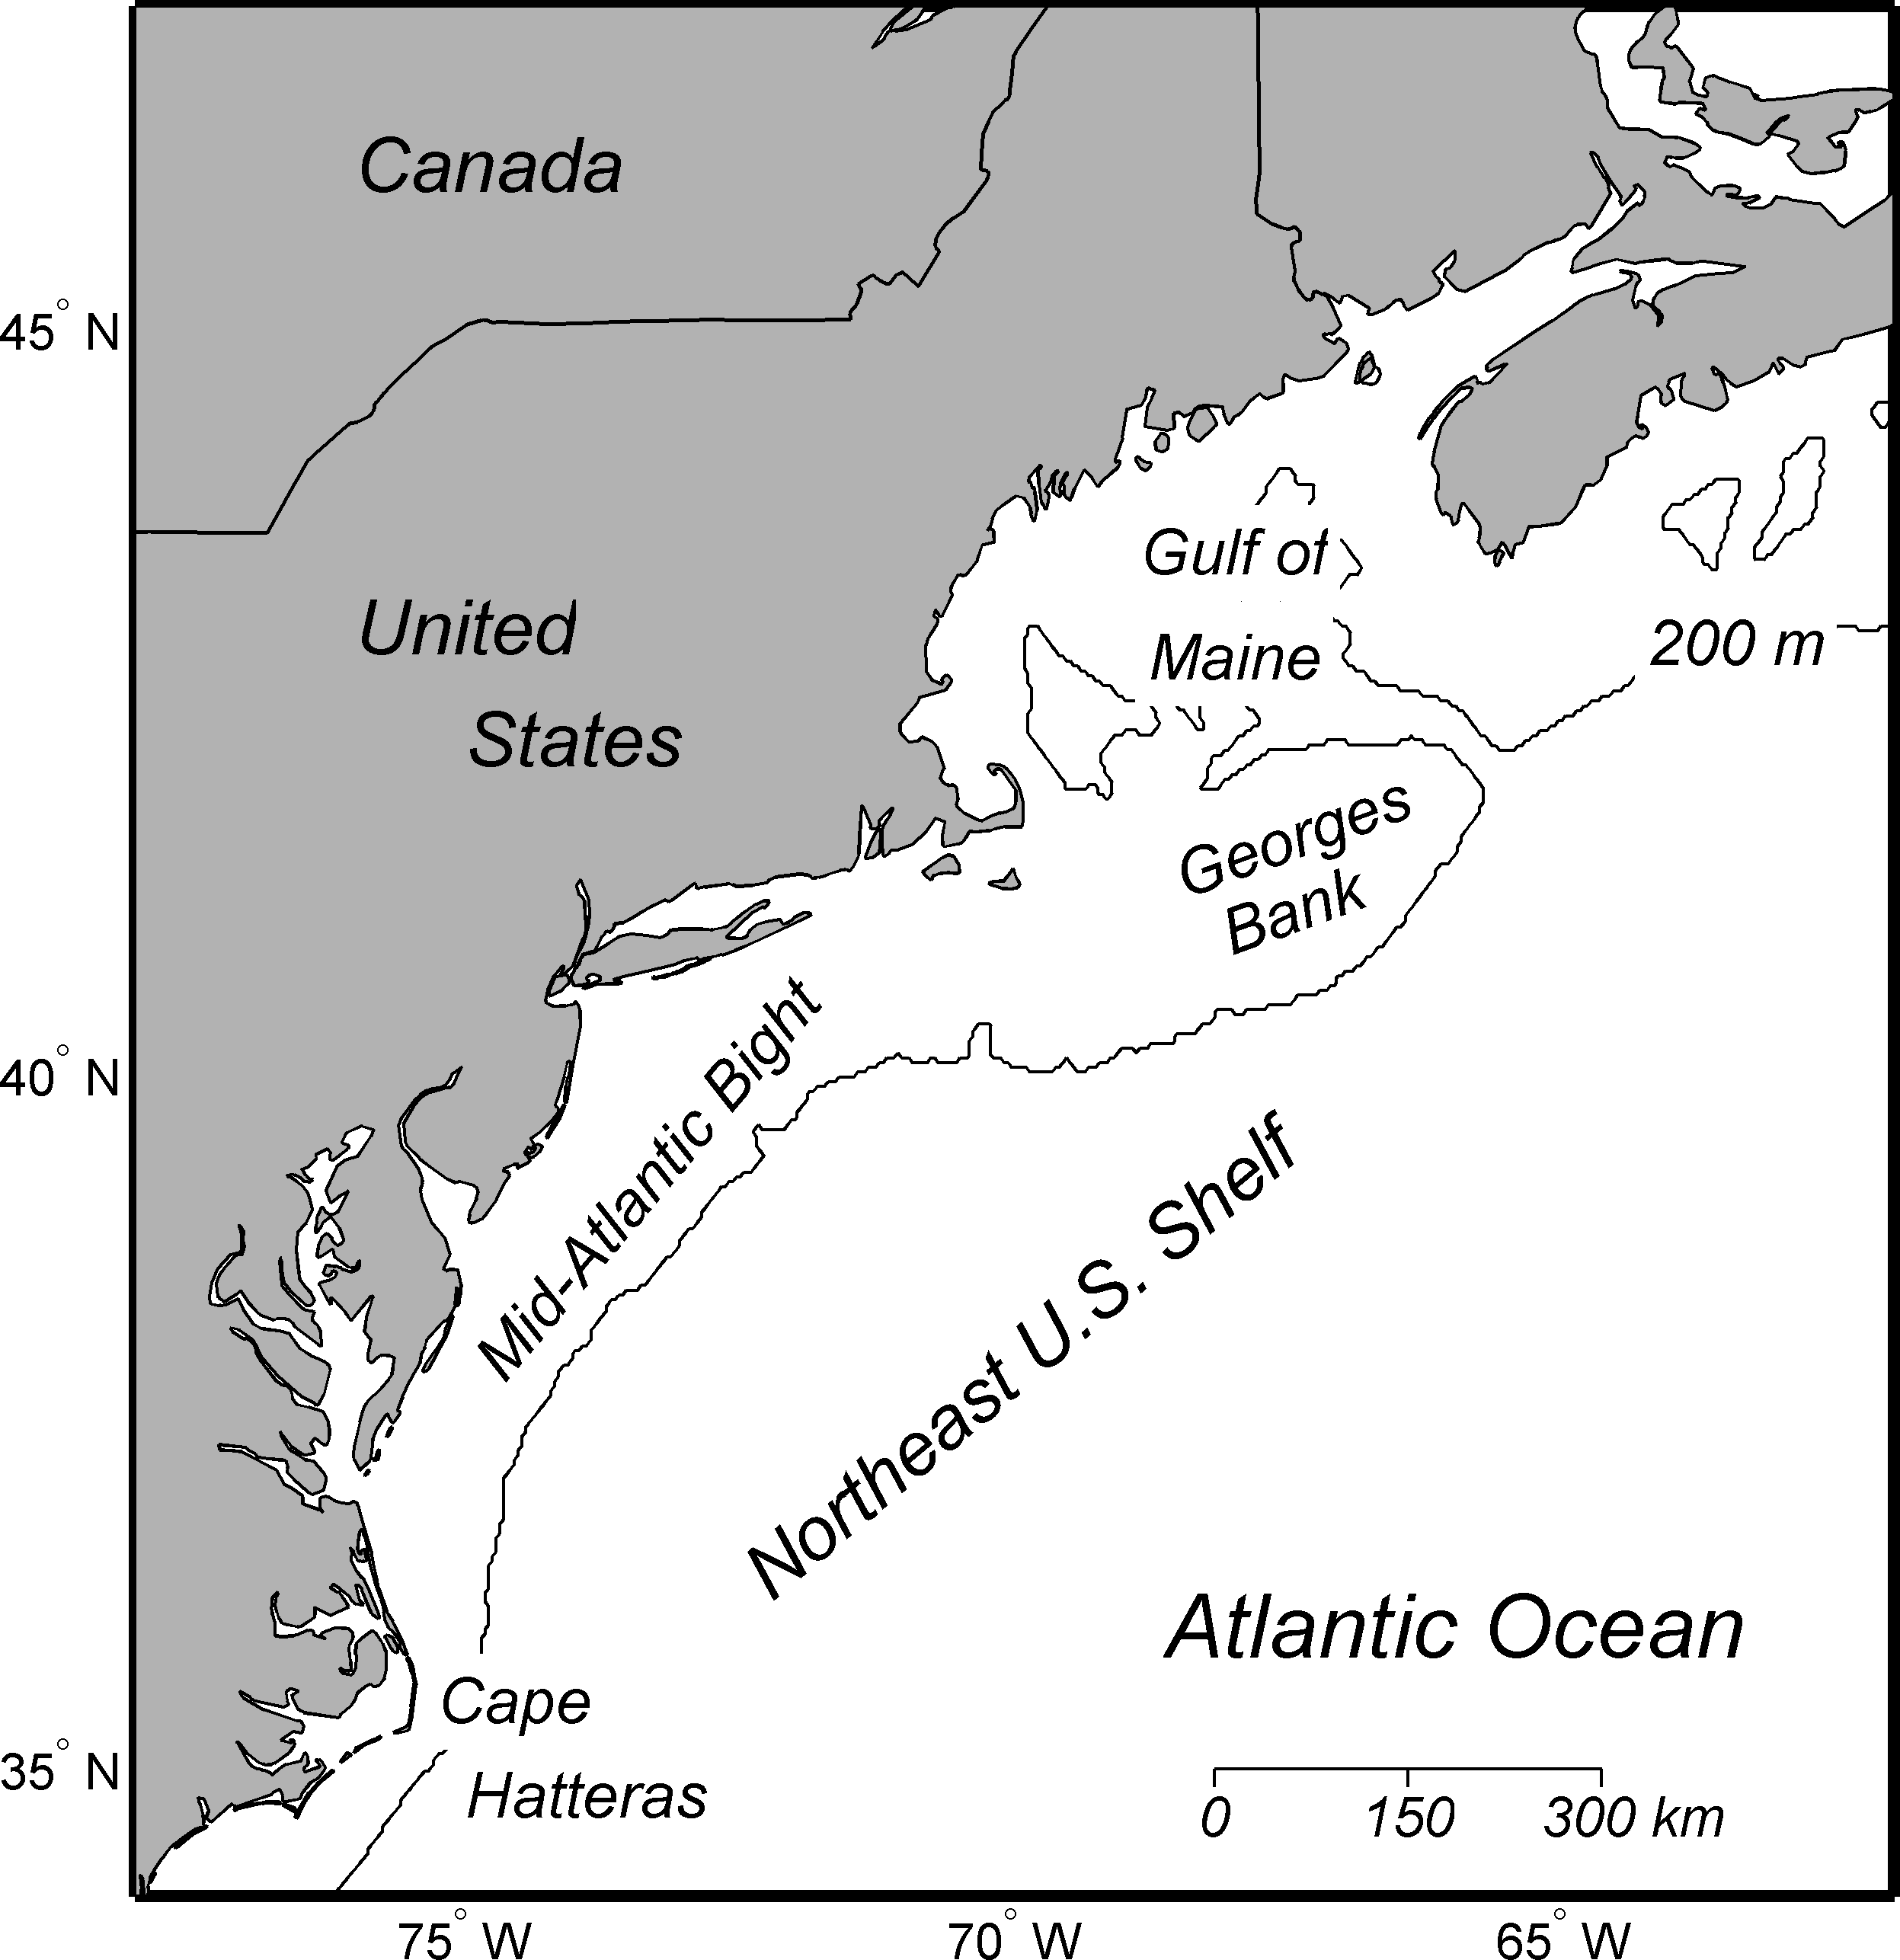
\includegraphics[width=34.64in]{images/journal.pone.0146756.g002} \end{center}

\chapter{Data and Code Access}\label{erddap}

\subsection{About}\label{about}

The Technical Documentation for the State of the Ecosystem (SOE) reports
is a \href{https://bookdown.org}{bookdown} document; hosted on the NOAA
Northeast Fisheries Science Center (NEFSC) Ecosystems Dynamics and
Assessment Branch \href{https://github.com/NOAA-EDAB}{Github page}, and
developed in R. Derived data used to populate figures in this document
are queried directly from the
\href{https://github.com/NOAA-EDAB/ecodata}{ecodata} R package or the
NEFSC
\href{https://comet.nefsc.noaa.gov/erddap/info/index.html?page=1\&itemsPerPage=1000}{ERDDAP
server}. ERDDAP queries are made using the R package
\href{https://cran.r-project.org/web/packages/rerddap/vignettes/Using_rerddap.html}{rerddap}.

\subsection{Accessing data and build
code}\label{accessing-data-and-build-code}

In this technical documentation, we hope to shine a light on the
processing and analytical steps involved to get from source data to
final product. This means that whenever possible, we have included the
code involved in source data extraction, processing, and analyses. We
have also attempted to thoroughly describe all methods in place of or in
supplement to provided code. Example plotting code for each indicator is
presented in sections titled ``Plotting'', and these code chunks can be
used to recreate the figures found in ecosystem reporting documents
where each respective indicator was included\footnote{There are multiple
  R scripts sourced throughout this document in an attempt to keep code
  concise. These scripts include
  \href{https://github.com/NOAA-EDAB/tech-doc/blob/master/R/BasePlot_source.R}{BasePlot\_source.R},
  \href{https://github.com/NOAA-EDAB/tech-doc/blob/master/R/GIS_source.R}{GIS\_source.R},
  and
  \href{https://github.com/NOAA-EDAB/tech-doc/blob/master/R/get_erddap.R}{get\_erddap.R}.
  The scripts \texttt{BasePlot\_source.R} and \texttt{GIS\_source.R}
  refer to deprecated code used prior to the 2019 State of the Ecosystem
  reports. Indicators that were not included in reports after 2018 make
  use of this syntax, whereas newer indicators typically use
  \texttt{ggplot2} for plotting.}.

Source data for the derived indicators in this document are linked to in
the text unless there are privacy concerns involved. In that case, it
may be possible to access source data by reaching out to the Point of
Contact associated with that data set. Derived data sets make up the
majority of the indicators presented in ecosystem reporting documents,
and these data sets are available for download through the
\href{https://github.com/NOAA-EDAB/ecodata}{ecodata} R package.

\subsection{Building the document}\label{building-the-document}

Start a local build of the SOE bookdown document by first cloning the
project's associated \href{https://github.com/NOAA-EDAB/tech-doc}{git
repository}. Next, if you would like to build a past version of the
document, use \texttt{git\ checkout\ {[}version\_commit\_hash{]}} to
revert the project to a past commit of interest, and set
\texttt{build\_latest\ \textless{}-\ FALSE} in the following code chunk.
This will ensure the project builds from a cached data set, and not the
most updated versions present on the NEFSC ERDDAP server. Once the
\texttt{tech-doc.Rproj} file is opened in RStudio, run
\texttt{bookdown::serve\_book()} from the console to build the document.

\begin{Shaded}
\begin{Highlighting}[]
\NormalTok{build_latest <-}\StringTok{ }\OtherTok{FALSE}

\ControlFlowTok{if}\NormalTok{ (build_latest)\{}
  
  \CommentTok{# Relative working directories}
\NormalTok{  data.dir  <-}\StringTok{ }\NormalTok{here}\OperatorTok{::}\KeywordTok{here}\NormalTok{(}\StringTok{'data'}\NormalTok{)}
\NormalTok{  r.dir <-}\StringTok{ }\NormalTok{here}\OperatorTok{::}\KeywordTok{here}\NormalTok{(}\StringTok{'R'}\NormalTok{)}
  
  \CommentTok{#Source function for querying ERDDAP server}
  \KeywordTok{source}\NormalTok{(}\KeywordTok{file.path}\NormalTok{(r.dir,}\StringTok{"get_erddap.R"}\NormalTok{))}
  
  \CommentTok{#Set URL for COMET (server where NEFSC ERDDAP lives)}
\NormalTok{  comet <-}\StringTok{ 'https://comet.nefsc.noaa.gov/erddap/'}
  
  \CommentTok{#List datasets on the NEFSC ERDDAP}
\NormalTok{  tab_list <-}\StringTok{ }\KeywordTok{ed_datasets}\NormalTok{(}\DataTypeTok{url =}\NormalTok{ comet)}
  
  \CommentTok{#Get updated data set IDs}
\NormalTok{  erddap_datasets <-}\StringTok{ }\NormalTok{tab_list }\OperatorTok\StringTok{ }
\StringTok{    }\KeywordTok{filter}\NormalTok{(}\KeywordTok{str_detect}\NormalTok{(Dataset.ID, }\StringTok{"soe_v"}\NormalTok{)) }\OperatorTok\StringTok{ }
\StringTok{    }\KeywordTok{get_erddap}\NormalTok{(}\DataTypeTok{id =} \OtherTok{NULL}\NormalTok{)}
  
  \CommentTok{#Save and clean updated IDs for use in rest of report}
  \KeywordTok{save}\NormalTok{(erddap_datasets, }\DataTypeTok{file =} \KeywordTok{file.path}\NormalTok{(data.dir, }\StringTok{"ERDDAP_datasets.Rdata"}\NormalTok{))}
  
  \CommentTok{# Exclude stock assessment status data, which have unique structure}
\NormalTok{  erddap_datasets <-}\StringTok{ }\NormalTok{erddap_datasets }\OperatorTok
\StringTok{    }\NormalTok{dplyr}\OperatorTok{::}\KeywordTok{filter}\NormalTok{(}\OperatorTok{!}\KeywordTok{str_detect}\NormalTok{(Dataset.ID, }\StringTok{"assess"}\NormalTok{)) }
  
  \CommentTok{#Create SOE parent data set, filter out NAs. This queries based on }
  \CommentTok{#data set IDs that were collected above}
\NormalTok{  SOE.data.erd <-}\StringTok{ }\KeywordTok{sprintf}\NormalTok{(}\StringTok{"http://comet.nefsc.noaa.gov/erddap/tabledap/%s.csv"}\NormalTok{,}
\NormalTok{                           erddap_datasets}\OperatorTok{$}\NormalTok{Dataset.ID) }\OperatorTok\StringTok{ }
\StringTok{    }\NormalTok{purrr}\OperatorTok{::}\KeywordTok{map}\NormalTok{(}\ControlFlowTok{function}\NormalTok{(x) \{}
\NormalTok{      readr}\OperatorTok{::}\KeywordTok{read_csv}\NormalTok{(}\KeywordTok{url}\NormalTok{(x))}
\NormalTok{    \}) }\OperatorTok\StringTok{ }
\StringTok{    }\KeywordTok{do.call}\NormalTok{(rbind,.) }\OperatorTok\StringTok{ }
\StringTok{    }\KeywordTok{mutate}\NormalTok{(}\DataTypeTok{Value =} \KeywordTok{as.numeric}\NormalTok{(Value)) }\OperatorTok\StringTok{ }
\StringTok{      }\NormalTok{dplyr}\OperatorTok{::}\KeywordTok{filter}\NormalTok{(}\OperatorTok{!}\KeywordTok{is.na}\NormalTok{(Value))}
  
  \CommentTok{#Convert to data.table}
\NormalTok{  SOE.data <-}\StringTok{ }\KeywordTok{as.data.table}\NormalTok{(SOE.data.erd)}
  
  \CommentTok{#Save data}
  \KeywordTok{save}\NormalTok{(SOE.data, }\DataTypeTok{file =} \KeywordTok{file.path}\NormalTok{(data.dir,}\StringTok{"SOE_data_erddap.Rdata"}\NormalTok{))}
\NormalTok{\}}
\end{Highlighting}
\end{Shaded}

\subsubsection{A note on data
structures}\label{a-note-on-data-structures}

The majority of the derived time series used in State of the Ecosystem
reports are in long format. This approach was taken so that all
disparate data sets could be ``bound'' together for ease of use in our
base plotting
\href{(https://github.com/NOAA-EDAB/tech-doc/blob/master/R/BasePlot_source.R)}{functions}.

\hypertarget{aggroups}{\chapter{Aggregate Groups}\label{aggroups}}

\textbf{Description}: Mappings of species into aggregate group
categories for different analyses

\textbf{Found in}: State of the Ecosystem - Gulf of Maine \& Georges
Bank (2018, 2019), State of the Ecosystem - Mid-Atlantic (2018, 2019)

\textbf{Indicator category}: Synthesis of published information

\textbf{Contributor(s)}: Geret DePiper, Sarah Gaichas, Sean Hardison,
Sean Lucey

\textbf{Data steward}: Sean Lucey
\href{mailto:Sean.Lucey@noaa.gov}{\nolinkurl{Sean.Lucey@noaa.gov}}

\textbf{Point of contact}: Sean Lucey
\href{mailto:Sean.Lucey@noaa.gov}{\nolinkurl{Sean.Lucey@noaa.gov}}

\textbf{Public availability statement}: Source data is available to the
public (see Data Sources).

\section{Methods}\label{methods}

The State of the Ecosystem (SOE) reports are delivered to the New
England Fishery Management Council (NEFMC) and Mid-Atlantic Fishery
Management Council (MAFMC) to provide ecosystems context. To better
understand that broader ecosystem context, many of the indicators are
reported at an aggregate level rather than at a single species level.
Species were assigned to an aggregate group following the classification
scheme of Garrison and Link
(\protect\hyperlink{ref-garrison2000dietary}{2000}) and Link et al.
(\protect\hyperlink{ref-link2006EMAX}{2006}). Both works classified
species into feeding guilds based on food habits data collected at the
Northeast Fisheries Science Center (NEFSC). In 2017, the SOE used seven
specific feeding guilds (plus an ``other'' category; Table
\ref{tab:soe2017class}). These seven were the same guilds used in
Garrison and Link (\protect\hyperlink{ref-garrison2000dietary}{2000}),
which also distinguished ontogentic shifts in species diets.

For the purposes of the SOE, species were only assigned to one category
based on the most prevalent size available to commercial fisheries.
However, several of those categories were confusing to the management
councils, so in 2018 those categories were simplified to five (plus
``other''; Table \ref{tab:soe2018class}) along the lines of Link et al.
(\protect\hyperlink{ref-link2006EMAX}{2006}). In addition to feeding
guilds, species managed by the councils have been identified. This is
done to show the breadth of what a given council is responsible for
within the broader ecosystem context.

\begin{table}

\caption{\label{tab:soe2017class}Aggregate groups use in 2017 SOE.  Classifications are based on @garrison2000dietary . \label{}}
\centering
\begin{tabular}[t]{ll}
\toprule
Feeding.Guild & Description\\
\midrule
Apex Predator & Top of the food chain\\
Piscivore & Fish eaters\\
Macrozoo-piscivore & Shrimp and small fish eaters\\
Macroplanktivore & Amphipod and shrimp eaters\\
Mesoplanktivore & Zooplankton eaters\\
\addlinespace
Benthivore & Bottom eaters\\
Benthos & Things that live on the bottom\\
Other & Things not classified above\\
\bottomrule
\end{tabular}
\end{table}

\begin{table}

\caption{\label{tab:soe2018class}Aggregate groups use in 2018 SOE.  Classifications are based on @link2006EMAX.}
\centering
\begin{tabular}[t]{ll}
\toprule
Feeding.Guild & Description\\
\midrule
Apex Predator & Top of the food chain\\
Piscivore & Fish eaters\\
Planktivore & Zooplankton eaters\\
Benthivore & Bottom eaters\\
Benthos & Things that live on the bottom\\
\addlinespace
Other & Things not classified above\\
\bottomrule
\end{tabular}
\end{table}

\subsection{Data sources}\label{data-sources}

In order to match aggregate groups with various data sources, a look-up
table was generated which includes species' common names (COMNAME) along
with their scientific names (SCINAME) and several species codes. SVSPP
codes are used by the NEFSC Ecosystems Surveys Branch (ESB) in their
fishery-independent Survey Database (SVDBS), while NESPP3 codes refer to
the codes used by the Commercial Fisheries Database System (CFDBS) for
fishery-dependent data. A third species code provided is the ITISSPP,
which refers to species identifiers used by the Integrated Taxonomic
Information System (ITIS). Digits within ITIS codes are hierarchical,
with different positions in the identifier referring to higher or lower
taxonomic levels. More information about the SVDBS, CFDBS, and ITIS
species codes are available in the links provided below.

Management responsibilities for different species are listed under the
column ``Fed.managed'' (NEFMC, MAFMC, or JOINT for jointly managed
species). More information about these species is available on the FMC
websites listed below. Species groupings listed in the ``NEIEA'' column
were developed for presentation on the Northeast Integrated Ecosystem
Assessment (NE-IEA) website. These groupings are based on EMAX groupings
(Link et al. \protect\hyperlink{ref-link2006EMAX}{2006}), but were
adjusted based on conceptual models developed for the NE-IEA program
that highlight focal components in the Northeast Large Marine Ecosystem
(i.e.~those components with the largest potential for perturbing
ecosystem dynamics). NE-IEA groupings were further simplified to allow
for effective communication through the NE-IEA website.

\subsubsection{Supplemental information}\label{supplemental-information}

See the following links for more information regarding the NEFSC ESB
Bottom Trawl Survey, CFDBS, and ITIS:

\begin{itemize}
\tightlist
\item
  \url{https://www.itis.gov/}\\
\item
  \url{https://inport.nmfs.noaa.gov/inport/item/22561}\\
\item
  \url{https://inport.nmfs.noaa.gov/inport/item/22560}\\
\item
  \url{https://inport.nmfs.noaa.gov/inport/item/27401}
\end{itemize}

More information about the NE-IEA program is available
\href{http://integratedecosystemassessment.noaa.gov}{here}.

More information about the New Engalnd Fisheries Management Council is
available \href{https://www.nefmc.org/}{here}.

More information about the Mid-Atlantic Fisheries Management Council is
available \href{http://www.mafmc.org/}{here}.

\subsection{Data extraction}\label{data-extraction}

Species lists are pulled from SVDBS and CFDBS. They are merged using the
ITIS code. Classifications from Garrison and Link (Garrison and Link
\protect\hyperlink{ref-garrison2000dietary}{2000}) and Link et al. (Link
et al. \protect\hyperlink{ref-link2006EMAX}{2006}) are added manually.
The R code used in the extraction process is presented below.

\begin{Shaded}
\begin{Highlighting}[]
\CommentTok{#Species list}
\ControlFlowTok{if}\NormalTok{(}\KeywordTok{Sys.info}\NormalTok{()[}\StringTok{'sysname'}\NormalTok{]}\OperatorTok{==}\StringTok{"Windows"}\NormalTok{)\{}
\NormalTok{  data.dir <-}\StringTok{ "L:}\CharTok{\textbackslash{}\textbackslash{}}\StringTok{EcoAP}\CharTok{\textbackslash{}\textbackslash{}}\StringTok{Data}\CharTok{\textbackslash{}\textbackslash{}}\StringTok{survey"}
\NormalTok{  out.dir  <-}\StringTok{ "L:}\CharTok{\textbackslash{}\textbackslash{}}\StringTok{EcoAP}\CharTok{\textbackslash{}\textbackslash{}}\StringTok{Data}\CharTok{\textbackslash{}\textbackslash{}}\StringTok{survey"}
  \KeywordTok{memory.limit}\NormalTok{(}\DecValTok{4000}\NormalTok{)}
\NormalTok{\}}
\ControlFlowTok{if}\NormalTok{(}\KeywordTok{Sys.info}\NormalTok{()[}\StringTok{'sysname'}\NormalTok{]}\OperatorTok{==}\StringTok{"Linux"}\NormalTok{)\{}
\NormalTok{  data.dir  <-}\StringTok{ "/home/slucey/slucey/EcoAP/Data/survey"}
\NormalTok{  out.dir   <-}\StringTok{ "/home/slucey/slucey/EcoAP/Data/survey"}
\NormalTok{  out.dir.}\DecValTok{2}\NormalTok{ <-}\StringTok{ "/home/slucey/slucey/EcoAP/Data/Commercial"}
\NormalTok{  uid       <-}\StringTok{ 'slucey'}
  \KeywordTok{cat}\NormalTok{(}\StringTok{"Oracle Password: "}\NormalTok{)}
\NormalTok{  pwd <-}\StringTok{ }\KeywordTok{scan}\NormalTok{(}\KeywordTok{stdin}\NormalTok{(), }\KeywordTok{character}\NormalTok{(), }\DataTypeTok{n =} \DecValTok{1}\NormalTok{)}
\NormalTok{\}}

\KeywordTok{library}\NormalTok{(RODBC); }\KeywordTok{library}\NormalTok{(data.table)}

\ControlFlowTok{if}\NormalTok{(}\KeywordTok{Sys.info}\NormalTok{()[}\StringTok{'sysname'}\NormalTok{]}\OperatorTok{==}\StringTok{"Windows"}\NormalTok{)\{}
\NormalTok{  channel <-}\StringTok{ }\KeywordTok{odbcDriverConnect}\NormalTok{()}
\NormalTok{\} }\ControlFlowTok{else}\NormalTok{ \{}
\NormalTok{  channel <-}\StringTok{ }\KeywordTok{odbcConnect}\NormalTok{(}\StringTok{'sole'}\NormalTok{, uid, pwd)}
\NormalTok{\}}

\CommentTok{#Grab svspp code by itis code}
\NormalTok{svspp <-}\StringTok{ }\KeywordTok{as.data.table}\NormalTok{(}\KeywordTok{sqlQuery}\NormalTok{(channel, }\StringTok{"select SVSPP, ITISSPP, COMNAME, SCINAME }
\StringTok{                                from ITIS_Lookup"}\NormalTok{))}

\CommentTok{#Grab cfspp by itis code}
\NormalTok{cfspp <-}\StringTok{ }\KeywordTok{as.data.table}\NormalTok{(}\KeywordTok{sqlQuery}\NormalTok{(channel, }\StringTok{"select NESPP4, SPECIES_ITIS, }
\StringTok{                                COMMON_NAME, SCIENTIFIC_NAME }
\StringTok{                                from CFDBS.Species_itis_ne"}\NormalTok{))}
\KeywordTok{setnames}\NormalTok{(cfspp, }\StringTok{'SPECIES_ITIS'}\NormalTok{, }\StringTok{'ITISSPP'}\NormalTok{)}
\NormalTok{cfspp[, NESPP3 }\OperatorTok{:}\ErrorTok{=}\StringTok{ }\KeywordTok{as.numeric}\NormalTok{(}\KeywordTok{substr}\NormalTok{(}\KeywordTok{sprintf}\NormalTok{(}\StringTok{'%04d'}\NormalTok{, NESPP4), }\DecValTok{1}\NormalTok{, }\DecValTok{3}\NormalTok{))]}
\KeywordTok{setkey}\NormalTok{(cfspp, NESPP3)}
\NormalTok{cfspp <-}\StringTok{ }\KeywordTok{unique}\NormalTok{(cfspp)}
\NormalTok{cfspp[, NESPP4 }\OperatorTok{:}\ErrorTok{=}\StringTok{ }\OtherTok{NULL}\NormalTok{]}

\KeywordTok{setkey}\NormalTok{(cfspp, ITISSPP, NESPP3)}
\NormalTok{cfspp <-}\StringTok{ }\KeywordTok{unique}\NormalTok{(cfspp, }\DataTypeTok{by =} \KeywordTok{key}\NormalTok{(cfspp))}

\CommentTok{#Merge to master species list}
\NormalTok{spp <-}\StringTok{ }\KeywordTok{merge}\NormalTok{(svspp, cfspp, }\DataTypeTok{by =} \StringTok{'ITISSPP'}\NormalTok{, }\DataTypeTok{all =}\NormalTok{ T)}
\NormalTok{spp <-}\StringTok{ }\NormalTok{spp[}\OperatorTok{!}\NormalTok{(}\KeywordTok{is.na}\NormalTok{(SVSPP) }\OperatorTok{&}\StringTok{ }\KeywordTok{is.na}\NormalTok{(NESPP3)), ]}

\CommentTok{#Fix known issues}
\NormalTok{spp <-}\StringTok{ }\NormalTok{spp[}\OperatorTok{!}\NormalTok{SVSPP }\OperatorTok\StringTok{ }\KeywordTok{c}\NormalTok{(}\DecValTok{193}\NormalTok{, }\DecValTok{310}\NormalTok{), ]}

\NormalTok{spp[ITISSPP }\OperatorTok{==}\StringTok{ }\DecValTok{630979}\NormalTok{, SVSPP  }\OperatorTok{:}\ErrorTok{=}\StringTok{ }\DecValTok{193}\NormalTok{] }\CommentTok{#Ocean Pout}
\NormalTok{spp[ITISSPP }\OperatorTok{==}\StringTok{ }\DecValTok{620992}\NormalTok{, SVSPP  }\OperatorTok{:}\ErrorTok{=}\StringTok{ }\DecValTok{310}\NormalTok{] }\CommentTok{#Deepsea red crab}
\NormalTok{spp[ITISSPP }\OperatorTok{==}\StringTok{ }\DecValTok{172783}\NormalTok{, SVSPP  }\OperatorTok{:}\ErrorTok{=}\StringTok{ }\DecValTok{104}\NormalTok{] }\CommentTok{#Fourspot flounder}
\NormalTok{spp[ITISSPP }\OperatorTok{==}\StringTok{ }\DecValTok{166283}\NormalTok{, SVSPP  }\OperatorTok{:}\ErrorTok{=}\StringTok{ }\DecValTok{112}\NormalTok{] }\CommentTok{#John Dory}
\NormalTok{spp[ITISSPP }\OperatorTok{==}\StringTok{ }\DecValTok{161731}\NormalTok{, SVSPP  }\OperatorTok{:}\ErrorTok{=}\StringTok{  }\DecValTok{36}\NormalTok{] }\CommentTok{#Menhaden}
\NormalTok{spp[ITISSPP }\OperatorTok{==}\StringTok{  }\DecValTok{98671}\NormalTok{, SVSPP  }\OperatorTok{:}\ErrorTok{=}\StringTok{ }\DecValTok{311}\NormalTok{] }\CommentTok{#Cancer Crabs unk}
\NormalTok{spp[ITISSPP }\OperatorTok{==}\StringTok{  }\DecValTok{98455}\NormalTok{, SVSPP  }\OperatorTok{:}\ErrorTok{=}\StringTok{ }\DecValTok{317}\NormalTok{] }\CommentTok{#Spider crabs}
\NormalTok{spp[ITISSPP }\OperatorTok{==}\StringTok{ }\DecValTok{159772}\NormalTok{, NESPP3 }\OperatorTok{:}\ErrorTok{=}\StringTok{ }\DecValTok{150}\NormalTok{] }\CommentTok{#Hagfish}
\NormalTok{spp[ITISSPP }\OperatorTok{==}\StringTok{ }\DecValTok{166284}\NormalTok{, NESPP3 }\OperatorTok{:}\ErrorTok{=}\StringTok{ }\DecValTok{188}\NormalTok{] }\CommentTok{#John Dory}
\NormalTok{spp[ITISSPP }\OperatorTok{==}\StringTok{ }\DecValTok{98670}\NormalTok{,  NESPP3 }\OperatorTok{:}\ErrorTok{=}\StringTok{ }\DecValTok{714}\NormalTok{] }\CommentTok{#Cancer Crabs unk}

\NormalTok{spp[ITISSPP }\OperatorTok\StringTok{ }\KeywordTok{c}\NormalTok{(}\DecValTok{630979}\NormalTok{, }\DecValTok{620992}\NormalTok{), COMNAME }\OperatorTok{:}\ErrorTok{=}\StringTok{ }\NormalTok{COMMON_NAME]}
\NormalTok{spp[ITISSPP }\OperatorTok\StringTok{ }\KeywordTok{c}\NormalTok{(}\DecValTok{630979}\NormalTok{, }\DecValTok{620992}\NormalTok{), SCINAME }\OperatorTok{:}\ErrorTok{=}\StringTok{ }\NormalTok{SCIENTIFIC_NAME]}

\CommentTok{#Drop extra columns}
\NormalTok{spp[}\KeywordTok{is.na}\NormalTok{(COMNAME), COMNAME }\OperatorTok{:}\ErrorTok{=}\StringTok{ }\NormalTok{COMMON_NAME]}
\NormalTok{spp[}\KeywordTok{is.na}\NormalTok{(SCINAME), SCINAME }\OperatorTok{:}\ErrorTok{=}\StringTok{ }\NormalTok{SCIENTIFIC_NAME]}
\NormalTok{spp[, }\KeywordTok{c}\NormalTok{(}\StringTok{'COMMON_NAME'}\NormalTok{, }\StringTok{'SCIENTIFIC_NAME'}\NormalTok{) }\OperatorTok{:}\ErrorTok{=}\StringTok{ }\OtherTok{NULL}\NormalTok{]}
\KeywordTok{setcolorder}\NormalTok{(spp, }\KeywordTok{c}\NormalTok{(}\StringTok{'ITISSPP'}\NormalTok{, }\StringTok{'SVSPP'}\NormalTok{, }\StringTok{'NESPP3'}\NormalTok{, }\StringTok{'COMNAME'}\NormalTok{, }\StringTok{'SCINAME'}\NormalTok{))}
\KeywordTok{setkey}\NormalTok{(spp, SVSPP, NESPP3)}

\CommentTok{#-------------------------------------------------------------------------------}
\CommentTok{#Add management authority}
\NormalTok{mafmc <-}\StringTok{ }\KeywordTok{c}\NormalTok{(}\DecValTok{103}\NormalTok{, }\DecValTok{121}\NormalTok{, }\DecValTok{131}\NormalTok{, }\DecValTok{135}\NormalTok{, }\DecValTok{141}\NormalTok{, }\DecValTok{143}\NormalTok{, }\DecValTok{151}\NormalTok{, }\DecValTok{403}\NormalTok{, }\DecValTok{409}\NormalTok{, }\DecValTok{502}\NormalTok{, }\DecValTok{503}\NormalTok{, }\DecValTok{621}\NormalTok{)}
\NormalTok{nefmc <-}\StringTok{ }\KeywordTok{c}\NormalTok{(}\DecValTok{22}\OperatorTok{:}\DecValTok{28}\NormalTok{, }\DecValTok{32}\NormalTok{, }\DecValTok{69}\NormalTok{, }\DecValTok{72}\OperatorTok{:}\DecValTok{77}\NormalTok{, }\DecValTok{101}\NormalTok{, }\DecValTok{102}\NormalTok{, }\DecValTok{105}\OperatorTok{:}\DecValTok{107}\NormalTok{, }\DecValTok{155}\NormalTok{, }\DecValTok{193}\NormalTok{, }\DecValTok{310}\NormalTok{, }\DecValTok{401}\NormalTok{, }\DecValTok{894}\NormalTok{)}
\NormalTok{joint <-}\StringTok{ }\KeywordTok{c}\NormalTok{(}\DecValTok{15}\NormalTok{, }\DecValTok{197}\NormalTok{)}
\NormalTok{spp[SVSPP }\OperatorTok\StringTok{ }\NormalTok{mafmc, MANAGE }\OperatorTok{:}\ErrorTok{=}\StringTok{ 'MAFMC'}\NormalTok{]}
\NormalTok{spp[SVSPP }\OperatorTok\StringTok{ }\NormalTok{nefmc, MANAGE }\OperatorTok{:}\ErrorTok{=}\StringTok{ 'NEFMC'}\NormalTok{]}
\NormalTok{spp[SVSPP }\OperatorTok\StringTok{ }\NormalTok{joint, MANAGE }\OperatorTok{:}\ErrorTok{=}\StringTok{ 'JOINT'}\NormalTok{]}

\CommentTok{#-------------------------------------------------------------------------------}
\CommentTok{#Add functional groups}
\CommentTok{#From NEFMC EBFM PDT work}
\CommentTok{#See Functional_group_table_Mike.csv in slucey/EcoAP/EBFM_PDT}
\NormalTok{spp[, EBFM.PDT }\OperatorTok{:}\ErrorTok{=}\StringTok{ }\KeywordTok{factor}\NormalTok{(}\OtherTok{NA}\NormalTok{, }\DataTypeTok{levels =} \KeywordTok{c}\NormalTok{(}\StringTok{'Apex Predator'}\NormalTok{, }\StringTok{'Benthivore'}\NormalTok{, }\StringTok{'Benthos'}\NormalTok{,}
                                        \StringTok{'Macroplanktivore'}\NormalTok{, }\StringTok{'Macrozoo-piscivore'}\NormalTok{,}
                                        \StringTok{'Mesoplanktivore'}\NormalTok{, }\StringTok{'Piscivore'}\NormalTok{, }\StringTok{'Other'}\NormalTok{))]}
\NormalTok{spp[SVSPP }\OperatorTok\StringTok{ }\KeywordTok{c}\NormalTok{(}\DecValTok{11}\NormalTok{, }\DecValTok{700}\NormalTok{, }\DecValTok{704}\NormalTok{, }\DecValTok{747}\NormalTok{), EBFM.PDT }\OperatorTok{:}\ErrorTok{=}\StringTok{ 'Apex Predator'}\NormalTok{]}
\NormalTok{spp[SVSPP }\OperatorTok\StringTok{ }\KeywordTok{c}\NormalTok{(}\DecValTok{14}\NormalTok{, }\DecValTok{22}\NormalTok{, }\DecValTok{25}\NormalTok{, }\DecValTok{74}\NormalTok{, }\DecValTok{102}\NormalTok{, }\DecValTok{105}\NormalTok{, }\DecValTok{106}\NormalTok{, }\DecValTok{107}\NormalTok{, }\DecValTok{141}\NormalTok{, }\DecValTok{143}\NormalTok{, }\DecValTok{151}\NormalTok{, }\DecValTok{164}\NormalTok{, }\DecValTok{172}\NormalTok{,}
                   \DecValTok{176}\NormalTok{, }\DecValTok{177}\NormalTok{, }\DecValTok{192}\NormalTok{, }\DecValTok{193}\NormalTok{, }\DecValTok{301}\NormalTok{, }\DecValTok{310}\NormalTok{, }\DecValTok{312}\NormalTok{, }\DecValTok{314}\NormalTok{, }\DecValTok{317}\NormalTok{, }\DecValTok{322}\NormalTok{, }\DecValTok{501}\NormalTok{),}
\NormalTok{    EBFM.PDT }\OperatorTok{:}\ErrorTok{=}\StringTok{ 'Benthivore'}\NormalTok{]}
\NormalTok{spp[SVSPP }\OperatorTok\StringTok{ }\KeywordTok{c}\NormalTok{(}\DecValTok{331}\NormalTok{, }\DecValTok{336}\NormalTok{, }\DecValTok{401}\NormalTok{, }\DecValTok{403}\NormalTok{, }\DecValTok{409}\NormalTok{), EBFM.PDT }\OperatorTok{:}\ErrorTok{=}\StringTok{ 'Benthos'}\NormalTok{]}
\NormalTok{spp[NESPP3 }\OperatorTok\StringTok{ }\KeywordTok{c}\NormalTok{(}\DecValTok{775}\NormalTok{, }\DecValTok{781}\NormalTok{, }\DecValTok{805}\NormalTok{, }\DecValTok{806}\NormalTok{), EBFM.PDT }\OperatorTok{:}\ErrorTok{=}\StringTok{ 'Benthos'}\NormalTok{]  }
\NormalTok{spp[SVSPP }\OperatorTok\StringTok{ }\KeywordTok{c}\NormalTok{(}\DecValTok{76}\NormalTok{, }\DecValTok{163}\NormalTok{, }\DecValTok{168}\NormalTok{, }\DecValTok{171}\NormalTok{, }\DecValTok{502}\NormalTok{, }\DecValTok{503}\NormalTok{), EBFM.PDT }\OperatorTok{:}\ErrorTok{=}\StringTok{ 'Macroplanktivore'}\NormalTok{]}
\NormalTok{spp[SVSPP }\OperatorTok\StringTok{ }\KeywordTok{c}\NormalTok{(}\DecValTok{13}\NormalTok{, }\DecValTok{24}\NormalTok{, }\DecValTok{26}\NormalTok{, }\DecValTok{27}\NormalTok{, }\DecValTok{75}\NormalTok{, }\DecValTok{77}\NormalTok{, }\DecValTok{84}\NormalTok{, }\DecValTok{108}\NormalTok{, }\DecValTok{112}\NormalTok{, }\DecValTok{155}\NormalTok{, }\DecValTok{156}\NormalTok{, }\DecValTok{311}\NormalTok{),}
\NormalTok{    EBFM.PDT }\OperatorTok{:}\ErrorTok{=}\StringTok{ 'Macrozoo-piscivore'}\NormalTok{]}
\NormalTok{spp[SVSPP }\OperatorTok\StringTok{ }\KeywordTok{c}\NormalTok{(}\DecValTok{32}\NormalTok{, }\DecValTok{33}\NormalTok{, }\DecValTok{34}\NormalTok{, }\DecValTok{35}\NormalTok{, }\DecValTok{36}\NormalTok{, }\DecValTok{121}\NormalTok{, }\DecValTok{131}\NormalTok{), EBFM.PDT }\OperatorTok{:}\ErrorTok{=}\StringTok{ 'Mesoplanktivore'}\NormalTok{]}
\NormalTok{spp[SVSPP }\OperatorTok\StringTok{ }\KeywordTok{c}\NormalTok{(}\DecValTok{15}\NormalTok{, }\DecValTok{23}\NormalTok{, }\DecValTok{28}\NormalTok{, }\DecValTok{69}\NormalTok{, }\DecValTok{72}\NormalTok{, }\DecValTok{73}\NormalTok{, }\DecValTok{101}\NormalTok{, }\DecValTok{103}\NormalTok{, }\DecValTok{104}\NormalTok{, }\DecValTok{135}\NormalTok{, }\DecValTok{139}\NormalTok{, }\DecValTok{145}\NormalTok{, }\DecValTok{197}\NormalTok{),}
\NormalTok{    EBFM.PDT }\OperatorTok{:}\ErrorTok{=}\StringTok{ 'Piscivore'}\NormalTok{]}
\NormalTok{spp[}\KeywordTok{is.na}\NormalTok{(EBFM.PDT), EBFM.PDT }\OperatorTok{:}\ErrorTok{=}\StringTok{ 'Other'}\NormalTok{]}

\CommentTok{#Fix known issues}
\NormalTok{spp[SVSPP }\OperatorTok{==}\StringTok{ }\DecValTok{160}\NormalTok{, EBFM.PDT }\OperatorTok{:}\ErrorTok{=}\StringTok{ 'Macroplanktivore'}\NormalTok{]}

\CommentTok{#Add EMAX}
\KeywordTok{load}\NormalTok{(}\KeywordTok{file.path}\NormalTok{(data.dir, }\StringTok{'EMAX_groups.RData'}\NormalTok{))}
\NormalTok{emax <-}\StringTok{ }\NormalTok{emax[}\OperatorTok{!}\KeywordTok{is.na}\NormalTok{(SVSPP), ]}
\NormalTok{spp <-}\StringTok{ }\KeywordTok{merge}\NormalTok{(spp, emax[, }\KeywordTok{list}\NormalTok{(SVSPP, EMAX, Fall.q, Spring.q)], }\DataTypeTok{by =} \StringTok{'SVSPP'}\NormalTok{, }\DataTypeTok{all.x =}\NormalTok{ T)}

\CommentTok{#reduce rows}
\KeywordTok{setkey}\NormalTok{(spp, SVSPP, NESPP3)}
\NormalTok{species <-}\StringTok{ }\KeywordTok{unique}\NormalTok{(spp, }\DataTypeTok{by =} \KeywordTok{key}\NormalTok{(spp))}

\CommentTok{#Remove EMAX q's}
\NormalTok{species[, }\KeywordTok{c}\NormalTok{(}\StringTok{'Fall.q'}\NormalTok{, }\StringTok{'Spring.q'}\NormalTok{) }\OperatorTok{:}\ErrorTok{=}\StringTok{ }\OtherTok{NULL}\NormalTok{]}

\CommentTok{#Expand EMAX abbreviations}
\NormalTok{species[EMAX }\OperatorTok{==}\StringTok{ 'BG'}\NormalTok{, EMAX }\OperatorTok{:}\ErrorTok{=}\StringTok{ 'Benthivore Gadiformes'}\NormalTok{]}
\NormalTok{species[EMAX }\OperatorTok{==}\StringTok{ 'BE'}\NormalTok{, EMAX }\OperatorTok{:}\ErrorTok{=}\StringTok{ 'Benthivore Elasmobranchs'}\NormalTok{]}
\NormalTok{species[EMAX }\OperatorTok{==}\StringTok{ 'BP'}\NormalTok{, EMAX }\OperatorTok{:}\ErrorTok{=}\StringTok{ 'Benthivore Pleuronectiformes'}\NormalTok{]}
\NormalTok{species[EMAX }\OperatorTok{==}\StringTok{ 'BS'}\NormalTok{, EMAX }\OperatorTok{:}\ErrorTok{=}\StringTok{ 'Benthivore Scorpaeniformes'}\NormalTok{]}
\NormalTok{species[EMAX }\OperatorTok{==}\StringTok{ 'BO'}\NormalTok{, EMAX }\OperatorTok{:}\ErrorTok{=}\StringTok{ 'Benthivore Others'}\NormalTok{]}
\NormalTok{species[EMAX }\OperatorTok{==}\StringTok{ 'BC'}\NormalTok{, EMAX }\OperatorTok{:}\ErrorTok{=}\StringTok{ 'Benthivore Perciformes'}\NormalTok{]}
\NormalTok{species[EMAX }\OperatorTok{==}\StringTok{ 'PG'}\NormalTok{, EMAX }\OperatorTok{:}\ErrorTok{=}\StringTok{ 'Piscivore Gadiformes'}\NormalTok{]}
\NormalTok{species[EMAX }\OperatorTok{==}\StringTok{ 'PE'}\NormalTok{, EMAX }\OperatorTok{:}\ErrorTok{=}\StringTok{ 'Piscivore Elasmobranchs'}\NormalTok{]}
\NormalTok{species[EMAX }\OperatorTok{==}\StringTok{ 'PO'}\NormalTok{, EMAX }\OperatorTok{:}\ErrorTok{=}\StringTok{ 'Piscivore Others'}\NormalTok{]}
\NormalTok{species[EMAX }\OperatorTok{==}\StringTok{ 'OE'}\NormalTok{, EMAX }\OperatorTok{:}\ErrorTok{=}\StringTok{ 'Omnivore Elasmobranchs'}\NormalTok{]}
\NormalTok{species[EMAX }\OperatorTok{==}\StringTok{ 'OO'}\NormalTok{, EMAX }\OperatorTok{:}\ErrorTok{=}\StringTok{ 'Omnivore Others'}\NormalTok{]}
\NormalTok{species[EMAX }\OperatorTok{==}\StringTok{ 'SC'}\NormalTok{, EMAX }\OperatorTok{:}\ErrorTok{=}\StringTok{ 'Southern Perciformes'}\NormalTok{]}
\NormalTok{species[EMAX }\OperatorTok{==}\StringTok{ 'SP'}\NormalTok{, EMAX }\OperatorTok{:}\ErrorTok{=}\StringTok{ 'Southern Pleuronectiformes'}\NormalTok{]}
\NormalTok{species[EMAX }\OperatorTok{==}\StringTok{ 'SE'}\NormalTok{, EMAX }\OperatorTok{:}\ErrorTok{=}\StringTok{ 'Southern Elasmobranchs'}\NormalTok{]}
\NormalTok{species[EMAX }\OperatorTok{==}\StringTok{ 'SG'}\NormalTok{, EMAX }\OperatorTok{:}\ErrorTok{=}\StringTok{ 'Southern Gadiformes'}\NormalTok{]}
\NormalTok{species[EMAX }\OperatorTok{==}\StringTok{ 'SO'}\NormalTok{, EMAX }\OperatorTok{:}\ErrorTok{=}\StringTok{ 'Southern Others'}\NormalTok{]}

\CommentTok{#Rename columns}
\KeywordTok{setnames}\NormalTok{(species, }\KeywordTok{c}\NormalTok{(}\StringTok{'MANAGE'}\NormalTok{, }\StringTok{'EBFM.PDT'}\NormalTok{, }\StringTok{'Feeding.guild'}\NormalTok{), }\KeywordTok{c}\NormalTok{(}\StringTok{'Fed.Managed'}\NormalTok{, }\StringTok{'SOE.17'}\NormalTok{, }\StringTok{'SOE.18'}\NormalTok{))}

\CommentTok{#Add classification from Garrison/Link 2000}
\NormalTok{size <-}\StringTok{ }\KeywordTok{data.table}\NormalTok{(}\DataTypeTok{COMNAME =} \KeywordTok{c}\NormalTok{(}\KeywordTok{rep}\NormalTok{(}\StringTok{'SMOOTH DOGFISH'}\NormalTok{,           }\DecValTok{2}\NormalTok{), }
                               \KeywordTok{rep}\NormalTok{(}\StringTok{'SPINY DOGFISH'}\NormalTok{,            }\DecValTok{3}\NormalTok{),}
                               \KeywordTok{rep}\NormalTok{(}\StringTok{'WINTER SKATE'}\NormalTok{,             }\DecValTok{4}\NormalTok{),}
                               \KeywordTok{rep}\NormalTok{(}\StringTok{'LITTLE SKATE'}\NormalTok{,             }\DecValTok{2}\NormalTok{),}
                               \KeywordTok{rep}\NormalTok{(}\StringTok{'SMOOTH SKATE'}\NormalTok{,             }\DecValTok{1}\NormalTok{),}
                               \KeywordTok{rep}\NormalTok{(}\StringTok{'THORNY SKATE'}\NormalTok{,             }\DecValTok{4}\NormalTok{),}
                               \KeywordTok{rep}\NormalTok{(}\StringTok{'ATLANTIC HERRING'}\NormalTok{,         }\DecValTok{2}\NormalTok{),}
                               \KeywordTok{rep}\NormalTok{(}\StringTok{'ALEWIFE'}\NormalTok{,                  }\DecValTok{1}\NormalTok{),}
                               \KeywordTok{rep}\NormalTok{(}\StringTok{'SILVER HAKE'}\NormalTok{,              }\DecValTok{3}\NormalTok{),}
                               \KeywordTok{rep}\NormalTok{(}\StringTok{'ATLANTIC COD'}\NormalTok{,             }\DecValTok{4}\NormalTok{),}
                               \KeywordTok{rep}\NormalTok{(}\StringTok{'HADDOCK'}\NormalTok{,                  }\DecValTok{3}\NormalTok{),}
                               \KeywordTok{rep}\NormalTok{(}\StringTok{'POLLOCK'}\NormalTok{,                  }\DecValTok{4}\NormalTok{),}
                               \KeywordTok{rep}\NormalTok{(}\StringTok{'WHITE HAKE'}\NormalTok{,               }\DecValTok{3}\NormalTok{),}
                               \KeywordTok{rep}\NormalTok{(}\StringTok{'RED HAKE'}\NormalTok{,                 }\DecValTok{3}\NormalTok{),}
                               \KeywordTok{rep}\NormalTok{(}\StringTok{'SPOTTED HAKE'}\NormalTok{,             }\DecValTok{2}\NormalTok{),}
                               \KeywordTok{rep}\NormalTok{(}\StringTok{'AMERICAN PLAICE'}\NormalTok{,          }\DecValTok{3}\NormalTok{), }
                               \KeywordTok{rep}\NormalTok{(}\StringTok{'SUMMER FLOUNDER'}\NormalTok{,          }\DecValTok{2}\NormalTok{),}
                               \KeywordTok{rep}\NormalTok{(}\StringTok{'FOURSPOT FLOUNDER'}\NormalTok{,        }\DecValTok{2}\NormalTok{),}
                               \KeywordTok{rep}\NormalTok{(}\StringTok{'YELLOWTAIL FLOUNDER'}\NormalTok{,      }\DecValTok{3}\NormalTok{),}
                               \KeywordTok{rep}\NormalTok{(}\StringTok{'WINTER FLOUNDER'}\NormalTok{,          }\DecValTok{3}\NormalTok{),}
                               \KeywordTok{rep}\NormalTok{(}\StringTok{'WITCH FLOUNDER'}\NormalTok{,           }\DecValTok{2}\NormalTok{), }
                               \KeywordTok{rep}\NormalTok{(}\StringTok{'WINDOWPANE'}\NormalTok{,               }\DecValTok{2}\NormalTok{),}
                               \KeywordTok{rep}\NormalTok{(}\StringTok{'GULF STREAM FLOUNDER'}\NormalTok{,     }\DecValTok{1}\NormalTok{), }
                               \KeywordTok{rep}\NormalTok{(}\StringTok{'ATLANTIC MACKEREL'}\NormalTok{,        }\DecValTok{3}\NormalTok{),}
                               \KeywordTok{rep}\NormalTok{(}\StringTok{'BUTTERFISH'}\NormalTok{,               }\DecValTok{1}\NormalTok{),}
                               \KeywordTok{rep}\NormalTok{(}\StringTok{'BLUEFISH'}\NormalTok{,                 }\DecValTok{3}\NormalTok{),}
                               \KeywordTok{rep}\NormalTok{(}\StringTok{'ATLANTIC CROAKER'}\NormalTok{,         }\DecValTok{2}\NormalTok{),}
                               \KeywordTok{rep}\NormalTok{(}\StringTok{'BLACK SEA BASS'}\NormalTok{,           }\DecValTok{2}\NormalTok{), }
                               \KeywordTok{rep}\NormalTok{(}\StringTok{'SCUP'}\NormalTok{,                     }\DecValTok{1}\NormalTok{),}
                               \KeywordTok{rep}\NormalTok{(}\StringTok{'WEAKFISH'}\NormalTok{,                 }\DecValTok{2}\NormalTok{),}
                               \KeywordTok{rep}\NormalTok{(}\StringTok{'ACADIAN REDFISH'}\NormalTok{,          }\DecValTok{1}\NormalTok{),}
                               \KeywordTok{rep}\NormalTok{(}\StringTok{'LONGHORN SCULPIN'}\NormalTok{,         }\DecValTok{2}\NormalTok{),}
                               \KeywordTok{rep}\NormalTok{(}\StringTok{'SEA RAVEN'}\NormalTok{,                }\DecValTok{2}\NormalTok{),}
                               \KeywordTok{rep}\NormalTok{(}\StringTok{'NORTHERN SAND LANCE'}\NormalTok{,      }\DecValTok{1}\NormalTok{),}
                               \KeywordTok{rep}\NormalTok{(}\StringTok{'OCEAN POUT'}\NormalTok{,               }\DecValTok{1}\NormalTok{),}
                               \KeywordTok{rep}\NormalTok{(}\StringTok{'FAWN CUSK-EEL'}\NormalTok{,            }\DecValTok{1}\NormalTok{),}
                               \KeywordTok{rep}\NormalTok{(}\StringTok{'GOOSEFISH'}\NormalTok{,                }\DecValTok{1}\NormalTok{),}
                               \KeywordTok{rep}\NormalTok{(}\StringTok{'ATLANTIC SHARPNOSE SHARK'}\NormalTok{, }\DecValTok{1}\NormalTok{), }
                               \KeywordTok{rep}\NormalTok{(}\StringTok{'NORTHERN SHORTFIN SQUID'}\NormalTok{,  }\DecValTok{1}\NormalTok{),}
                               \KeywordTok{rep}\NormalTok{(}\StringTok{'LONGFIN SQUID'}\NormalTok{,            }\DecValTok{1}\NormalTok{)),}
                   \DataTypeTok{SizeCat =} \KeywordTok{c}\NormalTok{(}\StringTok{'M'}\NormalTok{, }\StringTok{'L'}\NormalTok{, }\StringTok{'S'}\NormalTok{, }\StringTok{'M'}\NormalTok{, }\StringTok{'L'}\NormalTok{, }\StringTok{'S'}\NormalTok{, }\StringTok{'M'}\NormalTok{, }\StringTok{'L'}\NormalTok{, }\StringTok{'XL'}\NormalTok{, }\StringTok{'S'}\NormalTok{,}
                               \StringTok{'M'}\NormalTok{, }\StringTok{'M'}\NormalTok{, }\StringTok{'S'}\NormalTok{, }\StringTok{'M'}\NormalTok{, }\StringTok{'L'}\NormalTok{, }\StringTok{'XL'}\NormalTok{, }\StringTok{'S'}\NormalTok{,}\StringTok{'M'}\NormalTok{,}\StringTok{'M'}\NormalTok{, }\StringTok{'S'}\NormalTok{,}
                               \StringTok{'M'}\NormalTok{, }\StringTok{'L'}\NormalTok{, }\StringTok{'S'}\NormalTok{, }\StringTok{'M'}\NormalTok{, }\StringTok{'L'}\NormalTok{, }\StringTok{'XL'}\NormalTok{, }\StringTok{'S'}\NormalTok{, }\StringTok{'M'}\NormalTok{, }\StringTok{'L'}\NormalTok{, }\StringTok{'S'}\NormalTok{,}
                               \StringTok{'M'}\NormalTok{, }\StringTok{'L'}\NormalTok{, }\StringTok{'XL'}\NormalTok{, }\StringTok{'S'}\NormalTok{, }\StringTok{'M'}\NormalTok{, }\StringTok{'L'}\NormalTok{, }\StringTok{'S'}\NormalTok{, }\StringTok{'M'}\NormalTok{, }\StringTok{'L'}\NormalTok{, }\StringTok{'S'}\NormalTok{,}
                               \StringTok{'M'}\NormalTok{,  }\StringTok{'S'}\NormalTok{, }\StringTok{'M'}\NormalTok{, }\StringTok{'L'}\NormalTok{, }\StringTok{'M'}\NormalTok{, }\StringTok{'L'}\NormalTok{, }\StringTok{'S'}\NormalTok{, }\StringTok{'M'}\NormalTok{, }\StringTok{'S'}\NormalTok{, }\StringTok{'M'}\NormalTok{,}
                               \StringTok{'L'}\NormalTok{, }\StringTok{'S'}\NormalTok{, }\StringTok{'M'}\NormalTok{, }\StringTok{'L'}\NormalTok{, }\StringTok{'M'}\NormalTok{, }\StringTok{'L'}\NormalTok{, }\StringTok{'S'}\NormalTok{, }\StringTok{'M'}\NormalTok{, }\StringTok{'S'}\NormalTok{, }\StringTok{'S'}\NormalTok{,}
                               \StringTok{'M'}\NormalTok{, }\StringTok{'L'}\NormalTok{, }\StringTok{'S'}\NormalTok{, }\StringTok{'S'}\NormalTok{, }\StringTok{'M'}\NormalTok{, }\StringTok{'L'}\NormalTok{, }\StringTok{'S'}\NormalTok{, }\StringTok{'M'}\NormalTok{, }\StringTok{'S'}\NormalTok{, }\StringTok{'M'}\NormalTok{,}
                               \StringTok{'M'}\NormalTok{, }\StringTok{'S'}\NormalTok{, }\StringTok{'M'}\NormalTok{, }\StringTok{'M'}\NormalTok{, }\StringTok{'S'}\NormalTok{, }\StringTok{'M'}\NormalTok{, }\StringTok{'S'}\NormalTok{, }\StringTok{'M'}\NormalTok{, }\StringTok{'M'}\NormalTok{, }\StringTok{'L'}\NormalTok{,}
                               \StringTok{'L'}\NormalTok{, }\StringTok{'L'}\NormalTok{, }\StringTok{'L'}\NormalTok{, }\StringTok{'L'}\NormalTok{, }\StringTok{'L'}\NormalTok{),}
                   \DataTypeTok{Min.size =} \KeywordTok{c}\NormalTok{(}\DecValTok{41}\NormalTok{, }\DecValTok{61}\NormalTok{, }\DecValTok{10}\NormalTok{, }\DecValTok{41}\NormalTok{, }\DecValTok{61}\NormalTok{, }\DecValTok{10}\NormalTok{, }\DecValTok{31}\NormalTok{, }\DecValTok{61}\NormalTok{, }\DecValTok{81}\NormalTok{, }\DecValTok{10}\NormalTok{, }\DecValTok{31}\NormalTok{, }\DecValTok{31}\NormalTok{,}
                                \DecValTok{10}\NormalTok{, }\DecValTok{31}\NormalTok{, }\DecValTok{61}\NormalTok{, }\DecValTok{81}\NormalTok{, }\DecValTok{10}\NormalTok{, }\DecValTok{21}\NormalTok{, }\DecValTok{21}\NormalTok{, }\DecValTok{10}\NormalTok{, }\DecValTok{21}\NormalTok{, }\DecValTok{41}\NormalTok{, }\DecValTok{10}\NormalTok{, }\DecValTok{21}\NormalTok{, }
                                \DecValTok{51}\NormalTok{, }\DecValTok{81}\NormalTok{, }\DecValTok{10}\NormalTok{, }\DecValTok{21}\NormalTok{, }\DecValTok{51}\NormalTok{, }\DecValTok{10}\NormalTok{, }\DecValTok{21}\NormalTok{, }\DecValTok{51}\NormalTok{, }\DecValTok{81}\NormalTok{, }\DecValTok{10}\NormalTok{, }\DecValTok{21}\NormalTok{, }\DecValTok{41}\NormalTok{, }\DecValTok{10}\NormalTok{, }\DecValTok{21}\NormalTok{, }\DecValTok{41}\NormalTok{, }\DecValTok{10}\NormalTok{, }\DecValTok{21}\NormalTok{, }
                                \DecValTok{10}\NormalTok{, }\DecValTok{21}\NormalTok{, }\DecValTok{41}\NormalTok{, }\DecValTok{21}\NormalTok{, }\DecValTok{41}\NormalTok{, }\DecValTok{10}\NormalTok{, }\DecValTok{21}\NormalTok{, }\DecValTok{10}\NormalTok{, }\DecValTok{21}\NormalTok{, }\DecValTok{41}\NormalTok{, }\DecValTok{10}\NormalTok{, }\DecValTok{21}\NormalTok{, }
                                \DecValTok{41}\NormalTok{, }\DecValTok{21}\NormalTok{, }\DecValTok{41}\NormalTok{, }\DecValTok{10}\NormalTok{, }\DecValTok{21}\NormalTok{, }\DecValTok{10}\NormalTok{, }\DecValTok{10}\NormalTok{, }\DecValTok{21}\NormalTok{, }\DecValTok{36}\NormalTok{, }\DecValTok{10}\NormalTok{, }\DecValTok{10}\NormalTok{, }\DecValTok{31}\NormalTok{,}
                                \DecValTok{71}\NormalTok{, }\DecValTok{10}\NormalTok{, }\DecValTok{26}\NormalTok{, }\DecValTok{10}\NormalTok{, }\DecValTok{26}\NormalTok{, }\DecValTok{26}\NormalTok{, }\DecValTok{10}\NormalTok{, }\DecValTok{26}\NormalTok{, }\DecValTok{26}\NormalTok{, }\DecValTok{10}\NormalTok{, }\DecValTok{26}\NormalTok{, }\DecValTok{10}\NormalTok{, }
                                \DecValTok{26}\NormalTok{, }\DecValTok{11}\NormalTok{, }\DecValTok{61}\NormalTok{, }\DecValTok{61}\NormalTok{, }\DecValTok{61}\NormalTok{, }\DecValTok{61}\NormalTok{, }\DecValTok{31}\NormalTok{, }\DecValTok{31}\NormalTok{),}
                   \DataTypeTok{Garrison.Link =} \KeywordTok{as.character}\NormalTok{(}\KeywordTok{c}\NormalTok{(}\DecValTok{1}\NormalTok{, }\DecValTok{1}\NormalTok{, }\DecValTok{2}\NormalTok{, }\DecValTok{2}\NormalTok{, }\DecValTok{6}\NormalTok{, }\DecValTok{3}\NormalTok{, }\DecValTok{3}\NormalTok{, }\DecValTok{6}\NormalTok{, }\DecValTok{6}\NormalTok{, }\DecValTok{3}\NormalTok{, }\DecValTok{3}\NormalTok{, }\DecValTok{4}\NormalTok{, }\DecValTok{5}\NormalTok{, }\DecValTok{5}\NormalTok{, }\DecValTok{6}\NormalTok{, }
                                     \DecValTok{6}\NormalTok{, }\DecValTok{2}\NormalTok{, }\DecValTok{2}\NormalTok{, }\DecValTok{2}\NormalTok{, }\DecValTok{4}\NormalTok{, }\DecValTok{4}\NormalTok{, }\DecValTok{6}\NormalTok{, }\DecValTok{3}\NormalTok{, }\DecValTok{3}\NormalTok{, }\DecValTok{6}\NormalTok{, }\DecValTok{6}\NormalTok{, }\DecValTok{5}\NormalTok{, }\DecValTok{5}\NormalTok{, }\DecValTok{5}\NormalTok{, }\DecValTok{4}\NormalTok{, }
                                     \DecValTok{4}\NormalTok{, }\DecValTok{4}\NormalTok{, }\DecValTok{4}\NormalTok{, }\DecValTok{3}\NormalTok{, }\DecValTok{4}\NormalTok{, }\DecValTok{6}\NormalTok{, }\DecValTok{3}\NormalTok{, }\DecValTok{3}\NormalTok{, }\DecValTok{4}\NormalTok{, }\DecValTok{3}\NormalTok{, }\DecValTok{6}\NormalTok{, }\DecValTok{5}\NormalTok{, }\DecValTok{5}\NormalTok{, }\DecValTok{5}\NormalTok{, }\DecValTok{6}\NormalTok{,}
                                     \DecValTok{6}\NormalTok{, }\DecValTok{3}\NormalTok{, }\DecValTok{6}\NormalTok{, }\DecValTok{3}\NormalTok{, }\DecValTok{5}\NormalTok{, }\DecValTok{5}\NormalTok{, }\DecValTok{5}\NormalTok{, }\DecValTok{5}\NormalTok{, }\DecValTok{5}\NormalTok{, }\DecValTok{5}\NormalTok{, }\DecValTok{5}\NormalTok{, }\DecValTok{3}\NormalTok{, }\DecValTok{3}\NormalTok{, }\DecValTok{5}\NormalTok{, }\DecValTok{2}\NormalTok{,}
                                     \DecValTok{2}\NormalTok{, }\DecValTok{2}\NormalTok{, }\DecValTok{2}\NormalTok{, }\DecValTok{6}\NormalTok{, }\DecValTok{6}\NormalTok{, }\DecValTok{6}\NormalTok{, }\DecValTok{5}\NormalTok{, }\DecValTok{5}\NormalTok{, }\DecValTok{1}\NormalTok{, }\DecValTok{1}\NormalTok{, }\DecValTok{5}\NormalTok{, }\DecValTok{6}\NormalTok{, }\DecValTok{6}\NormalTok{, }\DecValTok{4}\NormalTok{, }\DecValTok{3}\NormalTok{, }
                                     \DecValTok{3}\NormalTok{, }\DecValTok{6}\NormalTok{, }\DecValTok{6}\NormalTok{, }\DecValTok{2}\NormalTok{, }\DecValTok{5}\NormalTok{, }\DecValTok{3}\NormalTok{, }\DecValTok{6}\NormalTok{, }\DecValTok{6}\NormalTok{, }\DecValTok{2}\NormalTok{, }\DecValTok{2}\NormalTok{))}
\NormalTok{                                )}

\CommentTok{#Give Garrison.link guilds meaniful names}
\NormalTok{size[Garrison.Link }\OperatorTok{==}\StringTok{ }\DecValTok{1}\NormalTok{, Garrison.Link }\OperatorTok{:}\ErrorTok{=}\StringTok{ 'Crab Eaters'}\NormalTok{]}
\NormalTok{size[Garrison.Link }\OperatorTok{==}\StringTok{ }\DecValTok{2}\NormalTok{, Garrison.Link }\OperatorTok{:}\ErrorTok{=}\StringTok{ 'Planktivores'}\NormalTok{]}
\NormalTok{size[Garrison.Link }\OperatorTok{==}\StringTok{ }\DecValTok{3}\NormalTok{, Garrison.Link }\OperatorTok{:}\ErrorTok{=}\StringTok{ 'Amphipod/Shrimp Eaters'}\NormalTok{]}
\NormalTok{size[Garrison.Link }\OperatorTok{==}\StringTok{ }\DecValTok{4}\NormalTok{, Garrison.Link }\OperatorTok{:}\ErrorTok{=}\StringTok{ 'Shrimp/Small Fish Eaters'}\NormalTok{]}
\NormalTok{size[Garrison.Link }\OperatorTok{==}\StringTok{ }\DecValTok{5}\NormalTok{, Garrison.Link }\OperatorTok{:}\ErrorTok{=}\StringTok{ 'Benthivores'}\NormalTok{]}
\NormalTok{size[Garrison.Link }\OperatorTok{==}\StringTok{ }\DecValTok{6}\NormalTok{, Garrison.Link }\OperatorTok{:}\ErrorTok{=}\StringTok{ 'Piscivores'}\NormalTok{]}

\CommentTok{#Merge Garrison Link into species list}
\NormalTok{species <-}\StringTok{ }\KeywordTok{merge}\NormalTok{(species, size, }\DataTypeTok{by =} \StringTok{'COMNAME'}\NormalTok{, }\DataTypeTok{all =}\NormalTok{ T)}

\CommentTok{#Set column order}
\KeywordTok{setcolorder}\NormalTok{(species, }\KeywordTok{c}\NormalTok{(}\StringTok{'ITISSPP'}\NormalTok{, }\StringTok{'SVSPP'}\NormalTok{, }\StringTok{'NESPP3'}\NormalTok{, }\StringTok{'COMNAME'}\NormalTok{, }\StringTok{'SCINAME'}\NormalTok{, }
                       \StringTok{'SizeCat'}\NormalTok{, }\StringTok{'Min.size'}\NormalTok{, }\StringTok{'Fed.Managed'}\NormalTok{, }\StringTok{'Garrison.Link'}\NormalTok{,}
                       \StringTok{'SOE.17'}\NormalTok{, }\StringTok{'SOE.18'}\NormalTok{, }\StringTok{'EMAX'}\NormalTok{))}

\CommentTok{#Add NE.IEA.web category}
\CommentTok{#get rerddap}
\NormalTok{devtools}\OperatorTok{::}\KeywordTok{install_github}\NormalTok{(}\StringTok{"ropensci/rerddap"}\NormalTok{)}
\KeywordTok{library}\NormalTok{(rerddap) }

\CommentTok{#Set URL for COMET (server where NEFSC ERDDAP lives)}
\NormalTok{comet <-}\StringTok{ 'https://comet.nefsc.noaa.gov/erddap/'}

\CommentTok{#List datasets on the NEFSC ERDDAP}
\NormalTok{tab_list <-}\StringTok{ }\KeywordTok{ed_datasets}\NormalTok{(}\DataTypeTok{url =}\NormalTok{ comet)}

\CommentTok{#download a tabular dataset (input is dataset id; this works on vectors)}
\NormalTok{ed_spp <-}\StringTok{ }\KeywordTok{as.data.table}\NormalTok{(}\KeywordTok{sprintf}\NormalTok{(}\StringTok{"https://comet.nefsc.noaa.gov/erddap/tabledap/%s.csv"}\NormalTok{, }\StringTok{"species_groups_2018"}\NormalTok{) }\OperatorTok\StringTok{ }
\StringTok{  }
\StringTok{  }\NormalTok{purrr}\OperatorTok{::}\KeywordTok{map}\NormalTok{(}\ControlFlowTok{function}\NormalTok{(x) \{}
    
\NormalTok{    readr}\OperatorTok{::}\KeywordTok{read_csv}\NormalTok{(}\KeywordTok{url}\NormalTok{(x))}
    
\NormalTok{  \}))}

\NormalTok{neiea <-}\StringTok{ }\KeywordTok{unique}\NormalTok{(ed_spp[}\OperatorTok{!}\KeywordTok{is.na}\NormalTok{(NEIEA), }\KeywordTok{list}\NormalTok{(COMNAME, NEIEA)])}

\NormalTok{species <-}\StringTok{ }\KeywordTok{merge}\NormalTok{(species, neiea, }\DataTypeTok{by =} \StringTok{'COMNAME'}\NormalTok{, }\DataTypeTok{all =}\NormalTok{ T)}

\KeywordTok{save}\NormalTok{(species, }\DataTypeTok{file =} \KeywordTok{file.path}\NormalTok{(out.dir, }\StringTok{'SOE_species_list.RData'}\NormalTok{))}
\end{Highlighting}
\end{Shaded}

\chapter{Annual SST Cycles}\label{annual-sst-cycles}

\textbf{Description}: Annual SST Cycles

\textbf{Found in}: State of the Ecosystem - Gulf of Maine \& Georges
Bank (2018), State of the Ecosystem - Mid-Atlantic (2018)

\textbf{Indicator category}: Database pull with analysis

\textbf{Contributor(s)}: Sean Hardison, Vincent Saba

\textbf{Data steward}: Sean Hardison,
\href{mailto:sean.hardison@noaa.gov}{\nolinkurl{sean.hardison@noaa.gov}}

\textbf{Point of contact}: Sean Hardison,
\href{mailto:sean.hardison@noaa.gov}{\nolinkurl{sean.hardison@noaa.gov}}

\textbf{Public availability statement}: Source data are available
\href{https://www.esrl.noaa.gov/psd/data/gridded/data.noaa.oisst.v2.highres.html}{here}.

\section{Methods}\label{methods-1}

\subsection{Data sources}\label{data-sources-1}

Data for annual sea surface tempature (SST) cycles were derived from the
NOAA optimum interpolation sea surface temperature (OISST) high
resolution dataset
(\href{https://www.esrl.noaa.gov/psd/data/gridded/data.noaa.oisst.v2.highres.html}{NOAA
OISST V2 dataset}) provided by NOAA's Earth System Research Laboratory's
Physical Sciences Devision, Boulder, CO. The data extend from 1981 to
present, and provide a 0.25° x 0.25° global grid of SST measurements
(Reynolds et al. \protect\hyperlink{ref-Reynolds2007}{2007}). Gridded
SST data were masked according to the extent of Ecological Production
Units (EPU) in the Northeast Large Marine Ecosystem (NE-LME) (See
\href{https://github.com/NOAA-EDAB/tech-doc/tree/master/gis}{``EPU\_Extended''
shapefiles}).

\subsection{Data extraction}\label{data-extraction-1}

Daily mean sea surface temperature data for 2017 and for each year
during the period of 1981-2012 were downloaded from the NOAA
\href{https://www.esrl.noaa.gov/psd/data/gridded/data.noaa.oisst.v2.highres.html}{OI
SST V2 site} to derive the long-term climatological mean for the period.
The use of a 30-year climatological reference period is a standard
procedure for metereological observing (WMO
\protect\hyperlink{ref-WMO2017}{2017}). These reference periods serve as
benchmarks for comparing current or recent observations, and for the
development of standard anomaly data sets. The reference period of
1982-2012 was chosen to be consistent with previous versions of the
State of the Ecosystem report.

R code used in extraction and processing:

\begin{Shaded}
\begin{Highlighting}[]
\CommentTok{#libraries}
\KeywordTok{library}\NormalTok{(ncdf4);}\KeywordTok{library}\NormalTok{(dplyr)}
\KeywordTok{library}\NormalTok{(readr);}\KeywordTok{library}\NormalTok{(tidyr)}
\KeywordTok{library}\NormalTok{(sp);}\KeywordTok{library}\NormalTok{(rgdal)}
\KeywordTok{library}\NormalTok{(raster);}\KeywordTok{library}\NormalTok{(stringr)}

\CommentTok{#get spatial polygons for Ecological Production Units (EPUs) that are used to clip SST data.}
\NormalTok{EPU <-}\StringTok{ }\KeywordTok{readOGR}\NormalTok{(}\StringTok{'Extended_EPU'}\NormalTok{)}

\NormalTok{map.crs <-}\StringTok{ }\KeywordTok{CRS}\NormalTok{(}\StringTok{"+proj=longlat +lat_1=35 +lat_2=45 +lat_0=40 +lon_0=-77 +x_0=0}
\StringTok{               +y_0=0 +datum=NAD83 +no_defs +ellps=GRS80 +towgs84=0,0,0"}\NormalTok{)}

\CommentTok{#find long term daily mean SSTs and 2017 SST anomaly}
\NormalTok{MAB_sst_daily_mean <-}\StringTok{ }\OtherTok{NULL}
\NormalTok{GB_sst_daily_mean <-}\StringTok{ }\OtherTok{NULL}
\NormalTok{GOM_sst_daily_mean <-}\StringTok{ }\OtherTok{NULL}

\CommentTok{#I split the data into three directories to loop through in separate R sessions concurrently. }


\ControlFlowTok{for}\NormalTok{ (dir. }\ControlFlowTok{in} \DecValTok{1}\OperatorTok{:}\DecValTok{3}\NormalTok{)\{}
  
  \CommentTok{#Loop through directories}
  \KeywordTok{setwd}\NormalTok{(}\KeywordTok{paste0}\NormalTok{(}\StringTok{'c:/users/sean.hardison/documents/sst_data/'}\NormalTok{,dir.))}
  \KeywordTok{print}\NormalTok{(}\KeywordTok{getwd}\NormalTok{())}
  
  \ControlFlowTok{for}\NormalTok{ (f }\ControlFlowTok{in} \DecValTok{1}\OperatorTok{:}\KeywordTok{length}\NormalTok{(}\KeywordTok{list.files}\NormalTok{()))\{}
    
    \ControlFlowTok{if}\NormalTok{ (}\OperatorTok{!}\KeywordTok{str_detect}\NormalTok{(}\KeywordTok{list.files}\NormalTok{()[f],}\StringTok{".nc"}\NormalTok{))\{}
      \KeywordTok{print}\NormalTok{(}\KeywordTok{paste}\NormalTok{(}\KeywordTok{list.files}\NormalTok{()[f],}\StringTok{"is not a raster"}\NormalTok{)) }\CommentTok{#Based on file type}
      \ControlFlowTok{next}
\NormalTok{    \}}
    
    \ControlFlowTok{for}\NormalTok{ (j }\ControlFlowTok{in} \KeywordTok{c}\NormalTok{(}\StringTok{"MAB"}\NormalTok{,}\StringTok{"GB"}\NormalTok{,}\StringTok{"GOM"}\NormalTok{))\{}
      
\NormalTok{      sub_region <-}\StringTok{ }\NormalTok{EPU[EPU}\OperatorTok{@}\NormalTok{data}\OperatorTok{$}\NormalTok{EPU }\OperatorTok{==}\StringTok{ }\NormalTok{j,]}
\NormalTok{      y <-}\StringTok{ }\KeywordTok{as.numeric}\NormalTok{(}\KeywordTok{str_extract}\NormalTok{(}\KeywordTok{list.files}\NormalTok{()[f],}\StringTok{"[0-9]+"}\NormalTok{)) }\CommentTok{#get year}
      
      \ControlFlowTok{for}\NormalTok{ (i }\ControlFlowTok{in} \DecValTok{1}\OperatorTok{:}\DecValTok{365}\NormalTok{)\{}
        \KeywordTok{print}\NormalTok{(}\KeywordTok{paste}\NormalTok{(j,y,i))}
\NormalTok{        daily_mean <-}\StringTok{ }\KeywordTok{raster}\NormalTok{(}\KeywordTok{paste0}\NormalTok{(}\KeywordTok{list.files}\NormalTok{()[f]), }\DataTypeTok{band =}\NormalTok{ i) }\CommentTok{#get band}
        
        \CommentTok{#set crs}
\NormalTok{        daily_mean}\OperatorTok{@}\NormalTok{crs <-}\StringTok{ }\NormalTok{sub_region}\OperatorTok{@}\NormalTok{proj4string }
        
        
        \CommentTok{#rotate to lon scale from 0-360 to -180-180}
\NormalTok{        daily_mean <-}\StringTok{ }\KeywordTok{rotate}\NormalTok{(daily_mean)}
        
        \CommentTok{#mask raster with spatialpolygon}
\NormalTok{        daily_mean_clipped <-}\StringTok{ }\KeywordTok{mask}\NormalTok{(daily_mean, sub_region)}
        
        
        \CommentTok{#add mean value to data.frame}
        \KeywordTok{assign}\NormalTok{(}\KeywordTok{paste0}\NormalTok{(j,}\StringTok{"_sst_daily_mean"}\NormalTok{),}\KeywordTok{rbind}\NormalTok{(}\KeywordTok{get}\NormalTok{(}\KeywordTok{paste0}\NormalTok{(j,}\StringTok{"_sst_daily_mean"}\NormalTok{)),}
                                                 \KeywordTok{c}\NormalTok{(}\KeywordTok{mean}\NormalTok{(daily_mean_clipped}\OperatorTok{@}\NormalTok{data}\OperatorTok{@}\NormalTok{values, }\DataTypeTok{na.rm =}\NormalTok{ T),y,i)))}
        
\NormalTok{      \}}
\NormalTok{    \}}
    
    
\NormalTok{  \}}
\NormalTok{\}}

\CommentTok{#Put results into data.frames}
\NormalTok{mab <-}\StringTok{ }\KeywordTok{data.frame}\NormalTok{(}\DataTypeTok{EPU =} \StringTok{"MAB"}\NormalTok{,}
                  \DataTypeTok{year =}\NormalTok{ MAB_sst_daily_mean[,}\DecValTok{2}\NormalTok{],}
                  \DataTypeTok{day =}\NormalTok{ MAB_sst_daily_mean[,}\DecValTok{3}\NormalTok{],}
                  \DataTypeTok{Value =}\NormalTok{ MAB_sst_daily_mean[,}\DecValTok{1}\NormalTok{])}

\NormalTok{gb <-}\StringTok{ }\KeywordTok{data.frame}\NormalTok{(}\DataTypeTok{EPU =} \StringTok{"GB"}\NormalTok{,}
                 \DataTypeTok{year =}\NormalTok{ GB_sst_daily_mean[,}\DecValTok{2}\NormalTok{],}
                 \DataTypeTok{day =}\NormalTok{ GB_sst_daily_mean[,}\DecValTok{3}\NormalTok{],}
                 \DataTypeTok{Value =}\NormalTok{ GB_sst_daily_mean[,}\DecValTok{1}\NormalTok{])}

\NormalTok{gom <-}\StringTok{ }\KeywordTok{data.frame}\NormalTok{(}\DataTypeTok{EPU =} \StringTok{"GOM"}\NormalTok{,}
                  \DataTypeTok{year =}\NormalTok{ GOM_sst_daily_mean[,}\DecValTok{2}\NormalTok{],}
                  \DataTypeTok{day =}\NormalTok{ GOM_sst_daily_mean[,}\DecValTok{3}\NormalTok{],}
                  \DataTypeTok{Value =}\NormalTok{ GOM_sst_daily_mean[,}\DecValTok{1}\NormalTok{])}


\NormalTok{data3 <-}\StringTok{ }\KeywordTok{rbind}\NormalTok{(mab, gb, gom)}

\CommentTok{#Save as 1 of 3 files (one for each directory containing daily mean data)}
\KeywordTok{save}\NormalTok{(data3, }\DataTypeTok{file =} \StringTok{"dir3_sst.Rdata"}\NormalTok{)}

\CommentTok{#--------------------------2017 SSTs----------------------------#}
\NormalTok{MAB_}\DecValTok{2017}\NormalTok{ <-}\StringTok{ }\OtherTok{NULL}
\NormalTok{GB_}\DecValTok{2017}\NormalTok{ <-}\StringTok{ }\OtherTok{NULL}
\NormalTok{GOM_}\DecValTok{2017}\NormalTok{ <-}\StringTok{ }\OtherTok{NULL}

\ControlFlowTok{for}\NormalTok{ (j }\ControlFlowTok{in} \KeywordTok{c}\NormalTok{(}\StringTok{"MAB"}\NormalTok{,}\StringTok{"GB"}\NormalTok{,}\StringTok{"GOM"}\NormalTok{))\{}
  
\NormalTok{  sub_region <-}\StringTok{ }\NormalTok{EPU[EPU}\OperatorTok{@}\NormalTok{data}\OperatorTok{$}\NormalTok{EPU }\OperatorTok{==}\StringTok{ }\NormalTok{j,]}
  
  \ControlFlowTok{for}\NormalTok{ (i }\ControlFlowTok{in} \DecValTok{1}\OperatorTok{:}\DecValTok{365}\NormalTok{)\{}
    \KeywordTok{print}\NormalTok{(}\KeywordTok{paste}\NormalTok{(j,i))}
\NormalTok{    daily_mean <-}\StringTok{ }\KeywordTok{raster}\NormalTok{(}\StringTok{"sst.day.mean.2017.nc"}\NormalTok{, }\DataTypeTok{band =}\NormalTok{ i) }\CommentTok{#get band}
    
    
    \CommentTok{#set crs}
\NormalTok{    daily_mean}\OperatorTok{@}\NormalTok{crs <-}\StringTok{ }\NormalTok{sub_region}\OperatorTok{@}\NormalTok{proj4string }
    
    
    \CommentTok{#rotate to lon scale from 0-360 to -180-180}
\NormalTok{    daily_mean <-}\StringTok{ }\KeywordTok{rotate}\NormalTok{(daily_mean)}
    
    \CommentTok{#mask raster with spatialpolygon}
\NormalTok{    daily_mean_clipped <-}\StringTok{ }\KeywordTok{mask}\NormalTok{(daily_mean, sub_region)}
    
    
    \CommentTok{#add mean value to data.frame}
    \KeywordTok{assign}\NormalTok{(}\KeywordTok{paste0}\NormalTok{(j,}\StringTok{"_2017"}\NormalTok{),}\KeywordTok{rbind}\NormalTok{(}\KeywordTok{get}\NormalTok{(}\KeywordTok{paste0}\NormalTok{(j,}\StringTok{"_2017"}\NormalTok{)),}
                                             \KeywordTok{c}\NormalTok{(}\KeywordTok{mean}\NormalTok{(daily_mean_clipped}\OperatorTok{@}\NormalTok{data}\OperatorTok{@}\NormalTok{values, }\DataTypeTok{na.rm =}\NormalTok{ T),}\StringTok{"2017"}\NormalTok{,i)))}
    
\NormalTok{  \}}
\NormalTok{\}}
\CommentTok{#Put results into data.frames}
\NormalTok{mab_}\DecValTok{2017}\NormalTok{ <-}\StringTok{ }\KeywordTok{data.frame}\NormalTok{(}\DataTypeTok{EPU =} \StringTok{"MAB"}\NormalTok{,}
                  \DataTypeTok{year =}\NormalTok{ MAB_}\DecValTok{2017}\NormalTok{[,}\DecValTok{2}\NormalTok{],}
                  \DataTypeTok{day =}\NormalTok{ MAB_}\DecValTok{2017}\NormalTok{[,}\DecValTok{3}\NormalTok{],}
                  \DataTypeTok{Value =}\NormalTok{ MAB_}\DecValTok{2017}\NormalTok{[,}\DecValTok{1}\NormalTok{])}

\NormalTok{gb_}\DecValTok{2017}\NormalTok{ <-}\StringTok{ }\KeywordTok{data.frame}\NormalTok{(}\DataTypeTok{EPU =} \StringTok{"GB"}\NormalTok{,}
                 \DataTypeTok{year =}\NormalTok{ GB_}\DecValTok{2017}\NormalTok{[,}\DecValTok{2}\NormalTok{],}
                 \DataTypeTok{day =}\NormalTok{ GB_}\DecValTok{2017}\NormalTok{[,}\DecValTok{3}\NormalTok{],}
                 \DataTypeTok{Value =}\NormalTok{ GB_}\DecValTok{2017}\NormalTok{[,}\DecValTok{1}\NormalTok{])}

\NormalTok{gom_}\DecValTok{2017}\NormalTok{ <-}\StringTok{ }\KeywordTok{data.frame}\NormalTok{(}\DataTypeTok{EPU =} \StringTok{"GOM"}\NormalTok{,}
                  \DataTypeTok{year =}\NormalTok{ GOM_}\DecValTok{2017}\NormalTok{[,}\DecValTok{2}\NormalTok{],}
                  \DataTypeTok{day =}\NormalTok{ GOM_}\DecValTok{2017}\NormalTok{[,}\DecValTok{3}\NormalTok{],}
                  \DataTypeTok{Value =}\NormalTok{ GOM_}\DecValTok{2017}\NormalTok{[,}\DecValTok{1}\NormalTok{])}


\CommentTok{#Final 2017 daily mean data}
\NormalTok{sst_}\DecValTok{2017}\NormalTok{ <-}\StringTok{ }\KeywordTok{rbind}\NormalTok{(mab_}\DecValTok{2017}\NormalTok{, gb_}\DecValTok{2017}\NormalTok{, gom_}\DecValTok{2017}\NormalTok{)}
\CommentTok{#save(sst_2017, file = "sst_2017.Rdata")}
\end{Highlighting}
\end{Shaded}

\subsection{Data analysis}\label{data-analysis}

We calculated the long-term mean and standard deviation of SST over the
period of 1982-2012 for each EPU, as well as the daily mean for 2017.

\begin{Shaded}
\begin{Highlighting}[]
\CommentTok{#----------------------Load results--------------------------#}
\KeywordTok{load}\NormalTok{(}\StringTok{"dir1_sst.Rdata"}\NormalTok{)}
\KeywordTok{load}\NormalTok{(}\StringTok{"dir2_sst.Rdata"}\NormalTok{)}
\KeywordTok{load}\NormalTok{(}\StringTok{"dir3_sst.Rdata"}\NormalTok{)}
\KeywordTok{load}\NormalTok{(}\StringTok{"sst_2017.Rdata"}\NormalTok{)}

\CommentTok{#Get long term mean and standard deviation}
\NormalTok{d <-}\StringTok{ }\KeywordTok{rbind}\NormalTok{(data1, data2, data3)}

\NormalTok{ltm <-}\StringTok{ }\NormalTok{d }\OperatorTok\StringTok{ }\KeywordTok{group_by}\NormalTok{(EPU, day) }\OperatorTok\StringTok{ }\NormalTok{dplyr}\OperatorTok{::}\KeywordTok{summarise}\NormalTok{(}\DataTypeTok{mean  =} \KeywordTok{mean}\NormalTok{(Value),}
                                                     \DataTypeTok{sd =} \KeywordTok{sd}\NormalTok{(Value)) }
\end{Highlighting}
\end{Shaded}

\subsection{Plotting}\label{plotting}

\begin{Shaded}
\begin{Highlighting}[]
\CommentTok{# Relative working directories}
\NormalTok{data.dir  <-}\StringTok{ }\NormalTok{here}\OperatorTok{::}\KeywordTok{here}\NormalTok{(}\StringTok{'data'}\NormalTok{)}
\NormalTok{r.dir <-}\StringTok{ }\NormalTok{here}\OperatorTok{::}\KeywordTok{here}\NormalTok{(}\StringTok{'R'}\NormalTok{)}

\CommentTok{# Load data}
\KeywordTok{load}\NormalTok{(}\KeywordTok{file.path}\NormalTok{(data.dir,}\StringTok{"SOE_data_erddap.Rdata"}\NormalTok{))}

\NormalTok{##---------------------------------MAB-----------------------------------------#}
\KeywordTok{par}\NormalTok{(}\DataTypeTok{mfrow =} \KeywordTok{c}\NormalTok{(}\DecValTok{1}\NormalTok{,}\DecValTok{3}\NormalTok{))}
\NormalTok{doy <-}\StringTok{ }\KeywordTok{as.numeric}\NormalTok{(SOE.data[SOE.data}\OperatorTok{$}\NormalTok{Var }\OperatorTok{==}\StringTok{ "sst mean 2017 MAB"}\NormalTok{,]}\OperatorTok{$}\NormalTok{Time)}
\NormalTok{val_}\DecValTok{2017}\NormalTok{ <-}\StringTok{ }\NormalTok{SOE.data[SOE.data}\OperatorTok{$}\NormalTok{Var }\OperatorTok{==}\StringTok{ "sst mean 2017 MAB"}\NormalTok{,]}\OperatorTok{$}\NormalTok{Value}
\NormalTok{val_LT <-}\StringTok{ }\NormalTok{SOE.data[SOE.data}\OperatorTok{$}\NormalTok{Var }\OperatorTok{==}\StringTok{ "sst mean long term MAB"}\NormalTok{,]}\OperatorTok{$}\NormalTok{Value}
\NormalTok{val_LT_sd <-}\StringTok{ }\NormalTok{SOE.data[SOE.data}\OperatorTok{$}\NormalTok{Var }\OperatorTok{==}\StringTok{ "sst sd long term MAB"}\NormalTok{,]}\OperatorTok{$}\NormalTok{Value}


\CommentTok{# val_2017 <- approx(doy,val_2017, xout = seq(doy[1],doy[length(doy)],length.out = 365*1))$y}
\CommentTok{# val_LT <- approx(doy,val_LT, xout = seq(doy[1],doy[length(doy)],length.out = 365*1))$y}
\CommentTok{# val_LT_sd <- approx(doy,val_LT_sd, xout = seq(doy[1],doy[length(doy)],length.out = 365*1))$y}
\NormalTok{doy <-}\StringTok{ }\KeywordTok{seq}\NormalTok{(doy[}\DecValTok{1}\NormalTok{],doy[}\KeywordTok{length}\NormalTok{(doy)],}\DataTypeTok{length.out =} \DecValTok{365}\OperatorTok{*}\DecValTok{1}\NormalTok{)}


\NormalTok{above_mean <-}\StringTok{ }\OtherTok{NULL}
\ControlFlowTok{for}\NormalTok{ (i }\ControlFlowTok{in} \DecValTok{1}\OperatorTok{:}\KeywordTok{length}\NormalTok{(val_}\DecValTok{2017}\NormalTok{))\{}
  \ControlFlowTok{if}\NormalTok{ (val_}\DecValTok{2017}\NormalTok{[i] }\OperatorTok{>=}\StringTok{ }\NormalTok{val_LT[i])\{}
\NormalTok{    above_mean[i] <-}\StringTok{ }\NormalTok{val_}\DecValTok{2017}\NormalTok{[i]}
\NormalTok{  \} }\ControlFlowTok{else} \ControlFlowTok{if}\NormalTok{ (val_}\DecValTok{2017}\NormalTok{[i] }\OperatorTok{<}\StringTok{ }\NormalTok{val_LT [i])\{}
\NormalTok{    above_mean[i] <-}\StringTok{ }\OtherTok{NA}
\NormalTok{  \}}
\NormalTok{\}}

\NormalTok{below_mean <-}\StringTok{ }\OtherTok{NULL}
\ControlFlowTok{for}\NormalTok{ (i }\ControlFlowTok{in} \DecValTok{1}\OperatorTok{:}\KeywordTok{length}\NormalTok{(val_}\DecValTok{2017}\NormalTok{))\{}
  \ControlFlowTok{if}\NormalTok{ (val_}\DecValTok{2017}\NormalTok{[i] }\OperatorTok{<=}\StringTok{ }\NormalTok{val_LT[i])\{}
\NormalTok{    below_mean[i] <-}\StringTok{ }\NormalTok{val_}\DecValTok{2017}\NormalTok{[i]}
\NormalTok{  \} }\ControlFlowTok{else} \ControlFlowTok{if}\NormalTok{ (val_}\DecValTok{2017}\NormalTok{[i] }\OperatorTok{>}\StringTok{ }\NormalTok{val_LT [i])\{}
\NormalTok{    below_mean[i] <-}\StringTok{ }\OtherTok{NA}
\NormalTok{  \}}
\NormalTok{\}}

\NormalTok{above_sd <-}\StringTok{ }\OtherTok{NULL}
\ControlFlowTok{for}\NormalTok{ (i }\ControlFlowTok{in} \DecValTok{1}\OperatorTok{:}\KeywordTok{length}\NormalTok{(val_}\DecValTok{2017}\NormalTok{))\{}
  \ControlFlowTok{if}\NormalTok{ (val_}\DecValTok{2017}\NormalTok{[i] }\OperatorTok{>=}\StringTok{ }\NormalTok{val_LT_sd[i] }\OperatorTok{+}\StringTok{ }\NormalTok{val_LT[i])\{}
\NormalTok{    above_sd[i] <-}\StringTok{ }\NormalTok{val_}\DecValTok{2017}\NormalTok{[i]}
\NormalTok{  \} }\ControlFlowTok{else} \ControlFlowTok{if}\NormalTok{ (val_}\DecValTok{2017}\NormalTok{[i] }\OperatorTok{<}\StringTok{ }\NormalTok{val_LT_sd [i] }\OperatorTok{+}\StringTok{ }\NormalTok{val_LT[i])\{}
\NormalTok{    above_sd[i] <-}\StringTok{ }\OtherTok{NA}
\NormalTok{  \}}
\NormalTok{\}}

\NormalTok{below_sd <-}\StringTok{ }\OtherTok{NULL}
\ControlFlowTok{for}\NormalTok{ (i }\ControlFlowTok{in} \DecValTok{1}\OperatorTok{:}\KeywordTok{length}\NormalTok{(val_}\DecValTok{2017}\NormalTok{))\{}
  \ControlFlowTok{if}\NormalTok{ (val_}\DecValTok{2017}\NormalTok{[i] }\OperatorTok{<=}\StringTok{ }\NormalTok{val_LT[i] }\OperatorTok{-}\StringTok{ }\NormalTok{val_LT_sd[i])\{}
\NormalTok{    below_sd[i] <-}\StringTok{ }\NormalTok{val_}\DecValTok{2017}\NormalTok{[i]}
\NormalTok{  \} }\ControlFlowTok{else} \ControlFlowTok{if}\NormalTok{ (val_}\DecValTok{2017}\NormalTok{[i] }\OperatorTok{>}\StringTok{ }\NormalTok{val_LT[i] }\OperatorTok{-}\StringTok{ }\NormalTok{val_LT_sd [i])\{}
\NormalTok{    below_sd[i] <-}\StringTok{ }\OtherTok{NA}
\NormalTok{  \}}
\NormalTok{\}}

\CommentTok{#Lines for polygons}
\NormalTok{above_sd[}\KeywordTok{is.na}\NormalTok{(above_sd)] <-}\StringTok{ }\NormalTok{val_LT_sd[}\KeywordTok{which}\NormalTok{(}\KeywordTok{is.na}\NormalTok{(above_sd))] }\OperatorTok{+}\StringTok{ }\NormalTok{val_LT[}\KeywordTok{which}\NormalTok{(}\KeywordTok{is.na}\NormalTok{(above_sd))]}
\NormalTok{below_sd[}\KeywordTok{is.na}\NormalTok{(above_sd)] <-}\StringTok{ }\NormalTok{val_LT[}\KeywordTok{which}\NormalTok{(}\KeywordTok{is.na}\NormalTok{(below_sd))] }\OperatorTok{-}\StringTok{ }\NormalTok{val_LT_sd[}\KeywordTok{which}\NormalTok{(}\KeywordTok{is.na}\NormalTok{(below_sd))] }
\NormalTok{above_mean[}\KeywordTok{is.na}\NormalTok{(above_mean)] <-}\StringTok{ }\NormalTok{val_LT[}\KeywordTok{which}\NormalTok{(}\KeywordTok{is.na}\NormalTok{(above_mean))]}
\NormalTok{below_mean[}\KeywordTok{is.na}\NormalTok{(below_mean)] <-}\StringTok{ }\NormalTok{val_LT[}\KeywordTok{which}\NormalTok{(}\KeywordTok{is.na}\NormalTok{(below_mean))]}

\NormalTok{upper <-}\StringTok{ }\NormalTok{val_LT_sd }\OperatorTok{+}\StringTok{ }\NormalTok{val_LT}
\NormalTok{lower <-}\StringTok{ }\NormalTok{val_LT }\OperatorTok{-}\StringTok{ }\NormalTok{val_LT_sd}

\CommentTok{#Null figure}
\KeywordTok{plot}\NormalTok{(}\OtherTok{NULL}\NormalTok{, }\DataTypeTok{xlim =} \KeywordTok{c}\NormalTok{(doy[}\DecValTok{1}\NormalTok{],doy[(}\KeywordTok{length}\NormalTok{(doy))]), }\DataTypeTok{ylim =} \KeywordTok{c}\NormalTok{(}\DecValTok{4}\NormalTok{,}\DecValTok{25}\NormalTok{), }\DataTypeTok{las =} \DecValTok{1}\NormalTok{, }
     \DataTypeTok{ylab =} \StringTok{""}\NormalTok{, }\DataTypeTok{yaxt =} \StringTok{"n"}\NormalTok{, }\DataTypeTok{xaxt =} \StringTok{"n"}\NormalTok{, }\DataTypeTok{xlab =} \StringTok{""}\NormalTok{)}
\KeywordTok{axis}\NormalTok{(}\DecValTok{2}\NormalTok{, }\DataTypeTok{cex.axis =} \FloatTok{1.25}\NormalTok{, }\DataTypeTok{las =} \DecValTok{1}\NormalTok{)}
\KeywordTok{axis}\NormalTok{(}\DecValTok{1}\NormalTok{,  }\DataTypeTok{labels =} \KeywordTok{c}\NormalTok{(}\StringTok{"Jan"}\NormalTok{,}\StringTok{"Mar"}\NormalTok{,}\StringTok{"May"}\NormalTok{,}\StringTok{"July"}\NormalTok{,}\StringTok{"Sep"}\NormalTok{,}\StringTok{"Nov"}\NormalTok{,}\StringTok{"Jan"}\NormalTok{), }
     \DataTypeTok{at =} \KeywordTok{c}\NormalTok{(}\DecValTok{1}\NormalTok{,}\DecValTok{61}\NormalTok{,}\DecValTok{122}\NormalTok{,}\DecValTok{183}\NormalTok{,}\DecValTok{245}\NormalTok{,}\DecValTok{306}\NormalTok{,}\DecValTok{365}\NormalTok{), }\DataTypeTok{cex.axis=} \FloatTok{1.25}\NormalTok{)}
\KeywordTok{mtext}\NormalTok{(}\DecValTok{2}\NormalTok{, }\DataTypeTok{line =} \FloatTok{2.3}\NormalTok{, }\DataTypeTok{text =} \KeywordTok{expression}\NormalTok{(}\KeywordTok{paste}\NormalTok{(}\StringTok{"Mean SST ("}\NormalTok{,degree,}\StringTok{"C)"}\NormalTok{)), }\DataTypeTok{cex =} \FloatTok{1.1}\NormalTok{)}
\KeywordTok{mtext}\NormalTok{(}\DecValTok{1}\NormalTok{, }\DataTypeTok{line =} \FloatTok{2.5}\NormalTok{, }\DataTypeTok{text =} \StringTok{"Time"}\NormalTok{, }\DataTypeTok{cex =} \FloatTok{1.1}\NormalTok{)}
\KeywordTok{text}\NormalTok{(}\DecValTok{15}\NormalTok{,}\DecValTok{25}\OperatorTok{*}\NormalTok{.}\DecValTok{95}\NormalTok{,}\StringTok{"A"}\NormalTok{,}\DataTypeTok{cex =} \FloatTok{1.5}\NormalTok{)}
\CommentTok{# +/- 1 sd}
\KeywordTok{polygon}\NormalTok{(}\KeywordTok{c}\NormalTok{(doy, }\KeywordTok{rev}\NormalTok{(doy)),}
        \KeywordTok{c}\NormalTok{(upper, }\KeywordTok{rev}\NormalTok{(lower)),}
        \DataTypeTok{col =} \StringTok{"grey85"}\NormalTok{, }\DataTypeTok{border =} \OtherTok{NA}\NormalTok{)}

\CommentTok{#Fills plot}
\KeywordTok{polygon}\NormalTok{(}\KeywordTok{c}\NormalTok{(doy, }\KeywordTok{rev}\NormalTok{(doy)),}
        \KeywordTok{c}\NormalTok{(below_mean }\OperatorTok{+}\StringTok{ }\NormalTok{(val_LT}\OperatorTok{-}\NormalTok{below_mean), }\KeywordTok{rev}\NormalTok{(below_mean)),}
        \DataTypeTok{col =} \StringTok{"lightblue"}\NormalTok{, }\DataTypeTok{border =} \OtherTok{NA}\NormalTok{)}
\KeywordTok{polygon}\NormalTok{(}\KeywordTok{c}\NormalTok{(doy, }\KeywordTok{rev}\NormalTok{(doy)),}
        \KeywordTok{c}\NormalTok{(above_mean }\OperatorTok{-}\StringTok{ }\NormalTok{(above_mean}\OperatorTok{-}\NormalTok{val_LT), }\KeywordTok{rev}\NormalTok{(above_mean)),}
        \DataTypeTok{col =} \StringTok{"orange"}\NormalTok{, }\DataTypeTok{border =} \OtherTok{NA}\NormalTok{)}
\KeywordTok{polygon}\NormalTok{(}\KeywordTok{c}\NormalTok{(doy, }\KeywordTok{rev}\NormalTok{(doy)),}
        \KeywordTok{c}\NormalTok{(above_sd }\OperatorTok{-}\StringTok{ }\NormalTok{(above_sd}\OperatorTok{-}\NormalTok{(val_LT }\OperatorTok{+}\StringTok{ }\NormalTok{val_LT_sd)), }\KeywordTok{rev}\NormalTok{(above_sd)),}
        \DataTypeTok{col =} \StringTok{"red"}\NormalTok{, }\DataTypeTok{border =} \OtherTok{NA}\NormalTok{)}
\KeywordTok{polygon}\NormalTok{(}\KeywordTok{c}\NormalTok{(doy, }\KeywordTok{rev}\NormalTok{(doy)),}
        \KeywordTok{c}\NormalTok{(below_sd }\OperatorTok{+}\StringTok{ }\NormalTok{(below_sd}\OperatorTok{-}\NormalTok{(val_LT }\OperatorTok{-}\StringTok{ }\NormalTok{val_LT_sd)), }\KeywordTok{rev}\NormalTok{(below_sd)),}
        \DataTypeTok{col =} \StringTok{"blue"}\NormalTok{, }\DataTypeTok{border =} \OtherTok{NA}\NormalTok{)}
\KeywordTok{points}\NormalTok{(doy,val_LT, }\DataTypeTok{type =} \StringTok{"l"}\NormalTok{, }\DataTypeTok{lwd =} \DecValTok{1}\NormalTok{, }\StringTok{"grey90"}\NormalTok{)}


\NormalTok{##-------------------------------------GB-------------------------------------#}

\NormalTok{doy <-}\StringTok{ }\KeywordTok{as.numeric}\NormalTok{(SOE.data[SOE.data}\OperatorTok{$}\NormalTok{Var }\OperatorTok{==}\StringTok{ "sst mean 2017 GB"}\NormalTok{,]}\OperatorTok{$}\NormalTok{Time)}
\NormalTok{val_}\DecValTok{2017}\NormalTok{ <-}\StringTok{ }\NormalTok{SOE.data[SOE.data}\OperatorTok{$}\NormalTok{Var }\OperatorTok{==}\StringTok{ "sst mean 2017 GB"}\NormalTok{,]}\OperatorTok{$}\NormalTok{Value}
\NormalTok{val_LT <-}\StringTok{ }\NormalTok{SOE.data[SOE.data}\OperatorTok{$}\NormalTok{Var }\OperatorTok{==}\StringTok{ "sst mean long term GB"}\NormalTok{,]}\OperatorTok{$}\NormalTok{Value}
\NormalTok{val_LT_sd <-}\StringTok{ }\NormalTok{SOE.data[SOE.data}\OperatorTok{$}\NormalTok{Var }\OperatorTok{==}\StringTok{ "sst sd long term GB"}\NormalTok{,]}\OperatorTok{$}\NormalTok{Value}


\CommentTok{# val_2017 <- approx(doy,val_2017, xout = seq(doy[1],doy[length(doy)],length.out = 365*1))$y}
\CommentTok{# val_LT <- approx(doy,val_LT, xout = seq(doy[1],doy[length(doy)],length.out = 365*1))$y}
\CommentTok{# val_LT_sd <- approx(doy,val_LT_sd, xout = seq(doy[1],doy[length(doy)],length.out = 365*1))$y}
\NormalTok{doy <-}\StringTok{ }\KeywordTok{seq}\NormalTok{(doy[}\DecValTok{1}\NormalTok{],doy[}\KeywordTok{length}\NormalTok{(doy)],}\DataTypeTok{length.out =} \DecValTok{365}\OperatorTok{*}\DecValTok{1}\NormalTok{)}


\NormalTok{above_mean <-}\StringTok{ }\OtherTok{NULL}
\ControlFlowTok{for}\NormalTok{ (i }\ControlFlowTok{in} \DecValTok{1}\OperatorTok{:}\KeywordTok{length}\NormalTok{(val_}\DecValTok{2017}\NormalTok{))\{}
  \ControlFlowTok{if}\NormalTok{ (val_}\DecValTok{2017}\NormalTok{[i] }\OperatorTok{>=}\StringTok{ }\NormalTok{val_LT[i])\{}
\NormalTok{    above_mean[i] <-}\StringTok{ }\NormalTok{val_}\DecValTok{2017}\NormalTok{[i]}
\NormalTok{  \} }\ControlFlowTok{else} \ControlFlowTok{if}\NormalTok{ (val_}\DecValTok{2017}\NormalTok{[i] }\OperatorTok{<}\StringTok{ }\NormalTok{val_LT [i])\{}
\NormalTok{    above_mean[i] <-}\StringTok{ }\OtherTok{NA}
\NormalTok{  \}}
\NormalTok{\}}

\NormalTok{below_mean <-}\StringTok{ }\OtherTok{NULL}
\ControlFlowTok{for}\NormalTok{ (i }\ControlFlowTok{in} \DecValTok{1}\OperatorTok{:}\KeywordTok{length}\NormalTok{(val_}\DecValTok{2017}\NormalTok{))\{}
  \ControlFlowTok{if}\NormalTok{ (val_}\DecValTok{2017}\NormalTok{[i] }\OperatorTok{<=}\StringTok{ }\NormalTok{val_LT[i])\{}
\NormalTok{    below_mean[i] <-}\StringTok{ }\NormalTok{val_}\DecValTok{2017}\NormalTok{[i]}
\NormalTok{  \} }\ControlFlowTok{else} \ControlFlowTok{if}\NormalTok{ (val_}\DecValTok{2017}\NormalTok{[i] }\OperatorTok{>}\StringTok{ }\NormalTok{val_LT [i])\{}
\NormalTok{    below_mean[i] <-}\StringTok{ }\OtherTok{NA}
\NormalTok{  \}}
\NormalTok{\}}

\NormalTok{above_sd <-}\StringTok{ }\OtherTok{NULL}
\ControlFlowTok{for}\NormalTok{ (i }\ControlFlowTok{in} \DecValTok{1}\OperatorTok{:}\KeywordTok{length}\NormalTok{(val_}\DecValTok{2017}\NormalTok{))\{}
  \ControlFlowTok{if}\NormalTok{ (val_}\DecValTok{2017}\NormalTok{[i] }\OperatorTok{>=}\StringTok{ }\NormalTok{val_LT_sd[i] }\OperatorTok{+}\StringTok{ }\NormalTok{val_LT[i])\{}
\NormalTok{    above_sd[i] <-}\StringTok{ }\NormalTok{val_}\DecValTok{2017}\NormalTok{[i]}
\NormalTok{  \} }\ControlFlowTok{else} \ControlFlowTok{if}\NormalTok{ (val_}\DecValTok{2017}\NormalTok{[i] }\OperatorTok{<}\StringTok{ }\NormalTok{val_LT_sd [i] }\OperatorTok{+}\StringTok{ }\NormalTok{val_LT[i])\{}
\NormalTok{    above_sd[i] <-}\StringTok{ }\OtherTok{NA}
\NormalTok{  \}}
\NormalTok{\}}

\NormalTok{below_sd <-}\StringTok{ }\OtherTok{NULL}
\ControlFlowTok{for}\NormalTok{ (i }\ControlFlowTok{in} \DecValTok{1}\OperatorTok{:}\KeywordTok{length}\NormalTok{(val_}\DecValTok{2017}\NormalTok{))\{}
  \ControlFlowTok{if}\NormalTok{ (val_}\DecValTok{2017}\NormalTok{[i] }\OperatorTok{<=}\StringTok{ }\NormalTok{val_LT[i] }\OperatorTok{-}\StringTok{ }\NormalTok{val_LT_sd[i])\{}
\NormalTok{    below_sd[i] <-}\StringTok{ }\NormalTok{val_}\DecValTok{2017}\NormalTok{[i]}
\NormalTok{  \} }\ControlFlowTok{else} \ControlFlowTok{if}\NormalTok{ (val_}\DecValTok{2017}\NormalTok{[i] }\OperatorTok{>}\StringTok{ }\NormalTok{val_LT[i] }\OperatorTok{-}\StringTok{ }\NormalTok{val_LT_sd [i])\{}
\NormalTok{    below_sd[i] <-}\StringTok{ }\OtherTok{NA}
\NormalTok{  \}}
\NormalTok{\}}

\CommentTok{#Lines for polygons}
\NormalTok{above_sd[}\KeywordTok{is.na}\NormalTok{(above_sd)] <-}\StringTok{ }\NormalTok{val_LT_sd[}\KeywordTok{which}\NormalTok{(}\KeywordTok{is.na}\NormalTok{(above_sd))] }\OperatorTok{+}\StringTok{ }\NormalTok{val_LT[}\KeywordTok{which}\NormalTok{(}\KeywordTok{is.na}\NormalTok{(above_sd))]}
\NormalTok{below_sd[}\KeywordTok{is.na}\NormalTok{(above_sd)] <-}\StringTok{ }\NormalTok{val_LT[}\KeywordTok{which}\NormalTok{(}\KeywordTok{is.na}\NormalTok{(below_sd))] }\OperatorTok{-}\StringTok{ }\NormalTok{val_LT_sd[}\KeywordTok{which}\NormalTok{(}\KeywordTok{is.na}\NormalTok{(below_sd))] }
\NormalTok{above_mean[}\KeywordTok{is.na}\NormalTok{(above_mean)] <-}\StringTok{ }\NormalTok{val_LT[}\KeywordTok{which}\NormalTok{(}\KeywordTok{is.na}\NormalTok{(above_mean))]}
\NormalTok{below_mean[}\KeywordTok{is.na}\NormalTok{(below_mean)] <-}\StringTok{ }\NormalTok{val_LT[}\KeywordTok{which}\NormalTok{(}\KeywordTok{is.na}\NormalTok{(below_mean))]}

\NormalTok{upper <-}\StringTok{ }\NormalTok{val_LT_sd }\OperatorTok{+}\StringTok{ }\NormalTok{val_LT}
\NormalTok{lower <-}\StringTok{ }\NormalTok{val_LT }\OperatorTok{-}\StringTok{ }\NormalTok{val_LT_sd}

\CommentTok{#Null figure}
\KeywordTok{plot}\NormalTok{(}\OtherTok{NULL}\NormalTok{, }\DataTypeTok{xlim =} \KeywordTok{c}\NormalTok{(doy[}\DecValTok{1}\NormalTok{],doy[(}\KeywordTok{length}\NormalTok{(doy))]), }\DataTypeTok{ylim =} \KeywordTok{c}\NormalTok{(}\DecValTok{4}\NormalTok{,}\DecValTok{21}\NormalTok{), }\DataTypeTok{las =} \DecValTok{1}\NormalTok{, }
     \DataTypeTok{ylab =} \StringTok{""}\NormalTok{, }\DataTypeTok{yaxt =} \StringTok{"n"}\NormalTok{, }\DataTypeTok{xaxt =} \StringTok{"n"}\NormalTok{, }\DataTypeTok{xlab =} \StringTok{""}\NormalTok{)}
\KeywordTok{axis}\NormalTok{(}\DecValTok{2}\NormalTok{, }\DataTypeTok{cex.axis =} \FloatTok{1.25}\NormalTok{, }\DataTypeTok{las =} \DecValTok{1}\NormalTok{)}
\KeywordTok{axis}\NormalTok{(}\DecValTok{1}\NormalTok{,  }\DataTypeTok{labels =} \KeywordTok{c}\NormalTok{(}\StringTok{"Jan"}\NormalTok{,}\StringTok{"Mar"}\NormalTok{,}\StringTok{"May"}\NormalTok{,}\StringTok{"July"}\NormalTok{,}\StringTok{"Sep"}\NormalTok{,}\StringTok{"Nov"}\NormalTok{,}\StringTok{"Jan"}\NormalTok{), }
     \DataTypeTok{at =} \KeywordTok{c}\NormalTok{(}\DecValTok{1}\NormalTok{,}\DecValTok{61}\NormalTok{,}\DecValTok{122}\NormalTok{,}\DecValTok{183}\NormalTok{,}\DecValTok{245}\NormalTok{,}\DecValTok{306}\NormalTok{,}\DecValTok{365}\NormalTok{), }\DataTypeTok{cex.axis=} \FloatTok{1.25}\NormalTok{)}
\CommentTok{#mtext(2, line = 2.5, text = expression(paste("Mean SST (",degree,"C)")), cex = 1.1)}
\KeywordTok{mtext}\NormalTok{(}\DecValTok{1}\NormalTok{, }\DataTypeTok{line =} \FloatTok{2.5}\NormalTok{, }\DataTypeTok{text =} \StringTok{"Time"}\NormalTok{, }\DataTypeTok{cex =} \FloatTok{1.1}\NormalTok{)}
\KeywordTok{text}\NormalTok{(}\DecValTok{15}\NormalTok{,}\DecValTok{21}\OperatorTok{*}\NormalTok{.}\DecValTok{95}\NormalTok{,}\StringTok{"B"}\NormalTok{,}\DataTypeTok{cex =} \FloatTok{1.5}\NormalTok{)}
\CommentTok{# +/- 1 sd}
\KeywordTok{polygon}\NormalTok{(}\KeywordTok{c}\NormalTok{(doy, }\KeywordTok{rev}\NormalTok{(doy)),}
        \KeywordTok{c}\NormalTok{(upper, }\KeywordTok{rev}\NormalTok{(lower)),}
        \DataTypeTok{col =} \StringTok{"grey85"}\NormalTok{, }\DataTypeTok{border =} \OtherTok{NA}\NormalTok{)}

\CommentTok{#Fills plot}
\KeywordTok{polygon}\NormalTok{(}\KeywordTok{c}\NormalTok{(doy, }\KeywordTok{rev}\NormalTok{(doy)),}
        \KeywordTok{c}\NormalTok{(below_mean }\OperatorTok{+}\StringTok{ }\NormalTok{(val_LT}\OperatorTok{-}\NormalTok{below_mean), }\KeywordTok{rev}\NormalTok{(below_mean)),}
        \DataTypeTok{col =} \StringTok{"lightblue"}\NormalTok{, }\DataTypeTok{border =} \OtherTok{NA}\NormalTok{)}
\KeywordTok{polygon}\NormalTok{(}\KeywordTok{c}\NormalTok{(doy, }\KeywordTok{rev}\NormalTok{(doy)),}
        \KeywordTok{c}\NormalTok{(above_mean }\OperatorTok{-}\StringTok{ }\NormalTok{(above_mean}\OperatorTok{-}\NormalTok{val_LT), }\KeywordTok{rev}\NormalTok{(above_mean)),}
        \DataTypeTok{col =} \StringTok{"orange"}\NormalTok{, }\DataTypeTok{border =} \OtherTok{NA}\NormalTok{)}
\KeywordTok{polygon}\NormalTok{(}\KeywordTok{c}\NormalTok{(doy, }\KeywordTok{rev}\NormalTok{(doy)),}
        \KeywordTok{c}\NormalTok{(above_sd }\OperatorTok{-}\StringTok{ }\NormalTok{(above_sd}\OperatorTok{-}\NormalTok{(val_LT }\OperatorTok{+}\StringTok{ }\NormalTok{val_LT_sd)), }\KeywordTok{rev}\NormalTok{(above_sd)),}
        \DataTypeTok{col =} \StringTok{"red"}\NormalTok{, }\DataTypeTok{border =} \OtherTok{NA}\NormalTok{)}
\KeywordTok{polygon}\NormalTok{(}\KeywordTok{c}\NormalTok{(doy, }\KeywordTok{rev}\NormalTok{(doy)),}
        \KeywordTok{c}\NormalTok{(below_sd }\OperatorTok{+}\StringTok{ }\NormalTok{(below_sd}\OperatorTok{-}\NormalTok{(val_LT }\OperatorTok{-}\StringTok{ }\NormalTok{val_LT_sd)), }\KeywordTok{rev}\NormalTok{(below_sd)),}
        \DataTypeTok{col =} \StringTok{"blue"}\NormalTok{, }\DataTypeTok{border =} \OtherTok{NA}\NormalTok{)}
\KeywordTok{points}\NormalTok{(doy,val_LT, }\DataTypeTok{type =} \StringTok{"l"}\NormalTok{, }\DataTypeTok{lwd =} \DecValTok{1}\NormalTok{, }\StringTok{"grey90"}\NormalTok{)}

\CommentTok{#----------------------------------------------------------------------------#}

\NormalTok{## SST GOM}

\NormalTok{doy <-}\StringTok{ }\KeywordTok{as.numeric}\NormalTok{(SOE.data[SOE.data}\OperatorTok{$}\NormalTok{Var }\OperatorTok{==}\StringTok{ "sst mean 2017 GOM"}\NormalTok{,]}\OperatorTok{$}\NormalTok{Time)}
\NormalTok{val_}\DecValTok{2017}\NormalTok{ <-}\StringTok{ }\NormalTok{SOE.data[SOE.data}\OperatorTok{$}\NormalTok{Var }\OperatorTok{==}\StringTok{ "sst mean 2017 GOM"}\NormalTok{,]}\OperatorTok{$}\NormalTok{Value}
\NormalTok{val_LT <-}\StringTok{ }\NormalTok{SOE.data[SOE.data}\OperatorTok{$}\NormalTok{Var }\OperatorTok{==}\StringTok{ "sst mean long term GOM"}\NormalTok{,]}\OperatorTok{$}\NormalTok{Value}
\NormalTok{val_LT_sd <-}\StringTok{ }\NormalTok{SOE.data[SOE.data}\OperatorTok{$}\NormalTok{Var }\OperatorTok{==}\StringTok{ "sst sd long term GOM"}\NormalTok{,]}\OperatorTok{$}\NormalTok{Value}


\CommentTok{# val_2017 <- approx(doy,val_2017, xout = seq(doy[1],doy[length(doy)],length.out = 365*1))$y}
\CommentTok{# val_LT <- approx(doy,val_LT, xout = seq(doy[1],doy[length(doy)],length.out = 365*1))$y}
\CommentTok{# val_LT_sd <- approx(doy,val_LT_sd, xout = seq(doy[1],doy[length(doy)],length.out = 365*1))$y}
\NormalTok{doy <-}\StringTok{ }\KeywordTok{seq}\NormalTok{(doy[}\DecValTok{1}\NormalTok{],doy[}\KeywordTok{length}\NormalTok{(doy)],}\DataTypeTok{length.out =} \DecValTok{365}\OperatorTok{*}\DecValTok{1}\NormalTok{)}


\NormalTok{above_mean <-}\StringTok{ }\OtherTok{NULL}
\ControlFlowTok{for}\NormalTok{ (i }\ControlFlowTok{in} \DecValTok{1}\OperatorTok{:}\KeywordTok{length}\NormalTok{(val_}\DecValTok{2017}\NormalTok{))\{}
  \ControlFlowTok{if}\NormalTok{ (val_}\DecValTok{2017}\NormalTok{[i] }\OperatorTok{>=}\StringTok{ }\NormalTok{val_LT[i])\{}
\NormalTok{    above_mean[i] <-}\StringTok{ }\NormalTok{val_}\DecValTok{2017}\NormalTok{[i]}
\NormalTok{  \} }\ControlFlowTok{else} \ControlFlowTok{if}\NormalTok{ (val_}\DecValTok{2017}\NormalTok{[i] }\OperatorTok{<}\StringTok{ }\NormalTok{val_LT [i])\{}
\NormalTok{    above_mean[i] <-}\StringTok{ }\OtherTok{NA}
\NormalTok{  \}}
\NormalTok{\}}

\NormalTok{below_mean <-}\StringTok{ }\OtherTok{NULL}
\ControlFlowTok{for}\NormalTok{ (i }\ControlFlowTok{in} \DecValTok{1}\OperatorTok{:}\KeywordTok{length}\NormalTok{(val_}\DecValTok{2017}\NormalTok{))\{}
  \ControlFlowTok{if}\NormalTok{ (val_}\DecValTok{2017}\NormalTok{[i] }\OperatorTok{<=}\StringTok{ }\NormalTok{val_LT[i])\{}
\NormalTok{    below_mean[i] <-}\StringTok{ }\NormalTok{val_}\DecValTok{2017}\NormalTok{[i]}
\NormalTok{  \} }\ControlFlowTok{else} \ControlFlowTok{if}\NormalTok{ (val_}\DecValTok{2017}\NormalTok{[i] }\OperatorTok{>}\StringTok{ }\NormalTok{val_LT [i])\{}
\NormalTok{    below_mean[i] <-}\StringTok{ }\OtherTok{NA}
\NormalTok{  \}}
\NormalTok{\}}

\NormalTok{above_sd <-}\StringTok{ }\OtherTok{NULL}
\ControlFlowTok{for}\NormalTok{ (i }\ControlFlowTok{in} \DecValTok{1}\OperatorTok{:}\KeywordTok{length}\NormalTok{(val_}\DecValTok{2017}\NormalTok{))\{}
  \ControlFlowTok{if}\NormalTok{ (val_}\DecValTok{2017}\NormalTok{[i] }\OperatorTok{>=}\StringTok{ }\NormalTok{val_LT_sd[i] }\OperatorTok{+}\StringTok{ }\NormalTok{val_LT[i])\{}
\NormalTok{    above_sd[i] <-}\StringTok{ }\NormalTok{val_}\DecValTok{2017}\NormalTok{[i]}
\NormalTok{  \} }\ControlFlowTok{else} \ControlFlowTok{if}\NormalTok{ (val_}\DecValTok{2017}\NormalTok{[i] }\OperatorTok{<}\StringTok{ }\NormalTok{val_LT_sd [i] }\OperatorTok{+}\StringTok{ }\NormalTok{val_LT[i])\{}
\NormalTok{    above_sd[i] <-}\StringTok{ }\OtherTok{NA}
\NormalTok{  \}}
\NormalTok{\}}

\NormalTok{below_sd <-}\StringTok{ }\OtherTok{NULL}
\ControlFlowTok{for}\NormalTok{ (i }\ControlFlowTok{in} \DecValTok{1}\OperatorTok{:}\KeywordTok{length}\NormalTok{(val_}\DecValTok{2017}\NormalTok{))\{}
  \ControlFlowTok{if}\NormalTok{ (val_}\DecValTok{2017}\NormalTok{[i] }\OperatorTok{<=}\StringTok{ }\NormalTok{val_LT[i] }\OperatorTok{-}\StringTok{ }\NormalTok{val_LT_sd[i])\{}
\NormalTok{    below_sd[i] <-}\StringTok{ }\NormalTok{val_}\DecValTok{2017}\NormalTok{[i]}
\NormalTok{  \} }\ControlFlowTok{else} \ControlFlowTok{if}\NormalTok{ (val_}\DecValTok{2017}\NormalTok{[i] }\OperatorTok{>}\StringTok{ }\NormalTok{val_LT[i] }\OperatorTok{-}\StringTok{ }\NormalTok{val_LT_sd [i])\{}
\NormalTok{    below_sd[i] <-}\StringTok{ }\OtherTok{NA}
\NormalTok{  \}}
\NormalTok{\}}

\CommentTok{#Lines for polygons}
\NormalTok{above_sd[}\KeywordTok{is.na}\NormalTok{(above_sd)] <-}\StringTok{ }\NormalTok{val_LT_sd[}\KeywordTok{which}\NormalTok{(}\KeywordTok{is.na}\NormalTok{(above_sd))] }\OperatorTok{+}\StringTok{ }\NormalTok{val_LT[}\KeywordTok{which}\NormalTok{(}\KeywordTok{is.na}\NormalTok{(above_sd))]}
\NormalTok{below_sd[}\KeywordTok{is.na}\NormalTok{(above_sd)] <-}\StringTok{ }\NormalTok{val_LT[}\KeywordTok{which}\NormalTok{(}\KeywordTok{is.na}\NormalTok{(below_sd))] }\OperatorTok{-}\StringTok{ }\NormalTok{val_LT_sd[}\KeywordTok{which}\NormalTok{(}\KeywordTok{is.na}\NormalTok{(below_sd))] }
\NormalTok{above_mean[}\KeywordTok{is.na}\NormalTok{(above_mean)] <-}\StringTok{ }\NormalTok{val_LT[}\KeywordTok{which}\NormalTok{(}\KeywordTok{is.na}\NormalTok{(above_mean))]}
\NormalTok{below_mean[}\KeywordTok{is.na}\NormalTok{(below_mean)] <-}\StringTok{ }\NormalTok{val_LT[}\KeywordTok{which}\NormalTok{(}\KeywordTok{is.na}\NormalTok{(below_mean))]}

\NormalTok{upper <-}\StringTok{ }\NormalTok{val_LT_sd }\OperatorTok{+}\StringTok{ }\NormalTok{val_LT}
\NormalTok{lower <-}\StringTok{ }\NormalTok{val_LT }\OperatorTok{-}\StringTok{ }\NormalTok{val_LT_sd}

\CommentTok{#Null figure}
\KeywordTok{plot}\NormalTok{(}\OtherTok{NULL}\NormalTok{, }\DataTypeTok{xlim =} \KeywordTok{c}\NormalTok{(doy[}\DecValTok{1}\NormalTok{],doy[(}\KeywordTok{length}\NormalTok{(doy))]), }\DataTypeTok{ylim =} \KeywordTok{c}\NormalTok{(}\DecValTok{4}\NormalTok{,}\DecValTok{21}\NormalTok{), }\DataTypeTok{las =} \DecValTok{1}\NormalTok{, }
     \DataTypeTok{ylab =} \StringTok{""}\NormalTok{, }\DataTypeTok{yaxt =} \StringTok{"n"}\NormalTok{, }\DataTypeTok{xaxt =} \StringTok{"n"}\NormalTok{, }\DataTypeTok{xlab =} \StringTok{""}\NormalTok{)}
\KeywordTok{axis}\NormalTok{(}\DecValTok{2}\NormalTok{, }\DataTypeTok{cex.axis =} \FloatTok{1.25}\NormalTok{, }\DataTypeTok{las =} \DecValTok{1}\NormalTok{)}
\KeywordTok{axis}\NormalTok{(}\DecValTok{1}\NormalTok{,  }\DataTypeTok{labels =} \KeywordTok{c}\NormalTok{(}\StringTok{"Jan"}\NormalTok{,}\StringTok{"Mar"}\NormalTok{,}\StringTok{"May"}\NormalTok{,}\StringTok{"July"}\NormalTok{,}\StringTok{"Sep"}\NormalTok{,}\StringTok{"Nov"}\NormalTok{,}\StringTok{"Jan"}\NormalTok{), }
     \DataTypeTok{at =} \KeywordTok{c}\NormalTok{(}\DecValTok{1}\NormalTok{,}\DecValTok{61}\NormalTok{,}\DecValTok{122}\NormalTok{,}\DecValTok{183}\NormalTok{,}\DecValTok{245}\NormalTok{,}\DecValTok{306}\NormalTok{,}\DecValTok{365}\NormalTok{), }\DataTypeTok{cex.axis=} \FloatTok{1.25}\NormalTok{)}
\CommentTok{#(2, line = 2.5, text = expression(paste("Mean SST (",degree,"C)")), cex = 1.1)}
\KeywordTok{mtext}\NormalTok{(}\DecValTok{1}\NormalTok{, }\DataTypeTok{line =} \FloatTok{2.5}\NormalTok{, }\DataTypeTok{text =} \StringTok{"Time"}\NormalTok{, }\DataTypeTok{cex =} \FloatTok{1.1}\NormalTok{)}
\KeywordTok{text}\NormalTok{(}\DecValTok{15}\NormalTok{,}\DecValTok{21}\OperatorTok{*}\NormalTok{.}\DecValTok{95}\NormalTok{,}\StringTok{"C"}\NormalTok{,}\DataTypeTok{cex =} \FloatTok{1.5}\NormalTok{)}
\CommentTok{# +/- 1 sd}
\KeywordTok{polygon}\NormalTok{(}\KeywordTok{c}\NormalTok{(doy, }\KeywordTok{rev}\NormalTok{(doy)),}
        \KeywordTok{c}\NormalTok{(upper, }\KeywordTok{rev}\NormalTok{(lower)),}
        \DataTypeTok{col =} \StringTok{"grey85"}\NormalTok{, }\DataTypeTok{border =} \OtherTok{NA}\NormalTok{)}

\CommentTok{#Fills plot}
\KeywordTok{polygon}\NormalTok{(}\KeywordTok{c}\NormalTok{(doy, }\KeywordTok{rev}\NormalTok{(doy)),}
        \KeywordTok{c}\NormalTok{(below_mean }\OperatorTok{+}\StringTok{ }\NormalTok{(val_LT}\OperatorTok{-}\NormalTok{below_mean), }\KeywordTok{rev}\NormalTok{(below_mean)),}
        \DataTypeTok{col =} \StringTok{"lightblue"}\NormalTok{, }\DataTypeTok{border =} \OtherTok{NA}\NormalTok{)}
\KeywordTok{polygon}\NormalTok{(}\KeywordTok{c}\NormalTok{(doy, }\KeywordTok{rev}\NormalTok{(doy)),}
        \KeywordTok{c}\NormalTok{(above_mean }\OperatorTok{-}\StringTok{ }\NormalTok{(above_mean}\OperatorTok{-}\NormalTok{val_LT), }\KeywordTok{rev}\NormalTok{(above_mean)),}
        \DataTypeTok{col =} \StringTok{"orange"}\NormalTok{, }\DataTypeTok{border =} \OtherTok{NA}\NormalTok{)}
\KeywordTok{polygon}\NormalTok{(}\KeywordTok{c}\NormalTok{(doy, }\KeywordTok{rev}\NormalTok{(doy)),}
        \KeywordTok{c}\NormalTok{(above_sd }\OperatorTok{-}\StringTok{ }\NormalTok{(above_sd}\OperatorTok{-}\NormalTok{(val_LT }\OperatorTok{+}\StringTok{ }\NormalTok{val_LT_sd)), }\KeywordTok{rev}\NormalTok{(above_sd)),}
        \DataTypeTok{col =} \StringTok{"red"}\NormalTok{, }\DataTypeTok{border =} \OtherTok{NA}\NormalTok{)}
\KeywordTok{polygon}\NormalTok{(}\KeywordTok{c}\NormalTok{(doy, }\KeywordTok{rev}\NormalTok{(doy)),}
        \KeywordTok{c}\NormalTok{(below_sd }\OperatorTok{+}\StringTok{ }\NormalTok{(below_sd}\OperatorTok{-}\NormalTok{(val_LT }\OperatorTok{-}\StringTok{ }\NormalTok{val_LT_sd)), }\KeywordTok{rev}\NormalTok{(below_sd)),}
        \DataTypeTok{col =} \StringTok{"blue"}\NormalTok{, }\DataTypeTok{border =} \OtherTok{NA}\NormalTok{)}
\KeywordTok{points}\NormalTok{(doy,val_LT, }\DataTypeTok{type =} \StringTok{"l"}\NormalTok{, }\DataTypeTok{lwd =} \DecValTok{1}\NormalTok{, }\StringTok{"grey90"}\NormalTok{)}
\KeywordTok{box}\NormalTok{()}
\end{Highlighting}
\end{Shaded}

\begin{figure}

{\centering 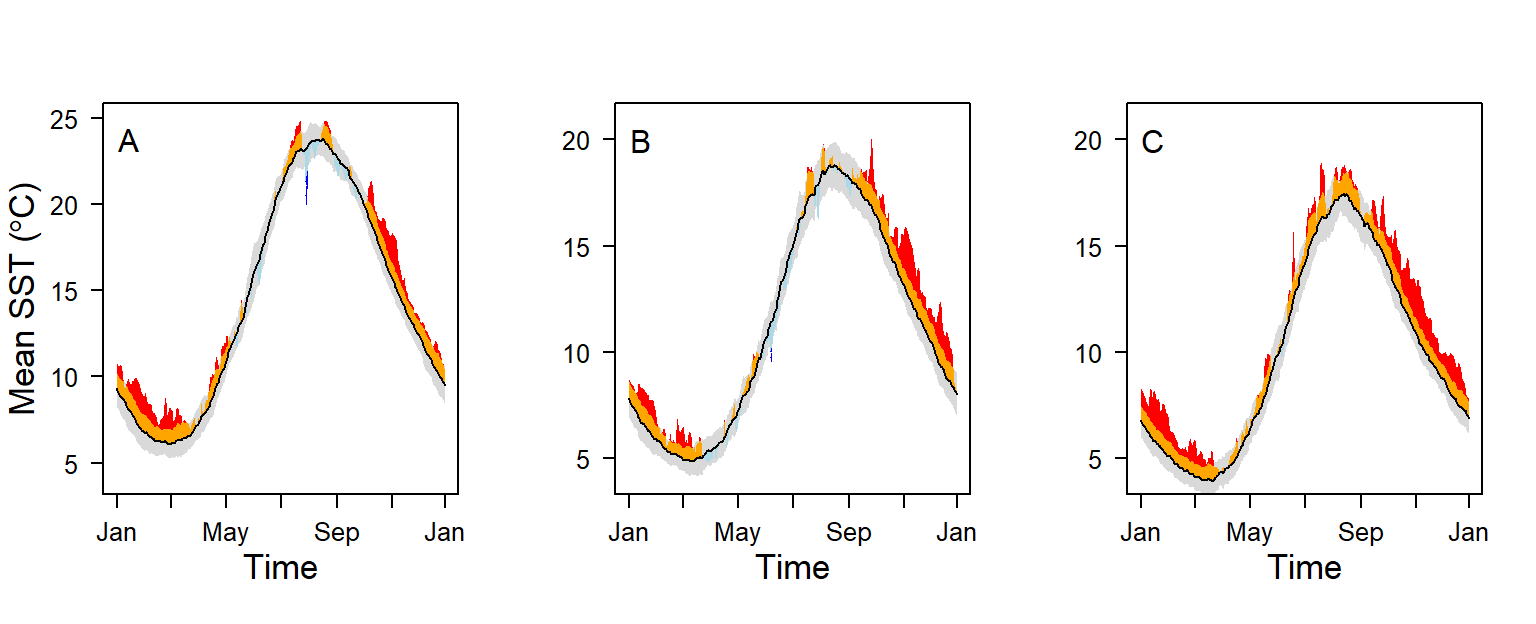
\includegraphics{C:/Users/kimberly.bastille/Desktop/tech-doc/imagesplotting-1} 

}

\caption{Long-term mean SSTs for the Mid-Atlantic Bight (A), Georges Bank (B), and Gulf of Maine (C). Orange and cyan shading show where the 2017 daily SST values were above or below the long-term mean respectively; red and dark blue shades indicate days when the 2017 mean exceeded +/- 1 standard deviation from the long-term mean.}\label{fig:plotting}
\end{figure}

\chapter{Aquaculture}\label{aquaculture}

\textbf{Description}: Aquaculture indicators

\textbf{Found in}: State of the Ecosystem - Gulf of Maine \& Georges
Bank (2017, 2018), State of the Ecosystem - Mid-Atlantic (2017, 2018,
2019)

\textbf{Indicator category}: Synthesis of published information

\textbf{Contributor(s)}: Sean Hardison, Lisa Calvo, Karl Roscher

\textbf{Data steward}: Sean Hardison
\href{mailto:sean.hardison@noaa.gov}{\nolinkurl{sean.hardison@noaa.gov}}

\textbf{Point of contact}: Sean Hardison
\href{mailto:sean.hardison@noaa.gov}{\nolinkurl{sean.hardison@noaa.gov}}

\textbf{Public availability statement}: Source data are publicly
available in referenced reports, and are also available for download
\href{https://comet.nefsc.noaa.gov/erddap/tabledap/aquaculture_soe_v1.html}{here}.

\section{Methods}\label{methods-2}

Aquaculture data included in the State of the Ecosystem (SOE) report
were time series of number of oysters sold in Virginia, Maryland, and
New Jersey.

\subsection{Data sources}\label{data-sources-2}

Virginia oyster harvest data are collected from mail and internet-based
surveys of active oyster aquaculture operations on both sides of the
Chesapeake Bay, which are then synthesized in an annual report (Hudson
\protect\hyperlink{ref-Hudson2017a}{2017}). In Maryland, shellfish
aquaculturists are required to report their monthly harvests to the
Maryland Department of Natural Resources (MD-DNR). The MD-DNR then
aggregates the harvest data for release in the Maryland Aquaculture
Coordinating Council Annual Report (ACC
\protect\hyperlink{ref-ACC2017}{2017}), from which data were collected.
Similar to Virginia, New Jersey releases annual reports synthesizing
electronic survey results from lease-holding shellfish growers. Data
from New Jersey reflects cage reared oysters grown from hatchery seed
(Calvo \protect\hyperlink{ref-Calvo2017}{2017}).

\subsection{Data extraction}\label{data-extraction-2}

Data were collected directly from state aquaculture reports. Oyster
harvest data in MD was reported in bushels which were then converted to
individual oysters by an estimate of 300 oysters bushel\(^{-1}\). View
processing code for this indicator
\href{https://github.com/NOAA-EDAB/ecodata/blob/master/data-raw/get_aquaculture.R}{here}.

\subsection{Data analysis}\label{data-analysis-1}

No data analyses occurred for this indicator.

\subsection{Data processing}\label{data-processing}

Aquaculture data were formatted for inclusion in the ecodata R package
using the following R code.

\begin{Shaded}
\begin{Highlighting}[]
\CommentTok{#Processing code for oyster harvest data in the Mid-Atlantic}

\CommentTok{#These data were collected directly from shellfish aquaculture surveys performed by state agencies and}
\CommentTok{#universities. }

\CommentTok{#NJ: http://njseagrant.org/new-jersey-shellfish-aquaculture-situation-outlook-report-new/}
\CommentTok{#VA: http://www.vims.edu/research/units/centerspartners/map/aquaculture/docs_aqua/vims_mrr_2018-9.pdf}
\CommentTok{#MD: Data from MD Aquaculture Coordinating Council meeting reports. Newest reports available upon request}

\KeywordTok{library}\NormalTok{(dplyr)}
\KeywordTok{library}\NormalTok{(tidyr)}

\NormalTok{raw.dir <-}\StringTok{ }\NormalTok{here}\OperatorTok{::}\KeywordTok{here}\NormalTok{(}\StringTok{"data-raw"}\NormalTok{)}

\NormalTok{get_aquaculture <-}\StringTok{ }\ControlFlowTok{function}\NormalTok{(}\DataTypeTok{save_clean =}\NormalTok{ F)\{}
\NormalTok{  aquaculture <-}\StringTok{ }\KeywordTok{read.csv}\NormalTok{(}\KeywordTok{file.path}\NormalTok{(raw.dir,}\StringTok{"mab_oyster_harvest.csv"}\NormalTok{))}
  
  \ControlFlowTok{if}\NormalTok{ (save_clean)\{}
\NormalTok{    usethis}\OperatorTok{::}\KeywordTok{use_data}\NormalTok{(aquaculture, }\DataTypeTok{overwrite =}\NormalTok{ T)}
\NormalTok{  \} }\ControlFlowTok{else}\NormalTok{ \{}
    \KeywordTok{return}\NormalTok{(aquaculture)}
\NormalTok{  \}}
  
\NormalTok{\}}
\end{Highlighting}
\end{Shaded}

\subsection{Plotting}\label{plotting-1}

\begin{Shaded}
\begin{Highlighting}[]
\NormalTok{aqua <-}\StringTok{ }\NormalTok{ecodata}\OperatorTok{::}\NormalTok{aquaculture }\OperatorTok\StringTok{ }
\StringTok{  }\KeywordTok{group_by}\NormalTok{(Var) }\OperatorTok\StringTok{ }
\StringTok{  }\KeywordTok{mutate}\NormalTok{(}\DataTypeTok{hline =} \KeywordTok{mean}\NormalTok{(Value)) }\OperatorTok
\StringTok{  }\KeywordTok{ungroup}\NormalTok{() }\OperatorTok\StringTok{ }
\StringTok{  }\KeywordTok{mutate}\NormalTok{(}\DataTypeTok{Var =}\NormalTok{ plyr}\OperatorTok{::}\KeywordTok{mapvalues}\NormalTok{(Var, }\DataTypeTok{from =} \KeywordTok{c}\NormalTok{(}\StringTok{"md oyster harvest"}\NormalTok{,}\StringTok{"nj oyster harvest"}\NormalTok{,}\StringTok{"va oyster harvest"}\NormalTok{),}
                                                    \DataTypeTok{to  =} \KeywordTok{c}\NormalTok{(}\StringTok{"MD"}\NormalTok{,}\StringTok{"NJ"}\NormalTok{,}\StringTok{"VA"}\NormalTok{))) }\OperatorTok
\StringTok{  }\NormalTok{dplyr}\OperatorTok{::}\KeywordTok{rename}\NormalTok{(}\DataTypeTok{State =}\NormalTok{ Var)}

\NormalTok{aqua}\OperatorTok{$}\NormalTok{State <-}\StringTok{ }\KeywordTok{factor}\NormalTok{(aqua}\OperatorTok{$}\NormalTok{State, }\DataTypeTok{levels =} \KeywordTok{c}\NormalTok{(}\StringTok{"VA"}\NormalTok{,}\StringTok{"MD"}\NormalTok{,}\StringTok{"NJ"}\NormalTok{))}


\KeywordTok{ggplot}\NormalTok{() }\OperatorTok{+}\StringTok{ }
\StringTok{  }\KeywordTok{geom_segment}\NormalTok{(}\KeywordTok{aes}\NormalTok{(}\DataTypeTok{x=}\DecValTok{2005}\NormalTok{,}\DataTypeTok{xend=}\DecValTok{2017}\NormalTok{,}\DataTypeTok{y=}\KeywordTok{mean}\NormalTok{(aquaculture[aquaculture}\OperatorTok{$}\NormalTok{Var }\OperatorTok{==}\StringTok{ "va oyster harvest"}\NormalTok{,]}\OperatorTok{$}\NormalTok{Value),}
                   \DataTypeTok{yend=}\KeywordTok{mean}\NormalTok{(aquaculture[aquaculture}\OperatorTok{$}\NormalTok{Var }\OperatorTok{==}\StringTok{ "va oyster harvest"}\NormalTok{,]}\OperatorTok{$}\NormalTok{Value)),}
               \DataTypeTok{size =}\NormalTok{ hline.size,}
           \DataTypeTok{alpha =}\NormalTok{ hline.alpha,}
           \DataTypeTok{linetype =}\NormalTok{ hline.lty,}
           \DataTypeTok{color =} \StringTok{"#1b9e77"}\NormalTok{,}
           \DataTypeTok{inherit.aes =}\NormalTok{ F) }\OperatorTok{+}
\StringTok{  }\KeywordTok{geom_segment}\NormalTok{(}\KeywordTok{aes}\NormalTok{(}\DataTypeTok{x=}\DecValTok{2012}\NormalTok{,}\DataTypeTok{xend=}\DecValTok{2016}\NormalTok{,}\DataTypeTok{y=}\KeywordTok{mean}\NormalTok{(aquaculture[aquaculture}\OperatorTok{$}\NormalTok{Var }\OperatorTok{==}\StringTok{ "nj oyster harvest"}\NormalTok{,]}\OperatorTok{$}\NormalTok{Value),}
                   \DataTypeTok{yend=}\KeywordTok{mean}\NormalTok{(aquaculture[aquaculture}\OperatorTok{$}\NormalTok{Var }\OperatorTok{==}\StringTok{ "nj oyster harvest"}\NormalTok{,]}\OperatorTok{$}\NormalTok{Value)),}
               \DataTypeTok{size =}\NormalTok{ hline.size,}
           \DataTypeTok{alpha =}\NormalTok{ hline.alpha,}
           \DataTypeTok{linetype =}\NormalTok{ hline.lty,}
           \DataTypeTok{color =} \StringTok{"#d95f02"}\NormalTok{,}
           \DataTypeTok{inherit.aes =}\NormalTok{ F) }\OperatorTok{+}
\StringTok{  }\KeywordTok{geom_segment}\NormalTok{(}\KeywordTok{aes}\NormalTok{(}\DataTypeTok{x=}\DecValTok{2012}\NormalTok{,}\DataTypeTok{xend=}\DecValTok{2017}\NormalTok{,}\DataTypeTok{y=}\KeywordTok{mean}\NormalTok{(aquaculture[aquaculture}\OperatorTok{$}\NormalTok{Var }\OperatorTok{==}\StringTok{ "md oyster harvest"}\NormalTok{,]}\OperatorTok{$}\NormalTok{Value),}
                   \DataTypeTok{yend=}\KeywordTok{mean}\NormalTok{(aquaculture[aquaculture}\OperatorTok{$}\NormalTok{Var }\OperatorTok{==}\StringTok{ "md oyster harvest"}\NormalTok{,]}\OperatorTok{$}\NormalTok{Value)),}
               \DataTypeTok{size =}\NormalTok{ hline.size,}
           \DataTypeTok{alpha =}\NormalTok{ hline.alpha,}
           \DataTypeTok{linetype =}\NormalTok{ hline.lty,}
           \DataTypeTok{color =} \StringTok{"#7570b3"}\NormalTok{,}
           \DataTypeTok{inherit.aes =}\NormalTok{ F) }\OperatorTok{+}
\StringTok{ }\CommentTok{#Highlight last ten years}
\StringTok{  }\KeywordTok{geom_line}\NormalTok{(}\DataTypeTok{data =}\NormalTok{ aqua, }\KeywordTok{aes}\NormalTok{(}\DataTypeTok{x =}\NormalTok{ Time, }\DataTypeTok{y =}\NormalTok{ Value, }\DataTypeTok{color =}\NormalTok{ State), }\DataTypeTok{size =}\NormalTok{ lwd) }\OperatorTok{+}
\StringTok{  }\KeywordTok{geom_point}\NormalTok{(}\DataTypeTok{data =}\NormalTok{ aqua,}\KeywordTok{aes}\NormalTok{(}\DataTypeTok{x =}\NormalTok{ Time, }\DataTypeTok{y =}\NormalTok{ Value, }\DataTypeTok{color =}\NormalTok{ State), }\DataTypeTok{size =}\NormalTok{ pcex) }\OperatorTok{+}
\StringTok{  }\KeywordTok{scale_color_manual}\NormalTok{(}\DataTypeTok{values =} \KeywordTok{c}\NormalTok{(}\DataTypeTok{VA =} \StringTok{"#1b9e77"}\NormalTok{, }\DataTypeTok{MD =} \StringTok{"#7570b3"}\NormalTok{,}\DataTypeTok{NJ =} \StringTok{"#d95f02"}\NormalTok{)) }\OperatorTok{+}
\StringTok{  }\KeywordTok{scale_x_continuous}\NormalTok{(}\DataTypeTok{breaks =} \KeywordTok{seq}\NormalTok{(}\DecValTok{2005}\NormalTok{,}\DecValTok{2018}\NormalTok{,}\DecValTok{3}\NormalTok{),}\DataTypeTok{expand =} \KeywordTok{c}\NormalTok{(}\FloatTok{0.01}\NormalTok{, }\FloatTok{0.01}\NormalTok{)) }\OperatorTok{+}
\StringTok{  }\KeywordTok{scale_y_continuous}\NormalTok{(}\DataTypeTok{labels =} \ControlFlowTok{function}\NormalTok{(l)\{trans =}\StringTok{ }\NormalTok{l }\OperatorTok{/}\StringTok{ }\DecValTok{1000000}\NormalTok{\})}\OperatorTok{+}
\StringTok{  }\KeywordTok{ggtitle}\NormalTok{(}\StringTok{"Oyster harvest"}\NormalTok{)}\OperatorTok{+}
\StringTok{  }\KeywordTok{ylab}\NormalTok{(}\KeywordTok{expression}\NormalTok{(}\StringTok{"Oysters sold (10"}\OperatorTok{^}\DecValTok{6}\OperatorTok{*}\StringTok{" n)"}\NormalTok{)) }\OperatorTok{+}
\StringTok{  }\KeywordTok{xlab}\NormalTok{(}\StringTok{""}\NormalTok{)}\OperatorTok{+}
\StringTok{  }\KeywordTok{theme_ts}\NormalTok{()}
\end{Highlighting}
\end{Shaded}

\begin{figure}

{\centering 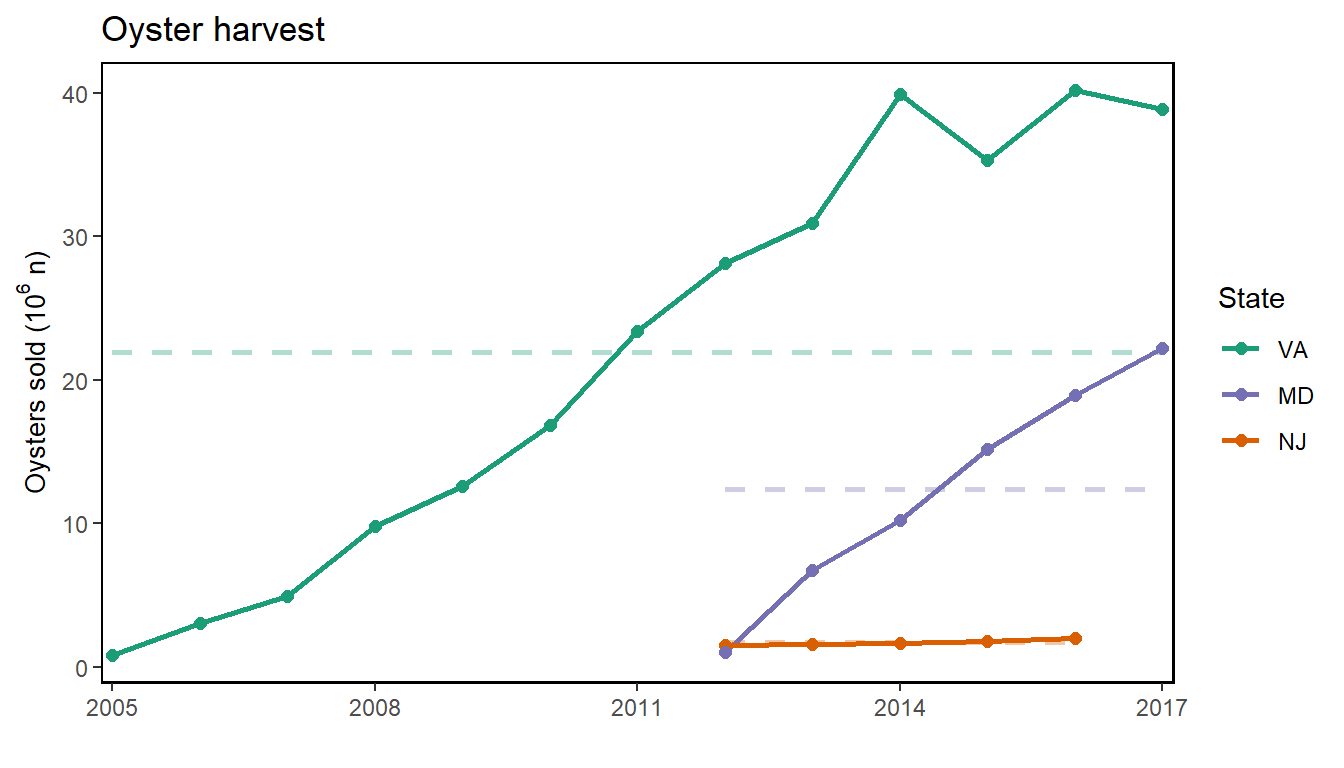
\includegraphics{C:/Users/kimberly.bastille/Desktop/tech-doc/imagesunnamed-chunk-4-1} 

}

\caption{Oyster aquaculture production in terms of number of oysters sold from Virginia, Maryland, and New Jersey.}\label{fig:unnamed-chunk-4}
\end{figure}

\chapter{Bennet Indicator}\label{bennet-indicator}

\textbf{Description}: Bennet Indicator

\textbf{Found in}: State of the Ecosystem - Gulf of Maine \& Georges
Bank (2018, 2019), State of the Ecosystem - Mid-Atlantic (2018, 2019)

\textbf{Indicator category}: Database pull with analysis

\textbf{Contributor(s)}: John Walden

\textbf{Data steward}: Sean Hardison,
\href{mailto:sean.hardison@noaa.gov}{\nolinkurl{sean.hardison@noaa.gov}}

\textbf{Point of contact}: John Walden,
\href{mailto:john.walden@noaa.gov}{\nolinkurl{john.walden@noaa.gov}}

\textbf{Public availability statement}: Derived CFDBS data are available
for this analysis (see \protect\hyperlink{comdat}{Comland}).

\section{Methods}\label{methods-3}

\subsection{Data sources}\label{data-sources-3}

Data used in the Bennet Indicator were derived from the Comland data
set; a processed subset of the Commercial Fisheries Database System
(CFDBS). The derived Comland data set is available for download
\href{https://comet.nefsc.noaa.gov/erddap/tabledap/group_landings_soe_v1.html}{here}.

\subsection{Data extraction}\label{data-extraction-3}

For information regarding processing of CFDBS, please see
\protect\hyperlink{comdat}{Comland} methods. The Comland dataset
containing seafood landings data was subsetted to US landings after 1964
where revenue was \(\geq\) 0 for each Ecological Production Unit
(i.e.~Mid-Atlantic Bight, Georges Bank, and Gulf of Maine). Each EPU was
run in an individual R script, and the code specific to Georges Bank is
shown below.

\begin{Shaded}
\begin{Highlighting}[]
\CommentTok{#This code is used to load and process comland data. See comland methods for source data (CFDBS) processing methods. }

\NormalTok{drake}\OperatorTok{::}\KeywordTok{readd}\NormalTok{(proc_get_mass_inshore_survey.R)}

\CommentTok{#Packages}
\NormalTok{PKG <-}\StringTok{ }\KeywordTok{c}\NormalTok{(}\StringTok{"data.table"}\NormalTok{,}\StringTok{"plyr"}\NormalTok{,}\StringTok{"RColorBrewer"}\NormalTok{, }\StringTok{"ggplot2"}\NormalTok{,}\StringTok{"cowplot"}\NormalTok{,}\StringTok{"gridExtra"}\NormalTok{,}\StringTok{"grid"}\NormalTok{)}
\ControlFlowTok{for}\NormalTok{ (p }\ControlFlowTok{in}\NormalTok{ PKG) \{}
  \ControlFlowTok{if}\NormalTok{(}\OperatorTok{!}\KeywordTok{require}\NormalTok{(p,}\DataTypeTok{character.only =} \OtherTok{TRUE}\NormalTok{)) \{  }
    \KeywordTok{install.packages}\NormalTok{(p)}
    \KeywordTok{require}\NormalTok{(p,}\DataTypeTok{character.only =} \OtherTok{TRUE}\NormalTok{)\}}
\NormalTok{\}}
\CommentTok{# #Setting Save path}


\CommentTok{#load "comland" data - These data are unavailble due to PII concerns. See aggregated data load below}
\NormalTok{ecosys2<-}\KeywordTok{subset}\NormalTok{(comland, US}\OperatorTok{==}\StringTok{'TRUE'} \OperatorTok{&}\StringTok{ }\NormalTok{YEAR}\OperatorTok{>=}\DecValTok{1964} \OperatorTok{&}\StringTok{ }\NormalTok{SPPVALUE }\OperatorTok{>=}\DecValTok{0}\NormalTok{)}

\CommentTok{#Load species and PDT codes}
\KeywordTok{load}\NormalTok{(}\KeywordTok{file.path}\NormalTok{(data.dir, }\StringTok{"Species_codes.RData"}\NormalTok{))}

\CommentTok{#Set EPU}
\NormalTok{epu <-}\StringTok{ "GB"}

\CommentTok{#processing}
\NormalTok{spp<-}\KeywordTok{subset}\NormalTok{(spp, NESPP3}\OperatorTok{>}\DecValTok{0}\NormalTok{)}
\NormalTok{spp2<-}\KeywordTok{unique}\NormalTok{(spp[,}\KeywordTok{c}\NormalTok{(}\DecValTok{3}\NormalTok{,}\DecValTok{12}\NormalTok{)], }\DataTypeTok{by=}\StringTok{'NESPP3'}\NormalTok{)}
\NormalTok{spp2<-spp2[}\KeywordTok{which}\NormalTok{(}\OperatorTok{!}\KeywordTok{duplicated}\NormalTok{(spp2}\OperatorTok{$}\NormalTok{NESPP3)),]}
\NormalTok{sp_combine<-}\KeywordTok{merge}\NormalTok{(ecosys2, spp2, }\DataTypeTok{by=}\StringTok{"NESPP3"}\NormalTok{, }\DataTypeTok{all.x=}\OtherTok{TRUE}\NormalTok{)}
\NormalTok{add.apex <-}\StringTok{ }\KeywordTok{data.table}\NormalTok{(}\DataTypeTok{NESPP3 =} \DecValTok{000}\NormalTok{, }\DataTypeTok{YEAR =} \DecValTok{1971}\NormalTok{, }\DataTypeTok{QY =} \DecValTok{1}\NormalTok{, }\DataTypeTok{GEAR =} \StringTok{'other'}\NormalTok{,}
                       \DataTypeTok{SIZE =} \StringTok{'small'}\NormalTok{, }\DataTypeTok{EPU =}\NormalTok{ epu, }\DataTypeTok{UTILCD =} \DecValTok{0}\NormalTok{, }\DataTypeTok{SPPLIVMT =} \DecValTok{0}\NormalTok{,}
                       \DataTypeTok{SPPVALUE =} \DecValTok{0}\NormalTok{, }\DataTypeTok{US =} \OtherTok{TRUE}\NormalTok{, }\DataTypeTok{Feeding.guild =} \StringTok{'Apex Predator'}\NormalTok{)}
\NormalTok{sp_combine <-}\StringTok{ }\KeywordTok{rbindlist}\NormalTok{(}\KeywordTok{list}\NormalTok{(sp_combine, add.apex))}

\CommentTok{#Subset data into Georges Bank group}
\NormalTok{LANDINGS<-}\KeywordTok{subset}\NormalTok{(sp_combine)}
\NormalTok{LANDINGS<-LANDINGS[}\KeywordTok{which}\NormalTok{(}\OperatorTok{!}\KeywordTok{is.na}\NormalTok{(LANDINGS}\OperatorTok{$}\NormalTok{Feeding.guild)),]}

\CommentTok{#Set Up data Table}
\NormalTok{landsum<-}\KeywordTok{data.table}\NormalTok{(LANDINGS)}
\CommentTok{# setkey(landsum,  "EPU", "YEAR","Feeding.guild")}
\KeywordTok{setkey}\NormalTok{(landsum,}\StringTok{"EPU"}\NormalTok{,}\StringTok{"YEAR"}\NormalTok{,}\StringTok{"Feeding.guild"}\NormalTok{)}


\CommentTok{#Sum by feeding guild}
\NormalTok{landsum[,}\KeywordTok{lapply}\NormalTok{(.SD, sum, }\DataTypeTok{na.rm=}\OtherTok{TRUE}\NormalTok{), by=}\KeywordTok{key}\NormalTok{(landsum), .SDcols=}\KeywordTok{c}\NormalTok{(}\StringTok{"SPPLIVMT"}\NormalTok{,}\StringTok{"SPPVALUE"}\NormalTok{)]}
\end{Highlighting}
\end{Shaded}

\subsection{Data analysis}\label{data-analysis-2}

Revenue earned by harvesting resources from a Large Marine Ecosystem
(LME) at time \emph{t} is a function of both the quantity landed of each
species and the prices paid for landings. Changes in revenue between any
two years depends on both prices and quantities in each year, and both
may be changing simultaneously. For example, an increase in the harvest
of higher priced species, such as scallops can lead to an overall
increase in total revenue from an LME between time periods even if
quantities landed of other species decline. Although measurement of
revenue change is useful, the ability to see what drives revenue change,
whether it is changing harvest levels, the mix of species landed, or
price changes provides additional valuable information. Therefore, it is
useful to decompose revenue change into two parts, one which is due to
changing quantities (or volumes), and a second which is due to changing
prices. In an LME, the quantity component will yield useful information
about how the species mix of harvests are changing through time.

A Bennet indicator (BI) is used to examine revenue change between 1964
and 2015 for two major LME regions. It is composed of a volume indicator
(VI), which measures changes in quantities, and a price indicator (PI)
which measures changes in prices. The Bennet (1920) indicator (BI) was
first used to show how a change in social welfare could be decomposed
into a sum of a price and quantity change indicator (Cross and Färe
\protect\hyperlink{ref-Cross2009}{2009}). It is called an indicator
because it is based on differences in value between time periods, rather
than ratios, which are referred to as indices. The BI is the indicator
equivalent of the more popular Fisher index (Balk
\protect\hyperlink{ref-Balk2010}{2010}), and has been used to examine
revenue changes in Swedish pharmacies, productivity change in U.S.
railroads (Lim and Lovell \protect\hyperlink{ref-lim2009}{2009}), and
dividend changes in banking operations (Grifell-Tatjé and Lovell
\protect\hyperlink{ref-Grifell-Tatje2004}{2004}). An attractive feature
of the BI is that the overall indicator is equal to the sum of its
subcomponents (Balk \protect\hyperlink{ref-Balk2010}{2010}). This allows
one to examine what component of overall revenue is responsible for
change between time periods. This allows us to examine whether changing
quantities or prices of separate species groups are driving revenue
change in each EPU between 1964 and 2015.

Revenue in a given year for any species group is the product of quantity
landed times price, and the sum of revenue from all groups is total
revenue from the LME. In any year, both prices and quantities can change
from prior years, leading to total revenue change. At time t, revenue
(R) is defined as \[R^{t} = \sum_{j=1}^{J}p_{j}^{t}y_{j}^{t},\] where
\(p_{j}\) is the price for species group \(j\), and \(y_{j}\) is the
quantity landed of species group \(j\). Revenue change between any two
time periods, say \(t+1\) and \(t\), is then \(R^{t+1}-R^{t}\), which
can also be expressed as:
\[\Delta R = \sum_{j=1}^{J}p_{j}^{t+1}y_{j}^{t+1}-\sum_{j=1}^{J}p_{j}^{t}y_{j}^{t}.\]
This change can be decomposed further, yielding a VI and PI. The VI is
calculated using the following formula (Georgianna, Lee, and Walden
\protect\hyperlink{ref-Georgianna2017}{2017}):

\[VI = \frac{1}{2}(\sum_{j=1}^{J}p_{j}^{t+1}y_{j}^{t+1} - \sum_{j=1}^{J}p_{j}^{t+1}y_{j}^{t} + \sum_{j=1}^{J}p_{j}^{t}y_{j}^{t+1} - \sum_{j=1}^{J}p_{j}^{t}y_{j}^{t})\]
The price indicator (PI) is calculated as follows:
\[PI = \frac{1}{2}(\sum_{j=1}^{J}y_{j}^{t+1}p_{j}^{t+1} - \sum_{j=1}^{J}y_{j}^{t+1}p_{j}^{t} + \sum_{j=1}^{J}y_{j}^{t}p_{j}^{t+1} - \sum_{j=1}^{J}y_{j}^{t}p_{j}^{t})\]
Total revenue change between time \(t\) and \(t+1\) is the sum of the VI
and PI. Since revenue change is being driven by changes in the
individual prices and quantities landed of each species group, changes
at the species group level can be examined separately by taking
advantage of the additive property of the indicator. For example, if
there are five different species groups, the sum of the VI for each
group will equal the overall VI, and the sum of the PI for each group
will equal the overall PI.

\begin{Shaded}
\begin{Highlighting}[]
\CommentTok{#R code to construct Bennet Indicator for Ecosystem Project}
\CommentTok{#Author: John Walden}
\CommentTok{#Date: October 4, 2017}
\CommentTok{#}
\CommentTok{#Revised January 18, 2018 to calculate the indicator relative to average conditions}
\CommentTok{#during each time period. Set EPU in extraction/processing code chunk above.}


\CommentTok{#filter by specific EPU}
\NormalTok{epu =}\StringTok{ "GB"}
\NormalTok{value <-}\StringTok{ }\KeywordTok{subset}\NormalTok{(landsum, EPU }\OperatorTok{==}\StringTok{ }\NormalTok{epu)}

\CommentTok{#Calculate price}
\NormalTok{value}\OperatorTok{$}\NormalTok{PRICE=value}\OperatorTok{$}\NormalTok{SPPVALUE}\OperatorTok{/}\NormalTok{value}\OperatorTok{$}\NormalTok{SPPLIVMT}
\NormalTok{value[}\KeywordTok{is.na}\NormalTok{(value)]<-}\DecValTok{0}


\CommentTok{#Next two lines are to calculate mean values for landings}
\CommentTok{#and value for the time series by feeding guild}

\NormalTok{meanval<-}\KeywordTok{as.data.frame}\NormalTok{(value[,}\DataTypeTok{j=}\KeywordTok{list}\NormalTok{(}\KeywordTok{mean}\NormalTok{(SPPVALUE,}\DataTypeTok{na.rm=}\OtherTok{TRUE}\NormalTok{), }\KeywordTok{mean}\NormalTok{(SPPLIVMT,}\DataTypeTok{na.rm=}\OtherTok{TRUE}\NormalTok{)), }\DataTypeTok{by=}\NormalTok{Feeding.guild])}
\NormalTok{meanval<-}\KeywordTok{rename}\NormalTok{(meanval, }\KeywordTok{c}\NormalTok{(}\StringTok{"V1"}\NormalTok{=}\StringTok{"BASEV"}\NormalTok{, }\StringTok{"V2"}\NormalTok{=}\StringTok{"BASEQ"}\NormalTok{))}
\NormalTok{meanval}\OperatorTok{$}\NormalTok{BASEP=meanval}\OperatorTok{$}\NormalTok{BASEV}\OperatorTok{/}\NormalTok{meanval}\OperatorTok{$}\NormalTok{BASEQ;}

\CommentTok{#order by feeding guild}

\NormalTok{value<-value[}\KeywordTok{order}\NormalTok{(value}\OperatorTok{$}\NormalTok{Feeding.guild),]}
\NormalTok{meanval<-meanval[}\KeywordTok{order}\NormalTok{(meanval}\OperatorTok{$}\NormalTok{Feeding.guild),]}

\CommentTok{#Merge Value data frame with Base Year Value Data Frame}
\NormalTok{value<-}\KeywordTok{merge}\NormalTok{(value, meanval, }\DataTypeTok{by=}\StringTok{"Feeding.guild"}\NormalTok{)}

\CommentTok{#Construct price and Volume Indicators}
\CommentTok{#NOTE: ALL values are normalized to $1,000,000}

\NormalTok{value}\OperatorTok{$}\NormalTok{VI=((}\FloatTok{0.5}\OperatorTok{*}\NormalTok{(value}\OperatorTok{$}\NormalTok{BASEP}\OperatorTok{+}\NormalTok{value}\OperatorTok{$}\NormalTok{PRICE))}\OperatorTok{*}\NormalTok{(value}\OperatorTok{$}\NormalTok{SPPLIVMT}\OperatorTok{-}\NormalTok{value}\OperatorTok{$}\NormalTok{BASEQ))}\OperatorTok{/}\DecValTok{1000000}
\NormalTok{value}\OperatorTok{$}\NormalTok{PI=((}\FloatTok{0.5}\OperatorTok{*}\NormalTok{(value}\OperatorTok{$}\NormalTok{BASEQ}\OperatorTok{+}\NormalTok{value}\OperatorTok{$}\NormalTok{SPPLIVMT))}\OperatorTok{*}\NormalTok{(value}\OperatorTok{$}\NormalTok{PRICE}\OperatorTok{-}\NormalTok{value}\OperatorTok{$}\NormalTok{BASEP))}\OperatorTok{/}\DecValTok{1000000}

\NormalTok{value<-value[}\KeywordTok{order}\NormalTok{(value}\OperatorTok{$}\NormalTok{YEAR),]}

\CommentTok{#The next Data table sets up the yearly aggregate Bennet PI and VI}

\NormalTok{biyear<-}\KeywordTok{data.table}\NormalTok{(value)}
\KeywordTok{setkey}\NormalTok{(biyear, }\StringTok{"YEAR"}\NormalTok{)}
\NormalTok{biyear<-biyear[,}\KeywordTok{lapply}\NormalTok{(.SD, sum), by=}\KeywordTok{key}\NormalTok{(biyear), .SDcols=}\KeywordTok{c}\NormalTok{(}\StringTok{"VI"}\NormalTok{,}\StringTok{"PI"}\NormalTok{,}\StringTok{"BASEV"}\NormalTok{,}\StringTok{"SPPVALUE"}\NormalTok{)]}
\NormalTok{biyear}\OperatorTok{$}\NormalTok{revchange<-(biyear}\OperatorTok{$}\NormalTok{VI}\OperatorTok{+}\NormalTok{biyear}\OperatorTok{$}\NormalTok{PI)}
\NormalTok{biyear}\OperatorTok{$}\NormalTok{BI<-(biyear}\OperatorTok{$}\NormalTok{VI }\OperatorTok{+}\StringTok{ }\NormalTok{biyear}\OperatorTok{$}\NormalTok{PI)}

\CommentTok{#The Next Steps restructure the year data frame so the yearly}
\CommentTok{#Bennet Indicator can be plotted. Negative values are difficult in GGPLOT.}
\CommentTok{#Since the Bennet indicator can have a negative value, separate data frames}
\CommentTok{#need to be created. First, the data needs to be restructured to use the }
\CommentTok{#stacked bar function in ggplot. GGPLOT is used because it can graph differen#t data layers on the same graph.}

\NormalTok{y1<-biyear[,}\KeywordTok{c}\NormalTok{(}\DecValTok{1}\NormalTok{,}\DecValTok{2}\NormalTok{)]}
\NormalTok{y1}\OperatorTok{$}\NormalTok{indicator=}\StringTok{'VI'}
\NormalTok{y2<-biyear[,}\KeywordTok{c}\NormalTok{(}\DecValTok{1}\NormalTok{,}\DecValTok{3}\NormalTok{)]}
\NormalTok{y2}\OperatorTok{$}\NormalTok{indicator=}\StringTok{'PI'}

\KeywordTok{colnames}\NormalTok{(y1)[}\DecValTok{2}\NormalTok{]<-}\StringTok{"value"}
\KeywordTok{colnames}\NormalTok{(y2)[}\DecValTok{2}\NormalTok{]<-}\StringTok{"value"}
\NormalTok{ytotal<-}\KeywordTok{rbind}\NormalTok{(y1,y2)}
\end{Highlighting}
\end{Shaded}

\subsection{Data processing}\label{data-processing-1}

Bennet indicator time series were formatted for inclusion in the ecodata
R package using the following R code.

\begin{Shaded}
\begin{Highlighting}[]
\CommentTok{# Process Bennet indicator; price and volume indicators}

\KeywordTok{library}\NormalTok{(dplyr)}
\KeywordTok{library}\NormalTok{(tidyr)}
\KeywordTok{library}\NormalTok{(magrittr)}

\NormalTok{raw.dir <-}\StringTok{ }\NormalTok{here}\OperatorTok{::}\KeywordTok{here}\NormalTok{(}\StringTok{'inst'}\NormalTok{,}\StringTok{'extdata'}\NormalTok{)}

\NormalTok{get_bennet <-}\StringTok{ }\ControlFlowTok{function}\NormalTok{(}\DataTypeTok{save_clean =}\NormalTok{ F)\{}
  
  \CommentTok{# Find relevant files and load them into workspace}
\NormalTok{  files =}\StringTok{ }\KeywordTok{list.files}\NormalTok{(raw.dir, }\DataTypeTok{pattern=}\StringTok{"_vi|_pi|_bennet"}\NormalTok{)}
  \ControlFlowTok{for}\NormalTok{ (i }\ControlFlowTok{in} \DecValTok{1}\OperatorTok{:}\KeywordTok{length}\NormalTok{(files)) }\KeywordTok{assign}\NormalTok{(files[i], }\KeywordTok{read.csv}\NormalTok{(}\KeywordTok{file.path}\NormalTok{(raw.dir,files[i])))}
  
  \CommentTok{#Process Bennet indicator data aggregated to the level of EPU (all feeding guilds)}
\NormalTok{  bennet <-}\StringTok{ }\OtherTok{NULL}
  \ControlFlowTok{for}\NormalTok{ (i }\ControlFlowTok{in} \KeywordTok{ls}\NormalTok{())\{}
    \ControlFlowTok{if}\NormalTok{ (stringr}\OperatorTok{::}\KeywordTok{str_detect}\NormalTok{(i, }\StringTok{"_bennet_"}\NormalTok{))\{}
\NormalTok{      epu <-}\StringTok{ }\NormalTok{stringr}\OperatorTok{::}\KeywordTok{str_extract}\NormalTok{(i, }\StringTok{"gb|gom|mab"}\NormalTok{) }\CommentTok{#Extract EPU}
      
      \CommentTok{#Process into SOE format}
\NormalTok{      out <-}\StringTok{ }\KeywordTok{get}\NormalTok{(i) }\OperatorTok\StringTok{ }\KeywordTok{mutate}\NormalTok{(}\DataTypeTok{EPU =}\NormalTok{ epu,}
                               \DataTypeTok{Units =} \StringTok{"million USD ($2015)"}\NormalTok{) }\OperatorTok
\StringTok{        }\NormalTok{dplyr}\OperatorTok{::}\KeywordTok{select}\NormalTok{(}\OperatorTok{-}\NormalTok{X) }\OperatorTok
\StringTok{        }\KeywordTok{gather}\NormalTok{(.,Var, Value,}\OperatorTok{-}\NormalTok{YEAR,}\OperatorTok{-}\NormalTok{EPU, }\OperatorTok{-}\NormalTok{Units) }\OperatorTok
\StringTok{        }\KeywordTok{mutate}\NormalTok{(}\DataTypeTok{Var =} \KeywordTok{paste}\NormalTok{(Var, }\StringTok{"EPU aggregate"}\NormalTok{),}
               \DataTypeTok{EPU =} \KeywordTok{toupper}\NormalTok{(EPU)) }\OperatorTok
\StringTok{        }\NormalTok{dplyr}\OperatorTok{::}\KeywordTok{rename}\NormalTok{(}\DataTypeTok{Time =}\NormalTok{ YEAR) }\OperatorTok\StringTok{ }
\StringTok{        }\KeywordTok{as.data.frame}\NormalTok{()}
      
      \KeywordTok{assign}\NormalTok{(}\StringTok{'bennet'}\NormalTok{,}\KeywordTok{rbind}\NormalTok{(bennet, out))}
      
\NormalTok{    \}}
\NormalTok{  \}}
  
\NormalTok{  pi.vi <-}\StringTok{ }\OtherTok{NULL}
  
  \ControlFlowTok{for}\NormalTok{ (i }\ControlFlowTok{in} \KeywordTok{ls}\NormalTok{())\{}
    \ControlFlowTok{if}\NormalTok{ (stringr}\OperatorTok{::}\KeywordTok{str_detect}\NormalTok{(i, }\StringTok{"_pi|_vi"}\NormalTok{))\{}
\NormalTok{      epu <-}\StringTok{ }\NormalTok{stringr}\OperatorTok{::}\KeywordTok{str_extract}\NormalTok{(i, }\StringTok{"gb|gom|mab"}\NormalTok{)}
\NormalTok{      indicator <-}\StringTok{ }\NormalTok{stringr}\OperatorTok{::}\KeywordTok{str_extract}\NormalTok{(i, }\StringTok{"vi|pi"}\NormalTok{)}
      
\NormalTok{      out <-}\StringTok{ }\KeywordTok{get}\NormalTok{(i) }\OperatorTok
\StringTok{        }\KeywordTok{mutate}\NormalTok{(}\DataTypeTok{EPU =} \KeywordTok{toupper}\NormalTok{(epu),}
               \DataTypeTok{class =} \KeywordTok{toupper}\NormalTok{(indicator),}
               \DataTypeTok{Units =} \StringTok{"million USD ($2015)"}\NormalTok{) }\OperatorTok
\StringTok{        }\KeywordTok{gather}\NormalTok{(.,Var,Value,}\OperatorTok{-}\NormalTok{YEAR, }\OperatorTok{-}\NormalTok{class, }\OperatorTok{-}\NormalTok{EPU,}\OperatorTok{-}\NormalTok{Units) }\OperatorTok\StringTok{ }
\StringTok{        }\KeywordTok{unite}\NormalTok{(., }\StringTok{"Var"}\NormalTok{, }\KeywordTok{c}\NormalTok{(}\StringTok{"Var"}\NormalTok{,}\StringTok{"class"}\NormalTok{), }\DataTypeTok{sep =} \StringTok{" "}\NormalTok{) }\OperatorTok\StringTok{ }
\StringTok{        }\NormalTok{dplyr}\OperatorTok{::}\KeywordTok{rename}\NormalTok{(}\DataTypeTok{Time =}\NormalTok{ YEAR) }\OperatorTok\StringTok{ }
\StringTok{        }\KeywordTok{as.data.frame}\NormalTok{()}
      
      \KeywordTok{assign}\NormalTok{(}\StringTok{'pi.vi'}\NormalTok{, }\KeywordTok{rbind}\NormalTok{(pi.vi, out))}
      
\NormalTok{    \}}
\NormalTok{  \}}
  
\NormalTok{  bennet <-}\StringTok{ }\KeywordTok{rbind}\NormalTok{(pi.vi, bennet)}
  
  \ControlFlowTok{if}\NormalTok{ (save_clean)\{}
\NormalTok{    usethis}\OperatorTok{::}\KeywordTok{use_data}\NormalTok{(bennet, }\DataTypeTok{overwrite =}\NormalTok{ T)}
\NormalTok{  \} }\ControlFlowTok{else}\NormalTok{ \{}
    \KeywordTok{return}\NormalTok{(bennet)}
\NormalTok{  \}}
  
\NormalTok{\}}
\end{Highlighting}
\end{Shaded}

\subsection{Plotting}\label{plotting-2}

\begin{Shaded}
\begin{Highlighting}[]
\CommentTok{#Filter data into two dataframes for plotting}
\NormalTok{indicators <-}\StringTok{ }\NormalTok{ecodata}\OperatorTok{::}\NormalTok{bennet }\OperatorTok\StringTok{ }
\StringTok{  }\KeywordTok{filter}\NormalTok{(EPU }\OperatorTok{==}\StringTok{ "MAB"}\NormalTok{,}
\NormalTok{         Var }\OperatorTok\StringTok{ }\KeywordTok{c}\NormalTok{(}\StringTok{"VI EPU aggregate"}\NormalTok{,}
                    \StringTok{"PI EPU aggregate"}\NormalTok{)) }\OperatorTok\StringTok{ }
\StringTok{  }\KeywordTok{mutate}\NormalTok{(Var, }\DataTypeTok{Var =}\NormalTok{ plyr}\OperatorTok{::}\KeywordTok{mapvalues}\NormalTok{(Var, }\DataTypeTok{from =} \KeywordTok{c}\NormalTok{(}\StringTok{"VI EPU aggregate"}\NormalTok{,}\StringTok{"PI EPU aggregate"}\NormalTok{),}
                                    \DataTypeTok{to =} \KeywordTok{c}\NormalTok{(}\StringTok{"Volume"}\NormalTok{,}\StringTok{"Price"}\NormalTok{)))}

\NormalTok{revchange <-}\StringTok{ }\NormalTok{ecodata}\OperatorTok{::}\NormalTok{bennet }\OperatorTok\StringTok{ }
\StringTok{  }\KeywordTok{filter}\NormalTok{(EPU }\OperatorTok{==}\StringTok{ "MAB"}\NormalTok{,}
\NormalTok{         Var }\OperatorTok\StringTok{ }\KeywordTok{c}\NormalTok{(}\StringTok{"REVCHANGE EPU aggregate"}\NormalTok{))}

\CommentTok{#custom bar fill color (color-blind friendly)}
\NormalTok{ind_fill <-}\StringTok{ }\KeywordTok{c}\NormalTok{(}\StringTok{"#a6cee3"}\NormalTok{, }\StringTok{"#b2df8a"}\NormalTok{)}

\CommentTok{#limits}
\NormalTok{y.lim <-}\StringTok{ }\KeywordTok{c}\NormalTok{(}\OperatorTok{-}\DecValTok{450}\NormalTok{,}\DecValTok{450}\NormalTok{)}

\CommentTok{#plot}
\KeywordTok{ggplot}\NormalTok{(}\DataTypeTok{data =}\NormalTok{ indicators)}\OperatorTok{+}
\StringTok{  }
\StringTok{  }\CommentTok{#Highlight last ten years}
\StringTok{  }\KeywordTok{annotate}\NormalTok{(}\StringTok{"rect"}\NormalTok{, }\DataTypeTok{fill =}\NormalTok{ shade.fill, }\DataTypeTok{alpha =}\NormalTok{ shade.alpha,}
      \DataTypeTok{xmin =}\NormalTok{ x.shade.min , }\DataTypeTok{xmax =}\NormalTok{ x.shade.max,}
      \DataTypeTok{ymin =} \OperatorTok{-}\OtherTok{Inf}\NormalTok{, }\DataTypeTok{ymax =} \OtherTok{Inf}\NormalTok{)}\OperatorTok{+}
\StringTok{  }
\StringTok{  }\KeywordTok{geom_bar}\NormalTok{(}\KeywordTok{aes}\NormalTok{(}\DataTypeTok{x=}\NormalTok{Time, }\DataTypeTok{y=}\NormalTok{ Value, }\DataTypeTok{fill =}\NormalTok{ Var), }\DataTypeTok{stat=}\StringTok{"identity"}\NormalTok{)}\OperatorTok{+}
\StringTok{  }\KeywordTok{scale_fill_manual}\NormalTok{(}\DataTypeTok{name =} \StringTok{"Indicators"}\NormalTok{, }\DataTypeTok{values =}\NormalTok{ ind_fill) }\OperatorTok{+}
\StringTok{  }\KeywordTok{geom_line}\NormalTok{(}\DataTypeTok{data =}\NormalTok{ revchange, }\KeywordTok{aes}\NormalTok{(}\DataTypeTok{x =}\NormalTok{ Time, }\DataTypeTok{y =}\NormalTok{ Value, }\DataTypeTok{colour=}\StringTok{"$"}\NormalTok{))}\OperatorTok{+}
\StringTok{  }\KeywordTok{scale_colour_grey}\NormalTok{(}\DataTypeTok{name =}\StringTok{"Revenue Change"}\NormalTok{) }\OperatorTok{+}
\StringTok{  }\KeywordTok{ggtitle}\NormalTok{(}\StringTok{"Bennet Indicator"}\NormalTok{)}\OperatorTok{+}
\StringTok{  }\KeywordTok{labs}\NormalTok{(}\DataTypeTok{y=}\StringTok{"Value $1,000,000 ($2015)"}\NormalTok{) }\OperatorTok{+}
\StringTok{  }\KeywordTok{scale_x_continuous}\NormalTok{(}\DataTypeTok{breaks =} \KeywordTok{seq}\NormalTok{(}\DecValTok{1985}\NormalTok{, }\DecValTok{2015}\NormalTok{, }\DataTypeTok{by =} \DecValTok{5}\NormalTok{), }\DataTypeTok{expand =} \KeywordTok{c}\NormalTok{(}\FloatTok{0.01}\NormalTok{, }\FloatTok{0.01}\NormalTok{)) }\OperatorTok{+}
\StringTok{  }\KeywordTok{scale_y_continuous}\NormalTok{(}\DataTypeTok{breaks =} \KeywordTok{seq}\NormalTok{(y.lim[}\DecValTok{1}\NormalTok{], y.lim[}\DecValTok{2}\NormalTok{], }\DataTypeTok{by =} \DecValTok{100}\NormalTok{), }\DataTypeTok{limits =}\NormalTok{ y.lim, }\DataTypeTok{expand =} \KeywordTok{c}\NormalTok{(}\FloatTok{0.01}\NormalTok{, }\FloatTok{0.01}\NormalTok{)) }\OperatorTok{+}
\StringTok{  }\KeywordTok{theme_ts}\NormalTok{() }\OperatorTok{+}
\StringTok{  }\KeywordTok{theme}\NormalTok{(}\DataTypeTok{title =} \KeywordTok{element_text}\NormalTok{(}\DataTypeTok{size =} \DecValTok{10}\NormalTok{))}
\end{Highlighting}
\end{Shaded}

\begin{figure}
\centering
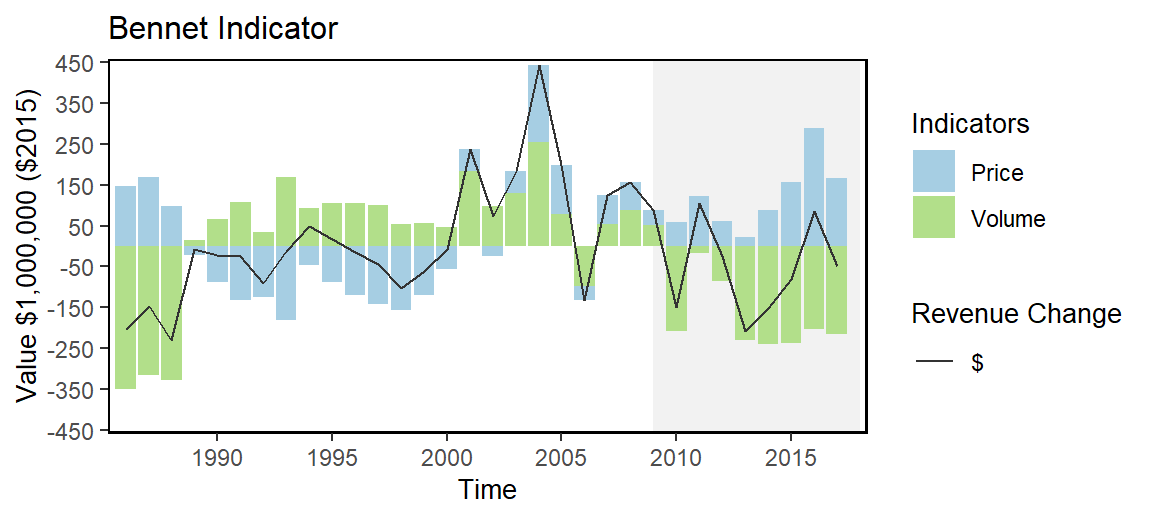
\includegraphics{C:/Users/kimberly.bastille/Desktop/tech-doc/imagesunnamed-chunk-8-1.pdf}
\caption{\label{fig:unnamed-chunk-8}Revenue change from the long-term mean
in 2015 dollars (black), Price (PI), and Volume Indicators (VI) for
commercial landings in the Mid-Atlantic.}
\end{figure}

\chapter{Bottom temperatures}\label{bottom-temperatures}

\textbf{Description}: Time series of annual in situ bottom temperatures
on the Northeast Continental Shelf.

\textbf{Indicator category}: Extensive analysis; not yet published Found
in: State of the Ecosystem - Gulf of Maine \& Georges Bank (2019); State
of the Ecosystem - Mid-Atlantic Bight (2019)

\textbf{Contributor(s)}: Paula Fratantoni,
\href{mailto:paula.fratantoni@noaa.gov}{\nolinkurl{paula.fratantoni@noaa.gov}}

\textbf{Data steward}: Kimberly Bastille,
\href{mailto:kimberly.bastille@noaa.gov}{\nolinkurl{kimberly.bastille@noaa.gov}}

\textbf{Point of contact}: Paula Fratantoni,
\href{mailto:paula.fratantoni@noaa.gov}{\nolinkurl{paula.fratantoni@noaa.gov}}

\textbf{Public availability statement}: Source data are publicly
available at
\url{ftp://ftp.nefsc.noaa.gov/pub/hydro/matlab_files/yearly} and in the
World Ocean Database housed at
\url{http://www.nodc.noaa.gov/OC5/SELECT/dbsearch/dbsearch.html} under
institute code number 258.

\section{Methods}\label{methods-4}

\subsection{Data sources}\label{data-sources-4}

The bottom temperature index incorporates near-bottom temperature
measurements collected on Northeast Fisheries Science Center (NEFSC)
surveys between 1977-present. Early measurements were made using surface
bucket samples, mechanical bathythermographs and expendable
bathythermograph probes, but by 1991 the CTD -- an acronym for
conductivity temperature and depth -- became standard equipment on all
NEFSC surveys. Near-bottom refers to the deepest observation at each
station that falls within 10 m of the reported water depth. Observations
encompass the entire continental shelf area extending from Cape
Hatteras, NC to Nova Scotia, Canada, inclusive of the Gulf of Maine and
Georges Bank.

\subsection{Data extraction}\label{data-extraction-4}

While all processed hydrographic data are archived in an Oracle database
(OCDBS), we work from Matlab-formatted files stored locally.

\subsection{Data analysis}\label{data-analysis-3}

Ocean temperature on the Northeast U.S. Shelf varies significantly on
seasonal timescales. Any attempt to resolve year-to-year changes
requires that this seasonal variability be quantified and removed to
avoid bias. This process is complicated by the fact that NEFSC
hydrographic surveys conform to a random stratified sampling design
meaning that stations are not repeated at fixed locations year after
year so that temperature variability cannot be assessed at fixed station
locations. Instead, we consider the variation of the average bottom
temperature within four \protect\hyperlink{epu}{Ecological Production
Units} (EPUs): Middle Atlantic Bight, Georges Bank, Gulf of Maine and
Scotian Shelf. Within each EPU, ocean temperature observations are
extracted from the collection of measurements made within 10 m of the
bottom on each survey and an area-weighted average temperature is
calculated. The result of this calculation is a timeseries of regional
average near-bottom temperature having a temporal resolution that
matches the survey frequency in the database. Anomalies are subsequently
calculated relative to a reference annual cycle, estimated using a
multiple linear regression model to fit an annual harmonic (365-day
period) to historical regional average temperatures from 1981-2010. The
curve fitting technique to formulate the reference annual cycle follows
the methodologies outlined by Mountain
(\protect\hyperlink{ref-mountain1991}{1991}). The reference period was
chosen because it is the standard climatological period adopted by the
World Meteorological Organization. The resulting anomaly time series
represents the difference between the time series of regional mean
temperatures and corresponding reference temperatures predicted by a
reference annual cycle for the same time of year. Finally, a reference
annual average temperature (calculated as the average across the
reference annual cycle) is added back into the anomaly timeseries to
convert temperature anomalies back to ocean bottom temperature.

\subsection{Data processing}\label{data-processing-2}

Derived bottom temperature data were formatted for inclusion in the
\texttt{ecodata} R package using the following R code.

\begin{Shaded}
\begin{Highlighting}[]
\CommentTok{# Process ocean temperature anomaly data}

\CommentTok{# These data include in situ regional time series of both surface and bottom water temperature anomalies}
\CommentTok{# on the Northeast Continental Shelf. Raw data is split into four files by EPU (SS, GOM, GB, and MAB).}


\KeywordTok{library}\NormalTok{(dplyr)}
\KeywordTok{library}\NormalTok{(tidyr)}
\KeywordTok{library}\NormalTok{(lubridate)}

\CommentTok{#Get raw}
\NormalTok{raw.dir <-}\StringTok{ }\NormalTok{here}\OperatorTok{::}\KeywordTok{here}\NormalTok{(}\StringTok{"data-raw"}\NormalTok{) }\CommentTok{#input raw}

\NormalTok{get_oceantemp_insitu <-}\StringTok{ }\ControlFlowTok{function}\NormalTok{(}\DataTypeTok{save_clean =}\NormalTok{ F)\{}

\NormalTok{  ss <-}\StringTok{ }\KeywordTok{read.csv}\NormalTok{(}\KeywordTok{file.path}\NormalTok{(raw.dir,}\StringTok{"EcoSS_core_Ttopbot.csv"}\NormalTok{)) }\OperatorTok\StringTok{ }\KeywordTok{mutate}\NormalTok{(}\DataTypeTok{EPU =} \StringTok{"SS"}\NormalTok{)}
\NormalTok{  gom <-}\StringTok{ }\KeywordTok{read.csv}\NormalTok{(}\KeywordTok{file.path}\NormalTok{(raw.dir,}\StringTok{"EcoGoM_core_Ttopbot.csv"}\NormalTok{)) }\OperatorTok\StringTok{ }\KeywordTok{mutate}\NormalTok{(}\DataTypeTok{EPU =} \StringTok{"GOM"}\NormalTok{)}
\NormalTok{  gb <-}\StringTok{ }\KeywordTok{read.csv}\NormalTok{(}\KeywordTok{file.path}\NormalTok{(raw.dir,}\StringTok{"EcoGB_core_Ttopbot.csv"}\NormalTok{)) }\OperatorTok\StringTok{ }\KeywordTok{mutate}\NormalTok{(}\DataTypeTok{EPU =} \StringTok{"GB"}\NormalTok{)}
\NormalTok{  mab <-}\StringTok{ }\KeywordTok{read.csv}\NormalTok{(}\KeywordTok{file.path}\NormalTok{(raw.dir,}\StringTok{"EcoMAB_core_Ttopbot.csv"}\NormalTok{)) }\OperatorTok\StringTok{ }\KeywordTok{mutate}\NormalTok{(}\DataTypeTok{EPU =} \StringTok{"MAB"}\NormalTok{)}
  
\NormalTok{  oceantemp_insitu <-}\StringTok{ }\KeywordTok{rbind}\NormalTok{(ss, gom, gb, mab) }\OperatorTok\StringTok{ }\CommentTok{#bind all}
\StringTok{    }\NormalTok{dplyr}\OperatorTok{::}\KeywordTok{rename}\NormalTok{(}\DataTypeTok{Time =}\NormalTok{ decimal.year, }\DataTypeTok{Var =}\NormalTok{ variable.name, }\DataTypeTok{Value =}\NormalTok{ temperature) }\OperatorTok\StringTok{ }\CommentTok{#rename}
\StringTok{    }\KeywordTok{mutate}\NormalTok{(}\DataTypeTok{Units =} \StringTok{"degreesC"}\NormalTok{, }\DataTypeTok{Time =} \KeywordTok{as.Date}\NormalTok{(}\KeywordTok{format}\NormalTok{(}\KeywordTok{date_decimal}\NormalTok{(Time), }\StringTok{"%Y-%b-%d"}\NormalTok{), }\StringTok{"%Y-%b-%d"}\NormalTok{),}
\NormalTok{           Var, }\DataTypeTok{Var =}\NormalTok{ plyr}\OperatorTok{::}\KeywordTok{mapvalues}\NormalTok{(Var, }\DataTypeTok{from =} \KeywordTok{c}\NormalTok{(}\StringTok{"Tsfc_anom"}\NormalTok{,}\CommentTok{#Rename variables}
                                                    \StringTok{"Tsfc_ref"}\NormalTok{,}
                                                    \StringTok{"Tbot_anom"}\NormalTok{,}
                                                    \StringTok{"Tbot_ref"}\NormalTok{),}
                                      \DataTypeTok{to =} \KeywordTok{c}\NormalTok{(}\StringTok{"sst anomaly in situ"}\NormalTok{,}
                                             \StringTok{"reference sst in situ (1981-2010)"}\NormalTok{,}
                                             \StringTok{"bottom temp anomaly in situ"}\NormalTok{,}
                                             \StringTok{"reference bt in situ (1981-2010)"}\NormalTok{))) }\OperatorTok\StringTok{ }
\StringTok{    }\KeywordTok{group_by}\NormalTok{(}\DataTypeTok{Time =} \KeywordTok{year}\NormalTok{(Time), EPU, Var, Units) }\OperatorTok
\StringTok{    }\NormalTok{dplyr}\OperatorTok{::}\KeywordTok{summarise}\NormalTok{(}\DataTypeTok{Value =} \KeywordTok{mean}\NormalTok{(Value)) }\OperatorTok
\StringTok{    }\KeywordTok{as.data.frame}\NormalTok{() }
  
  \ControlFlowTok{if}\NormalTok{ (save_clean)\{}
\NormalTok{    usethis}\OperatorTok{::}\KeywordTok{use_data}\NormalTok{(oceantemp_insitu, }\DataTypeTok{overwrite =}\NormalTok{ T)}
\NormalTok{  \} }\ControlFlowTok{else}\NormalTok{ \{}
    \KeywordTok{return}\NormalTok{(oceantemp_insitu)}
\NormalTok{  \}}
\NormalTok{\}}
\end{Highlighting}
\end{Shaded}

\subsection{Plotting}\label{plotting-3}

\begin{Shaded}
\begin{Highlighting}[]
\NormalTok{bot_temp_insitu_gom <-}\StringTok{ }\NormalTok{oceantemp_insitu }\OperatorTok
\StringTok{  }\KeywordTok{filter}\NormalTok{(EPU }\OperatorTok{==}\StringTok{ "GOM"}\NormalTok{,}
\NormalTok{         Var }\OperatorTok{==}\StringTok{ "bottom temp anomaly in situ"}\NormalTok{) }\OperatorTok\StringTok{ }
\StringTok{  }\KeywordTok{mutate}\NormalTok{(}\DataTypeTok{hline =} \DecValTok{0}\NormalTok{) }\OperatorTok\StringTok{ }
\StringTok{    }\KeywordTok{ggplot}\NormalTok{()}\OperatorTok{+}\StringTok{ }\CommentTok{#plot}
\StringTok{     }\KeywordTok{annotate}\NormalTok{(}\StringTok{"rect"}\NormalTok{, }\DataTypeTok{fill =}\NormalTok{ shade.fill, }\DataTypeTok{alpha =}\NormalTok{ shade.alpha,}
      \DataTypeTok{xmin =}\NormalTok{ x.shade.min , }\DataTypeTok{xmax =}\NormalTok{ x.shade.max,}
      \DataTypeTok{ymin =} \OperatorTok{-}\OtherTok{Inf}\NormalTok{, }\DataTypeTok{ymax =} \OtherTok{Inf}\NormalTok{) }\OperatorTok{+}
\StringTok{  }\KeywordTok{geom_line}\NormalTok{(}\KeywordTok{aes}\NormalTok{(}\DataTypeTok{x =}\NormalTok{ Time, }\DataTypeTok{y =}\NormalTok{ Value)) }\OperatorTok{+}
\StringTok{  }\KeywordTok{geom_gls}\NormalTok{(}\KeywordTok{aes}\NormalTok{(}\DataTypeTok{x =}\NormalTok{ Time, }\DataTypeTok{y =}\NormalTok{ Value)) }\OperatorTok{+}
\StringTok{  }\KeywordTok{geom_point}\NormalTok{(}\KeywordTok{aes}\NormalTok{(}\DataTypeTok{x =}\NormalTok{ Time, }\DataTypeTok{y =}\NormalTok{ Value), }\DataTypeTok{size =} \DecValTok{1}\NormalTok{) }\OperatorTok{+}
\StringTok{  }\KeywordTok{ylab}\NormalTok{(}\StringTok{"Temp. Anomaly (°C)"}\NormalTok{) }\OperatorTok{+}
\StringTok{  }\KeywordTok{ggtitle}\NormalTok{(}\StringTok{"GOM Bottom Temperature Anomaly"}\NormalTok{) }\OperatorTok{+}
\StringTok{  }\KeywordTok{scale_x_continuous}\NormalTok{(}\DataTypeTok{expand =} \KeywordTok{c}\NormalTok{(}\FloatTok{0.01}\NormalTok{, }\FloatTok{0.01}\NormalTok{)) }\OperatorTok{+}
\StringTok{    }\KeywordTok{geom_hline}\NormalTok{(}\KeywordTok{aes}\NormalTok{(}\DataTypeTok{yintercept =}\NormalTok{ hline),}
           \DataTypeTok{size =}\NormalTok{ hline.size,}
           \DataTypeTok{alpha =}\NormalTok{ hline.alpha,}
           \DataTypeTok{linetype =}\NormalTok{ hline.lty) }\OperatorTok{+}
\StringTok{  }\KeywordTok{theme_ts}\NormalTok{() }\OperatorTok{+}
\StringTok{  }\KeywordTok{theme}\NormalTok{(}\DataTypeTok{strip.text=}\KeywordTok{element_text}\NormalTok{(}\DataTypeTok{hjust=}\DecValTok{0}\NormalTok{),}
        \DataTypeTok{plot.title =} \KeywordTok{element_text}\NormalTok{(}\DataTypeTok{size =} \DecValTok{12}\NormalTok{))}


\NormalTok{bot_temp_insitu_gb <-}\StringTok{ }\NormalTok{oceantemp_insitu }\OperatorTok
\StringTok{  }\KeywordTok{filter}\NormalTok{(EPU }\OperatorTok{==}\StringTok{ "GB"}\NormalTok{,}
\NormalTok{         Var }\OperatorTok{==}\StringTok{ "bottom temp anomaly in situ"}\NormalTok{) }\OperatorTok
\StringTok{   }\KeywordTok{mutate}\NormalTok{(}\DataTypeTok{hline =} \DecValTok{0}\NormalTok{) }\OperatorTok\StringTok{ }
\StringTok{    }\KeywordTok{ggplot}\NormalTok{()}\OperatorTok{+}\StringTok{ }\CommentTok{#plot}
\StringTok{     }\KeywordTok{annotate}\NormalTok{(}\StringTok{"rect"}\NormalTok{, }\DataTypeTok{fill =}\NormalTok{ shade.fill, }\DataTypeTok{alpha =}\NormalTok{ shade.alpha,}
      \DataTypeTok{xmin =}\NormalTok{ x.shade.min , }\DataTypeTok{xmax =}\NormalTok{ x.shade.max,}
      \DataTypeTok{ymin =} \OperatorTok{-}\OtherTok{Inf}\NormalTok{, }\DataTypeTok{ymax =} \OtherTok{Inf}\NormalTok{) }\OperatorTok{+}
\StringTok{  }\KeywordTok{geom_line}\NormalTok{(}\KeywordTok{aes}\NormalTok{(}\DataTypeTok{x =}\NormalTok{ Time, }\DataTypeTok{y =}\NormalTok{ Value)) }\OperatorTok{+}
\StringTok{  }\KeywordTok{geom_gls}\NormalTok{(}\KeywordTok{aes}\NormalTok{(}\DataTypeTok{x =}\NormalTok{ Time, }\DataTypeTok{y =}\NormalTok{ Value)) }\OperatorTok{+}
\StringTok{  }\KeywordTok{geom_point}\NormalTok{(}\KeywordTok{aes}\NormalTok{(}\DataTypeTok{x =}\NormalTok{ Time, }\DataTypeTok{y =}\NormalTok{ Value), }\DataTypeTok{size =} \DecValTok{1}\NormalTok{) }\OperatorTok{+}
\StringTok{  }\KeywordTok{ylab}\NormalTok{(}\StringTok{"Temp. Anomaly (°C)"}\NormalTok{) }\OperatorTok{+}
\StringTok{  }\KeywordTok{ggtitle}\NormalTok{(}\StringTok{"GB Bottom Temperature Anomaly"}\NormalTok{) }\OperatorTok{+}
\StringTok{  }\KeywordTok{scale_x_continuous}\NormalTok{(}\DataTypeTok{expand =} \KeywordTok{c}\NormalTok{(}\FloatTok{0.01}\NormalTok{, }\FloatTok{0.01}\NormalTok{)) }\OperatorTok{+}
\StringTok{    }\KeywordTok{geom_hline}\NormalTok{(}\KeywordTok{aes}\NormalTok{(}\DataTypeTok{yintercept =}\NormalTok{ hline),}
           \DataTypeTok{size =}\NormalTok{ hline.size,}
           \DataTypeTok{alpha =}\NormalTok{ hline.alpha,}
           \DataTypeTok{linetype =}\NormalTok{ hline.lty) }\OperatorTok{+}
\StringTok{  }\KeywordTok{theme_ts}\NormalTok{() }\OperatorTok{+}
\StringTok{  }\KeywordTok{theme}\NormalTok{(}\DataTypeTok{strip.text=}\KeywordTok{element_text}\NormalTok{(}\DataTypeTok{hjust=}\DecValTok{0}\NormalTok{),}
        \DataTypeTok{plot.title =} \KeywordTok{element_text}\NormalTok{(}\DataTypeTok{size =} \DecValTok{12}\NormalTok{))}



\NormalTok{bot_temp_insitu_gom }\OperatorTok{+}
\StringTok{ }\NormalTok{bot_temp_insitu_gb }\OperatorTok{+}\StringTok{ }\KeywordTok{plot_layout}\NormalTok{(}\DataTypeTok{nrow =} \DecValTok{1}\NormalTok{)}
\end{Highlighting}
\end{Shaded}

\begin{figure}

{\centering 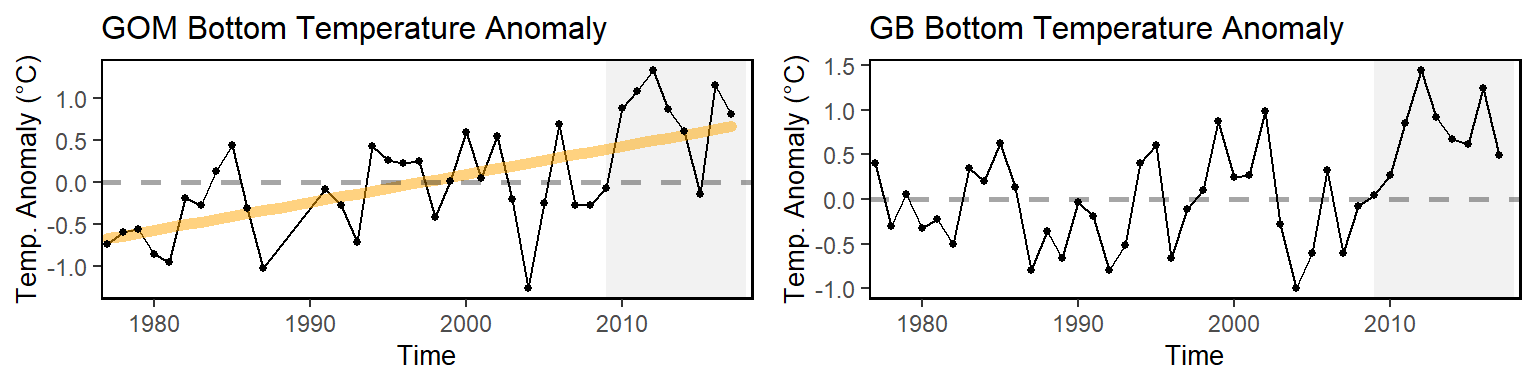
\includegraphics{C:/Users/kimberly.bastille/Desktop/tech-doc/imagesunnamed-chunk-10-1} 

}

\caption{GOM and GB annual bottom temperature anomalies.}\label{fig:unnamed-chunk-10}
\end{figure}

\begin{Shaded}
\begin{Highlighting}[]
  \CommentTok{#plot_layout(ncol =  1) &}
  \CommentTok{#theme(plot.margin = unit(c(0, 0, 0, 0), "cm"))}
\end{Highlighting}
\end{Shaded}

\chapter{Catch and Fleet Diversity}\label{catch-and-fleet-diversity}

\textbf{Description}: Permit-level species diversity and Council-level
fleet diversity.

\textbf{Found in}: State of the Ecosystem - Gulf of Maine \& Georges
Bank (2018), State of the Ecosystem - Mid-Atlantic (2018)

\textbf{Indicator category}: Database pull with analysis; Published
methods

\textbf{Contributor(s)}: Geret DePiper, Min-Yang Lee

\textbf{Data steward}: Geret DePiper,
\href{mailto:geret.depiper@noaa.gov}{\nolinkurl{geret.depiper@noaa.gov}}

\textbf{Point of contact}: Geret DePiper,
\href{mailto:geret.depiper@noaa.gov}{\nolinkurl{geret.depiper@noaa.gov}}

\textbf{Public availability statement}: Source data is not publicly
availabe due to PII restrictions. Derived time series are available for
download
\href{https://comet.nefsc.noaa.gov/erddap/tabledap/comm_data_soe_v1.html}{here}.

\section{Methods}\label{methods-5}

Diversity estimates have been developed to understand whether
specialization, or alternatively stovepiping, is occurring in fisheries
of the Northeastern Large Marine Ecosystem. We use the average effective
Shannon indices for species revenue at the permit level, for all permits
landing any amount of \href{https://www.nefmc.org/}{NEFMC} or
\href{http://www.mafmc.org/}{MAFMC} Fishery Management Plan (FMP)
species within a year (including both Monkfish and Spiny Dogfish). We
also use the effective Shannon index of fleet revenue diversity and
count of active fleets to assess the extent to which the distribution of
fishing changes across fleet segments.

\subsection{Data sources}\label{data-sources-5}

Data for these diversity estimates comes from a variety of sources,
including the Commercial Fishery Dealer Database, Vessel Trip Reports,
Clam logbooks, vessel characteristics from Permit database, WPU series
producer price index. These data are typically not available to the
public.

\subsection{Data extraction}\label{data-extraction-5}

The following describes both the permit-level species and fleet
diversity data generation. Price data was extracted from the Commercial
Fishery Dealer database (CFDERS) and linked to Vessel Trip Reports by a
heirarchical matching algorithm that matched date and port of landing at
its highest resolution. Code used in these analyses is available upon
request.

Output data was then matched to vessel characteristics from the VPS
VESSEL data set. For the permit-level estimate, species groups are based
off of a slightly refined NESPP3 code, defined in the data as ``myspp'',
which is further developed in the script to rectify inconsistencies in
the data.

Species groups used include Highly Migratory Species, Monkfish, Atlantic
Sea Scallops, Shrimp, Skates, Atlantic Herring, Ocean Quahog, Surf Clam,
Tilefish, Black Sea Bass and Fluke, Butterfish and Red Hake and Unknown
Whiting, Bluefish, Spiny Dogfish, Illex, American Lobster, Loligo,
Menhaden, Offshore hake, Scup, Sand Dabs, Pout, Wolffish, Winter
Flounder, Yellowtail Flounder, Unspecified hakes, White hake, Halibut,
Bluefish \& Scup (NE only), New England Groundfish (cod, pollock,
hadddock, Monkfish, Winter flounder, Witch flounder, White hake, Plaice,
redfish), Mid-Atlantic Groundfish (cod, wolffish, plaice, Witch
flounder, haddock, pollock, redfish, and halibut), pout and windowpane
flounder (MA only), and an ``Other'' category for all other species.

For the fleet diversity metric, gears include scallop dredge (gearcodes
DRS, DSC, DTC, and DTS), other dredges (gearcodes DRM, DRO, and DRU),
gillnet (gearcodes GND, GNT, GNO, GNR, and GNS), hand (gearcode HND),
longline (gearcodes LLB and LLP), bottom trawl (gearcodes OTB, OTF, OTO,
OTC. OTS, OHS, OTR, OTT, and PTB), midwater trawls (gearcode OTM and
PTM), pot (gearcodes PTL, PTW, PTC, PTE, PTF, PTH, PTL, PTO, PTS, and
PTX), purse seine (gearcode PUR), and hydraulic clam dredge (gearcode
DRC).Vessels were further grouped by length categories of less than 30
feet, 30 to 50 feet, 50 to 75 feet, and 75 feet and above. All revenue
was deflated to real dollars using the ``WPU0223'' Producer Price Index
with a base of January 2015. Stata code for data processing is available
\href{https://github.com/NOAA-EDAB/tech-doc/tree/master/data/Human_Dimensions_code}{here}.

\subsection{Data analysis}\label{data-analysis-4}

This permit-level species effective Shannon index is calculated as
\[exp(-\sum_{i=1}^{N}p_{ijt}ln(p_{ijt}))\] for all \(j\), with
\(p_{ijt}\) representing the proportion of revenue generated by species
or species group \(i\) for permit \(j\) in year \(t\), and is a
composite of richness (the number of species landed) and abundance (the
revenue generated from each species). The annual arithmetic mean value
of the effective Shannon index across permits is used as the indicator
of permit-level species diversity.

In a similar manner, the fleet diversity metric is estimated as
\[exp(-\sum_{i=1}^{N}p_{kt}ln(p_{kt})) \] for all \(k\), where
\(p_{kt}\) represents the proportion of total revenue generated by fleet
segment \(k\) (gear and length combination) per year \(t\). The indices
each run from 1996 to 2017. A count of the number of fleets active in
every year is also provided to assess whether changes in fleet diversity
are caused by shifts in abundance (number of fleets), or evenness
(concentration of revenue). The work is based off of analysis conducted
in Thunberg and Correia
(\protect\hyperlink{ref-eric_m_thunberg_measures_2015}{2015}) and
published in Gaichas et al.
(\protect\hyperlink{ref-gaichas_framework_2016}{2016}).

\subsection{Data processing}\label{data-processing-3}

Catch and fleet diversity indicators were formatted for inclusion in the
\texttt{ecodata} R package using the following R script.

\begin{Shaded}
\begin{Highlighting}[]
\CommentTok{# Process commercial diversity data}

\CommentTok{# More information about these data are available at https://noaa-edab.github.io/tech-doc/catch-and-fleet-diversity.html.}
\CommentTok{# Data are drawn from blend of VTR trip data, CFDBS prices, vessel characteristics from PERMIT databases, }
\CommentTok{# and major VTR gear by permit. Here "MA" and "NE" refer to the Mid-Atlantic and New England regions respectively, and are }
\CommentTok{# not derived by EPU.}

\KeywordTok{library}\NormalTok{(dplyr)}
\KeywordTok{library}\NormalTok{(tidyr)}
\KeywordTok{library}\NormalTok{(stringr)}

\NormalTok{raw.dir <-}\StringTok{ }\NormalTok{here}\OperatorTok{::}\KeywordTok{here}\NormalTok{(}\StringTok{"data-raw"}\NormalTok{)}

\NormalTok{get_commercial_div <-}\StringTok{ }\ControlFlowTok{function}\NormalTok{(}\DataTypeTok{save_clean =}\NormalTok{ F)\{}
\NormalTok{  commercial_div <-}\StringTok{ }\KeywordTok{read.csv}\NormalTok{(}\KeywordTok{file.path}\NormalTok{(raw.dir, }\StringTok{"Commercial_Diversity_2018.csv"}\NormalTok{)) }\OperatorTok
\StringTok{    }\NormalTok{dplyr}\OperatorTok{::}\KeywordTok{select}\NormalTok{(}\OperatorTok{-}\NormalTok{X, }\OperatorTok{-}\NormalTok{Source) }\OperatorTok
\StringTok{    }\NormalTok{dplyr}\OperatorTok{::}\KeywordTok{rename}\NormalTok{(}\DataTypeTok{EPU =}\NormalTok{ Region) }\OperatorTok
\StringTok{    }\KeywordTok{as.data.frame}\NormalTok{()}
  
\NormalTok{  commercial_div}\OperatorTok{$}\NormalTok{Var <-}\StringTok{ }\KeywordTok{str_replace}\NormalTok{(commercial_div}\OperatorTok{$}\NormalTok{Var, }\StringTok{"diveristy"}\NormalTok{, }\StringTok{"diversity"}\NormalTok{)}
  
  \ControlFlowTok{if}\NormalTok{(save_clean)\{}
\NormalTok{    usethis}\OperatorTok{::}\KeywordTok{use_data}\NormalTok{(commercial_div, }\DataTypeTok{overwrite =}\NormalTok{ T)}
\NormalTok{  \} }\ControlFlowTok{else}\NormalTok{ \{}
    \KeywordTok{return}\NormalTok{(commercial_div)}
\NormalTok{  \}}
  
  
\NormalTok{\}}
\end{Highlighting}
\end{Shaded}

\subsection{Plotting}\label{plotting-4}

\begin{Shaded}
\begin{Highlighting}[]
\CommentTok{# Relative working directories}
\NormalTok{data.dir  <-}\StringTok{ }\NormalTok{here}\OperatorTok{::}\KeywordTok{here}\NormalTok{(}\StringTok{'data'}\NormalTok{)}
\NormalTok{r.dir <-}\StringTok{ }\NormalTok{here}\OperatorTok{::}\KeywordTok{here}\NormalTok{(}\StringTok{'R'}\NormalTok{)}

\CommentTok{# Load data}
\KeywordTok{load}\NormalTok{(}\KeywordTok{file.path}\NormalTok{(data.dir,}\StringTok{"SOE_data_erddap.Rdata"}\NormalTok{))}

\CommentTok{# Source plotting functions}
\KeywordTok{source}\NormalTok{(}\KeywordTok{file.path}\NormalTok{(r.dir,}\StringTok{"BasePlot_source.R"}\NormalTok{))}

\NormalTok{opar <-}\StringTok{ }\KeywordTok{par}\NormalTok{(}\DataTypeTok{mfrow =} \KeywordTok{c}\NormalTok{(}\DecValTok{2}\NormalTok{, }\DecValTok{1}\NormalTok{), }\DataTypeTok{mar =} \KeywordTok{c}\NormalTok{(}\DecValTok{0}\NormalTok{, }\DecValTok{0}\NormalTok{, }\DecValTok{0}\NormalTok{, }\DecValTok{0}\NormalTok{), }\DataTypeTok{oma =} \KeywordTok{c}\NormalTok{(}\DecValTok{4}\NormalTok{, }\DecValTok{6}\NormalTok{, }\DecValTok{2}\NormalTok{, }\DecValTok{6}\NormalTok{))}

\KeywordTok{soe.plot}\NormalTok{(SOE.data, }\StringTok{"Time"}\NormalTok{, }\StringTok{"Mid-Atlantic average fleet diversity"}\NormalTok{, }\DataTypeTok{stacked =} \StringTok{"A"}\NormalTok{,}
         \DataTypeTok{rel.y.num =} \FloatTok{0.9}\NormalTok{, }\DataTypeTok{end.start =} \DecValTok{2008}\NormalTok{, }\DataTypeTok{tol =} \FloatTok{0.15}\NormalTok{, }\DataTypeTok{full.trend =}\NormalTok{ F, }\DataTypeTok{cex.stacked =} \FloatTok{1.5}\NormalTok{)}
\KeywordTok{soe.stacked.axis}\NormalTok{(}\StringTok{'Year'}\NormalTok{, }\StringTok{'Fleet diversity'}\NormalTok{, }\DataTypeTok{y.line =} \FloatTok{2.5}\NormalTok{, }\DataTypeTok{outer =}\NormalTok{ F,}
                 \DataTypeTok{rel.x.text =} \DecValTok{1}\NormalTok{, }\DataTypeTok{rel.y.text =} \DecValTok{1}\NormalTok{)}
\KeywordTok{soe.plot}\NormalTok{(SOE.data,}\StringTok{"Time"}\NormalTok{, }\StringTok{"Mid-Atlantic fleet count"}\NormalTok{, }\DataTypeTok{stacked =} \StringTok{"B"}\NormalTok{,}
         \DataTypeTok{rel.y.num =} \FloatTok{0.9}\NormalTok{, }\DataTypeTok{end.start =} \DecValTok{2008}\NormalTok{, }\DataTypeTok{full.trend =}\NormalTok{ F, }\DataTypeTok{cex.stacked =} \FloatTok{1.5}\NormalTok{)}

\KeywordTok{soe.stacked.axis}\NormalTok{(}\StringTok{'Year'}\NormalTok{, }\StringTok{'Fleet count'}\NormalTok{, }\DataTypeTok{y.line =} \FloatTok{2.5}\NormalTok{, }\DataTypeTok{outer =}\NormalTok{ F,}
                 \DataTypeTok{rel.x.text =} \DecValTok{1}\NormalTok{, }\DataTypeTok{rel.y.text =} \FloatTok{0.95}\NormalTok{)}
\end{Highlighting}
\end{Shaded}

\begin{figure}

{\centering 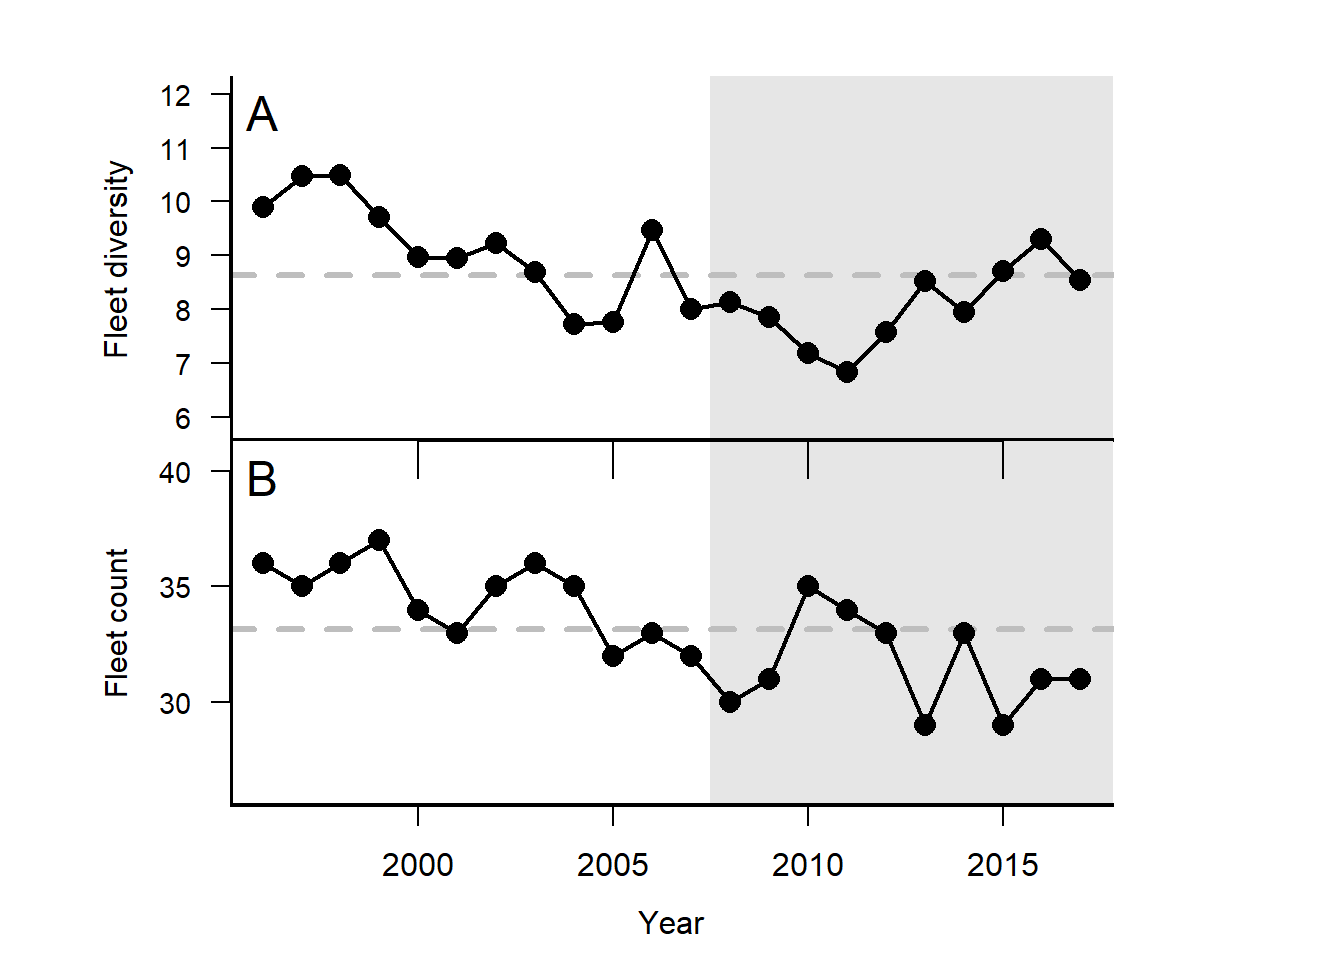
\includegraphics{C:/Users/kimberly.bastille/Desktop/tech-doc/imagesfleet-diversity-1} 

}

\caption{Fleet diversity (A) and fleet count (B) in the Mid Atlantic Bight.}\label{fig:fleet-diversity}
\end{figure}

\chapter{Chesapeake Bay Water Quality Standards
Attainment}\label{chesapeake-bay-water-quality-standards-attainment}

\textbf{Description}: A multimetric indicator describing the attainment
status of Chesapeake Bay with respect to three water quality standards
criteria, namely, dissolved oxygen, chlorophyll-a, and water
clarity/submerged aquatic vegetation.

\textbf{Indicator category}: Published method; Database pull with
analysis

\textbf{Found in}: State of the Ecosystem - Mid-Atlantic (2019)

\textbf{Contributor(s)}: Qian Zhang, Rebecca Murphy, Richard Tian,
Melinda Forsyth, Emily Trentacoste, Jeni Keisman, and Peter Tango.

\textbf{Data steward}: Qian Zhang,
\href{mailto:qzhang@chesapeakebay.net}{\nolinkurl{qzhang@chesapeakebay.net}}

\textbf{Point of contact}: Qian Zhang,
\href{mailto:qzhang@chesapeakebay.net}{\nolinkurl{qzhang@chesapeakebay.net}}

\textbf{Public availability statement}: Data are publicly available (see
Data Sources below).

\section{Methods}\label{methods-6}

To protect the aquatic living resources of Chesapeake Bay, the
\href{https://www.chesapeakebay.net/}{Chesapeake Bay Program} (CBP)
partnership has developed a guidance framework of ambient water quality
criteria with designated uses and assessment procedures for dissolved
oxygen, chlorophyll-a, and water clarity/submerged aquatic vegetation
(SAV) (USEPA \protect\hyperlink{ref-usepa2003}{2003}). To achieve
consistent assessment over time and between jurisdictions, a multimetric
indicator was proposed by the CBP partnership to provide a means for
tracking the progress in all 92 management segments of Chesapeake Bay
(USEPA \protect\hyperlink{ref-usepa2017}{2017}). This indicator has been
computed for each three-year assessment period since 1985-1987,
providing an integrated measure of Chesapeake Bay's water quality
condition over the last three decades.

\subsection{Data sources}\label{data-sources-6}

The multimetric indicator required monitoring data on dissolved oxygen
(DO) concentrations, chlorophyll-a concentrations, water clarity, SAV
acreage, water temperature, and salinity. SAV acreage has been measured
by the Virginia Institute of Marine Science in collaboration with the
CBP, which is available via
\url{http://web.vims.edu/bio/sav/StateSegmentAreaTable.htm}. Data for
all other parameters were obtained from the
\href{http://www.chesapeakebay.net/data/downloads/cbp_water_quality_database_1984_present}{CBP
Water Quality Database}. These data have been routinely reported to the
CBP by the Maryland Department of Natural Resources, Virginia Department
of Environmental Quality, Old Dominion University, Virginia Institute of
Marine Science, and citizen/volunteer monitoring initiatives.

\subsection{Data analysis}\label{data-analysis-5}

\textbf{Criteria attainment assessment}

Monitoring data of DO, chlorophyll-a, and water clarity/SAV were
processed and compared with water quality criteria thresholds according
to different designated uses (DUs). These DUs are migratory spawning and
nursery (MSN), open water (OW), deep water (DW), deep channel (DC), and
shallow water (SW), which reflect the seasonal nature of water column
structure and the life history needs of living resources. Station-level
DO and chlorophyll-a data were spatially interpolated in three
dimensions.

Salinity and water temperature data were used to compute the vertical
density structure of the water column, which was translated into layers
of different DUs. Criteria attainment was determined by comparing
violation rates over a 3-year period to a reference cumulative frequency
distribution that represents the extent of allowable violation. This
approach was implemented using FORTRAN codes, which are provided as a
zipped folder. For water clarity/SAV, the single best year in the 3-year
assessment period was compared with the segment-specific acreage goal,
the water clarity goal, or a combination of both. For more details,
refer to the Methods section of Zhang et al.
(\protect\hyperlink{ref-zhang2018}{2018}).

\textbf{Indicator calculation}

The multimetric indicator quantifies the fraction of
segment-DU-criterion combinations that meet all applicable
season-specific thresholds for each 3-year assessment period from
1985-1987 to 2015-2017. For each 3-year assessment period, all
applicable segment-DU-criterion combinations were evaluated in a
binomial fashion and scored 1 for ``in attainment'' and 0 for
``nonattainment''. The classified status of each segment-DU-criterion
combination was weighted via segments' surface area and summed to obtain
the multimetric index score. This weighting scheme was adopted for two
reasons: (1) segments vary in size over four orders of magnitude, and
(2) surface area of each segment does not change with time or DUs,
unlike seasonally variable habitat volume or bottom water area (USEPA
\protect\hyperlink{ref-usepa2017}{2017}). For more details, refer to the
Methods section of Zhang et al.
(\protect\hyperlink{ref-zhang2018}{2018}).

The indicator provides an integrated measure of Chesapeake Bay's water
quality condition (Figure 1). In 2015-2017, 42\% of all tidal water
segment-DU-criterion combinations are estimated to have met or exceeded
applicable water quality criteria thresholds, which marks the best
3-year status since 1985-1987. The indicator has a positive and
statistically significant trend from 1985 to 2017, which shows that
Chesapeake Bay is on a positive trajectory toward recovery. This pattern
was statistically linked to total nitrogen reduction, indicating
responsiveness of attainment status to management actions implemented to
reduce nutrients in the system.

\begin{figure}
\centering
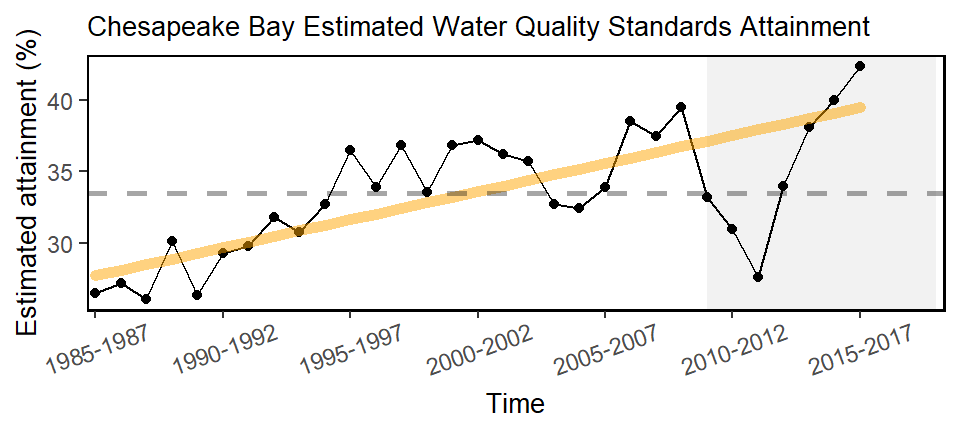
\includegraphics{C:/Users/kimberly.bastille/Desktop/tech-doc/imagesunnamed-chunk-12-1.pdf}
\caption{\label{fig:unnamed-chunk-12}Time series of the multimetric
indicator score for estimated Chesapeake Bay water quality standards
attainment for each 3-year assessment period between 1985-1987 and
2015-2017. A significant positive trend for the time series is shown by
the orange line (p \textless{} 0.05).}
\end{figure}

Patterns of attainment of individual DUs are variable (Figure 2).
Changes in OW-DO, DC-DO, and water clarity/SAV have shown long-term
improvements, which have contributed to overall attainment indicator
improvement. By contrast, the MSN-DO attainment experienced a sharp
spike in the first few assessment periods but generally degraded after
the 1997-1999, which has implications to the survival, growth, and
reproduction of the migratory and resident tidal freshwater fish during
spawning and nursery season in the tidal freshwater to low-salinity
habitats. The status and trends of tidal segments' attainment may be
used to inform siting decisions of aquaculture operations in Chesapeake
Bay.

\begin{figure}
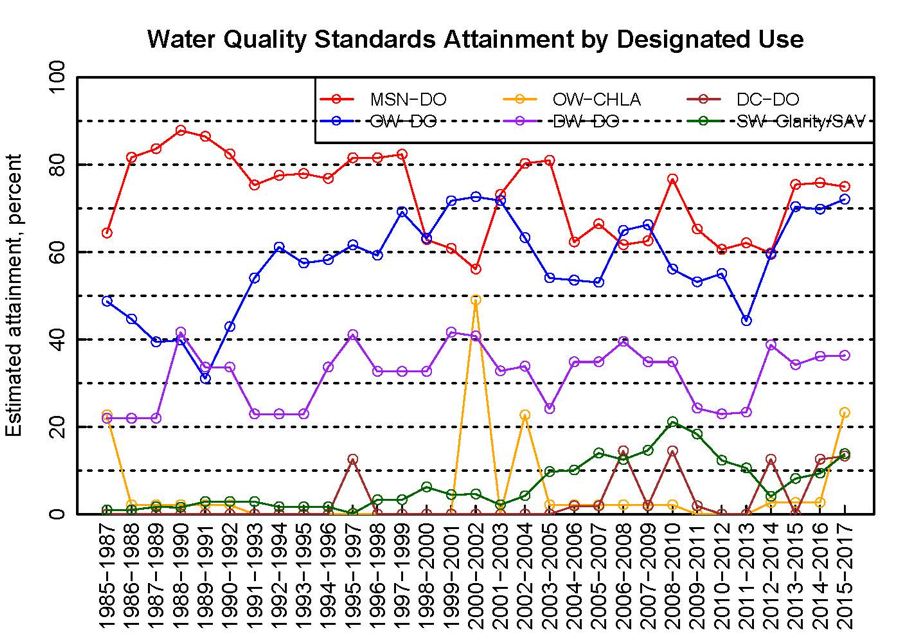
\includegraphics[width=12.49in]{C:/Users/kimberly.bastille/Desktop/tech-doc/images/cb_water_quality_attainment} \caption{Time series of the estimated attainment of water quality standards (i.e., DO: dissolved oxygen; CHLA: chlorophyll-a; Clarity/SAV: water clarity/submerged aquatic vegetation) for five Chesapeake Bay designated uses (MSN: migratory spawning and nursery; OW: open water; DW: deep water; DC: deep channel; SW: shallow water) for each 3-year assessment period between 1985-1987 and 2015-2017.}\label{fig:unnamed-chunk-13}
\end{figure}

\subsection{Data processing}\label{data-processing-4}

The indicator data set was formatted for inclusion in the ecodata R
package using the following R script.

\begin{Shaded}
\begin{Highlighting}[]
\CommentTok{#Chesapeake bay water quality attainment indicator}

\KeywordTok{library}\NormalTok{(dplyr)}
\KeywordTok{library}\NormalTok{(tidyr)}


\NormalTok{raw.dir <-}\StringTok{ }\NormalTok{here}\OperatorTok{::}\KeywordTok{here}\NormalTok{(}\StringTok{"data-raw"}\NormalTok{)}

\NormalTok{get_ches_bay_wq <-}\StringTok{ }\ControlFlowTok{function}\NormalTok{(}\DataTypeTok{save_clean =}\NormalTok{F)\{}
\NormalTok{  ches_bay_wq <-}\StringTok{ }\KeywordTok{read.csv}\NormalTok{(}\KeywordTok{file.path}\NormalTok{(raw.dir, }\StringTok{"Attainment_indicator.csv"}\NormalTok{)) }\OperatorTok\StringTok{ }
\StringTok{    }\NormalTok{dplyr}\OperatorTok{::}\KeywordTok{select}\NormalTok{(}\DataTypeTok{Time =}\NormalTok{ Year.}\DecValTok{1}\NormalTok{, }\DataTypeTok{Value =}\NormalTok{ Total) }\OperatorTok\StringTok{ }
\StringTok{    }\KeywordTok{mutate}\NormalTok{(}\DataTypeTok{Var =} \StringTok{"chesapeake bay water quality attainment"}\NormalTok{,}
           \DataTypeTok{Units =} \StringTok{"estimated attainment, percent"}\NormalTok{,}
           \DataTypeTok{EPU =} \StringTok{"MAB"}\NormalTok{)}
  
  \ControlFlowTok{if}\NormalTok{ (save_clean)\{}
\NormalTok{    usethis}\OperatorTok{::}\KeywordTok{use_data}\NormalTok{(ches_bay_wq, }\DataTypeTok{overwrite =}\NormalTok{ T)}
\NormalTok{  \} }\ControlFlowTok{else}\NormalTok{ \{}
    \KeywordTok{return}\NormalTok{(ches_bay_wq)}
\NormalTok{  \}}
\NormalTok{\}}
\end{Highlighting}
\end{Shaded}

\hypertarget{chl-pp}{\chapter{\texorpdfstring{Chlorophyll \emph{a} and
Primary
Production}{Chlorophyll a and Primary Production}}\label{chl-pp}}

\textbf{Description}: Chlorophyll \emph{a} and Primary Production

\textbf{Found in}: State of the Ecosystem - Gulf of Maine \& Georges
Bank (2018, 2019), State of the Ecosystem - Mid-Atlantic (2018, 2019)

\textbf{Indicator category}: Database pull; Database pull with analysis;
Published methods

\textbf{Contributor(s)}: Kimberly Hyde

\textbf{Data steward}: Kimberly Hyde,
\href{mailto:kimberly.hyde@noaa.gov}{\nolinkurl{kimberly.hyde@noaa.gov}}

\textbf{Point of contact}: Kimberly Hyde,
\href{mailto:kimberly.hyde@noaa.gov}{\nolinkurl{kimberly.hyde@noaa.gov}}

\textbf{Public availability statement}: Source data used in these
analyses will be made publicly available. Derived data used in State of
the Ecosystem Reports can be found
\href{http://comet.nefsc.noaa.gov/erddap/info/index.html?page=1\&itemsPerPage=1000}{here}.

\section{Methods}\label{methods-7}

\subsection{Data sources}\label{data-sources-7}

Level 1A ocean color remote sensing data from the Sea-viewing Wide
Field-of-view Sensor (SeaWiFS) (NASA Ocean Biology Processing Group
\protect\hyperlink{ref-NASA1}{2018}) on the OrbView-2 satellite and the
Moderate Resolution Imaging Spectroradiometer (MODIS) (NASA Ocean
Biology Processing Group \protect\hyperlink{ref-NASA2}{2017}) on the
Aqua satellite were acquired from the NASA Ocean Biology Processing
Group (OBPG). Sea Surface Temperature (SST) data included the 4 km
nighttime NOAA Advanced Very High Resolution Radiometer (AVHRR)
Pathfinder (Casey et al. \protect\hyperlink{ref-Casey2010}{2010}; Saha
et al. \protect\hyperlink{ref-Saha2018}{2018}) and the Group for High
Resolution Sea Surface Temperature (GHRSST) Multiscale Ultrahigh
Resolution (MUR, version 4.1) Level 4 (Chin, Vazquez-Cuervo, and
Armstrong \protect\hyperlink{ref-SOE4}{2017}; Project
\protect\hyperlink{ref-SOE14}{2015}) data.

\subsection{Data extraction}\label{data-extraction-6}

NA

\subsection{Data analysis}\label{data-analysis-6}

The SeaWiFS and MODIS L1A files were processed using the NASA Ocean
Biology Processing Group \href{https://seadas.gsfc.nasa.gov/}{SeaDAS}
software version 7.4. All MODIS files were spatially subset to the U.S.
East Coast (SW longitude=-82.5, SW latitude=22.5, NE longitude=-51.5, NE
latitude=48.5) using
\href{https://seadas.gsfc.nasa.gov/help/seadas-processing/ProcessL1aextract_modis.html}{L1AEXTRACT\_MODIS}.
SeaWiFS files were subset using the same coordinates prior to begin
downloaded from the
\href{https://oceancolor.gsfc.nasa.gov/cgi/browse.pl?sen=am}{Ocean Color
Web Browser}. SeaDAS's
\href{https://seadas.gsfc.nasa.gov/help/seadas-processing/ProcessL2gen.html}{L2GEN}
program was used to generate Level 2 (L2) files using the default
settings and optimal ancillary files, and the
\href{https://seadas.gsfc.nasa.gov/help/seadas-processing/ProcessL2bin.html}{L2BIN}
program spatially and temporally aggregated the L2 files to create daily
Level 3 binned (L3B) files. The daily files were binned at 2 km
resolution that are stored in a global, nearly equal-area,
\href{https://oceancolor.gsfc.nasa.gov/docs/format/l3bins/}{integerized
sinusoidal grids} and use the default
\href{https://oceancolor.gsfc.nasa.gov/atbd/ocl2flags/}{L2 ocean color
flag masks}. The global SST data were also subset to the same East Coast
region and remapped to the same sinusoidal grid.

The L2 files contain several ocean color products including the default
chlorophyll \emph{a}; product (CHL-OCI), photosynthetic available
radiation (PAR), remote sensing reflectance \((R_{rs}(\lambda))\), and
several inherent optical property products (IOPs). The CHL-OCI product
combines two algorithms, the O'Reilly band ratio (OCx) algorithm
(O'Reilly et al. \protect\hyperlink{ref-SOE11}{1998}) and the Hu color
index (CI) algorithm (Hu, Lee, and Franz
\protect\hyperlink{ref-SOE5}{2012}). The SeaDAS default CHL-OCI
algorithm diverges slightly from Hu, Lee, and Franz
(\protect\hyperlink{ref-SOE5}{2012}) in that the transition between CI
and OCx occurs at 0.15 \textless{} CI \textless{} 0.2 mg
m\textsuperscript{-3} to ensure a smooth
\href{https://oceancolor.gsfc.nasa.gov/atbd/chlor_a/}{transition}. The
regional chlorophyll \emph{a} algorithm by Pan et al.
(\protect\hyperlink{ref-SOE12}{2008}) was used to create a second
chlorophyll product (CHL-PAN). CHL-PAN is an empirical algorithm derived
from \emph{in situ} sampling within the Northeast Large Marine Ecosystem
(NE-LME) and demonstrated significant improvements from the standard
NASA operational algorithm in the NES-LME (Pan et al.
\protect\hyperlink{ref-SOE13}{2010}). A 3rd-order polynomial function
(Equation \eqref{eq:one}) is used to derive {[}CHL-PAN{]} from Rrs band
ratios (RBR):

\begin{equation}
log[\textrm{CHL-PAN}] = A_{0} + A_{1}X + A_{2}X^{2} + A_{3}X^{3},  
\label{eq:one} 
\end{equation}

where \(X = log(R_{rs}(\lambda_{1})/R_{rs}(\lambda_{2}))\) and
\(A_{i} (i = 0, 1, 2, \textrm{or } 3)\) are sensor and RBR specific
coefficients:

\begin{itemize}
\tightlist
\item
  If SeaWiFS and RBR is
  \(R_{rs}(490)/R_{rs}(555)(R_{^3{\mskip -5mu/\mskip -3mu}_5})\) then:
  \(A_0=0.02534, A_1=-3.033, A_2=2.096, A_3=-1.607\)
\item
  If SeaWiFS and RBR is
  \(R_{rs}(490)/R_{rs}(670)(R_{^3{\mskip -5mu/\mskip -3mu}_6})\) then:
  \(A_0=1.351, A_1=-2.427, A_2=0.9395, A_3=-0.2432\)
\item
  If MODIS and RBR is
  \(R_{rs}(488)/R_{rs}(547)(R_{^3{\mskip -5mu/\mskip -3mu}_5})\) then:
  \(A_0=0. 03664, A_1=-3.451, A_2=2.276, A_3=-1.096\)
\item
  If MODIS and RBR is
  \(R_{rs}(488)/R_{rs}(667)(R_{^3{\mskip -5mu/\mskip -3mu}_6})\) then:
  \(A_0=1.351, A_1=-2.427, A_2=0.9395, A_3=-0.2432\)
\end{itemize}

C\textsubscript{3/5} and C\textsubscript{3/6} were calculated for each
sensor specific RBR (R\textsubscript{3/5} and R\textsubscript{3/6}
respectively) and then the following criteria were used to determine to
derive CHL-PAN:

If \(R_{^3{\mskip -5mu/\mskip -3mu}_5}>0.15\) or \(R_{6} <0.0001\) then
\(\textrm{CHL-PAN} = C_{^3{\mskip -5mu/\mskip -3mu}_5};\)

Otherwise,
\(\textrm{CHL-PAN} = \textrm{max}(C_{^3{\mskip -5mu/\mskip -3mu}_5}, C_{^3{\mskip -5mu/\mskip -3mu}_6})\),

where \(R_6\) is \(R_{rs}(670)\) (SeaWiFS) or \(R_{rs}(667)\) (Pan et
al. \protect\hyperlink{ref-SOE13}{2010}).

The Vertically Generalized Production Model (VGPM) estimates net primary
production (PP) as a function of chlorophyll \emph{a},
photosynthetically available light and the photosynthetic efficiency
(Behrenfeld and Falkowski \protect\hyperlink{ref-SOE1}{1997}). In the
VGPM-Eppley version, the original temperature-dependent function to
estimate the chlorophyll-specific photosynthetic efficiency is replaced
with the exponential ``Eppley'' function (equation PP1) as modified by
Morel (\protect\hyperlink{ref-SOE7}{1991}). The VGPM calculates the
daily amount of carbon fixed based on the maximum rate of
chlorophyll-specific carbon fixation in the water column, sea surface
daily photosynthetically available radiation, the euphotic depth (the
depth where light is 1\% of that at the surface), chlorophyll \emph{a}
concentration, and the number of daylight hours (Equation \eqref{eq:two}).

\begin{equation}
P_{max}^{b}(SST) = 4.6 * 1.065^{SST-20^{0}} 
\label{eq:two} 
\end{equation}

Where \(P_{max}^{b}\) is the maximum carbon fixation rate and \emph{SST}
is sea surface temperature.

\begin{equation}
PP_{eu} = 0.66125 * P_{max}^{b} * \frac{I_{0}}{I_{0}+4.1} * Z_{eu} * \textrm{CHL} * \text{DL}
\label{eq:three} 
\end{equation}

Where \(PP_{eu}\) is the daily amount of carbon fixed integrated from
the surface to the euphotic depth (mgC m\textsuperscript{-2}
day\textsuperscript{-1}), \(P_{max}^{b}\) is the maximum carbon fixation
rate within the water column (mgC mgChl\textsuperscript{-1}
hr\textsuperscript{-1}), \(I_{0}\) is the daily integrated molar photon
flux of sea surface PAR (mol quanta m\textsuperscript{-2}
day\textsuperscript{-1}), Zeu is the euphotic depth (m), CHL is the
daily interpolated CHIi-OCI (mg m\textsuperscript{-3}), and DL is the
photoperiod (hours) calculated for the day of the year and latitude
according to Kirk (\protect\hyperlink{ref-SOE6}{1994}). The light
dependent function \((I_{0}/(I_{0}+4.1))\) describes the relative change
in the light saturation fraction of the euphotic zone as a function of
surface PAR (\(I_0\)). Zeu is derived from an estimate of the total
chlorophyll concentration within the euphotic layer
(\emph{CHL\textsubscript{eu}}) based on the Case I models of Morel and
Berthon (\protect\hyperlink{ref-SOE8}{1989}):

\begin{itemize}
\tightlist
\item
  For
  \(\textrm{CHL}_{eu} > 10.0\;\;\;\;\;Z_{eu} = 568.2 * \textrm{CHL}_{eu}^{-0.746}\)
\item
  For
  \(\textrm{CHL}_{eu} \leq 10.0\;\;\;\;\;Z_{eu} = 200.0 * \textrm{CHL}_{eu}^{-0.293}\)
\item
  For
  \(\textrm{CHL}_{0} \leq 1.0\;\;\;\;\;\textrm{CHL}_{eu} = 38.0 * \textrm{CHL}_{0}^{0.425}\)
\item
  For
  \(\textrm{CHL}_{0} > 1.0\;\;\;\;\;\textrm{CHL}_{eu} = 40.2 * \textrm{CHL}_{0}^{0.507}\)
\end{itemize}

Where \(\textrm{CHL}_0\) is the surface chlorophyll concentration.

Prior to being input into the VGPM-Eppley model, the daily CHL-OCI and
AVHRR SST data were temporally interpolated and smoothed
(CHL-OCI\textsubscript{INT} and SST\textsubscript{INT} respectively) to
increase the data coverage and better match data collected from
different sensors and different times. The daily PAR data are not
affected by cloud cover and MUR SST data is a blended/gap free data
product so these products were not interpolated.

Daily data at each pixel location covering the entire date range were
extracted to create a pixel time series \((D_{x,y})\). \((D_{x,y})\) are
linearly interpolated based on days in the time series using
\href{https://github.com/callumenator/idl/blob/master/external/JHUAPL/INTERPX.PRO}{interpx.pro}.
Prior to interpolation, the CHL data are log-transformed to account for
the log-normal distribution of chlorophyll data (Campbell
\protect\hyperlink{ref-SOE2}{1995}). Interpolating the entire times
series requires a large amount of processing time so the series was
processed one year at a time. Each yearly series included 60 days from
the previous year and 60 days from the following year to improve the
interpolation at the beginning and end of the year. Following
interpolation, the data are smoothed with a tri-cube filter (width=7)
using IDL's
\href{https://www.harrisgeospatial.com/docs/CONVOL.html}{CONVOL}
program. In order to avoid over interpolating data when there were
several days of missing data in the time series, the interpolated data
were removed and replaced with blank data if the window of interpolation
spanned more than 7 days for CHL or 10 days for SST. After all
D\textsubscript{x,y} pixels had been processed, the one-dimensional
pixel time series were converted back to two-dimensional daily files.

Statistics, including the arithmetic mean, geometric mean (for CHL and
PP), standard deviation, and coefficient of variation were calculated at
daily (3 and 8-day running means), weekly, monthly, and annual time
steps and for several climatological periods. Annual statistics used the
monthly means as inputs to avoid a summer time bias when more data is
available due to reduced cloud cover. The daily, weekly, monthly and
annual climatological statistics include the entire time series for each
specified period. For example, the climatological January uses the
monthly mean from each January in the time series and the climatological
annual uses the annual mean from each year. The CHL and PP
climatological statistics include data from both SeaWiFS (1997-2007) and
MODIS (2008-2017).

Weekly, monthly and annual anomalies were calculated for each product by
taking the difference between the mean of the input time period
(i.e.~week, month, year) and the climatological mean for the same
period. Because bio-optical data are typically log-normally distributed
(Campbell \protect\hyperlink{ref-SOE2}{1995}), the CHL and PP data were
first log-transformed prior to taking the difference and then
untransformed, resulting in an anomaly ratio.

The ecological production unit (EPU) shapefile that excludes the
estuaries was used to spatially extract all data location within an
ecoregion from the statistic and anomaly files. The median values, which
are equivalent to the geometric mean, were used for the CHL and PP data.
For the extended time series, the 1998-2007 data use the SeaWiFS ocean
color products and MODIS-Aqua products were used from 2008 to 2017.
Prior to June 2002, AVHRR Pathfinder data are used as the SST source and
MUR SST in subsequent years.

\subsection{Data processing}\label{data-processing-5}

CHL and PPD time series were formatted for inclusion in the
\texttt{ecodata} R package using the following R code.

\begin{Shaded}
\begin{Highlighting}[]
\KeywordTok{library}\NormalTok{(dplyr)}
\KeywordTok{library}\NormalTok{(tidyr)}
\KeywordTok{library}\NormalTok{(ggplot2)}
\KeywordTok{library}\NormalTok{(stringr)}


\NormalTok{raw.dir <-}\StringTok{ }\NormalTok{here}\OperatorTok{::}\KeywordTok{here}\NormalTok{(}\StringTok{"data-raw"}\NormalTok{)}


\NormalTok{ppd <-}\StringTok{ }\KeywordTok{read.csv}\NormalTok{(}\KeywordTok{file.path}\NormalTok{(raw.dir,}\StringTok{"SOE_V2019_2-NES_ECOREGIONS-PPD-STATS_ANOMS-SEAWIFS_MODIS.csv"}\NormalTok{)) }\OperatorTok\StringTok{ }
\StringTok{  }\KeywordTok{mutate}\NormalTok{(}\DataTypeTok{ALGORITHM =} \KeywordTok{word}\NormalTok{(}\KeywordTok{str_replace}\NormalTok{(ALGORITHM, }\StringTok{"_"}\NormalTok{, }\StringTok{" "}\NormalTok{))) }\OperatorTok
\StringTok{  }\KeywordTok{unite}\NormalTok{(.,VARIABLE, }\KeywordTok{c}\NormalTok{(}\StringTok{"VARIABLE"}\NormalTok{,}\StringTok{"SENSOR"}\NormalTok{,}\StringTok{"ALGORITHM"}\NormalTok{), }\DataTypeTok{sep =} \StringTok{" "}\NormalTok{) }\OperatorTok
\StringTok{  }\KeywordTok{mutate}\NormalTok{(}\DataTypeTok{VARIABLE =} \KeywordTok{ifelse}\NormalTok{(}\KeywordTok{str_detect}\NormalTok{(FILENAME, }\StringTok{"1998_2018"}\NormalTok{), }\KeywordTok{paste}\NormalTok{(VARIABLE,}\StringTok{"1998_2018"}\NormalTok{),}
                           \KeywordTok{ifelse}\NormalTok{(}\KeywordTok{str_detect}\NormalTok{(FILENAME, }\StringTok{"1998_2017"}\NormalTok{), }\KeywordTok{paste}\NormalTok{(VARIABLE, }\StringTok{"1998_2017"}\NormalTok{),}
                                  \KeywordTok{ifelse}\NormalTok{(}\KeywordTok{str_detect}\NormalTok{(FILENAME, }\StringTok{"1997_2018"}\NormalTok{), }\KeywordTok{paste}\NormalTok{(VARIABLE, }\StringTok{"1997_2018"}\NormalTok{),}
                                         \KeywordTok{ifelse}\NormalTok{(}\KeywordTok{str_detect}\NormalTok{(FILENAME, }\StringTok{"1997_2017"}\NormalTok{), }\KeywordTok{paste}\NormalTok{(VARIABLE, }\StringTok{"1997_2017"}\NormalTok{),}
\NormalTok{                                                VARIABLE))))) }\OperatorTok
\StringTok{  }\NormalTok{dplyr}\OperatorTok{::}\KeywordTok{select}\NormalTok{(TIME, UNITS, VARIABLE, VALUE, REGION) }\OperatorTok
\StringTok{  }\NormalTok{dplyr}\OperatorTok{::}\KeywordTok{rename}\NormalTok{(}\DataTypeTok{Time =}\NormalTok{ TIME, }\DataTypeTok{Units =}\NormalTok{ UNITS, }\DataTypeTok{Var =}\NormalTok{ VARIABLE,}
                \DataTypeTok{EPU =}\NormalTok{ REGION, }\DataTypeTok{Value =}\NormalTok{ VALUE)}

\NormalTok{chl <-}\StringTok{ }\KeywordTok{read.csv}\NormalTok{(}\KeywordTok{file.path}\NormalTok{(raw.dir,}\StringTok{"SOE_V2019_2-NES_ECOREGIONS-CHLOR_A-STATS_ANOMS-SEAWIFS_MODIS.csv"}\NormalTok{)) }\OperatorTok\StringTok{ }
\StringTok{  }\KeywordTok{mutate}\NormalTok{(}\DataTypeTok{ALGORITHM =} \KeywordTok{word}\NormalTok{(}\KeywordTok{str_replace}\NormalTok{(ALGORITHM, }\StringTok{"_"}\NormalTok{, }\StringTok{" "}\NormalTok{))) }\OperatorTok
\StringTok{  }\KeywordTok{unite}\NormalTok{(.,VARIABLE, }\KeywordTok{c}\NormalTok{(}\StringTok{"VARIABLE"}\NormalTok{,}\StringTok{"SENSOR"}\NormalTok{,}\StringTok{"ALGORITHM"}\NormalTok{), }\DataTypeTok{sep =} \StringTok{" "}\NormalTok{) }\OperatorTok
\StringTok{  }\KeywordTok{mutate}\NormalTok{(}\DataTypeTok{VARIABLE =} \KeywordTok{ifelse}\NormalTok{(}\KeywordTok{str_detect}\NormalTok{(FILENAME, }\StringTok{"1998_2018"}\NormalTok{), }\KeywordTok{paste}\NormalTok{(VARIABLE,}\StringTok{"1998_2018"}\NormalTok{),}
                           \KeywordTok{ifelse}\NormalTok{(}\KeywordTok{str_detect}\NormalTok{(FILENAME, }\StringTok{"1998_2017"}\NormalTok{), }\KeywordTok{paste}\NormalTok{(VARIABLE, }\StringTok{"1998_2017"}\NormalTok{),}
                                  \KeywordTok{ifelse}\NormalTok{(}\KeywordTok{str_detect}\NormalTok{(FILENAME, }\StringTok{"1997_2018"}\NormalTok{), }\KeywordTok{paste}\NormalTok{(VARIABLE, }\StringTok{"1997_2018"}\NormalTok{),}
                                         \KeywordTok{ifelse}\NormalTok{(}\KeywordTok{str_detect}\NormalTok{(FILENAME, }\StringTok{"1997_2017"}\NormalTok{), }\KeywordTok{paste}\NormalTok{(VARIABLE, }\StringTok{"1997_2017"}\NormalTok{),}
\NormalTok{                                                VARIABLE))))) }\OperatorTok
\StringTok{  }\NormalTok{dplyr}\OperatorTok{::}\KeywordTok{select}\NormalTok{(TIME, UNITS, VARIABLE, VALUE, REGION) }\OperatorTok
\StringTok{  }\NormalTok{dplyr}\OperatorTok{::}\KeywordTok{rename}\NormalTok{(}\DataTypeTok{Time =}\NormalTok{ TIME, }\DataTypeTok{Units =}\NormalTok{ UNITS, }\DataTypeTok{Var =}\NormalTok{ VARIABLE,}
                \DataTypeTok{EPU =}\NormalTok{ REGION, }\DataTypeTok{Value =}\NormalTok{ VALUE)}


\NormalTok{chl_pp <-}\StringTok{ }\KeywordTok{rbind}\NormalTok{(ppd,chl)}

\NormalTok{usethis}\OperatorTok{::}\KeywordTok{use_data}\NormalTok{(chl_pp, }\DataTypeTok{overwrite =}\NormalTok{ T)}
\end{Highlighting}
\end{Shaded}

\subsection{Plotting}\label{plotting-5}

The following figures show examples of how Chlorophyll \emph{a} and
primary production data have been included into State of the Ecosystem
reports. The figure immediately below shows primary production anomaly
plotted with the small-large copepod index (see
\protect\hyperlink{zooabund}{Zooplankton}) in the Mid-Atlantic Bight.

\begin{figure}
\centering
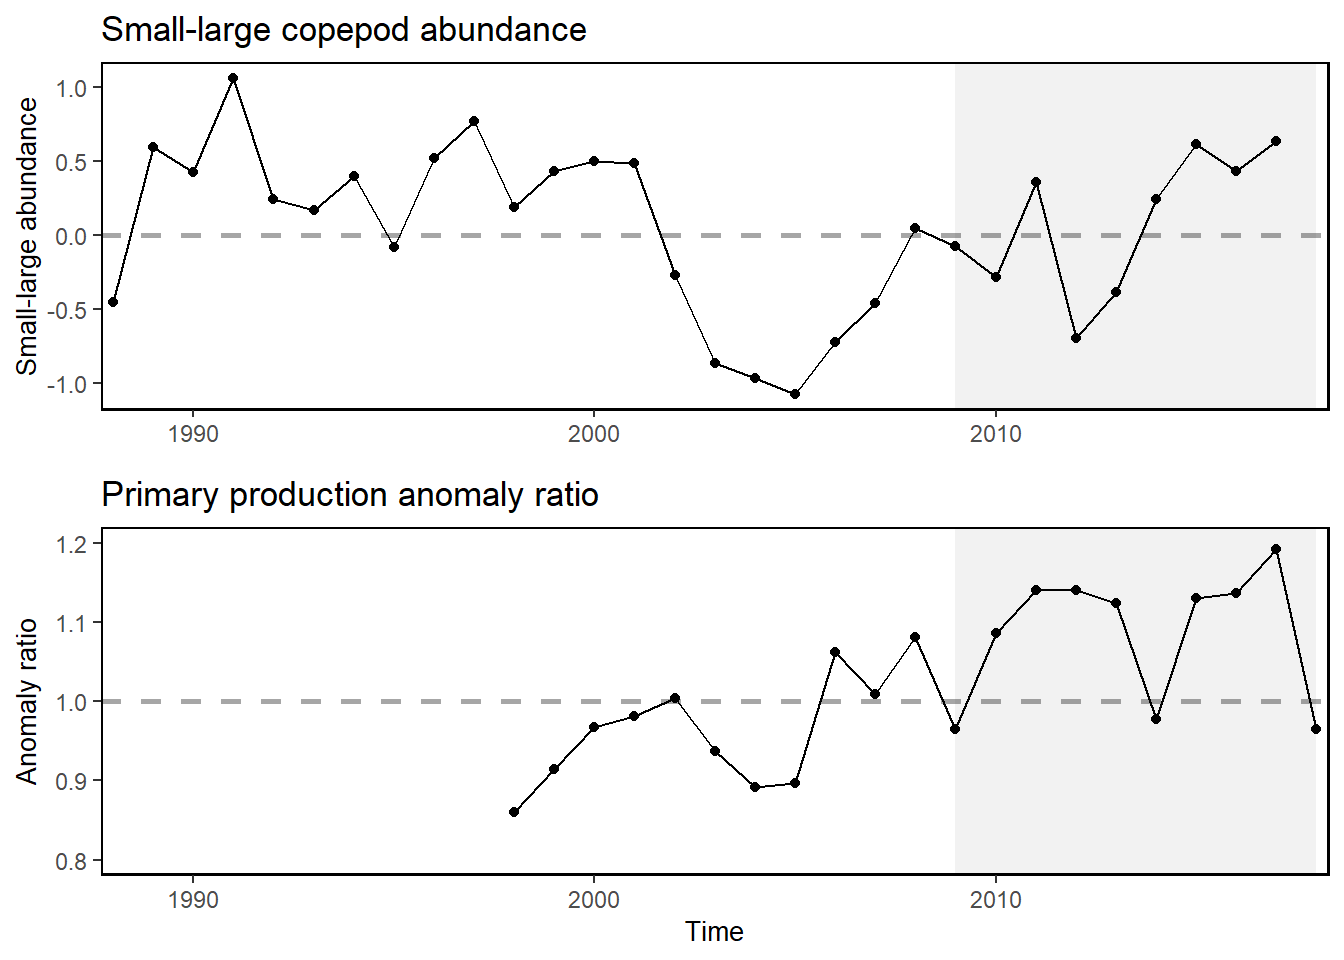
\includegraphics{C:/Users/kimberly.bastille/Desktop/tech-doc/imagesunnamed-chunk-16-1.pdf}
\caption{\label{fig:unnamed-chunk-16}MAB small-large zooplankton index and
the annual primary production anomaly.}
\end{figure}

Chl \emph{a} and primary production data were also examined in relation
to the long-term means of each series. The figure below shows data
specific to the Mid-Atlantic Bight.

\begin{Shaded}
\begin{Highlighting}[]
\NormalTok{interp_chl_pp <-}\StringTok{ }\ControlFlowTok{function}\NormalTok{(epu, }\DataTypeTok{year =} \DecValTok{2018}\NormalTok{, Variable)\{}
\NormalTok{  out <-}\StringTok{ }\NormalTok{ecodata}\OperatorTok{::}\NormalTok{chl_pp }\OperatorTok\StringTok{ }
\StringTok{    }\KeywordTok{filter}\NormalTok{(}\KeywordTok{str_detect}\NormalTok{(Var,Variable),}
\NormalTok{           EPU }\OperatorTok{==}\StringTok{ }\NormalTok{epu) }\OperatorTok\StringTok{ }
\StringTok{    }\KeywordTok{separate}\NormalTok{(.,Time, }\KeywordTok{c}\NormalTok{(}\StringTok{"Year"}\NormalTok{,}\StringTok{"Week"}\NormalTok{),}\DataTypeTok{sep =} \DecValTok{4}\NormalTok{) }\OperatorTok\StringTok{ }
\StringTok{    }\KeywordTok{filter}\NormalTok{(Year }\OperatorTok{==}\StringTok{ }\NormalTok{year) }\OperatorTok\StringTok{ }
\StringTok{    }\KeywordTok{group_by}\NormalTok{(EPU) }\OperatorTok\StringTok{ }
\StringTok{    }\KeywordTok{mutate}\NormalTok{(}\DataTypeTok{Time =} \DecValTok{1}\OperatorTok{:}\KeywordTok{length}\NormalTok{(Year))}
  
\NormalTok{  ltm_out <-}\StringTok{ }\NormalTok{ecodata}\OperatorTok{::}\NormalTok{chl_pp }\OperatorTok\StringTok{ }
\StringTok{    }\KeywordTok{filter}\NormalTok{(}\KeywordTok{str_detect}\NormalTok{(Var,Variable),}
\NormalTok{           EPU }\OperatorTok{==}\StringTok{ }\NormalTok{epu) }\OperatorTok\StringTok{ }
\StringTok{    }\KeywordTok{separate}\NormalTok{(.,Time, }\KeywordTok{c}\NormalTok{(}\StringTok{"Year"}\NormalTok{,}\StringTok{"Week"}\NormalTok{),}\DataTypeTok{sep =} \DecValTok{4}\NormalTok{) }\OperatorTok\StringTok{ }
\StringTok{    }\KeywordTok{group_by}\NormalTok{(Week) }\OperatorTok\StringTok{ }
\StringTok{    }\NormalTok{dplyr}\OperatorTok{::}\KeywordTok{summarise}\NormalTok{(}\DataTypeTok{LTM =} \KeywordTok{mean}\NormalTok{(Value, }\DataTypeTok{na.rm =}\NormalTok{ T),}
                     \DataTypeTok{SD =} \KeywordTok{sd}\NormalTok{(Value, }\DataTypeTok{na.rm =}\NormalTok{ T)) }\OperatorTok\StringTok{ }
\StringTok{    }\KeywordTok{mutate}\NormalTok{(}\DataTypeTok{Time =} \DecValTok{1}\OperatorTok{:}\KeywordTok{length}\NormalTok{(Week),}
           \DataTypeTok{sd.low =}\NormalTok{ LTM }\OperatorTok{-}\StringTok{ }\NormalTok{SD,}
           \DataTypeTok{sd.high =}\NormalTok{ LTM }\OperatorTok{+}\StringTok{ }\NormalTok{SD) }\OperatorTok\StringTok{ }
\StringTok{    }\KeywordTok{left_join}\NormalTok{(.,out, }\DataTypeTok{by =} \KeywordTok{c}\NormalTok{(}\StringTok{"Time"}\NormalTok{)) }\OperatorTok\StringTok{ }
\StringTok{    }\KeywordTok{mutate}\NormalTok{(}\DataTypeTok{status =} \KeywordTok{ifelse}\NormalTok{(Value }\OperatorTok{<}\StringTok{ }\NormalTok{sd.high }\OperatorTok{&}\StringTok{ }\NormalTok{Value }\OperatorTok{>}\StringTok{ }\NormalTok{sd.low, }\StringTok{"near_mean"}\NormalTok{,}
                           \KeywordTok{ifelse}\NormalTok{(Value }\OperatorTok{>}\StringTok{ }\NormalTok{sd.high, }\StringTok{"high"}\NormalTok{,}
                                  \KeywordTok{ifelse}\NormalTok{(Value }\OperatorTok{<}\StringTok{ }\NormalTok{sd.low,}\StringTok{"low"}\NormalTok{,}\OtherTok{NA}\NormalTok{))),}
           \DataTypeTok{group =} \StringTok{"PLOT"}\NormalTok{)}
  
  \KeywordTok{return}\NormalTok{(ltm_out)}
\NormalTok{\}}


\NormalTok{MAB_chl <-}\StringTok{ }\KeywordTok{interp_chl_pp}\NormalTok{(}\DataTypeTok{epu =} \StringTok{"MAB"}\NormalTok{, }\DataTypeTok{Variable =} \StringTok{"WEEKLY_CHLOR_A_MEDIAN MODIS-Aqua PAN"}\NormalTok{)}

\NormalTok{MAB_chl_weekly <-}\StringTok{ }\KeywordTok{ggplot}\NormalTok{(}\DataTypeTok{data =}\NormalTok{ MAB_chl) }\OperatorTok{+}
\StringTok{  }\KeywordTok{geom_line}\NormalTok{(}\KeywordTok{aes}\NormalTok{(}\DataTypeTok{x =}\NormalTok{ Time, }\DataTypeTok{y =}\NormalTok{ LTM)) }\OperatorTok{+}
\StringTok{  }\KeywordTok{geom_ribbon}\NormalTok{(}\KeywordTok{aes}\NormalTok{(}\DataTypeTok{x =}\NormalTok{ Time, }\DataTypeTok{ymin =}\NormalTok{ sd.low, }\DataTypeTok{ymax =}\NormalTok{ sd.high), }
              \DataTypeTok{alpha =} \FloatTok{0.1}\NormalTok{,}
              \DataTypeTok{fill =} \StringTok{"grey1"}\NormalTok{) }\OperatorTok{+}
\StringTok{  }\KeywordTok{geom_line}\NormalTok{(}\KeywordTok{aes}\NormalTok{(}\DataTypeTok{x =}\NormalTok{ Time, }\DataTypeTok{y =}\NormalTok{ Value),}
            \DataTypeTok{size =} \DecValTok{1}\NormalTok{,}\DataTypeTok{color =} \StringTok{"#33a02c"}\NormalTok{) }\OperatorTok{+}
\StringTok{  }\KeywordTok{ggtitle}\NormalTok{(}\KeywordTok{expression}\NormalTok{(}\StringTok{"Chlorophyll"}\OperatorTok{~}\KeywordTok{italic}\NormalTok{(a)}\OperatorTok{~}\StringTok{""}\NormalTok{)) }\OperatorTok{+}
\StringTok{  }\KeywordTok{guides}\NormalTok{(}\DataTypeTok{color =}\NormalTok{ F) }\OperatorTok{+}
\StringTok{  }\KeywordTok{xlab}\NormalTok{(}\StringTok{""}\NormalTok{)}\OperatorTok{+}
\StringTok{  }\KeywordTok{ylab}\NormalTok{(}\KeywordTok{expression}\NormalTok{(}\StringTok{"CHL (mg m"}\OperatorTok{^-}\DecValTok{3}\OperatorTok{*}\StringTok{")"}\NormalTok{)) }\OperatorTok{+}
\StringTok{  }\KeywordTok{scale_x_continuous}\NormalTok{(}\DataTypeTok{breaks =} \KeywordTok{seq}\NormalTok{(}\DecValTok{1}\NormalTok{,}\DecValTok{52}\NormalTok{,}\DecValTok{10}\NormalTok{),}
                   \DataTypeTok{labels =} \KeywordTok{c}\NormalTok{(}\StringTok{"Jan."}\NormalTok{,}\StringTok{"Mar."}\NormalTok{,}\StringTok{"May"}\NormalTok{,}\StringTok{"July"}\NormalTok{,}\StringTok{"Oct."}\NormalTok{,}\StringTok{"Dec."}\NormalTok{),}
                   \DataTypeTok{expand =} \KeywordTok{c}\NormalTok{(}\FloatTok{0.01}\NormalTok{,}\FloatTok{0.01}\NormalTok{)) }\OperatorTok{+}
\StringTok{  }\KeywordTok{scale_color_manual}\NormalTok{(}\DataTypeTok{values =} \KeywordTok{c}\NormalTok{(}\StringTok{"#ef8a62"}\NormalTok{,}\StringTok{"#2c7fb8"}\NormalTok{,}\StringTok{"#a1d99b"}\NormalTok{))}\OperatorTok{+}
\StringTok{  }\KeywordTok{theme_ts}\NormalTok{()}

\NormalTok{MAB_pp <-}\StringTok{ }\KeywordTok{interp_chl_pp}\NormalTok{(}\DataTypeTok{epu =} \StringTok{"MAB"}\NormalTok{, }\DataTypeTok{Variable =}  \StringTok{"WEEKLY_PPD_MEDIAN"}\NormalTok{)}

\NormalTok{MAB_pp_weekly <-}\StringTok{ }\KeywordTok{ggplot}\NormalTok{(}\DataTypeTok{data =}\NormalTok{ MAB_pp) }\OperatorTok{+}
\StringTok{  }\KeywordTok{geom_line}\NormalTok{(}\KeywordTok{aes}\NormalTok{(}\DataTypeTok{x =}\NormalTok{ Time, }\DataTypeTok{y =}\NormalTok{ LTM)) }\OperatorTok{+}
\StringTok{  }\KeywordTok{geom_ribbon}\NormalTok{(}\KeywordTok{aes}\NormalTok{(}\DataTypeTok{x =}\NormalTok{ Time, }\DataTypeTok{ymin =}\NormalTok{ sd.low, }\DataTypeTok{ymax =}\NormalTok{ sd.high),}
              \DataTypeTok{alpha =} \FloatTok{0.1}\NormalTok{,}
              \DataTypeTok{fill =} \StringTok{"grey1"}\NormalTok{) }\OperatorTok{+}
\StringTok{  }\KeywordTok{geom_line}\NormalTok{(}\KeywordTok{aes}\NormalTok{(}\DataTypeTok{x =}\NormalTok{ Time, }\DataTypeTok{y =}\NormalTok{ Value),}
            \DataTypeTok{size =} \DecValTok{1}\NormalTok{,}\DataTypeTok{color =} \StringTok{"#33a02c"}\NormalTok{) }\OperatorTok{+}
\StringTok{  }\KeywordTok{ggtitle}\NormalTok{(}\KeywordTok{expression}\NormalTok{(}\StringTok{"Primary production"}\NormalTok{)) }\OperatorTok{+}
\StringTok{  }\KeywordTok{guides}\NormalTok{(}\DataTypeTok{color =}\NormalTok{ F) }\OperatorTok{+}
\StringTok{  }\KeywordTok{xlab}\NormalTok{(}\StringTok{""}\NormalTok{)}\OperatorTok{+}
\StringTok{  }\KeywordTok{ylab}\NormalTok{(}\KeywordTok{expression}\NormalTok{(}\StringTok{"PP (gC m"}\OperatorTok{^-}\DecValTok{2}\OperatorTok{*}\StringTok{" d"}\OperatorTok{^-}\DecValTok{1}\OperatorTok{*}\StringTok{")"}\NormalTok{)) }\OperatorTok{+}
\StringTok{  }\KeywordTok{scale_x_continuous}\NormalTok{(}\DataTypeTok{breaks =} \KeywordTok{seq}\NormalTok{(}\DecValTok{1}\NormalTok{,}\DecValTok{52}\NormalTok{,}\DecValTok{10}\NormalTok{),}
                   \DataTypeTok{labels =} \KeywordTok{c}\NormalTok{(}\StringTok{"Jan."}\NormalTok{,}\StringTok{"Mar."}\NormalTok{,}\StringTok{"May"}\NormalTok{,}\StringTok{"July"}\NormalTok{,}\StringTok{"Oct."}\NormalTok{,}\StringTok{"Dec."}\NormalTok{),}
                   \DataTypeTok{expand =} \KeywordTok{c}\NormalTok{(}\FloatTok{0.01}\NormalTok{,}\FloatTok{0.01}\NormalTok{)) }\OperatorTok{+}
\StringTok{  }\KeywordTok{scale_color_manual}\NormalTok{(}\DataTypeTok{values =} \KeywordTok{c}\NormalTok{(}\StringTok{"#ef8a62"}\NormalTok{,}\StringTok{"#2c7fb8"}\NormalTok{,}\StringTok{"#a1d99b"}\NormalTok{))}\OperatorTok{+}
\StringTok{  }\KeywordTok{theme_ts}\NormalTok{()}

\CommentTok{#MAB_chl_weekly + MAB_pp_weekly + plot_layout(ncol = 1)}
\NormalTok{MAB_chl_weekly}
\end{Highlighting}
\end{Shaded}

\begin{figure}
\centering
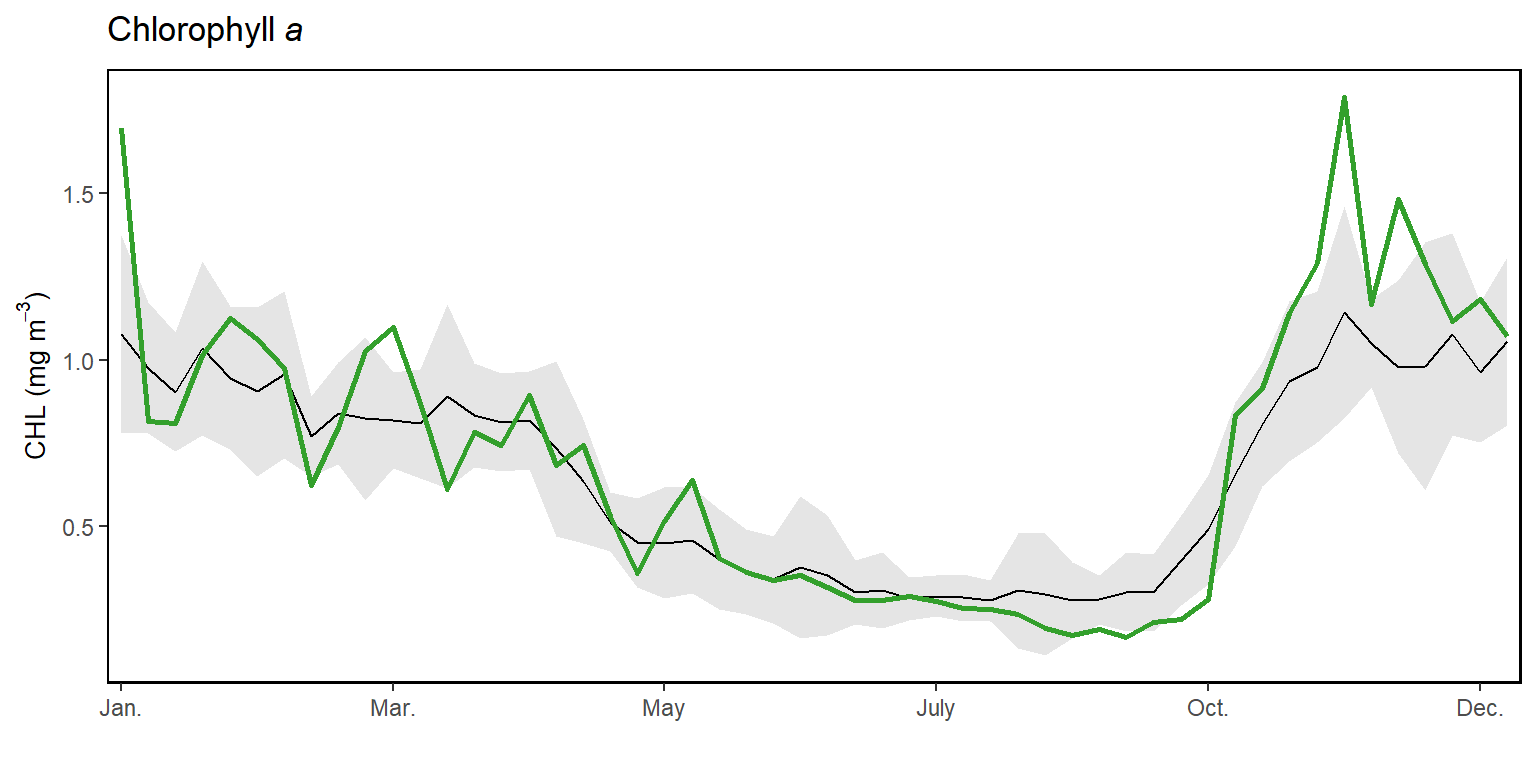
\includegraphics{C:/Users/kimberly.bastille/Desktop/tech-doc/imagesunnamed-chunk-17-1.pdf}
\caption{\label{fig:unnamed-chunk-17}Weekly chlorophyll concentrations in
the Mid-Atlantic are shown by the colored line for 2018. The long-term
mean is shown in black, and shading indicates +/- 1 sample SD.}
\end{figure}

In the figure below, we show monthly primary productivity on an annual
time step in the Mid-Atlantic Bight.

\begin{Shaded}
\begin{Highlighting}[]
\NormalTok{out_pp <-}\StringTok{ }\NormalTok{ecodata}\OperatorTok{::}\NormalTok{chl_pp }\OperatorTok\StringTok{ }
\StringTok{  }\KeywordTok{filter}\NormalTok{(EPU }\OperatorTok{==}\StringTok{ "MAB"}\NormalTok{,}
         \KeywordTok{str_detect}\NormalTok{(Var, }\StringTok{"MONTHLY_PPD_MEDIAN"}\NormalTok{)) }\OperatorTok\StringTok{ }
\StringTok{  }\KeywordTok{separate}\NormalTok{(.,Time, }\DataTypeTok{into =} \KeywordTok{c}\NormalTok{(}\StringTok{"Year"}\NormalTok{,}\StringTok{"Month"}\NormalTok{), }\DataTypeTok{sep =} \DecValTok{4}\NormalTok{) }\OperatorTok\StringTok{ }
\StringTok{    }\KeywordTok{mutate}\NormalTok{(}\DataTypeTok{Month =}\NormalTok{ plyr}\OperatorTok{::}\KeywordTok{mapvalues}\NormalTok{(Month, }\DataTypeTok{from =} \KeywordTok{c}\NormalTok{(}\StringTok{"01"}\NormalTok{,}\StringTok{"02"}\NormalTok{,}\StringTok{"03"}\NormalTok{,}\StringTok{"04"}\NormalTok{,}\StringTok{"05"}\NormalTok{,}\StringTok{"06"}\NormalTok{,}
                                                   \StringTok{"07"}\NormalTok{,}\StringTok{"08"}\NormalTok{,}\StringTok{"09"}\NormalTok{,}\StringTok{"10"}\NormalTok{,}\StringTok{"11"}\NormalTok{,}\StringTok{"12"}\NormalTok{),}
                                   \DataTypeTok{to =} \KeywordTok{c}\NormalTok{(month.abb))) }\OperatorTok\StringTok{ }
\StringTok{  }\KeywordTok{group_by}\NormalTok{(Month) }\OperatorTok\StringTok{ }
\StringTok{  }\KeywordTok{mutate}\NormalTok{(}\DataTypeTok{hline =} \KeywordTok{mean}\NormalTok{(Value))}
\NormalTok{out_pp}\OperatorTok{$}\NormalTok{Month <-}\StringTok{ }\KeywordTok{factor}\NormalTok{(out_pp}\OperatorTok{$}\NormalTok{Month, }\DataTypeTok{levels =}\NormalTok{ month.abb)}


\NormalTok{(pp_cci <-}\StringTok{ }\KeywordTok{ggplot}\NormalTok{(out_pp) }\OperatorTok{+}\StringTok{  }
\StringTok{   }\CommentTok{# geom_gls(aes(x = Year, y = Value, group = Month))+}
\StringTok{    }\KeywordTok{geom_point}\NormalTok{(}\KeywordTok{aes}\NormalTok{(}\DataTypeTok{x =}\NormalTok{ Year, }\DataTypeTok{y =}\NormalTok{ Value, }\DataTypeTok{group =}\NormalTok{ Month)) }\OperatorTok{+}
\StringTok{    }\KeywordTok{geom_line}\NormalTok{(}\KeywordTok{aes}\NormalTok{(}\DataTypeTok{x =}\NormalTok{ Year, }\DataTypeTok{y =}\NormalTok{ Value, }\DataTypeTok{group =}\NormalTok{ Month)) }\OperatorTok{+}
\StringTok{    }\KeywordTok{scale_x_discrete}\NormalTok{(}\DataTypeTok{name =} \StringTok{"Time"}\NormalTok{, }\DataTypeTok{breaks =} \KeywordTok{seq}\NormalTok{(}\KeywordTok{min}\NormalTok{(out_pp}\OperatorTok{$}\NormalTok{Year),}\KeywordTok{max}\NormalTok{(out_pp}\OperatorTok{$}\NormalTok{Year),}\DecValTok{10}\NormalTok{)) }\OperatorTok{+}\StringTok{  }
\StringTok{        }\KeywordTok{geom_hline}\NormalTok{(}\KeywordTok{aes}\NormalTok{(}\DataTypeTok{yintercept =}\NormalTok{ hline),}
           \DataTypeTok{size =}\NormalTok{ hline.size,}
           \DataTypeTok{alpha =}\NormalTok{ hline.alpha,}
           \DataTypeTok{linetype =}\NormalTok{ hline.lty) }\OperatorTok{+}
\StringTok{    }\KeywordTok{facet_wrap}\NormalTok{(Month}\OperatorTok{~}\NormalTok{., }\DataTypeTok{ncol =} \DecValTok{6}\NormalTok{) }\OperatorTok{+}
\StringTok{    }\KeywordTok{ggtitle}\NormalTok{(}\StringTok{"Monthly median PPD"}\NormalTok{) }\OperatorTok{+}
\StringTok{    }\KeywordTok{ylab}\NormalTok{(}\KeywordTok{expression}\NormalTok{(}\StringTok{"PP (gC m"}\OperatorTok{^-}\DecValTok{2}\OperatorTok{*}\StringTok{" d"}\OperatorTok{^-}\DecValTok{1}\OperatorTok{*}\StringTok{")"}\NormalTok{)) }\OperatorTok{+}
\StringTok{    }\KeywordTok{theme_facet}\NormalTok{() }\OperatorTok{+}
\StringTok{    }\KeywordTok{theme}\NormalTok{(}\DataTypeTok{axis.text.x =} \KeywordTok{element_text}\NormalTok{(}\DataTypeTok{angle=}\DecValTok{45}\NormalTok{, }\DataTypeTok{hjust =} \DecValTok{1}\NormalTok{),}
          \DataTypeTok{panel.spacing =} \KeywordTok{unit}\NormalTok{(}\DecValTok{1}\NormalTok{, }\StringTok{"lines"}\NormalTok{),}
          \DataTypeTok{plot.margin =} \KeywordTok{unit}\NormalTok{(}\KeywordTok{c}\NormalTok{(}\FloatTok{0.1}\NormalTok{, }\DecValTok{0}\NormalTok{, }\DecValTok{0}\NormalTok{, }\DecValTok{0}\NormalTok{), }\StringTok{"cm"}\NormalTok{)))}
\end{Highlighting}
\end{Shaded}

\begin{figure}
\centering
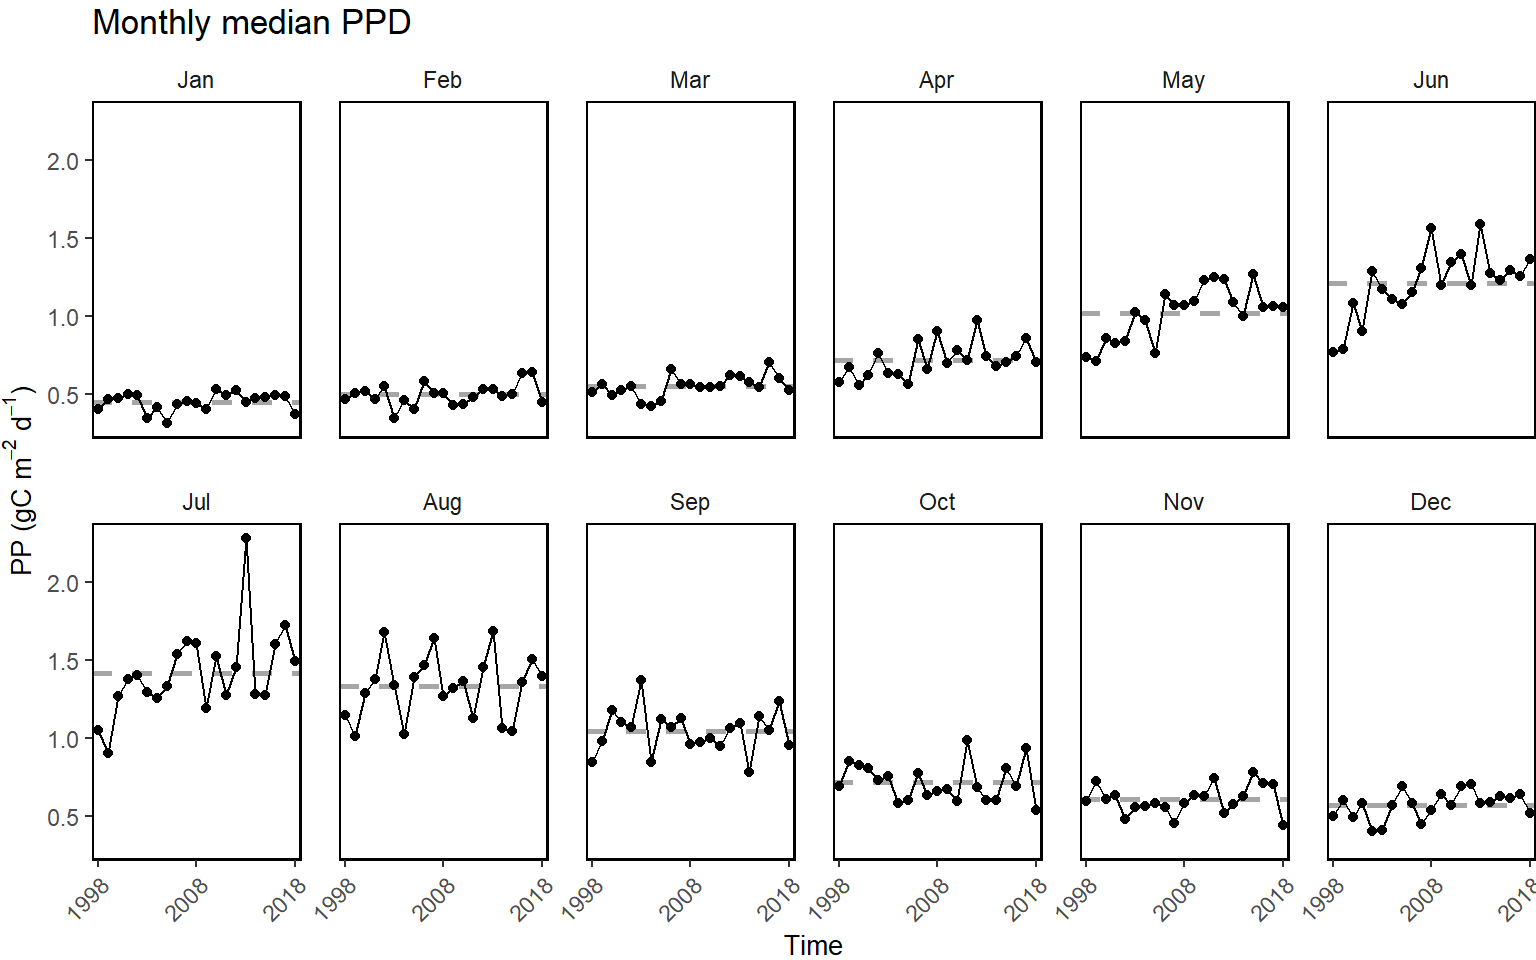
\includegraphics{C:/Users/kimberly.bastille/Desktop/tech-doc/imagesunnamed-chunk-18-1.pdf}
\caption{\label{fig:unnamed-chunk-18}Monthly primary production trends show
the annual cycle (i.e.~the peak during the summer months) and the
changes over time for each month.}
\end{figure}

\chapter{Fishing Community Climate
Vulnerability}\label{fishing-community-climate-vulnerability}

\textbf{Description}: Community climate vulnerability

\textbf{Found in}: State of the Ecosystem - Gulf of Maine \& Georges
Bank (2018), State of the Ecosystem - Mid-Atlantic (2018)

\textbf{Indicator category}: Database pull with analysis

\textbf{Contributor(s)}: Lisa L. Colburn

\textbf{Data steward}: Lisa L. Colburn

\textbf{Point of contact}: Lisa L. Colburn

\textbf{Public availability statement}: The fisheries data used for this
analysis includes confidential information and is not available to the
public.

\section{Methods}\label{methods-8}

\subsection{Data sources}\label{data-sources-8}

The data used in community climate vulnerability analyses were derived
from the following sources in partnership with the Atlantic Coastal
Cooperative Statistics Program's (ACCSP) Standard Atlantic Fisheries
Information System (SAFIS).

\begin{longtable}[]{@{}ll@{}}
\toprule
\begin{minipage}[b]{0.35\columnwidth}\raggedright\strut
Database Name\strut
\end{minipage} & \begin{minipage}[b]{0.51\columnwidth}\raggedright\strut
Description\strut
\end{minipage}\tabularnewline
\midrule
\endhead
\begin{minipage}[t]{0.35\columnwidth}\raggedright\strut
Cfdersyyyy\strut
\end{minipage} & \begin{minipage}[t]{0.51\columnwidth}\raggedright\strut
The dealer data are transaction-level pricing at the level of the
``market-category.'' These data are primarily generated through
mandatory reporting by federally-permitted fish dealers. The federal
reporting is supplemented with data from non-federally-permitted
(state-only) fish dealers. Data are currently reported electronically in
partnership with ACCSP through SAFIS.\strut
\end{minipage}\tabularnewline
\begin{minipage}[t]{0.35\columnwidth}\raggedright\strut
Cfvessyyy\strut
\end{minipage} & \begin{minipage}[t]{0.51\columnwidth}\raggedright\strut
A related database that contains permit information.\strut
\end{minipage}\tabularnewline
\bottomrule
\end{longtable}

In these databases, the variable ``port'' contains the post associated
with the vessel. The variable ``Statenm'' refers to the state of the
mailing address of the owner.

\subsection{Data extraction}\label{data-extraction-7}

\begin{Shaded}
\begin{Highlighting}[]
\KeywordTok{create} \KeywordTok{table}\NormalTok{ cfders2011 }\KeywordTok{as}
\KeywordTok{select}\NormalTok{ *}
\KeywordTok{from}\NormalTok{ connection }\KeywordTok{to}\NormalTok{ oracle}
\NormalTok{(}\KeywordTok{select}\NormalTok{ port, state, }\DataTypeTok{year}\NormalTok{, dealnum, permit, nespp3, spplndlb, sppvalue }\KeywordTok{from}\NormalTok{ cfders2011 }\KeywordTok{where}\NormalTok{ permit > }\DecValTok{0} \KeywordTok{order} \KeywordTok{by}\NormalTok{ permit);}
\KeywordTok{create} \KeywordTok{table}\NormalTok{ cfvess11 }\KeywordTok{as}
\KeywordTok{select}\NormalTok{ *}
\KeywordTok{from}\NormalTok{ connection }\KeywordTok{to}\NormalTok{ oracle}
\NormalTok{(}\KeywordTok{select}\NormalTok{ permit, homeport, homest }\KeywordTok{from}\NormalTok{ CFDBS.cfvess11 }\KeywordTok{where}\NormalTok{ permit > }\DecValTok{0} \KeywordTok{order} \KeywordTok{by}\NormalTok{ permit);}
\KeywordTok{create} \KeywordTok{table}\NormalTok{ port_name }\KeywordTok{as}
\KeywordTok{select}\NormalTok{ *}
\KeywordTok{from}\NormalTok{ connection }\KeywordTok{to}\NormalTok{ oracle}
\NormalTok{(}\KeywordTok{select}\NormalTok{ port, portnm }\KeywordTok{from}\NormalTok{ port }\KeywordTok{order} \KeywordTok{by}\NormalTok{ port);}
\KeywordTok{create} \KeywordTok{table}\NormalTok{ st_name }\KeywordTok{as}
\KeywordTok{select}\NormalTok{ *}
\KeywordTok{from}\NormalTok{ connection }\KeywordTok{to}\NormalTok{ oracle}
\NormalTok{(}\KeywordTok{select}\NormalTok{ state, stateabb }\KeywordTok{from}\NormalTok{ statenm }\KeywordTok{order} \KeywordTok{by}\NormalTok{ state);}

\NormalTok{Truncated SAS code:}
\CommentTok{/*CREATE VARIABLES FOR TOTAL LANDINGS WEIGTH AND VALUE (SUM) BY PORT OF LANDING AND BY HOMEPORT*/}
\KeywordTok{data}\NormalTok{ landings_ports1; }\KeywordTok{set}\NormalTok{ landings_ports;}
\NormalTok{run;}
\NormalTok{proc }\KeywordTok{sort}\NormalTok{;}
\KeywordTok{by}\NormalTok{ port state;}
\NormalTok{run;}
\NormalTok{proc means noprint }\KeywordTok{data}\NormalTok{ = landings_ports1; }\KeywordTok{by}\NormalTok{ port state; }
\NormalTok{var spplndlb sppvalue;}
\KeywordTok{id}\NormalTok{ port state;}
\NormalTok{output }\KeywordTok{out}\NormalTok{ = landport_totspp }\FunctionTok{sum}\NormalTok{ = L_Totlb L_Totval;}
\NormalTok{run;}
\NormalTok{proc }\KeywordTok{sort}\NormalTok{;}
\KeywordTok{by}\NormalTok{ port;}
\NormalTok{run;}
\KeywordTok{data}\NormalTok{ landings_ports2; }\KeywordTok{set}\NormalTok{ landings_ports;}
\NormalTok{run;}
\NormalTok{proc }\KeywordTok{sort}\NormalTok{;}
\KeywordTok{by}\NormalTok{ homeport homest;}
\NormalTok{run;}
\NormalTok{proc means noprint }\KeywordTok{data}\NormalTok{ = landings_ports2; }\KeywordTok{by}\NormalTok{ homeport homest; }
\NormalTok{var spplndlb sppvalue;}
\KeywordTok{id}\NormalTok{ homeport homest;}
\NormalTok{output }\KeywordTok{out}\NormalTok{ = homeport_totspp }\FunctionTok{sum}\NormalTok{ = H_Totlb H_Totval;}
\NormalTok{run;}
\NormalTok{proc }\KeywordTok{sort}\NormalTok{;}
\KeywordTok{by}\NormalTok{ homeport;}
\NormalTok{run;}
\CommentTok{/*CREATE SPECIES VARIABLES*/}
\KeywordTok{data}\NormalTok{ landings_ports_NE_spp; }\KeywordTok{set}\NormalTok{ landings_ports;}
\NormalTok{monklb = }\DecValTok{0}\NormalTok{; monkval = }\DecValTok{0}\NormalTok{; }\CommentTok{/*monkfish*/}
\NormalTok{bluelb = }\DecValTok{0}\NormalTok{; blueval = }\DecValTok{0}\NormalTok{; }\CommentTok{/*bluefish*/}
\NormalTok{.omitted.}
\NormalTok{otherlb = }\DecValTok{0}\NormalTok{; otherval = }\DecValTok{0}\NormalTok{; }\CommentTok{/*other - everything else*/}
\NormalTok{run;}
\KeywordTok{data}\NormalTok{ landings_ports_NE_spp2; }\KeywordTok{set}\NormalTok{ landings_ports_NE_spp;}
\KeywordTok{if}\NormalTok{ nespp3 = }\DecValTok{012} \KeywordTok{then}\NormalTok{ do; monklb = spplndlb; monkval = sppvalue; }\KeywordTok{end}\NormalTok{;}
\NormalTok{...ommitted.}
\KeywordTok{if}\NormalTok{ nespp3 = }\DecValTok{406} \KeywordTok{then}\NormalTok{ do; spotlb = spplndlb; spotval = sppvalue; }\KeywordTok{end}\NormalTok{;}
\KeywordTok{if}\NormalTok{ nespp3 }\KeywordTok{not} \KeywordTok{in}\NormalTok{ (}\DecValTok{012}\NormalTok{, }\DecValTok{023}\NormalTok{, }\DecValTok{033}\NormalTok{, }\DecValTok{051}\NormalTok{, }\DecValTok{081}\NormalTok{, }\DecValTok{105}\NormalTok{, }\DecValTok{112}\NormalTok{, }\DecValTok{115}\NormalTok{, }\DecValTok{116}\NormalTok{, }\DecValTok{120}\NormalTok{, }\DecValTok{121}\NormalTok{, }\DecValTok{122}\NormalTok{, }\DecValTok{123}\NormalTok{, }\DecValTok{124}\NormalTok{, }\DecValTok{125}\NormalTok{, }\DecValTok{132}\NormalTok{, }\DecValTok{147}\NormalTok{, }\DecValTok{152}\NormalTok{, }\DecValTok{153}\NormalTok{, }\DecValTok{155}\NormalTok{, }\DecValTok{159}\NormalTok{, }\DecValTok{168}\NormalTok{, }\DecValTok{194}\NormalTok{, }\DecValTok{197}\NormalTok{, }\DecValTok{212}\NormalTok{, }
\DecValTok{221}\NormalTok{, }\DecValTok{240}\NormalTok{, }\DecValTok{250}\NormalTok{, }\DecValTok{269}\NormalTok{, }\DecValTok{305}\NormalTok{, }\DecValTok{329}\NormalTok{, }\DecValTok{330}\NormalTok{, }\DecValTok{335}\NormalTok{, }\DecValTok{344}\NormalTok{, }\DecValTok{345}\NormalTok{, }\DecValTok{351}\NormalTok{, }\DecValTok{352}\NormalTok{, }\DecValTok{365}\NormalTok{, }\DecValTok{366}\NormalTok{, }\DecValTok{367}\NormalTok{, }\DecValTok{368}\NormalTok{, }\DecValTok{369}\NormalTok{, }\DecValTok{370}\NormalTok{, }\DecValTok{372}\NormalTok{, }\DecValTok{373}\NormalTok{, }\DecValTok{384}\NormalTok{, }\DecValTok{415}\NormalTok{, }\DecValTok{418}\NormalTok{, }\DecValTok{432}\NormalTok{, }\DecValTok{438}\NormalTok{, }\DecValTok{443}\NormalTok{, }\DecValTok{444}\NormalTok{, }\DecValTok{445}\NormalTok{, }
\DecValTok{446}\NormalTok{, }\DecValTok{447}\NormalTok{, }\DecValTok{464}\NormalTok{, }\DecValTok{466}\NormalTok{, }\DecValTok{467}\NormalTok{, }\DecValTok{468}\NormalTok{, }\DecValTok{469}\NormalTok{, }\DecValTok{470}\NormalTok{, }\DecValTok{471}\NormalTok{, }\DecValTok{472}\NormalTok{, }\DecValTok{507}\NormalTok{, }\DecValTok{508}\NormalTok{, }\DecValTok{509}\NormalTok{, }\DecValTok{512}\NormalTok{, }\DecValTok{517}\NormalTok{, }\DecValTok{700}\NormalTok{, }\DecValTok{710}\NormalTok{, }\DecValTok{711}\NormalTok{, }\DecValTok{724}\NormalTok{, }\DecValTok{727}\NormalTok{, }\DecValTok{748}\NormalTok{, }\DecValTok{754}\NormalTok{, }\DecValTok{769}\NormalTok{, }\DecValTok{774}\NormalTok{, }\DecValTok{775}\NormalTok{, }\DecValTok{781}\NormalTok{, }\DecValTok{786}\NormalTok{, }\DecValTok{789}\NormalTok{, }
\DecValTok{798}\NormalTok{, }\DecValTok{799}\NormalTok{, }\DecValTok{800}\NormalTok{, }\DecValTok{801}\NormalTok{, }\DecValTok{802}\NormalTok{, }\DecValTok{805}\NormalTok{, }\DecValTok{806}\NormalTok{, }\DecValTok{899}\NormalTok{, }\DecValTok{001}\NormalTok{, }\DecValTok{090}\NormalTok{, }\DecValTok{069}\NormalTok{, }\DecValTok{107}\NormalTok{, }\DecValTok{150}\NormalTok{, }\DecValTok{173}\NormalTok{, }\DecValTok{196}\NormalTok{, }\DecValTok{334}\NormalTok{, }\DecValTok{347}\NormalTok{, }\DecValTok{349}\NormalTok{, }\DecValTok{364}\NormalTok{, }\DecValTok{371}\NormalTok{, }\DecValTok{420}\NormalTok{, }\DecValTok{422}\NormalTok{, }\DecValTok{481}\NormalTok{, }\DecValTok{484}\NormalTok{, }\DecValTok{714}\NormalTok{, }\DecValTok{776}\NormalTok{, }\DecValTok{777}\NormalTok{, }\DecValTok{823}\NormalTok{, }\DecValTok{763}\NormalTok{, }\DecValTok{736}\NormalTok{) }
\KeywordTok{then}\NormalTok{ do; otherlb = spplndlb; otherval = sppvalue; }\KeywordTok{end}\NormalTok{;}
\NormalTok{run; }
\CommentTok{/*SUM SPECIES LANDINGS BY PORT OF LANDING*/}
\NormalTok{proc }\KeywordTok{sort}\NormalTok{; }\KeywordTok{by}\NormalTok{ port; proc means noprint }\KeywordTok{data}\NormalTok{ = landings_ports_NE_spp2; }\KeywordTok{by}\NormalTok{ port state; }
\NormalTok{. omitted ...}
\KeywordTok{id}\NormalTok{ port state;}
\NormalTok{output }\KeywordTok{out}\NormalTok{ = spp_porlnd_NE }\FunctionTok{sum}\NormalTok{ = ;}
\NormalTok{run;}
\NormalTok{proc }\KeywordTok{sort}\NormalTok{;}
\KeywordTok{by}\NormalTok{ port;}
\NormalTok{run;}
\CommentTok{/*SUM SPECIES LANDINGS BY HOMEPORT*/}
\KeywordTok{data}\NormalTok{ spp_home; }\KeywordTok{set}\NormalTok{ landings_ports_NE_spp2;}
\NormalTok{run;}
\NormalTok{proc }\KeywordTok{sort}\NormalTok{; }\KeywordTok{by}\NormalTok{ homeport homest; proc means noprint }\KeywordTok{data}\NormalTok{ = spp_home; }\KeywordTok{by}\NormalTok{ homeport homest; }
\NormalTok{. species are counted..}
\KeywordTok{id}\NormalTok{ homeport homest;}
\NormalTok{output }\KeywordTok{out}\NormalTok{ = spp_homep_NE }\FunctionTok{sum}\NormalTok{ = ;}
\NormalTok{run}
\NormalTok{proc }\KeywordTok{sort}\NormalTok{;}
\KeywordTok{by}\NormalTok{ homeport; run;}
\CommentTok{/*MERGE TOTAL PERMITS AND TOTAL DEALERS BY PORT OF LANDING*/}
\KeywordTok{data}\NormalTok{ land_port_totperm2; }\KeywordTok{set}\NormalTok{ land_port_totperm;}
\NormalTok{run;}
\NormalTok{proc }\KeywordTok{sort}\NormalTok{;}
\KeywordTok{by}\NormalTok{ port; run;}
\KeywordTok{data}\NormalTok{ lnd_port_permit; }\KeywordTok{merge}\NormalTok{ spp_porlnd_NE (IN=X) land_port_totperm2 (IN=Y);}
\KeywordTok{by}\NormalTok{ port; }\KeywordTok{if}\NormalTok{ X=}\DecValTok{1}\NormalTok{; run;}\KeywordTok{data}\NormalTok{ land_port_totdeal2; }\KeywordTok{set}\NormalTok{ land_port_totdeal;}
\NormalTok{run;}
\NormalTok{proc }\KeywordTok{sort}\NormalTok{;}
\KeywordTok{by}\NormalTok{ port;}
\NormalTok{run;}
\KeywordTok{data}\NormalTok{ lnd_port_permit_deal; }\KeywordTok{merge}\NormalTok{ lnd_port_permit (IN=x) land_port_totdeal2 (IN=Y);}
\KeywordTok{by}\NormalTok{ port; }\KeywordTok{if}\NormalTok{ X=}\DecValTok{1}\NormalTok{; run;}
\CommentTok{/*MERGE WITH PORT NAME AND STATE ABBREVIATION*/}
\KeywordTok{data}\NormalTok{ lnd_port_permit_deal_nm; }\KeywordTok{merge}\NormalTok{ lnd_port_permit_deal (IN=X) port_name (IN=Y);}
\KeywordTok{by}\NormalTok{ port; }\KeywordTok{if}\NormalTok{ X=}\DecValTok{1}\NormalTok{; run;}
\KeywordTok{data}\NormalTok{ lnd_port_permit_deal_nm_st; }\KeywordTok{merge}\NormalTok{ lnd_port_permit_deal_nm (IN=x) st_name (IN=Y); proc }\KeywordTok{sort}\NormalTok{;}
\KeywordTok{by}\NormalTok{ port; }\KeywordTok{if}\NormalTok{ X=}\DecValTok{1}\NormalTok{; run;}
\CommentTok{/*MERGE TOTAL PERMITS AND TOTAL DEALERS BY HOMEPORT*/}
\KeywordTok{data}\NormalTok{ home_port_totperm2; }\KeywordTok{set}\NormalTok{ home_port_totperm;}
\NormalTok{run;}
\NormalTok{proc }\KeywordTok{sort}\NormalTok{;}
\KeywordTok{by}\NormalTok{ homeport;}
\NormalTok{run;}
\KeywordTok{data}\NormalTok{ home_port_permit; }\KeywordTok{merge}\NormalTok{ spp_homep_NE (IN=X) home_port_totperm2 (IN=Y);}
\KeywordTok{by}\NormalTok{ homeport; }\KeywordTok{if}\NormalTok{ X=}\DecValTok{1}\NormalTok{; run; }\KeywordTok{data}\NormalTok{ home_port_totdeal2; }\KeywordTok{set}\NormalTok{ home_port_totdeal;}
\NormalTok{run;}
\NormalTok{proc }\KeywordTok{sort}\NormalTok{;}
\KeywordTok{by}\NormalTok{ homeport;}
\NormalTok{run;}
\KeywordTok{data}\NormalTok{ home_port_permit_deal; }\KeywordTok{merge}\NormalTok{ home_port_permit (IN=x) home_port_totdeal2 (IN=Y);}
\KeywordTok{by}\NormalTok{ homeport; }\KeywordTok{if}\NormalTok{ X=}\DecValTok{1}\NormalTok{; run; proc }\KeywordTok{sort}\NormalTok{;}
\KeywordTok{by}\NormalTok{ homeport;}
\NormalTok{run;}
\CommentTok{/*MERGE TOTAL LANDINGS BY PORT OF LANDING*/}
\KeywordTok{data}\NormalTok{ lnd_port_per_deal_nm_st_tspp; }\KeywordTok{merge}\NormalTok{ lnd_port_permit_deal_nm_st (IN=X) landport_totspp (IN=Y);}
\KeywordTok{by}\NormalTok{ port; }\KeywordTok{if}\NormalTok{ X=}\DecValTok{1}\NormalTok{; run;}
\CommentTok{/*MERGE TOTAL LANDINGS BY HOMEPORT*/}
\KeywordTok{data}\NormalTok{ home_port_per_deal_tspp; }\KeywordTok{merge}\NormalTok{ home_port_permit_deal (IN=X) homeport_totspp (IN=Y);}
\KeywordTok{by}\NormalTok{ homeport; }\KeywordTok{if}\NormalTok{ X=}\DecValTok{1}\NormalTok{; run;}
\KeywordTok{data}\NormalTok{ netana.port_landing11; }\KeywordTok{set}\NormalTok{ lnd_port_per_deal_nm_st_tspp;}
\KeywordTok{if}\NormalTok{ state }\KeywordTok{in}\NormalTok{ (}\DecValTok{22}\NormalTok{, }\DecValTok{32}\NormalTok{, }\DecValTok{24}\NormalTok{, }\DecValTok{42}\NormalTok{, }\DecValTok{7}\NormalTok{, }\DecValTok{35}\NormalTok{, }\DecValTok{33}\NormalTok{, }\DecValTok{8}\NormalTok{, }\DecValTok{23}\NormalTok{, }\DecValTok{49}\NormalTok{, }\DecValTok{36}\NormalTok{);}
\NormalTok{run;}
\NormalTok{proc }\KeywordTok{sort}\NormalTok{;}
\KeywordTok{by}\NormalTok{ port state;}
\NormalTok{run;}
\KeywordTok{data}\NormalTok{ netana.homeport11; }\KeywordTok{set}\NormalTok{ home_port_per_deal_tspp;}
\KeywordTok{if}\NormalTok{ homest }\KeywordTok{in}\NormalTok{ (}\StringTok{'ME'}\NormalTok{, }\StringTok{'NH'}\NormalTok{, }\StringTok{'MA'}\NormalTok{, }\StringTok{'RI'}\NormalTok{, }\StringTok{'CT'}\NormalTok{, }\StringTok{'NY'}\NormalTok{, }\StringTok{'NJ'}\NormalTok{, }\StringTok{'DE'}\NormalTok{, }\StringTok{'MD'}\NormalTok{, }\StringTok{'VA'}\NormalTok{, }\StringTok{'NC'}\NormalTok{);}
\NormalTok{run;}
\NormalTok{proc }\KeywordTok{sort}\NormalTok{;}
\KeywordTok{by}\NormalTok{ homeport homest;}
\NormalTok{run;}
\end{Highlighting}
\end{Shaded}

\subsection{Data analysis}\label{data-analysis-7}

The results described below were developed using the methodology
described in Colburn et al.
(\protect\hyperlink{ref-colburn_indicators_2016}{2016}).

\begin{enumerate}
\def\labelenumi{\arabic{enumi}.}
\tightlist
\item
  \emph{Mapping community climate vulnerability} - The map was produced
  using two variables: total value landed in a community and community
  species vulnerability, defined below:

  \begin{enumerate}
  \def\labelenumii{\alph{enumii}.}
  \item
    Communities were grouped based on total value of landings into the
    following categories: 1 (\textless{}\$ 200,000), 2
    (\$200,000-\$9,999,999), 3 (\$10,000,000-\$49, 999,999), and 4
    (\$50,000,000 and above). Only communities with a total value landed
    of \$200,000 or more were selected for the mapping process.
  \item
    Community climate vulnerability is determined by the percent
    contribution of species classified as very high, high, moderate, or
    low climate vulnerability in a community. The percent contribution
    of species is calculated as following:

    \begin{itemize}
    \item
      \textbf{\% VH \& H} = value of landing contributed by species
      classified as having very high or high climate change
      vulnerability/total value of landings * 100
    \item
      \textbf{\% M} = value of landing contributed by species classified
      as having moderate climate change vulnerability/total value of
      landings * 100
    \item
      \textbf{\% L} = value of landing contributed by species classified
      as having low climate change vulnerability/ total value of
      landings * 100
    \end{itemize}
  \end{enumerate}
\end{enumerate}

If a community received a dominant score (50\% or more) for any of the
above categories, \% VH \&, \%M, or \%L, then the community received a
respective community species vulnerability ranking of High, Moderate, or
Low. For example, if 90\% of the total value landed a community is
contributed by species classified as having very high or high climate
change vulnerability, then this community gets ``Very High/High''
community species vulnerability. In case of no dominant percentage
identified, the community gets a ``Mixed'' community species
vulnerability ranking.

\begin{enumerate}
\def\labelenumi{\arabic{enumi})}
\setcounter{enumi}{1}
\tightlist
\item
  \emph{Pie charts} - The pie charts were created using the National
  Marine Fisheries Service (NMFS) landings data pulled from New England
  Fisheries Science Center (NEFSC) databases in Woods Hole, MA. The
  percent contribution of each species was calculated by dividing the
  total value of landings in each port by each species' landed value.
  Data was calculated and graphed in a pie chart in Excel and given the
  colors that represent High (red), Moderate (blue), Low (yellow)
  climate vulnerability. The ``other'' category consists of species with
  low landings and/or those that do not have a vulnerability ranking
  based on Hare et al. (\protect\hyperlink{ref-Hare2016}{2016}). These
  species were aggregated and given the color gray.
\end{enumerate}

\subsection{Plotting}\label{plotting-6}

\begin{figure}

{\centering 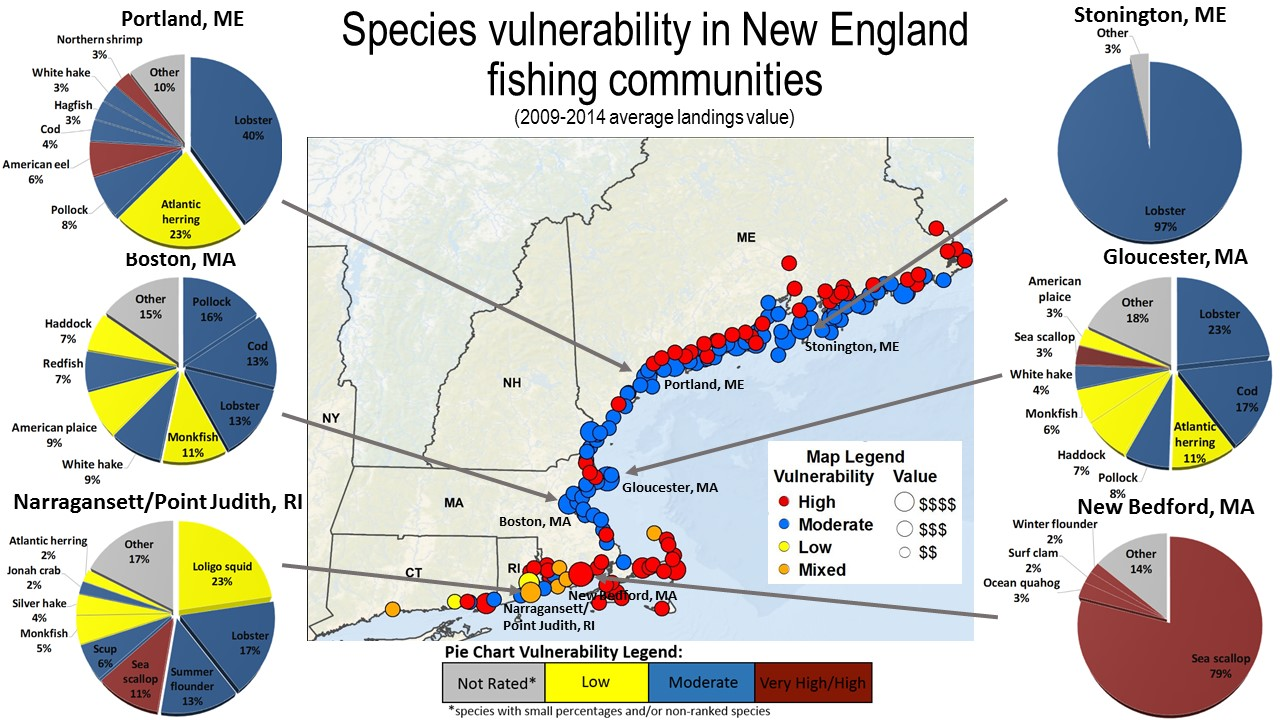
\includegraphics{C:/Users/kimberly.bastille/Desktop/tech-doc/images/Species_vulnerability_NE} 

}

\caption{Commercial species vulnerability to climate change in in New England fishing communities.}\label{fig:species-vulnerability}
\end{figure}

\chapter{Conceptual Models}\label{conceptual-models}

\textbf{Description}: Conceptual models for the New England (Georges
Bank and Gulf of Maine) and Mid-Atlantic regions of the Northeast US
Large Marine Ecosystem

\textbf{Found in}: State of the Ecosystem - Gulf of Maine \& Georges
Bank (2018,2019), State of the Ecosystem - Mid-Atlantic (2018,2019)

\textbf{Indicator category}: Synthesis of published information,
Extensive analysis; not yet published

\textbf{Contributor(s)}: Sarah Gaichas, Patricia Clay, Geret DePiper,
Gavin Fay, Michael Fogarty, Paula Fratantoni, Robert Gamble, Sean Lucey,
Charles Perretti, Patricia Pinto da Silva, Vincent Saba, Laurel Smith,
Jamie Tam, Steve Traynor, Robert Wildermuth

\textbf{Data steward}: Sarah Gaichas,
\href{mailto:sarah.gaichas@noaa.gov}{\nolinkurl{sarah.gaichas@noaa.gov}}

\textbf{Point of contact}: Sarah Gaichas,
\href{mailto:sarah.gaichas@noaa.gov}{\nolinkurl{sarah.gaichas@noaa.gov}}

\textbf{Public availability statement}: All source data aside from
confidential commercial fisheries data (relevant only to some components
of the conceptual models) are available to the public (see Data Sources
below).

\section{Methods}\label{methods-9}

Conceptual models were constructed to facilitate multidisciplinary
analysis and discussion of the linked social-ecological system for
integrated ecosystem assessment. The overall process was to first
identify the components of the model (focal groups, human activities,
environmental drivers, and objectives), and then to document criteria
for including groups and linkages and what the specific links were
between the components.

The prototype conceptual model used to design Northeast US conceptual
models for each ecosystem production unit (EPU) was designed by the
California Current IEA program. The California Current IEA developed an
\href{https://www.integratedecosystemassessment.noaa.gov/regions/california-current/cc-ecosystem-components}{overview
conceptual model for the Northern California Current Large Marine
Ecosystem (NCC)}, with models for each
\href{https://www.integratedecosystemassessment.noaa.gov/regions/california-current/cc-coastalpelagicspecies\#overview}{focal
ecosystem component} that detailed the
\href{https://www.integratedecosystemassessment.noaa.gov/regions/california-current/cc-coastalpelagicspecies\#ecologicalinteractions}{ecological},
\href{https://www.integratedecosystemassessment.noaa.gov/regions/california-current/cc-coastalpelagicspecies\#environmentalDrivers}{environmental},
and
\href{https://www.integratedecosystemassessment.noaa.gov/regions/california-current/cc-coastalpelagicspecies\#humanActivities}{human
system} linkages. Another set of conceptual models outlined
\href{https://www.integratedecosystemassessment.noaa.gov/regions/california-current/cc-habitat}{habitat}
linkages.

An inital conceptual model for Georges Bank and the Gulf of Maine was
outlined at the 2015 ICES WGNARS meeting. It specified four categories:
Large scale drivers, focal ecosystem components, human activities, and
human well being. Strategic management objectives were included in the
conceptual model, which had not been done in the NCC. Focal ecosystem
components were defined as aggregate species groups that had associated
US management objectives (outlined within WGNARS for IEAs, see DePiper
et al. (\protect\hyperlink{ref-depiper_operationalizing_2017}{2017})):
groundfish, forage fish, fished invertebrates, living habitat, and
protected species. These categories roughly align with Fishery Managment
Plans (FMPs) for the New England Fishery Management Council. The
Mid-Atlantic conceptual model was developed along similar lines, but the
focal groups included demersals, forage fish, squids, medium pelagics,
clams/quahogs, and protected species to better align with the Mid
Atlantic Council's FMPs.

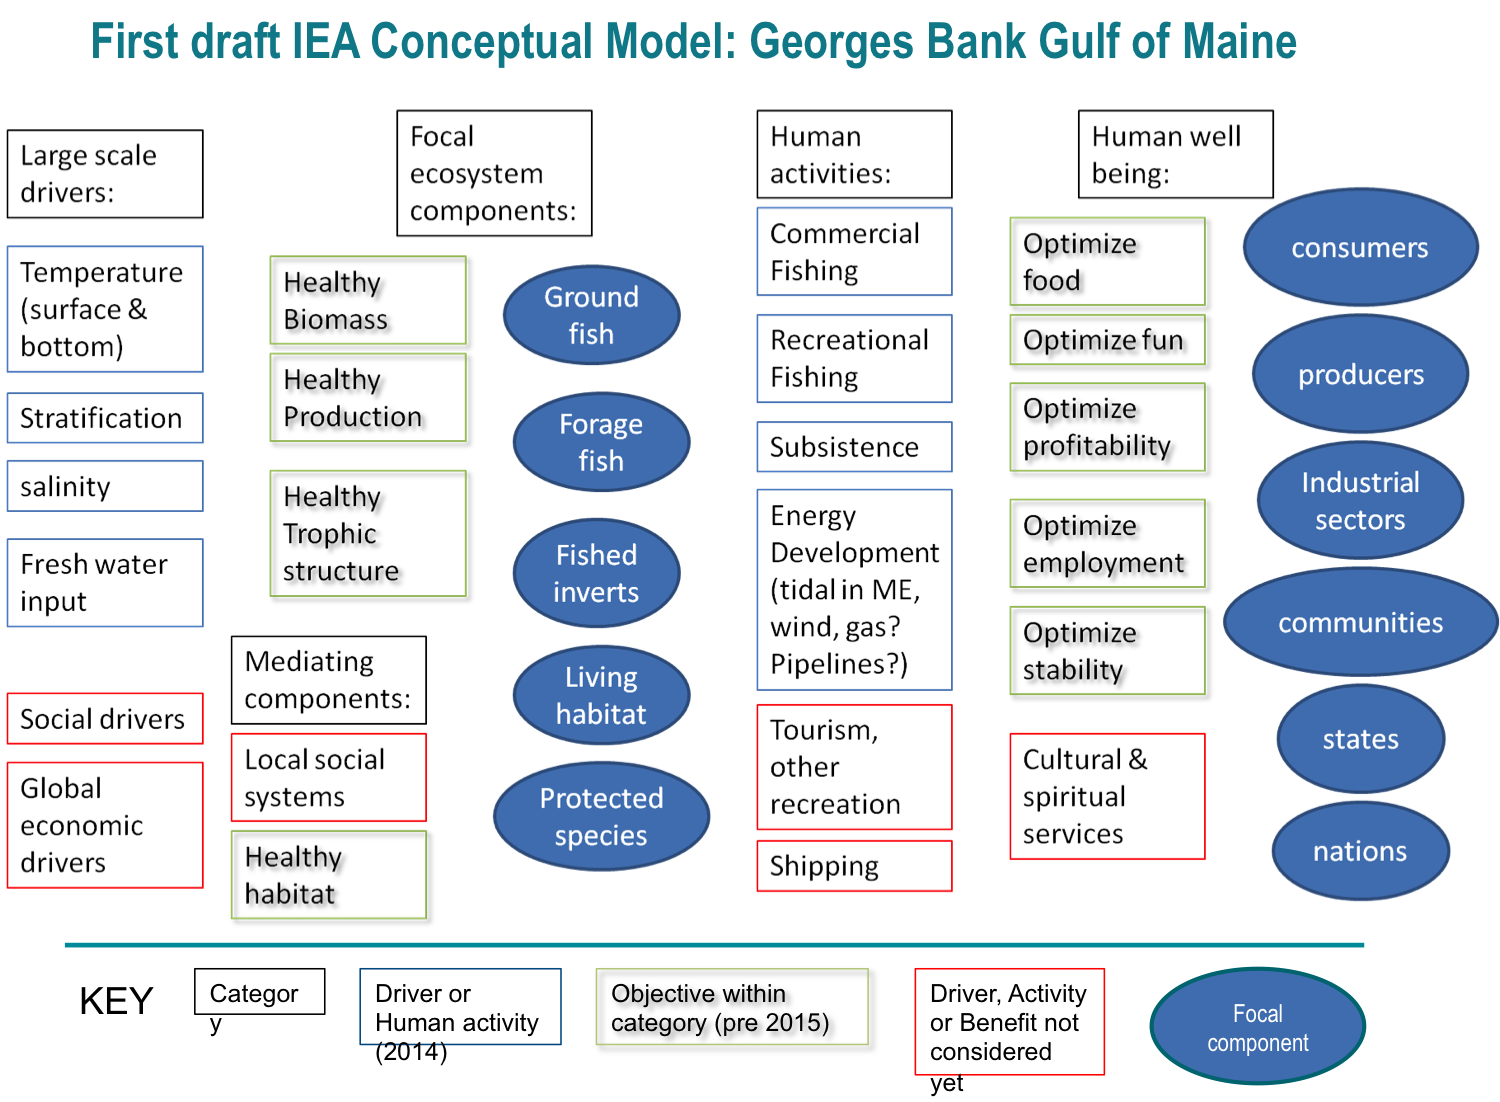
\includegraphics[width=20.83in]{C:/Users/kimberly.bastille/Desktop/tech-doc/images/GBGOMconceptual1}

After the initial draft model was outlined, working groups were formed
to develop three submodels following the CCE example: ecological,
environmental, and human dimensions. The general approach was to specify
what was being included in each group, what relationship was represented
by a link between groups, what threshold of the relationship was used to
determine whether a relationship was significant enough to be included
(we did not want to model everything), the direction and uncertainty of
the link, and documentation supporting the link between groups. This
information was recorded in a
\href{https://comet.nefsc.noaa.gov/erddap/tabledap/concept_model_2018.html}{spreadsheet}.
Submodels were then merged together by common components using the
``merge'' function in the (currently unavailable) desktop version of
Mental Modeler (\url{http://www.mentalmodeler.org/\#home}; Gray et al.
(\protect\hyperlink{ref-gray_mental_2013}{2013})). The process was
applied to Georges Bank (GB), the Gulf of Maine (GOM), and the
Mid-Atlantic Bight (MAB) \protect\hyperlink{epu}{Ecological Production
Units}.

\subsection{Data sources}\label{data-sources-9}

\subsubsection{Ecological submodels}\label{ecological-submodels}

Published food web (EMAX) models for each subregion (J.S. Link et al.
\protect\hyperlink{ref-link_documentation_2006}{2006}; Link et al.
\protect\hyperlink{ref-link_northeast_2008}{2008}), food habits data
collected by NEFSC trawl surveys (Smith and Link
\protect\hyperlink{ref-smith_trophic_2010}{2010}), and other literature
sources (Smith et al.
\protect\hyperlink{ref-smith_consumption_2015}{2015}) were consulted.
Expert judgement was also used to adjust historical information to
current conditions, and to include broad habitat linkages to Focal
groups.

\subsubsection{Environmental submodels}\label{environmental-submodels}

Published literature on the primary environmental drivers (seasonal and
interannual) in each EPU was consulted. Sources for Georges Bank
included Backus and Bourne
(\protect\hyperlink{ref-backus_georges_1987}{1987}) and Townsend et al.
(\protect\hyperlink{ref-townsend_oceanography_2006}{2006}). Sources for
the Gulf of Maine included Smith
(\protect\hyperlink{ref-smith_mean_1983}{1983}), Smith et al.
(\protect\hyperlink{ref-smith_interannual_2001}{2001}), Mupparapu and
Brown (\protect\hyperlink{ref-mupparapu_role_2002}{2002}), Townsend et
al. (\protect\hyperlink{ref-townsend_oceanography_2006}{2006}), Smith et
al. (\protect\hyperlink{ref-smith_regime_2012}{2012}), and Mountain
(\protect\hyperlink{ref-mountain_labrador_2012}{2012}).\\
Sources for the Mid Atlantic Bight included Houghton et al.
(\protect\hyperlink{ref-houghton_middle_1982}{1982}), Beardsley et al.
(\protect\hyperlink{ref-beardsley_nantucket_1985}{1985}), Lentz
(\protect\hyperlink{ref-lentz_climatology_2003}{2003}), Mountain
(\protect\hyperlink{ref-mountain_variability_2003}{2003}), Glenn et al.
(\protect\hyperlink{ref-glenn_biogeochemical_2004}{2004}), Sullivan,
Cowen, and Steves
(\protect\hyperlink{ref-sullivan_evidence_2005}{2005}), Castelao et al.
(\protect\hyperlink{ref-castelao_seasonal_2008}{2008}), Shearman and
Lentz (\protect\hyperlink{ref-shearman_long-term_2009}{2009}), Castelao,
Glenn, and Schofield
(\protect\hyperlink{ref-castelao_temperature_2010}{2010}), Gong, Kohut,
and Glenn (\protect\hyperlink{ref-gong_seasonal_2010}{2010}),
Gawarkiewicz et al.
(\protect\hyperlink{ref-gawarkiewicz_direct_2012}{2012}), Forsyth,
Andres, and Gawarkiewicz
(\protect\hyperlink{ref-forsyth_recent_2015}{2015}), Fratantoni,
Holzwarth-Davis, and Taylor
(\protect\hyperlink{ref-fratantoni_description_2015}{2015}), Zhang and
Gawarkiewicz (\protect\hyperlink{ref-zhang_dynamics_2015}{2015}),
Miller, Hare, and Alade
(\protect\hyperlink{ref-miller_state-space_2016}{2016}), and Lentz
(\protect\hyperlink{ref-lentz_seasonal_2017}{2017}).

\subsubsection{Human dimensions
submodels}\label{human-dimensions-submodels}

Fishery catch and bycatch information was drawn from multiple regional
datasets, incuding the Greater Atlantic Regional Office Vessel Trip
Reports \& Commercial Fisheries Dealer databases, Northeast Fishery
Observer Program \& Northeast At-Sea Monitoring databases, Northeast
Fishery Science Center Social Sciences Branch cost survey, and the
Marine Recreational Informational Program database. Further synthesis of
human welfare derived from fisheries was drawn from Färe, Kirkley, and
Walden (\protect\hyperlink{ref-fare_adjusting_2006}{2006}), Walden et
al. (\protect\hyperlink{ref-walden_productivity_2012}{2012}), Lee and
Thunberg (\protect\hyperlink{ref-lee_inverse_2013}{2013}), Lee
(\protect\hyperlink{ref-lee_hedonic_2014}{2014}), and Lee, Steinback,
and Wallmo (\protect\hyperlink{ref-lee_applying_2017}{2017}). Bycatch of
protected species was taken from Waring et al.
(\protect\hyperlink{ref-waring_us_2015}{2015}), with additional insights
from Bisack and Magnusson
(\protect\hyperlink{ref-bisack_measuring_2014}{2014}). The top 3
linkages were drawn for each node. For example, the top 3 recreational
species for the Mid-Atlantic were used to draw linkages between the
recreational fishery and species focal groups. A similar approach was
used for relevant commercial fisheries in each region.

Habitat-fishery linkages were drawn from unpublished reports, including:

\begin{enumerate}
\def\labelenumi{\arabic{enumi}.}
\item
  Mid-Atlantic Fishery Management Council. 2016.
  \href{http://www.mafmc.org/actions/msb-am16}{Amendment 16} to the
  Atlantic Mackerel, Squid, and Butterfish Fishery Management Plan:
  Measures to protect deep sea corals from Impacts of Fishing Gear.
  Environmental Assessment, Regulatory Impact Review, and Initial
  Regulatory Flexibility Analysis. Dover, DE. August, 2016.
\item
  NOAA. 2016. Deep sea coral research and technology program 2016 Report
  to Congress.
  \url{http://www.habitat.noaa.gov/protection/corals/deepseacorals.html}
  retrieved February 8, 2017.
\item
  New England Fishery Management Council. 2016. Habitat Omnibus Deep-Sea
  Coral Amendment: Draft.
  \url{http://www.nefmc.org/library/omnibus-deep-sea-coral-amendment}
  Retrieved Feb 8, 2017.
\item
  Bachman et al. 2011. The Swept Area Seabed Impact (SASI) Model: A Tool
  for Analyzing the Effects of Fishing on Essential Fish Habitat. New
  England Fisheries Management Council Report. Newburyport, MA.
\end{enumerate}

Tourism and habitat linkages were drawn from unpublished reports,
including:

\begin{enumerate}
\def\labelenumi{\arabic{enumi}.}
\item
  \url{http://neers.org/RESOURCES/Bibliographies.html}
\item
  Great Bay (GoM) resources
  \url{http://greatbay.org/about/publications.htm}
\item
  Meaney, C.R. and C. Demarest. 2006. Coastal Polution and New England
  Fisheries. Report for the New England Fisheries Management Council.
  Newburyport, MA.
\item
  List of valuation studies, by subregion and/or state, can be found at
  \url{http://www.oceaneconomics.org/nonmarket/valestim.asp}.
\end{enumerate}

Published literature on human activities in each EPU was consulted.

Sources for protected species and tourism links included Hoagland and
Meeks (\protect\hyperlink{ref-hoagland_demand_2000}{2000}) and Lee
(\protect\hyperlink{ref-lee_economic_2010}{2010}).

Sources for links between environmental drivers and human activities
included Adams (\protect\hyperlink{ref-adams_uncertainty_1973}{1973}),
Matzarakis and Freitas
(\protect\hyperlink{ref-matzarakis_proceedings_2001}{2001}), Scott,
McBoyle, and Schwartzentruber
(\protect\hyperlink{ref-scott_climate_2004}{2004}), Hess, Malilay, and
Parkinson (\protect\hyperlink{ref-hess_climate_2008}{2008}), Colburn and
Jepson (\protect\hyperlink{ref-colburn_social_2012}{2012}), Jepson and
Colburn (\protect\hyperlink{ref-jepson_development_2013}{2013}), and
Colburn et al. (\protect\hyperlink{ref-colburn_indicators_2016}{2016}).

Sources for cultural practices and attachments links included Pauly
(\protect\hyperlink{ref-pauly_putting_1997}{1997}), McGoodwin
(\protect\hyperlink{ref-mcgoodwin_understanding_2001}{2001}), St Martin
(\protect\hyperlink{ref-st_martin_making_2001}{2001}), Norris-Raynbird
(\protect\hyperlink{ref-norris-raynbird_for_2004}{2004}), Pollnac et al.
(\protect\hyperlink{ref-pollnac_toward_2006}{2006}), Clay and Olson
(\protect\hyperlink{ref-clay_defining_2007}{2007}), Clay and Olson
(\protect\hyperlink{ref-clay_definingfishing_2008}{2008}), Everett and
Aitchison (\protect\hyperlink{ref-everett_role_2008}{2008}), Donkersloot
(\protect\hyperlink{ref-donkersloot_politics_2010}{2010}), Lord
(\protect\hyperlink{ref-lord_understanding_2011}{2011}), Halpern et al.
(\protect\hyperlink{ref-halpern_index_2012}{2012}), Wynveen, Kyle, and
Sutton (\protect\hyperlink{ref-wynveen_natural_2012}{2012}),
Cortes-Vazquez and Zedalis
(\protect\hyperlink{ref-cortes-vazquez_identity_2013}{2013}), Koehn,
Reineman, and Kittinger
(\protect\hyperlink{ref-koehn_progress_2013}{2013}), Potschin and
Haines-Young (\protect\hyperlink{ref-potschin_landscapes_2013}{2013}),
Reed et al. (\protect\hyperlink{ref-reed_beyond_2013}{2013}), Urquhart
and Acott (\protect\hyperlink{ref-urquhart_constructing_2013}{2013}),
Blasiak et al. (\protect\hyperlink{ref-blasiak_paradigms_2014}{2014}),
Klain, Satterfield, and Chan
(\protect\hyperlink{ref-klain_what_2014}{2014}), Poe, Norman, and Levin
(\protect\hyperlink{ref-poe_cultural_2014}{2014}), Brown
(\protect\hyperlink{ref-brown_we_2015}{2015}), Donatuto and Poe
(\protect\hyperlink{ref-donatuto_evaluating_2015}{2015}), Khakzad and
Griffith (\protect\hyperlink{ref-khakzad_role_2016}{2016}), Oberg et al.
(\protect\hyperlink{ref-oberg_surviving_2016}{2016}), and Seara, Clay,
and Colburn (\protect\hyperlink{ref-seara_perceived_2016}{2016}).

\subsection{Data extraction}\label{data-extraction-8}

\subsubsection{Ecological submodels}\label{ecological-submodels-1}

``Data'' included model estimated quantities to determine whether
inclusion thresholds were met for each potential link in the conceptual
model. A matrix with diet composition for each modeled group is an input
to the food web model. A matrix of mortalities caused by each predator
and fishery on each modeled group is a direct ouput of a food web model
(e.g.~Ecopath). Food web model biomasss flows between species,
fisheries, and detritus were summarized using algorithms implemented in
visual basic by Kerim Aydin, NOAA NMFS Alaska Fisheries Science Center.
Because EMAX model groups were aggregated across species, selected diet
compositions for individual species were taken from the NEFSC food
habits database using the FEAST program for selected species (example
query below). These diet queries were consulted as supplemental
information.

Example FEAST sql script for Cod weighted diet on Georges Bank. Queries
for different species are standardized by the FEAST application and
would differ only in the svspp code.

\begin{Shaded}
\begin{Highlighting}[]
\KeywordTok{Select}\NormalTok{ svspp,}\DataTypeTok{year}\NormalTok{,cruise6,stratum,station,catsex,pdid,pdgutw,pdlen,pdwgt,perpyw,pyamtw,COLLCAT,numlen,pyamtv  }\KeywordTok{from}\NormalTok{ fhdbs.allfh_feast }\KeywordTok{where}\NormalTok{ pynam <> }\StringTok{'BLOWN'} \KeywordTok{and}\NormalTok{ pynam <> }\StringTok{'PRESERVED'} \KeywordTok{and}\NormalTok{ pynam <> }\StringTok{' '} \KeywordTok{and}\NormalTok{ svspp=}\StringTok{'073'} \KeywordTok{and} \DataTypeTok{YEAR} \KeywordTok{BETWEEN} \StringTok{'1973'} \KeywordTok{AND} \StringTok{'2016'} \KeywordTok{and}\NormalTok{ GEOAREA=}\StringTok{'GB'} \KeywordTok{order} \KeywordTok{by}\NormalTok{ svspp,}\DataTypeTok{year}\NormalTok{,cruise6,stratum,station,pdid,COLLCAT}
\KeywordTok{Select} \KeywordTok{distinct}\NormalTok{ svspp,}\DataTypeTok{year}\NormalTok{,cruise6,stratum,station }\KeywordTok{from}\NormalTok{ fhdbs.allfh_feast }\KeywordTok{where}\NormalTok{ pynam <> }\StringTok{'BLOWN'} \KeywordTok{and}\NormalTok{ pynam <> }\StringTok{'PRESERVED'} \KeywordTok{and}\NormalTok{ pynam <> }\StringTok{' '} \KeywordTok{and}\NormalTok{ svspp=}\StringTok{'073'} \KeywordTok{and} \DataTypeTok{YEAR} \KeywordTok{BETWEEN} \StringTok{'1973'} \KeywordTok{AND} \StringTok{'2016'} \KeywordTok{and}\NormalTok{ GEOAREA=}\StringTok{'GB'} \KeywordTok{order} \KeywordTok{by}\NormalTok{ svspp,}\DataTypeTok{year}\NormalTok{,cruise6,stratum,station}
\KeywordTok{Select} \KeywordTok{distinct}\NormalTok{ svspp,}\DataTypeTok{year}\NormalTok{,cruise6,stratum,station,catsex,catnum }\KeywordTok{from}\NormalTok{ fhdbs.allfh_feast }\KeywordTok{where}\NormalTok{ pynam <> }\StringTok{'BLOWN'} \KeywordTok{and}\NormalTok{ pynam <> }\StringTok{'PRESERVED'} \KeywordTok{and}\NormalTok{ pynam <> }\StringTok{' '} \KeywordTok{and}\NormalTok{ svspp=}\StringTok{'073'} \KeywordTok{and} \DataTypeTok{YEAR} \KeywordTok{BETWEEN} \StringTok{'1973'} \KeywordTok{AND} \StringTok{'2016'} \KeywordTok{and}\NormalTok{ GEOAREA=}\StringTok{'GB'} \KeywordTok{order} \KeywordTok{by}\NormalTok{ svspp,}\DataTypeTok{year}\NormalTok{,cruise6,stratum,station}
\KeywordTok{Select} \KeywordTok{distinct}\NormalTok{ COLLCAT }\KeywordTok{from}\NormalTok{ fhdbs.allfh_feast }\KeywordTok{where}\NormalTok{ pynam <> }\StringTok{'BLOWN'} \KeywordTok{and}\NormalTok{ pynam <> }\StringTok{'PRESERVED'} \KeywordTok{and}\NormalTok{ pynam <> }\StringTok{' '} \KeywordTok{and}\NormalTok{ svspp=}\StringTok{'073'} \KeywordTok{and} \DataTypeTok{YEAR} \KeywordTok{BETWEEN} \StringTok{'1973'} \KeywordTok{AND} \StringTok{'2016'} \KeywordTok{and}\NormalTok{ GEOAREA=}\StringTok{'GB'} \KeywordTok{order} \KeywordTok{by}\NormalTok{ COLLCAT}
\KeywordTok{Select} \KeywordTok{distinct}\NormalTok{ svspp,}\DataTypeTok{year}\NormalTok{,cruise6,stratum,station,catsex,pdid,pdlen,pdgutw,pdwgt  }\KeywordTok{from}\NormalTok{ fhdbs.allfh_feast }\KeywordTok{where}\NormalTok{ pynam <> }\StringTok{'BLOWN'} \KeywordTok{and}\NormalTok{ pynam <> }\StringTok{'PRESERVED'} \KeywordTok{and}\NormalTok{ pynam <> }\StringTok{' '} \KeywordTok{and}\NormalTok{ svspp=}\StringTok{'073'} \KeywordTok{and} \DataTypeTok{YEAR} \KeywordTok{BETWEEN} \StringTok{'1973'} \KeywordTok{AND} \StringTok{'2016'} \KeywordTok{and}\NormalTok{ GEOAREA=}\StringTok{'GB'} \KeywordTok{order} \KeywordTok{by}\NormalTok{ svspp,}\DataTypeTok{year}\NormalTok{,cruise6,stratum,station,catsex,pdid}
\KeywordTok{Select}\NormalTok{ svspp,}\DataTypeTok{year}\NormalTok{,cruise6,stratum,station,catsex,pdid,pdlen,COLLCAT,}\FunctionTok{sum}\NormalTok{(perpyw),}\FunctionTok{sum}\NormalTok{(pyamtw),}\FunctionTok{sum}\NormalTok{(pyamtv)  }\KeywordTok{from}\NormalTok{ fhdbs.allfh_feast }\KeywordTok{where}\NormalTok{ pynam <> }\StringTok{'BLOWN'} \KeywordTok{and}\NormalTok{ pynam <> }\StringTok{'PRESERVED'} \KeywordTok{and}\NormalTok{ pynam <> }\StringTok{' '} \KeywordTok{and}\NormalTok{ svspp=}\StringTok{'073'} \KeywordTok{and} \DataTypeTok{YEAR} \KeywordTok{BETWEEN} \StringTok{'1973'} \KeywordTok{AND} \StringTok{'2016'} \KeywordTok{and}\NormalTok{ GEOAREA=}\StringTok{'GB'} \KeywordTok{group} \KeywordTok{by}\NormalTok{ svspp,}\DataTypeTok{year}\NormalTok{,cruise6,stratum,station,catsex,pdid,pdlen,COLLCAT }\KeywordTok{order} \KeywordTok{by}\NormalTok{ svspp,}\DataTypeTok{year}\NormalTok{,cruise6,stratum,station,catsex,pdid,pdlen,COLLCAT}
\KeywordTok{Select}\NormalTok{ svspp,}\DataTypeTok{year}\NormalTok{,cruise6,stratum,station,COLLCAT,}\FunctionTok{sum}\NormalTok{(pyamtv) sumpvol }\KeywordTok{from}\NormalTok{ fhdbs.allfh_feast }\KeywordTok{where}\NormalTok{ pynam <> }\StringTok{'BLOWN'} \KeywordTok{and}\NormalTok{ pynam <> }\StringTok{'PRESERVED'} \KeywordTok{and}\NormalTok{ pynam <> }\StringTok{' '} \KeywordTok{and}\NormalTok{ svspp=}\StringTok{'073'} \KeywordTok{and} \DataTypeTok{YEAR} \KeywordTok{BETWEEN} \StringTok{'1973'} \KeywordTok{AND} \StringTok{'2016'} \KeywordTok{and}\NormalTok{ GEOAREA=}\StringTok{'GB'} \KeywordTok{group} \KeywordTok{by}\NormalTok{ svspp,}\DataTypeTok{year}\NormalTok{,cruise6,stratum,station,COLLCAT }\KeywordTok{order} \KeywordTok{by}\NormalTok{ svspp,}\DataTypeTok{year}\NormalTok{,cruise6,stratum,station,COLLCAT}
\KeywordTok{Select}\NormalTok{ svspp,}\DataTypeTok{year}\NormalTok{,cruise6,stratum,station, }\FunctionTok{count}\NormalTok{(}\KeywordTok{distinct}\NormalTok{ pdid) nstom  }\KeywordTok{from}\NormalTok{ fhdbs.allfh_feast }\KeywordTok{where}\NormalTok{ pynam <> }\StringTok{'BLOWN'} \KeywordTok{and}\NormalTok{ pynam <> }\StringTok{'PRESERVED'} \KeywordTok{and}\NormalTok{ pynam <> }\StringTok{' '} \KeywordTok{and}\NormalTok{ svspp=}\StringTok{'073'} \KeywordTok{and} \DataTypeTok{YEAR} \KeywordTok{BETWEEN} \StringTok{'1973'} \KeywordTok{AND} \StringTok{'2016'} \KeywordTok{and}\NormalTok{ GEOAREA=}\StringTok{'GB'} \KeywordTok{group} \KeywordTok{by}\NormalTok{ svspp,}\DataTypeTok{year}\NormalTok{,cruise6,stratum,station,catsex }\KeywordTok{order} \KeywordTok{by}\NormalTok{ svspp,}\DataTypeTok{year}\NormalTok{,cruise6,stratum,station}
\KeywordTok{Select}\NormalTok{ svspp,}\DataTypeTok{year}\NormalTok{,cruise6,stratum,station,pdlen,numlen,}\FunctionTok{count}\NormalTok{(}\KeywordTok{distinct}\NormalTok{ pdid) nstom  }\KeywordTok{from}\NormalTok{ fhdbs.allfh_feast }\KeywordTok{where}\NormalTok{ pynam <> }\StringTok{'BLOWN'} \KeywordTok{and}\NormalTok{ pynam <> }\StringTok{'PRESERVED'} \KeywordTok{and}\NormalTok{ pynam <> }\StringTok{' '} \KeywordTok{and}\NormalTok{ numlen }\KeywordTok{is} \KeywordTok{not} \KeywordTok{null} \KeywordTok{and}\NormalTok{ svspp=}\StringTok{'073'} \KeywordTok{and} \DataTypeTok{YEAR} \KeywordTok{BETWEEN} \StringTok{'1973'} \KeywordTok{AND} \StringTok{'2016'} \KeywordTok{and}\NormalTok{ GEOAREA=}\StringTok{'GB'} \KeywordTok{group} \KeywordTok{by}\NormalTok{ svspp,}\DataTypeTok{year}\NormalTok{,cruise6,stratum,station,pdlen,numlen,catsex }\KeywordTok{order} \KeywordTok{by}\NormalTok{ svspp,}\DataTypeTok{year}\NormalTok{,cruise6,stratum,station,pdlen}
\KeywordTok{Select}\NormalTok{ svspp,}\DataTypeTok{year}\NormalTok{,cruise6,stratum,station,pdlen,COLLCAT,}\FunctionTok{sum}\NormalTok{(pyamtv) sumpvol  }\KeywordTok{from}\NormalTok{ fhdbs.allfh_feast }\KeywordTok{where}\NormalTok{ pynam <> }\StringTok{'BLOWN'} \KeywordTok{and}\NormalTok{ pynam <> }\StringTok{'PRESERVED'} \KeywordTok{and}\NormalTok{ pynam <> }\StringTok{' '} \KeywordTok{and}\NormalTok{ svspp=}\StringTok{'073'} \KeywordTok{and} \DataTypeTok{YEAR} \KeywordTok{BETWEEN} \StringTok{'1973'} \KeywordTok{AND} \StringTok{'2016'} \KeywordTok{and}\NormalTok{ GEOAREA=}\StringTok{'GB'} \KeywordTok{group} \KeywordTok{by}\NormalTok{ svspp,}\DataTypeTok{year}\NormalTok{,cruise6,stratum,station,pdlen,COLLCAT }\KeywordTok{order} \KeywordTok{by}\NormalTok{ svspp,}\DataTypeTok{year}\NormalTok{,cruise6,stratum,station,pdlen,COLLCAT}
\KeywordTok{Select} \KeywordTok{distinct}\NormalTok{ svspp,}\DataTypeTok{year}\NormalTok{,cruise6,stratum,station,pdid,pdlen }\KeywordTok{from}\NormalTok{ fhdbs.allfh_feast }\KeywordTok{where}\NormalTok{ pynam <> }\StringTok{'BLOWN'} \KeywordTok{and}\NormalTok{ pynam <> }\StringTok{'PRESERVED'} \KeywordTok{and}\NormalTok{ pynam <> }\StringTok{' '} \KeywordTok{and}\NormalTok{ numlen }\KeywordTok{is} \KeywordTok{null} \KeywordTok{and}\NormalTok{ svspp=}\StringTok{'073'} \KeywordTok{and} \DataTypeTok{YEAR} \KeywordTok{BETWEEN} \StringTok{'1973'} \KeywordTok{AND} \StringTok{'2016'} \KeywordTok{and}\NormalTok{ GEOAREA=}\StringTok{'GB'}
\KeywordTok{Select} \KeywordTok{distinct} \DataTypeTok{year}\NormalTok{,cruise6,stratum,station,beglat,beglon  }\KeywordTok{from}\NormalTok{ fhdbs.allfh_feast }\KeywordTok{where}\NormalTok{ pynam <> }\StringTok{'BLOWN'} \KeywordTok{and}\NormalTok{ pynam <> }\StringTok{'PRESERVED'} \KeywordTok{and}\NormalTok{ pynam <> }\StringTok{' '} \KeywordTok{and}\NormalTok{ svspp=}\StringTok{'073'} \KeywordTok{and} \DataTypeTok{YEAR} \KeywordTok{BETWEEN} \StringTok{'1973'} \KeywordTok{AND} \StringTok{'2016'} \KeywordTok{and}\NormalTok{ GEOAREA=}\StringTok{'GB'} \KeywordTok{order} \KeywordTok{by} \DataTypeTok{year}\NormalTok{,cruise6,stratum,station}
\end{Highlighting}
\end{Shaded}

\subsubsection{Environmental submodels}\label{environmental-submodels-1}

Information was synthesized entirely from published sources and expert
knowledge; no additional data extraction was completed for the
environmental submodels.

\subsubsection{Human dimensions
submodels}\label{human-dimensions-submodels-1}

Recreational fisheries data were extracted from the 2010-2014 MRIP
datasets. Original data can be found
\href{data/top10_prim1_common_mode.xlsx}{here} for each region (New
England or Mid-Atlantic as defined by states).

Commercial fishing data was developed as part of the State of the
Ecosystem Report, including revenue and food production estimates, with
data extraction metodology discussed in the relevant sections of the
technical document. In addition, the Northeast Regional Input/Output
Model (Steinback and Thunberg
\protect\hyperlink{ref-steinback_scott_northeast_2006}{2006}) was used
as the basis for the strength of the employment linkages.

\subsection{Data analysis}\label{data-analysis-8}

\subsubsection{Ecological submodels}\label{ecological-submodels-2}

Aggregated diet and mortality information was examined to determine the
type of link, direction of link, and which links between which groups
should be inclded in the conceptual models. Two types of ecological
links were defined using food web models: prey links and
predation/fishing mortality links. Prey links resulted in positve links
between the prey group and the focal group, while predation/fishing
mortality links resulted in negative links to the focal group to
represent energy flows. The intent was to include only the most
important linkages between focal groups and with other groups supporting
or causing mortality on focal species groups. Therefore, threshold
levels of diet and mortality were established (based on those that would
select the top 1-3 prey and predators of each focal group): 10\% to
include a link (or add a linked group) in the model and 20\% to include
as a strong link. A Primary Production group was included in each model
and linked to pelagic habitat to allow environmental effects on habitat
to be connected to the ecologial submodel. Uncertainty for the inclusion
of each link and for the magnitude of each link was qualitatively
assessed and noted in the
\href{https://comet.nefsc.noaa.gov/erddap/tabledap/concept_model_2018.html}{spreadsheet}.

Four habitat categories (Pelagic, Seafloor and Demersal, Nearshore, and
Freshwater and Estuarine) were included in ecological submodels as
placeholders to be developed further along with habitat-specific
research. Expert opinion was used to include the strongest links between
each habitat type and each Focal group (noting that across species and
life stages, members of these aggregate groups likely occupy many if not
all of the habitat types). Link direction and strength were not
specified. Environmental drivers were designed to link to habitats,
rather than directly to Focal groups, to represent each habitat's
important mediation function.

EMAX model groups were aggregated to focal groups for the Georges Bank
(GB), Gulf of Maine (GOM) and Mid-Atlantic Bight (MAB) conceptual models
according to Table \ref{tab:groups}. ``Linked groups'' directly support
or impact the Focal groups as described above.

\begin{table}

\caption{\label{tab:groups}Relationship between food web model groups and conceptual model focal groups}
\centering
\begin{tabular}[t]{l|l|l|l|l}
\hline
Group Type & Region & Conceptual model group & EMAX group(s) & Notes\\
\hline
Focal & GB & Commercial Fishery & Fishery & \\
\hline
Focal & GB & Fished Inverts & Megabenthos filterers & \\
\hline
Focal & GB & Forage Fish & Sum of Small pelagics--commercial, other, anadromous, and squids & \\
\hline
Focal & GB & Groundfish & Sum of Demersals--omnivores, benthivores, and piscivores & \\
\hline
Focal & GB & Protected Species & Sum of Baleen Whales, Odontocetes, and Seabirds & Pinnipeds not included in GB EMAX\\
\hline
Linked & GB & Benthos & Sum of Macrobenthos—polychaetes, crustaceans, molluscs, other and Megabenthos—other & \\
\hline
Linked & GB & Copepods and Micronecton & Sum of Copepods--small and large, and Micronekton & \\
\hline
Linked & GB & Detritus and Bacteria & Sum of Bacteria and Detritus-POC & \\
\hline
Linked & GB & Gelatinous zooplankton & Gelatinous zooplankton & \\
\hline
Linked & GB & Primary Production & Phytoplankton-Primary production & \\
\hline
Focal & GOM & Commercial Fishery & Fishery & \\
\hline
Focal & GOM & Fished Inverts & Megabenthos filterers & \\
\hline
Focal & GOM & Forage Fish & Sum of Small pelagics--commercial, other, anadromous, and squids & \\
\hline
Focal & GOM & Groundfish & Sum of Demersals--omnivores, benthivores, and piscivores & \\
\hline
Focal & GOM & Protected Species & Sum of Baleen Whales, Odontocetes, Pinnipeds, and Seabirds & \\
\hline
Linked & GOM & Benthos & Sum of Macrobenthos—polychaetes, crustaceans, molluscs, other and Megabenthos—other & \\
\hline
Linked & GOM & Copepods and Micronecton & Sum of Copepods--small and large, and Micronekton & \\
\hline
Linked & GOM & Detritus and Bacteria & Sum of Bacteria and Detritus-POC & \\
\hline
Linked & GOM & Gelatinous zooplankton & Gelatinous zooplankton & \\
\hline
Linked & GOM & Primary Production & Phytoplankton-Primary production & \\
\hline
Focal & MAB & Clams Quahogs & Megabenthos filterers & \\
\hline
Focal & MAB & Commercial Fishery & Fishery & \\
\hline
Focal & MAB & Demerals & Sum of Demersals--omnivores, benthivores, and piscivores & \\
\hline
Focal & MAB & Forage Fish & Sum of Small pelagics--commercial, other, and anadromous & \\
\hline
Focal & MAB & Medium Pelagics & Medium pelagics & \\
\hline
Focal & MAB & Protected Species & Sum of Baleen whales and Odontocetes & Seabirds not included in MAB EMAX\\
\hline
Focal & MAB & Squids & Small pelagics--squids & \\
\hline
Linked & MAB & Benthos & Sum of Macrobenthos—polychaetes, crustaceans, molluscs, other & \\
\hline
Linked & MAB & Copepods and Micronecton & Sum of Copepods--small and large, and Micronekton & \\
\hline
Linked & MAB & Detritus and Bacteria & Sum of Bacteria and Detritus-POC & \\
\hline
Linked & MAB & Gelatinous zooplankton & Gelatinous zooplankton & \\
\hline
Linked & MAB & Primary Production & Phytoplankton-Primary production & \\
\hline
Linked & MAB & Sharks & Sum of Sharks—pelagic and coastal & \\
\hline
\end{tabular}
\end{table}

Ecological submodels were constructed and visualized in Mental Modeler
(Fig. \ref{fig:draftGOMeco}). Here, we show only the Gulf of Maine
submodels as examples.

\begin{figure}
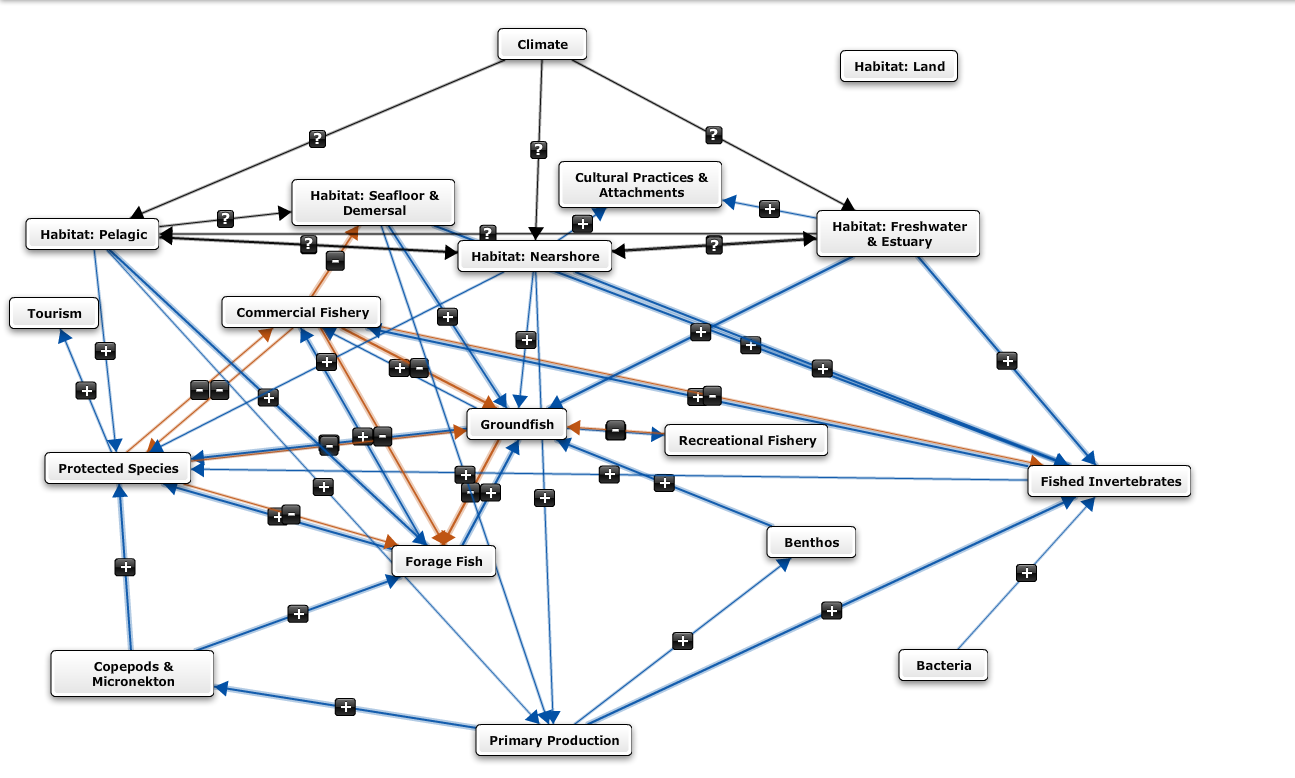
\includegraphics[width=17.99in]{C:/Users/kimberly.bastille/Desktop/tech-doc/images/MM_GoM_Ecological} \caption{Gulf of Maine Ecological submodel}\label{fig:draftGOMeco}
\end{figure}

\subsubsection{Environmental submodels}\label{environmental-submodels-2}

Environmental submodels were designed to link key oceanographic
processes in each ecosystem production unit to the four general habitat
categories (Pelagic, Seafloor and Demersal, Nearshore, and Freshwater
and Estuarine) with emphasis on the most important physical processes in
each ecosystem based on expert knowledge as supported by literature
review. The basis of each submodel were environmental variables
observable at management-relevant scales as identified by
\href{http://ices.dk/sites/pub/Publication\%20Reports/Expert\%20Group\%20Report/SSGRSP/2014/WGNARS14.pdf}{WGNARS}:
Surface and Bottom Water Temperature and Salinity, Freshwater Input, and
Stratification (as well as sea ice timing and cover, which is not
relevant to the northeast US shelf). Key drivers changing these
observable variables and thus structuring habitat dynamics in each
\protect\hyperlink{epu}{Ecological Production Units} were added to the
model using expert consensus.

Environmental submodels were initially constructed and visualized in
Mental Modeler (Fig. \ref{fig:draftGOMenv}).

\begin{figure}
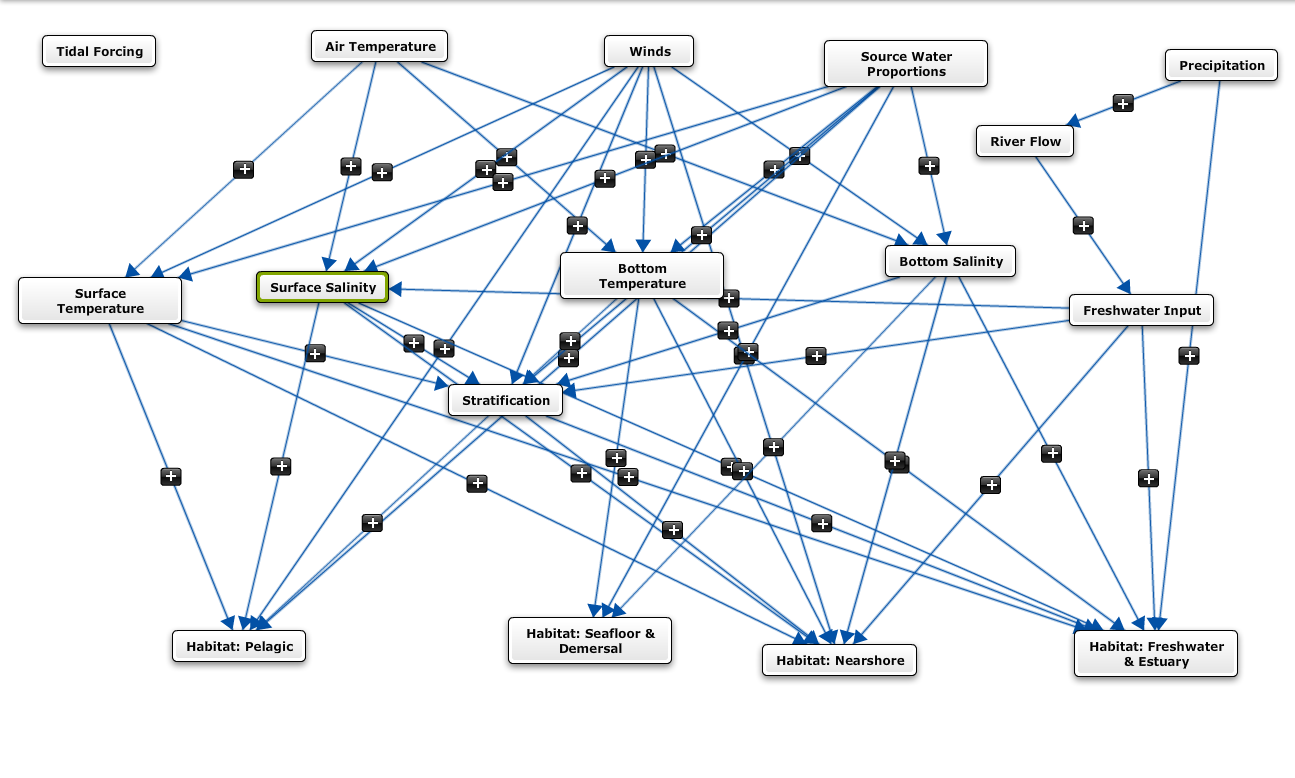
\includegraphics[width=17.99in]{C:/Users/kimberly.bastille/Desktop/tech-doc/images/MM_GoM_Climate} \caption{Gulf of Maine Environmental submodel}\label{fig:draftGOMenv}
\end{figure}

\subsubsection{Human dimensions
submodels}\label{human-dimensions-submodels-2}

The top 3 species from each mode of recreational fishing (shoreside,
private boat, party/charter) were used to assess the potential for
missing links between the recreational fishing activity and biological
focal components. Given the predominance of Mid-Atlantic groundfish in
recreational fishing off New England (summer flounder, bluefish, striped
bass), a Mid-Atlantic groundfish focal component was added to the
Georges Bank EPU model. The magnitude of benefits generated from
recreational fishing was scaled to reflect expert knowledge of target
species, coupled with the MRIP data highlighted above. Scales were held
consistent across the focal components within recreational fishing.

No additional biological focal components were added to the commercial
fishing activity, beyond what was developed in the ecological submodel.
Benefits derived from commercial fishing were scaled to be consistent
with the State of the Ecosystem revenue estimates, as modulated by
expert knowledge and additional data sources. For example,the percentage
of landings sold as food was used to map fishing activity to the
commercial fishery food production objective, and the Northeast Regional
Input/Output Model (Steinback and Thunberg
\protect\hyperlink{ref-steinback_scott_northeast_2006}{2006}) was used
to define the strength of the employment linkages. For profitability,
expert knowledge was used to reweight revenue landings, based on
ancillary cost data available (Das, Chhandita
\protect\hyperlink{ref-das_chhandita_northeast_2013}{2013}; Das,
Chhandita \protect\hyperlink{ref-das_chhandita_overview_2014}{2014}).
Human activities and objectives for the conceptual sub model are defined
in DePiper et al.
(\protect\hyperlink{ref-depiper_operationalizing_2017}{2017}). As shown
in Figure \ref{fig:draftGOMhuman}, human dimensions submodels were also
initially constructed and visualized in Mental Modeler.

\begin{figure}
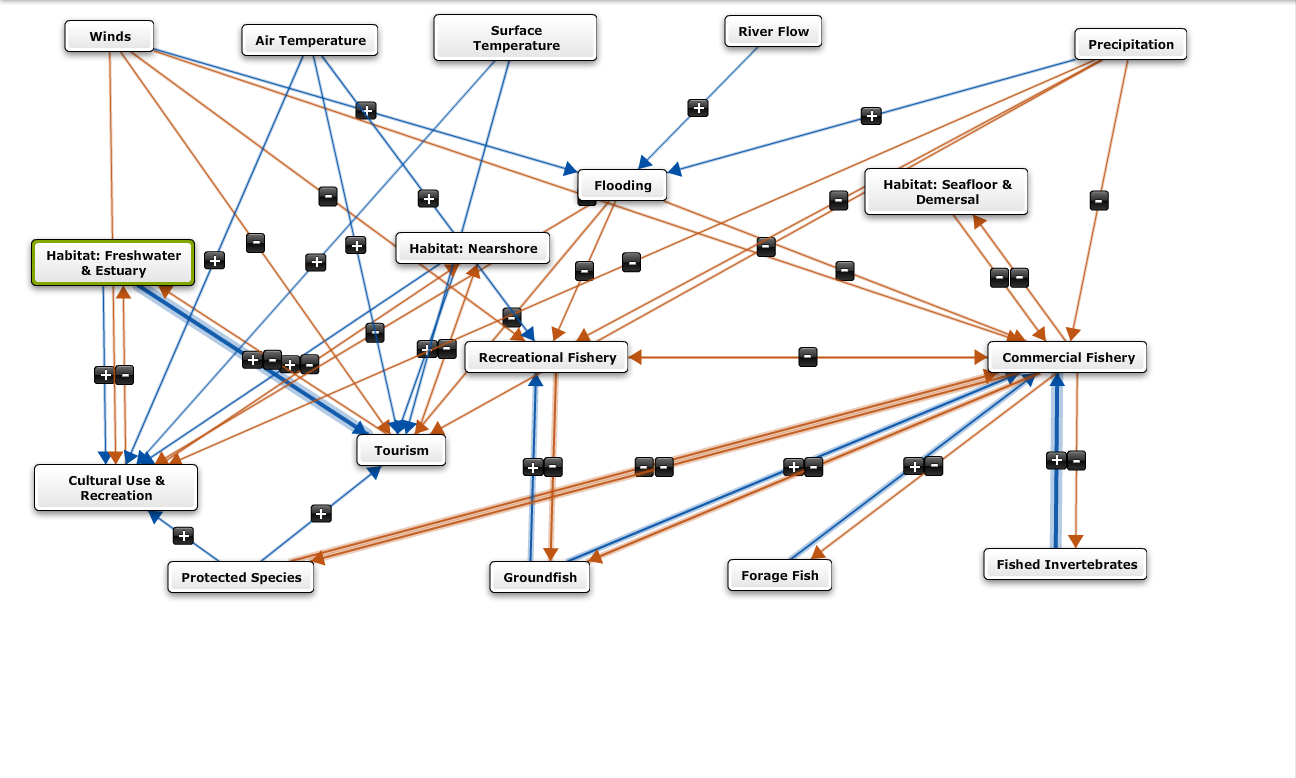
\includegraphics[width=18in]{C:/Users/kimberly.bastille/Desktop/tech-doc/images/MM_GoM_Human_Connections} \caption{Gulf of Maine Human dimensions submodel}\label{fig:draftGOMhuman}
\end{figure}

\subsubsection{Merged models}\label{merged-models}

All links and groups from each submodel were preserved in the full
merged model for each system. Mental modeler was used to merge the
submodels. Full models were then re-drawn in Dia
(\url{http://dia-installer.de/}) with color codes for each model
component type for improved readability. Examples for each system are
below.

\begin{figure}
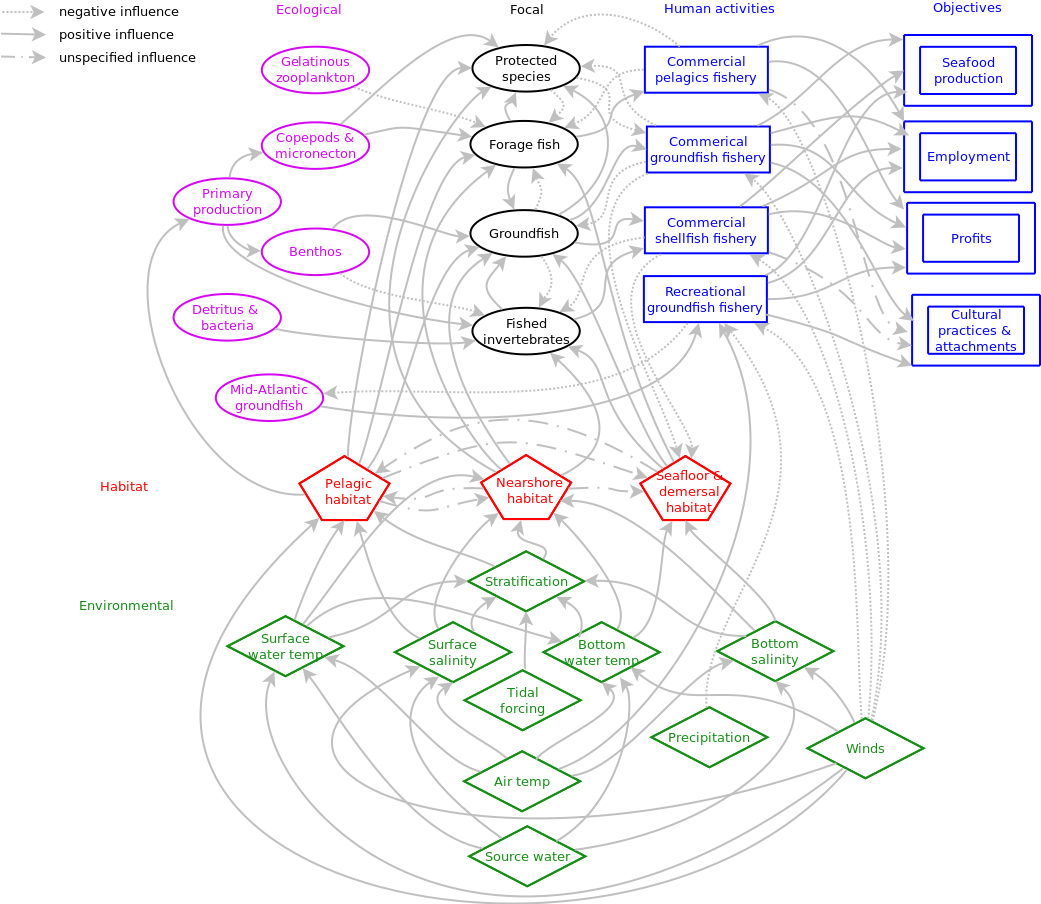
\includegraphics[width=14.46in]{C:/Users/kimberly.bastille/Desktop/tech-doc/images/GBoverview5} \caption{Georges Bank conceptual model}\label{fig:diaGB}
\end{figure}

\begin{figure}
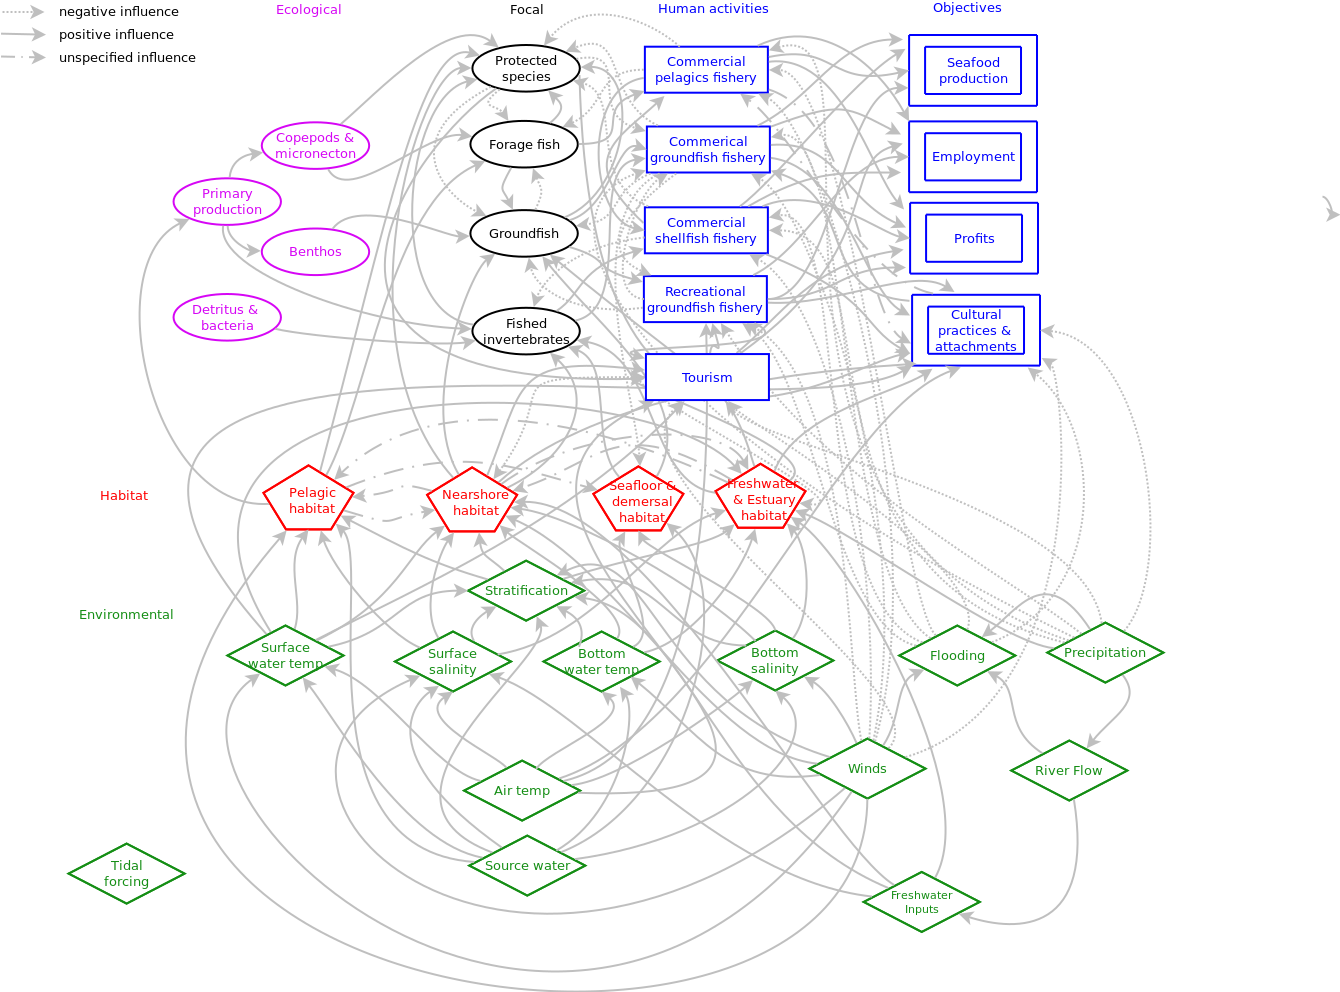
\includegraphics[width=18.61in]{C:/Users/kimberly.bastille/Desktop/tech-doc/images/GoMoverview4} \caption{Gulf of Maine conceptual model}\label{fig:diaGOM}
\end{figure}

\begin{figure}
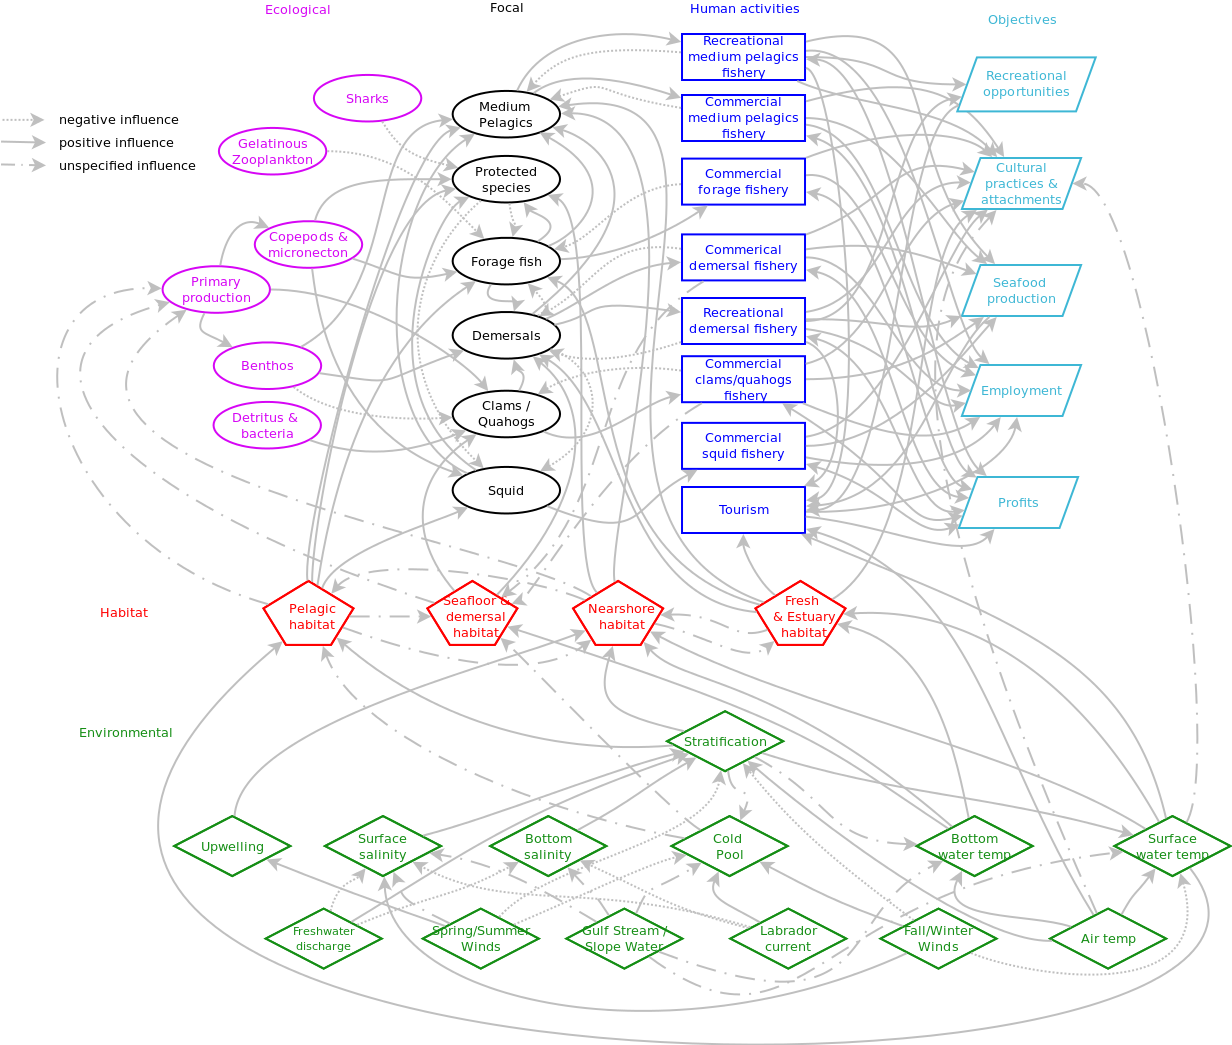
\includegraphics[width=17.11in]{C:/Users/kimberly.bastille/Desktop/tech-doc/images/MAB_3} \caption{Mid-Atlantic Bight conceptual model}\label{fig:diaMAB}
\end{figure}

\subsubsection{Communication tools}\label{communication-tools}

The merged models were redrawn for use in communications with the
public. These versions lead off the State of the Ecosystem reports for
both Fishery Management Councils to provide an overview of linkages
between environmental drivers, ecological, and human systems.

\begin{figure}
\centering
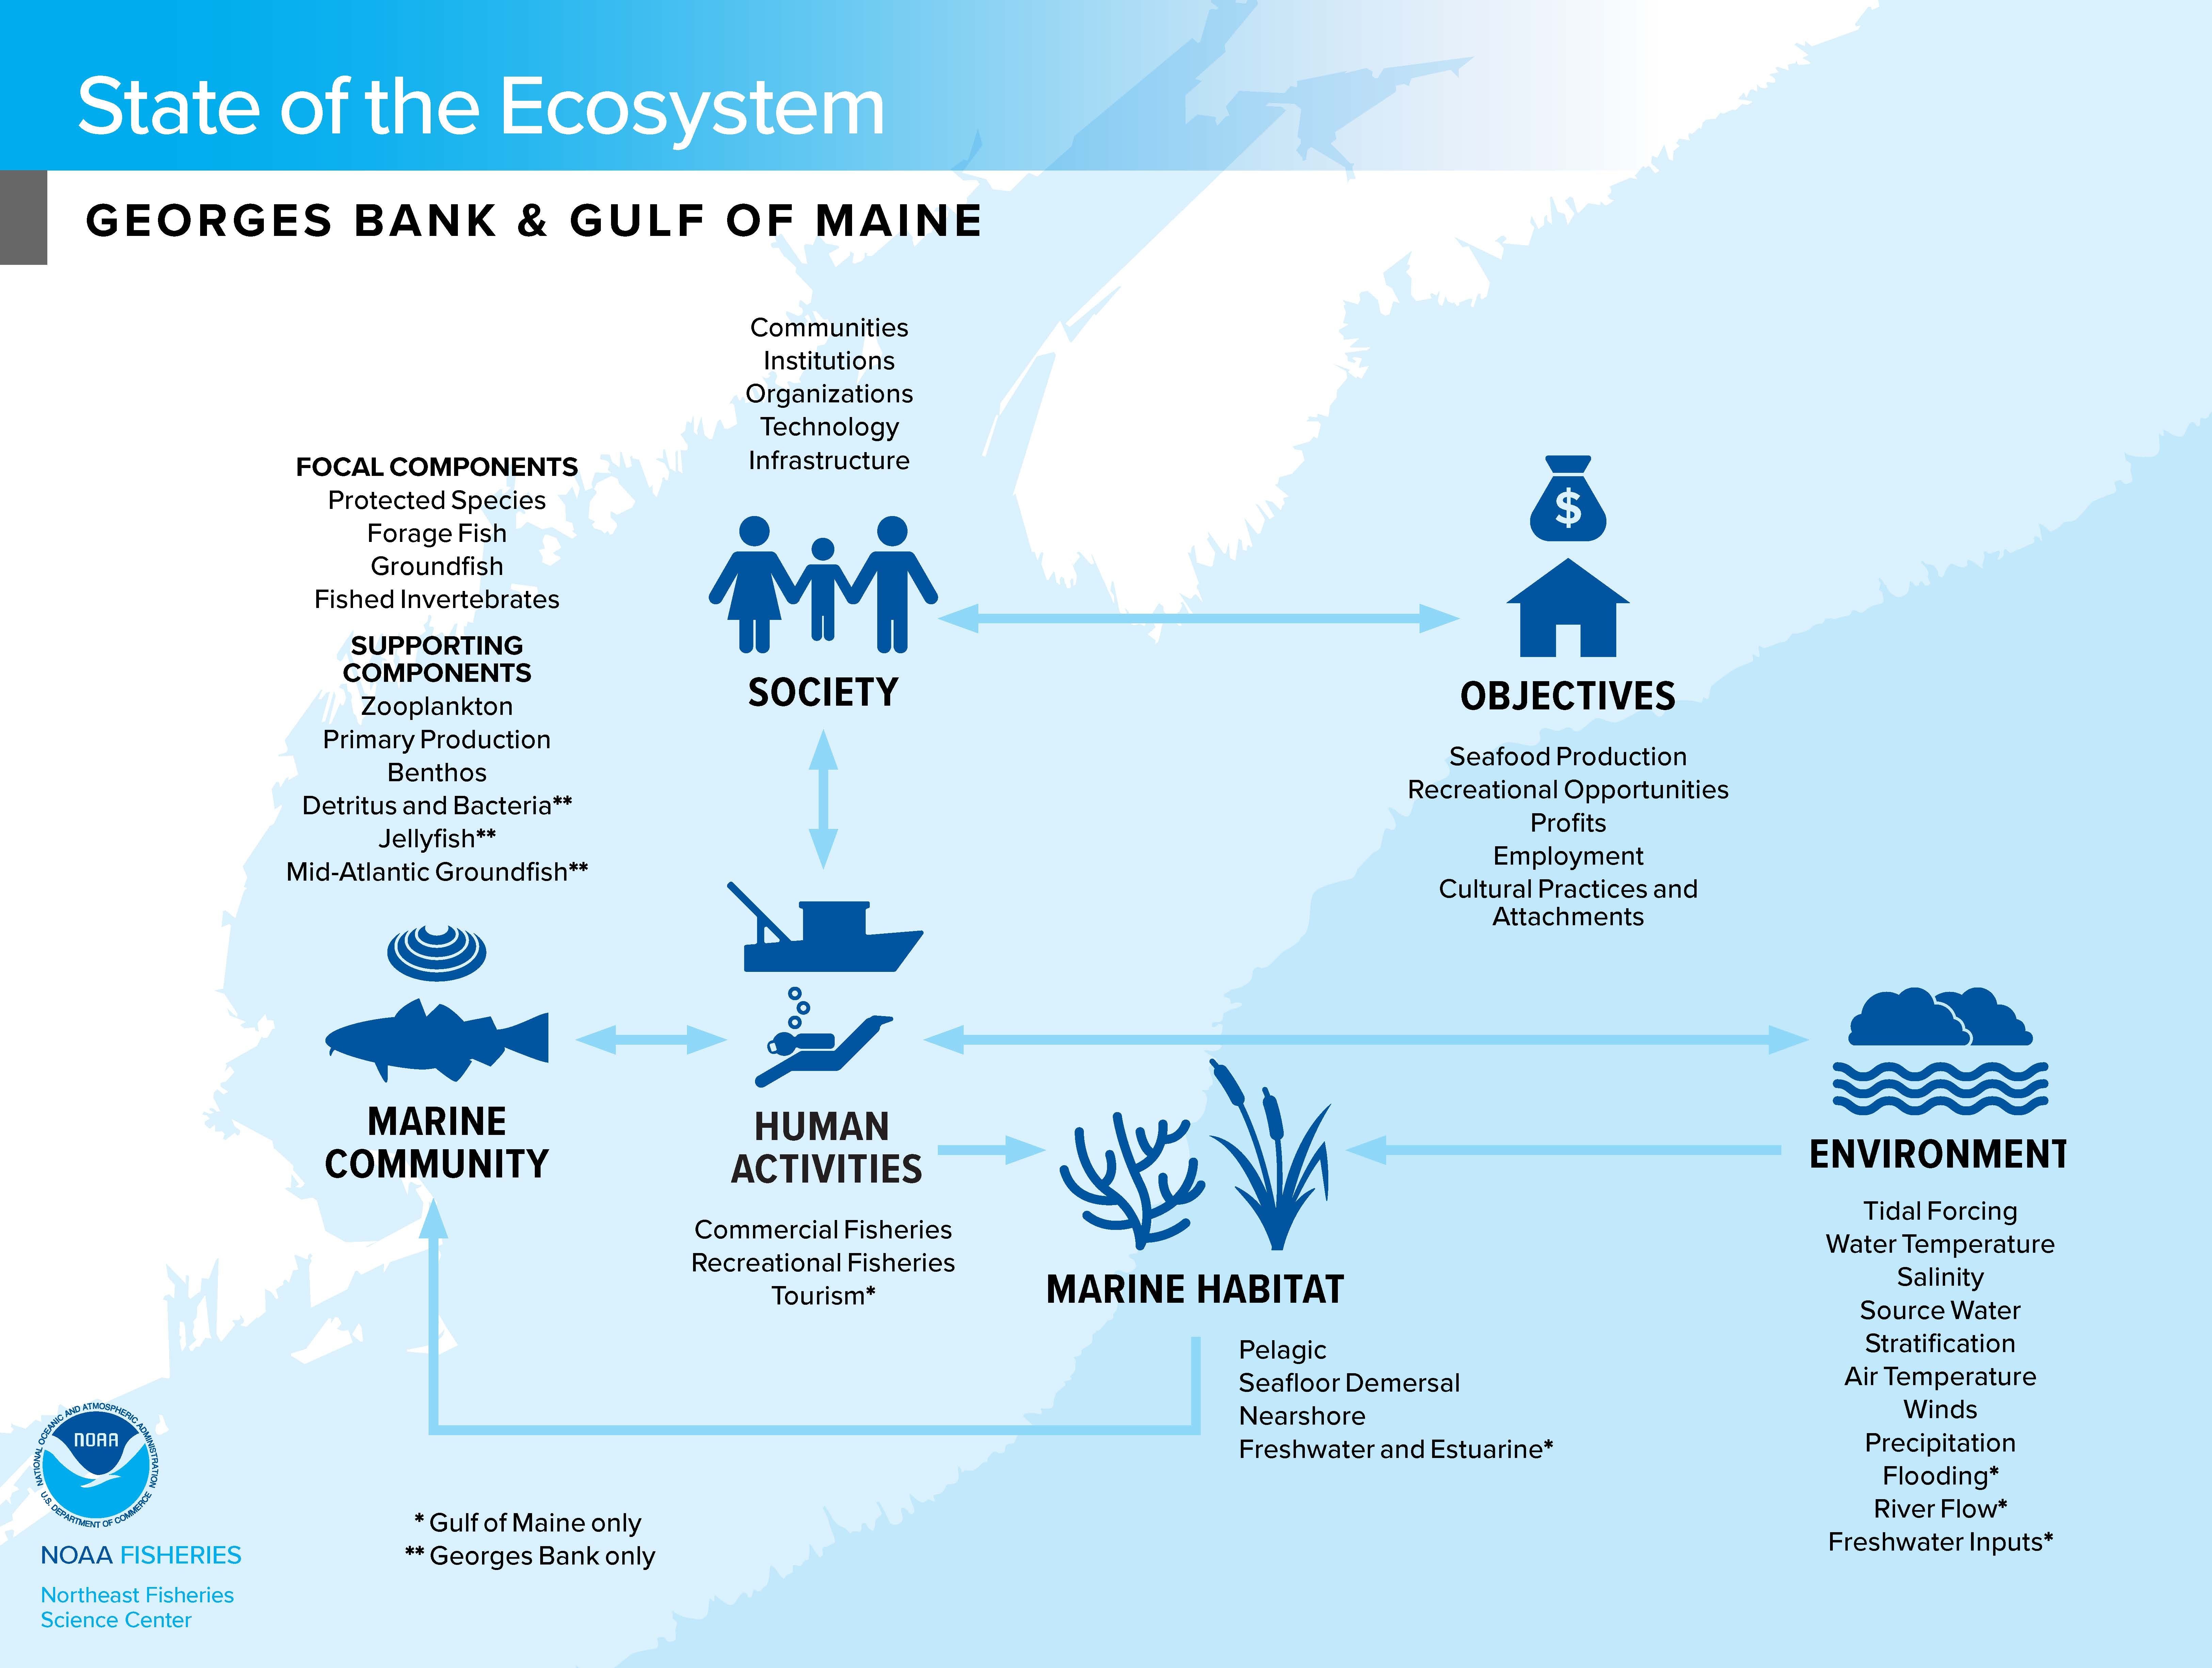
\includegraphics{C:/Users/kimberly.bastille/Desktop/tech-doc/images/GOM_GB_conmod_overview.jpg}
\caption{\label{fig:prettyNE}New England conceptual model for public
communication}
\end{figure}

\begin{figure}
\centering
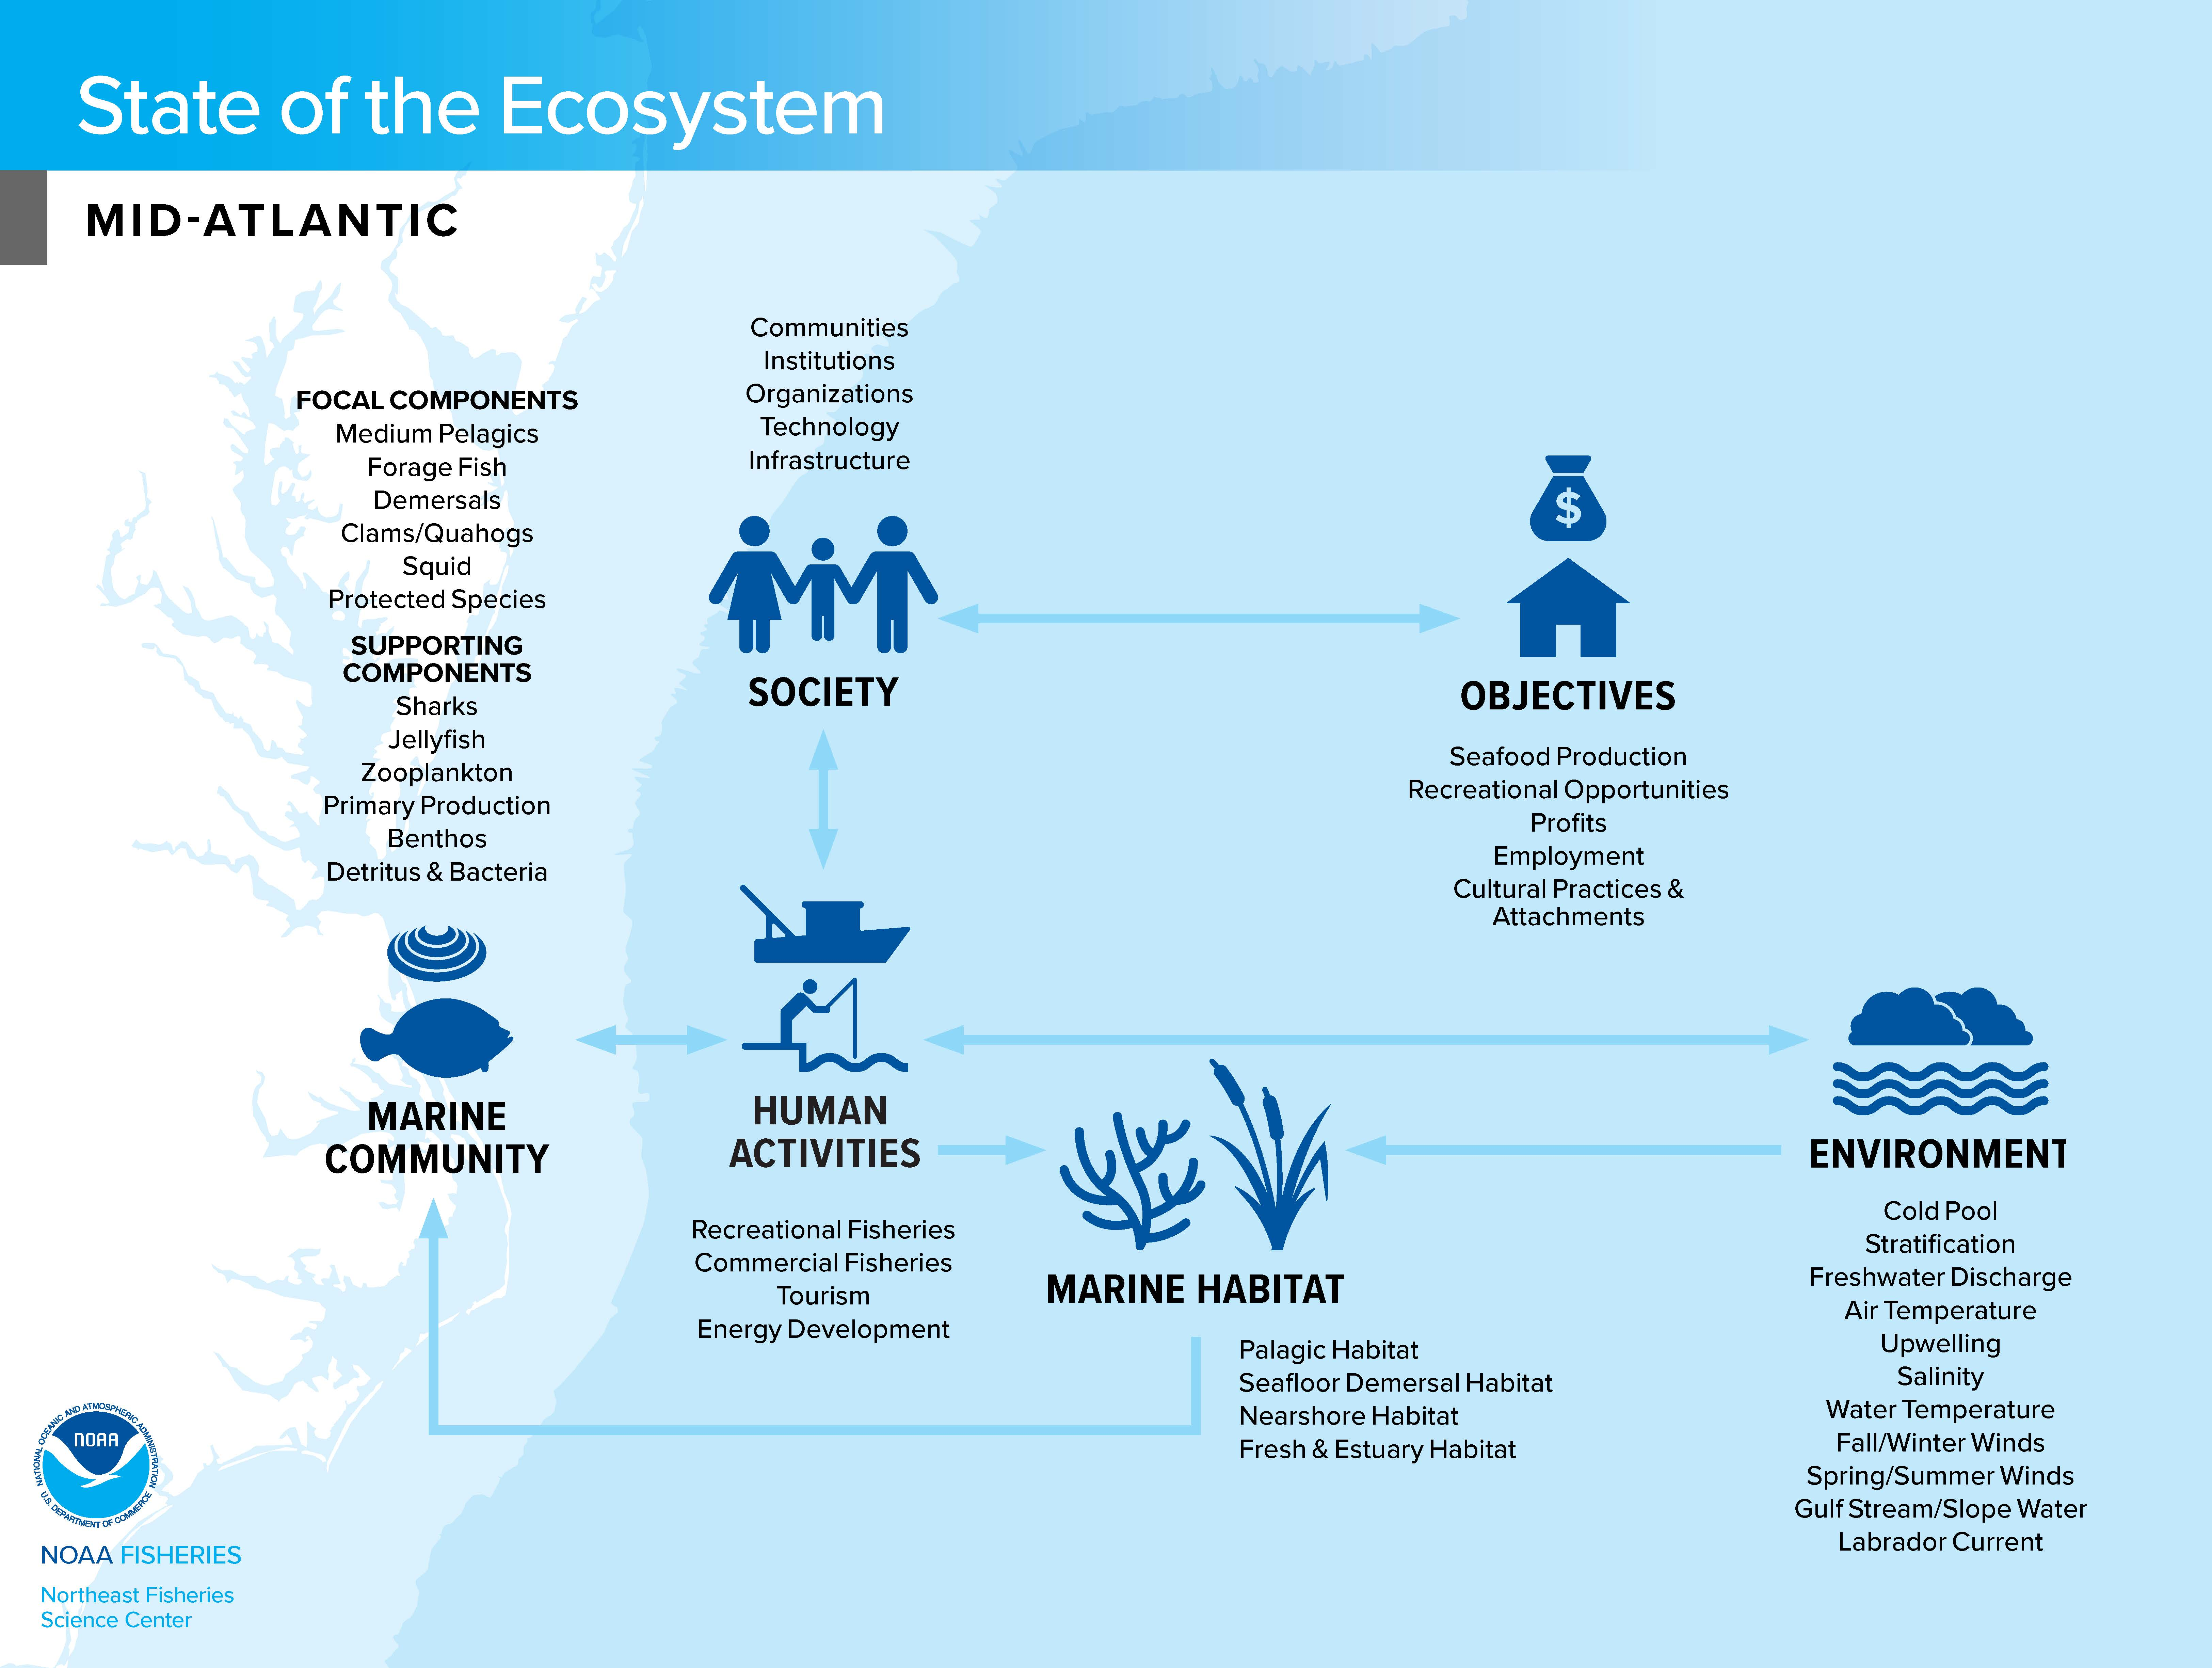
\includegraphics{C:/Users/kimberly.bastille/Desktop/tech-doc/images/MAB_conmod_overview.jpg}
\caption{\label{fig:prettyMA}Mid-Atlantic conceptual model for public
communication}
\end{figure}

\chapter{Fish Condition Indicator}\label{fish-condition-indicator}

\textbf{Description}: Relative condition

\textbf{Found in}: State of the Ecosystem - Gulf of Maine \& Georges
Bank (2018,2019), State of the Ecosystem - Mid-Atlantic (2018,2019)

\textbf{Indicator category}: Database pull with analysis

\textbf{Contributor(s)}: Laurel Smith

\textbf{Data steward}: Laurel Smith,
\href{mailto:laurel.smith@noaa.gov}{\nolinkurl{laurel.smith@noaa.gov}}

\textbf{Point of contact}: Laurel Smith,
\href{mailto:laurel.smith@noaa.gov}{\nolinkurl{laurel.smith@noaa.gov}}

\textbf{Public availability statement}: NEFSC survey data used in these
analyses are available upon request (see
\href{https://inport.nmfs.noaa.gov/inport/item/22560}{BTS metadata} for
access procedures). Derived condition data are available
\href{https://comet.nefsc.noaa.gov/erddap/tabledap/gf_condition_soe_v1.html}{here}.

\section{Methods}\label{methods-10}

Relative condition (Kn) was introduced by Cren
(\protect\hyperlink{ref-Cren1951a}{1951}) as a way to remove the
influence of length on condition, and Blackwell, Brown, and Willis
(\protect\hyperlink{ref-Blackwell2000}{2000}) noted that Kn may be
useful in detecting prolonged physical stress on a fish populations.
Relative condition is calculated as \[Kn = W/W',\] where W is the weight
of an individual fish and W' is the predicted length-specific mean
weight for the fish population in a given region. ``Here, relative
condition was calculated for finfish stocks commonly caught on the
Northeast Fisheries Science Center's (NEFSC) autumn and spring bottom
trawl surveys, from 1992-present.

Where data allowed, predicted length-weight parameters were calculated
for W' by species, sex and season over the time period 1992-2012. When
sample sizes of individual fish weights and lengths were too low,
parameters were calculated for aggregated spring and fall survey data
over the same time period. Fall survey relative condition was calculated
by sex for those species that exhibited differences in growth between
sexes and aggregated across sex for those that did not.

\subsection{Data sources}\label{data-sources-10}

Individual fish lengths (to the nearest 0.5 cm) and weights (grams) were
collected on the NEFSC bottom trawl surveys from 1992-present aboard RVs
Albatross IV, Delaware II and the Henry B. Bigelow (see
\protect\hyperlink{survdat}{Survdat}). A small number of outlier values
were removed when calculating the length-weight parameters.

\subsection{Data extraction}\label{data-extraction-9}

Data were extracted from NEFSC's survey database (SVDBS) using SQL.

SQL query:

\begin{Shaded}
\begin{Highlighting}[]
\KeywordTok{SELECT}\NormalTok{ cruise6,stratum,tow,station,}
  \DataTypeTok{year}\NormalTok{,}\DataTypeTok{month}\NormalTok{,}\DataTypeTok{day}\NormalTok{,}\DataTypeTok{time}\NormalTok{,beglat,beglon,setdepth,}
\NormalTok{  surftemp,bottemp,}
\NormalTok{  svspp,sex,}\FunctionTok{length}\NormalTok{,age,maturity,indid,indwt,stom_volume,stom_wgt, expcatchwt, expcatchnum}
\KeywordTok{from}\NormalTok{ connection }\KeywordTok{to}\NormalTok{ oracle}
\NormalTok{(}\KeywordTok{select}\NormalTok{ b.cruise6,b.stratum,b.tow,b.station,}
\NormalTok{  s.est_year }\DataTypeTok{year}\NormalTok{,est_month }\DataTypeTok{month}\NormalTok{,est_day }\DataTypeTok{day}\NormalTok{,}
  \FunctionTok{substr}\NormalTok{(est_time,}\DecValTok{1}\NormalTok{,}\DecValTok{2}\NormalTok{)||substr(est_time,}\DecValTok{4}\NormalTok{,}\DecValTok{2}\NormalTok{) }\DataTypeTok{time}\NormalTok{,}
  \FunctionTok{round}\NormalTok{(}\FunctionTok{substr}\NormalTok{(beglat,}\DecValTok{1}\NormalTok{,}\DecValTok{2}\NormalTok{) + (}\FunctionTok{substr}\NormalTok{(beglat,}\DecValTok{3}\NormalTok{,}\DecValTok{7}\NormalTok{)/}\DecValTok{60}\NormalTok{),}\DecValTok{6}\NormalTok{) beglat,}
  \FunctionTok{round}\NormalTok{(((}\FunctionTok{substr}\NormalTok{(beglon,}\DecValTok{1}\NormalTok{,}\DecValTok{2}\NormalTok{) + (}\FunctionTok{substr}\NormalTok{(beglon,}\DecValTok{3}\NormalTok{,}\DecValTok{7}\NormalTok{)/}\DecValTok{60}\NormalTok{)) * -}\DecValTok{1}\NormalTok{), }\DecValTok{6}\NormalTok{) beglon,}
\NormalTok{  setdepth,surftemp, bottemp,}
\NormalTok{  b.svspp,sex,}\FunctionTok{length}\NormalTok{,age,maturity,indid,indwt,stom_volume,stom_wgt, expcatchwt, expcatchnum}
\KeywordTok{from}\NormalTok{ union_fscs_svbio b, union_fscs_svcat p, union_fscs_svsta s, svdbs_cruises c}
\KeywordTok{where} 
\NormalTok{  season = }\CharTok{&sson} \KeywordTok{and}
\NormalTok{    b.svspp }\KeywordTok{in}\NormalTok{ (}\StringTok{'013'}\NormalTok{,}\StringTok{'015'}\NormalTok{,}\StringTok{'023'}\NormalTok{,}\StringTok{'026'}\NormalTok{,}\StringTok{'028'}\NormalTok{,}\StringTok{'032'}\NormalTok{,}\StringTok{'072'}\NormalTok{,}\StringTok{'073'}\NormalTok{,}\StringTok{'074'}\NormalTok{,}\StringTok{'075'}\NormalTok{,}\StringTok{'076'}\NormalTok{,}\StringTok{'077'}\NormalTok{,}\StringTok{'078'}\NormalTok{,}\StringTok{'102'}\NormalTok{,}\StringTok{'103'}\NormalTok{,}\StringTok{'104'}\NormalTok{,}\StringTok{'105'}\NormalTok{,}\StringTok{'106'}\NormalTok{,}\StringTok{'107'}\NormalTok{,}\StringTok{'108'}\NormalTok{,}\StringTok{'121'}\NormalTok{,}\StringTok{'131'}\NormalTok{,}\StringTok{'135'}\NormalTok{,}\StringTok{'141'}\NormalTok{,}\StringTok{'143'}\NormalTok{,}\StringTok{'145'}\NormalTok{,}\StringTok{'155'}\NormalTok{,}\StringTok{'164'}\NormalTok{,}\StringTok{'193'}\NormalTok{,}\StringTok{'197'}\NormalTok{) }\KeywordTok{and}
\NormalTok{  (b.cruise6=s.cruise6) }\KeywordTok{and}
\NormalTok{  (c.cruise6=b.cruise6) }\KeywordTok{and}
\NormalTok{  (p.cruise6=c.cruise6) }\KeywordTok{and}
\NormalTok{  (p.stratum=b.stratum) }\KeywordTok{and}
\NormalTok{  (b.stratum=s.stratum) }\KeywordTok{and}
\NormalTok{  (p.station=b.station) }\KeywordTok{and}
\NormalTok{  (b.station=s.station) }\KeywordTok{and}
\NormalTok{  (p.svspp=b.svspp) }\KeywordTok{and}
\NormalTok{  (p.tow=b.tow) }\KeywordTok{and}
\NormalTok{  (b.tow=s.tow) );}

\NormalTok{  %put }\CharTok{&sqlxmsg}\NormalTok{;}
\NormalTok{  %put }\CharTok{&sqlxrc}\NormalTok{;}

\KeywordTok{create} \KeywordTok{view}\NormalTok{ spp }\KeywordTok{as}

\KeywordTok{select}\NormalTok{ comname, svspp}
\KeywordTok{from}\NormalTok{ connection }\KeywordTok{to}\NormalTok{ oracle}
\NormalTok{(}\KeywordTok{select}\NormalTok{ comname, svspp}
\KeywordTok{from}\NormalTok{ svspecies_list);}

\NormalTok{  %put }\CharTok{&sqlxmsg}\NormalTok{;}
\NormalTok{  %put }\CharTok{&sqlxrc}\NormalTok{;}

\KeywordTok{execute}\NormalTok{ (}\KeywordTok{commit}\NormalTok{) }\KeywordTok{by}\NormalTok{ oracle;}
\end{Highlighting}
\end{Shaded}

\subsection{Data analysis}\label{data-analysis-9}

The following growth curve was fit through individual fish lengths and
weights from the NEFSC bottom trawl survey data from 1992-2012 to
produce reference length-weight parameters:

\[\textrm{Weight} = e^{Fall_{coef}} * \textrm{Length}^{Fall_{exp}},\]

where length is in cm and weight is in kg. Fall survey data were used
where sample sizes allowed for growth curve estimation, otherwise data
from spring and fall seasons were combined.

Individual fish lengths from NEFSC fall bottom trawl survey from
1992-2017 were then used to calculate predicted weights using the
reference length-weight parameters. Relative condition (Kn) was
calculated annually by species and sex (for sexually dimorphic species)
by dividing individual fish weights by the predicted weight.

The following R code was used in the analysis:

\begin{Shaded}
\begin{Highlighting}[]
\CommentTok{# Length-weight parameter calculation:}
\ControlFlowTok{function}\NormalTok{ (data, }\DataTypeTok{min.n =} \DecValTok{25}\NormalTok{, }\DataTypeTok{min.range =} \DecValTok{5}\NormalTok{, }\DataTypeTok{data.avail =} \OtherTok{NA}\NormalTok{, }\DataTypeTok{data.avail.bigelow =} \OtherTok{NA}\NormalTok{) }
\NormalTok{\{}
    \ControlFlowTok{if}\NormalTok{(}\KeywordTok{is.null}\NormalTok{(}\KeywordTok{dim}\NormalTok{(data.avail))) data.avail <-}\StringTok{ }\KeywordTok{lw.data.availability}\NormalTok{(data, min.n, min.range)}
\NormalTok{    data.avail <-}\StringTok{ }\NormalTok{data.avail[}\KeywordTok{apply}\NormalTok{(data.avail[,}\DecValTok{2}\OperatorTok{:}\DecValTok{5}\NormalTok{], }\DecValTok{1}\NormalTok{, any),]}
    \ControlFlowTok{if}\NormalTok{(}\KeywordTok{is.null}\NormalTok{(}\KeywordTok{dim}\NormalTok{(data.avail.bigelow)))data.avail.bigelow <-}\StringTok{ }\KeywordTok{lw.data.availability}\NormalTok{(data[data}\OperatorTok{$}\NormalTok{data.source }\OperatorTok{==}\StringTok{ "Bigelow"}\NormalTok{,], min.n, min.range)}
\NormalTok{    data.avail.bigelow <-}\StringTok{ }\NormalTok{data.avail.bigelow[}\KeywordTok{apply}\NormalTok{(data.avail.bigelow[,}\DecValTok{2}\OperatorTok{:}\DecValTok{5}\NormalTok{], }\DecValTok{1}\NormalTok{, any),]}
\NormalTok{    data.spp <-}\StringTok{ }\KeywordTok{as.numeric}\NormalTok{(}\KeywordTok{rownames}\NormalTok{(data.avail[data.avail}\OperatorTok{$}\NormalTok{sex.season }\OperatorTok{==}\StringTok{ }\OtherTok{TRUE}\NormalTok{,]))}
\NormalTok{    lw.output <-}\StringTok{ }\KeywordTok{data.frame}\NormalTok{(}\KeywordTok{matrix}\NormalTok{(}\DataTypeTok{ncol =} \DecValTok{12}\NormalTok{))}
    \KeywordTok{names}\NormalTok{(lw.output) <-}\StringTok{ }\KeywordTok{c}\NormalTok{(}\StringTok{"species.name"}\NormalTok{, }\StringTok{"species.code"}\NormalTok{, }\StringTok{"source"}\NormalTok{, }\StringTok{"sex"}\NormalTok{, }\StringTok{"season"}\NormalTok{, }\StringTok{"slope"}\NormalTok{, }\StringTok{"slope.p"}\NormalTok{, }\StringTok{"intercept"}\NormalTok{, }\StringTok{"intercept.p"}\NormalTok{, }\StringTok{"min.length"}\NormalTok{, }\StringTok{"max.length"}\NormalTok{, }\StringTok{"check.diff"}\NormalTok{)}
    \ControlFlowTok{for}\NormalTok{(sp }\ControlFlowTok{in}\NormalTok{ data.spp)\{}
\NormalTok{        sp.data <-}\StringTok{ }\NormalTok{lw.data[lw.data}\OperatorTok{$}\NormalTok{species }\OperatorTok{==}\StringTok{ }\NormalTok{sp,]}
\NormalTok{        sp.name <-}\StringTok{ }\KeywordTok{unique}\NormalTok{(}\KeywordTok{as.character}\NormalTok{(species.names}\OperatorTok{$}\NormalTok{scientific_name[species.names}\OperatorTok{$}\NormalTok{svspp }\OperatorTok{==}\StringTok{ }\NormalTok{sp]))}
        \KeywordTok{print}\NormalTok{(sp.name)}
\CommentTok{#All model}
        \KeywordTok{print}\NormalTok{(}\StringTok{"Species Level"}\NormalTok{)}
\NormalTok{        this.data <-}\StringTok{ }\KeywordTok{bigelow.test}\NormalTok{(sp.data, data.avail[}\KeywordTok{as.character}\NormalTok{(sp),], data.avail.bigelow[}\KeywordTok{as.character}\NormalTok{(sp),], }\StringTok{"weight.log~length.log"}\NormalTok{, }\StringTok{"species"}\NormalTok{)}
\NormalTok{        ds <-}\StringTok{ }\NormalTok{this.data[[}\DecValTok{2}\NormalTok{]]}
\NormalTok{        this.data <-}\StringTok{ }\NormalTok{this.data[[}\DecValTok{1}\NormalTok{]]}
        \ControlFlowTok{if}\NormalTok{(}\OperatorTok{!}\KeywordTok{is.null}\NormalTok{(}\KeywordTok{dim}\NormalTok{(this.data)))\{}
\NormalTok{            this.model <-}\StringTok{ }\KeywordTok{lm}\NormalTok{(weight.log}\OperatorTok{~}\NormalTok{length.log, }\DataTypeTok{data =}\NormalTok{ this.data)}
\NormalTok{            model.coefs <-}\StringTok{ }\KeywordTok{coef}\NormalTok{(this.model)}
\NormalTok{            model.summary <-}\StringTok{ }\KeywordTok{coef}\NormalTok{(}\KeywordTok{summary}\NormalTok{(this.model))}
\NormalTok{            length.range <-}\StringTok{ }\KeywordTok{range}\NormalTok{(sp.data}\OperatorTok{$}\NormalTok{length)}
\NormalTok{            length.log <-}\StringTok{ }\KeywordTok{log}\NormalTok{(}\KeywordTok{seq}\NormalTok{(length.range[}\DecValTok{1}\NormalTok{], length.range[}\DecValTok{2}\NormalTok{], }\DataTypeTok{by=}\NormalTok{.}\DecValTok{5}\NormalTok{))}
\NormalTok{            species <-}\StringTok{ }\KeywordTok{rep}\NormalTok{(sp, }\KeywordTok{length}\NormalTok{(length.log))}
\NormalTok{            predict.length <-}\StringTok{ }\KeywordTok{data.frame}\NormalTok{(species, length.log)}
\NormalTok{            check.diffs <-}\StringTok{ }\KeywordTok{plot.lw}\NormalTok{(this.data, this.model, }\StringTok{"species"}\NormalTok{, sp.name, predict.length)}
\NormalTok{            lw.output <-}\StringTok{ }\KeywordTok{rbind}\NormalTok{(lw.output, }\KeywordTok{c}\NormalTok{(sp.name, sp, ds, }\OtherTok{NA}\NormalTok{, }\OtherTok{NA}\NormalTok{, model.coefs[}\StringTok{"length.log"}\NormalTok{], model.summary[}\StringTok{"length.log"}\NormalTok{, }\StringTok{"Pr(>|t|)"}\NormalTok{], model.coefs[}\StringTok{"(Intercept)"}\NormalTok{], model.summary[}\StringTok{"(Intercept)"}\NormalTok{, }\StringTok{"Pr(>|t|)"}\NormalTok{], length.range[}\DecValTok{1}\NormalTok{], length.range[}\DecValTok{2}\NormalTok{], check.diffs))}
\NormalTok{        \}}
\CommentTok{#Sex model}
        \KeywordTok{print}\NormalTok{(}\StringTok{"Sex Level"}\NormalTok{)}
\NormalTok{        this.data <-}\StringTok{ }\NormalTok{sp.data[sp.data}\OperatorTok{$}\NormalTok{sex }\OperatorTok{>}\StringTok{ }\DecValTok{0}\NormalTok{,]}
\NormalTok{        model.definition <-}\StringTok{ "weight.log~length.log * factor(sex)"}
\NormalTok{        this.data <-}\StringTok{ }\KeywordTok{bigelow.test}\NormalTok{(this.data, data.avail[}\KeywordTok{as.character}\NormalTok{(sp),], data.avail.bigelow[}\KeywordTok{as.character}\NormalTok{(sp),], model.definition, }\StringTok{"sex"}\NormalTok{)}
\NormalTok{        ds <-}\StringTok{ }\NormalTok{this.data[[}\DecValTok{2}\NormalTok{]]}
\NormalTok{        this.data <-}\StringTok{ }\NormalTok{this.data[[}\DecValTok{1}\NormalTok{]]}
        \ControlFlowTok{if}\NormalTok{(}\OperatorTok{!}\KeywordTok{is.null}\NormalTok{(}\KeywordTok{dim}\NormalTok{(this.data)))\{}
\NormalTok{            this.model <-}\StringTok{ }\KeywordTok{lm}\NormalTok{(weight.log}\OperatorTok{~}\NormalTok{length.log }\OperatorTok{*}\StringTok{ }\KeywordTok{factor}\NormalTok{(sex), }\DataTypeTok{data =}\NormalTok{ this.data)}
\NormalTok{            male.range <-}\StringTok{ }\KeywordTok{range}\NormalTok{(this.data}\OperatorTok{$}\NormalTok{length[this.data}\OperatorTok{$}\NormalTok{sex }\OperatorTok{==}\StringTok{ }\DecValTok{1}\NormalTok{])}
\NormalTok{            female.range <-}\StringTok{ }\KeywordTok{range}\NormalTok{(this.data}\OperatorTok{$}\NormalTok{length[this.data}\OperatorTok{$}\NormalTok{sex }\OperatorTok{==}\StringTok{ }\DecValTok{2}\NormalTok{])         }
\NormalTok{            model.summary <-}\StringTok{ }\KeywordTok{coef}\NormalTok{(}\KeywordTok{summary}\NormalTok{(this.model))}
            \ControlFlowTok{if}\NormalTok{(}\KeywordTok{any}\NormalTok{(model.summary[}\KeywordTok{grep}\NormalTok{(}\StringTok{"sex"}\NormalTok{, }\KeywordTok{rownames}\NormalTok{(model.summary)), }\StringTok{"Pr(>|t|)"}\NormalTok{] }\OperatorTok{<=}\StringTok{ }\NormalTok{.}\DecValTok{05}\NormalTok{))\{}
\NormalTok{                model.coefs <-}\StringTok{ }\KeywordTok{coef}\NormalTok{(this.model)}
\NormalTok{                length.log <-}\StringTok{ }\KeywordTok{rep}\NormalTok{(}\KeywordTok{log}\NormalTok{(}\KeywordTok{seq}\NormalTok{(length.range[}\DecValTok{1}\NormalTok{], length.range[}\DecValTok{2}\NormalTok{], }\DataTypeTok{by=}\NormalTok{.}\DecValTok{5}\NormalTok{)),}\DecValTok{2}\NormalTok{)}
\NormalTok{                sex <-}\StringTok{ }\KeywordTok{c}\NormalTok{(}\KeywordTok{rep}\NormalTok{(}\DecValTok{1}\NormalTok{, }\KeywordTok{length}\NormalTok{(length.log)}\OperatorTok{/}\DecValTok{2}\NormalTok{), }\KeywordTok{rep}\NormalTok{(}\DecValTok{2}\NormalTok{, }\KeywordTok{length}\NormalTok{(length.log)}\OperatorTok{/}\DecValTok{2}\NormalTok{))}
\NormalTok{                predict.length <-}\StringTok{ }\KeywordTok{data.frame}\NormalTok{(length.log, sex)}
\NormalTok{                check.diffs <-}\StringTok{ }\KeywordTok{plot.lw}\NormalTok{(this.data, this.model, }\StringTok{"sex"}\NormalTok{, sp.name, predict.length)}
\NormalTok{                lw.output <-}\StringTok{ }\KeywordTok{rbind}\NormalTok{(lw.output, }\KeywordTok{c}\NormalTok{(sp.name, sp, ds, }\DecValTok{1}\NormalTok{, }\OtherTok{NA}\NormalTok{, model.coefs[}\StringTok{"length.log"}\NormalTok{], model.summary[}\StringTok{"length.log"}\NormalTok{, }\StringTok{"Pr(>|t|)"}\NormalTok{], model.coefs[}\StringTok{"(Intercept)"}\NormalTok{], model.summary[}\StringTok{"(Intercept)"}\NormalTok{, }\StringTok{"Pr(>|t|)"}\NormalTok{], male.range[}\DecValTok{1}\NormalTok{], male.range[}\DecValTok{2}\NormalTok{], check.diffs[}\DecValTok{1}\NormalTok{]))}
\NormalTok{                lw.output <-}\StringTok{ }\KeywordTok{rbind}\NormalTok{(lw.output, }\KeywordTok{c}\NormalTok{(sp.name, sp, ds, }\DecValTok{2}\NormalTok{, }\OtherTok{NA}\NormalTok{, model.coefs[}\StringTok{"length.log"}\NormalTok{] }\OperatorTok{+}\StringTok{ }\NormalTok{model.coefs[}\StringTok{"length.log:factor(sex)2"}\NormalTok{], model.summary[}\StringTok{"length.log:factor(sex)2"}\NormalTok{, }\StringTok{"Pr(>|t|)"}\NormalTok{], model.coefs[}\StringTok{"(Intercept)"}\NormalTok{] }\OperatorTok{+}\StringTok{ }\NormalTok{model.coefs[}\StringTok{"factor(sex)2"}\NormalTok{], model.summary[}\StringTok{"factor(sex)2"}\NormalTok{, }\StringTok{"Pr(>|t|)"}\NormalTok{], female.range[}\DecValTok{1}\NormalTok{], female.range[}\DecValTok{2}\NormalTok{], check.diffs[}\DecValTok{2}\NormalTok{]))}
\NormalTok{            \}}
            \ControlFlowTok{else}\NormalTok{\{}
                \KeywordTok{print}\NormalTok{(}\KeywordTok{paste}\NormalTok{(}\StringTok{"Model parameters not significantly different for"}\NormalTok{, model.definition))}
\NormalTok{            \}}
\NormalTok{        \}}
\CommentTok{#Season model}
\NormalTok{        model.definition <-}\StringTok{ "weight.log~length.log * factor(season)"}
\NormalTok{        this.data <-}\StringTok{ }\KeywordTok{bigelow.test}\NormalTok{(sp.data, data.avail[}\KeywordTok{as.character}\NormalTok{(sp),], data.avail.bigelow[}\KeywordTok{as.character}\NormalTok{(sp),], model.definition, }\StringTok{"season"}\NormalTok{)}
\NormalTok{        ds <-}\StringTok{ }\NormalTok{this.data[[}\DecValTok{2}\NormalTok{]]}
\NormalTok{        this.data <-}\StringTok{ }\NormalTok{this.data[[}\DecValTok{1}\NormalTok{]]}
        \ControlFlowTok{if}\NormalTok{(}\OperatorTok{!}\KeywordTok{is.null}\NormalTok{(}\KeywordTok{dim}\NormalTok{(this.data)))\{}
\NormalTok{            this.model <-}\StringTok{ }\KeywordTok{lm}\NormalTok{(weight.log}\OperatorTok{~}\NormalTok{length.log }\OperatorTok{*}\StringTok{ }\KeywordTok{factor}\NormalTok{(season), }\DataTypeTok{data =}\NormalTok{ this.data)}
\NormalTok{            fall.range <-}\StringTok{ }\KeywordTok{range}\NormalTok{(this.data}\OperatorTok{$}\NormalTok{length[this.data}\OperatorTok{$}\NormalTok{season }\OperatorTok{==}\StringTok{ "FALL"}\NormalTok{])}
\NormalTok{            spring.range <-}\StringTok{ }\KeywordTok{range}\NormalTok{(this.data}\OperatorTok{$}\NormalTok{length[this.data}\OperatorTok{$}\NormalTok{season }\OperatorTok{==}\StringTok{ "SPRING"}\NormalTok{])}
\NormalTok{            model.summary <-}\StringTok{ }\KeywordTok{coef}\NormalTok{(}\KeywordTok{summary}\NormalTok{(this.model))}
            \ControlFlowTok{if}\NormalTok{(}\KeywordTok{any}\NormalTok{(model.summary[}\KeywordTok{grep}\NormalTok{(}\StringTok{"season"}\NormalTok{, }\KeywordTok{rownames}\NormalTok{(model.summary)), }\StringTok{"Pr(>|t|)"}\NormalTok{] }\OperatorTok{<=}\StringTok{ }\NormalTok{.}\DecValTok{05}\NormalTok{))\{}
\NormalTok{                model.coefs <-}\StringTok{ }\KeywordTok{coef}\NormalTok{(this.model)}
\NormalTok{                length.log <-}\StringTok{ }\KeywordTok{rep}\NormalTok{(}\KeywordTok{log}\NormalTok{(}\KeywordTok{seq}\NormalTok{(length.range[}\DecValTok{1}\NormalTok{], length.range[}\DecValTok{2}\NormalTok{], }\DataTypeTok{by=}\NormalTok{.}\DecValTok{5}\NormalTok{)),}\DecValTok{2}\NormalTok{)}
\NormalTok{                season <-}\StringTok{ }\KeywordTok{c}\NormalTok{(}\KeywordTok{rep}\NormalTok{(}\StringTok{"FALL"}\NormalTok{, }\KeywordTok{length}\NormalTok{(length.log)}\OperatorTok{/}\DecValTok{2}\NormalTok{), }\KeywordTok{rep}\NormalTok{(}\StringTok{"SPRING"}\NormalTok{, }\KeywordTok{length}\NormalTok{(length.log)}\OperatorTok{/}\DecValTok{2}\NormalTok{))}
\NormalTok{                predict.length <-}\StringTok{ }\KeywordTok{data.frame}\NormalTok{(length.log, season)}
\NormalTok{                check.diffs <-}\StringTok{ }\KeywordTok{plot.lw}\NormalTok{(this.data, this.model, }\StringTok{"season"}\NormalTok{, sp.name, predict.length)}
\NormalTok{                lw.output <-}\StringTok{ }\KeywordTok{rbind}\NormalTok{(lw.output, }\KeywordTok{c}\NormalTok{(sp.name, sp, ds, }\OtherTok{NA}\NormalTok{, }\StringTok{"FALL"}\NormalTok{, model.coefs[}\StringTok{"length.log"}\NormalTok{], model.summary[}\StringTok{"length.log"}\NormalTok{, }\StringTok{"Pr(>|t|)"}\NormalTok{], model.coefs[}\StringTok{"(Intercept)"}\NormalTok{], model.summary[}\StringTok{"(Intercept)"}\NormalTok{, }\StringTok{"Pr(>|t|)"}\NormalTok{], fall.range[}\DecValTok{1}\NormalTok{], fall.range[}\DecValTok{2}\NormalTok{], check.diffs[}\DecValTok{1}\NormalTok{]))}
\NormalTok{                lw.output <-}\StringTok{ }\KeywordTok{rbind}\NormalTok{(lw.output, }\KeywordTok{c}\NormalTok{(sp.name, sp, ds, }\OtherTok{NA}\NormalTok{, }\StringTok{"SPRING"}\NormalTok{, model.coefs[}\StringTok{"length.log"}\NormalTok{] }\OperatorTok{+}\StringTok{ }\NormalTok{model.coefs[}\StringTok{"length.log:factor(season)SPRING"}\NormalTok{], model.summary[}\StringTok{"length.log:factor(season)SPRING"}\NormalTok{, }\StringTok{"Pr(>|t|)"}\NormalTok{], model.coefs[}\StringTok{"(Intercept)"}\NormalTok{] }\OperatorTok{+}\StringTok{ }\NormalTok{model.coefs[}\StringTok{"factor(season)SPRING"}\NormalTok{], model.summary[}\StringTok{"factor(season)SPRING"}\NormalTok{, }\StringTok{"Pr(>|t|)"}\NormalTok{], spring.range[}\DecValTok{1}\NormalTok{], spring.range[}\DecValTok{2}\NormalTok{], check.diffs[}\DecValTok{1}\NormalTok{]))}
\NormalTok{            \}}
            \ControlFlowTok{else}\NormalTok{\{}
                \KeywordTok{print}\NormalTok{(}\KeywordTok{paste}\NormalTok{(}\StringTok{"Model parameters not significantly different for"}\NormalTok{, model.definition))}
\NormalTok{            \}}
\NormalTok{        \}}
\CommentTok{#Sex-Season model}
\NormalTok{        this.data <-}\StringTok{ }\NormalTok{sp.data[sp.data}\OperatorTok{$}\NormalTok{sex }\OperatorTok{>}\StringTok{ }\DecValTok{0}\NormalTok{,]}
\NormalTok{        model.definition <-}\StringTok{ "weight.log~length.log * factor(sex) * factor(season)"}
\NormalTok{        this.data <-}\StringTok{ }\KeywordTok{bigelow.test}\NormalTok{(this.data, data.avail[}\KeywordTok{as.character}\NormalTok{(sp),], data.avail.bigelow[}\KeywordTok{as.character}\NormalTok{(sp),], model.definition, }\KeywordTok{c}\NormalTok{(}\StringTok{"sex"}\NormalTok{,}\StringTok{"season"}\NormalTok{))}
\NormalTok{        ds <-}\StringTok{ }\NormalTok{this.data[[}\DecValTok{2}\NormalTok{]]}
\NormalTok{        this.data <-}\StringTok{ }\NormalTok{this.data[[}\DecValTok{1}\NormalTok{]]}
        \ControlFlowTok{if}\NormalTok{(}\OperatorTok{!}\KeywordTok{is.null}\NormalTok{(}\KeywordTok{dim}\NormalTok{(this.data)))\{}
\NormalTok{            this.model <-}\StringTok{ }\KeywordTok{lm}\NormalTok{(weight.log}\OperatorTok{~}\NormalTok{length.log }\OperatorTok{*}\StringTok{ }\KeywordTok{factor}\NormalTok{(sex) }\OperatorTok{*}\StringTok{ }\KeywordTok{factor}\NormalTok{(season), }\DataTypeTok{data =}\NormalTok{ this.data)}
\NormalTok{            model.summary <-}\StringTok{ }\KeywordTok{coef}\NormalTok{(}\KeywordTok{summary}\NormalTok{(this.model))}
\NormalTok{            male.fall.range <-}\StringTok{ }\KeywordTok{range}\NormalTok{(this.data}\OperatorTok{$}\NormalTok{length[this.data}\OperatorTok{$}\NormalTok{season }\OperatorTok{==}\StringTok{ "FALL"} \OperatorTok{&}\StringTok{ }\NormalTok{this.data}\OperatorTok{$}\NormalTok{sex }\OperatorTok{==}\StringTok{ }\DecValTok{1}\NormalTok{])}
\NormalTok{            male.spring.range <-}\StringTok{ }\KeywordTok{range}\NormalTok{(this.data}\OperatorTok{$}\NormalTok{length[this.data}\OperatorTok{$}\NormalTok{season }\OperatorTok{==}\StringTok{ "SPRING"} \OperatorTok{&}\StringTok{ }\NormalTok{this.data}\OperatorTok{$}\NormalTok{sex }\OperatorTok{==}\StringTok{ }\DecValTok{1}\NormalTok{])}
\NormalTok{            female.fall.range <-}\StringTok{ }\KeywordTok{range}\NormalTok{(this.data}\OperatorTok{$}\NormalTok{length[this.data}\OperatorTok{$}\NormalTok{season }\OperatorTok{==}\StringTok{ "FALL"} \OperatorTok{&}\StringTok{ }\NormalTok{this.data}\OperatorTok{$}\NormalTok{sex }\OperatorTok{==}\StringTok{ }\DecValTok{2}\NormalTok{])}
\NormalTok{            female.spring.range <-}\StringTok{ }\KeywordTok{range}\NormalTok{(this.data}\OperatorTok{$}\NormalTok{length[this.data}\OperatorTok{$}\NormalTok{season }\OperatorTok{==}\StringTok{ "SPRING"} \OperatorTok{&}\StringTok{ }\NormalTok{this.data}\OperatorTok{$}\NormalTok{sex }\OperatorTok{==}\StringTok{ }\DecValTok{2}\NormalTok{])}
            \ControlFlowTok{if}\NormalTok{(}\KeywordTok{any}\NormalTok{(model.summary[}\KeywordTok{grep}\NormalTok{(}\StringTok{"season"}\NormalTok{, }\KeywordTok{rownames}\NormalTok{(model.summary)), }\StringTok{"Pr(>|t|)"}\NormalTok{] }\OperatorTok{<=}\StringTok{ }\NormalTok{.}\DecValTok{05} \OperatorTok{|}\StringTok{ }\KeywordTok{any}\NormalTok{(model.summary[}\KeywordTok{grep}\NormalTok{(}\StringTok{"season"}\NormalTok{, }\KeywordTok{rownames}\NormalTok{(model.summary)), }\StringTok{"Pr(>|t|)"}\NormalTok{] }\OperatorTok{<=}\StringTok{ }\NormalTok{.}\DecValTok{05}\NormalTok{)))\{}
\NormalTok{                model.coefs <-}\StringTok{ }\KeywordTok{coef}\NormalTok{(this.model)}
\NormalTok{                male.fall.int <-}\StringTok{ }\NormalTok{model.coefs[}\StringTok{"(Intercept)"}\NormalTok{]}
\NormalTok{                male.fall.int.p <-}\StringTok{ }\NormalTok{model.summary[}\StringTok{"(Intercept)"}\NormalTok{, }\StringTok{"Pr(>|t|)"}\NormalTok{]}
\NormalTok{                male.fall.slope <-}\StringTok{ }\NormalTok{model.coefs[}\StringTok{"length.log"}\NormalTok{]}
\NormalTok{                male.fall.slope.p <-}\StringTok{ }\NormalTok{model.summary[}\StringTok{"length.log"}\NormalTok{, }\StringTok{"Pr(>|t|)"}\NormalTok{]}
\NormalTok{                male.spring.int <-}\StringTok{ }\NormalTok{male.fall.int }\OperatorTok{+}\StringTok{ }\NormalTok{model.coefs[}\StringTok{"factor(season)SPRING"}\NormalTok{]}
\NormalTok{                male.spring.int.p <-}\StringTok{ }\NormalTok{model.summary[}\StringTok{"factor(season)SPRING"}\NormalTok{, }\StringTok{"Pr(>|t|)"}\NormalTok{]}
\NormalTok{                male.spring.slope <-}\StringTok{ }\NormalTok{male.fall.slope }\OperatorTok{+}\StringTok{ }\NormalTok{model.coefs[}\StringTok{"length.log:factor(season)SPRING"}\NormalTok{]}
\NormalTok{                male.spring.slope.p <-}\StringTok{ }\NormalTok{model.summary[}\StringTok{"length.log:factor(season)SPRING"}\NormalTok{, }\StringTok{"Pr(>|t|)"}\NormalTok{]}
\NormalTok{                female.fall.int <-}\StringTok{ }\NormalTok{male.fall.int }\OperatorTok{+}\StringTok{ }\NormalTok{model.coefs[}\StringTok{"factor(sex)2"}\NormalTok{]}
\NormalTok{                female.fall.int.p <-}\StringTok{ }\NormalTok{model.summary[}\StringTok{"factor(sex)2"}\NormalTok{, }\StringTok{"Pr(>|t|)"}\NormalTok{]}
\NormalTok{                female.fall.slope <-}\StringTok{ }\NormalTok{male.fall.slope }\OperatorTok{+}\StringTok{ }\NormalTok{model.coefs[}\StringTok{"length.log:factor(sex)2"}\NormalTok{]}
\NormalTok{                female.fall.slope.p <-}\StringTok{ }\NormalTok{model.summary[}\StringTok{"length.log:factor(sex)2"}\NormalTok{, }\StringTok{"Pr(>|t|)"}\NormalTok{]}
\NormalTok{                female.spring.int <-}\StringTok{ }\NormalTok{male.spring.int }\OperatorTok{+}\StringTok{ }\NormalTok{model.coefs[}\StringTok{"factor(sex)2"}\NormalTok{] }\OperatorTok{+}\StringTok{ }\NormalTok{model.coefs[}\StringTok{"factor(sex)2:factor(season)SPRING"}\NormalTok{]}
\NormalTok{                female.spring.int.p <-}\StringTok{ }\NormalTok{model.summary[}\StringTok{"factor(sex)2:factor(season)SPRING"}\NormalTok{,  }\StringTok{"Pr(>|t|)"}\NormalTok{]}
\NormalTok{                female.spring.slope <-}\StringTok{ }\NormalTok{male.spring.slope }\OperatorTok{+}\StringTok{ }\NormalTok{model.coefs[}\StringTok{"length.log:factor(sex)2"}\NormalTok{] }\OperatorTok{+}\StringTok{ }\NormalTok{model.coefs[}\StringTok{"length.log:factor(sex)2:factor(season)SPRING"}\NormalTok{]}
\NormalTok{                female.spring.slope.p <-}\StringTok{ }\NormalTok{model.summary[}\StringTok{"length.log:factor(sex)2:factor(season)SPRING"}\NormalTok{, }\StringTok{"Pr(>|t|)"}\NormalTok{]}
\NormalTok{                length.log <-}\StringTok{ }\KeywordTok{rep}\NormalTok{(}\KeywordTok{log}\NormalTok{(}\KeywordTok{seq}\NormalTok{(length.range[}\DecValTok{1}\NormalTok{], length.range[}\DecValTok{2}\NormalTok{], }\DataTypeTok{by=}\NormalTok{.}\DecValTok{5}\NormalTok{)),}\DecValTok{4}\NormalTok{)}
\NormalTok{                sex <-}\StringTok{ }\KeywordTok{c}\NormalTok{(}\KeywordTok{rep}\NormalTok{(}\StringTok{"1"}\NormalTok{, }\KeywordTok{length}\NormalTok{(length.log)}\OperatorTok{/}\DecValTok{2}\NormalTok{), }\KeywordTok{rep}\NormalTok{(}\StringTok{"2"}\NormalTok{, }\KeywordTok{length}\NormalTok{(length.log)}\OperatorTok{/}\DecValTok{2}\NormalTok{))}
\NormalTok{                season <-}\StringTok{ }\KeywordTok{rep}\NormalTok{(}\KeywordTok{c}\NormalTok{(}\KeywordTok{rep}\NormalTok{(}\StringTok{"FALL"}\NormalTok{, }\KeywordTok{length}\NormalTok{(length.log)}\OperatorTok{/}\DecValTok{4}\NormalTok{), }\KeywordTok{rep}\NormalTok{(}\StringTok{"SPRING"}\NormalTok{, }\KeywordTok{length}\NormalTok{(length.log)}\OperatorTok{/}\DecValTok{4}\NormalTok{)),}\DecValTok{2}\NormalTok{)}
\NormalTok{                predict.length <-}\StringTok{ }\KeywordTok{data.frame}\NormalTok{(length.log, sex, season)}
\NormalTok{                check.diffs <-}\StringTok{ }\KeywordTok{plot.lw}\NormalTok{(this.data, this.model, }\KeywordTok{c}\NormalTok{(}\StringTok{"sex"}\NormalTok{, }\StringTok{"season"}\NormalTok{), sp.name, predict.length)}
\NormalTok{                lw.output <-}\StringTok{ }\KeywordTok{rbind}\NormalTok{(lw.output, }\KeywordTok{c}\NormalTok{(sp.name, sp, ds, }\DecValTok{1}\NormalTok{, }\StringTok{"FALL"}\NormalTok{, male.fall.slope, male.fall.slope.p, male.fall.int, male.fall.int.p, male.fall.range[}\DecValTok{1}\NormalTok{], male.fall.range[}\DecValTok{2}\NormalTok{], check.diffs[}\DecValTok{1}\NormalTok{]))}
\NormalTok{                lw.output <-}\StringTok{ }\KeywordTok{rbind}\NormalTok{(lw.output, }\KeywordTok{c}\NormalTok{(sp.name, sp, ds, }\DecValTok{1}\NormalTok{, }\StringTok{"SPRING"}\NormalTok{, male.spring.slope, male.spring.slope.p, male.spring.int, male.spring.int.p, male.spring.range[}\DecValTok{1}\NormalTok{], male.spring.range[}\DecValTok{2}\NormalTok{],check.diffs[}\DecValTok{2}\NormalTok{]))}
\NormalTok{                lw.output <-}\StringTok{ }\KeywordTok{rbind}\NormalTok{(lw.output, }\KeywordTok{c}\NormalTok{(sp.name, sp, ds, }\DecValTok{2}\NormalTok{, }\StringTok{"FALL"}\NormalTok{, female.fall.slope, female.fall.slope.p, female.fall.int, female.fall.int.p, female.fall.range[}\DecValTok{1}\NormalTok{], female.fall.range[}\DecValTok{2}\NormalTok{],check.diffs[}\DecValTok{3}\NormalTok{]))}
\NormalTok{                lw.output <-}\StringTok{ }\KeywordTok{rbind}\NormalTok{(lw.output, }\KeywordTok{c}\NormalTok{(sp.name, sp, ds, }\DecValTok{2}\NormalTok{, }\StringTok{"SPRING"}\NormalTok{, female.spring.slope, female.spring.slope.p, female.spring.int, female.spring.int.p, female.spring.range[}\DecValTok{1}\NormalTok{], female.spring.range[}\DecValTok{2}\NormalTok{],check.diffs[}\DecValTok{4}\NormalTok{]))}
\NormalTok{            \}}
            \ControlFlowTok{else}\NormalTok{\{}
                \KeywordTok{print}\NormalTok{(}\KeywordTok{paste}\NormalTok{(}\StringTok{"Model parameters not significantly different for"}\NormalTok{, model.definition))}
\NormalTok{            \}}
\NormalTok{        \}}
\NormalTok{    \}}
\NormalTok{lw.output <-}\StringTok{ }\NormalTok{lw.output[}\OperatorTok{!}\KeywordTok{is.na}\NormalTok{(lw.output}\OperatorTok{$}\NormalTok{species.code),]}
\NormalTok{lw.output}
\NormalTok{\}}
\CommentTok{#Relative Condition:}
\NormalTok{proc import datafile =}\StringTok{ "lw_parameters.csv"}
\NormalTok{ out =}\StringTok{ }\NormalTok{LWparams}
\NormalTok{ dbms =}\StringTok{ }\NormalTok{csv}
\NormalTok{ replace;}
\NormalTok{ getnames =}\StringTok{ }\NormalTok{yes;}
\NormalTok{run;}

\NormalTok{data LWparams; set LWparams;}
 \ControlFlowTok{if}\NormalTok{ LW_SVSPP =}\StringTok{ }\DecValTok{13}\NormalTok{ then svspp =}\StringTok{ '013'}\NormalTok{;}
 \ControlFlowTok{if}\NormalTok{ LW_SVSPP =}\StringTok{ }\DecValTok{15}\NormalTok{ then svspp =}\StringTok{ '015'}\NormalTok{;}
 \ControlFlowTok{if}\NormalTok{ LW_SVSPP =}\StringTok{ }\DecValTok{23}\NormalTok{ then svspp =}\StringTok{ '023'}\NormalTok{;}
 \ControlFlowTok{if}\NormalTok{ LW_SVSPP =}\StringTok{ }\DecValTok{26}\NormalTok{ then svspp =}\StringTok{ '026'}\NormalTok{;}
 \ControlFlowTok{if}\NormalTok{ LW_SVSPP =}\StringTok{ }\DecValTok{28}\NormalTok{ then svspp =}\StringTok{ '028'}\NormalTok{;}
 \ControlFlowTok{if}\NormalTok{ LW_SVSPP =}\StringTok{ }\DecValTok{32}\NormalTok{ then svspp =}\StringTok{ '032'}\NormalTok{;}
 \ControlFlowTok{if}\NormalTok{ LW_SVSPP =}\StringTok{ }\DecValTok{72}\NormalTok{ then svspp =}\StringTok{ '072'}\NormalTok{;}
 \ControlFlowTok{if}\NormalTok{ LW_SVSPP =}\StringTok{ }\DecValTok{73}\NormalTok{ then svspp =}\StringTok{ '073'}\NormalTok{;}
 \ControlFlowTok{if}\NormalTok{ LW_SVSPP =}\StringTok{ }\DecValTok{74}\NormalTok{ then svspp =}\StringTok{ '074'}\NormalTok{;}
 \ControlFlowTok{if}\NormalTok{ LW_SVSPP =}\StringTok{ }\DecValTok{75}\NormalTok{ then svspp =}\StringTok{ '075'}\NormalTok{;}
 \ControlFlowTok{if}\NormalTok{ LW_SVSPP =}\StringTok{ }\DecValTok{76}\NormalTok{ then svspp =}\StringTok{ '076'}\NormalTok{;}
 \ControlFlowTok{if}\NormalTok{ LW_SVSPP =}\StringTok{ }\DecValTok{77}\NormalTok{ then svspp =}\StringTok{ '077'}\NormalTok{;}
 \ControlFlowTok{if}\NormalTok{ LW_SVSPP =}\StringTok{ }\DecValTok{78}\NormalTok{ then svspp =}\StringTok{ '078'}\NormalTok{;}
 \ControlFlowTok{if}\NormalTok{ LW_SVSPP ge }\DecValTok{100}\NormalTok{ then svspp =}\StringTok{ }\NormalTok{LW_SVSPP;}
 \ControlFlowTok{if}\NormalTok{ sexMF =}\StringTok{ 'M'}\NormalTok{ then sex =}\StringTok{ '1'}\NormalTok{;}
 \ControlFlowTok{if}\NormalTok{ sexMF =}\StringTok{ 'F'}\NormalTok{ then sex =}\StringTok{ '2'}\NormalTok{;}
 \ControlFlowTok{if}\NormalTok{ sexMF =}\StringTok{ ' '}\NormalTok{ then sex =}\StringTok{ '0'}\NormalTok{;}
 \ControlFlowTok{if}\NormalTok{ EXPONENT_FALL =}\StringTok{ }\NormalTok{. then EXPONENT_FALL=SEASONLESS_EXPONENT;}
 \ControlFlowTok{if}\NormalTok{ EXPONENT_SPRING =}\StringTok{ }\NormalTok{. then EXPONENT_SPRING=SEASONLESS_EXPONENT;}
 \ControlFlowTok{if}\NormalTok{ COEFFICIENT_FALL =}\StringTok{ }\NormalTok{. then COEFFICIENT_FALL=SEASONLESS_COEFFICIENT;}
 \ControlFlowTok{if}\NormalTok{ COEFFICIENT_SPRING =}\StringTok{ }\NormalTok{. then COEFFICIENT_SPRING=SEASONLESS_COEFFICIENT;}

\NormalTok{proc sort data=LWparams;}
\NormalTok{ by svspp sex;}

\NormalTok{proc sort data=lenwt;}
\NormalTok{ by svspp sex;}

\NormalTok{data }\KeywordTok{lwdatpar}\NormalTok{ (}\DataTypeTok{keep =}\NormalTok{cruise6 stratum tow station year month day time beglat beglon setdepth}
\NormalTok{  surftemp bottemp svspp sex length age maturity indid indwt stom_volume stom_wgt expcatchwt expcatchnum}
\NormalTok{  COEFFICIENT_SPRING EXPONENT_SPRING COEFFICIENT_FALL EXPONENT_FALL SEASONLESS_COEFFICIENT }
\NormalTok{  SEASONLESS_EXPONENT);}
\NormalTok{ merge }\KeywordTok{lenwt}\NormalTok{ (}\DataTypeTok{in=}\NormalTok{d) }\KeywordTok{LWparams}\NormalTok{ (}\DataTypeTok{in=}\NormalTok{p);}
\NormalTok{ by svspp sex;}

\NormalTok{data sortlw; set lwdatpar;}
\NormalTok{ proc sort; by svspp sex year;}

\NormalTok{data lwdata; set sortlw;}
 \ControlFlowTok{if}\NormalTok{ indwt =}\StringTok{ }\NormalTok{. then delete;}
 \ControlFlowTok{if}\NormalTok{ length =}\StringTok{ }\NormalTok{. then delete;}
 \ControlFlowTok{if}\NormalTok{ indwt }\OperatorTok{>}\DecValTok{0}\NormalTok{;}
\NormalTok{ svspp1 =}\StringTok{ }\NormalTok{svspp}\OperatorTok{*}\DecValTok{1}\NormalTok{;}
\NormalTok{ indwtg=indwt}\OperatorTok{*}\FloatTok{1000.0}\NormalTok{;}
\NormalTok{ cond=indwtg}\OperatorTok{/}\NormalTok{(length}\OperatorTok{**}\DecValTok{3}\NormalTok{);}
 \ControlFlowTok{if}\NormalTok{ EXPONENT_FALL gt }\DecValTok{0}\NormalTok{ then predwt =}\StringTok{ }\NormalTok{(}\KeywordTok{exp}\NormalTok{(COEFFICIENT_FALL))}\OperatorTok{*}\NormalTok{length}\OperatorTok{**}\NormalTok{EXPONENT_FALL;}
 \ControlFlowTok{if}\NormalTok{ EXPONENT_FALL =}\StringTok{ }\NormalTok{. then predwt =}\StringTok{ }\NormalTok{(}\KeywordTok{exp}\NormalTok{(SEASONLESS_COEFFICIENT))}\OperatorTok{*}\NormalTok{length}\OperatorTok{**}\NormalTok{SEASONLESS_EXPONENT;}
  \ControlFlowTok{if}\NormalTok{ EXPONENT_FALL gt }\DecValTok{0}\NormalTok{ then predwtPK =}\StringTok{ }\KeywordTok{exp}\NormalTok{(COEFFICIENT_FALL}\OperatorTok{+}\NormalTok{(EXPONENT_FALL}\OperatorTok{*}\KeywordTok{log}\NormalTok{(length)));}
 \ControlFlowTok{if}\NormalTok{ EXPONENT_FALL =}\StringTok{ }\NormalTok{. then predwtPK =}\StringTok{ }\KeywordTok{exp}\NormalTok{(SEASONLESS_COEFFICIENT}\OperatorTok{+}\NormalTok{(SEASONLESS_EXPONENT}\OperatorTok{*}\KeywordTok{log}\NormalTok{(length)));}

\OperatorTok{**}\ErrorTok{*}\NormalTok{Relative condition;}
\NormalTok{ RelWt =}\StringTok{ }\NormalTok{indwt}\OperatorTok{/}\NormalTok{predwt}\OperatorTok{*}\DecValTok{100}\NormalTok{;}

\NormalTok{proc sort data=lwdata;}
\NormalTok{ by svspp1 sex year;}
\NormalTok{run;}
\end{Highlighting}
\end{Shaded}

\subsection{Plotting}\label{plotting-7}

\begin{figure}
\centering
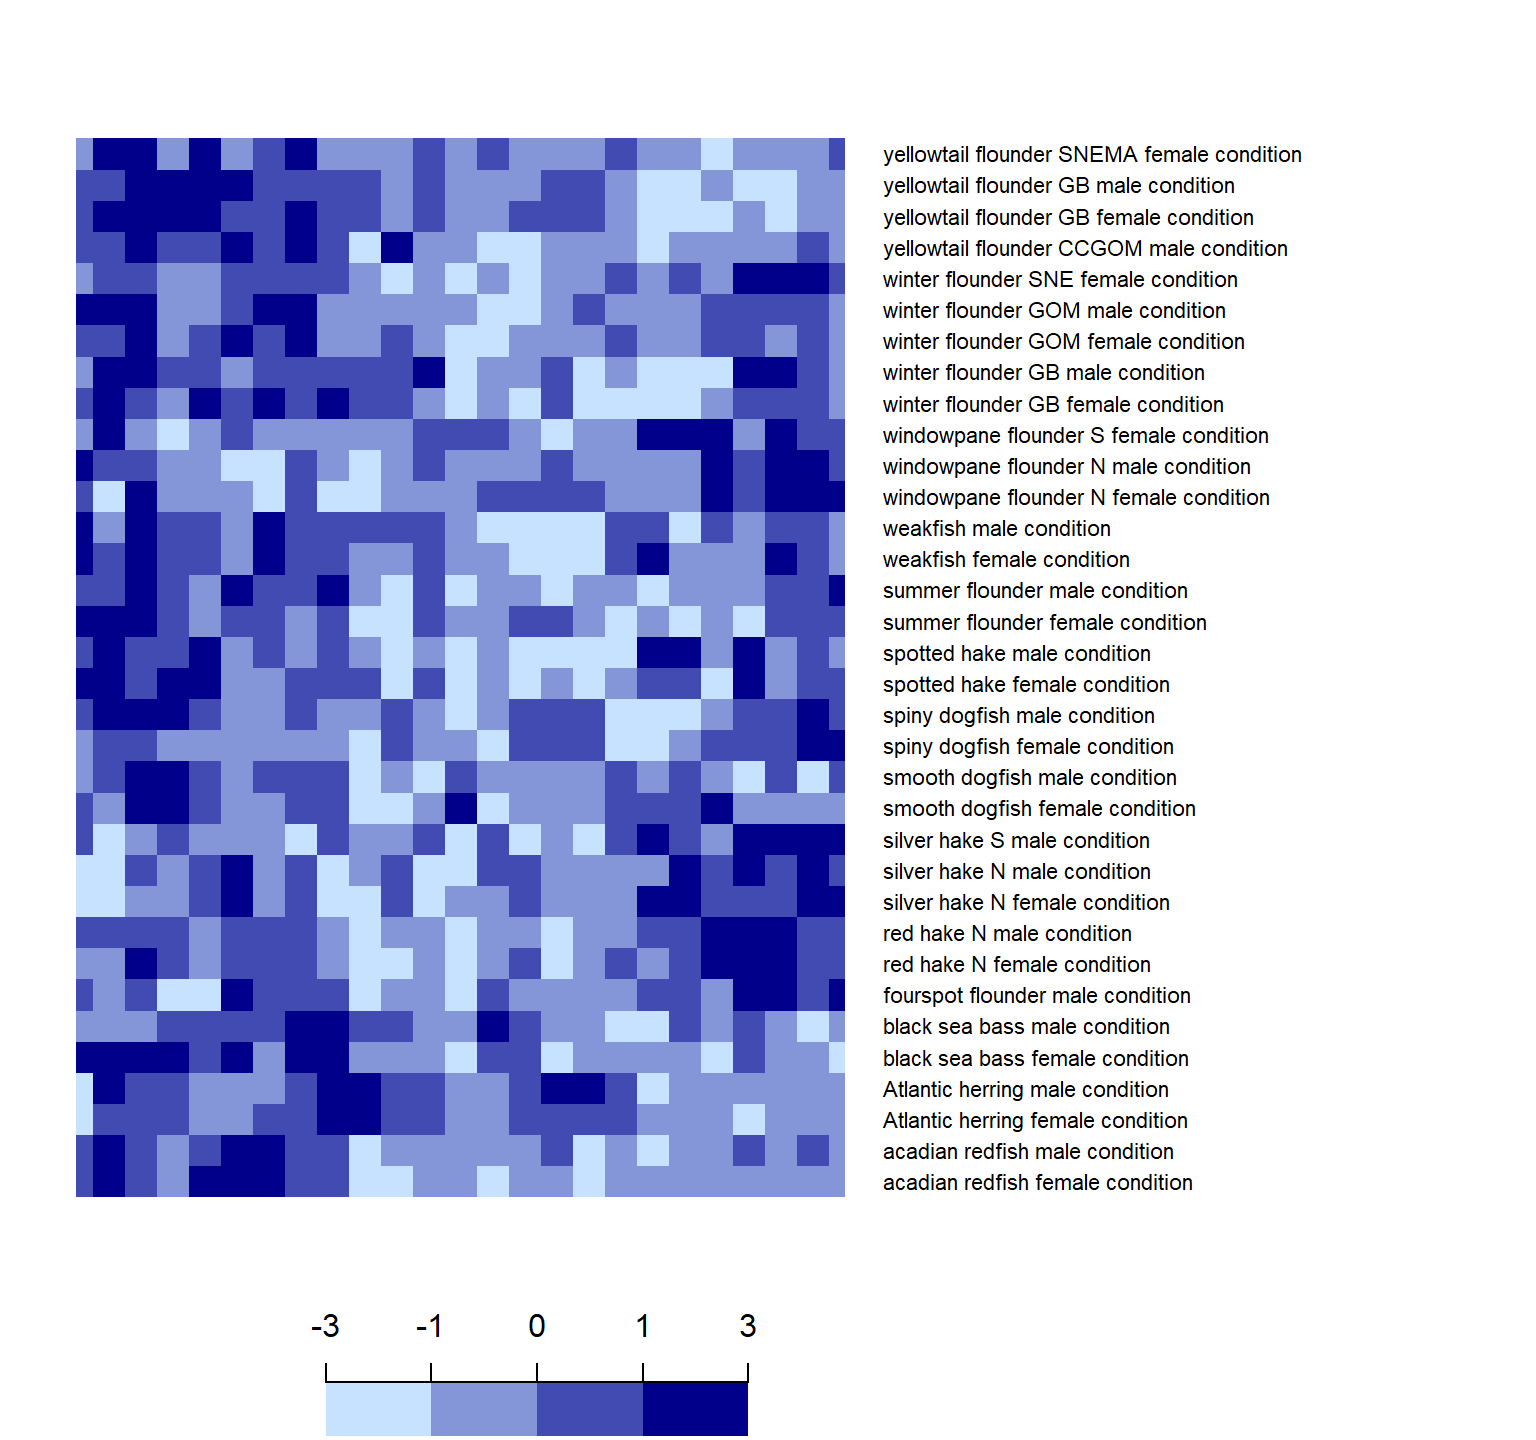
\includegraphics{C:/Users/kimberly.bastille/Desktop/tech-doc/imagescondition-factor-1.pdf}
\caption{\label{fig:condition-factor}Normalized condition factors of managed
species in the Northeast Large Marine Ecosystem.}
\end{figure}

\hypertarget{epu}{\chapter{Ecological Production Units}\label{epu}}

\textbf{Description}: Ecological Production Units

\textbf{Found in}: State of the Ecosystem - Gulf of Maine \& Georges
Bank (2018, 2019), State of the Ecosystem - Mid-Atlantic (2018, 2019)

\textbf{Indicator category}: Extensive analysis, not yet published

\textbf{Contributor(s)}: Robert Gamble

\textbf{Data steward}: NA

\textbf{Point of contact}: Robert Gamble,
\href{mailto:robert.gamble@noaa.gov}{\nolinkurl{robert.gamble@noaa.gov}}

\textbf{Public availability statement}: Ecological production unit (EPU)
shapefiles are available
\href{https://github.com/NOAA-EDAB/tech-doc/tree/master/gis}{here}. More
information about source data used to derive EPUs can be found
\href{https://www.integratedecosystemassessment.noaa.gov/sites/default/files/pdf/ne-ecological-production-units-paper.pdf}{here}.

\section{Methods}\label{methods-11}

To define ecological production units, we assembled a set of
physiographic, oceanographic and biotic variables on the Northeast U.S.
Continental Shelf, an area of approximately 264,000 km within the 200 m
isobath. The physiographic and hydrographic variables selected have been
extensively used in previous analyses of oceanic provinces and regions
(e.g Roff and Taylor \protect\hyperlink{ref-Roff2000}{2000}). Primary
production estimates have also been widely employed for this purpose in
conjunction with physical variables (Longhurst
\protect\hyperlink{ref-Longhurst2007}{2007}) to define ecological
provinces throughout the world ocean.

We did not include information on zooplankton, benthic invertebrates,
fish, protected species, or fishing patterns in our analysis. The
biomass and production of the higher trophic level groups in this region
has been sharply perturbed by fishing and other anthropogenic
influences. Similarly, fishing patterns are affected by regulatory
change, market and economic factors and other external influences.

Because these malleable patterns of change are often unconnected with
underlying productivity, we excluded factors directly related to fishing
practices. The physiographic variables considered in this analysis are
listed in Table \ref{tab:epuinputs}. They include bathymetry and
surficial sediments. The physical oceanographic and hydrographic
measurements include sea surface temperature, annual temperature span,
and temperature gradient water derived from satellite observations for
the period 1998 to 2007.

\subsection{Data sources}\label{data-sources-11}

Shipboard observations for surface and bottom water temperature and
salinity in surveys conducted in spring and fall. Daily sea surface
temperature (SST, °C) measurements at 4 km resolution were derived from
nighttime scenes composited from the AVHRR sensor on NOAA's
polar-orbiting satellites and from NASA's MODIS TERRA and MODIS AQUA
sensors. We extracted information for the annual mean SST, temperature
span, and temperature gradients from these sources. The latter metric
provides information on frontal zone locations.

\begin{table}

\caption{\label{tab:epuinputs}Variables used in derivation of Ecological Production Units.}
\centering
\begin{tabular}[t]{lll}
\toprule
Variables & Sampling Method & Units\\
\midrule
Surficial Sediments & Benthic Grab & Krumbian Scale\\
Sea Surface Temperature & Satellite Imagery (4km grid) & \&deg;C annual average\\
Sea Surface Temperature & Satellite Imagery (4km grid) & dimensionless\\
Sea Surface Temperature & Satellite Imagery (4km grid) & \&deg;C annual average\\
Surface Temperature & Shipboard hydrography (point) & \&deg;C (Spring and Fall)\\
\addlinespace
Bottom Temperature & Shipboard hydrography (point) & \&deg;C (Spring and Fall)\\
Surface Salinity & Shipboard hydrography (point) & psu (Spring and Fall)\\
Bottom Salinity & Shipboard hydrography (point) & psu (Spring and Fall)\\
Stratification & Shipboard hydrography (point) & Sigma-t units (Spring and Fall)\\
Chlorophyll-a & Satellite Imagery (1.25 km grid) & mg/C/m\textasciicircum{}3\textasciicircum{} (annual average)\\
\addlinespace
Chlorophyll-a gradient & Satellite Imagery (1.25 km grid) & dimensionless\\
Chlorophyll-a span & Satellite Imagery (1.25 km grid) & mg/C/m\textasciicircum{}3\textasciicircum{} (annual average)\\
Primary Production & Satellite Imagery (1.25 km grid) & gC/m\textasciicircum{}3\textasciicircum{}/year (cumulative)\\
Primary Production gradient & Satellite Imagery (1.25 km grid) & dimensionless\\
Primary Production span & Satellite Imagery (1.25 km grid) & gC/m\textasciicircum{}3\textasciicircum{}/year (cumulative)\\
\bottomrule
\end{tabular}
\end{table}

The biotic measurements included satellite-derived estimates of
chlorophyll \emph{a} (CHLa) mean concentration, annual span, and CHLa
gradients and related measures of primary production. Daily merged
SeaWiFS/MODIS-Aqua CHLa (CHL, mg m\textsuperscript{-3}) and SeaiWiFS
photosynthetically available radiation (PAR, Einsteins
m\textsuperscript{-2} d\textsuperscript{-1}) scenes at 1.25 km
resolution were obtained from NASA Ocean Biology Processing Group.

\subsection{Data extraction}\label{data-extraction-10}

NA

\subsection{Data analysis}\label{data-analysis-10}

In all cases, we standardized the data to common spatial units by taking
annual means of each observation type within spatial units of 10'
latitude by 10' longitude to account for the disparate spatial and
temporal scales at which these observations are taken. There are over
1000 spatial cells in this analysis. Shipboard sampling used to obtain
direct hydrographic measurements is constrained by a minimum sampling
depth of 27 m specified on the basis of prescribed safe operating
procedures. As a result nearshore waters are not fully represented in
our initial specifications of ecological production units.

The size of the spatial units employed further reflects a compromise
between retaining spatial detail and minimizing the need for spatial
interpolation of some data sets. For shipboard data sets characterized
by relatively coarse spatial resolution, where necessary, we first
constructed an interpolated map using an inverse distance weighting
function before including it in the analysis. Although alternative
interpolation schemes based on geostatistical approaches are possible,
we considered the inverse distance weighting function to be both
tractable and robust for this application.

We first employed a spatial principal components analysis (PCA; e.g.
Pielou \protect\hyperlink{ref-Pielou1984}{1984}; Legendre and Legendre
\protect\hyperlink{ref-Legendre1998}{1998}) to examine the multivariate
structure of the data and to account for any inter-correlations among
the variables to be used in subsequent analysis. The variables included
in the analysis exhibited generally skewed distributions and we
therefore transformed each to natural logarithms prior to analysis.

The PCA was performed on the correlation matrix of the transformed
observations. We selected the eigenvectors associated with eigenvalues
of the dispersion matrix with scores greater than 1.0 (the
Kaiser-Guttman criterion; Legendre and Legendre
\protect\hyperlink{ref-Legendre1998}{1998}) for all subsequent analysis.
These eigenvectors represent orthogonal linear combinations of the
original variables used in the analysis.

We delineated ecological subunits by applying a disjoint cluster based
on Euclidean distances using the K-means procedure (Legendre and
Legendre \protect\hyperlink{ref-Legendre1998}{1998}) on the principal
component scores The use of non-independent variables can strongly
influence the results of classification analyses of this type (Pielou
\protect\hyperlink{ref-Pielou1984}{1984}), hence the interest in using
the PCA results in the cluster.

The eigenvectors were represented as standard normal deviates. We used a
Pseudo-F Statistic described by Milligan and Cooper
(\protect\hyperlink{ref-Milligan1985}{1985}) to objectively define the
number of clusters to use in the analysis. The general approach employed
is similar to that of Host et al.
(\protect\hyperlink{ref-Host1996}{1996}) for the development of regional
ecosystem classifications for terrestrial systems.

After the analyses were done, we next considered options for
interpolation of nearshore boundaries resulting from depth-related
constraints on shipboard observations. For this, we relied on
information from satellite imagery. For the missing nearshore areas in
the Gulf of Maine and Mid-Atlantic Bight, the satellite information for
chlorophyll concentration and sea surface temperature indicated a direct
extension from adjacent observations. For the Nantucket Shoals region
south of Cape Cod, similarities in tidal mixing patterns reflected in
chlorophyll and temperature observations indicated an affinity with
Georges Bank and the boundaries were changed accordingly.

Finally, we next considered consolidation of ecological subareas so that
nearshore regions are considered to be special zones nested within the
adjacent shelf regions. Similar consideration led to nesting the
continental slope regions within adjacent shelf regions in the
Mid-Atlantic and Georges Bank regions. This led to four major units:
Mid-Atlantic Bight, Georges Bank, Western-Central Gulf of Maine (simply
``Gulf of Maine'' in the SOE), and Scotian Shelf-Eastern Gulf of Maine.
As the State of the Ecosystem reports are specific to FMC managed
regions, the Scotian Shelf-Eastern Gulf of Maine EPU is not considered
in SOE indicator analyses.

\begin{figure}

{\centering 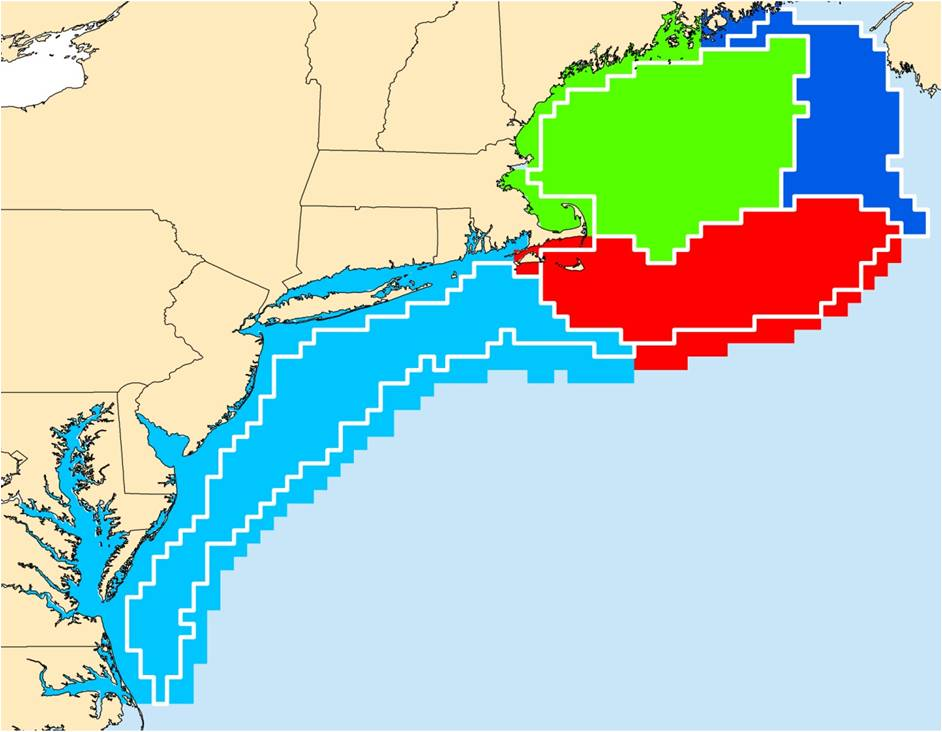
\includegraphics{C:/Users/kimberly.bastille/Desktop/tech-doc/images/EPUs} 

}

\caption{Map of the four Ecological Production Units, including the Mid-Atlantic Bight (light blue), Georges Bank (red), Western-Central Gulf of Maine (or Gulf of Maine; green), and Scotian Shelf-Eastern Gulf of Maine (dark blue)}\label{fig:EPUmap}
\end{figure}

\subsection{Data processing}\label{data-processing-6}

Shapefiles were converted to \texttt{sf} objects for inclusion in the
ecodata R package using the following R code.

\begin{Shaded}
\begin{Highlighting}[]
\CommentTok{# A function to process and make ecological production unit (EPU) shapefiles available in the ecodata package. }

\CommentTok{# Read more about the delineation of EPUs at https://noaa-edab.github.io/tech-doc/epu.html}


\KeywordTok{library}\NormalTok{(sf)}
\KeywordTok{library}\NormalTok{(rgdal)}
\KeywordTok{library}\NormalTok{(raster)}
\KeywordTok{library}\NormalTok{(rnaturalearth)}



\NormalTok{gis.dir <-}\StringTok{ }\NormalTok{here}\OperatorTok{::}\KeywordTok{here}\NormalTok{(}\StringTok{'inst'}\NormalTok{,}\StringTok{'extdata'}\NormalTok{,}\StringTok{'gis'}\NormalTok{)}
\NormalTok{crs <-}\StringTok{ "+proj=longlat +lat_1=35 +lat_2=45 +lat_0=40 +lon_0=-77+x_0=0}
\StringTok{+y_0=0 +datum=NAD83 +no_defs +ellps=GRS80 +towgs84=0,0,0"}

\NormalTok{get_epu_sf <-}\StringTok{ }\ControlFlowTok{function}\NormalTok{(save_clean)\{}
  
\NormalTok{  epu_shp <-}\StringTok{ }\KeywordTok{readOGR}\NormalTok{(}\KeywordTok{file.path}\NormalTok{(gis.dir, }\StringTok{"EPU_Extended.shp"}\NormalTok{), }\DataTypeTok{verbose =}\NormalTok{ F) }
  \KeywordTok{crs}\NormalTok{(epu_shp) <-}\StringTok{ }\NormalTok{crs}
\NormalTok{  epu_sf <-}\StringTok{ }\KeywordTok{as}\NormalTok{(epu_shp, }\StringTok{"sf"}\NormalTok{)}
  
  \ControlFlowTok{if}\NormalTok{ (save_clean)\{}
\NormalTok{    usethis}\OperatorTok{::}\KeywordTok{use_data}\NormalTok{(epu_sf)}
\NormalTok{  \} }\ControlFlowTok{else}\NormalTok{ \{}
    \KeywordTok{return}\NormalTok{(epu_sf)}
\NormalTok{  \}}
\NormalTok{\}}
\end{Highlighting}
\end{Shaded}

\chapter{Gulf Stream Index}\label{gulf-stream-index}

\textbf{Description}: Annual time series of the Gulf Stream index

\textbf{Indicator category}: Published method

\textbf{Found in}: State of the Ecosystem - New England (2019)

\textbf{Contributor(s)}: Terry Joyce, Rong Zhang

\textbf{Data steward}: Vincent Saba,
\href{mailto:vincent.saba@noaa.gov}{\nolinkurl{vincent.saba@noaa.gov}}

\textbf{Point of contact}: Vincent Saba,
\href{mailto:vincent.saba@noaa.gov}{\nolinkurl{vincent.saba@noaa.gov}}

\textbf{Public availability statement}: Source data are publicly
available

\section{Methods}\label{methods-12}

Summarized from Joyce et al. (\protect\hyperlink{ref-joyce2019}{2019}),
ocean temperature data from NOAA's National Centers for Environmental
Information (NCEI) were sorted by latitude, longitude, and time using a
resolution of 1\textdegree of longitude, latitude, and 3 months of time,
respectively, with a Gaussian squared weighting from the selected
desired point in a window twice the size of the desired resolution.
Editing was used to reject duplicate samples and 3\(\sigma\) outliers
from each selected sample point prior to performing the weighting and
averaging; the latter was only carried out when there were at least
three data points in the selected interval for each sample point.
Typically, 50 or more data values were available. The resulting
temperature field was therefore smoothed. Data along the Gulf Stream
north wall at nine data points were used to assemble a spatial/temporal
sampling of the temperature at 200m data along the north wall from
75\textdegree W to 55\textdegree W. The leading mode of temperature
variability of the Gulf Stream is equivalent to a north‐south shift of
50--100 km, which is zonally of one sign and amounts to 50\% of the
seasonal‐interannual variance between 75\textdegree W and
55\textdegree W. The temporal behavior of this mode (PC1) shows the
temporal shift of the Gulf Stream path with a dominant approximately 8‐
to 10‐year periodicity over much of the period.

\subsection{Data sources}\label{data-sources-12}

Ocean temperatures at 200 m are available at
\url{https://www.nodc.noaa.gov/OC5/3M_HEAT_CONTENT/}.

\subsection{Data analysis}\label{data-analysis-11}

For detailed analytical methods, see Joyce et al.
(\protect\hyperlink{ref-joyce2019}{2019}).

\subsection{Data Processing}\label{data-processing-7}

The Gulf Stream index data set was formatted for inclusion in the
ecodata R package with the following code.

\begin{Shaded}
\begin{Highlighting}[]
\CommentTok{# Processing for Gulf Stream Index data}

\CommentTok{# GSI = degrees latitude above the average Gulf Stream position based}
\CommentTok{# on ocean temperature at 200m (15 C) depth between 55W to 75W.}

\KeywordTok{library}\NormalTok{(dplyr)}
\KeywordTok{library}\NormalTok{(tidyr)}
\KeywordTok{library}\NormalTok{(lubridate)}

\NormalTok{raw.dir <-}\StringTok{ }\NormalTok{here}\OperatorTok{::}\KeywordTok{here}\NormalTok{(}\StringTok{"data-raw"}\NormalTok{)}

\NormalTok{get_gsi <-}\StringTok{ }\ControlFlowTok{function}\NormalTok{(}\DataTypeTok{save_clean =}\NormalTok{ F)\{}

\NormalTok{  gsi <-}\StringTok{ }\KeywordTok{read.csv}\NormalTok{(}\KeywordTok{file.path}\NormalTok{(raw.dir, }\StringTok{"GSI.csv"}\NormalTok{)) }\OperatorTok\StringTok{ }
\StringTok{    }\NormalTok{dplyr}\OperatorTok{::}\KeywordTok{rename}\NormalTok{(}\DataTypeTok{Time =}\NormalTok{ Year, }\DataTypeTok{Value =}\NormalTok{ GSI) }\OperatorTok\StringTok{ }
\StringTok{    }\KeywordTok{mutate}\NormalTok{(}\DataTypeTok{Var =} \StringTok{"gulf stream index"}\NormalTok{,}
           \DataTypeTok{Units =} \StringTok{"latitude anomaly"}\NormalTok{,}
           \DataTypeTok{EPU =} \StringTok{"All"}\NormalTok{)}
  
  \ControlFlowTok{if}\NormalTok{ (save_clean)\{}
\NormalTok{    usethis}\OperatorTok{::}\KeywordTok{use_data}\NormalTok{(gsi, }\DataTypeTok{overwrite =}\NormalTok{ T)}
\NormalTok{  \} }\ControlFlowTok{else}\NormalTok{ \{}
    \KeywordTok{return}\NormalTok{(gsi)}
\NormalTok{  \}}
\NormalTok{\}}
\end{Highlighting}
\end{Shaded}

\chapter{Harbor Porpoise Bycatch}\label{harbor-porpoise-bycatch}

\textbf{Description}: Harbor Porpoise Indicator

\textbf{Found in}: State of the Ecosystem - Gulf of Maine \& Georges
Bank (2018, 2019), State of the Ecosystem - Mid-Atlantic (2018, 2019)

\textbf{Indicator category}: Synthesis of published information;
Published methods

\textbf{Contributor(s)}: Christopher D. Orphandies

\textbf{Data steward}: Chris Orphanides,
\href{mailto:chris.orphanides@noaa.gov}{\nolinkurl{chris.orphanides@noaa.gov}}

\textbf{Point of contact}: Chris Orphanides,
\href{mailto:chris.orphanides@noaa.gov}{\nolinkurl{chris.orphanides@noaa.gov}}

\textbf{Public availability statement}: Source data are available in
public
\href{https://www.fisheries.noaa.gov/national/marine-mammal-protection/marine-mammal-stock-assessment-reports-region}{stock
assessment reports} (2018 report in-press). Derived data as shown in the
2018 SOE reports are available
\href{http://comet.nefsc.noaa.gov/erddap/tabledap/protected_species_soe_v1.html}{here}

\section{Methods}\label{methods-13}

\subsection{Data sources}\label{data-sources-13}

Reported harbor porpoise bycatch estimates and potential biological
removal levels can be found in publicly available documents; detailed
\href{https://www.fisheries.noaa.gov/national/marine-mammal-protection/marine-mammal-stock-assessment-reports-region}{here}.
The most recent bycatch estimates for 2016 were taken from the 2018
stock assessment (in-press). More detailed documentation as to the
methods employed can be found in NOAA Fisheries Northeast Fisheries
Science Center (NEFSC) Center Reference Documents (CRDs) found on the
NEFSC \href{https://www.nefsc.noaa.gov/publications/crd/}{publications
page}.

The document for the 2016 estimates (CRD 19-04) is available
\href{https://www.nefsc.noaa.gov/publications/crd/crd1904/crd1904.pdf}{here}.
Additional methodological details are available for previous year's
estimates and are documented in numerous published CRDs:
\href{https://www.nefsc.noaa.gov/publications/crd/crd1718/crd1718.pdf}{CRD
17-18},
\href{https://www.nefsc.noaa.gov/publications/crd/crd1605/crd1605.pdf}{CRD-16-05},
\href{https://www.nefsc.noaa.gov/publications/crd/crd1515/crd1515.pdf}{CRD
15-15}, \href{https://repository.library.noaa.gov/view/noaa/4718}{CRD
14-02},
\href{https://www.nefsc.noaa.gov/publications/crd/crd1313/crd1313_2nd_ed.pdf}{CRD
13-13},
\href{https://www.nefsc.noaa.gov/publications/crd/crd1108/1108.pdf}{CRD
11-08},
\href{https://www.nefsc.noaa.gov/publications/crd/crd1010/crd1010.pdf}{CRD
10-10},
\href{https://www.nefsc.noaa.gov/publications/crd/crd0720/crd0720.pdf}{CRD
07-20},
\href{https://www.nefsc.noaa.gov/publications/crd/crd0613/crd0613.pdf}{CRD
06-13},
\href{https://www.nefsc.noaa.gov/publications/crd/crd0318/crd0318.pdf}{CRD
03-18},
\href{https://www.nefsc.noaa.gov/publications/crd/crd0115/0115.pdf}{CRD
01-15}, and
\href{https://www.nefsc.noaa.gov/publications/crd/pdfs/crd9917.pdf}{CRD
99-17}.

\subsection{Data extraction}\label{data-extraction-11}

Annual gillnet bycatch estimates are documented in a CRD (see sources
above). These feed into the Stock Assessment Reports which report both
the annual bycatch estimate and the mean 5-year estimate. The 5-year
estimate is the one used for management purposes, so that is the one
provided for the SOE plot.

\subsection{Data analysis}\label{data-analysis-12}

Bycatch estimates as found in stock assessment reports were plotted
along with confidence intervals. The confidence intervals were
calculated from published CVs assuming a normal distribution
(\(\sigma = \mu CV\); \(CI = \bar{x} \pm \sigma * 1.96\)).

Data were analyzed and formatted for inclusion in the ecodata R package
using the following R code.

\begin{Shaded}
\begin{Highlighting}[]
\CommentTok{# Process harbor porpoise bycatch estimates}

\CommentTok{# Time series figure is 5-yr running mean for harbor porpoise bycatch estimates for the Northeast US across all fisheries.}

\KeywordTok{library}\NormalTok{(dplyr)}
\KeywordTok{library}\NormalTok{(tidyr)}

\NormalTok{raw.dir <-}\StringTok{ }\NormalTok{here}\OperatorTok{::}\KeywordTok{here}\NormalTok{(}\StringTok{"data-raw"}\NormalTok{)}

\CommentTok{#HP bycatch time series estimates------------------------------------------------------}
\NormalTok{get_harborporpoise <-}\StringTok{ }\ControlFlowTok{function}\NormalTok{(}\DataTypeTok{save_clean =}\NormalTok{ F)\{}
\NormalTok{  d <-}\StringTok{ }\KeywordTok{read.csv}\NormalTok{(}\KeywordTok{file.path}\NormalTok{(raw.dir,}\StringTok{"1994-2017_5yr_hp_est.csv"}\NormalTok{))}
  
  \CommentTok{#Create confidence intervals}
\NormalTok{  var1nnum <-}\StringTok{ }\KeywordTok{log}\NormalTok{(}\DecValTok{1}\OperatorTok{+}\NormalTok{d}\OperatorTok{$}\NormalTok{CV}\OperatorTok{^}\DecValTok{2}\NormalTok{)  }
\NormalTok{  c <-}\StringTok{ }\KeywordTok{exp}\NormalTok{(}\FloatTok{1.96} \OperatorTok{*}\StringTok{ }\KeywordTok{sqrt}\NormalTok{(var1nnum))}
\NormalTok{  d}\OperatorTok{$}\NormalTok{up95ci <-}\StringTok{ }\NormalTok{d}\OperatorTok{$}\NormalTok{EST }\OperatorTok{*}\StringTok{ }\NormalTok{c}
\NormalTok{  d}\OperatorTok{$}\NormalTok{lo95ci <-}\StringTok{ }\NormalTok{d}\OperatorTok{$}\NormalTok{EST }\OperatorTok{/}\StringTok{ }\NormalTok{c}
  
  
\NormalTok{  harborporpoise <-}\StringTok{ }\NormalTok{d }\OperatorTok\StringTok{ }\NormalTok{dplyr}\OperatorTok{::}\KeywordTok{rename}\NormalTok{(}\DataTypeTok{Time =}\NormalTok{ YEAR) }\OperatorTok\StringTok{ }
\StringTok{    }\KeywordTok{gather}\NormalTok{(., Var, Value, }\OperatorTok{-}\NormalTok{Time) }\OperatorTok\StringTok{ }
\StringTok{    }\KeywordTok{mutate}\NormalTok{(}\DataTypeTok{Units =} \StringTok{"N"}\NormalTok{,}
           \DataTypeTok{EPU =} \StringTok{"All"}\NormalTok{,}
\NormalTok{           Var, }\DataTypeTok{Var =}\NormalTok{ plyr}\OperatorTok{::}\KeywordTok{mapvalues}\NormalTok{(Var, }\DataTypeTok{from =} \KeywordTok{c}\NormalTok{(}\StringTok{"EST"}\NormalTok{,}\StringTok{"CV"}\NormalTok{,}\StringTok{"PBR"}\NormalTok{,}\StringTok{"up95ci"}\NormalTok{,}\StringTok{"lo95ci"}\NormalTok{),}
                                      \DataTypeTok{to =} \KeywordTok{c}\NormalTok{(}\StringTok{"harbor porpoise bycatch estimate"}\NormalTok{,}
                                             \StringTok{"harbor porpoise bycatch cv"}\NormalTok{,}
                                             \StringTok{"harbor porpoise bycatch pbr"}\NormalTok{,}
                                             \StringTok{"harbor porpoise bycatch up95ci"}\NormalTok{,}
                                             \StringTok{"harbor porpoise bycatch lo95ci"}\NormalTok{))) }\OperatorTok\StringTok{ }
\StringTok{    }\KeywordTok{as.data.frame}\NormalTok{()}
  
  \ControlFlowTok{if}\NormalTok{ (save_clean)\{}
\NormalTok{    usethis}\OperatorTok{::}\KeywordTok{use_data}\NormalTok{(harborporpoise, }\DataTypeTok{overwrite =}\NormalTok{ R)}
\NormalTok{  \} }\ControlFlowTok{else}\NormalTok{ \{}
    \KeywordTok{return}\NormalTok{(harborporpoise)}
\NormalTok{  \}}
\NormalTok{\}}
\end{Highlighting}
\end{Shaded}

\subsection{Plotting}\label{plotting-8}

\begin{Shaded}
\begin{Highlighting}[]
\CommentTok{# Relative working directories}
\NormalTok{data.dir  <-}\StringTok{ }\NormalTok{here}\OperatorTok{::}\KeywordTok{here}\NormalTok{(}\StringTok{'data'}\NormalTok{)}
\NormalTok{r.dir <-}\StringTok{ }\NormalTok{here}\OperatorTok{::}\KeywordTok{here}\NormalTok{(}\StringTok{'R'}\NormalTok{)}

\CommentTok{# Load data}
\KeywordTok{load}\NormalTok{(}\KeywordTok{file.path}\NormalTok{(data.dir,}\StringTok{"SOE_data_erddap.Rdata"}\NormalTok{))}

\CommentTok{# Source plotting functions}
\KeywordTok{source}\NormalTok{(}\KeywordTok{file.path}\NormalTok{(r.dir,}\StringTok{"BasePlot_source.R"}\NormalTok{))}


\NormalTok{opar <-}\StringTok{ }\KeywordTok{par}\NormalTok{(}\DataTypeTok{mar =} \KeywordTok{c}\NormalTok{(}\DecValTok{4}\NormalTok{, }\DecValTok{6}\NormalTok{, }\DecValTok{2}\NormalTok{, }\DecValTok{6}\NormalTok{))}

\KeywordTok{soe.plot}\NormalTok{(SOE.data, }\StringTok{'Time'}\NormalTok{, }\StringTok{"Harbor porpoise bycatch estimates"}\NormalTok{,            }
         \DataTypeTok{rel.y.num =} \FloatTok{1.2}\NormalTok{, }\DataTypeTok{end.start =} \DecValTok{2007}\NormalTok{, }\DataTypeTok{full.trend =}\NormalTok{ F, }\DataTypeTok{point.cex =} \DecValTok{1}\NormalTok{,}
         \DataTypeTok{ymax =}\NormalTok{ F, }\DataTypeTok{y.upper =} \DecValTok{2500}\NormalTok{, }\DataTypeTok{mean_line =}\NormalTok{ F, }\DataTypeTok{x.label =} \StringTok{'Year'}\NormalTok{,}
         \DataTypeTok{y.label =} \StringTok{'Bycatch, n'}\NormalTok{, }\DataTypeTok{rel.y.text =} \DecValTok{1}\NormalTok{)}

\KeywordTok{legend}\NormalTok{(}\DecValTok{2000}\NormalTok{, }\DecValTok{2250}\NormalTok{, }\DataTypeTok{legend =} \StringTok{"Potential Biological Removal"}\NormalTok{,}
       \DataTypeTok{col =} \KeywordTok{adjustcolor}\NormalTok{(}\StringTok{"red"}\NormalTok{, .}\DecValTok{5}\NormalTok{), }\DataTypeTok{lwd =} \DecValTok{3}\NormalTok{,}
       \DataTypeTok{bty =} \StringTok{"n"}\NormalTok{, }\DataTypeTok{cex =} \FloatTok{0.9}\NormalTok{)}

\CommentTok{#credible intervals and PBI}
\NormalTok{lw_CI <-}\StringTok{ }\NormalTok{SOE.data[Var }\OperatorTok{==}\StringTok{ 'Harbor porpoise bycatch 2.5 CI'}\NormalTok{,}
                       \KeywordTok{list}\NormalTok{(Time, Value)]}
\NormalTok{up_CI <-}\StringTok{ }\NormalTok{SOE.data[Var }\OperatorTok{==}\StringTok{ 'Harbor porpoise bycatch 97.5 CI'}\NormalTok{,}
                       \KeywordTok{list}\NormalTok{(Time, Value)]}
\NormalTok{pbi   <-}\StringTok{ }\NormalTok{SOE.data[Var }\OperatorTok{==}\StringTok{ 'Harbor porpoise potential biological removal'}\NormalTok{,}
                       \KeywordTok{list}\NormalTok{(Time, Value)]}

\KeywordTok{points}\NormalTok{(pbi,   }\DataTypeTok{type  =} \StringTok{"l"}\NormalTok{, }\DataTypeTok{lty =} \DecValTok{1}\NormalTok{, }\DataTypeTok{col =} \KeywordTok{adjustcolor}\NormalTok{(}\StringTok{"red"}\NormalTok{, .}\DecValTok{5}\NormalTok{), }\DataTypeTok{lwd =} \DecValTok{3}\NormalTok{)}
\KeywordTok{points}\NormalTok{(lw_CI, }\DataTypeTok{type  =} \StringTok{"l"}\NormalTok{, }\DataTypeTok{lty =} \DecValTok{2}\NormalTok{, }\DataTypeTok{col =} \KeywordTok{adjustcolor}\NormalTok{(}\StringTok{"darkorange"}\NormalTok{, .}\DecValTok{9}\NormalTok{), }\DataTypeTok{lwd =} \FloatTok{2.5}\NormalTok{)}
\KeywordTok{points}\NormalTok{(up_CI, }\DataTypeTok{type  =} \StringTok{"l"}\NormalTok{, }\DataTypeTok{lty =} \DecValTok{2}\NormalTok{, }\DataTypeTok{col =} \KeywordTok{adjustcolor}\NormalTok{(}\StringTok{"darkorange"}\NormalTok{, .}\DecValTok{9}\NormalTok{), }\DataTypeTok{lwd =} \FloatTok{2.5}\NormalTok{)}
\end{Highlighting}
\end{Shaded}

\begin{figure}
\centering
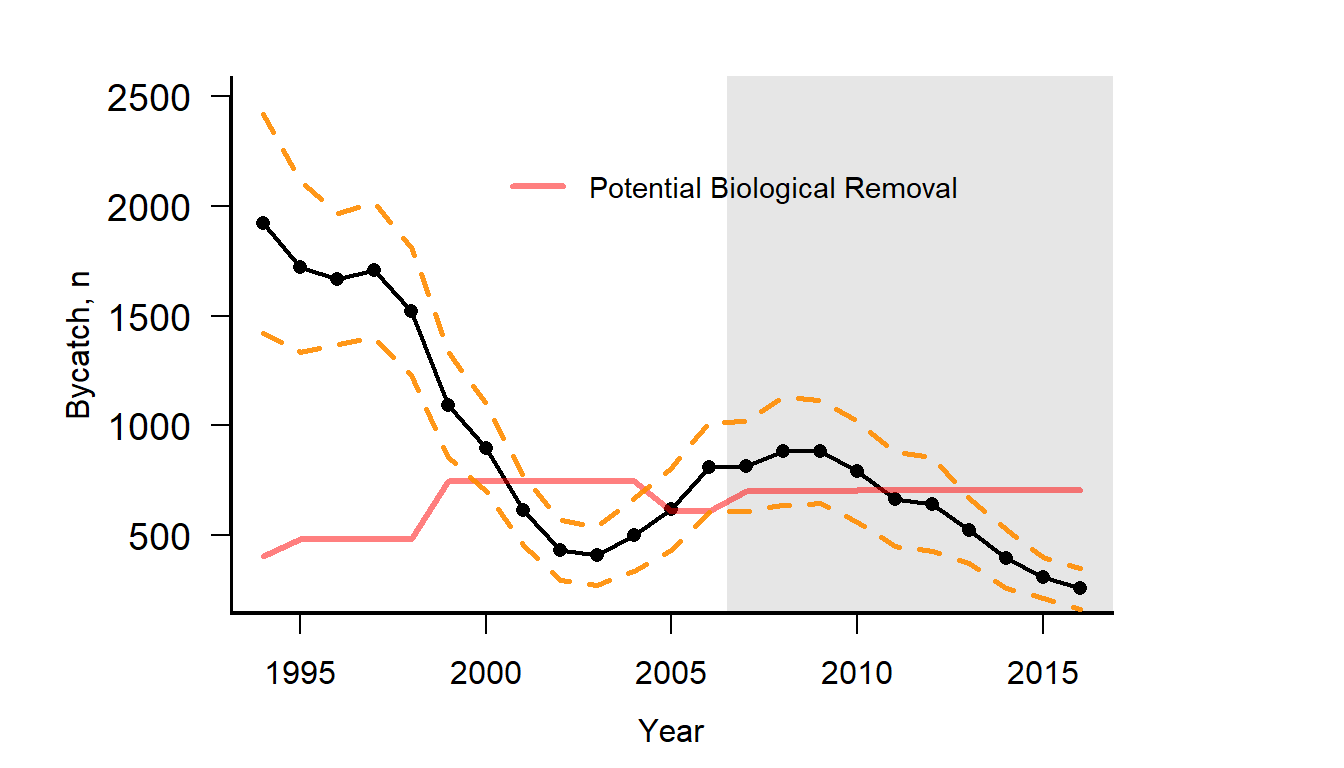
\includegraphics{C:/Users/kimberly.bastille/Desktop/tech-doc/imagesharbor-porpoise-1.pdf}
\caption{\label{fig:harbor-porpoise}Harbor porpoise bycatch estimated shown
with Potential Biological Removal (red) and confidence intervals
(orange).}
\end{figure}

\chapter{Ichthyoplankton Diversity}\label{ichthyoplankton-diversity}

\textbf{Description}: NOAA NEFSC Oceans and Climate branch public
ichthyoplankton dataset

\textbf{Found in}: State of the Ecosystem - Gulf of Maine \& Georges
Bank (2018, 2019), State of the Ecosystem - Mid-Atlantic (2018, 2019)

\textbf{Indicator category}: Database pull with analysis

\textbf{Contributor(s)}: Harvey J. Walsh

\textbf{Data steward}: Harvey Walsh,
\href{mailto:harvey.walsh@noaa.gov}{\nolinkurl{harvey.walsh@noaa.gov}}

\textbf{Point of contact}: Harvey Walsh,
\href{mailto:harvey.walsh@noaa.gov}{\nolinkurl{harvey.walsh@noaa.gov}}

\textbf{Public availability statement}: Source data are available to the
public
\href{ftp://ftp.nefsc.noaa.gov/pub/hydro/zooplankton_data/}{here}.
Derived data for this indicator are available
\href{https://comet.nefsc.noaa.gov/erddap/tabledap/ichthyo_div_soe_v1.html}{here}.

\section{Methods}\label{methods-14}

Data from the NOAA NEFSC Oceans and Climate branch public dataset were
used to examine changes in diversity of abundance among 45
ichthyoplankton taxa. The 45 taxa were established (Walsh et al.
\protect\hyperlink{ref-RN126}{2015}), and include the most abundant taxa
from the 1970s to present that represent consistency in the
identification of larvae.

\subsection{Data sources}\label{data-sources-14}

Multi-species plankton surveys cover the entire Northeast US shelf from
Cape Hatteras, North Carolina, to Cape Sable, Nova Scotia, four to six
times per year. A random-stratified design based on the NEFSC bottom
trawl survey design (Azarovitz
\protect\hyperlink{ref-Azarovitz1981}{1981}) is used to collect samples
from 47 strata. The number of strata is lower than the trawl survey as
many of the narrow inshore and shelf-break strata are combined in the
EcoMon design. The area encompassed by each stratum determined the
number of samples in each stratum. Samples were collected both day and
night using a 61 cm bongo net. Net tow speed was 1.5 knots and maximum
sample depth was 200 m. Double oblique tows were a minimum of 5 mintues
in duration, and fished from the surface to within 5 m of the seabed or
to a maximum depth of 200 m. The volume filtered of all collections was
measured with mechanical flowmeters mounted across the mouth of each
net.

Processing of most samples was conducted at the Morski Instytut Rybacki
(MIR) in Szczecin, Poland; the remaining samples were processed at the
NEFSC or the Atlantic Reference Center, St Andrews, Canada. Larvae were
identified to the lowest possible taxa and enumerated for each sample.
Taxon abundance for each station was standardized to number under 10
m\textsuperscript{-2} sea surface.

\subsection{Data extraction}\label{data-extraction-12}

Data retrieved from NOAA NEFSC Oceans and Climate branch
\href{ftp://ftp.nefsc.noaa.gov/pub/hydro/zooplankton_data/}{public
dataset} (Filename: ``EcoMon\_Plankton\_Data\_v3\_0.xlsx'', File Date:
10/20/2016).

\subsection{Data analysis}\label{data-analysis-13}

All detailed data processing steps are not currently included in this
document, but general steps are outlined. Data were grouped into
seasons: spring = February, March, April and fall = September, October,
November. Stratified weighted mean abundance was calculated for each
taxon for each year and season across all plankton strata (n = 47) for
17 years (1999 to 2015). Shannon Diversity Index and count of positive
taxon was calculated for each season and year.

MATLAB code used to calculate diversity indices:

\begin{Shaded}
\begin{Highlighting}[]
\CommentTok{%%%%%%%%%%%%%%%%%%%%%%%%%%%%%%%%%%%%%%%%%%%%%%%%%%%%%%%%%%%%%%%%%%%%%%%%%%%}
\CommentTok{%   Calculates Shannon Diversity Index of Ichthyoplankton data}
\CommentTok{%   }
\CommentTok
\CommentTok
\CommentTok{%   last modified: 03August2018, HJW}
\CommentTok{%%%%%%%%%%%%%%%%%%%%%%%%%%%%%%%%%%%%%%%%%%%%%%%%%%%%%%%%%%%%%%%%%%%%%%%%%%%}
\CommentTok{%% Data retrieved from NOAA NEFSC Oceans and Climate branch public dataset}
\CommentTok{%   ftp://ftp.nefsc.noaa.gov/pub/hydro/zooplankton_data/}
\CommentTok{%   Filename: EcoMon_Plankton_Data_v3_0.xlsx}
\CommentTok{%   File Date: 10/20/2016}
 
\CommentTok{% Data processing - not included in this file}
\CommentTok{%   Data grouped into seasons: spring = Feb to Apr, fall = Sept to Nov}
\CommentTok{%   Stratified weighted mean abundance was calculated for each taxon for each year and season}
\CommentTok{%       Abundance across all plankton strata (n = 47) for 17 years (1999 to 2015)}
 
\CommentTok{%% Import aggregated data from spreadsheet}
\CommentTok
\CommentTok{%    Workbook: /Users/hwalsh/NEFSC larval samples/CombinedData/SOE_Diversity/NEFSCIchthyoplanktonAbundance.xlsx}
\CommentTok{%    Worksheet: Sheet1}
\CommentTok{%% Output Data}
\CommentTok{% SprSW = Spring Shannon Diversity Index}
\CommentTok{% SprCount = Spring count of positive ichthyoplankton taxa (Max = 45)}
\CommentTok{% FallSW = Fall Shannon Diversity Index}
\CommentTok{% FallCount = Fall count of positive ichthyoplankton taxa (Max = 45)}
 
\CommentTok{%% Import the data}
\NormalTok{[~, ~, raw] = }\FunctionTok{xlsread}\NormalTok{(}\StringTok{'/Users/hwalsh/NEFSC larval samples/CombinedData/SOE_Diversity/NEFSCIchthyoplanktonAbundance.xlsx'}\NormalTok{,}\StringTok{'Sheet1'}\NormalTok{);}
\NormalTok{raw = raw(}\FloatTok{2}\NormalTok{:end,}\FloatTok{7}\NormalTok{:end);}
 
\CommentTok{%% Create output variable}
\NormalTok{data = }\FunctionTok{reshape}\NormalTok{([raw\{:\}],}\FunctionTok{size}\NormalTok{(raw));}
 
\CommentTok{%% Create table}
\NormalTok{NEFSCIchthyoplanktonAbundance = }\FunctionTok{table}\NormalTok{;}
 
\CommentTok{%% Allocate imported array to column variable names}
\NormalTok{NEFSCIchthyoplanktonAbundance.Brevoortiatyrannus = data(:,}\FloatTok{1}\NormalTok{);}
\NormalTok{NEFSCIchthyoplanktonAbundance.Clupeaharengus = data(:,}\FloatTok{2}\NormalTok{);}
\NormalTok{NEFSCIchthyoplanktonAbundance.Cyclothonespp = data(:,}\FloatTok{3}\NormalTok{);}
\NormalTok{NEFSCIchthyoplanktonAbundance.Diaphusspp = data(:,}\FloatTok{4}\NormalTok{);}
\NormalTok{NEFSCIchthyoplanktonAbundance.Ceratoscopelusmaderensis = data(:,}\FloatTok{5}\NormalTok{);}
\NormalTok{NEFSCIchthyoplanktonAbundance.Benthosemaspp = data(:,}\FloatTok{6}\NormalTok{);}
\NormalTok{NEFSCIchthyoplanktonAbundance.Urophycisspp = data(:,}\FloatTok{7}\NormalTok{);}
\NormalTok{NEFSCIchthyoplanktonAbundance.Enchelyopuscimbrius = data(:,}\FloatTok{8}\NormalTok{);}
\NormalTok{NEFSCIchthyoplanktonAbundance.Gadusmorhua = data(:,}\FloatTok{9}\NormalTok{);}
\NormalTok{NEFSCIchthyoplanktonAbundance.Melanogrammusaeglefinus = data(:,}\FloatTok{10}\NormalTok{);}
\NormalTok{NEFSCIchthyoplanktonAbundance.Pollachiusvirens = data(:,}\FloatTok{11}\NormalTok{);}
\NormalTok{NEFSCIchthyoplanktonAbundance.Merlucciusalbidus = data(:,}\FloatTok{12}\NormalTok{);}
\NormalTok{NEFSCIchthyoplanktonAbundance.Merlucciusbilinearis = data(:,}\FloatTok{13}\NormalTok{);}
\NormalTok{NEFSCIchthyoplanktonAbundance.Centropristisstriata = data(:,}\FloatTok{14}\NormalTok{);}
\NormalTok{NEFSCIchthyoplanktonAbundance.Pomatomussaltatrix = data(:,}\FloatTok{15}\NormalTok{);}
\NormalTok{NEFSCIchthyoplanktonAbundance.Cynoscionregalis = data(:,}\FloatTok{16}\NormalTok{);}
\NormalTok{NEFSCIchthyoplanktonAbundance.Leiostomusxanthurus = data(:,}\FloatTok{17}\NormalTok{);}
\NormalTok{NEFSCIchthyoplanktonAbundance.Menticirrhusspp = data(:,}\FloatTok{18}\NormalTok{);}
\NormalTok{NEFSCIchthyoplanktonAbundance.Micropogoniasundulatus = data(:,}\FloatTok{19}\NormalTok{);}
\NormalTok{NEFSCIchthyoplanktonAbundance.Tautogolabrusadspersus = data(:,}\FloatTok{20}\NormalTok{);}
\NormalTok{NEFSCIchthyoplanktonAbundance.Tautogaonitis = data(:,}\FloatTok{21}\NormalTok{);}
\NormalTok{NEFSCIchthyoplanktonAbundance.Auxisspp = data(:,}\FloatTok{22}\NormalTok{);}
\NormalTok{NEFSCIchthyoplanktonAbundance.Scomberscombrus = data(:,}\FloatTok{23}\NormalTok{);}
\NormalTok{NEFSCIchthyoplanktonAbundance.Peprilusspp = data(:,}\FloatTok{24}\NormalTok{);}
\NormalTok{NEFSCIchthyoplanktonAbundance.Sebastesspp = data(:,}\FloatTok{25}\NormalTok{);}
\NormalTok{NEFSCIchthyoplanktonAbundance.Prionotusspp = data(:,}\FloatTok{26}\NormalTok{);}
\NormalTok{NEFSCIchthyoplanktonAbundance.Myoxocephalusaenaeus = data(:,}\FloatTok{27}\NormalTok{);}
\NormalTok{NEFSCIchthyoplanktonAbundance.Myoxocephalusoctodecemspinosus = data(:,}\FloatTok{28}\NormalTok{);}
\NormalTok{NEFSCIchthyoplanktonAbundance.Ammodytesspp = data(:,}\FloatTok{29}\NormalTok{);}
\NormalTok{NEFSCIchthyoplanktonAbundance.Pholisgunnellus = data(:,}\FloatTok{30}\NormalTok{);}
\NormalTok{NEFSCIchthyoplanktonAbundance.Ulvariasubbifurcata = data(:,}\FloatTok{31}\NormalTok{);}
\NormalTok{NEFSCIchthyoplanktonAbundance.Anarhichasspp = data(:,}\FloatTok{32}\NormalTok{);}
\NormalTok{NEFSCIchthyoplanktonAbundance.Citharichthysarctifrons = data(:,}\FloatTok{33}\NormalTok{);}
\NormalTok{NEFSCIchthyoplanktonAbundance.Etropusspp = data(:,}\FloatTok{34}\NormalTok{);}
\NormalTok{NEFSCIchthyoplanktonAbundance.Syaciumspp = data(:,}\FloatTok{35}\NormalTok{);}
\NormalTok{NEFSCIchthyoplanktonAbundance.Bothusspp = data(:,}\FloatTok{36}\NormalTok{);}
\NormalTok{NEFSCIchthyoplanktonAbundance.Hippoglossinaoblonga = data(:,}\FloatTok{37}\NormalTok{);}
\NormalTok{NEFSCIchthyoplanktonAbundance.Paralichthysdentatus = data(:,}\FloatTok{38}\NormalTok{);}
\NormalTok{NEFSCIchthyoplanktonAbundance.Pseudopleuronectesamericanus = data(:,}\FloatTok{39}\NormalTok{);}
\NormalTok{NEFSCIchthyoplanktonAbundance.Hippoglossoidesplatessoides = data(:,}\FloatTok{40}\NormalTok{);}
\NormalTok{NEFSCIchthyoplanktonAbundance.Limandaferruginea = data(:,}\FloatTok{41}\NormalTok{);}
\NormalTok{NEFSCIchthyoplanktonAbundance.Glyptocephaluscynoglossus = data(:,}\FloatTok{42}\NormalTok{);}
\NormalTok{NEFSCIchthyoplanktonAbundance.Scophthalmusaquosus = data(:,}\FloatTok{43}\NormalTok{);}
\NormalTok{NEFSCIchthyoplanktonAbundance.Symphurusspp = data(:,}\FloatTok{44}\NormalTok{);}
\NormalTok{NEFSCIchthyoplanktonAbundance.Lophiusamericanus = data(:,}\FloatTok{45}\NormalTok{);}
 
\CommentTok{%% Clear temporary variables}
\NormalTok{clearvars data raw;}
\CommentTok{%% Spearate Spring (Spr) and Fall data}
\NormalTok{Spr=table2array(NEFSCIchthyoplanktonAbundance(}\FloatTok{1}\NormalTok{:}\FloatTok{17}\NormalTok{,:))';}
\NormalTok{Fall=table2array(NEFSCIchthyoplanktonAbundance(}\FloatTok{18}\NormalTok{:}\FloatTok{34}\NormalTok{,:))';}
\CommentTok{%% Shannon-Wiener index}
\NormalTok{[SprSW]=index_SaW(Spr,}\FunctionTok{exp}\NormalTok{(}\FloatTok{1}\NormalTok{));}
\NormalTok{[FallSW]=index_SaW(Fall,}\FunctionTok{exp}\NormalTok{(}\FloatTok{1}\NormalTok{));}
\CommentTok{%% Count of number taxa per year }
\NormalTok{SprCount=}\FunctionTok{zeros}\NormalTok{(}\FloatTok{1}\NormalTok{,}\FunctionTok{length}\NormalTok{(SprSW));}
\NormalTok{for ii=}\FloatTok{1}\NormalTok{:}\FunctionTok{length}\NormalTok{(Spr)}
\NormalTok{    for yy=}\FloatTok{1}\NormalTok{:}\FunctionTok{length}\NormalTok{(SprCount)}
\NormalTok{        if Spr(ii,yy)>}\FloatTok{0}
\NormalTok{            SprCount(}\FloatTok{1}\NormalTok{,yy)=SprCount(}\FloatTok{1}\NormalTok{,yy)+}\FloatTok{1}\NormalTok{;}
\NormalTok{        end}
\NormalTok{    end}
\NormalTok{end}
\NormalTok{FallCount=}\FunctionTok{zeros}\NormalTok{(}\FloatTok{1}\NormalTok{,}\FunctionTok{length}\NormalTok{(FallSW));}
\NormalTok{for ii=}\FloatTok{1}\NormalTok{:}\FunctionTok{length}\NormalTok{(Fall)}
\NormalTok{    for yy=}\FloatTok{1}\NormalTok{:}\FunctionTok{length}\NormalTok{(FallCount)}
\NormalTok{        if Fall(ii,yy)>}\FloatTok{0}
\NormalTok{            FallCount(}\FloatTok{1}\NormalTok{,yy)=FallCount(}\FloatTok{1}\NormalTok{,yy)+}\FloatTok{1}\NormalTok{;}
\NormalTok{        end}
\NormalTok{    end}
\NormalTok{end}
\FunctionTok{clear}\NormalTok{ ii yy}
\end{Highlighting}
\end{Shaded}

\subsection{Data processing}\label{data-processing-8}

Ichthyoplankton diversity data sets were formatted for inclusion in the
ecodata R package using the following R code.

\begin{Shaded}
\begin{Highlighting}[]
\CommentTok{#Ichthyoplankton species counts, diversity, and abundance}

\KeywordTok{library}\NormalTok{(dplyr)}
\KeywordTok{library}\NormalTok{(tidyr)}
\KeywordTok{library}\NormalTok{(readxl)}
\KeywordTok{library}\NormalTok{(stringr)}

\NormalTok{raw.dir <-}\StringTok{ }\NormalTok{here}\OperatorTok{::}\KeywordTok{here}\NormalTok{(}\StringTok{"data-raw"}\NormalTok{)}

\NormalTok{ichthyo_spec_counts <-}\StringTok{ }\KeywordTok{read_excel}\NormalTok{(}\KeywordTok{file.path}\NormalTok{(raw.dir,}\StringTok{"NEFSCIchthyoplanktonSpeciesCount_v3_3.xlsx"}\NormalTok{)) }\OperatorTok\StringTok{ }
\StringTok{  }\NormalTok{dplyr}\OperatorTok{::}\KeywordTok{select}\NormalTok{(}\OperatorTok{-}\NormalTok{Source) }\OperatorTok\StringTok{ }
\StringTok{  }\NormalTok{dplyr}\OperatorTok{::}\KeywordTok{rename}\NormalTok{(}\DataTypeTok{Time =}\NormalTok{ Year,}
                \DataTypeTok{EPU =}\NormalTok{ Region) }\OperatorTok\StringTok{ }
\StringTok{  }\KeywordTok{mutate}\NormalTok{(}\DataTypeTok{Var =} \KeywordTok{paste}\NormalTok{(Season,}\KeywordTok{str_replace_all}\NormalTok{(Var, }\StringTok{"_"}\NormalTok{, }\StringTok{" "}\NormalTok{)),}
         \DataTypeTok{EPU =} \KeywordTok{ifelse}\NormalTok{(EPU }\OperatorTok{==}\StringTok{ "all"}\NormalTok{, }\StringTok{"All"}\NormalTok{, }
\NormalTok{                      EPU)) }\OperatorTok\StringTok{ }
\StringTok{  }\NormalTok{dplyr}\OperatorTok{::}\KeywordTok{select}\NormalTok{(}\OperatorTok{-}\NormalTok{Season) }\OperatorTok\StringTok{ }
\StringTok{  }\KeywordTok{mutate}\NormalTok{(}\DataTypeTok{Value  =} \KeywordTok{as.numeric}\NormalTok{(Value))}

\NormalTok{ichthyo_diversity <-}\StringTok{ }\KeywordTok{read_excel}\NormalTok{(}\KeywordTok{file.path}\NormalTok{(raw.dir,}\StringTok{"NEFSCIchthyoplanktonDiversity_v3_3.xlsx"}\NormalTok{)) }\OperatorTok\StringTok{ }
\StringTok{  }\NormalTok{dplyr}\OperatorTok{::}\KeywordTok{select}\NormalTok{(}\OperatorTok{-}\NormalTok{Source) }\OperatorTok\StringTok{ }
\StringTok{  }\NormalTok{dplyr}\OperatorTok{::}\KeywordTok{rename}\NormalTok{(}\DataTypeTok{Time =}\NormalTok{ Year,}
                \DataTypeTok{EPU =}\NormalTok{ Region) }\OperatorTok\StringTok{ }
\StringTok{  }\KeywordTok{mutate}\NormalTok{(}\DataTypeTok{Var =} \KeywordTok{paste}\NormalTok{(Season,}\KeywordTok{str_replace_all}\NormalTok{(Var, }\StringTok{"_"}\NormalTok{, }\StringTok{" "}\NormalTok{)),}
         \DataTypeTok{EPU =} \KeywordTok{ifelse}\NormalTok{(EPU }\OperatorTok{==}\StringTok{ "all"}\NormalTok{, }\StringTok{"All"}\NormalTok{, }
\NormalTok{                      EPU)) }\OperatorTok\StringTok{ }
\StringTok{  }\NormalTok{dplyr}\OperatorTok{::}\KeywordTok{select}\NormalTok{(}\OperatorTok{-}\NormalTok{Season) }\OperatorTok\StringTok{ }
\StringTok{  }\KeywordTok{mutate}\NormalTok{(}\DataTypeTok{Value  =} \KeywordTok{as.numeric}\NormalTok{(Value)) }\OperatorTok\StringTok{ }
\StringTok{  }\KeywordTok{rbind}\NormalTok{(.,ichthyo_spec_counts)}

\NormalTok{usethis}\OperatorTok{::}\KeywordTok{use_data}\NormalTok{(ichthyo_diversity, }\DataTypeTok{overwrite =}\NormalTok{ T)}

\CommentTok{# ichthyo_abundance <- read_excel(file.path(raw.dir,"NEFSCIchthyoplanktonAbundance_v3_3.xlsx")) %>% }
\CommentTok{#   dplyr::select(-Source) %>% }
\CommentTok{#   dplyr::rename(Time = Year,}
\CommentTok{#                 EPU = Region) %>% }
\CommentTok{#   mutate(Var = paste(Season,str_replace_all(Var, "_", " ")),}
\CommentTok{#          EPU = ifelse(EPU == "all", "All", }
\CommentTok{#                       EPU)) %>% }
\CommentTok{#   tidyr::gather(.,Var,Value,-Time,-Season,-Var,-Units,-EPU) %>% }
\CommentTok{#   unite(.,Var, c("Season","Var"), sep = " ") %>% }
\CommentTok{#   mutate(Value  = as.numeric(Value))}
\CommentTok{# }
\CommentTok{# usethis::use_data(ichthyo_abundance, overwrite = T)}
\end{Highlighting}
\end{Shaded}

\subsection{Plotting}\label{plotting-9}

\begin{Shaded}
\begin{Highlighting}[]
\CommentTok{# Relative working directories}
\NormalTok{data.dir  <-}\StringTok{ }\NormalTok{here}\OperatorTok{::}\KeywordTok{here}\NormalTok{(}\StringTok{'data'}\NormalTok{)}
\NormalTok{r.dir <-}\StringTok{ }\NormalTok{here}\OperatorTok{::}\KeywordTok{here}\NormalTok{(}\StringTok{'R'}\NormalTok{)}

\CommentTok{# Load data}
\KeywordTok{load}\NormalTok{(}\KeywordTok{file.path}\NormalTok{(data.dir,}\StringTok{"SOE_data_erddap.Rdata"}\NormalTok{))}

\CommentTok{# Source plotting functions}
\KeywordTok{source}\NormalTok{(}\KeywordTok{file.path}\NormalTok{(r.dir,}\StringTok{"BasePlot_source.R"}\NormalTok{))}


\NormalTok{opar <-}\StringTok{ }\KeywordTok{par}\NormalTok{(}\DataTypeTok{mfrow =} \KeywordTok{c}\NormalTok{(}\DecValTok{2}\NormalTok{, }\DecValTok{1}\NormalTok{), }\DataTypeTok{mar =} \KeywordTok{c}\NormalTok{(}\DecValTok{0}\NormalTok{, }\DecValTok{0}\NormalTok{, }\DecValTok{0}\NormalTok{, }\DecValTok{0}\NormalTok{), }\DataTypeTok{oma =} \KeywordTok{c}\NormalTok{(}\FloatTok{3.5}\NormalTok{, }\DecValTok{5}\NormalTok{, }\DecValTok{2}\NormalTok{, }\DecValTok{4}\NormalTok{))}

\KeywordTok{soe.plot}\NormalTok{(SOE.data, }\StringTok{"Time"}\NormalTok{, }\StringTok{"Spring_Ich_Shannon Diversity Index"}\NormalTok{, }\DataTypeTok{stacked =} \StringTok{"A"}\NormalTok{,}
         \DataTypeTok{rel.y.num =} \FloatTok{1.1}\NormalTok{, }\DataTypeTok{end.start =} \DecValTok{2007}\NormalTok{, }\DataTypeTok{full.trend =}\NormalTok{ F,}
         \DataTypeTok{cex.stacked =} \FloatTok{1.5}\NormalTok{)}
\KeywordTok{soe.plot}\NormalTok{(SOE.data, }\StringTok{"Time"}\NormalTok{, }\StringTok{"Fall_Ich_Shannon Diversity Index"}\NormalTok{, }\DataTypeTok{stacked =} \StringTok{"B"}\NormalTok{,}
         \DataTypeTok{rel.y.num =} \FloatTok{1.1}\NormalTok{, }\DataTypeTok{end.start =} \DecValTok{2007}\NormalTok{, }\DataTypeTok{full.trend =}\NormalTok{ F,}
         \DataTypeTok{cex.stacked =} \FloatTok{1.5}\NormalTok{)}

\KeywordTok{soe.stacked.axis}\NormalTok{(}\StringTok{"Year"}\NormalTok{, }\StringTok{"Shannon Index"}\NormalTok{, }\DataTypeTok{y.line =} \FloatTok{2.5}\NormalTok{)}
\end{Highlighting}
\end{Shaded}

\begin{figure}
\centering
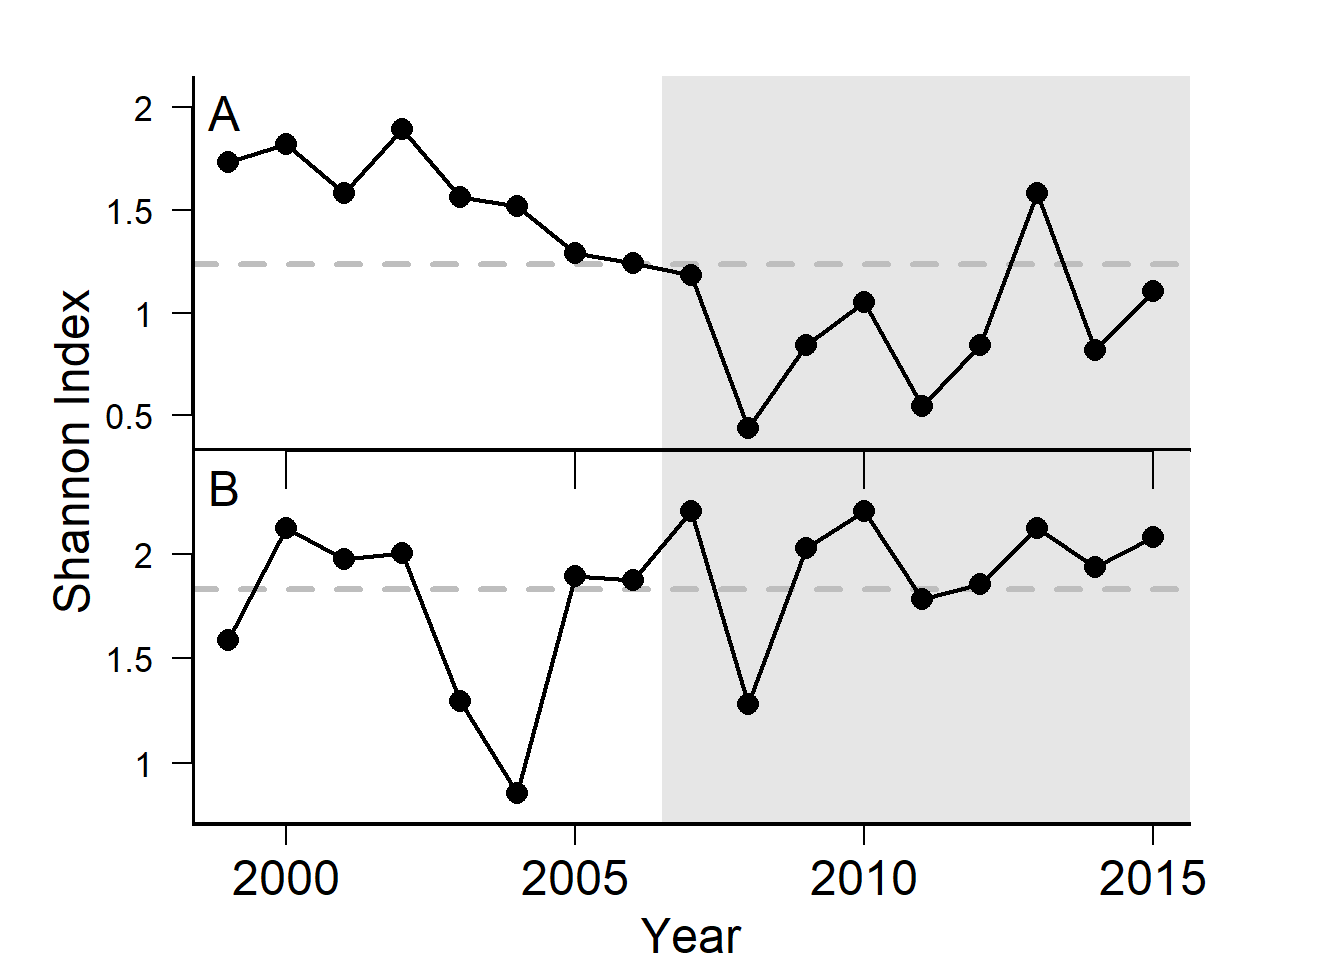
\includegraphics{C:/Users/kimberly.bastille/Desktop/tech-doc/imageslarval-diversity-1.pdf}
\caption{\label{fig:larval-diversity}Ichthyoplankton Shannon diversity in
the spring (A) and fall (B) in the Northeast Large Marine Ecosystem.}
\end{figure}

\hypertarget{comdat}{\chapter{Commercial Landings Data}\label{comdat}}

\textbf{Description}: Commercial landings data pull

\textbf{Found in}: State of the Ecosystem - Gulf of Maine \& Georges
Bank (2017, 2018, 2019), State of the Ecosystem - Mid-Atlantic (2017,
2018, 2019)

\textbf{Indicator category}: Database pull

\textbf{Contributor(s)}: Sean Lucey

\textbf{Data steward}: Sean Lucey,
\href{mailto:Sean.Lucey@noaa.gov}{\nolinkurl{Sean.Lucey@noaa.gov}}

\textbf{Point of contact}: Sean Lucey,
\href{mailto:Sean.Lucey@noaa.gov}{\nolinkurl{Sean.Lucey@noaa.gov}}

\textbf{Public availability statement}: Raw data are not publically
available due to confidentiality of individual fishery participants.
Derived indicator outputs are available
\href{https://comet.nefsc.noaa.gov/erddap/tabledap/group_landings_soe_v1.html}{here}.

\section{Methods}\label{methods-15}

Fisheries dependent data for the Northeast Shelf extend back several
decades. Data from the 1960s on are housed in the Commercial database
(CFDBS) of the Northeast Fisheries Science Center which contains the
commercial fisheries dealer purchase records (weigh-outs) collected by
NMFS Statistical Reporting Specialists and state agencies from Maine to
Virginia. The data format has changed slightly over the time series with
three distinct time frames as noted in Table \ref{tab:calibration}
below.

\begin{table}

\caption{\label{tab:calibration}Data formats}
\centering
\begin{tabular}[t]{l|l}
\hline
Table & Years\\
\hline
WOLANDS & 1964 - 1981\\
\hline
WODETS & 1982 - 1993\\
\hline
CFDETS\_AA & > 1994\\
\hline
\end{tabular}
\end{table}

Comlands is an R database pull that consolidates the landings records
from 1964 on and attempts to associate them with NAFO statistical areas
(Figure \ref{fig:StatAreaMap}). The script is divided into three
sections. The first pulls domestic landings data from the yearly
landings tables and merges them into a single data source. The second
section applies an algorithm to associate landings that are not
allocated to a statistical area using similar characteristics of the
trip to trips with known areas. The final section pulls foreign landings
from the NAFO website and rectifies species and gear codes so they can
be merged along with domestic landings.

\begin{figure}

{\centering 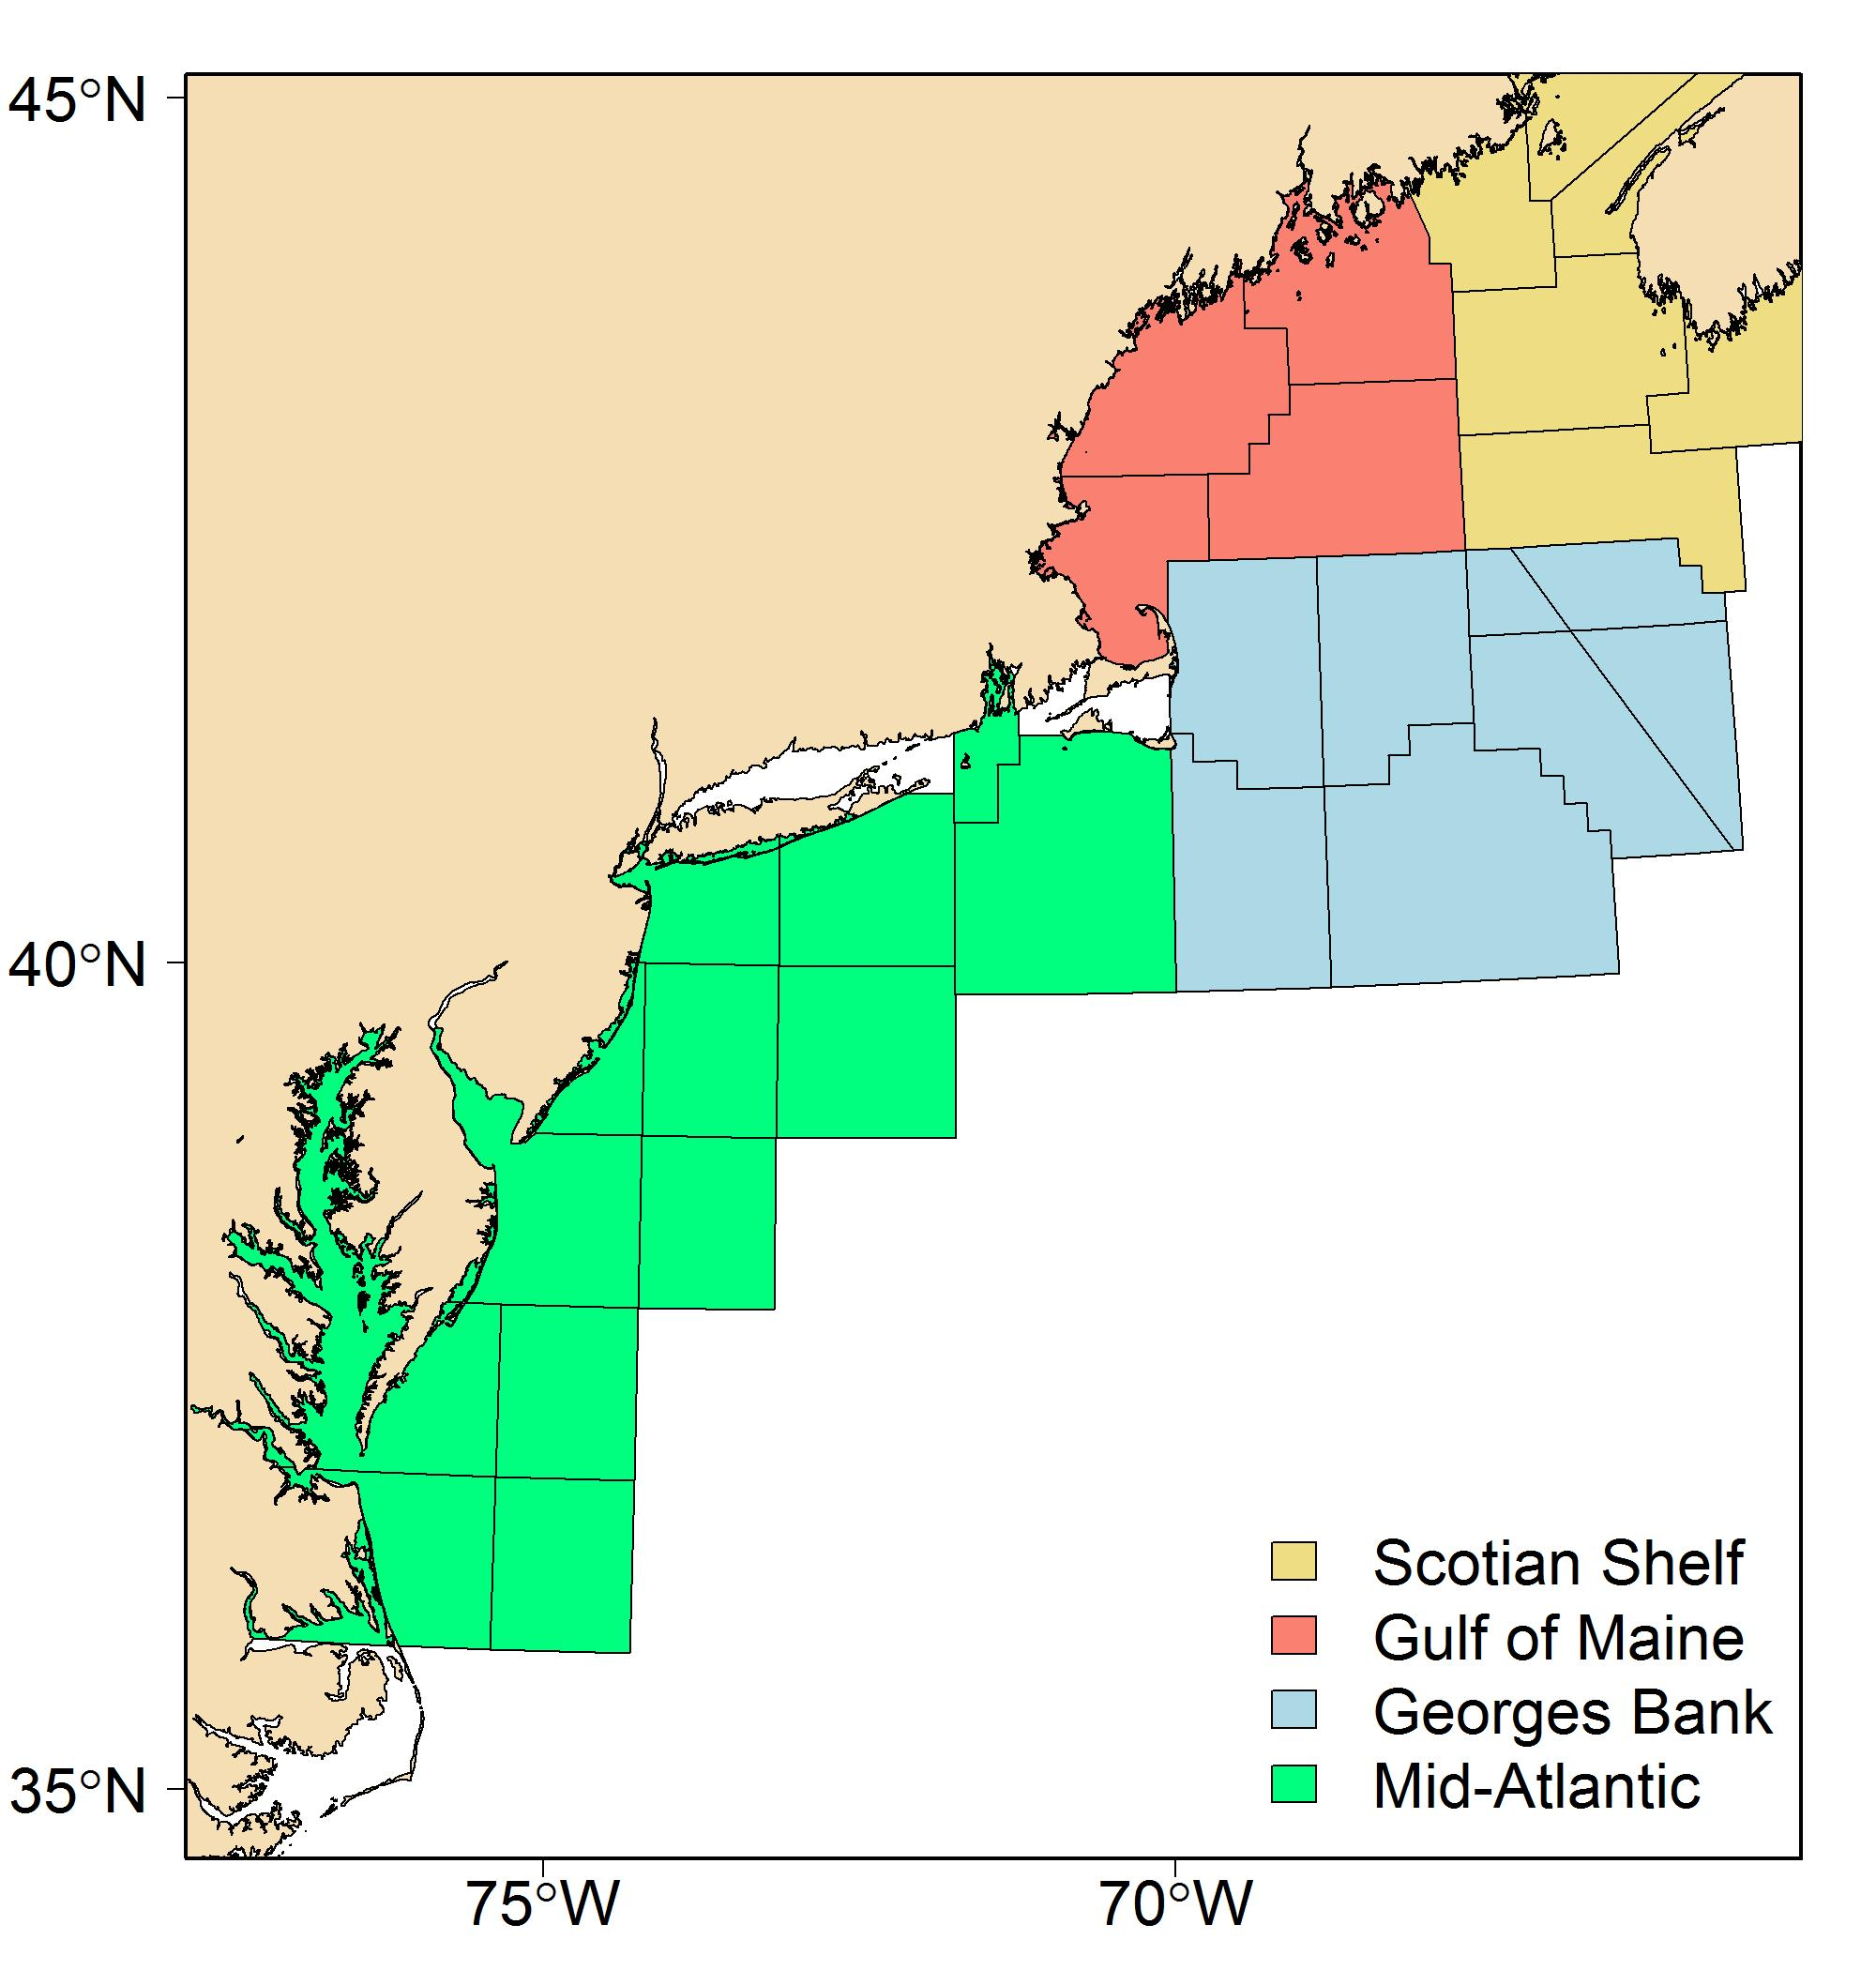
\includegraphics[width=0.5\linewidth]{C:/Users/kimberly.bastille/Desktop/tech-doc/images/Stat_Area_Map} 

}

\caption{Map of the North Atlantic Fisheries Organization (NAFO) Statistical Areas.  Colors represent the Ecological Production Unit (EPU) with which the statistical area is associated.}\label{fig:StatAreaMap}
\end{figure}

During the first section, the Comlands script pulls the temporal and
spatial information as well as vessel and gear characteristics
associated with the landings in addition to the weight, value, and
utilization code of each species in the landings record. The script
includes a toggle to use landed weights as opposed to live weights. For
all but shellfish species, live weights are used for the State of the
Ecosystem report. Due to the volume of data contained within each yearly
landings table, landings are aggregated by species, utilization code,
and area as well as by month, gear, and tonnage class. All weights are
then converted from pounds to metric tons. Landings values are also
adjusted for inflation using the Producer Price Index by Commodity for
Processed Foods and Feeds: Unprocessed and Packaged Fish. Inflation is
based on January of the terminal year of the data pull ensuring that all
values are in current dollar prices.

\begin{wraptable}{r}{0pt}
\begin{tabular}{rl}
\toprule
 & Major gear\\
\midrule
1 & Otter Trawls\\
2 & Scallop Dredges\\
3 & Other Dredges\\
4 & Gillnets\\
5 & Longlines\\
\addlinespace
6 & Seines\\
7 & Pots/Traps\\
8 & Midwater\\
9 & Other\\
\bottomrule
\end{tabular}\end{wraptable}

Several species have additional steps after the data is pulled from
CFDBS. Skates are typically landed as a species complex. In order to
segregate the catch into species, the ratio of individual skate species
in the NEFSC bottom trawl survey is used to disaggregate the landings. A
similar algorithm is used to separate silver and offshore hake which can
be mistaken for one another. Finally, Atlantic herring landings are
pulled from a separate database as the most accurate weights are housed
by the State of Maine. Comlands pulls from the State database and
replaces the less accurate numbers from the federal database.

The majority of landings data are associated with a NAFO Statistical
Area. For those that are not, Comlands attempts to assign them to an
area using similar characteristics of trips where the area is known. To
simplify this task, landings data are further aggregated into quarter
and half year, small and large vessels, and eight major gear categories
(Table \ref{tab:gears}). Landings are then proportioned to areas that
meet similar characteristics based on the proportion of landings in each
area by that temporal/vessel/gear combination. If a given attribute is
unknown, the algorithm attempts to assign it one, once again based on
matched characteristics of known trips. Statistical areas are then
assigned to their respective \protect\hyperlink{epu}{Ecological
Production Unit} (Table \ref{tab:statareas}).

\begin{table}[H]

\caption{\label{tab:statareas}Statistical areas making up each EPU}
\centering
\begin{tabular}[t]{l|l}
\hline
EPU & Stat Areas\\
\hline
Gulf of Maine & 500, 510, 512, 513, 514, 515\\
\hline
Georges Bank & 521, 522, 523, 524, 525, 526, 551, 552, 561, 562\\
\hline
Mid-Atlantic & 537, 539, 600, 612, 613, 614, 615, 616, 621, 622, 625, 626, 631, 632\\
\hline
\end{tabular}
\end{table}

The final step of Comlands is to pull the foreign landings from the
\href{https://www.nafo.int/Data/frames}{NAFO database}. US landings are
removed from this extraction so as not to be double counted. NAFO codes
and CFDBS codes differ so the script rectifies those codes to ensure
that the data is seamlessly merged into the domestic landings. Foreign
landings are flagged so that they can be removed if so desired.

\subsection{Data sources}\label{data-sources-15}

Comland is a database query of the NEFSC commercial fishery database
(CFDBS). More information about the CFDBS is available
\href{https://inport.nmfs.noaa.gov/inport/item/27401}{here}.

\subsection{Data extraction}\label{data-extraction-13}

R code used in the extraction process described above:

\begin{Shaded}
\begin{Highlighting}[]
\CommentTok{#Comland.r}
\CommentTok{#Version now controlled by git - originally part of comcatch.r}
\CommentTok{#Grab commercial landings data from US and Foreign countries (NAFO)}
\CommentTok{#Need to fix menhaden data}
\CommentTok{#SML}

\CommentTok{#Requires the following files:}
\CommentTok{# data.dir.2\textbackslash{}\textbackslash{}Comland_skates_hakes.R}
\CommentTok{# data.dir\textbackslash{}\textbackslash{}Menhaden.csv}
\CommentTok{# data.dir.3\textbackslash{}\textbackslash{}SS_NAFO_21A.csv}
\CommentTok{# data.dir.3\textbackslash{}\textbackslash{}species.txt}

\CommentTok{#User parameters}
\ControlFlowTok{if}\NormalTok{(}\KeywordTok{Sys.info}\NormalTok{()[}\StringTok{'sysname'}\NormalTok{]}\OperatorTok{==}\StringTok{"Windows"}\NormalTok{)\{}
\NormalTok{  data.dir   <-}\StringTok{ "L:}\CharTok{\textbackslash{}\textbackslash{}}\StringTok{EcoAP}\CharTok{\textbackslash{}\textbackslash{}}\StringTok{Data}\CharTok{\textbackslash{}\textbackslash{}}\StringTok{Commercial"}
\NormalTok{  data.dir.}\DecValTok{2}\NormalTok{ <-}\StringTok{ "L:}\CharTok{\textbackslash{}\textbackslash{}}\StringTok{Rworkspace}\CharTok{\textbackslash{}\textbackslash{}}\StringTok{RCom"}
\NormalTok{  data.dir.}\DecValTok{3}\NormalTok{ <-}\StringTok{ "L:}\CharTok{\textbackslash{}\textbackslash{}}\StringTok{EcoAP}\CharTok{\textbackslash{}\textbackslash{}}\StringTok{Data}\CharTok{\textbackslash{}\textbackslash{}}\StringTok{NAFO"}
\NormalTok{  out.dir    <-}\StringTok{ "L:}\CharTok{\textbackslash{}\textbackslash{}}\StringTok{EcoAP}\CharTok{\textbackslash{}\textbackslash{}}\StringTok{Data}\CharTok{\textbackslash{}\textbackslash{}}\StringTok{Commercial"}
  \KeywordTok{memory.limit}\NormalTok{(}\DecValTok{4000}\NormalTok{)}
\NormalTok{  channel <-}\StringTok{ }\KeywordTok{odbcDriverConnect}\NormalTok{()}
\NormalTok{\}}

\ControlFlowTok{if}\NormalTok{(}\KeywordTok{Sys.info}\NormalTok{()[}\StringTok{'sysname'}\NormalTok{]}\OperatorTok{==}\StringTok{"Linux"}\NormalTok{)\{}
\NormalTok{  data.dir   <-}\StringTok{ "/home/slucey/slucey/EcoAP/Data/Commercial"}
\NormalTok{  data.dir.}\DecValTok{2}\NormalTok{ <-}\StringTok{ "/home/slucey/slucey/Rworkspace/RCom"}
\NormalTok{  data.dir.}\DecValTok{3}\NormalTok{ <-}\StringTok{ "/home/slucey/slucey/EcoAP/Data/NAFO"}
\NormalTok{  out.dir    <-}\StringTok{ "/home/slucey/slucey/EcoAP/Data/Commercial"}
\NormalTok{  uid <-}\StringTok{ 'slucey'}
  \KeywordTok{cat}\NormalTok{(}\StringTok{"Oracle Password: "}\NormalTok{)}
\NormalTok{  pwd <-}\StringTok{ }\KeywordTok{scan}\NormalTok{(}\KeywordTok{stdin}\NormalTok{(), }\KeywordTok{character}\NormalTok{(), }\DataTypeTok{n =} \DecValTok{1}\NormalTok{)}
\NormalTok{\}}

\NormalTok{landed       <-}\StringTok{ 'y'} \CommentTok{#use landed weight for scallops and clams instead of live weight}
\NormalTok{foreign      <-}\StringTok{ 'y'} \CommentTok{#Mark foreign landings and keep seperate}
\NormalTok{adjust.ppi   <-}\StringTok{ 'y'} \CommentTok{#Adjust value for inflation}
\NormalTok{use.existing <-}\StringTok{ 'n'} \CommentTok{#use raw data from a previous run - saves time}
\NormalTok{sum.by       <-}\StringTok{ 'EPU'} \CommentTok{#Variable to sum landings by [EPU, stat.area]}

\CommentTok{#Final year of query}
\NormalTok{endyear <-}\StringTok{ }\DecValTok{2016}
\CommentTok{#If adjusting for inflation}
\NormalTok{refyear  <-}\StringTok{ }\DecValTok{2016}
\NormalTok{refmonth <-}\StringTok{ }\DecValTok{1}

\CommentTok{#-------------------------------------------------------------------------------}
\CommentTok{#Required packages}
\KeywordTok{library}\NormalTok{(RODBC); }\KeywordTok{library}\NormalTok{(data.table); }\KeywordTok{library}\NormalTok{(rgdal)}

\CommentTok{#-------------------------------------------------------------------------------}
\CommentTok{#User created functions }
\CommentTok{#Convert NA's to zeros}
\NormalTok{na.zero <-}\StringTok{ }\ControlFlowTok{function}\NormalTok{(x)\{}
  \ControlFlowTok{for}\NormalTok{(i }\ControlFlowTok{in} \DecValTok{1}\OperatorTok{:}\KeywordTok{length}\NormalTok{(x[}\DecValTok{1}\NormalTok{, ]))\{}
    \ControlFlowTok{if}\NormalTok{(}\KeywordTok{length}\NormalTok{(}\KeywordTok{which}\NormalTok{(}\KeywordTok{is.na}\NormalTok{(x[, i]))) }\OperatorTok{>}\StringTok{ }\DecValTok{0}\NormalTok{)\{}
\NormalTok{      x[}\KeywordTok{which}\NormalTok{(}\KeywordTok{is.na}\NormalTok{(x[, i])), i] <-}\StringTok{ }\DecValTok{0}\NormalTok{\}}
\NormalTok{    \}}
    \KeywordTok{return}\NormalTok{(x)}
\NormalTok{  \} }
  
\CommentTok{#-------------------------------------------------------------------------------}
\CommentTok{#Connect to database}
\ControlFlowTok{if}\NormalTok{(}\KeywordTok{Sys.info}\NormalTok{()[}\StringTok{'sysname'}\NormalTok{] }\OperatorTok{==}\StringTok{ "Windows"}\NormalTok{)channel <-}\StringTok{ }\KeywordTok{odbcDriverConnect}\NormalTok{()}
\ControlFlowTok{if}\NormalTok{(}\KeywordTok{Sys.info}\NormalTok{()[}\StringTok{'sysname'}\NormalTok{] }\OperatorTok{==}\StringTok{ "Linux"}\NormalTok{)  channel <-}\StringTok{ }\KeywordTok{odbcConnect}\NormalTok{(}\StringTok{'sole'}\NormalTok{, uid, pwd)}

\ControlFlowTok{if}\NormalTok{(use.existing }\OperatorTok{==}\StringTok{ 'n'}\NormalTok{)\{}
  \CommentTok{#Landings}
\NormalTok{  tables <-}\StringTok{ }\KeywordTok{c}\NormalTok{(}\KeywordTok{paste0}\NormalTok{(}\StringTok{'WOLANDS'}\NormalTok{, }\DecValTok{64}\OperatorTok{:}\DecValTok{81}\NormalTok{), }
              \KeywordTok{paste0}\NormalTok{(}\StringTok{'WODETS'}\NormalTok{,  }\DecValTok{82}\OperatorTok{:}\DecValTok{93}\NormalTok{), }
              \KeywordTok{paste0}\NormalTok{(}\StringTok{'CFDETS'}\NormalTok{,  }\DecValTok{1994}\OperatorTok{:}\NormalTok{endyear, }\StringTok{'AA'}\NormalTok{))}
  
  \CommentTok{#Generate one table}
\NormalTok{  comland <-}\StringTok{ }\KeywordTok{c}\NormalTok{()}
  \ControlFlowTok{for}\NormalTok{(i }\ControlFlowTok{in} \DecValTok{1}\OperatorTok{:}\KeywordTok{length}\NormalTok{(tables))\{}
\NormalTok{    landings.qry <-}\StringTok{ }\KeywordTok{paste}\NormalTok{(}\StringTok{"select year, month, negear, toncl1, nespp3, nespp4, area, }
\StringTok{                           spplivlb, spplndlb, sppvalue, utilcd}
\StringTok{                           from"}\NormalTok{, tables[i])}
    
\NormalTok{    comland.yr <-}\StringTok{ }\KeywordTok{as.data.table}\NormalTok{(}\KeywordTok{sqlQuery}\NormalTok{(channel, landings.qry))}
    
    \KeywordTok{setkey}\NormalTok{(comland.yr,}
\NormalTok{           YEAR,}
\NormalTok{           MONTH,}
\NormalTok{           NEGEAR,}
\NormalTok{           TONCL1,}
\NormalTok{           NESPP3,}
\NormalTok{           NESPP4,}
\NormalTok{           AREA,}
\NormalTok{           UTILCD)}
  
    \ControlFlowTok{if}\NormalTok{(landed }\OperatorTok{==}\StringTok{ 'y'}\NormalTok{) comland.yr[NESPP3 }\OperatorTok\StringTok{ }\DecValTok{743}\OperatorTok{:}\DecValTok{800}\NormalTok{, SPPLIVLB }\OperatorTok{:}\ErrorTok{=}\StringTok{ }\NormalTok{SPPLNDLB]}
    
    \CommentTok{#Sum landings and value}
    \CommentTok{#landings}
\NormalTok{    comland.yr[, V1 }\OperatorTok{:}\ErrorTok{=}\StringTok{ }\KeywordTok{sum}\NormalTok{(SPPLIVLB), by =}\StringTok{ }\KeywordTok{key}\NormalTok{(comland.yr)]}
    \CommentTok{#value}
    \CommentTok{#Fix null values}
\NormalTok{    comland.yr[}\KeywordTok{is.na}\NormalTok{(SPPVALUE), SPPVALUE }\OperatorTok{:}\ErrorTok{=}\StringTok{ }\DecValTok{0}\NormalTok{]}
\NormalTok{    comland.yr[, V2 }\OperatorTok{:}\ErrorTok{=}\StringTok{ }\KeywordTok{sum}\NormalTok{(SPPVALUE), by =}\StringTok{ }\KeywordTok{key}\NormalTok{(comland.yr)]}
    
    \CommentTok{#Remove extra rows/columns}
\NormalTok{    comland.yr <-}\StringTok{ }\KeywordTok{unique}\NormalTok{(comland.yr, }\DataTypeTok{by =} \KeywordTok{key}\NormalTok{(comland.yr))}
\NormalTok{    comland.yr[, }\KeywordTok{c}\NormalTok{(}\StringTok{'SPPLIVLB'}\NormalTok{, }\StringTok{'SPPLNDLB'}\NormalTok{, }\StringTok{'SPPVALUE'}\NormalTok{) }\OperatorTok{:}\ErrorTok{=}\StringTok{ }\OtherTok{NULL}\NormalTok{]}
    
    \CommentTok{#Rename summed columns}
    \KeywordTok{setnames}\NormalTok{(comland.yr, }\KeywordTok{c}\NormalTok{(}\StringTok{'V1'}\NormalTok{, }\StringTok{'V2'}\NormalTok{), }\KeywordTok{c}\NormalTok{(}\StringTok{'SPPLIVLB'}\NormalTok{, }\StringTok{'SPPVALUE'}\NormalTok{))}
    
\NormalTok{    comland <-}\StringTok{ }\KeywordTok{rbindlist}\NormalTok{(}\KeywordTok{list}\NormalTok{(comland, comland.yr))}
\NormalTok{  \}}
  
  \ControlFlowTok{if}\NormalTok{(landed }\OperatorTok{==}\StringTok{ 'n'}\NormalTok{) }\KeywordTok{save}\NormalTok{(comland, }\DataTypeTok{file =} \KeywordTok{file.path}\NormalTok{(out.dir, }\StringTok{"comland_raw_US.RData"}\NormalTok{))}
  \CommentTok{#Last run 8/31/16}
  \ControlFlowTok{if}\NormalTok{(landed }\OperatorTok{==}\StringTok{ 'y'}\NormalTok{) }\KeywordTok{save}\NormalTok{(comland, }\DataTypeTok{file =} \KeywordTok{file.path}\NormalTok{(out.dir, }\StringTok{"comland_raw_US_meatwt.RData"}\NormalTok{))}
  \CommentTok{#Last run 1/25/18 }
\NormalTok{\}}
\ControlFlowTok{if}\NormalTok{(use.existing }\OperatorTok{==}\StringTok{ 'y'}\NormalTok{)\{}
  \ControlFlowTok{if}\NormalTok{(landed }\OperatorTok{==}\StringTok{ 'n'}\NormalTok{) }\KeywordTok{load}\NormalTok{(}\DataTypeTok{file =} \KeywordTok{file.path}\NormalTok{(out.dir, }\StringTok{"comland_raw_US.RData"}\NormalTok{))}
  \ControlFlowTok{if}\NormalTok{(landed }\OperatorTok{==}\StringTok{ 'y'}\NormalTok{) }\KeywordTok{load}\NormalTok{(}\DataTypeTok{file =} \KeywordTok{file.path}\NormalTok{(out.dir, }\StringTok{"comland_raw_US_meatwt.RData"}\NormalTok{))  }
\NormalTok{\}}

\CommentTok{#-------------------------------------------------------------------------------}
\CommentTok{#Convert from lbs to metric tons}
\NormalTok{comland[, SPPLIVMT }\OperatorTok{:}\ErrorTok{=}\StringTok{ }\NormalTok{SPPLIVLB }\OperatorTok{*}\StringTok{ }\FloatTok{0.00045359237}\NormalTok{]}
\NormalTok{comland[, SPPLIVLB }\OperatorTok{:}\ErrorTok{=}\StringTok{ }\OtherTok{NULL}\NormalTok{]}

\CommentTok{#fix years}
\NormalTok{comland[YEAR }\OperatorTok{<}\StringTok{ }\DecValTok{100}\NormalTok{, YEAR }\OperatorTok{:}\ErrorTok{=}\StringTok{ }\NormalTok{YEAR }\OperatorTok{+}\StringTok{ }\NormalTok{1900L]}

\ControlFlowTok{if}\NormalTok{(adjust.ppi }\OperatorTok{==}\StringTok{ 'y'}\NormalTok{)\{}
    \CommentTok{#Adjust SPPVALUE for inflation}
\NormalTok{    temp <-}\StringTok{ }\KeywordTok{tempfile}\NormalTok{()}
    \KeywordTok{download.file}\NormalTok{(}\StringTok{"http://download.bls.gov/pub/time.series/wp/wp.data.3.ProcessedFoods"}\NormalTok{, temp)}
\NormalTok{    inflate <-}\StringTok{ }\KeywordTok{as.data.table}\NormalTok{(}\KeywordTok{read.delim}\NormalTok{(temp))}
    \KeywordTok{unlink}\NormalTok{(temp)}
    
\NormalTok{    inflate[, series_id }\OperatorTok{:}\ErrorTok{=}\StringTok{ }\KeywordTok{gsub}\NormalTok{(}\StringTok{" "}\NormalTok{, }\StringTok{""}\NormalTok{, inflate[, series_id])]}
\NormalTok{    deflate <-}\StringTok{ }\NormalTok{inflate[series_id }\OperatorTok{==}\StringTok{ "WPU0223"}\NormalTok{, ]}
\NormalTok{    deflate[, MONTH }\OperatorTok{:}\ErrorTok{=}\StringTok{ }\KeywordTok{as.numeric}\NormalTok{(}\KeywordTok{substr}\NormalTok{(period, }\DecValTok{2}\NormalTok{, }\DecValTok{3}\NormalTok{))]}
    \KeywordTok{setnames}\NormalTok{(deflate, }\KeywordTok{c}\NormalTok{(}\StringTok{'year'}\NormalTok{, }\StringTok{'value'}\NormalTok{), }\KeywordTok{c}\NormalTok{(}\StringTok{'YEAR'}\NormalTok{, }\StringTok{'PPI'}\NormalTok{))}
\NormalTok{    deflate <-}\StringTok{ }\NormalTok{deflate[, }\KeywordTok{list}\NormalTok{(YEAR, MONTH, PPI)]}
    
    \CommentTok{#Set yearly deflator to 0 instead of 13 to match unknown month designation}
\NormalTok{    deflate[MONTH }\OperatorTok{==}\StringTok{ }\DecValTok{13}\NormalTok{, MONTH }\OperatorTok{:}\ErrorTok{=}\StringTok{ }\DecValTok{0}\NormalTok{]}
\NormalTok{    deflate.base <-}\StringTok{ }\NormalTok{deflate[YEAR }\OperatorTok{==}\StringTok{ }\NormalTok{refyear }\OperatorTok{&}\StringTok{ }\NormalTok{MONTH }\OperatorTok{==}\StringTok{ }\NormalTok{refmonth, PPI]}
    
\NormalTok{    comland <-}\StringTok{ }\KeywordTok{merge}\NormalTok{(comland, deflate, }\DataTypeTok{by =} \KeywordTok{c}\NormalTok{(}\StringTok{'YEAR'}\NormalTok{, }\StringTok{'MONTH'}\NormalTok{), }\DataTypeTok{all.x =}\NormalTok{ T)}
\NormalTok{    comland[, SPPVALUE }\OperatorTok{:}\ErrorTok{=}\StringTok{ }\KeywordTok{round}\NormalTok{((SPPVALUE }\OperatorTok{*}\StringTok{ }\NormalTok{deflate.base) }\OperatorTok{/}\StringTok{ }\NormalTok{PPI)]}
    
    \CommentTok{#Remove extra column}
\NormalTok{    comland[, PPI }\OperatorTok{:}\ErrorTok{=}\StringTok{ }\OtherTok{NULL}\NormalTok{]}
\NormalTok{\}}
\CommentTok{#Remove market categories of parts}
\NormalTok{comland <-}\StringTok{ }\NormalTok{comland[}\OperatorTok{!}\NormalTok{NESPP4 }\OperatorTok\StringTok{ }\KeywordTok{c}\NormalTok{(}\DecValTok{119}\NormalTok{, }\DecValTok{123}\NormalTok{, }\DecValTok{125}\NormalTok{, }\DecValTok{127}\NormalTok{, }\DecValTok{812}\NormalTok{, }\DecValTok{819}\NormalTok{, }\DecValTok{828}\NormalTok{, }\DecValTok{829}\NormalTok{, }\DecValTok{1731}\NormalTok{, }\DecValTok{2351}\NormalTok{,}
                                  \DecValTok{2690}\NormalTok{, }\DecValTok{2699}\NormalTok{, }\DecValTok{3472}\NormalTok{, }\KeywordTok{as.numeric}\NormalTok{(}\KeywordTok{paste}\NormalTok{(}\DecValTok{348}\OperatorTok{:}\DecValTok{359}\NormalTok{, }\DecValTok{8}\NormalTok{, }\DataTypeTok{sep =} \StringTok{''}\NormalTok{)), }
                                  \DecValTok{3868}\NormalTok{, }\KeywordTok{as.numeric}\NormalTok{(}\KeywordTok{paste}\NormalTok{(}\DecValTok{469}\OperatorTok{:}\DecValTok{471}\NormalTok{, }\DecValTok{4}\NormalTok{, }\DataTypeTok{sep =} \StringTok{''}\NormalTok{)), }
                                  \KeywordTok{as.numeric}\NormalTok{(}\KeywordTok{paste}\NormalTok{(}\DecValTok{480}\OperatorTok{:}\DecValTok{499}\NormalTok{, }\DecValTok{8}\NormalTok{, }\DataTypeTok{sep =}\StringTok{''}\NormalTok{)), }\DecValTok{5018}\NormalTok{, }\DecValTok{5039}\NormalTok{, }
                                  \DecValTok{5261}\NormalTok{, }\DecValTok{5265}\NormalTok{), ]}

\CommentTok{#Generate NESPP3 and MKTCAT in comland data}
\NormalTok{comland[NESPP4 }\OperatorTok{<}\StringTok{ }\DecValTok{100}\NormalTok{,                MKTCAT }\OperatorTok{:}\ErrorTok{=}\StringTok{ }\KeywordTok{as.numeric}\NormalTok{(}\KeywordTok{substring}\NormalTok{(NESPP4, }\DecValTok{2}\NormalTok{, }\DecValTok{2}\NormalTok{))]}
\NormalTok{comland[NESPP4 }\OperatorTok{>}\StringTok{ }\DecValTok{99} \OperatorTok{&}\StringTok{ }\NormalTok{NESPP4 }\OperatorTok{<}\StringTok{ }\DecValTok{1000}\NormalTok{, MKTCAT }\OperatorTok{:}\ErrorTok{=}\StringTok{ }\KeywordTok{as.numeric}\NormalTok{(}\KeywordTok{substring}\NormalTok{(NESPP4, }\DecValTok{3}\NormalTok{, }\DecValTok{3}\NormalTok{))]}
\NormalTok{comland[NESPP4 }\OperatorTok{>}\StringTok{ }\DecValTok{999}\NormalTok{,                MKTCAT }\OperatorTok{:}\ErrorTok{=}\StringTok{ }\KeywordTok{as.numeric}\NormalTok{(}\KeywordTok{substring}\NormalTok{(NESPP4, }\DecValTok{4}\NormalTok{, }\DecValTok{4}\NormalTok{))]}

\CommentTok{#drop NESPP4}
\NormalTok{comland[, NESPP4 }\OperatorTok{:}\ErrorTok{=}\StringTok{ }\OtherTok{NULL}\NormalTok{]}

\CommentTok{#Deal with Hakes and Skates------------------------------------------------------------------}
\KeywordTok{source}\NormalTok{(}\KeywordTok{file.path}\NormalTok{(data.dir.}\DecValTok{2}\NormalTok{, }\StringTok{'Comland_skates_hakes.R'}\NormalTok{))}

\CommentTok{#get little skates and winter skates from skates(ns) - use survey in half years}
\CommentTok{#Generate Half year variable in comland}
\NormalTok{comland.skates <-}\StringTok{ }\NormalTok{comland[NESPP3 }\OperatorTok{==}\StringTok{ }\DecValTok{365}\NormalTok{, ]}
\NormalTok{comland.skates[MONTH }\OperatorTok\StringTok{ }\DecValTok{1}\OperatorTok{:}\DecValTok{6}\NormalTok{,  Half }\OperatorTok{:}\ErrorTok{=}\StringTok{ }\DecValTok{1}\NormalTok{]}
\NormalTok{comland.skates[MONTH }\OperatorTok\StringTok{ }\DecValTok{7}\OperatorTok{:}\DecValTok{12}\NormalTok{, Half }\OperatorTok{:}\ErrorTok{=}\StringTok{ }\DecValTok{2}\NormalTok{]}

\KeywordTok{setkey}\NormalTok{(skate.hake.us,}
\NormalTok{       YEAR,}
\NormalTok{       Half,}
\NormalTok{       AREA)}

\NormalTok{comland.skates <-}\StringTok{ }\KeywordTok{merge}\NormalTok{(comland.skates, skate.hake.us, }\DataTypeTok{by =} \KeywordTok{key}\NormalTok{(skate.hake.us), }\DataTypeTok{all.x =}\NormalTok{ T)}

\NormalTok{comland.skates[, little       }\OperatorTok{:}\ErrorTok{=}\StringTok{ }\NormalTok{little.per }\OperatorTok{*}\StringTok{ }\NormalTok{SPPLIVMT]}
\NormalTok{comland.skates[, little.value }\OperatorTok{:}\ErrorTok{=}\StringTok{ }\KeywordTok{round}\NormalTok{(little.per }\OperatorTok{*}\StringTok{ }\NormalTok{SPPVALUE)]}
\NormalTok{comland.skates[}\KeywordTok{is.na}\NormalTok{(little),       little       }\OperatorTok{:}\ErrorTok{=}\StringTok{ }\DecValTok{0}\NormalTok{]}
\NormalTok{comland.skates[}\KeywordTok{is.na}\NormalTok{(little.value), little.value }\OperatorTok{:}\ErrorTok{=}\StringTok{ }\DecValTok{0}\NormalTok{]}

\NormalTok{comland.skates[, winter       }\OperatorTok{:}\ErrorTok{=}\StringTok{ }\NormalTok{winter.per }\OperatorTok{*}\StringTok{ }\NormalTok{SPPLIVMT]}
\NormalTok{comland.skates[, winter.value }\OperatorTok{:}\ErrorTok{=}\StringTok{ }\KeywordTok{round}\NormalTok{(winter.per }\OperatorTok{*}\StringTok{ }\NormalTok{SPPVALUE)]}
\NormalTok{comland.skates[}\KeywordTok{is.na}\NormalTok{(winter),       winter       }\OperatorTok{:}\ErrorTok{=}\StringTok{ }\DecValTok{0}\NormalTok{]}
\NormalTok{comland.skates[}\KeywordTok{is.na}\NormalTok{(winter.value), winter.value }\OperatorTok{:}\ErrorTok{=}\StringTok{ }\DecValTok{0}\NormalTok{]}

\NormalTok{comland.skates[, other.skate       }\OperatorTok{:}\ErrorTok{=}\StringTok{ }\NormalTok{SPPLIVMT }\OperatorTok{-}\StringTok{ }\NormalTok{(little       }\OperatorTok{+}\StringTok{ }\NormalTok{winter)]}
\NormalTok{comland.skates[, other.skate.value }\OperatorTok{:}\ErrorTok{=}\StringTok{ }\NormalTok{SPPVALUE }\OperatorTok{-}\StringTok{ }\NormalTok{(little.value }\OperatorTok{+}\StringTok{ }\NormalTok{winter.value)]}

\CommentTok{#Little (366), winter (367), skates(ns) (365)}
\CommentTok{#put skates in comland format to merge back}
\NormalTok{little <-}\StringTok{ }\NormalTok{comland.skates[, }\KeywordTok{list}\NormalTok{(YEAR, Half, AREA, MONTH, NEGEAR,}
\NormalTok{                                TONCL1, NESPP3, UTILCD, MKTCAT, little, }
\NormalTok{                                little.value)]}
\NormalTok{little[, NESPP3 }\OperatorTok{:}\ErrorTok{=}\StringTok{ }\DecValTok{366}\NormalTok{]}
\KeywordTok{setnames}\NormalTok{(little, }\KeywordTok{c}\NormalTok{(}\StringTok{'little'}\NormalTok{, }\StringTok{'little.value'}\NormalTok{), }\KeywordTok{c}\NormalTok{(}\StringTok{'SPPLIVMT'}\NormalTok{, }\StringTok{'SPPVALUE'}\NormalTok{))}
\NormalTok{little <-}\StringTok{ }\NormalTok{little[SPPLIVMT }\OperatorTok{>}\StringTok{ }\DecValTok{0}\NormalTok{, ]}

\NormalTok{winter <-}\StringTok{ }\NormalTok{comland.skates[, }\KeywordTok{list}\NormalTok{(YEAR, Half, AREA, MONTH, NEGEAR,}
\NormalTok{                                TONCL1, NESPP3, UTILCD, MKTCAT, winter, }
\NormalTok{                                winter.value)]}
\NormalTok{winter[, NESPP3 }\OperatorTok{:}\ErrorTok{=}\StringTok{ }\DecValTok{367}\NormalTok{]}
\KeywordTok{setnames}\NormalTok{(winter, }\KeywordTok{c}\NormalTok{(}\StringTok{'winter'}\NormalTok{, }\StringTok{'winter.value'}\NormalTok{), }\KeywordTok{c}\NormalTok{(}\StringTok{'SPPLIVMT'}\NormalTok{, }\StringTok{'SPPVALUE'}\NormalTok{))}
\NormalTok{winter <-}\StringTok{ }\NormalTok{winter[SPPLIVMT }\OperatorTok{>}\StringTok{ }\DecValTok{0}\NormalTok{, ]}

\NormalTok{other <-}\StringTok{ }\NormalTok{comland.skates[, }\KeywordTok{list}\NormalTok{(YEAR, Half, AREA, MONTH, NEGEAR,}
\NormalTok{                               TONCL1, NESPP3, UTILCD, MKTCAT, other.skate, }
\NormalTok{                               other.skate.value)]}
\NormalTok{other[, NESPP3 }\OperatorTok{:}\ErrorTok{=}\StringTok{ }\DecValTok{365}\NormalTok{]}
\KeywordTok{setnames}\NormalTok{(other, }\KeywordTok{c}\NormalTok{(}\StringTok{'other.skate'}\NormalTok{, }\StringTok{'other.skate.value'}\NormalTok{), }\KeywordTok{c}\NormalTok{(}\StringTok{'SPPLIVMT'}\NormalTok{, }\StringTok{'SPPVALUE'}\NormalTok{))}
\NormalTok{other <-}\StringTok{ }\NormalTok{other[SPPLIVMT }\OperatorTok{>}\StringTok{ }\DecValTok{0}\NormalTok{, ]}

\CommentTok{#merge all three and reformat for comland}
\NormalTok{skates.add.back <-}\StringTok{ }\KeywordTok{rbindlist}\NormalTok{(}\KeywordTok{list}\NormalTok{(little, winter, other))}

\NormalTok{skates.add.back[, Half }\OperatorTok{:}\ErrorTok{=}\StringTok{ }\OtherTok{NULL}\NormalTok{]}
\KeywordTok{setcolorder}\NormalTok{(skates.add.back, }\KeywordTok{names}\NormalTok{(comland))}

\NormalTok{comland <-}\StringTok{ }\KeywordTok{rbindlist}\NormalTok{(}\KeywordTok{list}\NormalTok{(comland[NESPP3 }\OperatorTok{!=}\StringTok{ }\DecValTok{365}\NormalTok{, ], skates.add.back))  }

\CommentTok{#get silver hake from mixed hakes - use survey in half years}
\CommentTok{#Generate Half year variable in comland}
\NormalTok{comland.hakes <-}\StringTok{ }\NormalTok{comland[NESPP3 }\OperatorTok{==}\StringTok{ }\DecValTok{507}\NormalTok{, ]}
\NormalTok{comland.hakes[MONTH }\OperatorTok\StringTok{ }\DecValTok{1}\OperatorTok{:}\DecValTok{6}\NormalTok{,  Half }\OperatorTok{:}\ErrorTok{=}\StringTok{ }\DecValTok{1}\NormalTok{]}
\NormalTok{comland.hakes[MONTH }\OperatorTok\StringTok{ }\DecValTok{7}\OperatorTok{:}\DecValTok{12}\NormalTok{, Half }\OperatorTok{:}\ErrorTok{=}\StringTok{ }\DecValTok{2}\NormalTok{]}

\NormalTok{comland.hakes <-}\StringTok{ }\KeywordTok{merge}\NormalTok{(comland.hakes, skate.hake.us, }\DataTypeTok{by =} \KeywordTok{key}\NormalTok{(skate.hake.us), }\DataTypeTok{all.x =}\NormalTok{ T)}

\NormalTok{comland.hakes[, silver       }\OperatorTok{:}\ErrorTok{=}\StringTok{ }\NormalTok{silver.per }\OperatorTok{*}\StringTok{ }\NormalTok{SPPLIVMT]}
\NormalTok{comland.hakes[, silver.value }\OperatorTok{:}\ErrorTok{=}\StringTok{ }\KeywordTok{round}\NormalTok{(silver.per }\OperatorTok{*}\StringTok{ }\NormalTok{SPPVALUE)]}
\NormalTok{comland.hakes[}\KeywordTok{is.na}\NormalTok{(silver),       silver       }\OperatorTok{:}\ErrorTok{=}\StringTok{ }\DecValTok{0}\NormalTok{]}
\NormalTok{comland.hakes[}\KeywordTok{is.na}\NormalTok{(silver.value), silver.value }\OperatorTok{:}\ErrorTok{=}\StringTok{ }\DecValTok{0}\NormalTok{]}

\NormalTok{comland.hakes[, off.hake       }\OperatorTok{:}\ErrorTok{=}\StringTok{ }\NormalTok{SPPLIVMT }\OperatorTok{-}\StringTok{ }\NormalTok{silver]}
\NormalTok{comland.hakes[, off.hake.value }\OperatorTok{:}\ErrorTok{=}\StringTok{ }\NormalTok{SPPVALUE }\OperatorTok{-}\StringTok{ }\NormalTok{silver.value]}

\CommentTok{#Silver hake (509), mix hakes (507)}
\CommentTok{#put hakes in comland format to merge back}
\NormalTok{silver <-}\StringTok{ }\NormalTok{comland.hakes[, }\KeywordTok{list}\NormalTok{(YEAR, Half, AREA, MONTH, NEGEAR,}
\NormalTok{                               TONCL1, NESPP3, UTILCD, MKTCAT, silver, }
\NormalTok{                               silver.value)]}
\NormalTok{silver[, NESPP3 }\OperatorTok{:}\ErrorTok{=}\StringTok{ }\DecValTok{509}\NormalTok{]}
\KeywordTok{setnames}\NormalTok{(silver, }\KeywordTok{c}\NormalTok{(}\StringTok{'silver'}\NormalTok{, }\StringTok{'silver.value'}\NormalTok{), }\KeywordTok{c}\NormalTok{(}\StringTok{'SPPLIVMT'}\NormalTok{, }\StringTok{'SPPVALUE'}\NormalTok{))}
\NormalTok{silver <-}\StringTok{ }\NormalTok{silver[SPPLIVMT }\OperatorTok{>}\StringTok{ }\DecValTok{0}\NormalTok{, ]}

\NormalTok{offshore <-}\StringTok{ }\NormalTok{comland.hakes[, }\KeywordTok{list}\NormalTok{(YEAR, Half, AREA, MONTH, NEGEAR,}
\NormalTok{                                 TONCL1, NESPP3, UTILCD, MKTCAT, off.hake, }
\NormalTok{                                 off.hake.value)]}
\NormalTok{offshore[, NESPP3 }\OperatorTok{:}\ErrorTok{=}\StringTok{ }\DecValTok{507}\NormalTok{]}
\KeywordTok{setnames}\NormalTok{(offshore, }\KeywordTok{c}\NormalTok{(}\StringTok{'off.hake'}\NormalTok{, }\StringTok{'off.hake.value'}\NormalTok{), }\KeywordTok{c}\NormalTok{(}\StringTok{'SPPLIVMT'}\NormalTok{, }\StringTok{'SPPVALUE'}\NormalTok{))}
\NormalTok{offshore <-}\StringTok{ }\NormalTok{offshore[SPPLIVMT }\OperatorTok{>}\StringTok{ }\DecValTok{0}\NormalTok{, ]}

\CommentTok{#merge both and reformat for comland}
\NormalTok{hakes.add.back <-}\StringTok{ }\KeywordTok{rbindlist}\NormalTok{(}\KeywordTok{list}\NormalTok{(silver, offshore))}

\NormalTok{hakes.add.back[, Half }\OperatorTok{:}\ErrorTok{=}\StringTok{ }\OtherTok{NULL}\NormalTok{]}
\KeywordTok{setcolorder}\NormalTok{(hakes.add.back, }\KeywordTok{names}\NormalTok{(comland))}

\NormalTok{comland <-}\StringTok{ }\KeywordTok{rbindlist}\NormalTok{(}\KeywordTok{list}\NormalTok{(comland[NESPP3 }\OperatorTok{!=}\StringTok{ }\DecValTok{507}\NormalTok{, ], hakes.add.back))}


\CommentTok{#Herring---------------------------------------------------------------------------------}
\CommentTok{#Herring data is housed by the state of Maine.}
\NormalTok{herr.qry <-}\StringTok{ "select year, month, stock_area, negear, gearname, keptmt, discmt}
\StringTok{             from maine_herring_catch"}

\NormalTok{herr.catch <-}\StringTok{ }\KeywordTok{as.data.table}\NormalTok{(}\KeywordTok{sqlQuery}\NormalTok{(channel, herr.qry))}
\KeywordTok{setkey}\NormalTok{(herr.catch, YEAR, MONTH, STOCK_AREA, NEGEAR)}

\NormalTok{herring <-}\StringTok{ }\NormalTok{herr.catch[, }\KeywordTok{list}\NormalTok{(}\KeywordTok{sum}\NormalTok{(KEPTMT), }\KeywordTok{sum}\NormalTok{(DISCMT)), by =}\StringTok{ }\KeywordTok{key}\NormalTok{(herr.catch)]}
\KeywordTok{setnames}\NormalTok{(herring, }\KeywordTok{c}\NormalTok{(}\StringTok{'STOCK_AREA'}\NormalTok{, }\StringTok{'V1'}\NormalTok{, }\StringTok{'V2'}\NormalTok{),}
                  \KeywordTok{c}\NormalTok{(}\StringTok{'AREA'}\NormalTok{, }\StringTok{'SPPLIVMT'}\NormalTok{, }\StringTok{'DISCMT'}\NormalTok{))}

\CommentTok{#Using averages from comland to fill in categories}
\NormalTok{herring[, MKTCAT }\OperatorTok{:}\ErrorTok{=}\StringTok{ }\DecValTok{5}\NormalTok{]}
\NormalTok{herring[, TONCL1 }\OperatorTok{:}\ErrorTok{=}\StringTok{ }\DecValTok{2}\NormalTok{]}
\NormalTok{herring[, UTILCD }\OperatorTok{:}\ErrorTok{=}\StringTok{ }\DecValTok{0}\NormalTok{]}

\CommentTok{#compute price/utilization from CF tables}
\NormalTok{herring.comland <-}\StringTok{ }\NormalTok{comland[NESPP3 }\OperatorTok{==}\StringTok{ }\DecValTok{168}\NormalTok{, ]}
\CommentTok{#Price from comland}
\NormalTok{herring.price <-}\StringTok{ }\NormalTok{herring.comland[, (}\KeywordTok{sum}\NormalTok{(SPPVALUE) }\OperatorTok{/}\StringTok{ }\KeywordTok{sum}\NormalTok{(SPPLIVMT)), by =}\StringTok{ }\KeywordTok{c}\NormalTok{(}\StringTok{'YEAR'}\NormalTok{, }\StringTok{'MONTH'}\NormalTok{)]}
\KeywordTok{setnames}\NormalTok{(herring.price, }\StringTok{'V1'}\NormalTok{, }\StringTok{'price'}\NormalTok{)}
\NormalTok{herring <-}\StringTok{ }\KeywordTok{merge}\NormalTok{(herring, herring.price, }\DataTypeTok{by =} \KeywordTok{c}\NormalTok{(}\StringTok{'YEAR'}\NormalTok{, }\StringTok{'MONTH'}\NormalTok{), }\DataTypeTok{all.x =}\NormalTok{ T)}
\CommentTok{#Use 1964 prices for < 1964}
\NormalTok{herring[YEAR }\OperatorTok{<}\StringTok{ }\DecValTok{1964}\NormalTok{, price }\OperatorTok{:}\ErrorTok{=}\StringTok{ }\KeywordTok{mean}\NormalTok{(herring[YEAR }\OperatorTok{==}\StringTok{ }\DecValTok{1964}\NormalTok{, price])]}
\CommentTok{#Calculate SPPVALUE from price}
\NormalTok{herring[, SPPVALUE }\OperatorTok{:}\ErrorTok{=}\StringTok{ }\KeywordTok{round}\NormalTok{(price }\OperatorTok{*}\StringTok{ }\NormalTok{SPPLIVMT)]}

\CommentTok{#Utilization from comland}
\NormalTok{herring.util <-}\StringTok{ }\NormalTok{herring.comland[, }\KeywordTok{sum}\NormalTok{(SPPLIVMT), by =}\StringTok{ }\KeywordTok{c}\NormalTok{(}\StringTok{'YEAR'}\NormalTok{, }\StringTok{'MONTH'}\NormalTok{, }\StringTok{'UTILCD'}\NormalTok{)]}
\KeywordTok{setnames}\NormalTok{(herring.util, }\StringTok{'V1'}\NormalTok{, }\StringTok{'SPPLIVMT'}\NormalTok{)}
\NormalTok{herring.util[, SPPLIVMT.ALL }\OperatorTok{:}\ErrorTok{=}\StringTok{ }\KeywordTok{sum}\NormalTok{(SPPLIVMT), by =}\StringTok{ }\KeywordTok{c}\NormalTok{(}\StringTok{'YEAR'}\NormalTok{, }\StringTok{'MONTH'}\NormalTok{)]}
\NormalTok{herring.util[, Prop }\OperatorTok{:}\ErrorTok{=}\StringTok{ }\NormalTok{SPPLIVMT}\OperatorTok{/}\NormalTok{SPPLIVMT.ALL]}
\KeywordTok{setorder}\NormalTok{(herring.util, YEAR, MONTH, Prop)}
\NormalTok{herring.util[, cum.prop }\OperatorTok{:}\ErrorTok{=}\StringTok{ }\KeywordTok{cumsum}\NormalTok{(Prop), by =}\StringTok{ }\KeywordTok{c}\NormalTok{(}\StringTok{'YEAR'}\NormalTok{, }\StringTok{'MONTH'}\NormalTok{)]}

\CommentTok{#Apply proportions to Maine data set}
\CommentTok{#Not pulled all the time - current through 2017}
\NormalTok{herring[, Total }\OperatorTok{:}\ErrorTok{=}\StringTok{ }\KeywordTok{sum}\NormalTok{(SPPLIVMT), by =}\StringTok{ }\KeywordTok{c}\NormalTok{(}\StringTok{'YEAR'}\NormalTok{, }\StringTok{'MONTH'}\NormalTok{)]}
\NormalTok{herring[, Prop }\OperatorTok{:}\ErrorTok{=}\StringTok{ }\NormalTok{SPPLIVMT }\OperatorTok{/}\StringTok{ }\NormalTok{Total]}
\KeywordTok{setorder}\NormalTok{(herring, YEAR, MONTH, Prop)}
\NormalTok{herring[, cum.prop }\OperatorTok{:}\ErrorTok{=}\StringTok{ }\KeywordTok{cumsum}\NormalTok{(Prop), by =}\StringTok{ }\KeywordTok{c}\NormalTok{(}\StringTok{'YEAR'}\NormalTok{, }\StringTok{'MONTH'}\NormalTok{)]}

\ControlFlowTok{for}\NormalTok{(iyear }\ControlFlowTok{in} \KeywordTok{unique}\NormalTok{(herring.util[, YEAR]))\{}
  \ControlFlowTok{for}\NormalTok{(imonth }\ControlFlowTok{in} \KeywordTok{unique}\NormalTok{(herring.util[YEAR }\OperatorTok{==}\StringTok{ }\NormalTok{iyear, MONTH]))\{}
\NormalTok{    cum.prop.low <-}\StringTok{ }\DecValTok{0}
    \ControlFlowTok{for}\NormalTok{(iutil }\ControlFlowTok{in}\NormalTok{ herring.util[YEAR }\OperatorTok{==}\StringTok{ }\NormalTok{iyear }\OperatorTok{&}\StringTok{ }\NormalTok{MONTH }\OperatorTok{==}\StringTok{ }\NormalTok{imonth, UTILCD])\{}
\NormalTok{      cum.prop.high <-}\StringTok{ }\NormalTok{herring.util[YEAR }\OperatorTok{==}\StringTok{ }\NormalTok{iyear }\OperatorTok{&}\StringTok{ }\NormalTok{MONTH }\OperatorTok{==}\StringTok{ }\NormalTok{imonth }\OperatorTok{&}\StringTok{ }
\StringTok{                                      }\NormalTok{UTILCD }\OperatorTok{==}\StringTok{ }\NormalTok{iutil, cum.prop]}
\NormalTok{      herring[YEAR }\OperatorTok{==}\StringTok{ }\NormalTok{iyear }\OperatorTok{&}\StringTok{ }\NormalTok{MONTH }\OperatorTok{==}\StringTok{ }\NormalTok{imonth }\OperatorTok{&}\StringTok{ }\NormalTok{cum.prop }\OperatorTok{<=}\StringTok{ }\NormalTok{cum.prop.high }\OperatorTok{&}
\StringTok{                }\NormalTok{cum.prop }\OperatorTok{>}\StringTok{ }\NormalTok{cum.prop.low, UTILCD }\OperatorTok{:}\ErrorTok{=}\StringTok{ }\NormalTok{iutil]}
\NormalTok{      cum.prop.low <-}\StringTok{ }\NormalTok{cum.prop.high}
\NormalTok{    \}}
\NormalTok{  \}}
\NormalTok{\}}

\CommentTok{#fix column headings}
\NormalTok{herring[, }\KeywordTok{c}\NormalTok{(}\StringTok{'Total'}\NormalTok{, }\StringTok{'Prop'}\NormalTok{, }\StringTok{'cum.prop'}\NormalTok{, }\StringTok{'price'}\NormalTok{, }\StringTok{'DISCMT'}\NormalTok{) }\OperatorTok{:}\ErrorTok{=}\StringTok{ }\OtherTok{NULL}\NormalTok{]}
\NormalTok{herring[, NESPP3 }\OperatorTok{:}\ErrorTok{=}\StringTok{ }\DecValTok{168}\NormalTok{]}
\KeywordTok{setcolorder}\NormalTok{(herring, }\KeywordTok{names}\NormalTok{(comland))}

\CommentTok{#remove herring from data pull and add in Maine numbers}
\NormalTok{comland <-}\StringTok{ }\KeywordTok{rbindlist}\NormalTok{(}\KeywordTok{list}\NormalTok{(comland[NESPP3 }\OperatorTok{!=}\StringTok{ }\DecValTok{168}\NormalTok{, ], herring))}

\CommentTok{#Menhaden------------------------------------------------------------------------------------}
\NormalTok{##fix menhaden records - data from Tom Miller/ Andre Bouchheister}
\CommentTok{#menhaden <- as.data.table(read.csv(paste(data.dir, "Menhaden.csv", sep = '')))}
\CommentTok{#menhaden.mab <- menhaden[, MA.Total + CB.Total, by = Year]}
\NormalTok{##file metric is 1000s of lbs - convert to mt}
\CommentTok{#menhaden.mab[, SPPLIVMT := (V1 * 1000) *  0.00045359237]}
\CommentTok{#menhaden.mab[, V1 := NULL]}
\CommentTok{#}
\CommentTok{#menhaden.gom <- menhaden[, list(Year, NE.Total)]}
\CommentTok{#menhaden.gom[, SPPLIVMT := (NE.Total * 1000) *  0.00045359237]}
\CommentTok{#menhaden.gom[, NE.Total := NULL]}

\CommentTok{#save(comland, file = paste(out.dir, "Comland_unkA.RData", sep = ''))}

\CommentTok{#Deal with unknowns-------------------------------------------------------------------------}
\NormalTok{comland[NEGEAR }\OperatorTok{==}\StringTok{ }\DecValTok{999}\NormalTok{,  NEGEAR }\OperatorTok{:}\ErrorTok{=}\StringTok{ }\DecValTok{0}\NormalTok{]}
\NormalTok{comland[}\KeywordTok{is.na}\NormalTok{(TONCL1),  TONCL1 }\OperatorTok{:}\ErrorTok{=}\StringTok{ }\DecValTok{0}\NormalTok{]}
\NormalTok{comland[}\KeywordTok{is.na}\NormalTok{(AREA),    AREA   }\OperatorTok{:}\ErrorTok{=}\StringTok{ }\KeywordTok{as.factor}\NormalTok{(}\DecValTok{0}\NormalTok{)]}
\NormalTok{comland[AREA }\OperatorTok{==}\StringTok{ }\DecValTok{999}\NormalTok{,    AREA   }\OperatorTok{:}\ErrorTok{=}\StringTok{ }\KeywordTok{as.factor}\NormalTok{(}\DecValTok{0}\NormalTok{)]}
\NormalTok{comland[}\KeywordTok{is.na}\NormalTok{(MKTCAT),  MKTCAT }\OperatorTok{:}\ErrorTok{=}\StringTok{ }\DecValTok{0}\NormalTok{]}
\NormalTok{comland[}\KeywordTok{is.na}\NormalTok{(UTILCD),  UTILCD }\OperatorTok{:}\ErrorTok{=}\StringTok{ }\DecValTok{0}\NormalTok{]}

\CommentTok{#1 - drop unknown species/landings}
\NormalTok{comland <-}\StringTok{ }\NormalTok{comland[NESPP3 }\OperatorTok{!=}\StringTok{ }\DecValTok{0} \OperatorTok{&}\StringTok{ }\NormalTok{SPPLIVMT }\OperatorTok{!=}\StringTok{ }\DecValTok{0}\NormalTok{, ]}

\CommentTok{#Sumarry tables}
\CommentTok{#missing area}
\CommentTok{#known.area <-   comland[AREA != 0, sum(SPPLIVMT), by = NESPP3]}
\CommentTok{#unknown.area <- comland[AREA == 0, sum(SPPLIVMT), by = NESPP3]}
\CommentTok{#setnames(known.area,   "V1", "AREA.MT.known")}
\CommentTok{#setnames(unknown.area, "V1", "AREA.MT.unknown")}
\CommentTok{#missing.table <- merge(known.area, unknown.area, by = 'NESPP3', all = T)}
\CommentTok{#}
\CommentTok{#missing.table[is.na(AREA.MT.known),   AREA.MT.known   := 0]}
\CommentTok{#missing.table[is.na(AREA.MT.unknown), AREA.MT.unknown := 0]}
\CommentTok{#missing.table[, AREA.Ratio := AREA.MT.unknown / AREA.MT.known]}
\CommentTok{#}
\NormalTok{##missing month}
\CommentTok{#known.month <-   comland[MONTH != 0, sum(SPPLIVMT), by = NESPP3]}
\CommentTok{#unknown.month <- comland[MONTH == 0, sum(SPPLIVMT), by = NESPP3]}
\CommentTok{#setnames(known.month,   "V1", "MONTH.MT.known")}
\CommentTok{#setnames(unknown.month, "V1", "MONTH.MT.unknown")}
\CommentTok{#missing.table <- merge(missing.table, known.month,   by = 'NESPP3', all = T)}
\CommentTok{#missing.table <- merge(missing.table, unknown.month, by = 'NESPP3', all = T)}
\CommentTok{#}
\CommentTok{#missing.table[is.na(MONTH.MT.known),   MONTH.MT.known   := 0]}
\CommentTok{#missing.table[is.na(MONTH.MT.unknown), MONTH.MT.unknown := 0]}
\CommentTok{#missing.table[, MONTH.Ratio := MONTH.MT.unknown / MONTH.MT.known]}
\CommentTok{#}
\NormalTok{##missing gear}
\CommentTok{#known.gear <-   comland[NEGEAR != 0, sum(SPPLIVMT), by = NESPP3]}
\CommentTok{#unknown.gear <- comland[NEGEAR == 0, sum(SPPLIVMT), by = NESPP3]}
\CommentTok{#setnames(known.gear,   "V1", "GEAR.MT.known")}
\CommentTok{#setnames(unknown.gear, "V1", "GEAR.MT.unknown")}
\CommentTok{#missing.table <- merge(missing.table, known.gear,   by = 'NESPP3', all = T)}
\CommentTok{#missing.table <- merge(missing.table, unknown.gear, by = 'NESPP3', all = T)}
\CommentTok{#}
\CommentTok{#missing.table[is.na(GEAR.MT.known),   GEAR.MT.known   := 0]}
\CommentTok{#missing.table[is.na(GEAR.MT.unknown), GEAR.MT.unknown := 0]}
\CommentTok{#missing.table[, GEAR.Ratio := GEAR.MT.unknown / GEAR.MT.known]}
\CommentTok{#}
\NormalTok{##missing tonnage class}
\CommentTok{#known.tc <-   comland[TONCL1 != 0, sum(SPPLIVMT), by = NESPP3]}
\CommentTok{#unknown.tc <- comland[TONCL1 == 0, sum(SPPLIVMT), by = NESPP3]}
\CommentTok{#setnames(known.tc,   "V1", "TC.MT.known")}
\CommentTok{#setnames(unknown.tc, "V1", "TC.MT.unknown")}
\CommentTok{#missing.table <- merge(missing.table, known.tc,   by = 'NESPP3', all = T)}
\CommentTok{#missing.table <- merge(missing.table, unknown.tc, by = 'NESPP3', all = T)}
\CommentTok{#}
\CommentTok{#missing.table[is.na(TC.MT.known),   TC.MT.known   := 0]}
\CommentTok{#missing.table[is.na(TC.MT.unknown), TC.MT.unknown := 0]}
\CommentTok{#missing.table[, TC.Ratio := TC.MT.unknown / TC.MT.known]}
\CommentTok{#}
\CommentTok{#write.csv(missing.table, paste(out.dir, "\textbackslash{}\textbackslash{}Missing_table.csv", sep = ''), row.names = F)}
\CommentTok{#}

\CommentTok{#2 - aggregate by quarter year, half year, major gear, and small/large TC}
\NormalTok{comland[MONTH }\OperatorTok\StringTok{ }\DecValTok{1}\OperatorTok{:}\DecValTok{3}\NormalTok{,   QY }\OperatorTok{:}\ErrorTok{=}\StringTok{ }\DecValTok{1}\NormalTok{]}
\NormalTok{comland[MONTH }\OperatorTok\StringTok{ }\DecValTok{4}\OperatorTok{:}\DecValTok{6}\NormalTok{,   QY }\OperatorTok{:}\ErrorTok{=}\StringTok{ }\DecValTok{2}\NormalTok{]}
\NormalTok{comland[MONTH }\OperatorTok\StringTok{ }\DecValTok{7}\OperatorTok{:}\DecValTok{9}\NormalTok{,   QY }\OperatorTok{:}\ErrorTok{=}\StringTok{ }\DecValTok{3}\NormalTok{]}
\NormalTok{comland[MONTH }\OperatorTok\StringTok{ }\DecValTok{10}\OperatorTok{:}\DecValTok{12}\NormalTok{, QY }\OperatorTok{:}\ErrorTok{=}\StringTok{ }\DecValTok{4}\NormalTok{]}
\NormalTok{comland[MONTH }\OperatorTok{==}\StringTok{ }\DecValTok{0}\NormalTok{,       QY }\OperatorTok{:}\ErrorTok{=}\StringTok{ }\DecValTok{0}\NormalTok{]}

\NormalTok{comland[MONTH }\OperatorTok\StringTok{ }\DecValTok{1}\OperatorTok{:}\DecValTok{6}\NormalTok{,  HY }\OperatorTok{:}\ErrorTok{=}\StringTok{ }\DecValTok{1}\NormalTok{]}
\NormalTok{comland[MONTH }\OperatorTok\StringTok{ }\DecValTok{7}\OperatorTok{:}\DecValTok{12}\NormalTok{, HY }\OperatorTok{:}\ErrorTok{=}\StringTok{ }\DecValTok{2}\NormalTok{]}
\NormalTok{comland[MONTH }\OperatorTok{==}\StringTok{ }\DecValTok{0}\NormalTok{,      HY }\OperatorTok{:}\ErrorTok{=}\StringTok{ }\DecValTok{0}\NormalTok{]}

\NormalTok{otter     <-}\StringTok{ }\DecValTok{50}\OperatorTok{:}\DecValTok{59}
\NormalTok{dredge.sc <-}\StringTok{ }\DecValTok{131}\OperatorTok{:}\DecValTok{132}
\NormalTok{pot       <-}\StringTok{ }\KeywordTok{c}\NormalTok{(}\DecValTok{189}\OperatorTok{:}\DecValTok{190}\NormalTok{, }\DecValTok{200}\OperatorTok{:}\DecValTok{219}\NormalTok{, }\DecValTok{300}\NormalTok{, }\DecValTok{301}\NormalTok{)}
\NormalTok{longline  <-}\StringTok{ }\KeywordTok{c}\NormalTok{(}\DecValTok{10}\NormalTok{, }\DecValTok{40}\NormalTok{)}
\NormalTok{seine     <-}\StringTok{ }\KeywordTok{c}\NormalTok{(}\DecValTok{70}\OperatorTok{:}\DecValTok{79}\NormalTok{, }\DecValTok{120}\OperatorTok{:}\DecValTok{129}\NormalTok{, }\DecValTok{360}\NormalTok{)}
\NormalTok{gillnet   <-}\StringTok{ }\KeywordTok{c}\NormalTok{(}\DecValTok{100}\OperatorTok{:}\DecValTok{119}\NormalTok{, }\DecValTok{500}\NormalTok{, }\DecValTok{510}\NormalTok{, }\DecValTok{520}\NormalTok{)}
\NormalTok{midwater  <-}\StringTok{ }\KeywordTok{c}\NormalTok{(}\DecValTok{170}\NormalTok{, }\DecValTok{370}\NormalTok{)}
\NormalTok{dredge.o  <-}\StringTok{ }\KeywordTok{c}\NormalTok{(}\DecValTok{281}\NormalTok{, }\DecValTok{282}\NormalTok{, }\DecValTok{380}\OperatorTok{:}\DecValTok{400}\NormalTok{)}

\NormalTok{comland[NEGEAR }\OperatorTok\StringTok{ }\NormalTok{otter,     GEAR }\OperatorTok{:}\ErrorTok{=}\StringTok{ 'otter'}\NormalTok{]}
\NormalTok{comland[NEGEAR }\OperatorTok\StringTok{ }\NormalTok{dredge.sc, GEAR }\OperatorTok{:}\ErrorTok{=}\StringTok{ 'dredge.sc'}\NormalTok{]}
\NormalTok{comland[NEGEAR }\OperatorTok\StringTok{ }\NormalTok{pot,       GEAR }\OperatorTok{:}\ErrorTok{=}\StringTok{ 'pot'}\NormalTok{]}
\NormalTok{comland[NEGEAR }\OperatorTok\StringTok{ }\NormalTok{longline,  GEAR }\OperatorTok{:}\ErrorTok{=}\StringTok{ 'longline'}\NormalTok{]}
\NormalTok{comland[NEGEAR }\OperatorTok\StringTok{ }\NormalTok{seine,     GEAR }\OperatorTok{:}\ErrorTok{=}\StringTok{ 'seine'}\NormalTok{]}
\NormalTok{comland[NEGEAR }\OperatorTok\StringTok{ }\NormalTok{gillnet,   GEAR }\OperatorTok{:}\ErrorTok{=}\StringTok{ 'gillnet'}\NormalTok{]}
\NormalTok{comland[NEGEAR }\OperatorTok\StringTok{ }\NormalTok{midwater,  GEAR }\OperatorTok{:}\ErrorTok{=}\StringTok{ 'midwater'}\NormalTok{]}
\NormalTok{comland[NEGEAR }\OperatorTok\StringTok{ }\NormalTok{dredge.o,  GEAR }\OperatorTok{:}\ErrorTok{=}\StringTok{ 'dredge.o'}\NormalTok{]}
\NormalTok{comland[NEGEAR }\OperatorTok{==}\StringTok{ }\DecValTok{0}\NormalTok{,           GEAR }\OperatorTok{:}\ErrorTok{=}\StringTok{ 'unknown'}\NormalTok{]}
\NormalTok{comland[}\KeywordTok{is.na}\NormalTok{(GEAR),           GEAR }\OperatorTok{:}\ErrorTok{=}\StringTok{ 'other'}\NormalTok{]}
\NormalTok{comland[, GEAR }\OperatorTok{:}\ErrorTok{=}\StringTok{ }\KeywordTok{as.factor}\NormalTok{(GEAR)]}

\NormalTok{comland[TONCL1 }\OperatorTok\StringTok{ }\DecValTok{1}\OperatorTok{:}\DecValTok{3}\NormalTok{, SIZE }\OperatorTok{:}\ErrorTok{=}\StringTok{ 'small'}\NormalTok{]}
\NormalTok{comland[TONCL1 }\OperatorTok{>}\StringTok{ }\DecValTok{3}\NormalTok{,      SIZE }\OperatorTok{:}\ErrorTok{=}\StringTok{ 'large'}\NormalTok{]}
\NormalTok{comland[TONCL1 }\OperatorTok{==}\StringTok{ }\DecValTok{0}\NormalTok{,     SIZE }\OperatorTok{:}\ErrorTok{=}\StringTok{ 'unknown'}\NormalTok{]}
\NormalTok{comland[, SIZE }\OperatorTok{:}\ErrorTok{=}\StringTok{ }\KeywordTok{as.factor}\NormalTok{(SIZE)]}

\KeywordTok{setkey}\NormalTok{(comland,}
\NormalTok{       YEAR,}
\NormalTok{       QY,}
\NormalTok{       HY,}
\NormalTok{       GEAR,}
\NormalTok{       SIZE,}
\NormalTok{       AREA,}
\NormalTok{       NESPP3,}
\NormalTok{       UTILCD)}

\NormalTok{comland.agg <-}\StringTok{ }\NormalTok{comland[, }\KeywordTok{list}\NormalTok{(}\KeywordTok{sum}\NormalTok{(SPPLIVMT), }\KeywordTok{sum}\NormalTok{(SPPVALUE)), by =}\StringTok{ }\KeywordTok{key}\NormalTok{(comland)]}

\KeywordTok{setnames}\NormalTok{(comland.agg, }\KeywordTok{c}\NormalTok{(}\StringTok{'V1'}\NormalTok{, }\StringTok{'V2'}\NormalTok{), }\KeywordTok{c}\NormalTok{(}\StringTok{'SPPLIVMT'}\NormalTok{, }\StringTok{'SPPVALUE'}\NormalTok{))}

\CommentTok{#3 - Use proportions of known catch to assign unknown catch}
\CommentTok{#3.A QY/HY------------------------------------------------------------------------------}
\NormalTok{  unk.month <-}\StringTok{ }\NormalTok{comland.agg[QY }\OperatorTok{==}\StringTok{ }\DecValTok{0}\NormalTok{, ]}
\NormalTok{  k.month   <-}\StringTok{ }\NormalTok{comland.agg[QY }\OperatorTok{!=}\StringTok{ }\DecValTok{0}\NormalTok{, ]}
  
  \CommentTok{#3.A.1 - All match}
\NormalTok{  match.key <-}\StringTok{ }\KeywordTok{c}\NormalTok{(}\StringTok{'YEAR'}\NormalTok{, }\StringTok{'NESPP3'}\NormalTok{, }\StringTok{'GEAR'}\NormalTok{, }\StringTok{'SIZE'}\NormalTok{, }\StringTok{'AREA'}\NormalTok{)}
  
\NormalTok{  unk.month.all <-}\StringTok{ }\NormalTok{unk.month[GEAR }\OperatorTok{!=}\StringTok{ 'unknown'}\NormalTok{]}
\NormalTok{  unk.month.all <-}\StringTok{ }\NormalTok{unk.month.all[SIZE }\OperatorTok{!=}\StringTok{ 'unknown'}\NormalTok{, ]}
\NormalTok{  unk.month.all <-}\StringTok{ }\NormalTok{unk.month.all[AREA }\OperatorTok{!=}\StringTok{ }\DecValTok{0}\NormalTok{, ]}
  
\NormalTok{  k.month.all <-}\StringTok{ }\NormalTok{k.month[GEAR }\OperatorTok{!=}\StringTok{ 'unknown'}\NormalTok{, ]}
\NormalTok{  k.month.all <-}\StringTok{ }\NormalTok{k.month.all[SIZE }\OperatorTok{!=}\StringTok{ 'unknown'}\NormalTok{, ]}
\NormalTok{  k.month.all <-}\StringTok{ }\NormalTok{k.month.all[AREA }\OperatorTok{!=}\StringTok{ }\DecValTok{0}\NormalTok{, ]}
  
  \KeywordTok{setkeyv}\NormalTok{(unk.month.all, match.key)}
  \KeywordTok{setkeyv}\NormalTok{(k.month.all,   match.key)}
  
\NormalTok{  month.all <-}\StringTok{ }\NormalTok{k.month.all[unk.month.all]}
  
  \CommentTok{#No match - need to match with larger aggregation}
\NormalTok{  no.match  <-}\StringTok{ }\NormalTok{month.all[}\KeywordTok{is.na}\NormalTok{(SPPLIVMT), ]}
\NormalTok{  no.match[, }\KeywordTok{c}\NormalTok{(}\StringTok{'QY'}\NormalTok{, }\StringTok{'HY'}\NormalTok{, }\StringTok{'UTILCD'}\NormalTok{, }\StringTok{'SPPLIVMT'}\NormalTok{, }\StringTok{'SPPVALUE'}\NormalTok{) }\OperatorTok{:}\ErrorTok{=}\StringTok{ }\OtherTok{NULL}\NormalTok{]}
  \KeywordTok{setnames}\NormalTok{(no.match, }\KeywordTok{c}\NormalTok{(}\StringTok{'i.QY'}\NormalTok{, }\StringTok{'i.HY'}\NormalTok{, }\StringTok{'i.UTILCD'}\NormalTok{, }\StringTok{'i.SPPLIVMT'}\NormalTok{, }\StringTok{'i.SPPVALUE'}\NormalTok{), }
           \KeywordTok{c}\NormalTok{(}\StringTok{'QY'}\NormalTok{, }\StringTok{'HY'}\NormalTok{, }\StringTok{'UTILCD'}\NormalTok{, }\StringTok{'SPPLIVMT'}\NormalTok{, }\StringTok{'SPPVALUE'}\NormalTok{))}
  \CommentTok{#Drop SIZE}
  \KeywordTok{setkey}\NormalTok{(no.match, YEAR, NESPP3, AREA, GEAR)}
  \KeywordTok{setkeyv}\NormalTok{(k.month.all, }\KeywordTok{key}\NormalTok{(no.match))}
\NormalTok{  month.all.}\DecValTok{2}\NormalTok{ <-}\StringTok{ }\NormalTok{k.month.all[no.match]}
\NormalTok{  no.match.}\DecValTok{2}\NormalTok{ <-}\StringTok{ }\NormalTok{month.all.}\DecValTok{2}\NormalTok{[}\KeywordTok{is.na}\NormalTok{(SPPLIVMT), ]}
\NormalTok{  no.match.}\DecValTok{2}\NormalTok{[, }\KeywordTok{c}\NormalTok{(}\StringTok{'SIZE'}\NormalTok{, }\StringTok{'QY'}\NormalTok{, }\StringTok{'HY'}\NormalTok{, }\StringTok{'UTILCD'}\NormalTok{, }\StringTok{'SPPLIVMT'}\NormalTok{, }\StringTok{'SPPVALUE'}\NormalTok{) }\OperatorTok{:}\ErrorTok{=}\StringTok{ }\OtherTok{NULL}\NormalTok{]}
  \KeywordTok{setnames}\NormalTok{(no.match.}\DecValTok{2}\NormalTok{, }\KeywordTok{c}\NormalTok{(}\StringTok{'i.SIZE'}\NormalTok{, }\StringTok{'i.QY'}\NormalTok{, }\StringTok{'i.HY'}\NormalTok{, }\StringTok{'i.UTILCD'}\NormalTok{, }\StringTok{'i.SPPLIVMT'}\NormalTok{, }\StringTok{'i.SPPVALUE'}\NormalTok{), }
           \KeywordTok{c}\NormalTok{(}\StringTok{'SIZE'}\NormalTok{, }\StringTok{'QY'}\NormalTok{, }\StringTok{'HY'}\NormalTok{, }\StringTok{'UTILCD'}\NormalTok{, }\StringTok{'SPPLIVMT'}\NormalTok{, }\StringTok{'SPPVALUE'}\NormalTok{))}
  \CommentTok{#Drop GEAR}
  \KeywordTok{setkey}\NormalTok{(no.match.}\DecValTok{2}\NormalTok{, YEAR, NESPP3, AREA)}
  \KeywordTok{setkeyv}\NormalTok{(k.month.all, }\KeywordTok{key}\NormalTok{(no.match.}\DecValTok{2}\NormalTok{))}
\NormalTok{  month.all.}\DecValTok{3}\NormalTok{ <-}\StringTok{ }\NormalTok{k.month.all[no.match.}\DecValTok{2}\NormalTok{]}
\NormalTok{  no.match.}\DecValTok{3}\NormalTok{ <-}\StringTok{ }\NormalTok{month.all.}\DecValTok{3}\NormalTok{[}\KeywordTok{is.na}\NormalTok{(SPPLIVMT), ]}
\NormalTok{  no.match.}\DecValTok{3}\NormalTok{[, }\KeywordTok{c}\NormalTok{(}\StringTok{'GEAR'}\NormalTok{, }\StringTok{'SIZE'}\NormalTok{, }\StringTok{'QY'}\NormalTok{, }\StringTok{'HY'}\NormalTok{, }\StringTok{'UTILCD'}\NormalTok{, }\StringTok{'SPPLIVMT'}\NormalTok{, }\StringTok{'SPPVALUE'}\NormalTok{) }\OperatorTok{:}\ErrorTok{=}\StringTok{ }\OtherTok{NULL}\NormalTok{]}
  \KeywordTok{setnames}\NormalTok{(no.match.}\DecValTok{3}\NormalTok{, }\KeywordTok{c}\NormalTok{(}\StringTok{'i.GEAR'}\NormalTok{, }\StringTok{'i.SIZE'}\NormalTok{, }\StringTok{'i.QY'}\NormalTok{, }\StringTok{'i.HY'}\NormalTok{, }\StringTok{'i.UTILCD'}\NormalTok{, }\StringTok{'i.SPPLIVMT'}\NormalTok{, }\StringTok{'i.SPPVALUE'}\NormalTok{), }
                       \KeywordTok{c}\NormalTok{(}\StringTok{'GEAR'}\NormalTok{, }\StringTok{'SIZE'}\NormalTok{, }\StringTok{'QY'}\NormalTok{, }\StringTok{'HY'}\NormalTok{, }\StringTok{'UTILCD'}\NormalTok{, }\StringTok{'SPPLIVMT'}\NormalTok{, }\StringTok{'SPPVALUE'}\NormalTok{))}
  \CommentTok{#Drop AREA}
  \KeywordTok{setkey}\NormalTok{(no.match.}\DecValTok{3}\NormalTok{, YEAR, NESPP3)}
  \KeywordTok{setkeyv}\NormalTok{(k.month.all, }\KeywordTok{key}\NormalTok{(no.match.}\DecValTok{3}\NormalTok{))}
\NormalTok{  month.all.}\DecValTok{4}\NormalTok{ <-}\StringTok{ }\NormalTok{k.month.all[no.match.}\DecValTok{3}\NormalTok{]}
\NormalTok{  no.match.}\DecValTok{4}\NormalTok{ <-}\StringTok{ }\NormalTok{month.all.}\DecValTok{4}\NormalTok{[}\KeywordTok{is.na}\NormalTok{(SPPLIVMT), ]}
\NormalTok{  no.match.}\DecValTok{4}\NormalTok{[, }\KeywordTok{c}\NormalTok{(}\StringTok{'AREA'}\NormalTok{, }\StringTok{'GEAR'}\NormalTok{, }\StringTok{'SIZE'}\NormalTok{, }\StringTok{'QY'}\NormalTok{, }\StringTok{'HY'}\NormalTok{, }\StringTok{'UTILCD'}\NormalTok{, }\StringTok{'SPPLIVMT'}\NormalTok{, }\StringTok{'SPPVALUE'}\NormalTok{) }\OperatorTok{:}\ErrorTok{=}\StringTok{ }\OtherTok{NULL}\NormalTok{]}
  \KeywordTok{setnames}\NormalTok{(no.match.}\DecValTok{4}\NormalTok{, }\KeywordTok{c}\NormalTok{(}\StringTok{'i.AREA'}\NormalTok{, }\StringTok{'i.GEAR'}\NormalTok{, }\StringTok{'i.SIZE'}\NormalTok{, }\StringTok{'i.QY'}\NormalTok{, }\StringTok{'i.HY'}\NormalTok{, }\StringTok{'i.UTILCD'}\NormalTok{, }
                         \StringTok{'i.SPPLIVMT'}\NormalTok{, }\StringTok{'i.SPPVALUE'}\NormalTok{), }
                       \KeywordTok{c}\NormalTok{(}\StringTok{'AREA'}\NormalTok{, }\StringTok{'GEAR'}\NormalTok{, }\StringTok{'SIZE'}\NormalTok{, }\StringTok{'QY'}\NormalTok{, }\StringTok{'HY'}\NormalTok{, }\StringTok{'UTILCD'}\NormalTok{, }\StringTok{'SPPLIVMT'}\NormalTok{, }\StringTok{'SPPVALUE'}\NormalTok{))}
  \CommentTok{#Still no match - assign to first QY/HY}
\NormalTok{  no.match.}\DecValTok{4}\NormalTok{[, }\KeywordTok{c}\NormalTok{(}\StringTok{'QY'}\NormalTok{, }\StringTok{'HY'}\NormalTok{) }\OperatorTok{:}\ErrorTok{=}\StringTok{ }\DecValTok{1}\NormalTok{]}
  
  \CommentTok{#Merge all together and proportion catch to known months}
\NormalTok{  month.all   <-}\StringTok{ }\NormalTok{month.all  [}\OperatorTok{!}\KeywordTok{is.na}\NormalTok{(SPPLIVMT), ]}
\NormalTok{  month.all.}\DecValTok{2}\NormalTok{ <-}\StringTok{ }\NormalTok{month.all.}\DecValTok{2}\NormalTok{[}\OperatorTok{!}\KeywordTok{is.na}\NormalTok{(SPPLIVMT), ]}
\NormalTok{  month.all.}\DecValTok{2}\NormalTok{[, SIZE   }\OperatorTok{:}\ErrorTok{=}\StringTok{ }\NormalTok{i.SIZE]}
\NormalTok{  month.all.}\DecValTok{2}\NormalTok{[, i.SIZE }\OperatorTok{:}\ErrorTok{=}\StringTok{ }\OtherTok{NULL}\NormalTok{]}
  \KeywordTok{setcolorder}\NormalTok{(month.all.}\DecValTok{2}\NormalTok{, }\KeywordTok{names}\NormalTok{(month.all))}
\NormalTok{  month.all.}\DecValTok{3}\NormalTok{ <-}\StringTok{ }\NormalTok{month.all.}\DecValTok{3}\NormalTok{[}\OperatorTok{!}\KeywordTok{is.na}\NormalTok{(SPPLIVMT), ]}
\NormalTok{  month.all.}\DecValTok{3}\NormalTok{[, GEAR   }\OperatorTok{:}\ErrorTok{=}\StringTok{ }\NormalTok{i.GEAR]}
\NormalTok{  month.all.}\DecValTok{3}\NormalTok{[, SIZE   }\OperatorTok{:}\ErrorTok{=}\StringTok{ }\NormalTok{i.SIZE]}
\NormalTok{  month.all.}\DecValTok{3}\NormalTok{[, i.GEAR }\OperatorTok{:}\ErrorTok{=}\StringTok{ }\OtherTok{NULL}\NormalTok{]}
\NormalTok{  month.all.}\DecValTok{3}\NormalTok{[, i.SIZE }\OperatorTok{:}\ErrorTok{=}\StringTok{ }\OtherTok{NULL}\NormalTok{]}
  \KeywordTok{setcolorder}\NormalTok{(month.all.}\DecValTok{3}\NormalTok{, }\KeywordTok{names}\NormalTok{(month.all))}
\NormalTok{  month.all.}\DecValTok{4}\NormalTok{ <-}\StringTok{ }\NormalTok{month.all.}\DecValTok{4}\NormalTok{[}\OperatorTok{!}\KeywordTok{is.na}\NormalTok{(SPPLIVMT), ]}
\NormalTok{  month.all.}\DecValTok{4}\NormalTok{[, AREA   }\OperatorTok{:}\ErrorTok{=}\StringTok{ }\NormalTok{i.AREA]}
\NormalTok{  month.all.}\DecValTok{4}\NormalTok{[, GEAR   }\OperatorTok{:}\ErrorTok{=}\StringTok{ }\NormalTok{i.GEAR]}
\NormalTok{  month.all.}\DecValTok{4}\NormalTok{[, SIZE   }\OperatorTok{:}\ErrorTok{=}\StringTok{ }\NormalTok{i.SIZE]}
\NormalTok{  month.all.}\DecValTok{4}\NormalTok{[, i.AREA }\OperatorTok{:}\ErrorTok{=}\StringTok{ }\OtherTok{NULL}\NormalTok{]}
\NormalTok{  month.all.}\DecValTok{4}\NormalTok{[, i.GEAR }\OperatorTok{:}\ErrorTok{=}\StringTok{ }\OtherTok{NULL}\NormalTok{]}
\NormalTok{  month.all.}\DecValTok{4}\NormalTok{[, i.SIZE }\OperatorTok{:}\ErrorTok{=}\StringTok{ }\OtherTok{NULL}\NormalTok{]}
  \KeywordTok{setcolorder}\NormalTok{(month.all.}\DecValTok{4}\NormalTok{, }\KeywordTok{names}\NormalTok{(month.all))}
  
\NormalTok{  month.all <-}\StringTok{ }\KeywordTok{rbindlist}\NormalTok{(}\KeywordTok{list}\NormalTok{(month.all, month.all.}\DecValTok{2}\NormalTok{, month.all.}\DecValTok{3}\NormalTok{, month.all.}\DecValTok{4}\NormalTok{))}
  
\NormalTok{  month.all[, prop }\OperatorTok{:}\ErrorTok{=}\StringTok{ }\NormalTok{SPPLIVMT }\OperatorTok{/}\StringTok{ }\KeywordTok{sum}\NormalTok{(SPPLIVMT), by =}\StringTok{ }\NormalTok{match.key]}
\NormalTok{  month.all[, unk  }\OperatorTok{:}\ErrorTok{=}\StringTok{ }\NormalTok{i.SPPLIVMT }\OperatorTok{*}\StringTok{ }\NormalTok{prop]}
\NormalTok{  month.all[, unk2 }\OperatorTok{:}\ErrorTok{=}\StringTok{ }\NormalTok{i.SPPVALUE }\OperatorTok{*}\StringTok{ }\NormalTok{prop]}
\NormalTok{  month.all[, }\KeywordTok{c}\NormalTok{(}\StringTok{'SPPLIVMT'}\NormalTok{, }\StringTok{'SPPVALUE'}\NormalTok{, }\StringTok{'i.SPPLIVMT'}\NormalTok{, }\StringTok{'i.SPPVALUE'}\NormalTok{, }\StringTok{'i.HY'}\NormalTok{, }
                \StringTok{'i.QY'}\NormalTok{, }\StringTok{'i.UTILCD'}\NormalTok{, }\StringTok{'prop'}\NormalTok{) }\OperatorTok{:}\ErrorTok{=}\StringTok{ }\OtherTok{NULL}\NormalTok{]}
  \KeywordTok{setnames}\NormalTok{(month.all, }\KeywordTok{c}\NormalTok{(}\StringTok{'unk'}\NormalTok{, }\StringTok{'unk2'}\NormalTok{), }\KeywordTok{c}\NormalTok{(}\StringTok{'SPPLIVMT'}\NormalTok{, }\StringTok{'SPPVALUE'}\NormalTok{))}
  
  \KeywordTok{setcolorder}\NormalTok{(no.match.}\DecValTok{4}\NormalTok{, }\KeywordTok{names}\NormalTok{(month.all))}
\NormalTok{  month.solved <-}\StringTok{ }\KeywordTok{rbindlist}\NormalTok{(}\KeywordTok{list}\NormalTok{(month.all, no.match.}\DecValTok{4}\NormalTok{))}
  \KeywordTok{rm}\NormalTok{(}\DataTypeTok{list =} \KeywordTok{c}\NormalTok{(}\KeywordTok{ls}\NormalTok{(}\DataTypeTok{pattern =} \StringTok{'month.all'}\NormalTok{), }\KeywordTok{ls}\NormalTok{(}\DataTypeTok{pattern =} \StringTok{'no.match'}\NormalTok{)))}
  
  \CommentTok{#3.A.2 - GEAR/SIZE}
\NormalTok{  match.key <-}\StringTok{ }\KeywordTok{c}\NormalTok{(}\StringTok{'YEAR'}\NormalTok{, }\StringTok{'NESPP3'}\NormalTok{, }\StringTok{'GEAR'}\NormalTok{, }\StringTok{'SIZE'}\NormalTok{)}
  
\NormalTok{  unk.month.g.s <-}\StringTok{ }\NormalTok{unk.month[GEAR }\OperatorTok{!=}\StringTok{ 'unknown'}\NormalTok{]}
\NormalTok{  unk.month.g.s <-}\StringTok{ }\NormalTok{unk.month.g.s[SIZE }\OperatorTok{!=}\StringTok{ 'unknown'}\NormalTok{, ]}
\NormalTok{  unk.month.g.s <-}\StringTok{ }\NormalTok{unk.month.g.s[AREA }\OperatorTok{==}\StringTok{ }\DecValTok{0}\NormalTok{, ]}
\NormalTok{  unk.month.g.s <-}\StringTok{ }\NormalTok{unk.month.g.s[, }\KeywordTok{list}\NormalTok{(}\KeywordTok{sum}\NormalTok{(SPPLIVMT), }\KeywordTok{sum}\NormalTok{(SPPVALUE)), }
\NormalTok{                                 by =}\StringTok{ }\KeywordTok{c}\NormalTok{(match.key, }\StringTok{'QY'}\NormalTok{, }\StringTok{'HY'}\NormalTok{, }\StringTok{'UTILCD'}\NormalTok{)]}
  \KeywordTok{setnames}\NormalTok{(unk.month.g.s, }\KeywordTok{c}\NormalTok{(}\StringTok{'V1'}\NormalTok{, }\StringTok{'V2'}\NormalTok{), }\KeywordTok{c}\NormalTok{(}\StringTok{'SPPLIVMT'}\NormalTok{, }\StringTok{'SPPVALUE'}\NormalTok{))}
  
\NormalTok{  k.month.g.s <-}\StringTok{ }\NormalTok{k.month[GEAR }\OperatorTok{!=}\StringTok{ 'unknown'}\NormalTok{, ]}
\NormalTok{  k.month.g.s <-}\StringTok{ }\NormalTok{k.month.g.s[SIZE }\OperatorTok{!=}\StringTok{ 'unknown'}\NormalTok{, ]}
\NormalTok{  k.month.g.s <-}\StringTok{ }\NormalTok{k.month.g.s[, }\KeywordTok{list}\NormalTok{(}\KeywordTok{sum}\NormalTok{(SPPLIVMT), }\KeywordTok{sum}\NormalTok{(SPPVALUE)), }
\NormalTok{                             by =}\StringTok{ }\KeywordTok{c}\NormalTok{(match.key, }\StringTok{'QY'}\NormalTok{, }\StringTok{'HY'}\NormalTok{, }\StringTok{'UTILCD'}\NormalTok{)]}
  \KeywordTok{setnames}\NormalTok{(k.month.g.s, }\KeywordTok{c}\NormalTok{(}\StringTok{'V1'}\NormalTok{, }\StringTok{'V2'}\NormalTok{), }\KeywordTok{c}\NormalTok{(}\StringTok{'SPPLIVMT'}\NormalTok{, }\StringTok{'SPPVALUE'}\NormalTok{))}
  
  \KeywordTok{setkeyv}\NormalTok{(unk.month.g.s, match.key)}
  \KeywordTok{setkeyv}\NormalTok{(k.month.g.s,   match.key)}
  
\NormalTok{  month.g.s <-}\StringTok{ }\NormalTok{k.month.g.s[unk.month.g.s]}
  
  \CommentTok{#No match - need to match with larger aggregation}
\NormalTok{  no.match  <-}\StringTok{ }\NormalTok{month.g.s[}\KeywordTok{is.na}\NormalTok{(SPPLIVMT), ]}
\NormalTok{  no.match[, }\KeywordTok{c}\NormalTok{(}\StringTok{'QY'}\NormalTok{, }\StringTok{'HY'}\NormalTok{, }\StringTok{'UTILCD'}\NormalTok{, }\StringTok{'SPPLIVMT'}\NormalTok{, }\StringTok{'SPPVALUE'}\NormalTok{) }\OperatorTok{:}\ErrorTok{=}\StringTok{ }\OtherTok{NULL}\NormalTok{]}
  \KeywordTok{setnames}\NormalTok{(no.match, }\KeywordTok{c}\NormalTok{(}\StringTok{'i.QY'}\NormalTok{, }\StringTok{'i.HY'}\NormalTok{, }\StringTok{'i.UTILCD'}\NormalTok{, }\StringTok{'i.SPPLIVMT'}\NormalTok{, }\StringTok{'i.SPPVALUE'}\NormalTok{), }
           \KeywordTok{c}\NormalTok{(}\StringTok{'QY'}\NormalTok{, }\StringTok{'HY'}\NormalTok{, }\StringTok{'UTILCD'}\NormalTok{, }\StringTok{'SPPLIVMT'}\NormalTok{, }\StringTok{'SPPVALUE'}\NormalTok{))}
  \CommentTok{#Drop SIZE}
  \KeywordTok{setkey}\NormalTok{(no.match, YEAR, NESPP3, GEAR)}
  \KeywordTok{setkeyv}\NormalTok{(k.month.g.s, }\KeywordTok{key}\NormalTok{(no.match))}
\NormalTok{  month.g.s.}\DecValTok{2}\NormalTok{ <-}\StringTok{ }\NormalTok{k.month.g.s[no.match]}
\NormalTok{  no.match.}\DecValTok{2}\NormalTok{ <-}\StringTok{ }\NormalTok{month.g.s.}\DecValTok{2}\NormalTok{[}\KeywordTok{is.na}\NormalTok{(SPPLIVMT), ]}
\NormalTok{  no.match.}\DecValTok{2}\NormalTok{[, }\KeywordTok{c}\NormalTok{(}\StringTok{'SIZE'}\NormalTok{, }\StringTok{'QY'}\NormalTok{, }\StringTok{'HY'}\NormalTok{, }\StringTok{'UTILCD'}\NormalTok{, }\StringTok{'SPPLIVMT'}\NormalTok{, }\StringTok{'SPPVALUE'}\NormalTok{) }\OperatorTok{:}\ErrorTok{=}\StringTok{ }\OtherTok{NULL}\NormalTok{]}
  \KeywordTok{setnames}\NormalTok{(no.match.}\DecValTok{2}\NormalTok{, }\KeywordTok{c}\NormalTok{(}\StringTok{'i.SIZE'}\NormalTok{, }\StringTok{'i.QY'}\NormalTok{, }\StringTok{'i.HY'}\NormalTok{, }\StringTok{'i.UTILCD'}\NormalTok{, }\StringTok{'i.SPPLIVMT'}\NormalTok{, }\StringTok{'i.SPPVALUE'}\NormalTok{), }
           \KeywordTok{c}\NormalTok{(}\StringTok{'SIZE'}\NormalTok{, }\StringTok{'QY'}\NormalTok{, }\StringTok{'HY'}\NormalTok{, }\StringTok{'UTILCD'}\NormalTok{, }\StringTok{'SPPLIVMT'}\NormalTok{, }\StringTok{'SPPVALUE'}\NormalTok{))}
  \CommentTok{#Drop GEAR}
  \KeywordTok{setkey}\NormalTok{(no.match.}\DecValTok{2}\NormalTok{, YEAR, NESPP3)}
  \KeywordTok{setkeyv}\NormalTok{(k.month.g.s, }\KeywordTok{key}\NormalTok{(no.match.}\DecValTok{2}\NormalTok{))}
\NormalTok{  month.g.s.}\DecValTok{3}\NormalTok{ <-}\StringTok{ }\NormalTok{k.month.g.s[no.match.}\DecValTok{2}\NormalTok{]}
\NormalTok{  no.match.}\DecValTok{3}\NormalTok{ <-}\StringTok{ }\NormalTok{month.g.s.}\DecValTok{3}\NormalTok{[}\KeywordTok{is.na}\NormalTok{(SPPLIVMT), ]}
\NormalTok{  no.match.}\DecValTok{3}\NormalTok{[, }\KeywordTok{c}\NormalTok{(}\StringTok{'GEAR'}\NormalTok{, }\StringTok{'SIZE'}\NormalTok{, }\StringTok{'QY'}\NormalTok{, }\StringTok{'HY'}\NormalTok{, }\StringTok{'UTILCD'}\NormalTok{, }\StringTok{'SPPLIVMT'}\NormalTok{, }\StringTok{'SPPVALUE'}\NormalTok{) }\OperatorTok{:}\ErrorTok{=}\StringTok{ }\OtherTok{NULL}\NormalTok{]}
  \KeywordTok{setnames}\NormalTok{(no.match.}\DecValTok{3}\NormalTok{, }\KeywordTok{c}\NormalTok{(}\StringTok{'i.GEAR'}\NormalTok{, }\StringTok{'i.SIZE'}\NormalTok{, }\StringTok{'i.QY'}\NormalTok{, }\StringTok{'i.HY'}\NormalTok{, }\StringTok{'i.UTILCD'}\NormalTok{, }\StringTok{'i.SPPLIVMT'}\NormalTok{, }\StringTok{'i.SPPVALUE'}\NormalTok{), }
                       \KeywordTok{c}\NormalTok{(}\StringTok{'GEAR'}\NormalTok{, }\StringTok{'SIZE'}\NormalTok{, }\StringTok{'QY'}\NormalTok{, }\StringTok{'HY'}\NormalTok{, }\StringTok{'UTILCD'}\NormalTok{, }\StringTok{'SPPLIVMT'}\NormalTok{, }\StringTok{'SPPVALUE'}\NormalTok{))}
  \CommentTok{#Still no match - assign to first QY/HY}
\NormalTok{  no.match.}\DecValTok{3}\NormalTok{[, }\KeywordTok{c}\NormalTok{(}\StringTok{'QY'}\NormalTok{, }\StringTok{'HY'}\NormalTok{) }\OperatorTok{:}\ErrorTok{=}\StringTok{ }\DecValTok{1}\NormalTok{]}
\NormalTok{  no.match.}\DecValTok{3}\NormalTok{[, AREA }\OperatorTok{:}\ErrorTok{=}\StringTok{ }\DecValTok{0}\NormalTok{]}
  
  \CommentTok{#Merge all together and proportion catch to known months}
\NormalTok{  month.g.s   <-}\StringTok{ }\NormalTok{month.g.s  [}\OperatorTok{!}\KeywordTok{is.na}\NormalTok{(SPPLIVMT), ]}
\NormalTok{  month.g.s.}\DecValTok{2}\NormalTok{ <-}\StringTok{ }\NormalTok{month.g.s.}\DecValTok{2}\NormalTok{[}\OperatorTok{!}\KeywordTok{is.na}\NormalTok{(SPPLIVMT), ]}
  \ControlFlowTok{if}\NormalTok{(}\KeywordTok{nrow}\NormalTok{(month.g.s.}\DecValTok{2}\NormalTok{) }\OperatorTok{>}\StringTok{ }\DecValTok{0}\NormalTok{)\{}
\NormalTok{    month.g.s.}\DecValTok{2}\NormalTok{[, SIZE   }\OperatorTok{:}\ErrorTok{=}\StringTok{ }\NormalTok{i.SIZE]}
\NormalTok{    month.g.s.}\DecValTok{2}\NormalTok{[, i.SIZE }\OperatorTok{:}\ErrorTok{=}\StringTok{ }\OtherTok{NULL}\NormalTok{]}
    \KeywordTok{setcolorder}\NormalTok{(month.g.s.}\DecValTok{2}\NormalTok{, }\KeywordTok{names}\NormalTok{(month.g.s))}
\NormalTok{    month.g.s <-}\StringTok{ }\KeywordTok{rbindlist}\NormalTok{(}\KeywordTok{list}\NormalTok{(month.g.s, month.g.s.}\DecValTok{2}\NormalTok{))  }
\NormalTok{  \}}
\NormalTok{  month.g.s.}\DecValTok{3}\NormalTok{ <-}\StringTok{ }\NormalTok{month.g.s.}\DecValTok{3}\NormalTok{[}\OperatorTok{!}\KeywordTok{is.na}\NormalTok{(SPPLIVMT), ]}
  \ControlFlowTok{if}\NormalTok{(}\KeywordTok{nrow}\NormalTok{(month.g.s.}\DecValTok{3}\NormalTok{) }\OperatorTok{>}\StringTok{ }\DecValTok{0}\NormalTok{)\{}
\NormalTok{    month.g.s.}\DecValTok{3}\NormalTok{[, GEAR   }\OperatorTok{:}\ErrorTok{=}\StringTok{ }\NormalTok{i.GEAR]}
\NormalTok{    month.g.s.}\DecValTok{3}\NormalTok{[, SIZE   }\OperatorTok{:}\ErrorTok{=}\StringTok{ }\NormalTok{i.SIZE]}
\NormalTok{    month.g.s.}\DecValTok{3}\NormalTok{[, i.GEAR }\OperatorTok{:}\ErrorTok{=}\StringTok{ }\OtherTok{NULL}\NormalTok{]}
\NormalTok{    month.g.s.}\DecValTok{3}\NormalTok{[, i.SIZE }\OperatorTok{:}\ErrorTok{=}\StringTok{ }\OtherTok{NULL}\NormalTok{]}
    \KeywordTok{setcolorder}\NormalTok{(month.g.s.}\DecValTok{3}\NormalTok{, }\KeywordTok{names}\NormalTok{(month.g.s))}
\NormalTok{    month.g.s <-}\StringTok{ }\KeywordTok{rbindlist}\NormalTok{(}\KeywordTok{list}\NormalTok{(month.g.s, month.g.s.}\DecValTok{3}\NormalTok{))}
\NormalTok{  \}}
  
\NormalTok{  month.g.s[, prop }\OperatorTok{:}\ErrorTok{=}\StringTok{ }\NormalTok{SPPLIVMT }\OperatorTok{/}\StringTok{ }\KeywordTok{sum}\NormalTok{(SPPLIVMT), by =}\StringTok{ }\NormalTok{match.key]}
\NormalTok{  month.g.s[, unk  }\OperatorTok{:}\ErrorTok{=}\StringTok{ }\NormalTok{i.SPPLIVMT }\OperatorTok{*}\StringTok{ }\NormalTok{prop]}
\NormalTok{  month.g.s[, unk2 }\OperatorTok{:}\ErrorTok{=}\StringTok{ }\NormalTok{i.SPPVALUE }\OperatorTok{*}\StringTok{ }\NormalTok{prop]}
\NormalTok{  month.g.s[, }\KeywordTok{c}\NormalTok{(}\StringTok{'SPPLIVMT'}\NormalTok{, }\StringTok{'SPPVALUE'}\NormalTok{, }\StringTok{'i.SPPLIVMT'}\NormalTok{, }\StringTok{'i.SPPVALUE'}\NormalTok{, }\StringTok{'i.HY'}\NormalTok{, }
                \StringTok{'i.QY'}\NormalTok{, }\StringTok{'i.UTILCD'}\NormalTok{, }\StringTok{'prop'}\NormalTok{) }\OperatorTok{:}\ErrorTok{=}\StringTok{ }\OtherTok{NULL}\NormalTok{]}
  \KeywordTok{setnames}\NormalTok{(month.g.s, }\KeywordTok{c}\NormalTok{(}\StringTok{'unk'}\NormalTok{, }\StringTok{'unk2'}\NormalTok{), }\KeywordTok{c}\NormalTok{(}\StringTok{'SPPLIVMT'}\NormalTok{, }\StringTok{'SPPVALUE'}\NormalTok{))}
\NormalTok{  month.g.s[, AREA }\OperatorTok{:}\ErrorTok{=}\StringTok{ }\DecValTok{0}\NormalTok{]}
  
  \KeywordTok{setcolorder}\NormalTok{(month.g.s,  }\KeywordTok{names}\NormalTok{(month.solved))}
  \KeywordTok{setcolorder}\NormalTok{(no.match.}\DecValTok{3}\NormalTok{, }\KeywordTok{names}\NormalTok{(month.solved))}
\NormalTok{  month.solved <-}\StringTok{ }\KeywordTok{rbindlist}\NormalTok{(}\KeywordTok{list}\NormalTok{(month.solved, month.g.s, no.match.}\DecValTok{3}\NormalTok{))}
  \KeywordTok{rm}\NormalTok{(}\DataTypeTok{list =} \KeywordTok{c}\NormalTok{(}\KeywordTok{ls}\NormalTok{(}\DataTypeTok{pattern =} \StringTok{'month.g.s'}\NormalTok{), }\KeywordTok{ls}\NormalTok{(}\DataTypeTok{pattern =} \StringTok{'no.match'}\NormalTok{)))}
  
  \CommentTok{#3.A.3 - AREA/GEAR}
\NormalTok{  match.key <-}\StringTok{ }\KeywordTok{c}\NormalTok{(}\StringTok{'YEAR'}\NormalTok{, }\StringTok{'NESPP3'}\NormalTok{, }\StringTok{'GEAR'}\NormalTok{, }\StringTok{'AREA'}\NormalTok{)}
  
\NormalTok{  unk.month.a.g <-}\StringTok{ }\NormalTok{unk.month[GEAR }\OperatorTok{!=}\StringTok{ 'unknown'}\NormalTok{]}
\NormalTok{  unk.month.a.g <-}\StringTok{ }\NormalTok{unk.month.a.g[SIZE }\OperatorTok{==}\StringTok{ 'unknown'}\NormalTok{, ]}
\NormalTok{  unk.month.a.g <-}\StringTok{ }\NormalTok{unk.month.a.g[AREA }\OperatorTok{!=}\StringTok{ }\DecValTok{0}\NormalTok{, ]}
\NormalTok{  unk.month.a.g <-}\StringTok{ }\NormalTok{unk.month.a.g[, }\KeywordTok{list}\NormalTok{(}\KeywordTok{sum}\NormalTok{(SPPLIVMT), }\KeywordTok{sum}\NormalTok{(SPPVALUE)), }
\NormalTok{                                 by =}\StringTok{ }\KeywordTok{c}\NormalTok{(match.key, }\StringTok{'QY'}\NormalTok{, }\StringTok{'HY'}\NormalTok{, }\StringTok{'UTILCD'}\NormalTok{)]}
  \KeywordTok{setnames}\NormalTok{(unk.month.a.g, }\KeywordTok{c}\NormalTok{(}\StringTok{'V1'}\NormalTok{, }\StringTok{'V2'}\NormalTok{), }\KeywordTok{c}\NormalTok{(}\StringTok{'SPPLIVMT'}\NormalTok{, }\StringTok{'SPPVALUE'}\NormalTok{))}
  
\NormalTok{  k.month.a.g <-}\StringTok{ }\NormalTok{k.month[GEAR }\OperatorTok{!=}\StringTok{ 'unknown'}\NormalTok{, ]}
\NormalTok{  k.month.a.g <-}\StringTok{ }\NormalTok{k.month.a.g[AREA }\OperatorTok{!=}\StringTok{ }\DecValTok{0}\NormalTok{, ]}
\NormalTok{  k.month.a.g <-}\StringTok{ }\NormalTok{k.month.a.g[, }\KeywordTok{list}\NormalTok{(}\KeywordTok{sum}\NormalTok{(SPPLIVMT), }\KeywordTok{sum}\NormalTok{(SPPVALUE)), }
\NormalTok{                             by =}\StringTok{ }\KeywordTok{c}\NormalTok{(match.key, }\StringTok{'QY'}\NormalTok{, }\StringTok{'HY'}\NormalTok{, }\StringTok{'UTILCD'}\NormalTok{)]}
  \KeywordTok{setnames}\NormalTok{(k.month.a.g, }\KeywordTok{c}\NormalTok{(}\StringTok{'V1'}\NormalTok{, }\StringTok{'V2'}\NormalTok{), }\KeywordTok{c}\NormalTok{(}\StringTok{'SPPLIVMT'}\NormalTok{, }\StringTok{'SPPVALUE'}\NormalTok{))}
  
  \KeywordTok{setkeyv}\NormalTok{(unk.month.a.g, match.key)}
  \KeywordTok{setkeyv}\NormalTok{(k.month.a.g,   match.key)}
  
\NormalTok{  month.a.g <-}\StringTok{ }\NormalTok{k.month.a.g[unk.month.a.g]}
  
  \CommentTok{#No match - need to match with larger aggregation}
\NormalTok{  no.match  <-}\StringTok{ }\NormalTok{month.a.g[}\KeywordTok{is.na}\NormalTok{(SPPLIVMT), ]}
\NormalTok{  no.match[, }\KeywordTok{c}\NormalTok{(}\StringTok{'QY'}\NormalTok{, }\StringTok{'HY'}\NormalTok{, }\StringTok{'UTILCD'}\NormalTok{, }\StringTok{'SPPLIVMT'}\NormalTok{, }\StringTok{'SPPVALUE'}\NormalTok{) }\OperatorTok{:}\ErrorTok{=}\StringTok{ }\OtherTok{NULL}\NormalTok{]}
  \KeywordTok{setnames}\NormalTok{(no.match, }\KeywordTok{c}\NormalTok{(}\StringTok{'i.QY'}\NormalTok{, }\StringTok{'i.HY'}\NormalTok{, }\StringTok{'i.UTILCD'}\NormalTok{, }\StringTok{'i.SPPLIVMT'}\NormalTok{, }\StringTok{'i.SPPVALUE'}\NormalTok{), }
           \KeywordTok{c}\NormalTok{(}\StringTok{'QY'}\NormalTok{, }\StringTok{'HY'}\NormalTok{, }\StringTok{'UTILCD'}\NormalTok{, }\StringTok{'SPPLIVMT'}\NormalTok{, }\StringTok{'SPPVALUE'}\NormalTok{))}
  \CommentTok{#Drop GEAR}
  \KeywordTok{setkey}\NormalTok{(no.match, YEAR, NESPP3, AREA)}
  \KeywordTok{setkeyv}\NormalTok{(k.month.a.g, }\KeywordTok{key}\NormalTok{(no.match))}
\NormalTok{  month.a.g.}\DecValTok{2}\NormalTok{ <-}\StringTok{ }\NormalTok{k.month.a.g[no.match]}
\NormalTok{  no.match.}\DecValTok{2}\NormalTok{ <-}\StringTok{ }\NormalTok{month.a.g.}\DecValTok{2}\NormalTok{[}\KeywordTok{is.na}\NormalTok{(SPPLIVMT), ]}
\NormalTok{  no.match.}\DecValTok{2}\NormalTok{[, }\KeywordTok{c}\NormalTok{(}\StringTok{'GEAR'}\NormalTok{, }\StringTok{'QY'}\NormalTok{, }\StringTok{'HY'}\NormalTok{, }\StringTok{'UTILCD'}\NormalTok{, }\StringTok{'SPPLIVMT'}\NormalTok{, }\StringTok{'SPPVALUE'}\NormalTok{) }\OperatorTok{:}\ErrorTok{=}\StringTok{ }\OtherTok{NULL}\NormalTok{]}
  \KeywordTok{setnames}\NormalTok{(no.match.}\DecValTok{2}\NormalTok{, }\KeywordTok{c}\NormalTok{(}\StringTok{'i.GEAR'}\NormalTok{, }\StringTok{'i.QY'}\NormalTok{, }\StringTok{'i.HY'}\NormalTok{, }\StringTok{'i.UTILCD'}\NormalTok{, }\StringTok{'i.SPPLIVMT'}\NormalTok{, }\StringTok{'i.SPPVALUE'}\NormalTok{), }
           \KeywordTok{c}\NormalTok{(}\StringTok{'GEAR'}\NormalTok{, }\StringTok{'QY'}\NormalTok{, }\StringTok{'HY'}\NormalTok{, }\StringTok{'UTILCD'}\NormalTok{, }\StringTok{'SPPLIVMT'}\NormalTok{, }\StringTok{'SPPVALUE'}\NormalTok{))}
  \CommentTok{#Drop AREA}
  \KeywordTok{setkey}\NormalTok{(no.match.}\DecValTok{2}\NormalTok{, YEAR, NESPP3)}
  \KeywordTok{setkeyv}\NormalTok{(k.month.a.g, }\KeywordTok{key}\NormalTok{(no.match.}\DecValTok{2}\NormalTok{))}
\NormalTok{  month.a.g.}\DecValTok{3}\NormalTok{ <-}\StringTok{ }\NormalTok{k.month.a.g[no.match.}\DecValTok{2}\NormalTok{]}
\NormalTok{  no.match.}\DecValTok{3}\NormalTok{ <-}\StringTok{ }\NormalTok{month.a.g.}\DecValTok{3}\NormalTok{[}\KeywordTok{is.na}\NormalTok{(SPPLIVMT), ]}
\NormalTok{  no.match.}\DecValTok{3}\NormalTok{[, }\KeywordTok{c}\NormalTok{(}\StringTok{'AREA'}\NormalTok{, }\StringTok{'GEAR'}\NormalTok{, }\StringTok{'QY'}\NormalTok{, }\StringTok{'HY'}\NormalTok{, }\StringTok{'UTILCD'}\NormalTok{, }\StringTok{'SPPLIVMT'}\NormalTok{, }\StringTok{'SPPVALUE'}\NormalTok{) }\OperatorTok{:}\ErrorTok{=}\StringTok{ }\OtherTok{NULL}\NormalTok{]}
  \KeywordTok{setnames}\NormalTok{(no.match.}\DecValTok{3}\NormalTok{, }\KeywordTok{c}\NormalTok{(}\StringTok{'i.AREA'}\NormalTok{, }\StringTok{'i.GEAR'}\NormalTok{, }\StringTok{'i.QY'}\NormalTok{, }\StringTok{'i.HY'}\NormalTok{, }\StringTok{'i.UTILCD'}\NormalTok{, }\StringTok{'i.SPPLIVMT'}\NormalTok{, }\StringTok{'i.SPPVALUE'}\NormalTok{), }
                       \KeywordTok{c}\NormalTok{(}\StringTok{'AREA'}\NormalTok{, }\StringTok{'GEAR'}\NormalTok{, }\StringTok{'QY'}\NormalTok{, }\StringTok{'HY'}\NormalTok{, }\StringTok{'UTILCD'}\NormalTok{, }\StringTok{'SPPLIVMT'}\NormalTok{, }\StringTok{'SPPVALUE'}\NormalTok{))}
  \CommentTok{#Still no match - assign to first QY/HY}
\NormalTok{  no.match.}\DecValTok{3}\NormalTok{[, }\KeywordTok{c}\NormalTok{(}\StringTok{'QY'}\NormalTok{, }\StringTok{'HY'}\NormalTok{) }\OperatorTok{:}\ErrorTok{=}\StringTok{ }\DecValTok{1}\NormalTok{]}
\NormalTok{  no.match.}\DecValTok{3}\NormalTok{[, SIZE }\OperatorTok{:}\ErrorTok{=}\StringTok{ }\KeywordTok{factor}\NormalTok{(}\StringTok{'unknown'}\NormalTok{, }\DataTypeTok{levels =} \KeywordTok{c}\NormalTok{(}\StringTok{'large'}\NormalTok{, }\StringTok{'small'}\NormalTok{, }\StringTok{'unknown'}\NormalTok{))]}
  
  \CommentTok{#Merge all together and proportion catch to known months}
\NormalTok{  month.a.g   <-}\StringTok{ }\NormalTok{month.a.g  [}\OperatorTok{!}\KeywordTok{is.na}\NormalTok{(SPPLIVMT), ]}
\NormalTok{  month.a.g.}\DecValTok{2}\NormalTok{ <-}\StringTok{ }\NormalTok{month.a.g.}\DecValTok{2}\NormalTok{[}\OperatorTok{!}\KeywordTok{is.na}\NormalTok{(SPPLIVMT), ]}
  \ControlFlowTok{if}\NormalTok{(}\KeywordTok{nrow}\NormalTok{(month.a.g.}\DecValTok{2}\NormalTok{) }\OperatorTok{>}\StringTok{ }\DecValTok{0}\NormalTok{)\{}
\NormalTok{    month.a.g.}\DecValTok{2}\NormalTok{[, GEAR   }\OperatorTok{:}\ErrorTok{=}\StringTok{ }\NormalTok{i.GEAR]}
\NormalTok{    month.a.g.}\DecValTok{2}\NormalTok{[, i.GEAR }\OperatorTok{:}\ErrorTok{=}\StringTok{ }\OtherTok{NULL}\NormalTok{]}
    \KeywordTok{setcolorder}\NormalTok{(month.a.g.}\DecValTok{2}\NormalTok{, }\KeywordTok{names}\NormalTok{(month.a.g))}
\NormalTok{    month.a.g <-}\StringTok{ }\KeywordTok{rbindlist}\NormalTok{(}\KeywordTok{list}\NormalTok{(month.a.g, month.a.g.}\DecValTok{2}\NormalTok{))  }
\NormalTok{  \}}
\NormalTok{  month.a.g.}\DecValTok{3}\NormalTok{ <-}\StringTok{ }\NormalTok{month.a.g.}\DecValTok{3}\NormalTok{[}\OperatorTok{!}\KeywordTok{is.na}\NormalTok{(SPPLIVMT), ]}
  \ControlFlowTok{if}\NormalTok{(}\KeywordTok{nrow}\NormalTok{(month.a.g.}\DecValTok{3}\NormalTok{) }\OperatorTok{>}\StringTok{ }\DecValTok{0}\NormalTok{)\{}
\NormalTok{    month.a.g.}\DecValTok{3}\NormalTok{[, AREA   }\OperatorTok{:}\ErrorTok{=}\StringTok{ }\NormalTok{i.AREA]}
\NormalTok{    month.a.g.}\DecValTok{3}\NormalTok{[, GEAR   }\OperatorTok{:}\ErrorTok{=}\StringTok{ }\NormalTok{i.GEAR]}
\NormalTok{    month.a.g.}\DecValTok{3}\NormalTok{[, i.AREA }\OperatorTok{:}\ErrorTok{=}\StringTok{ }\OtherTok{NULL}\NormalTok{]}
\NormalTok{    month.a.g.}\DecValTok{3}\NormalTok{[, i.GEAR }\OperatorTok{:}\ErrorTok{=}\StringTok{ }\OtherTok{NULL}\NormalTok{]}
    \KeywordTok{setcolorder}\NormalTok{(month.a.g.}\DecValTok{3}\NormalTok{, }\KeywordTok{names}\NormalTok{(month.a.g))}
\NormalTok{    month.a.g <-}\StringTok{ }\KeywordTok{rbindlist}\NormalTok{(}\KeywordTok{list}\NormalTok{(month.a.g, month.a.g.}\DecValTok{3}\NormalTok{))  }
\NormalTok{  \}}
  
\NormalTok{  month.a.g[, prop }\OperatorTok{:}\ErrorTok{=}\StringTok{ }\NormalTok{SPPLIVMT }\OperatorTok{/}\StringTok{ }\KeywordTok{sum}\NormalTok{(SPPLIVMT), by =}\StringTok{ }\NormalTok{match.key]}
\NormalTok{  month.a.g[, unk  }\OperatorTok{:}\ErrorTok{=}\StringTok{ }\NormalTok{i.SPPLIVMT }\OperatorTok{*}\StringTok{ }\NormalTok{prop]}
\NormalTok{  month.a.g[, unk2 }\OperatorTok{:}\ErrorTok{=}\StringTok{ }\NormalTok{i.SPPVALUE }\OperatorTok{*}\StringTok{ }\NormalTok{prop]}
\NormalTok{  month.a.g[, }\KeywordTok{c}\NormalTok{(}\StringTok{'SPPLIVMT'}\NormalTok{, }\StringTok{'SPPVALUE'}\NormalTok{, }\StringTok{'i.SPPLIVMT'}\NormalTok{, }\StringTok{'i.SPPVALUE'}\NormalTok{, }\StringTok{'i.HY'}\NormalTok{, }
                \StringTok{'i.QY'}\NormalTok{, }\StringTok{'i.UTILCD'}\NormalTok{, }\StringTok{'prop'}\NormalTok{) }\OperatorTok{:}\ErrorTok{=}\StringTok{ }\OtherTok{NULL}\NormalTok{]}
  \KeywordTok{setnames}\NormalTok{(month.a.g, }\KeywordTok{c}\NormalTok{(}\StringTok{'unk'}\NormalTok{, }\StringTok{'unk2'}\NormalTok{), }\KeywordTok{c}\NormalTok{(}\StringTok{'SPPLIVMT'}\NormalTok{, }\StringTok{'SPPVALUE'}\NormalTok{))}
\NormalTok{  month.a.g[, SIZE }\OperatorTok{:}\ErrorTok{=}\StringTok{ }\KeywordTok{factor}\NormalTok{(}\StringTok{'unknown'}\NormalTok{, }\DataTypeTok{levels =} \KeywordTok{c}\NormalTok{(}\StringTok{'large'}\NormalTok{, }\StringTok{'small'}\NormalTok{, }\StringTok{'unknown'}\NormalTok{))]}
 
 \KeywordTok{setcolorder}\NormalTok{(month.a.g,  }\KeywordTok{names}\NormalTok{(month.solved))}
  \KeywordTok{setcolorder}\NormalTok{(no.match.}\DecValTok{3}\NormalTok{, }\KeywordTok{names}\NormalTok{(month.solved))}
\NormalTok{  month.solved <-}\StringTok{ }\KeywordTok{rbindlist}\NormalTok{(}\KeywordTok{list}\NormalTok{(month.solved, month.a.g, no.match.}\DecValTok{3}\NormalTok{))}
  \KeywordTok{rm}\NormalTok{(}\DataTypeTok{list =} \KeywordTok{c}\NormalTok{(}\KeywordTok{ls}\NormalTok{(}\DataTypeTok{pattern =} \StringTok{'month.a.g'}\NormalTok{), }\KeywordTok{ls}\NormalTok{(}\DataTypeTok{pattern =} \StringTok{'no.match'}\NormalTok{)))}
  
  \CommentTok{#3.A.4 - AREA/TC}
\NormalTok{  match.key <-}\StringTok{ }\KeywordTok{c}\NormalTok{(}\StringTok{'YEAR'}\NormalTok{, }\StringTok{'NESPP3'}\NormalTok{, }\StringTok{'SIZE'}\NormalTok{, }\StringTok{'AREA'}\NormalTok{)}
  
\NormalTok{  unk.month.a.s <-}\StringTok{ }\NormalTok{unk.month[GEAR }\OperatorTok{==}\StringTok{ 'unknown'}\NormalTok{]}
\NormalTok{  unk.month.a.s <-}\StringTok{ }\NormalTok{unk.month.a.s[SIZE }\OperatorTok{!=}\StringTok{ 'unknown'}\NormalTok{, ]}
\NormalTok{  unk.month.a.s <-}\StringTok{ }\NormalTok{unk.month.a.s[AREA }\OperatorTok{!=}\StringTok{ }\DecValTok{0}\NormalTok{, ]}
\NormalTok{  unk.month.a.s <-}\StringTok{ }\NormalTok{unk.month.a.s[, }\KeywordTok{list}\NormalTok{(}\KeywordTok{sum}\NormalTok{(SPPLIVMT), }\KeywordTok{sum}\NormalTok{(SPPVALUE)), }
\NormalTok{                                 by =}\StringTok{ }\KeywordTok{c}\NormalTok{(match.key, }\StringTok{'QY'}\NormalTok{, }\StringTok{'HY'}\NormalTok{, }\StringTok{'UTILCD'}\NormalTok{)]}
  \KeywordTok{setnames}\NormalTok{(unk.month.a.s, }\KeywordTok{c}\NormalTok{(}\StringTok{'V1'}\NormalTok{, }\StringTok{'V2'}\NormalTok{), }\KeywordTok{c}\NormalTok{(}\StringTok{'SPPLIVMT'}\NormalTok{, }\StringTok{'SPPVALUE'}\NormalTok{))}
  
\NormalTok{  k.month.a.s <-}\StringTok{ }\NormalTok{k.month[SIZE }\OperatorTok{!=}\StringTok{ 'unknown'}\NormalTok{, ]}
\NormalTok{  k.month.a.s <-}\StringTok{ }\NormalTok{k.month.a.s[AREA }\OperatorTok{!=}\StringTok{ }\DecValTok{0}\NormalTok{, ]}
\NormalTok{  k.month.a.s <-}\StringTok{ }\NormalTok{k.month.a.s[, }\KeywordTok{list}\NormalTok{(}\KeywordTok{sum}\NormalTok{(SPPLIVMT), }\KeywordTok{sum}\NormalTok{(SPPVALUE)), }
\NormalTok{                             by =}\StringTok{ }\KeywordTok{c}\NormalTok{(match.key, }\StringTok{'QY'}\NormalTok{, }\StringTok{'HY'}\NormalTok{, }\StringTok{'UTILCD'}\NormalTok{)]}
  \KeywordTok{setnames}\NormalTok{(k.month.a.s, }\KeywordTok{c}\NormalTok{(}\StringTok{'V1'}\NormalTok{, }\StringTok{'V2'}\NormalTok{), }\KeywordTok{c}\NormalTok{(}\StringTok{'SPPLIVMT'}\NormalTok{, }\StringTok{'SPPVALUE'}\NormalTok{))}
  
  \KeywordTok{setkeyv}\NormalTok{(unk.month.a.s, match.key)}
  \KeywordTok{setkeyv}\NormalTok{(k.month.a.s,   match.key)}
  
\NormalTok{  month.a.s <-}\StringTok{ }\NormalTok{k.month.a.s[unk.month.a.s]}
  
  \CommentTok{#No match - need to match with larger aggregation}
\NormalTok{  no.match  <-}\StringTok{ }\NormalTok{month.a.s[}\KeywordTok{is.na}\NormalTok{(SPPLIVMT), ]}
\NormalTok{  no.match[, }\KeywordTok{c}\NormalTok{(}\StringTok{'QY'}\NormalTok{, }\StringTok{'HY'}\NormalTok{, }\StringTok{'UTILCD'}\NormalTok{, }\StringTok{'SPPLIVMT'}\NormalTok{, }\StringTok{'SPPVALUE'}\NormalTok{) }\OperatorTok{:}\ErrorTok{=}\StringTok{ }\OtherTok{NULL}\NormalTok{]}
  \KeywordTok{setnames}\NormalTok{(no.match, }\KeywordTok{c}\NormalTok{(}\StringTok{'i.QY'}\NormalTok{, }\StringTok{'i.HY'}\NormalTok{, }\StringTok{'i.UTILCD'}\NormalTok{, }\StringTok{'i.SPPLIVMT'}\NormalTok{, }\StringTok{'i.SPPVALUE'}\NormalTok{), }
           \KeywordTok{c}\NormalTok{(}\StringTok{'QY'}\NormalTok{, }\StringTok{'HY'}\NormalTok{, }\StringTok{'UTILCD'}\NormalTok{, }\StringTok{'SPPLIVMT'}\NormalTok{, }\StringTok{'SPPVALUE'}\NormalTok{))}
  \CommentTok{#Drop SIZE}
  \KeywordTok{setkey}\NormalTok{(no.match, YEAR, NESPP3, AREA)}
  \KeywordTok{setkeyv}\NormalTok{(k.month.a.s, }\KeywordTok{key}\NormalTok{(no.match))}
\NormalTok{  month.a.s.}\DecValTok{2}\NormalTok{ <-}\StringTok{ }\NormalTok{k.month.a.s[no.match]}
\NormalTok{  no.match.}\DecValTok{2}\NormalTok{ <-}\StringTok{ }\NormalTok{month.a.s.}\DecValTok{2}\NormalTok{[}\KeywordTok{is.na}\NormalTok{(SPPLIVMT), ]}
\NormalTok{  no.match.}\DecValTok{2}\NormalTok{[, }\KeywordTok{c}\NormalTok{(}\StringTok{'SIZE'}\NormalTok{, }\StringTok{'QY'}\NormalTok{, }\StringTok{'HY'}\NormalTok{, }\StringTok{'UTILCD'}\NormalTok{, }\StringTok{'SPPLIVMT'}\NormalTok{, }\StringTok{'SPPVALUE'}\NormalTok{) }\OperatorTok{:}\ErrorTok{=}\StringTok{ }\OtherTok{NULL}\NormalTok{]}
  \KeywordTok{setnames}\NormalTok{(no.match.}\DecValTok{2}\NormalTok{, }\KeywordTok{c}\NormalTok{(}\StringTok{'i.SIZE'}\NormalTok{, }\StringTok{'i.QY'}\NormalTok{, }\StringTok{'i.HY'}\NormalTok{, }\StringTok{'i.UTILCD'}\NormalTok{, }\StringTok{'i.SPPLIVMT'}\NormalTok{, }\StringTok{'i.SPPVALUE'}\NormalTok{), }
           \KeywordTok{c}\NormalTok{(}\StringTok{'SIZE'}\NormalTok{, }\StringTok{'QY'}\NormalTok{, }\StringTok{'HY'}\NormalTok{, }\StringTok{'UTILCD'}\NormalTok{, }\StringTok{'SPPLIVMT'}\NormalTok{, }\StringTok{'SPPVALUE'}\NormalTok{))}
  \CommentTok{#Drop AREA}
  \KeywordTok{setkey}\NormalTok{(no.match.}\DecValTok{2}\NormalTok{, YEAR, NESPP3)}
  \KeywordTok{setkeyv}\NormalTok{(k.month.a.s, }\KeywordTok{key}\NormalTok{(no.match.}\DecValTok{2}\NormalTok{))}
\NormalTok{  month.a.s.}\DecValTok{3}\NormalTok{ <-}\StringTok{ }\NormalTok{k.month.a.s[no.match.}\DecValTok{2}\NormalTok{]}
\NormalTok{  no.match.}\DecValTok{3}\NormalTok{ <-}\StringTok{ }\NormalTok{month.a.s.}\DecValTok{3}\NormalTok{[}\KeywordTok{is.na}\NormalTok{(SPPLIVMT), ]}
\NormalTok{  no.match.}\DecValTok{3}\NormalTok{[, }\KeywordTok{c}\NormalTok{(}\StringTok{'AREA'}\NormalTok{, }\StringTok{'SIZE'}\NormalTok{, }\StringTok{'QY'}\NormalTok{, }\StringTok{'HY'}\NormalTok{, }\StringTok{'UTILCD'}\NormalTok{, }\StringTok{'SPPLIVMT'}\NormalTok{, }\StringTok{'SPPVALUE'}\NormalTok{) }\OperatorTok{:}\ErrorTok{=}\StringTok{ }\OtherTok{NULL}\NormalTok{]}
  \KeywordTok{setnames}\NormalTok{(no.match.}\DecValTok{3}\NormalTok{, }\KeywordTok{c}\NormalTok{(}\StringTok{'i.AREA'}\NormalTok{, }\StringTok{'i.SIZE'}\NormalTok{, }\StringTok{'i.QY'}\NormalTok{, }\StringTok{'i.HY'}\NormalTok{, }\StringTok{'i.UTILCD'}\NormalTok{, }\StringTok{'i.SPPLIVMT'}\NormalTok{, }\StringTok{'i.SPPVALUE'}\NormalTok{), }
                       \KeywordTok{c}\NormalTok{(}\StringTok{'AREA'}\NormalTok{, }\StringTok{'SIZE'}\NormalTok{, }\StringTok{'QY'}\NormalTok{, }\StringTok{'HY'}\NormalTok{, }\StringTok{'UTILCD'}\NormalTok{, }\StringTok{'SPPLIVMT'}\NormalTok{, }\StringTok{'SPPVALUE'}\NormalTok{))}
  \CommentTok{#Still no match - assign to first QY/HY}
\NormalTok{  no.match.}\DecValTok{3}\NormalTok{[, }\KeywordTok{c}\NormalTok{(}\StringTok{'QY'}\NormalTok{, }\StringTok{'HY'}\NormalTok{) }\OperatorTok{:}\ErrorTok{=}\StringTok{ }\DecValTok{1}\NormalTok{]}
\NormalTok{  no.match.}\DecValTok{3}\NormalTok{[, GEAR }\OperatorTok{:}\ErrorTok{=}\StringTok{ }\KeywordTok{factor}\NormalTok{(}\StringTok{'unknown'}\NormalTok{, }\DataTypeTok{levels =} \KeywordTok{levels}\NormalTok{(k.month[, GEAR]))]}
  
  \CommentTok{#Merge all together and proportion catch to known months}
\NormalTok{  month.a.s   <-}\StringTok{ }\NormalTok{month.a.s  [}\OperatorTok{!}\KeywordTok{is.na}\NormalTok{(SPPLIVMT), ]}
\NormalTok{  month.a.s.}\DecValTok{2}\NormalTok{ <-}\StringTok{ }\NormalTok{month.a.s.}\DecValTok{2}\NormalTok{[}\OperatorTok{!}\KeywordTok{is.na}\NormalTok{(SPPLIVMT), ]}
  \ControlFlowTok{if}\NormalTok{(}\KeywordTok{nrow}\NormalTok{(month.a.s.}\DecValTok{2}\NormalTok{) }\OperatorTok{>}\StringTok{ }\DecValTok{0}\NormalTok{)\{}
\NormalTok{    month.a.s.}\DecValTok{2}\NormalTok{[, SIZE   }\OperatorTok{:}\ErrorTok{=}\StringTok{ }\NormalTok{i.SIZE]}
\NormalTok{    month.a.s.}\DecValTok{2}\NormalTok{[, i.SIZE }\OperatorTok{:}\ErrorTok{=}\StringTok{ }\OtherTok{NULL}\NormalTok{]}
    \KeywordTok{setcolorder}\NormalTok{(month.a.s.}\DecValTok{2}\NormalTok{, }\KeywordTok{names}\NormalTok{(month.a.s))}
\NormalTok{    month.a.s <-}\StringTok{ }\KeywordTok{rbindlist}\NormalTok{(}\KeywordTok{list}\NormalTok{(month.a.s, month.a.s.}\DecValTok{2}\NormalTok{))}
\NormalTok{  \}}
\NormalTok{  month.a.s.}\DecValTok{3}\NormalTok{ <-}\StringTok{ }\NormalTok{month.a.s.}\DecValTok{3}\NormalTok{[}\OperatorTok{!}\KeywordTok{is.na}\NormalTok{(SPPLIVMT), ]}
  \ControlFlowTok{if}\NormalTok{(}\KeywordTok{nrow}\NormalTok{(month.a.s.}\DecValTok{3}\NormalTok{) }\OperatorTok{>}\StringTok{ }\DecValTok{0}\NormalTok{)\{}
\NormalTok{    month.a.s.}\DecValTok{3}\NormalTok{[, AREA   }\OperatorTok{:}\ErrorTok{=}\StringTok{ }\NormalTok{i.AREA]}
\NormalTok{    month.a.s.}\DecValTok{3}\NormalTok{[, SIZE   }\OperatorTok{:}\ErrorTok{=}\StringTok{ }\NormalTok{i.SIZE]}
\NormalTok{    month.a.s.}\DecValTok{3}\NormalTok{[, i.AREA }\OperatorTok{:}\ErrorTok{=}\StringTok{ }\OtherTok{NULL}\NormalTok{]}
\NormalTok{    month.a.s.}\DecValTok{3}\NormalTok{[, i.SIZE }\OperatorTok{:}\ErrorTok{=}\StringTok{ }\OtherTok{NULL}\NormalTok{]}
    \KeywordTok{setcolorder}\NormalTok{(month.a.s.}\DecValTok{3}\NormalTok{, }\KeywordTok{names}\NormalTok{(month.a.s))}
\NormalTok{    month.a.s <-}\StringTok{ }\KeywordTok{rbindlist}\NormalTok{(}\KeywordTok{list}\NormalTok{(month.a.s, month.a.s.}\DecValTok{3}\NormalTok{))  }
\NormalTok{  \}}
  
\NormalTok{  month.a.s[, prop }\OperatorTok{:}\ErrorTok{=}\StringTok{ }\NormalTok{SPPLIVMT }\OperatorTok{/}\StringTok{ }\KeywordTok{sum}\NormalTok{(SPPLIVMT), by =}\StringTok{ }\NormalTok{match.key]}
\NormalTok{  month.a.s[, unk  }\OperatorTok{:}\ErrorTok{=}\StringTok{ }\NormalTok{i.SPPLIVMT }\OperatorTok{*}\StringTok{ }\NormalTok{prop]}
\NormalTok{  month.a.s[, unk2 }\OperatorTok{:}\ErrorTok{=}\StringTok{ }\NormalTok{i.SPPVALUE }\OperatorTok{*}\StringTok{ }\NormalTok{prop]}
\NormalTok{  month.a.s[, }\KeywordTok{c}\NormalTok{(}\StringTok{'SPPLIVMT'}\NormalTok{, }\StringTok{'SPPVALUE'}\NormalTok{, }\StringTok{'i.SPPLIVMT'}\NormalTok{, }\StringTok{'i.SPPVALUE'}\NormalTok{, }\StringTok{'i.HY'}\NormalTok{, }
                \StringTok{'i.QY'}\NormalTok{, }\StringTok{'i.UTILCD'}\NormalTok{, }\StringTok{'prop'}\NormalTok{) }\OperatorTok{:}\ErrorTok{=}\StringTok{ }\OtherTok{NULL}\NormalTok{]}
  \KeywordTok{setnames}\NormalTok{(month.a.s, }\KeywordTok{c}\NormalTok{(}\StringTok{'unk'}\NormalTok{, }\StringTok{'unk2'}\NormalTok{), }\KeywordTok{c}\NormalTok{(}\StringTok{'SPPLIVMT'}\NormalTok{, }\StringTok{'SPPVALUE'}\NormalTok{))}
\NormalTok{  month.a.s[, GEAR }\OperatorTok{:}\ErrorTok{=}\StringTok{ }\KeywordTok{factor}\NormalTok{(}\StringTok{'unknown'}\NormalTok{, }\DataTypeTok{levels =} \KeywordTok{levels}\NormalTok{(k.month[, GEAR]))]}
  
  \KeywordTok{setcolorder}\NormalTok{(month.a.s,  }\KeywordTok{names}\NormalTok{(month.solved))}
  \KeywordTok{setcolorder}\NormalTok{(no.match.}\DecValTok{3}\NormalTok{, }\KeywordTok{names}\NormalTok{(month.solved))}
\NormalTok{  month.solved <-}\StringTok{ }\KeywordTok{rbindlist}\NormalTok{(}\KeywordTok{list}\NormalTok{(month.solved, month.a.s, no.match.}\DecValTok{3}\NormalTok{))}
  \KeywordTok{rm}\NormalTok{(}\DataTypeTok{list =} \KeywordTok{c}\NormalTok{(}\KeywordTok{ls}\NormalTok{(}\DataTypeTok{pattern =} \StringTok{'month.a.s'}\NormalTok{), }\KeywordTok{ls}\NormalTok{(}\DataTypeTok{pattern =} \StringTok{'no.match'}\NormalTok{)))}

\CommentTok{#3.A.5 - SIZE}
\NormalTok{  match.key <-}\StringTok{ }\KeywordTok{c}\NormalTok{(}\StringTok{'YEAR'}\NormalTok{, }\StringTok{'NESPP3'}\NormalTok{, }\StringTok{'SIZE'}\NormalTok{)}
  
\NormalTok{  unk.month.si <-}\StringTok{ }\NormalTok{unk.month[GEAR }\OperatorTok{==}\StringTok{ 'unknown'}\NormalTok{]}
\NormalTok{  unk.month.si <-}\StringTok{ }\NormalTok{unk.month.si[SIZE }\OperatorTok{!=}\StringTok{ 'unknown'}\NormalTok{, ]}
\NormalTok{  unk.month.si <-}\StringTok{ }\NormalTok{unk.month.si[AREA }\OperatorTok{==}\StringTok{ }\DecValTok{0}\NormalTok{, ]}
\NormalTok{  unk.month.si <-}\StringTok{ }\NormalTok{unk.month.si[, }\KeywordTok{list}\NormalTok{(}\KeywordTok{sum}\NormalTok{(SPPLIVMT), }\KeywordTok{sum}\NormalTok{(SPPVALUE)), }
\NormalTok{                               by =}\StringTok{ }\KeywordTok{c}\NormalTok{(match.key, }\StringTok{'QY'}\NormalTok{, }\StringTok{'HY'}\NormalTok{, }\StringTok{'UTILCD'}\NormalTok{)]}
  \KeywordTok{setnames}\NormalTok{(unk.month.si, }\KeywordTok{c}\NormalTok{(}\StringTok{'V1'}\NormalTok{, }\StringTok{'V2'}\NormalTok{), }\KeywordTok{c}\NormalTok{(}\StringTok{'SPPLIVMT'}\NormalTok{, }\StringTok{'SPPVALUE'}\NormalTok{))}
  
\NormalTok{  k.month.si <-}\StringTok{ }\NormalTok{k.month[SIZE }\OperatorTok{!=}\StringTok{ 'unknown'}\NormalTok{, ]}
\NormalTok{  k.month.si <-}\StringTok{ }\NormalTok{k.month.si[, }\KeywordTok{list}\NormalTok{(}\KeywordTok{sum}\NormalTok{(SPPLIVMT), }\KeywordTok{sum}\NormalTok{(SPPVALUE)), }
\NormalTok{                           by =}\StringTok{ }\KeywordTok{c}\NormalTok{(match.key, }\StringTok{'QY'}\NormalTok{, }\StringTok{'HY'}\NormalTok{, }\StringTok{'UTILCD'}\NormalTok{)]}
  \KeywordTok{setnames}\NormalTok{(k.month.si, }\KeywordTok{c}\NormalTok{(}\StringTok{'V1'}\NormalTok{, }\StringTok{'V2'}\NormalTok{), }\KeywordTok{c}\NormalTok{(}\StringTok{'SPPLIVMT'}\NormalTok{, }\StringTok{'SPPVALUE'}\NormalTok{))}
  
  \KeywordTok{setkeyv}\NormalTok{(unk.month.si, match.key)}
  \KeywordTok{setkeyv}\NormalTok{(k.month.si,   match.key)}
  
\NormalTok{  month.si <-}\StringTok{ }\NormalTok{k.month.si[unk.month.si]}
  
  \CommentTok{#No match - need to match with larger aggregation}
\NormalTok{  no.match  <-}\StringTok{ }\NormalTok{month.si[}\KeywordTok{is.na}\NormalTok{(SPPLIVMT), ]}
\NormalTok{  no.match[, }\KeywordTok{c}\NormalTok{(}\StringTok{'QY'}\NormalTok{, }\StringTok{'HY'}\NormalTok{, }\StringTok{'UTILCD'}\NormalTok{, }\StringTok{'SPPLIVMT'}\NormalTok{, }\StringTok{'SPPVALUE'}\NormalTok{) }\OperatorTok{:}\ErrorTok{=}\StringTok{ }\OtherTok{NULL}\NormalTok{]}
  \KeywordTok{setnames}\NormalTok{(no.match, }\KeywordTok{c}\NormalTok{(}\StringTok{'i.QY'}\NormalTok{, }\StringTok{'i.HY'}\NormalTok{, }\StringTok{'i.UTILCD'}\NormalTok{, }\StringTok{'i.SPPLIVMT'}\NormalTok{, }\StringTok{'i.SPPVALUE'}\NormalTok{), }
           \KeywordTok{c}\NormalTok{(}\StringTok{'QY'}\NormalTok{, }\StringTok{'HY'}\NormalTok{, }\StringTok{'UTILCD'}\NormalTok{, }\StringTok{'SPPLIVMT'}\NormalTok{, }\StringTok{'SPPVALUE'}\NormalTok{))}
  \CommentTok{#Drop SIZE}
  \KeywordTok{setkey}\NormalTok{(no.match, YEAR, NESPP3)}
  \KeywordTok{setkeyv}\NormalTok{(k.month.si, }\KeywordTok{key}\NormalTok{(no.match))}
\NormalTok{  month.si.}\DecValTok{2}\NormalTok{ <-}\StringTok{ }\NormalTok{k.month.si[no.match]}
\NormalTok{  no.match.}\DecValTok{2}\NormalTok{ <-}\StringTok{ }\NormalTok{month.si.}\DecValTok{2}\NormalTok{[}\KeywordTok{is.na}\NormalTok{(SPPLIVMT), ]}
\NormalTok{  no.match.}\DecValTok{2}\NormalTok{[, }\KeywordTok{c}\NormalTok{(}\StringTok{'SIZE'}\NormalTok{, }\StringTok{'QY'}\NormalTok{, }\StringTok{'HY'}\NormalTok{, }\StringTok{'UTILCD'}\NormalTok{, }\StringTok{'SPPLIVMT'}\NormalTok{, }\StringTok{'SPPVALUE'}\NormalTok{) }\OperatorTok{:}\ErrorTok{=}\StringTok{ }\OtherTok{NULL}\NormalTok{]}
  \KeywordTok{setnames}\NormalTok{(no.match.}\DecValTok{2}\NormalTok{, }\KeywordTok{c}\NormalTok{(}\StringTok{'i.SIZE'}\NormalTok{, }\StringTok{'i.QY'}\NormalTok{, }\StringTok{'i.HY'}\NormalTok{, }\StringTok{'i.UTILCD'}\NormalTok{, }\StringTok{'i.SPPLIVMT'}\NormalTok{, }\StringTok{'i.SPPVALUE'}\NormalTok{), }
           \KeywordTok{c}\NormalTok{(}\StringTok{'SIZE'}\NormalTok{, }\StringTok{'QY'}\NormalTok{, }\StringTok{'HY'}\NormalTok{, }\StringTok{'UTILCD'}\NormalTok{, }\StringTok{'SPPLIVMT'}\NormalTok{, }\StringTok{'SPPVALUE'}\NormalTok{))}
  \CommentTok{#Still no match - assign to first QY/HY}
\NormalTok{  no.match.}\DecValTok{2}\NormalTok{[, }\KeywordTok{c}\NormalTok{(}\StringTok{'QY'}\NormalTok{, }\StringTok{'HY'}\NormalTok{) }\OperatorTok{:}\ErrorTok{=}\StringTok{ }\DecValTok{1}\NormalTok{]}
\NormalTok{  no.match.}\DecValTok{2}\NormalTok{[, AREA }\OperatorTok{:}\ErrorTok{=}\StringTok{ }\DecValTok{0}\NormalTok{]}
\NormalTok{  no.match.}\DecValTok{2}\NormalTok{[, GEAR }\OperatorTok{:}\ErrorTok{=}\StringTok{ }\KeywordTok{factor}\NormalTok{(}\StringTok{'unknown'}\NormalTok{, }\DataTypeTok{levels =} \KeywordTok{levels}\NormalTok{(k.month[, GEAR]))]}
  
  \CommentTok{#Merge all together and proportion catch to known months}
\NormalTok{  month.si   <-}\StringTok{ }\NormalTok{month.si  [}\OperatorTok{!}\KeywordTok{is.na}\NormalTok{(SPPLIVMT), ]}
\NormalTok{  month.si.}\DecValTok{2}\NormalTok{ <-}\StringTok{ }\NormalTok{month.si.}\DecValTok{2}\NormalTok{[}\OperatorTok{!}\KeywordTok{is.na}\NormalTok{(SPPLIVMT), ]}
  \ControlFlowTok{if}\NormalTok{(}\KeywordTok{nrow}\NormalTok{(month.si.}\DecValTok{2}\NormalTok{) }\OperatorTok{>}\StringTok{ }\DecValTok{0}\NormalTok{)\{}
\NormalTok{    month.si.}\DecValTok{2}\NormalTok{[, SIZE   }\OperatorTok{:}\ErrorTok{=}\StringTok{ }\NormalTok{i.SIZE]}
\NormalTok{    month.si.}\DecValTok{2}\NormalTok{[, i.SIZE }\OperatorTok{:}\ErrorTok{=}\StringTok{ }\OtherTok{NULL}\NormalTok{]}
    \KeywordTok{setcolorder}\NormalTok{(month.si.}\DecValTok{2}\NormalTok{, }\KeywordTok{names}\NormalTok{(month.si))}
\NormalTok{    month.si <-}\StringTok{ }\KeywordTok{rbindlist}\NormalTok{(}\KeywordTok{list}\NormalTok{(month.si, month.si.}\DecValTok{2}\NormalTok{))}
\NormalTok{    \}}
   
\NormalTok{  month.si[, prop }\OperatorTok{:}\ErrorTok{=}\StringTok{ }\NormalTok{SPPLIVMT }\OperatorTok{/}\StringTok{ }\KeywordTok{sum}\NormalTok{(SPPLIVMT), by =}\StringTok{ }\NormalTok{match.key]}
\NormalTok{  month.si[, unk  }\OperatorTok{:}\ErrorTok{=}\StringTok{ }\NormalTok{i.SPPLIVMT }\OperatorTok{*}\StringTok{ }\NormalTok{prop]}
\NormalTok{  month.si[, unk2 }\OperatorTok{:}\ErrorTok{=}\StringTok{ }\NormalTok{i.SPPVALUE }\OperatorTok{*}\StringTok{ }\NormalTok{prop]}
\NormalTok{  month.si[, }\KeywordTok{c}\NormalTok{(}\StringTok{'SPPLIVMT'}\NormalTok{, }\StringTok{'SPPVALUE'}\NormalTok{, }\StringTok{'i.SPPLIVMT'}\NormalTok{, }\StringTok{'i.SPPVALUE'}\NormalTok{, }\StringTok{'i.HY'}\NormalTok{, }\StringTok{'i.QY'}\NormalTok{, }
               \StringTok{'i.UTILCD'}\NormalTok{, }\StringTok{'prop'}\NormalTok{) }\OperatorTok{:}\ErrorTok{=}\StringTok{ }\OtherTok{NULL}\NormalTok{]}
  \KeywordTok{setnames}\NormalTok{(month.si, }\KeywordTok{c}\NormalTok{(}\StringTok{'unk'}\NormalTok{, }\StringTok{'unk2'}\NormalTok{), }\KeywordTok{c}\NormalTok{(}\StringTok{'SPPLIVMT'}\NormalTok{, }\StringTok{'SPPVALUE'}\NormalTok{))}
\NormalTok{  month.si[, AREA }\OperatorTok{:}\ErrorTok{=}\StringTok{ }\DecValTok{0}\NormalTok{]}
\NormalTok{  month.si[, GEAR }\OperatorTok{:}\ErrorTok{=}\StringTok{ }\KeywordTok{factor}\NormalTok{(}\StringTok{'unknown'}\NormalTok{, }\DataTypeTok{levels =} \KeywordTok{levels}\NormalTok{(k.month[, GEAR]))]}
  
  \KeywordTok{setcolorder}\NormalTok{(month.si,  }\KeywordTok{names}\NormalTok{(month.solved))}
  \KeywordTok{setcolorder}\NormalTok{(no.match.}\DecValTok{2}\NormalTok{, }\KeywordTok{names}\NormalTok{(month.solved))}
\NormalTok{  month.solved <-}\StringTok{ }\KeywordTok{rbindlist}\NormalTok{(}\KeywordTok{list}\NormalTok{(month.solved, month.si, no.match.}\DecValTok{2}\NormalTok{))}
  \KeywordTok{rm}\NormalTok{(}\DataTypeTok{list =} \KeywordTok{c}\NormalTok{(}\KeywordTok{ls}\NormalTok{(}\DataTypeTok{pattern =} \StringTok{'month.si'}\NormalTok{), }\KeywordTok{ls}\NormalTok{(}\DataTypeTok{pattern =} \StringTok{'no.match'}\NormalTok{)))}
  
  \CommentTok{#3.A.6 - GEAR}
\NormalTok{  match.key <-}\StringTok{ }\KeywordTok{c}\NormalTok{(}\StringTok{'YEAR'}\NormalTok{, }\StringTok{'NESPP3'}\NormalTok{, }\StringTok{'GEAR'}\NormalTok{)}
  
\NormalTok{  unk.month.g <-}\StringTok{ }\NormalTok{unk.month[GEAR }\OperatorTok{!=}\StringTok{ 'unknown'}\NormalTok{]}
\NormalTok{  unk.month.g <-}\StringTok{ }\NormalTok{unk.month.g[SIZE }\OperatorTok{==}\StringTok{ 'unknown'}\NormalTok{, ]}
\NormalTok{  unk.month.g <-}\StringTok{ }\NormalTok{unk.month.g[AREA }\OperatorTok{==}\StringTok{ }\DecValTok{0}\NormalTok{, ]}
\NormalTok{  unk.month.g <-}\StringTok{ }\NormalTok{unk.month.g[, }\KeywordTok{list}\NormalTok{(}\KeywordTok{sum}\NormalTok{(SPPLIVMT), }\KeywordTok{sum}\NormalTok{(SPPVALUE)), }
\NormalTok{                             by =}\StringTok{ }\KeywordTok{c}\NormalTok{(match.key, }\StringTok{'QY'}\NormalTok{, }\StringTok{'HY'}\NormalTok{, }\StringTok{'UTILCD'}\NormalTok{)]}
  \KeywordTok{setnames}\NormalTok{(unk.month.g, }\KeywordTok{c}\NormalTok{(}\StringTok{'V1'}\NormalTok{, }\StringTok{'V2'}\NormalTok{), }\KeywordTok{c}\NormalTok{(}\StringTok{'SPPLIVMT'}\NormalTok{, }\StringTok{'SPPVALUE'}\NormalTok{))}
  
\NormalTok{  k.month.g <-}\StringTok{ }\NormalTok{k.month[GEAR }\OperatorTok{!=}\StringTok{ 'unknown'}\NormalTok{, ]}
\NormalTok{  k.month.g <-}\StringTok{ }\NormalTok{k.month.g[, }\KeywordTok{list}\NormalTok{(}\KeywordTok{sum}\NormalTok{(SPPLIVMT), }\KeywordTok{sum}\NormalTok{(SPPVALUE)), }
\NormalTok{                         by =}\StringTok{ }\KeywordTok{c}\NormalTok{(match.key, }\StringTok{'QY'}\NormalTok{, }\StringTok{'HY'}\NormalTok{, }\StringTok{'UTILCD'}\NormalTok{)]}
  \KeywordTok{setnames}\NormalTok{(k.month.g, }\KeywordTok{c}\NormalTok{(}\StringTok{'V1'}\NormalTok{, }\StringTok{'V2'}\NormalTok{), }\KeywordTok{c}\NormalTok{(}\StringTok{'SPPLIVMT'}\NormalTok{, }\StringTok{'SPPVALUE'}\NormalTok{))}
  
  \KeywordTok{setkeyv}\NormalTok{(unk.month.g, match.key)}
  \KeywordTok{setkeyv}\NormalTok{(k.month.g,   match.key)}
  
\NormalTok{  month.g <-}\StringTok{ }\NormalTok{k.month.g[unk.month.g]}
  
  \CommentTok{#No match - need to match with larger aggregation}
\NormalTok{  no.match  <-}\StringTok{ }\NormalTok{month.g[}\KeywordTok{is.na}\NormalTok{(SPPLIVMT), ]}
\NormalTok{  no.match[, }\KeywordTok{c}\NormalTok{(}\StringTok{'QY'}\NormalTok{, }\StringTok{'HY'}\NormalTok{, }\StringTok{'UTILCD'}\NormalTok{, }\StringTok{'SPPLIVMT'}\NormalTok{, }\StringTok{'SPPVALUE'}\NormalTok{) }\OperatorTok{:}\ErrorTok{=}\StringTok{ }\OtherTok{NULL}\NormalTok{]}
  \KeywordTok{setnames}\NormalTok{(no.match, }\KeywordTok{c}\NormalTok{(}\StringTok{'i.QY'}\NormalTok{, }\StringTok{'i.HY'}\NormalTok{, }\StringTok{'i.UTILCD'}\NormalTok{, }\StringTok{'i.SPPLIVMT'}\NormalTok{, }\StringTok{'i.SPPVALUE'}\NormalTok{), }
           \KeywordTok{c}\NormalTok{(}\StringTok{'QY'}\NormalTok{, }\StringTok{'HY'}\NormalTok{, }\StringTok{'UTILCD'}\NormalTok{, }\StringTok{'SPPLIVMT'}\NormalTok{, }\StringTok{'SPPVALUE'}\NormalTok{))}
  \CommentTok{#Drop GEAR}
  \KeywordTok{setkey}\NormalTok{(no.match, YEAR, NESPP3)}
  \KeywordTok{setkeyv}\NormalTok{(k.month.g, }\KeywordTok{key}\NormalTok{(no.match))}
\NormalTok{  month.g.}\DecValTok{2}\NormalTok{ <-}\StringTok{ }\NormalTok{k.month.g[no.match]}
\NormalTok{  no.match.}\DecValTok{2}\NormalTok{ <-}\StringTok{ }\NormalTok{month.g.}\DecValTok{2}\NormalTok{[}\KeywordTok{is.na}\NormalTok{(SPPLIVMT), ]}
\NormalTok{  no.match.}\DecValTok{2}\NormalTok{[, }\KeywordTok{c}\NormalTok{(}\StringTok{'GEAR'}\NormalTok{, }\StringTok{'QY'}\NormalTok{, }\StringTok{'HY'}\NormalTok{, }\StringTok{'UTILCD'}\NormalTok{, }\StringTok{'SPPLIVMT'}\NormalTok{, }\StringTok{'SPPVALUE'}\NormalTok{) }\OperatorTok{:}\ErrorTok{=}\StringTok{ }\OtherTok{NULL}\NormalTok{]}
  \KeywordTok{setnames}\NormalTok{(no.match.}\DecValTok{2}\NormalTok{, }\KeywordTok{c}\NormalTok{(}\StringTok{'i.GEAR'}\NormalTok{, }\StringTok{'i.QY'}\NormalTok{, }\StringTok{'i.HY'}\NormalTok{, }\StringTok{'i.UTILCD'}\NormalTok{, }\StringTok{'i.SPPLIVMT'}\NormalTok{, }\StringTok{'i.SPPVALUE'}\NormalTok{), }
           \KeywordTok{c}\NormalTok{(}\StringTok{'GEAR'}\NormalTok{, }\StringTok{'QY'}\NormalTok{, }\StringTok{'HY'}\NormalTok{, }\StringTok{'UTILCD'}\NormalTok{, }\StringTok{'SPPLIVMT'}\NormalTok{, }\StringTok{'SPPVALUE'}\NormalTok{))}
  \CommentTok{#Still no match - assign to first QY/HY}
\NormalTok{  no.match.}\DecValTok{2}\NormalTok{[, }\KeywordTok{c}\NormalTok{(}\StringTok{'QY'}\NormalTok{, }\StringTok{'HY'}\NormalTok{) }\OperatorTok{:}\ErrorTok{=}\StringTok{ }\DecValTok{1}\NormalTok{]}
\NormalTok{  no.match.}\DecValTok{2}\NormalTok{[, SIZE }\OperatorTok{:}\ErrorTok{=}\StringTok{ }\KeywordTok{factor}\NormalTok{(}\StringTok{'unknown'}\NormalTok{, }\DataTypeTok{levels =} \KeywordTok{c}\NormalTok{(}\StringTok{'large'}\NormalTok{, }\StringTok{'small'}\NormalTok{, }\StringTok{'unknown'}\NormalTok{))]}
\NormalTok{  no.match.}\DecValTok{2}\NormalTok{[, AREA }\OperatorTok{:}\ErrorTok{=}\StringTok{ }\DecValTok{0}\NormalTok{]}
  
  \CommentTok{#Merge all together and proportion catch to known months}
\NormalTok{  month.g   <-}\StringTok{ }\NormalTok{month.g  [}\OperatorTok{!}\KeywordTok{is.na}\NormalTok{(SPPLIVMT), ]}
\NormalTok{  month.g.}\DecValTok{2}\NormalTok{ <-}\StringTok{ }\NormalTok{month.g.}\DecValTok{2}\NormalTok{[}\OperatorTok{!}\KeywordTok{is.na}\NormalTok{(SPPLIVMT), ]}
  \ControlFlowTok{if}\NormalTok{(}\KeywordTok{nrow}\NormalTok{(month.g.}\DecValTok{2}\NormalTok{) }\OperatorTok{>}\StringTok{ }\DecValTok{0}\NormalTok{)\{}
\NormalTok{    month.g.}\DecValTok{2}\NormalTok{[, GEAR   }\OperatorTok{:}\ErrorTok{=}\StringTok{ }\NormalTok{i.GEAR]}
\NormalTok{    month.g.}\DecValTok{2}\NormalTok{[, i.GEAR }\OperatorTok{:}\ErrorTok{=}\StringTok{ }\OtherTok{NULL}\NormalTok{]}
    \KeywordTok{setcolorder}\NormalTok{(month.g.}\DecValTok{2}\NormalTok{, }\KeywordTok{names}\NormalTok{(month.g))}
\NormalTok{    month.g <-}\StringTok{ }\KeywordTok{rbindlist}\NormalTok{(}\KeywordTok{list}\NormalTok{(month.g, month.g.}\DecValTok{2}\NormalTok{))}
\NormalTok{    \}}
  
\NormalTok{  month.g[, prop }\OperatorTok{:}\ErrorTok{=}\StringTok{ }\NormalTok{SPPLIVMT }\OperatorTok{/}\StringTok{ }\KeywordTok{sum}\NormalTok{(SPPLIVMT), by =}\StringTok{ }\NormalTok{match.key]}
\NormalTok{  month.g[, unk  }\OperatorTok{:}\ErrorTok{=}\StringTok{ }\NormalTok{i.SPPLIVMT }\OperatorTok{*}\StringTok{ }\NormalTok{prop]}
\NormalTok{  month.g[, unk2 }\OperatorTok{:}\ErrorTok{=}\StringTok{ }\NormalTok{i.SPPVALUE }\OperatorTok{*}\StringTok{ }\NormalTok{prop]}
\NormalTok{  month.g[, }\KeywordTok{c}\NormalTok{(}\StringTok{'SPPLIVMT'}\NormalTok{, }\StringTok{'SPPVALUE'}\NormalTok{, }\StringTok{'i.SPPLIVMT'}\NormalTok{, }\StringTok{'i.SPPVALUE'}\NormalTok{, }\StringTok{'i.HY'}\NormalTok{, }\StringTok{'i.QY'}\NormalTok{, }
              \StringTok{'i.UTILCD'}\NormalTok{, }\StringTok{'prop'}\NormalTok{) }\OperatorTok{:}\ErrorTok{=}\StringTok{ }\OtherTok{NULL}\NormalTok{]}
  \KeywordTok{setnames}\NormalTok{(month.g, }\KeywordTok{c}\NormalTok{(}\StringTok{'unk'}\NormalTok{, }\StringTok{'unk2'}\NormalTok{), }\KeywordTok{c}\NormalTok{(}\StringTok{'SPPLIVMT'}\NormalTok{, }\StringTok{'SPPVALUE'}\NormalTok{))}
\NormalTok{  month.g[, SIZE }\OperatorTok{:}\ErrorTok{=}\StringTok{ }\KeywordTok{factor}\NormalTok{(}\StringTok{'unknown'}\NormalTok{, }\DataTypeTok{levels =} \KeywordTok{c}\NormalTok{(}\StringTok{'large'}\NormalTok{, }\StringTok{'small'}\NormalTok{, }\StringTok{'unknown'}\NormalTok{))]}
\NormalTok{  month.g[, AREA }\OperatorTok{:}\ErrorTok{=}\StringTok{ }\DecValTok{0}\NormalTok{]}
  
  \KeywordTok{setcolorder}\NormalTok{(month.g,  }\KeywordTok{names}\NormalTok{(month.solved))}
  \KeywordTok{setcolorder}\NormalTok{(no.match.}\DecValTok{2}\NormalTok{, }\KeywordTok{names}\NormalTok{(month.solved))}
\NormalTok{  month.solved <-}\StringTok{ }\KeywordTok{rbindlist}\NormalTok{(}\KeywordTok{list}\NormalTok{(month.solved, month.g, no.match.}\DecValTok{2}\NormalTok{))}
  \KeywordTok{rm}\NormalTok{(}\DataTypeTok{list =} \KeywordTok{c}\NormalTok{(}\KeywordTok{ls}\NormalTok{(}\DataTypeTok{pattern =} \StringTok{'month.g'}\NormalTok{), }\KeywordTok{ls}\NormalTok{(}\DataTypeTok{pattern =} \StringTok{'no.match'}\NormalTok{)))}
  
  \CommentTok{#3.A.7 - AREA}
\NormalTok{  match.key <-}\StringTok{ }\KeywordTok{c}\NormalTok{(}\StringTok{'YEAR'}\NormalTok{, }\StringTok{'NESPP3'}\NormalTok{, }\StringTok{'AREA'}\NormalTok{)}
  
\NormalTok{  unk.month.a <-}\StringTok{ }\NormalTok{unk.month[GEAR }\OperatorTok{==}\StringTok{ 'unknown'}\NormalTok{]}
\NormalTok{  unk.month.a <-}\StringTok{ }\NormalTok{unk.month.a[SIZE }\OperatorTok{==}\StringTok{ 'unknown'}\NormalTok{, ]}
\NormalTok{  unk.month.a <-}\StringTok{ }\NormalTok{unk.month.a[AREA }\OperatorTok{!=}\StringTok{ }\DecValTok{0}\NormalTok{, ]}
\NormalTok{  unk.month.a <-}\StringTok{ }\NormalTok{unk.month.a[, }\KeywordTok{list}\NormalTok{(}\KeywordTok{sum}\NormalTok{(SPPLIVMT), }\KeywordTok{sum}\NormalTok{(SPPVALUE)), }
\NormalTok{                             by =}\StringTok{ }\KeywordTok{c}\NormalTok{(match.key, }\StringTok{'QY'}\NormalTok{, }\StringTok{'HY'}\NormalTok{, }\StringTok{'UTILCD'}\NormalTok{)]}
  \KeywordTok{setnames}\NormalTok{(unk.month.a, }\KeywordTok{c}\NormalTok{(}\StringTok{'V1'}\NormalTok{, }\StringTok{'V2'}\NormalTok{), }\KeywordTok{c}\NormalTok{(}\StringTok{'SPPLIVMT'}\NormalTok{, }\StringTok{'SPPVALUE'}\NormalTok{))}
  
\NormalTok{  k.month.a <-}\StringTok{ }\NormalTok{k.month[AREA }\OperatorTok{!=}\StringTok{ }\DecValTok{0}\NormalTok{, ]}
\NormalTok{  k.month.a <-}\StringTok{ }\NormalTok{k.month.a[, }\KeywordTok{list}\NormalTok{(}\KeywordTok{sum}\NormalTok{(SPPLIVMT), }\KeywordTok{sum}\NormalTok{(SPPVALUE)), }
\NormalTok{                         by =}\StringTok{ }\KeywordTok{c}\NormalTok{(match.key, }\StringTok{'QY'}\NormalTok{, }\StringTok{'HY'}\NormalTok{, }\StringTok{'UTILCD'}\NormalTok{)]}
  \KeywordTok{setnames}\NormalTok{(k.month.a, }\KeywordTok{c}\NormalTok{(}\StringTok{'V1'}\NormalTok{, }\StringTok{'V2'}\NormalTok{), }\KeywordTok{c}\NormalTok{(}\StringTok{'SPPLIVMT'}\NormalTok{, }\StringTok{'SPPVALUE'}\NormalTok{))}
  
  \KeywordTok{setkeyv}\NormalTok{(unk.month.a, match.key)}
  \KeywordTok{setkeyv}\NormalTok{(k.month.a,   match.key)}
  
\NormalTok{  month.a <-}\StringTok{ }\NormalTok{k.month.a[unk.month.a]}
  
  \CommentTok{#No match - need to match with larger aggregation}
\NormalTok{  no.match  <-}\StringTok{ }\NormalTok{month.a[}\KeywordTok{is.na}\NormalTok{(SPPLIVMT), ]}
\NormalTok{  no.match[, }\KeywordTok{c}\NormalTok{(}\StringTok{'QY'}\NormalTok{, }\StringTok{'HY'}\NormalTok{, }\StringTok{'UTILCD'}\NormalTok{, }\StringTok{'SPPLIVMT'}\NormalTok{, }\StringTok{'SPPVALUE'}\NormalTok{) }\OperatorTok{:}\ErrorTok{=}\StringTok{ }\OtherTok{NULL}\NormalTok{]}
  \KeywordTok{setnames}\NormalTok{(no.match, }\KeywordTok{c}\NormalTok{(}\StringTok{'i.QY'}\NormalTok{, }\StringTok{'i.HY'}\NormalTok{, }\StringTok{'i.UTILCD'}\NormalTok{, }\StringTok{'i.SPPLIVMT'}\NormalTok{, }\StringTok{'i.SPPVALUE'}\NormalTok{), }
           \KeywordTok{c}\NormalTok{(}\StringTok{'QY'}\NormalTok{, }\StringTok{'HY'}\NormalTok{, }\StringTok{'UTILCD'}\NormalTok{, }\StringTok{'SPPLIVMT'}\NormalTok{, }\StringTok{'SPPVALUE'}\NormalTok{))}
  \CommentTok{#Drop AREA}
  \KeywordTok{setkey}\NormalTok{(no.match, YEAR, NESPP3)}
  \KeywordTok{setkeyv}\NormalTok{(k.month.a, }\KeywordTok{key}\NormalTok{(no.match))}
\NormalTok{  month.a.}\DecValTok{2}\NormalTok{ <-}\StringTok{ }\NormalTok{k.month.a[no.match]}
\NormalTok{  no.match.}\DecValTok{2}\NormalTok{ <-}\StringTok{ }\NormalTok{month.a.}\DecValTok{2}\NormalTok{[}\KeywordTok{is.na}\NormalTok{(SPPLIVMT), ]}
\NormalTok{  no.match.}\DecValTok{2}\NormalTok{[, }\KeywordTok{c}\NormalTok{(}\StringTok{'AREA'}\NormalTok{, }\StringTok{'QY'}\NormalTok{, }\StringTok{'HY'}\NormalTok{, }\StringTok{'UTILCD'}\NormalTok{, }\StringTok{'SPPLIVMT'}\NormalTok{, }\StringTok{'SPPVALUE'}\NormalTok{) }\OperatorTok{:}\ErrorTok{=}\StringTok{ }\OtherTok{NULL}\NormalTok{]}
  \KeywordTok{setnames}\NormalTok{(no.match.}\DecValTok{2}\NormalTok{, }\KeywordTok{c}\NormalTok{(}\StringTok{'i.AREA'}\NormalTok{, }\StringTok{'i.QY'}\NormalTok{, }\StringTok{'i.HY'}\NormalTok{, }\StringTok{'i.UTILCD'}\NormalTok{, }\StringTok{'i.SPPLIVMT'}\NormalTok{, }\StringTok{'i.SPPVALUE'}\NormalTok{), }
           \KeywordTok{c}\NormalTok{(}\StringTok{'AREA'}\NormalTok{, }\StringTok{'QY'}\NormalTok{, }\StringTok{'HY'}\NormalTok{, }\StringTok{'UTILCD'}\NormalTok{, }\StringTok{'SPPLIVMT'}\NormalTok{, }\StringTok{'SPPVALUE'}\NormalTok{))}
  \CommentTok{#Still no match - assign to first QY/HY}
\NormalTok{  no.match.}\DecValTok{2}\NormalTok{[, }\KeywordTok{c}\NormalTok{(}\StringTok{'QY'}\NormalTok{, }\StringTok{'HY'}\NormalTok{) }\OperatorTok{:}\ErrorTok{=}\StringTok{ }\DecValTok{1}\NormalTok{]}
\NormalTok{  no.match.}\DecValTok{2}\NormalTok{[, SIZE }\OperatorTok{:}\ErrorTok{=}\StringTok{ }\KeywordTok{factor}\NormalTok{(}\StringTok{'unknown'}\NormalTok{, }\DataTypeTok{levels =} \KeywordTok{c}\NormalTok{(}\StringTok{'large'}\NormalTok{, }\StringTok{'small'}\NormalTok{, }\StringTok{'unknown'}\NormalTok{))]}
\NormalTok{  no.match.}\DecValTok{2}\NormalTok{[, GEAR }\OperatorTok{:}\ErrorTok{=}\StringTok{ }\KeywordTok{factor}\NormalTok{(}\StringTok{'unknown'}\NormalTok{, }\DataTypeTok{levels =} \KeywordTok{levels}\NormalTok{(k.month[, GEAR]))]}
  
  \CommentTok{#Merge all together and proportion catch to known months}
\NormalTok{  month.a   <-}\StringTok{ }\NormalTok{month.a  [}\OperatorTok{!}\KeywordTok{is.na}\NormalTok{(SPPLIVMT), ]}
\NormalTok{  month.a.}\DecValTok{2}\NormalTok{ <-}\StringTok{ }\NormalTok{month.a.}\DecValTok{2}\NormalTok{[}\OperatorTok{!}\KeywordTok{is.na}\NormalTok{(SPPLIVMT), ]}
  \ControlFlowTok{if}\NormalTok{(}\KeywordTok{nrow}\NormalTok{(month.a.}\DecValTok{2}\NormalTok{) }\OperatorTok{>}\StringTok{ }\DecValTok{0}\NormalTok{)\{}
\NormalTok{    month.a.}\DecValTok{2}\NormalTok{[, AREA   }\OperatorTok{:}\ErrorTok{=}\StringTok{ }\NormalTok{i.AREA]}
\NormalTok{    month.a.}\DecValTok{2}\NormalTok{[, i.AREA }\OperatorTok{:}\ErrorTok{=}\StringTok{ }\OtherTok{NULL}\NormalTok{]}
    \KeywordTok{setcolorder}\NormalTok{(month.a.}\DecValTok{2}\NormalTok{, }\KeywordTok{names}\NormalTok{(month.a))}
\NormalTok{    month.a <-}\StringTok{ }\KeywordTok{rbindlist}\NormalTok{(}\KeywordTok{list}\NormalTok{(month.a, month.a.}\DecValTok{2}\NormalTok{))}
\NormalTok{    \}}
  
\NormalTok{  month.a[, prop }\OperatorTok{:}\ErrorTok{=}\StringTok{ }\NormalTok{SPPLIVMT }\OperatorTok{/}\StringTok{ }\KeywordTok{sum}\NormalTok{(SPPLIVMT), by =}\StringTok{ }\NormalTok{match.key]}
\NormalTok{  month.a[, unk  }\OperatorTok{:}\ErrorTok{=}\StringTok{ }\NormalTok{i.SPPLIVMT }\OperatorTok{*}\StringTok{ }\NormalTok{prop]}
\NormalTok{  month.a[, unk2 }\OperatorTok{:}\ErrorTok{=}\StringTok{ }\NormalTok{i.SPPVALUE }\OperatorTok{*}\StringTok{ }\NormalTok{prop]}
\NormalTok{  month.a[, }\KeywordTok{c}\NormalTok{(}\StringTok{'SPPLIVMT'}\NormalTok{, }\StringTok{'SPPVALUE'}\NormalTok{, }\StringTok{'i.SPPLIVMT'}\NormalTok{, }\StringTok{'i.SPPVALUE'}\NormalTok{, }\StringTok{'i.HY'}\NormalTok{, }
              \StringTok{'i.QY'}\NormalTok{, }\StringTok{'i.UTILCD'}\NormalTok{, }\StringTok{'prop'}\NormalTok{) }\OperatorTok{:}\ErrorTok{=}\StringTok{ }\OtherTok{NULL}\NormalTok{]}
  \KeywordTok{setnames}\NormalTok{(month.a, }\KeywordTok{c}\NormalTok{(}\StringTok{'unk'}\NormalTok{,}\StringTok{'unk2'}\NormalTok{), }\KeywordTok{c}\NormalTok{(}\StringTok{'SPPLIVMT'}\NormalTok{, }\StringTok{'SPPVALUE'}\NormalTok{))}
\NormalTok{  month.a[, SIZE }\OperatorTok{:}\ErrorTok{=}\StringTok{ }\KeywordTok{factor}\NormalTok{(}\StringTok{'unknown'}\NormalTok{, }\DataTypeTok{levels =} \KeywordTok{c}\NormalTok{(}\StringTok{'large'}\NormalTok{, }\StringTok{'small'}\NormalTok{, }\StringTok{'unknown'}\NormalTok{))]}
\NormalTok{  month.a[, GEAR }\OperatorTok{:}\ErrorTok{=}\StringTok{ }\KeywordTok{factor}\NormalTok{(}\StringTok{'unknown'}\NormalTok{, }\DataTypeTok{levels =} \KeywordTok{levels}\NormalTok{(k.month[, GEAR]))]}
  
  \KeywordTok{setcolorder}\NormalTok{(month.a,  }\KeywordTok{names}\NormalTok{(month.solved))}
  \KeywordTok{setcolorder}\NormalTok{(no.match.}\DecValTok{2}\NormalTok{, }\KeywordTok{names}\NormalTok{(month.solved))}
\NormalTok{  month.solved <-}\StringTok{ }\KeywordTok{rbindlist}\NormalTok{(}\KeywordTok{list}\NormalTok{(month.solved, month.a, no.match.}\DecValTok{2}\NormalTok{))}
  \KeywordTok{rm}\NormalTok{(}\DataTypeTok{list =} \KeywordTok{c}\NormalTok{(}\KeywordTok{ls}\NormalTok{(}\DataTypeTok{pattern =} \StringTok{'month.a'}\NormalTok{), }\KeywordTok{ls}\NormalTok{(}\DataTypeTok{pattern =} \StringTok{'no.match'}\NormalTok{)))}
    
  \CommentTok{#3.A.8 - Species only - no other match}
\NormalTok{  match.key <-}\StringTok{ }\KeywordTok{c}\NormalTok{(}\StringTok{'YEAR'}\NormalTok{, }\StringTok{'NESPP3'}\NormalTok{)}
  
\NormalTok{  unk.month.sp <-}\StringTok{ }\NormalTok{unk.month[GEAR }\OperatorTok{==}\StringTok{ 'unknown'}\NormalTok{]}
\NormalTok{  unk.month.sp <-}\StringTok{ }\NormalTok{unk.month.sp[SIZE }\OperatorTok{==}\StringTok{ 'unknown'}\NormalTok{, ]}
\NormalTok{  unk.month.sp <-}\StringTok{ }\NormalTok{unk.month.sp[AREA }\OperatorTok{==}\StringTok{ }\DecValTok{0}\NormalTok{, ]}
\NormalTok{  unk.month.sp <-}\StringTok{ }\NormalTok{unk.month.sp[, }\KeywordTok{list}\NormalTok{(}\KeywordTok{sum}\NormalTok{(SPPLIVMT), }\KeywordTok{sum}\NormalTok{(SPPVALUE)), }
\NormalTok{                               by =}\StringTok{ }\KeywordTok{c}\NormalTok{(match.key, }\StringTok{'QY'}\NormalTok{, }\StringTok{'HY'}\NormalTok{, }\StringTok{'UTILCD'}\NormalTok{)]}
  \KeywordTok{setnames}\NormalTok{(unk.month.sp, }\KeywordTok{c}\NormalTok{(}\StringTok{'V1'}\NormalTok{, }\StringTok{'V2'}\NormalTok{), }\KeywordTok{c}\NormalTok{(}\StringTok{'SPPLIVMT'}\NormalTok{, }\StringTok{'SPPVALUE'}\NormalTok{))}
  
\NormalTok{  k.month.sp <-}\StringTok{ }\NormalTok{k.month[, }\KeywordTok{list}\NormalTok{(}\KeywordTok{sum}\NormalTok{(SPPLIVMT), }\KeywordTok{sum}\NormalTok{(SPPVALUE)), }
\NormalTok{                        by =}\StringTok{ }\KeywordTok{c}\NormalTok{(match.key, }\StringTok{'QY'}\NormalTok{, }\StringTok{'HY'}\NormalTok{, }\StringTok{'UTILCD'}\NormalTok{)]}
  \KeywordTok{setnames}\NormalTok{(k.month.sp, }\KeywordTok{c}\NormalTok{(}\StringTok{'V1'}\NormalTok{, }\StringTok{'V2'}\NormalTok{), }\KeywordTok{c}\NormalTok{(}\StringTok{'SPPLIVMT'}\NormalTok{, }\StringTok{'SPPVALUE'}\NormalTok{))}
  
  \KeywordTok{setkeyv}\NormalTok{(unk.month.sp, match.key)}
  \KeywordTok{setkeyv}\NormalTok{(k.month.sp,   match.key)}
  
\NormalTok{  month.sp <-}\StringTok{ }\NormalTok{k.month.sp[unk.month.sp]}
  
  \CommentTok{#No match - assign to first QY/HY}
\NormalTok{  no.match  <-}\StringTok{ }\NormalTok{month.sp[}\KeywordTok{is.na}\NormalTok{(SPPLIVMT), ]}
\NormalTok{  no.match[, }\KeywordTok{c}\NormalTok{(}\StringTok{'QY'}\NormalTok{, }\StringTok{'HY'}\NormalTok{, }\StringTok{'UTILCD'}\NormalTok{, }\StringTok{'SPPLIVMT'}\NormalTok{, }\StringTok{'SPPVALUE'}\NormalTok{) }\OperatorTok{:}\ErrorTok{=}\StringTok{ }\OtherTok{NULL}\NormalTok{]}
  \KeywordTok{setnames}\NormalTok{(no.match, }\KeywordTok{c}\NormalTok{(}\StringTok{'i.QY'}\NormalTok{, }\StringTok{'i.HY'}\NormalTok{, }\StringTok{'i.UTILCD'}\NormalTok{, }\StringTok{'i.SPPLIVMT'}\NormalTok{, }\StringTok{'i.SPPVALUE'}\NormalTok{), }
           \KeywordTok{c}\NormalTok{(}\StringTok{'QY'}\NormalTok{, }\StringTok{'HY'}\NormalTok{, }\StringTok{'UTILCD'}\NormalTok{, }\StringTok{'SPPLIVMT'}\NormalTok{, }\StringTok{'SPPVALUE'}\NormalTok{))}
\NormalTok{  no.match[, }\KeywordTok{c}\NormalTok{(}\StringTok{'QY'}\NormalTok{, }\StringTok{'HY'}\NormalTok{) }\OperatorTok{:}\ErrorTok{=}\StringTok{ }\DecValTok{1}\NormalTok{]}
\NormalTok{  no.match[, AREA }\OperatorTok{:}\ErrorTok{=}\StringTok{ }\DecValTok{0}\NormalTok{]}
\NormalTok{  no.match[, GEAR }\OperatorTok{:}\ErrorTok{=}\StringTok{ }\KeywordTok{factor}\NormalTok{(}\StringTok{'unknown'}\NormalTok{, }\DataTypeTok{levels =} \KeywordTok{levels}\NormalTok{(k.month[, GEAR]))]}
\NormalTok{  no.match[, SIZE }\OperatorTok{:}\ErrorTok{=}\StringTok{ }\KeywordTok{factor}\NormalTok{(}\StringTok{'unknown'}\NormalTok{, }\DataTypeTok{levels =} \KeywordTok{c}\NormalTok{(}\StringTok{'large'}\NormalTok{, }\StringTok{'small'}\NormalTok{, }\StringTok{'unknown'}\NormalTok{))]}
  
  \CommentTok{#proportion catch to known months}
\NormalTok{  month.sp   <-}\StringTok{ }\NormalTok{month.sp  [}\OperatorTok{!}\KeywordTok{is.na}\NormalTok{(SPPLIVMT), ]}
  
\NormalTok{  month.sp[, prop }\OperatorTok{:}\ErrorTok{=}\StringTok{ }\NormalTok{SPPLIVMT }\OperatorTok{/}\StringTok{ }\KeywordTok{sum}\NormalTok{(SPPLIVMT), by =}\StringTok{ }\NormalTok{match.key]}
\NormalTok{  month.sp[, unk  }\OperatorTok{:}\ErrorTok{=}\StringTok{ }\NormalTok{i.SPPLIVMT }\OperatorTok{*}\StringTok{ }\NormalTok{prop]}
\NormalTok{  month.sp[, unk2 }\OperatorTok{:}\ErrorTok{=}\StringTok{ }\NormalTok{i.SPPVALUE }\OperatorTok{*}\StringTok{ }\NormalTok{prop]}
\NormalTok{  month.sp[, }\KeywordTok{c}\NormalTok{(}\StringTok{'SPPLIVMT'}\NormalTok{, }\StringTok{'SPPVALUE'}\NormalTok{, }\StringTok{'i.SPPLIVMT'}\NormalTok{, }\StringTok{'i.SPPVALUE'}\NormalTok{, }\StringTok{'i.HY'}\NormalTok{, }\StringTok{'i.QY'}\NormalTok{, }
               \StringTok{'i.UTILCD'}\NormalTok{, }\StringTok{'prop'}\NormalTok{) }\OperatorTok{:}\ErrorTok{=}\StringTok{ }\OtherTok{NULL}\NormalTok{]}
  \KeywordTok{setnames}\NormalTok{(month.sp, }\KeywordTok{c}\NormalTok{(}\StringTok{'unk'}\NormalTok{,}\StringTok{'unk2'}\NormalTok{), }\KeywordTok{c}\NormalTok{(}\StringTok{'SPPLIVMT'}\NormalTok{, }\StringTok{'SPPVALUE'}\NormalTok{))}
\NormalTok{  month.sp[, AREA }\OperatorTok{:}\ErrorTok{=}\StringTok{ }\DecValTok{0}\NormalTok{]}
\NormalTok{  month.sp[, GEAR }\OperatorTok{:}\ErrorTok{=}\StringTok{ }\KeywordTok{factor}\NormalTok{(}\StringTok{'unknown'}\NormalTok{, }\DataTypeTok{levels =} \KeywordTok{levels}\NormalTok{(k.month[, GEAR]))]}
\NormalTok{  month.sp[, SIZE }\OperatorTok{:}\ErrorTok{=}\StringTok{ }\KeywordTok{factor}\NormalTok{(}\StringTok{'unknown'}\NormalTok{, }\DataTypeTok{levels =} \KeywordTok{c}\NormalTok{(}\StringTok{'large'}\NormalTok{, }\StringTok{'small'}\NormalTok{, }\StringTok{'unknown'}\NormalTok{))]}
  
  \KeywordTok{setcolorder}\NormalTok{(month.sp,  }\KeywordTok{names}\NormalTok{(month.solved))}
  \KeywordTok{setcolorder}\NormalTok{(no.match, }\KeywordTok{names}\NormalTok{(month.solved))}
\NormalTok{  month.solved <-}\StringTok{ }\KeywordTok{rbindlist}\NormalTok{(}\KeywordTok{list}\NormalTok{(month.solved, month.sp, no.match))}
  \KeywordTok{rm}\NormalTok{(}\DataTypeTok{list =} \KeywordTok{c}\NormalTok{(}\KeywordTok{ls}\NormalTok{(}\DataTypeTok{pattern =} \StringTok{'month.sp'}\NormalTok{), }\KeywordTok{ls}\NormalTok{(}\DataTypeTok{pattern =} \StringTok{'no.match'}\NormalTok{)))}
  
  \CommentTok{#Merge back month.solved}
  \KeywordTok{setcolorder}\NormalTok{(month.solved, }\KeywordTok{names}\NormalTok{(comland.agg))}
\NormalTok{  comland.agg <-}\StringTok{ }\KeywordTok{rbindlist}\NormalTok{(}\KeywordTok{list}\NormalTok{(k.month, month.solved))}
  \KeywordTok{setkey}\NormalTok{(comland.agg,}
\NormalTok{         YEAR,}
\NormalTok{         QY,}
\NormalTok{         HY,}
\NormalTok{         SIZE,}
\NormalTok{         GEAR,}
\NormalTok{         AREA,}
\NormalTok{         NESPP3,}
\NormalTok{         UTILCD)}
\NormalTok{  comland.agg <-}\StringTok{ }\NormalTok{comland.agg[, }\KeywordTok{list}\NormalTok{(}\KeywordTok{sum}\NormalTok{(SPPLIVMT), }\KeywordTok{sum}\NormalTok{(SPPVALUE)), }
\NormalTok{                             by =}\StringTok{ }\KeywordTok{key}\NormalTok{(comland.agg)]}
  \KeywordTok{setnames}\NormalTok{(comland.agg, }\KeywordTok{c}\NormalTok{(}\StringTok{'V1'}\NormalTok{, }\StringTok{'V2'}\NormalTok{), }\KeywordTok{c}\NormalTok{(}\StringTok{'SPPLIVMT'}\NormalTok{, }\StringTok{'SPPVALUE'}\NormalTok{))}

\CommentTok{#3.B SIZE------------------------------------------------------------------------------}
\NormalTok{  unk.size <-}\StringTok{ }\NormalTok{comland.agg[SIZE }\OperatorTok{==}\StringTok{ 'unknown'}\NormalTok{, ]}
\NormalTok{  k.size   <-}\StringTok{ }\NormalTok{comland.agg[SIZE }\OperatorTok{!=}\StringTok{ 'unknown'}\NormalTok{, ]}
  
  \CommentTok{#3.B.1 - All match}
\NormalTok{  match.key <-}\StringTok{ }\KeywordTok{c}\NormalTok{(}\StringTok{'YEAR'}\NormalTok{, }\StringTok{'NESPP3'}\NormalTok{, }\StringTok{'QY'}\NormalTok{, }\StringTok{'HY'}\NormalTok{, }\StringTok{'GEAR'}\NormalTok{, }\StringTok{'AREA'}\NormalTok{)}
  
\NormalTok{  unk.size.all <-}\StringTok{ }\NormalTok{unk.size[GEAR }\OperatorTok{!=}\StringTok{ 'unknown'}\NormalTok{]}
\NormalTok{  unk.size.all <-}\StringTok{ }\NormalTok{unk.size.all[AREA }\OperatorTok{!=}\StringTok{ }\DecValTok{0}\NormalTok{, ]}
  
\NormalTok{  k.size.all <-}\StringTok{ }\NormalTok{k.size[GEAR }\OperatorTok{!=}\StringTok{ 'unknown'}\NormalTok{, ]}
\NormalTok{  k.size.all <-}\StringTok{ }\NormalTok{k.size.all[AREA }\OperatorTok{!=}\StringTok{ }\DecValTok{0}\NormalTok{, ]}
  
  \KeywordTok{setkeyv}\NormalTok{(unk.size.all, match.key)}
  \KeywordTok{setkeyv}\NormalTok{(k.size.all,   match.key)}
  
\NormalTok{  size.all <-}\StringTok{ }\NormalTok{k.size.all[unk.size.all]}
  
  \CommentTok{#No match - need to match with larger aggregation}
\NormalTok{  no.match  <-}\StringTok{ }\NormalTok{size.all[}\KeywordTok{is.na}\NormalTok{(SPPLIVMT), ]}
\NormalTok{  no.match[, }\KeywordTok{c}\NormalTok{(}\StringTok{'SIZE'}\NormalTok{, }\StringTok{'UTILCD'}\NormalTok{, }\StringTok{'SPPLIVMT'}\NormalTok{, }\StringTok{'SPPVALUE'}\NormalTok{) }\OperatorTok{:}\ErrorTok{=}\StringTok{ }\OtherTok{NULL}\NormalTok{]}
  \KeywordTok{setnames}\NormalTok{(no.match, }\KeywordTok{c}\NormalTok{(}\StringTok{'i.SIZE'}\NormalTok{, }\StringTok{'i.UTILCD'}\NormalTok{, }\StringTok{'i.SPPLIVMT'}\NormalTok{, }\StringTok{'i.SPPVALUE'}\NormalTok{), }
           \KeywordTok{c}\NormalTok{(}\StringTok{'SIZE'}\NormalTok{, }\StringTok{'UTILCD'}\NormalTok{, }\StringTok{'SPPLIVMT'}\NormalTok{, }\StringTok{'SPPVALUE'}\NormalTok{))}
  \CommentTok{#Drop QY}
  \KeywordTok{setkey}\NormalTok{(no.match, YEAR, NESPP3, HY, GEAR, AREA)}
  \KeywordTok{setkeyv}\NormalTok{(k.size.all, }\KeywordTok{key}\NormalTok{(no.match))}
\NormalTok{  size.all.}\DecValTok{2}\NormalTok{ <-}\StringTok{ }\NormalTok{k.size.all[no.match]}
\NormalTok{  no.match.}\DecValTok{2}\NormalTok{ <-}\StringTok{ }\NormalTok{size.all.}\DecValTok{2}\NormalTok{[}\KeywordTok{is.na}\NormalTok{(SPPLIVMT), ]}
\NormalTok{  no.match.}\DecValTok{2}\NormalTok{[, }\KeywordTok{c}\NormalTok{(}\StringTok{'SIZE'}\NormalTok{, }\StringTok{'QY'}\NormalTok{, }\StringTok{'UTILCD'}\NormalTok{, }\StringTok{'SPPLIVMT'}\NormalTok{, }\StringTok{'SPPVALUE'}\NormalTok{) }\OperatorTok{:}\ErrorTok{=}\StringTok{ }\OtherTok{NULL}\NormalTok{]}
  \KeywordTok{setnames}\NormalTok{(no.match.}\DecValTok{2}\NormalTok{, }\KeywordTok{c}\NormalTok{(}\StringTok{'i.SIZE'}\NormalTok{, }\StringTok{'i.QY'}\NormalTok{, }\StringTok{'i.UTILCD'}\NormalTok{, }\StringTok{'i.SPPLIVMT'}\NormalTok{, }\StringTok{'i.SPPVALUE'}\NormalTok{), }
           \KeywordTok{c}\NormalTok{(}\StringTok{'SIZE'}\NormalTok{, }\StringTok{'QY'}\NormalTok{, }\StringTok{'UTILCD'}\NormalTok{, }\StringTok{'SPPLIVMT'}\NormalTok{, }\StringTok{'SPPVALUE'}\NormalTok{))}
  \CommentTok{#Drop HY}
  \KeywordTok{setkey}\NormalTok{(no.match.}\DecValTok{2}\NormalTok{, YEAR, NESPP3, GEAR, AREA)}
  \KeywordTok{setkeyv}\NormalTok{(k.size.all, }\KeywordTok{key}\NormalTok{(no.match.}\DecValTok{2}\NormalTok{))}
\NormalTok{  size.all.}\DecValTok{3}\NormalTok{ <-}\StringTok{ }\NormalTok{k.size.all[no.match.}\DecValTok{2}\NormalTok{]}
\NormalTok{  no.match.}\DecValTok{3}\NormalTok{ <-}\StringTok{ }\NormalTok{size.all.}\DecValTok{3}\NormalTok{[}\KeywordTok{is.na}\NormalTok{(SPPLIVMT), ]}
\NormalTok{  no.match.}\DecValTok{3}\NormalTok{[, }\KeywordTok{c}\NormalTok{(}\StringTok{'SIZE'}\NormalTok{, }\StringTok{'QY'}\NormalTok{, }\StringTok{'HY'}\NormalTok{, }\StringTok{'UTILCD'}\NormalTok{, }\StringTok{'SPPLIVMT'}\NormalTok{, }\StringTok{'SPPVALUE'}\NormalTok{) }\OperatorTok{:}\ErrorTok{=}\StringTok{ }\OtherTok{NULL}\NormalTok{]}
  \KeywordTok{setnames}\NormalTok{(no.match.}\DecValTok{3}\NormalTok{, }\KeywordTok{c}\NormalTok{(}\StringTok{'i.SIZE'}\NormalTok{, }\StringTok{'i.QY'}\NormalTok{, }\StringTok{'i.HY'}\NormalTok{, }\StringTok{'i.UTILCD'}\NormalTok{, }\StringTok{'i.SPPLIVMT'}\NormalTok{, }\StringTok{'i.SPPVALUE'}\NormalTok{), }
           \KeywordTok{c}\NormalTok{(}\StringTok{'SIZE'}\NormalTok{, }\StringTok{'QY'}\NormalTok{, }\StringTok{'HY'}\NormalTok{, }\StringTok{'UTILCD'}\NormalTok{, }\StringTok{'SPPLIVMT'}\NormalTok{, }\StringTok{'SPPVALUE'}\NormalTok{))}
  \CommentTok{#Drop GEAR}
  \KeywordTok{setkey}\NormalTok{(no.match.}\DecValTok{3}\NormalTok{, YEAR, NESPP3, AREA)}
  \KeywordTok{setkeyv}\NormalTok{(k.size.all, }\KeywordTok{key}\NormalTok{(no.match.}\DecValTok{3}\NormalTok{))}
\NormalTok{  size.all.}\DecValTok{4}\NormalTok{ <-}\StringTok{ }\NormalTok{k.size.all[no.match.}\DecValTok{3}\NormalTok{]}
\NormalTok{  no.match.}\DecValTok{4}\NormalTok{ <-}\StringTok{ }\NormalTok{size.all.}\DecValTok{4}\NormalTok{[}\KeywordTok{is.na}\NormalTok{(SPPLIVMT), ]}
\NormalTok{  no.match.}\DecValTok{4}\NormalTok{[, }\KeywordTok{c}\NormalTok{(}\StringTok{'GEAR'}\NormalTok{, }\StringTok{'SIZE'}\NormalTok{, }\StringTok{'QY'}\NormalTok{, }\StringTok{'HY'}\NormalTok{, }\StringTok{'UTILCD'}\NormalTok{, }\StringTok{'SPPLIVMT'}\NormalTok{, }\StringTok{'SPPVALUE'}\NormalTok{) }\OperatorTok{:}\ErrorTok{=}\StringTok{ }\OtherTok{NULL}\NormalTok{]}
  \KeywordTok{setnames}\NormalTok{(no.match.}\DecValTok{4}\NormalTok{, }\KeywordTok{c}\NormalTok{(}\StringTok{'i.GEAR'}\NormalTok{, }\StringTok{'i.SIZE'}\NormalTok{, }\StringTok{'i.QY'}\NormalTok{, }\StringTok{'i.HY'}\NormalTok{, }\StringTok{'i.UTILCD'}\NormalTok{, }\StringTok{'i.SPPLIVMT'}\NormalTok{, }\StringTok{'i.SPPVALUE'}\NormalTok{), }
                       \KeywordTok{c}\NormalTok{(}\StringTok{'GEAR'}\NormalTok{,   }\StringTok{'SIZE'}\NormalTok{,   }\StringTok{'QY'}\NormalTok{,   }\StringTok{'HY'}\NormalTok{,  }\StringTok{'UTILCD'}\NormalTok{,  }\StringTok{'SPPLIVMT'}\NormalTok{, }\StringTok{'SPPVALUE'}\NormalTok{))}
  \CommentTok{#Drop AREA}
  \KeywordTok{setkey}\NormalTok{(no.match.}\DecValTok{4}\NormalTok{, YEAR, NESPP3)}
  \KeywordTok{setkeyv}\NormalTok{(k.size.all, }\KeywordTok{key}\NormalTok{(no.match.}\DecValTok{4}\NormalTok{))}
\NormalTok{  size.all.}\DecValTok{5}\NormalTok{ <-}\StringTok{ }\NormalTok{k.size.all[no.match.}\DecValTok{4}\NormalTok{]}
\NormalTok{  no.match.}\DecValTok{5}\NormalTok{ <-}\StringTok{ }\NormalTok{size.all.}\DecValTok{5}\NormalTok{[}\KeywordTok{is.na}\NormalTok{(SPPLIVMT), ]}
\NormalTok{  no.match.}\DecValTok{5}\NormalTok{[, }\KeywordTok{c}\NormalTok{(}\StringTok{'AREA'}\NormalTok{, }\StringTok{'GEAR'}\NormalTok{, }\StringTok{'SIZE'}\NormalTok{, }\StringTok{'QY'}\NormalTok{, }\StringTok{'HY'}\NormalTok{, }\StringTok{'UTILCD'}\NormalTok{, }\StringTok{'SPPLIVMT'}\NormalTok{, }\StringTok{'SPPVALUE'}\NormalTok{) }\OperatorTok{:}\ErrorTok{=}\StringTok{ }\OtherTok{NULL}\NormalTok{]}
  \KeywordTok{setnames}\NormalTok{(no.match.}\DecValTok{5}\NormalTok{, }\KeywordTok{c}\NormalTok{(}\StringTok{'i.AREA'}\NormalTok{, }\StringTok{'i.GEAR'}\NormalTok{, }\StringTok{'i.SIZE'}\NormalTok{, }\StringTok{'i.QY'}\NormalTok{, }\StringTok{'i.HY'}\NormalTok{, }\StringTok{'i.UTILCD'}\NormalTok{, }\StringTok{'i.SPPLIVMT'}\NormalTok{, }\StringTok{'i.SPPVALUE'}\NormalTok{), }
                       \KeywordTok{c}\NormalTok{(}\StringTok{'AREA'}\NormalTok{,   }\StringTok{'GEAR'}\NormalTok{,   }\StringTok{'SIZE'}\NormalTok{,   }\StringTok{'QY'}\NormalTok{,   }\StringTok{'HY'}\NormalTok{,  }\StringTok{'UTILCD'}\NormalTok{,  }\StringTok{'SPPLIVMT'}\NormalTok{, }\StringTok{'SPPVALUE'}\NormalTok{))}
  \CommentTok{#Still no match - assign to SIZE to small}
\NormalTok{  no.match.}\DecValTok{5}\NormalTok{[, SIZE }\OperatorTok{:}\ErrorTok{=}\StringTok{ }\KeywordTok{factor}\NormalTok{(}\StringTok{'small'}\NormalTok{, }\DataTypeTok{levels =} \KeywordTok{c}\NormalTok{(}\StringTok{'large'}\NormalTok{, }\StringTok{'small'}\NormalTok{, }\StringTok{'unknown'}\NormalTok{))]}
\end{Highlighting}
\end{Shaded}

\begin{Shaded}
\begin{Highlighting}[]
 \CommentTok{#Merge all together and proportion catch to known sizes}
\NormalTok{  size.all   <-}\StringTok{ }\NormalTok{size.all  [}\OperatorTok{!}\KeywordTok{is.na}\NormalTok{(SPPLIVMT), ]}
\NormalTok{  size.all.}\DecValTok{2}\NormalTok{ <-}\StringTok{ }\NormalTok{size.all.}\DecValTok{2}\NormalTok{[}\OperatorTok{!}\KeywordTok{is.na}\NormalTok{(SPPLIVMT), ]}
\NormalTok{  size.all.}\DecValTok{2}\NormalTok{[, QY   }\OperatorTok{:}\ErrorTok{=}\StringTok{ }\NormalTok{i.QY]}
\NormalTok{  size.all.}\DecValTok{2}\NormalTok{[, i.QY }\OperatorTok{:}\ErrorTok{=}\StringTok{ }\OtherTok{NULL}\NormalTok{]}
  \KeywordTok{setcolorder}\NormalTok{(size.all.}\DecValTok{2}\NormalTok{, }\KeywordTok{names}\NormalTok{(size.all))}
\NormalTok{  size.all.}\DecValTok{3}\NormalTok{ <-}\StringTok{ }\NormalTok{size.all.}\DecValTok{3}\NormalTok{[}\OperatorTok{!}\KeywordTok{is.na}\NormalTok{(SPPLIVMT), ]}
\NormalTok{  size.all.}\DecValTok{3}\NormalTok{[, QY   }\OperatorTok{:}\ErrorTok{=}\StringTok{ }\NormalTok{i.QY]}
\NormalTok{  size.all.}\DecValTok{3}\NormalTok{[, HY   }\OperatorTok{:}\ErrorTok{=}\StringTok{ }\NormalTok{i.HY]}
\NormalTok{  size.all.}\DecValTok{3}\NormalTok{[, i.QY }\OperatorTok{:}\ErrorTok{=}\StringTok{ }\OtherTok{NULL}\NormalTok{]}
\NormalTok{  size.all.}\DecValTok{3}\NormalTok{[, i.HY }\OperatorTok{:}\ErrorTok{=}\StringTok{ }\OtherTok{NULL}\NormalTok{]}
  \KeywordTok{setcolorder}\NormalTok{(size.all.}\DecValTok{3}\NormalTok{, }\KeywordTok{names}\NormalTok{(size.all))}
\NormalTok{  size.all.}\DecValTok{4}\NormalTok{ <-}\StringTok{ }\NormalTok{size.all.}\DecValTok{4}\NormalTok{[}\OperatorTok{!}\KeywordTok{is.na}\NormalTok{(SPPLIVMT), ]}
\NormalTok{  size.all.}\DecValTok{4}\NormalTok{[, QY     }\OperatorTok{:}\ErrorTok{=}\StringTok{ }\NormalTok{i.QY]}
\NormalTok{  size.all.}\DecValTok{4}\NormalTok{[, HY     }\OperatorTok{:}\ErrorTok{=}\StringTok{ }\NormalTok{i.HY]}
\NormalTok{  size.all.}\DecValTok{4}\NormalTok{[, GEAR   }\OperatorTok{:}\ErrorTok{=}\StringTok{ }\NormalTok{i.GEAR]}
\NormalTok{  size.all.}\DecValTok{4}\NormalTok{[, i.QY   }\OperatorTok{:}\ErrorTok{=}\StringTok{ }\OtherTok{NULL}\NormalTok{]}
\NormalTok{  size.all.}\DecValTok{4}\NormalTok{[, i.HY   }\OperatorTok{:}\ErrorTok{=}\StringTok{ }\OtherTok{NULL}\NormalTok{]}
\NormalTok{  size.all.}\DecValTok{4}\NormalTok{[, i.GEAR }\OperatorTok{:}\ErrorTok{=}\StringTok{ }\OtherTok{NULL}\NormalTok{]}
  \KeywordTok{setcolorder}\NormalTok{(size.all.}\DecValTok{4}\NormalTok{, }\KeywordTok{names}\NormalTok{(size.all))}
\NormalTok{  size.all.}\DecValTok{5}\NormalTok{ <-}\StringTok{ }\NormalTok{size.all.}\DecValTok{5}\NormalTok{[}\OperatorTok{!}\KeywordTok{is.na}\NormalTok{(SPPLIVMT), ]}
\NormalTok{  size.all.}\DecValTok{5}\NormalTok{[, QY     }\OperatorTok{:}\ErrorTok{=}\StringTok{ }\NormalTok{i.QY]}
\NormalTok{  size.all.}\DecValTok{5}\NormalTok{[, HY     }\OperatorTok{:}\ErrorTok{=}\StringTok{ }\NormalTok{i.HY]}
\NormalTok{  size.all.}\DecValTok{5}\NormalTok{[, GEAR   }\OperatorTok{:}\ErrorTok{=}\StringTok{ }\NormalTok{i.GEAR]}
\NormalTok{  size.all.}\DecValTok{5}\NormalTok{[, AREA   }\OperatorTok{:}\ErrorTok{=}\StringTok{ }\NormalTok{i.AREA]}
\NormalTok{  size.all.}\DecValTok{5}\NormalTok{[, i.QY   }\OperatorTok{:}\ErrorTok{=}\StringTok{ }\OtherTok{NULL}\NormalTok{]}
\NormalTok{  size.all.}\DecValTok{5}\NormalTok{[, i.HY   }\OperatorTok{:}\ErrorTok{=}\StringTok{ }\OtherTok{NULL}\NormalTok{]}
\NormalTok{  size.all.}\DecValTok{5}\NormalTok{[, i.GEAR }\OperatorTok{:}\ErrorTok{=}\StringTok{ }\OtherTok{NULL}\NormalTok{]}
\NormalTok{  size.all.}\DecValTok{5}\NormalTok{[, i.AREA }\OperatorTok{:}\ErrorTok{=}\StringTok{ }\OtherTok{NULL}\NormalTok{]}
  \KeywordTok{setcolorder}\NormalTok{(size.all.}\DecValTok{5}\NormalTok{, }\KeywordTok{names}\NormalTok{(size.all))}
  
\NormalTok{  size.all <-}\StringTok{ }\KeywordTok{rbindlist}\NormalTok{(}\KeywordTok{list}\NormalTok{(size.all, size.all.}\DecValTok{2}\NormalTok{, size.all.}\DecValTok{3}\NormalTok{, }
\NormalTok{                             size.all.}\DecValTok{4}\NormalTok{, size.all.}\DecValTok{5}\NormalTok{))}
  
\NormalTok{  size.all[, prop }\OperatorTok{:}\ErrorTok{=}\StringTok{ }\NormalTok{SPPLIVMT }\OperatorTok{/}\StringTok{ }\KeywordTok{sum}\NormalTok{(SPPLIVMT), by =}\StringTok{ }\NormalTok{match.key]}
\NormalTok{  size.all[, unk  }\OperatorTok{:}\ErrorTok{=}\StringTok{ }\NormalTok{i.SPPLIVMT }\OperatorTok{*}\StringTok{ }\NormalTok{prop]}
\NormalTok{  size.all[, unk2 }\OperatorTok{:}\ErrorTok{=}\StringTok{ }\NormalTok{i.SPPVALUE }\OperatorTok{*}\StringTok{ }\NormalTok{prop]}
\NormalTok{  size.all[, }\KeywordTok{c}\NormalTok{(}\StringTok{'SPPLIVMT'}\NormalTok{, }\StringTok{'SPPVALUE'}\NormalTok{, }\StringTok{'i.SPPLIVMT'}\NormalTok{, }\StringTok{'i.SPPVALUE'}\NormalTok{, }\StringTok{'i.SIZE'}\NormalTok{, }
               \StringTok{'i.UTILCD'}\NormalTok{, }\StringTok{'prop'}\NormalTok{) }\OperatorTok{:}\ErrorTok{=}\StringTok{ }\OtherTok{NULL}\NormalTok{]}
  \KeywordTok{setnames}\NormalTok{(size.all, }\KeywordTok{c}\NormalTok{(}\StringTok{'unk'}\NormalTok{,}\StringTok{'unk2'}\NormalTok{), }\KeywordTok{c}\NormalTok{(}\StringTok{'SPPLIVMT'}\NormalTok{, }\StringTok{'SPPVALUE'}\NormalTok{))}
  
  \KeywordTok{setcolorder}\NormalTok{(no.match.}\DecValTok{5}\NormalTok{, }\KeywordTok{names}\NormalTok{(size.all))}
\NormalTok{  size.solved <-}\StringTok{ }\KeywordTok{rbindlist}\NormalTok{(}\KeywordTok{list}\NormalTok{(size.all, no.match.}\DecValTok{5}\NormalTok{))}
  \KeywordTok{rm}\NormalTok{(}\DataTypeTok{list =} \KeywordTok{c}\NormalTok{(}\KeywordTok{ls}\NormalTok{(}\DataTypeTok{pattern =} \StringTok{'size.all'}\NormalTok{), }\KeywordTok{ls}\NormalTok{(}\DataTypeTok{pattern =} \StringTok{'no.match'}\NormalTok{)))}
  
  \CommentTok{#3.B.2 - GEAR}
\NormalTok{  match.key <-}\StringTok{ }\KeywordTok{c}\NormalTok{(}\StringTok{'YEAR'}\NormalTok{, }\StringTok{'NESPP3'}\NormalTok{, }\StringTok{'QY'}\NormalTok{, }\StringTok{'HY'}\NormalTok{, }\StringTok{'GEAR'}\NormalTok{)}
  
\NormalTok{  unk.size.g <-}\StringTok{ }\NormalTok{unk.size[GEAR }\OperatorTok{!=}\StringTok{ 'unknown'}\NormalTok{]}
\NormalTok{  unk.size.g <-}\StringTok{ }\NormalTok{unk.size.g[AREA }\OperatorTok{==}\StringTok{ }\DecValTok{0}\NormalTok{, ]}
\NormalTok{  unk.size.g[, AREA }\OperatorTok{:}\ErrorTok{=}\StringTok{ }\OtherTok{NULL}\NormalTok{]}
  
\NormalTok{  k.size.g <-}\StringTok{ }\NormalTok{k.size[GEAR }\OperatorTok{!=}\StringTok{ 'unknown'}\NormalTok{, ]}
\NormalTok{  k.size.g <-}\StringTok{ }\NormalTok{k.size.g[, }\KeywordTok{list}\NormalTok{(}\KeywordTok{sum}\NormalTok{(SPPLIVMT), }\KeywordTok{sum}\NormalTok{(SPPVALUE)), }
\NormalTok{                       by =}\StringTok{ }\KeywordTok{c}\NormalTok{(match.key, }\StringTok{'SIZE'}\NormalTok{, }\StringTok{'UTILCD'}\NormalTok{)]}
  \KeywordTok{setnames}\NormalTok{(k.size.g, }\KeywordTok{c}\NormalTok{(}\StringTok{'V1'}\NormalTok{, }\StringTok{'V2'}\NormalTok{), }\KeywordTok{c}\NormalTok{(}\StringTok{'SPPLIVMT'}\NormalTok{, }\StringTok{'SPPVALUE'}\NormalTok{))}
  
  \KeywordTok{setkeyv}\NormalTok{(unk.size.g, match.key)}
  \KeywordTok{setkeyv}\NormalTok{(k.size.g,   match.key)}
  
\NormalTok{  size.g <-}\StringTok{ }\NormalTok{k.size.g[unk.size.g]}
  
  \CommentTok{#No match - need to match with larger aggregation}
\NormalTok{  no.match  <-}\StringTok{ }\NormalTok{size.g[}\KeywordTok{is.na}\NormalTok{(SPPLIVMT), ]}
\NormalTok{  no.match[, }\KeywordTok{c}\NormalTok{(}\StringTok{'SIZE'}\NormalTok{, }\StringTok{'UTILCD'}\NormalTok{, }\StringTok{'SPPLIVMT'}\NormalTok{, }\StringTok{'SPPVALUE'}\NormalTok{) }\OperatorTok{:}\ErrorTok{=}\StringTok{ }\OtherTok{NULL}\NormalTok{]}
  \KeywordTok{setnames}\NormalTok{(no.match, }\KeywordTok{c}\NormalTok{(}\StringTok{'i.SIZE'}\NormalTok{, }\StringTok{'i.UTILCD'}\NormalTok{, }\StringTok{'i.SPPLIVMT'}\NormalTok{, }\StringTok{'i.SPPVALUE'}\NormalTok{), }
           \KeywordTok{c}\NormalTok{(}\StringTok{'SIZE'}\NormalTok{, }\StringTok{'UTILCD'}\NormalTok{, }\StringTok{'SPPLIVMT'}\NormalTok{, }\StringTok{'SPPVALUE'}\NormalTok{))}
  \CommentTok{#Drop QY}
  \KeywordTok{setkey}\NormalTok{(no.match, YEAR, NESPP3, HY, GEAR)}
  \KeywordTok{setkeyv}\NormalTok{(k.size.g, }\KeywordTok{key}\NormalTok{(no.match))}
\NormalTok{  size.g.}\DecValTok{2}\NormalTok{ <-}\StringTok{ }\NormalTok{k.size.g[no.match]}
\NormalTok{  no.match.}\DecValTok{2}\NormalTok{ <-}\StringTok{ }\NormalTok{size.g.}\DecValTok{2}\NormalTok{[}\KeywordTok{is.na}\NormalTok{(SPPLIVMT), ]}
\NormalTok{  no.match.}\DecValTok{2}\NormalTok{[, }\KeywordTok{c}\NormalTok{(}\StringTok{'SIZE'}\NormalTok{, }\StringTok{'QY'}\NormalTok{, }\StringTok{'UTILCD'}\NormalTok{, }\StringTok{'SPPLIVMT'}\NormalTok{, }\StringTok{'SPPVALUE'}\NormalTok{) }\OperatorTok{:}\ErrorTok{=}\StringTok{ }\OtherTok{NULL}\NormalTok{]}
  \KeywordTok{setnames}\NormalTok{(no.match.}\DecValTok{2}\NormalTok{, }\KeywordTok{c}\NormalTok{(}\StringTok{'i.SIZE'}\NormalTok{, }\StringTok{'i.QY'}\NormalTok{, }\StringTok{'i.UTILCD'}\NormalTok{, }\StringTok{'i.SPPLIVMT'}\NormalTok{, }\StringTok{'i.SPPVALUE'}\NormalTok{), }
           \KeywordTok{c}\NormalTok{(}\StringTok{'SIZE'}\NormalTok{, }\StringTok{'QY'}\NormalTok{, }\StringTok{'UTILCD'}\NormalTok{, }\StringTok{'SPPLIVMT'}\NormalTok{, }\StringTok{'SPPVALUE'}\NormalTok{))}
  \CommentTok{#Drop HY}
  \KeywordTok{setkey}\NormalTok{(no.match.}\DecValTok{2}\NormalTok{, YEAR, NESPP3, GEAR)}
  \KeywordTok{setkeyv}\NormalTok{(k.size.g, }\KeywordTok{key}\NormalTok{(no.match.}\DecValTok{2}\NormalTok{))}
\NormalTok{  size.g.}\DecValTok{3}\NormalTok{ <-}\StringTok{ }\NormalTok{k.size.g[no.match.}\DecValTok{2}\NormalTok{]}
\NormalTok{  no.match.}\DecValTok{3}\NormalTok{ <-}\StringTok{ }\NormalTok{size.g.}\DecValTok{3}\NormalTok{[}\KeywordTok{is.na}\NormalTok{(SPPLIVMT), ]}
\NormalTok{  no.match.}\DecValTok{3}\NormalTok{[, }\KeywordTok{c}\NormalTok{(}\StringTok{'SIZE'}\NormalTok{, }\StringTok{'QY'}\NormalTok{, }\StringTok{'HY'}\NormalTok{, }\StringTok{'UTILCD'}\NormalTok{, }\StringTok{'SPPLIVMT'}\NormalTok{, }\StringTok{'SPPVALUE'}\NormalTok{) }\OperatorTok{:}\ErrorTok{=}\StringTok{ }\OtherTok{NULL}\NormalTok{]}
  \KeywordTok{setnames}\NormalTok{(no.match.}\DecValTok{3}\NormalTok{, }\KeywordTok{c}\NormalTok{(}\StringTok{'i.SIZE'}\NormalTok{, }\StringTok{'i.QY'}\NormalTok{, }\StringTok{'i.HY'}\NormalTok{, }\StringTok{'i.UTILCD'}\NormalTok{, }\StringTok{'i.SPPLIVMT'}\NormalTok{, }\StringTok{'i.SPPVALUE'}\NormalTok{), }
                       \KeywordTok{c}\NormalTok{(}\StringTok{'SIZE'}\NormalTok{,   }\StringTok{'QY'}\NormalTok{,   }\StringTok{'HY'}\NormalTok{,  }\StringTok{'UTILCD'}\NormalTok{,  }\StringTok{'SPPLIVMT'}\NormalTok{, }\StringTok{'SPPVALUE'}\NormalTok{))}
  \CommentTok{#Drop GEAR}
  \KeywordTok{setkey}\NormalTok{(no.match.}\DecValTok{3}\NormalTok{, YEAR, NESPP3)}
  \KeywordTok{setkeyv}\NormalTok{(k.size.g, }\KeywordTok{key}\NormalTok{(no.match.}\DecValTok{3}\NormalTok{))}
\NormalTok{  size.g.}\DecValTok{4}\NormalTok{ <-}\StringTok{ }\NormalTok{k.size.g[no.match.}\DecValTok{3}\NormalTok{]}
\NormalTok{  no.match.}\DecValTok{4}\NormalTok{ <-}\StringTok{ }\NormalTok{size.g.}\DecValTok{4}\NormalTok{[}\KeywordTok{is.na}\NormalTok{(SPPLIVMT), ]}
\NormalTok{  no.match.}\DecValTok{4}\NormalTok{[, }\KeywordTok{c}\NormalTok{(}\StringTok{'GEAR'}\NormalTok{, }\StringTok{'SIZE'}\NormalTok{, }\StringTok{'QY'}\NormalTok{, }\StringTok{'HY'}\NormalTok{, }\StringTok{'UTILCD'}\NormalTok{, }\StringTok{'SPPLIVMT'}\NormalTok{, }\StringTok{'SPPVALUE'}\NormalTok{) }\OperatorTok{:}\ErrorTok{=}\StringTok{ }\OtherTok{NULL}\NormalTok{]}
  \KeywordTok{setnames}\NormalTok{(no.match.}\DecValTok{4}\NormalTok{, }\KeywordTok{c}\NormalTok{(}\StringTok{'i.GEAR'}\NormalTok{, }\StringTok{'i.SIZE'}\NormalTok{, }\StringTok{'i.QY'}\NormalTok{, }\StringTok{'i.HY'}\NormalTok{, }\StringTok{'i.UTILCD'}\NormalTok{, }\StringTok{'i.SPPLIVMT'}\NormalTok{, }\StringTok{'i.SPPVALUE'}\NormalTok{), }
                       \KeywordTok{c}\NormalTok{(}\StringTok{'GEAR'}\NormalTok{,   }\StringTok{'SIZE'}\NormalTok{,   }\StringTok{'QY'}\NormalTok{,   }\StringTok{'HY'}\NormalTok{,  }\StringTok{'UTILCD'}\NormalTok{,  }\StringTok{'SPPLIVMT'}\NormalTok{, }\StringTok{'SPPVALUE'}\NormalTok{))}
  \CommentTok{#Still no match - assign to SIZE to small}
\NormalTok{  no.match.}\DecValTok{4}\NormalTok{[, SIZE }\OperatorTok{:}\ErrorTok{=}\StringTok{ }\KeywordTok{factor}\NormalTok{(}\StringTok{'small'}\NormalTok{, }\DataTypeTok{levels =} \KeywordTok{c}\NormalTok{(}\StringTok{'large'}\NormalTok{, }\StringTok{'small'}\NormalTok{, }\StringTok{'unknown'}\NormalTok{))]}
\NormalTok{  no.match.}\DecValTok{4}\NormalTok{[, AREA }\OperatorTok{:}\ErrorTok{=}\StringTok{ }\DecValTok{0}\NormalTok{]}
  
  \CommentTok{#Merge all together and proportion catch to known sizes}
\NormalTok{  size.g   <-}\StringTok{ }\NormalTok{size.g  [}\OperatorTok{!}\KeywordTok{is.na}\NormalTok{(SPPLIVMT), ]}
\NormalTok{  size.g.}\DecValTok{2}\NormalTok{ <-}\StringTok{ }\NormalTok{size.g.}\DecValTok{2}\NormalTok{[}\OperatorTok{!}\KeywordTok{is.na}\NormalTok{(SPPLIVMT), ]}
\NormalTok{  size.g.}\DecValTok{2}\NormalTok{[, QY   }\OperatorTok{:}\ErrorTok{=}\StringTok{ }\NormalTok{i.QY]}
\NormalTok{  size.g.}\DecValTok{2}\NormalTok{[, i.QY }\OperatorTok{:}\ErrorTok{=}\StringTok{ }\OtherTok{NULL}\NormalTok{]}
  \KeywordTok{setcolorder}\NormalTok{(size.g.}\DecValTok{2}\NormalTok{, }\KeywordTok{names}\NormalTok{(size.g))}
\NormalTok{  size.g.}\DecValTok{3}\NormalTok{ <-}\StringTok{ }\NormalTok{size.g.}\DecValTok{3}\NormalTok{[}\OperatorTok{!}\KeywordTok{is.na}\NormalTok{(SPPLIVMT), ]}
\NormalTok{  size.g.}\DecValTok{3}\NormalTok{[, QY   }\OperatorTok{:}\ErrorTok{=}\StringTok{ }\NormalTok{i.QY]}
\NormalTok{  size.g.}\DecValTok{3}\NormalTok{[, HY   }\OperatorTok{:}\ErrorTok{=}\StringTok{ }\NormalTok{i.HY]}
\NormalTok{  size.g.}\DecValTok{3}\NormalTok{[, i.QY }\OperatorTok{:}\ErrorTok{=}\StringTok{ }\OtherTok{NULL}\NormalTok{]}
\NormalTok{  size.g.}\DecValTok{3}\NormalTok{[, i.HY }\OperatorTok{:}\ErrorTok{=}\StringTok{ }\OtherTok{NULL}\NormalTok{]}
  \KeywordTok{setcolorder}\NormalTok{(size.g.}\DecValTok{3}\NormalTok{, }\KeywordTok{names}\NormalTok{(size.g))}
\NormalTok{  size.g.}\DecValTok{4}\NormalTok{ <-}\StringTok{ }\NormalTok{size.g.}\DecValTok{4}\NormalTok{[}\OperatorTok{!}\KeywordTok{is.na}\NormalTok{(SPPLIVMT), ]}
\NormalTok{  size.g.}\DecValTok{4}\NormalTok{[, QY     }\OperatorTok{:}\ErrorTok{=}\StringTok{ }\NormalTok{i.QY]}
\NormalTok{  size.g.}\DecValTok{4}\NormalTok{[, HY     }\OperatorTok{:}\ErrorTok{=}\StringTok{ }\NormalTok{i.HY]}
\NormalTok{  size.g.}\DecValTok{4}\NormalTok{[, GEAR   }\OperatorTok{:}\ErrorTok{=}\StringTok{ }\NormalTok{i.GEAR]}
\NormalTok{  size.g.}\DecValTok{4}\NormalTok{[, i.QY   }\OperatorTok{:}\ErrorTok{=}\StringTok{ }\OtherTok{NULL}\NormalTok{]}
\NormalTok{  size.g.}\DecValTok{4}\NormalTok{[, i.HY   }\OperatorTok{:}\ErrorTok{=}\StringTok{ }\OtherTok{NULL}\NormalTok{]}
\NormalTok{  size.g.}\DecValTok{4}\NormalTok{[, i.GEAR }\OperatorTok{:}\ErrorTok{=}\StringTok{ }\OtherTok{NULL}\NormalTok{]}
  \KeywordTok{setcolorder}\NormalTok{(size.g.}\DecValTok{4}\NormalTok{, }\KeywordTok{names}\NormalTok{(size.g))}
  
\NormalTok{  size.g <-}\StringTok{ }\KeywordTok{rbindlist}\NormalTok{(}\KeywordTok{list}\NormalTok{(size.g, size.g.}\DecValTok{2}\NormalTok{, size.g.}\DecValTok{3}\NormalTok{, size.g.}\DecValTok{4}\NormalTok{))}
  
\NormalTok{  size.g[, prop }\OperatorTok{:}\ErrorTok{=}\StringTok{ }\NormalTok{SPPLIVMT }\OperatorTok{/}\StringTok{ }\KeywordTok{sum}\NormalTok{(SPPLIVMT), by =}\StringTok{ }\NormalTok{match.key]}
\NormalTok{  size.g[, unk  }\OperatorTok{:}\ErrorTok{=}\StringTok{ }\NormalTok{i.SPPLIVMT }\OperatorTok{*}\StringTok{ }\NormalTok{prop]}
\NormalTok{  size.g[, unk2 }\OperatorTok{:}\ErrorTok{=}\StringTok{ }\NormalTok{i.SPPVALUE }\OperatorTok{*}\StringTok{ }\NormalTok{prop]}
\NormalTok{  size.g[, }\KeywordTok{c}\NormalTok{(}\StringTok{'SPPLIVMT'}\NormalTok{, }\StringTok{'SPPVALUE'}\NormalTok{, }\StringTok{'i.SPPLIVMT'}\NormalTok{, }\StringTok{'i.SPPVALUE'}\NormalTok{, }\StringTok{'i.SIZE'}\NormalTok{, }
             \StringTok{'i.UTILCD'}\NormalTok{, }\StringTok{'prop'}\NormalTok{) }\OperatorTok{:}\ErrorTok{=}\StringTok{ }\OtherTok{NULL}\NormalTok{]}
  \KeywordTok{setnames}\NormalTok{(size.g, }\KeywordTok{c}\NormalTok{(}\StringTok{'unk'}\NormalTok{,}\StringTok{'unk2'}\NormalTok{), }\KeywordTok{c}\NormalTok{(}\StringTok{'SPPLIVMT'}\NormalTok{, }\StringTok{'SPPVALUE'}\NormalTok{))}
\NormalTok{  size.g[, AREA }\OperatorTok{:}\ErrorTok{=}\StringTok{ }\DecValTok{0}\NormalTok{]}
  
  \KeywordTok{setcolorder}\NormalTok{(size.g,     }\KeywordTok{names}\NormalTok{(size.solved))}
  \KeywordTok{setcolorder}\NormalTok{(no.match.}\DecValTok{4}\NormalTok{, }\KeywordTok{names}\NormalTok{(size.g))}
\NormalTok{  size.solved <-}\StringTok{ }\KeywordTok{rbindlist}\NormalTok{(}\KeywordTok{list}\NormalTok{(size.solved, size.g, no.match.}\DecValTok{4}\NormalTok{))}
  \KeywordTok{rm}\NormalTok{(}\DataTypeTok{list =} \KeywordTok{c}\NormalTok{(}\KeywordTok{ls}\NormalTok{(}\DataTypeTok{pattern =} \StringTok{'size.g'}\NormalTok{), }\KeywordTok{ls}\NormalTok{(}\DataTypeTok{pattern =} \StringTok{'no.match'}\NormalTok{)))         }

  \CommentTok{#3.B.3 - AREA}
\NormalTok{  match.key <-}\StringTok{ }\KeywordTok{c}\NormalTok{(}\StringTok{'YEAR'}\NormalTok{, }\StringTok{'NESPP3'}\NormalTok{, }\StringTok{'QY'}\NormalTok{, }\StringTok{'HY'}\NormalTok{, }\StringTok{'AREA'}\NormalTok{)}
  
\NormalTok{  unk.size.a <-}\StringTok{ }\NormalTok{unk.size[GEAR }\OperatorTok{==}\StringTok{ 'unknown'}\NormalTok{]}
\NormalTok{  unk.size.a <-}\StringTok{ }\NormalTok{unk.size.a[AREA }\OperatorTok{!=}\StringTok{ }\DecValTok{0}\NormalTok{, ]}
\NormalTok{  unk.size.a[, GEAR }\OperatorTok{:}\ErrorTok{=}\StringTok{ }\OtherTok{NULL}\NormalTok{]}
  
\NormalTok{  k.size.a <-}\StringTok{ }\NormalTok{k.size[AREA }\OperatorTok{!=}\StringTok{ }\DecValTok{0}\NormalTok{, ]}
\NormalTok{  k.size.a <-}\StringTok{ }\NormalTok{k.size.a[, }\KeywordTok{list}\NormalTok{(}\KeywordTok{sum}\NormalTok{(SPPLIVMT), }\KeywordTok{sum}\NormalTok{(SPPVALUE)), }
\NormalTok{                       by =}\StringTok{ }\KeywordTok{c}\NormalTok{(match.key, }\StringTok{'SIZE'}\NormalTok{, }\StringTok{'UTILCD'}\NormalTok{)]}
  \KeywordTok{setnames}\NormalTok{(k.size.a, }\KeywordTok{c}\NormalTok{(}\StringTok{'V1'}\NormalTok{, }\StringTok{'V2'}\NormalTok{), }\KeywordTok{c}\NormalTok{(}\StringTok{'SPPLIVMT'}\NormalTok{, }\StringTok{'SPPVALUE'}\NormalTok{))}
  
  \KeywordTok{setkeyv}\NormalTok{(unk.size.a, match.key)}
  \KeywordTok{setkeyv}\NormalTok{(k.size.a,   match.key)}
  
\NormalTok{  size.a <-}\StringTok{ }\NormalTok{k.size.a[unk.size.a]}
  
  \CommentTok{#No match - need to match with larger aggregation}
\NormalTok{  no.match  <-}\StringTok{ }\NormalTok{size.a[}\KeywordTok{is.na}\NormalTok{(SPPLIVMT), ]}
\NormalTok{  no.match[, }\KeywordTok{c}\NormalTok{(}\StringTok{'SIZE'}\NormalTok{, }\StringTok{'UTILCD'}\NormalTok{, }\StringTok{'SPPLIVMT'}\NormalTok{, }\StringTok{'SPPVALUE'}\NormalTok{) }\OperatorTok{:}\ErrorTok{=}\StringTok{ }\OtherTok{NULL}\NormalTok{]}
  \KeywordTok{setnames}\NormalTok{(no.match, }\KeywordTok{c}\NormalTok{(}\StringTok{'i.SIZE'}\NormalTok{, }\StringTok{'i.UTILCD'}\NormalTok{, }\StringTok{'i.SPPLIVMT'}\NormalTok{, }\StringTok{'i.SPPVALUE'}\NormalTok{), }
           \KeywordTok{c}\NormalTok{(}\StringTok{'SIZE'}\NormalTok{, }\StringTok{'UTILCD'}\NormalTok{, }\StringTok{'SPPLIVMT'}\NormalTok{, }\StringTok{'SPPVALUE'}\NormalTok{))}
  \CommentTok{#Drop QY}
  \KeywordTok{setkey}\NormalTok{(no.match, YEAR, NESPP3, HY, AREA)}
  \KeywordTok{setkeyv}\NormalTok{(k.size.a, }\KeywordTok{key}\NormalTok{(no.match))}
\NormalTok{  size.a.}\DecValTok{2}\NormalTok{ <-}\StringTok{ }\NormalTok{k.size.a[no.match]}
\NormalTok{  no.match.}\DecValTok{2}\NormalTok{ <-}\StringTok{ }\NormalTok{size.a.}\DecValTok{2}\NormalTok{[}\KeywordTok{is.na}\NormalTok{(SPPLIVMT), ]}
\NormalTok{  no.match.}\DecValTok{2}\NormalTok{[, }\KeywordTok{c}\NormalTok{(}\StringTok{'SIZE'}\NormalTok{, }\StringTok{'QY'}\NormalTok{, }\StringTok{'UTILCD'}\NormalTok{, }\StringTok{'SPPLIVMT'}\NormalTok{, }\StringTok{'SPPVALUE'}\NormalTok{) }\OperatorTok{:}\ErrorTok{=}\StringTok{ }\OtherTok{NULL}\NormalTok{]}
  \KeywordTok{setnames}\NormalTok{(no.match.}\DecValTok{2}\NormalTok{, }\KeywordTok{c}\NormalTok{(}\StringTok{'i.SIZE'}\NormalTok{, }\StringTok{'i.QY'}\NormalTok{, }\StringTok{'i.UTILCD'}\NormalTok{, }\StringTok{'i.SPPLIVMT'}\NormalTok{, }\StringTok{'i.SPPVALUE'}\NormalTok{), }
           \KeywordTok{c}\NormalTok{(}\StringTok{'SIZE'}\NormalTok{, }\StringTok{'QY'}\NormalTok{, }\StringTok{'UTILCD'}\NormalTok{, }\StringTok{'SPPLIVMT'}\NormalTok{, }\StringTok{'SPPVALUE'}\NormalTok{))}
  \CommentTok{#Drop HY}
  \KeywordTok{setkey}\NormalTok{(no.match.}\DecValTok{2}\NormalTok{, YEAR, NESPP3, AREA)}
  \KeywordTok{setkeyv}\NormalTok{(k.size.a, }\KeywordTok{key}\NormalTok{(no.match.}\DecValTok{2}\NormalTok{))}
\NormalTok{  size.a.}\DecValTok{3}\NormalTok{ <-}\StringTok{ }\NormalTok{k.size.a[no.match.}\DecValTok{2}\NormalTok{]}
\NormalTok{  no.match.}\DecValTok{3}\NormalTok{ <-}\StringTok{ }\NormalTok{size.a.}\DecValTok{3}\NormalTok{[}\KeywordTok{is.na}\NormalTok{(SPPLIVMT), ]}
\NormalTok{  no.match.}\DecValTok{3}\NormalTok{[, }\KeywordTok{c}\NormalTok{(}\StringTok{'SIZE'}\NormalTok{, }\StringTok{'QY'}\NormalTok{, }\StringTok{'HY'}\NormalTok{, }\StringTok{'UTILCD'}\NormalTok{, }\StringTok{'SPPLIVMT'}\NormalTok{, }\StringTok{'SPPVALUE'}\NormalTok{) }\OperatorTok{:}\ErrorTok{=}\StringTok{ }\OtherTok{NULL}\NormalTok{]}
  \KeywordTok{setnames}\NormalTok{(no.match.}\DecValTok{3}\NormalTok{, }\KeywordTok{c}\NormalTok{(}\StringTok{'i.SIZE'}\NormalTok{, }\StringTok{'i.QY'}\NormalTok{, }\StringTok{'i.HY'}\NormalTok{, }\StringTok{'i.UTILCD'}\NormalTok{, }\StringTok{'i.SPPLIVMT'}\NormalTok{, }\StringTok{'i.SPPVALUE'}\NormalTok{), }
                       \KeywordTok{c}\NormalTok{(}\StringTok{'SIZE'}\NormalTok{,   }\StringTok{'QY'}\NormalTok{,   }\StringTok{'HY'}\NormalTok{,  }\StringTok{'UTILCD'}\NormalTok{,  }\StringTok{'SPPLIVMT'}\NormalTok{, }\StringTok{'SPPVALUE'}\NormalTok{))}
  \CommentTok{#Drop AREA}
  \KeywordTok{setkey}\NormalTok{(no.match.}\DecValTok{3}\NormalTok{, YEAR, NESPP3)}
  \KeywordTok{setkeyv}\NormalTok{(k.size.a, }\KeywordTok{key}\NormalTok{(no.match.}\DecValTok{3}\NormalTok{))}
\NormalTok{  size.a.}\DecValTok{4}\NormalTok{ <-}\StringTok{ }\NormalTok{k.size.a[no.match.}\DecValTok{3}\NormalTok{]}
\NormalTok{  no.match.}\DecValTok{4}\NormalTok{ <-}\StringTok{ }\NormalTok{size.a.}\DecValTok{4}\NormalTok{[}\KeywordTok{is.na}\NormalTok{(SPPLIVMT), ]}
\NormalTok{  no.match.}\DecValTok{4}\NormalTok{[, }\KeywordTok{c}\NormalTok{(}\StringTok{'AREA'}\NormalTok{, }\StringTok{'SIZE'}\NormalTok{, }\StringTok{'QY'}\NormalTok{, }\StringTok{'HY'}\NormalTok{, }\StringTok{'UTILCD'}\NormalTok{, }\StringTok{'SPPLIVMT'}\NormalTok{, }\StringTok{'SPPVALUE'}\NormalTok{) }\OperatorTok{:}\ErrorTok{=}\StringTok{ }\OtherTok{NULL}\NormalTok{]}
  \KeywordTok{setnames}\NormalTok{(no.match.}\DecValTok{4}\NormalTok{, }\KeywordTok{c}\NormalTok{(}\StringTok{'i.AREA'}\NormalTok{, }\StringTok{'i.SIZE'}\NormalTok{, }\StringTok{'i.QY'}\NormalTok{, }\StringTok{'i.HY'}\NormalTok{, }\StringTok{'i.UTILCD'}\NormalTok{, }\StringTok{'i.SPPLIVMT'}\NormalTok{, }\StringTok{'i.SPPVALUE'}\NormalTok{), }
                       \KeywordTok{c}\NormalTok{(}\StringTok{'AREA'}\NormalTok{,   }\StringTok{'SIZE'}\NormalTok{,   }\StringTok{'QY'}\NormalTok{,   }\StringTok{'HY'}\NormalTok{,  }\StringTok{'UTILCD'}\NormalTok{,  }\StringTok{'SPPLIVMT'}\NormalTok{, }\StringTok{'SPPVALUE'}\NormalTok{))}
  \CommentTok{#Still no match - assign to SIZE to small}
\NormalTok{  no.match.}\DecValTok{4}\NormalTok{[, SIZE }\OperatorTok{:}\ErrorTok{=}\StringTok{ }\KeywordTok{factor}\NormalTok{(}\StringTok{'small'}\NormalTok{,   }\DataTypeTok{levels =} \KeywordTok{c}\NormalTok{(}\StringTok{'large'}\NormalTok{, }\StringTok{'small'}\NormalTok{, }\StringTok{'unknown'}\NormalTok{))]}
\NormalTok{  no.match.}\DecValTok{4}\NormalTok{[, GEAR }\OperatorTok{:}\ErrorTok{=}\StringTok{ }\KeywordTok{factor}\NormalTok{(}\StringTok{'unknown'}\NormalTok{, }\DataTypeTok{levels =} \KeywordTok{levels}\NormalTok{(k.size[, GEAR]))]}
  
  \CommentTok{#Merge all together and proportion catch to known sizes}
\NormalTok{  size.a   <-}\StringTok{ }\NormalTok{size.a  [}\OperatorTok{!}\KeywordTok{is.na}\NormalTok{(SPPLIVMT), ]}
\NormalTok{  size.a.}\DecValTok{2}\NormalTok{ <-}\StringTok{ }\NormalTok{size.a.}\DecValTok{2}\NormalTok{[}\OperatorTok{!}\KeywordTok{is.na}\NormalTok{(SPPLIVMT), ]}
\NormalTok{  size.a.}\DecValTok{2}\NormalTok{[, QY   }\OperatorTok{:}\ErrorTok{=}\StringTok{ }\NormalTok{i.QY]}
\NormalTok{  size.a.}\DecValTok{2}\NormalTok{[, i.QY }\OperatorTok{:}\ErrorTok{=}\StringTok{ }\OtherTok{NULL}\NormalTok{]}
  \KeywordTok{setcolorder}\NormalTok{(size.a.}\DecValTok{2}\NormalTok{, }\KeywordTok{names}\NormalTok{(size.a))}
\NormalTok{  size.a.}\DecValTok{3}\NormalTok{ <-}\StringTok{ }\NormalTok{size.a.}\DecValTok{3}\NormalTok{[}\OperatorTok{!}\KeywordTok{is.na}\NormalTok{(SPPLIVMT), ]}
\NormalTok{  size.a.}\DecValTok{3}\NormalTok{[, QY     }\OperatorTok{:}\ErrorTok{=}\StringTok{ }\NormalTok{i.QY]}
\NormalTok{  size.a.}\DecValTok{3}\NormalTok{[, HY     }\OperatorTok{:}\ErrorTok{=}\StringTok{ }\NormalTok{i.HY]}
\NormalTok{  size.a.}\DecValTok{3}\NormalTok{[, i.QY }\OperatorTok{:}\ErrorTok{=}\StringTok{ }\OtherTok{NULL}\NormalTok{]}
\NormalTok{  size.a.}\DecValTok{3}\NormalTok{[, i.HY }\OperatorTok{:}\ErrorTok{=}\StringTok{ }\OtherTok{NULL}\NormalTok{]}
  \KeywordTok{setcolorder}\NormalTok{(size.a.}\DecValTok{3}\NormalTok{, }\KeywordTok{names}\NormalTok{(size.a))}
\NormalTok{  size.a.}\DecValTok{4}\NormalTok{ <-}\StringTok{ }\NormalTok{size.a.}\DecValTok{4}\NormalTok{[}\OperatorTok{!}\KeywordTok{is.na}\NormalTok{(SPPLIVMT), ]}
\NormalTok{  size.a.}\DecValTok{4}\NormalTok{[, QY     }\OperatorTok{:}\ErrorTok{=}\StringTok{ }\NormalTok{i.QY]}
\NormalTok{  size.a.}\DecValTok{4}\NormalTok{[, HY     }\OperatorTok{:}\ErrorTok{=}\StringTok{ }\NormalTok{i.HY]}
\NormalTok{  size.a.}\DecValTok{4}\NormalTok{[, AREA   }\OperatorTok{:}\ErrorTok{=}\StringTok{ }\NormalTok{i.AREA]}
\NormalTok{  size.a.}\DecValTok{4}\NormalTok{[, i.QY   }\OperatorTok{:}\ErrorTok{=}\StringTok{ }\OtherTok{NULL}\NormalTok{]}
\NormalTok{  size.a.}\DecValTok{4}\NormalTok{[, i.HY   }\OperatorTok{:}\ErrorTok{=}\StringTok{ }\OtherTok{NULL}\NormalTok{]}
\NormalTok{  size.a.}\DecValTok{4}\NormalTok{[, i.AREA }\OperatorTok{:}\ErrorTok{=}\StringTok{ }\OtherTok{NULL}\NormalTok{]}
  \KeywordTok{setcolorder}\NormalTok{(size.a.}\DecValTok{4}\NormalTok{, }\KeywordTok{names}\NormalTok{(size.a))}
  
\NormalTok{  size.a <-}\StringTok{ }\KeywordTok{rbindlist}\NormalTok{(}\KeywordTok{list}\NormalTok{(size.a, size.a.}\DecValTok{2}\NormalTok{, size.a.}\DecValTok{3}\NormalTok{, size.a.}\DecValTok{4}\NormalTok{))}
  
\NormalTok{  size.a[, prop }\OperatorTok{:}\ErrorTok{=}\StringTok{ }\NormalTok{SPPLIVMT }\OperatorTok{/}\StringTok{ }\KeywordTok{sum}\NormalTok{(SPPLIVMT), by =}\StringTok{ }\NormalTok{match.key]}
\NormalTok{  size.a[, unk  }\OperatorTok{:}\ErrorTok{=}\StringTok{ }\NormalTok{i.SPPLIVMT }\OperatorTok{*}\StringTok{ }\NormalTok{prop]}
\NormalTok{  size.a[, unk2 }\OperatorTok{:}\ErrorTok{=}\StringTok{ }\NormalTok{i.SPPVALUE }\OperatorTok{*}\StringTok{ }\NormalTok{prop]}
\NormalTok{  size.a[, }\KeywordTok{c}\NormalTok{(}\StringTok{'SPPLIVMT'}\NormalTok{, }\StringTok{'SPPVALUE'}\NormalTok{, }\StringTok{'i.SPPLIVMT'}\NormalTok{, }\StringTok{'i.SPPVALUE'}\NormalTok{, }\StringTok{'i.SIZE'}\NormalTok{, }
             \StringTok{'i.UTILCD'}\NormalTok{, }\StringTok{'prop'}\NormalTok{) }\OperatorTok{:}\ErrorTok{=}\StringTok{ }\OtherTok{NULL}\NormalTok{]}
  \KeywordTok{setnames}\NormalTok{(size.a, }\KeywordTok{c}\NormalTok{(}\StringTok{'unk'}\NormalTok{,}\StringTok{'unk2'}\NormalTok{), }\KeywordTok{c}\NormalTok{(}\StringTok{'SPPLIVMT'}\NormalTok{, }\StringTok{'SPPVALUE'}\NormalTok{))}
\NormalTok{  size.a[, GEAR }\OperatorTok{:}\ErrorTok{=}\StringTok{ }\KeywordTok{factor}\NormalTok{(}\StringTok{'unknown'}\NormalTok{, }\DataTypeTok{levels =} \KeywordTok{levels}\NormalTok{(k.size[, GEAR]))]}
  
  \KeywordTok{setcolorder}\NormalTok{(size.a,     }\KeywordTok{names}\NormalTok{(size.solved))}
  \KeywordTok{setcolorder}\NormalTok{(no.match.}\DecValTok{4}\NormalTok{, }\KeywordTok{names}\NormalTok{(size.a))}
\NormalTok{  size.solved <-}\StringTok{ }\KeywordTok{rbindlist}\NormalTok{(}\KeywordTok{list}\NormalTok{(size.solved, size.a, no.match.}\DecValTok{4}\NormalTok{))}
  \KeywordTok{rm}\NormalTok{(}\DataTypeTok{list =} \KeywordTok{c}\NormalTok{(}\KeywordTok{ls}\NormalTok{(}\DataTypeTok{pattern =} \StringTok{'size.a'}\NormalTok{), }\KeywordTok{ls}\NormalTok{(}\DataTypeTok{pattern =} \StringTok{'no.match'}\NormalTok{)))         }
  
  \CommentTok{#3.B.4 - Species only - no other match}
\NormalTok{  match.key <-}\StringTok{ }\KeywordTok{c}\NormalTok{(}\StringTok{'YEAR'}\NormalTok{, }\StringTok{'NESPP3'}\NormalTok{, }\StringTok{'QY'}\NormalTok{, }\StringTok{'HY'}\NormalTok{)}
  
\NormalTok{  unk.size.sp <-}\StringTok{ }\NormalTok{unk.size[GEAR }\OperatorTok{==}\StringTok{ 'unknown'}\NormalTok{]}
\NormalTok{  unk.size.sp <-}\StringTok{ }\NormalTok{unk.size.sp[SIZE }\OperatorTok{==}\StringTok{ 'unknown'}\NormalTok{, ]}
\NormalTok{  unk.size.sp <-}\StringTok{ }\NormalTok{unk.size.sp[AREA }\OperatorTok{==}\StringTok{ }\DecValTok{0}\NormalTok{, ]}
\NormalTok{  unk.size.sp[, }\KeywordTok{c}\NormalTok{(}\StringTok{'GEAR'}\NormalTok{, }\StringTok{'AREA'}\NormalTok{) }\OperatorTok{:}\ErrorTok{=}\StringTok{ }\OtherTok{NULL}\NormalTok{]}
  
\NormalTok{  k.size.sp <-}\StringTok{ }\NormalTok{k.size[, }\KeywordTok{list}\NormalTok{(}\KeywordTok{sum}\NormalTok{(SPPLIVMT), }\KeywordTok{sum}\NormalTok{(SPPVALUE)), }
\NormalTok{                      by =}\StringTok{ }\KeywordTok{c}\NormalTok{(match.key, }\StringTok{'SIZE'}\NormalTok{, }\StringTok{'UTILCD'}\NormalTok{)]}
  \KeywordTok{setnames}\NormalTok{(k.size.sp, }\KeywordTok{c}\NormalTok{(}\StringTok{'V1'}\NormalTok{, }\StringTok{'V2'}\NormalTok{), }\KeywordTok{c}\NormalTok{(}\StringTok{'SPPLIVMT'}\NormalTok{, }\StringTok{'SPPVALUE'}\NormalTok{))}
  
  \KeywordTok{setkeyv}\NormalTok{(unk.size.sp, match.key)}
  \KeywordTok{setkeyv}\NormalTok{(k.size.sp,   match.key)}
  
\NormalTok{  size.sp <-}\StringTok{ }\NormalTok{k.size.sp[unk.size.sp]}
  
  \CommentTok{#No match - need to match with larger aggregation}
\NormalTok{  no.match  <-}\StringTok{ }\NormalTok{size.sp[}\KeywordTok{is.na}\NormalTok{(SPPLIVMT), ]}
\NormalTok{  no.match[, }\KeywordTok{c}\NormalTok{(}\StringTok{'SIZE'}\NormalTok{, }\StringTok{'UTILCD'}\NormalTok{, }\StringTok{'SPPLIVMT'}\NormalTok{, }\StringTok{'SPPVALUE'}\NormalTok{) }\OperatorTok{:}\ErrorTok{=}\StringTok{ }\OtherTok{NULL}\NormalTok{]}
  \KeywordTok{setnames}\NormalTok{(no.match, }\KeywordTok{c}\NormalTok{(}\StringTok{'i.SIZE'}\NormalTok{, }\StringTok{'i.UTILCD'}\NormalTok{, }\StringTok{'i.SPPLIVMT'}\NormalTok{, }\StringTok{'i.SPPVALUE'}\NormalTok{), }
           \KeywordTok{c}\NormalTok{(}\StringTok{'SIZE'}\NormalTok{, }\StringTok{'UTILCD'}\NormalTok{, }\StringTok{'SPPLIVMT'}\NormalTok{, }\StringTok{'SPPVALUE'}\NormalTok{))}
  \CommentTok{#Drop QY}
  \KeywordTok{setkey}\NormalTok{(no.match, YEAR, NESPP3, HY)}
  \KeywordTok{setkeyv}\NormalTok{(k.size.sp, }\KeywordTok{key}\NormalTok{(no.match))}
\NormalTok{  size.sp.}\DecValTok{2}\NormalTok{ <-}\StringTok{ }\NormalTok{k.size.sp[no.match]}
\NormalTok{  no.match.}\DecValTok{2}\NormalTok{ <-}\StringTok{ }\NormalTok{size.sp.}\DecValTok{2}\NormalTok{[}\KeywordTok{is.na}\NormalTok{(SPPLIVMT), ]}
\NormalTok{  no.match.}\DecValTok{2}\NormalTok{[, }\KeywordTok{c}\NormalTok{(}\StringTok{'SIZE'}\NormalTok{, }\StringTok{'QY'}\NormalTok{, }\StringTok{'UTILCD'}\NormalTok{, }\StringTok{'SPPLIVMT'}\NormalTok{, }\StringTok{'SPPVALUE'}\NormalTok{) }\OperatorTok{:}\ErrorTok{=}\StringTok{ }\OtherTok{NULL}\NormalTok{]}
  \KeywordTok{setnames}\NormalTok{(no.match.}\DecValTok{2}\NormalTok{, }\KeywordTok{c}\NormalTok{(}\StringTok{'i.SIZE'}\NormalTok{, }\StringTok{'i.QY'}\NormalTok{, }\StringTok{'i.UTILCD'}\NormalTok{, }\StringTok{'i.SPPLIVMT'}\NormalTok{, }\StringTok{'i.SPPVALUE'}\NormalTok{), }
           \KeywordTok{c}\NormalTok{(}\StringTok{'SIZE'}\NormalTok{, }\StringTok{'QY'}\NormalTok{, }\StringTok{'UTILCD'}\NormalTok{, }\StringTok{'SPPLIVMT'}\NormalTok{, }\StringTok{'SPPVALUE'}\NormalTok{))}
  \CommentTok{#Drop HY}
  \KeywordTok{setkey}\NormalTok{(no.match.}\DecValTok{2}\NormalTok{, YEAR, NESPP3)}
  \KeywordTok{setkeyv}\NormalTok{(k.size.sp, }\KeywordTok{key}\NormalTok{(no.match.}\DecValTok{2}\NormalTok{))}
\NormalTok{  size.sp.}\DecValTok{3}\NormalTok{ <-}\StringTok{ }\NormalTok{k.size.sp[no.match.}\DecValTok{2}\NormalTok{]}
\NormalTok{  no.match.}\DecValTok{3}\NormalTok{ <-}\StringTok{ }\NormalTok{size.sp.}\DecValTok{3}\NormalTok{[}\KeywordTok{is.na}\NormalTok{(SPPLIVMT), ]}
\NormalTok{  no.match.}\DecValTok{3}\NormalTok{[, }\KeywordTok{c}\NormalTok{(}\StringTok{'SIZE'}\NormalTok{, }\StringTok{'QY'}\NormalTok{, }\StringTok{'HY'}\NormalTok{, }\StringTok{'UTILCD'}\NormalTok{, }\StringTok{'SPPLIVMT'}\NormalTok{, }\StringTok{'SPPVALUE'}\NormalTok{) }\OperatorTok{:}\ErrorTok{=}\StringTok{ }\OtherTok{NULL}\NormalTok{]}
  \KeywordTok{setnames}\NormalTok{(no.match.}\DecValTok{3}\NormalTok{, }\KeywordTok{c}\NormalTok{(}\StringTok{'i.SIZE'}\NormalTok{, }\StringTok{'i.QY'}\NormalTok{, }\StringTok{'i.HY'}\NormalTok{, }\StringTok{'i.UTILCD'}\NormalTok{, }\StringTok{'i.SPPLIVMT'}\NormalTok{, }\StringTok{'i.SPPVALUE'}\NormalTok{), }
                       \KeywordTok{c}\NormalTok{(}\StringTok{'SIZE'}\NormalTok{,   }\StringTok{'QY'}\NormalTok{,   }\StringTok{'HY'}\NormalTok{,  }\StringTok{'UTILCD'}\NormalTok{,  }\StringTok{'SPPLIVMT'}\NormalTok{, }\StringTok{'SPPVALUE'}\NormalTok{))}
  \CommentTok{#Still no match - assign to SIZE to small}
\NormalTok{  no.match.}\DecValTok{3}\NormalTok{[, SIZE }\OperatorTok{:}\ErrorTok{=}\StringTok{ }\KeywordTok{factor}\NormalTok{(}\StringTok{'small'}\NormalTok{, }\DataTypeTok{levels =} \KeywordTok{c}\NormalTok{(}\StringTok{'large'}\NormalTok{, }\StringTok{'small'}\NormalTok{, }\StringTok{'unknown'}\NormalTok{))]}
\NormalTok{  no.match.}\DecValTok{3}\NormalTok{[, GEAR }\OperatorTok{:}\ErrorTok{=}\StringTok{ }\KeywordTok{factor}\NormalTok{(}\StringTok{'unknown'}\NormalTok{, }\DataTypeTok{levels =} \KeywordTok{levels}\NormalTok{(k.size[, GEAR]))]}
\NormalTok{  no.match.}\DecValTok{3}\NormalTok{[, AREA }\OperatorTok{:}\ErrorTok{=}\StringTok{ }\DecValTok{0}\NormalTok{]}
  
  \CommentTok{#Merge together and proportion catch to known sizes}
\NormalTok{  size.sp   <-}\StringTok{ }\NormalTok{size.sp  [}\OperatorTok{!}\KeywordTok{is.na}\NormalTok{(SPPLIVMT), ]}
\NormalTok{  size.sp.}\DecValTok{2}\NormalTok{ <-}\StringTok{ }\NormalTok{size.sp.}\DecValTok{2}\NormalTok{[}\OperatorTok{!}\KeywordTok{is.na}\NormalTok{(SPPLIVMT), ]}
\NormalTok{  size.sp.}\DecValTok{2}\NormalTok{[, QY   }\OperatorTok{:}\ErrorTok{=}\StringTok{ }\NormalTok{i.QY]}
\NormalTok{  size.sp.}\DecValTok{2}\NormalTok{[, i.QY }\OperatorTok{:}\ErrorTok{=}\StringTok{ }\OtherTok{NULL}\NormalTok{]}
  \KeywordTok{setcolorder}\NormalTok{(size.sp.}\DecValTok{2}\NormalTok{, }\KeywordTok{names}\NormalTok{(size.sp))}
\NormalTok{  size.sp.}\DecValTok{3}\NormalTok{ <-}\StringTok{ }\NormalTok{size.sp.}\DecValTok{3}\NormalTok{[}\OperatorTok{!}\KeywordTok{is.na}\NormalTok{(SPPLIVMT), ]}
\NormalTok{  size.sp.}\DecValTok{3}\NormalTok{[, QY     }\OperatorTok{:}\ErrorTok{=}\StringTok{ }\NormalTok{i.QY]}
\NormalTok{  size.sp.}\DecValTok{3}\NormalTok{[, HY     }\OperatorTok{:}\ErrorTok{=}\StringTok{ }\NormalTok{i.HY]}
\NormalTok{  size.sp.}\DecValTok{3}\NormalTok{[, i.QY }\OperatorTok{:}\ErrorTok{=}\StringTok{ }\OtherTok{NULL}\NormalTok{]}
\NormalTok{  size.sp.}\DecValTok{3}\NormalTok{[, i.HY }\OperatorTok{:}\ErrorTok{=}\StringTok{ }\OtherTok{NULL}\NormalTok{]}
  \KeywordTok{setcolorder}\NormalTok{(size.sp.}\DecValTok{3}\NormalTok{, }\KeywordTok{names}\NormalTok{(size.sp))}
  
\NormalTok{  size.sp <-}\StringTok{ }\KeywordTok{rbindlist}\NormalTok{(}\KeywordTok{list}\NormalTok{(size.sp, size.sp.}\DecValTok{2}\NormalTok{, size.sp.}\DecValTok{3}\NormalTok{))}
  
\NormalTok{  size.sp[, prop }\OperatorTok{:}\ErrorTok{=}\StringTok{ }\NormalTok{SPPLIVMT }\OperatorTok{/}\StringTok{ }\KeywordTok{sum}\NormalTok{(SPPLIVMT), by =}\StringTok{ }\NormalTok{match.key]}
\NormalTok{  size.sp[, unk  }\OperatorTok{:}\ErrorTok{=}\StringTok{ }\NormalTok{i.SPPLIVMT }\OperatorTok{*}\StringTok{ }\NormalTok{prop]}
\NormalTok{  size.sp[, unk2 }\OperatorTok{:}\ErrorTok{=}\StringTok{ }\NormalTok{i.SPPVALUE }\OperatorTok{*}\StringTok{ }\NormalTok{prop]}
\NormalTok{  size.sp[, }\KeywordTok{c}\NormalTok{(}\StringTok{'SPPLIVMT'}\NormalTok{, }\StringTok{'SPPVALUE'}\NormalTok{, }\StringTok{'i.SPPLIVMT'}\NormalTok{, }\StringTok{'i.SPPVALUE'}\NormalTok{, }\StringTok{'i.SIZE'}\NormalTok{, }
              \StringTok{'i.UTILCD'}\NormalTok{, }\StringTok{'prop'}\NormalTok{) }\OperatorTok{:}\ErrorTok{=}\StringTok{ }\OtherTok{NULL}\NormalTok{]}
  \KeywordTok{setnames}\NormalTok{(size.sp, }\KeywordTok{c}\NormalTok{(}\StringTok{'unk'}\NormalTok{,}\StringTok{'unk2'}\NormalTok{), }\KeywordTok{c}\NormalTok{(}\StringTok{'SPPLIVMT'}\NormalTok{, }\StringTok{'SPPVALUE'}\NormalTok{))}
\NormalTok{  size.sp[, AREA }\OperatorTok{:}\ErrorTok{=}\StringTok{ }\DecValTok{0}\NormalTok{]}
\NormalTok{  size.sp[, GEAR }\OperatorTok{:}\ErrorTok{=}\StringTok{ }\KeywordTok{factor}\NormalTok{(}\StringTok{'unknown'}\NormalTok{, }\DataTypeTok{levels =} \KeywordTok{levels}\NormalTok{(k.size[, GEAR]))]}
  
  \KeywordTok{setcolorder}\NormalTok{(size.sp,    }\KeywordTok{names}\NormalTok{(size.solved))}
  \KeywordTok{setcolorder}\NormalTok{(no.match.}\DecValTok{3}\NormalTok{, }\KeywordTok{names}\NormalTok{(size.solved))}
\NormalTok{  size.solved <-}\StringTok{ }\KeywordTok{rbindlist}\NormalTok{(}\KeywordTok{list}\NormalTok{(size.solved, size.sp, no.match.}\DecValTok{3}\NormalTok{))}
  \KeywordTok{rm}\NormalTok{(}\DataTypeTok{list =} \KeywordTok{c}\NormalTok{(}\KeywordTok{ls}\NormalTok{(}\DataTypeTok{pattern =} \StringTok{'size.sp'}\NormalTok{), }\KeywordTok{ls}\NormalTok{(}\DataTypeTok{pattern =} \StringTok{'no.match'}\NormalTok{)))}
  
  \CommentTok{#Merge back size.solved}
  \KeywordTok{setcolorder}\NormalTok{(size.solved, }\KeywordTok{names}\NormalTok{(comland.agg))}
\NormalTok{  comland.agg <-}\StringTok{ }\KeywordTok{rbindlist}\NormalTok{(}\KeywordTok{list}\NormalTok{(k.size, size.solved))}
  \KeywordTok{setkey}\NormalTok{(comland.agg,}
\NormalTok{         YEAR,}
\NormalTok{         QY,}
\NormalTok{         HY,}
\NormalTok{         SIZE,}
\NormalTok{         GEAR,}
\NormalTok{         AREA,}
\NormalTok{         NESPP3,}
\NormalTok{         UTILCD)}
\NormalTok{  comland.agg <-}\StringTok{ }\NormalTok{comland.agg[, }\KeywordTok{list}\NormalTok{(}\KeywordTok{sum}\NormalTok{(SPPLIVMT), }\KeywordTok{sum}\NormalTok{(SPPVALUE)), }
\NormalTok{                             by =}\StringTok{ }\KeywordTok{key}\NormalTok{(comland.agg)]}
  \KeywordTok{setnames}\NormalTok{(comland.agg, }\KeywordTok{c}\NormalTok{(}\StringTok{'V1'}\NormalTok{, }\StringTok{'V2'}\NormalTok{), }\KeywordTok{c}\NormalTok{(}\StringTok{'SPPLIVMT'}\NormalTok{, }\StringTok{'SPPVALUE'}\NormalTok{))}
  
\CommentTok{#3.C GEAR------------------------------------------------------------------------------}
\NormalTok{  unk.gear <-}\StringTok{ }\NormalTok{comland.agg[GEAR }\OperatorTok{==}\StringTok{ 'unknown'}\NormalTok{, ]}
\NormalTok{  k.gear   <-}\StringTok{ }\NormalTok{comland.agg[GEAR }\OperatorTok{!=}\StringTok{ 'unknown'}\NormalTok{, ]}
  
  \CommentTok{#3.C.1 - All match}
\NormalTok{  match.key <-}\StringTok{ }\KeywordTok{c}\NormalTok{(}\StringTok{'YEAR'}\NormalTok{, }\StringTok{'NESPP3'}\NormalTok{, }\StringTok{'QY'}\NormalTok{, }\StringTok{'HY'}\NormalTok{, }\StringTok{'SIZE'}\NormalTok{, }\StringTok{'AREA'}\NormalTok{)}
  
\NormalTok{  unk.gear.all <-}\StringTok{ }\NormalTok{unk.gear[AREA }\OperatorTok{!=}\StringTok{ }\DecValTok{0}\NormalTok{, ]}
  
\NormalTok{  k.gear.all <-}\StringTok{ }\NormalTok{k.gear[AREA }\OperatorTok{!=}\StringTok{ }\DecValTok{0}\NormalTok{, ]}
  
  \KeywordTok{setkeyv}\NormalTok{(unk.gear.all, match.key)}
  \KeywordTok{setkeyv}\NormalTok{(k.gear.all,   match.key)}
  
\NormalTok{  gear.all <-}\StringTok{ }\NormalTok{k.gear.all[unk.gear.all]}
  
  \CommentTok{#No match - need to match with larger aggregation}
\NormalTok{  no.match  <-}\StringTok{ }\NormalTok{gear.all[}\KeywordTok{is.na}\NormalTok{(SPPLIVMT), ]}
\NormalTok{  no.match[, }\KeywordTok{c}\NormalTok{(}\StringTok{'GEAR'}\NormalTok{, }\StringTok{'UTILCD'}\NormalTok{, }\StringTok{'SPPLIVMT'}\NormalTok{, }\StringTok{'SPPVALUE'}\NormalTok{) }\OperatorTok{:}\ErrorTok{=}\StringTok{ }\OtherTok{NULL}\NormalTok{]}
  \KeywordTok{setnames}\NormalTok{(no.match, }\KeywordTok{c}\NormalTok{(}\StringTok{'i.GEAR'}\NormalTok{, }\StringTok{'i.UTILCD'}\NormalTok{, }\StringTok{'i.SPPLIVMT'}\NormalTok{, }\StringTok{'i.SPPVALUE'}\NormalTok{), }
           \KeywordTok{c}\NormalTok{(}\StringTok{'GEAR'}\NormalTok{, }\StringTok{'UTILCD'}\NormalTok{, }\StringTok{'SPPLIVMT'}\NormalTok{, }\StringTok{'SPPVALUE'}\NormalTok{))}
  \CommentTok{#Drop QY}
  \KeywordTok{setkey}\NormalTok{(no.match, YEAR, NESPP3, HY, SIZE, AREA)}
  \KeywordTok{setkeyv}\NormalTok{(k.gear.all, }\KeywordTok{key}\NormalTok{(no.match))}
\NormalTok{  gear.all.}\DecValTok{2}\NormalTok{ <-}\StringTok{ }\NormalTok{k.gear.all[no.match]}
\NormalTok{  no.match.}\DecValTok{2}\NormalTok{ <-}\StringTok{ }\NormalTok{gear.all.}\DecValTok{2}\NormalTok{[}\KeywordTok{is.na}\NormalTok{(SPPLIVMT), ]}
\NormalTok{  no.match.}\DecValTok{2}\NormalTok{[, }\KeywordTok{c}\NormalTok{(}\StringTok{'GEAR'}\NormalTok{, }\StringTok{'QY'}\NormalTok{, }\StringTok{'UTILCD'}\NormalTok{, }\StringTok{'SPPLIVMT'}\NormalTok{, }\StringTok{'SPPVALUE'}\NormalTok{) }\OperatorTok{:}\ErrorTok{=}\StringTok{ }\OtherTok{NULL}\NormalTok{]}
  \KeywordTok{setnames}\NormalTok{(no.match.}\DecValTok{2}\NormalTok{, }\KeywordTok{c}\NormalTok{(}\StringTok{'i.GEAR'}\NormalTok{, }\StringTok{'i.QY'}\NormalTok{, }\StringTok{'i.UTILCD'}\NormalTok{, }\StringTok{'i.SPPLIVMT'}\NormalTok{, }\StringTok{'i.SPPVALUE'}\NormalTok{), }
           \KeywordTok{c}\NormalTok{(}\StringTok{'GEAR'}\NormalTok{, }\StringTok{'QY'}\NormalTok{, }\StringTok{'UTILCD'}\NormalTok{, }\StringTok{'SPPLIVMT'}\NormalTok{, }\StringTok{'SPPVALUE'}\NormalTok{))}
  \CommentTok{#Drop HY}
  \KeywordTok{setkey}\NormalTok{(no.match.}\DecValTok{2}\NormalTok{, YEAR, NESPP3, SIZE, AREA)}
  \KeywordTok{setkeyv}\NormalTok{(k.gear.all, }\KeywordTok{key}\NormalTok{(no.match.}\DecValTok{2}\NormalTok{))}
\NormalTok{  gear.all.}\DecValTok{3}\NormalTok{ <-}\StringTok{ }\NormalTok{k.gear.all[no.match.}\DecValTok{2}\NormalTok{]}
\NormalTok{  no.match.}\DecValTok{3}\NormalTok{ <-}\StringTok{ }\NormalTok{gear.all.}\DecValTok{3}\NormalTok{[}\KeywordTok{is.na}\NormalTok{(SPPLIVMT), ]}
\NormalTok{  no.match.}\DecValTok{3}\NormalTok{[, }\KeywordTok{c}\NormalTok{(}\StringTok{'GEAR'}\NormalTok{, }\StringTok{'QY'}\NormalTok{, }\StringTok{'HY'}\NormalTok{, }\StringTok{'UTILCD'}\NormalTok{, }\StringTok{'SPPLIVMT'}\NormalTok{, }\StringTok{'SPPVALUE'}\NormalTok{) }\OperatorTok{:}\ErrorTok{=}\StringTok{ }\OtherTok{NULL}\NormalTok{]}
  \KeywordTok{setnames}\NormalTok{(no.match.}\DecValTok{3}\NormalTok{, }\KeywordTok{c}\NormalTok{(}\StringTok{'i.GEAR'}\NormalTok{, }\StringTok{'i.QY'}\NormalTok{, }\StringTok{'i.HY'}\NormalTok{, }\StringTok{'i.UTILCD'}\NormalTok{, }\StringTok{'i.SPPLIVMT'}\NormalTok{, }\StringTok{'i.SPPVALUE'}\NormalTok{), }
           \KeywordTok{c}\NormalTok{(}\StringTok{'GEAR'}\NormalTok{, }\StringTok{'QY'}\NormalTok{, }\StringTok{'HY'}\NormalTok{, }\StringTok{'UTILCD'}\NormalTok{, }\StringTok{'SPPLIVMT'}\NormalTok{, }\StringTok{'SPPVALUE'}\NormalTok{))}
  \CommentTok{#Drop SIZE}
  \KeywordTok{setkey}\NormalTok{(no.match.}\DecValTok{3}\NormalTok{, YEAR, NESPP3, AREA)}
  \KeywordTok{setkeyv}\NormalTok{(k.gear.all, }\KeywordTok{key}\NormalTok{(no.match.}\DecValTok{3}\NormalTok{))}
\NormalTok{  gear.all.}\DecValTok{4}\NormalTok{ <-}\StringTok{ }\NormalTok{k.gear.all[no.match.}\DecValTok{3}\NormalTok{]}
\NormalTok{  no.match.}\DecValTok{4}\NormalTok{ <-}\StringTok{ }\NormalTok{gear.all.}\DecValTok{4}\NormalTok{[}\KeywordTok{is.na}\NormalTok{(SPPLIVMT), ]}
\NormalTok{  no.match.}\DecValTok{4}\NormalTok{[, }\KeywordTok{c}\NormalTok{(}\StringTok{'GEAR'}\NormalTok{, }\StringTok{'SIZE'}\NormalTok{, }\StringTok{'QY'}\NormalTok{, }\StringTok{'HY'}\NormalTok{, }\StringTok{'UTILCD'}\NormalTok{, }\StringTok{'SPPLIVMT'}\NormalTok{, }\StringTok{'SPPVALUE'}\NormalTok{) }\OperatorTok{:}\ErrorTok{=}\StringTok{ }\OtherTok{NULL}\NormalTok{]}
  \KeywordTok{setnames}\NormalTok{(no.match.}\DecValTok{4}\NormalTok{, }\KeywordTok{c}\NormalTok{(}\StringTok{'i.GEAR'}\NormalTok{, }\StringTok{'i.SIZE'}\NormalTok{, }\StringTok{'i.QY'}\NormalTok{, }\StringTok{'i.HY'}\NormalTok{, }\StringTok{'i.UTILCD'}\NormalTok{, }\StringTok{'i.SPPLIVMT'}\NormalTok{, }\StringTok{'i.SPPVALUE'}\NormalTok{), }
                       \KeywordTok{c}\NormalTok{(}\StringTok{'GEAR'}\NormalTok{,   }\StringTok{'SIZE'}\NormalTok{,   }\StringTok{'QY'}\NormalTok{,   }\StringTok{'HY'}\NormalTok{,  }\StringTok{'UTILCD'}\NormalTok{,  }\StringTok{'SPPLIVMT'}\NormalTok{, }\StringTok{'SPPVALUE'}\NormalTok{))}
  \CommentTok{#Drop AREA}
  \KeywordTok{setkey}\NormalTok{(no.match.}\DecValTok{4}\NormalTok{, YEAR, NESPP3)}
  \KeywordTok{setkeyv}\NormalTok{(k.gear.all, }\KeywordTok{key}\NormalTok{(no.match.}\DecValTok{4}\NormalTok{))}
\NormalTok{  gear.all.}\DecValTok{5}\NormalTok{ <-}\StringTok{ }\NormalTok{k.gear.all[no.match.}\DecValTok{4}\NormalTok{]}
\NormalTok{  no.match.}\DecValTok{5}\NormalTok{ <-}\StringTok{ }\NormalTok{gear.all.}\DecValTok{5}\NormalTok{[}\KeywordTok{is.na}\NormalTok{(SPPLIVMT), ]}
\NormalTok{  no.match.}\DecValTok{5}\NormalTok{[, }\KeywordTok{c}\NormalTok{(}\StringTok{'AREA'}\NormalTok{, }\StringTok{'GEAR'}\NormalTok{, }\StringTok{'SIZE'}\NormalTok{, }\StringTok{'QY'}\NormalTok{, }\StringTok{'HY'}\NormalTok{, }\StringTok{'UTILCD'}\NormalTok{, }\StringTok{'SPPLIVMT'}\NormalTok{, }\StringTok{'SPPVALUE'}\NormalTok{) }\OperatorTok{:}\ErrorTok{=}\StringTok{ }\OtherTok{NULL}\NormalTok{]}
  \KeywordTok{setnames}\NormalTok{(no.match.}\DecValTok{5}\NormalTok{, }\KeywordTok{c}\NormalTok{(}\StringTok{'i.AREA'}\NormalTok{, }\StringTok{'i.GEAR'}\NormalTok{, }\StringTok{'i.SIZE'}\NormalTok{, }\StringTok{'i.QY'}\NormalTok{, }\StringTok{'i.HY'}\NormalTok{, }\StringTok{'i.UTILCD'}\NormalTok{,}
                         \StringTok{'i.SPPLIVMT'}\NormalTok{, }\StringTok{'i.SPPVALUE'}\NormalTok{), }
                       \KeywordTok{c}\NormalTok{(}\StringTok{'AREA'}\NormalTok{, }\StringTok{'GEAR'}\NormalTok{, }\StringTok{'SIZE'}\NormalTok{, }\StringTok{'QY'}\NormalTok{, }\StringTok{'HY'}\NormalTok{, }\StringTok{'UTILCD'}\NormalTok{, }\StringTok{'SPPLIVMT'}\NormalTok{, }\StringTok{'SPPVALUE'}\NormalTok{))}
  \CommentTok{#Still no match - assign to GEAR to other}
\NormalTok{  no.match.}\DecValTok{5}\NormalTok{[, GEAR }\OperatorTok{:}\ErrorTok{=}\StringTok{ }\KeywordTok{factor}\NormalTok{(}\StringTok{'other'}\NormalTok{, }\DataTypeTok{levels =} \KeywordTok{levels}\NormalTok{(k.gear[, GEAR]))]}
  
  \CommentTok{#Merge all together and proportion catch to known gears}
\NormalTok{  gear.all   <-}\StringTok{ }\NormalTok{gear.all  [}\OperatorTok{!}\KeywordTok{is.na}\NormalTok{(SPPLIVMT), ]}
\NormalTok{  gear.all.}\DecValTok{2}\NormalTok{ <-}\StringTok{ }\NormalTok{gear.all.}\DecValTok{2}\NormalTok{[}\OperatorTok{!}\KeywordTok{is.na}\NormalTok{(SPPLIVMT), ]}
\NormalTok{  gear.all.}\DecValTok{2}\NormalTok{[, QY   }\OperatorTok{:}\ErrorTok{=}\StringTok{ }\NormalTok{i.QY]}
\NormalTok{  gear.all.}\DecValTok{2}\NormalTok{[, i.QY }\OperatorTok{:}\ErrorTok{=}\StringTok{ }\OtherTok{NULL}\NormalTok{]}
  \KeywordTok{setcolorder}\NormalTok{(gear.all.}\DecValTok{2}\NormalTok{, }\KeywordTok{names}\NormalTok{(gear.all))}
\NormalTok{  gear.all.}\DecValTok{3}\NormalTok{ <-}\StringTok{ }\NormalTok{gear.all.}\DecValTok{3}\NormalTok{[}\OperatorTok{!}\KeywordTok{is.na}\NormalTok{(SPPLIVMT), ]}
\NormalTok{  gear.all.}\DecValTok{3}\NormalTok{[, QY   }\OperatorTok{:}\ErrorTok{=}\StringTok{ }\NormalTok{i.QY]}
\NormalTok{  gear.all.}\DecValTok{3}\NormalTok{[, HY   }\OperatorTok{:}\ErrorTok{=}\StringTok{ }\NormalTok{i.HY]}
\NormalTok{  gear.all.}\DecValTok{3}\NormalTok{[, i.QY }\OperatorTok{:}\ErrorTok{=}\StringTok{ }\OtherTok{NULL}\NormalTok{]}
\NormalTok{  gear.all.}\DecValTok{3}\NormalTok{[, i.HY }\OperatorTok{:}\ErrorTok{=}\StringTok{ }\OtherTok{NULL}\NormalTok{]}
  \KeywordTok{setcolorder}\NormalTok{(gear.all.}\DecValTok{3}\NormalTok{, }\KeywordTok{names}\NormalTok{(gear.all))}
\NormalTok{  gear.all.}\DecValTok{4}\NormalTok{ <-}\StringTok{ }\NormalTok{gear.all.}\DecValTok{4}\NormalTok{[}\OperatorTok{!}\KeywordTok{is.na}\NormalTok{(SPPLIVMT), ]}
\NormalTok{  gear.all.}\DecValTok{4}\NormalTok{[, QY     }\OperatorTok{:}\ErrorTok{=}\StringTok{ }\NormalTok{i.QY]}
\NormalTok{  gear.all.}\DecValTok{4}\NormalTok{[, HY     }\OperatorTok{:}\ErrorTok{=}\StringTok{ }\NormalTok{i.HY]}
\NormalTok{  gear.all.}\DecValTok{4}\NormalTok{[, SIZE   }\OperatorTok{:}\ErrorTok{=}\StringTok{ }\NormalTok{i.SIZE]}
\NormalTok{  gear.all.}\DecValTok{4}\NormalTok{[, i.QY   }\OperatorTok{:}\ErrorTok{=}\StringTok{ }\OtherTok{NULL}\NormalTok{]}
\NormalTok{  gear.all.}\DecValTok{4}\NormalTok{[, i.HY   }\OperatorTok{:}\ErrorTok{=}\StringTok{ }\OtherTok{NULL}\NormalTok{]}
\NormalTok{  gear.all.}\DecValTok{4}\NormalTok{[, i.SIZE }\OperatorTok{:}\ErrorTok{=}\StringTok{ }\OtherTok{NULL}\NormalTok{]}
  \KeywordTok{setcolorder}\NormalTok{(gear.all.}\DecValTok{4}\NormalTok{, }\KeywordTok{names}\NormalTok{(gear.all))}
\NormalTok{  gear.all.}\DecValTok{5}\NormalTok{ <-}\StringTok{ }\NormalTok{gear.all.}\DecValTok{5}\NormalTok{[}\OperatorTok{!}\KeywordTok{is.na}\NormalTok{(SPPLIVMT), ]}
\NormalTok{  gear.all.}\DecValTok{5}\NormalTok{[, QY     }\OperatorTok{:}\ErrorTok{=}\StringTok{ }\NormalTok{i.QY]}
\NormalTok{  gear.all.}\DecValTok{5}\NormalTok{[, HY     }\OperatorTok{:}\ErrorTok{=}\StringTok{ }\NormalTok{i.HY]}
\NormalTok{  gear.all.}\DecValTok{5}\NormalTok{[, SIZE   }\OperatorTok{:}\ErrorTok{=}\StringTok{ }\NormalTok{i.SIZE]}
\NormalTok{  gear.all.}\DecValTok{5}\NormalTok{[, AREA   }\OperatorTok{:}\ErrorTok{=}\StringTok{ }\NormalTok{i.AREA]}
\NormalTok{  gear.all.}\DecValTok{5}\NormalTok{[, i.QY   }\OperatorTok{:}\ErrorTok{=}\StringTok{ }\OtherTok{NULL}\NormalTok{]}
\NormalTok{  gear.all.}\DecValTok{5}\NormalTok{[, i.HY   }\OperatorTok{:}\ErrorTok{=}\StringTok{ }\OtherTok{NULL}\NormalTok{]}
\NormalTok{  gear.all.}\DecValTok{5}\NormalTok{[, i.SIZE }\OperatorTok{:}\ErrorTok{=}\StringTok{ }\OtherTok{NULL}\NormalTok{]}
\NormalTok{  gear.all.}\DecValTok{5}\NormalTok{[, i.AREA }\OperatorTok{:}\ErrorTok{=}\StringTok{ }\OtherTok{NULL}\NormalTok{]}
  \KeywordTok{setcolorder}\NormalTok{(gear.all.}\DecValTok{5}\NormalTok{, }\KeywordTok{names}\NormalTok{(gear.all))}
  
\NormalTok{  gear.all <-}\StringTok{ }\KeywordTok{rbindlist}\NormalTok{(}\KeywordTok{list}\NormalTok{(gear.all, gear.all.}\DecValTok{2}\NormalTok{, gear.all.}\DecValTok{3}\NormalTok{, }
\NormalTok{                             gear.all.}\DecValTok{4}\NormalTok{, gear.all.}\DecValTok{5}\NormalTok{))}
  
\NormalTok{  gear.all[, prop }\OperatorTok{:}\ErrorTok{=}\StringTok{ }\NormalTok{SPPLIVMT }\OperatorTok{/}\StringTok{ }\KeywordTok{sum}\NormalTok{(SPPLIVMT), by =}\StringTok{ }\NormalTok{match.key]}
\NormalTok{  gear.all[, unk  }\OperatorTok{:}\ErrorTok{=}\StringTok{ }\NormalTok{i.SPPLIVMT }\OperatorTok{*}\StringTok{ }\NormalTok{prop]}
\NormalTok{  gear.all[, unk2 }\OperatorTok{:}\ErrorTok{=}\StringTok{ }\NormalTok{i.SPPVALUE }\OperatorTok{*}\StringTok{ }\NormalTok{prop]}
\NormalTok{  gear.all[, }\KeywordTok{c}\NormalTok{(}\StringTok{'SPPLIVMT'}\NormalTok{, }\StringTok{'SPPVALUE'}\NormalTok{, }\StringTok{'i.SPPLIVMT'}\NormalTok{, }\StringTok{'i.SPPVALUE'}\NormalTok{, }\StringTok{'i.GEAR'}\NormalTok{, }
               \StringTok{'i.UTILCD'}\NormalTok{, }\StringTok{'prop'}\NormalTok{) }\OperatorTok{:}\ErrorTok{=}\StringTok{ }\OtherTok{NULL}\NormalTok{]}
  \KeywordTok{setnames}\NormalTok{(gear.all, }\KeywordTok{c}\NormalTok{(}\StringTok{'unk'}\NormalTok{,}\StringTok{'unk2'}\NormalTok{), }\KeywordTok{c}\NormalTok{(}\StringTok{'SPPLIVMT'}\NormalTok{, }\StringTok{'SPPVALUE'}\NormalTok{))}
  
  \KeywordTok{setcolorder}\NormalTok{(no.match.}\DecValTok{5}\NormalTok{, }\KeywordTok{names}\NormalTok{(gear.all))}
\NormalTok{  gear.solved <-}\StringTok{ }\KeywordTok{rbindlist}\NormalTok{(}\KeywordTok{list}\NormalTok{(gear.all, no.match.}\DecValTok{5}\NormalTok{))}
  \KeywordTok{rm}\NormalTok{(}\DataTypeTok{list =} \KeywordTok{c}\NormalTok{(}\KeywordTok{ls}\NormalTok{(}\DataTypeTok{pattern =} \StringTok{'gear.all'}\NormalTok{), }\KeywordTok{ls}\NormalTok{(}\DataTypeTok{pattern =} \StringTok{'no.match'}\NormalTok{)))}
  
  \CommentTok{#3.C.2 - Species only - no other match}
\NormalTok{  match.key <-}\StringTok{ }\KeywordTok{c}\NormalTok{(}\StringTok{'YEAR'}\NormalTok{, }\StringTok{'NESPP3'}\NormalTok{, }\StringTok{'QY'}\NormalTok{, }\StringTok{'HY'}\NormalTok{, }\StringTok{'SIZE'}\NormalTok{)}
  
\NormalTok{  unk.gear.sp <-}\StringTok{ }\NormalTok{unk.gear[AREA }\OperatorTok{==}\StringTok{ }\DecValTok{0}\NormalTok{, ]}
\NormalTok{  unk.gear.sp[, }\StringTok{'AREA'} \OperatorTok{:}\ErrorTok{=}\StringTok{ }\OtherTok{NULL}\NormalTok{]}
  
\NormalTok{  k.gear.sp <-}\StringTok{ }\NormalTok{k.gear[, }\KeywordTok{list}\NormalTok{(}\KeywordTok{sum}\NormalTok{(SPPLIVMT), }\KeywordTok{sum}\NormalTok{(SPPVALUE)), }
\NormalTok{                      by =}\StringTok{ }\KeywordTok{c}\NormalTok{(match.key, }\StringTok{'GEAR'}\NormalTok{, }\StringTok{'UTILCD'}\NormalTok{)]}
  \KeywordTok{setnames}\NormalTok{(k.gear.sp, }\KeywordTok{c}\NormalTok{(}\StringTok{'V1'}\NormalTok{, }\StringTok{'V2'}\NormalTok{), }\KeywordTok{c}\NormalTok{(}\StringTok{'SPPLIVMT'}\NormalTok{, }\StringTok{'SPPVALUE'}\NormalTok{))}
  
  \KeywordTok{setkeyv}\NormalTok{(unk.gear.sp, match.key)}
  \KeywordTok{setkeyv}\NormalTok{(k.gear.sp,   match.key)}
  
\NormalTok{  gear.sp <-}\StringTok{ }\NormalTok{k.gear.sp[unk.gear.sp]}
  
  \CommentTok{#No match - need to match with larger aggregation}
\NormalTok{  no.match  <-}\StringTok{ }\NormalTok{gear.sp[}\KeywordTok{is.na}\NormalTok{(SPPLIVMT), ]}
\NormalTok{  no.match[, }\KeywordTok{c}\NormalTok{(}\StringTok{'GEAR'}\NormalTok{, }\StringTok{'UTILCD'}\NormalTok{, }\StringTok{'SPPLIVMT'}\NormalTok{, }\StringTok{'SPPVALUE'}\NormalTok{) }\OperatorTok{:}\ErrorTok{=}\StringTok{ }\OtherTok{NULL}\NormalTok{]}
  \KeywordTok{setnames}\NormalTok{(no.match, }\KeywordTok{c}\NormalTok{(}\StringTok{'i.GEAR'}\NormalTok{, }\StringTok{'i.UTILCD'}\NormalTok{, }\StringTok{'i.SPPLIVMT'}\NormalTok{, }\StringTok{'i.SPPVALUE'}\NormalTok{), }
           \KeywordTok{c}\NormalTok{(}\StringTok{'GEAR'}\NormalTok{, }\StringTok{'UTILCD'}\NormalTok{, }\StringTok{'SPPLIVMT'}\NormalTok{, }\StringTok{'SPPVALUE'}\NormalTok{))}
  \CommentTok{#Drop QY}
  \KeywordTok{setkey}\NormalTok{(no.match, YEAR, NESPP3, HY, SIZE)}
  \KeywordTok{setkeyv}\NormalTok{(k.gear.sp, }\KeywordTok{key}\NormalTok{(no.match))}
\NormalTok{  gear.sp.}\DecValTok{2}\NormalTok{ <-}\StringTok{ }\NormalTok{k.gear.sp[no.match]}
\NormalTok{  no.match.}\DecValTok{2}\NormalTok{ <-}\StringTok{ }\NormalTok{gear.sp.}\DecValTok{2}\NormalTok{[}\KeywordTok{is.na}\NormalTok{(SPPLIVMT), ]}
\NormalTok{  no.match.}\DecValTok{2}\NormalTok{[, }\KeywordTok{c}\NormalTok{(}\StringTok{'GEAR'}\NormalTok{, }\StringTok{'QY'}\NormalTok{, }\StringTok{'UTILCD'}\NormalTok{, }\StringTok{'SPPLIVMT'}\NormalTok{, }\StringTok{'SPPVALUE'}\NormalTok{) }\OperatorTok{:}\ErrorTok{=}\StringTok{ }\OtherTok{NULL}\NormalTok{]}
  \KeywordTok{setnames}\NormalTok{(no.match.}\DecValTok{2}\NormalTok{, }\KeywordTok{c}\NormalTok{(}\StringTok{'i.GEAR'}\NormalTok{, }\StringTok{'i.QY'}\NormalTok{, }\StringTok{'i.UTILCD'}\NormalTok{, }\StringTok{'i.SPPLIVMT'}\NormalTok{, }\StringTok{'i.SPPVALUE'}\NormalTok{), }
           \KeywordTok{c}\NormalTok{(}\StringTok{'GEAR'}\NormalTok{, }\StringTok{'QY'}\NormalTok{, }\StringTok{'UTILCD'}\NormalTok{, }\StringTok{'SPPLIVMT'}\NormalTok{, }\StringTok{'SPPVALUE'}\NormalTok{))}
  \CommentTok{#Drop HY}
  \KeywordTok{setkey}\NormalTok{(no.match.}\DecValTok{2}\NormalTok{, YEAR, NESPP3, SIZE)}
  \KeywordTok{setkeyv}\NormalTok{(k.gear.sp, }\KeywordTok{key}\NormalTok{(no.match.}\DecValTok{2}\NormalTok{))}
\NormalTok{  gear.sp.}\DecValTok{3}\NormalTok{ <-}\StringTok{ }\NormalTok{k.gear.sp[no.match.}\DecValTok{2}\NormalTok{]}
\NormalTok{  no.match.}\DecValTok{3}\NormalTok{ <-}\StringTok{ }\NormalTok{gear.sp.}\DecValTok{3}\NormalTok{[}\KeywordTok{is.na}\NormalTok{(SPPLIVMT), ]}
\NormalTok{  no.match.}\DecValTok{3}\NormalTok{[, }\KeywordTok{c}\NormalTok{(}\StringTok{'GEAR'}\NormalTok{, }\StringTok{'QY'}\NormalTok{, }\StringTok{'HY'}\NormalTok{, }\StringTok{'UTILCD'}\NormalTok{, }\StringTok{'SPPLIVMT'}\NormalTok{, }\StringTok{'SPPVALUE'}\NormalTok{) }\OperatorTok{:}\ErrorTok{=}\StringTok{ }\OtherTok{NULL}\NormalTok{]}
  \KeywordTok{setnames}\NormalTok{(no.match.}\DecValTok{3}\NormalTok{, }\KeywordTok{c}\NormalTok{(}\StringTok{'i.GEAR'}\NormalTok{, }\StringTok{'i.QY'}\NormalTok{, }\StringTok{'i.HY'}\NormalTok{, }\StringTok{'i.UTILCD'}\NormalTok{, }\StringTok{'i.SPPLIVMT'}\NormalTok{, }\StringTok{'i.SPPVALUE'}\NormalTok{), }
           \KeywordTok{c}\NormalTok{(}\StringTok{'GEAR'}\NormalTok{, }\StringTok{'QY'}\NormalTok{, }\StringTok{'HY'}\NormalTok{, }\StringTok{'UTILCD'}\NormalTok{, }\StringTok{'SPPLIVMT'}\NormalTok{, }\StringTok{'SPPVALUE'}\NormalTok{))}
  \CommentTok{#Drop SIZE}
  \KeywordTok{setkey}\NormalTok{(no.match.}\DecValTok{3}\NormalTok{, YEAR, NESPP3)}
  \KeywordTok{setkeyv}\NormalTok{(k.gear.sp, }\KeywordTok{key}\NormalTok{(no.match.}\DecValTok{3}\NormalTok{))}
\NormalTok{  gear.sp.}\DecValTok{4}\NormalTok{ <-}\StringTok{ }\NormalTok{k.gear.sp[no.match.}\DecValTok{3}\NormalTok{]}
\NormalTok{  no.match.}\DecValTok{4}\NormalTok{ <-}\StringTok{ }\NormalTok{gear.sp.}\DecValTok{4}\NormalTok{[}\KeywordTok{is.na}\NormalTok{(SPPLIVMT), ]}
\NormalTok{  no.match.}\DecValTok{4}\NormalTok{[, }\KeywordTok{c}\NormalTok{(}\StringTok{'GEAR'}\NormalTok{, }\StringTok{'SIZE'}\NormalTok{, }\StringTok{'QY'}\NormalTok{, }\StringTok{'HY'}\NormalTok{, }\StringTok{'UTILCD'}\NormalTok{, }\StringTok{'SPPLIVMT'}\NormalTok{, }\StringTok{'SPPVALUE'}\NormalTok{) }\OperatorTok{:}\ErrorTok{=}\StringTok{ }\OtherTok{NULL}\NormalTok{]}
  \KeywordTok{setnames}\NormalTok{(no.match.}\DecValTok{4}\NormalTok{, }\KeywordTok{c}\NormalTok{(}\StringTok{'i.GEAR'}\NormalTok{, }\StringTok{'i.SIZE'}\NormalTok{, }\StringTok{'i.QY'}\NormalTok{, }\StringTok{'i.HY'}\NormalTok{, }\StringTok{'i.UTILCD'}\NormalTok{, }\StringTok{'i.SPPLIVMT'}\NormalTok{, }\StringTok{'i.SPPVALUE'}\NormalTok{), }
                       \KeywordTok{c}\NormalTok{(}\StringTok{'GEAR'}\NormalTok{,   }\StringTok{'SIZE'}\NormalTok{,   }\StringTok{'QY'}\NormalTok{,   }\StringTok{'HY'}\NormalTok{,  }\StringTok{'UTILCD'}\NormalTok{,  }\StringTok{'SPPLIVMT'}\NormalTok{, }\StringTok{'SPPVALUE'}\NormalTok{))}
  \CommentTok{#Still no match - assign to GEAR to other}
\NormalTok{  no.match.}\DecValTok{4}\NormalTok{[, GEAR }\OperatorTok{:}\ErrorTok{=}\StringTok{ }\KeywordTok{factor}\NormalTok{(}\StringTok{'other'}\NormalTok{, }\DataTypeTok{levels =} \KeywordTok{levels}\NormalTok{(k.gear[, GEAR]))]}
\NormalTok{  no.match.}\DecValTok{4}\NormalTok{[, AREA }\OperatorTok{:}\ErrorTok{=}\StringTok{ }\DecValTok{0}\NormalTok{]}
  
  \CommentTok{#Merge all together and proportion catch to known gears}
\NormalTok{  gear.sp   <-}\StringTok{ }\NormalTok{gear.sp  [}\OperatorTok{!}\KeywordTok{is.na}\NormalTok{(SPPLIVMT), ]}
\NormalTok{  gear.sp.}\DecValTok{2}\NormalTok{ <-}\StringTok{ }\NormalTok{gear.sp.}\DecValTok{2}\NormalTok{[}\OperatorTok{!}\KeywordTok{is.na}\NormalTok{(SPPLIVMT), ]}
\NormalTok{  gear.sp.}\DecValTok{2}\NormalTok{[, QY   }\OperatorTok{:}\ErrorTok{=}\StringTok{ }\NormalTok{i.QY]}
\NormalTok{  gear.sp.}\DecValTok{2}\NormalTok{[, i.QY }\OperatorTok{:}\ErrorTok{=}\StringTok{ }\OtherTok{NULL}\NormalTok{]}
  \KeywordTok{setcolorder}\NormalTok{(gear.sp.}\DecValTok{2}\NormalTok{, }\KeywordTok{names}\NormalTok{(gear.sp))}
\NormalTok{  gear.sp.}\DecValTok{3}\NormalTok{ <-}\StringTok{ }\NormalTok{gear.sp.}\DecValTok{3}\NormalTok{[}\OperatorTok{!}\KeywordTok{is.na}\NormalTok{(SPPLIVMT), ]}
\NormalTok{  gear.sp.}\DecValTok{3}\NormalTok{[, QY     }\OperatorTok{:}\ErrorTok{=}\StringTok{ }\NormalTok{i.QY]}
\NormalTok{  gear.sp.}\DecValTok{3}\NormalTok{[, HY     }\OperatorTok{:}\ErrorTok{=}\StringTok{ }\NormalTok{i.HY]}
\NormalTok{  gear.sp.}\DecValTok{3}\NormalTok{[, i.QY }\OperatorTok{:}\ErrorTok{=}\StringTok{ }\OtherTok{NULL}\NormalTok{]}
\NormalTok{  gear.sp.}\DecValTok{3}\NormalTok{[, i.HY }\OperatorTok{:}\ErrorTok{=}\StringTok{ }\OtherTok{NULL}\NormalTok{]}
  \KeywordTok{setcolorder}\NormalTok{(gear.sp.}\DecValTok{3}\NormalTok{, }\KeywordTok{names}\NormalTok{(gear.sp))}
\NormalTok{  gear.sp.}\DecValTok{4}\NormalTok{ <-}\StringTok{ }\NormalTok{gear.sp.}\DecValTok{4}\NormalTok{[}\OperatorTok{!}\KeywordTok{is.na}\NormalTok{(SPPLIVMT), ]}
\NormalTok{  gear.sp.}\DecValTok{4}\NormalTok{[, QY     }\OperatorTok{:}\ErrorTok{=}\StringTok{ }\NormalTok{i.QY]}
\NormalTok{  gear.sp.}\DecValTok{4}\NormalTok{[, HY     }\OperatorTok{:}\ErrorTok{=}\StringTok{ }\NormalTok{i.HY]}
\NormalTok{  gear.sp.}\DecValTok{4}\NormalTok{[, SIZE   }\OperatorTok{:}\ErrorTok{=}\StringTok{ }\NormalTok{i.SIZE]}
\NormalTok{  gear.sp.}\DecValTok{4}\NormalTok{[, i.QY   }\OperatorTok{:}\ErrorTok{=}\StringTok{ }\OtherTok{NULL}\NormalTok{]}
\NormalTok{  gear.sp.}\DecValTok{4}\NormalTok{[, i.HY   }\OperatorTok{:}\ErrorTok{=}\StringTok{ }\OtherTok{NULL}\NormalTok{]}
\NormalTok{  gear.sp.}\DecValTok{4}\NormalTok{[, i.SIZE }\OperatorTok{:}\ErrorTok{=}\StringTok{ }\OtherTok{NULL}\NormalTok{]}
  \KeywordTok{setcolorder}\NormalTok{(gear.sp.}\DecValTok{4}\NormalTok{, }\KeywordTok{names}\NormalTok{(gear.sp))}
  
\NormalTok{  gear.sp <-}\StringTok{ }\KeywordTok{rbindlist}\NormalTok{(}\KeywordTok{list}\NormalTok{(gear.sp, gear.sp.}\DecValTok{2}\NormalTok{, gear.sp.}\DecValTok{3}\NormalTok{, gear.sp.}\DecValTok{4}\NormalTok{))}
  
\NormalTok{  gear.sp[, prop }\OperatorTok{:}\ErrorTok{=}\StringTok{ }\NormalTok{SPPLIVMT }\OperatorTok{/}\StringTok{ }\KeywordTok{sum}\NormalTok{(SPPLIVMT), by =}\StringTok{ }\NormalTok{match.key]}
\NormalTok{  gear.sp[, unk  }\OperatorTok{:}\ErrorTok{=}\StringTok{ }\NormalTok{i.SPPLIVMT }\OperatorTok{*}\StringTok{ }\NormalTok{prop]}
\NormalTok{  gear.sp[, unk2 }\OperatorTok{:}\ErrorTok{=}\StringTok{ }\NormalTok{i.SPPVALUE }\OperatorTok{*}\StringTok{ }\NormalTok{prop]}
\NormalTok{  gear.sp[, }\KeywordTok{c}\NormalTok{(}\StringTok{'SPPLIVMT'}\NormalTok{, }\StringTok{'SPPVALUE'}\NormalTok{, }\StringTok{'i.SPPLIVMT'}\NormalTok{, }\StringTok{'i.SPPVALUE'}\NormalTok{, }\StringTok{'i.GEAR'}\NormalTok{, }
              \StringTok{'i.UTILCD'}\NormalTok{, }\StringTok{'prop'}\NormalTok{) }\OperatorTok{:}\ErrorTok{=}\StringTok{ }\OtherTok{NULL}\NormalTok{]}
  \KeywordTok{setnames}\NormalTok{(gear.sp, }\KeywordTok{c}\NormalTok{(}\StringTok{'unk'}\NormalTok{,}\StringTok{'unk2'}\NormalTok{), }\KeywordTok{c}\NormalTok{(}\StringTok{'SPPLIVMT'}\NormalTok{, }\StringTok{'SPPVALUE'}\NormalTok{))}
\NormalTok{  gear.sp[, AREA }\OperatorTok{:}\ErrorTok{=}\StringTok{ }\DecValTok{0}\NormalTok{]}
  
  \KeywordTok{setcolorder}\NormalTok{(gear.sp,    }\KeywordTok{names}\NormalTok{(gear.solved))}
  \KeywordTok{setcolorder}\NormalTok{(no.match.}\DecValTok{4}\NormalTok{, }\KeywordTok{names}\NormalTok{(gear.solved))}
\NormalTok{  gear.solved <-}\StringTok{ }\KeywordTok{rbindlist}\NormalTok{(}\KeywordTok{list}\NormalTok{(gear.solved, gear.sp, no.match.}\DecValTok{4}\NormalTok{))}
  \KeywordTok{rm}\NormalTok{(}\DataTypeTok{list =} \KeywordTok{c}\NormalTok{(}\KeywordTok{ls}\NormalTok{(}\DataTypeTok{pattern =} \StringTok{'gear.sp'}\NormalTok{), }\KeywordTok{ls}\NormalTok{(}\DataTypeTok{pattern =} \StringTok{'no.match'}\NormalTok{)))}
  
  \CommentTok{#Merge back gear.solved}
  \KeywordTok{setcolorder}\NormalTok{(gear.solved, }\KeywordTok{names}\NormalTok{(comland.agg))}
\NormalTok{  comland.agg <-}\StringTok{ }\KeywordTok{rbindlist}\NormalTok{(}\KeywordTok{list}\NormalTok{(k.gear, gear.solved))}
  \KeywordTok{setkey}\NormalTok{(comland.agg,}
\NormalTok{         YEAR,}
\NormalTok{         QY,}
\NormalTok{         HY,}
\NormalTok{         SIZE,}
\NormalTok{         GEAR,}
\NormalTok{         AREA,}
\NormalTok{         NESPP3,}
\NormalTok{         UTILCD)}
\NormalTok{  comland.agg <-}\StringTok{ }\NormalTok{comland.agg[, }\KeywordTok{list}\NormalTok{(}\KeywordTok{sum}\NormalTok{(SPPLIVMT), }\KeywordTok{sum}\NormalTok{(SPPVALUE)), }
\NormalTok{                             by =}\StringTok{ }\KeywordTok{key}\NormalTok{(comland.agg)]}
  \KeywordTok{setnames}\NormalTok{(comland.agg, }\KeywordTok{c}\NormalTok{(}\StringTok{'V1'}\NormalTok{, }\StringTok{'V2'}\NormalTok{), }\KeywordTok{c}\NormalTok{(}\StringTok{'SPPLIVMT'}\NormalTok{, }\StringTok{'SPPVALUE'}\NormalTok{))}
    
\CommentTok{#3.D AREA------------------------------------------------------------------------------}
\NormalTok{  unk.area <-}\StringTok{ }\NormalTok{comland.agg[AREA }\OperatorTok{==}\StringTok{ }\DecValTok{0}\NormalTok{, ]}
\NormalTok{  k.area   <-}\StringTok{ }\NormalTok{comland.agg[AREA }\OperatorTok{!=}\StringTok{ }\DecValTok{0}\NormalTok{, ]}
  
  \CommentTok{#3.C.1 - All match}
\NormalTok{  match.key <-}\StringTok{ }\KeywordTok{c}\NormalTok{(}\StringTok{'YEAR'}\NormalTok{, }\StringTok{'NESPP3'}\NormalTok{, }\StringTok{'QY'}\NormalTok{, }\StringTok{'HY'}\NormalTok{, }\StringTok{'SIZE'}\NormalTok{, }\StringTok{'GEAR'}\NormalTok{)}
  
\NormalTok{  unk.area.all <-}\StringTok{ }\NormalTok{unk.area}
  
\NormalTok{  k.area.all <-}\StringTok{ }\NormalTok{k.area}
  
  \KeywordTok{setkeyv}\NormalTok{(unk.area.all, match.key)}
  \KeywordTok{setkeyv}\NormalTok{(k.area.all,   match.key)}
  
\NormalTok{  area.all <-}\StringTok{ }\NormalTok{k.area.all[unk.area.all]}
  
  \CommentTok{#No match - need to match with larger aggregation}
\NormalTok{  no.match  <-}\StringTok{ }\NormalTok{area.all[}\KeywordTok{is.na}\NormalTok{(SPPLIVMT), ]}
\NormalTok{  no.match[, }\KeywordTok{c}\NormalTok{(}\StringTok{'AREA'}\NormalTok{, }\StringTok{'UTILCD'}\NormalTok{, }\StringTok{'SPPLIVMT'}\NormalTok{, }\StringTok{'SPPVALUE'}\NormalTok{) }\OperatorTok{:}\ErrorTok{=}\StringTok{ }\OtherTok{NULL}\NormalTok{]}
  \KeywordTok{setnames}\NormalTok{(no.match, }\KeywordTok{c}\NormalTok{(}\StringTok{'i.AREA'}\NormalTok{, }\StringTok{'i.UTILCD'}\NormalTok{, }\StringTok{'i.SPPLIVMT'}\NormalTok{, }\StringTok{'i.SPPVALUE'}\NormalTok{), }
           \KeywordTok{c}\NormalTok{(}\StringTok{'AREA'}\NormalTok{, }\StringTok{'UTILCD'}\NormalTok{, }\StringTok{'SPPLIVMT'}\NormalTok{, }\StringTok{'SPPVALUE'}\NormalTok{))}
  \CommentTok{#Drop QY}
  \KeywordTok{setkey}\NormalTok{(no.match, YEAR, NESPP3, HY, SIZE, GEAR)}
  \KeywordTok{setkeyv}\NormalTok{(k.area.all, }\KeywordTok{key}\NormalTok{(no.match))}
\NormalTok{  area.all.}\DecValTok{2}\NormalTok{ <-}\StringTok{ }\NormalTok{k.area.all[no.match]}
\NormalTok{  no.match.}\DecValTok{2}\NormalTok{ <-}\StringTok{ }\NormalTok{area.all.}\DecValTok{2}\NormalTok{[}\KeywordTok{is.na}\NormalTok{(SPPLIVMT), ]}
\NormalTok{  no.match.}\DecValTok{2}\NormalTok{[, }\KeywordTok{c}\NormalTok{(}\StringTok{'AREA'}\NormalTok{, }\StringTok{'QY'}\NormalTok{, }\StringTok{'UTILCD'}\NormalTok{, }\StringTok{'SPPLIVMT'}\NormalTok{, }\StringTok{'SPPVALUE'}\NormalTok{) }\OperatorTok{:}\ErrorTok{=}\StringTok{ }\OtherTok{NULL}\NormalTok{]}
  \KeywordTok{setnames}\NormalTok{(no.match.}\DecValTok{2}\NormalTok{, }\KeywordTok{c}\NormalTok{(}\StringTok{'i.AREA'}\NormalTok{, }\StringTok{'i.QY'}\NormalTok{, }\StringTok{'i.UTILCD'}\NormalTok{, }\StringTok{'i.SPPLIVMT'}\NormalTok{, }\StringTok{'i.SPPVALUE'}\NormalTok{), }
           \KeywordTok{c}\NormalTok{(}\StringTok{'AREA'}\NormalTok{, }\StringTok{'QY'}\NormalTok{, }\StringTok{'UTILCD'}\NormalTok{, }\StringTok{'SPPLIVMT'}\NormalTok{, }\StringTok{'SPPVALUE'}\NormalTok{))}
  \CommentTok{#Drop HY}
  \KeywordTok{setkey}\NormalTok{(no.match.}\DecValTok{2}\NormalTok{, YEAR, NESPP3, SIZE, GEAR)}
  \KeywordTok{setkeyv}\NormalTok{(k.area.all, }\KeywordTok{key}\NormalTok{(no.match.}\DecValTok{2}\NormalTok{))}
\NormalTok{  area.all.}\DecValTok{3}\NormalTok{ <-}\StringTok{ }\NormalTok{k.area.all[no.match.}\DecValTok{2}\NormalTok{]}
\NormalTok{  no.match.}\DecValTok{3}\NormalTok{ <-}\StringTok{ }\NormalTok{area.all.}\DecValTok{3}\NormalTok{[}\KeywordTok{is.na}\NormalTok{(SPPLIVMT), ]}
\NormalTok{  no.match.}\DecValTok{3}\NormalTok{[, }\KeywordTok{c}\NormalTok{(}\StringTok{'AREA'}\NormalTok{, }\StringTok{'QY'}\NormalTok{, }\StringTok{'HY'}\NormalTok{, }\StringTok{'UTILCD'}\NormalTok{, }\StringTok{'SPPLIVMT'}\NormalTok{, }\StringTok{'SPPVALUE'}\NormalTok{) }\OperatorTok{:}\ErrorTok{=}\StringTok{ }\OtherTok{NULL}\NormalTok{]}
  \KeywordTok{setnames}\NormalTok{(no.match.}\DecValTok{3}\NormalTok{, }\KeywordTok{c}\NormalTok{(}\StringTok{'i.AREA'}\NormalTok{, }\StringTok{'i.QY'}\NormalTok{, }\StringTok{'i.HY'}\NormalTok{, }\StringTok{'i.UTILCD'}\NormalTok{, }\StringTok{'i.SPPLIVMT'}\NormalTok{, }\StringTok{'i.SPPVALUE'}\NormalTok{), }
           \KeywordTok{c}\NormalTok{(}\StringTok{'AREA'}\NormalTok{, }\StringTok{'QY'}\NormalTok{, }\StringTok{'HY'}\NormalTok{, }\StringTok{'UTILCD'}\NormalTok{, }\StringTok{'SPPLIVMT'}\NormalTok{, }\StringTok{'SPPVALUE'}\NormalTok{))}
  \CommentTok{#Drop SIZE}
  \KeywordTok{setkey}\NormalTok{(no.match.}\DecValTok{3}\NormalTok{, YEAR, NESPP3, GEAR)}
  \KeywordTok{setkeyv}\NormalTok{(k.area.all, }\KeywordTok{key}\NormalTok{(no.match.}\DecValTok{3}\NormalTok{))}
\NormalTok{  area.all.}\DecValTok{4}\NormalTok{ <-}\StringTok{ }\NormalTok{k.area.all[no.match.}\DecValTok{3}\NormalTok{]}
\NormalTok{  no.match.}\DecValTok{4}\NormalTok{ <-}\StringTok{ }\NormalTok{area.all.}\DecValTok{4}\NormalTok{[}\KeywordTok{is.na}\NormalTok{(SPPLIVMT), ]}
\NormalTok{  no.match.}\DecValTok{4}\NormalTok{[, }\KeywordTok{c}\NormalTok{(}\StringTok{'AREA'}\NormalTok{, }\StringTok{'SIZE'}\NormalTok{, }\StringTok{'QY'}\NormalTok{, }\StringTok{'HY'}\NormalTok{, }\StringTok{'UTILCD'}\NormalTok{, }\StringTok{'SPPLIVMT'}\NormalTok{, }\StringTok{'SPPVALUE'}\NormalTok{) }\OperatorTok{:}\ErrorTok{=}\StringTok{ }\OtherTok{NULL}\NormalTok{]}
  \KeywordTok{setnames}\NormalTok{(no.match.}\DecValTok{4}\NormalTok{, }\KeywordTok{c}\NormalTok{(}\StringTok{'i.AREA'}\NormalTok{, }\StringTok{'i.SIZE'}\NormalTok{, }\StringTok{'i.QY'}\NormalTok{, }\StringTok{'i.HY'}\NormalTok{, }\StringTok{'i.UTILCD'}\NormalTok{, }\StringTok{'i.SPPLIVMT'}\NormalTok{, }\StringTok{'i.SPPVALUE'}\NormalTok{), }
                       \KeywordTok{c}\NormalTok{(}\StringTok{'AREA'}\NormalTok{,   }\StringTok{'SIZE'}\NormalTok{,   }\StringTok{'QY'}\NormalTok{,   }\StringTok{'HY'}\NormalTok{,  }\StringTok{'UTILCD'}\NormalTok{,  }\StringTok{'SPPLIVMT'}\NormalTok{, }\StringTok{'SPPVALUE'}\NormalTok{))}
  \CommentTok{#Drop GEAR}
  \KeywordTok{setkey}\NormalTok{(no.match.}\DecValTok{4}\NormalTok{, YEAR, NESPP3)}
  \KeywordTok{setkeyv}\NormalTok{(k.area.all, }\KeywordTok{key}\NormalTok{(no.match.}\DecValTok{4}\NormalTok{))}
\NormalTok{  area.all.}\DecValTok{5}\NormalTok{ <-}\StringTok{ }\NormalTok{k.area.all[no.match.}\DecValTok{4}\NormalTok{]}
\NormalTok{  no.match.}\DecValTok{5}\NormalTok{ <-}\StringTok{ }\NormalTok{area.all.}\DecValTok{5}\NormalTok{[}\KeywordTok{is.na}\NormalTok{(SPPLIVMT), ]}
\NormalTok{  no.match.}\DecValTok{5}\NormalTok{[, }\KeywordTok{c}\NormalTok{(}\StringTok{'AREA'}\NormalTok{, }\StringTok{'GEAR'}\NormalTok{, }\StringTok{'SIZE'}\NormalTok{, }\StringTok{'QY'}\NormalTok{, }\StringTok{'HY'}\NormalTok{, }\StringTok{'UTILCD'}\NormalTok{, }\StringTok{'SPPLIVMT'}\NormalTok{, }\StringTok{'SPPVALUE'}\NormalTok{) }\OperatorTok{:}\ErrorTok{=}\StringTok{ }\OtherTok{NULL}\NormalTok{]}
  \KeywordTok{setnames}\NormalTok{(no.match.}\DecValTok{5}\NormalTok{, }\KeywordTok{c}\NormalTok{(}\StringTok{'i.AREA'}\NormalTok{, }\StringTok{'i.GEAR'}\NormalTok{, }\StringTok{'i.SIZE'}\NormalTok{, }\StringTok{'i.QY'}\NormalTok{, }\StringTok{'i.HY'}\NormalTok{, }\StringTok{'i.UTILCD'}\NormalTok{, }
                         \StringTok{'i.SPPLIVMT'}\NormalTok{, }\StringTok{'i.SPPVALUE'}\NormalTok{), }
                       \KeywordTok{c}\NormalTok{(}\StringTok{'AREA'}\NormalTok{, }\StringTok{'GEAR'}\NormalTok{, }\StringTok{'SIZE'}\NormalTok{, }\StringTok{'QY'}\NormalTok{, }\StringTok{'HY'}\NormalTok{, }\StringTok{'UTILCD'}\NormalTok{, }\StringTok{'SPPLIVMT'}\NormalTok{, }\StringTok{'SPPVALUE'}\NormalTok{))}
  \CommentTok{#Still no match - use 3 or 5 year window then drop year}
\NormalTok{  years <-}\StringTok{ }\KeywordTok{unique}\NormalTok{(no.match.}\DecValTok{5}\NormalTok{[, YEAR], }\DataTypeTok{by =} \KeywordTok{key}\NormalTok{(no.match.}\DecValTok{5}\NormalTok{))}
\NormalTok{  no.match.}\DecValTok{6}\NormalTok{ <-}\StringTok{ }\KeywordTok{c}\NormalTok{()}
\NormalTok{  area.all.}\DecValTok{6}\NormalTok{ <-}\StringTok{ }\KeywordTok{c}\NormalTok{()}
  \ControlFlowTok{for}\NormalTok{(i }\ControlFlowTok{in} \DecValTok{1}\OperatorTok{:}\KeywordTok{length}\NormalTok{(years))\{}
    \CommentTok{#3 year window}
\NormalTok{    k.area.3y <-}\StringTok{ }\NormalTok{comland.agg[AREA }\OperatorTok{!=}\StringTok{ }\DecValTok{0} \OperatorTok{&}\StringTok{ }\NormalTok{YEAR }\OperatorTok\StringTok{ }\NormalTok{(years[i] }\OperatorTok{-}\StringTok{ }\DecValTok{1}\NormalTok{)}\OperatorTok{:}\NormalTok{(years[i] }\OperatorTok{+}\StringTok{ }\DecValTok{1}\NormalTok{), ]}
    \KeywordTok{setkey}\NormalTok{(k.area.3y, NESPP3, AREA)}
\NormalTok{    k.area.3y <-}\StringTok{ }\NormalTok{k.area.3y[, }\KeywordTok{list}\NormalTok{(}\KeywordTok{sum}\NormalTok{(SPPLIVMT), }\KeywordTok{sum}\NormalTok{(SPPVALUE)), }
\NormalTok{                           by =}\StringTok{ }\KeywordTok{c}\NormalTok{(}\KeywordTok{key}\NormalTok{(k.area.3y), }\StringTok{'UTILCD'}\NormalTok{)]}
    \KeywordTok{setnames}\NormalTok{(k.area.3y, }\KeywordTok{c}\NormalTok{(}\StringTok{'V1'}\NormalTok{, }\StringTok{'V2'}\NormalTok{), }\KeywordTok{c}\NormalTok{(}\StringTok{'SPPLIVMT'}\NormalTok{, }\StringTok{'SPPVALUE'}\NormalTok{))}
    
\NormalTok{    unk.area.3y <-}\StringTok{ }\NormalTok{no.match.}\DecValTok{5}\NormalTok{[YEAR }\OperatorTok{==}\StringTok{ }\NormalTok{years[i], ]}
    
    \KeywordTok{setkey}\NormalTok{(unk.area.3y, NESPP3)}
    \KeywordTok{setkey}\NormalTok{(k.area.3y,   NESPP3)}
\NormalTok{    area.3y <-}\StringTok{ }\NormalTok{k.area.3y[unk.area.3y]}
    
\NormalTok{    no.match.3y <-}\StringTok{ }\NormalTok{area.3y[}\KeywordTok{is.na}\NormalTok{(SPPLIVMT), ]}
\NormalTok{    no.match.3y[, }\KeywordTok{c}\NormalTok{(}\StringTok{'AREA'}\NormalTok{, }\StringTok{'UTILCD'}\NormalTok{, }\StringTok{'SPPLIVMT'}\NormalTok{, }\StringTok{'SPPVALUE'}\NormalTok{) }\OperatorTok{:}\ErrorTok{=}\StringTok{ }\OtherTok{NULL}\NormalTok{]}
    \KeywordTok{setnames}\NormalTok{(no.match.3y, }\KeywordTok{c}\NormalTok{(}\StringTok{'i.AREA'}\NormalTok{, }\StringTok{'i.UTILCD'}\NormalTok{, }\StringTok{'i.SPPLIVMT'}\NormalTok{, }\StringTok{'i.SPPVALUE'}\NormalTok{), }
             \KeywordTok{c}\NormalTok{(}\StringTok{'AREA'}\NormalTok{, }\StringTok{'UTILCD'}\NormalTok{, }\StringTok{'SPPLIVMT'}\NormalTok{, }\StringTok{'SPPVALUE'}\NormalTok{))}
\NormalTok{    no.match.}\DecValTok{6}\NormalTok{ <-}\StringTok{ }\KeywordTok{rbindlist}\NormalTok{(}\KeywordTok{list}\NormalTok{(no.match.}\DecValTok{6}\NormalTok{, no.match.3y))}
\NormalTok{    area.all.}\DecValTok{6}\NormalTok{ <-}\StringTok{ }\KeywordTok{rbindlist}\NormalTok{(}\KeywordTok{list}\NormalTok{(area.all.}\DecValTok{6}\NormalTok{, area.3y))}
\NormalTok{    \}}

\NormalTok{  years <-}\StringTok{ }\KeywordTok{unique}\NormalTok{(no.match.}\DecValTok{6}\NormalTok{[, YEAR], }\DataTypeTok{by =} \KeywordTok{key}\NormalTok{(no.match.}\DecValTok{6}\NormalTok{))  }
\NormalTok{  no.match.}\DecValTok{7}\NormalTok{ <-}\StringTok{ }\KeywordTok{c}\NormalTok{()}
\NormalTok{  area.all.}\DecValTok{7}\NormalTok{ <-}\StringTok{ }\KeywordTok{c}\NormalTok{()  }
  \ControlFlowTok{for}\NormalTok{(i }\ControlFlowTok{in} \DecValTok{1}\OperatorTok{:}\KeywordTok{length}\NormalTok{(years))\{    }
    \CommentTok{#5 year window}
\NormalTok{    k.area.5y <-}\StringTok{ }\NormalTok{comland.agg[AREA }\OperatorTok{!=}\StringTok{ }\DecValTok{0} \OperatorTok{&}\StringTok{ }\NormalTok{YEAR }\OperatorTok\StringTok{ }\NormalTok{(years[i] }\OperatorTok{-}\StringTok{ }\DecValTok{2}\NormalTok{)}\OperatorTok{:}\NormalTok{(years[i] }\OperatorTok{+}\StringTok{ }\DecValTok{2}\NormalTok{), ]}
    \KeywordTok{setkey}\NormalTok{(k.area.5y, NESPP3, AREA)}
\NormalTok{    k.area.5y <-}\StringTok{ }\NormalTok{k.area.5y[, }\KeywordTok{list}\NormalTok{(}\KeywordTok{sum}\NormalTok{(SPPLIVMT), }\KeywordTok{sum}\NormalTok{(SPPVALUE)), }
\NormalTok{                           by =}\StringTok{ }\KeywordTok{c}\NormalTok{(}\KeywordTok{key}\NormalTok{(k.area.5y), }\StringTok{'UTILCD'}\NormalTok{)]}
    \KeywordTok{setnames}\NormalTok{(k.area.5y, }\KeywordTok{c}\NormalTok{(}\StringTok{'V1'}\NormalTok{, }\StringTok{'V2'}\NormalTok{), }\KeywordTok{c}\NormalTok{(}\StringTok{'SPPLIVMT'}\NormalTok{, }\StringTok{'SPPVALUE'}\NormalTok{))}
    
\NormalTok{    unk.area.5y <-}\StringTok{ }\NormalTok{no.match.}\DecValTok{6}\NormalTok{[YEAR }\OperatorTok{==}\StringTok{ }\NormalTok{years[i], ]}
    
    \KeywordTok{setkey}\NormalTok{(unk.area.5y, NESPP3)}
    \KeywordTok{setkey}\NormalTok{(k.area.5y,   NESPP3)}
\NormalTok{    area.5y <-}\StringTok{ }\NormalTok{k.area.5y[unk.area.5y] }
    
\NormalTok{    no.match.5y <-}\StringTok{ }\NormalTok{area.5y[}\KeywordTok{is.na}\NormalTok{(SPPLIVMT), ]}
\NormalTok{    no.match.5y[, }\KeywordTok{c}\NormalTok{(}\StringTok{'AREA'}\NormalTok{, }\StringTok{'UTILCD'}\NormalTok{, }\StringTok{'SPPLIVMT'}\NormalTok{, }\StringTok{'SPPVALUE'}\NormalTok{) }\OperatorTok{:}\ErrorTok{=}\StringTok{ }\OtherTok{NULL}\NormalTok{]}
    \KeywordTok{setnames}\NormalTok{(no.match.5y, }\KeywordTok{c}\NormalTok{(}\StringTok{'i.AREA'}\NormalTok{, }\StringTok{'i.UTILCD'}\NormalTok{, }\StringTok{'i.SPPLIVMT'}\NormalTok{, }\StringTok{'i.SPPVALUE'}\NormalTok{), }
             \KeywordTok{c}\NormalTok{(}\StringTok{'AREA'}\NormalTok{, }\StringTok{'UTILCD'}\NormalTok{, }\StringTok{'SPPLIVMT'}\NormalTok{, }\StringTok{'SPPVALUE'}\NormalTok{))}
    
\NormalTok{    no.match.}\DecValTok{7}\NormalTok{ <-}\StringTok{ }\KeywordTok{rbindlist}\NormalTok{(}\KeywordTok{list}\NormalTok{(no.match.}\DecValTok{7}\NormalTok{, no.match.5y))}
\NormalTok{    area.all.}\DecValTok{7}\NormalTok{ <-}\StringTok{ }\KeywordTok{rbindlist}\NormalTok{(}\KeywordTok{list}\NormalTok{(area.all.}\DecValTok{7}\NormalTok{, area.5y))}
\NormalTok{    \}   }
  \CommentTok{#Drop year}
  \KeywordTok{setkey}\NormalTok{(no.match.}\DecValTok{7}\NormalTok{, NESPP3)}
\NormalTok{  k.area.all <-}\StringTok{ }\NormalTok{k.area.all[, }\KeywordTok{list}\NormalTok{(}\KeywordTok{sum}\NormalTok{(SPPLIVMT), }\KeywordTok{sum}\NormalTok{(SPPVALUE)), }
\NormalTok{                           by =}\StringTok{ }\KeywordTok{c}\NormalTok{(}\StringTok{'NESPP3'}\NormalTok{, }\StringTok{'AREA'}\NormalTok{, }\StringTok{'UTILCD'}\NormalTok{)]}
  \KeywordTok{setnames}\NormalTok{(k.area.all, }\KeywordTok{c}\NormalTok{(}\StringTok{'V1'}\NormalTok{, }\StringTok{'V2'}\NormalTok{), }\KeywordTok{c}\NormalTok{(}\StringTok{'SPPLIVMT'}\NormalTok{, }\StringTok{'SPPVALUE'}\NormalTok{))}
  \KeywordTok{setkey}\NormalTok{(k.area.all, NESPP3)}
  
\NormalTok{  area.all.}\DecValTok{8}\NormalTok{ <-}\StringTok{ }\NormalTok{k.area.all[no.match.}\DecValTok{7}\NormalTok{]}
\NormalTok{  no.match.}\DecValTok{8}\NormalTok{ <-}\StringTok{ }\NormalTok{area.all.}\DecValTok{8}\NormalTok{[}\KeywordTok{is.na}\NormalTok{(SPPLIVMT), ]}
\NormalTok{  no.match.}\DecValTok{8}\NormalTok{[, }\KeywordTok{c}\NormalTok{(}\StringTok{'AREA'}\NormalTok{, }\StringTok{'UTILCD'}\NormalTok{, }\StringTok{'SPPLIVMT'}\NormalTok{, }\StringTok{'SPPVALUE'}\NormalTok{) }\OperatorTok{:}\ErrorTok{=}\StringTok{ }\OtherTok{NULL}\NormalTok{]}
  \KeywordTok{setnames}\NormalTok{(no.match.}\DecValTok{8}\NormalTok{, }\KeywordTok{c}\NormalTok{(}\StringTok{'i.AREA'}\NormalTok{, }\StringTok{'i.UTILCD'}\NormalTok{, }\StringTok{'i.SPPLIVMT'}\NormalTok{, }\StringTok{'i.SPPVALUE'}\NormalTok{), }
           \KeywordTok{c}\NormalTok{(}\StringTok{'AREA'}\NormalTok{, }\StringTok{'UTILCD'}\NormalTok{, }\StringTok{'SPPLIVMT'}\NormalTok{, }\StringTok{'SPPVALUE'}\NormalTok{))}
  \CommentTok{#If still no match - leave as unknown}

  
  \CommentTok{#Merge all together and proportion catch to known areas}
\NormalTok{  area.all   <-}\StringTok{ }\NormalTok{area.all  [}\OperatorTok{!}\KeywordTok{is.na}\NormalTok{(SPPLIVMT), ]}
\NormalTok{  area.all.}\DecValTok{2}\NormalTok{ <-}\StringTok{ }\NormalTok{area.all.}\DecValTok{2}\NormalTok{[}\OperatorTok{!}\KeywordTok{is.na}\NormalTok{(SPPLIVMT), ]}
\NormalTok{  area.all.}\DecValTok{2}\NormalTok{[, QY   }\OperatorTok{:}\ErrorTok{=}\StringTok{ }\NormalTok{i.QY]}
\NormalTok{  area.all.}\DecValTok{2}\NormalTok{[, i.QY }\OperatorTok{:}\ErrorTok{=}\StringTok{ }\OtherTok{NULL}\NormalTok{]}
  \KeywordTok{setcolorder}\NormalTok{(area.all.}\DecValTok{2}\NormalTok{, }\KeywordTok{names}\NormalTok{(area.all))}
\NormalTok{  area.all.}\DecValTok{3}\NormalTok{ <-}\StringTok{ }\NormalTok{area.all.}\DecValTok{3}\NormalTok{[}\OperatorTok{!}\KeywordTok{is.na}\NormalTok{(SPPLIVMT), ]}
\NormalTok{  area.all.}\DecValTok{3}\NormalTok{[, QY   }\OperatorTok{:}\ErrorTok{=}\StringTok{ }\NormalTok{i.QY]}
\NormalTok{  area.all.}\DecValTok{3}\NormalTok{[, HY   }\OperatorTok{:}\ErrorTok{=}\StringTok{ }\NormalTok{i.HY]}
\NormalTok{  area.all.}\DecValTok{3}\NormalTok{[, i.QY }\OperatorTok{:}\ErrorTok{=}\StringTok{ }\OtherTok{NULL}\NormalTok{]}
\NormalTok{  area.all.}\DecValTok{3}\NormalTok{[, i.HY }\OperatorTok{:}\ErrorTok{=}\StringTok{ }\OtherTok{NULL}\NormalTok{]}
  \KeywordTok{setcolorder}\NormalTok{(area.all.}\DecValTok{3}\NormalTok{, }\KeywordTok{names}\NormalTok{(area.all))}
\NormalTok{  area.all.}\DecValTok{4}\NormalTok{ <-}\StringTok{ }\NormalTok{area.all.}\DecValTok{4}\NormalTok{[}\OperatorTok{!}\KeywordTok{is.na}\NormalTok{(SPPLIVMT), ]}
\NormalTok{  area.all.}\DecValTok{4}\NormalTok{[, QY     }\OperatorTok{:}\ErrorTok{=}\StringTok{ }\NormalTok{i.QY]}
\NormalTok{  area.all.}\DecValTok{4}\NormalTok{[, HY     }\OperatorTok{:}\ErrorTok{=}\StringTok{ }\NormalTok{i.HY]}
\NormalTok{  area.all.}\DecValTok{4}\NormalTok{[, SIZE   }\OperatorTok{:}\ErrorTok{=}\StringTok{ }\NormalTok{i.SIZE]}
\NormalTok{  area.all.}\DecValTok{4}\NormalTok{[, i.QY   }\OperatorTok{:}\ErrorTok{=}\StringTok{ }\OtherTok{NULL}\NormalTok{]}
\NormalTok{  area.all.}\DecValTok{4}\NormalTok{[, i.HY   }\OperatorTok{:}\ErrorTok{=}\StringTok{ }\OtherTok{NULL}\NormalTok{]}
\NormalTok{  area.all.}\DecValTok{4}\NormalTok{[, i.SIZE }\OperatorTok{:}\ErrorTok{=}\StringTok{ }\OtherTok{NULL}\NormalTok{]}
  \KeywordTok{setcolorder}\NormalTok{(area.all.}\DecValTok{4}\NormalTok{, }\KeywordTok{names}\NormalTok{(area.all))}
\NormalTok{  area.all.}\DecValTok{5}\NormalTok{ <-}\StringTok{ }\NormalTok{area.all.}\DecValTok{5}\NormalTok{[}\OperatorTok{!}\KeywordTok{is.na}\NormalTok{(SPPLIVMT), ]}
\NormalTok{  area.all.}\DecValTok{5}\NormalTok{[, QY     }\OperatorTok{:}\ErrorTok{=}\StringTok{ }\NormalTok{i.QY]}
\NormalTok{  area.all.}\DecValTok{5}\NormalTok{[, HY     }\OperatorTok{:}\ErrorTok{=}\StringTok{ }\NormalTok{i.HY]}
\NormalTok{  area.all.}\DecValTok{5}\NormalTok{[, SIZE   }\OperatorTok{:}\ErrorTok{=}\StringTok{ }\NormalTok{i.SIZE]}
\NormalTok{  area.all.}\DecValTok{5}\NormalTok{[, GEAR   }\OperatorTok{:}\ErrorTok{=}\StringTok{ }\NormalTok{i.GEAR]}
\NormalTok{  area.all.}\DecValTok{5}\NormalTok{[, i.QY   }\OperatorTok{:}\ErrorTok{=}\StringTok{ }\OtherTok{NULL}\NormalTok{]}
\NormalTok{  area.all.}\DecValTok{5}\NormalTok{[, i.HY   }\OperatorTok{:}\ErrorTok{=}\StringTok{ }\OtherTok{NULL}\NormalTok{]}
\NormalTok{  area.all.}\DecValTok{5}\NormalTok{[, i.SIZE }\OperatorTok{:}\ErrorTok{=}\StringTok{ }\OtherTok{NULL}\NormalTok{]}
\NormalTok{  area.all.}\DecValTok{5}\NormalTok{[, i.GEAR }\OperatorTok{:}\ErrorTok{=}\StringTok{ }\OtherTok{NULL}\NormalTok{]}
  \KeywordTok{setcolorder}\NormalTok{(area.all.}\DecValTok{5}\NormalTok{, }\KeywordTok{names}\NormalTok{(area.all))}
\NormalTok{  area.all.}\DecValTok{6}\NormalTok{ <-}\StringTok{ }\NormalTok{area.all.}\DecValTok{6}\NormalTok{[}\OperatorTok{!}\KeywordTok{is.na}\NormalTok{(SPPLIVMT), ]}
  \KeywordTok{setcolorder}\NormalTok{(area.all.}\DecValTok{6}\NormalTok{, }\KeywordTok{names}\NormalTok{(area.all))}
\NormalTok{  area.all.}\DecValTok{7}\NormalTok{ <-}\StringTok{ }\NormalTok{area.all.}\DecValTok{7}\NormalTok{[}\OperatorTok{!}\KeywordTok{is.na}\NormalTok{(SPPLIVMT), ]}
  \KeywordTok{setcolorder}\NormalTok{(area.all.}\DecValTok{7}\NormalTok{, }\KeywordTok{names}\NormalTok{(area.all))}
\NormalTok{  area.all.}\DecValTok{8}\NormalTok{ <-}\StringTok{ }\NormalTok{area.all.}\DecValTok{8}\NormalTok{[}\OperatorTok{!}\KeywordTok{is.na}\NormalTok{(SPPLIVMT), ]}
  \KeywordTok{setcolorder}\NormalTok{(area.all.}\DecValTok{8}\NormalTok{, }\KeywordTok{names}\NormalTok{(area.all))}
  
\NormalTok{  area.all <-}\StringTok{ }\KeywordTok{rbindlist}\NormalTok{(}\KeywordTok{list}\NormalTok{(area.all,   area.all.}\DecValTok{2}\NormalTok{, area.all.}\DecValTok{3}\NormalTok{, area.all.}\DecValTok{4}\NormalTok{, }
\NormalTok{                             area.all.}\DecValTok{5}\NormalTok{, area.all.}\DecValTok{6}\NormalTok{, area.all.}\DecValTok{7}\NormalTok{, area.all.}\DecValTok{8}\NormalTok{))}
  
\NormalTok{  area.all[, prop }\OperatorTok{:}\ErrorTok{=}\StringTok{ }\NormalTok{SPPLIVMT }\OperatorTok{/}\StringTok{ }\KeywordTok{sum}\NormalTok{(SPPLIVMT), by =}\StringTok{ }\NormalTok{match.key]}
\NormalTok{  area.all[, unk  }\OperatorTok{:}\ErrorTok{=}\StringTok{ }\NormalTok{i.SPPLIVMT }\OperatorTok{*}\StringTok{ }\NormalTok{prop]}
\NormalTok{  area.all[, unk2 }\OperatorTok{:}\ErrorTok{=}\StringTok{ }\NormalTok{i.SPPVALUE }\OperatorTok{*}\StringTok{ }\NormalTok{prop]}
\NormalTok{  area.all[, }\KeywordTok{c}\NormalTok{(}\StringTok{'SPPLIVMT'}\NormalTok{, }\StringTok{'SPPVALUE'}\NormalTok{, }\StringTok{'i.SPPLIVMT'}\NormalTok{, }\StringTok{'i.SPPVALUE'}\NormalTok{, }\StringTok{'i.AREA'}\NormalTok{, }
               \StringTok{'i.UTILCD'}\NormalTok{, }\StringTok{'prop'}\NormalTok{) }\OperatorTok{:}\ErrorTok{=}\StringTok{ }\OtherTok{NULL}\NormalTok{]}
  \KeywordTok{setnames}\NormalTok{(area.all, }\KeywordTok{c}\NormalTok{(}\StringTok{'unk'}\NormalTok{,}\StringTok{'unk2'}\NormalTok{), }\KeywordTok{c}\NormalTok{(}\StringTok{'SPPLIVMT'}\NormalTok{, }\StringTok{'SPPVALUE'}\NormalTok{))}
  
  \KeywordTok{setcolorder}\NormalTok{(no.match.}\DecValTok{8}\NormalTok{, }\KeywordTok{names}\NormalTok{(area.all))}
\NormalTok{  area.solved <-}\StringTok{ }\KeywordTok{rbindlist}\NormalTok{(}\KeywordTok{list}\NormalTok{(area.all, no.match.}\DecValTok{8}\NormalTok{))}
  \KeywordTok{rm}\NormalTok{(}\DataTypeTok{list =} \KeywordTok{c}\NormalTok{(}\KeywordTok{ls}\NormalTok{(}\DataTypeTok{pattern =} \StringTok{'area.all'}\NormalTok{), }\KeywordTok{ls}\NormalTok{(}\DataTypeTok{pattern =} \StringTok{'no.match'}\NormalTok{)))}
  
  \CommentTok{#Merge back area.solved}
  \KeywordTok{setcolorder}\NormalTok{(area.solved, }\KeywordTok{names}\NormalTok{(comland.agg))}
\NormalTok{  comland.agg <-}\StringTok{ }\KeywordTok{rbindlist}\NormalTok{(}\KeywordTok{list}\NormalTok{(k.area, area.solved))}
  \KeywordTok{setkey}\NormalTok{(comland.agg,}
\NormalTok{         YEAR,}
\NormalTok{         QY,}
\NormalTok{         HY,}
\NormalTok{         SIZE,}
\NormalTok{         GEAR,}
\NormalTok{         AREA,}
\NormalTok{         NESPP3,}
\NormalTok{         UTILCD)}
\NormalTok{  comland.agg <-}\StringTok{ }\NormalTok{comland.agg[, }\KeywordTok{list}\NormalTok{(}\KeywordTok{sum}\NormalTok{(SPPLIVMT), }\KeywordTok{sum}\NormalTok{(SPPVALUE)), }
\NormalTok{                             by =}\StringTok{ }\KeywordTok{key}\NormalTok{(comland.agg)]}
  \KeywordTok{setnames}\NormalTok{(comland.agg, }\KeywordTok{c}\NormalTok{(}\StringTok{'V1'}\NormalTok{, }\StringTok{'V2'}\NormalTok{), }\KeywordTok{c}\NormalTok{(}\StringTok{'SPPLIVMT'}\NormalTok{, }\StringTok{'SPPVALUE'}\NormalTok{))  }

\CommentTok{#-------------------------------------------------------------------------------}
\ControlFlowTok{if}\NormalTok{(sum.by }\OperatorTok{==}\StringTok{ 'EPU'}\NormalTok{)\{}
  \CommentTok{#Assign EPU based on statarea}
\NormalTok{  gom<-}\KeywordTok{c}\NormalTok{(}\DecValTok{500}\NormalTok{, }\DecValTok{510}\NormalTok{, }\DecValTok{512}\OperatorTok{:}\DecValTok{515}\NormalTok{)}
\NormalTok{  gb<-}\KeywordTok{c}\NormalTok{(}\DecValTok{521}\OperatorTok{:}\DecValTok{526}\NormalTok{, }\DecValTok{551}\NormalTok{, }\DecValTok{552}\NormalTok{, }\DecValTok{561}\NormalTok{, }\DecValTok{562}\NormalTok{)}
\NormalTok{  mab<-}\KeywordTok{c}\NormalTok{(}\DecValTok{537}\NormalTok{, }\DecValTok{539}\NormalTok{, }\DecValTok{600}\NormalTok{, }\DecValTok{612}\OperatorTok{:}\DecValTok{616}\NormalTok{, }\DecValTok{621}\NormalTok{, }\DecValTok{622}\NormalTok{, }\DecValTok{625}\NormalTok{, }\DecValTok{626}\NormalTok{, }\DecValTok{631}\NormalTok{, }\DecValTok{632}\NormalTok{)}
\NormalTok{  ss<-}\KeywordTok{c}\NormalTok{(}\DecValTok{463}\OperatorTok{:}\DecValTok{467}\NormalTok{, }\DecValTok{511}\NormalTok{)}

\NormalTok{  comland.agg[AREA }\OperatorTok\StringTok{ }\NormalTok{gom, EPU }\OperatorTok{:}\ErrorTok{=}\StringTok{ 'GOM'}\NormalTok{]}
\NormalTok{  comland.agg[AREA }\OperatorTok\StringTok{ }\NormalTok{gb,  EPU }\OperatorTok{:}\ErrorTok{=}\StringTok{ 'GB'}\NormalTok{]}
\NormalTok{  comland.agg[AREA }\OperatorTok\StringTok{ }\NormalTok{mab, EPU }\OperatorTok{:}\ErrorTok{=}\StringTok{ 'MAB'}\NormalTok{]}
\NormalTok{  comland.agg[AREA }\OperatorTok\StringTok{ }\NormalTok{ss,  EPU }\OperatorTok{:}\ErrorTok{=}\StringTok{ 'SS'}\NormalTok{]}
\NormalTok{  comland.agg[}\KeywordTok{is.na}\NormalTok{(EPU),    EPU }\OperatorTok{:}\ErrorTok{=}\StringTok{ 'OTHER'}\NormalTok{]}
\NormalTok{  comland.agg[, EPU }\OperatorTok{:}\ErrorTok{=}\StringTok{ }\KeywordTok{factor}\NormalTok{(EPU, }\DataTypeTok{levels =} \KeywordTok{c}\NormalTok{(}\StringTok{'GOM'}\NormalTok{, }\StringTok{'GB'}\NormalTok{, }\StringTok{'MAB'}\NormalTok{, }\StringTok{'SS'}\NormalTok{, }\StringTok{'OTHER'}\NormalTok{))]}
 
  \KeywordTok{setkey}\NormalTok{(comland.agg,}
\NormalTok{         YEAR,}
\NormalTok{         NESPP3,}
\NormalTok{         QY,}
\NormalTok{         GEAR,}
\NormalTok{         SIZE,}
\NormalTok{         EPU,}
\NormalTok{         UTILCD)}

\NormalTok{  comland.agg <-}\StringTok{ }\NormalTok{comland.agg[, }\KeywordTok{list}\NormalTok{(}\KeywordTok{sum}\NormalTok{(SPPLIVMT), }\KeywordTok{sum}\NormalTok{(SPPVALUE)), by =}\StringTok{ }\KeywordTok{key}\NormalTok{(comland.agg)]}
            
  \KeywordTok{setnames}\NormalTok{(comland.agg, }\KeywordTok{c}\NormalTok{(}\StringTok{'V1'}\NormalTok{, }\StringTok{'V2'}\NormalTok{), }\KeywordTok{c}\NormalTok{(}\StringTok{'SPPLIVMT'}\NormalTok{, }\StringTok{'SPPVALUE'}\NormalTok{))}
  
  \CommentTok{#Note - NAFO landings by division only so not available in sum.by = "stat.area"}
  \CommentTok{#Add NAFO foreign landings - Data from http://www.nafo.int/data/frames/data.html}
\NormalTok{  temp <-}\StringTok{ }\KeywordTok{tempfile}\NormalTok{()}
  \KeywordTok{download.file}\NormalTok{(}\StringTok{"https://www.nafo.int/Portals/0/Stats/nafo-21b-60-69.zip?ver=2016-08-03-063915-850"}\NormalTok{,temp)}
\NormalTok{  nafo.}\DecValTok{60}\NormalTok{ <-}\StringTok{ }\KeywordTok{as.data.table}\NormalTok{(}\KeywordTok{read.csv}\NormalTok{(}\KeywordTok{unz}\NormalTok{(temp, }\StringTok{"NAFO21B-60-69.txt"}\NormalTok{)))}
  \KeywordTok{unlink}\NormalTok{(temp)}
  \KeywordTok{download.file}\NormalTok{(}\StringTok{"https://www.nafo.int/Portals/0/Stats/nafo-21b-70-79.zip?ver=2016-08-03-063915-850"}\NormalTok{,temp)}
\NormalTok{  nafo.}\DecValTok{70}\NormalTok{ <-}\StringTok{ }\KeywordTok{as.data.table}\NormalTok{(}\KeywordTok{read.csv}\NormalTok{(}\KeywordTok{unz}\NormalTok{(temp, }\StringTok{"NAFO21B-70-79.txt"}\NormalTok{)))}
  \KeywordTok{unlink}\NormalTok{(temp)}
  \KeywordTok{download.file}\NormalTok{(}\StringTok{"https://www.nafo.int/Portals/0/Stats/nafo-21b-80-89.zip?ver=2016-08-03-063915-850"}\NormalTok{,temp)}
\NormalTok{  nafo.}\DecValTok{80}\NormalTok{ <-}\StringTok{ }\KeywordTok{as.data.table}\NormalTok{(}\KeywordTok{read.csv}\NormalTok{(}\KeywordTok{unz}\NormalTok{(temp, }\StringTok{"NAFO21B-80-89.txt"}\NormalTok{)))}
  \KeywordTok{unlink}\NormalTok{(temp)}
  \KeywordTok{download.file}\NormalTok{(}\StringTok{"https://www.nafo.int/Portals/0/Stats/nafo-21b-90-99.zip?ver=2016-08-03-063915-850"}\NormalTok{,temp)}
\NormalTok{  nafo.}\DecValTok{90}\NormalTok{ <-}\StringTok{ }\KeywordTok{as.data.table}\NormalTok{(}\KeywordTok{read.csv}\NormalTok{(}\KeywordTok{unz}\NormalTok{(temp, }\StringTok{"NAFO21B-90-99.txt"}\NormalTok{)))}
  \KeywordTok{unlink}\NormalTok{(temp)}
  \KeywordTok{download.file}\NormalTok{(}\StringTok{"https://www.nafo.int/Portals/0/Stats/nafo-21b-2000-09.zip?ver=2016-08-03-063915-850"}\NormalTok{,temp)}
\NormalTok{  nafo.}\DecValTok{00}\NormalTok{ <-}\StringTok{ }\KeywordTok{as.data.table}\NormalTok{(}\KeywordTok{read.csv}\NormalTok{(}\KeywordTok{unz}\NormalTok{(temp, }\StringTok{"NAFO21B-2000-09.txt"}\NormalTok{)))}
  \KeywordTok{unlink}\NormalTok{(temp)}
  \KeywordTok{download.file}\NormalTok{(}\StringTok{"https://www.nafo.int/Portals/0/Stats/nafo-21b-2010-15.zip?ver=2017-06-01-164323-460"}\NormalTok{,temp)}
\NormalTok{  nafo.}\DecValTok{10}\NormalTok{ <-}\StringTok{ }\KeywordTok{as.data.table}\NormalTok{(}\KeywordTok{read.csv}\NormalTok{(}\KeywordTok{unz}\NormalTok{(temp, }\StringTok{"nafo-21b-2010-15/NAFO21B-2010-15.csv"}\NormalTok{)))}
  \KeywordTok{unlink}\NormalTok{(temp)}
  
  \CommentTok{#2010 + data have different column headers}
  \KeywordTok{setnames}\NormalTok{(nafo.}\DecValTok{10}\NormalTok{,}
          \KeywordTok{c}\NormalTok{(}\StringTok{'Gear'}\NormalTok{, }\StringTok{'AreaCode'}\NormalTok{, }\StringTok{'SpeciesEffort'}\NormalTok{),}
          \KeywordTok{c}\NormalTok{(}\StringTok{'GearCode'}\NormalTok{, }\StringTok{'Divcode'}\NormalTok{, }\StringTok{'Code'}\NormalTok{))}
          
\NormalTok{  nafo <-}\StringTok{ }\KeywordTok{rbindlist}\NormalTok{(}\KeywordTok{list}\NormalTok{(nafo.}\DecValTok{60}\NormalTok{, nafo.}\DecValTok{70}\NormalTok{, nafo.}\DecValTok{80}\NormalTok{, nafo.}\DecValTok{90}\NormalTok{, nafo.}\DecValTok{00}\NormalTok{, nafo.}\DecValTok{10}\NormalTok{))}
  
  \CommentTok{#Remove US landings (Country code 22), extra divisions (use only 47, 51:56, 61:63),}
  \CommentTok{#and effort codes (1:3)}
\NormalTok{  nafo <-}\StringTok{ }\NormalTok{nafo[Country }\OperatorTok{!=}\StringTok{ }\DecValTok{22} \OperatorTok{&}\StringTok{ }\NormalTok{Divcode }\OperatorTok\StringTok{ }\KeywordTok{c}\NormalTok{(}\DecValTok{47}\NormalTok{, }\DecValTok{51}\OperatorTok{:}\DecValTok{56}\NormalTok{, }\DecValTok{61}\OperatorTok{:}\DecValTok{63}\NormalTok{) }\OperatorTok{&}\StringTok{ }\NormalTok{Code }\OperatorTok{>}\StringTok{ }\DecValTok{3}\NormalTok{, ]}
  
  \CommentTok{#Deal with unknown monthly catch?????}
  
  \CommentTok{#Get nafo code in a similar format to comland}
\NormalTok{  nafoland <-}\StringTok{ }\NormalTok{nafo[, }\KeywordTok{list}\NormalTok{(Year, GearCode, Tonnage, Divcode, Code, Catches)]}
\NormalTok{  nafoland[, MONTH }\OperatorTok{:}\ErrorTok{=}\StringTok{ }\DecValTok{0}\NormalTok{]}
  \KeywordTok{setnames}\NormalTok{(nafoland, }\StringTok{'Catches'}\NormalTok{, }\StringTok{'SPPLIVMT'}\NormalTok{)}
  
\NormalTok{  month <-}\StringTok{ }\KeywordTok{c}\NormalTok{(}\StringTok{'Jan'}\NormalTok{, }\StringTok{'Feb'}\NormalTok{, }\StringTok{'Mar'}\NormalTok{, }\StringTok{'Apr'}\NormalTok{, }\StringTok{'May'}\NormalTok{, }\StringTok{'Jun'}\NormalTok{, }\StringTok{'Jul'}\NormalTok{, }\StringTok{'Aug'}\NormalTok{, }\StringTok{'Sep'}\NormalTok{, }\StringTok{'Oct'}\NormalTok{, }\StringTok{'Nov'}\NormalTok{, }\StringTok{'Dec'}\NormalTok{)}
  \ControlFlowTok{for}\NormalTok{(i }\ControlFlowTok{in} \DecValTok{1}\OperatorTok{:}\DecValTok{12}\NormalTok{)\{}
\NormalTok{    nafoland.month <-}\StringTok{ }\NormalTok{nafo[, }\KeywordTok{list}\NormalTok{(Year, GearCode, Tonnage, Divcode, Code, }\KeywordTok{get}\NormalTok{(month[i]))]}
\NormalTok{    nafoland.month[, MONTH }\OperatorTok{:}\ErrorTok{=}\StringTok{ }\NormalTok{i]}
    \KeywordTok{setnames}\NormalTok{(nafoland.month,}
            \KeywordTok{names}\NormalTok{(nafoland.month)[}\DecValTok{6}\NormalTok{],}
            \StringTok{'SPPLIVMT'}\NormalTok{)}
\NormalTok{    nafoland <-}\StringTok{ }\KeywordTok{rbindlist}\NormalTok{(}\KeywordTok{list}\NormalTok{(nafoland, nafoland.month))}
\NormalTok{    \}}
  
\NormalTok{  nafoland <-}\StringTok{ }\NormalTok{nafoland[SPPLIVMT }\OperatorTok{!=}\StringTok{ }\DecValTok{0}\NormalTok{,]}
  
\NormalTok{  nafoland[, EPU }\OperatorTok{:}\ErrorTok{=}\StringTok{ }\KeywordTok{factor}\NormalTok{(}\OtherTok{NA}\NormalTok{, }\DataTypeTok{levels =} \KeywordTok{c}\NormalTok{(}\StringTok{'GOM'}\NormalTok{, }\StringTok{'GB'}\NormalTok{, }\StringTok{'MAB'}\NormalTok{, }\StringTok{'SS'}\NormalTok{, }\StringTok{'OTHER'}\NormalTok{))]}
\NormalTok{  nafoland[Divcode }\OperatorTok{==}\StringTok{ }\DecValTok{47}\NormalTok{,             EPU }\OperatorTok{:}\ErrorTok{=}\StringTok{ 'SS'}\NormalTok{]}
\NormalTok{  nafoland[Divcode }\OperatorTok{==}\StringTok{ }\DecValTok{51}\NormalTok{,             EPU }\OperatorTok{:}\ErrorTok{=}\StringTok{ 'GOM'}\NormalTok{]}
\NormalTok{  nafoland[Divcode }\OperatorTok\StringTok{ }\KeywordTok{c}\NormalTok{(}\DecValTok{52}\NormalTok{, }\DecValTok{54}\OperatorTok{:}\DecValTok{56}\NormalTok{), EPU }\OperatorTok{:}\ErrorTok{=}\StringTok{ 'GB'}\NormalTok{]}
\NormalTok{  nafoland[Divcode }\OperatorTok\StringTok{ }\KeywordTok{c}\NormalTok{(}\DecValTok{53}\NormalTok{, }\DecValTok{61}\OperatorTok{:}\DecValTok{63}\NormalTok{), EPU }\OperatorTok{:}\ErrorTok{=}\StringTok{ 'MAB'}\NormalTok{]}
\NormalTok{  nafoland[}\KeywordTok{is.na}\NormalTok{(EPU),                EPU }\OperatorTok{:}\ErrorTok{=}\StringTok{ 'OTHER'}\NormalTok{]}
  
\NormalTok{  nafoland[, Divcode }\OperatorTok{:}\ErrorTok{=}\StringTok{ }\OtherTok{NULL}\NormalTok{]}
  
\NormalTok{  ##Fix missing Scotian Shelf data from 21B}
\NormalTok{  SS.nafo <-}\StringTok{ }\KeywordTok{as.data.table}\NormalTok{(}\KeywordTok{read.csv}\NormalTok{(}\KeywordTok{file.path}\NormalTok{(data.dir.}\DecValTok{3}\NormalTok{, }\StringTok{"SS_NAFO_21A.csv"}\NormalTok{), }\DataTypeTok{skip =} \DecValTok{8}\NormalTok{))}
  
  \CommentTok{#Add NAFOSPP code to SS.nafo}
\NormalTok{  nafo.spp <-}\StringTok{ }\KeywordTok{as.data.table}\NormalTok{(}\KeywordTok{read.csv}\NormalTok{(}\KeywordTok{file.path}\NormalTok{(data.dir.}\DecValTok{3}\NormalTok{, }\StringTok{'species.txt'}\NormalTok{)))}
  \KeywordTok{setnames}\NormalTok{(nafo.spp, }\StringTok{"Abbreviation"}\NormalTok{, }\StringTok{"Species_ASFIS"}\NormalTok{)}
\NormalTok{  nafo.spp <-}\StringTok{ }\NormalTok{nafo.spp[, }\KeywordTok{list}\NormalTok{(Code, Species_ASFIS)]}
  
\NormalTok{  SS.nafo <-}\StringTok{ }\KeywordTok{merge}\NormalTok{(SS.nafo, nafo.spp, }\DataTypeTok{by =} \StringTok{'Species_ASFIS'}\NormalTok{, }\DataTypeTok{all.x =}\NormalTok{ T)}
  
  \CommentTok{#Only grab missing data}
\NormalTok{  SS.nafo <-}\StringTok{ }\NormalTok{SS.nafo[Year }\OperatorTok\StringTok{ }\KeywordTok{c}\NormalTok{(}\DecValTok{2003}\NormalTok{, }\DecValTok{2008}\NormalTok{, }\DecValTok{2009}\NormalTok{), ]}
  
  \KeywordTok{setkey}\NormalTok{(SS.nafo,}
\NormalTok{         Year,}
\NormalTok{         Code)}
  
\NormalTok{  SS.land <-}\StringTok{ }\NormalTok{SS.nafo[, }\KeywordTok{sum}\NormalTok{(Catch...}\FloatTok{000.}\NormalTok{Kg.), by =}\StringTok{ }\KeywordTok{key}\NormalTok{(SS.nafo)]}
  
  \KeywordTok{setnames}\NormalTok{(SS.land, }\StringTok{"V1"}\NormalTok{, }\StringTok{"SPPLIVMT"}\NormalTok{)}
  
  \CommentTok{#Add GearCode, Tonnage, Month, and EPU }
\NormalTok{  SS.land[, GearCode }\OperatorTok{:}\ErrorTok{=}\StringTok{ }\DecValTok{99}\NormalTok{]}
\NormalTok{  SS.land[, Tonnage  }\OperatorTok{:}\ErrorTok{=}\StringTok{ }\DecValTok{0}\NormalTok{]}
\NormalTok{  SS.land[, MONTH    }\OperatorTok{:}\ErrorTok{=}\StringTok{ }\DecValTok{0}\NormalTok{]}
\NormalTok{  SS.land[, EPU      }\OperatorTok{:}\ErrorTok{=}\StringTok{ 'SS'}\NormalTok{]}
  
  \KeywordTok{setcolorder}\NormalTok{(SS.land, }\KeywordTok{names}\NormalTok{(nafoland))}
  
\NormalTok{  nafoland <-}\StringTok{ }\KeywordTok{rbindlist}\NormalTok{(}\KeywordTok{list}\NormalTok{(nafoland, SS.land))}
  
  \CommentTok{#Rectify NAFO codes with US codes}
  \CommentTok{#Species}
  \KeywordTok{setnames}\NormalTok{(nafoland,}
          \KeywordTok{c}\NormalTok{(}\StringTok{'Year'}\NormalTok{, }\StringTok{'GearCode'}\NormalTok{, }\StringTok{'Tonnage'}\NormalTok{, }\StringTok{'Code'}\NormalTok{),}
          \KeywordTok{c}\NormalTok{(}\StringTok{'YEAR'}\NormalTok{, }\StringTok{'NAFOGEAR'}\NormalTok{, }\StringTok{'TONCL1'}\NormalTok{, }\StringTok{'NAFOSPP'}\NormalTok{))}
  
\NormalTok{  spp <-}\StringTok{ }\KeywordTok{as.data.table}\NormalTok{(}\KeywordTok{sqlQuery}\NormalTok{(channel, }\StringTok{"select NAFOSPP, NESPP3 from CFSPP"}\NormalTok{))}
  
  \CommentTok{#Fix missing NAFO codes}
\NormalTok{  missing.spp <-}\StringTok{ }\KeywordTok{data.table}\NormalTok{(}\DataTypeTok{NAFOSPP =} \KeywordTok{c}\NormalTok{(}\DecValTok{110}\NormalTok{, }\DecValTok{141}\NormalTok{, }\DecValTok{189}\NormalTok{, }\DecValTok{480}\NormalTok{, }\DecValTok{484}\NormalTok{, }\DecValTok{487}\NormalTok{, }\DecValTok{488}\NormalTok{, }\DecValTok{489}\NormalTok{),}
                            \DataTypeTok{NESPP3  =} \KeywordTok{c}\NormalTok{(}\DecValTok{240}\NormalTok{, }\DecValTok{509}\NormalTok{, }\DecValTok{512}\NormalTok{, }\DecValTok{366}\NormalTok{, }\DecValTok{368}\NormalTok{, }\DecValTok{367}\NormalTok{, }\DecValTok{370}\NormalTok{, }\DecValTok{369}\NormalTok{))}
\NormalTok{  spp <-}\StringTok{ }\KeywordTok{rbindlist}\NormalTok{(}\KeywordTok{list}\NormalTok{(spp, missing.spp))}
  
  \KeywordTok{setkey}\NormalTok{(spp, NAFOSPP)}
\NormalTok{  spp <-}\StringTok{ }\KeywordTok{unique}\NormalTok{(spp, }\DataTypeTok{by =} \KeywordTok{key}\NormalTok{(spp))}
  
  \CommentTok{#Fix many to one relationships}
\NormalTok{  spp[NAFOSPP }\OperatorTok{==}\StringTok{ }\DecValTok{199}\NormalTok{, NESPP3 }\OperatorTok{:}\ErrorTok{=}\StringTok{ }\DecValTok{524}\NormalTok{]}
\NormalTok{  spp[NAFOSPP }\OperatorTok{==}\StringTok{ }\DecValTok{299}\NormalTok{, NESPP3 }\OperatorTok{:}\ErrorTok{=}\StringTok{ }\DecValTok{525}\NormalTok{]}
\NormalTok{  spp[NAFOSPP }\OperatorTok{==}\StringTok{ }\DecValTok{469}\NormalTok{, NESPP3 }\OperatorTok{:}\ErrorTok{=}\StringTok{ }\DecValTok{359}\NormalTok{]}
\NormalTok{  spp[NAFOSPP }\OperatorTok{==}\StringTok{ }\DecValTok{499}\NormalTok{, NESPP3 }\OperatorTok{:}\ErrorTok{=}\StringTok{ }\DecValTok{526}\NormalTok{]}
\NormalTok{  spp[NAFOSPP }\OperatorTok{==}\StringTok{ }\DecValTok{529}\NormalTok{, NESPP3 }\OperatorTok{:}\ErrorTok{=}\StringTok{ }\DecValTok{764}\NormalTok{]}
\NormalTok{  spp[NAFOSPP }\OperatorTok{==}\StringTok{ }\DecValTok{699}\NormalTok{, NESPP3 }\OperatorTok{:}\ErrorTok{=}\StringTok{ }\DecValTok{899}\NormalTok{]}
  
\NormalTok{  nafoland <-}\StringTok{ }\KeywordTok{merge}\NormalTok{(nafoland, spp, }\DataTypeTok{by =} \StringTok{'NAFOSPP'}\NormalTok{, }\DataTypeTok{all.x =}\NormalTok{ T)}
  
  \CommentTok{#fix codes}
\NormalTok{  nafoland[NAFOSPP }\OperatorTok{==}\StringTok{ }\DecValTok{309}\NormalTok{, NESPP3 }\OperatorTok{:}\ErrorTok{=}\StringTok{ }\NormalTok{150L]}
\NormalTok{  nafoland[NAFOSPP }\OperatorTok{==}\StringTok{ }\DecValTok{462}\NormalTok{, NESPP3 }\OperatorTok{:}\ErrorTok{=}\StringTok{ }\NormalTok{481L]}
\NormalTok{  nafoland[NAFOSPP }\OperatorTok{==}\StringTok{ }\DecValTok{464}\NormalTok{, NESPP3 }\OperatorTok{:}\ErrorTok{=}\StringTok{ }\NormalTok{355L]}
\NormalTok{  nafoland[NAFOSPP }\OperatorTok{==}\StringTok{ }\DecValTok{468}\NormalTok{, NESPP3 }\OperatorTok{:}\ErrorTok{=}\StringTok{ }\NormalTok{493L]}
\NormalTok{  nafoland[NAFOSPP }\OperatorTok{==}\StringTok{ }\DecValTok{704}\NormalTok{, NESPP3 }\OperatorTok{:}\ErrorTok{=}\StringTok{ }\NormalTok{817L]}
  
  \CommentTok{#remove species without a match}
\NormalTok{  nafoland <-}\StringTok{ }\NormalTok{nafoland[}\OperatorTok{!}\KeywordTok{is.na}\NormalTok{(NESPP3), ]}
  
  \CommentTok{#Remove herring catch - already included from Maine Data earlier}
\NormalTok{  nafoland <-}\StringTok{ }\NormalTok{nafoland[NESPP3 }\OperatorTok{!=}\StringTok{ }\DecValTok{168}\NormalTok{, ]}
  
  \CommentTok{#Gearcodes}
\NormalTok{  gear <-}\StringTok{ }\KeywordTok{as.data.table}\NormalTok{(}\KeywordTok{sqlQuery}\NormalTok{(channel, }\StringTok{"select NEGEAR, NAFOGEAR from Gear"}\NormalTok{))}
\NormalTok{  gear <-}\StringTok{ }\KeywordTok{unique}\NormalTok{(gear, }\DataTypeTok{by =} \StringTok{'NAFOGEAR'}\NormalTok{)}
  
\NormalTok{  nafoland <-}\StringTok{ }\KeywordTok{merge}\NormalTok{(nafoland, gear, }\DataTypeTok{by =} \StringTok{'NAFOGEAR'}\NormalTok{, }\DataTypeTok{all.x =}\NormalTok{ T)}
  
  \CommentTok{#fix codes}
\NormalTok{  nafoland[NAFOGEAR }\OperatorTok{==}\StringTok{ }\DecValTok{8}\NormalTok{,  NEGEAR }\OperatorTok{:}\ErrorTok{=}\StringTok{ }\NormalTok{50L]}
\NormalTok{  nafoland[NAFOGEAR }\OperatorTok{==}\StringTok{ }\DecValTok{9}\NormalTok{,  NEGEAR }\OperatorTok{:}\ErrorTok{=}\StringTok{ }\NormalTok{370L]}
\NormalTok{  nafoland[NAFOGEAR }\OperatorTok{==}\StringTok{ }\DecValTok{19}\NormalTok{, NEGEAR }\OperatorTok{:}\ErrorTok{=}\StringTok{ }\NormalTok{58L]}
\NormalTok{  nafoland[NAFOGEAR }\OperatorTok{==}\StringTok{ }\DecValTok{49}\NormalTok{, NEGEAR }\OperatorTok{:}\ErrorTok{=}\StringTok{ }\NormalTok{60L]}
\NormalTok{  nafoland[NAFOGEAR }\OperatorTok{==}\StringTok{ }\DecValTok{56}\NormalTok{, NEGEAR }\OperatorTok{:}\ErrorTok{=}\StringTok{ }\NormalTok{21L]}
  
  \CommentTok{#Tonnage}
\NormalTok{  nafoland[TONCL1 }\OperatorTok{==}\StringTok{ }\DecValTok{7}\NormalTok{, TONCL1 }\OperatorTok{:}\ErrorTok{=}\StringTok{ }\NormalTok{6L]}
  
  \CommentTok{#Drop NAFO codes}
\NormalTok{  nafoland[, }\KeywordTok{c}\NormalTok{(}\StringTok{'NAFOGEAR'}\NormalTok{, }\StringTok{'NAFOSPP'}\NormalTok{) }\OperatorTok{:}\ErrorTok{=}\StringTok{ }\OtherTok{NULL}\NormalTok{]}
  
  \CommentTok{#Fix skates}
  \CommentTok{#get little skates and winter skates from skates(ns) - use survey in half years}
  \CommentTok{#Generate Half year variable in comland}
\NormalTok{  nafoland.skates <-}\StringTok{ }\NormalTok{nafoland[NESPP3 }\OperatorTok{==}\StringTok{ }\DecValTok{365}\NormalTok{, ]}
\NormalTok{  nafoland.skates[MONTH }\OperatorTok\StringTok{ }\DecValTok{1}\OperatorTok{:}\DecValTok{6}\NormalTok{, Half }\OperatorTok{:}\ErrorTok{=}\StringTok{ }\DecValTok{1}\NormalTok{]}
\NormalTok{  nafoland.skates[MONTH }\OperatorTok\StringTok{ }\DecValTok{7}\OperatorTok{:}\DecValTok{12}\NormalTok{, Half }\OperatorTok{:}\ErrorTok{=}\StringTok{ }\DecValTok{2}\NormalTok{]}
  
  \KeywordTok{setkey}\NormalTok{(skate.hake.nafo,}
\NormalTok{         YEAR,}
\NormalTok{         Half,}
\NormalTok{         EPU)}
  
\NormalTok{  nafoland.skates <-}\StringTok{ }\KeywordTok{merge}\NormalTok{(nafoland.skates, skate.hake.nafo, }\DataTypeTok{by =} \KeywordTok{key}\NormalTok{(skate.hake.nafo), }\DataTypeTok{all.x =}\NormalTok{ T)}
  
\NormalTok{  nafoland.skates[NESPP3 }\OperatorTok{==}\StringTok{ }\DecValTok{365}\NormalTok{, little }\OperatorTok{:}\ErrorTok{=}\StringTok{ }\NormalTok{little.per }\OperatorTok{*}\StringTok{ }\NormalTok{SPPLIVMT]}
\NormalTok{  nafoland.skates[}\KeywordTok{is.na}\NormalTok{(little), little }\OperatorTok{:}\ErrorTok{=}\StringTok{ }\DecValTok{0}\NormalTok{]}
  
\NormalTok{  nafoland.skates[NESPP3 }\OperatorTok{==}\StringTok{ }\DecValTok{365}\NormalTok{, winter }\OperatorTok{:}\ErrorTok{=}\StringTok{ }\NormalTok{winter.per }\OperatorTok{*}\StringTok{ }\NormalTok{SPPLIVMT]}
\NormalTok{  nafoland.skates[}\KeywordTok{is.na}\NormalTok{(winter), winter }\OperatorTok{:}\ErrorTok{=}\StringTok{ }\DecValTok{0}\NormalTok{]}
  
\NormalTok{  nafoland.skates[NESPP3 }\OperatorTok{==}\StringTok{ }\DecValTok{365}\NormalTok{, other.skate }\OperatorTok{:}\ErrorTok{=}\StringTok{ }\NormalTok{SPPLIVMT }\OperatorTok{-}\StringTok{ }\NormalTok{(little }\OperatorTok{+}\StringTok{ }\NormalTok{winter)]}
  
  \CommentTok{#Little (366), winter (367), skates(ns) (365)}
  \CommentTok{#put skates in nafoland format to merge back}
\NormalTok{  little <-}\StringTok{ }\NormalTok{nafoland.skates[, }\KeywordTok{list}\NormalTok{(YEAR, Half, EPU, TONCL1, MONTH, }
\NormalTok{                                   NESPP3, NEGEAR, little)]}
\NormalTok{  little[, NESPP3 }\OperatorTok{:}\ErrorTok{=}\StringTok{ }\NormalTok{366L]}
  \KeywordTok{setnames}\NormalTok{(little, }\StringTok{"little"}\NormalTok{, }\StringTok{"SPPLIVMT"}\NormalTok{)}
\NormalTok{  little <-}\StringTok{ }\NormalTok{little[SPPLIVMT }\OperatorTok{>}\StringTok{ }\DecValTok{0}\NormalTok{, ]}
  
\NormalTok{  winter <-}\StringTok{ }\NormalTok{nafoland.skates[, }\KeywordTok{list}\NormalTok{(YEAR, Half, EPU, TONCL1, MONTH, }
\NormalTok{                                   NESPP3, NEGEAR, winter)]}
\NormalTok{  winter[, NESPP3 }\OperatorTok{:}\ErrorTok{=}\StringTok{ }\NormalTok{367L]}
  \KeywordTok{setnames}\NormalTok{(winter, }\StringTok{"winter"}\NormalTok{, }\StringTok{"SPPLIVMT"}\NormalTok{)}
\NormalTok{  winter <-}\StringTok{ }\NormalTok{winter[SPPLIVMT }\OperatorTok{>}\StringTok{ }\DecValTok{0}\NormalTok{, ]}
  
\NormalTok{  other <-}\StringTok{ }\NormalTok{nafoland.skates[, }\KeywordTok{list}\NormalTok{(YEAR, Half, EPU, TONCL1, MONTH, }
\NormalTok{                                  NESPP3, NEGEAR, other.skate)]}
\NormalTok{  other[, NESPP3 }\OperatorTok{:}\ErrorTok{=}\StringTok{ }\NormalTok{365L]}
  \KeywordTok{setnames}\NormalTok{(other, }\StringTok{"other.skate"}\NormalTok{, }\StringTok{"SPPLIVMT"}\NormalTok{)}
\NormalTok{  other <-}\StringTok{ }\NormalTok{other[SPPLIVMT }\OperatorTok{>}\StringTok{ }\DecValTok{0}\NormalTok{, ]}
  
  \CommentTok{#merge all three and reformat for nafoland}
\NormalTok{  skates.add.back <-}\StringTok{ }\KeywordTok{rbindlist}\NormalTok{(}\KeywordTok{list}\NormalTok{(little, winter, other))}
  
\NormalTok{  skates.add.back[, Half }\OperatorTok{:}\ErrorTok{=}\StringTok{ }\OtherTok{NULL}\NormalTok{]}
  \KeywordTok{setcolorder}\NormalTok{(skates.add.back, }\KeywordTok{names}\NormalTok{(nafoland))}
  
\NormalTok{  nafoland <-}\StringTok{ }\KeywordTok{rbindlist}\NormalTok{(}\KeywordTok{list}\NormalTok{(nafoland[NESPP3 }\OperatorTok{!=}\StringTok{ }\DecValTok{365}\NormalTok{, ], skates.add.back))  }
  
  \CommentTok{#aggregate nafo landings}
  \CommentTok{#2 - aggregate by quarter year, half year, major gear, and small/large TC}
\NormalTok{  nafoland[MONTH }\OperatorTok\StringTok{ }\DecValTok{1}\OperatorTok{:}\DecValTok{3}\NormalTok{,   QY }\OperatorTok{:}\ErrorTok{=}\StringTok{ }\DecValTok{1}\NormalTok{]}
\NormalTok{  nafoland[MONTH }\OperatorTok\StringTok{ }\DecValTok{4}\OperatorTok{:}\DecValTok{6}\NormalTok{,   QY }\OperatorTok{:}\ErrorTok{=}\StringTok{ }\DecValTok{2}\NormalTok{]}
\NormalTok{  nafoland[MONTH }\OperatorTok\StringTok{ }\DecValTok{7}\OperatorTok{:}\DecValTok{9}\NormalTok{,   QY }\OperatorTok{:}\ErrorTok{=}\StringTok{ }\DecValTok{3}\NormalTok{]}
\NormalTok{  nafoland[MONTH }\OperatorTok\StringTok{ }\DecValTok{10}\OperatorTok{:}\DecValTok{12}\NormalTok{, QY }\OperatorTok{:}\ErrorTok{=}\StringTok{ }\DecValTok{4}\NormalTok{]}
\NormalTok{  nafoland[MONTH }\OperatorTok{==}\StringTok{ }\DecValTok{0}\NormalTok{,       QY }\OperatorTok{:}\ErrorTok{=}\StringTok{ }\DecValTok{1}\NormalTok{]}
  
\NormalTok{  nafoland[NEGEAR }\OperatorTok\StringTok{ }\NormalTok{otter,     GEAR }\OperatorTok{:}\ErrorTok{=}\StringTok{ 'otter'}\NormalTok{]}
\NormalTok{  nafoland[NEGEAR }\OperatorTok\StringTok{ }\NormalTok{dredge.sc, GEAR }\OperatorTok{:}\ErrorTok{=}\StringTok{ 'dredge.sc'}\NormalTok{]}
\NormalTok{  nafoland[NEGEAR }\OperatorTok\StringTok{ }\NormalTok{pot,       GEAR }\OperatorTok{:}\ErrorTok{=}\StringTok{ 'pot'}\NormalTok{]}
\NormalTok{  nafoland[NEGEAR }\OperatorTok\StringTok{ }\NormalTok{longline,  GEAR }\OperatorTok{:}\ErrorTok{=}\StringTok{ 'longline'}\NormalTok{]}
\NormalTok{  nafoland[NEGEAR }\OperatorTok\StringTok{ }\NormalTok{seine,     GEAR }\OperatorTok{:}\ErrorTok{=}\StringTok{ 'seine'}\NormalTok{]}
\NormalTok{  nafoland[NEGEAR }\OperatorTok\StringTok{ }\NormalTok{gillnet,   GEAR }\OperatorTok{:}\ErrorTok{=}\StringTok{ 'gillnet'}\NormalTok{]}
\NormalTok{  nafoland[NEGEAR }\OperatorTok\StringTok{ }\NormalTok{midwater,  GEAR }\OperatorTok{:}\ErrorTok{=}\StringTok{ 'midwater'}\NormalTok{]}
\NormalTok{  nafoland[NEGEAR }\OperatorTok\StringTok{ }\NormalTok{dredge.o,  GEAR }\OperatorTok{:}\ErrorTok{=}\StringTok{ 'dredge.o'}\NormalTok{]}
\NormalTok{  nafoland[NEGEAR }\OperatorTok{==}\StringTok{ }\DecValTok{99}\NormalTok{,          GEAR }\OperatorTok{:}\ErrorTok{=}\StringTok{ 'unknown'}\NormalTok{]}
\NormalTok{  nafoland[}\KeywordTok{is.na}\NormalTok{(GEAR),           GEAR }\OperatorTok{:}\ErrorTok{=}\StringTok{ 'other'}\NormalTok{]}
\NormalTok{  nafoland[, GEAR }\OperatorTok{:}\ErrorTok{=}\StringTok{ }\KeywordTok{as.factor}\NormalTok{(GEAR)]}
  
\NormalTok{  nafoland[TONCL1 }\OperatorTok\StringTok{ }\DecValTok{1}\OperatorTok{:}\DecValTok{3}\NormalTok{, SIZE }\OperatorTok{:}\ErrorTok{=}\StringTok{ 'small'}\NormalTok{]}
\NormalTok{  nafoland[TONCL1 }\OperatorTok{>}\StringTok{ }\DecValTok{3}\NormalTok{,      SIZE }\OperatorTok{:}\ErrorTok{=}\StringTok{ 'large'}\NormalTok{]}
\NormalTok{  nafoland[TONCL1 }\OperatorTok{==}\StringTok{ }\DecValTok{0}\NormalTok{,     SIZE }\OperatorTok{:}\ErrorTok{=}\StringTok{ 'unknown'}\NormalTok{]}
\NormalTok{  nafoland[, SIZE }\OperatorTok{:}\ErrorTok{=}\StringTok{ }\KeywordTok{as.factor}\NormalTok{(SIZE)]}
  
  \KeywordTok{setkey}\NormalTok{(nafoland,}
\NormalTok{         YEAR,}
\NormalTok{         QY,}
\NormalTok{         GEAR,}
\NormalTok{         SIZE,}
\NormalTok{         EPU,}
\NormalTok{         NESPP3)}
  
\NormalTok{  nafoland.agg <-}\StringTok{ }\NormalTok{nafoland[, }\KeywordTok{sum}\NormalTok{(SPPLIVMT), by =}\StringTok{ }\KeywordTok{key}\NormalTok{(nafoland)]}
  
  \KeywordTok{setnames}\NormalTok{(nafoland.agg, }\StringTok{"V1"}\NormalTok{, }\StringTok{"SPPLIVMT"}\NormalTok{)}
  
  \CommentTok{#Create dummy variable for value}
\NormalTok{  nafoland.agg[, SPPVALUE }\OperatorTok{:}\ErrorTok{=}\StringTok{ }\DecValTok{0}\NormalTok{]}
\NormalTok{  nafoland.agg[, UTILCD }\OperatorTok{:}\ErrorTok{=}\StringTok{ }\DecValTok{0}\NormalTok{]}
  
  \CommentTok{#Merge comland and nafoland}
  \KeywordTok{setcolorder}\NormalTok{(nafoland.agg, }\KeywordTok{names}\NormalTok{(comland.agg))       }
  
  \ControlFlowTok{if}\NormalTok{(foreign }\OperatorTok{==}\StringTok{ 'y'}\NormalTok{)\{}
\NormalTok{    comland.agg[,  US }\OperatorTok{:}\ErrorTok{=}\StringTok{ }\NormalTok{T]}
\NormalTok{    nafoland.agg[, US }\OperatorTok{:}\ErrorTok{=}\StringTok{ }\NormalTok{F]}
\NormalTok{  \}}
  
\NormalTok{  comland.nafo <-}\StringTok{ }\KeywordTok{rbindlist}\NormalTok{(}\KeywordTok{list}\NormalTok{(comland.agg, nafoland.agg))}
  
  \CommentTok{#Remove Menhaden data}
  \CommentTok{#save(comland.nafo, file = paste(out.dir, "comland_Menhaden.RData", sep = ''))}
\NormalTok{  comland <-}\StringTok{ }\NormalTok{comland.nafo[NESPP3 }\OperatorTok{!=}\StringTok{ }\DecValTok{221}\NormalTok{, ]}
\NormalTok{\}}

\ControlFlowTok{if}\NormalTok{(sum.by }\OperatorTok{==}\StringTok{ 'stat.area'}\NormalTok{) comland <-}\StringTok{ }\NormalTok{comland.agg}
  
\CommentTok{#Output file}
\ControlFlowTok{if}\NormalTok{(landed     }\OperatorTok{==}\StringTok{ 'n'}\NormalTok{) file.landed <-}\StringTok{ ''} \ControlFlowTok{else}\NormalTok{ file.landed <-}\StringTok{ '_meatwt'}
\ControlFlowTok{if}\NormalTok{(adjust.ppi }\OperatorTok{==}\StringTok{ 'n'}\NormalTok{) file.adjust <-}\StringTok{ ''} \ControlFlowTok{else}\NormalTok{ file.adjust <-}\StringTok{ '_deflated'}
\ControlFlowTok{if}\NormalTok{(sum.by }\OperatorTok{==}\StringTok{ 'EPU'}\NormalTok{) file.by <-}\StringTok{ ''} \ControlFlowTok{else}\NormalTok{ file.by <-}\StringTok{ '_stat_areas'}
\NormalTok{file.name <-}\StringTok{ }\KeywordTok{paste0}\NormalTok{(}\StringTok{'comland'}\NormalTok{, file.landed, file.adjust, file.by, }\StringTok{'.RData'}\NormalTok{)}

\KeywordTok{save}\NormalTok{(comland, }\DataTypeTok{file =} \KeywordTok{file.path}\NormalTok{(out.dir, file.name))}
\end{Highlighting}
\end{Shaded}

\subsubsection{Data Processing}\label{data-processing-9}

The landings data were formatted for inclusion in the ecodata R package
with the following R code.

\begin{Shaded}
\begin{Highlighting}[]
\CommentTok{# Process commerical data}


\CommentTok{# These data were derived from the Commercial Fisheries Database Biological Sample. More information about}
\CommentTok{# these data are available at https://noaa-edab.github.io/tech-doc/comdat.html}

\KeywordTok{library}\NormalTok{(dplyr)}


\NormalTok{raw.dir <-}\StringTok{ }\NormalTok{here}\OperatorTok{::}\KeywordTok{here}\NormalTok{(}\StringTok{"data-raw"}\NormalTok{)}

\NormalTok{get_comdat <-}\StringTok{ }\ControlFlowTok{function}\NormalTok{(}\DataTypeTok{save_clean =}\NormalTok{ F)\{}
  
  \KeywordTok{load}\NormalTok{(}\KeywordTok{file.path}\NormalTok{(raw.dir,}\StringTok{"Commercial_data_pull_19.RData"}\NormalTok{))}
  
\NormalTok{  commercial <-}\StringTok{ }\NormalTok{commercial }\OperatorTok\StringTok{ }
\StringTok{    }\NormalTok{dplyr}\OperatorTok{::}\KeywordTok{rename}\NormalTok{(}\DataTypeTok{EPU =}\NormalTok{ Region) }\OperatorTok\StringTok{ }
\StringTok{    }\NormalTok{dplyr}\OperatorTok{::}\KeywordTok{select}\NormalTok{(}\OperatorTok{-}\NormalTok{Source)}
  
  \ControlFlowTok{if}\NormalTok{ (save_clean)\{}
\NormalTok{    usethis}\OperatorTok{::}\KeywordTok{use_data}\NormalTok{(comdat, }\DataTypeTok{overwrite =}\NormalTok{ T)}
\NormalTok{  \} }\ControlFlowTok{else}\NormalTok{ \{}
    \KeywordTok{return}\NormalTok{(comdat)}
\NormalTok{  \}}

\NormalTok{\}}
\end{Highlighting}
\end{Shaded}

\subsection{Data analysis}\label{data-analysis-14}

Fisheries dependent data from Comlands is used in several indicators for
the State of the Ecosystem report; the more complicated analyses are
detailed in their own sections. The most straightforward use of this
data are the aggregate landings indicators. These are calculated by
first assigning the various species into
\protect\hyperlink{aggroups}{aggregate groups}. Species are also marked
by which management body manages them. Landings are then summed by year,
\protect\hyperlink{epu}{EPU}, aggregate group, and whether they are
managed or not. Both managed and unmanaged totals are added together to
get the final amount of total landings for that aggregate group within
its respective region. Both the total and those landings managed by the
management body receiving the report are reported. Proportions of
managed landings to total landings are also reported in tabular form.

\subsection{Plotting}\label{plotting-10}

\begin{Shaded}
\begin{Highlighting}[]
\CommentTok{# Relative working directories}
\NormalTok{data.dir  <-}\StringTok{ }\NormalTok{here}\OperatorTok{::}\KeywordTok{here}\NormalTok{(}\StringTok{'data'}\NormalTok{)}
\NormalTok{r.dir <-}\StringTok{ }\NormalTok{here}\OperatorTok{::}\KeywordTok{here}\NormalTok{(}\StringTok{'R'}\NormalTok{)}

\CommentTok{# Load data}
\KeywordTok{load}\NormalTok{(}\KeywordTok{file.path}\NormalTok{(data.dir,}\StringTok{"SOE_data_erddap.Rdata"}\NormalTok{))}

\CommentTok{# Source plotting functions}
\KeywordTok{source}\NormalTok{(}\KeywordTok{file.path}\NormalTok{(r.dir,}\StringTok{"BasePlot_source.R"}\NormalTok{))}

\NormalTok{## Ecosystem-wide and managed species total landings}
\NormalTok{opar <-}\StringTok{ }\KeywordTok{par}\NormalTok{(}\DataTypeTok{mfrow =} \KeywordTok{c}\NormalTok{(}\DecValTok{5}\NormalTok{, }\DecValTok{1}\NormalTok{), }\DataTypeTok{mar =} \KeywordTok{c}\NormalTok{(}\DecValTok{0}\NormalTok{, }\DecValTok{0}\NormalTok{, }\DecValTok{0}\NormalTok{, }\DecValTok{0}\NormalTok{), }\DataTypeTok{oma =} \KeywordTok{c}\NormalTok{(}\DecValTok{4}\NormalTok{, }\FloatTok{6.5}\NormalTok{, }\DecValTok{2}\NormalTok{, }\DecValTok{6}\NormalTok{))}

\KeywordTok{soe.plot}\NormalTok{(SOE.data, }\StringTok{"Time"}\NormalTok{,}\StringTok{"Apex Predator Landings GB"}\NormalTok{, }\DataTypeTok{stacked =} \StringTok{"A"}\NormalTok{,}\DataTypeTok{status =}\NormalTok{ F,}
         \DataTypeTok{endshade =}\NormalTok{ T, }\DataTypeTok{rel.y.num =} \FloatTok{1.1}\NormalTok{, }\DataTypeTok{full.trend =}\NormalTok{ T, }\DataTypeTok{scale.axis =} \DecValTok{10}\OperatorTok{^}\DecValTok{3}\NormalTok{,}\DataTypeTok{end.start =} \DecValTok{2007}\NormalTok{, }\DataTypeTok{x.start =} \DecValTok{1986}\NormalTok{,}
         \DataTypeTok{ymin =} \OtherTok{FALSE}\NormalTok{, }\DataTypeTok{y.lower =} \DecValTok{0}\NormalTok{,}\DataTypeTok{cex.stacked =} \FloatTok{1.5}\NormalTok{ )}

\KeywordTok{soe.plot}\NormalTok{(SOE.data, }\StringTok{"Time"}\NormalTok{, }\StringTok{"Piscivore Landings GB"}\NormalTok{, }\DataTypeTok{stacked =} \StringTok{"B"}\NormalTok{,}\DataTypeTok{status =}\NormalTok{ F,}
         \DataTypeTok{endshade =}\NormalTok{ T, }\DataTypeTok{rel.y.num =} \FloatTok{1.1}\NormalTok{, }\DataTypeTok{full.trend =}\NormalTok{ T, }\DataTypeTok{scale.axis =} \DecValTok{10}\OperatorTok{^}\DecValTok{3}\NormalTok{,}\DataTypeTok{end.start =} \DecValTok{2007}\NormalTok{, }\DataTypeTok{x.start =} \DecValTok{1986}\NormalTok{,}
         \DataTypeTok{ymin =} \OtherTok{FALSE}\NormalTok{, }\DataTypeTok{y.lower =} \DecValTok{0}\NormalTok{ , }\DataTypeTok{extra =} \OtherTok{TRUE}\NormalTok{, }\DataTypeTok{x.var2 =} \StringTok{"Time"}\NormalTok{, }
         \DataTypeTok{y.var2 =} \StringTok{"Piscivore NEFMC managed species sea food GB"}\NormalTok{,}\DataTypeTok{cex.stacked =} \FloatTok{1.5}\NormalTok{)}

\KeywordTok{soe.plot}\NormalTok{(SOE.data, }\StringTok{"Time"}\NormalTok{, }\StringTok{"Planktivore Landings GB"}\NormalTok{, }\DataTypeTok{stacked =} \StringTok{"C"}\NormalTok{,}\DataTypeTok{status =}\NormalTok{ F,}
         \DataTypeTok{endshade =}\NormalTok{ T, }\DataTypeTok{rel.y.num =} \FloatTok{1.1}\NormalTok{, }\DataTypeTok{full.trend =}\NormalTok{ T, }\DataTypeTok{scale.axis =} \DecValTok{10}\OperatorTok{^}\DecValTok{3}\NormalTok{,}\DataTypeTok{end.start =} \DecValTok{2007}\NormalTok{, }\DataTypeTok{x.start =} \DecValTok{1986}\NormalTok{,}
         \DataTypeTok{ymin =} \OtherTok{FALSE}\NormalTok{, }\DataTypeTok{y.lower =} \DecValTok{0}\NormalTok{ , }\DataTypeTok{extra =} \OtherTok{TRUE}\NormalTok{, }\DataTypeTok{x.var2 =} \StringTok{"Time"}\NormalTok{, }
         \DataTypeTok{y.var2 =} \StringTok{"Planktivore NEFMC managed species sea food GB"}\NormalTok{,}\DataTypeTok{cex.stacked =} \FloatTok{1.5}\NormalTok{)}

\KeywordTok{soe.plot}\NormalTok{(SOE.data, }\StringTok{"Time"}\NormalTok{, }\StringTok{"Benthivore Landings GB"}\NormalTok{, }\DataTypeTok{stacked =} \StringTok{"D"}\NormalTok{,}\DataTypeTok{status =}\NormalTok{ F,}
         \DataTypeTok{endshade =}\NormalTok{ T, }\DataTypeTok{rel.y.num =} \FloatTok{1.1}\NormalTok{, }\DataTypeTok{full.trend =}\NormalTok{ T, }\DataTypeTok{scale.axis =} \DecValTok{10}\OperatorTok{^}\DecValTok{3}\NormalTok{,}\DataTypeTok{end.start =} \DecValTok{2007}\NormalTok{, }\DataTypeTok{x.start =} \DecValTok{1986}\NormalTok{,}
         \DataTypeTok{ymin =} \OtherTok{FALSE}\NormalTok{, }\DataTypeTok{y.lower =} \DecValTok{0}\NormalTok{ , }\DataTypeTok{extra =} \OtherTok{TRUE}\NormalTok{, }\DataTypeTok{x.var2 =} \StringTok{"Time"}\NormalTok{, }
         \DataTypeTok{y.var2 =} \StringTok{"Benthivore NEFMC managed species sea food GB"}\NormalTok{,}\DataTypeTok{cex.stacked =} \FloatTok{1.5}\NormalTok{)}

\KeywordTok{soe.plot}\NormalTok{(SOE.data, }\StringTok{"Time"}\NormalTok{, }\StringTok{"Benthos Landings GB"}\NormalTok{, }\DataTypeTok{stacked =} \StringTok{"E"}\NormalTok{,}\DataTypeTok{status =}\NormalTok{ F,}
         \DataTypeTok{endshade =}\NormalTok{ T, }\DataTypeTok{rel.y.num =} \FloatTok{1.1}\NormalTok{, }\DataTypeTok{full.trend =}\NormalTok{ T, }\DataTypeTok{scale.axis =} \DecValTok{10}\OperatorTok{^}\DecValTok{3}\NormalTok{,}\DataTypeTok{end.start =} \DecValTok{2007}\NormalTok{, }\DataTypeTok{x.start =} \DecValTok{1986}\NormalTok{,}
         \DataTypeTok{ymin =} \OtherTok{FALSE}\NormalTok{, }\DataTypeTok{y.lower =} \DecValTok{0}\NormalTok{ , }\DataTypeTok{extra =} \OtherTok{TRUE}\NormalTok{, }\DataTypeTok{x.var2 =} \StringTok{"Time"}\NormalTok{, }
         \DataTypeTok{y.var2 =} \StringTok{"Benthos NEFMC managed species sea food GB"}\NormalTok{,}\DataTypeTok{cex.stacked =} \FloatTok{1.5}\NormalTok{)}

\KeywordTok{soe.stacked.axis}\NormalTok{(}\StringTok{"Year"}\NormalTok{, }\KeywordTok{expression}\NormalTok{(}\StringTok{"Landings, 10"}\OperatorTok{^}\DecValTok{3}\OperatorTok{*}\StringTok{"metric tons"}\NormalTok{), }\DataTypeTok{x.line =} \FloatTok{2.7}\NormalTok{)}
\end{Highlighting}
\end{Shaded}

\begin{figure}

{\centering 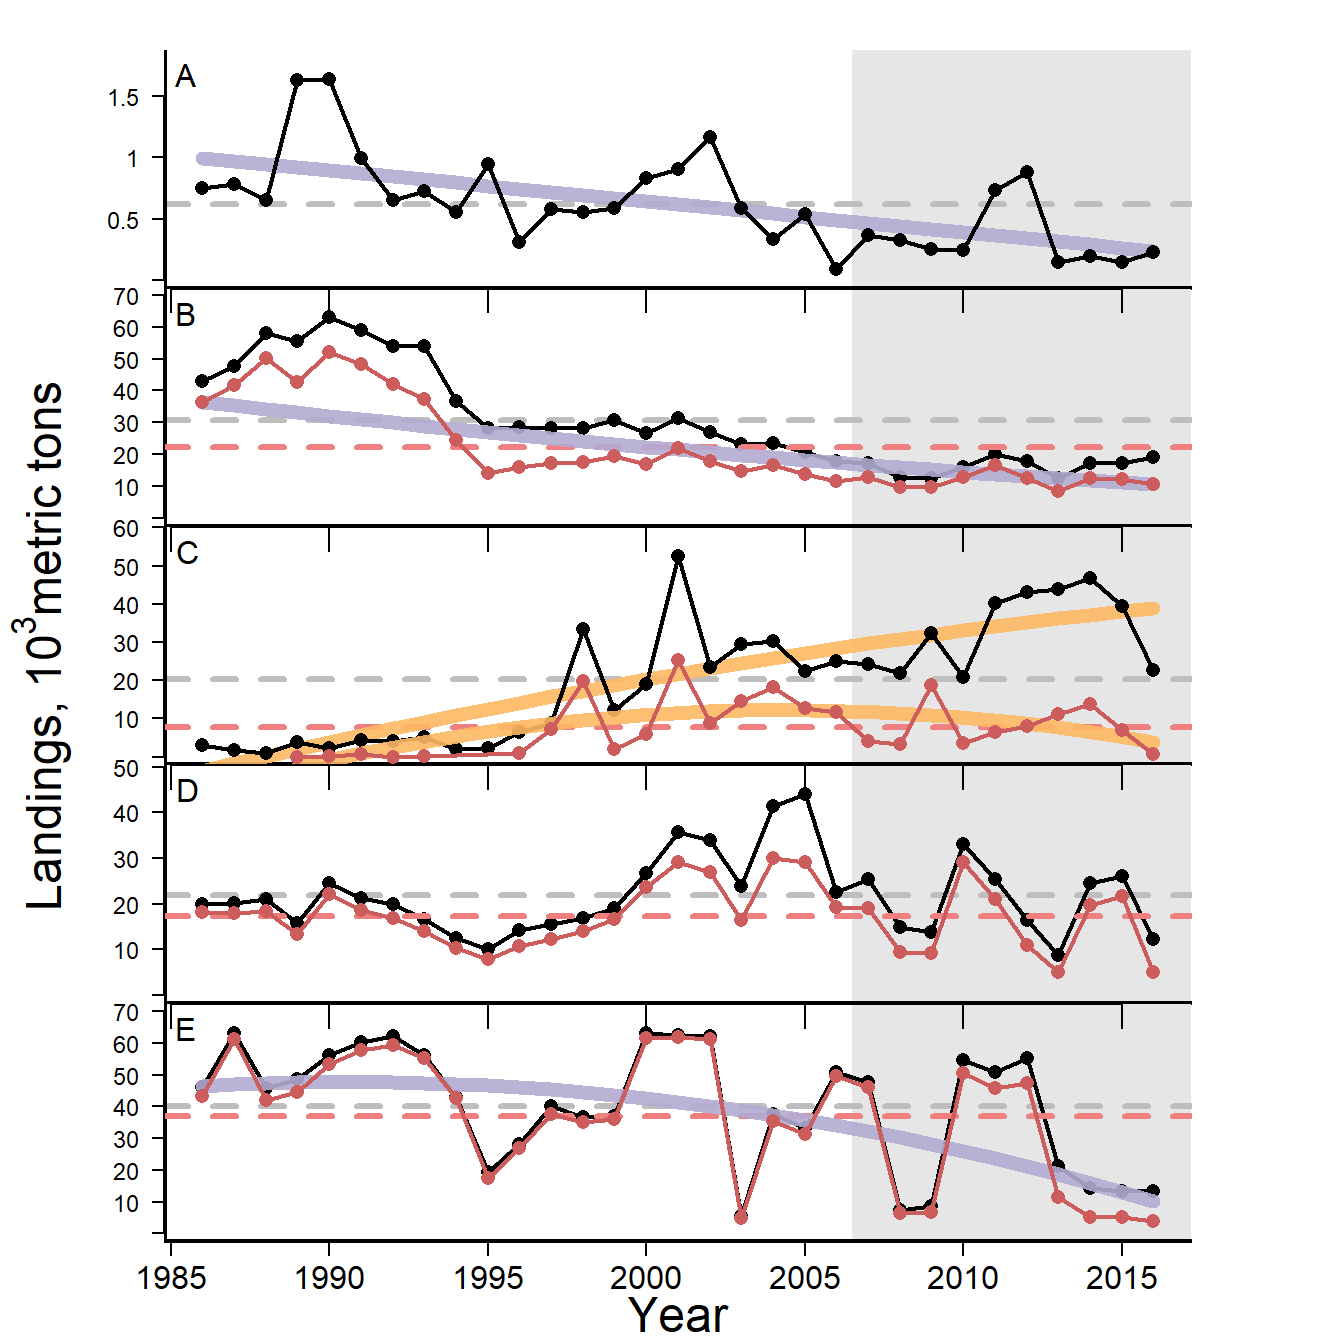
\includegraphics{C:/Users/kimberly.bastille/Desktop/tech-doc/imagesseafood-landings-1} 

}

\caption{NEFMC seafood specific landings (red) and total commericial landings (black) in Georges Bank (A: Apex predators, B: Piscivore, C: Planktivore, D: Benthivore, E: Benthos).}\label{fig:seafood-landings}
\end{figure}

\chapter{Long-term Sea Surface
Temperature}\label{long-term-sea-surface-temperature}

\textbf{Description}: Long-term sea-surface temperatures

\textbf{Found in}: State of the Ecosystem - Gulf of Maine \& Georges
Bank (2017, 2018, 2019), State of the Ecosystem - Mid-Atlantic (2017,
2018, 2019)

\textbf{Indicator category}: Database pull

\textbf{Contributor(s)}: Kevin Friedland

\textbf{Data steward}: Kevin Friedland,
\href{mailto:kevin.friedland@noaa.gov}{\nolinkurl{kevin.friedland@noaa.gov}}

\textbf{Point of contact}: Kevin Friedland,
\href{mailto:kevin.friedland@noaa.gov}{\nolinkurl{kevin.friedland@noaa.gov}}

\textbf{Public availability statement}: Source data are available
\href{https://www.esrl.noaa.gov/psd/data/gridded/data.noaa.ersst.v5.html}{here}.

\section{Methods}\label{methods-16}

Data for long-term sea-surface temperatures were derived from the NOAA
extended reconstructed sea surface temperature data set (ERSST V5). The
ERSST V5 dataset is parsed into 2° x 2° gridded bins between
1854-present with monthly temporal resolution. Data were interpolated in
regions with limited spatial coverage, and heavily damped during the
period between 1854-1880 when collection was inconsistent (Huang,
Thorne, et al.
\protect\hyperlink{ref-Huang2017}{2017}\protect\hyperlink{ref-Huang2017}{b};
Huang, Thorne, et al.
\protect\hyperlink{ref-huang2017extended}{2017}\protect\hyperlink{ref-huang2017extended}{a}).
For this analysis, 19 bins were selected that encompassed the Northeast
US Continental Shelf region (see Friedland and Hare
\protect\hyperlink{ref-Friedland2007}{2007}).

\subsection{Data sources}\label{data-sources-16}

This indicator is derived from the
\href{https://www.esrl.noaa.gov/psd/data/gridded/data.noaa.ersst.v5.html}{NOAA
ERSST V5 dataset} (Huang, Thorne, et al.
\protect\hyperlink{ref-Huang2017}{2017}\protect\hyperlink{ref-Huang2017}{b}).

\subsection{Data extraction}\label{data-extraction-14}

\label{tab:coordinates}Coordinates used in NOAA ERSST V5 data extraction.

Longitude

Latitude

-74

40

-74

38

-72

40

-70

44

-70

42

-70

40

-68

44

-68

42

R code used in extracting time series of long-term SST data.

\begin{Shaded}
\begin{Highlighting}[]
\CommentTok{# Include R code here}
\CommentTok{# all year}
\NormalTok{years=}\StringTok{"ersst"}

\CommentTok{# a year}
\CommentTok{#years=".2016"}

\CommentTok{# which data}
\KeywordTok{setwd}\NormalTok{(}\StringTok{"C:/2_ersst/datafiles_v4"}\NormalTok{)}
\KeywordTok{setwd}\NormalTok{(}\StringTok{"C:/2_ersst/datafiles_v5"}\NormalTok{)}


\CommentTok{# NES standard bounded by 34-46N and 78-62W}
\NormalTok{minlon=}\StringTok{ }\OperatorTok{-}\DecValTok{78}\NormalTok{; maxlon=}\StringTok{ }\OperatorTok{-}\DecValTok{62}\NormalTok{; minlat=}\StringTok{ }\DecValTok{34}\NormalTok{; maxlat=}\StringTok{ }\DecValTok{46}
\NormalTok{dataoutfile=}\StringTok{"C:/2_ersst/nes_std_area_v5.csv"}

\CommentTok{#  DELETE ONLY FILE WILL APPEND AND DOUBLE DATA}
\KeywordTok{file.remove}\NormalTok{(dataoutfile)}

\NormalTok{##################################################  }\RegionMarkerTok{END}\NormalTok{ SET}

\CommentTok{# LABRODOR SEA  }
\CommentTok{#minlon= -66; #maxlon= -44; #minlat= 50; #maxlat= 70}
\CommentTok{#dataoutfile="C:/2_ersst/lab_sea.csv"}

\CommentTok{# New eel}
\CommentTok{#minlon= -80; maxlon= -40; minlat= 20; maxlat= 40}
\CommentTok{#dataoutfile="C:/2_ersst/new eel.csv"}

\CommentTok{# G of Mex}
\CommentTok{#minlon= -98; maxlon= -82; minlat= 18; maxlat= 30}
\CommentTok{#dataoutfile="C:/2_ersst/gomex_area.csv"}

\CommentTok{# USSE INCLUDING  28-36N and 80-76W not bounding}
\CommentTok{#minlon= -80; #maxlon= -76; #minlat= 28; #maxlat= 36}
\CommentTok{#dataoutfile="C:/2_ersst/usse_area.csv"}

\CommentTok{# GSL standard bounded by 34-46N and 78-62W}
\CommentTok{#minlon= -68; maxlon= -60; minlat= 46; maxlat= 48}
\CommentTok{#dataoutfile="C:/2_ersst/gsl.csv"}

\CommentTok{# PACIFIC area bounded by 10-30N and 166-146W}
\CommentTok{#minlon= -166; #maxlon= -146; #minlat= 10; #maxlat= 30}
\CommentTok{#dataoutfile="C:/1_analyses/ersst/pac_islands_area.csv"}

\CommentTok{# Baltic area bounded by 52-66N and 14-28E}
\CommentTok{#minlon= 14; #maxlon= 28; #minlat= 52; #maxlat= 66}
\CommentTok{#dataoutfile="C:/2_ersst/baltic area.csv"}

\CommentTok{# North Atlantic Area bounded by 30-70N and 80W-20E}
\CommentTok{#minlon= -80; #maxlon= -2; #minlat= 30; #maxlat= 70}
\CommentTok{#dataoutfile="C:/2_ersst/na area1.csv"}
\CommentTok{# and ...}
\CommentTok{#minlon= 0; #maxlon= 20; #minlat= 30; #maxlat= 70}
\CommentTok{#dataoutfile="C:/1_analyses/ersst/na area2.csv"}

\CommentTok{# NorthEAST Atlantic Area bounded by 55-70N and 10W-20E}
\CommentTok{#minlon= -10; #maxlon= -2; #minlat= 56; #maxlat= 70}
\CommentTok{#dataoutfile="C:/1_analyses/ersst/ne atl 1.csv"}
\CommentTok{# and ...}
\CommentTok{#minlon= 0; #maxlon= 10; #minlat= 56; #maxlat= 70}
\CommentTok{#dataoutfile="C:/1_analyses/ersst/ne atl 2.csv"}

\CommentTok{# Pacific steelhead}
\CommentTok{#minlon= -160; #maxlon= -122; #minlat= 40; #maxlat= 62}
\CommentTok{#dataoutfile="C:/1_analyses/ersst/pac sh.csv"}

\CommentTok{#North Pacific in two parts}
\CommentTok{#1}
\CommentTok{#minlon= -180; #maxlon= -120; #minlat= 30; #maxlat= 72}
\CommentTok{#dataoutfile="C:/1_analyses/ersst/n_pac_1.csv"}
\CommentTok{#2}
\CommentTok{#minlon= 120; #maxlon= 178; #minlat= 30; #maxlat= 72}
\CommentTok{#dataoutfile="C:/1_analyses/ersst/n_pac_2.csv"}

\CommentTok{# North Atlantic Area bounded by 20-70N and 100W-30E}
\CommentTok{#minlon= -100; #maxlon= -2; #minlat= 20; #maxlat= 70}
\CommentTok{#dataoutfile="C:/1_analyses/ersst/na area1.csv"}
\CommentTok{# and ...}
\CommentTok{#minlon= 0; #maxlon= 30; #minlat= 20; #maxlat= 70}
\CommentTok{#dataoutfile="C:/1_analyses/ersst/na area2.csv"}









\CommentTok{# constants for area}
\NormalTok{R <-}\StringTok{ }\DecValTok{6371} \CommentTok{# Earth mean radius [km]}
\NormalTok{dheight =}\StringTok{  }\DecValTok{222}

\CommentTok{#library(ncdf)}
\KeywordTok{library}\NormalTok{(ncdf4)}

\CommentTok{# ERSST data  }
\CommentTok{# lon goes from 0E to 358E with lon at center of box}
\CommentTok{# lat goes from 88S to 88N with lat at center of box}

\CommentTok{# start with lon based on degrees lonew}
\CommentTok{# array  1  2  ...  90    91    92  ...  180}
\CommentTok{# lon    0  2  ... 178   180   182  ...  358}
\CommentTok{# lonew  0  2  ... 178  -180  -178  ...   -2}
\CommentTok{# star with lat + deg N, - deg S}
\CommentTok{# array    1  ...  45  ...  89}
\CommentTok{# lon    -88  ...   0  ...  88}

\CommentTok{# -> -> -> TO KEEP THINGS SIMPLE, RETRIEVALS CAN'T BE CONTINUOUS FROM - LONS TO + LONs}
\CommentTok{#          have to extract from -180W to -2W separately from 0E to 180E}

\CommentTok{# -> -> -> OUTPUT APPENDS SO NEED TO DELETE FILE IF ALREADY EXISTS}

\CommentTok{# -> -> -> USE APPROPRIATE lon lat and outfile block:}






\CommentTok{# set lon limits in array units}
\ControlFlowTok{if}\NormalTok{ ( minlon }\OperatorTok{<}\StringTok{ }\DecValTok{0}\NormalTok{)\{ }
\NormalTok{  arrayminlon=(minlon}\OperatorTok{+}\DecValTok{360}\NormalTok{)}\OperatorTok{/}\DecValTok{2}\OperatorTok{+}\DecValTok{1}
\NormalTok{\} }\ControlFlowTok{else}\NormalTok{ \{ }
\NormalTok{  arrayminlon=minlon}\OperatorTok{/}\DecValTok{2}\OperatorTok{+}\DecValTok{1} 
\NormalTok{\} }

\ControlFlowTok{if}\NormalTok{ ( maxlon }\OperatorTok{<}\StringTok{ }\DecValTok{0}\NormalTok{)\{ }
\NormalTok{  arraymaxlon=(maxlon}\OperatorTok{+}\DecValTok{360}\NormalTok{)}\OperatorTok{/}\DecValTok{2}\OperatorTok{+}\DecValTok{1}
\NormalTok{\} }\ControlFlowTok{else}\NormalTok{ \{ }
\NormalTok{  arraymaxlon=maxlon}\OperatorTok{/}\DecValTok{2}\OperatorTok{+}\DecValTok{1} 
\NormalTok{\} }

\CommentTok{# set lat limits in array units}
\NormalTok{arrayminlat=minlat}\OperatorTok{/}\DecValTok{2}\OperatorTok{+}\DecValTok{45}
\NormalTok{arraymaxlat=maxlat}\OperatorTok{/}\DecValTok{2}\OperatorTok{+}\DecValTok{45}


\NormalTok{filelist=}\KeywordTok{list.files}\NormalTok{(}\DataTypeTok{pattern=}\NormalTok{years)}

\NormalTok{numfiles=}\KeywordTok{length}\NormalTok{(filelist)}

\ControlFlowTok{for}\NormalTok{ (filenum }\ControlFlowTok{in} \DecValTok{1}\OperatorTok{:}\NormalTok{numfiles)\{}

\CommentTok{#  ersst = open.ncdf(filelist[filenum]) }
\NormalTok{  ersst =}\StringTok{ }\KeywordTok{nc_open}\NormalTok{(filelist[filenum]) }
  \KeywordTok{print}\NormalTok{(filelist[filenum])}

\CommentTok{#  sst = get.var.ncdf( ersst, "sst") }
\NormalTok{  sst <-}\StringTok{ }\KeywordTok{ncvar_get}\NormalTok{(ersst,}\StringTok{"sst"}\NormalTok{ )}
  
\NormalTok{  year=}\KeywordTok{as.numeric}\NormalTok{(}\KeywordTok{substr}\NormalTok{(filelist[filenum],}\DecValTok{10}\NormalTok{,}\DecValTok{13}\NormalTok{))}
\NormalTok{  month=}\KeywordTok{as.numeric}\NormalTok{(}\KeywordTok{substr}\NormalTok{(filelist[filenum],}\DecValTok{14}\NormalTok{,}\DecValTok{15}\NormalTok{))}

  \ControlFlowTok{for}\NormalTok{ (arrlons }\ControlFlowTok{in}\NormalTok{ arrayminlon}\OperatorTok{:}\NormalTok{arraymaxlon)\{}
    \ControlFlowTok{for}\NormalTok{ (arrlats }\ControlFlowTok{in}\NormalTok{ arrayminlat}\OperatorTok{:}\NormalTok{arraymaxlat)\{}
      

      \ControlFlowTok{if}\NormalTok{ ( arrlons }\OperatorTok{<}\StringTok{ }\DecValTok{91}\NormalTok{)\{ }
\NormalTok{        regenlon=(arrlons}\OperatorTok{-}\DecValTok{1}\NormalTok{)}\OperatorTok{*}\DecValTok{2}
\NormalTok{      \} }\ControlFlowTok{else}\NormalTok{ \{ }
\NormalTok{        regenlon=(arrlons}\OperatorTok{-}\DecValTok{1}\NormalTok{)}\OperatorTok{*}\DecValTok{2}\OperatorTok{-}\DecValTok{360}
\NormalTok{      \} }
      
    
\NormalTok{      regenlat=(arrlats}\OperatorTok{-}\DecValTok{45}\NormalTok{)}\OperatorTok{*}\DecValTok{2}
      
\NormalTok{      long1=regenlon}\OperatorTok{-}\DecValTok{1} \OperatorTok{*}\NormalTok{pi}\OperatorTok{/}\DecValTok{180}
\NormalTok{      lat1=regenlat}\OperatorTok{-}\DecValTok{1} \OperatorTok{*}\NormalTok{pi}\OperatorTok{/}\DecValTok{180}
\NormalTok{      long2=regenlon}\OperatorTok{+}\DecValTok{1} \OperatorTok{*}\NormalTok{pi}\OperatorTok{/}\DecValTok{180}
\NormalTok{      lat2=regenlat}\OperatorTok{-}\DecValTok{1} \OperatorTok{*}\NormalTok{pi}\OperatorTok{/}\DecValTok{180}
\NormalTok{      dwidth1 <-}\StringTok{ }\KeywordTok{acos}\NormalTok{(}\KeywordTok{sin}\NormalTok{(lat1)}\OperatorTok{*}\KeywordTok{sin}\NormalTok{(lat2) }\OperatorTok{+}\StringTok{ }\KeywordTok{cos}\NormalTok{(lat1)}\OperatorTok{*}\KeywordTok{cos}\NormalTok{(lat2) }\OperatorTok{*}\StringTok{ }\KeywordTok{cos}\NormalTok{(long2}\OperatorTok{-}\NormalTok{long1)) }\OperatorTok{*}\StringTok{ }\NormalTok{R}
\NormalTok{      long1=regenlon}\OperatorTok{-}\DecValTok{1} \OperatorTok{*}\NormalTok{pi}\OperatorTok{/}\DecValTok{180}
\NormalTok{      lat1=regenlat}\OperatorTok{+}\DecValTok{1} \OperatorTok{*}\NormalTok{pi}\OperatorTok{/}\DecValTok{180}
\NormalTok{      long2=regenlon}\OperatorTok{+}\DecValTok{1} \OperatorTok{*}\NormalTok{pi}\OperatorTok{/}\DecValTok{180}
\NormalTok{      lat2=regenlat}\OperatorTok{+}\DecValTok{1} \OperatorTok{*}\NormalTok{pi}\OperatorTok{/}\DecValTok{180}
\NormalTok{      dwidth2 <-}\StringTok{ }\KeywordTok{acos}\NormalTok{(}\KeywordTok{sin}\NormalTok{(lat1)}\OperatorTok{*}\KeywordTok{sin}\NormalTok{(lat2) }\OperatorTok{+}\StringTok{ }\KeywordTok{cos}\NormalTok{(lat1)}\OperatorTok{*}\KeywordTok{cos}\NormalTok{(lat2) }\OperatorTok{*}\StringTok{ }\KeywordTok{cos}\NormalTok{(long2}\OperatorTok{-}\NormalTok{long1)) }\OperatorTok{*}\StringTok{ }\NormalTok{R}
\NormalTok{      area=((dwidth1 }\OperatorTok{+}\StringTok{ }\NormalTok{dwidth1)}\OperatorTok{/}\DecValTok{2}\NormalTok{) }\OperatorTok{*}\StringTok{ }\NormalTok{dheight}
      
\NormalTok{      dataline <-}\StringTok{ }\KeywordTok{matrix}\NormalTok{(}\KeywordTok{c}\NormalTok{(year, month, regenlon, regenlat, }\KeywordTok{round}\NormalTok{(sst[arrlons,arrlats],}\DataTypeTok{digits=}\DecValTok{2}\NormalTok{),area),}\DecValTok{1}\NormalTok{,}\DecValTok{6}\NormalTok{)}
      
      
      \ControlFlowTok{if}\NormalTok{(}\KeywordTok{is.finite}\NormalTok{(sst[arrlons,arrlats])) \{}
      \KeywordTok{write.table}\NormalTok{(dataline,}\DataTypeTok{file=}\NormalTok{dataoutfile,}\DataTypeTok{sep=}\StringTok{","}\NormalTok{,}\DataTypeTok{row.name=}\NormalTok{F,}\DataTypeTok{col.names=}\NormalTok{F,}\DataTypeTok{append=}\OtherTok{TRUE}\NormalTok{)   }
\NormalTok{    \}}
      
\NormalTok{    \}}
\NormalTok{  \}}

\CommentTok{#    close.ncdf(ersst) }
\KeywordTok{nc_close}\NormalTok{(ersst)}
  
\NormalTok{  \}}
\end{Highlighting}
\end{Shaded}

\subsection{Data Processing}\label{data-processing-10}

Data were formatted for inclusion in the ecodata R package with the
following R code.

\begin{Shaded}
\begin{Highlighting}[]
\CommentTok{#process ERSST long-term SST data}

\KeywordTok{library}\NormalTok{(dplyr)}
\KeywordTok{library}\NormalTok{(tidyr)}

\NormalTok{raw.dir <-}\StringTok{ }\NormalTok{here}\OperatorTok{::}\KeywordTok{here}\NormalTok{(}\StringTok{"data-raw"}\NormalTok{)}

\NormalTok{get_long_term_sst <-}\StringTok{ }\ControlFlowTok{function}\NormalTok{(}\DataTypeTok{save_clean =}\NormalTok{ F)\{}
\NormalTok{  long_term_sst <-}\StringTok{ }\KeywordTok{read.csv}\NormalTok{(}\KeywordTok{file.path}\NormalTok{(raw.dir,}\StringTok{"ersst annual mean.csv"}\NormalTok{)) }\OperatorTok\StringTok{ }
\StringTok{    }\NormalTok{dplyr}\OperatorTok{::}\KeywordTok{rename}\NormalTok{(}\DataTypeTok{Time =}\NormalTok{ Year,}
                  \DataTypeTok{Value =}\NormalTok{ Mean) }\OperatorTok\StringTok{ }
\StringTok{    }\KeywordTok{mutate}\NormalTok{(}\DataTypeTok{Var =} \StringTok{"long-term sst"}\NormalTok{,}
           \DataTypeTok{EPU =} \StringTok{"All"}\NormalTok{,}
           \DataTypeTok{Units =} \StringTok{"degreesC"}\NormalTok{)}
  
  \ControlFlowTok{if}\NormalTok{ (save_clean) \{}
\NormalTok{    usethis}\OperatorTok{::}\KeywordTok{use_data}\NormalTok{(long_term_sst, }\DataTypeTok{overwrite =}\NormalTok{ T)}
\NormalTok{  \} }\ControlFlowTok{else}\NormalTok{ \{}
    \KeywordTok{return}\NormalTok{(long_term_sst)}
\NormalTok{  \}}
  
\NormalTok{\}}
\end{Highlighting}
\end{Shaded}

\subsection{Plotting}\label{plotting-11}

\begin{Shaded}
\begin{Highlighting}[]
\CommentTok{# Relative working directories}
\NormalTok{data.dir  <-}\StringTok{ }\NormalTok{here}\OperatorTok{::}\KeywordTok{here}\NormalTok{(}\StringTok{'data'}\NormalTok{)}
\NormalTok{r.dir <-}\StringTok{ }\NormalTok{here}\OperatorTok{::}\KeywordTok{here}\NormalTok{(}\StringTok{'R'}\NormalTok{)}

\CommentTok{# Load data}
\KeywordTok{load}\NormalTok{(}\KeywordTok{file.path}\NormalTok{(data.dir,}\StringTok{"SOE_data_erddap.Rdata"}\NormalTok{))}

\CommentTok{# Source plotting functions}
\KeywordTok{source}\NormalTok{(}\KeywordTok{file.path}\NormalTok{(r.dir,}\StringTok{"BasePlot_source.R"}\NormalTok{))}


\NormalTok{opar <-}\StringTok{ }\KeywordTok{par}\NormalTok{(}\DataTypeTok{mar =} \KeywordTok{c}\NormalTok{(}\DecValTok{4}\NormalTok{, }\DecValTok{6}\NormalTok{, }\DecValTok{2}\NormalTok{, }\DecValTok{6}\NormalTok{))}
\KeywordTok{soe.plot}\NormalTok{(SOE.data, }\StringTok{"Time"}\NormalTok{, }\StringTok{"long term sst"}\NormalTok{, }\DataTypeTok{end.start =} \DecValTok{2007}\NormalTok{, }
         \DataTypeTok{line.forward =} \OtherTok{TRUE}\NormalTok{, }\DataTypeTok{point.cex =} \FloatTok{0.8}\NormalTok{, }\DataTypeTok{rel.y.text =} \FloatTok{1.1}\NormalTok{,}
         \DataTypeTok{x.line =} \DecValTok{2}\NormalTok{, }\DataTypeTok{y.line =} \FloatTok{2.3}\NormalTok{, }\DataTypeTok{x.label =} \StringTok{'Year'}\NormalTok{, }\DataTypeTok{rel.y.num =} \FloatTok{1.1}\NormalTok{,}
         \DataTypeTok{y.label =} \KeywordTok{expression}\NormalTok{(}\KeywordTok{paste}\NormalTok{(}\StringTok{"Mean SST ("}\NormalTok{,degree,}\StringTok{"C)"}\NormalTok{)))}
\end{Highlighting}
\end{Shaded}

\begin{figure}

{\centering 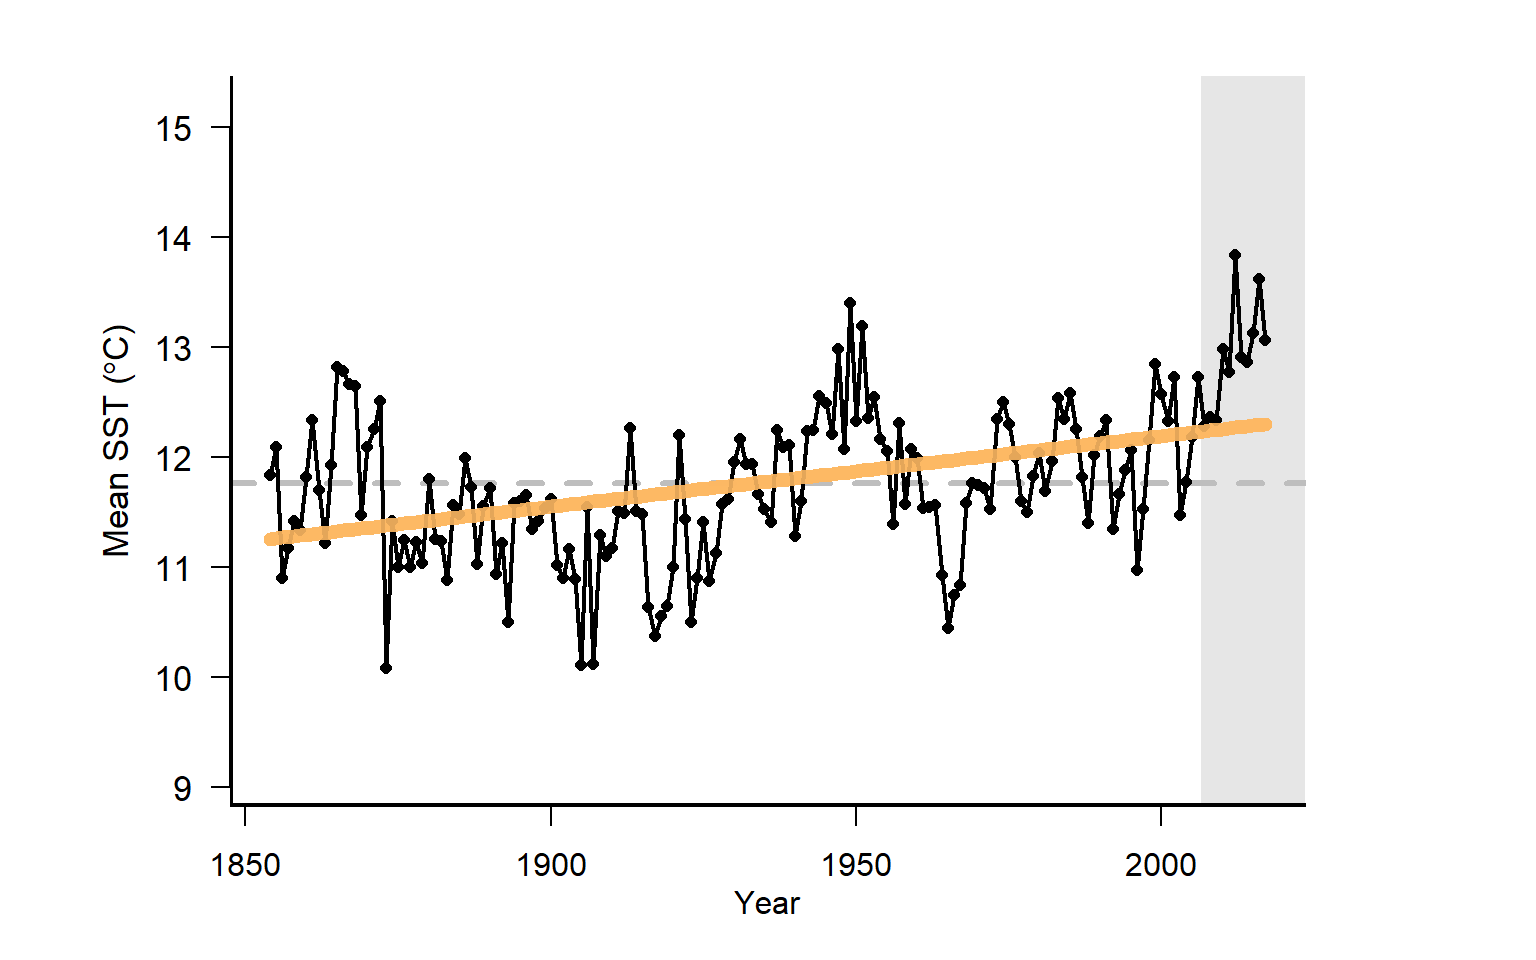
\includegraphics{C:/Users/kimberly.bastille/Desktop/tech-doc/imageslong-term-sst-1} 

}

\caption{Long-term sea surface temperatures on the Northeast Continental Shelf.}\label{fig:long-term-sst}
\end{figure}

\chapter{Mid-Atlantic Harmful Algal Bloom
Indicator}\label{mid-atlantic-harmful-algal-bloom-indicator}

\textbf{Description}: An aggregation of reported algal bloom data in
Chesapeake Bay between 2007-2017.

\textbf{Found in}: State of the Ecosystem - Mid-Atlantic (2018)

\textbf{Indicator category}: Database pull

\textbf{Contributor(s)}: Sean Hardison, Virginia Department of Health

\textbf{Data steward}: Sean Hardison,
\href{mailto:sean.hardison@noaa.gov}{\nolinkurl{sean.hardison@noaa.gov}}

\textbf{Point of contact}: Sean Hardison,
\href{mailto:sean.hardison@noaa.gov}{\nolinkurl{sean.hardison@noaa.gov}}

\textbf{Public availability statement}: Source data for this indicator
are available
\href{https://github.com/NOAA-EDAB/tech-doc/tree/master/data/CB_HAB}{here}.
Processed time series can be found
\href{http://comet.nefsc.noaa.gov/erddap/tabledap/CBhabs_ann_soe_v2.html}{here}.

\section{Methods}\label{methods-17}

We presented two indicator time series for reports of algal blooms in
the southern portion of Chesapeake Bay between 2007-2017. The first
indicator was observations of algal blooms above 5000 cell
ml\textsuperscript{-1}. This threshold was developed by the Virginia
Department of Health (VDH) for \emph{Microcystis} spp. algal blooms
based on World Health Organization guidelines (Organization
\protect\hyperlink{ref-WHO2003}{2003}; Health
\protect\hyperlink{ref-VDH2011}{2011}). VDH also uses this same
threshold for other algal species blooms in Virginia waters. When cell
concentrations are above 5000 cell ml\textsuperscript{-1}, VDH
recommends initiation of biweekly water sampling and that relevant local
agencies be notified of the elevated cell concentrations.

The second indicator we reported, blooms of \emph{Cochlodinium
polykrikoides} at cell concentrations \textgreater{}300 cell
ml\textsuperscript{-1}, was chosen due to reports of high
ichthyotoxicity seen at these levels. Tang and Gobler
(\protect\hyperlink{ref-Tang2009}{2009}) showed that fish exposed to
cultured \emph{C. polykrikoides} at densities as low 330 cells
ml\textsuperscript{-1} saw 100\% mortality within 1 hour, which if often
far less than \emph{C. polykrikoides} cell concentrations seen in the
field. Algal bloom data were not available for 2015 nor 2010. The algal
bloom information presented here are a synthesis of reported events, and
has been updated to include data not presented in the 2018 State of the
Ecosystem Report.

\subsection{Data sources}\label{data-sources-17}

Source data were obtained from VDH. Sampling, identification, and bloom
characterization was completed by the VDH, Phytoplankton Analysis
Laboratory at Old Dominion University, Reece Lab at the Virginia
Institute of Marine Science, and Virginia Department of Environmental
Quality. Problem algal species were targeted for identification via
light microscopy followed by standard or quantitative PCR assays and/or
enzyme-linked immunosorbent assay (ELISA). Reports specifying full
methodologies from ODU, VIMS, and VDH source data are available upon
request.

\subsection{Data extraction}\label{data-extraction-15}

Data were extracted from a series of spreadsheets provided by the VDH.
We quantified the number of algal blooms in each year reaching target
cell density thresholds in the southern Chesapeake Bay.

\begin{Shaded}
\begin{Highlighting}[]
\CommentTok{#SOE R packages}

\KeywordTok{library}\NormalTok{(readxl)}
\KeywordTok{library}\NormalTok{(dplyr)}
\KeywordTok{library}\NormalTok{(tidyr)}
\KeywordTok{library}\NormalTok{(stringr)}
\end{Highlighting}
\end{Shaded}

\begin{Shaded}
\begin{Highlighting}[]
\NormalTok{data.dir <-}\StringTok{ "data/CB_HAB"}

\CommentTok{#Function to process data - cpm specifies cells per ml filter}
\NormalTok{fixer <-}\StringTok{ }\ControlFlowTok{function}\NormalTok{(cpm)\{}
\NormalTok{  hab_2007_}\DecValTok{2012}\NormalTok{ <-}\StringTok{ }\KeywordTok{read_excel}\NormalTok{(}\KeywordTok{file.path}\NormalTok{(data.dir,}\StringTok{"Query_2007-2012.xlsx"}\NormalTok{))}
\NormalTok{  hab_2013_odu <-}\StringTok{ }\KeywordTok{read_excel}\NormalTok{(}\KeywordTok{file.path}\NormalTok{(data.dir,}\StringTok{"2013 ODU Data.xlsx"}\NormalTok{),}\DataTypeTok{skip =} \DecValTok{4}\NormalTok{)}
\NormalTok{  hab_2013_vims <-}\StringTok{ }\KeywordTok{read_excel}\NormalTok{(}\KeywordTok{file.path}\NormalTok{(data.dir,}\StringTok{"vims_2013.xlsx"}\NormalTok{),}\DataTypeTok{skip =} \DecValTok{6}\NormalTok{)}
\NormalTok{  hab_2014_odu <-}\StringTok{ }\KeywordTok{read_excel}\NormalTok{(}\KeywordTok{file.path}\NormalTok{(data.dir,}\StringTok{"2014 ODU data.xlsx"}\NormalTok{))}
\NormalTok{  hab_2014_vims <-}\StringTok{ }\KeywordTok{read_excel}\NormalTok{(}\KeywordTok{file.path}\NormalTok{(data.dir,}\StringTok{"FINALforVDH_22Dec14final.xlsx"}\NormalTok{))}
\NormalTok{  hab_}\DecValTok{2016}\NormalTok{ <-}\StringTok{ }\KeywordTok{read_excel}\NormalTok{(}\KeywordTok{file.path}\NormalTok{(data.dir,}\StringTok{"HAB_MAP_Data_2016.xlsx"}\NormalTok{))}
\NormalTok{  hab_}\DecValTok{2017}\NormalTok{ <-}\StringTok{ }\KeywordTok{read_excel}\NormalTok{(}\KeywordTok{file.path}\NormalTok{(data.dir,}\StringTok{"HAB_MAP_Data_2017.xlsx"}\NormalTok{),}\DataTypeTok{sheet=}\DecValTok{2}\NormalTok{)}
  
  \CommentTok{#2012---------------------------------------------------------}
\NormalTok{  HAB_2007_}\DecValTok{2012}\NormalTok{ <-}\StringTok{ }\NormalTok{hab_2007_}\DecValTok{2012} \OperatorTok\StringTok{ }\KeywordTok{filter}\NormalTok{(}\OperatorTok{!}\KeywordTok{is.na}\NormalTok{(cells_per_ml)) }\OperatorTok
\StringTok{    }\KeywordTok{filter}\NormalTok{(}\OperatorTok{!}\KeywordTok{is.na}\NormalTok{(date)) }\OperatorTok
\StringTok{    }\KeywordTok{mutate}\NormalTok{(}\DataTypeTok{year =} \KeywordTok{format}\NormalTok{(}\KeywordTok{as.POSIXct}\NormalTok{(date), }\StringTok{"%Y"}\NormalTok{)) }\OperatorTok\StringTok{ }
\StringTok{    }\KeywordTok{filter}\NormalTok{(cells_per_ml }\OperatorTok{>=}\StringTok{ }\NormalTok{cpm) }\OperatorTok
\StringTok{    }\KeywordTok{group_by}\NormalTok{(year, species) }\OperatorTok
\StringTok{    }\NormalTok{dplyr}\OperatorTok{::}\KeywordTok{summarise}\NormalTok{(}\DataTypeTok{Events =} \KeywordTok{n}\NormalTok{()) }\OperatorTok
\StringTok{    }\KeywordTok{as.data.frame}\NormalTok{()}
  
  \CommentTok{#2013---------------------------------------------------------}
  \CommentTok{#ODU}
\NormalTok{  odu_}\DecValTok{2013}\NormalTok{ <-}\StringTok{ }\KeywordTok{gather}\NormalTok{(hab_2013_odu, species, cells_per_ml, }\StringTok{`}\DataTypeTok{Pfiesteria like dinoflagellate}\StringTok{`}\OperatorTok{:}\StringTok{`}\DataTypeTok{A. monilatum}\StringTok{`}\NormalTok{) }\OperatorTok
\StringTok{    }\KeywordTok{filter}\NormalTok{(}\OperatorTok{!}\KeywordTok{is.na}\NormalTok{(cells_per_ml)) }\OperatorTok
\StringTok{    }\KeywordTok{filter}\NormalTok{(cells_per_ml }\OperatorTok{>=}\StringTok{ }\NormalTok{cpm) }\OperatorTok
\StringTok{    }\KeywordTok{mutate}\NormalTok{(}\DataTypeTok{year =} \DecValTok{2013}\NormalTok{) }\OperatorTok
\StringTok{    }\KeywordTok{group_by}\NormalTok{(year, species) }\OperatorTok
\StringTok{    }\NormalTok{dplyr}\OperatorTok{::}\KeywordTok{summarise}\NormalTok{(}\DataTypeTok{Events =} \KeywordTok{n}\NormalTok{()) }\OperatorTok
\StringTok{    }\KeywordTok{as.data.frame}\NormalTok{()}
  
  \CommentTok{#VIMS}
\NormalTok{  vims_}\DecValTok{2013}\NormalTok{ <-}\StringTok{ }\NormalTok{hab_2013_vims }\OperatorTok\StringTok{ }\KeywordTok{filter}\NormalTok{(}\OperatorTok{!}\KeywordTok{is.na}\NormalTok{(cells_per_ml)) }\OperatorTok
\StringTok{    }\KeywordTok{mutate}\NormalTok{(}\DataTypeTok{year =} \StringTok{"2013"}\NormalTok{) }\OperatorTok
\StringTok{    }\KeywordTok{filter}\NormalTok{(cells_per_ml }\OperatorTok{>=}\StringTok{ }\NormalTok{cpm) }\OperatorTok
\StringTok{    }\KeywordTok{group_by}\NormalTok{(year, species) }\OperatorTok
\StringTok{    }\NormalTok{dplyr}\OperatorTok{::}\KeywordTok{summarise}\NormalTok{(}\DataTypeTok{Events =} \KeywordTok{n}\NormalTok{()) }\OperatorTok
\StringTok{    }\KeywordTok{as.data.frame}\NormalTok{()}
  
\NormalTok{  HAB_}\DecValTok{2013}\NormalTok{ <-}\StringTok{ }\KeywordTok{rbind}\NormalTok{(vims_}\DecValTok{2013}\NormalTok{, odu_}\DecValTok{2013}\NormalTok{)}
  
  \CommentTok{#2014--------------------------------------------------------}
  \CommentTok{#ODU}
\NormalTok{  long <-}\StringTok{ }\KeywordTok{gather}\NormalTok{(hab_2014_odu, species, cells_per_ml, }\StringTok{`}\DataTypeTok{Karlodinium veneficum}\StringTok{`}\OperatorTok{:}\StringTok{`}\DataTypeTok{Cyanobacteria bloom}\StringTok{`}\NormalTok{, }\DataTypeTok{factor_key =} \OtherTok{TRUE}\NormalTok{)}
\NormalTok{  hab_2014_odu <-}\StringTok{ }\NormalTok{long }\OperatorTok\StringTok{ }\KeywordTok{filter}\NormalTok{(cells_per_ml }\OperatorTok{!=}\StringTok{ }\DecValTok{0}\NormalTok{)}
\NormalTok{  hab_2014_odu}\OperatorTok{$}\NormalTok{species <-}\StringTok{ }\KeywordTok{sub}\NormalTok{(}\StringTok{"[.]"}\NormalTok{,}\StringTok{" "}\NormalTok{, hab_2014_odu}\OperatorTok{$}\NormalTok{species)}
\NormalTok{  hab_2014_odu}\OperatorTok{$}\NormalTok{cells_per_ml <-}\StringTok{ }\KeywordTok{gsub}\NormalTok{(}\StringTok{"[A-Za-z+//]"}\NormalTok{,}\StringTok{''}\NormalTok{,hab_2014_odu}\OperatorTok{$}\NormalTok{cells_per_ml)}
\NormalTok{  hab_2014_odu}\OperatorTok{$}\NormalTok{cells_per_ml <-}\StringTok{ }\KeywordTok{as.numeric}\NormalTok{(hab_2014_odu}\OperatorTok{$}\NormalTok{cells_per_ml)}
  
\NormalTok{  hab_2014_odu <-}\StringTok{ }\NormalTok{hab_2014_odu }\OperatorTok\StringTok{ }\KeywordTok{mutate}\NormalTok{(}\DataTypeTok{year =} \StringTok{"2014"}\NormalTok{) }\OperatorTok
\StringTok{    }\KeywordTok{filter}\NormalTok{(cells_per_ml }\OperatorTok{>=}\StringTok{ }\NormalTok{cpm) }\OperatorTok
\StringTok{    }\KeywordTok{group_by}\NormalTok{(year,species) }\OperatorTok
\StringTok{    }\NormalTok{dplyr}\OperatorTok{::}\KeywordTok{summarise}\NormalTok{(}\DataTypeTok{Events =} \KeywordTok{n}\NormalTok{()) }\OperatorTok
\StringTok{    }\KeywordTok{as.data.frame}\NormalTok{()}
  
  \CommentTok{#VIMS}
\NormalTok{  long <-}\StringTok{ }\KeywordTok{gather}\NormalTok{(hab_2014_vims, species, cells_per_ml, }\StringTok{`}\DataTypeTok{A. monilatum}\StringTok{`}\OperatorTok{:}\StringTok{`}\DataTypeTok{C. subsalsa}\StringTok{`}\NormalTok{)}
\NormalTok{  hab_2014_vims <-}\StringTok{ }\NormalTok{long }\OperatorTok\StringTok{ }\KeywordTok{mutate}\NormalTok{(}\DataTypeTok{year =} \StringTok{"2014"}\NormalTok{) }\OperatorTok\StringTok{ }\KeywordTok{filter}\NormalTok{(}\OperatorTok{!}\KeywordTok{is.na}\NormalTok{(cells_per_ml)) }\OperatorTok
\StringTok{    }\KeywordTok{mutate}\NormalTok{(}\DataTypeTok{cells_per_ml =} \KeywordTok{as.numeric}\NormalTok{(cells_per_ml)) }\OperatorTok\StringTok{ }
\StringTok{    }\KeywordTok{filter}\NormalTok{(cells_per_ml }\OperatorTok{>=}\StringTok{ }\NormalTok{cpm) }\OperatorTok
\StringTok{    }\KeywordTok{group_by}\NormalTok{(year,species) }\OperatorTok
\StringTok{    }\NormalTok{dplyr}\OperatorTok{::}\KeywordTok{summarise}\NormalTok{(}\DataTypeTok{Events =} \KeywordTok{n}\NormalTok{()) }\OperatorTok
\StringTok{    }\KeywordTok{as.data.frame}\NormalTok{()}
\NormalTok{  HAB_}\DecValTok{2014}\NormalTok{ <-}\StringTok{ }\KeywordTok{rbind}\NormalTok{(hab_2014_odu, hab_2014_vims)}
  
  \CommentTok{#2015----------------------------------------------------------}
  \CommentTok{#No data}
  
  \CommentTok{#2016---------------------------------------------------------}
\NormalTok{  HAB_}\DecValTok{2016}\NormalTok{ <-}\StringTok{ }\NormalTok{hab_}\DecValTok{2016} \OperatorTok\StringTok{ }\KeywordTok{mutate}\NormalTok{(}\DataTypeTok{species=} 
\NormalTok{                                    plyr}\OperatorTok{::}\KeywordTok{mapvalues}\NormalTok{(species, }
                                                    \DataTypeTok{from =} \KeywordTok{c}\NormalTok{(}\StringTok{"Eugelna sanguinea"}\NormalTok{,}
                                                             \StringTok{"Microcystin aeruginosa"}\NormalTok{,}
                                                             \StringTok{"Microcystis aeruginosa"}\NormalTok{,}
                                                             \StringTok{"Alexandrium monilatum-likely"}\NormalTok{,}
                                                             \StringTok{"Alexandrium monilatum"}\NormalTok{),}
                                                    \DataTypeTok{to =} \KeywordTok{c}\NormalTok{(}\StringTok{"Eugelena spp."}\NormalTok{, }
                                                           \StringTok{"Microcystis spp."}\NormalTok{,}
                                                           \StringTok{"Microcystis spp."}\NormalTok{,}
                                                           \StringTok{"Alexandrium spp."}\NormalTok{,}
                                                           \StringTok{"Alexandrium spp."}\NormalTok{)))}
\NormalTok{  HAB_}\DecValTok{2016}\OperatorTok{$}\NormalTok{cells_per_ml <-}\StringTok{ }\KeywordTok{gsub}\NormalTok{(}\StringTok{'[a-zA-Z+<>]'}\NormalTok{,}\StringTok{''}\NormalTok{,HAB_}\DecValTok{2016}\OperatorTok{$}\NormalTok{cells_per_ml)}
\NormalTok{  HAB_}\DecValTok{2016}\NormalTok{ <-}\StringTok{ }\NormalTok{HAB_}\DecValTok{2016} \OperatorTok
\StringTok{    }\KeywordTok{filter}\NormalTok{(}\OperatorTok{!}\KeywordTok{is.na}\NormalTok{(cells_per_ml)) }\OperatorTok
\StringTok{    }\KeywordTok{mutate}\NormalTok{(}\DataTypeTok{year =} \DecValTok{2016}\NormalTok{, }\DataTypeTok{cells_per_ml =} \KeywordTok{as.numeric}\NormalTok{(cells_per_ml)) }\OperatorTok
\StringTok{    }\KeywordTok{filter}\NormalTok{(cells_per_ml }\OperatorTok{>=}\StringTok{ }\NormalTok{cpm) }\OperatorTok
\StringTok{    }\KeywordTok{group_by}\NormalTok{(year, species) }\OperatorTok
\StringTok{    }\NormalTok{dplyr}\OperatorTok{::}\KeywordTok{summarise}\NormalTok{(}\DataTypeTok{Events =} \KeywordTok{n}\NormalTok{()) }\OperatorTok
\StringTok{    }\KeywordTok{as.data.frame}\NormalTok{()}
  
  \CommentTok{#2017------------------------------------------------------------}
\NormalTok{  hab_}\DecValTok{2017}\OperatorTok{$}\NormalTok{species =}\StringTok{ }\KeywordTok{str_trim}\NormalTok{(hab_}\DecValTok{2017}\OperatorTok{$}\NormalTok{species)}
\NormalTok{  HAB_}\DecValTok{2017}\NormalTok{ <-}\StringTok{ }\NormalTok{hab_}\DecValTok{2017} \OperatorTok\StringTok{ }\KeywordTok{mutate}\NormalTok{(}\DataTypeTok{species =}\NormalTok{ plyr}\OperatorTok{::}\KeywordTok{mapvalues}\NormalTok{(species, }\KeywordTok{c}\NormalTok{(}\StringTok{"A. monilatum"}\NormalTok{,}\StringTok{"Anabaena sp"}\NormalTok{,}
                                                                       \StringTok{"Anabaena sp."}\NormalTok{,}\StringTok{"Anabaena spp"}\NormalTok{,}
                                                                       \StringTok{"none"}\NormalTok{,}\StringTok{"NO HABs"}\NormalTok{,}\StringTok{"C. polykrikoides"}\NormalTok{,}
                                                                       \StringTok{"Microcystis aeurignosa"}\NormalTok{,}\StringTok{"Cylindrospermopsis sp"}\NormalTok{),}
                                                            \KeywordTok{c}\NormalTok{(}\StringTok{"Alexandrium monilatum"}\NormalTok{, }\StringTok{"Anabaena spp."}\NormalTok{,}
                                                              \StringTok{"Anabaena spp."}\NormalTok{,}\StringTok{"Anabaena spp."}\NormalTok{,}
                                                              \StringTok{"NA"}\NormalTok{,}\StringTok{"NA"}\NormalTok{,}\StringTok{"Cochlodinium polykrikoides"}\NormalTok{,}
                                                              \StringTok{"Microcystis aeruginosa"}\NormalTok{,}\StringTok{"Cylindrospermopsis sp."}\NormalTok{)))}
\NormalTok{  HAB_}\DecValTok{2017}\OperatorTok{$}\NormalTok{cells_per_ml <-}\StringTok{ }\KeywordTok{gsub}\NormalTok{(}\StringTok{"[a-zA-Z+/]"}\NormalTok{,}\StringTok{''}\NormalTok{,HAB_}\DecValTok{2017}\OperatorTok{$}\NormalTok{cells_per_ml)}
\NormalTok{  HAB_}\DecValTok{2017}\OperatorTok{$}\NormalTok{cells_per_ml <-}\StringTok{ }\KeywordTok{str_trim}\NormalTok{(HAB_}\DecValTok{2017}\OperatorTok{$}\NormalTok{cells_per_ml)}
\NormalTok{  HAB_}\DecValTok{2017}\OperatorTok{$}\NormalTok{cells_per_ml <-}\StringTok{ }\KeywordTok{as.numeric}\NormalTok{(HAB_}\DecValTok{2017}\OperatorTok{$}\NormalTok{cells_per_ml)}
\NormalTok{  HAB_}\DecValTok{2017}\NormalTok{ <-}\StringTok{ }\NormalTok{HAB_}\DecValTok{2017} \OperatorTok\StringTok{ }
\StringTok{    }\KeywordTok{filter}\NormalTok{(}\OperatorTok{!}\KeywordTok{is.na}\NormalTok{(cells_per_ml)) }\OperatorTok
\StringTok{    }\KeywordTok{mutate}\NormalTok{(}\DataTypeTok{year =} \StringTok{"2017"}\NormalTok{) }\OperatorTok
\StringTok{    }\KeywordTok{filter}\NormalTok{(cells_per_ml }\OperatorTok{>=}\StringTok{ }\NormalTok{cpm) }\OperatorTok
\StringTok{    }\KeywordTok{group_by}\NormalTok{(year, species) }\OperatorTok
\StringTok{    }\NormalTok{dplyr}\OperatorTok{::}\KeywordTok{summarise}\NormalTok{(}\DataTypeTok{Events =} \KeywordTok{n}\NormalTok{()) }\OperatorTok
\StringTok{    }\KeywordTok{as.data.frame}\NormalTok{()}
  
  \CommentTok{#Aggregate--------------------------------------------------------}
\NormalTok{  ts <-}\StringTok{ }\KeywordTok{rbind}\NormalTok{(HAB_2007_}\DecValTok{2012}\NormalTok{, HAB_}\DecValTok{2013}\NormalTok{, HAB_}\DecValTok{2014}\NormalTok{, HAB_}\DecValTok{2016}\NormalTok{, HAB_}\DecValTok{2017}\NormalTok{)}
  
  \KeywordTok{return}\NormalTok{(ts)}
\NormalTok{\}}

\CommentTok{#All blooms > 5000 cells ml^-1}
\NormalTok{full <-}\StringTok{ }\KeywordTok{fixer}\NormalTok{(}\DataTypeTok{cpm =} \DecValTok{5000}\NormalTok{)}
\NormalTok{full <-}\StringTok{ }\NormalTok{full }\OperatorTok\StringTok{ }\KeywordTok{group_by}\NormalTok{(year) }\OperatorTok\StringTok{ }\NormalTok{dplyr}\OperatorTok{::}\KeywordTok{summarise}\NormalTok{(}\DataTypeTok{total =} \KeywordTok{sum}\NormalTok{(Events))}
\KeywordTok{plot}\NormalTok{(full}\OperatorTok{$}\NormalTok{year, full}\OperatorTok{$}\NormalTok{total, }\DataTypeTok{type =} \StringTok{"o"}\NormalTok{, }\DataTypeTok{ylim =} \KeywordTok{c}\NormalTok{(}\DecValTok{0}\NormalTok{,}\DecValTok{90}\NormalTok{),}
     \DataTypeTok{pch =} \DecValTok{20}\NormalTok{, }\DataTypeTok{ylab =} \StringTok{"Bloom Events"}\NormalTok{, }\DataTypeTok{las =} \DecValTok{1}\NormalTok{, }\DataTypeTok{xlab =} \StringTok{"Time"}\NormalTok{, }\DataTypeTok{lwd =} \DecValTok{2}\NormalTok{)}

\CommentTok{#cochlodinum > 300 cells ml^-1}
\NormalTok{cochlo <-}\StringTok{ }\KeywordTok{fixer}\NormalTok{(}\DataTypeTok{cpm =} \DecValTok{300}\NormalTok{)}
\NormalTok{cochlo[cochlo}\OperatorTok{$}\NormalTok{species }\OperatorTok{==}\StringTok{ "C. polykrikoides"} \OperatorTok{|}
\StringTok{     }\NormalTok{cochlo}\OperatorTok{$}\NormalTok{species }\OperatorTok{==}\StringTok{ "C.polykrikoides"}\NormalTok{ ,]}\OperatorTok{$}\NormalTok{species <-}\StringTok{ "Cochlodinium polykrikoides"}
\NormalTok{cochlo <-}\StringTok{ }\NormalTok{cochlo[cochlo}\OperatorTok{$}\NormalTok{species }\OperatorTok{==}\StringTok{ "Cochlodinium polykrikoides"}\NormalTok{,]}
\NormalTok{cochlo <-}\StringTok{ }\NormalTok{cochlo }\OperatorTok\StringTok{ }\KeywordTok{group_by}\NormalTok{(year) }\OperatorTok\StringTok{ }\NormalTok{dplyr}\OperatorTok{::}\KeywordTok{summarise}\NormalTok{(}\DataTypeTok{total =} \KeywordTok{sum}\NormalTok{(Events))}
\KeywordTok{points}\NormalTok{(cochlo}\OperatorTok{$}\NormalTok{year, cochlo}\OperatorTok{$}\NormalTok{total, }\DataTypeTok{type =} \StringTok{"o"}\NormalTok{, }\DataTypeTok{pch =} \DecValTok{20}\NormalTok{, }\DataTypeTok{col =} \StringTok{"indianred"}\NormalTok{, }\DataTypeTok{lwd =} \DecValTok{2}\NormalTok{)}
\KeywordTok{legend}\NormalTok{(}\DataTypeTok{x =} \DecValTok{2007}\NormalTok{, }\DataTypeTok{y =} \DecValTok{80}\NormalTok{, }\DataTypeTok{legend =} \KeywordTok{c}\NormalTok{(}\KeywordTok{expression}\NormalTok{(}\KeywordTok{paste}\NormalTok{(}\StringTok{"All reports >5000 cells ml"}\OperatorTok{^}\StringTok{"-1"}\NormalTok{)),}
                                    \KeywordTok{expression}\NormalTok{(}\KeywordTok{paste}\NormalTok{(}\KeywordTok{italic}\NormalTok{(}\StringTok{"C. polykrikoides "}\NormalTok{),}\StringTok{"reports >300 cells ml"}\OperatorTok{^}\StringTok{"-1"}\NormalTok{))),}
       \DataTypeTok{col =} \KeywordTok{c}\NormalTok{(}\StringTok{"black"}\NormalTok{,}\StringTok{"indianred"}\NormalTok{),}
       \DataTypeTok{lwd =} \DecValTok{2}\NormalTok{,}
       \DataTypeTok{bty =} \StringTok{"n"}\NormalTok{)}
\end{Highlighting}
\end{Shaded}

\begin{figure}

{\centering 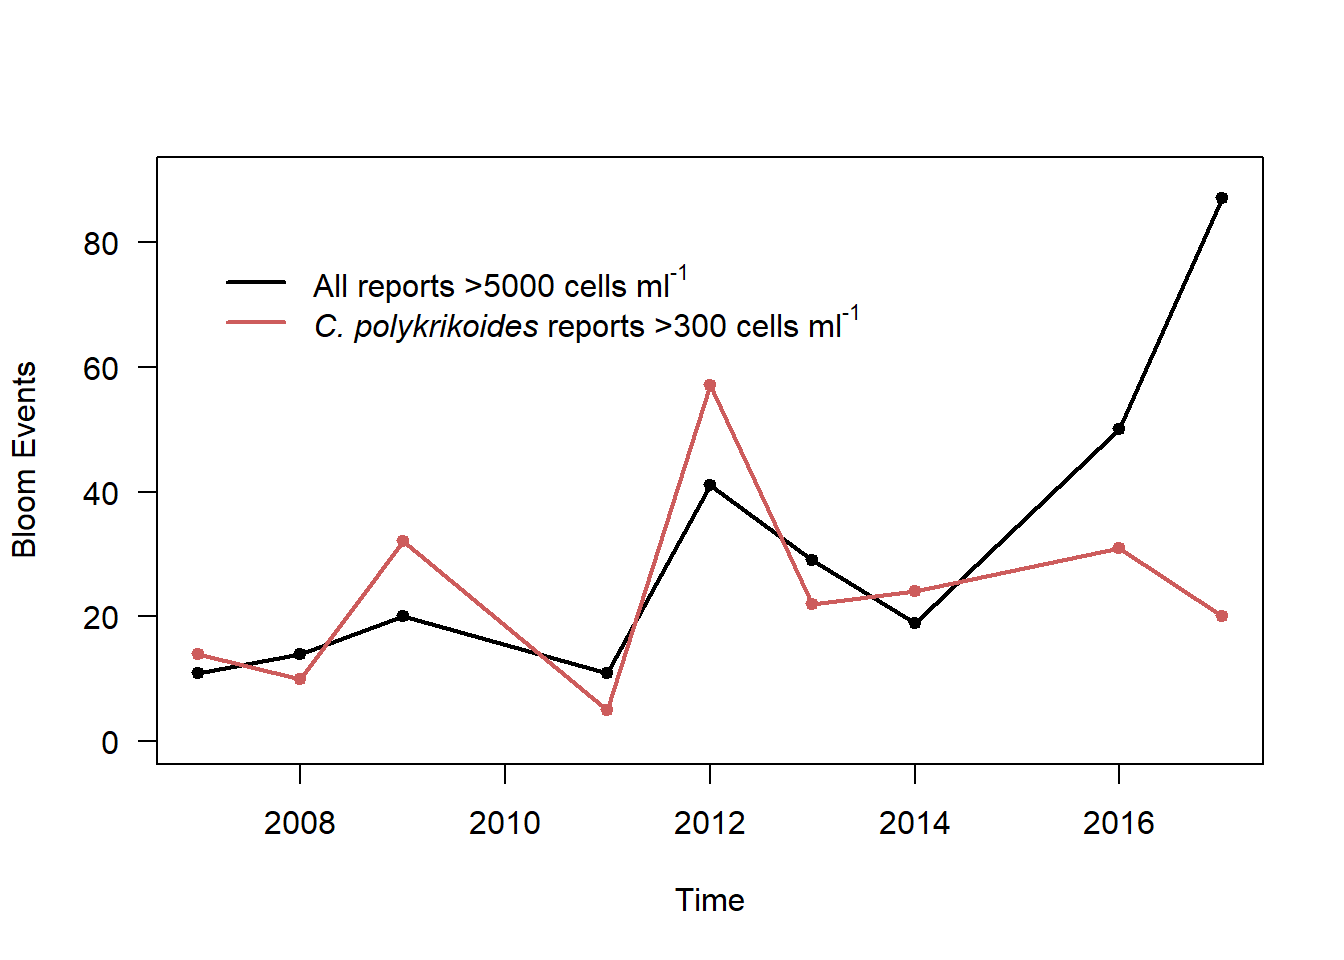
\includegraphics{C:/Users/kimberly.bastille/Desktop/tech-doc/imagesr-extract-1} 

}

\caption{All reported algal blooms >5000 cells ml <sup>-1</sup> (black), and reports of <i>C. polykrikoides</i> blooms >300 cells ml <sup>-1</sup> (red) between 2007-2017.}\label{fig:r-extract}
\end{figure}

\subsection{Data analysis}\label{data-analysis-15}

No data analysis steps took place for this indicator.

\chapter{New England Harmful Algal Bloom
Indicator}\label{new-england-harmful-algal-bloom-indicator}

\textbf{Description}: Regional incidence of shellfish bed closures due
to presence of toxins associated with harmful algae.

\textbf{Found in}: State of the Ecosystem - Gulf of Maine \& Georges
Bank (2018)

\textbf{Indicator Category}: Synthesis of published information

\textbf{Contributor(s)}: Dave Kulis, Donald M Anderson, Sean Hardison

\textbf{Data steward}: Sean Hardison,
\href{mailto:sean.hardison@noaa.gov}{\nolinkurl{sean.hardison@noaa.gov}}

\textbf{Point of contact}: Sean Hardison,
\href{mailto:sean.hardison@noaa.gov}{\nolinkurl{sean.hardison@noaa.gov}}

\textbf{Public availability statement}: Data are publicly available (see
Data Sources below).

\section{Methods}\label{methods-18}

The New England Harmful Algal Bloom (HAB) indicator is a synthesis of
shellfish bed closures related to the presence of HAB-associated toxins
above threshold levels from 2007-2016 (Figure \ref{fig:NE-HAB-image}).
Standard detection methods were used to identify the presence of toxins
associated with Amnesic Shellfish Poisoning (ASP), Paralytic Shellfish
Poisoning (PSP), and Diarrhetic Shellfish Poisoning (DSP) by state and
federal laboratories.

\subsubsection{Paralytic Shellfish
Poisoning}\label{paralytic-shellfish-poisoning}

The most common cause of shellfish bed closures in New England is the
presence of paralytic shellfish toxins (PSTs) produced by the
dinoflagellate \emph{Alexandrium catenella}. All New England states
except Maine relied on the AOAC-approved mouse bioassay method to detect
PSTs in shellfish during the 2007-2016 period reported here
(International \protect\hyperlink{ref-Anonymous2005}{2005}).

In Maine, PST detection methods were updated in May 2014 when the state
adopted the hydrophilic interaction liquid chromatography (HILIC)
UPLC-MS/MS protocol (Boundy et al.
\protect\hyperlink{ref-Boundy2015}{2015}) in concordance with National
Shellfish Sanitation Program (NSSP) requirements. Prior to this, the
primary method used to detect PST in Maine was with the mouse bioassay.

\subsubsection{Amnesic Shellfish
Poisoning}\label{amnesic-shellfish-poisoning}

Amnesic shellfish poisoning (ASP) is caused by the toxin domoic acid
(DA), which is produced by several phytoplankton species belonging to
the genus \emph{Pseudo-nitzchia}. In New England, a UV-HPLC method
(Quilliam, Xie, and Hardstaff
\protect\hyperlink{ref-Quilliam1995}{1995}), which specifies a HPLC-UV
protocol, is used for ASP detection.

\subsubsection{Diarrhetic Shellfish
Poisoning}\label{diarrhetic-shellfish-poisoning}

Diarrhetic Shellfish Poisoning (DSP) is rare in New England waters, but
the presence of the DSP-associated okadaic acid (OA) in mussels was
confirmed in Massachusetts in 2015 (J. Deeds, personal communication,
July 7, 2018). Preliminary testing for OA in Massachusetts utilized the
commercially available Protein Phosphatase Inhibition Assay (PPIA) and
these results are confirmed through LC-MS/MS when necessary (Smienk et
al. \protect\hyperlink{ref-Smienk2012}{2012}; Stutts and Deeds
\protect\hyperlink{ref-Stutts2017}{2017}).

\subsection{Data sources}\label{data-sources-18}

Data used in this indicator were drawn from the 2017 Report on the
ICES-IOC Working Group on Harmful Algal Bloom Dynamics (WGHABD). The
report and data are available
\href{http://www.ices.dk/sites/pub/Publication\%20Reports/Expert\%20Group\%20Report/SSGEPD/2017/01\%20WGHABD\%20-\%20Report\%20of\%20the\%20ICES\%20-\%20IOC\%20Working\%20Group\%20on\%20Harmful\%20Algal\%20Bloom\%20Dynamics.pdf}{here}.

Closure information was collated from information provided by the
following organizations:

\begin{table}

\caption{\label{tab:closuresrc}Shellfish closure information providers.}
\centering
\begin{tabular}[t]{ll}
\toprule
State & Source Organization\\
\midrule
Maine & Maine Department of Marine Resources\\
New Hampshire & New Hampshire Department of Environmental Services\\
Massachusetts & Massachusetts Division of Marine Fisheries\\
Rhode Island & Rhode Island Department of Environmental Management\\
Connecticut & Connecticut Department of Agriculture\\
\bottomrule
\end{tabular}
\end{table}

\subsection{Data extraction}\label{data-extraction-16}

Data were extracted from the original report visually and accuracy
confirmed with report authors.

\subsection{Data analysis}\label{data-analysis-16}

No data analysis steps took place for this indicator.

The script used to develop the figure in the SOE report is below.

\begin{figure}

{\centering 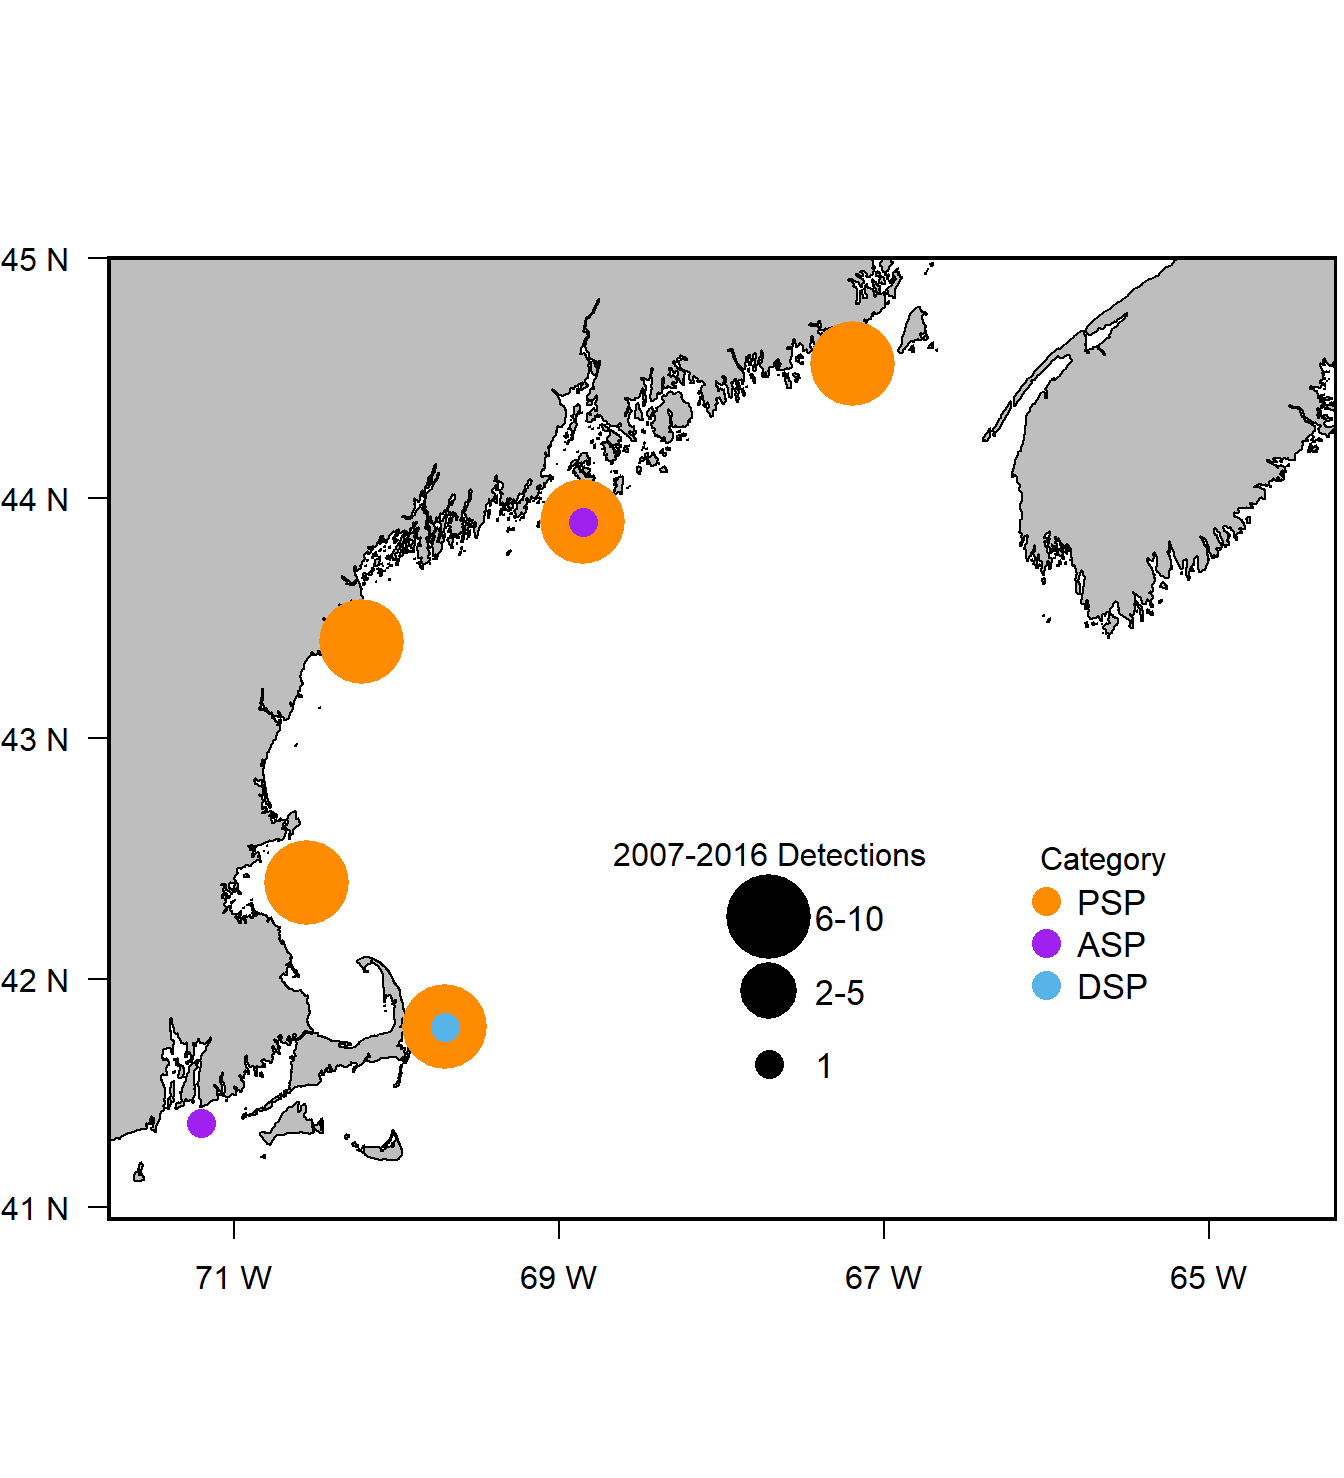
\includegraphics{C:/Users/kimberly.bastille/Desktop/tech-doc/imagesNE-HAB-1} 

}

\caption{Regional HAB related shellfish bed closures in New England between 2007 and 2016.}\label{fig:NE-HAB}
\end{figure}

\chapter{Verified Records of Southern
Kingfish}\label{verified-records-of-southern-kingfish}

\textbf{Description}: Fisheries Observer Data -- Verified Records of
Southern Kingfish

\textbf{Found in}: State of the Ecosystem - Mid-Atlantic (2018)

\textbf{Indicator category}: Database pull

\textbf{Contributor(s)}: Debra Duarte, Loren Kellogg

\textbf{Data steward}: Gina Shield,
\href{mailto:gina.shield@noaa.gov}{\nolinkurl{gina.shield@noaa.gov}}

\textbf{Point of contact}: Gina Shield,
\href{mailto:gina.shield@noaa.gov}{\nolinkurl{gina.shield@noaa.gov}}

\textbf{Public availability statement}: Due to PII concerns data for
this indicator are not publicly available.

\section{Methods}\label{methods-19}

\subsection{Data sources}\label{data-sources-19}

The Fisheries Sampling Branch deploys observers on commercial fisheries
trips from Maine to North Carolina. On observed tows, observers must
fully document all kept and discarded species encountered. Observers
must comply with a Species Verification Program (SVP), which requires
photo or sample submissions of high priority species at least once per
quarter. Photos and samples submitted for verification are identified
independently by at least two reviewers.

The derived data presented in the Mid-Atlantic State of the Ecosystem
report for southern kingfish include records verified by the SVP program
only. The occurrence of southern kingfish in SVP records were chosen for
inclusion in the report due to the recent increases of the species in
SVP observer records since 2010. These data are not a complete list from
the New England Fisheries Observer Program (NEFOP). Southern Kingfish
are less common than Northern Kingfish in observer data and are possibly
misidentified so we have initially included records here only when a
specimen record was submitted to and verified through the SVP (see Data
extraction).

\subsection{Data extraction}\label{data-extraction-17}

SQL query:

\begin{Shaded}
\begin{Highlighting}[]
\CommentTok{/* training trips, 900 trips, incidental takes, most duplicate records (unless different idmethod or idcomment) are not included */}
\CommentTok{/* this is a general script to pull the data on any species from the SVP*/}
\CommentTok{/* specimens submitted as photos and samples included separately */}
\CommentTok{/* nefop_ims.species_verification query that approximates is: select * from nefop_ims.species_verification where SUBJECT_CODE <> '01' and YEAR > '2009' and species = '6617' order by species, year, tripid, haulnum, idmethod but this could includes training trips, duplicates, 900 trips*/}


\KeywordTok{SELECT}\NormalTok{ ss.year }\DataTypeTok{YEAR}\NormalTok{, }\DataTypeTok{MONTH}\NormalTok{, ss.obid }\KeywordTok{as}\NormalTok{ OBSID, ss.tripid TRIPID, NEGEAR, DATELAND, SS.HAUL HAUL, CODE, SPECIES, correct, INCCODE, INCORRECTSPP, idmethod, GIS_LATSBEG, GIS_LONSBEG, GIS_LATSEND, GIS_LONSEND, GIS_LATHBEG, GIS_LONHBEG, GIS_LATHEND, GIS_LONHEND, rr.QTR QTR, rr.link1 link1, rr.link3 LINK3, idcomments}

\KeywordTok{from} 

\NormalTok{(}\KeywordTok{SELECT} \FunctionTok{substr}\NormalTok{(c.tripid, }\DecValTok{1}\NormalTok{,}\DecValTok{3}\NormalTok{) obid, c.tripid, c.year, HAUL, }\FunctionTok{TO_CHAR}\NormalTok{(t.dateland, }\StringTok{'DD-MON-YY'}\NormalTok{) }\KeywordTok{as}\NormalTok{ DATELAND, CODE, SPECIES, correct, INCORRECTSPP }\KeywordTok{as}\NormalTok{ INCCODE, comname }\KeywordTok{as}\NormalTok{ INCORRECTSPP, idmethod, idcomments}

\KeywordTok{FROM} 

\NormalTok{(}\KeywordTok{select}\NormalTok{ id_num, a.tripid, a.year, }\FunctionTok{lpad}\NormalTok{(}\FunctionTok{CAST}\NormalTok{(haulnum }\KeywordTok{as} \DataTypeTok{varchar2}\NormalTok{(}\DecValTok{4}\NormalTok{ byte)),}\DecValTok{4}\NormalTok{,}\StringTok{'0'}\NormalTok{) haul, inc, dateverify, species }\KeywordTok{as}\NormalTok{ CODE, comname }\KeywordTok{as}\NormalTok{ SPECIES, correct, incorrectspp,}
\NormalTok{  idmethod, idcomments, obs_contacted, filelocation}
\KeywordTok{from}\NormalTok{ nefop_ims.species_verification a, obdbs.obspec b}
\KeywordTok{where}\NormalTok{ a.species=b.nespp4) c }
\KeywordTok{left} \KeywordTok{join}\NormalTok{ obdbs.obspec d }
\KeywordTok{on}\NormalTok{ c.incorrectspp=d.nespp4}
\KeywordTok{join}\NormalTok{ OBSCON.OBSCON_TRIPS_FSB t }\KeywordTok{on}\NormalTok{ c.year||c.tripid=t.year||substr(t.LINK1,}\DecValTok{10}\NormalTok{,}\DecValTok{6}\NormalTok{)}
\KeywordTok{where}\NormalTok{ c.YEAR }\KeywordTok{like} \StringTok{'%%'} \KeywordTok{and}\NormalTok{ c.TRIPID }\KeywordTok{like} \StringTok{'%%'} \KeywordTok{and}\NormalTok{ c.inc }\KeywordTok{is} \KeywordTok{null} \KeywordTok{and}\NormalTok{ DATELAND }\KeywordTok{between} \FunctionTok{to_date}\NormalTok{(}\StringTok{'01-JAN-10'}\NormalTok{, }\StringTok{'DD-MON-RR'}\NormalTok{) }\KeywordTok{and} \FunctionTok{to_date}\NormalTok{(}\StringTok{'31-DEC-20'}\NormalTok{,}\StringTok{'DD-MON-RR'}\NormalTok{)}

\KeywordTok{UNION}

\KeywordTok{SELECT} \FunctionTok{substr}\NormalTok{(g.tripid,}\DecValTok{1}\NormalTok{,}\DecValTok{3}\NormalTok{) obid, g.tripid, g.year, HAUL, }\FunctionTok{TO_CHAR}\NormalTok{(s.dateland, }\StringTok{'DD-MON-YY'}\NormalTok{) }\KeywordTok{as}\NormalTok{ DATELAND, CODE, SPECIES, correct, INCORRECTSPP }\KeywordTok{as}\NormalTok{ INCCODE, comname }\KeywordTok{as}\NormalTok{ INCORRECTSPP,}
\NormalTok{  idmethod, idcomments}
\KeywordTok{FROM}\NormalTok{ ((}\KeywordTok{select}\NormalTok{ id_num, e.tripid, e.year, }\FunctionTok{lpad}\NormalTok{(}\FunctionTok{CAST}\NormalTok{(haulnum }\KeywordTok{as} \DataTypeTok{varchar2}\NormalTok{(}\DecValTok{4}\NormalTok{ byte)),}\DecValTok{4}\NormalTok{,}\StringTok{'0'}\NormalTok{) haul, inc, dateverify, species }\KeywordTok{as}\NormalTok{ CODE, comname }\KeywordTok{as}\NormalTok{ SPECIES, correct, incorrectspp,}
\NormalTok{  idmethod, idcomments, obs_contacted, filelocation}
\KeywordTok{from}\NormalTok{ nefop_ims.species_verification e, obdbs.obspec f}
\KeywordTok{where}\NormalTok{ e.species=f.nespp4) g }
\KeywordTok{left} \KeywordTok{join}\NormalTok{ obdbs.obspec h }
\KeywordTok{on}\NormalTok{ g.incorrectspp=h.nespp4}
\KeywordTok{join}\NormalTok{ obdbs.asmtrp_entry s }\KeywordTok{on}\NormalTok{ g.year||g.tripid=s.yearland||s.tripid) }
\KeywordTok{where}\NormalTok{ g.YEAR }\KeywordTok{like} \StringTok{'%%'} \KeywordTok{and}\NormalTok{ g.TRIPID }\KeywordTok{like} \StringTok{'%%'} \KeywordTok{and}\NormalTok{ g.inc }\KeywordTok{is} \KeywordTok{null} \KeywordTok{and}\NormalTok{ DATELAND }\KeywordTok{between} \FunctionTok{to_date}\NormalTok{(}\StringTok{'01-JAN-10'}\NormalTok{, }\StringTok{'DD-MON-RR'}\NormalTok{) }\KeywordTok{and} \FunctionTok{to_date}\NormalTok{(}\StringTok{'31-DEC-20'}\NormalTok{,}\StringTok{'DD-MON-RR'}\NormalTok{)}

\KeywordTok{UNION}

\KeywordTok{SELECT} \FunctionTok{substr}\NormalTok{(r.tripid, }\DecValTok{1}\NormalTok{,}\DecValTok{3}\NormalTok{) obid, r.tripid, r.year, HAUL, }\FunctionTok{TO_CHAR}\NormalTok{(s.dateland, }\StringTok{'DD-MON-YY'}\NormalTok{) }\KeywordTok{as}\NormalTok{ DATELAND, CODE, SPECIES, correct, INCORRECTSPP }\KeywordTok{as}\NormalTok{ INCCODE, comname }\KeywordTok{as}\NormalTok{ INCORRECTSPP,}
\NormalTok{  idmethod, idcomments}
\KeywordTok{FROM}\NormalTok{ ((}\KeywordTok{select}\NormalTok{ id_num, a.tripid, a.year, }\FunctionTok{lpad}\NormalTok{(}\FunctionTok{CAST}\NormalTok{(haulnum }\KeywordTok{as} \DataTypeTok{varchar2}\NormalTok{(}\DecValTok{4}\NormalTok{ byte)),}\DecValTok{4}\NormalTok{,}\StringTok{'0'}\NormalTok{) haul, inc, dateverify, species }\KeywordTok{as}\NormalTok{ CODE, comname }\KeywordTok{as}\NormalTok{ SPECIES, correct, incorrectspp,}
\NormalTok{  idmethod, idcomments, obs_contacted, filelocation}
\KeywordTok{from}\NormalTok{ nefop_ims.species_verification a, obdbs.obspec b}
\KeywordTok{where}\NormalTok{ a.species=b.nespp4) r }
\KeywordTok{left} \KeywordTok{join}\NormalTok{ obdbs.obspec d }
\KeywordTok{on}\NormalTok{ r.incorrectspp=d.nespp4}
\KeywordTok{join}\NormalTok{ OBPRELIM.TRP_BASE s }\KeywordTok{on}\NormalTok{ r.year||r.tripid=s.yearland||S.TRIPID)}
\KeywordTok{where}\NormalTok{ r.YEAR }\KeywordTok{like} \StringTok{'%%'} \KeywordTok{and}\NormalTok{ r.TRIPID }\KeywordTok{like} \StringTok{'%%'} \KeywordTok{and}\NormalTok{ r.inc }\KeywordTok{is} \KeywordTok{null} \KeywordTok{and}\NormalTok{ DATELAND }\KeywordTok{between} \FunctionTok{to_date}\NormalTok{(}\StringTok{'01-JAN-10'}\NormalTok{, }\StringTok{'DD-MON-RR'}\NormalTok{) }\KeywordTok{and} \FunctionTok{to_date}\NormalTok{(}\StringTok{'31-DEC-20'}\NormalTok{,}\StringTok{'DD-MON-RR'}\NormalTok{)) ss}

\KeywordTok{left} \KeywordTok{join}

\NormalTok{(}\CommentTok{/* OBDBS OBHAU */}

\KeywordTok{select}
   \FunctionTok{substr}\NormalTok{(link3,}\DecValTok{1}\NormalTok{,}\DecValTok{15}\NormalTok{)  LINK1 ,}
\NormalTok{   LINK3,   }
   \FunctionTok{substr}\NormalTok{(link3,}\DecValTok{1}\NormalTok{,}\DecValTok{3}\NormalTok{)  PROGRAM ,}
   \FunctionTok{substr}\NormalTok{(link3,}\DecValTok{4}\NormalTok{,}\DecValTok{4}\NormalTok{)   }\DataTypeTok{YEAR}\NormalTok{ ,}
   \FunctionTok{substr}\NormalTok{(link3,}\DecValTok{8}\NormalTok{,}\DecValTok{2}\NormalTok{)   }\DataTypeTok{MONTH}\NormalTok{ ,}
   \FunctionTok{substr}\NormalTok{(link3,}\DecValTok{10}\NormalTok{,}\DecValTok{6}\NormalTok{)  TRIPID ,}
   \FunctionTok{substr}\NormalTok{(link3,}\DecValTok{16}\NormalTok{,}\DecValTok{4}\NormalTok{)  HAULNUM ,}
   \FunctionTok{decode}\NormalTok{(}\FunctionTok{substr}\NormalTok{(link3,}\DecValTok{8}\NormalTok{,}\DecValTok{2}\NormalTok{),}\StringTok{'01'}\NormalTok{,}\DecValTok{1}\NormalTok{,}\StringTok{'02'}\NormalTok{,}\DecValTok{1}\NormalTok{,}\StringTok{'03'}\NormalTok{,}\DecValTok{1}\NormalTok{,}\StringTok{'04'}\NormalTok{,}\DecValTok{2}\NormalTok{,}
           \StringTok{'05'}\NormalTok{,}\DecValTok{2}\NormalTok{,}\StringTok{'06'}\NormalTok{,}\DecValTok{2}\NormalTok{,}\StringTok{'07'}\NormalTok{,}\DecValTok{3}\NormalTok{,}\StringTok{'08'}\NormalTok{,}\DecValTok{3}\NormalTok{,}\StringTok{'09'}\NormalTok{,}\DecValTok{3}\NormalTok{,}\StringTok{'10'}\NormalTok{,}\DecValTok{4}\NormalTok{,}\StringTok{'11'}\NormalTok{,}\DecValTok{4}\NormalTok{,}\StringTok{'12'}\NormalTok{,}\DecValTok{4}\NormalTok{,}\KeywordTok{null}\NormalTok{) QTR,}
\NormalTok{ NEGEAR,}
\NormalTok{ OBSRFLAG,}
\NormalTok{ CATEXIST,}
\KeywordTok{case} \KeywordTok{when}\NormalTok{ yearhbeg }\KeywordTok{is} \KeywordTok{not} \KeywordTok{null} \KeywordTok{and}\NormalTok{ monthhbeg }\KeywordTok{is} \KeywordTok{not} \KeywordTok{null} \KeywordTok{and}\NormalTok{ dayhbeg }\KeywordTok{is} \KeywordTok{not} \KeywordTok{null} \KeywordTok{then}
   \FunctionTok{to_date}\NormalTok{(}\FunctionTok{ltrim}\NormalTok{(}\FunctionTok{rtrim}\NormalTok{(YEARHBEG))||ltrim(}\FunctionTok{rtrim}\NormalTok{(MONTHHBEG))||ltrim(}\FunctionTok{rtrim}\NormalTok{(DAYHBEG))||ltrim(}\FunctionTok{rtrim}\NormalTok{(TIMEHBEG)),}\StringTok{'YYYYMMDDHH24MI'}\NormalTok{)}
\KeywordTok{else} \KeywordTok{null}
\KeywordTok{end}\NormalTok{ datehbeg,}
\KeywordTok{case} \KeywordTok{when}\NormalTok{ yearhend }\KeywordTok{is} \KeywordTok{not} \KeywordTok{null} \KeywordTok{and}\NormalTok{ monthend }\KeywordTok{is} \KeywordTok{not} \KeywordTok{null} \KeywordTok{and}\NormalTok{ dayhend }\KeywordTok{is} \KeywordTok{not} \KeywordTok{null} \KeywordTok{then}
   \FunctionTok{to_date}\NormalTok{(}\FunctionTok{ltrim}\NormalTok{(}\FunctionTok{rtrim}\NormalTok{(YEARHEND))||ltrim(}\FunctionTok{rtrim}\NormalTok{(MONTHEND))||ltrim(}\FunctionTok{rtrim}\NormalTok{(DAYHEND))||ltrim(}\FunctionTok{rtrim}\NormalTok{(TIMEHEND)),}\StringTok{'YYYYMMDDHH24MI'}\NormalTok{)}
\KeywordTok{else} \KeywordTok{null}
\KeywordTok{end}\NormalTok{ datehend,}
\NormalTok{ LATHBEG,}
\NormalTok{ LONHBEG,}
\NormalTok{ LATHEND,}
\NormalTok{ LONHEND,}
 \FunctionTok{cast}\NormalTok{( }\FunctionTok{substr}\NormalTok{(latsbeg,}\DecValTok{1}\NormalTok{,}\DecValTok{2}\NormalTok{) + }\FunctionTok{substr}\NormalTok{(latsbeg,}\DecValTok{3}\NormalTok{,}\DecValTok{2}\NormalTok{) / }\DecValTok{60}\NormalTok{ + }\FunctionTok{substr}\NormalTok{(latsbeg,}\DecValTok{5}\NormalTok{,}\DecValTok{2}\NormalTok{) / }\DecValTok{3600} \KeywordTok{as} \DataTypeTok{number}\NormalTok{(}\DecValTok{8}\NormalTok{,}\DecValTok{6}\NormalTok{)) GIS_LATSBEG ,}
\NormalTok{ -}\DecValTok{1}\NormalTok{ * }\FunctionTok{cast}\NormalTok{(}\FunctionTok{substr}\NormalTok{(lonsbeg,}\DecValTok{1}\NormalTok{,}\DecValTok{2}\NormalTok{) + }\FunctionTok{substr}\NormalTok{(lonsbeg,}\DecValTok{3}\NormalTok{,}\DecValTok{2}\NormalTok{) / }\DecValTok{60}\NormalTok{ + }\FunctionTok{substr}\NormalTok{(lonsbeg,}\DecValTok{5}\NormalTok{,}\DecValTok{2}\NormalTok{) / }\DecValTok{3600} \KeywordTok{as} \DataTypeTok{number}\NormalTok{(}\DecValTok{8}\NormalTok{,}\DecValTok{6}\NormalTok{)) GIS_LONSBEG ,}
  \FunctionTok{cast}\NormalTok{(}\FunctionTok{substr}\NormalTok{(latsend,}\DecValTok{1}\NormalTok{,}\DecValTok{2}\NormalTok{) + }\FunctionTok{substr}\NormalTok{(latsend,}\DecValTok{3}\NormalTok{,}\DecValTok{2}\NormalTok{) / }\DecValTok{60}\NormalTok{ + }\FunctionTok{substr}\NormalTok{(latsend,}\DecValTok{5}\NormalTok{,}\DecValTok{2}\NormalTok{) / }\DecValTok{3600} \KeywordTok{as} \DataTypeTok{number}\NormalTok{(}\DecValTok{8}\NormalTok{,}\DecValTok{6}\NormalTok{)) GIS_LATSEND,}
\NormalTok{  -}\DecValTok{1}\NormalTok{ * }\FunctionTok{cast}\NormalTok{(}\FunctionTok{substr}\NormalTok{(lonsend,}\DecValTok{1}\NormalTok{,}\DecValTok{2}\NormalTok{) + }\FunctionTok{substr}\NormalTok{(lonsend,}\DecValTok{3}\NormalTok{,}\DecValTok{2}\NormalTok{) / }\DecValTok{60}\NormalTok{ + }\FunctionTok{substr}\NormalTok{(lonsend,}\DecValTok{5}\NormalTok{,}\DecValTok{2}\NormalTok{) / }\DecValTok{3600} \KeywordTok{as} \DataTypeTok{number}\NormalTok{(}\DecValTok{8}\NormalTok{,}\DecValTok{6}\NormalTok{)) GIS_LONSEND,}
 \FunctionTok{cast}\NormalTok{(}\FunctionTok{substr}\NormalTok{(lathbeg,}\DecValTok{1}\NormalTok{,}\DecValTok{2}\NormalTok{) + }\FunctionTok{substr}\NormalTok{(lathbeg,}\DecValTok{3}\NormalTok{,}\DecValTok{2}\NormalTok{) / }\DecValTok{60}\NormalTok{ + }\FunctionTok{substr}\NormalTok{(lathbeg,}\DecValTok{5}\NormalTok{,}\DecValTok{2}\NormalTok{) / }\DecValTok{3600} \KeywordTok{as} \DataTypeTok{number}\NormalTok{(}\DecValTok{8}\NormalTok{,}\DecValTok{6}\NormalTok{)) GIS_LATHBEG,}
\NormalTok{ -}\DecValTok{1}\NormalTok{ * }\FunctionTok{cast}\NormalTok{(}\FunctionTok{substr}\NormalTok{(lonhbeg,}\DecValTok{1}\NormalTok{,}\DecValTok{2}\NormalTok{) + }\FunctionTok{substr}\NormalTok{(lonhbeg,}\DecValTok{3}\NormalTok{,}\DecValTok{2}\NormalTok{) / }\DecValTok{60}\NormalTok{ + }\FunctionTok{substr}\NormalTok{(lonhbeg,}\DecValTok{5}\NormalTok{,}\DecValTok{2}\NormalTok{) / }\DecValTok{3600} \KeywordTok{as} \DataTypeTok{number}\NormalTok{(}\DecValTok{8}\NormalTok{,}\DecValTok{6}\NormalTok{)) GIS_LONHBEG,}
 \FunctionTok{cast}\NormalTok{(}\FunctionTok{substr}\NormalTok{(lathend,}\DecValTok{1}\NormalTok{,}\DecValTok{2}\NormalTok{) + }\FunctionTok{substr}\NormalTok{(lathend,}\DecValTok{3}\NormalTok{,}\DecValTok{2}\NormalTok{) / }\DecValTok{60}\NormalTok{ + }\FunctionTok{substr}\NormalTok{(lathend,}\DecValTok{5}\NormalTok{,}\DecValTok{2}\NormalTok{) / }\DecValTok{3600} \KeywordTok{as} \DataTypeTok{number}\NormalTok{(}\DecValTok{8}\NormalTok{,}\DecValTok{6}\NormalTok{)) GIS_LATHEND,}
\NormalTok{ -}\DecValTok{1}\NormalTok{ * }\FunctionTok{cast}\NormalTok{(}\FunctionTok{substr}\NormalTok{(lonhend,}\DecValTok{1}\NormalTok{,}\DecValTok{2}\NormalTok{) + }\FunctionTok{substr}\NormalTok{(lonhend,}\DecValTok{3}\NormalTok{,}\DecValTok{2}\NormalTok{) / }\DecValTok{60}\NormalTok{ + }\FunctionTok{substr}\NormalTok{(lonhend,}\DecValTok{5}\NormalTok{,}\DecValTok{2}\NormalTok{) / }\DecValTok{3600} \KeywordTok{as} \DataTypeTok{number}\NormalTok{(}\DecValTok{8}\NormalTok{,}\DecValTok{6}\NormalTok{)) GIS_LONHEND,}
\NormalTok{ AREA,}
\NormalTok{ HAUCOMMENTS}
   \KeywordTok{from}\NormalTok{ obdbs.obhau_base}

    
\KeywordTok{UNION}
    \KeywordTok{select}
   \FunctionTok{substr}\NormalTok{(link3,}\DecValTok{1}\NormalTok{,}\DecValTok{15}\NormalTok{)  LINK1 ,}
\NormalTok{   LINK3,}
   \FunctionTok{substr}\NormalTok{(link3,}\DecValTok{1}\NormalTok{,}\DecValTok{3}\NormalTok{)  PROGRAM ,}
   \FunctionTok{substr}\NormalTok{(link3,}\DecValTok{4}\NormalTok{,}\DecValTok{4}\NormalTok{)   }\DataTypeTok{YEAR}\NormalTok{ ,}
   \FunctionTok{substr}\NormalTok{(link3,}\DecValTok{8}\NormalTok{,}\DecValTok{2}\NormalTok{)   }\DataTypeTok{MONTH}\NormalTok{ ,}
   \FunctionTok{substr}\NormalTok{(link3,}\DecValTok{10}\NormalTok{,}\DecValTok{6}\NormalTok{)  TRIPID ,}
   \FunctionTok{substr}\NormalTok{(link3,}\DecValTok{16}\NormalTok{,}\DecValTok{4}\NormalTok{)  HAULNUM ,}
   \FunctionTok{decode}\NormalTok{(}\FunctionTok{substr}\NormalTok{(link3,}\DecValTok{8}\NormalTok{,}\DecValTok{2}\NormalTok{),}\StringTok{'01'}\NormalTok{,}\DecValTok{1}\NormalTok{,}\StringTok{'02'}\NormalTok{,}\DecValTok{1}\NormalTok{,}\StringTok{'03'}\NormalTok{,}\DecValTok{1}\NormalTok{,}\StringTok{'04'}\NormalTok{,}\DecValTok{2}\NormalTok{,}
           \StringTok{'05'}\NormalTok{,}\DecValTok{2}\NormalTok{,}\StringTok{'06'}\NormalTok{,}\DecValTok{2}\NormalTok{,}\StringTok{'07'}\NormalTok{,}\DecValTok{3}\NormalTok{,}\StringTok{'08'}\NormalTok{,}\DecValTok{3}\NormalTok{,}\StringTok{'09'}\NormalTok{,}\DecValTok{3}\NormalTok{,}\StringTok{'10'}\NormalTok{,}\DecValTok{4}\NormalTok{,}\StringTok{'11'}\NormalTok{,}\DecValTok{4}\NormalTok{,}\StringTok{'12'}\NormalTok{,}\DecValTok{4}\NormalTok{,}\KeywordTok{null}\NormalTok{) QTR,}

\NormalTok{ NEGEAR,}
\NormalTok{ OBSRFLAG,}
\NormalTok{ CATEXIST,}
\KeywordTok{case} \KeywordTok{when}\NormalTok{ yearhbeg }\KeywordTok{is} \KeywordTok{not} \KeywordTok{null} \KeywordTok{and}\NormalTok{ monthhbeg }\KeywordTok{is} \KeywordTok{not} \KeywordTok{null} \KeywordTok{and}\NormalTok{ dayhbeg }\KeywordTok{is} \KeywordTok{not} \KeywordTok{null} \KeywordTok{then}
   \FunctionTok{to_date}\NormalTok{(}\FunctionTok{ltrim}\NormalTok{(}\FunctionTok{rtrim}\NormalTok{(YEARHBEG))||ltrim(}\FunctionTok{rtrim}\NormalTok{(MONTHHBEG))||ltrim(}\FunctionTok{rtrim}\NormalTok{(DAYHBEG))||ltrim(}\FunctionTok{rtrim}\NormalTok{(TIMEHBEG)),}\StringTok{'YYYYMMDDHH24MI'}\NormalTok{)}
\KeywordTok{else} \KeywordTok{null}
\KeywordTok{end}\NormalTok{ datehbeg,}
\KeywordTok{case} \KeywordTok{when}\NormalTok{ yearhend }\KeywordTok{is} \KeywordTok{not} \KeywordTok{null} \KeywordTok{and}\NormalTok{ monthend }\KeywordTok{is} \KeywordTok{not} \KeywordTok{null} \KeywordTok{and}\NormalTok{ dayhend }\KeywordTok{is} \KeywordTok{not} \KeywordTok{null} \KeywordTok{then}
   \FunctionTok{to_date}\NormalTok{(}\FunctionTok{ltrim}\NormalTok{(}\FunctionTok{rtrim}\NormalTok{(YEARHEND))||ltrim(}\FunctionTok{rtrim}\NormalTok{(MONTHEND))||ltrim(}\FunctionTok{rtrim}\NormalTok{(DAYHEND))||ltrim(}\FunctionTok{rtrim}\NormalTok{(TIMEHEND)),}\StringTok{'YYYYMMDDHH24MI'}\NormalTok{)}
\KeywordTok{else} \KeywordTok{null}
\KeywordTok{end}\NormalTok{ datehend,}
\NormalTok{ LATHBEG,}
\NormalTok{ LONHBEG, }
\NormalTok{ LATHEND,}
\NormalTok{ LONHEND,}
 \FunctionTok{cast}\NormalTok{( }\FunctionTok{substr}\NormalTok{(latsbeg,}\DecValTok{1}\NormalTok{,}\DecValTok{2}\NormalTok{) + }\FunctionTok{substr}\NormalTok{(latsbeg,}\DecValTok{3}\NormalTok{,}\DecValTok{2}\NormalTok{) / }\DecValTok{60}\NormalTok{ + }\FunctionTok{substr}\NormalTok{(latsbeg,}\DecValTok{5}\NormalTok{,}\DecValTok{2}\NormalTok{) / }\DecValTok{3600} \KeywordTok{as} \DataTypeTok{number}\NormalTok{(}\DecValTok{8}\NormalTok{,}\DecValTok{6}\NormalTok{)) GIS_LATSBEG ,}
\NormalTok{ -}\DecValTok{1}\NormalTok{ * }\FunctionTok{cast}\NormalTok{(}\FunctionTok{substr}\NormalTok{(lonsbeg,}\DecValTok{1}\NormalTok{,}\DecValTok{2}\NormalTok{) + }\FunctionTok{substr}\NormalTok{(lonsbeg,}\DecValTok{3}\NormalTok{,}\DecValTok{2}\NormalTok{) / }\DecValTok{60}\NormalTok{ + }\FunctionTok{substr}\NormalTok{(lonsbeg,}\DecValTok{5}\NormalTok{,}\DecValTok{2}\NormalTok{) / }\DecValTok{3600} \KeywordTok{as} \DataTypeTok{number}\NormalTok{(}\DecValTok{8}\NormalTok{,}\DecValTok{6}\NormalTok{)) GIS_LONSBEG ,}
 \FunctionTok{cast}\NormalTok{(}\FunctionTok{substr}\NormalTok{(latsend,}\DecValTok{1}\NormalTok{,}\DecValTok{2}\NormalTok{) + }\FunctionTok{substr}\NormalTok{(latsend,}\DecValTok{3}\NormalTok{,}\DecValTok{2}\NormalTok{) / }\DecValTok{60}\NormalTok{ + }\FunctionTok{substr}\NormalTok{(latsend,}\DecValTok{5}\NormalTok{,}\DecValTok{2}\NormalTok{) / }\DecValTok{3600} \KeywordTok{as} \DataTypeTok{number}\NormalTok{(}\DecValTok{8}\NormalTok{,}\DecValTok{6}\NormalTok{)) GIS_LATSEND,}
\NormalTok{ -}\DecValTok{1}\NormalTok{ * }\FunctionTok{cast}\NormalTok{(}\FunctionTok{substr}\NormalTok{(lonsend,}\DecValTok{1}\NormalTok{,}\DecValTok{2}\NormalTok{) + }\FunctionTok{substr}\NormalTok{(lonsend,}\DecValTok{3}\NormalTok{,}\DecValTok{2}\NormalTok{) / }\DecValTok{60}\NormalTok{ + }\FunctionTok{substr}\NormalTok{(lonsend,}\DecValTok{5}\NormalTok{,}\DecValTok{2}\NormalTok{) / }\DecValTok{3600} \KeywordTok{as} \DataTypeTok{number}\NormalTok{(}\DecValTok{8}\NormalTok{,}\DecValTok{6}\NormalTok{)) GIS_LONSEND,}
 \FunctionTok{cast}\NormalTok{(}\FunctionTok{substr}\NormalTok{(lathbeg,}\DecValTok{1}\NormalTok{,}\DecValTok{2}\NormalTok{) + }\FunctionTok{substr}\NormalTok{(lathbeg,}\DecValTok{3}\NormalTok{,}\DecValTok{2}\NormalTok{) / }\DecValTok{60}\NormalTok{ + }\FunctionTok{substr}\NormalTok{(lathbeg,}\DecValTok{5}\NormalTok{,}\DecValTok{2}\NormalTok{) / }\DecValTok{3600} \KeywordTok{as} \DataTypeTok{number}\NormalTok{(}\DecValTok{8}\NormalTok{,}\DecValTok{6}\NormalTok{)) GIS_LATHBEG,}
\NormalTok{ -}\DecValTok{1}\NormalTok{ * }\FunctionTok{cast}\NormalTok{(}\FunctionTok{substr}\NormalTok{(lonhbeg,}\DecValTok{1}\NormalTok{,}\DecValTok{2}\NormalTok{) + }\FunctionTok{substr}\NormalTok{(lonhbeg,}\DecValTok{3}\NormalTok{,}\DecValTok{2}\NormalTok{) / }\DecValTok{60}\NormalTok{ + }\FunctionTok{substr}\NormalTok{(lonhbeg,}\DecValTok{5}\NormalTok{,}\DecValTok{2}\NormalTok{) / }\DecValTok{3600} \KeywordTok{as} \DataTypeTok{number}\NormalTok{(}\DecValTok{8}\NormalTok{,}\DecValTok{6}\NormalTok{)) GIS_LONHBEG,}
 \FunctionTok{cast}\NormalTok{(}\FunctionTok{substr}\NormalTok{(lathend,}\DecValTok{1}\NormalTok{,}\DecValTok{2}\NormalTok{) + }\FunctionTok{substr}\NormalTok{(lathend,}\DecValTok{3}\NormalTok{,}\DecValTok{2}\NormalTok{) / }\DecValTok{60}\NormalTok{ + }\FunctionTok{substr}\NormalTok{(lathend,}\DecValTok{5}\NormalTok{,}\DecValTok{2}\NormalTok{) / }\DecValTok{3600} \KeywordTok{as} \DataTypeTok{number}\NormalTok{(}\DecValTok{8}\NormalTok{,}\DecValTok{6}\NormalTok{)) GIS_LATHEND,}
\NormalTok{ -}\DecValTok{1}\NormalTok{ * }\FunctionTok{cast}\NormalTok{(}\FunctionTok{substr}\NormalTok{(lonhend,}\DecValTok{1}\NormalTok{,}\DecValTok{2}\NormalTok{) + }\FunctionTok{substr}\NormalTok{(lonhend,}\DecValTok{3}\NormalTok{,}\DecValTok{2}\NormalTok{) / }\DecValTok{60}\NormalTok{ + }\FunctionTok{substr}\NormalTok{(lonhend,}\DecValTok{5}\NormalTok{,}\DecValTok{2}\NormalTok{) / }\DecValTok{3600} \KeywordTok{as} \DataTypeTok{number}\NormalTok{(}\DecValTok{8}\NormalTok{,}\DecValTok{6}\NormalTok{)) GIS_LONHEND,}
\NormalTok{ AREA,}
\NormalTok{ HAUCOMMENTS}
   \KeywordTok{from}\NormalTok{ obv10.obhau_base}


\KeywordTok{UNION}

\CommentTok{/*  ASM HAU  */}

\KeywordTok{select}
   \FunctionTok{substr}\NormalTok{(link3,}\DecValTok{1}\NormalTok{,}\DecValTok{15}\NormalTok{)  LINK1 ,}
\NormalTok{   LINK3,}
   \FunctionTok{substr}\NormalTok{(link3,}\DecValTok{1}\NormalTok{,}\DecValTok{3}\NormalTok{)  PROGRAM ,}
   \FunctionTok{substr}\NormalTok{(link3,}\DecValTok{4}\NormalTok{,}\DecValTok{4}\NormalTok{)   }\DataTypeTok{YEAR}\NormalTok{ ,}
   \FunctionTok{substr}\NormalTok{(link3,}\DecValTok{8}\NormalTok{,}\DecValTok{2}\NormalTok{)   }\DataTypeTok{MONTH}\NormalTok{ ,}
   \FunctionTok{substr}\NormalTok{(link3,}\DecValTok{10}\NormalTok{,}\DecValTok{6}\NormalTok{)  TRIPID ,}
   \FunctionTok{substr}\NormalTok{(link3,}\DecValTok{16}\NormalTok{,}\DecValTok{4}\NormalTok{)  HAULNUM ,}

   \FunctionTok{decode}\NormalTok{(}\FunctionTok{substr}\NormalTok{(link3,}\DecValTok{8}\NormalTok{,}\DecValTok{2}\NormalTok{),}\StringTok{'01'}\NormalTok{,}\DecValTok{1}\NormalTok{,}\StringTok{'02'}\NormalTok{,}\DecValTok{1}\NormalTok{,}\StringTok{'03'}\NormalTok{,}\DecValTok{1}\NormalTok{,}\StringTok{'04'}\NormalTok{,}\DecValTok{2}\NormalTok{,}
           \StringTok{'05'}\NormalTok{,}\DecValTok{2}\NormalTok{,}\StringTok{'06'}\NormalTok{,}\DecValTok{2}\NormalTok{,}\StringTok{'07'}\NormalTok{,}\DecValTok{3}\NormalTok{,}\StringTok{'08'}\NormalTok{,}\DecValTok{3}\NormalTok{,}\StringTok{'09'}\NormalTok{,}\DecValTok{3}\NormalTok{,}\StringTok{'10'}\NormalTok{,}\DecValTok{4}\NormalTok{,}\StringTok{'11'}\NormalTok{,}\DecValTok{4}\NormalTok{,}\StringTok{'12'}\NormalTok{,}\DecValTok{4}\NormalTok{,}\KeywordTok{null}\NormalTok{) QTR,}
\NormalTok{ NEGEAR,}
\NormalTok{ OBSRFLAG,}
 \FunctionTok{cast}\NormalTok{(}\KeywordTok{null} \KeywordTok{as} \DataTypeTok{varchar2}\NormalTok{(}\DecValTok{1}\NormalTok{)) CATEXIST,}
   \FunctionTok{to_date}\NormalTok{(}\FunctionTok{ltrim}\NormalTok{(}\FunctionTok{rtrim}\NormalTok{(YEARHBEG))||ltrim(}\FunctionTok{rtrim}\NormalTok{(MONTHHBEG))||ltrim(}\FunctionTok{rtrim}\NormalTok{(DAYHBEG))||ltrim(}\FunctionTok{rtrim}\NormalTok{(TIMEHBEG)),}\StringTok{'YYYYMMDDHH24MI'}\NormalTok{)datehbeg, }
   \FunctionTok{to_date}\NormalTok{(}\FunctionTok{ltrim}\NormalTok{(}\FunctionTok{rtrim}\NormalTok{(YEARHEND))||ltrim(}\FunctionTok{rtrim}\NormalTok{(MONTHEND))||ltrim(}\FunctionTok{rtrim}\NormalTok{(DAYHEND))||ltrim(}\FunctionTok{rtrim}\NormalTok{(TIMEHEND)),}\StringTok{'YYYYMMDDHH24MI'}\NormalTok{)datehend, }
\NormalTok{ LATHBEG,}
\NormalTok{ LONHBEG,}
\NormalTok{ LATHEND,}
\NormalTok{ LONHEND,}
 \FunctionTok{cast}\NormalTok{(}\KeywordTok{null} \KeywordTok{as} \DataTypeTok{number}\NormalTok{(}\DecValTok{8}\NormalTok{,}\DecValTok{6}\NormalTok{)) GIS_LATSBEG ,}
 \FunctionTok{cast}\NormalTok{(}\KeywordTok{null} \KeywordTok{as} \DataTypeTok{number}\NormalTok{) GIS_LONSBEG ,}
 \FunctionTok{cast}\NormalTok{(}\KeywordTok{null} \KeywordTok{as} \DataTypeTok{number}\NormalTok{(}\DecValTok{8}\NormalTok{,}\DecValTok{6}\NormalTok{)) GIS_LATSEND,}
 \FunctionTok{cast}\NormalTok{(}\KeywordTok{null} \KeywordTok{as} \DataTypeTok{number}\NormalTok{) GIS_LONSEND,}
 \FunctionTok{cast}\NormalTok{(}\FunctionTok{substr}\NormalTok{(lathbeg,}\DecValTok{1}\NormalTok{,}\DecValTok{2}\NormalTok{) + }\FunctionTok{substr}\NormalTok{(lathbeg,}\DecValTok{3}\NormalTok{,}\DecValTok{2}\NormalTok{) / }\DecValTok{60}\NormalTok{ + }\FunctionTok{substr}\NormalTok{(lathbeg,}\DecValTok{5}\NormalTok{,}\DecValTok{2}\NormalTok{) / }\DecValTok{3600} \KeywordTok{as} \DataTypeTok{number}\NormalTok{(}\DecValTok{8}\NormalTok{,}\DecValTok{6}\NormalTok{)) GIS_LATHBEG,}
\NormalTok{ -}\DecValTok{1}\NormalTok{ * }\FunctionTok{cast}\NormalTok{(}\FunctionTok{substr}\NormalTok{(lonhbeg,}\DecValTok{1}\NormalTok{,}\DecValTok{2}\NormalTok{) + }\FunctionTok{substr}\NormalTok{(lonhbeg,}\DecValTok{3}\NormalTok{,}\DecValTok{2}\NormalTok{) / }\DecValTok{60}\NormalTok{ + }\FunctionTok{substr}\NormalTok{(lonhbeg,}\DecValTok{5}\NormalTok{,}\DecValTok{2}\NormalTok{) / }\DecValTok{3600} \KeywordTok{as} \DataTypeTok{number}\NormalTok{(}\DecValTok{8}\NormalTok{,}\DecValTok{6}\NormalTok{)) GIS_LONHBEG,}
 \FunctionTok{cast}\NormalTok{(}\FunctionTok{substr}\NormalTok{(lathend,}\DecValTok{1}\NormalTok{,}\DecValTok{2}\NormalTok{) + }\FunctionTok{substr}\NormalTok{(lathend,}\DecValTok{3}\NormalTok{,}\DecValTok{2}\NormalTok{) / }\DecValTok{60}\NormalTok{ + }\FunctionTok{substr}\NormalTok{(lathend,}\DecValTok{5}\NormalTok{,}\DecValTok{2}\NormalTok{) / }\DecValTok{3600} \KeywordTok{as} \DataTypeTok{number}\NormalTok{(}\DecValTok{8}\NormalTok{,}\DecValTok{6}\NormalTok{)) GIS_LATHEND,}
\NormalTok{ -}\DecValTok{1}\NormalTok{ * }\FunctionTok{cast}\NormalTok{(}\FunctionTok{substr}\NormalTok{(lonhend,}\DecValTok{1}\NormalTok{,}\DecValTok{2}\NormalTok{) + }\FunctionTok{substr}\NormalTok{(lonhend,}\DecValTok{3}\NormalTok{,}\DecValTok{2}\NormalTok{) / }\DecValTok{60}\NormalTok{ + }\FunctionTok{substr}\NormalTok{(lonhend,}\DecValTok{5}\NormalTok{,}\DecValTok{2}\NormalTok{) / }\DecValTok{3600} \KeywordTok{as} \DataTypeTok{number}\NormalTok{(}\DecValTok{8}\NormalTok{,}\DecValTok{6}\NormalTok{)) GIS_LONHEND,}
\NormalTok{ AREA,}
\NormalTok{ HAUCOMMENTS}
 
   \KeywordTok{from}\NormalTok{ asmhau_prelim p}
 \KeywordTok{left} \KeywordTok{outer} \KeywordTok{join}\NormalTok{ obtriptrack t }
      \KeywordTok{on} \FunctionTok{substr}\NormalTok{(p.link3,}\DecValTok{1}\NormalTok{,}\DecValTok{15}\NormalTok{) = t.link1 }
  \KeywordTok{where}\NormalTok{ (}\FunctionTok{substr}\NormalTok{(link3,}\DecValTok{4}\NormalTok{,}\DecValTok{6}\NormalTok{) }\KeywordTok{between} \StringTok{'201005'} \KeywordTok{and} \StringTok{'201012'} \KeywordTok{and} \FunctionTok{substr}\NormalTok{(link3,}\DecValTok{1}\NormalTok{,}\DecValTok{3}\NormalTok{) }\KeywordTok{between} \StringTok{'230'} \KeywordTok{and} \StringTok{'234'}\NormalTok{)}
     \KeywordTok{or}\NormalTok{ (}\FunctionTok{substr}\NormalTok{(link3,}\DecValTok{4}\NormalTok{,}\DecValTok{6}\NormalTok{) > }\StringTok{'201012'} \KeywordTok{and} \FunctionTok{substr}\NormalTok{(link3,}\DecValTok{1}\NormalTok{,}\DecValTok{3}\NormalTok{) <> }\StringTok{'900'}\NormalTok{)}
    \KeywordTok{and} \FunctionTok{substr}\NormalTok{(link3,}\DecValTok{1}\NormalTok{,}\DecValTok{15}\NormalTok{) }\KeywordTok{not} \KeywordTok{in}\NormalTok{ (}\KeywordTok{select}\NormalTok{ link1 }\KeywordTok{from}\NormalTok{ obv10.obtrp_base) ) rr}
    
\KeywordTok{on}\NormalTok{ ss.YEAR||ss.TRIPID||ss.HAUL = rr.YEAR||rr.TRIPID||ltrim(rr.HAULNUM)}

\KeywordTok{where}\NormalTok{ ss.OBID }\KeywordTok{like} \StringTok{'%%'} \KeywordTok{and}\NormalTok{ ss.TRIPID }\KeywordTok{like} \StringTok{'%%'} \KeywordTok{and}\NormalTok{ (CODE }\KeywordTok{like} \StringTok{'%6617%'}\NormalTok{) }\KeywordTok{and}\NormalTok{ HAUL }\KeywordTok{like} \StringTok{'%%'} \KeywordTok{and}\NormalTok{ SPECIES }\KeywordTok{like} \StringTok{'%%'} \KeywordTok{and}\NormalTok{ IDCOMMENTS }\KeywordTok{like} \StringTok{'%%'} 

\KeywordTok{ORDER} \KeywordTok{BY}\NormalTok{ SPECIES, }\DataTypeTok{YEAR}\NormalTok{, TRIPID, HAUL}
\NormalTok{;}
\end{Highlighting}
\end{Shaded}

\subsection{Data analysis}\label{data-analysis-17}

Time series were summed by year and plotted, and mapped data for
individual records were plotted according to the location where gear was
hauled. As coordinate data were not always available for each record,
the map does not include all occurrences of southern kingfish, but was
included for spatial context.

R code use to aggregate data:

\begin{Shaded}
\begin{Highlighting}[]
\KeywordTok{library}\NormalTok{(dplyr)}

\NormalTok{total_by_year<-}\StringTok{ }\NormalTok{source }\OperatorTok
\StringTok{  }\KeywordTok{filter}\NormalTok{(SPECIES }\OperatorTok{==}\StringTok{ "KINGFISH, SOUTHERN"}\NormalTok{) }\OperatorTok\StringTok{ }\CommentTok{#Filter species}
\StringTok{  }\KeywordTok{group_by}\NormalTok{(YEAR) }\OperatorTok
\StringTok{  }\NormalTok{dplyr}\OperatorTok{::}\KeywordTok{summarise}\NormalTok{(}\DataTypeTok{n =} \KeywordTok{n}\NormalTok{()) }\CommentTok{#Sum observations per year}
\end{Highlighting}
\end{Shaded}

\subsection{Plotting}\label{plotting-12}

\begin{Shaded}
\begin{Highlighting}[]
\CommentTok{#For map and plot. Latitude and longitude data for this figure are not publicly available. }
\NormalTok{sk.dat <-}\StringTok{ }\NormalTok{SOE.data[}\KeywordTok{grepl}\NormalTok{(}\StringTok{"Lat"}\NormalTok{,SOE.data}\OperatorTok{$}\NormalTok{Units) }\OperatorTok{&}
\StringTok{                          }\KeywordTok{grepl}\NormalTok{(}\StringTok{"Southern Kingfish"}\NormalTok{,SOE.data}\OperatorTok{$}\NormalTok{Var),]}
\NormalTok{lon <-}\StringTok{ }\NormalTok{sk.dat[}\KeywordTok{as.numeric}\NormalTok{(sk.dat}\OperatorTok{$}\NormalTok{Value) }\OperatorTok{<}\StringTok{ }\DecValTok{0}\NormalTok{,]}\OperatorTok{$}\NormalTok{Value}
\NormalTok{lat <-}\StringTok{ }\NormalTok{sk.dat[}\KeywordTok{as.numeric}\NormalTok{(sk.dat}\OperatorTok{$}\NormalTok{Value) }\OperatorTok{>}\StringTok{ }\DecValTok{0}\NormalTok{,]}\OperatorTok{$}\NormalTok{Value}

\CommentTok{#create data.frame}
\NormalTok{df <-}\StringTok{ }\KeywordTok{data.frame}\NormalTok{(}\DataTypeTok{year =}\NormalTok{ sk.dat}\OperatorTok{$}\NormalTok{Time,}
                 \DataTypeTok{lon =}\NormalTok{ lon,}
                 \DataTypeTok{lat =}\NormalTok{ lat)}

\CommentTok{#set color palette}
\NormalTok{colors1 <-}\StringTok{ }\KeywordTok{adjustcolor}\NormalTok{(}\KeywordTok{matlab.like2}\NormalTok{(}\DecValTok{8}\NormalTok{),.}\DecValTok{5}\NormalTok{)}
\NormalTok{colors2 <-}\StringTok{ }\KeywordTok{adjustcolor}\NormalTok{(}\KeywordTok{matlab.like2}\NormalTok{(}\DecValTok{8}\NormalTok{),.}\DecValTok{5}\NormalTok{)}
\NormalTok{colors3 <-}\StringTok{ }\KeywordTok{adjustcolor}\NormalTok{(}\KeywordTok{matlab.like2}\NormalTok{(}\DecValTok{8}\NormalTok{),.}\DecValTok{5}\NormalTok{)}
\NormalTok{colors4 <-}\StringTok{ }\KeywordTok{adjustcolor}\NormalTok{(}\KeywordTok{matlab.like2}\NormalTok{(}\DecValTok{8}\NormalTok{),}\DecValTok{1}\NormalTok{)}
\NormalTok{colors <-}\StringTok{ }\KeywordTok{c}\NormalTok{(colors1[}\DecValTok{1}\OperatorTok{:}\DecValTok{2}\NormalTok{], colors2[}\DecValTok{3}\OperatorTok{:}\DecValTok{4}\NormalTok{], colors3[}\DecValTok{5}\OperatorTok{:}\DecValTok{6}\NormalTok{],colors4[}\DecValTok{7}\OperatorTok{:}\DecValTok{8}\NormalTok{])}

\CommentTok{#map values to colors}
\NormalTok{df <-}\StringTok{ }\NormalTok{df }\OperatorTok\StringTok{ }\KeywordTok{arrange}\NormalTok{(year) }\OperatorTok
\StringTok{  }\KeywordTok{mutate}\NormalTok{(}\DataTypeTok{colors =}\NormalTok{ plyr}\OperatorTok{::}\KeywordTok{mapvalues}\NormalTok{(year, }\DataTypeTok{from =} \KeywordTok{c}\NormalTok{(}\StringTok{"2010"}\NormalTok{,}\StringTok{"2011"}\NormalTok{,}\StringTok{"2012"}\NormalTok{,}\StringTok{"2013"}\NormalTok{,}
                                                 \StringTok{"2014"}\NormalTok{,}\StringTok{"2015"}\NormalTok{,}\StringTok{"2016"}\NormalTok{,}\StringTok{"2017"}\NormalTok{),}
                                                               \DataTypeTok{to =} \KeywordTok{c}\NormalTok{(colors)))}
\NormalTok{colors <-}\StringTok{ }\NormalTok{df}\OperatorTok{$}\NormalTok{colors}

\CommentTok{#projection}
\NormalTok{map.crs <-}\StringTok{ }\KeywordTok{CRS}\NormalTok{(}\StringTok{"+proj=longlat +lat_1=35 +lat_2=45 +lat_0=40 +lon_0=-77 +x_0=0}
\StringTok{               +y_0=0 +datum=NAD83 +no_defs +ellps=GRS80 +towgs84=0,0,0"}\NormalTok{)}

\CommentTok{#data.frame to sp object}
\KeywordTok{coordinates}\NormalTok{(df) <-}\StringTok{ }\ErrorTok{~}\NormalTok{lon}\OperatorTok{+}\NormalTok{lat}
\NormalTok{df}\OperatorTok{@}\NormalTok{proj4string <-}\StringTok{ }\NormalTok{map.crs}
\NormalTok{df <-}\StringTok{ }\KeywordTok{spTransform}\NormalTok{(df, map.crs)}

\CommentTok{#plot}
\KeywordTok{par}\NormalTok{(}\DataTypeTok{fig =} \KeywordTok{c}\NormalTok{(}\DecValTok{0}\NormalTok{,}\DecValTok{1}\NormalTok{,}\DecValTok{0}\NormalTok{,}\DecValTok{1}\NormalTok{))}
\KeywordTok{plot}\NormalTok{(coast, }\DataTypeTok{xlim =} \KeywordTok{c}\NormalTok{(}\OperatorTok{-}\DecValTok{76}\NormalTok{,}\OperatorTok{-}\DecValTok{73}\NormalTok{), }\DataTypeTok{ylim =} \KeywordTok{c}\NormalTok{(}\DecValTok{35}\NormalTok{,}\FloatTok{40.5}\NormalTok{),}\DataTypeTok{col =} \StringTok{"grey"}\NormalTok{)}
\KeywordTok{plot}\NormalTok{(df, }\DataTypeTok{pch =} \DecValTok{16}\NormalTok{, }\DataTypeTok{col =}\NormalTok{ colors, }\DataTypeTok{add =}\NormalTok{ T, }\DataTypeTok{cex =} \FloatTok{2.5}\NormalTok{)}


\NormalTok{occur <-}\StringTok{ }\NormalTok{SOE.data[SOE.data}\OperatorTok{$}\NormalTok{Var }\OperatorTok{==}\StringTok{ "Southern Kingfish observer sightings"}\NormalTok{,]}\OperatorTok{$}\NormalTok{Value}
\NormalTok{time <-}\StringTok{ }\NormalTok{SOE.data[SOE.data}\OperatorTok{$}\NormalTok{Var }\OperatorTok{==}\StringTok{ "Southern Kingfish observer sightings"}\NormalTok{,]}\OperatorTok{$}\NormalTok{Time}

\NormalTok{ts <-}\StringTok{ }\KeywordTok{zoo}\NormalTok{(occur,time)}
\KeywordTok{par}\NormalTok{(}\DataTypeTok{fig =} \KeywordTok{c}\NormalTok{(}\FloatTok{0.5}\NormalTok{,}\DecValTok{1}\NormalTok{, }\FloatTok{0.1}\NormalTok{, .}\DecValTok{5}\NormalTok{), }\DataTypeTok{new =}\NormalTok{ T, }\DataTypeTok{bty =} \StringTok{"l"}\NormalTok{,}\DataTypeTok{mar =} \KeywordTok{c}\NormalTok{(}\DecValTok{5}\NormalTok{,}\DecValTok{6}\NormalTok{,}\DecValTok{3}\NormalTok{,}\DecValTok{1}\NormalTok{)) }
\KeywordTok{barplot}\NormalTok{(occur,time, }\DataTypeTok{col =} \KeywordTok{matlab.like2}\NormalTok{(}\DecValTok{8}\NormalTok{), }\DataTypeTok{xlab =} \KeywordTok{c}\NormalTok{(}\StringTok{"Time"}\NormalTok{),}\DataTypeTok{ylab =} \StringTok{"S. Kingfish Occurrence, n"}\NormalTok{,}
        \DataTypeTok{cex.lab =} \DecValTok{1}\NormalTok{, }\DataTypeTok{las =} \DecValTok{1}\NormalTok{, }\DataTypeTok{cex.axis =} \DecValTok{1}\NormalTok{)}
\KeywordTok{axis}\NormalTok{(}\DecValTok{1}\NormalTok{,}\DataTypeTok{at =} \KeywordTok{seq}\NormalTok{(}\DecValTok{1250}\NormalTok{,}\DecValTok{18500}\NormalTok{,}\DataTypeTok{length.out =} \DecValTok{8}\NormalTok{),}\DataTypeTok{labels =} \KeywordTok{c}\NormalTok{(}\StringTok{"2010"}\NormalTok{,}\StringTok{"2011"}\NormalTok{,}\StringTok{"2012"}\NormalTok{,}\StringTok{"2013"}\NormalTok{,}
                                            \StringTok{"2014"}\NormalTok{,}\StringTok{"2015"}\NormalTok{,}\StringTok{"2016"}\NormalTok{,}\StringTok{"2017"}\NormalTok{), }\DataTypeTok{cex.axis=}\DecValTok{1}\NormalTok{)}
\end{Highlighting}
\end{Shaded}

\begin{figure}

{\centering 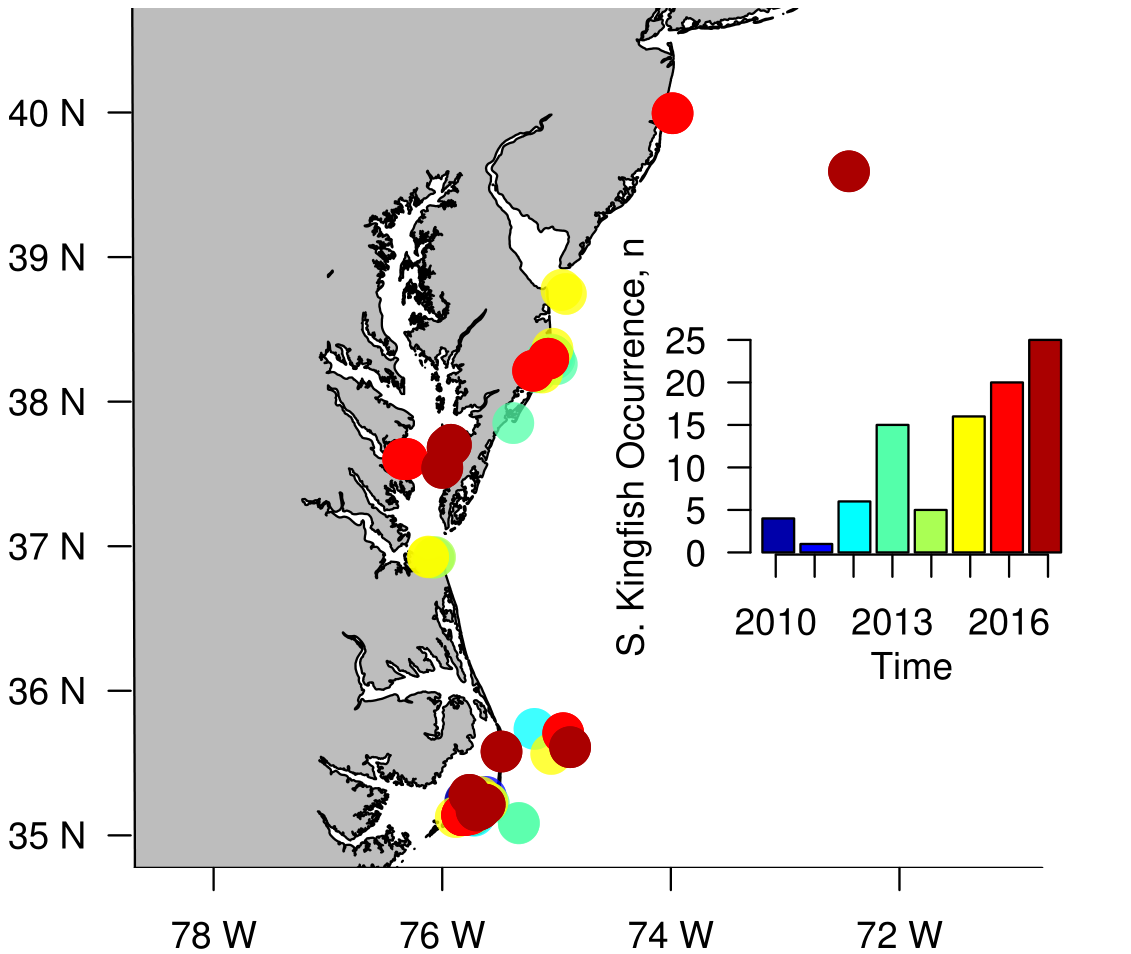
\includegraphics[width=15.71in]{C:/Users/kimberly.bastille/Desktop/tech-doc/images/southern_kingfish} 

}

\caption{Verified records of Southern Kingfish occurrence in the Mid-Atlantic.}\label{fig:SK-plot}
\end{figure}

\chapter{Habitat Occupancy Models}\label{habitat-occupancy-models}

\textbf{Description}: Habitat Occupancy

\textbf{Found in}: State of the Ecosystem - Gulf of Maine \& Georges
Bank (2018), State of the Ecosystem - Mid-Atlantic (2018)

\textbf{Indicator category}: Database pull with analysis; Extensive
analysis; not yet published; Published methods

\textbf{Contributor(s)}: Kevin Friedland

\textbf{Data steward}: Kevin Friedland,
\href{mailto:kevin.friedland@noaa.gov}{\nolinkurl{kevin.friedland@noaa.gov}}

\textbf{Point of contact}: Kevin Friedland,
\href{mailto:kevin.friedland@noaa.gov}{\nolinkurl{kevin.friedland@noaa.gov}}

\textbf{Public availability statement}: Source data are available upon
request (see \protect\hyperlink{survdat}{Survdat},
\protect\hyperlink{chl-pp}{CHL/PP}, and Data Sources below for more
information). Model-derived time series are available
\href{https://comet.nefsc.noaa.gov/erddap/tabledap/SOE_habitat_soe_v1.html}{here}.

\section{Methods}\label{methods-20}

Habitat area with a probability of occupancy greater than 0.5 was
modeled for many
\href{https://www.nefsc.noaa.gov/ecosys/current-conditions/occupancy-change.html}{species
throughout the NE-LME} using random forest decision tree models.

\subsection{Data sources}\label{data-sources-20}

Models were parameterized using a suite of static and dynamic predictor
variables, with occurrence and catch per unit effort (CPUE) of species
from spring and fall Northeast Fisheries Science Center (NEFSC) bottom
trawl surveys (BTS) serving as response variables. Sources of variables
used in the analyses are described below.

\subsubsection{Station depth}\label{station-depth}

The NEFSC BTS data included depth observations made concurrently with
trawls at each station. Station depth was a static variable for these
analyses.

\subsubsection{Ocean temperature and
salinity}\label{ocean-temperature-and-salinity}

Sea surface and bottom water temperature and salinity measurements were
included as dynamic predictor variables in the model, and were collected
using Conductivity/Temperature/Depth (CTD) instruments. Ocean
temperature and salinity measurements had the highest temporal coverage
during the spring (February-April) and fall (September-November) months.
Station salinity data were available between 1992-2016.

\subsubsection{Habitat descriptors}\label{habitat-descriptors}

A variety of benthic habitat descriptors were incorporated as predictor
variables in occupancy models (Table \ref{tab:habitatdesc}). The
majority of these parameters are based on depth (e.g. \emph{BPI},
\emph{VRM}, \emph{Prcury}, \emph{rugosity}, \emph{seabedforms},
\emph{slp}, and \emph{slpslp}). The vorticity variable is based on
current estimates, and the variable \emph{soft\_sed} based on sediment
grain size.

\begin{table}

\caption{\label{tab:habitatdesc}Habitat descriptors used in model parameterization.}
\centering
\begin{tabular}[t]{lll}
\toprule
Variables & Notes & References\\
\midrule
Namera\_vrm & Vector Ruggedness Measure (VRM) measures terrain ruggedness as the variation in three-dimensional orientation of grid cells within a neighborhood based the TNC Northwest Atlantic Marine Ecoregional Assessment ("NAMERA") data. & @Hobson1972; @Sappington2007\\
Prcurv (2 km, 10 km, and 20 km) & Benthic profile curvature at 2km, 10km and 20 km spatial scales was derived from depth data. & @Winship2018\\
Rugosity & A measure of small-scale variations of amplitude in the height of a surface, the ratio of the real to the geometric surface area. & @Friedman2012\\
seabedforms & Seabed topography as measured by a combination of seabed position and slope. & [http://www.northeastoceandata.org/](http://www.northeastoceandata.org/)\\
Slp (2 km, 10 km, and 20 km) & Benthic slope at 2km, 10km and 20km spatial scales. & @Winship2018\\
\addlinespace
Slpslp (2 km, 10 km, and 20 km) & Benthic slope of slope at 2km, 10km and 20km spatial scales & @Winship2018\\
soft\_sed & Soft-sediments is based on grain size distribution from the USGS usSeabed: Atlantic coast offshore surficial sediment data. & [http://www.northeastoceandata.org/](http://www.northeastoceandata.org/)\\
Vort (fall - fa; spring - sp; summer - su; winter - wi) & Benthic current vorticity at a 1/6 degree (approx. 19 km) spatial scale. & @Kinlan2016\\
\bottomrule
\end{tabular}
\end{table}

\subsubsection{Zooplankton}\label{zooplankton}

Zooplankton data are acquired through the NEFSC Ecosystem Monitoring
Program (``EcoMon''). For more information regarding the collection
process for these data, see Kane
(\protect\hyperlink{ref-Kane2007}{2007}), Kane
(\protect\hyperlink{ref-Kane2011}{2011}), and Morse et al.
(\protect\hyperlink{ref-Morse2017}{2017}). The bio-volume of the 18 most
abundant zooplankton taxa were considered as potential predictor
variables.

\subsubsection{Remote sensing data}\label{remote-sensing-data}

Both chlorophyll concentration and SST from remote sensing sources were
incorporated as static predictor variables in the model. During the
period of 1997-2016, chlorophyll concentrations were derived from
observations made by the Sea-viewing Wide Field of View Sensor
(SeaWIFS), Moderate Resolution Imaging Spectroradiometer (MODIS-Aqua),
Medium Resolution Imaging Spectrometer (MERIS), and Visible and Infrared
Imaging/Radiometer Suite (VIIRS).

\subsection{Data processing}\label{data-processing-11}

\subsubsection{Zooplankton}\label{zooplankton-1}

Missing values in the EcoMon time series were addressed by summing data
over five-year time steps for each seasonal time frame and interpolating
a complete field using ordinary kriging. Missing values necessitated
interpolation for spring data in 1989, 1990, 1991, and 1994. The same
was true of the fall data for 1989, 1990, and 1992.

\subsubsection{Remote sensing data}\label{remote-sensing-data-1}

An overlapping time series of observations from the four sensors listed
above was created using a bio-optical model inversion algorithm
(Maritorena et al. \protect\hyperlink{ref-Maritorena2010}{2010}).
Monthly SST data were derived from MODIS-Terra sensor data (available
\href{https://oceancolor.gsfc.nasa.gov/data/terra/}{here}).

\subsubsection{Ocean temperature and
salinity}\label{ocean-temperature-and-salinity-1}

Date of collection corrections for ocean temperature data were developed
using linear regressions for the spring and fall time frames;
standardizing to collection dates of April 3 and October 11 for spring
and fall. No correction was performed for salinity data. Annual data for
ocean temperature and salinity were combined with climatology by season
through an optimal interpolation approach. Specifically, mean bottom
temperature or salinity was calculated by year and season on a 0.5° grid
across the ecosystem, and data from grid cells with \textgreater{}80\%
temporal coverage were used to calculate a final seasonal mean. Annual
seasonal means were then used to calculate combined anomalies for
seasonal surface and bottom climatologies.

An annual field was then estimated using raw data observations for a
year, season, and depth using universal kriging (Hiemstra et al.
\protect\hyperlink{ref-automap}{2008}), with depth included as a
covariate (on a standard 0.1° grid). This field was then combined with
the climatology anomaly field and adjusted by the annual mean using the
variance field from kriging as the basis for a weighted mean between the
two. The variance field was divided into quartiles with the lowest
quartile assigned a weighting of 4:1 between the annual and climatology
values. The optimally interpolated field at these locations was
therefore skewed towards the annual data, reflecting their proximity to
actual data locations and associated low kriging variance. The highest
kriging variance quartile (1:1) reflected less information from the
annual field and more from the climatology.

\subsection{Data analysis}\label{data-analysis-18}

\subsubsection{Occupancy models}\label{occupancy-models}

Prior to fitting the occupancy models, predictor variables were tested
for multi-collinearity and removed if found to be correlated. The final
model variables were then chosen utilizing a model selection process as
shown by Murphy, Evans, and Storfer
(\protect\hyperlink{ref-Murphy2010}{2010}) and implemented with the R
package rfUtilities (Evans and Murphy
\protect\hyperlink{ref-rfUtilities-package}{2018}). Occupancy models
were then fit as two-factor classification models (absence as 0 and
presence as 1) using the randomForest R package (Liaw and Wiener
\protect\hyperlink{ref-randomForest}{2002}).

\subsubsection{Selection criteria and variable
importance}\label{selection-criteria-and-variable-importance}

The irr R package (Gamer, Lemon, and Singh
\protect\hyperlink{ref-irr}{2012}) was used to calculate Area Under the
ROC Curve (AUC) and Cohen's Kappa for assessing accuracy of occupancy
habitat models. Variable importance was assessed by plotting the
occurrence of a variable as a root variable versus the mean minimum node
depth for the variable (Paluszynska and Biecek
\protect\hyperlink{ref-randomForestExplainer}{2017}), as well as by
plotting the Gini index decrease versus accuracy decrease.

\subsection{Plotting}\label{plotting-13}

\begin{Shaded}
\begin{Highlighting}[]
\CommentTok{# Relative working directories}
\NormalTok{data.dir  <-}\StringTok{ }\NormalTok{here}\OperatorTok{::}\KeywordTok{here}\NormalTok{(}\StringTok{'data'}\NormalTok{)}
\NormalTok{r.dir <-}\StringTok{ }\NormalTok{here}\OperatorTok{::}\KeywordTok{here}\NormalTok{(}\StringTok{'R'}\NormalTok{)}

\CommentTok{# Load data}
\KeywordTok{load}\NormalTok{(}\KeywordTok{file.path}\NormalTok{(data.dir,}\StringTok{"SOE_data_erddap.Rdata"}\NormalTok{))}

\CommentTok{# Source plotting functions}
\KeywordTok{source}\NormalTok{(}\KeywordTok{file.path}\NormalTok{(r.dir,}\StringTok{"BasePlot_source.R"}\NormalTok{))}


\NormalTok{opar <-}\StringTok{ }\KeywordTok{par}\NormalTok{(}\DataTypeTok{mfrow =} \KeywordTok{c}\NormalTok{(}\DecValTok{2}\NormalTok{, }\DecValTok{1}\NormalTok{), }\DataTypeTok{mar =} \KeywordTok{c}\NormalTok{(}\DecValTok{0}\NormalTok{, }\DecValTok{0}\NormalTok{, }\DecValTok{0}\NormalTok{, }\DecValTok{0}\NormalTok{), }\DataTypeTok{oma =} \KeywordTok{c}\NormalTok{(}\FloatTok{3.5}\NormalTok{, }\DecValTok{5}\NormalTok{, }\DecValTok{2}\NormalTok{, }\DecValTok{4}\NormalTok{))}

\KeywordTok{soe.plot}\NormalTok{(SOE.data, }\StringTok{"Time"}\NormalTok{, }\StringTok{"sumflo spring habitat occupancy"}\NormalTok{, }\DataTypeTok{stacked =} \StringTok{"A"}\NormalTok{,}
         \DataTypeTok{rel.y.num =} \FloatTok{1.1}\NormalTok{, }\DataTypeTok{scale.axis =} \DecValTok{10}\OperatorTok{^}\DecValTok{3}\NormalTok{, }\DataTypeTok{end.start =} \DecValTok{2007}\NormalTok{, }\DataTypeTok{full.trend =}\NormalTok{ F,}
         \DataTypeTok{cex.stacked =} \FloatTok{1.5}\NormalTok{)}
\KeywordTok{soe.plot}\NormalTok{(SOE.data, }\StringTok{"Time"}\NormalTok{, }\StringTok{"sumflo fall habitat occupancy"}\NormalTok{, }\DataTypeTok{stacked =} \StringTok{"B"}\NormalTok{,}
         \DataTypeTok{rel.y.num =} \FloatTok{1.1}\NormalTok{, }\DataTypeTok{scale.axis =} \DecValTok{10}\OperatorTok{^}\DecValTok{3}\NormalTok{, }\DataTypeTok{end.start =} \DecValTok{2007}\NormalTok{, }\DataTypeTok{full.trend =}\NormalTok{ F,}
         \DataTypeTok{cex.stacked =} \FloatTok{1.5}\NormalTok{)}

\KeywordTok{soe.stacked.axis}\NormalTok{(}\StringTok{"Year"}\NormalTok{, }\KeywordTok{expression}\NormalTok{(}\StringTok{"Habitat Area, 10"}\OperatorTok{^}\DecValTok{3}\OperatorTok{*}\StringTok{" km"}\OperatorTok{^}\DecValTok{2}\NormalTok{), }\DataTypeTok{y.line =} \FloatTok{2.5}\NormalTok{)}
\end{Highlighting}
\end{Shaded}

\begin{figure}
\centering
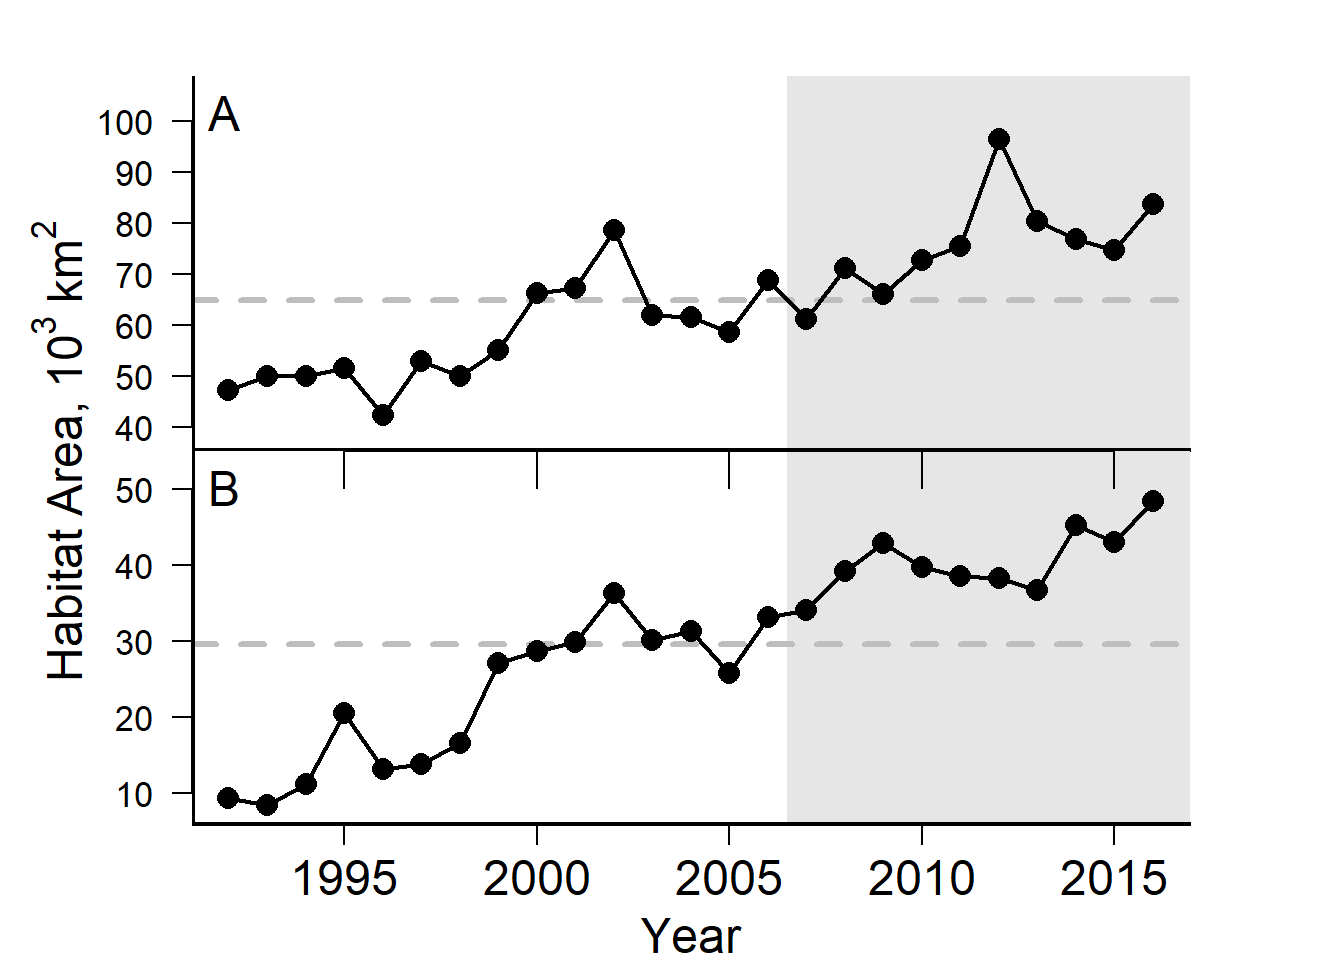
\includegraphics{C:/Users/kimberly.bastille/Desktop/tech-doc/imagesoccupancy-MAB-1.pdf}
\caption{\label{fig:occupancy-MAB}Summer flounder spring (A) and fall (B)
occupancy habitat area in the Northeast Large Marine Ecosystem.}
\end{figure}

\chapter{Fish Productivity Indicator}\label{fish-productivity-indicator}

\textbf{Description}: Groundfish productivity estimated as the ratio of
small fish to large fish

\textbf{Found in}: State of the Ecosystem - Gulf of Maine \& Georges
Bank (2017, 2018), State of the Ecosystem - Mid-Atlantic (2017, 2018,
2019)

\textbf{Indicator category}: Database pull with analysis; Published
methods

\textbf{Contributor(s)}: Charles Perretti

\textbf{Data steward}: Charles Perretti,
\href{mailto:charles.perretti@noaa.gov}{\nolinkurl{charles.perretti@noaa.gov}}

\textbf{Point of contact}: Charles Perretti,
\href{mailto:charles.perretti@noaa.gov}{\nolinkurl{charles.perretti@noaa.gov}}

\textbf{Public availability statement}: Source data are available upon
request.

\section{Methods}\label{methods-21}

\subsection{Data sources}\label{data-sources-21}

Survey data from NEFSC trawl database. These data in their derived form
are available through \protect\hyperlink{survdat}{Survdat}.

\subsection{Data extraction}\label{data-extraction-18}

Data were extracted from \protect\hyperlink{survdat}{Survdat}.

\subsection{Data analysis}\label{data-analysis-19}

We defined size thresholds separating small and large fish for each
species based on the 20th percentile of the length distribution across
all years. This threshold was then used to calculate a small and large
fish index (numbers below and above the threshold, respectively) each
year. Although the length percentile corresponding to age-1 fish will
vary with species, we use the 20th percentile as an approximation.
Biomass was calculated using length--weight relationships directly from
the survey data. Following Wigley, McBride, and McHugh
(\protect\hyperlink{ref-wigley_length-weight_2003}{2003}), the
length-weight relationship was modeled as \[\ln W = \ln a + b \ln L\]
where \(W\) is weight (kg), \(L\) is length (cm), and \(a\) and \(b\)
are parameters fit via linear regression. The ratio of small fish
numbers of the following year to larger fish biomass in the current year
was used as the index of recruitment success. The fall and spring
recruitment success anomalies were averaged to provide an annual index
of recruitment success.

Further details of methods described in Perretti et al.
(\protect\hyperlink{ref-perretti_regime_2017}{2017}\protect\hyperlink{ref-perretti_regime_2017}{a}).

\subsection{Data processing}\label{data-processing-12}

Productivity data were formatted for inclusion in the ecodata R package
using the following R code.

\begin{Shaded}
\begin{Highlighting}[]
\CommentTok{#processing small fish per large fish biomass indicator}

\KeywordTok{library}\NormalTok{(dplyr)}
\KeywordTok{library}\NormalTok{(tidyr)}
\KeywordTok{library}\NormalTok{(ggplot2)}

\NormalTok{raw.dir <-}\StringTok{ }\NormalTok{here}\OperatorTok{::}\KeywordTok{here}\NormalTok{(}\StringTok{"data-raw"}\NormalTok{)}

\KeywordTok{load}\NormalTok{(}\KeywordTok{file.path}\NormalTok{(raw.dir,}\StringTok{"dat_spec_rec_forSOE.Rdata"}\NormalTok{))}
\KeywordTok{load}\NormalTok{(}\KeywordTok{file.path}\NormalTok{(raw.dir,}\StringTok{"dat_spec_rec_epu_forSOE.Rdata"}\NormalTok{))}

\CommentTok{#Select and rename}
\NormalTok{epu_rec_anom <-}\StringTok{ }\NormalTok{dat_spec_rec_epu_forSOE }\OperatorTok\StringTok{ }
\StringTok{  }\NormalTok{dplyr}\OperatorTok{::}\KeywordTok{select}\NormalTok{(Time, }\DataTypeTok{EPU =}\NormalTok{ Region, Value, Units, }\OperatorTok{-}\NormalTok{Source,Var)}

\CommentTok{#Select, rename, and bind}
\NormalTok{productivity_anomaly <-}\StringTok{ }\NormalTok{dat_spec_rec_forSOE }\OperatorTok\StringTok{ }
\StringTok{  }\NormalTok{dplyr}\OperatorTok{::}\KeywordTok{select}\NormalTok{(}\OperatorTok{-}\NormalTok{Source) }\OperatorTok\StringTok{ }
\StringTok{  }\KeywordTok{mutate}\NormalTok{(}\DataTypeTok{EPU =} \StringTok{"All"}\NormalTok{,}
         \DataTypeTok{Var =} \KeywordTok{paste}\NormalTok{(}\StringTok{"NE LME"}\NormalTok{,Var)) }\OperatorTok\StringTok{ }
\StringTok{  }\KeywordTok{rbind}\NormalTok{(.,epu_rec_anom) }\OperatorTok\StringTok{ }
\StringTok{  }\KeywordTok{as.data.frame}\NormalTok{()}

\NormalTok{usethis}\OperatorTok{::}\KeywordTok{use_data}\NormalTok{(productivity_anomaly, }\DataTypeTok{overwrite =} \OtherTok{TRUE}\NormalTok{)}
\end{Highlighting}
\end{Shaded}

\subsection{Plotting}\label{plotting-14}

\begin{Shaded}
\begin{Highlighting}[]
\CommentTok{# Relative working directories}
\NormalTok{data.dir  <-}\StringTok{ }\NormalTok{here}\OperatorTok{::}\KeywordTok{here}\NormalTok{(}\StringTok{'data'}\NormalTok{)}
\NormalTok{r.dir <-}\StringTok{ }\NormalTok{here}\OperatorTok{::}\KeywordTok{here}\NormalTok{(}\StringTok{'R'}\NormalTok{)}

\CommentTok{# Load data}
\KeywordTok{load}\NormalTok{(}\KeywordTok{file.path}\NormalTok{(data.dir,}\StringTok{"SOE_data_erddap.Rdata"}\NormalTok{))}

\NormalTok{#### Functions for plotting ####}
\KeywordTok{library}\NormalTok{(ggplot2)}
\KeywordTok{library}\NormalTok{(rpart)}
\KeywordTok{library}\NormalTok{(dplyr)}
\KeywordTok{library}\NormalTok{(stringr)}

\NormalTok{all_epu <-}\StringTok{ }\NormalTok{SOE.data }\OperatorTok
\StringTok{  }\KeywordTok{filter}\NormalTok{(}\KeywordTok{str_detect}\NormalTok{(Var, }\StringTok{"All EPU productivity"}\NormalTok{))}

\NormalTok{all_epu}\OperatorTok{$}\NormalTok{Var <-}\StringTok{ }\KeywordTok{str_trim}\NormalTok{(}\KeywordTok{str_replace}\NormalTok{(all_epu}\OperatorTok{$}\NormalTok{Var, }\StringTok{"All EPU productivity"}\NormalTok{,}\StringTok{""}\NormalTok{))}


\CommentTok{# Adjust plot properties}
\NormalTok{adjustAxes <-}\StringTok{ }
\StringTok{  }\NormalTok{ggplot2}\OperatorTok{::}\KeywordTok{theme}\NormalTok{(}\DataTypeTok{axis.title   =} \KeywordTok{element_text}\NormalTok{(}\DataTypeTok{size =} \DecValTok{18}\NormalTok{),}
                 \DataTypeTok{axis.text    =} \KeywordTok{element_text}\NormalTok{(}\DataTypeTok{size =} \DecValTok{15}\NormalTok{),}
                 \DataTypeTok{plot.title   =} \KeywordTok{element_text}\NormalTok{(}\DataTypeTok{size =} \DecValTok{20}\NormalTok{))}

\NormalTok{ggplot <-}\StringTok{ }\ControlFlowTok{function}\NormalTok{(...) \{ ggplot2}\OperatorTok{::}\KeywordTok{ggplot}\NormalTok{(...)  }\OperatorTok{+}\StringTok{ }
\StringTok{    }\NormalTok{ggplot2}\OperatorTok{::}\KeywordTok{theme_bw}\NormalTok{() }\OperatorTok{+}\StringTok{ }
\StringTok{    }\NormalTok{adjustAxes\}}


\CommentTok{# Plot stacked bar with cpts for single var }
\NormalTok{plot_stackbarcpts_single <-}\StringTok{ }\ControlFlowTok{function}\NormalTok{(YEAR, var2bar,}
\NormalTok{                                     x, xlab, ylab,}
\NormalTok{                                     titl,}
\NormalTok{                                     file_suffix,}
                                     \DataTypeTok{leg_font_size =} \DecValTok{10}\NormalTok{,}
                                     \DataTypeTok{remove_leg =} \OtherTok{FALSE}\NormalTok{,}
                                     \DataTypeTok{leg_ncol =} \DecValTok{1}\NormalTok{,}
                                     \DataTypeTok{wcpts =} \OtherTok{TRUE}\NormalTok{,}
                                     \DataTypeTok{wdashed =} \OtherTok{TRUE}\NormalTok{,}
                                     \DataTypeTok{height =} \FloatTok{5.5}\NormalTok{,}
                                     \DataTypeTok{width =} \DecValTok{8}\NormalTok{) \{}
  
\NormalTok{  dat2bar <-}\StringTok{ }\KeywordTok{data.frame}\NormalTok{(YEAR, var2bar,}
\NormalTok{                        x)}
  
\NormalTok{  dat2plot <-}
\StringTok{    }\NormalTok{dat2bar }\OperatorTok
\StringTok{    }\NormalTok{tidyr}\OperatorTok{::}\KeywordTok{gather}\NormalTok{(variable, value, }\OperatorTok{-}\NormalTok{YEAR, }\OperatorTok{-}\NormalTok{var2bar) }\OperatorTok
\StringTok{    }\NormalTok{dplyr}\OperatorTok{::}\KeywordTok{mutate}\NormalTok{(}\DataTypeTok{var2bar =} \KeywordTok{gsub}\NormalTok{(}\DataTypeTok{pattern      =} \StringTok{"_"}\NormalTok{, }
                                 \DataTypeTok{replacement  =} \StringTok{" "}\NormalTok{, }
                                 \DataTypeTok{x            =}\NormalTok{ var2bar),}
                  \DataTypeTok{var2bar =} \KeywordTok{gsub}\NormalTok{(}\DataTypeTok{pattern      =} \StringTok{"Atl."}\NormalTok{, }
                                 \DataTypeTok{replacement  =} \StringTok{""}\NormalTok{, }
                                 \DataTypeTok{x            =}\NormalTok{ var2bar),}
                  \DataTypeTok{var2bar =} \KeywordTok{gsub}\NormalTok{(}\DataTypeTok{pattern      =} \StringTok{"Atl"}\NormalTok{, }
                                 \DataTypeTok{replacement  =} \StringTok{""}\NormalTok{, }
                                 \DataTypeTok{x            =}\NormalTok{ var2bar),}
                  \DataTypeTok{var2bar =} \KeywordTok{gsub}\NormalTok{(}\DataTypeTok{pattern      =} \StringTok{"NS and combined"}\NormalTok{, }
                                 \DataTypeTok{replacement  =} \StringTok{""}\NormalTok{, }
                                 \DataTypeTok{x            =}\NormalTok{ var2bar),}
                  \DataTypeTok{var2bar =} \KeywordTok{gsub}\NormalTok{(}\DataTypeTok{pattern      =} \StringTok{"YT"}\NormalTok{, }
                                 \DataTypeTok{replacement  =} \StringTok{"Yellowtail"}\NormalTok{, }
                                 \DataTypeTok{x            =}\NormalTok{ var2bar),}
                  \DataTypeTok{var2bar =} \KeywordTok{gsub}\NormalTok{(}\DataTypeTok{pattern      =} \StringTok{" GoM"}\NormalTok{, }
                                 \DataTypeTok{replacement  =} \StringTok{" GOM"}\NormalTok{, }
                                 \DataTypeTok{x            =}\NormalTok{ var2bar))}
  
  
\NormalTok{  p <-}\StringTok{   }
\StringTok{    }\KeywordTok{ggplot}\NormalTok{(dat2plot,}
           \KeywordTok{aes}\NormalTok{(}\DataTypeTok{x =}\NormalTok{ YEAR)) }\OperatorTok{+}
\StringTok{    }\KeywordTok{geom_bar}\NormalTok{(}\DataTypeTok{data =}\NormalTok{ dat2plot }\OperatorTok\StringTok{ }\KeywordTok{filter}\NormalTok{(value }\OperatorTok{>}\StringTok{ }\DecValTok{0}\NormalTok{),}
             \KeywordTok{aes}\NormalTok{(}\DataTypeTok{y =}\NormalTok{ value, }\DataTypeTok{fill =}\NormalTok{ var2bar),}
             \DataTypeTok{stat =} \StringTok{"identity"}\NormalTok{) }\OperatorTok{+}
\StringTok{    }\KeywordTok{geom_bar}\NormalTok{(}\DataTypeTok{data =}\NormalTok{ dat2plot }\OperatorTok\StringTok{ }\KeywordTok{filter}\NormalTok{(value }\OperatorTok{<}\StringTok{ }\DecValTok{0}\NormalTok{),}
             \KeywordTok{aes}\NormalTok{(}\DataTypeTok{y =}\NormalTok{ value, }\DataTypeTok{fill =}\NormalTok{ var2bar),}
             \DataTypeTok{stat =} \StringTok{"identity"}\NormalTok{) }\OperatorTok{+}
\StringTok{    }\KeywordTok{geom_hline}\NormalTok{(}\DataTypeTok{size =} \FloatTok{0.3}\NormalTok{, }\KeywordTok{aes}\NormalTok{(}\DataTypeTok{yintercept =} \DecValTok{0}\NormalTok{)) }\OperatorTok{+}
\StringTok{    }\KeywordTok{xlab}\NormalTok{(xlab) }\OperatorTok{+}
\StringTok{    }\KeywordTok{ylab}\NormalTok{(ylab) }\OperatorTok{+}
\StringTok{    }\KeywordTok{ggtitle}\NormalTok{(titl) }\OperatorTok{+}
\StringTok{    }\KeywordTok{guides}\NormalTok{(}\DataTypeTok{fill =} \KeywordTok{guide_legend}\NormalTok{(}\DataTypeTok{ncol =}\NormalTok{ leg_ncol)) }\OperatorTok{+}
\StringTok{    }\KeywordTok{theme}\NormalTok{(}\DataTypeTok{axis.title   =} \KeywordTok{element_text}\NormalTok{(}\DataTypeTok{size =} \DecValTok{16}\NormalTok{),}
          \DataTypeTok{axis.text    =} \KeywordTok{element_text}\NormalTok{(}\DataTypeTok{size =} \DecValTok{15}\NormalTok{),}
          \DataTypeTok{plot.title   =} \KeywordTok{element_text}\NormalTok{(}\DataTypeTok{size =} \DecValTok{20}\NormalTok{),}
          \DataTypeTok{legend.text  =} \KeywordTok{element_text}\NormalTok{(}\DataTypeTok{size =}\NormalTok{ leg_font_size),}
          \DataTypeTok{legend.title =} \KeywordTok{element_blank}\NormalTok{())}
  
  \ControlFlowTok{if}\NormalTok{(remove_leg) p <-}\StringTok{ }\NormalTok{p }\OperatorTok{+}\StringTok{ }\KeywordTok{theme}\NormalTok{(}\DataTypeTok{legend.position =} \StringTok{"none"}\NormalTok{)}
  
  \KeywordTok{print}\NormalTok{(p)}
  
\CommentTok{#  ggsave(plot = p,}
\CommentTok{#         filename = "./productivity_all.eps",}
\CommentTok{#         width = width,}
\CommentTok{#         height = height)}
\NormalTok{\}}

\CommentTok{# Plot stacked bars}
\NormalTok{plot_stackbarcpts <-}\StringTok{ }\ControlFlowTok{function}\NormalTok{(YEAR, var2bar,}
\NormalTok{                              top, mid, bot,}
\NormalTok{                              top_lab, }
\NormalTok{                              mid_lab, }
\NormalTok{                              bot_lab,}
                              \DataTypeTok{xlab =} \StringTok{""}\NormalTok{, }
                              \DataTypeTok{ylab =} \StringTok{""}\NormalTok{,}
                              \DataTypeTok{titl =} \StringTok{""}\NormalTok{) \{}
  
\NormalTok{  dat2bar <-}\StringTok{ }\KeywordTok{data.frame}\NormalTok{(YEAR, var2bar,}
\NormalTok{                        top, mid, }
\NormalTok{                        bot)}
  
\NormalTok{  dat2plot <-}
\StringTok{    }\NormalTok{dat2bar }\OperatorTok
\StringTok{    }\NormalTok{tidyr}\OperatorTok{::}\KeywordTok{gather}\NormalTok{(variable, value, }\OperatorTok{-}\NormalTok{YEAR, }\OperatorTok{-}\NormalTok{var2bar) }\OperatorTok
\StringTok{    }\NormalTok{dplyr}\OperatorTok{::}\KeywordTok{mutate}\NormalTok{(}\DataTypeTok{variable =} \KeywordTok{ifelse}\NormalTok{(variable }\OperatorTok{==}\StringTok{ "top"}\NormalTok{, }
\NormalTok{                                    top_lab, }
                                    \KeywordTok{ifelse}\NormalTok{(variable }\OperatorTok{==}\StringTok{ "mid"}\NormalTok{,}
\NormalTok{                                           mid_lab, bot_lab)))}
  
  
\NormalTok{  dat2plot}\OperatorTok{$}\NormalTok{variable <-}\StringTok{ }
\StringTok{    }\KeywordTok{factor}\NormalTok{(dat2plot}\OperatorTok{$}\NormalTok{variable,}
           \DataTypeTok{levels =} \KeywordTok{c}\NormalTok{(top_lab, mid_lab, bot_lab))}
  
\NormalTok{  p <-}\StringTok{   }
\StringTok{    }\KeywordTok{ggplot}\NormalTok{(dat2plot,}
           \KeywordTok{aes}\NormalTok{(}\DataTypeTok{x =}\NormalTok{ YEAR)) }\OperatorTok{+}
\StringTok{    }\KeywordTok{geom_bar}\NormalTok{(}\DataTypeTok{data =}\NormalTok{ dat2plot }\OperatorTok\StringTok{ }\KeywordTok{filter}\NormalTok{(value }\OperatorTok{>}\StringTok{ }\DecValTok{0}\NormalTok{),}
             \KeywordTok{aes}\NormalTok{(}\DataTypeTok{y =}\NormalTok{ value, }\DataTypeTok{fill =}\NormalTok{ var2bar),}
             \DataTypeTok{stat =} \StringTok{"identity"}\NormalTok{) }\OperatorTok{+}
\StringTok{    }\KeywordTok{geom_bar}\NormalTok{(}\DataTypeTok{data =}\NormalTok{ dat2plot }\OperatorTok\StringTok{ }\KeywordTok{filter}\NormalTok{(value }\OperatorTok{<}\StringTok{ }\DecValTok{0}\NormalTok{),}
             \KeywordTok{aes}\NormalTok{(}\DataTypeTok{y =}\NormalTok{ value, }\DataTypeTok{fill =}\NormalTok{ var2bar),}
             \DataTypeTok{stat =} \StringTok{"identity"}\NormalTok{) }\OperatorTok{+}
\StringTok{    }\KeywordTok{facet_wrap}\NormalTok{(}\OperatorTok{~}\StringTok{ }\NormalTok{variable, }\DataTypeTok{ncol =} \DecValTok{1}\NormalTok{) }\OperatorTok{+}
\StringTok{    }\KeywordTok{geom_hline}\NormalTok{(}\DataTypeTok{size =} \FloatTok{0.3}\NormalTok{, }\KeywordTok{aes}\NormalTok{(}\DataTypeTok{yintercept =} \DecValTok{0}\NormalTok{)) }\OperatorTok{+}
\StringTok{    }\KeywordTok{xlab}\NormalTok{(xlab) }\OperatorTok{+}
\StringTok{    }\KeywordTok{ylab}\NormalTok{(ylab) }\OperatorTok{+}
\StringTok{    }\KeywordTok{ggtitle}\NormalTok{(titl) }\OperatorTok{+}
\StringTok{    }\KeywordTok{guides}\NormalTok{(}\DataTypeTok{fill =} \KeywordTok{guide_legend}\NormalTok{(}\DataTypeTok{ncol =} \DecValTok{1}\NormalTok{)) }\OperatorTok{+}
\StringTok{    }\KeywordTok{theme}\NormalTok{(}\DataTypeTok{axis.title   =} \KeywordTok{element_text}\NormalTok{(}\DataTypeTok{size =} \DecValTok{16}\NormalTok{),}
          \DataTypeTok{axis.text    =} \KeywordTok{element_text}\NormalTok{(}\DataTypeTok{size =} \DecValTok{15}\NormalTok{),}
          \DataTypeTok{plot.title   =} \KeywordTok{element_text}\NormalTok{(}\DataTypeTok{size =} \DecValTok{20}\NormalTok{),}
          \DataTypeTok{strip.text   =} \KeywordTok{element_text}\NormalTok{(}\DataTypeTok{size =} \DecValTok{15}\NormalTok{),}
          \DataTypeTok{legend.title =} \KeywordTok{element_blank}\NormalTok{())}
  
  \KeywordTok{print}\NormalTok{(p)}
\NormalTok{\}}

\CommentTok{# Recruit per spawner (all stocks in one figure)}
\KeywordTok{plot_stackbarcpts_single}\NormalTok{(}\DataTypeTok{YEAR =}\NormalTok{ all_epu}\OperatorTok{$}\NormalTok{Time,}
                         \DataTypeTok{var2bar =}\NormalTok{ all_epu}\OperatorTok{$}\NormalTok{Var,}
                         \DataTypeTok{x =}\NormalTok{ all_epu}\OperatorTok{$}\NormalTok{Value,}
                         \DataTypeTok{titl =} \StringTok{""}\NormalTok{,}
                         \DataTypeTok{xlab =} \StringTok{""}\NormalTok{,}
                         \DataTypeTok{ylab =} \StringTok{"Small fish per large fish biomass (anomaly)"}\NormalTok{,}
                         \DataTypeTok{height =} \DecValTok{7}\NormalTok{,}
                         \DataTypeTok{width =} \DecValTok{9}\NormalTok{)}
\end{Highlighting}
\end{Shaded}

\begin{figure}
\centering
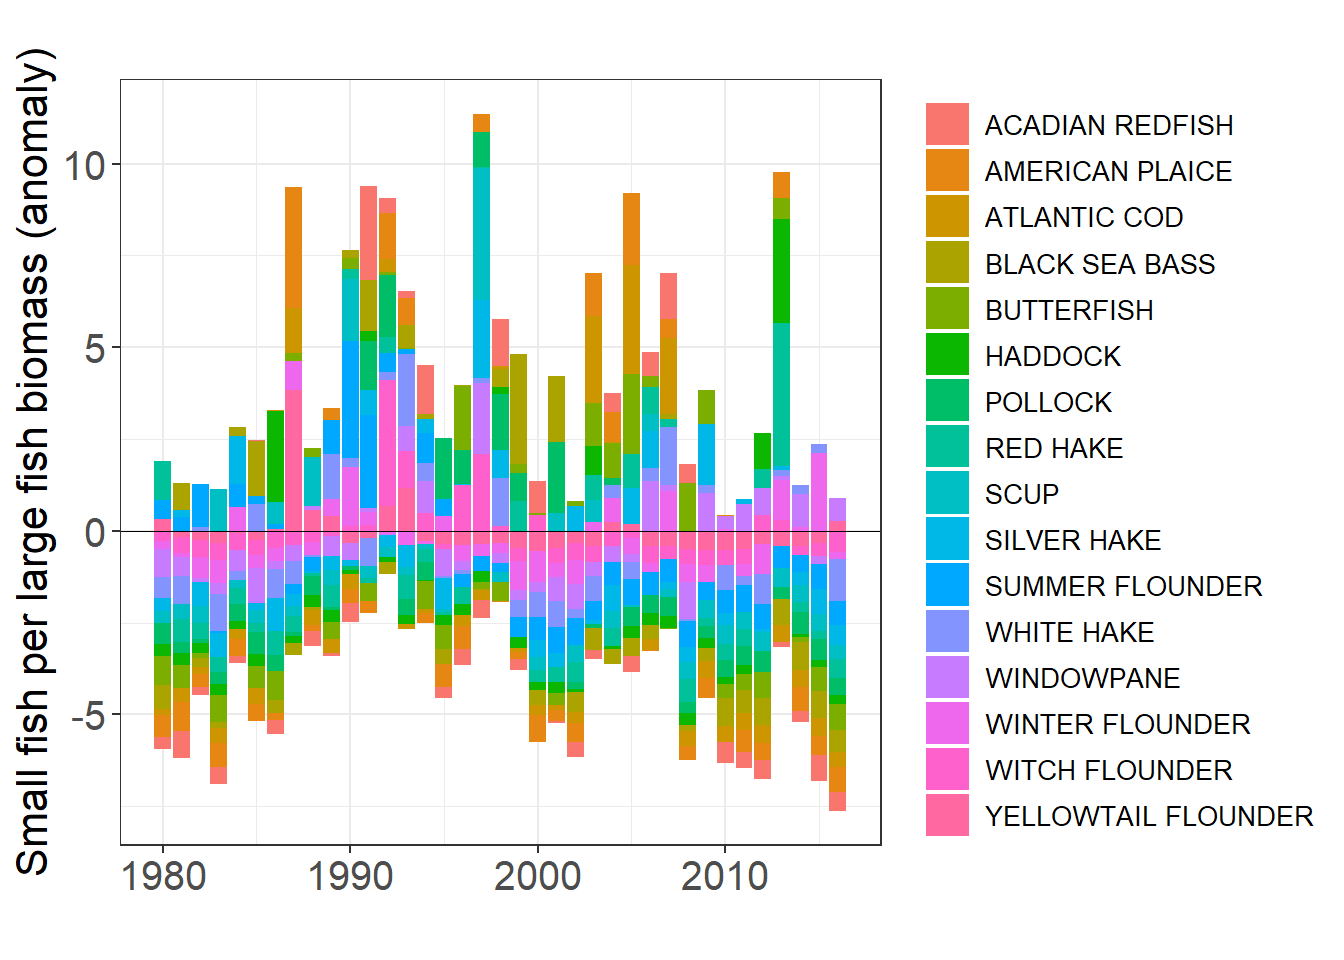
\includegraphics{C:/Users/kimberly.bastille/Desktop/tech-doc/imagesunnamed-chunk-45-1.pdf}
\caption{\label{fig:unnamed-chunk-45}Groundfish productivity across all
stocks in the Northeast Large Marine Ecosystem.}
\end{figure}

\begin{figure}
\centering
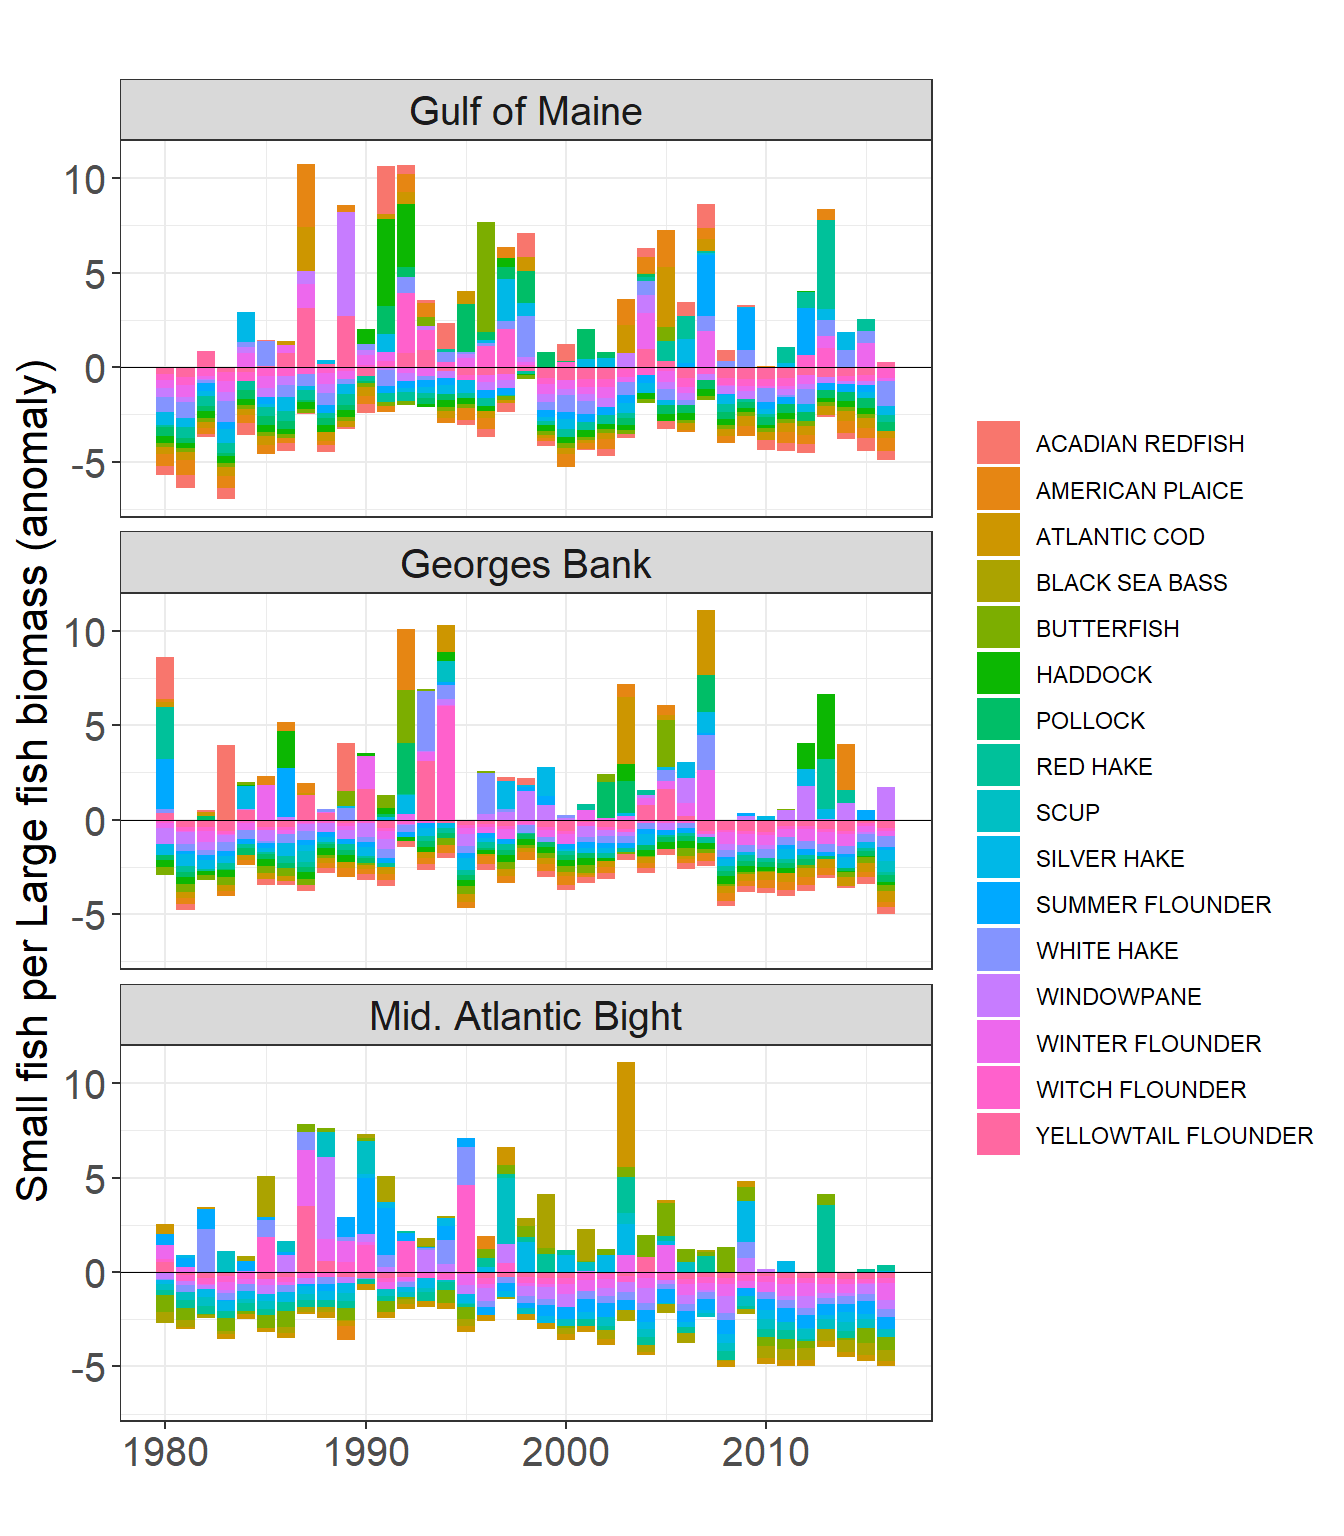
\includegraphics{C:/Users/kimberly.bastille/Desktop/tech-doc/imagesplot-all-1.pdf}
\caption{\label{fig:plot-all}Groundfish productivity visualized by EPU.}
\end{figure}

\chapter{Recreational Fishing
Indicators}\label{recreational-fishing-indicators}

\textbf{Description}: A variety of indicators derived from MRIP
Recreational Fisheries Statistics, including total recreational catch,
total angler trips by region, annual diversity of recreational fleet
effort, and annual diversity of managed species.

\textbf{Found in}: State of the Ecosystem - Gulf of Maine \& Georges
Bank (2017, 2018, 2019), State of the Ecosystem - Mid-Atlantic (2017,
2018, 2019)

\textbf{Indicator category}: Database pull with analysis

\textbf{Contributor(s)}: Geret DePiper, Scott Steinbeck

\textbf{Data steward}: Geret DePiper,
\href{mailto:geret.depiper@noaa.gov}{\nolinkurl{geret.depiper@noaa.gov}}

\textbf{Point of contact}: Geret DePiper,
\href{mailto:geret.depiper@noaa.gov}{\nolinkurl{geret.depiper@noaa.gov}}

\textbf{Public availability statement}: Data sets are publicly available
(see Data Sources below).

\section{Methods}\label{methods-22}

We used total recreational harvest as an indicator of seafood production
and total recreational trips and total recreational anglers as proxies
for recreational value generated from the Mid-Atlantic and New England
regions respectively. We estimated both recreational catch diversity in
managed species (MAFMC, NEFMC, and ASMFC) and fleet effort diversity
using the effective Shannon index.

\subsection{Data sources}\label{data-sources-22}

All recreational fishing indicator data, including number of
recreationally harvested fish, number of angler trips, and number of
anglers, were downloaded from the
\href{https://www.st.nmfs.noaa.gov/recreational-fisheries/data-and-documentation/queries/index}{MRIP
Recreational Fisheries Statistics Queries} portal. Relevant metadata
including information regarding data methodology updates are available
at the query site. Note that 2017 data were considered preliminary at
the time of the data pull.

Data sets were queried by region on the MRIP site, and for the purposes
of the SOE, the ``NORTH ATLANTIC'' and ``MID-ATLANTIC'' regions were
mapped to the New England and Mid-Atlantic report versions respectively.
All query pages are accessible through the
\href{https://www.st.nmfs.noaa.gov/recreational-fisheries/data-and-documentation/queries/index}{MRIP
Recreational Fisheries Statistics} site.

The number of recreationally harvested fish was found by selecting
``TOTAL HARVEST (A + B1)'' on the
\href{https://www.st.nmfs.noaa.gov/recreational-fisheries/data-and-documentation/run-a-data-query}{Catch
Time Series Query} page. Catch diversity estimates were also derived
from the total catch time series (see below). Species included in the
diversity of catch analysis included American eel, Atlantic cod,
Atlantic mackerel, Atlantic sturgeon, black drum, black sea bass,
bluefish, cobia, haddock, pollock, red drum, scup, Spanish mackerel,
spiny dogfish, spot, spotted seatrout, striped bass, summer flounder,
tautog, tilefish, weakfish, winter flounder, and ``All Other Species''.

Angler trips (listed as ``TOTAL'' trips) were pulled from the MRIP
\href{https://www.st.nmfs.noaa.gov/recreational-fisheries/data-and-documentation/run-a-data-query}{Effort
Time Series Query} page, and included data from 1981 - 2019. Time series
of recreational fleet effort diversity were calculated from this data
set (see below). The number of anglers was total number of anglers from
the MRFSS Participation Time Series Query, and includes data from 1981 -
2016.

\subsection{Data analysis}\label{data-analysis-20}

\textbf{Recreational fleet effort diversity}

\begin{Shaded}
\begin{Highlighting}[]
\NormalTok{REC_DATA <-}\StringTok{ }\KeywordTok{read.csv}\NormalTok{(}\StringTok{'X:/gdepiper/ESR2018/SOE/Data/Rec_Days_Fished_2018.csv'}\NormalTok{, }\DataTypeTok{as.is=}\OtherTok{TRUE}\NormalTok{)}

\NormalTok{REC_DATA}\OperatorTok{$}\NormalTok{P_Shore <-}\StringTok{ }\OperatorTok{-}\NormalTok{(}\KeywordTok{as.numeric}\NormalTok{(}\KeywordTok{gsub}\NormalTok{(}\StringTok{""}\NormalTok{,}\StringTok{""}\NormalTok{,}\StringTok{'""'}\NormalTok{,REC_DATA}\OperatorTok{$}\NormalTok{Shore)) }\OperatorTok{/}
\StringTok{                        }\KeywordTok{as.numeric}\NormalTok{(}\KeywordTok{gsub}\NormalTok{(}\StringTok{""}\NormalTok{,}\StringTok{""}\NormalTok{,}\StringTok{'""'}\NormalTok{,REC_DATA}\OperatorTok{$}\NormalTok{All_Modes))) }\OperatorTok{*}
\StringTok{                          }\KeywordTok{log}\NormalTok{(}\KeywordTok{as.numeric}\NormalTok{(}\KeywordTok{gsub}\NormalTok{(}\StringTok{""}\NormalTok{,}\StringTok{""}\NormalTok{,}\StringTok{'""'}\NormalTok{,REC_DATA}\OperatorTok{$}\NormalTok{Shore)) }\OperatorTok{/}
\StringTok{                                }\KeywordTok{as.numeric}\NormalTok{(}\KeywordTok{gsub}\NormalTok{(}\StringTok{""}\NormalTok{,}\StringTok{""}\NormalTok{,}\StringTok{'""'}\NormalTok{,REC_DATA}\OperatorTok{$}\NormalTok{All_Modes)))}

\NormalTok{REC_DATA}\OperatorTok{$}\NormalTok{P_Private <-}\StringTok{ }\OperatorTok{-}\NormalTok{(}\KeywordTok{as.numeric}\NormalTok{(}\KeywordTok{gsub}\NormalTok{(}\StringTok{""}\NormalTok{,}\StringTok{""}\NormalTok{,}\StringTok{'""'}\NormalTok{,REC_DATA}\OperatorTok{$}\NormalTok{Private_Rental)) }\OperatorTok{/}
\StringTok{                          }\KeywordTok{as.numeric}\NormalTok{(}\KeywordTok{gsub}\NormalTok{(}\StringTok{""}\NormalTok{,}\StringTok{""}\NormalTok{,}\StringTok{'""'}\NormalTok{,REC_DATA}\OperatorTok{$}\NormalTok{All_Modes))) }\OperatorTok{*}
\StringTok{                          }\KeywordTok{log}\NormalTok{(}\KeywordTok{as.numeric}\NormalTok{(}\KeywordTok{gsub}\NormalTok{(}\StringTok{""}\NormalTok{,}\StringTok{""}\NormalTok{,}\StringTok{'""'}\NormalTok{,REC_DATA}\OperatorTok{$}\NormalTok{Private_Rental)) }\OperatorTok{/}
\StringTok{                                }\KeywordTok{as.numeric}\NormalTok{(}\KeywordTok{gsub}\NormalTok{(}\StringTok{""}\NormalTok{,}\StringTok{""}\NormalTok{,}\StringTok{'""'}\NormalTok{,REC_DATA}\OperatorTok{$}\NormalTok{All_Modes)))}

\NormalTok{REC_DATA}\OperatorTok{$}\NormalTok{P_Party <-}\StringTok{ }\OperatorTok{-}\NormalTok{(}\KeywordTok{as.numeric}\NormalTok{(}\KeywordTok{gsub}\NormalTok{(}\StringTok{""}\NormalTok{,}\StringTok{""}\NormalTok{,}\StringTok{'""'}\NormalTok{,REC_DATA}\OperatorTok{$}\NormalTok{Party_Charter)) }\OperatorTok{/}
\StringTok{                        }\KeywordTok{as.numeric}\NormalTok{(}\KeywordTok{gsub}\NormalTok{(}\StringTok{""}\NormalTok{,}\StringTok{""}\NormalTok{,}\StringTok{'""'}\NormalTok{,REC_DATA}\OperatorTok{$}\NormalTok{All_Modes))) }\OperatorTok{*}
\StringTok{                        }\KeywordTok{log}\NormalTok{(}\KeywordTok{as.numeric}\NormalTok{(}\KeywordTok{gsub}\NormalTok{(}\StringTok{""}\NormalTok{,}\StringTok{""}\NormalTok{,}\StringTok{'""'}\NormalTok{,REC_DATA}\OperatorTok{$}\NormalTok{Party_Charter)) }\OperatorTok{/}
\StringTok{                              }\KeywordTok{as.numeric}\NormalTok{(}\KeywordTok{gsub}\NormalTok{(}\StringTok{""}\NormalTok{,}\StringTok{""}\NormalTok{,}\StringTok{'""'}\NormalTok{,REC_DATA}\OperatorTok{$}\NormalTok{All_Modes)))}

\NormalTok{REC_DATA}\OperatorTok{$}\NormalTok{Value <-}\StringTok{ }\KeywordTok{exp}\NormalTok{(REC_DATA}\OperatorTok{$}\NormalTok{P_Shore}\OperatorTok{+}\NormalTok{REC_DATA}\OperatorTok{$}\NormalTok{P_Private}\OperatorTok{+}\NormalTok{REC_DATA}\OperatorTok{$}\NormalTok{P_Party)}

\NormalTok{REC_DATA}\OperatorTok{$}\NormalTok{Region[REC_DATA}\OperatorTok{$}\NormalTok{Region}\OperatorTok{==}\StringTok{'"MID-ATLANTIC"'}\NormalTok{] <-}\StringTok{ 'MA'}
\NormalTok{REC_DATA}\OperatorTok{$}\NormalTok{Region[REC_DATA}\OperatorTok{$}\NormalTok{Region}\OperatorTok{==}\StringTok{'"NORTH ATLANTIC"'}\NormalTok{] <-}\StringTok{ 'NE'}

\NormalTok{E_SHANNON <-}\StringTok{ }\KeywordTok{subset}\NormalTok{(REC_DATA, }\DataTypeTok{select=}\KeywordTok{c}\NormalTok{(}\StringTok{'Time'}\NormalTok{,}\StringTok{'Region'}\NormalTok{,}\StringTok{'Value'}\NormalTok{))}
\NormalTok{E_SHANNON}\OperatorTok{$}\NormalTok{Units <-}\StringTok{ 'Effective Shannon'}
\NormalTok{E_SHANNON}\OperatorTok{$}\NormalTok{Var <-}\StringTok{ 'Recreational fleet effort diversity across modes'}
\NormalTok{E_SHANNON}\OperatorTok{$}\NormalTok{Source <-}\StringTok{ 'MRIP effort time series, processed to generate diversity measure.'}
\end{Highlighting}
\end{Shaded}

\textbf{Recreational catch diversity}

\begin{Shaded}
\begin{Highlighting}[]
\NormalTok{ REC_CATCH <-}\StringTok{ }\KeywordTok{read.csv}\NormalTok{(}\StringTok{'X:/gdepiper/ESR2018/SOE/Data/Rec_Species_Quantity_2018.csv'}\NormalTok{, }\DataTypeTok{as.is=}\OtherTok{TRUE}\NormalTok{)}

\NormalTok{REC_CATCH}\OperatorTok{$}\NormalTok{Value <-}\StringTok{  }\KeywordTok{as.numeric}\NormalTok{(}\KeywordTok{gsub}\NormalTok{(}\StringTok{","}\NormalTok{,}\StringTok{""}\NormalTok{,REC_CATCH}\OperatorTok{$}\NormalTok{Value))}
\NormalTok{TOT_REC_CATCH <-}\StringTok{ }\KeywordTok{aggregate}\NormalTok{(Value}\OperatorTok{~}\NormalTok{Time}\OperatorTok{+}\NormalTok{Region, }\DataTypeTok{data=}\NormalTok{REC_CATCH, }\DataTypeTok{FUN=}\NormalTok{sum)}
\KeywordTok{names}\NormalTok{(TOT_REC_CATCH) <-}\StringTok{ }\KeywordTok{c}\NormalTok{(}\StringTok{'Time'}\NormalTok{,}\StringTok{'Region'}\NormalTok{,}\StringTok{'Tot_Catch'}\NormalTok{)}
\NormalTok{REC_CATCH <-}\StringTok{ }\KeywordTok{merge}\NormalTok{(REC_CATCH,TOT_REC_CATCH, }\DataTypeTok{by=}\KeywordTok{c}\NormalTok{(}\StringTok{'Time'}\NormalTok{,}\StringTok{'Region'}\NormalTok{))}
\NormalTok{REC_CATCH}\OperatorTok{$}\NormalTok{P_Catch <-}\StringTok{ }\OperatorTok{-}\NormalTok{(REC_CATCH}\OperatorTok{$}\NormalTok{Value}\OperatorTok{/}\NormalTok{REC_CATCH}\OperatorTok{$}\NormalTok{Tot_Catch}\OperatorTok{*}
\KeywordTok{log}\NormalTok{(REC_CATCH}\OperatorTok{$}\NormalTok{Value}\OperatorTok{/}\NormalTok{REC_CATCH}\OperatorTok{$}\NormalTok{Tot_Catch))}
\NormalTok{REC_CATCH <-}\StringTok{ }\KeywordTok{aggregate}\NormalTok{(P_Catch}\OperatorTok{~}\NormalTok{Time}\OperatorTok{+}\NormalTok{Region, }\DataTypeTok{data=}\NormalTok{REC_CATCH, }\DataTypeTok{FUN=}\NormalTok{sum)}
\NormalTok{REC_CATCH}\OperatorTok{$}\NormalTok{Value <-}\StringTok{ }\KeywordTok{exp}\NormalTok{(REC_CATCH}\OperatorTok{$}\NormalTok{P_Catch)}
\NormalTok{REC_CATCH <-}\StringTok{ }\KeywordTok{subset}\NormalTok{(REC_CATCH, }\DataTypeTok{select=}\KeywordTok{c}\NormalTok{(}\StringTok{'Time'}\NormalTok{,}\StringTok{'Region'}\NormalTok{,}\StringTok{'Value'}\NormalTok{))}
\NormalTok{REC_CATCH}\OperatorTok{$}\NormalTok{Region[REC_CATCH}\OperatorTok{$}\NormalTok{Region}\OperatorTok{==}\StringTok{"MID-ATLANTIC"}\NormalTok{] <-}\StringTok{ 'MA'}
\NormalTok{REC_CATCH}\OperatorTok{$}\NormalTok{Region[REC_CATCH}\OperatorTok{$}\NormalTok{Region}\OperatorTok{==}\StringTok{"NORTH ATLANTIC"}\NormalTok{] <-}\StringTok{ 'NE'}
\NormalTok{REC_CATCH}\OperatorTok{$}\NormalTok{Units <-}\StringTok{ 'Effective Shannon'}
\NormalTok{REC_CATCH}\OperatorTok{$}\NormalTok{Var <-}\StringTok{ 'Recreational Diversity of Catch'} 

\NormalTok{##Species include: American Eel, Atlantic Cod, Atlantic Mackerel, Atlantic Sturgeon, Black Drum, Black Sea Bass, Bluefish, }
\NormalTok{  ##Cobia, Haddock, Pollock, Red Drum, Scup, Spanish Mackerel, Spiny Dogfish, Spot, Spotted Seatrout, Striped Bass, Summer Flounder, Tautog, Tilefish, Weakfish, Winter Flounder,   }
  \CommentTok{#and All Other Species.}

\NormalTok{REC_CATCH}\OperatorTok{$}\NormalTok{Source <-}\StringTok{ 'MRIP catch time series.'}
\end{Highlighting}
\end{Shaded}

\subsection{Data processing}\label{data-processing-13}

Recreational fishing indicators were formatted for inclusion in the
ecodata R package using the following code.

\begin{Shaded}
\begin{Highlighting}[]
\CommentTok{# Processing for recreational fishing indicators}

\KeywordTok{library}\NormalTok{(dplyr)}
\KeywordTok{library}\NormalTok{(tidyr)}
\KeywordTok{library}\NormalTok{(stringr)}

\NormalTok{raw.dir <-}\StringTok{ }\NormalTok{here}\OperatorTok{::}\KeywordTok{here}\NormalTok{(}\StringTok{"data-raw"}\NormalTok{)}

\NormalTok{get_rec <-}\StringTok{ }\ControlFlowTok{function}\NormalTok{(}\DataTypeTok{save_clean =}\NormalTok{ F)\{}
  
\NormalTok{  files =}\StringTok{ }\KeywordTok{list.files}\NormalTok{(raw.dir, }\DataTypeTok{pattern =} \StringTok{"REC_HARVEST|Rec_participants|Rec_angler|Rec_Species"}\NormalTok{)}
  \ControlFlowTok{for}\NormalTok{ (i }\ControlFlowTok{in} \DecValTok{1}\OperatorTok{:}\KeywordTok{length}\NormalTok{(files)) }\KeywordTok{assign}\NormalTok{(files[i], }\KeywordTok{read.csv}\NormalTok{(}\KeywordTok{file.path}\NormalTok{(raw.dir,files[i])))}
  
\NormalTok{  recdat <-}\StringTok{ }\OtherTok{NULL}
  \ControlFlowTok{for}\NormalTok{ (i }\ControlFlowTok{in} \KeywordTok{ls}\NormalTok{())\{}
    \ControlFlowTok{if}\NormalTok{ (stringr}\OperatorTok{::}\KeywordTok{str_detect}\NormalTok{(i, }\StringTok{"REC_|Rec_"}\NormalTok{))\{}
\NormalTok{      d <-}\StringTok{ }\KeywordTok{get}\NormalTok{(i) }\OperatorTok
\StringTok{        }\NormalTok{dplyr}\OperatorTok{::}\KeywordTok{select}\NormalTok{(Time, }\DataTypeTok{EPU =}\NormalTok{ Region, Value, Units, Var)}
      
      \KeywordTok{assign}\NormalTok{(}\StringTok{'recdat'}\NormalTok{,}\KeywordTok{rbind}\NormalTok{(recdat, d))}
      
\NormalTok{    \}}
\NormalTok{  \}}
  
\NormalTok{  recdat <-}\StringTok{ }\NormalTok{recdat }\OperatorTok\StringTok{ }\KeywordTok{filter}\NormalTok{(}\OperatorTok{!}\KeywordTok{is.na}\NormalTok{(EPU))}
  
  \ControlFlowTok{if}\NormalTok{ (save_clean)\{}
\NormalTok{    usethis}\OperatorTok{::}\KeywordTok{use_data}\NormalTok{(recdat, }\DataTypeTok{overwrite =}\NormalTok{ T)}
\NormalTok{  \} }\ControlFlowTok{else}\NormalTok{ \{}
    \KeywordTok{return}\NormalTok{(recdat)}
\NormalTok{  \}}
\NormalTok{\}}
\end{Highlighting}
\end{Shaded}

\subsection{Plotting}\label{plotting-15}

\begin{Shaded}
\begin{Highlighting}[]
\NormalTok{recdat <-}\StringTok{ }\NormalTok{ecodata}\OperatorTok{::}\NormalTok{recdat }\OperatorTok\StringTok{ }
\StringTok{  }\KeywordTok{filter}\NormalTok{(EPU }\OperatorTok{==}\StringTok{ "NE"}\NormalTok{) }\OperatorTok\StringTok{ }
\StringTok{  }\KeywordTok{group_by}\NormalTok{(Var) }\OperatorTok\StringTok{ }
\StringTok{  }\KeywordTok{mutate}\NormalTok{(}\DataTypeTok{hline =} \KeywordTok{mean}\NormalTok{(Value))}

\NormalTok{ylim_re <-}\StringTok{ }\KeywordTok{c}\NormalTok{(}\FloatTok{5e6}\NormalTok{, }\FloatTok{30e6}\NormalTok{)}
\NormalTok{ylim_rd <-}\StringTok{ }\KeywordTok{c}\NormalTok{(}\FloatTok{1.75}\NormalTok{,}\FloatTok{2.75}\NormalTok{)}
\NormalTok{ylim_ra  <-}\StringTok{ }\KeywordTok{c}\NormalTok{(}\DecValTok{0}\NormalTok{, }\FloatTok{2e6}\NormalTok{)}

\NormalTok{series.col <-}\StringTok{ "black"}

\NormalTok{rec_div <-}\StringTok{ }\NormalTok{recdat }\OperatorTok\StringTok{ }
\StringTok{  }\KeywordTok{filter}\NormalTok{(Var }\OperatorTok{==}\StringTok{ "Recreational fleet effort diversity across modes"}\NormalTok{) }\OperatorTok\StringTok{ }
\StringTok{  }\KeywordTok{ggplot}\NormalTok{() }\OperatorTok{+}\StringTok{ }
\StringTok{ }\CommentTok{#Highlight last ten years}
\StringTok{  }\KeywordTok{annotate}\NormalTok{(}\StringTok{"rect"}\NormalTok{, }\DataTypeTok{fill =}\NormalTok{ shade.fill, }\DataTypeTok{alpha =}\NormalTok{ shade.alpha,}
      \DataTypeTok{xmin =}\NormalTok{ x.shade.min , }\DataTypeTok{xmax =}\NormalTok{ x.shade.max,}
      \DataTypeTok{ymin =} \OperatorTok{-}\OtherTok{Inf}\NormalTok{, }\DataTypeTok{ymax =} \OtherTok{Inf}\NormalTok{) }\OperatorTok{+}
\StringTok{    }\CommentTok{#label}
\StringTok{  }\CommentTok{# annotate("text", }
\StringTok{  }\CommentTok{#          x = label_loc[label_loc$Var == "Recreational fleet effort diversity across modes",]$xloc,}
\StringTok{  }\CommentTok{#          y = label_loc[label_loc$Var == "Recreational fleet effort diversity across modes",]$yloc,}
\StringTok{  }\CommentTok{#          label = label_loc[label_loc$Var == "Recreational fleet effort diversity across modes",]$labels,}
\StringTok{  }\CommentTok{#          size = letter_size)+}
\StringTok{  }\KeywordTok{geom_gls}\NormalTok{(}\KeywordTok{aes}\NormalTok{(}\DataTypeTok{x =}\NormalTok{ Time, }\DataTypeTok{y =}\NormalTok{ Value,}
               \DataTypeTok{group =}\NormalTok{ Var),}
             \DataTypeTok{alpha =}\NormalTok{ trend.alpha, }\DataTypeTok{size =}\NormalTok{ trend.size) }\OperatorTok{+}
\StringTok{  }\KeywordTok{geom_line}\NormalTok{(}\KeywordTok{aes}\NormalTok{(}\DataTypeTok{x =}\NormalTok{ Time, }\DataTypeTok{y =}\NormalTok{ Value, }\DataTypeTok{color =}\NormalTok{ Var), }\DataTypeTok{size =}\NormalTok{ lwd) }\OperatorTok{+}
\StringTok{  }\KeywordTok{geom_point}\NormalTok{(}\KeywordTok{aes}\NormalTok{(}\DataTypeTok{x =}\NormalTok{ Time, }\DataTypeTok{y =}\NormalTok{ Value, }\DataTypeTok{color =}\NormalTok{ Var), }\DataTypeTok{size =}\NormalTok{ pcex) }\OperatorTok{+}
\StringTok{  }\KeywordTok{ylim}\NormalTok{(ylim_rd)}\OperatorTok{+}
\StringTok{  }\KeywordTok{scale_x_continuous}\NormalTok{(}\DataTypeTok{expand =} \KeywordTok{c}\NormalTok{(}\FloatTok{0.01}\NormalTok{, }\FloatTok{0.01}\NormalTok{)) }\OperatorTok{+}
\StringTok{  }\KeywordTok{scale_color_manual}\NormalTok{(}\DataTypeTok{values =}\NormalTok{ series.col, }\DataTypeTok{aesthetics =} \StringTok{"color"}\NormalTok{)}\OperatorTok{+}
\StringTok{  }\KeywordTok{guides}\NormalTok{(}\DataTypeTok{color =} \OtherTok{FALSE}\NormalTok{) }\OperatorTok{+}
\StringTok{  }\KeywordTok{ggtitle}\NormalTok{(}\StringTok{"Rec. fleet effort diversity"}\NormalTok{)}\OperatorTok{+}
\StringTok{  }\KeywordTok{ylab}\NormalTok{(}\KeywordTok{expression}\NormalTok{(}\StringTok{"Effective Shannon"}\NormalTok{)) }\OperatorTok{+}
\StringTok{  }\KeywordTok{xlab}\NormalTok{(}\StringTok{""}\NormalTok{)}\OperatorTok{+}
\StringTok{  }\KeywordTok{geom_hline}\NormalTok{(}\KeywordTok{aes}\NormalTok{(}\DataTypeTok{yintercept =}\NormalTok{ hline,}
               \DataTypeTok{color =}\NormalTok{ Var),}
           \DataTypeTok{size =}\NormalTok{ hline.size,}
           \DataTypeTok{alpha =}\NormalTok{ hline.alpha,}
           \DataTypeTok{linetype =}\NormalTok{ hline.lty) }\OperatorTok{+}
\StringTok{  }\KeywordTok{theme_ts}\NormalTok{()}


\NormalTok{rec_div_catch <-}\StringTok{ }\NormalTok{recdat }\OperatorTok\StringTok{ }
\StringTok{  }\KeywordTok{filter}\NormalTok{(Var }\OperatorTok{==}\StringTok{ "Recreational Diversity of Catch"}\NormalTok{) }\OperatorTok\StringTok{ }
\StringTok{  }\KeywordTok{ggplot}\NormalTok{() }\OperatorTok{+}\StringTok{ }
\StringTok{ }\CommentTok{#Highlight last ten years}
\StringTok{  }\KeywordTok{annotate}\NormalTok{(}\StringTok{"rect"}\NormalTok{, }\DataTypeTok{fill =}\NormalTok{ shade.fill, }\DataTypeTok{alpha =}\NormalTok{ shade.alpha,}
      \DataTypeTok{xmin =}\NormalTok{ x.shade.min , }\DataTypeTok{xmax =}\NormalTok{ x.shade.max,}
      \DataTypeTok{ymin =} \OperatorTok{-}\OtherTok{Inf}\NormalTok{, }\DataTypeTok{ymax =} \OtherTok{Inf}\NormalTok{) }\OperatorTok{+}
\StringTok{    }\CommentTok{# annotate("text", }
\StringTok{    }\CommentTok{#        x = label_loc[label_loc$Var == "Recreational anglers",]$xloc,}
\StringTok{    }\CommentTok{#        y = label_loc[label_loc$Var == "Recreational anglers",]$yloc,}
\StringTok{    }\CommentTok{#        label = label_loc[label_loc$Var == "Recreational anglers",]$labels,}
\StringTok{    }\CommentTok{#        size = letter_size)+}
\StringTok{  }\KeywordTok{geom_gls}\NormalTok{(}\KeywordTok{aes}\NormalTok{(}\DataTypeTok{x =}\NormalTok{ Time, }\DataTypeTok{y =}\NormalTok{ Value,}
               \DataTypeTok{group =}\NormalTok{ Var),}
             \DataTypeTok{alpha =}\NormalTok{ trend.alpha, }\DataTypeTok{size =}\NormalTok{ trend.size) }\OperatorTok{+}
\StringTok{  }\KeywordTok{geom_line}\NormalTok{(}\KeywordTok{aes}\NormalTok{(}\DataTypeTok{x =}\NormalTok{ Time, }\DataTypeTok{y =}\NormalTok{ Value, }\DataTypeTok{color =}\NormalTok{ Var), }\DataTypeTok{size =}\NormalTok{ lwd) }\OperatorTok{+}
\StringTok{  }\KeywordTok{geom_point}\NormalTok{(}\KeywordTok{aes}\NormalTok{(}\DataTypeTok{x =}\NormalTok{ Time, }\DataTypeTok{y =}\NormalTok{ Value, }\DataTypeTok{color =}\NormalTok{ Var), }\DataTypeTok{size =}\NormalTok{ pcex) }\OperatorTok{+}

\StringTok{  }\KeywordTok{scale_x_continuous}\NormalTok{(}\DataTypeTok{expand =} \KeywordTok{c}\NormalTok{(}\FloatTok{0.01}\NormalTok{, }\FloatTok{0.01}\NormalTok{)) }\OperatorTok{+}
\StringTok{  }\KeywordTok{scale_color_manual}\NormalTok{(}\DataTypeTok{values =}\NormalTok{ series.col, }\DataTypeTok{aesthetics =} \StringTok{"color"}\NormalTok{)}\OperatorTok{+}
\StringTok{  }\KeywordTok{guides}\NormalTok{(}\DataTypeTok{color =} \OtherTok{FALSE}\NormalTok{) }\OperatorTok{+}
\StringTok{  }\KeywordTok{ggtitle}\NormalTok{(}\StringTok{"Rec. diversity of catch"}\NormalTok{)}\OperatorTok{+}
\StringTok{  }\KeywordTok{ylab}\NormalTok{(}\KeywordTok{expression}\NormalTok{(}\StringTok{"Effective Shannon"}\NormalTok{)) }\OperatorTok{+}
\StringTok{  }\KeywordTok{xlab}\NormalTok{(}\StringTok{"Time"}\NormalTok{)}\OperatorTok{+}
\StringTok{  }\KeywordTok{geom_hline}\NormalTok{(}\KeywordTok{aes}\NormalTok{(}\DataTypeTok{yintercept =}\NormalTok{ hline,}
               \DataTypeTok{color =}\NormalTok{ Var),}
           \DataTypeTok{size =}\NormalTok{ hline.size,}
           \DataTypeTok{alpha =}\NormalTok{ hline.alpha,}
           \DataTypeTok{linetype =}\NormalTok{ hline.lty) }\OperatorTok{+}
\StringTok{  }\KeywordTok{theme_ts}\NormalTok{()}

\NormalTok{cowplot}\OperatorTok{::}\KeywordTok{plot_grid}\NormalTok{(}\CommentTok{#rec_effort, }
\NormalTok{                   rec_div, }
                   \CommentTok{#rec_anglers, }
\NormalTok{                   rec_div_catch,}
                   \DataTypeTok{ncol =} \DecValTok{1}\NormalTok{, }
                   \DataTypeTok{align =} \StringTok{"hv"}\NormalTok{) }\OperatorTok{+}
\StringTok{    }\KeywordTok{theme}\NormalTok{(}\DataTypeTok{plot.margin =} \KeywordTok{unit}\NormalTok{(}\KeywordTok{c}\NormalTok{(}\FloatTok{0.1}\NormalTok{, }\DecValTok{0}\NormalTok{, }\DecValTok{0}\NormalTok{, }\DecValTok{0}\NormalTok{), }\StringTok{"cm"}\NormalTok{))}
\end{Highlighting}
\end{Shaded}

\begin{figure}
\centering
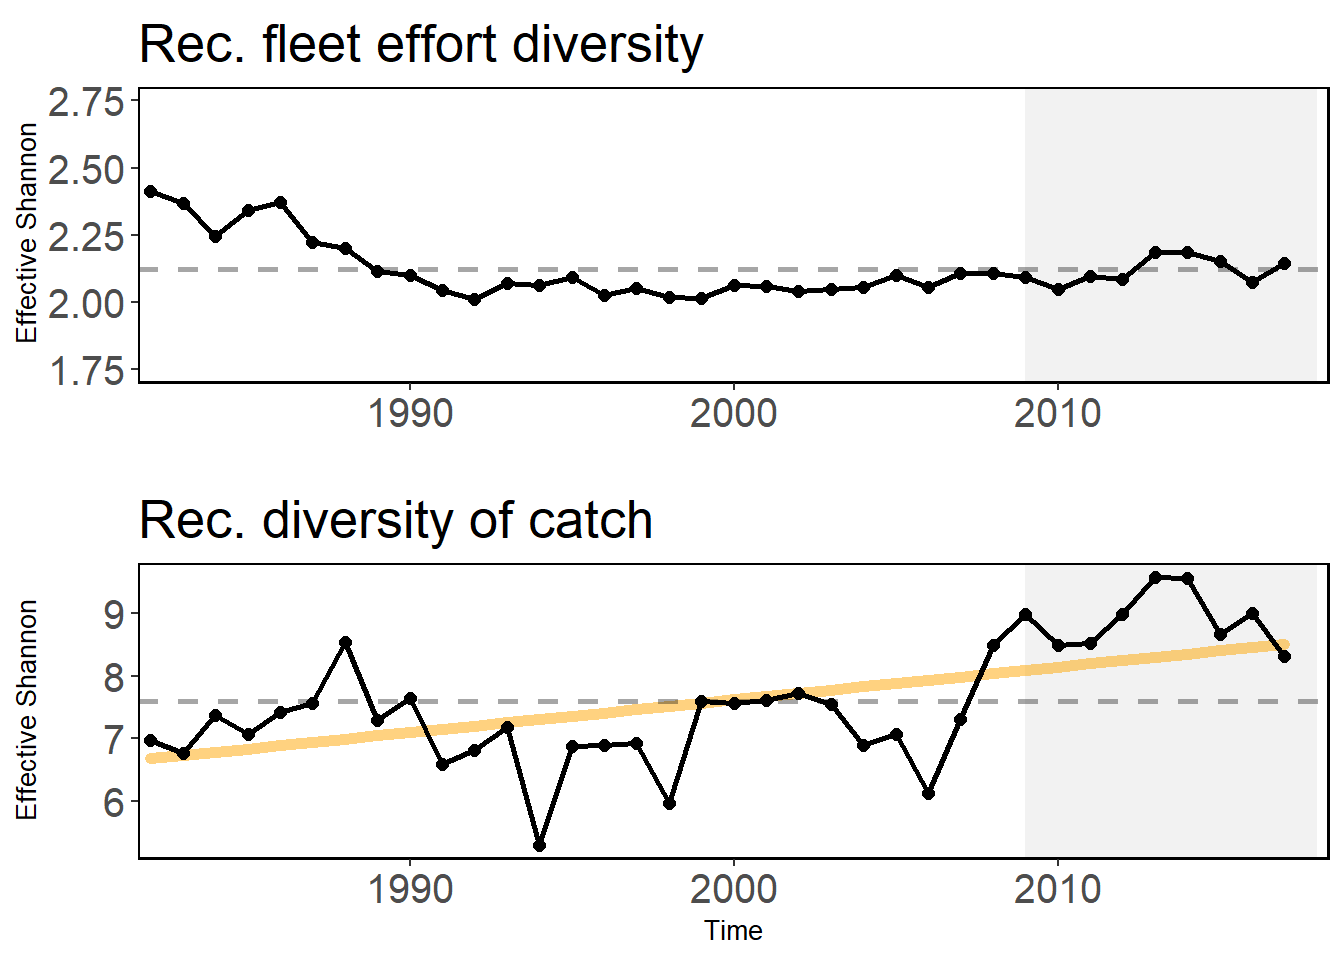
\includegraphics{C:/Users/kimberly.bastille/Desktop/tech-doc/imagesunnamed-chunk-49-1.pdf}
\caption{\label{fig:unnamed-chunk-49}Recreational effort diversity and
diversity of recreational catch in New England.}
\end{figure}

\begin{Shaded}
\begin{Highlighting}[]
\NormalTok{landings_rec <-}\StringTok{ }\NormalTok{ecodata}\OperatorTok{::}\NormalTok{recdat }\OperatorTok\StringTok{ }
\StringTok{  }\KeywordTok{filter}\NormalTok{(EPU }\OperatorTok{==}\StringTok{ "NE"}\NormalTok{,}
\NormalTok{         Var }\OperatorTok{==}\StringTok{ "Recreational Seafood"}\NormalTok{) }\OperatorTok\StringTok{ }
\StringTok{  }\KeywordTok{mutate}\NormalTok{(}\DataTypeTok{hline =} \KeywordTok{mean}\NormalTok{(Value))}

\NormalTok{series.col <-}\StringTok{ "black"}

\KeywordTok{ggplot}\NormalTok{(}\DataTypeTok{data =}\NormalTok{ landings_rec)}\OperatorTok{+}
\StringTok{  }
\StringTok{  }\CommentTok{#Highlight last ten years}
\StringTok{  }\KeywordTok{annotate}\NormalTok{(}\StringTok{"rect"}\NormalTok{, }\DataTypeTok{fill =}\NormalTok{ shade.fill, }\DataTypeTok{alpha =}\NormalTok{ shade.alpha,}
      \DataTypeTok{xmin =}\NormalTok{ x.shade.min , }\DataTypeTok{xmax =}\NormalTok{ x.shade.max,}
      \DataTypeTok{ymin =} \OperatorTok{-}\OtherTok{Inf}\NormalTok{, }\DataTypeTok{ymax =} \OtherTok{Inf}\NormalTok{) }\OperatorTok{+}
\StringTok{  }\KeywordTok{geom_gls}\NormalTok{(}\KeywordTok{aes}\NormalTok{(}\DataTypeTok{x =}\NormalTok{ Time, }\DataTypeTok{y =}\NormalTok{ Value,}
               \DataTypeTok{group =}\NormalTok{ Var),}
             \DataTypeTok{alpha =}\NormalTok{ trend.alpha, }\DataTypeTok{size =}\NormalTok{ trend.size) }\OperatorTok{+}
\StringTok{  }\KeywordTok{geom_line}\NormalTok{(}\KeywordTok{aes}\NormalTok{(}\DataTypeTok{x =}\NormalTok{ Time, }\DataTypeTok{y =}\NormalTok{ Value, }\DataTypeTok{color =}\NormalTok{ Var), }\DataTypeTok{size =}\NormalTok{ lwd) }\OperatorTok{+}
\StringTok{  }\KeywordTok{geom_point}\NormalTok{(}\KeywordTok{aes}\NormalTok{(}\DataTypeTok{x =}\NormalTok{ Time, }\DataTypeTok{y =}\NormalTok{ Value, }\DataTypeTok{color =}\NormalTok{ Var), }\DataTypeTok{size =}\NormalTok{ pcex) }\OperatorTok{+}
\StringTok{  }\KeywordTok{ggtitle}\NormalTok{(}\StringTok{"NE Recreational seafood harvest"}\NormalTok{)}\OperatorTok{+}
\StringTok{  }\KeywordTok{scale_y_continuous}\NormalTok{(}\DataTypeTok{labels =} \ControlFlowTok{function}\NormalTok{(l)\{trans =}\StringTok{ }\NormalTok{l }\OperatorTok{/}\StringTok{ }\DecValTok{1000000}\NormalTok{\})}\OperatorTok{+}
\StringTok{  }\KeywordTok{scale_x_continuous}\NormalTok{(}\DataTypeTok{breaks =} \KeywordTok{seq}\NormalTok{(}\DecValTok{1985}\NormalTok{, }\DecValTok{2015}\NormalTok{, }\DataTypeTok{by =} \DecValTok{5}\NormalTok{), }\DataTypeTok{expand =} \KeywordTok{c}\NormalTok{(}\FloatTok{0.01}\NormalTok{, }\FloatTok{0.01}\NormalTok{)) }\OperatorTok{+}
\StringTok{  }\KeywordTok{scale_color_manual}\NormalTok{(}\DataTypeTok{values =}\NormalTok{ series.col, }\DataTypeTok{aesthetics =} \StringTok{"color"}\NormalTok{)}\OperatorTok{+}
\StringTok{  }\KeywordTok{guides}\NormalTok{(}\DataTypeTok{color =} \OtherTok{FALSE}\NormalTok{) }\OperatorTok{+}
\StringTok{  }\KeywordTok{ylab}\NormalTok{(}\KeywordTok{expression}\NormalTok{(}\StringTok{"Fish caught (10"}\OperatorTok{^}\DecValTok{6}\OperatorTok{*}\StringTok{"n)"}\NormalTok{)) }\OperatorTok{+}

\StringTok{  }\KeywordTok{geom_hline}\NormalTok{(}\KeywordTok{aes}\NormalTok{(}\DataTypeTok{yintercept =}\NormalTok{ hline,}
               
               \DataTypeTok{color =}\NormalTok{ Var),}
           \DataTypeTok{size =}\NormalTok{ hline.size,}
           \DataTypeTok{alpha =}\NormalTok{ hline.alpha,}
           \DataTypeTok{linetype =}\NormalTok{ hline.lty) }\OperatorTok{+}
\StringTok{  }\KeywordTok{theme_ts}\NormalTok{()}
\end{Highlighting}
\end{Shaded}

\begin{figure}
\centering
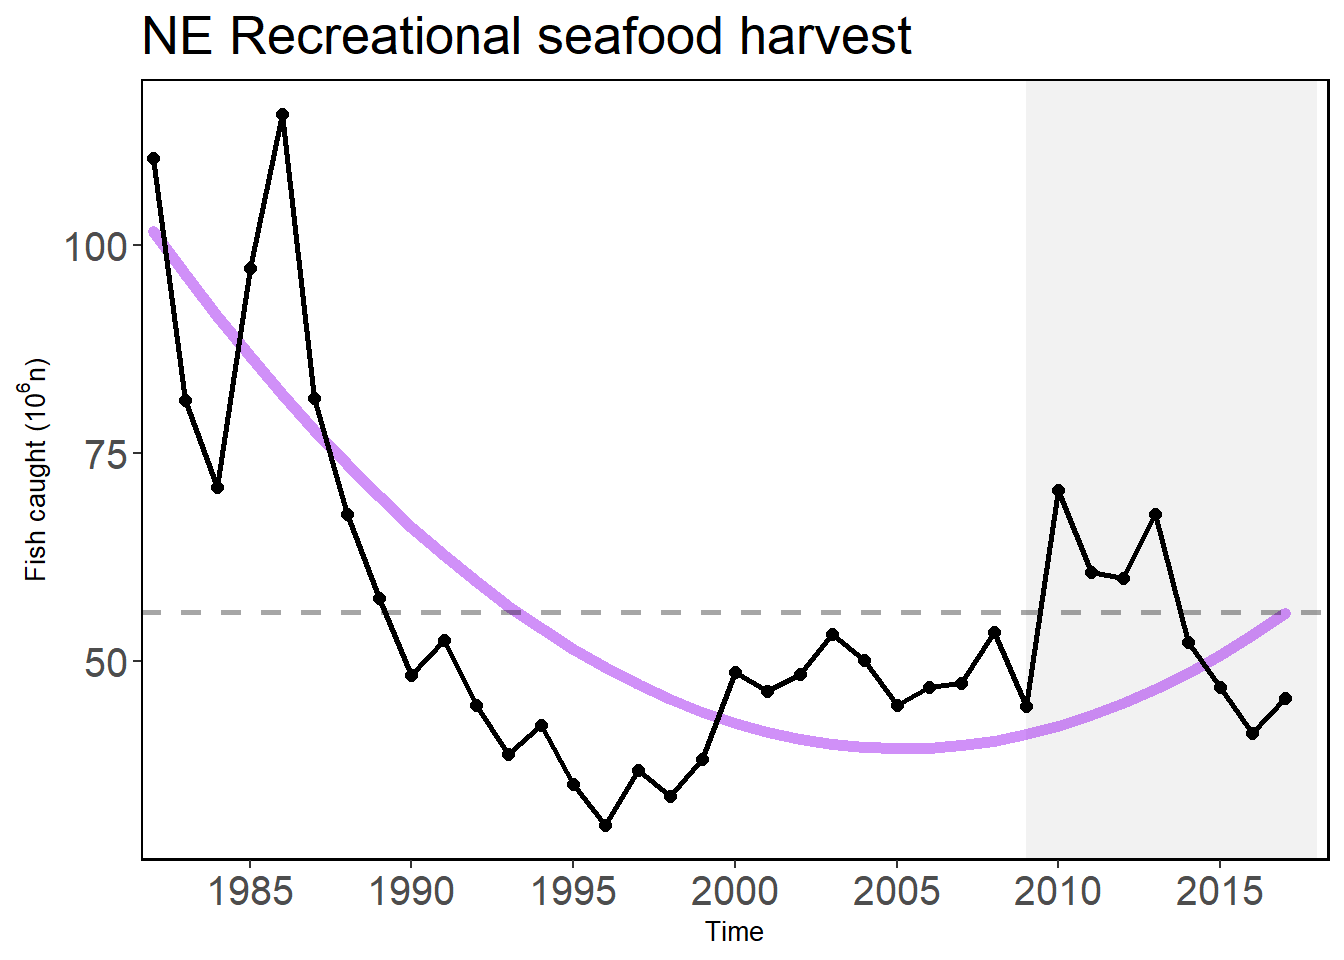
\includegraphics{C:/Users/kimberly.bastille/Desktop/tech-doc/imagesunnamed-chunk-50-1.pdf}
\caption{\label{fig:unnamed-chunk-50}Total recreational seafood harvest in
New England.}
\end{figure}

\begin{Shaded}
\begin{Highlighting}[]
\NormalTok{recdat <-}\StringTok{ }\NormalTok{ecodata}\OperatorTok{::}\NormalTok{recdat }\OperatorTok\StringTok{ }
\StringTok{  }\KeywordTok{filter}\NormalTok{(EPU }\OperatorTok{==}\StringTok{ "NE"}\NormalTok{) }\OperatorTok\StringTok{ }
\StringTok{  }\KeywordTok{group_by}\NormalTok{(Var) }\OperatorTok\StringTok{ }
\StringTok{  }\KeywordTok{mutate}\NormalTok{(}\DataTypeTok{hline =} \KeywordTok{mean}\NormalTok{(Value))}

\NormalTok{ylim_re <-}\StringTok{ }\KeywordTok{c}\NormalTok{(}\FloatTok{5e6}\NormalTok{, }\FloatTok{30e6}\NormalTok{)}
\NormalTok{ylim_rd <-}\StringTok{ }\KeywordTok{c}\NormalTok{(}\FloatTok{1.75}\NormalTok{,}\FloatTok{2.75}\NormalTok{)}
\NormalTok{ylim_ra  <-}\StringTok{ }\KeywordTok{c}\NormalTok{(}\DecValTok{0}\NormalTok{, }\FloatTok{2e6}\NormalTok{)}

\CommentTok{#Create dataframe for label locations}
\CommentTok{# label_loc <- data.frame(xloc = min(recdat$Time)+0.3,}
\CommentTok{#                         yloc = c(ylim_re[2]*0.975,}
\CommentTok{#                                  ylim_rd[2]*0.975,}
\CommentTok{#                                  ylim_ra[2]*0.975),}
\CommentTok{#                         labels = LETTERS[1:3],}
\CommentTok{#                         Var = c("Recreational Effort",}
\CommentTok{#                                 "Recreational fleet effort diversity across modes",}
\CommentTok{#                                 "Recreational anglers"))}

\NormalTok{series.col <-}\StringTok{ "black"}
\CommentTok{#x.shade.min <- max(recdat$Time, na.rm = T) - 9}
\CommentTok{#x.shade.max <- max(recdat$Time, na.rm = T)}

\NormalTok{series.col <-}\StringTok{ "black"}

\NormalTok{rec_effort <-}\StringTok{ }\NormalTok{recdat }\OperatorTok\StringTok{ }
\StringTok{  }\KeywordTok{filter}\NormalTok{(Var }\OperatorTok{==}\StringTok{ "Recreational Effort"}\NormalTok{) }\OperatorTok\StringTok{ }
\StringTok{  }\KeywordTok{ggplot}\NormalTok{() }\OperatorTok{+}\StringTok{ }
\StringTok{ }\CommentTok{#Highlight last ten years}
\StringTok{  }\KeywordTok{annotate}\NormalTok{(}\StringTok{"rect"}\NormalTok{, }\DataTypeTok{fill =}\NormalTok{ shade.fill, }\DataTypeTok{alpha =}\NormalTok{ shade.alpha,}
      \DataTypeTok{xmin =}\NormalTok{ x.shade.min , }\DataTypeTok{xmax =}\NormalTok{ x.shade.max,}
      \DataTypeTok{ymin =} \OperatorTok{-}\OtherTok{Inf}\NormalTok{, }\DataTypeTok{ymax =} \OtherTok{Inf}\NormalTok{) }\OperatorTok{+}
\StringTok{    }\CommentTok{#label}
\StringTok{  }\CommentTok{# annotate("text", }
\StringTok{  }\CommentTok{#          x = label_loc[label_loc$Var == "Recreational Effort",]$xloc,}
\StringTok{  }\CommentTok{#          y = label_loc[label_loc$Var == "Recreational Effort",]$yloc,}
\StringTok{  }\CommentTok{#          label = label_loc[label_loc$Var == "Recreational Effort",]$labels,}
\StringTok{  }\CommentTok{#          size = letter_size)+}
\StringTok{  }\KeywordTok{geom_gls}\NormalTok{(}\KeywordTok{aes}\NormalTok{(}\DataTypeTok{x =}\NormalTok{ Time, }\DataTypeTok{y =}\NormalTok{ Value,}
               \DataTypeTok{group =}\NormalTok{ Var),}
             \DataTypeTok{alpha =}\NormalTok{ trend.alpha, }\DataTypeTok{size =}\NormalTok{ trend.size) }\OperatorTok{+}
\StringTok{  }\KeywordTok{geom_line}\NormalTok{(}\KeywordTok{aes}\NormalTok{(}\DataTypeTok{x =}\NormalTok{ Time, }\DataTypeTok{y =}\NormalTok{ Value, }\DataTypeTok{color =}\NormalTok{ Var), }\DataTypeTok{size =}\NormalTok{ lwd) }\OperatorTok{+}
\StringTok{  }\KeywordTok{geom_point}\NormalTok{(}\KeywordTok{aes}\NormalTok{(}\DataTypeTok{x =}\NormalTok{ Time, }\DataTypeTok{y =}\NormalTok{ Value, }\DataTypeTok{color =}\NormalTok{ Var), }\DataTypeTok{size =}\NormalTok{ pcex) }\OperatorTok{+}

\StringTok{  }\KeywordTok{scale_x_continuous}\NormalTok{(}\DataTypeTok{expand =} \KeywordTok{c}\NormalTok{(}\FloatTok{0.01}\NormalTok{, }\FloatTok{0.01}\NormalTok{)) }\OperatorTok{+}
\StringTok{  }\KeywordTok{scale_y_continuous}\NormalTok{(}\DataTypeTok{labels =} \ControlFlowTok{function}\NormalTok{(l)\{trans =}\StringTok{ }\NormalTok{l }\OperatorTok{/}\StringTok{ }\DecValTok{1000000}\NormalTok{\}, }\DataTypeTok{limits =}\NormalTok{ ylim_re)}\OperatorTok{+}
\StringTok{  }\KeywordTok{scale_color_manual}\NormalTok{(}\DataTypeTok{values =}\NormalTok{ series.col, }\DataTypeTok{aesthetics =} \StringTok{"color"}\NormalTok{)}\OperatorTok{+}
\StringTok{  }\KeywordTok{guides}\NormalTok{(}\DataTypeTok{color =} \OtherTok{FALSE}\NormalTok{) }\OperatorTok{+}
\StringTok{  }\KeywordTok{ggtitle}\NormalTok{(}\StringTok{"Recreational effort"}\NormalTok{) }\OperatorTok{+}
\StringTok{  }\KeywordTok{ylab}\NormalTok{(}\KeywordTok{expression}\NormalTok{(}\StringTok{"Days fished (10"}\OperatorTok{^}\DecValTok{6}\OperatorTok{*}\StringTok{" days)"}\NormalTok{)) }\OperatorTok{+}
\StringTok{  }\KeywordTok{xlab}\NormalTok{(}\StringTok{""}\NormalTok{)}\OperatorTok{+}
\StringTok{  }\KeywordTok{geom_hline}\NormalTok{(}\KeywordTok{aes}\NormalTok{(}\DataTypeTok{yintercept =}\NormalTok{ hline,}
               \DataTypeTok{color =}\NormalTok{ Var),}
           \DataTypeTok{size =}\NormalTok{ hline.size,}
           \DataTypeTok{alpha =}\NormalTok{ hline.alpha,}
           \DataTypeTok{linetype =}\NormalTok{ hline.lty) }\OperatorTok{+}
\StringTok{  }\KeywordTok{theme_ts}\NormalTok{() }


\NormalTok{rec_anglers <-}\StringTok{ }\NormalTok{recdat }\OperatorTok\StringTok{ }
\StringTok{  }\KeywordTok{filter}\NormalTok{(Var }\OperatorTok{==}\StringTok{ "Recreational anglers"}\NormalTok{) }\OperatorTok\StringTok{ }
\StringTok{  }\KeywordTok{ggplot}\NormalTok{() }\OperatorTok{+}\StringTok{ }
\StringTok{ }\CommentTok{#Highlight last ten years}
\StringTok{  }\KeywordTok{annotate}\NormalTok{(}\StringTok{"rect"}\NormalTok{, }\DataTypeTok{fill =}\NormalTok{ shade.fill, }\DataTypeTok{alpha =}\NormalTok{ shade.alpha,}
      \DataTypeTok{xmin =}\NormalTok{ x.shade.min , }\DataTypeTok{xmax =}\NormalTok{ x.shade.max,}
      \DataTypeTok{ymin =} \OperatorTok{-}\OtherTok{Inf}\NormalTok{, }\DataTypeTok{ymax =} \OtherTok{Inf}\NormalTok{) }\OperatorTok{+}
\StringTok{    }\CommentTok{# annotate("text", }
\StringTok{    }\CommentTok{#        x = label_loc[label_loc$Var == "Recreational anglers",]$xloc,}
\StringTok{    }\CommentTok{#        y = label_loc[label_loc$Var == "Recreational anglers",]$yloc,}
\StringTok{    }\CommentTok{#        label = label_loc[label_loc$Var == "Recreational anglers",]$labels,}
\StringTok{    }\CommentTok{#        size = letter_size)+}
\StringTok{  }\KeywordTok{geom_gls}\NormalTok{(}\KeywordTok{aes}\NormalTok{(}\DataTypeTok{x =}\NormalTok{ Time, }\DataTypeTok{y =}\NormalTok{ Value,}
               \DataTypeTok{group =}\NormalTok{ Var),}
             \DataTypeTok{alpha =}\NormalTok{ trend.alpha, }\DataTypeTok{size =}\NormalTok{ trend.size) }\OperatorTok{+}
\StringTok{  }\KeywordTok{geom_line}\NormalTok{(}\KeywordTok{aes}\NormalTok{(}\DataTypeTok{x =}\NormalTok{ Time, }\DataTypeTok{y =}\NormalTok{ Value, }\DataTypeTok{color =}\NormalTok{ Var), }\DataTypeTok{size =}\NormalTok{ lwd) }\OperatorTok{+}
\StringTok{  }\KeywordTok{geom_point}\NormalTok{(}\KeywordTok{aes}\NormalTok{(}\DataTypeTok{x =}\NormalTok{ Time, }\DataTypeTok{y =}\NormalTok{ Value, }\DataTypeTok{color =}\NormalTok{ Var), }\DataTypeTok{size =}\NormalTok{ pcex) }\OperatorTok{+}

\StringTok{  }\KeywordTok{scale_x_continuous}\NormalTok{(}\DataTypeTok{expand =} \KeywordTok{c}\NormalTok{(}\FloatTok{0.01}\NormalTok{, }\FloatTok{0.01}\NormalTok{)) }\OperatorTok{+}
\StringTok{  }\KeywordTok{scale_y_continuous}\NormalTok{(}\DataTypeTok{labels =} \ControlFlowTok{function}\NormalTok{(l)\{trans =}\StringTok{ }\NormalTok{l }\OperatorTok{/}\StringTok{ }\DecValTok{1000000}\NormalTok{\}, }\DataTypeTok{limits =}\NormalTok{ ylim_ra)}\OperatorTok{+}
\StringTok{  }\KeywordTok{scale_color_manual}\NormalTok{(}\DataTypeTok{values =}\NormalTok{ series.col, }\DataTypeTok{aesthetics =} \StringTok{"color"}\NormalTok{)}\OperatorTok{+}
\StringTok{  }\KeywordTok{guides}\NormalTok{(}\DataTypeTok{color =} \OtherTok{FALSE}\NormalTok{) }\OperatorTok{+}
\StringTok{  }\KeywordTok{ggtitle}\NormalTok{(}\StringTok{"Recreational anglers"}\NormalTok{)}\OperatorTok{+}
\StringTok{  }\KeywordTok{ylab}\NormalTok{(}\KeywordTok{expression}\NormalTok{(}\StringTok{"Anglers (10"}\OperatorTok{^}\DecValTok{6}\OperatorTok{*}\StringTok{" n)"}\NormalTok{)) }\OperatorTok{+}
\StringTok{  }\KeywordTok{xlab}\NormalTok{(}\StringTok{"Time"}\NormalTok{)}\OperatorTok{+}
\StringTok{  }\KeywordTok{geom_hline}\NormalTok{(}\KeywordTok{aes}\NormalTok{(}\DataTypeTok{yintercept =}\NormalTok{ hline,}
               \DataTypeTok{color =}\NormalTok{ Var),}
           \DataTypeTok{size =}\NormalTok{ hline.size,}
           \DataTypeTok{alpha =}\NormalTok{ hline.alpha,}
           \DataTypeTok{linetype =}\NormalTok{ hline.lty) }\OperatorTok{+}
\StringTok{  }\KeywordTok{theme_ts}\NormalTok{()}

\NormalTok{cowplot}\OperatorTok{::}\KeywordTok{plot_grid}\NormalTok{(rec_effort, }
                   \CommentTok{#rec_div, }
\NormalTok{                   rec_anglers, }
                   \CommentTok{#rec_div_catch,}
                   \DataTypeTok{ncol =} \DecValTok{1}\NormalTok{, }
                   \DataTypeTok{align =} \StringTok{"hv"}\NormalTok{) }\OperatorTok{+}
\StringTok{    }\KeywordTok{theme}\NormalTok{(}\DataTypeTok{plot.margin =} \KeywordTok{unit}\NormalTok{(}\KeywordTok{c}\NormalTok{(}\FloatTok{0.1}\NormalTok{, }\DecValTok{0}\NormalTok{, }\DecValTok{0}\NormalTok{, }\DecValTok{0}\NormalTok{), }\StringTok{"cm"}\NormalTok{))}
\end{Highlighting}
\end{Shaded}

\begin{figure}
\centering
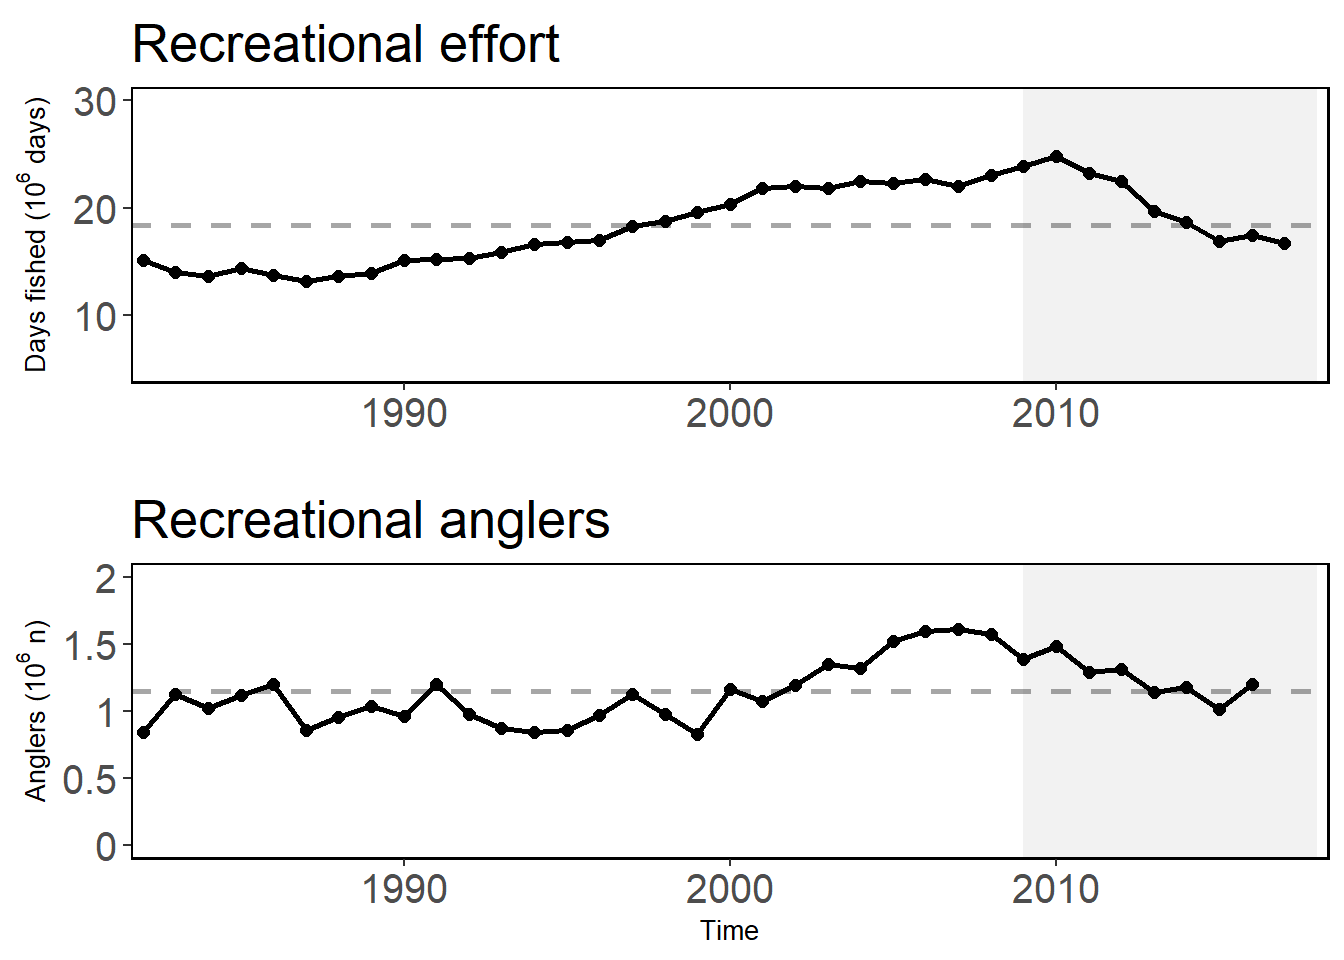
\includegraphics{C:/Users/kimberly.bastille/Desktop/tech-doc/imagesunnamed-chunk-51-1.pdf}
\caption{\label{fig:unnamed-chunk-51}Recreational effort and number of
recreational anglers in New England.}
\end{figure}

\chapter{Right Whale Abundance}\label{right-whale-abundance}

\textbf{Description}: Right Whale

\textbf{Found in}: State of the Ecosystem - Gulf of Maine \& Georges
Bank (2017, 2018, 2019), State of the Ecosystem - Mid-Atlantic (2017,
2018, 2019)

\textbf{Indicator category}: Synthesis of published information;
Published methods

\textbf{Contributor(s)}: Christopher D. Orphanides

\textbf{Data steward}: Chris Orphanides,
\href{mailto:chris.orphanides@noaa.gov}{\nolinkurl{chris.orphanides@noaa.gov}}

\textbf{Point of contact}: Richard Pace,
\href{mailto:richard.pace@noaa.gov}{\nolinkurl{richard.pace@noaa.gov}}

\textbf{Public availability statement}: Source data are available from
the New England Aquarium upon request. Derived data are available
\href{http://comet.nefsc.noaa.gov/erddap/tabledap/protected_species_soe_v1.html}{here}

\section{Methods}\label{methods-23}

\subsection{Data sources}\label{data-sources-23}

The North Atlantic right whale abundance estimates were taken from a
published document (see Pace, Corkeron, and Kraus
\protect\hyperlink{ref-Pace2017}{2017}), except for the most recent 2016
and 2017 estimates. Abundance estimates from 2016 and 2017 were taken
from the 2016 NOAA marine mammal stock assessment (Hayes et al.
\protect\hyperlink{ref-Hayes2017}{2017}) and an unpublished 2017 stock
assessment.

\subsection{Data extraction}\label{data-extraction-19}

Data were collected from existing reports and validated by report
authors.

\subsection{Data analysis}\label{data-analysis-21}

Analysis for right whale abundance estimates is provided by Pace,
Corkeron, and Kraus (\protect\hyperlink{ref-Pace2017}{2017}), and code
can be found in the
\href{https://onlinelibrary.wiley.com/action/downloadSupplement?doi=10.1002\%2Fece3.3406\&file=ece33406-sup-0001-SupInfo.docx}{supplemental
materials}.

\subsection{Data processing}\label{data-processing-14}

Time series of right whale abundance estimates were formatted for
inclusion in the ecodata R package using the following R code.

\begin{Shaded}
\begin{Highlighting}[]
\CommentTok{#Processing for North Atlantic Right Whale data}

\CommentTok{#See full documentation for these data at https://noaa-edab.github.io/tech-doc/right-whale-abundance.html}

\KeywordTok{library}\NormalTok{(dplyr)}
\KeywordTok{library}\NormalTok{(tidyr)}
\KeywordTok{library}\NormalTok{(stringr)}

\NormalTok{raw.dir <-}\StringTok{ }\NormalTok{here}\OperatorTok{::}\KeywordTok{here}\NormalTok{(}\StringTok{"data-raw"}\NormalTok{)}

\NormalTok{get_narw <-}\StringTok{ }\ControlFlowTok{function}\NormalTok{(}\DataTypeTok{save_clean =}\NormalTok{ F)\{}
\NormalTok{  narw <-}\StringTok{ }\KeywordTok{read.csv}\NormalTok{(}\KeywordTok{file.path}\NormalTok{(raw.dir, }\StringTok{"narw_numbers.csv"}\NormalTok{)) }\OperatorTok\StringTok{ }
\StringTok{    }\KeywordTok{gather}\NormalTok{(.,Var,Value,}\OperatorTok{-}\NormalTok{YEAR) }\OperatorTok\StringTok{ }
\StringTok{    }\KeywordTok{mutate}\NormalTok{(}\DataTypeTok{Var =} \KeywordTok{tolower}\NormalTok{(}\KeywordTok{paste}\NormalTok{(}\StringTok{"right whale abundance"}\NormalTok{,Var)),}
           \DataTypeTok{Units =}  \StringTok{"n"}\NormalTok{,}
           \DataTypeTok{EPU =} \StringTok{"All"}\NormalTok{) }\OperatorTok\StringTok{ }
\StringTok{    }\KeywordTok{mutate}\NormalTok{(}\DataTypeTok{Var =} \KeywordTok{ifelse}\NormalTok{(}\KeywordTok{str_detect}\NormalTok{(Var, }\StringTok{"median"}\NormalTok{),}
                        \StringTok{"right whale abundance median"}\NormalTok{,}
                        \KeywordTok{ifelse}\NormalTok{(}\KeywordTok{str_detect}\NormalTok{(Var, }\StringTok{"lcl"}\NormalTok{),}
                               \StringTok{"right whale abundance lcl"}\NormalTok{,}
                               \StringTok{"right whale abundance ucl"}\NormalTok{))) }\OperatorTok\StringTok{ }
\StringTok{    }\NormalTok{dplyr}\OperatorTok{::}\KeywordTok{rename}\NormalTok{(}\DataTypeTok{Time =}\NormalTok{ YEAR)}
  
  \ControlFlowTok{if}\NormalTok{ (save_clean)\{}
\NormalTok{    usethis}\OperatorTok{::}\KeywordTok{use_data}\NormalTok{(narw, }\DataTypeTok{overwrite =}\NormalTok{ T)}
\NormalTok{  \} }\ControlFlowTok{else}\NormalTok{ \{}
    \KeywordTok{return}\NormalTok{(narw)}
\NormalTok{  \}}
  
\NormalTok{\}}
\end{Highlighting}
\end{Shaded}

\subsection{Plotting}\label{plotting-16}

\begin{Shaded}
\begin{Highlighting}[]
\CommentTok{# Relative working directories}
\NormalTok{data.dir  <-}\StringTok{ }\NormalTok{here}\OperatorTok{::}\KeywordTok{here}\NormalTok{(}\StringTok{'data'}\NormalTok{)}
\NormalTok{r.dir <-}\StringTok{ }\NormalTok{here}\OperatorTok{::}\KeywordTok{here}\NormalTok{(}\StringTok{'R'}\NormalTok{)}

\CommentTok{# Load data}
\KeywordTok{load}\NormalTok{(}\KeywordTok{file.path}\NormalTok{(data.dir,}\StringTok{"SOE_data_erddap.Rdata"}\NormalTok{))}

\CommentTok{# Source plotting functions}
\KeywordTok{source}\NormalTok{(}\KeywordTok{file.path}\NormalTok{(r.dir,}\StringTok{"BasePlot_source.R"}\NormalTok{))}

\KeywordTok{par}\NormalTok{(}\DataTypeTok{mar =} \KeywordTok{c}\NormalTok{(}\DecValTok{5}\NormalTok{,}\DecValTok{5}\NormalTok{,}\DecValTok{4}\NormalTok{,}\DecValTok{1}\NormalTok{))}
\KeywordTok{soe.plot}\NormalTok{(SOE.data, }\StringTok{'Time'}\NormalTok{, }\StringTok{"right_whale_median"}\NormalTok{, }\DataTypeTok{rel.y.num =} \FloatTok{1.2}\NormalTok{, }
         \DataTypeTok{full.trend =}\NormalTok{ F, }\DataTypeTok{lwd =} \FloatTok{1.5}\NormalTok{, }\DataTypeTok{point.cex =} \DecValTok{1}\NormalTok{, }\DataTypeTok{end.start =} \DecValTok{2007}\NormalTok{,}
         \DataTypeTok{x.label =} \StringTok{'Year'}\NormalTok{, }\DataTypeTok{y.label =} \StringTok{'Abundance, n'}\NormalTok{, }
         \DataTypeTok{rel.y.text =} \DecValTok{1}\NormalTok{)}

\NormalTok{lw_CI <-}\StringTok{ }\NormalTok{SOE.data[Var }\OperatorTok{==}\StringTok{ 'right_whale_lower_95'}\NormalTok{, }\KeywordTok{list}\NormalTok{(Time, Value)]}
\NormalTok{up_CI <-}\StringTok{ }\NormalTok{SOE.data[Var }\OperatorTok{==}\StringTok{ 'right_whale_upper_95'}\NormalTok{, }\KeywordTok{list}\NormalTok{(Time, Value)]}
\KeywordTok{points}\NormalTok{(lw_CI, }\DataTypeTok{type  =} \StringTok{"l"}\NormalTok{, }\DataTypeTok{lty =} \DecValTok{2}\NormalTok{, }\DataTypeTok{col =} \KeywordTok{adjustcolor}\NormalTok{(}\StringTok{"darkorange"}\NormalTok{, .}\DecValTok{6}\NormalTok{), }\DataTypeTok{lwd =} \FloatTok{2.5}\NormalTok{)}
\KeywordTok{points}\NormalTok{(up_CI, }\DataTypeTok{type  =} \StringTok{"l"}\NormalTok{, }\DataTypeTok{lty =} \DecValTok{2}\NormalTok{, }\DataTypeTok{col =} \KeywordTok{adjustcolor}\NormalTok{(}\StringTok{"darkorange"}\NormalTok{, .}\DecValTok{6}\NormalTok{), }\DataTypeTok{lwd =} \FloatTok{2.5}\NormalTok{)}
\end{Highlighting}
\end{Shaded}

\begin{figure}
\centering
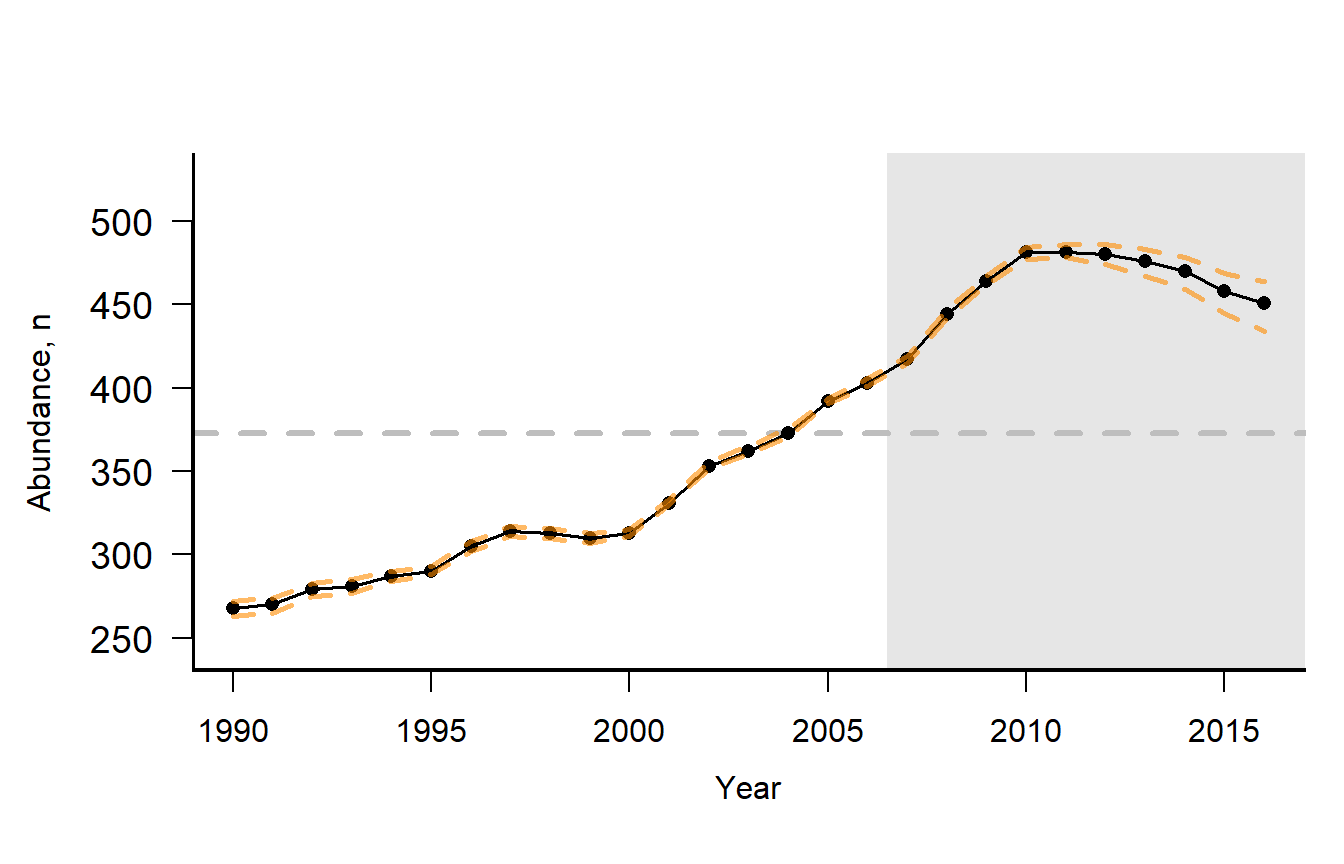
\includegraphics{C:/Users/kimberly.bastille/Desktop/tech-doc/imagesrw-abundance-1.pdf}
\caption{\label{fig:rw-abundance}North Atlantic right whale population
estimates shown with 95\% credible intervals.}
\end{figure}

\chapter{Seabird diet and
productivity}\label{seabird-diet-and-productivity}

\textbf{Description}: Common tern annual diet and productivity at seven
Gulf of Maine colonies managed by the National Audubon Society's Seabird
Restoration Program

\textbf{Indicator category}: Published method

\textbf{Found in}: State of the Ecosystem - New England (2019)

\textbf{Contributor(s)}: Don Lyons, Steve Kress, Paula Shannon, Sue
Schubel

\textbf{Data steward}: Don Lyons,
\href{mailto:dlyons@audubon.org}{\nolinkurl{dlyons@audubon.org}}

\textbf{Point of contact}: Don Lyons,
\href{mailto:dlyons@audubon.org}{\nolinkurl{dlyons@audubon.org}}

\textbf{Public availability statement}: Please email
\href{mailto:dlyons@audubon.org}{\nolinkurl{dlyons@audubon.org}} for
further information and queries on this indicator source data.

\section{Methods}\label{methods-24}

\textbf{Chick diet}

Common tern (\emph{Sterna hirundo}) chick diet was quantified at each of
the seven nesting sites (Fig. \ref{fig:map-and-prey}a) by observing
chick provisioning from portable observation blinds. The locations of
observation blinds within each site were chosen to maximize the number
of visible nests, and provisioning observations took place between
mid-June and early August annually. Observations of chick diet were made
during one or two, three to four hour periods throughout the day, but
typically proceed according to nest activity levels (moreso in the
morning hours). Observations began with chicks as soon as they hatched,
and continue until the chicks fledged or died.

Most common tern prey species were identifiable to the species level due
to distinct size, color and shape. However, when identification was not
possible or was unclear, prey species were listed as ``unknown'' or
``unknown fish''. More detailed methods can be found in Hall, Kress, and
Griffin (\protect\hyperlink{ref-hall2000}{2000}).

\textbf{Nest productivity}

Common tern nest productivity, in terms of the number of fledged chicks
per nest, was collected annually from fenced enclosures at island
nesting sites (known as ``productivity plots''). Newly hatched chicks
within these enclosures were weighed, marked or banded, and observed
until fledging, death, or until a 15 day period had passed when chicks
were assumed to have fledged. Productivity was also quantified from
observer blinds for nests outside of the productivity plots where chicks
were marked for identification. More detailed methods for quantifying
nest productivity can be found in Hall and Kress
(\protect\hyperlink{ref-hall2004}{2004})

\subsection{Data sources}\label{data-sources-24}

Common tern diet and nest productivity data were provided by the
National Audubon Society's Seabird Restoration Program.

\subsection{Data processing}\label{data-processing-15}

Diet and productivity data were formatted for inclusion in the ecodata R
package using the following R code.

\begin{Shaded}
\begin{Highlighting}[]
\CommentTok{# Process raw common tern productivity and diet data}

\CommentTok{# If save == TRUE, processed data are saved as a .Rds file to the data directory. }

\CommentTok{# Function returns a processed data frame containing time series of productivity and diet}
\CommentTok{# composition for common tern at different islands in southern Gulf of Maine. The first three letters}
\CommentTok{# in the variable "Var" correspond to the island at which sampling occurred, with COTE referring to }
\CommentTok{# Common Tern. If "Var" includes productivity, then "Value" is the average number of fledged chicks.}
\CommentTok{# Otherwise, if "Var" specifies diet, then  "Value"  is equal to the count of observed prey type. }
\CommentTok{# For example, "EER COTE Diet Amphipod" refers to the number of preyed upon amphipods observed at Eastern}
\CommentTok{# Egg Rock in a given year. }

\KeywordTok{library}\NormalTok{(dplyr)}
\KeywordTok{library}\NormalTok{(tidyr)}

\CommentTok{#Get raw data}
\NormalTok{raw.dir <-}\StringTok{ }\NormalTok{here}\OperatorTok{::}\KeywordTok{here}\NormalTok{(}\StringTok{"data-raw"}\NormalTok{)}


\NormalTok{get_commontern <-}\StringTok{ }\ControlFlowTok{function}\NormalTok{(}\DataTypeTok{save_clean =}\NormalTok{ F)\{}

\NormalTok{  d <-}\StringTok{ }\KeywordTok{read.csv}\NormalTok{(}\KeywordTok{file.path}\NormalTok{(raw.dir,}\StringTok{"Audubon SRP Common Tern Data.csv"}\NormalTok{))}
  
  \CommentTok{#Process}
\NormalTok{  common_tern <-}\StringTok{ }\NormalTok{d }\OperatorTok
\StringTok{    }\KeywordTok{filter}\NormalTok{(Island }\OperatorTok{!=}\StringTok{ ""}\NormalTok{) }\OperatorTok\StringTok{ }
\StringTok{    }\NormalTok{tidyr}\OperatorTok{::}\KeywordTok{gather}\NormalTok{(., Var, Value, }\OperatorTok{-}\NormalTok{Year, }\OperatorTok{-}\NormalTok{Species, }\OperatorTok{-}\NormalTok{Island) }\OperatorTok
\StringTok{    }\KeywordTok{mutate}\NormalTok{(}\DataTypeTok{Species =} \KeywordTok{ifelse}\NormalTok{(Var }\OperatorTok{!=}\StringTok{ "Productivity"}\NormalTok{,}
                                   \KeywordTok{paste}\NormalTok{(Species, }\StringTok{"Diet"}\NormalTok{), }\StringTok{"COTE"}\NormalTok{)) }\OperatorTok\StringTok{ }
\StringTok{    }\KeywordTok{unite}\NormalTok{(., }\StringTok{"Var"}\NormalTok{, }\KeywordTok{c}\NormalTok{(}\StringTok{"Island"}\NormalTok{, }\StringTok{"Species"}\NormalTok{, }\StringTok{"Var"}\NormalTok{), }\DataTypeTok{sep =} \StringTok{" "}\NormalTok{) }\OperatorTok\StringTok{ }
\StringTok{    }\NormalTok{dplyr}\OperatorTok{::}\KeywordTok{rename}\NormalTok{(}\DataTypeTok{Time =}\NormalTok{ Year) }\OperatorTok\StringTok{ }
\StringTok{    }\KeywordTok{mutate}\NormalTok{(}\DataTypeTok{EPU =} \StringTok{"GOM"}\NormalTok{,}
                  \DataTypeTok{Units =} \KeywordTok{ifelse}\NormalTok{(stringr}\OperatorTok{::}\KeywordTok{str_detect}\NormalTok{(Var, }\StringTok{"Productivity"}\NormalTok{),}
                                 \StringTok{"fledged chicks per nest"}\NormalTok{,}\StringTok{"N"}\NormalTok{)) }
  
  \ControlFlowTok{if}\NormalTok{ (save_clean)\{}

\NormalTok{    usethis}\OperatorTok{::}\KeywordTok{use_data}\NormalTok{(common_tern, }\DataTypeTok{overwrite =}\NormalTok{ T)}
\NormalTok{  \} }\ControlFlowTok{else}\NormalTok{ \{}
    \KeywordTok{return}\NormalTok{(common_tern)}
\NormalTok{  \}}
\NormalTok{\}}
\end{Highlighting}
\end{Shaded}

\subsection{Data analysis}\label{data-analysis-22}

Raw diet data were used to create time series of mean shannon diversity
through time and across study sites using the \texttt{vegan} R package
(Oksanen et al. \protect\hyperlink{ref-R-vegan}{2019}). Diet diversity
is presented along with nest productivity (+/- 1 SE) below.

\begin{Shaded}
\begin{Highlighting}[]
\CommentTok{#Calculating time series of diversity indices using the vegan package. }
\NormalTok{diet_div <-}\StringTok{ }\NormalTok{ecodata}\OperatorTok{::}\NormalTok{common_tern }\OperatorTok\StringTok{ }
\StringTok{  }\KeywordTok{filter}\NormalTok{(}\KeywordTok{str_detect}\NormalTok{(Var, }\StringTok{"Diet"}\NormalTok{),}
         \OperatorTok{!}\KeywordTok{str_detect}\NormalTok{(Var, }\StringTok{"Sum"}\NormalTok{)) }\OperatorTok\StringTok{ }
\StringTok{  }\KeywordTok{mutate}\NormalTok{(}\DataTypeTok{Island =} \KeywordTok{word}\NormalTok{(Var, }\DecValTok{1}\NormalTok{),}
         \DataTypeTok{Var =} \KeywordTok{word}\NormalTok{(Var, }\DecValTok{4}\NormalTok{)) }\OperatorTok\StringTok{ }
\StringTok{  }\KeywordTok{group_by}\NormalTok{(Island, Time) }\OperatorTok
\StringTok{  }\NormalTok{dplyr}\OperatorTok{::}\KeywordTok{summarise}\NormalTok{(}\DataTypeTok{evenness =} \KeywordTok{diversity}\NormalTok{(Value)}\OperatorTok{/}\KeywordTok{log}\NormalTok{(}\KeywordTok{specnumber}\NormalTok{(Value)),}
                   \DataTypeTok{shannon =} \KeywordTok{diversity}\NormalTok{(Value),}
                   \DataTypeTok{simpson =} \KeywordTok{diversity}\NormalTok{(Value, }\DataTypeTok{index =} \StringTok{"simpson"}\NormalTok{)) }\OperatorTok\StringTok{ }
\StringTok{  }\KeywordTok{gather}\NormalTok{(.,Var,Value,}\OperatorTok{-}\NormalTok{Island, }\OperatorTok{-}\NormalTok{Time) }\OperatorTok\StringTok{ }
\StringTok{  }\KeywordTok{group_by}\NormalTok{(Var, Time) }\OperatorTok
\StringTok{  }\NormalTok{dplyr}\OperatorTok{::}\KeywordTok{summarize}\NormalTok{(}\DataTypeTok{Value =} \KeywordTok{mean}\NormalTok{(Value, }\DataTypeTok{na.rm =}\NormalTok{ T),}
                   \DataTypeTok{sd =} \KeywordTok{sd}\NormalTok{(Value, }\DataTypeTok{na.rm =}\NormalTok{ T),}
                   \DataTypeTok{n =} \KeywordTok{n}\NormalTok{()) }\OperatorTok
\StringTok{  }\KeywordTok{group_by}\NormalTok{(Var) }\OperatorTok\StringTok{ }
\StringTok{  }\KeywordTok{mutate}\NormalTok{(}\DataTypeTok{hline =} \KeywordTok{mean}\NormalTok{(Value, }\DataTypeTok{na.rm =}\NormalTok{ T))}
\end{Highlighting}
\end{Shaded}

\begin{Shaded}
\begin{Highlighting}[]
\NormalTok{aggregate_prod <-}\StringTok{ }\NormalTok{ecodata}\OperatorTok{::}\NormalTok{common_tern }\OperatorTok\StringTok{ }
\StringTok{    }\KeywordTok{filter}\NormalTok{(}\OperatorTok{!}\KeywordTok{str_detect}\NormalTok{(Var, }\StringTok{"Diet|Sum"}\NormalTok{))  }\OperatorTok\StringTok{ }
\StringTok{  }\KeywordTok{mutate}\NormalTok{(}\DataTypeTok{Island =} \KeywordTok{word}\NormalTok{(Var, }\DecValTok{1}\NormalTok{),}
         \DataTypeTok{Var =} \KeywordTok{word}\NormalTok{(Var, }\DecValTok{3}\NormalTok{),}
         \DataTypeTok{Island =}\NormalTok{ plyr}\OperatorTok{::}\KeywordTok{mapvalues}\NormalTok{(Island, }\DataTypeTok{from =} \KeywordTok{c}\NormalTok{(}\StringTok{"EER"}\NormalTok{,}\StringTok{"JI"}\NormalTok{,}\StringTok{"MR"}\NormalTok{,}\StringTok{"OGI"}\NormalTok{,}\StringTok{"PINWR"}\NormalTok{,}\StringTok{"SINWR"}\NormalTok{,}\StringTok{"STI"}\NormalTok{),}
                                  \DataTypeTok{to =} \KeywordTok{c}\NormalTok{(}\StringTok{"Eastern Egg Rock"}\NormalTok{, }\StringTok{"Jenny Island"}\NormalTok{, }\StringTok{"Matinicus Rock"}\NormalTok{, }\StringTok{"Outer Green Island"}\NormalTok{, }\StringTok{"Pond Island"}\NormalTok{, }\StringTok{"Seal Island"}\NormalTok{,}\StringTok{"Stratton Island"}\NormalTok{))) }\OperatorTok
\StringTok{  }\KeywordTok{group_by}\NormalTok{(Time) }\OperatorTok\StringTok{ }
\StringTok{  }\NormalTok{dplyr}\OperatorTok{::}\KeywordTok{summarise}\NormalTok{(}\DataTypeTok{Mean =} \KeywordTok{mean}\NormalTok{(Value, }\DataTypeTok{na.rm =}\NormalTok{ T),}
                   \DataTypeTok{SE =} \KeywordTok{sd}\NormalTok{(Value, }\DataTypeTok{na.rm =}\NormalTok{ T)}\OperatorTok{/}\KeywordTok{sqrt}\NormalTok{(}\KeywordTok{n}\NormalTok{()),}
                   \DataTypeTok{SD =} \KeywordTok{sd}\NormalTok{(Value, }\DataTypeTok{na.rm =}\NormalTok{ T),}
                   \DataTypeTok{n =} \KeywordTok{n}\NormalTok{()) }\OperatorTok\StringTok{ }
\StringTok{  }\KeywordTok{mutate}\NormalTok{(}\DataTypeTok{Mean =} \KeywordTok{ifelse}\NormalTok{(}\KeywordTok{is.na}\NormalTok{(SE),}\OtherTok{NA}\NormalTok{,Mean),}
         \DataTypeTok{se.low =}\NormalTok{ Mean }\OperatorTok{-}\StringTok{ }\NormalTok{SE,}
         \DataTypeTok{se.high =}\NormalTok{ Mean }\OperatorTok{+}\StringTok{ }\NormalTok{SE,}
         \DataTypeTok{hline =} \KeywordTok{mean}\NormalTok{(Mean, }\DataTypeTok{na.rm =}\NormalTok{ T))}

\NormalTok{prodplot <-}\StringTok{ }\NormalTok{aggregate_prod }\OperatorTok\StringTok{ }\KeywordTok{ggplot}\NormalTok{() }\OperatorTok{+}
\CommentTok{#Highlight last ten years}
\StringTok{  }\KeywordTok{annotate}\NormalTok{(}\StringTok{"rect"}\NormalTok{, }\DataTypeTok{fill =}\NormalTok{ shade.fill, }\DataTypeTok{alpha =}\NormalTok{ shade.alpha,}
      \DataTypeTok{xmin =}\NormalTok{ x.shade.min , }\DataTypeTok{xmax =}\NormalTok{ x.shade.max,}
      \DataTypeTok{ymin =} \OperatorTok{-}\OtherTok{Inf}\NormalTok{, }\DataTypeTok{ymax =} \OtherTok{Inf}\NormalTok{) }\OperatorTok{+}
\StringTok{  }\KeywordTok{geom_line}\NormalTok{(}\KeywordTok{aes}\NormalTok{(}\DataTypeTok{x =}\NormalTok{ Time, }\DataTypeTok{y =}\NormalTok{ Mean), }\DataTypeTok{size =}\NormalTok{ lwd}\OperatorTok{-}\FloatTok{0.75}\NormalTok{) }\OperatorTok{+}
\StringTok{  }\KeywordTok{geom_point}\NormalTok{(}\KeywordTok{aes}\NormalTok{(}\DataTypeTok{x =}\NormalTok{ Time, }\DataTypeTok{y =}\NormalTok{ Mean), }\DataTypeTok{size =}\NormalTok{ pcex}\OperatorTok{-}\FloatTok{0.75}\NormalTok{) }\OperatorTok{+}
\StringTok{  }\KeywordTok{geom_gls}\NormalTok{(}\KeywordTok{aes}\NormalTok{(}\DataTypeTok{x =}\NormalTok{ Time, }\DataTypeTok{y =}\NormalTok{ Mean)) }\OperatorTok{+}
\StringTok{  }\KeywordTok{geom_errorbar}\NormalTok{(}\KeywordTok{aes}\NormalTok{(}\DataTypeTok{x =}\NormalTok{ Time,}
                    \DataTypeTok{ymin =}\NormalTok{ se.low,}
                  \DataTypeTok{ymax =}\NormalTok{ se.high), }
                \DataTypeTok{width =} \FloatTok{0.25}\NormalTok{) }\OperatorTok{+}
\StringTok{  }\KeywordTok{scale_x_continuous}\NormalTok{(}\DataTypeTok{expand =} \KeywordTok{c}\NormalTok{(}\FloatTok{0.01}\NormalTok{, }\FloatTok{0.01}\NormalTok{),}\DataTypeTok{limits =} \KeywordTok{c}\NormalTok{(}\DecValTok{1991}\NormalTok{,}\DecValTok{2018}\NormalTok{)) }\OperatorTok{+}
\StringTok{  }\KeywordTok{guides}\NormalTok{(}\DataTypeTok{color =} \OtherTok{FALSE}\NormalTok{) }\OperatorTok{+}
\StringTok{  }\KeywordTok{ggtitle}\NormalTok{(}\StringTok{"Common tern productivity"}\NormalTok{) }\OperatorTok{+}
\StringTok{  }\KeywordTok{ylab}\NormalTok{(}\KeywordTok{expression}\NormalTok{(}\StringTok{"Fledged chicks per nest"}\NormalTok{)) }\OperatorTok{+}
\StringTok{  }\KeywordTok{xlab}\NormalTok{(}\StringTok{"Time"}\NormalTok{)}\OperatorTok{+}
\StringTok{  }\KeywordTok{geom_hline}\NormalTok{(}\KeywordTok{aes}\NormalTok{(}\DataTypeTok{yintercept =}\NormalTok{ hline),}
           \DataTypeTok{color =} \StringTok{"black"}\NormalTok{,}
           \DataTypeTok{size =}\NormalTok{ hline.size,}
           \DataTypeTok{alpha =}\NormalTok{ hline.alpha,}
           \DataTypeTok{linetype =}\NormalTok{ hline.lty) }\OperatorTok{+}
\StringTok{  }\KeywordTok{labs}\NormalTok{(}\DataTypeTok{tag =} \StringTok{"a"}\NormalTok{)  }\OperatorTok{+}
\StringTok{  }\KeywordTok{theme_ts}\NormalTok{()}

\NormalTok{diet_div <-}\StringTok{ }\NormalTok{ecodata}\OperatorTok{::}\NormalTok{common_tern }\OperatorTok\StringTok{ }
\StringTok{  }\KeywordTok{filter}\NormalTok{(}\KeywordTok{str_detect}\NormalTok{(Var, }\StringTok{"Diet"}\NormalTok{),}
         \OperatorTok{!}\KeywordTok{str_detect}\NormalTok{(Var, }\StringTok{"Sum"}\NormalTok{)) }\OperatorTok\StringTok{ }
\StringTok{  }\KeywordTok{mutate}\NormalTok{(}\DataTypeTok{Island =} \KeywordTok{word}\NormalTok{(Var, }\DecValTok{1}\NormalTok{),}
         \DataTypeTok{Var =} \KeywordTok{word}\NormalTok{(Var, }\DecValTok{4}\NormalTok{)) }\OperatorTok\StringTok{ }
\StringTok{  }\KeywordTok{group_by}\NormalTok{(Island, Time) }\OperatorTok
\StringTok{  }\NormalTok{dplyr}\OperatorTok{::}\KeywordTok{summarise}\NormalTok{(}\DataTypeTok{evenness =} \KeywordTok{diversity}\NormalTok{(Value)}\OperatorTok{/}\KeywordTok{log}\NormalTok{(}\KeywordTok{specnumber}\NormalTok{(Value)),}
                   \DataTypeTok{shannon =} \KeywordTok{diversity}\NormalTok{(Value),}
                   \DataTypeTok{simpson =} \KeywordTok{diversity}\NormalTok{(Value, }\DataTypeTok{index =} \StringTok{"simpson"}\NormalTok{)) }\OperatorTok\StringTok{ }
\StringTok{  }\KeywordTok{gather}\NormalTok{(.,Var,Value,}\OperatorTok{-}\NormalTok{Island, }\OperatorTok{-}\NormalTok{Time) }\OperatorTok\StringTok{ }
\StringTok{  }\KeywordTok{group_by}\NormalTok{(Var, Time) }\OperatorTok
\StringTok{  }\NormalTok{dplyr}\OperatorTok{::}\KeywordTok{summarize}\NormalTok{(}\DataTypeTok{Value =} \KeywordTok{mean}\NormalTok{(Value, }\DataTypeTok{na.rm =}\NormalTok{ T),}
                   \DataTypeTok{sd =} \KeywordTok{sd}\NormalTok{(Value, }\DataTypeTok{na.rm =}\NormalTok{ T),}
                   \DataTypeTok{n =} \KeywordTok{n}\NormalTok{()) }\OperatorTok
\StringTok{  }\KeywordTok{group_by}\NormalTok{(Var) }\OperatorTok\StringTok{ }
\StringTok{  }\KeywordTok{mutate}\NormalTok{(}\DataTypeTok{hline =} \KeywordTok{mean}\NormalTok{(Value, }\DataTypeTok{na.rm =}\NormalTok{ T))}

\CommentTok{# evenness <- diet_div %>% }
\CommentTok{#   filter(Var == "evenness") %>% }
\CommentTok{# ggplot(aes(x = Time, y = Value)) +}
\CommentTok{#       annotate("rect", fill = shade.fill, alpha = shade.alpha,}
\CommentTok{#       xmin = x.shade.min , xmax = x.shade.max,}
\CommentTok{#       ymin = -Inf, ymax = Inf) +}
\CommentTok{#   geom_line() +}
\CommentTok{#   geom_point() +}
\CommentTok{#  # geom_gls() +}
\CommentTok{#   scale_x_continuous(expand = c(0.01, 0.01),limits = c(1992,2018)) +}
\CommentTok{#   ggtitle("Evenness")+}
\CommentTok{#   ylab(expression("Evenness")) +}
\CommentTok{#   xlab("")+}
\CommentTok{#   geom_hline(aes(yintercept = hline),}
\CommentTok{#            size = hline.size,}
\CommentTok{#            alpha = hline.alpha,}
\CommentTok{#            linetype = hline.lty) +}
\CommentTok{#   theme_ts() }

\NormalTok{shannon <-}\StringTok{ }\NormalTok{diet_div }\OperatorTok\StringTok{ }
\StringTok{  }\KeywordTok{filter}\NormalTok{(Var }\OperatorTok{==}\StringTok{ "shannon"}\NormalTok{) }\OperatorTok\StringTok{ }
\KeywordTok{ggplot}\NormalTok{(}\KeywordTok{aes}\NormalTok{(}\DataTypeTok{x =}\NormalTok{ Time, }\DataTypeTok{y =}\NormalTok{ Value)) }\OperatorTok{+}
\StringTok{      }\KeywordTok{annotate}\NormalTok{(}\StringTok{"rect"}\NormalTok{, }\DataTypeTok{fill =}\NormalTok{ shade.fill, }\DataTypeTok{alpha =}\NormalTok{ shade.alpha,}
      \DataTypeTok{xmin =}\NormalTok{ x.shade.min , }\DataTypeTok{xmax =}\NormalTok{ x.shade.max,}
      \DataTypeTok{ymin =} \OperatorTok{-}\OtherTok{Inf}\NormalTok{, }\DataTypeTok{ymax =} \OtherTok{Inf}\NormalTok{) }\OperatorTok{+}
\StringTok{  }\KeywordTok{geom_line}\NormalTok{() }\OperatorTok{+}
\StringTok{  }\KeywordTok{geom_point}\NormalTok{() }\OperatorTok{+}
\StringTok{  }\CommentTok{#geom_gls() +}
\StringTok{  }\KeywordTok{scale_x_continuous}\NormalTok{(}\DataTypeTok{expand =} \KeywordTok{c}\NormalTok{(}\FloatTok{0.01}\NormalTok{, }\FloatTok{0.01}\NormalTok{),}\DataTypeTok{limits =} \KeywordTok{c}\NormalTok{(}\DecValTok{1992}\NormalTok{,}\DecValTok{2018}\NormalTok{)) }\OperatorTok{+}
\StringTok{  }\KeywordTok{ggtitle}\NormalTok{(}\StringTok{"Common tern diet diversity"}\NormalTok{)}\OperatorTok{+}
\StringTok{  }\KeywordTok{ylab}\NormalTok{(}\KeywordTok{expression}\NormalTok{(}\StringTok{"Shannon Diversity"}\NormalTok{)) }\OperatorTok{+}
\StringTok{  }\KeywordTok{xlab}\NormalTok{(}\StringTok{""}\NormalTok{)}\OperatorTok{+}
\StringTok{  }\KeywordTok{geom_hline}\NormalTok{(}\KeywordTok{aes}\NormalTok{(}\DataTypeTok{yintercept =}\NormalTok{ hline),}
           \DataTypeTok{size =}\NormalTok{ hline.size,}
           \DataTypeTok{alpha =}\NormalTok{ hline.alpha,}
           \DataTypeTok{linetype =}\NormalTok{ hline.lty) }\OperatorTok{+}
\StringTok{  }\KeywordTok{labs}\NormalTok{(}\DataTypeTok{tag =} \StringTok{"b"}\NormalTok{)  }\OperatorTok{+}
\StringTok{  }\KeywordTok{theme_ts}\NormalTok{() }

\NormalTok{prodplot }\OperatorTok{+}\StringTok{ }\NormalTok{shannon }\OperatorTok{+}\StringTok{ }\KeywordTok{plot_layout}\NormalTok{(}\DataTypeTok{ncol =} \DecValTok{2}\NormalTok{, }\DataTypeTok{widths=}\KeywordTok{c}\NormalTok{(}\DecValTok{4}\NormalTok{,}\DecValTok{4}\NormalTok{))}
\end{Highlighting}
\end{Shaded}

\begin{figure}

{\centering 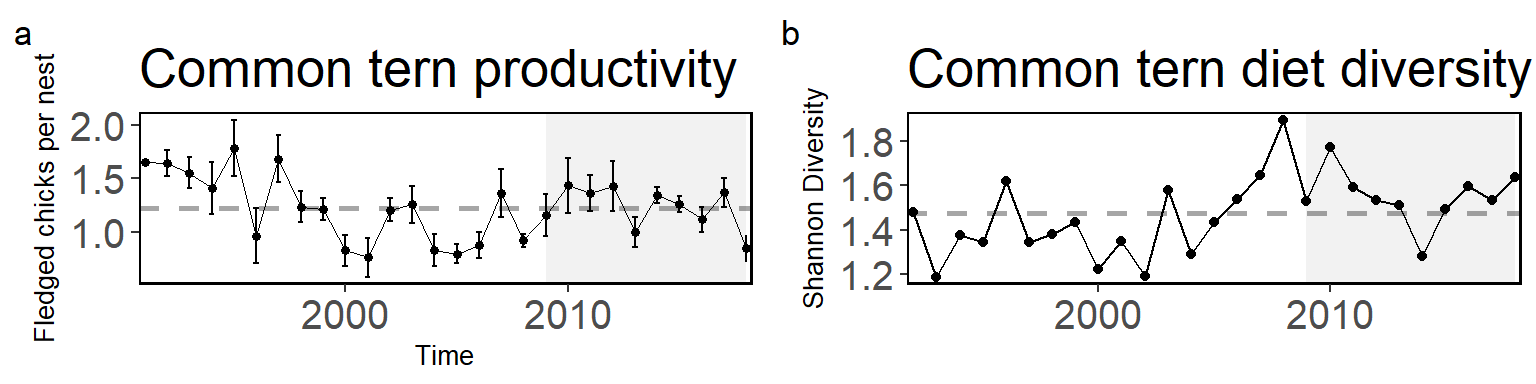
\includegraphics{C:/Users/kimberly.bastille/Desktop/tech-doc/imagesunnamed-chunk-55-1} 

}

\caption{a. Mean common tern productivity at nesting sites in Gulf of Maine. Error bars show +/- 1 SE of the mean. b. Shannon diversity of common tern diets observed at nesting sites in Gulf of Maine. Diversity of common tern diets has been predominantly above the long-term mean since 2006.}\label{fig:unnamed-chunk-55}
\end{figure}

Along with nest productivity and diet diversity indices, we presented
maps of sampling sites in Gulf of Maine and mean prey frequencies across
sites. Prey occurring in less than 5\% of common tern diets was excluded
for visual clarity.

\begin{Shaded}
\begin{Highlighting}[]
\CommentTok{#Map subfig}
\CommentTok{# Set lat/lon window for maps}
\NormalTok{xmin =}\StringTok{ }\OperatorTok{-}\FloatTok{70.5}
\NormalTok{xmax =}\StringTok{ }\OperatorTok{-}\FloatTok{68.25}
\NormalTok{ymin =}\StringTok{ }\DecValTok{43}
\NormalTok{ymax =}\StringTok{ }\FloatTok{44.5}
\NormalTok{xlims <-}\StringTok{ }\KeywordTok{c}\NormalTok{(xmin, xmax)}
\NormalTok{ylims <-}\StringTok{ }\KeywordTok{c}\NormalTok{(ymin, ymax)}
\NormalTok{island_loc <-}\StringTok{ }\KeywordTok{data.frame}\NormalTok{(}\DataTypeTok{Island =} \KeywordTok{c}\NormalTok{(}\StringTok{"EER"}\NormalTok{,}\StringTok{"JI"}\NormalTok{,}\StringTok{"MR"}\NormalTok{,}\StringTok{"OGI"}\NormalTok{,}
                                    \StringTok{"PINWR"}\NormalTok{,}\StringTok{"SINWR"}\NormalTok{,}\StringTok{"STI"}\NormalTok{),}
                         \DataTypeTok{Latitude =} \KeywordTok{c}\NormalTok{(}\FloatTok{43.861}\NormalTok{,}\FloatTok{43.764}\NormalTok{,}\FloatTok{43.785}\NormalTok{,}\FloatTok{43.650}\NormalTok{,}
                                      \FloatTok{43.739}\NormalTok{,}\FloatTok{43.886}\NormalTok{,}\FloatTok{43.505}\NormalTok{),}
                         \DataTypeTok{Longitude =} \KeywordTok{c}\NormalTok{(}\OperatorTok{-}\FloatTok{69.382}\NormalTok{,}\OperatorTok{-}\FloatTok{69.909}\NormalTok{,}\OperatorTok{-}\FloatTok{68.854}\NormalTok{,}\OperatorTok{-}\FloatTok{70.124}\NormalTok{,}
                                       \OperatorTok{-}\FloatTok{69.771}\NormalTok{,}\OperatorTok{-}\FloatTok{68.742}\NormalTok{,}\OperatorTok{-}\FloatTok{70.312}\NormalTok{))}
\NormalTok{islands <-}\StringTok{ }\KeywordTok{ggplot}\NormalTok{() }\OperatorTok{+}
\StringTok{  }\KeywordTok{geom_sf}\NormalTok{(}\DataTypeTok{data =}\NormalTok{ new_england, }\DataTypeTok{size =}\NormalTok{ map.lwd) }\OperatorTok{+}
\StringTok{  }\KeywordTok{geom_point}\NormalTok{(}\DataTypeTok{data =}\NormalTok{ island_loc, }\KeywordTok{aes}\NormalTok{(}\DataTypeTok{x =}\NormalTok{ Longitude, }\DataTypeTok{y =}\NormalTok{ Latitude)) }\OperatorTok{+}
\StringTok{  }\KeywordTok{geom_label_repel}\NormalTok{(}\DataTypeTok{data =}\NormalTok{ island_loc, }\KeywordTok{aes}\NormalTok{(}\DataTypeTok{x =}\NormalTok{ Longitude, }\DataTypeTok{y =}\NormalTok{ Latitude,}
                                          \DataTypeTok{label =}\NormalTok{ Island), }\DataTypeTok{nudge_y  =} \OperatorTok{-}\FloatTok{0.1}\NormalTok{, }
                   \DataTypeTok{size =} \FloatTok{2.5}\NormalTok{) }\OperatorTok{+}
\StringTok{  }\KeywordTok{coord_sf}\NormalTok{(}\DataTypeTok{crs =}\NormalTok{ crs, }\DataTypeTok{xlim =}\NormalTok{ xlims, }\DataTypeTok{ylim =}\NormalTok{ ylims) }\OperatorTok{+}
\StringTok{  }\KeywordTok{theme_map}\NormalTok{() }\OperatorTok{+}
\StringTok{  }\KeywordTok{ggtitle}\NormalTok{(}\StringTok{"Common tern study sites"}\NormalTok{) }\OperatorTok{+}
\StringTok{  }\KeywordTok{xlab}\NormalTok{(}\StringTok{"Longitude"}\NormalTok{) }\OperatorTok{+}
\StringTok{  }\KeywordTok{ylab}\NormalTok{(}\StringTok{"Latitude"}\NormalTok{) }\OperatorTok{+}
\StringTok{  }\KeywordTok{labs}\NormalTok{(}\DataTypeTok{tag =} \StringTok{"a"}\NormalTok{)  }\OperatorTok{+}
\StringTok{  }\KeywordTok{theme}\NormalTok{(}\DataTypeTok{panel.border =} \KeywordTok{element_rect}\NormalTok{(}\DataTypeTok{colour =} \StringTok{"black"}\NormalTok{, }\DataTypeTok{fill=}\OtherTok{NA}\NormalTok{, }\DataTypeTok{size=}\FloatTok{0.75}\NormalTok{),}
        \DataTypeTok{legend.key =} \KeywordTok{element_blank}\NormalTok{(),}
        \DataTypeTok{axis.title =} \KeywordTok{element_text}\NormalTok{(}\DataTypeTok{size =} \DecValTok{11}\NormalTok{),}
        \DataTypeTok{strip.background =} \KeywordTok{element_blank}\NormalTok{(),}
        \DataTypeTok{strip.text=}\KeywordTok{element_text}\NormalTok{(}\DataTypeTok{hjust=}\DecValTok{0}\NormalTok{),}
        \DataTypeTok{axis.text =} \KeywordTok{element_text}\NormalTok{(}\DataTypeTok{size =} \DecValTok{8}\NormalTok{))}
\CommentTok{# inset_states <- new_england %>% filter(STATE_NAME %in% c("Maine",}
\CommentTok{#                                                          "New Hampshire",}
\CommentTok{#                                                          "Massachusetts"))}
\CommentTok{# Set lat/lon window for maps}
\NormalTok{xmin2 =}\StringTok{ }\OperatorTok{-}\DecValTok{72}
\NormalTok{xmax2 =}\StringTok{ }\OperatorTok{-}\FloatTok{66.25}
\NormalTok{ymin2 =}\StringTok{ }\FloatTok{42.5}
\NormalTok{ymax2 =}\StringTok{ }\FloatTok{47.5}
\NormalTok{xlims2 <-}\StringTok{ }\KeywordTok{c}\NormalTok{(xmin2, xmax2)}
\NormalTok{ylims2 <-}\StringTok{ }\KeywordTok{c}\NormalTok{(ymin2, ymax2)}
\NormalTok{NE <-}\StringTok{ }\KeywordTok{ggplotGrob}\NormalTok{(}
\KeywordTok{ggplot}\NormalTok{()}\OperatorTok{+}
\StringTok{  }\KeywordTok{geom_sf}\NormalTok{(}\DataTypeTok{data =}\NormalTok{ new_england, }\DataTypeTok{size =}\NormalTok{ map.lwd) }\OperatorTok{+}
\StringTok{  }\KeywordTok{coord_sf}\NormalTok{(}\DataTypeTok{crs =}\NormalTok{ crs, }\DataTypeTok{xlim =}\NormalTok{ xlims2, }\DataTypeTok{ylim =}\NormalTok{ ylims2) }\OperatorTok{+}
\StringTok{  }\KeywordTok{annotate}\NormalTok{(}\StringTok{"rect"}\NormalTok{, }\DataTypeTok{xmin =}\NormalTok{ xmin, }\DataTypeTok{xmax =}\NormalTok{ xmax, }\DataTypeTok{ymin =}\NormalTok{ ymin, }\DataTypeTok{ymax =}\NormalTok{ ymax, }\DataTypeTok{color =} \StringTok{"black"}\NormalTok{,}
           \DataTypeTok{size =} \FloatTok{0.1}\NormalTok{, }\DataTypeTok{fill =} \StringTok{"transparent"}\NormalTok{) }\OperatorTok{+}
\StringTok{  }\KeywordTok{theme_map}\NormalTok{() }\OperatorTok{+}
\StringTok{  }\KeywordTok{xlab}\NormalTok{(}\StringTok{""}\NormalTok{) }\OperatorTok{+}
\StringTok{  }\KeywordTok{ylab}\NormalTok{(}\StringTok{""}\NormalTok{) }\OperatorTok{+}
\StringTok{  }\KeywordTok{theme}\NormalTok{(}\DataTypeTok{panel.border =} \KeywordTok{element_rect}\NormalTok{(}\DataTypeTok{colour =} \StringTok{"black"}\NormalTok{, }\DataTypeTok{fill =} \StringTok{"transparent"}\NormalTok{, }\DataTypeTok{size=}\FloatTok{0.75}\NormalTok{),}
        \DataTypeTok{plot.background =} \KeywordTok{element_rect}\NormalTok{(}\DataTypeTok{fill =} \StringTok{"transparent"}\NormalTok{, }\DataTypeTok{colour =} \OtherTok{NA}\NormalTok{),}
        \DataTypeTok{legend.key =} \KeywordTok{element_blank}\NormalTok{(),}
        \DataTypeTok{axis.title =} \KeywordTok{element_text}\NormalTok{(}\DataTypeTok{size =} \DecValTok{11}\NormalTok{),}
        \DataTypeTok{strip.background =} \KeywordTok{element_blank}\NormalTok{(),}
        \DataTypeTok{strip.text=}\KeywordTok{element_text}\NormalTok{(}\DataTypeTok{hjust=}\DecValTok{0}\NormalTok{),}
        \DataTypeTok{axis.text =} \KeywordTok{element_blank}\NormalTok{())}
\NormalTok{)}
\NormalTok{full_map <-}\StringTok{ }\NormalTok{islands }\OperatorTok{+}
\StringTok{  }\KeywordTok{annotation_custom}\NormalTok{(}\DataTypeTok{grob =}\NormalTok{ NE, }\DataTypeTok{xmin =} \OperatorTok{-}\DecValTok{69}\NormalTok{, }\DataTypeTok{xmax =} \OperatorTok{-}\FloatTok{68.25}\NormalTok{, }\DataTypeTok{ymin =} \FloatTok{42.9}\NormalTok{, }\DataTypeTok{ymax =} \FloatTok{43.6}\NormalTok{)}


\CommentTok{# Prey freq stacked bar}
\NormalTok{prey_freq <-}\StringTok{ }\NormalTok{ecodata}\OperatorTok{::}\NormalTok{common_tern }\OperatorTok\StringTok{ }
\StringTok{  }\KeywordTok{filter}\NormalTok{(}\KeywordTok{str_detect}\NormalTok{(Var, }\StringTok{"Diet"}\NormalTok{),}
         \OperatorTok{!}\KeywordTok{str_detect}\NormalTok{(Var, }\StringTok{"Sum"}\NormalTok{)) }\OperatorTok\StringTok{ }
\StringTok{    }\KeywordTok{mutate}\NormalTok{(}\DataTypeTok{Island =} \KeywordTok{word}\NormalTok{(Var, }\DecValTok{1}\NormalTok{),}
         \DataTypeTok{Var =} \KeywordTok{word}\NormalTok{(Var, }\DecValTok{4}\NormalTok{)) }\OperatorTok
\StringTok{    }\KeywordTok{group_by}\NormalTok{(Var, Time) }\OperatorTok\StringTok{ }
\StringTok{    }\NormalTok{dplyr}\OperatorTok{::}\KeywordTok{summarise}\NormalTok{(}\DataTypeTok{Value =} \KeywordTok{sum}\NormalTok{(Value, }\DataTypeTok{na.rm =}\NormalTok{ T)) }\OperatorTok\StringTok{ }
\StringTok{    }\KeywordTok{group_by}\NormalTok{(Time) }\OperatorTok\StringTok{ }
\StringTok{    }\KeywordTok{mutate}\NormalTok{(}\DataTypeTok{Freq =}\NormalTok{ Value}\OperatorTok{/}\KeywordTok{sum}\NormalTok{(Value, }\DataTypeTok{na.rm =}\NormalTok{ T)) }\OperatorTok\StringTok{ }
\StringTok{    }\KeywordTok{group_by}\NormalTok{(Var) }\OperatorTok\StringTok{ }
\StringTok{  }\KeywordTok{mutate}\NormalTok{(}\DataTypeTok{hline =} \KeywordTok{mean}\NormalTok{(Freq, }\DataTypeTok{na.rm =}\NormalTok{ T))}

\NormalTok{diet_freq_bar <-}\StringTok{ }\NormalTok{prey_freq }\OperatorTok\StringTok{ }
\StringTok{  }\KeywordTok{filter}\NormalTok{(Freq }\OperatorTok{>}\StringTok{ }\FloatTok{0.05}\NormalTok{) }\OperatorTok\StringTok{ }
\StringTok{  }\NormalTok{dplyr}\OperatorTok{::}\KeywordTok{mutate}\NormalTok{(}\DataTypeTok{Prey =} \KeywordTok{gsub}\NormalTok{(}\StringTok{"}\CharTok{\textbackslash{}\textbackslash{}}\StringTok{."}\NormalTok{, }\StringTok{" "}\NormalTok{, Var)) }\OperatorTok\StringTok{ }
\StringTok{  }\NormalTok{dplyr}\OperatorTok{::}\KeywordTok{mutate}\NormalTok{(}\DataTypeTok{Prey =} \KeywordTok{gsub}\NormalTok{(}\StringTok{"Invertebrate"}\NormalTok{, }\StringTok{"Invert."}\NormalTok{, Prey)) }\OperatorTok\StringTok{ }
\StringTok{  }\CommentTok{# dplyr::rename(Prey = Var) %>%}
\StringTok{  }\KeywordTok{ggplot}\NormalTok{(}\KeywordTok{aes}\NormalTok{(}\DataTypeTok{x =}\NormalTok{ Time, }\DataTypeTok{y =}\NormalTok{ Freq, }\DataTypeTok{fill =}\NormalTok{ Prey)) }\OperatorTok{+}
\StringTok{  }\KeywordTok{geom_bar}\NormalTok{(}\DataTypeTok{stat =} \StringTok{"identity"}\NormalTok{) }\OperatorTok{+}
\StringTok{    }\CommentTok{# geom_bar_interactive(aes(tooltip = paste(Prey,round(Freq,2),Time)),stat = "identity") +}
\StringTok{  }\KeywordTok{scale_fill_manual}\NormalTok{(}\DataTypeTok{values =}\NormalTok{ RColorBrewer}\OperatorTok{::}\KeywordTok{brewer.pal}\NormalTok{(}\DecValTok{10}\NormalTok{,}\StringTok{"Paired"}\NormalTok{)) }\OperatorTok{+}
\StringTok{  }\KeywordTok{ggtitle}\NormalTok{(}\StringTok{"Prey composition"}\NormalTok{) }\OperatorTok{+}
\StringTok{  }\KeywordTok{ylab}\NormalTok{(}\StringTok{"Proportion of prey items"}\NormalTok{) }\OperatorTok{+}
\StringTok{  }\KeywordTok{labs}\NormalTok{(}\DataTypeTok{tag =} \StringTok{"b"}\NormalTok{)  }\OperatorTok{+}
\StringTok{  }\KeywordTok{theme_ts}\NormalTok{() }\OperatorTok{+}\StringTok{ }
\StringTok{  }\KeywordTok{theme}\NormalTok{(}\DataTypeTok{legend.text =} \KeywordTok{element_text}\NormalTok{(}\DataTypeTok{size =} \DecValTok{8}\NormalTok{))}


\CommentTok{# diet_freq_bar <- girafe(ggobj = diet_freq_bar)}
\CommentTok{# diet_freq_bar <- girafe_options(diet_freq_bar, opts_zoom(max = 5) )}

\NormalTok{full_map }\OperatorTok{+}\StringTok{ }\NormalTok{diet_freq_bar }\OperatorTok{+}\StringTok{ }\KeywordTok{plot_layout}\NormalTok{(}\DataTypeTok{ncol =} \DecValTok{2}\NormalTok{, }\DataTypeTok{widths=}\KeywordTok{c}\NormalTok{(}\DecValTok{4}\NormalTok{,}\DecValTok{4}\NormalTok{))}
\end{Highlighting}
\end{Shaded}

\begin{figure}

{\centering 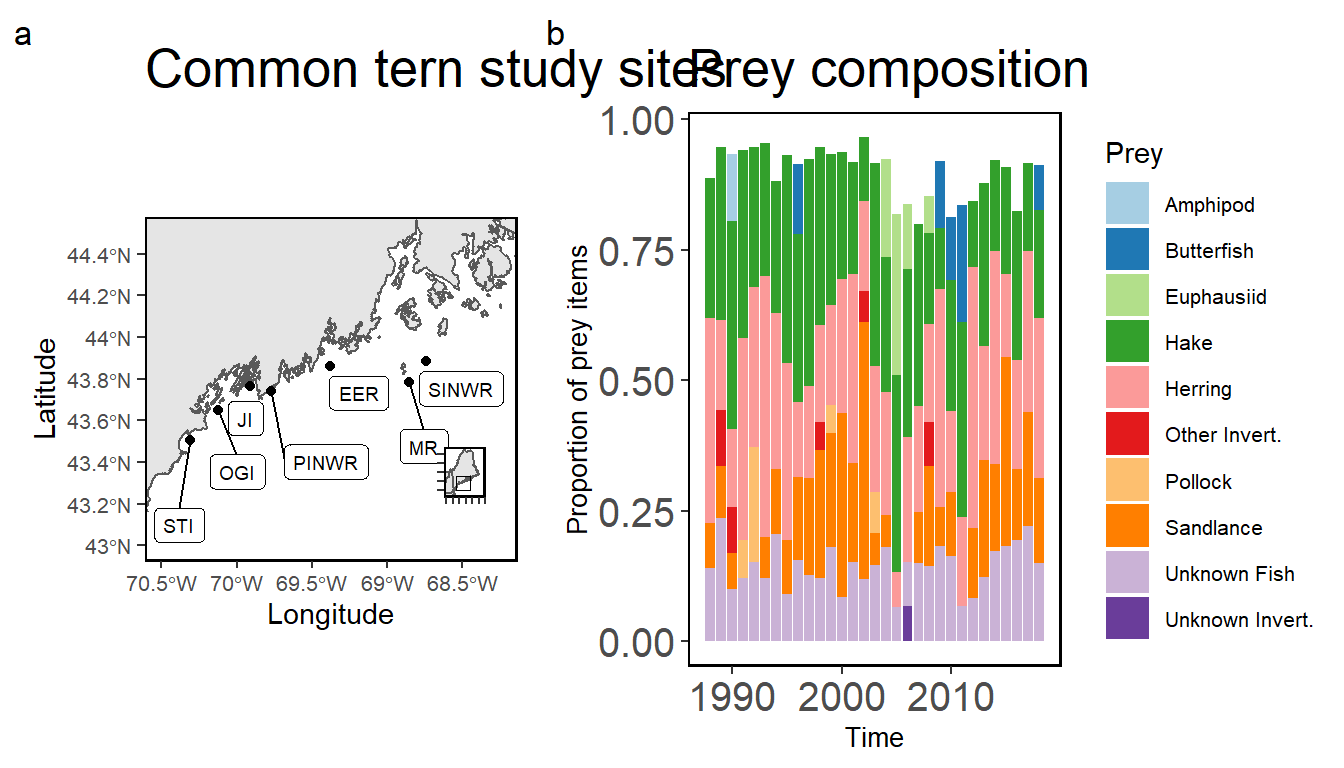
\includegraphics{C:/Users/kimberly.bastille/Desktop/tech-doc/imagesunnamed-chunk-56-1} 

}

\caption{Common terns: a. Locations of the seven sampled common tern nesting sites in Gulf of Maine (EER = Eastern Egg Rock, JI = Jenny Island, MR = Matinicus Rock, OGI = Outer Green Island, PINWR = Pond Island National Wildlife Refuge, SINWR = Seal Island National Wildlife Refuge, STI = Stratton Island), and b. Prey frequencies in the diets of common tern observed across the seven colonies in Gulf of Maine. Prey occurring in <5\% of common tern diets were excluded for clarity.}\label{fig:unnamed-chunk-56}
\end{figure}

\chapter{Seasonal SST Anomalies}\label{seasonal-sst-anomalies}

\textbf{Description}: Seasonal SST Anomalies

\textbf{Indicator category}: Database pull with analysis

\textbf{Found in}: State of the Ecosystem - Gulf of Maine \& Georges
Bank (2018, 2019), State of the Ecosystem - Mid-Atlantic (2018, 2019)

\textbf{Contributor(s)}: Sean Hardison, Vincent Saba

\textbf{Data steward}: Sean Hardison,
\href{mailto:sean.hardison@noaa.gov}{\nolinkurl{sean.hardison@noaa.gov}}

\textbf{Point of contact}: Sean Hardison,
\href{mailto:sean.hardison@noaa.gov}{\nolinkurl{sean.hardison@noaa.gov}}

\textbf{Public availability statement}: Source data are available
\href{https://www.esrl.noaa.gov/psd/data/gridded/data.noaa.oisst.v2.highres.html}{here}.

\section{Methods}\label{methods-25}

\subsection{Data sources}\label{data-sources-25}

Data for seasonal sea surface tempature anomalies (Fig.
\ref{fig:MAB-SST-insitu}) were derived from the NOAA optimum
interpolation sea surface temperature high resolution data set
(\href{https://www.esrl.noaa.gov/psd/data/gridded/data.noaa.oisst.v2.highres.html}{NOAA
OISST V2}) provided by NOAA/OAR/ESRL PSD, Boulder, CO. The data extend
from 1981 to present, and provide a 0.25° x 0.25° global grid of SST
measurements (Reynolds et al.
\protect\hyperlink{ref-Reynolds2007}{2007}).

\subsection{Data extraction}\label{data-extraction-20}

Individual files containing daily mean SST data for each year during the
period of 1981-present were downloaded from the
\href{https://www.esrl.noaa.gov/psd/data/gridded/data.noaa.oisst.v2.highres.html}{OI
SST V5 site}. Yearly data provided as layered rasters were masked
according to the extent of Northeast US Continental Shelf. Data were
split into three month seasons for (Winter = Jan, Feb, Mar; Spring =
Apr, May, Jun; Summer = July, August, September; Fall = Oct, Nov, Dec).

\subsection{Data analysis}\label{data-analysis-23}

We calculated the long-term mean (LTM) for each season-specific stack of
rasters over the period of 1982-2010, and then subtracted the (LTM) from
daily mean SST values to find the SST anomaly for a given year. The use
of climatological reference periods is a standard procedure for the
calculation of meteorological anomalies (WMO
\protect\hyperlink{ref-WMO2017}{2017}). Prior to 2019 State of the
Ecosystem reports, SST anomaly information made use of a 1982-2012
reference period. A 1982-2010 reference period was adopted to facilitate
calculating anomalies from a standard
\href{https://www.esrl.noaa.gov/psd/data/gridded/data.noaa.oisst.v2.highres.html}{NOAA
ESRL} data set.

R code used in extraction and processing:

\begin{Shaded}
\begin{Highlighting}[]
\CommentTok{#Processing for spatial SST anomaly}

\KeywordTok{library}\NormalTok{(dplyr)}
\KeywordTok{library}\NormalTok{(raster)}
\KeywordTok{library}\NormalTok{(sf)}
\KeywordTok{library}\NormalTok{(ggplot2)}
\KeywordTok{library}\NormalTok{(ncdf4)}
\KeywordTok{library}\NormalTok{(reshape2)}

\NormalTok{rast_prep <-}\StringTok{ }\ControlFlowTok{function}\NormalTok{(r)\{}
\NormalTok{  r <-}\StringTok{ }\KeywordTok{rotate}\NormalTok{(r) }\CommentTok{#Rotate}
\NormalTok{  r <-}\StringTok{ }\KeywordTok{crop}\NormalTok{(r, }\KeywordTok{extent}\NormalTok{(}\OperatorTok{-}\DecValTok{77}\NormalTok{,}\OperatorTok{-}\DecValTok{60}\NormalTok{,}\DecValTok{35}\NormalTok{,}\DecValTok{46}\NormalTok{)) }\CommentTok{#Crop}
  \KeywordTok{return}\NormalTok{(r)}
\NormalTok{\}}

\NormalTok{raw.dir <-}\StringTok{ "~/git/ecodata/inst/extdata/gridded"}
\NormalTok{crs <-}\StringTok{ "+proj=longlat +lat_1=35 +lat_2=45 +lat_0=40}
\StringTok{+lon_0=-77 +x_0=0 +y_0=0 +datum=NAD83 +no_defs +ellps=GRS80 +towgs84=0,0,0"}


\CommentTok{#These data are large files that are not included among ecodata source files. They are accessible}
\CommentTok{#here: https://www.esrl.noaa.gov/psd/data/gridded/data.noaa.oisst.v2.highres.html}
\NormalTok{sst.}\DecValTok{2018}\NormalTok{ <-}\StringTok{ }\KeywordTok{rast_prep}\NormalTok{(}\KeywordTok{stack}\NormalTok{(}\KeywordTok{file.path}\NormalTok{(raw.dir, }\StringTok{"sst.day.mean.2018.nc"}\NormalTok{)))}
\NormalTok{ltm <-}\StringTok{ }\KeywordTok{rast_prep}\NormalTok{(}\KeywordTok{stack}\NormalTok{(}\KeywordTok{file.path}\NormalTok{(raw.dir, }\StringTok{"sst.day.mean.ltm.1982-2010.nc"}\NormalTok{)))}

\CommentTok{# save(sst.2018, file = "~/git/ecodata/inst/extdata/gridded/SST.2018.rdata")}
\CommentTok{# save(sst.2018, file = "~/git/ecodata/inst/extdata/gridded/SST.LTM.rdata")}

\NormalTok{winter.ltm <-}\StringTok{ }\NormalTok{ltm[[}\DecValTok{1}\OperatorTok{:}\DecValTok{90}\NormalTok{]] }
\NormalTok{spring.ltm <-}\StringTok{ }\NormalTok{ltm[[}\DecValTok{91}\OperatorTok{:}\DecValTok{181}\NormalTok{]]}
\NormalTok{summer.ltm <-}\StringTok{ }\NormalTok{ltm[[}\DecValTok{182}\OperatorTok{:}\DecValTok{273}\NormalTok{]]}
\NormalTok{fall.ltm <-}\StringTok{ }\NormalTok{ltm[[}\DecValTok{274}\OperatorTok{:}\DecValTok{365}\NormalTok{]]}

\NormalTok{winter.anom <-}\StringTok{ }\NormalTok{sst.}\DecValTok{2018}\NormalTok{[[}\DecValTok{1}\OperatorTok{:}\DecValTok{90}\NormalTok{]] }\OperatorTok{-}\StringTok{ }\NormalTok{winter.ltm}
\NormalTok{spring.anom <-}\StringTok{ }\NormalTok{sst.}\DecValTok{2018}\NormalTok{[[}\DecValTok{91}\OperatorTok{:}\DecValTok{181}\NormalTok{]] }\OperatorTok{-}\StringTok{ }\NormalTok{spring.ltm}
\NormalTok{summer.anom <-}\StringTok{ }\NormalTok{sst.}\DecValTok{2018}\NormalTok{[[}\DecValTok{182}\OperatorTok{:}\DecValTok{273}\NormalTok{]] }\OperatorTok{-}\StringTok{ }\NormalTok{summer.ltm}
\NormalTok{fall.anom <-}\StringTok{ }\NormalTok{sst.}\DecValTok{2018}\NormalTok{[[}\DecValTok{274}\OperatorTok{:}\DecValTok{365}\NormalTok{]] }\OperatorTok{-}\StringTok{ }\NormalTok{fall.ltm}


\NormalTok{rast_process <-}\StringTok{ }\ControlFlowTok{function}\NormalTok{(r, season)\{}
\NormalTok{  r <-}\StringTok{ }\KeywordTok{stackApply}\NormalTok{(r, }\DataTypeTok{indices =} \KeywordTok{rep}\NormalTok{(}\DecValTok{1}\NormalTok{,}\KeywordTok{nlayers}\NormalTok{(r)),mean) }\CommentTok{#Find mean anomaly}
  \KeywordTok{crs}\NormalTok{(r) <-}\StringTok{ }\NormalTok{crs }\CommentTok{#Add SOE CRS}
\NormalTok{  r <-}\StringTok{ }\KeywordTok{disaggregate}\NormalTok{(r, }\DecValTok{5}\NormalTok{) }\CommentTok{#interpolate step 1 - create higher res grid}
\NormalTok{  r <-}\StringTok{ }\KeywordTok{focal}\NormalTok{(r, }\DataTypeTok{w=}\KeywordTok{matrix}\NormalTok{(}\DecValTok{1}\NormalTok{,}\DataTypeTok{nrow=}\DecValTok{5}\NormalTok{,}\DataTypeTok{ncol=}\DecValTok{5}\NormalTok{), }\DataTypeTok{fun=}\NormalTok{mean,}
             \DataTypeTok{na.rm=}\OtherTok{TRUE}\NormalTok{, }\DataTypeTok{pad=}\OtherTok{TRUE}\NormalTok{) }\CommentTok{#interpolate step 2 - moving window}
\NormalTok{  r <-}\StringTok{ }\KeywordTok{as}\NormalTok{(r, }\StringTok{"SpatialPointsDataFrame"}\NormalTok{) }\CommentTok{#Convert to ggplot-able object}
\NormalTok{  r <-}\StringTok{ }\KeywordTok{as.data.frame}\NormalTok{(r)}
\NormalTok{  r <-}\StringTok{ }\NormalTok{r }\OperatorTok
\StringTok{    }\NormalTok{reshape2}\OperatorTok{::}\KeywordTok{melt}\NormalTok{(}\DataTypeTok{id =} \KeywordTok{c}\NormalTok{(}\StringTok{"y"}\NormalTok{,}\StringTok{"x"}\NormalTok{)) }\OperatorTok
\StringTok{    }\NormalTok{dplyr}\OperatorTok{::}\KeywordTok{rename}\NormalTok{(}\DataTypeTok{Latitude =}\NormalTok{ y, }\DataTypeTok{Longitude =}\NormalTok{ x) }\OperatorTok
\StringTok{    }\NormalTok{dplyr}\OperatorTok{::}\KeywordTok{select}\NormalTok{(}\OperatorTok{-}\NormalTok{variable) }\OperatorTok\StringTok{ }
\StringTok{    }\KeywordTok{mutate}\NormalTok{(}\DataTypeTok{Season =}\NormalTok{ season) }\OperatorTok\StringTok{ }
\StringTok{    }\NormalTok{dplyr}\OperatorTok{::}\KeywordTok{rename}\NormalTok{(}\DataTypeTok{Value =}\NormalTok{ value)}
    
  \KeywordTok{return}\NormalTok{(r)}
\NormalTok{\}}

\NormalTok{seasonal_sst_anomaly_gridded <-}\StringTok{ }
\StringTok{  }\KeywordTok{rbind}\NormalTok{(}\KeywordTok{rast_process}\NormalTok{(winter.anom,}\DataTypeTok{season =} \StringTok{"Winter"}\NormalTok{),}
      \KeywordTok{rast_process}\NormalTok{(spring.anom,}\DataTypeTok{season =} \StringTok{"Spring"}\NormalTok{),}
      \KeywordTok{rast_process}\NormalTok{(summer.anom, }\DataTypeTok{season =} \StringTok{"Summer"}\NormalTok{),}
      \KeywordTok{rast_process}\NormalTok{(fall.anom, }\DataTypeTok{season =} \StringTok{"Fall"}\NormalTok{))}

\NormalTok{usethis}\OperatorTok{::}\KeywordTok{use_data}\NormalTok{(seasonal_sst_anomaly_gridded, }\DataTypeTok{overwrite =}\NormalTok{ T)}
\end{Highlighting}
\end{Shaded}

\subsection{Plotting}\label{plotting-17}

\begin{figure}
\centering
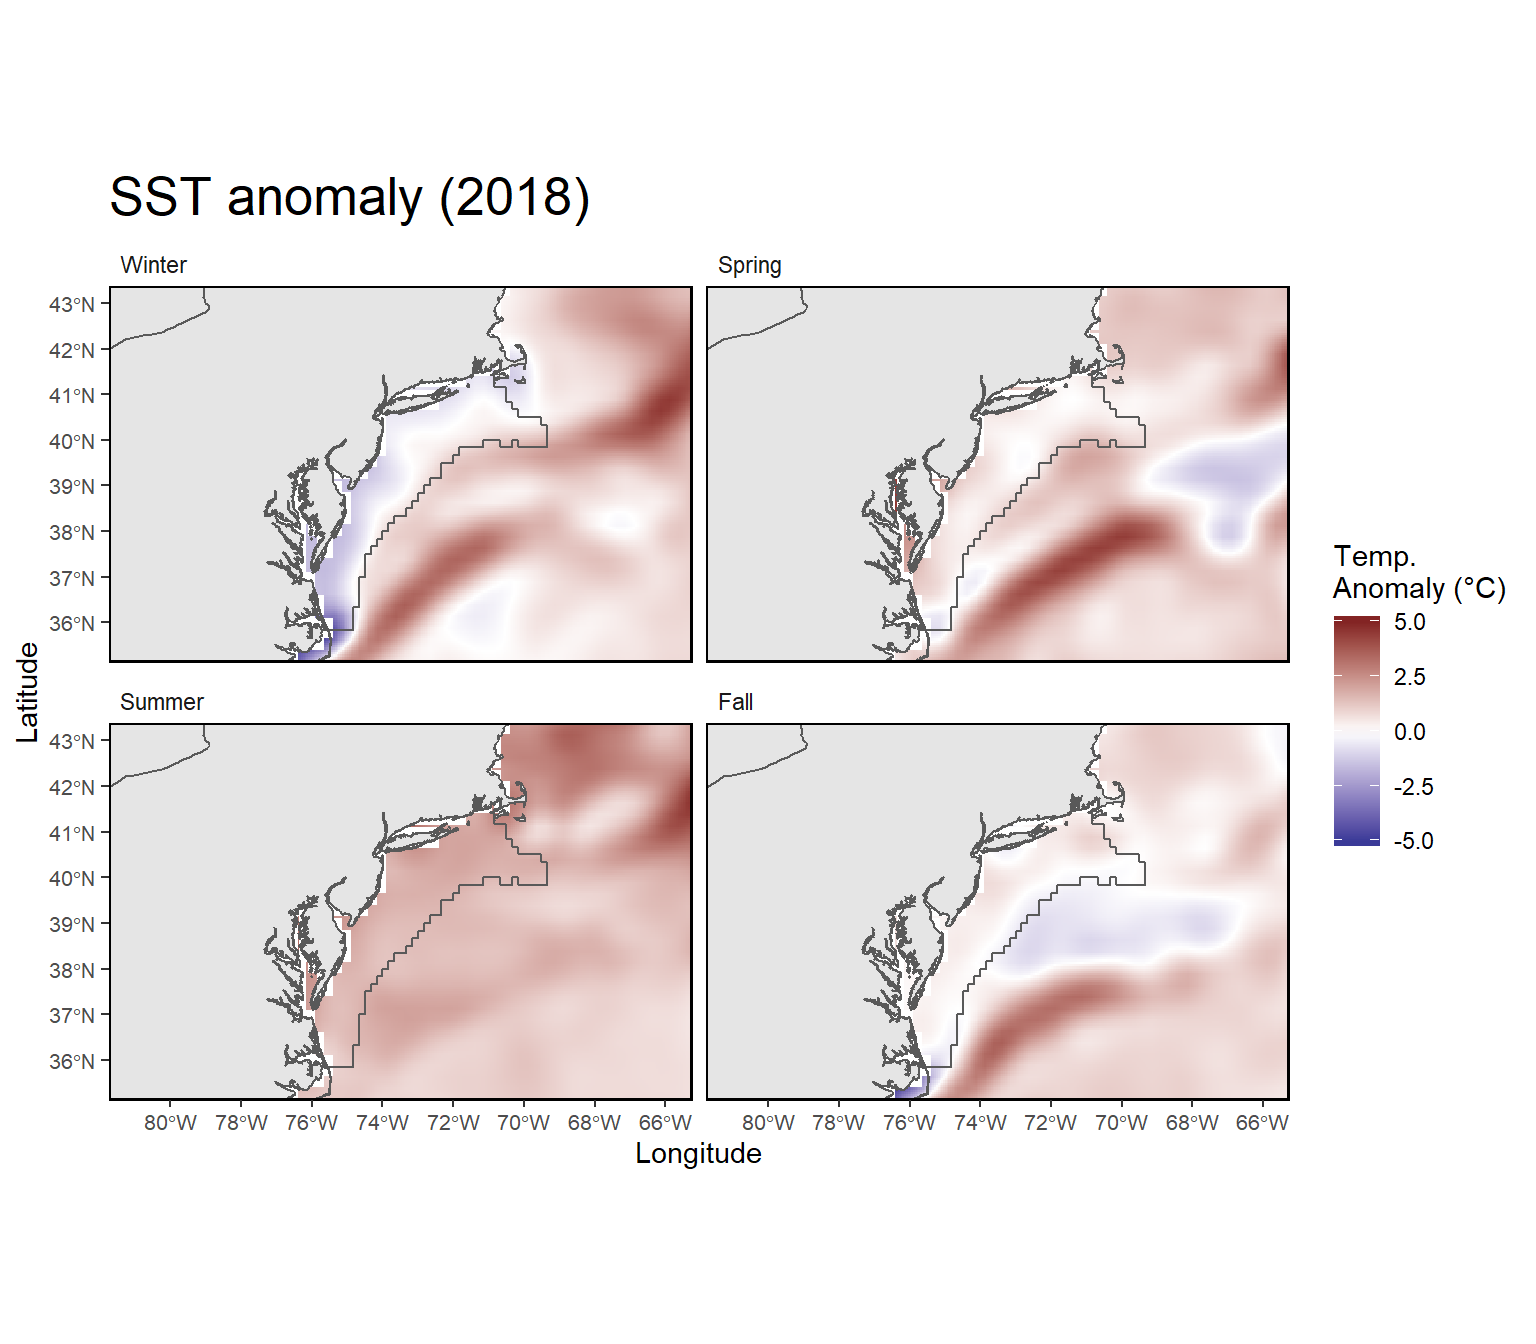
\includegraphics{C:/Users/kimberly.bastille/Desktop/tech-doc/imagesMAB-SST-1.pdf}
\caption{\label{fig:MAB-SST}Seasonal sea-surface temperature anomalies in
the Mid-Atlantic Bight.}
\end{figure}

\chapter{Single Species Status Indicator}\label{stockstatus}

\textbf{Description}: Summary of the most recent stock assessment
results for each assessed species.

\textbf{Found in}: State of the Ecosystem - Gulf of Maine \& Georges
Bank (2017, 2018, 2019), State of the Ecosystem - Mid-Atlantic (2017,
2018, 2019)

\textbf{Indicator category}: Synthesis of published information

\textbf{Contributor(s)}: Sarah Gaichas, based on code and spreadsheets
originally provided by Chris Legault

\textbf{Data steward}: Sarah Gaichas
\href{mailto:sarah.gaichas@noaa.gov}{\nolinkurl{sarah.gaichas@noaa.gov}}

\textbf{Point of contact}: Sarah Gaichas
\href{mailto:sarah.gaichas@noaa.gov}{\nolinkurl{sarah.gaichas@noaa.gov}}

\textbf{Public availability statement}: All stock assessment results are
publicly available (see Data Sources). Summarized data are available
\href{http://comet.nefsc.noaa.gov/erddap/tabledap/assess_soe_v1.htmlTable?No,Entity_Name,Science_Center,Assessment_Year,Last_Data_Year,Assessment_Level,Citation,Comments,Best_F,F_Year,Flimit,Fmsy,F_Flimit,F_Fmsy,Best_B,B_Year,B_Blimit,B_Bmsy,Stock_Level_Relative_to_Bmsy,Bmsy,Blim}{here}.

\section{Methods}\label{methods-26}

\subsection{Data sources}\label{data-sources-26}

``Data'' used for this indicator are the outputs of stock assessment
models and review processes, including reference points (proxies for
fishing mortality limits and stock biomass targets and limits), and the
current fishing mortality rate and biomass of each stock. The
spreadsheet summarizes the most recent stock assessment updates for each
species, which are available on the Northeast Fisheries Science Center
(NEFSC) website at: \url{https://www.nefsc.noaa.gov/saw/reports.html}\\
\url{https://www.nefsc.noaa.gov/publications/crd/crd1717/}

Additional assessments are reported directly to the New England Fishery
Management Council (NEFMC):
\url{http://s3.amazonaws.com/nefmc.org/Document-2-SAFE-Report-for-Fishing-Year-2016.pdf}\\
\url{http://s3.amazonaws.com/nefmc.org/4_NEFSC_SkateMemo_July_2017.pdf}

\subsection{Data extraction}\label{data-extraction-21}

Each assessment document was searched to find the following information
(often but not always summarized under a term of reference to determine
stock status in the executive summary):

\begin{itemize}
\item
  \textbf{Bcur}: current year biomass, (most often spawning stock
  biomass (SSB) or whatever units the reference points are in)
\item
  \textbf{Fcur}: current year fishing mortality, F
\item
  \textbf{Bref}: biomass reference point, a proxy of Bmsy (the target)
\item
  \textbf{Fref}: fishing mortality reference point, a proxy of Fmsy
\end{itemize}

\subsection{Data processing}\label{data-processing-16}

The following R code was used to process the stock status data set for
inclusion in the ecodata R package.

\begin{Shaded}
\begin{Highlighting}[]
\CommentTok{# Processing single-species stock mortality and biomass data}

\CommentTok{# Read more about this data at https://noaa-edab.github.io/tech-doc/stockstatus.html}

\KeywordTok{library}\NormalTok{(dplyr)}
\KeywordTok{library}\NormalTok{(tidyr)}
\KeywordTok{library}\NormalTok{(ggplot2)}

\NormalTok{data.dir <-}\StringTok{ }\NormalTok{here}\OperatorTok{::}\KeywordTok{here}\NormalTok{(}\StringTok{'inst'}\NormalTok{,}\StringTok{'extdata'}\NormalTok{)}

\NormalTok{get_stocks <-}\StringTok{ }\ControlFlowTok{function}\NormalTok{(}\DataTypeTok{save_clean =}\NormalTok{ F)\{}
\NormalTok{  assess <-}\StringTok{ }\KeywordTok{read.csv}\NormalTok{(}\KeywordTok{file.path}\NormalTok{(data.dir, }\StringTok{"2018assess.csv"}\NormalTok{))}
\NormalTok{  decode <-}\StringTok{ }\KeywordTok{read.csv}\NormalTok{(}\KeywordTok{file.path}\NormalTok{(data.dir, }\StringTok{"2018decoder.csv"}\NormalTok{))}
  
\NormalTok{  stock_status <-}\StringTok{ }
\StringTok{    }\NormalTok{assess }\OperatorTok
\StringTok{    }\KeywordTok{group_by}\NormalTok{(Entity.Name) }\OperatorTok
\StringTok{    }\KeywordTok{filter}\NormalTok{(Assessment.Year }\OperatorTok{==}\StringTok{ }\KeywordTok{max}\NormalTok{(Assessment.Year)) }\OperatorTok\StringTok{ }\CommentTok{#Find last year assessment occurred for each stock}
\StringTok{    }\KeywordTok{ungroup}\NormalTok{() }\OperatorTok\StringTok{ }
\StringTok{    }\KeywordTok{left_join}\NormalTok{(.,decode, }\DataTypeTok{by =} \StringTok{"Entity.Name"}\NormalTok{) }\OperatorTok\StringTok{ }\CommentTok{#Join in list of managed species}
\StringTok{    }\NormalTok{dplyr}\OperatorTok{::}\KeywordTok{select}\NormalTok{(Entity.Name, Assessment.Year, F.Fmsy, B.Bmsy, Council, Code) }\OperatorTok\StringTok{ }\CommentTok{#select column variables to keep}
\StringTok{    }\KeywordTok{mutate}\NormalTok{(}\DataTypeTok{id =} \DecValTok{1}\OperatorTok{:}\KeywordTok{length}\NormalTok{(Entity.Name)) }\OperatorTok\StringTok{ }
\StringTok{    }\KeywordTok{gather}\NormalTok{(.,Var, Value,}\OperatorTok{-}\NormalTok{id,}\OperatorTok{-}\NormalTok{Entity.Name,}\OperatorTok{-}\NormalTok{Assessment.Year,}\OperatorTok{-}\NormalTok{Council,}\OperatorTok{-}\NormalTok{Code) }\OperatorTok\StringTok{ }\CommentTok{#wide to long}
\StringTok{    }\NormalTok{dplyr}\OperatorTok{::}\KeywordTok{select}\NormalTok{(}\OperatorTok{-}\NormalTok{id) }\OperatorTok\StringTok{ }
\StringTok{    }\NormalTok{dplyr}\OperatorTok{::}\KeywordTok{rename}\NormalTok{(}\StringTok{`}\DataTypeTok{Last assessment}\StringTok{`}\NormalTok{ =}\StringTok{ }\NormalTok{Assessment.Year,}
                  \DataTypeTok{Stock =}\NormalTok{ Entity.Name) }\OperatorTok\StringTok{ }\CommentTok{#rename variables for clarity}
\StringTok{    }\KeywordTok{mutate}\NormalTok{(}\DataTypeTok{Units =} \StringTok{"unitless"}\NormalTok{)}
  
  \ControlFlowTok{if}\NormalTok{ (save_clean)\{}
\NormalTok{    usethis}\OperatorTok{::}\KeywordTok{use_data}\NormalTok{(stock_status, }\DataTypeTok{overwrite =}\NormalTok{ T)}
\NormalTok{  \} }\ControlFlowTok{else}\NormalTok{ \{}
    \KeywordTok{return}\NormalTok{(stock_status)}
\NormalTok{  \}}
\NormalTok{\}}
\end{Highlighting}
\end{Shaded}

\subsection{Data analysis}\label{data-analysis-24}

For each assessed species, Bcur is divided by Bref and Fcur is divided
by Fref. They are then plotted for each species on an x-y plot, with
Bcur/Bref on the x axis, and Fcur/Fref on the y axis.

\subsection{Plotting}\label{plotting-18}

The script used to develop the figure in the SOE is below, with an
example figure. Different lines are commented out of the script to
produce the Mid- Atlantic or New England figures. The positioning table
used to make the plot (the data frame named ``decoder'' below) is
available
\href{http://comet.nefsc.noaa.gov/erddap/tabledap/assess_support_soe_v1.htmlTable?Entity_Name,Count_of_No,Min_of_No2,Code,Council,my_pos,my_pos2,my_pos3}{here}.

\begin{Shaded}
\begin{Highlighting}[]
\CommentTok{#Get data, spread for plotting, and filter}
\NormalTok{stock_status <-}\StringTok{ }\NormalTok{ecodata}\OperatorTok{::}\NormalTok{stock_status }\OperatorTok
\StringTok{  }\KeywordTok{spread}\NormalTok{(.,Var,Value) }\OperatorTok\StringTok{ }
\StringTok{  }\KeywordTok{filter}\NormalTok{(Council }\OperatorTok\StringTok{ }\KeywordTok{c}\NormalTok{(}\StringTok{"NEFMC"}\NormalTok{,}\StringTok{"Both"}\NormalTok{))}

\CommentTok{#Plot constants}
\NormalTok{y.max <-}\StringTok{ }\FloatTok{4.5}
\NormalTok{x.max <-}\StringTok{ }\FloatTok{7.5}

\NormalTok{all_missing <-}\StringTok{ }\NormalTok{stock_status }\OperatorTok
\StringTok{  }\KeywordTok{filter}\NormalTok{(}\KeywordTok{is.na}\NormalTok{(B.Bmsy),}\KeywordTok{is.na}\NormalTok{(F.Fmsy)) }\OperatorTok\StringTok{ }
\StringTok{  }\NormalTok{dplyr}\OperatorTok{::}\KeywordTok{select}\NormalTok{(Code, Council)}

\NormalTok{b_missing <-}\StringTok{ }\NormalTok{stock_status }\OperatorTok
\StringTok{  }\KeywordTok{filter}\NormalTok{(}\KeywordTok{is.na}\NormalTok{(B.Bmsy), }\OperatorTok{!}\KeywordTok{is.na}\NormalTok{(F.Fmsy)) }\OperatorTok\StringTok{ }
\StringTok{  }\NormalTok{dplyr}\OperatorTok{::}\KeywordTok{select}\NormalTok{(Code, Council)}

\NormalTok{f_missing <-}\StringTok{ }\NormalTok{stock_status }\OperatorTok
\StringTok{  }\KeywordTok{filter}\NormalTok{(}\KeywordTok{is.na}\NormalTok{(F.Fmsy), }\OperatorTok{!}\KeywordTok{is.na}\NormalTok{(B.Bmsy)) }\OperatorTok\StringTok{ }
\StringTok{  }\NormalTok{dplyr}\OperatorTok{::}\KeywordTok{select}\NormalTok{(Code, Council)}

\CommentTok{#A dataframe that defines custom legend for stocks with unknown status}

\NormalTok{all.df <-}\StringTok{ }\KeywordTok{tibble}\NormalTok{(}\DataTypeTok{text =}\NormalTok{ all_missing}\OperatorTok{$}\NormalTok{Code,}
                    \DataTypeTok{x =} \KeywordTok{rep}\NormalTok{(x.max,}\KeywordTok{length}\NormalTok{(all_missing}\OperatorTok{$}\NormalTok{Code)),}
                    \DataTypeTok{y =} \KeywordTok{seq}\NormalTok{(}\FloatTok{4.35}\NormalTok{,}\FloatTok{2.85}\NormalTok{,}\OperatorTok{-}\FloatTok{0.22}\NormalTok{),}
                    \DataTypeTok{color =}\NormalTok{ all_missing}\OperatorTok{$}\NormalTok{Council)}

\NormalTok{b.df <-}\StringTok{ }\KeywordTok{tibble}\NormalTok{(}\DataTypeTok{text =}\NormalTok{ b_missing}\OperatorTok{$}\NormalTok{Code,}
                    \DataTypeTok{x =} \KeywordTok{rep}\NormalTok{(x.max}\OperatorTok{*}\FloatTok{0.8}\NormalTok{,}\KeywordTok{length}\NormalTok{(b_missing}\OperatorTok{$}\NormalTok{Code)),}
                    \DataTypeTok{y =} \KeywordTok{c}\NormalTok{(}\FloatTok{4.35}\NormalTok{,}\FloatTok{4.14}\NormalTok{),}
                    \DataTypeTok{color =}\NormalTok{ b_missing}\OperatorTok{$}\NormalTok{Council)}

\NormalTok{f.df <-}\StringTok{ }\KeywordTok{tibble}\NormalTok{(}\DataTypeTok{text =}\NormalTok{ f_missing}\OperatorTok{$}\NormalTok{Code,}
                    \DataTypeTok{x =} \KeywordTok{rep}\NormalTok{(x.max}\OperatorTok{*}\FloatTok{0.6}\NormalTok{,}\KeywordTok{length}\NormalTok{(f_missing}\OperatorTok{$}\NormalTok{Code)),}
                    \DataTypeTok{y =} \KeywordTok{seq}\NormalTok{(}\FloatTok{4.35}\NormalTok{,}\FloatTok{2.85}\NormalTok{,}\OperatorTok{-}\FloatTok{0.22}\NormalTok{),}
                    \DataTypeTok{color =}\NormalTok{ f_missing}\OperatorTok{$}\NormalTok{Council)}


\CommentTok{#Plotting code}
\KeywordTok{ggplot}\NormalTok{(}\DataTypeTok{data =}\NormalTok{ stock_status) }\OperatorTok{+}
\StringTok{  }\KeywordTok{geom_vline}\NormalTok{(}\DataTypeTok{xintercept =} \DecValTok{1}\NormalTok{, }\DataTypeTok{linetype =} \StringTok{"dotted"}\NormalTok{, }\DataTypeTok{color =} \StringTok{"grey60"}\NormalTok{)}\OperatorTok{+}
\StringTok{  }\KeywordTok{geom_vline}\NormalTok{(}\DataTypeTok{xintercept =} \FloatTok{0.5}\NormalTok{, }\DataTypeTok{linetype =} \StringTok{"dashed"}\NormalTok{, }\DataTypeTok{color =} \StringTok{"grey60"}\NormalTok{)}\OperatorTok{+}
\StringTok{  }\KeywordTok{geom_hline}\NormalTok{(}\DataTypeTok{yintercept =} \DecValTok{1}\NormalTok{, }\DataTypeTok{linetype =} \StringTok{"dashed"}\NormalTok{, }\DataTypeTok{color =} \StringTok{"grey60"}\NormalTok{) }\OperatorTok{+}
\StringTok{  }\KeywordTok{geom_point}\NormalTok{(}\KeywordTok{aes}\NormalTok{(}\DataTypeTok{x =}\NormalTok{ B.Bmsy,}
                 \DataTypeTok{y =}\NormalTok{ F.Fmsy,}
                 \DataTypeTok{color =}\NormalTok{ Council,}
                 \DataTypeTok{shape =}\NormalTok{ Council)) }\OperatorTok{+}
\StringTok{  }\KeywordTok{geom_text_repel}\NormalTok{(}\KeywordTok{aes}\NormalTok{(}\DataTypeTok{x =}\NormalTok{ B.Bmsy, }\CommentTok{#geom_text_repel auto-jitters text around points}
                      \DataTypeTok{y =}\NormalTok{ F.Fmsy,}
                      \DataTypeTok{label =}\NormalTok{ Code,}
                      \DataTypeTok{color =}\NormalTok{ Council), }\DataTypeTok{show.legend =} \OtherTok{FALSE}\NormalTok{,}\DataTypeTok{nudge_y =} \FloatTok{0.05}\NormalTok{, }\DataTypeTok{nudge_x =} \FloatTok{0.05}\NormalTok{) }\OperatorTok{+}
\StringTok{  }\KeywordTok{ylim}\NormalTok{(}\DecValTok{0}\NormalTok{,y.max) }\OperatorTok{+}
\StringTok{  }\KeywordTok{xlim}\NormalTok{(}\DecValTok{0}\NormalTok{,x.max}\OperatorTok{*}\FloatTok{1.1}\NormalTok{) }\OperatorTok{+}
\StringTok{  }\KeywordTok{geom_text}\NormalTok{(}\DataTypeTok{data =}\NormalTok{ all.df, }\KeywordTok{aes}\NormalTok{(}\DataTypeTok{x =}\NormalTok{ x, }\DataTypeTok{y =}\NormalTok{ y, }\DataTypeTok{label =}\NormalTok{ text, }\DataTypeTok{color =}\NormalTok{ color),}\DataTypeTok{show.legend =} \OtherTok{FALSE}\NormalTok{, }\DataTypeTok{size =} \DecValTok{3}\NormalTok{)}\OperatorTok{+}
\StringTok{  }\KeywordTok{geom_text}\NormalTok{(}\DataTypeTok{data =}\NormalTok{ b.df, }\KeywordTok{aes}\NormalTok{(}\DataTypeTok{x =}\NormalTok{ x, }\DataTypeTok{y =}\NormalTok{ y, }\DataTypeTok{label =}\NormalTok{ text, }\DataTypeTok{color =}\NormalTok{ color),}\DataTypeTok{show.legend =} \OtherTok{FALSE}\NormalTok{, }\DataTypeTok{size =} \DecValTok{3}\NormalTok{)}\OperatorTok{+}
\StringTok{  }\KeywordTok{geom_text}\NormalTok{(}\DataTypeTok{data =}\NormalTok{ f.df, }\KeywordTok{aes}\NormalTok{(}\DataTypeTok{x =}\NormalTok{ x, }\DataTypeTok{y =}\NormalTok{ y, }\DataTypeTok{label =}\NormalTok{ text, }\DataTypeTok{color =}\NormalTok{ color),}\DataTypeTok{show.legend =} \OtherTok{FALSE}\NormalTok{, }\DataTypeTok{size =} \DecValTok{3}\NormalTok{)}\OperatorTok{+}
\StringTok{  }\KeywordTok{scale_color_manual}\NormalTok{(}\DataTypeTok{values =} \KeywordTok{c}\NormalTok{(}\StringTok{"purple"}\NormalTok{,}\StringTok{"blue"}\NormalTok{),}\CommentTok{#c("purple","blue"), #Change legend labels for clarity}
                   \DataTypeTok{name =} \StringTok{"Managed by"}\NormalTok{,}
                   \DataTypeTok{breaks =} \KeywordTok{c}\NormalTok{(}\StringTok{"Both"}\NormalTok{,}\StringTok{"NEFMC"}\NormalTok{),}
                   \DataTypeTok{labels =} \KeywordTok{c}\NormalTok{(}\StringTok{"MAFMC/NEFMC"}\NormalTok{,}\StringTok{"NEFMC"}\NormalTok{))}\OperatorTok{+}
\StringTok{  }\KeywordTok{scale_shape_manual}\NormalTok{(}\DataTypeTok{values =} \KeywordTok{c}\NormalTok{(}\DecValTok{1}\NormalTok{, }\DecValTok{19}\NormalTok{), }\CommentTok{#Change legend labels for clarity}
                     \DataTypeTok{name =} \StringTok{"Managed by"}\NormalTok{,}
                     \DataTypeTok{breaks =} \KeywordTok{c}\NormalTok{(}\StringTok{"Both"}\NormalTok{,}\StringTok{"NEFMC"}\NormalTok{),}
                     \DataTypeTok{labels =} \KeywordTok{c}\NormalTok{(}\StringTok{"MAFMC/NEFMC"}\NormalTok{,}\StringTok{"NEFMC"}\NormalTok{))}\OperatorTok{+}
\StringTok{  }\KeywordTok{annotate}\NormalTok{(}\StringTok{"rect"}\NormalTok{, }\DataTypeTok{xmin =} \FloatTok{0.924}\OperatorTok{*}\NormalTok{x.max,}
           \DataTypeTok{xmax =} \FloatTok{1.08}\OperatorTok{*}\NormalTok{x.max,}
           \DataTypeTok{ymin =} \FloatTok{0.645}\OperatorTok{*}\NormalTok{y.max,}
           \DataTypeTok{ymax =} \FloatTok{0.98}\OperatorTok{*}\NormalTok{y.max,}
           \DataTypeTok{alpha =} \FloatTok{0.01}\NormalTok{) }\OperatorTok{+}
\StringTok{  }\KeywordTok{annotate}\NormalTok{(}\StringTok{"text"}\NormalTok{, }\DataTypeTok{x =} \FloatTok{7.5}\NormalTok{, }\DataTypeTok{y =} \FloatTok{4.5}\NormalTok{, }\DataTypeTok{label =} \StringTok{"F and B missing"}\NormalTok{, }\DataTypeTok{fontface =}\DecValTok{2}\NormalTok{, }\DataTypeTok{size =} \DecValTok{3}\NormalTok{)}\OperatorTok{+}
\StringTok{    }\KeywordTok{annotate}\NormalTok{(}\StringTok{"rect"}\NormalTok{, }
             \DataTypeTok{xmin =} \FloatTok{0.729}\OperatorTok{*}\NormalTok{x.max,}
           \DataTypeTok{xmax =} \FloatTok{0.871}\OperatorTok{*}\NormalTok{x.max,}
           \DataTypeTok{ymin =} \FloatTok{0.905}\OperatorTok{*}\NormalTok{y.max,}
           \DataTypeTok{ymax =} \FloatTok{0.98}\OperatorTok{*}\NormalTok{y.max,}
           \DataTypeTok{alpha =} \FloatTok{0.01}\NormalTok{) }\OperatorTok{+}
\StringTok{  }\KeywordTok{annotate}\NormalTok{(}\StringTok{"text"}\NormalTok{, }\DataTypeTok{x =} \DecValTok{6}\NormalTok{, }\DataTypeTok{y =} \FloatTok{4.5}\NormalTok{, }\DataTypeTok{label =} \StringTok{"B missing"}\NormalTok{, }\DataTypeTok{fontface =}\DecValTok{2}\NormalTok{, }\DataTypeTok{size =} \DecValTok{3}\NormalTok{)}\OperatorTok{+}
\StringTok{    }\KeywordTok{annotate}\NormalTok{(}\StringTok{"rect"}\NormalTok{, }\DataTypeTok{xmin =} \FloatTok{0.509}\OperatorTok{*}\NormalTok{x.max,}
           \DataTypeTok{xmax =} \FloatTok{0.681}\OperatorTok{*}\NormalTok{x.max,}
           \DataTypeTok{ymin =} \FloatTok{0.65}\OperatorTok{*}\NormalTok{y.max,}
           \DataTypeTok{ymax =} \FloatTok{0.98}\OperatorTok{*}\NormalTok{y.max,}
           \DataTypeTok{alpha =} \FloatTok{0.01}\NormalTok{) }\OperatorTok{+}
\StringTok{  }\KeywordTok{annotate}\NormalTok{(}\StringTok{"text"}\NormalTok{, }\DataTypeTok{x =} \FloatTok{4.5}\NormalTok{, }\DataTypeTok{y =} \FloatTok{4.5}\NormalTok{, }\DataTypeTok{label =} \StringTok{"F missing"}\NormalTok{, }\DataTypeTok{fontface =}\DecValTok{2}\NormalTok{, }\DataTypeTok{size =} \DecValTok{3}\NormalTok{)}\OperatorTok{+}
\StringTok{  }\KeywordTok{xlab}\NormalTok{(}\KeywordTok{expression}\NormalTok{(}\OperatorTok{~}\NormalTok{B}\OperatorTok{/}\NormalTok{B[msy])) }\OperatorTok{+}
\StringTok{  }\KeywordTok{ylab}\NormalTok{(}\KeywordTok{expression}\NormalTok{(}\OperatorTok{~}\NormalTok{F}\OperatorTok{/}\NormalTok{F[msy])) }\OperatorTok{+}
\StringTok{  }\KeywordTok{theme_ts}\NormalTok{()}
\end{Highlighting}
\end{Shaded}

\begin{figure}
\centering
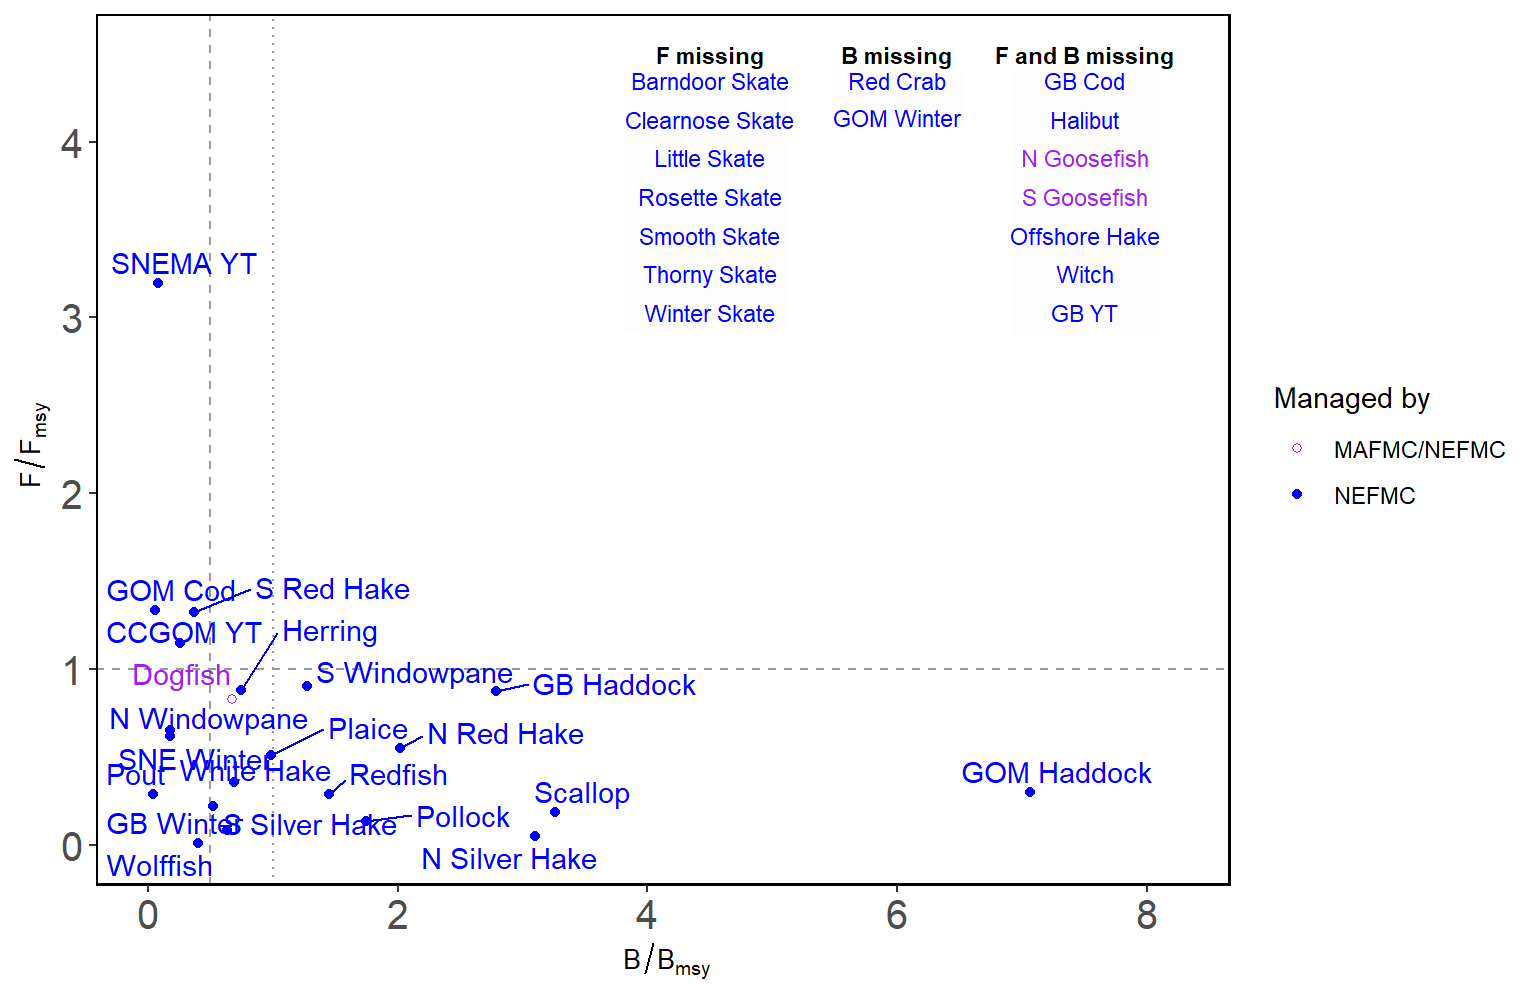
\includegraphics{C:/Users/kimberly.bastille/Desktop/tech-doc/imagesunnamed-chunk-60-1.pdf}
\caption{\label{fig:unnamed-chunk-60}Summary of single species status for
NEFMC and jointly managed stocks.}
\end{figure}

\chapter{Slopewater proportions}\label{slopewater-proportions}

\textbf{Description}: Percent total of water type observed in the deep
Northeast Channel (150-200 m water depth).

\textbf{Indicator category}: Published methods

\textbf{Found in}: State of the Ecosystem - Gulf of Maine \& Georges
Bank (2019)

\textbf{Contributors}: Paula Fratantoni,
\href{mailto:paula.fratantoni@noaa.gov}{\nolinkurl{paula.fratantoni@noaa.gov}};
David Mountain, NOAA Fisheries, retired.

\textbf{Data steward}: Kimberly Bastille,
\href{mailto:kimberly.bastille@noaa.gov}{\nolinkurl{kimberly.bastille@noaa.gov}}

\textbf{Point of contact}: Paula Fratantoni,
\href{mailto:paula.fratantoni@noaa.gov}{\nolinkurl{paula.fratantoni@noaa.gov}}

\textbf{Public availability statement}: Source data are publicly
available at
\url{ftp://ftp.nefsc.noaa.gov/pub/hydro/matlab_files/yearly} and in the
World Ocean Database housed at
\url{http://www.nodc.noaa.gov/OC5/SELECT/dbsearch/dbsearch.html} under
institute code 258

\section{Methods}\label{methods-27}

\subsection{Data sources}\label{data-sources-27}

The slope water composition index incorporates temperature and salinity
measurements collected on Northeast Fisheries Science Center surveys
between 1977-present within the geographic confines of the Northeast
Channel in the Gulf of Maine. Early measurements were made using water
samples collected primarily with Niskin bottles at discreet depths,
mechanical bathythermographs and expendable bathythermograph probes, but
by 1991 the CTD -- an acronym for conductivity temperature and depth --
became standard equipment on all NEFSC surveys.

\subsection{Data extraction}\label{data-extraction-22}

While all processed hydrographic data are archived in an Oracle database
(OCDBS), we work from Matlab-formatted files stored locally.

\subsection{Data analysis}\label{data-analysis-25}

Temperature and salinity measurements are examined to assess the
composition of the waters entering the Gulf of Maine through the
Northeast Channel. The analysis closely follows the methodology
described by D. G. Mountain
(\protect\hyperlink{ref-mountain2012}{2012}). This method assumes that
the waters flowing into the Northeast Channel between 150 and 200 meters
depth are composed of slope waters, originating offshore of the
continental shelf, and shelf waters, originating on the continental
shelf south of Nova Scotia.

For each survey in the hydrographic archive, ocean temperature and
salinity observations sampled in the area just inside the Northeast
Channel (bounded by 42.2-42.6\textdegree latitude north and
66-66.8\textdegree longitude west) and between 150 - 200 meters depth
are extracted and a volume-weighted average temperature and salinity is
calculated. The volume weighting is accomplished by apportioning the
area within the Northeast Channel polygon among the stations occupying
the region, based on inverse distance squared weighting. The result of
this calculation is a timeseries of volume-average temperature and
salinity having a temporal resolution that matches the survey frequency
in the database.

The average temperature and salinity observed at depth in the Northeast
Channel is assumed to be the product of mixing between three distinct
sources having the following temperature and salinity characteristics:
(1) Warm Slope Water (T=10 \textdegree C, S=35), (2) Labrador Slope
Water (T=6 \textdegree C, S=34.7) and (3) Scotian Shelf Water (T=2
\textdegree C, S=32). As described by D. G. Mountain
(\protect\hyperlink{ref-mountain2012}{2012}), the relative proportion of
each source is determined via a rudimentary 3-point mixing algorithm. On
a temperature-salinity diagram, lines connecting the T-S coordinates for
these three sources form a triangle, the sides of which represent mixing
lines between the sources. A water sample that is a mixture of two
sources will have a temperature and salinity that falls somewhere along
the line connecting the two sources on the temperature-salinity diagram.
Observations of temperature and salinity collected within the Northeast
Channel would be expected to fall within the triangle if the water
sampled is a mixture of the three sources. Simple geometry allows us to
calculate the relative proportion of each source in a given measurement.
As an example, a line drawn from the T-S point representing shelf water
through an observed T-S in the center of the triangle will intersect the
opposite side of the triangle (the mixing line connecting the
coordinates of the two slope water sources). This intersecting T-S value
may then be used to calculate the relative proportions (percentage) of
the two slope water sources. Using this method, the percentage of
Labrador slope water and Warm slope water are determined for the
timeseries of volume-average temperature and salinity.

It should be noted that our method assumes that the temperature and
salinity properties associated with the source watermasses are constant.
In reality, these may vary from year to year, modified by atmospheric
forcing, mixing and/or advective processes. Likewise, other sources are
periodically introduced into the Northeast Channel, including intrusions
of Gulf Stream water flowing into the Gulf of Maine and modified shelf
water flowing out of the Gulf of Maine along the flank of Georges Bank.
These sources are not explicitely considered in the 3-point mixing
algorithm and may introduce errors in the proportional estimates.

\subsection{Data processing}\label{data-processing-17}

Source data were formatted for inclusion in the ecodata R package using
the following R code.

\begin{Shaded}
\begin{Highlighting}[]
\CommentTok{# Process slopewater proportion time series}
\CommentTok{# }
\CommentTok{# Slopewater proportions give the percent total of water type observed in}
\CommentTok{# the deep Northeast Channel (150-200 m depth). }
\CommentTok{# }
\CommentTok{# Raw data fields correspond to year, water mass flavor (WSW = Warm Slope Water, LSLW = Labrador Slope Water),}
\CommentTok{# and proportion of total expressed as a percentage. }


\KeywordTok{library}\NormalTok{(dplyr)}
\KeywordTok{library}\NormalTok{(tidyr)}

\CommentTok{#Get raw}
\NormalTok{raw.dir <-}\StringTok{ }\NormalTok{here}\OperatorTok{::}\KeywordTok{here}\NormalTok{(}\StringTok{"data-raw"}\NormalTok{) }\CommentTok{#input raw}

\NormalTok{get_slopewater <-}\StringTok{ }\ControlFlowTok{function}\NormalTok{(}\DataTypeTok{save_clean =}\NormalTok{ F)\{}
  
\NormalTok{  d <-}\StringTok{ }\KeywordTok{read.csv}\NormalTok{(}\KeywordTok{file.path}\NormalTok{(raw.dir,}\StringTok{"slopewater_proportions.csv"}\NormalTok{))}
  
\NormalTok{  slopewater <-}\StringTok{ }\NormalTok{d }\OperatorTok
\StringTok{    }\NormalTok{dplyr}\OperatorTok{::}\KeywordTok{rename}\NormalTok{(}\DataTypeTok{Time =}\NormalTok{ year, }\DataTypeTok{Var =}\NormalTok{ water.mass.flavor, }\DataTypeTok{Value =}\NormalTok{ prop) }\OperatorTok\StringTok{ }
\StringTok{    }\KeywordTok{mutate}\NormalTok{(}\DataTypeTok{EPU =} \StringTok{"GOM"}\NormalTok{, }\DataTypeTok{Units =} \StringTok{"unitless"}\NormalTok{, }\DataTypeTok{Var2 =} \StringTok{"proportion ne channel"}\NormalTok{) }\OperatorTok\StringTok{ }
\StringTok{    }\KeywordTok{unite}\NormalTok{(.,Var,}\KeywordTok{c}\NormalTok{(Var,Var2), }\DataTypeTok{sep =} \StringTok{" "}\NormalTok{) }\OperatorTok\StringTok{ }
\StringTok{    }\KeywordTok{as.data.frame}\NormalTok{()}
  
  \ControlFlowTok{if}\NormalTok{ (save_clean)\{}
\NormalTok{    usethis}\OperatorTok{::}\KeywordTok{use_data}\NormalTok{(slopewater, }\DataTypeTok{overwrite =}\NormalTok{ T)}
\NormalTok{  \} }\ControlFlowTok{else}\NormalTok{ \{}
    \KeywordTok{return}\NormalTok{(slopewater)}
\NormalTok{  \}}
  
\NormalTok{\}}
\end{Highlighting}
\end{Shaded}

\subsection{Plotting}\label{plotting-19}

\begin{Shaded}
\begin{Highlighting}[]
\NormalTok{sw.df <-}\StringTok{ }\NormalTok{slopewater }\OperatorTok\StringTok{ }
\StringTok{  }\KeywordTok{mutate}\NormalTok{(Var, }\DataTypeTok{Var =}\NormalTok{ plyr}\OperatorTok{::}\KeywordTok{mapvalues}\NormalTok{(Var, }\DataTypeTok{from =} \KeywordTok{c}\NormalTok{(}\StringTok{"WSW proportion ne channel"}\NormalTok{,}
                                                  \StringTok{"LSLW proportion ne channel"}\NormalTok{),}
                                    \DataTypeTok{to =} \KeywordTok{c}\NormalTok{(}\StringTok{"WSW"}\NormalTok{,}\StringTok{"LSLW"}\NormalTok{))) }\OperatorTok\StringTok{ }
\StringTok{  }\NormalTok{dplyr}\OperatorTok{::}\KeywordTok{rename}\NormalTok{(}\DataTypeTok{Origin  =}\NormalTok{ Var) }\OperatorTok\StringTok{ }
\StringTok{  }\KeywordTok{group_by}\NormalTok{(Origin) }\OperatorTok\StringTok{ }
\StringTok{  }\KeywordTok{mutate}\NormalTok{(}\DataTypeTok{hline =} \KeywordTok{mean}\NormalTok{(Value)) }

\NormalTok{sw.df}\OperatorTok{$}\NormalTok{Origin <-}\StringTok{ }\KeywordTok{factor}\NormalTok{(sw.df}\OperatorTok{$}\NormalTok{Origin, }\DataTypeTok{levels =} \KeywordTok{c}\NormalTok{(}\StringTok{"WSW"}\NormalTok{,}\StringTok{"LSLW"}\NormalTok{))}

\KeywordTok{ggplot}\NormalTok{(}\DataTypeTok{data =}\NormalTok{ sw.df) }\OperatorTok{+}
\StringTok{  }\KeywordTok{geom_line}\NormalTok{(}\KeywordTok{aes}\NormalTok{(}\DataTypeTok{x =}\NormalTok{ Time, }\DataTypeTok{y =}\NormalTok{ Value, }\DataTypeTok{color =}\NormalTok{ Origin))}\OperatorTok{+}
\StringTok{  }\KeywordTok{geom_point}\NormalTok{(}\KeywordTok{aes}\NormalTok{(}\DataTypeTok{x =}\NormalTok{ Time, }\DataTypeTok{y =}\NormalTok{ Value, }\DataTypeTok{color =}\NormalTok{ Origin)) }\OperatorTok{+}
\StringTok{  }\KeywordTok{ylab}\NormalTok{(}\StringTok{"Percent of Total Slopewater"}\NormalTok{) }\OperatorTok{+}
\StringTok{  }\KeywordTok{ggtitle}\NormalTok{(}\StringTok{"Slopewater Proportions in NE Channel"}\NormalTok{)}\OperatorTok{+}
\StringTok{    }\KeywordTok{scale_x_continuous}\NormalTok{(}\DataTypeTok{expand =} \KeywordTok{c}\NormalTok{(}\FloatTok{0.01}\NormalTok{, }\FloatTok{0.01}\NormalTok{))}\OperatorTok{+}
\StringTok{      }\KeywordTok{geom_hline}\NormalTok{(}\KeywordTok{aes}\NormalTok{(}\DataTypeTok{yintercept =}\NormalTok{ hline,}
                     \DataTypeTok{color =}\NormalTok{ Origin),}
           \DataTypeTok{size =}\NormalTok{ hline.size,}
           \DataTypeTok{alpha =}\NormalTok{ hline.alpha,}
           \DataTypeTok{linetype =}\NormalTok{ hline.lty)}\OperatorTok{+}
\StringTok{  }\KeywordTok{theme_ts}\NormalTok{() }\OperatorTok{+}
\StringTok{  }\KeywordTok{theme}\NormalTok{(}\DataTypeTok{strip.text=}\KeywordTok{element_text}\NormalTok{(}\DataTypeTok{hjust=}\DecValTok{0}\NormalTok{,}
                                \DataTypeTok{face =} \StringTok{"italic"}\NormalTok{))}
\end{Highlighting}
\end{Shaded}

\begin{figure}

{\centering 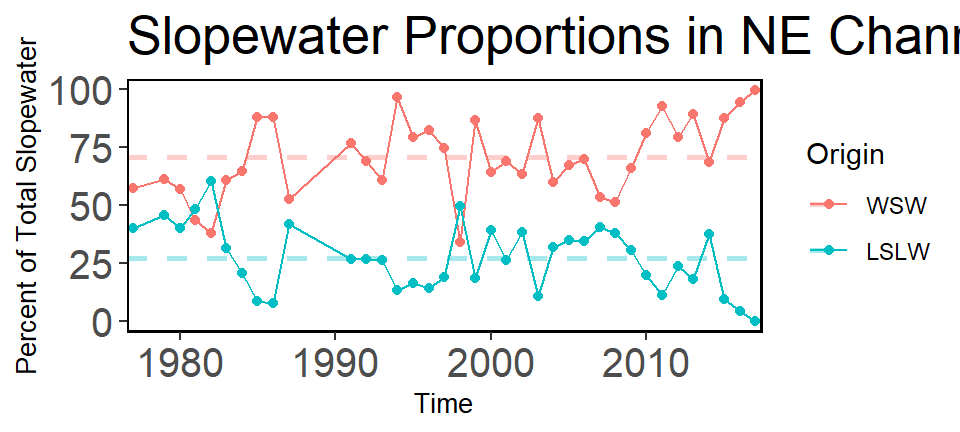
\includegraphics{C:/Users/kimberly.bastille/Desktop/tech-doc/imagesunnamed-chunk-63-1} 

}

\caption{Proportion of warm slope water (WSW) and Labrador slope water (LSLW) entering the GOM through the Northeast Channel.}\label{fig:unnamed-chunk-63}
\end{figure}

\chapter{Species Density Estimates}\label{species-density-estimates}

\textbf{Description}: Current and Historical Species Distributions

\textbf{Found in}: State of the Ecosystem - Gulf of Maine \& Georges
Bank (2017, 2018), State of the Ecosystem - Mid-Atlantic (2017, 2018)

\textbf{Indicator category}: Database pull; Database pull with analysis

\textbf{Contributor}: Kevin Friedland

\textbf{Data steward}: Kevin Friedland

\textbf{Point of contact}: Kevin Friedland,
\href{mailto:kevin.friedland@noaa.gov}{\nolinkurl{kevin.friedland@noaa.gov}}

\textbf{Public availability statement}: Source data are publicly
available.

\section{Methods}\label{methods-28}

We used kernel density plots to depict shifts in species' distributions
over time. These figures characterize the probability of a species
occurring in a given area based on NEFSC Bottom Trawl Survey data.
Kernel density estimates (KDEs) of distributions are shown for the
period of 1970-1979 (shaded blue) and most recent three years of survey
data (shaded red) (e.g.~Figure \ref{fig:kde-fig}). Results are typically
visualized for spring and fall bottom trawl surveys seperately.

Three probability levels (25\%, 50\%, 75\%) are shown for each time
period, where the 25\% region depicts the core area of the distribution
and the 75\% region shows the area occupied more broadly by the species.
A wide array of KDEs for many ecologically and economically important
species on the Northeast US Continental Shelf are available
\href{https://www.nefsc.noaa.gov/ecosys/current-conditions/kernel-density.html}{here}.

\subsection{Data sources}\label{data-sources-28}

Current and historical species distributions are based on the NEFSC
Bottom Trawl Survey data (aka \protect\hyperlink{survdat}{``Survdat''})
and depth strata. Strata are available as shapefiles that can be
downloaded
\href{https://github.com/NOAA-EDAB/tech-doc/tree/master/gis}{here}
(listed as ``strata.shp'').

\subsection{Data analysis}\label{data-analysis-26}

\begin{Shaded}
\begin{Highlighting}[]
\KeywordTok{library}\NormalTok{(ecodata)}
\KeywordTok{library}\NormalTok{(maps)}
\KeywordTok{library}\NormalTok{(mapdata)}
\KeywordTok{library}\NormalTok{(ks)}
\KeywordTok{library}\NormalTok{(marmap)}
\KeywordTok{library}\NormalTok{(raster)}
\KeywordTok{library}\NormalTok{(geosphere)}
\KeywordTok{library}\NormalTok{(dplyr)}

\CommentTok{#  plot ks plots}

\CommentTok{#----STUFF TO SET-----------------}
\NormalTok{data.dir <-}\StringTok{ }\NormalTok{here}\OperatorTok{::}\KeywordTok{here}\NormalTok{(}\StringTok{"data"}\NormalTok{)}
\NormalTok{gis.dir <-}\StringTok{ }\NormalTok{here}\OperatorTok{::}\KeywordTok{here}\NormalTok{(}\StringTok{"gis"}\NormalTok{)}

\CommentTok{# Gives most recent period. 2015-2019 input is 2016-2018 data}
\NormalTok{rminyr <-}\StringTok{ }\DecValTok{2015}
\NormalTok{rmaxyr <-}\StringTok{ }\DecValTok{2019}

\CommentTok{# tlevel is density of color for KD contours areas}
\NormalTok{tlevel=}\DecValTok{75}  \CommentTok{# move later}
\NormalTok{color_b=}\StringTok{"blue"}
\NormalTok{color_r=}\StringTok{"orange3"}
\NormalTok{color_r=}\StringTok{"tomato3"}

\CommentTok{# Code to read in strata and compute areas. Or read from cache.}

\CommentTok{# readin in strata.shp and compute areas of strata}
\CommentTok{# TrawlStrata <- raster::shapefile(file.path(gis.dir,"BTS_Strata.shp"))}
\CommentTok{# AREA <- geosphere::areaPolygon(TrawlStrata, r=6371000)/10^6}

\CommentTok{# for array of strata and area and make into dataframe}
\CommentTok{# stratareas <- cbind(TrawlStrata@data$STRATA, AREA)}
\CommentTok{# colnames(stratareas) <- c("STRATA","AREA")}
\CommentTok{# stratareas <- data.frame(stratareas)}
\KeywordTok{load}\NormalTok{(}\KeywordTok{file.path}\NormalTok{(data.dir, }\StringTok{"StratAreas.Rdata"}\NormalTok{))}

\CommentTok{# Query bathymetry or load from cache}
\CommentTok{# getNOAA.bathy(lon1 = -77, lon2 = -65, lat1 = 35, lat2 = 45,}
\CommentTok{#               resolution = 10) -> nesbath}
\KeywordTok{load}\NormalTok{(}\KeywordTok{file.path}\NormalTok{(data.dir, }\StringTok{"nesbath.Rdata"}\NormalTok{))}

\CommentTok{#Load raw survey data}
\KeywordTok{load}\NormalTok{(}\KeywordTok{file.path}\NormalTok{(data.dir, }\StringTok{"Survdat.RData"}\NormalTok{))}

\CommentTok{# MUST run addTrans function}
\CommentTok{# color transparency}
\NormalTok{addTrans <-}\StringTok{ }\ControlFlowTok{function}\NormalTok{(color,trans)\{}
  \CommentTok{# This function adds transparancy to a color.}
  \CommentTok{# Define transparancy with an integer between 0 and 255}
  \CommentTok{# 0 being fully transparant and 255 being fully visable}
  \CommentTok{# Works with either color and trans a vector of equal length,}
  \CommentTok{# or one of the two of length 1.}
  
  \ControlFlowTok{if}\NormalTok{ (}\KeywordTok{length}\NormalTok{(color)}\OperatorTok{!=}\KeywordTok{length}\NormalTok{(trans)}\OperatorTok{&!}\KeywordTok{any}\NormalTok{(}\KeywordTok{c}\NormalTok{(}\KeywordTok{length}\NormalTok{(color),}\KeywordTok{length}\NormalTok{(trans))}\OperatorTok{==}\DecValTok{1}\NormalTok{)) }\KeywordTok{stop}\NormalTok{(}\StringTok{"Vector lengths not correct"}\NormalTok{)}
  \ControlFlowTok{if}\NormalTok{ (}\KeywordTok{length}\NormalTok{(color)}\OperatorTok{==}\DecValTok{1} \OperatorTok{&}\StringTok{ }\KeywordTok{length}\NormalTok{(trans)}\OperatorTok{>}\DecValTok{1}\NormalTok{) color <-}\StringTok{ }\KeywordTok{rep}\NormalTok{(color,}\KeywordTok{length}\NormalTok{(trans))}
  \ControlFlowTok{if}\NormalTok{ (}\KeywordTok{length}\NormalTok{(trans)}\OperatorTok{==}\DecValTok{1} \OperatorTok{&}\StringTok{ }\KeywordTok{length}\NormalTok{(color)}\OperatorTok{>}\DecValTok{1}\NormalTok{) trans <-}\StringTok{ }\KeywordTok{rep}\NormalTok{(trans,}\KeywordTok{length}\NormalTok{(color))}
  
\NormalTok{  num2hex <-}\StringTok{ }\ControlFlowTok{function}\NormalTok{(x)}
\NormalTok{  \{}
\NormalTok{    hex <-}\StringTok{ }\KeywordTok{unlist}\NormalTok{(}\KeywordTok{strsplit}\NormalTok{(}\StringTok{"0123456789ABCDEF"}\NormalTok{,}\DataTypeTok{split=}\StringTok{""}\NormalTok{))}
    \KeywordTok{return}\NormalTok{(}\KeywordTok{paste}\NormalTok{(hex[(x}\OperatorTok{-}\NormalTok{x}\OperatorTok\DecValTok{16}\NormalTok{)}\OperatorTok{/}\DecValTok{16}\OperatorTok{+}\DecValTok{1}\NormalTok{],hex[x}\OperatorTok\DecValTok{16}\OperatorTok{+}\DecValTok{1}\NormalTok{],}\DataTypeTok{sep=}\StringTok{""}\NormalTok{))}
\NormalTok{  \}}
\NormalTok{  rgb <-}\StringTok{ }\KeywordTok{rbind}\NormalTok{(}\KeywordTok{col2rgb}\NormalTok{(color),trans)}
\NormalTok{  res <-}\StringTok{ }\KeywordTok{paste}\NormalTok{(}\StringTok{"#"}\NormalTok{,}\KeywordTok{apply}\NormalTok{(}\KeywordTok{apply}\NormalTok{(rgb,}\DecValTok{2}\NormalTok{,num2hex),}\DecValTok{2}\NormalTok{,paste,}\DataTypeTok{collapse=}\StringTok{""}\NormalTok{),}\DataTypeTok{sep=}\StringTok{""}\NormalTok{)}
  \KeywordTok{return}\NormalTok{(res)}
\NormalTok{\}}

\NormalTok{plot_kd <-}\StringTok{ }\ControlFlowTok{function}\NormalTok{(species, season, exclude_years)\{}

  \CommentTok{# stata to use}
  \CommentTok{# offshore strata to use}
\NormalTok{  CoreOffshoreStrata <-}\StringTok{ }\KeywordTok{c}\NormalTok{(}\KeywordTok{seq}\NormalTok{(}\DecValTok{1010}\NormalTok{,}\DecValTok{1300}\NormalTok{,}\DecValTok{10}\NormalTok{),}\DecValTok{1340}\NormalTok{, }\KeywordTok{seq}\NormalTok{(}\DecValTok{1360}\NormalTok{,}\DecValTok{1400}\NormalTok{,}\DecValTok{10}\NormalTok{),}\KeywordTok{seq}\NormalTok{(}\DecValTok{1610}\NormalTok{,}\DecValTok{1760}\NormalTok{,}\DecValTok{10}\NormalTok{))}
  
  \CommentTok{# inshore strata to use, still sampled by Bigelow}
\NormalTok{  CoreInshore73to12 <-}\StringTok{ }\KeywordTok{c}\NormalTok{(}\DecValTok{3020}\NormalTok{, }\DecValTok{3050}\NormalTok{, }\DecValTok{3080}\NormalTok{ ,}\DecValTok{3110}\NormalTok{ ,}\DecValTok{3140}\NormalTok{ ,}\DecValTok{3170}\NormalTok{, }\DecValTok{3200}\NormalTok{, }\DecValTok{3230}\NormalTok{,}
                         \DecValTok{3260}\NormalTok{, }\DecValTok{3290}\NormalTok{, }\DecValTok{3320}\NormalTok{, }\DecValTok{3350}\NormalTok{ ,}\DecValTok{3380}\NormalTok{, }\DecValTok{3410}\NormalTok{ ,}\DecValTok{3440}\NormalTok{)}
  \CommentTok{# combine}
\NormalTok{  strata_used <-}\StringTok{ }\KeywordTok{c}\NormalTok{(CoreOffshoreStrata,CoreInshore73to12)}
  
\NormalTok{  survdat <-}\StringTok{ }\NormalTok{survdat }\OperatorTok
\StringTok{    }\NormalTok{dplyr}\OperatorTok{::}\KeywordTok{select}\NormalTok{(}\KeywordTok{c}\NormalTok{(CRUISE6,STATION,STRATUM,SVSPP,YEAR,}
\NormalTok{                    SEASON,LAT,LON,ABUNDANCE,BIOMASS)) }\OperatorTok\StringTok{ }
\StringTok{    }\KeywordTok{filter}\NormalTok{(SEASON }\OperatorTok{==}\StringTok{ }\NormalTok{season,}
\NormalTok{           STRATUM }\OperatorTok\StringTok{ }\NormalTok{strata_used) }\OperatorTok\StringTok{ }\CommentTok{# delete record form non-core strata and get unique records,}
\StringTok{    }\CommentTok{# should be one per species}
\StringTok{    }\KeywordTok{distinct}\NormalTok{() }\OperatorTok\StringTok{ }
\StringTok{    }\CommentTok{# add field with rounded BIOMASS scaler used to adjust distributions}
\StringTok{    }\KeywordTok{mutate}\NormalTok{(}\DataTypeTok{LOGBIO =} \KeywordTok{round}\NormalTok{(}\KeywordTok{log10}\NormalTok{(BIOMASS }\OperatorTok{*}\StringTok{ }\DecValTok{10}\OperatorTok{+}\DecValTok{10}\NormalTok{)))}

  \CommentTok{# trim the data....to prepare to find stations only}
\NormalTok{  survdat_stations <-}\StringTok{ }\NormalTok{survdat }\OperatorTok\StringTok{ }
\StringTok{    }\NormalTok{dplyr}\OperatorTok{::}\KeywordTok{select}\NormalTok{(CRUISE6, STATION, STRATUM, YEAR) }\OperatorTok\StringTok{ }
\StringTok{    }\KeywordTok{distinct}\NormalTok{()}
  
  \CommentTok{# make table of strata by year}
\NormalTok{  numtowsstratyr <-}\StringTok{ }\KeywordTok{table}\NormalTok{(survdat_stations}\OperatorTok{$}\NormalTok{STRATUM,survdat_stations}\OperatorTok{$}\NormalTok{YEAR)}
  
  \CommentTok{# find records to keep based on core strata}
\NormalTok{  rectokeep <-}\StringTok{ }\NormalTok{stratareas}\OperatorTok{$}\NormalTok{STRATA }\OperatorTok\StringTok{ }\NormalTok{strata_used}
  
  \CommentTok{# add rec to keep to survdat}
\NormalTok{  stratareas <-}\StringTok{ }\KeywordTok{cbind}\NormalTok{(stratareas,rectokeep)}
  
  \CommentTok{# delete record form non-core strata}
\NormalTok{  stratareas_usedonly <-}\StringTok{ }\NormalTok{stratareas[}\OperatorTok{!}\NormalTok{stratareas}\OperatorTok{$}\NormalTok{rectokeep}\OperatorTok{==}\StringTok{"FALSE"}\NormalTok{,]}
    
\NormalTok{  areapertow=numtowsstratyr}
  
  \CommentTok{#compute area covered per tow per strata per year}
  \ControlFlowTok{for}\NormalTok{(i }\ControlFlowTok{in} \DecValTok{1}\OperatorTok{:}\DecValTok{50}\NormalTok{)\{}
\NormalTok{  areapertow[,i]=stratareas_usedonly}\OperatorTok{$}\NormalTok{AREA}\OperatorTok{/}\NormalTok{numtowsstratyr[,i]}
\NormalTok{  \}}
  
  \CommentTok{# change inf to NA and round and out in DF}
\NormalTok{  areapertow[][}\KeywordTok{is.infinite}\NormalTok{(areapertow[])]=}\OtherTok{NA}
\NormalTok{  areapertow=}\KeywordTok{round}\NormalTok{(areapertow)}
\NormalTok{  areapertow=}\KeywordTok{data.frame}\NormalTok{(areapertow)}
  \KeywordTok{colnames}\NormalTok{(areapertow) <-}\StringTok{ }\KeywordTok{c}\NormalTok{(}\StringTok{"STRATUM"}\NormalTok{,}\StringTok{"YEAR"}\NormalTok{,}\StringTok{"AREAWT"}\NormalTok{)}
\NormalTok{  areapertow}\OperatorTok{$}\NormalTok{STRATUM <-}\StringTok{ }\KeywordTok{as.numeric}\NormalTok{(}\KeywordTok{as.character}\NormalTok{(areapertow}\OperatorTok{$}\NormalTok{STRATUM))}
\NormalTok{  areapertow}\OperatorTok{$}\NormalTok{YEAR <-}\StringTok{ }\KeywordTok{as.numeric}\NormalTok{(}\KeywordTok{as.character}\NormalTok{(areapertow}\OperatorTok{$}\NormalTok{YEAR))}
    
\NormalTok{  survdat <-}\StringTok{ }\NormalTok{survdat }\OperatorTok\StringTok{ }
\StringTok{    }\KeywordTok{inner_join}\NormalTok{(.,areapertow, }\DataTypeTok{by=} \KeywordTok{c}\NormalTok{(}\StringTok{"STRATUM"}\NormalTok{,}\StringTok{"YEAR"}\NormalTok{)) }\OperatorTok\StringTok{ }
\StringTok{    }\NormalTok{dplyr}\OperatorTok{::}\KeywordTok{rename}\NormalTok{(}\DataTypeTok{AREAPERTOW =}\NormalTok{ AREAWT)}
  
  \CommentTok{# add col to survdat for PLOTWT}
\NormalTok{  survdat}\OperatorTok{$}\NormalTok{PLOTWT <-}\StringTok{ }\OtherTok{NA}
\NormalTok{  survdat}\OperatorTok{$}\NormalTok{PLOTWT <-}\StringTok{ }\KeywordTok{ceiling}\NormalTok{(survdat}\OperatorTok{$}\NormalTok{AREAPERTOW}\OperatorTok{/}\DecValTok{1000}\OperatorTok{*}\NormalTok{survdat}\OperatorTok{$}\NormalTok{LOGBIO}\OperatorTok{/}\DecValTok{9}\NormalTok{)}
  
  \ControlFlowTok{if}\NormalTok{ (}\OperatorTok{!}\KeywordTok{is.null}\NormalTok{(exclude_years))\{}
\NormalTok{    sdat <-}\StringTok{ }\NormalTok{survdat }\OperatorTok\StringTok{ }\KeywordTok{filter}\NormalTok{(}\OperatorTok{!}\NormalTok{YEAR }\OperatorTok\StringTok{ }\NormalTok{exclude_years)}
\NormalTok{  \} }\ControlFlowTok{else}\NormalTok{ \{}
\NormalTok{    sdat <-}\StringTok{ }\NormalTok{survdat}
\NormalTok{  \}}
  
  \CommentTok{# read species list}
\NormalTok{  sps <-}\StringTok{ }\NormalTok{ecodata}\OperatorTok{::}\NormalTok{species_groupings }\OperatorTok\StringTok{ }\KeywordTok{filter}\NormalTok{(}\OperatorTok{!}\KeywordTok{is.na}\NormalTok{(SVSPP)) }\OperatorTok\StringTok{ }\NormalTok{dplyr}\OperatorTok{::}\KeywordTok{select}\NormalTok{(COMNAME, SVSPP)}
\NormalTok{  sps <-}\StringTok{ }\NormalTok{sps[}\OperatorTok{!}\KeywordTok{duplicated}\NormalTok{(sps),]}
\NormalTok{  numsps <-}\StringTok{ }\KeywordTok{nrow}\NormalTok{(sps)}
  
  \CommentTok{# graph par}
  \KeywordTok{par}\NormalTok{(}\DataTypeTok{mar =} \KeywordTok{c}\NormalTok{(}\DecValTok{0}\NormalTok{,}\DecValTok{0}\NormalTok{,}\DecValTok{0}\NormalTok{,}\DecValTok{0}\NormalTok{))}
  \KeywordTok{par}\NormalTok{(}\DataTypeTok{oma =} \KeywordTok{c}\NormalTok{(}\DecValTok{0}\NormalTok{,}\DecValTok{0}\NormalTok{,}\DecValTok{0}\NormalTok{,}\DecValTok{0}\NormalTok{))}
  
  \CommentTok{# index 1:numsps, or by species record number for one species, i.e.25:25}
\NormalTok{  tspe <-}\StringTok{ }\NormalTok{sps }\OperatorTok\StringTok{ }\KeywordTok{filter}\NormalTok{(COMNAME }\OperatorTok{==}\StringTok{ }\NormalTok{species)}

  \CommentTok{# start map}
  \KeywordTok{map}\NormalTok{(}\StringTok{"worldHires"}\NormalTok{, }\DataTypeTok{xlim=}\KeywordTok{c}\NormalTok{(}\OperatorTok{-}\DecValTok{77}\NormalTok{,}\OperatorTok{-}\DecValTok{65}\NormalTok{),}\DataTypeTok{ylim=}\KeywordTok{c}\NormalTok{(}\DecValTok{35}\NormalTok{,}\DecValTok{45}\NormalTok{), }\DataTypeTok{fill=}\NormalTok{T,}\DataTypeTok{border=}\DecValTok{0}\NormalTok{,}\DataTypeTok{col=}\StringTok{"gray"}\NormalTok{)}
  \KeywordTok{map.axes}\NormalTok{()}

  \KeywordTok{plot}\NormalTok{(nesbath,}\DataTypeTok{deep=}\OperatorTok{-}\DecValTok{200}\NormalTok{, }\DataTypeTok{shallow=}\OperatorTok{-}\DecValTok{200}\NormalTok{, }\DataTypeTok{step=}\DecValTok{1}\NormalTok{,}\DataTypeTok{add=}\NormalTok{T,}\DataTypeTok{lwd=}\DecValTok{1}\NormalTok{,}\DataTypeTok{col=}\StringTok{"gray50"}\NormalTok{,}\DataTypeTok{lty=}\DecValTok{2}\NormalTok{)}


  \CommentTok{# for base period, 1970 to 1979, find call lons for species and by biomass weighting}
\NormalTok{  minyr=}\DecValTok{1969}\NormalTok{;maxyr=}\DecValTok{1980}
\NormalTok{  clons1 =}\StringTok{ }\NormalTok{sdat}\OperatorTok{$}\NormalTok{LON[(sdat}\OperatorTok{$}\NormalTok{YEAR}\OperatorTok{>}\NormalTok{minyr }\OperatorTok{&}\StringTok{ }\NormalTok{sdat}\OperatorTok{$}\NormalTok{YEAR}\OperatorTok{<}\NormalTok{maxyr }\OperatorTok{&}\StringTok{ }\NormalTok{sdat}\OperatorTok{$}\NormalTok{SVSPP}\OperatorTok{==}\NormalTok{tspe}\OperatorTok{$}\NormalTok{SVSPP }\OperatorTok{&}\StringTok{ }\NormalTok{sdat}\OperatorTok{$}\NormalTok{PLOTWT }\OperatorTok{==}\DecValTok{1}\NormalTok{)]}
\NormalTok{  clons2 =}\StringTok{ }\NormalTok{sdat}\OperatorTok{$}\NormalTok{LON[(sdat}\OperatorTok{$}\NormalTok{YEAR}\OperatorTok{>}\NormalTok{minyr }\OperatorTok{&}\StringTok{ }\NormalTok{sdat}\OperatorTok{$}\NormalTok{YEAR}\OperatorTok{<}\NormalTok{maxyr }\OperatorTok{&}\StringTok{ }\NormalTok{sdat}\OperatorTok{$}\NormalTok{SVSPP}\OperatorTok{==}\NormalTok{tspe}\OperatorTok{$}\NormalTok{SVSPP }\OperatorTok{&}\StringTok{ }\NormalTok{sdat}\OperatorTok{$}\NormalTok{PLOTWT }\OperatorTok{==}\DecValTok{2}\NormalTok{)]}
\NormalTok{  clons3 =}\StringTok{ }\NormalTok{sdat}\OperatorTok{$}\NormalTok{LON[(sdat}\OperatorTok{$}\NormalTok{YEAR}\OperatorTok{>}\NormalTok{minyr }\OperatorTok{&}\StringTok{ }\NormalTok{sdat}\OperatorTok{$}\NormalTok{YEAR}\OperatorTok{<}\NormalTok{maxyr }\OperatorTok{&}\StringTok{ }\NormalTok{sdat}\OperatorTok{$}\NormalTok{SVSPP}\OperatorTok{==}\NormalTok{tspe}\OperatorTok{$}\NormalTok{SVSPP }\OperatorTok{&}\StringTok{ }\NormalTok{sdat}\OperatorTok{$}\NormalTok{PLOTWT }\OperatorTok{==}\DecValTok{3}\NormalTok{)]}
\NormalTok{  clons4 =}\StringTok{ }\NormalTok{sdat}\OperatorTok{$}\NormalTok{LON[(sdat}\OperatorTok{$}\NormalTok{YEAR}\OperatorTok{>}\NormalTok{minyr }\OperatorTok{&}\StringTok{ }\NormalTok{sdat}\OperatorTok{$}\NormalTok{YEAR}\OperatorTok{<}\NormalTok{maxyr }\OperatorTok{&}\StringTok{ }\NormalTok{sdat}\OperatorTok{$}\NormalTok{SVSPP}\OperatorTok{==}\NormalTok{tspe}\OperatorTok{$}\NormalTok{SVSPP }\OperatorTok{&}\StringTok{ }\NormalTok{sdat}\OperatorTok{$}\NormalTok{PLOTWT }\OperatorTok{==}\DecValTok{4}\NormalTok{)]}
\NormalTok{  clons5 =}\StringTok{ }\NormalTok{sdat}\OperatorTok{$}\NormalTok{LON[(sdat}\OperatorTok{$}\NormalTok{YEAR}\OperatorTok{>}\NormalTok{minyr }\OperatorTok{&}\StringTok{ }\NormalTok{sdat}\OperatorTok{$}\NormalTok{YEAR}\OperatorTok{<}\NormalTok{maxyr }\OperatorTok{&}\StringTok{ }\NormalTok{sdat}\OperatorTok{$}\NormalTok{SVSPP}\OperatorTok{==}\NormalTok{tspe}\OperatorTok{$}\NormalTok{SVSPP }\OperatorTok{&}\StringTok{ }\NormalTok{sdat}\OperatorTok{$}\NormalTok{PLOTWT }\OperatorTok{==}\DecValTok{4}\NormalTok{)]}
  
  \CommentTok{# get rid of missings, KS does not like}
\NormalTok{  clons1 <-}\StringTok{ }\KeywordTok{na.omit}\NormalTok{(clons1)}
\NormalTok{  clons2 <-}\StringTok{ }\KeywordTok{na.omit}\NormalTok{(clons2)}
\NormalTok{  clons3 <-}\StringTok{ }\KeywordTok{na.omit}\NormalTok{(clons3)}
\NormalTok{  clons4 <-}\StringTok{ }\KeywordTok{na.omit}\NormalTok{(clons4)}
\NormalTok{  clons5 <-}\StringTok{ }\KeywordTok{na.omit}\NormalTok{(clons5)}
  
  \CommentTok{# accumulate all lons, repeating for weighting }
\NormalTok{  clons=}\KeywordTok{c}\NormalTok{(clons1,clons2,clons2,clons3,clons3,clons3,clons4,clons4,clons4,clons4,}
\NormalTok{          clons5,clons5,clons5,clons5,clons5)}

  \CommentTok{# same for lats}
\NormalTok{  clats1 =}\StringTok{ }\NormalTok{sdat}\OperatorTok{$}\NormalTok{LAT[(sdat}\OperatorTok{$}\NormalTok{YEAR}\OperatorTok{>}\NormalTok{minyr }\OperatorTok{&}\StringTok{ }\NormalTok{sdat}\OperatorTok{$}\NormalTok{YEAR}\OperatorTok{<}\NormalTok{maxyr }\OperatorTok{&}\StringTok{ }\NormalTok{sdat}\OperatorTok{$}\NormalTok{SVSPP}\OperatorTok{==}\NormalTok{tspe}\OperatorTok{$}\NormalTok{SVSPP }\OperatorTok{&}\StringTok{ }\NormalTok{sdat}\OperatorTok{$}\NormalTok{PLOTWT }\OperatorTok{==}\DecValTok{1}\NormalTok{)]}
\NormalTok{  clats2 =}\StringTok{ }\NormalTok{sdat}\OperatorTok{$}\NormalTok{LAT[(sdat}\OperatorTok{$}\NormalTok{YEAR}\OperatorTok{>}\NormalTok{minyr }\OperatorTok{&}\StringTok{ }\NormalTok{sdat}\OperatorTok{$}\NormalTok{YEAR}\OperatorTok{<}\NormalTok{maxyr }\OperatorTok{&}\StringTok{ }\NormalTok{sdat}\OperatorTok{$}\NormalTok{SVSPP}\OperatorTok{==}\NormalTok{tspe}\OperatorTok{$}\NormalTok{SVSPP }\OperatorTok{&}\StringTok{ }\NormalTok{sdat}\OperatorTok{$}\NormalTok{PLOTWT }\OperatorTok{==}\DecValTok{2}\NormalTok{)]}
\NormalTok{  clats3 =}\StringTok{ }\NormalTok{sdat}\OperatorTok{$}\NormalTok{LAT[(sdat}\OperatorTok{$}\NormalTok{YEAR}\OperatorTok{>}\NormalTok{minyr }\OperatorTok{&}\StringTok{ }\NormalTok{sdat}\OperatorTok{$}\NormalTok{YEAR}\OperatorTok{<}\NormalTok{maxyr }\OperatorTok{&}\StringTok{ }\NormalTok{sdat}\OperatorTok{$}\NormalTok{SVSPP}\OperatorTok{==}\NormalTok{tspe}\OperatorTok{$}\NormalTok{SVSPP }\OperatorTok{&}\StringTok{ }\NormalTok{sdat}\OperatorTok{$}\NormalTok{PLOTWT }\OperatorTok{==}\DecValTok{3}\NormalTok{)]}
\NormalTok{  clats4 =}\StringTok{ }\NormalTok{sdat}\OperatorTok{$}\NormalTok{LAT[(sdat}\OperatorTok{$}\NormalTok{YEAR}\OperatorTok{>}\NormalTok{minyr }\OperatorTok{&}\StringTok{ }\NormalTok{sdat}\OperatorTok{$}\NormalTok{YEAR}\OperatorTok{<}\NormalTok{maxyr }\OperatorTok{&}\StringTok{ }\NormalTok{sdat}\OperatorTok{$}\NormalTok{SVSPP}\OperatorTok{==}\NormalTok{tspe}\OperatorTok{$}\NormalTok{SVSPP }\OperatorTok{&}\StringTok{ }\NormalTok{sdat}\OperatorTok{$}\NormalTok{PLOTWT }\OperatorTok{==}\DecValTok{4}\NormalTok{)]}
\NormalTok{  clats5 =}\StringTok{ }\NormalTok{sdat}\OperatorTok{$}\NormalTok{LAT[(sdat}\OperatorTok{$}\NormalTok{YEAR}\OperatorTok{>}\NormalTok{minyr }\OperatorTok{&}\StringTok{ }\NormalTok{sdat}\OperatorTok{$}\NormalTok{YEAR}\OperatorTok{<}\NormalTok{maxyr }\OperatorTok{&}\StringTok{ }\NormalTok{sdat}\OperatorTok{$}\NormalTok{SVSPP}\OperatorTok{==}\NormalTok{tspe}\OperatorTok{$}\NormalTok{SVSPP }\OperatorTok{&}\StringTok{ }\NormalTok{sdat}\OperatorTok{$}\NormalTok{PLOTWT }\OperatorTok{==}\DecValTok{5}\NormalTok{)]}
\NormalTok{  clats1 <-}\StringTok{ }\KeywordTok{na.omit}\NormalTok{(clats1)}
\NormalTok{  clats2 <-}\StringTok{ }\KeywordTok{na.omit}\NormalTok{(clats2)}
\NormalTok{  clats3 <-}\StringTok{ }\KeywordTok{na.omit}\NormalTok{(clats3)}
\NormalTok{  clats4 <-}\StringTok{ }\KeywordTok{na.omit}\NormalTok{(clats4)}
\NormalTok{  clats5 <-}\StringTok{ }\KeywordTok{na.omit}\NormalTok{(clats5)}
\NormalTok{  clats=}\KeywordTok{c}\NormalTok{(clats1,clats2,clats2,clats3,clats3,clats3,clats4,clats4,clats4,clats4,}
\NormalTok{          clats5,clats5,clats5,clats5,clats5)}

  \CommentTok{# combine lons and lats}
\NormalTok{  x=}\KeywordTok{cbind}\NormalTok{(clons,clats)}
  \CommentTok{# compute KD using KS routine}
\NormalTok{  Hscv1 <-}\StringTok{ }\KeywordTok{Hscv.diag}\NormalTok{(}\DataTypeTok{x=}\NormalTok{x)}
  \CommentTok{#fhat.pi1 <- kde(x=x, H=Hscv1)}
  
\NormalTok{  fhat.pi1 <-}\StringTok{ }\KeywordTok{kde}\NormalTok{(x, }\DataTypeTok{compute.cont=}\NormalTok{T, }\DataTypeTok{binned=}\NormalTok{F, }\DataTypeTok{xmin=}\KeywordTok{c}\NormalTok{(}\OperatorTok{-}\DecValTok{77}\NormalTok{, }\DecValTok{35}\NormalTok{), }\DataTypeTok{xmax=}\KeywordTok{c}\NormalTok{(}\OperatorTok{-}\DecValTok{65}\NormalTok{, }\DecValTok{45}\NormalTok{)) }\CommentTok{# specify grid to match raster stack of OISST... etc.}

  \CommentTok{# add to plot each probability separately}
\NormalTok{  contour.}\DecValTok{25}\NormalTok{ <-}\StringTok{ }\KeywordTok{with}\NormalTok{(fhat.pi1, }\KeywordTok{contourLines}\NormalTok{(}\DataTypeTok{x=}\NormalTok{eval.points[[}\DecValTok{1}\NormalTok{]],}\DataTypeTok{y=}\NormalTok{eval.points[[}\DecValTok{2}\NormalTok{]], }\DataTypeTok{z=}\NormalTok{estimate,}\DataTypeTok{levels=}\NormalTok{cont[}\StringTok{"25%"}\NormalTok{]))}
\NormalTok{  contour.}\DecValTok{50}\NormalTok{ <-}\StringTok{ }\KeywordTok{with}\NormalTok{(fhat.pi1, }\KeywordTok{contourLines}\NormalTok{(}\DataTypeTok{x=}\NormalTok{eval.points[[}\DecValTok{1}\NormalTok{]],}\DataTypeTok{y=}\NormalTok{eval.points[[}\DecValTok{2}\NormalTok{]], }\DataTypeTok{z=}\NormalTok{estimate,}\DataTypeTok{levels=}\NormalTok{cont[}\StringTok{"50%"}\NormalTok{]))}
\NormalTok{  contour.}\DecValTok{75}\NormalTok{ <-}\StringTok{ }\KeywordTok{with}\NormalTok{(fhat.pi1, }\KeywordTok{contourLines}\NormalTok{(}\DataTypeTok{x=}\NormalTok{eval.points[[}\DecValTok{1}\NormalTok{]],}\DataTypeTok{y=}\NormalTok{eval.points[[}\DecValTok{2}\NormalTok{]], }\DataTypeTok{z=}\NormalTok{estimate,}\DataTypeTok{levels=}\NormalTok{cont[}\StringTok{"75%"}\NormalTok{]))}
  
  \ControlFlowTok{for}\NormalTok{ (j }\ControlFlowTok{in} \DecValTok{1}\OperatorTok{:}\KeywordTok{length}\NormalTok{(contour.}\DecValTok{75}\NormalTok{))\{}
    \KeywordTok{polygon}\NormalTok{(}\KeywordTok{unlist}\NormalTok{(contour.}\DecValTok{75}\NormalTok{[[j]][}\DecValTok{2}\NormalTok{]), }\KeywordTok{unlist}\NormalTok{(contour.}\DecValTok{75}\NormalTok{[[j]][}\DecValTok{3}\NormalTok{]),}\DataTypeTok{col=}\KeywordTok{addTrans}\NormalTok{(color_b,tlevel), }\DataTypeTok{border=}\NormalTok{F)}
\NormalTok{  \}}
  \ControlFlowTok{for}\NormalTok{ (j }\ControlFlowTok{in} \DecValTok{1}\OperatorTok{:}\KeywordTok{length}\NormalTok{(contour.}\DecValTok{50}\NormalTok{))\{}
    \KeywordTok{polygon}\NormalTok{(}\KeywordTok{unlist}\NormalTok{(contour.}\DecValTok{50}\NormalTok{[[j]][}\DecValTok{2}\NormalTok{]), }\KeywordTok{unlist}\NormalTok{(contour.}\DecValTok{50}\NormalTok{[[j]][}\DecValTok{3}\NormalTok{]),}\DataTypeTok{col=}\KeywordTok{addTrans}\NormalTok{(color_b,tlevel), }\DataTypeTok{border=}\NormalTok{F)}
\NormalTok{  \}}
  \ControlFlowTok{for}\NormalTok{ (j }\ControlFlowTok{in} \DecValTok{1}\OperatorTok{:}\KeywordTok{length}\NormalTok{(contour.}\DecValTok{25}\NormalTok{))\{}
    \KeywordTok{polygon}\NormalTok{(}\KeywordTok{unlist}\NormalTok{(contour.}\DecValTok{25}\NormalTok{[[j]][}\DecValTok{2}\NormalTok{]), }\KeywordTok{unlist}\NormalTok{(contour.}\DecValTok{25}\NormalTok{[[j]][}\DecValTok{3}\NormalTok{]),}\DataTypeTok{col=}\KeywordTok{addTrans}\NormalTok{(color_b,tlevel), }\DataTypeTok{border=}\NormalTok{F)}
\NormalTok{  \}}
  
\NormalTok{  clons1 =}\StringTok{ }\NormalTok{sdat}\OperatorTok{$}\NormalTok{LON[(sdat}\OperatorTok{$}\NormalTok{YEAR}\OperatorTok{>}\NormalTok{rminyr }\OperatorTok{&}\StringTok{ }\NormalTok{sdat}\OperatorTok{$}\NormalTok{YEAR}\OperatorTok{<}\NormalTok{rmaxyr }\OperatorTok{&}\StringTok{ }\NormalTok{sdat}\OperatorTok{$}\NormalTok{SVSPP}\OperatorTok{==}\NormalTok{tspe}\OperatorTok{$}\NormalTok{SVSPP }\OperatorTok{&}\StringTok{ }\NormalTok{sdat}\OperatorTok{$}\NormalTok{PLOTWT }\OperatorTok{==}\DecValTok{1}\NormalTok{)]}
\NormalTok{  clons2 =}\StringTok{ }\NormalTok{sdat}\OperatorTok{$}\NormalTok{LON[(sdat}\OperatorTok{$}\NormalTok{YEAR}\OperatorTok{>}\NormalTok{rminyr }\OperatorTok{&}\StringTok{ }\NormalTok{sdat}\OperatorTok{$}\NormalTok{YEAR}\OperatorTok{<}\NormalTok{rmaxyr }\OperatorTok{&}\StringTok{ }\NormalTok{sdat}\OperatorTok{$}\NormalTok{SVSPP}\OperatorTok{==}\NormalTok{tspe}\OperatorTok{$}\NormalTok{SVSPP }\OperatorTok{&}\StringTok{ }\NormalTok{sdat}\OperatorTok{$}\NormalTok{PLOTWT }\OperatorTok{==}\DecValTok{2}\NormalTok{)]}
\NormalTok{  clons3 =}\StringTok{ }\NormalTok{sdat}\OperatorTok{$}\NormalTok{LON[(sdat}\OperatorTok{$}\NormalTok{YEAR}\OperatorTok{>}\NormalTok{rminyr }\OperatorTok{&}\StringTok{ }\NormalTok{sdat}\OperatorTok{$}\NormalTok{YEAR}\OperatorTok{<}\NormalTok{rmaxyr }\OperatorTok{&}\StringTok{ }\NormalTok{sdat}\OperatorTok{$}\NormalTok{SVSPP}\OperatorTok{==}\NormalTok{tspe}\OperatorTok{$}\NormalTok{SVSPP }\OperatorTok{&}\StringTok{ }\NormalTok{sdat}\OperatorTok{$}\NormalTok{PLOTWT }\OperatorTok{==}\DecValTok{3}\NormalTok{)]}
\NormalTok{  clons4 =}\StringTok{ }\NormalTok{sdat}\OperatorTok{$}\NormalTok{LON[(sdat}\OperatorTok{$}\NormalTok{YEAR}\OperatorTok{>}\NormalTok{rminyr }\OperatorTok{&}\StringTok{ }\NormalTok{sdat}\OperatorTok{$}\NormalTok{YEAR}\OperatorTok{<}\NormalTok{rmaxyr }\OperatorTok{&}\StringTok{ }\NormalTok{sdat}\OperatorTok{$}\NormalTok{SVSPP}\OperatorTok{==}\NormalTok{tspe}\OperatorTok{$}\NormalTok{SVSPP }\OperatorTok{&}\StringTok{ }\NormalTok{sdat}\OperatorTok{$}\NormalTok{PLOTWT }\OperatorTok{==}\DecValTok{4}\NormalTok{)]}
\NormalTok{  clons5 =}\StringTok{ }\NormalTok{sdat}\OperatorTok{$}\NormalTok{LON[(sdat}\OperatorTok{$}\NormalTok{YEAR}\OperatorTok{>}\NormalTok{rminyr }\OperatorTok{&}\StringTok{ }\NormalTok{sdat}\OperatorTok{$}\NormalTok{YEAR}\OperatorTok{<}\NormalTok{rmaxyr }\OperatorTok{&}\StringTok{ }\NormalTok{sdat}\OperatorTok{$}\NormalTok{SVSPP}\OperatorTok{==}\NormalTok{tspe}\OperatorTok{$}\NormalTok{SVSPP }\OperatorTok{&}\StringTok{ }\NormalTok{sdat}\OperatorTok{$}\NormalTok{PLOTWT }\OperatorTok{==}\DecValTok{4}\NormalTok{)]}
  \CommentTok{# get rid of missings, KS does not like}
\NormalTok{  clons1 <-}\StringTok{ }\KeywordTok{na.omit}\NormalTok{(clons1)}
\NormalTok{  clons2 <-}\StringTok{ }\KeywordTok{na.omit}\NormalTok{(clons2)}
\NormalTok{  clons3 <-}\StringTok{ }\KeywordTok{na.omit}\NormalTok{(clons3)}
\NormalTok{  clons4 <-}\StringTok{ }\KeywordTok{na.omit}\NormalTok{(clons4)}
\NormalTok{  clons5 <-}\StringTok{ }\KeywordTok{na.omit}\NormalTok{(clons5)}
  \CommentTok{# accumulate all lons, repeating for weighting }
\NormalTok{  clons=}\KeywordTok{c}\NormalTok{(clons1,clons2,clons2,clons3,clons3,clons3,clons4,clons4,clons4,clons4,}
\NormalTok{          clons5,clons5,clons5,clons5,clons5)}
  
  \CommentTok{# same for lats}
\NormalTok{  clats1 =}\StringTok{ }\NormalTok{sdat}\OperatorTok{$}\NormalTok{LAT[(sdat}\OperatorTok{$}\NormalTok{YEAR}\OperatorTok{>}\NormalTok{rminyr }\OperatorTok{&}\StringTok{ }\NormalTok{sdat}\OperatorTok{$}\NormalTok{YEAR}\OperatorTok{<}\NormalTok{rmaxyr }\OperatorTok{&}\StringTok{ }\NormalTok{sdat}\OperatorTok{$}\NormalTok{SVSPP}\OperatorTok{==}\NormalTok{tspe}\OperatorTok{$}\NormalTok{SVSPP }\OperatorTok{&}\StringTok{ }\NormalTok{sdat}\OperatorTok{$}\NormalTok{PLOTWT }\OperatorTok{==}\DecValTok{1}\NormalTok{)]}
\NormalTok{  clats2 =}\StringTok{ }\NormalTok{sdat}\OperatorTok{$}\NormalTok{LAT[(sdat}\OperatorTok{$}\NormalTok{YEAR}\OperatorTok{>}\NormalTok{rminyr }\OperatorTok{&}\StringTok{ }\NormalTok{sdat}\OperatorTok{$}\NormalTok{YEAR}\OperatorTok{<}\NormalTok{rmaxyr }\OperatorTok{&}\StringTok{ }\NormalTok{sdat}\OperatorTok{$}\NormalTok{SVSPP}\OperatorTok{==}\NormalTok{tspe}\OperatorTok{$}\NormalTok{SVSPP }\OperatorTok{&}\StringTok{ }\NormalTok{sdat}\OperatorTok{$}\NormalTok{PLOTWT }\OperatorTok{==}\DecValTok{2}\NormalTok{)]}
\NormalTok{  clats3 =}\StringTok{ }\NormalTok{sdat}\OperatorTok{$}\NormalTok{LAT[(sdat}\OperatorTok{$}\NormalTok{YEAR}\OperatorTok{>}\NormalTok{rminyr }\OperatorTok{&}\StringTok{ }\NormalTok{sdat}\OperatorTok{$}\NormalTok{YEAR}\OperatorTok{<}\NormalTok{rmaxyr }\OperatorTok{&}\StringTok{ }\NormalTok{sdat}\OperatorTok{$}\NormalTok{SVSPP}\OperatorTok{==}\NormalTok{tspe}\OperatorTok{$}\NormalTok{SVSPP }\OperatorTok{&}\StringTok{ }\NormalTok{sdat}\OperatorTok{$}\NormalTok{PLOTWT }\OperatorTok{==}\DecValTok{3}\NormalTok{)]}
\NormalTok{  clats4 =}\StringTok{ }\NormalTok{sdat}\OperatorTok{$}\NormalTok{LAT[(sdat}\OperatorTok{$}\NormalTok{YEAR}\OperatorTok{>}\NormalTok{rminyr }\OperatorTok{&}\StringTok{ }\NormalTok{sdat}\OperatorTok{$}\NormalTok{YEAR}\OperatorTok{<}\NormalTok{rmaxyr }\OperatorTok{&}\StringTok{ }\NormalTok{sdat}\OperatorTok{$}\NormalTok{SVSPP}\OperatorTok{==}\NormalTok{tspe}\OperatorTok{$}\NormalTok{SVSPP }\OperatorTok{&}\StringTok{ }\NormalTok{sdat}\OperatorTok{$}\NormalTok{PLOTWT }\OperatorTok{==}\DecValTok{4}\NormalTok{)]}
\NormalTok{  clats5 =}\StringTok{ }\NormalTok{sdat}\OperatorTok{$}\NormalTok{LAT[(sdat}\OperatorTok{$}\NormalTok{YEAR}\OperatorTok{>}\NormalTok{rminyr }\OperatorTok{&}\StringTok{ }\NormalTok{sdat}\OperatorTok{$}\NormalTok{YEAR}\OperatorTok{<}\NormalTok{rmaxyr }\OperatorTok{&}\StringTok{ }\NormalTok{sdat}\OperatorTok{$}\NormalTok{SVSPP}\OperatorTok{==}\NormalTok{tspe}\OperatorTok{$}\NormalTok{SVSPP }\OperatorTok{&}\StringTok{ }\NormalTok{sdat}\OperatorTok{$}\NormalTok{PLOTWT }\OperatorTok{==}\DecValTok{5}\NormalTok{)]}
\NormalTok{  clats1 <-}\StringTok{ }\KeywordTok{na.omit}\NormalTok{(clats1)}
\NormalTok{  clats2 <-}\StringTok{ }\KeywordTok{na.omit}\NormalTok{(clats2)}
\NormalTok{  clats3 <-}\StringTok{ }\KeywordTok{na.omit}\NormalTok{(clats3)}
\NormalTok{  clats4 <-}\StringTok{ }\KeywordTok{na.omit}\NormalTok{(clats4)}
\NormalTok{  clats5 <-}\StringTok{ }\KeywordTok{na.omit}\NormalTok{(clats5)}
\NormalTok{  clats=}\KeywordTok{c}\NormalTok{(clats1,clats2,clats2,clats3,clats3,clats3,clats4,clats4,clats4,clats4,}
\NormalTok{          clats5,clats5,clats5,clats5,clats5)}
  
\NormalTok{  x=}\KeywordTok{cbind}\NormalTok{(clons,clats)}
\NormalTok{  Hscv2 <-}\StringTok{ }\KeywordTok{Hscv.diag}\NormalTok{(}\DataTypeTok{x=}\NormalTok{x)}


  \CommentTok{#fhat.pi2 <- kde(x=x, H=Hscv2)}
\NormalTok{  fhat.pi2 <-}\StringTok{ }\KeywordTok{kde}\NormalTok{(x, }\DataTypeTok{compute.cont=}\NormalTok{T, }\DataTypeTok{binned=}\NormalTok{F, }\DataTypeTok{xmin=}\KeywordTok{c}\NormalTok{(}\OperatorTok{-}\DecValTok{77}\NormalTok{, }\DecValTok{35}\NormalTok{), }\DataTypeTok{xmax=}\KeywordTok{c}\NormalTok{(}\OperatorTok{-}\DecValTok{65}\NormalTok{, }\DecValTok{45}\NormalTok{)) }\CommentTok{# specify grid to match raster stack of OISST... etc.}
  
  \CommentTok{# add to plot each probability separately}
\NormalTok{  contour.}\DecValTok{25}\NormalTok{ <-}\StringTok{ }\KeywordTok{with}\NormalTok{(fhat.pi2, }\KeywordTok{contourLines}\NormalTok{(}\DataTypeTok{x=}\NormalTok{eval.points[[}\DecValTok{1}\NormalTok{]],}\DataTypeTok{y=}\NormalTok{eval.points[[}\DecValTok{2}\NormalTok{]], }\DataTypeTok{z=}\NormalTok{estimate,}\DataTypeTok{levels=}\NormalTok{cont[}\StringTok{"25%"}\NormalTok{]))}
\NormalTok{  contour.}\DecValTok{50}\NormalTok{ <-}\StringTok{ }\KeywordTok{with}\NormalTok{(fhat.pi2,}\KeywordTok{contourLines}\NormalTok{(}\DataTypeTok{x=}\NormalTok{eval.points[[}\DecValTok{1}\NormalTok{]],}\DataTypeTok{y=}\NormalTok{eval.points[[}\DecValTok{2}\NormalTok{]], }\DataTypeTok{z=}\NormalTok{estimate,}\DataTypeTok{levels=}\NormalTok{cont[}\StringTok{"50%"}\NormalTok{]))}
\NormalTok{  contour.}\DecValTok{75}\NormalTok{ <-}\StringTok{ }\KeywordTok{with}\NormalTok{(fhat.pi2, }\KeywordTok{contourLines}\NormalTok{(}\DataTypeTok{x=}\NormalTok{eval.points[[}\DecValTok{1}\NormalTok{]],}\DataTypeTok{y=}\NormalTok{eval.points[[}\DecValTok{2}\NormalTok{]], }\DataTypeTok{z=}\NormalTok{estimate,}\DataTypeTok{levels=}\NormalTok{cont[}\StringTok{"75%"}\NormalTok{]))}
  
  \ControlFlowTok{for}\NormalTok{ (j }\ControlFlowTok{in} \DecValTok{1}\OperatorTok{:}\KeywordTok{length}\NormalTok{(contour.}\DecValTok{75}\NormalTok{))\{}
    \KeywordTok{polygon}\NormalTok{(}\KeywordTok{unlist}\NormalTok{(contour.}\DecValTok{75}\NormalTok{[[j]][}\DecValTok{2}\NormalTok{]), }\KeywordTok{unlist}\NormalTok{(contour.}\DecValTok{75}\NormalTok{[[j]][}\DecValTok{3}\NormalTok{]),}\DataTypeTok{col=}\KeywordTok{addTrans}\NormalTok{(color_r,tlevel), }\DataTypeTok{border=}\NormalTok{F)}
\NormalTok{  \}}
  \ControlFlowTok{for}\NormalTok{ (j }\ControlFlowTok{in} \DecValTok{1}\OperatorTok{:}\KeywordTok{length}\NormalTok{(contour.}\DecValTok{50}\NormalTok{))\{}
    \KeywordTok{polygon}\NormalTok{(}\KeywordTok{unlist}\NormalTok{(contour.}\DecValTok{50}\NormalTok{[[j]][}\DecValTok{2}\NormalTok{]), }\KeywordTok{unlist}\NormalTok{(contour.}\DecValTok{50}\NormalTok{[[j]][}\DecValTok{3}\NormalTok{]),}\DataTypeTok{col=}\KeywordTok{addTrans}\NormalTok{(color_r,tlevel), }\DataTypeTok{border=}\NormalTok{F)}
\NormalTok{  \}}
  \ControlFlowTok{for}\NormalTok{ (j }\ControlFlowTok{in} \DecValTok{1}\OperatorTok{:}\KeywordTok{length}\NormalTok{(contour.}\DecValTok{25}\NormalTok{))\{}
    \KeywordTok{polygon}\NormalTok{(}\KeywordTok{unlist}\NormalTok{(contour.}\DecValTok{25}\NormalTok{[[j]][}\DecValTok{2}\NormalTok{]), }\KeywordTok{unlist}\NormalTok{(contour.}\DecValTok{25}\NormalTok{[[j]][}\DecValTok{3}\NormalTok{]),}\DataTypeTok{col=}\KeywordTok{addTrans}\NormalTok{(color_r,tlevel), }\DataTypeTok{border=}\NormalTok{F)}
\NormalTok{  \}}


  \KeywordTok{text}\NormalTok{(}\OperatorTok{-}\DecValTok{70}\NormalTok{,}\FloatTok{37.5}\NormalTok{, }\DataTypeTok{pos=}\DecValTok{4}\NormalTok{,}\DataTypeTok{labels =}\NormalTok{ species)}
  \KeywordTok{segments}\NormalTok{(}\OperatorTok{-}\FloatTok{69.5}\NormalTok{, }\DecValTok{37}\NormalTok{,}\OperatorTok{-}\FloatTok{68.5}\NormalTok{, }\DecValTok{37}\NormalTok{,}\DataTypeTok{lwd=}\DecValTok{1}\NormalTok{,}\DataTypeTok{col=}\StringTok{"gray50"}\NormalTok{,}\DataTypeTok{lty=}\DecValTok{2}\NormalTok{)}
  \KeywordTok{text}\NormalTok{(}\OperatorTok{-}\FloatTok{68.5}\NormalTok{,}\DecValTok{37}\NormalTok{, }\DataTypeTok{pos=}\DecValTok{4}\NormalTok{,}\DataTypeTok{labels =} \StringTok{"200m"}\NormalTok{)}

\NormalTok{  stline=}\FloatTok{36.5}
  \KeywordTok{text}\NormalTok{(}\OperatorTok{-}\FloatTok{70.4}\NormalTok{,stline, }\DataTypeTok{pos=}\DecValTok{4}\NormalTok{,}\DataTypeTok{labels =} \StringTok{"25%    50%    75%"}\NormalTok{)}
\NormalTok{  incline=}\OperatorTok{-}\NormalTok{.}\DecValTok{3}
  \KeywordTok{segments}\NormalTok{(}\OperatorTok{-}\DecValTok{70}\NormalTok{, stline}\OperatorTok{+}\NormalTok{incline,}\OperatorTok{-}\DecValTok{69}\NormalTok{,stline}\OperatorTok{+}\NormalTok{incline ,}\DataTypeTok{lwd=}\DecValTok{20}\NormalTok{,}\DataTypeTok{col=}\KeywordTok{addTrans}\NormalTok{(color_b,tlevel))}
  \KeywordTok{segments}\NormalTok{(}\OperatorTok{-}\DecValTok{70}\NormalTok{, stline}\OperatorTok{+}\NormalTok{incline,}\OperatorTok{-}\DecValTok{68}\NormalTok{,stline}\OperatorTok{+}\NormalTok{incline ,}\DataTypeTok{lwd=}\DecValTok{20}\NormalTok{,}\DataTypeTok{col=}\KeywordTok{addTrans}\NormalTok{(color_b,tlevel))}
  \KeywordTok{segments}\NormalTok{(}\OperatorTok{-}\DecValTok{70}\NormalTok{, stline}\OperatorTok{+}\NormalTok{incline,}\OperatorTok{-}\DecValTok{67}\NormalTok{,stline}\OperatorTok{+}\NormalTok{incline ,}\DataTypeTok{lwd=}\DecValTok{20}\NormalTok{,}\DataTypeTok{col=}\KeywordTok{addTrans}\NormalTok{(color_b,tlevel))}
  \KeywordTok{text}\NormalTok{(}\OperatorTok{-}\FloatTok{66.8}\NormalTok{,stline}\OperatorTok{+}\NormalTok{incline, }\DataTypeTok{pos=}\DecValTok{4}\NormalTok{,}\DataTypeTok{labels =} \StringTok{"Base"}\NormalTok{)}

\NormalTok{  incline=}\OperatorTok{-}\NormalTok{.}\DecValTok{7}
  \KeywordTok{segments}\NormalTok{(}\OperatorTok{-}\DecValTok{70}\NormalTok{, stline}\OperatorTok{+}\NormalTok{incline,}\OperatorTok{-}\DecValTok{69}\NormalTok{,stline}\OperatorTok{+}\NormalTok{incline ,}\DataTypeTok{lwd=}\DecValTok{20}\NormalTok{,}\DataTypeTok{col=}\KeywordTok{addTrans}\NormalTok{(color_r,tlevel))}
  \KeywordTok{segments}\NormalTok{(}\OperatorTok{-}\DecValTok{70}\NormalTok{, stline}\OperatorTok{+}\NormalTok{incline,}\OperatorTok{-}\DecValTok{68}\NormalTok{,stline}\OperatorTok{+}\NormalTok{incline ,}\DataTypeTok{lwd=}\DecValTok{20}\NormalTok{,}\DataTypeTok{col=}\KeywordTok{addTrans}\NormalTok{(color_r,tlevel))}
  \KeywordTok{segments}\NormalTok{(}\OperatorTok{-}\DecValTok{70}\NormalTok{, stline}\OperatorTok{+}\NormalTok{incline,}\OperatorTok{-}\DecValTok{67}\NormalTok{,stline}\OperatorTok{+}\NormalTok{incline ,}\DataTypeTok{lwd=}\DecValTok{20}\NormalTok{,}\DataTypeTok{col=}\KeywordTok{addTrans}\NormalTok{(color_r,tlevel))}
  \KeywordTok{text}\NormalTok{(}\OperatorTok{-}\FloatTok{66.8}\NormalTok{,stline}\OperatorTok{+}\NormalTok{incline, }\DataTypeTok{pos=}\DecValTok{4}\NormalTok{,}\DataTypeTok{labels =} \StringTok{"Recent"}\NormalTok{)}

\NormalTok{  incline=}\OperatorTok{-}\FloatTok{1.1} 
  \KeywordTok{segments}\NormalTok{(}\OperatorTok{-}\DecValTok{70}\NormalTok{, stline}\OperatorTok{+}\NormalTok{incline,}\OperatorTok{-}\DecValTok{69}\NormalTok{,stline}\OperatorTok{+}\NormalTok{incline ,}\DataTypeTok{lwd=}\DecValTok{20}\NormalTok{,}\DataTypeTok{col=}\KeywordTok{addTrans}\NormalTok{(color_b,tlevel))}
  \KeywordTok{segments}\NormalTok{(}\OperatorTok{-}\DecValTok{70}\NormalTok{, stline}\OperatorTok{+}\NormalTok{incline,}\OperatorTok{-}\DecValTok{68}\NormalTok{,stline}\OperatorTok{+}\NormalTok{incline ,}\DataTypeTok{lwd=}\DecValTok{20}\NormalTok{,}\DataTypeTok{col=}\KeywordTok{addTrans}\NormalTok{(color_b,tlevel))}
  \KeywordTok{segments}\NormalTok{(}\OperatorTok{-}\DecValTok{70}\NormalTok{, stline}\OperatorTok{+}\NormalTok{incline,}\OperatorTok{-}\DecValTok{67}\NormalTok{,stline}\OperatorTok{+}\NormalTok{incline ,}\DataTypeTok{lwd=}\DecValTok{20}\NormalTok{,}\DataTypeTok{col=}\KeywordTok{addTrans}\NormalTok{(color_b,tlevel))}
  \KeywordTok{segments}\NormalTok{(}\OperatorTok{-}\DecValTok{70}\NormalTok{, stline}\OperatorTok{+}\NormalTok{incline,}\OperatorTok{-}\DecValTok{69}\NormalTok{,stline}\OperatorTok{+}\NormalTok{incline ,}\DataTypeTok{lwd=}\DecValTok{20}\NormalTok{,}\DataTypeTok{col=}\KeywordTok{addTrans}\NormalTok{(color_r,tlevel))}
  \KeywordTok{segments}\NormalTok{(}\OperatorTok{-}\DecValTok{70}\NormalTok{, stline}\OperatorTok{+}\NormalTok{incline,}\OperatorTok{-}\DecValTok{68}\NormalTok{,stline}\OperatorTok{+}\NormalTok{incline ,}\DataTypeTok{lwd=}\DecValTok{20}\NormalTok{,}\DataTypeTok{col=}\KeywordTok{addTrans}\NormalTok{(color_r,tlevel))}
  \KeywordTok{segments}\NormalTok{(}\OperatorTok{-}\DecValTok{70}\NormalTok{, stline}\OperatorTok{+}\NormalTok{incline,}\OperatorTok{-}\DecValTok{67}\NormalTok{,stline}\OperatorTok{+}\NormalTok{incline ,}\DataTypeTok{lwd=}\DecValTok{20}\NormalTok{,}\DataTypeTok{col=}\KeywordTok{addTrans}\NormalTok{(color_r,tlevel))}
  \KeywordTok{text}\NormalTok{(}\OperatorTok{-}\FloatTok{66.8}\NormalTok{,stline}\OperatorTok{+}\NormalTok{incline, }\DataTypeTok{pos=}\DecValTok{4}\NormalTok{,}\DataTypeTok{labels =} \StringTok{"Overlap"}\NormalTok{)}

\NormalTok{\} }
\end{Highlighting}
\end{Shaded}

\subsection{Plotting}\label{plotting-20}

\begin{Shaded}
\begin{Highlighting}[]
\KeywordTok{plot_kd}\NormalTok{(}\DataTypeTok{species =} \StringTok{"SEA SCALLOP"}\NormalTok{, }\DataTypeTok{season =} \StringTok{"SPRING"}\NormalTok{, }\DataTypeTok{exclude_years =} \OtherTok{NULL}\NormalTok{)}
\end{Highlighting}
\end{Shaded}

\begin{figure}
\centering
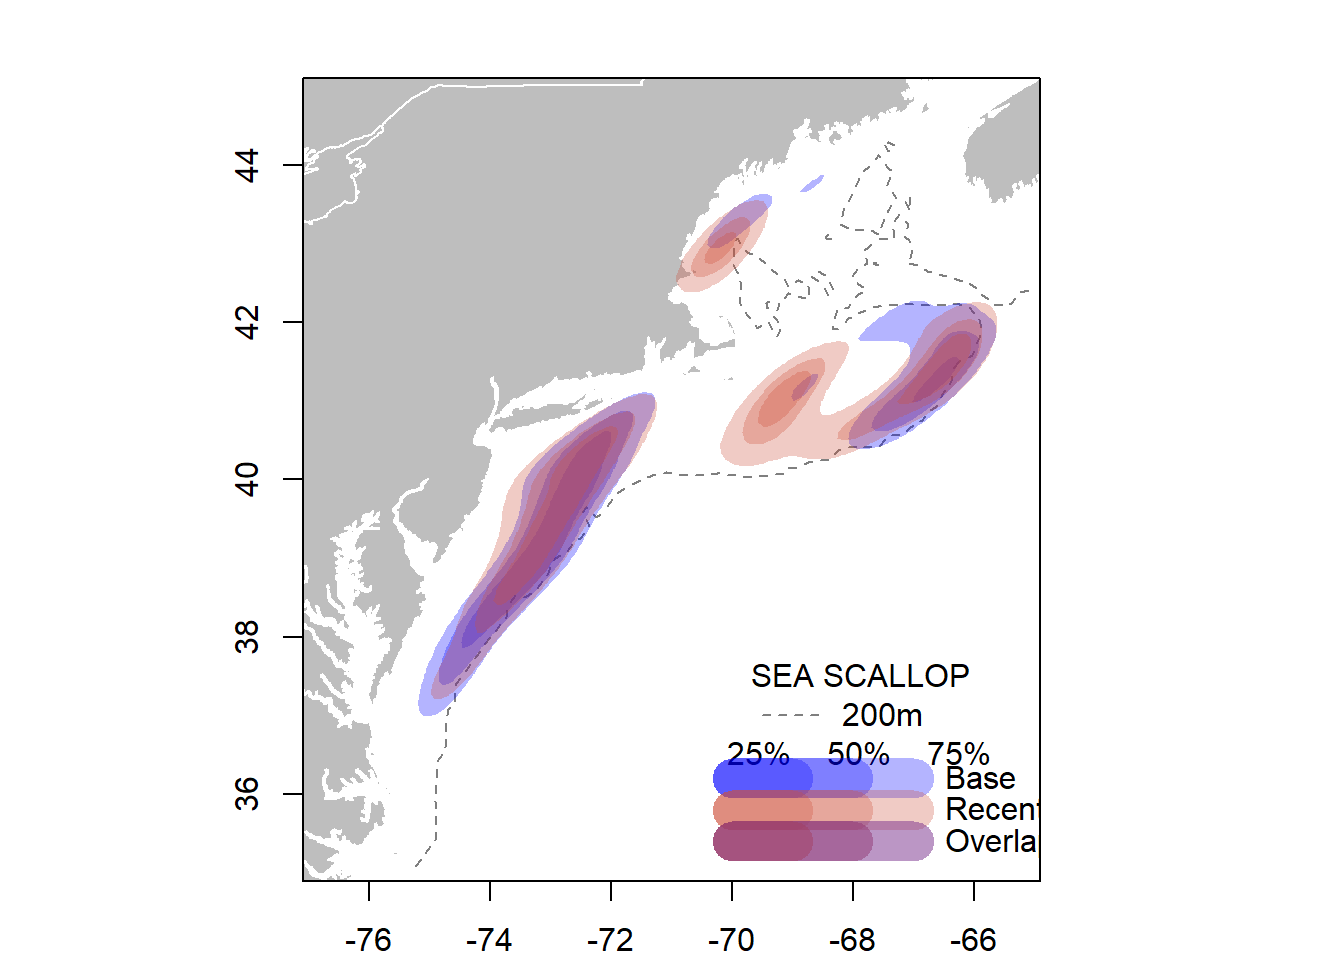
\includegraphics{C:/Users/kimberly.bastille/Desktop/tech-doc/imageskde-fig-1.pdf}
\caption{\label{fig:kde-fig}Current and historical sea scallop kernel
density estimates derived from spring survey data. Current estimates
derived from 2016-2018 data.}
\end{figure}

\chapter{Species Distribution
Indicators}\label{species-distribution-indicators}

\textbf{Description}: Species mean depth, along-shelf distance, and
distance to coastline

\textbf{Found in}: State of the Ecosystem - Gulf of Maine \& Georges
Bank (2017, 2018, 2019), State of the Ecosystem - Mid-Atlantic (2017,
2018, 2019)

\textbf{Indicator category}: Extensive analysis; not yet published

\textbf{Contributor(s)}: Kevin Friedland

\textbf{Data steward}: Kevin Friedland,
\href{mailto:kevin.friedland@noaa.gov}{\nolinkurl{kevin.friedland@noaa.gov}}

\textbf{Point of contact}: Kevin Friedland,
\href{mailto:kevin.friedland@noaa.gov}{\nolinkurl{kevin.friedland@noaa.gov}}

\textbf{Public availability statement}: Source data are available upon
request (read more
\href{https://inport.nmfs.noaa.gov/inport/item/22560}{here}). Derived
data may be downloaded
\href{https://comet.nefsc.noaa.gov/erddap/tabledap/SOE_habitat_soe_v1.html}{here}.

\section{Methods}\label{methods-29}

Three metrics quantifying spatial-temporal distribution shifts within
fish populations were developed by Friedland et al.
(\protect\hyperlink{ref-Friedland2018}{2018}), including mean depth,
along-shelf distance, and distance to coastline. Along-shelf distance is
a metric for quantifying the distribution of a species through time
along the axis of the US Northeast Continental Shelf, which extends
northeastward from the Outer Banks of North Carolina. Values in the
derived time series correspond to mean distance in km from the southwest
origin of the along-shelf axis at 0 km. The along-shelf axis begins at
76.53°W 34.60°N and terminates at 65.71°W 43.49°N.

Once mean distance is found, depth of occurrence and distance to
coastline can be calculated for each species' positional center.
Analyses present in the State of the Ecosystem (SOE) reports include
mean depth and along-shelf distance for Atlantic cod, sea scallop,
summer flounder, and black sea bass.

\subsection{Data sources}\label{data-sources-29}

Data for these indicators were derived from fishery-independent bottom
trawl survey data collected by the Northeast Fisheries Science Center
(NEFSC).

\subsection{Data analysis}\label{data-analysis-27}

Species distribution indicators were derived using the following R code.

\begin{Shaded}
\begin{Highlighting}[]
\KeywordTok{library}\NormalTok{(raster)}
\KeywordTok{library}\NormalTok{(ncdf4)}
\KeywordTok{library}\NormalTok{(stats)}
\KeywordTok{library}\NormalTok{(geosphere)}
\KeywordTok{library}\NormalTok{(plyr)}

\CommentTok{# set wd C:\textbackslash{}1_analyses_ne_shelf\textbackslash{}along shelf pos}
\CommentTok{#setwd(choose.dir(default=getwd()))}
\KeywordTok{setwd}\NormalTok{(}\StringTok{"C:/1_analyses_ne_shelf/along shelf pos"}\NormalTok{)}
\NormalTok{wd=}\KeywordTok{getwd}\NormalTok{()}


\CommentTok{# name of survey data file select season <<<<<<<<<<<<<<<<<<<<<<<<<<<<<<<<<<<<<<<<<}
\NormalTok{surfilename=}\StringTok{"Survdat_8_2017.Rdata"}

\CommentTok{# select season SPRING <<<<<<<<<<<<<<<<<<<<<<<<<<<<<<<<<<<<<<<<<<<<<<<<<<<<<<<<<<<}
\NormalTok{selseaon=}\StringTok{"SPRING"}
\NormalTok{outfile=}\StringTok{"dhdc_8_2017_fallASS_sprDATA.csv"}
\NormalTok{outfile=}\StringTok{"dhdc_8_2017_fallASS_sprDATA jc.csv"}
\NormalTok{outfile=}\StringTok{"dhdc_8_2017_fallASS_sprDATA joe.csv"}
\NormalTok{outfile=}\StringTok{"dhdc_8_2017_fallASS_sprDATA all.csv"}

\CommentTok{# select season FALL <<<<<<<<<<<<<<<<<<<<<<<<<<<<<<<<<<<<<<<<<<<<<<<<<<<<<<<<<<<<<}
\NormalTok{selseaon=}\StringTok{"FALL"}
\CommentTok{#outfile="dhdc_1_2017_sprASS_fallDATA.csv"}
\NormalTok{outfile=}\StringTok{"dhdc_1_2017_sprASS_fallDATA jc.csv"}
\NormalTok{outfile=}\StringTok{"dhdc_1_2017_sprASS_fallDATA joe.csv"}
\NormalTok{outfile=}\StringTok{"dhdc_1_2017_sprASS_fallDATA all.csv"}


\CommentTok{# read species list  sps.csv}
\CommentTok{#sps=read.csv(file.choose(), header = TRUE)}
\NormalTok{sps=}\KeywordTok{read.csv}\NormalTok{(}\DataTypeTok{file=}\StringTok{"sps.csv"}\NormalTok{, }\DataTypeTok{header =} \OtherTok{TRUE}\NormalTok{)}
\NormalTok{sps=}\KeywordTok{read.csv}\NormalTok{(}\DataTypeTok{file=}\StringTok{"sps 312.csv"}\NormalTok{, }\DataTypeTok{header =} \OtherTok{TRUE}\NormalTok{)}
\NormalTok{sps=}\KeywordTok{read.csv}\NormalTok{(}\DataTypeTok{file=}\StringTok{"sps_joe.csv"}\NormalTok{, }\DataTypeTok{header =} \OtherTok{TRUE}\NormalTok{)}
\NormalTok{sps=}\KeywordTok{read.csv}\NormalTok{(}\DataTypeTok{file=}\StringTok{"sps_spring.csv"}\NormalTok{, }\DataTypeTok{header =} \OtherTok{TRUE}\NormalTok{)}
\NormalTok{sps=}\KeywordTok{read.csv}\NormalTok{(}\DataTypeTok{file=}\StringTok{"sps_fall.csv"}\NormalTok{, }\DataTypeTok{header =} \OtherTok{TRUE}\NormalTok{)}
\NormalTok{numsps=}\KeywordTok{nrow}\NormalTok{(sps)}


\CommentTok{# select species to analyze <<<<<<<<<<<<<<<<<<<<<<<<<<<<<<<<<<<<<<<<<<<<<<<<}
\NormalTok{spptokeep=sps}\OperatorTok{$}\NormalTok{SVSPP}
\CommentTok{#spptokeep=c(73,74,75,76,77)}
\CommentTok{#spptokeep=c(312)  #Jonah Crab  312}


\CommentTok{# read in depth grid}
\NormalTok{gdepth=}\KeywordTok{raster}\NormalTok{(}\StringTok{"nes_bath_data.nc"}\NormalTok{, }\DataTypeTok{band=}\DecValTok{1}\NormalTok{)}

\CommentTok{# read in coordinates for along shelf diagnal  diag.csv}
\CommentTok{#diag=read.csv(file.choose(), header = TRUE)}
\NormalTok{diag=}\KeywordTok{read.csv}\NormalTok{(}\DataTypeTok{file=}\StringTok{"diag.csv"}\NormalTok{, }\DataTypeTok{header =} \OtherTok{TRUE}\NormalTok{)}

\CommentTok{# read in coordinate for coast     nes_coastline.csv}
\CommentTok{#nescoast=read.csv(file.choose(), header = TRUE)}
\NormalTok{nescoast=}\KeywordTok{read.csv}\NormalTok{(}\DataTypeTok{file=}\StringTok{"nes_coastline.csv"}\NormalTok{, }\DataTypeTok{header =} \OtherTok{TRUE}\NormalTok{)}

\CommentTok{# read in coordinate for coast     nes_coast_2.csv}
\CommentTok{#nescoast2=read.csv(file.choose(), header = TRUE)}
\NormalTok{nescoast2=}\KeywordTok{read.csv}\NormalTok{(}\DataTypeTok{file=}\StringTok{"nes_coast_2.csv"}\NormalTok{, }\DataTypeTok{header =} \OtherTok{TRUE}\NormalTok{)}

\CommentTok{# read in coordinate for coast V2     hersey_high_2.csv}
\CommentTok{#nesc2=read.csv(file.choose(), header = TRUE)}
\NormalTok{nesc2=}\KeywordTok{read.csv}\NormalTok{(}\DataTypeTok{file=}\StringTok{"hersey_high_2.csv"}\NormalTok{, }\DataTypeTok{header =} \OtherTok{TRUE}\NormalTok{)}

\CommentTok{# constants}
\NormalTok{radt=pi}\OperatorTok{/}\DecValTok{180}
\NormalTok{R <-}\StringTok{ }\DecValTok{6371} \CommentTok{# Earth mean radius [km]}




\CommentTok{# CODE TO READ IN STRATA COMPUTE AREAS, NOW JUST READ IN STRATAREAS dataframe}
\CommentTok{# readin in strata.shp and compute areas of strata}
\CommentTok{#TrawlStrata<-shapefile(file.choose())}
\CommentTok{#plot(TrawlStrata)}
\CommentTok{#AREA<-areaPolygon(TrawlStrata, r=6371000)/10^6}

\CommentTok{# for array of strata and area and make into dataframe}
\CommentTok{#stratareas=cbind(TrawlStrata@data$STRATA, AREA)}
\CommentTok{#colnames(stratareas) <- c("STRATA","AREA")}
\CommentTok{#stratareas=data.frame(stratareas)}
\CommentTok{#save(stratareas, file="stratareas.rdata")}

\CommentTok{# load stratareas}
\KeywordTok{load}\NormalTok{(}\StringTok{"stratareas.rdata"}\NormalTok{)}


\CommentTok{# get durvey datafile  Survdat.RData}
\CommentTok{#load(file.choose())}
\CommentTok{#load(file="Survdat.RData")}
\KeywordTok{load}\NormalTok{(}\DataTypeTok{file=}\NormalTok{surfilename)}

\CommentTok{# trin the data.... need to choose season}
\NormalTok{retvars <-}\StringTok{ }\KeywordTok{c}\NormalTok{(}\StringTok{"CRUISE6"}\NormalTok{,}\StringTok{"STATION"}\NormalTok{,}\StringTok{"STRATUM"}\NormalTok{,}\StringTok{"SVSPP"}\NormalTok{,}\StringTok{"YEAR"}\NormalTok{,}\StringTok{"SEASON"}\NormalTok{,}\StringTok{"LAT"}\NormalTok{,}\StringTok{"LON"}\NormalTok{,}\StringTok{"DEPTH"}\NormalTok{,}\StringTok{"ABUNDANCE"}\NormalTok{,}\StringTok{"BIOMASS"}\NormalTok{)}
\NormalTok{survdat <-}\StringTok{ }\NormalTok{survdat[retvars]         }
\NormalTok{survdat <-}\StringTok{ }\NormalTok{survdat[(survdat}\OperatorTok{$}\NormalTok{SEASON}\OperatorTok{==}\NormalTok{selseaon),]}

\CommentTok{# stata to use}
\CommentTok{# offshore strata to use}
\NormalTok{CoreOffshoreStrata<-}\KeywordTok{c}\NormalTok{(}\KeywordTok{seq}\NormalTok{(}\DecValTok{1010}\NormalTok{,}\DecValTok{1300}\NormalTok{,}\DecValTok{10}\NormalTok{),}\DecValTok{1340}\NormalTok{, }\KeywordTok{seq}\NormalTok{(}\DecValTok{1360}\NormalTok{,}\DecValTok{1400}\NormalTok{,}\DecValTok{10}\NormalTok{),}\KeywordTok{seq}\NormalTok{(}\DecValTok{1610}\NormalTok{,}\DecValTok{1760}\NormalTok{,}\DecValTok{10}\NormalTok{))}
\CommentTok{# inshore strata to use, still sampled by Bigelow}
\NormalTok{CoreInshore73to12=}\KeywordTok{c}\NormalTok{(}\DecValTok{3020}\NormalTok{, }\DecValTok{3050}\NormalTok{, }\DecValTok{3080}\NormalTok{ ,}\DecValTok{3110}\NormalTok{ ,}\DecValTok{3140}\NormalTok{ ,}\DecValTok{3170}\NormalTok{, }\DecValTok{3200}\NormalTok{, }\DecValTok{3230}\NormalTok{, }\DecValTok{3260}\NormalTok{, }\DecValTok{3290}\NormalTok{, }\DecValTok{3320}\NormalTok{, }\DecValTok{3350}\NormalTok{ ,}\DecValTok{3380}\NormalTok{, }\DecValTok{3410}\NormalTok{ ,}\DecValTok{3440}\NormalTok{)}
\CommentTok{# combine}
\NormalTok{strata_used=}\KeywordTok{c}\NormalTok{(CoreOffshoreStrata,CoreInshore73to12)}

\CommentTok{# find records to keep based on core strata}
\NormalTok{rectokeep=survdat}\OperatorTok{$}\NormalTok{STRATUM }\OperatorTok\StringTok{ }\NormalTok{strata_used}

\CommentTok{#table(rectokeep)}
\CommentTok{# add rec to keep to survdat}
\NormalTok{survdat=}\KeywordTok{cbind}\NormalTok{(survdat,rectokeep)}

\CommentTok{# delete record form non-core strata}
\NormalTok{survdat=survdat[}\OperatorTok{!}\NormalTok{survdat}\OperatorTok{$}\NormalTok{rectokeep}\OperatorTok{==}\StringTok{"FALSE"}\NormalTok{,]}

\CommentTok{# get rid of species}
\NormalTok{survdat}\OperatorTok{$}\NormalTok{rectokeep=survdat}\OperatorTok{$}\NormalTok{SVSPP }\OperatorTok\StringTok{ }\NormalTok{spptokeep}
\NormalTok{survdat=survdat[}\OperatorTok{!}\NormalTok{survdat}\OperatorTok{$}\NormalTok{rectokeep}\OperatorTok{==}\StringTok{"FALSE"}\NormalTok{,]}


\CommentTok{# find unique tow records only, since length and weight removed}
\CommentTok{# unique deletes to one record per species}
\NormalTok{survdat <-}\StringTok{ }\KeywordTok{unique}\NormalTok{(survdat)}

\CommentTok{# add field with rounded BIOMASS scaler used to adjust distributions}
\NormalTok{survdat}\OperatorTok{$}\NormalTok{LOGBIO <-}\StringTok{ }\KeywordTok{round}\NormalTok{(}\KeywordTok{log10}\NormalTok{(survdat}\OperatorTok{$}\NormalTok{BIOMASS }\OperatorTok{*}\StringTok{ }\DecValTok{10}\OperatorTok{+}\DecValTok{10}\NormalTok{))}
\CommentTok{# take a look go from 1 to 5?}
\KeywordTok{table}\NormalTok{(survdat}\OperatorTok{$}\NormalTok{LOGBIO)}

\CommentTok{# trim the data.... to prepare to find stations only}
\NormalTok{retvars <-}\StringTok{ }\KeywordTok{c}\NormalTok{(}\StringTok{"CRUISE6"}\NormalTok{,}\StringTok{"STATION"}\NormalTok{,}\StringTok{"STRATUM"}\NormalTok{,}\StringTok{"YEAR"}\NormalTok{)}
\NormalTok{survdat_stations <-}\StringTok{ }\NormalTok{survdat[retvars]        }
\CommentTok{# unique reduces to a record per tow}
\NormalTok{survdat_stations <-}\StringTok{ }\KeywordTok{unique}\NormalTok{(survdat_stations)}


\CommentTok{# make table of strata by year}
\NormalTok{numtowsstratyr=}\KeywordTok{table}\NormalTok{(survdat_stations}\OperatorTok{$}\NormalTok{STRATUM,survdat_stations}\OperatorTok{$}\NormalTok{YEAR)}

\CommentTok{# find records to keep based on core strata}
\NormalTok{rectokeep=stratareas}\OperatorTok{$}\NormalTok{STRATA }\OperatorTok\StringTok{ }\NormalTok{strata_used}

\CommentTok{# add rec to keep to survdat}
\NormalTok{stratareas=}\KeywordTok{cbind}\NormalTok{(stratareas,rectokeep)}

\CommentTok{# delete record form non-core strata}
\NormalTok{stratareas_usedonly=stratareas[}\OperatorTok{!}\NormalTok{stratareas}\OperatorTok{$}\NormalTok{rectokeep}\OperatorTok{==}\StringTok{"FALSE"}\NormalTok{,]}

\CommentTok{# creat areapertow}
\NormalTok{areapertow=numtowsstratyr}

\CommentTok{#compute area covered per tow per strata per year}
\ControlFlowTok{for}\NormalTok{(i }\ControlFlowTok{in} \DecValTok{1}\OperatorTok{:}\DecValTok{47}\NormalTok{)\{}
\NormalTok{  areapertow[,i]=stratareas_usedonly}\OperatorTok{$}\NormalTok{AREA}\OperatorTok{/}\NormalTok{numtowsstratyr[,i]}
\NormalTok{\}}

\CommentTok{# change inf to NA and round and out in DF}
\NormalTok{areapertow[][}\KeywordTok{is.infinite}\NormalTok{(areapertow[])]=}\OtherTok{NA}
\NormalTok{areapertow=}\KeywordTok{round}\NormalTok{(areapertow)}
\NormalTok{areapertow=}\KeywordTok{data.frame}\NormalTok{(areapertow)}
\KeywordTok{colnames}\NormalTok{(areapertow) <-}\StringTok{ }\KeywordTok{c}\NormalTok{(}\StringTok{"STRATA"}\NormalTok{,}\StringTok{"YEAR"}\NormalTok{,}\StringTok{"AREAWT"}\NormalTok{)}

\CommentTok{# add col to survdat for strata weight}
\NormalTok{survdat}\OperatorTok{$}\NormalTok{AREAPERTOW=}\OtherTok{NA}

\CommentTok{#fill AREAPERTOW}
\NormalTok{dimsurvdat=}\KeywordTok{dim}\NormalTok{(survdat)}
\ControlFlowTok{for}\NormalTok{ (i }\ControlFlowTok{in} \DecValTok{1}\OperatorTok{:}\NormalTok{dimsurvdat[}\DecValTok{1}\NormalTok{])\{}
\NormalTok{  survdat}\OperatorTok{$}\NormalTok{AREAPERTOW[i]=areapertow}\OperatorTok{$}\NormalTok{AREAWT[}\KeywordTok{which}\NormalTok{(survdat}\OperatorTok{$}\NormalTok{STRATUM[i]}\OperatorTok{==}\NormalTok{areapertow}\OperatorTok{$}\NormalTok{STRATA }\OperatorTok{&}\StringTok{ }\NormalTok{survdat}\OperatorTok{$}\NormalTok{YEAR[i]}\OperatorTok{==}\NormalTok{areapertow}\OperatorTok{$}\NormalTok{YEAR)]}
\NormalTok{\}}

\KeywordTok{table}\NormalTok{(}\KeywordTok{ceiling}\NormalTok{(survdat}\OperatorTok{$}\NormalTok{AREAPERTOW}\OperatorTok{/}\DecValTok{1000}\NormalTok{))}
\KeywordTok{table}\NormalTok{(survdat}\OperatorTok{$}\NormalTok{LOGBIO)}
\KeywordTok{table}\NormalTok{(}\KeywordTok{ceiling}\NormalTok{(survdat}\OperatorTok{$}\NormalTok{AREAPERTOW}\OperatorTok{/}\DecValTok{1000}\OperatorTok{*}\NormalTok{survdat}\OperatorTok{$}\NormalTok{LOGBIO}\OperatorTok{/}\DecValTok{9}\NormalTok{))}

\CommentTok{# add col to survdat for PLOTWT}
\NormalTok{survdat}\OperatorTok{$}\NormalTok{PLOTWT=}\OtherTok{NA}
\NormalTok{survdat}\OperatorTok{$}\NormalTok{PLOTWT=}\StringTok{ }\KeywordTok{ceiling}\NormalTok{(survdat}\OperatorTok{$}\NormalTok{AREAPERTOW}\OperatorTok{/}\DecValTok{1000}\OperatorTok{*}\NormalTok{survdat}\OperatorTok{$}\NormalTok{LOGBIO}\OperatorTok{/}\DecValTok{9}\NormalTok{)}

\KeywordTok{table}\NormalTok{(survdat}\OperatorTok{$}\NormalTok{PLOTWT)}

\CommentTok{# Plot stations}
\KeywordTok{plot}\NormalTok{(survdat}\OperatorTok{$}\NormalTok{LON[survdat}\OperatorTok{$}\NormalTok{YEAR}\OperatorTok{==}\DecValTok{1974}\NormalTok{],survdat}\OperatorTok{$}\NormalTok{LAT[survdat}\OperatorTok{$}\NormalTok{YEAR}\OperatorTok{==}\DecValTok{1974}\NormalTok{])}


\CommentTok{# put in shorter name}
\NormalTok{sdat=survdat}

\CommentTok{# clear some space}
\KeywordTok{remove}\NormalTok{(survdat)}

\CommentTok{# number of records to evaluate}
\NormalTok{numrecs=}\KeywordTok{nrow}\NormalTok{(sdat)}


\CommentTok{#======================================================================================}

\CommentTok{# TAKEN OUT SINCE THE SAME AS GASDIST}

\CommentTok{#blank array for ASDIST}
\CommentTok{#d = array(data = NA, dim =  nrow(diag))}

\CommentTok{# block to calculate diag distance  ASDIST}
\CommentTok{#for (j in 1:numrecs) \{}
\CommentTok{#   print(numrecs-j)}
\CommentTok{# }
\CommentTok{#  lat1=sdat$LAT[j]* radt}
\CommentTok{#  long1=sdat$LON[j]* radt}
\CommentTok{#  for (i in 1:150)\{}
\CommentTok{#    lat2=diag$LAT[i]* radt}
\CommentTok{#    long2=diag$LON[i]* radt}
\CommentTok{#    d[i] <- acos(sin(lat1)*sin(lat2) + cos(lat1)*cos(lat2) * cos(long2-long1)) * R}
\CommentTok{#  \}}
\CommentTok{#  dindex=which(d==min(d))}
\NormalTok{##  }
\CommentTok{#  lat1=34.60* radt}
\CommentTok{#  long1=-76.53* radt}
\CommentTok{#  }
\CommentTok{#  lat2=diag$LAT[dindex]* radt}
\CommentTok{#  long2=diag$LON[dindex]* radt}
\CommentTok{#  sdat$ASDIST[j] = acos(sin(lat1)*sin(lat2) + cos(lat1)*cos(lat2) * cos(long2-long1)) * R}
\CommentTok{#\}}


\CommentTok{#======================================================================================}

\CommentTok{# TAKEN OUT SINCE THE SAME AS GDTOC}

\CommentTok{#blank array for DTOC}
\CommentTok{#d = array(data = NA, dim = nrow(nescoast))}

\CommentTok{# block to calculate diag distance  DTOC}
\CommentTok{#for (j in 1:numrecs) \{}
\NormalTok{##  print(numrecs-j)}
  
\CommentTok{#  lat1=sdat$LAT[j]* radt}
\CommentTok{#  long1=sdat$LON[j]* radt}
\CommentTok{#  for (i in 1:nrow(nescoast))\{}
\CommentTok{#    lat2=nescoast$LAT[i]* radt}
\CommentTok{#    long2=nescoast$LON[i]* radt}
 \CommentTok{#   d[i] <- acos(sin(lat1)*sin(lat2) + cos(lat1)*cos(lat2) * cos(long2-long1)) * R}
\CommentTok{#  \}}
\CommentTok{#  sdat$DTOC[j] = d[which(d==min(d))]}
  
\CommentTok{#\}}



\CommentTok{#======================================================================================}
\KeywordTok{print}\NormalTok{(}\StringTok{"distance to coast using geosphere"}\NormalTok{)}

\NormalTok{####  Geosphere package to calc distance to coastline from pts (lon,lat), returns meters}
\NormalTok{dd =}\StringTok{ }\KeywordTok{array}\NormalTok{(}\DataTypeTok{data =} \OtherTok{NA}\NormalTok{, }\DataTypeTok{dim =} \KeywordTok{nrow}\NormalTok{(sdat))}
\NormalTok{pts =}\StringTok{ }\KeywordTok{data.frame}\NormalTok{(sdat}\OperatorTok{$}\NormalTok{LON, sdat}\OperatorTok{$}\NormalTok{LAT)}
\CommentTok{#line = t(rbind(nescoast$Longitude, nescoast$Latitude))}
\CommentTok{#line = t(rbind(nesc2$LON, nesc2$LAT))}
\NormalTok{line_nescoast2 =}\StringTok{ }\KeywordTok{t}\NormalTok{(}\KeywordTok{rbind}\NormalTok{(nescoast2}\OperatorTok{$}\NormalTok{LON, nescoast2}\OperatorTok{$}\NormalTok{LAT))}

\CommentTok{#dd=dist2Line(pts[,], line)}
\NormalTok{dd=}\KeywordTok{dist2Line}\NormalTok{(pts[,], line_nescoast2)}
\NormalTok{sdat}\OperatorTok{$}\NormalTok{GDTOC=dd}\OperatorTok{/}\DecValTok{1000} \CommentTok{# convert meters to KM}

\CommentTok{# }\AlertTok{TESTING}\CommentTok{ (look at sdat to compare dtc (geosphere) to DTOC (from loop))}
\CommentTok{# plot(line)}
\CommentTok{# lines(diag)}
\CommentTok{# lines(line)}
\CommentTok{# points(nescoast)}
\CommentTok{#ddtest=data.frame(dd)}
\CommentTok{#ddtest$distance=NULL}
\CommentTok{#plot(nescoast2)}
\CommentTok{#lines(nescoast2)}
\CommentTok{#ptt=105}
\CommentTok{#points(sdat$LON[ptt], sdat$LAT[ptt], col="red"); sdat$DTOC[ptt]; sdat$dtc[ptt]; points(ddtest[ptt,], col="green")}

\CommentTok{#======================================================================================}

\KeywordTok{print}\NormalTok{(}\StringTok{"diag distance using geosphere"}\NormalTok{)}
\CommentTok{# Find distance to diagonal line (diag), use coordinates of nearest point to find distance to NC outerbanks (min(diag))}
\NormalTok{dd2 =}\StringTok{ }\KeywordTok{array}\NormalTok{(}\DataTypeTok{data =} \OtherTok{NA}\NormalTok{, }\DataTypeTok{dim =} \KeywordTok{nrow}\NormalTok{(sdat))}
\NormalTok{dd2 =}\StringTok{ }\KeywordTok{dist2Line}\NormalTok{(pts[,], diag, }\DataTypeTok{distfun=}\NormalTok{distHaversine)}
\CommentTok{#Distance of closest point to data along diag line to NC coast}
\NormalTok{p1 =}\StringTok{ }\NormalTok{diag[}\DecValTok{1}\NormalTok{,] }\CommentTok{#start of line}
\NormalTok{p3 =}\StringTok{ }\NormalTok{diag[}\DecValTok{150}\NormalTok{,] }\CommentTok{#end of line}
\NormalTok{p2 =}\StringTok{ }\KeywordTok{data.frame}\NormalTok{(dd2[,}\DecValTok{2}\NormalTok{], dd2[,}\DecValTok{3}\NormalTok{])}
\NormalTok{distNC =}\StringTok{ }\KeywordTok{distCosine}\NormalTok{(p1, p2, }\DataTypeTok{r=}\DecValTok{6378137}\NormalTok{) }\OperatorTok{/}\DecValTok{1000} \CommentTok{# convert to KM (Great circle distance)}
\NormalTok{sdat}\OperatorTok{$}\NormalTok{GASDIST =}\StringTok{ }\NormalTok{distNC}


\CommentTok{#======================================================================================}


\CommentTok{# create column for missing depth data intially with depth data}
\NormalTok{sdat}\OperatorTok{$}\NormalTok{MISDEPTH=sdat}\OperatorTok{$}\NormalTok{DEPTH}

\CommentTok{# find cases with missing depth data}
\NormalTok{missingdepth=}\KeywordTok{which}\NormalTok{(}\KeywordTok{is.na}\NormalTok{(sdat}\OperatorTok{$}\NormalTok{DEPTH))}

\CommentTok{# fill only those records in misdepth with depth from grid}
\ControlFlowTok{for}\NormalTok{(k }\ControlFlowTok{in}\NormalTok{ missingdepth)\{}
\NormalTok{  sdat}\OperatorTok{$}\NormalTok{MISDEPTH[k] =}\StringTok{ }\KeywordTok{extract}\NormalTok{(gdepth,}\KeywordTok{cbind}\NormalTok{(sdat}\OperatorTok{$}\NormalTok{LON[k],sdat}\OperatorTok{$}\NormalTok{LAT[k])) }\OperatorTok{*}\StringTok{ }\OperatorTok{-}\DecValTok{1}
\NormalTok{\}}

\CommentTok{#=========================================================================================}




\CommentTok{#outline=paste("YR",",","SVSPP",",","mASDIST",",","mDTOC",",","mMISDEPTH",",","mLAT",",","mLON",",","mGASDIST",",","mGDTOC")}
\CommentTok{#write.table(outline,file=outfile,row.name=F,col.names=F,append=TRUE)}



\NormalTok{out_data=}\KeywordTok{array}\NormalTok{(}\OtherTok{NA}\NormalTok{,}\KeywordTok{c}\NormalTok{((}\KeywordTok{max}\NormalTok{(sdat}\OperatorTok{$}\NormalTok{YEAR)}\OperatorTok{-}\KeywordTok{min}\NormalTok{(sdat}\OperatorTok{$}\NormalTok{YEAR)}\OperatorTok{+}\DecValTok{1}\NormalTok{)}\OperatorTok{*}\NormalTok{numsps,}\DecValTok{7}\NormalTok{))}

\NormalTok{row_c=}\DecValTok{0}

\ControlFlowTok{for}\NormalTok{ (i }\ControlFlowTok{in} \DecValTok{1}\OperatorTok{:}\NormalTok{numsps)\{}
  \KeywordTok{print}\NormalTok{ (i)}
  \ControlFlowTok{for}\NormalTok{(j }\ControlFlowTok{in} \KeywordTok{min}\NormalTok{(sdat}\OperatorTok{$}\NormalTok{YEAR)}\OperatorTok{:}\KeywordTok{max}\NormalTok{(sdat}\OperatorTok{$}\NormalTok{YEAR))\{}
 
\NormalTok{    row_c=row_c}\OperatorTok{+}\DecValTok{1}   
\CommentTok{#sumdist=sum(sdat$ASDIST[sdat$YEAR==j & sdat$SVSPP==sps$SVSPP[i]] *sdat$PLOTWT[sdat$YEAR==j & sdat$SVSPP==sps$SVSPP[i]])}
\CommentTok{#lendist=sum(sdat$PLOTWT[sdat$YEAR==j & sdat$SVSPP==sps$SVSPP[i]])}
\CommentTok{#mASDIST =sumdist / lendist}

\CommentTok{#sumdist=sum(sdat$DTOC[sdat$YEAR==j & sdat$SVSPP==sps$SVSPP[i]] *sdat$PLOTWT[sdat$YEAR==j & sdat$SVSPP==sps$SVSPP[i]])}
\CommentTok{#lendist=sum(sdat$PLOTWT[sdat$YEAR==j & sdat$SVSPP==sps$SVSPP[i]])}
\CommentTok{#mDTOC =sumdist / lendist}

\NormalTok{sumdepth=}\KeywordTok{sum}\NormalTok{(sdat}\OperatorTok{$}\NormalTok{MISDEPTH[sdat}\OperatorTok{$}\NormalTok{YEAR}\OperatorTok{==}\NormalTok{j }\OperatorTok{&}\StringTok{ }\NormalTok{sdat}\OperatorTok{$}\NormalTok{SVSPP}\OperatorTok{==}\NormalTok{sps}\OperatorTok{$}\NormalTok{SVSPP[i]] }\OperatorTok{*}\NormalTok{sdat}\OperatorTok{$}\NormalTok{PLOTWT[sdat}\OperatorTok{$}\NormalTok{YEAR}\OperatorTok{==}\NormalTok{j }\OperatorTok{&}\StringTok{ }\NormalTok{sdat}\OperatorTok{$}\NormalTok{SVSPP}\OperatorTok{==}\NormalTok{sps}\OperatorTok{$}\NormalTok{SVSPP[i]])}
\NormalTok{lendepth=}\KeywordTok{sum}\NormalTok{(sdat}\OperatorTok{$}\NormalTok{PLOTWT[sdat}\OperatorTok{$}\NormalTok{YEAR}\OperatorTok{==}\NormalTok{j }\OperatorTok{&}\StringTok{ }\NormalTok{sdat}\OperatorTok{$}\NormalTok{SVSPP}\OperatorTok{==}\NormalTok{sps}\OperatorTok{$}\NormalTok{SVSPP[i]])}
\NormalTok{mMISDEPTH =sumdepth }\OperatorTok{/}\StringTok{ }\NormalTok{lendepth}

\NormalTok{sumdepth=}\KeywordTok{sum}\NormalTok{(sdat}\OperatorTok{$}\NormalTok{LAT[sdat}\OperatorTok{$}\NormalTok{YEAR}\OperatorTok{==}\NormalTok{j }\OperatorTok{&}\StringTok{ }\NormalTok{sdat}\OperatorTok{$}\NormalTok{SVSPP}\OperatorTok{==}\NormalTok{sps}\OperatorTok{$}\NormalTok{SVSPP[i]] }\OperatorTok{*}\NormalTok{sdat}\OperatorTok{$}\NormalTok{PLOTWT[sdat}\OperatorTok{$}\NormalTok{YEAR}\OperatorTok{==}\NormalTok{j }\OperatorTok{&}\StringTok{ }\NormalTok{sdat}\OperatorTok{$}\NormalTok{SVSPP}\OperatorTok{==}\NormalTok{sps}\OperatorTok{$}\NormalTok{SVSPP[i]])}
\NormalTok{lendepth=}\KeywordTok{sum}\NormalTok{(sdat}\OperatorTok{$}\NormalTok{PLOTWT[sdat}\OperatorTok{$}\NormalTok{YEAR}\OperatorTok{==}\NormalTok{j }\OperatorTok{&}\StringTok{ }\NormalTok{sdat}\OperatorTok{$}\NormalTok{SVSPP}\OperatorTok{==}\NormalTok{sps}\OperatorTok{$}\NormalTok{SVSPP[i]])}
\NormalTok{mLAT =sumdepth }\OperatorTok{/}\StringTok{ }\NormalTok{lendepth}

\NormalTok{sumdepth=}\KeywordTok{sum}\NormalTok{(sdat}\OperatorTok{$}\NormalTok{LON[sdat}\OperatorTok{$}\NormalTok{YEAR}\OperatorTok{==}\NormalTok{j }\OperatorTok{&}\StringTok{ }\NormalTok{sdat}\OperatorTok{$}\NormalTok{SVSPP}\OperatorTok{==}\NormalTok{sps}\OperatorTok{$}\NormalTok{SVSPP[i]] }\OperatorTok{*}\NormalTok{sdat}\OperatorTok{$}\NormalTok{PLOTWT[sdat}\OperatorTok{$}\NormalTok{YEAR}\OperatorTok{==}\NormalTok{j }\OperatorTok{&}\StringTok{ }\NormalTok{sdat}\OperatorTok{$}\NormalTok{SVSPP}\OperatorTok{==}\NormalTok{sps}\OperatorTok{$}\NormalTok{SVSPP[i]])}
\NormalTok{lendepth=}\KeywordTok{sum}\NormalTok{(sdat}\OperatorTok{$}\NormalTok{PLOTWT[sdat}\OperatorTok{$}\NormalTok{YEAR}\OperatorTok{==}\NormalTok{j }\OperatorTok{&}\StringTok{ }\NormalTok{sdat}\OperatorTok{$}\NormalTok{SVSPP}\OperatorTok{==}\NormalTok{sps}\OperatorTok{$}\NormalTok{SVSPP[i]])}
\NormalTok{mLON =sumdepth }\OperatorTok{/}\StringTok{ }\NormalTok{lendepth}


\NormalTok{sumdepth=}\KeywordTok{sum}\NormalTok{(sdat}\OperatorTok{$}\NormalTok{GASDIST[sdat}\OperatorTok{$}\NormalTok{YEAR}\OperatorTok{==}\NormalTok{j }\OperatorTok{&}\StringTok{ }\NormalTok{sdat}\OperatorTok{$}\NormalTok{SVSPP}\OperatorTok{==}\NormalTok{sps}\OperatorTok{$}\NormalTok{SVSPP[i]] }\OperatorTok{*}\NormalTok{sdat}\OperatorTok{$}\NormalTok{PLOTWT[sdat}\OperatorTok{$}\NormalTok{YEAR}\OperatorTok{==}\NormalTok{j }\OperatorTok{&}\StringTok{ }\NormalTok{sdat}\OperatorTok{$}\NormalTok{SVSPP}\OperatorTok{==}\NormalTok{sps}\OperatorTok{$}\NormalTok{SVSPP[i]])}
\NormalTok{lendepth=}\KeywordTok{sum}\NormalTok{(sdat}\OperatorTok{$}\NormalTok{PLOTWT[sdat}\OperatorTok{$}\NormalTok{YEAR}\OperatorTok{==}\NormalTok{j }\OperatorTok{&}\StringTok{ }\NormalTok{sdat}\OperatorTok{$}\NormalTok{SVSPP}\OperatorTok{==}\NormalTok{sps}\OperatorTok{$}\NormalTok{SVSPP[i]])}
\NormalTok{mGASDIST =sumdepth }\OperatorTok{/}\StringTok{ }\NormalTok{lendepth}

\NormalTok{sumdepth=}\KeywordTok{sum}\NormalTok{(sdat}\OperatorTok{$}\NormalTok{GDTOC[sdat}\OperatorTok{$}\NormalTok{YEAR}\OperatorTok{==}\NormalTok{j }\OperatorTok{&}\StringTok{ }\NormalTok{sdat}\OperatorTok{$}\NormalTok{SVSPP}\OperatorTok{==}\NormalTok{sps}\OperatorTok{$}\NormalTok{SVSPP[i]] }\OperatorTok{*}\NormalTok{sdat}\OperatorTok{$}\NormalTok{PLOTWT[sdat}\OperatorTok{$}\NormalTok{YEAR}\OperatorTok{==}\NormalTok{j }\OperatorTok{&}\StringTok{ }\NormalTok{sdat}\OperatorTok{$}\NormalTok{SVSPP}\OperatorTok{==}\NormalTok{sps}\OperatorTok{$}\NormalTok{SVSPP[i]])}
\NormalTok{lendepth=}\KeywordTok{sum}\NormalTok{(sdat}\OperatorTok{$}\NormalTok{PLOTWT[sdat}\OperatorTok{$}\NormalTok{YEAR}\OperatorTok{==}\NormalTok{j }\OperatorTok{&}\StringTok{ }\NormalTok{sdat}\OperatorTok{$}\NormalTok{SVSPP}\OperatorTok{==}\NormalTok{sps}\OperatorTok{$}\NormalTok{SVSPP[i]])}
\NormalTok{mGDTOC =sumdepth }\OperatorTok{/}\StringTok{ }\NormalTok{lendepth}


\NormalTok{out_data[row_c,}\DecValTok{1}\NormalTok{]=j}
\NormalTok{out_data[row_c,}\DecValTok{2}\NormalTok{]=sps}\OperatorTok{$}\NormalTok{SVSPP[i]}
\NormalTok{out_data[row_c,}\DecValTok{3}\NormalTok{]=mMISDEPTH}
\NormalTok{out_data[row_c,}\DecValTok{4}\NormalTok{]=mLAT}
\NormalTok{out_data[row_c,}\DecValTok{5}\NormalTok{]=mLON}
\NormalTok{out_data[row_c,}\DecValTok{6}\NormalTok{]=mGASDIST}
\NormalTok{out_data[row_c,}\DecValTok{7}\NormalTok{]=mGDTOC}



\NormalTok{  \}  }
\NormalTok{\}}


\CommentTok{#outline=paste(j,",",sps$SVSPP[i],",",mMISDEPTH,",",mLAT,",",mLON,",",mGASDIST,",",mGDTOC)}
\CommentTok{#write.table(outline,file=outfile,row.name=F,col.names=F,append=TRUE)}

\NormalTok{out_data=}\KeywordTok{data.frame}\NormalTok{(out_data)}



\KeywordTok{names}\NormalTok{(out_data)[}\KeywordTok{names}\NormalTok{(out_data)}\OperatorTok{==}\StringTok{"X1"}\NormalTok{] <-}\StringTok{ "YR"}
\KeywordTok{names}\NormalTok{(out_data)[}\KeywordTok{names}\NormalTok{(out_data)}\OperatorTok{==}\StringTok{"X2"}\NormalTok{] <-}\StringTok{ "SP"}
\KeywordTok{names}\NormalTok{(out_data)[}\KeywordTok{names}\NormalTok{(out_data)}\OperatorTok{==}\StringTok{"X3"}\NormalTok{] <-}\StringTok{ "DEPTH"}
\KeywordTok{names}\NormalTok{(out_data)[}\KeywordTok{names}\NormalTok{(out_data)}\OperatorTok{==}\StringTok{"X4"}\NormalTok{] <-}\StringTok{ "LAT"}
\KeywordTok{names}\NormalTok{(out_data)[}\KeywordTok{names}\NormalTok{(out_data)}\OperatorTok{==}\StringTok{"X5"}\NormalTok{] <-}\StringTok{ "LON"}
\KeywordTok{names}\NormalTok{(out_data)[}\KeywordTok{names}\NormalTok{(out_data)}\OperatorTok{==}\StringTok{"X6"}\NormalTok{] <-}\StringTok{ "ASDIST"}
\KeywordTok{names}\NormalTok{(out_data)[}\KeywordTok{names}\NormalTok{(out_data)}\OperatorTok{==}\StringTok{"X7"}\NormalTok{] <-}\StringTok{ "DTEOC"}


\KeywordTok{write.csv}\NormalTok{(out_data,}\DataTypeTok{file=}\NormalTok{outfile )}
\end{Highlighting}
\end{Shaded}

\subsection{Data processing}\label{data-processing-18}

Distribution indicators were further formatted for inclusion in the
ecodata R package using the following R code.

\begin{Shaded}
\begin{Highlighting}[]
\CommentTok{#Aggregate species distribution metrics for the Northeast Shelf}

\KeywordTok{library}\NormalTok{(dplyr)}
\KeywordTok{library}\NormalTok{(tidyr)}

\NormalTok{raw.dir <-}\StringTok{ }\NormalTok{here}\OperatorTok{::}\KeywordTok{here}\NormalTok{(}\StringTok{"data-raw"}\NormalTok{)}

\NormalTok{get_species_dist <-}\StringTok{ }\ControlFlowTok{function}\NormalTok{(}\DataTypeTok{save_clean =}\NormalTok{ F)\{}

\NormalTok{  species_dist <-}\StringTok{ }\KeywordTok{read.csv}\NormalTok{(}\KeywordTok{file.path}\NormalTok{(raw.dir, }\StringTok{"sp dist.csv"}\NormalTok{))  }\OperatorTok\StringTok{ }
\StringTok{    }\NormalTok{dplyr}\OperatorTok{::}\KeywordTok{rename}\NormalTok{(}\DataTypeTok{depth =}\NormalTok{ DEPTH,}
                  \DataTypeTok{Latitude =}\NormalTok{ LAT,}
                  \DataTypeTok{Longitude =}\NormalTok{ LON,}
                  \StringTok{`}\DataTypeTok{along-shelf distance}\StringTok{`}\NormalTok{ =}\StringTok{ }\NormalTok{ASD,}
                  \StringTok{`}\DataTypeTok{distance to coast}\StringTok{`}\NormalTok{ =}\StringTok{ }\NormalTok{DTC,}
                  \DataTypeTok{Time =}\NormalTok{ Year) }\OperatorTok\StringTok{ }
\StringTok{    }\KeywordTok{gather}\NormalTok{(.,Var,Value,}\OperatorTok{-}\NormalTok{Time) }\OperatorTok\StringTok{ }
\StringTok{    }\KeywordTok{mutate}\NormalTok{(}\DataTypeTok{EPU =} \StringTok{"All"}\NormalTok{,}
           \DataTypeTok{Units =} \KeywordTok{ifelse}\NormalTok{(}\KeywordTok{str_detect}\NormalTok{(Var,}\StringTok{"distance"}\NormalTok{),}\StringTok{"km"}\NormalTok{,}
                          \KeywordTok{ifelse}\NormalTok{(}\KeywordTok{str_detect}\NormalTok{(Var,}\StringTok{"Latitude"}\NormalTok{),}
                                     \StringTok{"degreesN"}\NormalTok{,}\KeywordTok{ifelse}\NormalTok{(}\KeywordTok{str_detect}\NormalTok{(Var,}\StringTok{"Longitude"}\NormalTok{),}
                                                      \StringTok{"degreesW"}\NormalTok{,}\KeywordTok{ifelse}\NormalTok{(}\KeywordTok{str_detect}\NormalTok{(Var, }\StringTok{"depth"}\NormalTok{),}
                                                                        \StringTok{"m"}\NormalTok{,}\OtherTok{NA}\NormalTok{)))))}
  \ControlFlowTok{if}\NormalTok{ (save_clean)\{}
\NormalTok{    usethis}\OperatorTok{::}\KeywordTok{use_data}\NormalTok{(species_dist, }\DataTypeTok{overwrite =}\NormalTok{ T)}
\NormalTok{  \} }\ControlFlowTok{else}\NormalTok{ \{}
    \KeywordTok{return}\NormalTok{(species_dist)}
\NormalTok{  \}}
\NormalTok{\}}
\end{Highlighting}
\end{Shaded}

\subsection{Plotting}\label{plotting-21}

\begin{Shaded}
\begin{Highlighting}[]
\CommentTok{# Relative working directories}
\NormalTok{data.dir  <-}\StringTok{ }\NormalTok{here}\OperatorTok{::}\KeywordTok{here}\NormalTok{(}\StringTok{'data'}\NormalTok{)}
\NormalTok{r.dir <-}\StringTok{ }\NormalTok{here}\OperatorTok{::}\KeywordTok{here}\NormalTok{(}\StringTok{'R'}\NormalTok{)}

\CommentTok{# Load data}
\KeywordTok{load}\NormalTok{(}\KeywordTok{file.path}\NormalTok{(data.dir,}\StringTok{"SOE_data_erddap.Rdata"}\NormalTok{))}

\CommentTok{# Source plotting functions}
\KeywordTok{source}\NormalTok{(}\KeywordTok{file.path}\NormalTok{(r.dir,}\StringTok{"BasePlot_source.R"}\NormalTok{))}


\NormalTok{opar <-}\StringTok{ }\KeywordTok{par}\NormalTok{(}\DataTypeTok{mfrow =} \KeywordTok{c}\NormalTok{(}\DecValTok{2}\NormalTok{, }\DecValTok{1}\NormalTok{), }\DataTypeTok{mar =} \KeywordTok{c}\NormalTok{(}\DecValTok{0}\NormalTok{, }\DecValTok{0}\NormalTok{, }\DecValTok{0}\NormalTok{, }\DecValTok{0}\NormalTok{), }\DataTypeTok{oma =} \KeywordTok{c}\NormalTok{(}\FloatTok{3.5}\NormalTok{, }\DecValTok{5}\NormalTok{, }\DecValTok{2}\NormalTok{, }\DecValTok{4}\NormalTok{))}

\KeywordTok{soe.plot}\NormalTok{(SOE.data, }\StringTok{"Time"}\NormalTok{, }\StringTok{"black sea bass spring mean along-shelf dist"}\NormalTok{, }
         \DataTypeTok{stacked =} \StringTok{"A"}\NormalTok{, }\DataTypeTok{rel.y.num =} \FloatTok{1.1}\NormalTok{, }\DataTypeTok{suppressAxis =}\NormalTok{ T, }
         \DataTypeTok{line.forward =}\NormalTok{ T, }\DataTypeTok{tol =} \FloatTok{0.15}\NormalTok{, }\DataTypeTok{x.start =} \DecValTok{1963}\NormalTok{, }\DataTypeTok{end.start =} \DecValTok{2007}\NormalTok{,}
         \DataTypeTok{cex.stacked =} \FloatTok{1.5}\NormalTok{)}
\KeywordTok{soe.plot}\NormalTok{(SOE.data, }\StringTok{"Time"}\NormalTok{, }\StringTok{"black sea bass fall mean along-shelf dist"}\NormalTok{, }
         \DataTypeTok{stacked =} \StringTok{"B"}\NormalTok{, }\DataTypeTok{rel.y.num =} \FloatTok{1.1}\NormalTok{, }\DataTypeTok{tol =} \FloatTok{0.15}\NormalTok{, }\DataTypeTok{end.start =} \DecValTok{2007}\NormalTok{,}
         \DataTypeTok{cex.stacked =} \FloatTok{1.5}\NormalTok{)}
\KeywordTok{soe.stacked.axis}\NormalTok{(}\StringTok{"Year"}\NormalTok{, }\StringTok{"Mean along-shelf distance, km"}\NormalTok{, }\DataTypeTok{y.line =} \FloatTok{3.0}\NormalTok{)}
\end{Highlighting}
\end{Shaded}

\begin{figure}
\centering
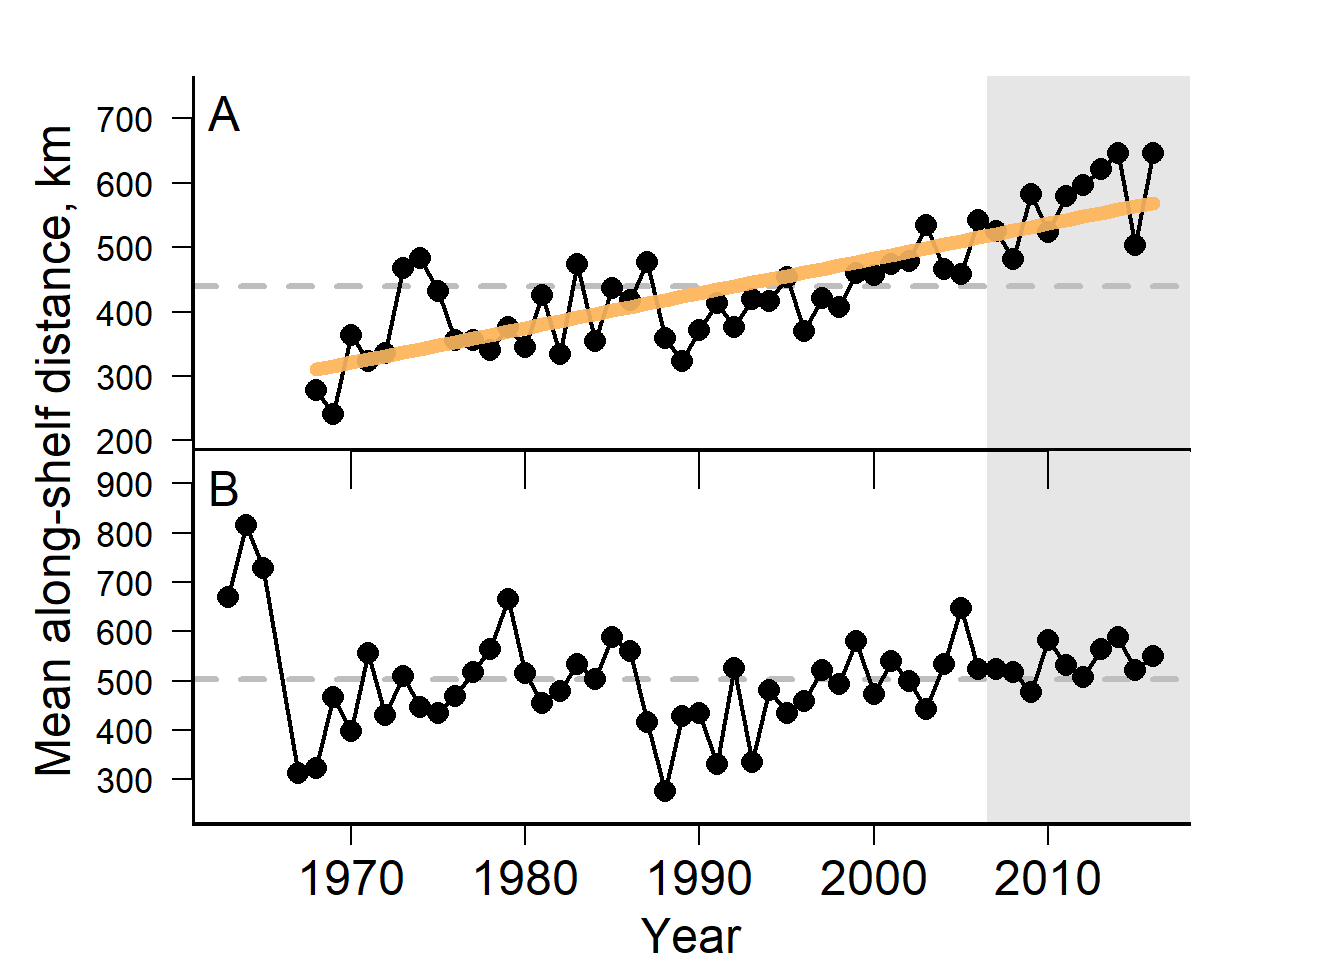
\includegraphics{C:/Users/kimberly.bastille/Desktop/tech-doc/imagesasd-bsb-1.pdf}
\caption{\label{fig:asd-bsb}Black sea bass along-shelf distance trends in
spring (A) and fall (B).}
\end{figure}

\begin{Shaded}
\begin{Highlighting}[]
\NormalTok{opar <-}\StringTok{ }\KeywordTok{par}\NormalTok{(}\DataTypeTok{mfrow =} \KeywordTok{c}\NormalTok{(}\DecValTok{2}\NormalTok{, }\DecValTok{1}\NormalTok{), }\DataTypeTok{mar =} \KeywordTok{c}\NormalTok{(}\DecValTok{0}\NormalTok{, }\DecValTok{0}\NormalTok{, }\DecValTok{0}\NormalTok{, }\DecValTok{0}\NormalTok{), }\DataTypeTok{oma =} \KeywordTok{c}\NormalTok{(}\FloatTok{3.5}\NormalTok{, }\DecValTok{5}\NormalTok{, }\DecValTok{2}\NormalTok{, }\DecValTok{4}\NormalTok{))}

\KeywordTok{soe.plot}\NormalTok{(SOE.data, }\StringTok{"Time"}\NormalTok{, }\StringTok{"black sea bass spring mean depth"}\NormalTok{, }
         \DataTypeTok{stacked =} \StringTok{"A"}\NormalTok{, }\DataTypeTok{rel.y.num =} \FloatTok{1.1}\NormalTok{, }\DataTypeTok{suppressAxis =}\NormalTok{ T, }
          \DataTypeTok{tol =} \FloatTok{0.15}\NormalTok{, }\DataTypeTok{x.start =} \DecValTok{1963}\NormalTok{, }\DataTypeTok{end.start =} \DecValTok{2007}\NormalTok{,}
         \DataTypeTok{cex.stacked =} \FloatTok{1.5}\NormalTok{)}
\KeywordTok{soe.plot}\NormalTok{(SOE.data, }\StringTok{"Time"}\NormalTok{, }\StringTok{"black sea bass fall mean depth"}\NormalTok{, }
         \DataTypeTok{stacked =} \StringTok{"B"}\NormalTok{, }\DataTypeTok{rel.y.num =} \FloatTok{1.1}\NormalTok{, }\DataTypeTok{tol =} \FloatTok{0.15}\NormalTok{, }\DataTypeTok{end.start =} \DecValTok{2007}\NormalTok{,}\DataTypeTok{line.forward =}\NormalTok{ T,}
         \DataTypeTok{cex.stacked =} \FloatTok{1.5}\NormalTok{)}
\KeywordTok{soe.stacked.axis}\NormalTok{(}\StringTok{"Year"}\NormalTok{, }\StringTok{"Mean depth, m"}\NormalTok{, }\DataTypeTok{y.line =} \FloatTok{3.0}\NormalTok{)}
\end{Highlighting}
\end{Shaded}

\begin{figure}
\centering
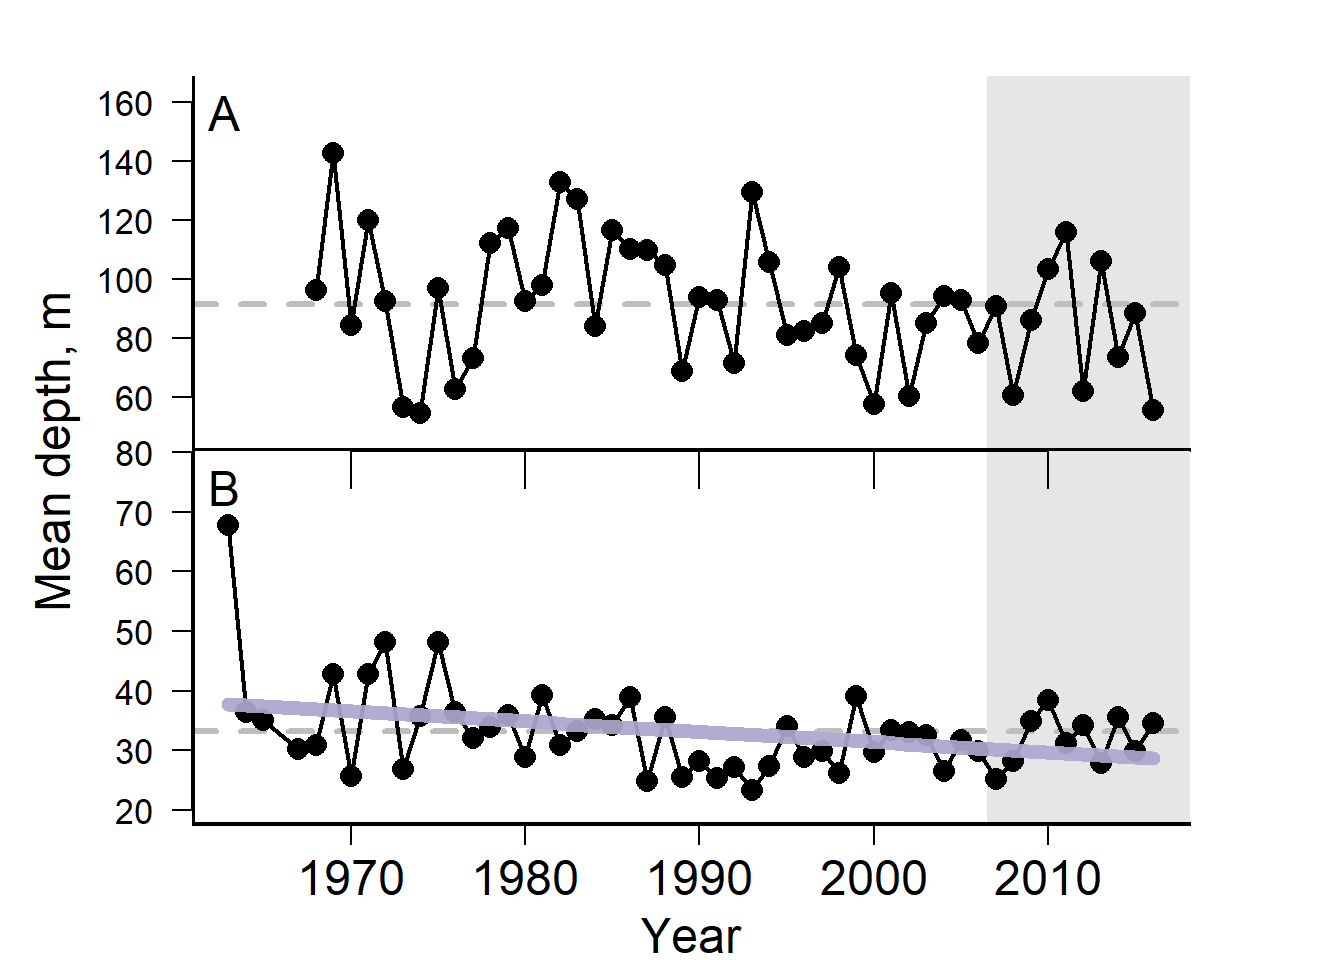
\includegraphics{C:/Users/kimberly.bastille/Desktop/tech-doc/imagesmean-depth-bsb-1.pdf}
\caption{\label{fig:mean-depth-bsb}Mean depth of black sea bass in spring
(A) and fall (B) on the Northeast Continental Shelf.}
\end{figure}

\hypertarget{survdat}{\chapter{Survey Data}\label{survdat}}

\textbf{Description}: Survdat (Survey database)

\textbf{Found in}: State of the Ecosystem - Gulf of Maine \& Georges
Bank (2017, 2018, 2019), State of the Ecosystem - Mid-Atlantic (2017,
2018, 2019)

\textbf{Indicator category}: Database pull

\textbf{Contributor(s)}: Sean Lucey

\textbf{Data steward}: Sean Lucey
\href{mailto:sean.lucey@noaa.gov}{\nolinkurl{sean.lucey@noaa.gov}}

\textbf{Point of contact}: Sean Lucey
\href{mailto:sean.lucey@noaa.gov}{\nolinkurl{sean.lucey@noaa.gov}}

\textbf{Public availability statement}: Source data are available to
qualified researchers upon request (see ``Access Information''
\href{https://inport.nmfs.noaa.gov/inport/item/22560}{here}). Derived
data used in SOE reports are available
\href{https://comet.nefsc.noaa.gov/erddap/tabledap/group_landings_soe_v1.html}{here}.

\section{Methods}\label{methods-30}

The Northeast Fisheries Science Center (NEFSC) has been conducting
standardized bottom trawl surveys in the fall since 1963 and spring
since 1968. The surveys follow a stratified random design. Fish species
and several invertebrate species are enumerated on a tow by tow basis
(Azarovitz \protect\hyperlink{ref-Azarovitz1981}{1981}).\\
The data are housed in the NEFSC's survey database (SVDBS) maintained by
the Ecosystem Survey Branch.

Direct pulls from the database are not advisable as there have been
several gear modifications and vessel changes over the course of the
time series (Miller et al. \protect\hyperlink{ref-Miller_2010}{2010}).
Survdat was developed as a database query that applies the appropriate
calibration factors for a seamless time series since the 1960s. As such,
it is the base for many of the other analyses conducted for the State of
the Ecosystem report that involve fisheries independent data.

The Survdat script can be broken down into two sections. The first pulls
the raw data from SVDBS. While the script is able to pull data from more
than just the spring and fall bottom trawl surveys, for the purposes of
the State of the Ecosystem reports only the spring and fall data are
used. Survdat identifies those research cruises associated with the
seasonal bottom trawl surveys and pulls the station and biological data.
Station data includes tow identification (cruise, station, and stratum),
tow location and date, as well as several environmental variables
(depth, surface/bottom salinity, and surface/bottom temperature).
Stations are filtered for representativness using a station, haul, gear
(SHG) code for tows prior to 2009 and a tow, operations, gear, and
aquisition (TOGA) code from 2009 onward. The codes that correspond to a
representative tow (SHG \textless{}= 136 or TOGA \textless{}= 1324) are
the same used by assessment biologists at the NEFSC. Biological data
includes the total biomass and abundance by species, as well as lengths
and number at length.

The second section of the Survdat script applies the calibration
factors. There are four calibrartion factors applied (Table
\ref{tab:calibration}). Calibration factors are pulled directly from
SVDBS. Vessel conversions were made from either the NOAA Ship
\emph{Delaware II} or NOAA Ship \emph{Henry Bigelow} to the NOAA Ship
\emph{Albatross IV} which was the primary vessel for most of the time
series. The Albatross was decommisioned in 2009 and the Bigelow is now
the primary vessel for the bottom trawl survey.

\begin{table}

\caption{\label{tab:unnamed-chunk-67}Calibration factors for NEFSC trawl survey data}
\centering
\begin{tabular}[t]{lll}
\toprule
Name & Code & Applied\\
\midrule
Door Conversion & DCF & <1985\\
Net Conversion & GCF & 1973 - 1981 (Spring)\\
Vessel Conversion I & VCF & Delaware II records\\
Vessel Conversion II & BCF & Henry Bigelow records\\
\bottomrule
\end{tabular}
\end{table}

The output from Survdat is an RData file that contains all the station
and biological data, corrected as noted above, from the NEFSC Spring
Bottom Trawl Survey and NEFSC Fall Bottom Trawl Survey. The RData file
is a data.table, a powerful wrapper for the base data.frame
(\url{https://cran.r-project.org/web/packages/data.table/data.table.pdf}).
There are also a series of tools that have been developed in order to
utilize the Survdat data set (\url{https://github.com/slucey/RSurvey}).

\subsection{Data sources}\label{data-sources-30}

Survdat is a database query of the NEFSC survey database (SVDBS).These
data are available to qualified researchers upon request. More
information on the data request process is available under the ``Access
Information'' field
\href{https://inport.nmfs.noaa.gov/inport/item/22560}{here}.

\subsection{Data extraction}\label{data-extraction-23}

Extraction methods are described above. The following is the R code used
in the data extraction process.

\begin{Shaded}
\begin{Highlighting}[]
\CommentTok{#Survdat.r}
\CommentTok{#This script will generate data from the NEFSC bottom trawl surveys}
\CommentTok{#SML}

\CommentTok{#-------------------------------------------------------------------------------}
\CommentTok{#User parameters}
\ControlFlowTok{if}\NormalTok{(}\KeywordTok{Sys.info}\NormalTok{()[}\StringTok{'sysname'}\NormalTok{]}\OperatorTok{==}\StringTok{"Windows"}\NormalTok{)\{}
\NormalTok{  data.dir <-}\StringTok{ "L:}\CharTok{\textbackslash{}\textbackslash{}}\StringTok{Rworkspace}\CharTok{\textbackslash{}\textbackslash{}}\StringTok{RSurvey"}
\NormalTok{  out.dir  <-}\StringTok{ "L:}\CharTok{\textbackslash{}\textbackslash{}}\StringTok{EcoAP}\CharTok{\textbackslash{}\textbackslash{}}\StringTok{Data}\CharTok{\textbackslash{}\textbackslash{}}\StringTok{survey"}
  \KeywordTok{memory.limit}\NormalTok{(}\DecValTok{4000}\NormalTok{)}
\NormalTok{\}}
\ControlFlowTok{if}\NormalTok{(}\KeywordTok{Sys.info}\NormalTok{()[}\StringTok{'sysname'}\NormalTok{]}\OperatorTok{==}\StringTok{"Linux"}\NormalTok{)\{}
\NormalTok{  data.dir <-}\StringTok{ "/home/slucey/slucey/Rworkspace/RSurvey"}
\NormalTok{  out.dir  <-}\StringTok{ "/home/slucey/slucey/EcoAP/Data/survey"}
\NormalTok{  uid      <-}\StringTok{ 'slucey'}
  \KeywordTok{cat}\NormalTok{(}\StringTok{"Oracle Password: "}\NormalTok{)}
\NormalTok{  pwd <-}\StringTok{ }\KeywordTok{scan}\NormalTok{(}\KeywordTok{stdin}\NormalTok{(), }\KeywordTok{character}\NormalTok{(), }\DataTypeTok{n =} \DecValTok{1}\NormalTok{)}
\NormalTok{\}}

\NormalTok{shg.check  <-}\StringTok{ 'y'} \CommentTok{# y = use only SHG <=136 or TOGA <= 1324 (>2008)}
\NormalTok{raw.check  <-}\StringTok{ 'n'} \CommentTok{# y = save data without conversions (survdat.raw), will still }
                  \CommentTok{#     save data with conversions (survdat)}
\NormalTok{all.season <-}\StringTok{ 'n'} \CommentTok{# y = save data with purpose code 10 not just spring/fall }
                  \CommentTok{#     (survdat.allseason), will not save survdat regular}
\NormalTok{use.SAD    <-}\StringTok{ 'y'} \CommentTok{# y = grab data from Survey Analysis Database (SAD) for }
                  \CommentTok{#     assessed species}
\CommentTok{#-------------------------------------------------------------------------------}
\CommentTok{#Required packages}
\KeywordTok{library}\NormalTok{(RODBC); }\KeywordTok{library}\NormalTok{(data.table)}

\CommentTok{#-------------------------------------------------------------------------------}
\CommentTok{#Created functions}
  \CommentTok{#Convert output to text for RODBC query}
\NormalTok{sqltext <-}\StringTok{ }\ControlFlowTok{function}\NormalTok{(x)\{}
\NormalTok{  out <-}\StringTok{ }\NormalTok{x[}\DecValTok{1}\NormalTok{]}
  \ControlFlowTok{if}\NormalTok{(}\KeywordTok{length}\NormalTok{(x) }\OperatorTok{>}\StringTok{ }\DecValTok{1}\NormalTok{)\{}
    \ControlFlowTok{for}\NormalTok{(i }\ControlFlowTok{in} \DecValTok{2}\OperatorTok{:}\KeywordTok{length}\NormalTok{(x))\{}
\NormalTok{      out <-}\StringTok{ }\KeywordTok{paste}\NormalTok{(out, x[i], }\DataTypeTok{sep =} \StringTok{"','"}\NormalTok{)}
\NormalTok{    \}}
\NormalTok{  \}}
\NormalTok{  out <-}\StringTok{ }\KeywordTok{paste}\NormalTok{(}\StringTok{"'"}\NormalTok{, out, }\StringTok{"'"}\NormalTok{, }\DataTypeTok{sep =} \StringTok{''}\NormalTok{)}
  \KeywordTok{return}\NormalTok{(out)}
\NormalTok{\}}

\CommentTok{#-------------------------------------------------------------------------------}
\CommentTok{#Begin script}
\ControlFlowTok{if}\NormalTok{(}\KeywordTok{Sys.info}\NormalTok{()[}\StringTok{'sysname'}\NormalTok{]}\OperatorTok{==}\StringTok{"Windows"}\NormalTok{)\{}
\NormalTok{  channel <-}\StringTok{ }\KeywordTok{odbcDriverConnect}\NormalTok{()}
\NormalTok{\} }\ControlFlowTok{else}\NormalTok{ \{}
\NormalTok{  channel <-}\StringTok{ }\KeywordTok{odbcConnect}\NormalTok{(}\StringTok{'sole'}\NormalTok{, uid, pwd)}
\NormalTok{\}}

\CommentTok{#Generate cruise list}
\ControlFlowTok{if}\NormalTok{(all.season }\OperatorTok{==}\StringTok{ 'n'}\NormalTok{)\{}
\NormalTok{  cruise.qry <-}\StringTok{ "select unique year, cruise6, svvessel, season}
\StringTok{    from mstr_cruise}
\StringTok{    where purpose_code = 10}
\StringTok{    and year >= 1963}
\StringTok{    and (season = 'FALL'}
\StringTok{      or season = 'SPRING')}
\StringTok{    order by year, cruise6"}
\NormalTok{  \}}

\ControlFlowTok{if}\NormalTok{(all.season }\OperatorTok{==}\StringTok{ 'y'}\NormalTok{)\{}
\NormalTok{  cruise.qry <-}\StringTok{ "select unique year, cruise6, svvessel, season}
\StringTok{    from mstr_cruise}
\StringTok{    where purpose_code = 10}
\StringTok{    and year >= 1963}
\StringTok{    order by year, cruise6"}
\NormalTok{  \}}
    
\NormalTok{cruise <-}\StringTok{ }\KeywordTok{as.data.table}\NormalTok{(}\KeywordTok{sqlQuery}\NormalTok{(channel, cruise.qry))}
\NormalTok{cruise <-}\StringTok{ }\KeywordTok{na.omit}\NormalTok{(cruise)}
\KeywordTok{setkey}\NormalTok{(cruise, CRUISE6, SVVESSEL)}

\CommentTok{#Use cruise codes to select other data}
\NormalTok{cruise6 <-}\StringTok{ }\KeywordTok{sqltext}\NormalTok{(cruise}\OperatorTok{$}\NormalTok{CRUISE6)}

\CommentTok{#Station data}
\ControlFlowTok{if}\NormalTok{(shg.check }\OperatorTok{==}\StringTok{ 'y'}\NormalTok{)\{}
\NormalTok{  preHB.station.qry <-}\StringTok{ }\KeywordTok{paste}\NormalTok{(}\StringTok{"select unique cruise6, svvessel, station, stratum,}
\StringTok{                             tow, decdeg_beglat as lat, decdeg_beglon as lon, }
\StringTok{                             begin_est_towdate as est_towdate, avgdepth as depth, }
\StringTok{                             surftemp, surfsalin, bottemp, botsalin}
\StringTok{                             from Union_fscs_svsta}
\StringTok{                             where cruise6 in ("}\NormalTok{, cruise6, }\StringTok{")}
\StringTok{                             and SHG <= 136}
\StringTok{                             and cruise6 <= 200900}
\StringTok{                             order by cruise6, station"}\NormalTok{, }\DataTypeTok{sep=}\StringTok{''}\NormalTok{)}
  
\NormalTok{  HB.station.qry <-}\StringTok{ }\KeywordTok{paste}\NormalTok{(}\StringTok{"select unique cruise6, svvessel, station, stratum,}
\StringTok{                          tow, decdeg_beglat as lat, decdeg_beglon as lon, }
\StringTok{                          begin_est_towdate as est_towdate, avgdepth as depth, }
\StringTok{                          surftemp, surfsalin, bottemp, botsalin}
\StringTok{                          from Union_fscs_svsta}
\StringTok{                          where cruise6 in ("}\NormalTok{, cruise6, }\StringTok{")}
\StringTok{                          and TOGA <= 1324}
\StringTok{                          and cruise6 > 200900}
\StringTok{                          order by cruise6, station"}\NormalTok{, }\DataTypeTok{sep=}\StringTok{''}\NormalTok{)}
  
\NormalTok{  preHB.sta <-}\StringTok{ }\KeywordTok{as.data.table}\NormalTok{(}\KeywordTok{sqlQuery}\NormalTok{(channel, preHB.station.qry))}
\NormalTok{  HB.sta    <-}\StringTok{ }\KeywordTok{as.data.table}\NormalTok{(}\KeywordTok{sqlQuery}\NormalTok{(channel, HB.station.qry))}
\NormalTok{  station   <-}\StringTok{ }\KeywordTok{rbindlist}\NormalTok{(}\KeywordTok{list}\NormalTok{(preHB.sta, HB.sta))}
\NormalTok{  \}}

\ControlFlowTok{if}\NormalTok{(shg.check }\OperatorTok{==}\StringTok{ 'n'}\NormalTok{)\{}
\NormalTok{  station.qry <-}\StringTok{ }\KeywordTok{paste}\NormalTok{(}\StringTok{"select unique cruise6, svvessel, station, stratum, tow,}
\StringTok{                       decdeg_beglat as lat, decdeg_beglon as lon, }
\StringTok{                       begin_est_towdate as est_towdate, avgdepth as depth, }
\StringTok{                       surftemp, surfsalin, bottemp, botsalin}
\StringTok{                       from UNION_FSCS_SVSTA}
\StringTok{                       where cruise6 in ("}\NormalTok{, cruise6, }\StringTok{")}
\StringTok{                       order by cruise6, station"}\NormalTok{, }\DataTypeTok{sep=}\StringTok{''}\NormalTok{)}
\NormalTok{  station <-}\StringTok{ }\KeywordTok{as.data.table}\NormalTok{(}\KeywordTok{sqlQuery}\NormalTok{(channel, station.qry))}
\NormalTok{  \}}
  
\KeywordTok{setkey}\NormalTok{(station, CRUISE6, SVVESSEL)}

\CommentTok{#merge cruise and station}
\NormalTok{survdat <-}\StringTok{ }\KeywordTok{merge}\NormalTok{(cruise, station)}


\CommentTok{#Catch data}
\NormalTok{catch.qry <-}\StringTok{ }\KeywordTok{paste}\NormalTok{(}\StringTok{"select cruise6, station, stratum, tow, svspp, catchsex, }
\StringTok{                   expcatchnum as abundance, expcatchwt as biomass}
\StringTok{                   from UNION_FSCS_SVCAT}
\StringTok{                   where cruise6 in ("}\NormalTok{, cruise6, }\StringTok{")}
\StringTok{                   and stratum not like 'YT%'}
\StringTok{                   order by cruise6, station, svspp"}\NormalTok{, }\DataTypeTok{sep=}\StringTok{''}\NormalTok{)}

\NormalTok{catch <-}\StringTok{ }\KeywordTok{as.data.table}\NormalTok{(}\KeywordTok{sqlQuery}\NormalTok{(channel, catch.qry))}
\KeywordTok{setkey}\NormalTok{(catch, CRUISE6, STATION, STRATUM, TOW)}

\CommentTok{#merge with survdat}
\KeywordTok{setkey}\NormalTok{(survdat, CRUISE6, STATION, STRATUM, TOW)}
\NormalTok{survdat <-}\StringTok{ }\KeywordTok{merge}\NormalTok{(survdat, catch, }\DataTypeTok{by =} \KeywordTok{key}\NormalTok{(survdat))}

\CommentTok{#Length data}
\NormalTok{length.qry <-}\StringTok{ }\KeywordTok{paste}\NormalTok{(}\StringTok{"select cruise6, station, stratum, tow, svspp, catchsex, }
\StringTok{                    length, expnumlen as numlen}
\StringTok{                    from UNION_FSCS_SVLEN}
\StringTok{                    where cruise6 in ("}\NormalTok{, cruise6, }\StringTok{")}
\StringTok{                    and stratum not like 'YT%'}
\StringTok{                    order by cruise6, station, svspp, length"}\NormalTok{, }\DataTypeTok{sep=}\StringTok{''}\NormalTok{)}

\NormalTok{len <-}\StringTok{ }\KeywordTok{as.data.table}\NormalTok{(}\KeywordTok{sqlQuery}\NormalTok{(channel, length.qry))}
\KeywordTok{setkey}\NormalTok{(len, CRUISE6, STATION, STRATUM, TOW, SVSPP, CATCHSEX)}

\CommentTok{#merge with survdat}
\KeywordTok{setkey}\NormalTok{(survdat, CRUISE6, STATION, STRATUM, TOW, SVSPP, CATCHSEX)}
\NormalTok{survdat <-}\StringTok{ }\KeywordTok{merge}\NormalTok{(survdat, len, }\DataTypeTok{all.x =}\NormalTok{ T)}

\ControlFlowTok{if}\NormalTok{(raw.check }\OperatorTok{==}\StringTok{ 'y'}\NormalTok{)\{}
\NormalTok{  survdat.raw <-}\StringTok{ }\NormalTok{survdat}
  \KeywordTok{save}\NormalTok{(survdat.raw, }\DataTypeTok{file =} \KeywordTok{paste}\NormalTok{(out.dir, }\StringTok{"Survdat_raw.RData"}\NormalTok{, }\DataTypeTok{sep =}\StringTok{''}\NormalTok{))}
\NormalTok{  \}}

\CommentTok{#Conversion Factors}
\CommentTok{#need to make abundance column a double instead of an integer}
\NormalTok{survdat[, ABUNDANCE }\OperatorTok{:}\ErrorTok{=}\StringTok{ }\KeywordTok{as.double}\NormalTok{(ABUNDANCE)]}

\CommentTok{#Grab all conversion factors off the network}
\NormalTok{convert.qry <-}\StringTok{ "select *}
\StringTok{  from survan_conversion_factors"}

\NormalTok{convert <-}\StringTok{ }\KeywordTok{as.data.table}\NormalTok{(}\KeywordTok{sqlQuery}\NormalTok{(channel,convert.qry))}

\CommentTok{#DCF < 1985 Door Conversion}
\NormalTok{dcf.spp <-}\StringTok{ }\NormalTok{convert[DCF_WT }\OperatorTok{>}\StringTok{ }\DecValTok{0}\NormalTok{, SVSPP]}
\ControlFlowTok{for}\NormalTok{(i }\ControlFlowTok{in} \DecValTok{1}\OperatorTok{:}\KeywordTok{length}\NormalTok{(dcf.spp))\{}
\NormalTok{  survdat[YEAR }\OperatorTok{<}\StringTok{ }\DecValTok{1985} \OperatorTok{&}\StringTok{ }\NormalTok{SVSPP }\OperatorTok{==}\StringTok{ }\NormalTok{dcf.spp[i],}
\NormalTok{      BIOMASS }\OperatorTok{:}\ErrorTok{=}\StringTok{ }\NormalTok{BIOMASS }\OperatorTok{*}\StringTok{ }\NormalTok{convert[SVSPP }\OperatorTok{==}\StringTok{ }\NormalTok{dcf.spp[i], DCF_WT]]}
\NormalTok{  \}}
\NormalTok{dcf.spp <-}\StringTok{ }\NormalTok{convert[DCF_NUM }\OperatorTok{>}\StringTok{ }\DecValTok{0}\NormalTok{, SVSPP]}
\ControlFlowTok{for}\NormalTok{(i }\ControlFlowTok{in} \DecValTok{1}\OperatorTok{:}\KeywordTok{length}\NormalTok{(dcf.spp))\{}
\NormalTok{  survdat[YEAR }\OperatorTok{<}\StringTok{ }\DecValTok{1985} \OperatorTok{&}\StringTok{ }\NormalTok{SVSPP }\OperatorTok{==}\StringTok{ }\NormalTok{dcf.spp[i],}
\NormalTok{      ABUNDANCE }\OperatorTok{:}\ErrorTok{=}\StringTok{ }\KeywordTok{round}\NormalTok{(ABUNDANCE }\OperatorTok{*}\StringTok{ }\NormalTok{convert[SVSPP }\OperatorTok{==}\StringTok{ }\NormalTok{dcf.spp[i], DCF_NUM])]}
\NormalTok{  \}}

\CommentTok{#GCF Spring 1973-1981  Net Conversion}
\NormalTok{gcf.spp <-}\StringTok{ }\NormalTok{convert[GCF_WT }\OperatorTok{>}\StringTok{ }\DecValTok{0}\NormalTok{, SVSPP]}
\ControlFlowTok{for}\NormalTok{(i }\ControlFlowTok{in} \DecValTok{1}\OperatorTok{:}\KeywordTok{length}\NormalTok{(gcf.spp))\{}
\NormalTok{  survdat[SEASON }\OperatorTok{==}\StringTok{ 'SPRING'} \OperatorTok{&}\StringTok{ }\NormalTok{YEAR }\OperatorTok{>}\StringTok{ }\DecValTok{1972} \OperatorTok{&}\StringTok{ }\NormalTok{YEAR }\OperatorTok{<}\StringTok{ }\DecValTok{1982} \OperatorTok{&}\StringTok{ }\NormalTok{SVSPP }\OperatorTok{==}\StringTok{ }\NormalTok{gcf.spp[i],}
\NormalTok{      BIOMASS }\OperatorTok{:}\ErrorTok{=}\StringTok{ }\NormalTok{BIOMASS }\OperatorTok{/}\StringTok{ }\NormalTok{convert[SVSPP }\OperatorTok{==}\StringTok{ }\NormalTok{gcf.spp[i], GCF_WT]]}
\NormalTok{  \}}
\NormalTok{gcf.spp <-}\StringTok{ }\NormalTok{convert[GCF_NUM }\OperatorTok{>}\StringTok{ }\DecValTok{0}\NormalTok{, SVSPP]}
\ControlFlowTok{for}\NormalTok{(i }\ControlFlowTok{in} \DecValTok{1}\OperatorTok{:}\KeywordTok{length}\NormalTok{(gcf.spp))\{}
\NormalTok{  survdat[SEASON }\OperatorTok{==}\StringTok{ 'SPRING'} \OperatorTok{&}\StringTok{ }\NormalTok{YEAR }\OperatorTok{>}\StringTok{ }\DecValTok{1972} \OperatorTok{&}\StringTok{ }\NormalTok{YEAR }\OperatorTok{<}\StringTok{ }\DecValTok{1982} \OperatorTok{&}\StringTok{ }\NormalTok{SVSPP }\OperatorTok{==}\StringTok{ }\NormalTok{gcf.spp[i],}
\NormalTok{      ABUNDANCE }\OperatorTok{:}\ErrorTok{=}\StringTok{ }\KeywordTok{round}\NormalTok{(ABUNDANCE }\OperatorTok{/}\StringTok{ }\NormalTok{convert[SVSPP }\OperatorTok{==}\StringTok{ }\NormalTok{gcf.spp[i], GCF_NUM])]}
\NormalTok{  \}}

\CommentTok{#VCF SVVESSEL = DE  Vessel Conversion}
\NormalTok{vcf.spp <-}\StringTok{ }\NormalTok{convert[VCF_WT }\OperatorTok{>}\StringTok{ }\DecValTok{0}\NormalTok{, SVSPP]}
\ControlFlowTok{for}\NormalTok{(i }\ControlFlowTok{in} \DecValTok{1}\OperatorTok{:}\KeywordTok{length}\NormalTok{(vcf.spp))\{}
\NormalTok{  survdat[SVVESSEL }\OperatorTok{==}\StringTok{ 'DE'} \OperatorTok{&}\StringTok{ }\NormalTok{SVSPP }\OperatorTok{==}\StringTok{ }\NormalTok{vcf.spp[i],}
\NormalTok{      BIOMASS }\OperatorTok{:}\ErrorTok{=}\StringTok{ }\NormalTok{BIOMASS }\OperatorTok{*}\StringTok{ }\NormalTok{convert[SVSPP }\OperatorTok{==}\StringTok{ }\NormalTok{vcf.spp[i], VCF_WT]]}
\NormalTok{  \}}
\NormalTok{vcf.spp <-}\StringTok{ }\NormalTok{convert[VCF_NUM }\OperatorTok{>}\StringTok{ }\DecValTok{0}\NormalTok{, SVSPP]}
\ControlFlowTok{for}\NormalTok{(i }\ControlFlowTok{in} \DecValTok{1}\OperatorTok{:}\KeywordTok{length}\NormalTok{(vcf.spp))\{}
\NormalTok{  survdat[SVVESSEL }\OperatorTok{==}\StringTok{ 'DE'} \OperatorTok{&}\StringTok{ }\NormalTok{SVSPP }\OperatorTok{==}\StringTok{ }\NormalTok{vcf.spp[i],}
\NormalTok{      ABUNDANCE }\OperatorTok{:}\ErrorTok{=}\StringTok{ }\KeywordTok{round}\NormalTok{(ABUNDANCE }\OperatorTok{*}\StringTok{ }\NormalTok{convert[SVSPP }\OperatorTok{==}\StringTok{ }\NormalTok{vcf.spp[i], VCF_NUM])]}
\NormalTok{  \}}

\CommentTok{#Bigelow >2008 Vessel Conversion - need flat files (not on network)}
\CommentTok{#Use Bigelow conversions for Pisces as well (PC)}
\NormalTok{big.fall   <-}\StringTok{ }\KeywordTok{as.data.table}\NormalTok{(}\KeywordTok{read.csv}\NormalTok{(}\KeywordTok{file.path}\NormalTok{(data.dir, }
                                               \StringTok{'bigelow_fall_calibration.csv'}\NormalTok{)))}
\NormalTok{big.spring <-}\StringTok{ }\KeywordTok{as.data.table}\NormalTok{(}\KeywordTok{read.csv}\NormalTok{(}\KeywordTok{file.path}\NormalTok{(data.dir, }
                                               \StringTok{'bigelow_spring_calibration.csv'}\NormalTok{)))}

\NormalTok{bf.spp <-}\StringTok{ }\NormalTok{big.fall[pW }\OperatorTok{!=}\StringTok{ }\DecValTok{1}\NormalTok{, svspp]}
\ControlFlowTok{for}\NormalTok{(i }\ControlFlowTok{in} \DecValTok{1}\OperatorTok{:}\KeywordTok{length}\NormalTok{(bf.spp))\{}
\NormalTok{  survdat[SVVESSEL }\OperatorTok\StringTok{ }\KeywordTok{c}\NormalTok{(}\StringTok{'HB'}\NormalTok{, }\StringTok{'PC'}\NormalTok{) }\OperatorTok{&}\StringTok{ }\NormalTok{SEASON }\OperatorTok{==}\StringTok{ 'FALL'} \OperatorTok{&}\StringTok{ }\NormalTok{SVSPP }\OperatorTok{==}\StringTok{ }\NormalTok{bf.spp[i],}
\NormalTok{      BIOMASS }\OperatorTok{:}\ErrorTok{=}\StringTok{ }\NormalTok{BIOMASS }\OperatorTok{/}\StringTok{ }\NormalTok{big.fall[svspp }\OperatorTok{==}\StringTok{ }\NormalTok{bf.spp[i], pW]]}
\NormalTok{  \}}
\NormalTok{bf.spp <-}\StringTok{ }\NormalTok{big.fall[pw }\OperatorTok{!=}\StringTok{ }\DecValTok{1}\NormalTok{, svspp]}
\ControlFlowTok{for}\NormalTok{(i }\ControlFlowTok{in} \DecValTok{1}\OperatorTok{:}\KeywordTok{length}\NormalTok{(bf.spp))\{}
\NormalTok{  survdat[SVVESSEL }\OperatorTok\StringTok{ }\KeywordTok{c}\NormalTok{(}\StringTok{'HB'}\NormalTok{, }\StringTok{'PC'}\NormalTok{) }\OperatorTok{&}\StringTok{ }\NormalTok{SEASON }\OperatorTok{==}\StringTok{ 'FALL'} \OperatorTok{&}\StringTok{ }\NormalTok{SVSPP }\OperatorTok{==}\StringTok{ }\NormalTok{bf.spp[i],}
\NormalTok{      ABUNDANCE }\OperatorTok{:}\ErrorTok{=}\StringTok{ }\KeywordTok{round}\NormalTok{(ABUNDANCE }\OperatorTok{/}\StringTok{ }\NormalTok{big.fall[svspp }\OperatorTok{==}\StringTok{ }\NormalTok{bf.spp[i], pw])]}
\NormalTok{  \}}

\NormalTok{bs.spp <-}\StringTok{ }\NormalTok{big.spring[pW }\OperatorTok{!=}\StringTok{ }\DecValTok{1}\NormalTok{, svspp]}
\ControlFlowTok{for}\NormalTok{(i }\ControlFlowTok{in} \DecValTok{1}\OperatorTok{:}\KeywordTok{length}\NormalTok{(bs.spp))\{}
\NormalTok{  survdat[SVVESSEL }\OperatorTok\StringTok{ }\KeywordTok{c}\NormalTok{(}\StringTok{'HB'}\NormalTok{, }\StringTok{'PC'}\NormalTok{) }\OperatorTok{&}\StringTok{ }\NormalTok{SEASON }\OperatorTok{==}\StringTok{ 'SPRING'} \OperatorTok{&}\StringTok{ }\NormalTok{SVSPP }\OperatorTok{==}\StringTok{ }\NormalTok{bs.spp[i],}
\NormalTok{      BIOMASS }\OperatorTok{:}\ErrorTok{=}\StringTok{ }\NormalTok{BIOMASS }\OperatorTok{/}\StringTok{ }\NormalTok{big.spring[svspp }\OperatorTok{==}\StringTok{ }\NormalTok{bs.spp[i], pW]]}
\NormalTok{  \}}
\NormalTok{bs.spp <-}\StringTok{ }\NormalTok{big.spring[pw }\OperatorTok{!=}\StringTok{ }\DecValTok{1}\NormalTok{, svspp]}
\ControlFlowTok{for}\NormalTok{(i }\ControlFlowTok{in} \DecValTok{1}\OperatorTok{:}\KeywordTok{length}\NormalTok{(bs.spp))\{}
\NormalTok{  survdat[SVVESSEL }\OperatorTok\StringTok{ }\KeywordTok{c}\NormalTok{(}\StringTok{'HB'}\NormalTok{, }\StringTok{'PC'}\NormalTok{) }\OperatorTok{&}\StringTok{ }\NormalTok{SEASON }\OperatorTok{==}\StringTok{ 'SPRING'} \OperatorTok{&}\StringTok{ }\NormalTok{SVSPP }\OperatorTok{==}\StringTok{ }\NormalTok{bs.spp[i],}
\NormalTok{      ABUNDANCE }\OperatorTok{:}\ErrorTok{=}\StringTok{ }\KeywordTok{round}\NormalTok{(ABUNDANCE }\OperatorTok{/}\StringTok{ }\NormalTok{big.spring[svspp }\OperatorTok{==}\StringTok{ }\NormalTok{bs.spp[i], pw])]}
\NormalTok{  \}}

\ControlFlowTok{if}\NormalTok{(use.SAD }\OperatorTok{==}\StringTok{ 'y'}\NormalTok{)\{}
\NormalTok{  sad.qry <-}\StringTok{ "select svspp, cruise6, stratum, tow, station, sex as catchsex,}
\StringTok{             catch_wt_B_cal, catch_no_B_cal, length, length_no_B_cal}
\StringTok{             from STOCKEFF.I_SV_MERGED_CATCH_CALIB_O"}
\NormalTok{  sad     <-}\StringTok{ }\KeywordTok{as.data.table}\NormalTok{(}\KeywordTok{sqlQuery}\NormalTok{(channel, sad.qry))}
  
  \KeywordTok{setkey}\NormalTok{(sad, CRUISE6, STRATUM, TOW, STATION, SVSPP, CATCHSEX, LENGTH)}
\NormalTok{  sad <-}\StringTok{ }\KeywordTok{unique}\NormalTok{(sad)}
\NormalTok{  survdat <-}\StringTok{ }\KeywordTok{merge}\NormalTok{(survdat, sad, }\DataTypeTok{by =} \KeywordTok{key}\NormalTok{(sad), }\DataTypeTok{all.x =}\NormalTok{ T)}
  
  \CommentTok{#Carry over SAD values to survdat columns and delete SAD columns}
\NormalTok{  survdat[}\OperatorTok{!}\KeywordTok{is.na}\NormalTok{(CATCH_WT_B_CAL),  BIOMASS   }\OperatorTok{:}\ErrorTok{=}\StringTok{ }\NormalTok{CATCH_WT_B_CAL]}
\NormalTok{  survdat[}\OperatorTok{!}\KeywordTok{is.na}\NormalTok{(CATCH_NO_B_CAL),  ABUNDANCE }\OperatorTok{:}\ErrorTok{=}\StringTok{ }\NormalTok{CATCH_NO_B_CAL]}
\NormalTok{  survdat[, NUMLEN }\OperatorTok{:}\ErrorTok{=}\StringTok{ }\KeywordTok{as.double}\NormalTok{(NUMLEN)]}
\NormalTok{  survdat[}\OperatorTok{!}\KeywordTok{is.na}\NormalTok{(LENGTH_NO_B_CAL), NUMLEN    }\OperatorTok{:}\ErrorTok{=}\StringTok{ }\NormalTok{LENGTH_NO_B_CAL]}
\NormalTok{  survdat[, }\KeywordTok{c}\NormalTok{(}\StringTok{'CATCH_WT_B_CAL'}\NormalTok{, }\StringTok{'CATCH_NO_B_CAL'}\NormalTok{, }\StringTok{'LENGTH_NO_B_CAL'}\NormalTok{) }\OperatorTok{:}\ErrorTok{=}\StringTok{ }\OtherTok{NULL}\NormalTok{]}
\NormalTok{\}}

\KeywordTok{odbcClose}\NormalTok{(channel)}

\ControlFlowTok{if}\NormalTok{(all.season }\OperatorTok{==}\StringTok{ 'n'}\NormalTok{) }\KeywordTok{save}\NormalTok{(survdat, }\DataTypeTok{file =} \KeywordTok{file.path}\NormalTok{(out.dir, }\StringTok{"Survdat.RData"}\NormalTok{))}
\ControlFlowTok{if}\NormalTok{(all.season }\OperatorTok{==}\StringTok{ 'y'}\NormalTok{) }\KeywordTok{save}\NormalTok{(survdat, }\DataTypeTok{file =} \KeywordTok{file.path}\NormalTok{(out.dir, }
                                                     \StringTok{"Survdat_allseason.RData"}\NormalTok{))}
\end{Highlighting}
\end{Shaded}

\subsection{Data analysis}\label{data-analysis-28}

The fisheries independent data contained within the Survdat is used in a
variety of products; the more complicated analyses are detailed in their
own sections. The most straightforward use of this data is for the
resource species aggregate biomass indicators. For the purposes of the
aggregate biomass indicators, fall and spring survey data are treated
separately. Additionally, all length data is dropped and species
seperated by sex at the catch level are merged back together.

For the aggregate biomass indicators, Survdat is first post stratified
into \protect\hyperlink{epu}{Ecological Production Units}. Stations are
labeled by the EPU they fall within using the \emph{over} function from
the \emph{rdgal} R package (Bivand, Keitt, and Rowlingson
\protect\hyperlink{ref-rgdal}{2018}). Next, the total number of stations
within each EPU per year is counted using unique station records.
Biomass is summed by species per year per EPU. Those sums are divided by
the appropriate station count to get the EPU mean. Finally, the mean
biomasses are summed by \protect\hyperlink{aggroups}{aggregate groups}.
These steps are encompassed in the processing code shown below, which
also includes steps taken to format the data set for inclusion in the
ecodata R package.

\begin{Shaded}
\begin{Highlighting}[]
\CommentTok{#Set up for finding survey proportions}

\CommentTok{#This script was adapted from code written by Sean Lucey at the NEFSC. Note that you }
\CommentTok{#will need the latest survdat file to get this to run successfully. }

\NormalTok{data.dir <-}\StringTok{ }\NormalTok{here}\OperatorTok{::}\KeywordTok{here}\NormalTok{(}\StringTok{"data-raw"}\NormalTok{)}
\CommentTok{#-------------------------------------------------------------------------}
\CommentTok{#Required packages}
\CommentTok{#devtools::install_github("slucey/RSurvey/Survdat")}

\KeywordTok{library}\NormalTok{(data.table); }\KeywordTok{library}\NormalTok{(rgdal); }\KeywordTok{library}\NormalTok{(Survdat)}
\KeywordTok{library}\NormalTok{(dplyr);}\KeywordTok{library}\NormalTok{(sf);}\KeywordTok{library}\NormalTok{(tidyr)}
\CommentTok{#-------------------------------------------------------------------------------}

\CommentTok{#Load raw data and get "strata" aka EPUs here}
\KeywordTok{load}\NormalTok{(}\KeywordTok{file.path}\NormalTok{(data.dir, }\StringTok{'Survdat.RData'}\NormalTok{))}

\NormalTok{strata <-}\StringTok{ }\NormalTok{ecodata}\OperatorTok{::}\NormalTok{epu_sf }\OperatorTok\StringTok{ }\KeywordTok{as}\NormalTok{(}\StringTok{"Spatial"}\NormalTok{)}

\CommentTok{#Generate area table}
\NormalTok{strat.area <-}\StringTok{ }\KeywordTok{getarea}\NormalTok{(strata, }\StringTok{'EPU'}\NormalTok{)}

\CommentTok{#Post stratify data}
\NormalTok{survdat.EPU <-}\StringTok{ }\KeywordTok{poststrat}\NormalTok{(survdat, strata, }\StringTok{'EPU'}\NormalTok{)}
\KeywordTok{setnames}\NormalTok{(survdat.EPU, }\StringTok{'newstrata'}\NormalTok{, }\StringTok{'EPU'}\NormalTok{)}

\CommentTok{#Subset by season/ strata set}
\NormalTok{fall   <-}\StringTok{ }\NormalTok{survdat.EPU[SEASON }\OperatorTok{==}\StringTok{ 'FALL'}\NormalTok{,   ]}
\NormalTok{spring <-}\StringTok{ }\NormalTok{survdat.EPU[SEASON }\OperatorTok{==}\StringTok{ 'SPRING'}\NormalTok{, ]}

\CommentTok{#Run stratification prep}
\NormalTok{fall.prep   <-}\StringTok{ }\KeywordTok{stratprep}\NormalTok{(fall,   strat.area, }\DataTypeTok{strat.col =} \StringTok{'EPU'}\NormalTok{, }\DataTypeTok{area.col =} \StringTok{'Area'}\NormalTok{)}
\NormalTok{spring.prep <-}\StringTok{ }\KeywordTok{stratprep}\NormalTok{(spring, strat.area, }\DataTypeTok{strat.col =} \StringTok{'EPU'}\NormalTok{, }\DataTypeTok{area.col =} \StringTok{'Area'}\NormalTok{)}

\CommentTok{#Calculate mean weight/tow by aggregate groups}
\CommentTok{#n tows}
\NormalTok{n.tows.fall  <-}\StringTok{ }\KeywordTok{unique}\NormalTok{(fall.prep[,   }\KeywordTok{list}\NormalTok{(YEAR, EPU, ntows)])}
\NormalTok{n.tows.spring <-}\StringTok{ }\KeywordTok{unique}\NormalTok{(spring.prep[, }\KeywordTok{list}\NormalTok{(YEAR, EPU, ntows)])}

\CommentTok{#drop length data}
\KeywordTok{setkey}\NormalTok{(fall.prep, YEAR, EPU, STATION, STRATUM, SVSPP, CATCHSEX)}
\NormalTok{fall.prep <-}\StringTok{ }\KeywordTok{unique}\NormalTok{(fall.prep, }\DataTypeTok{by =} \KeywordTok{key}\NormalTok{(fall.prep))}
\NormalTok{fall.prep[, }\KeywordTok{c}\NormalTok{(}\StringTok{'LENGTH'}\NormalTok{, }\StringTok{'NUMLEN'}\NormalTok{) }\OperatorTok{:}\ErrorTok{=}\StringTok{ }\OtherTok{NULL}\NormalTok{]}

\KeywordTok{setkey}\NormalTok{(spring.prep, YEAR, EPU, STATION, STRATUM, SVSPP, CATCHSEX)}
\NormalTok{spring.prep <-}\StringTok{ }\KeywordTok{unique}\NormalTok{(spring.prep, }\DataTypeTok{by =} \KeywordTok{key}\NormalTok{(spring.prep))}
\NormalTok{spring.prep[, }\KeywordTok{c}\NormalTok{(}\StringTok{'LENGTH'}\NormalTok{, }\StringTok{'NUMLEN'}\NormalTok{) }\OperatorTok{:}\ErrorTok{=}\StringTok{ }\OtherTok{NULL}\NormalTok{]}

\CommentTok{#Merge Sexed species}
\KeywordTok{setkey}\NormalTok{(fall.prep, YEAR, EPU, STATION, STRATUM, SVSPP)}
\NormalTok{fall.prep <-}\StringTok{ }\NormalTok{fall.prep[, }\KeywordTok{sum}\NormalTok{(BIOMASS, }\DataTypeTok{na.rm =}\NormalTok{ T), by =}\StringTok{ }\KeywordTok{key}\NormalTok{(fall.prep)]}

\KeywordTok{setkey}\NormalTok{(spring.prep, YEAR, EPU, STATION, STRATUM, SVSPP)}
\NormalTok{spring.prep <-}\StringTok{ }\NormalTok{spring.prep[, }\KeywordTok{sum}\NormalTok{(BIOMASS, }\DataTypeTok{na.rm =}\NormalTok{ T), by =}\StringTok{ }\KeywordTok{key}\NormalTok{(spring.prep)]}

\CommentTok{#Sum biomass within an EPU}
\NormalTok{fall.sum   <-}\StringTok{ }\NormalTok{fall.prep[,   }\KeywordTok{sum}\NormalTok{(V1), by =}\StringTok{ }\KeywordTok{c}\NormalTok{(}\StringTok{'YEAR'}\NormalTok{, }\StringTok{'EPU'}\NormalTok{, }\StringTok{'SVSPP'}\NormalTok{)]}
\NormalTok{spring.sum <-}\StringTok{ }\NormalTok{spring.prep[, }\KeywordTok{sum}\NormalTok{(V1), by =}\StringTok{ }\KeywordTok{c}\NormalTok{(}\StringTok{'YEAR'}\NormalTok{, }\StringTok{'EPU'}\NormalTok{, }\StringTok{'SVSPP'}\NormalTok{)]}

\CommentTok{#Merge sum with station count}
\NormalTok{fall.sum   <-}\StringTok{ }\KeywordTok{merge}\NormalTok{(fall.sum,   n.tows.fall, }\DataTypeTok{by =} \KeywordTok{c}\NormalTok{(}\StringTok{'YEAR'}\NormalTok{, }\StringTok{'EPU'}\NormalTok{))}
\NormalTok{spring.sum <-}\StringTok{ }\KeywordTok{merge}\NormalTok{(spring.sum, n.tows.spring, }\DataTypeTok{by =} \KeywordTok{c}\NormalTok{(}\StringTok{'YEAR'}\NormalTok{, }\StringTok{'EPU'}\NormalTok{))}

\CommentTok{#Calculate mean weight per tow}
\NormalTok{fall.sum[, kg.per.tow }\OperatorTok{:}\ErrorTok{=}\StringTok{ }\NormalTok{V1 }\OperatorTok{/}\StringTok{ }\NormalTok{ntows]}
\NormalTok{fall.mean <-}\StringTok{ }\NormalTok{fall.sum[, }\KeywordTok{list}\NormalTok{(YEAR, EPU, SVSPP, kg.per.tow)]}

\NormalTok{spring.sum[, kg.per.tow }\OperatorTok{:}\ErrorTok{=}\StringTok{ }\NormalTok{V1 }\OperatorTok{/}\StringTok{ }\NormalTok{ntows]}
\NormalTok{spring.mean <-}\StringTok{ }\NormalTok{spring.sum[, }\KeywordTok{list}\NormalTok{(YEAR, EPU, SVSPP, kg.per.tow)]}

\CommentTok{#get species groupings}
\NormalTok{groups <-}\StringTok{ }\NormalTok{ecodata}\OperatorTok{::}\NormalTok{species_groupings }\OperatorTok\StringTok{ }
\StringTok{  }\NormalTok{dplyr}\OperatorTok{::}\KeywordTok{select}\NormalTok{(}\DataTypeTok{group =}\NormalTok{ SOE_}\DecValTok{18}\NormalTok{, SVSPP,}
                \DataTypeTok{comname =}\NormalTok{ COMNAME) }\OperatorTok\StringTok{ }
\StringTok{  }\KeywordTok{filter}\NormalTok{(}\OperatorTok{!}\KeywordTok{is.na}\NormalTok{(SVSPP)) }\OperatorTok\StringTok{ }
\StringTok{  }\KeywordTok{as.data.table}\NormalTok{()}

\CommentTok{#Aggregate by conceptual model groupings}
\NormalTok{fall   <-}\StringTok{ }\KeywordTok{merge}\NormalTok{(fall.mean,   }\KeywordTok{unique}\NormalTok{(groups[, }\KeywordTok{list}\NormalTok{(SVSPP, group, comname)]), }
                \DataTypeTok{by =} \StringTok{'SVSPP'}\NormalTok{, }\DataTypeTok{all.x =}\NormalTok{ T)}
\NormalTok{spring <-}\StringTok{ }\KeywordTok{merge}\NormalTok{(spring.mean, }\KeywordTok{unique}\NormalTok{(groups[, }\KeywordTok{list}\NormalTok{(SVSPP, group, comname)]), }
                \DataTypeTok{by =} \StringTok{'SVSPP'}\NormalTok{, }\DataTypeTok{all.x =}\NormalTok{ T)}

\CommentTok{#Fix NA group to other}
\NormalTok{fall[  }\KeywordTok{is.na}\NormalTok{(group), group }\OperatorTok{:}\ErrorTok{=}\StringTok{ 'Other'}\NormalTok{]}
\NormalTok{spring[}\KeywordTok{is.na}\NormalTok{(group), group }\OperatorTok{:}\ErrorTok{=}\StringTok{ 'Other'}\NormalTok{]}

\CommentTok{#Before aggregating, save data with species ids}
\NormalTok{spring}\OperatorTok{$}\NormalTok{season <-}\StringTok{ "spring"}
\NormalTok{fall}\OperatorTok{$}\NormalTok{season <-}\StringTok{ "fall"}

\NormalTok{survey_biomass <-}\StringTok{ }\KeywordTok{rbind}\NormalTok{(spring, fall) }\OperatorTok\StringTok{ }
\StringTok{  }\KeywordTok{filter}\NormalTok{(}\OperatorTok{!}\KeywordTok{is.na}\NormalTok{(SVSPP))}

\NormalTok{managed <-}\StringTok{ }\NormalTok{ecodata}\OperatorTok{::}\NormalTok{species_groupings }\OperatorTok\StringTok{ }
\StringTok{  }\NormalTok{dplyr}\OperatorTok{::}\KeywordTok{select}\NormalTok{(}\DataTypeTok{comname =}\NormalTok{ COMNAME, Fed_Managed)}

\NormalTok{nefsc_survey_disaggregated <-}\StringTok{ }
\StringTok{  }\NormalTok{survey_biomass }\OperatorTok\StringTok{  }
\StringTok{  }\KeywordTok{group_by}\NormalTok{(EPU, group, season, YEAR) }\OperatorTok\StringTok{ }
\StringTok{  }\KeywordTok{mutate}\NormalTok{(}\DataTypeTok{Total =} \KeywordTok{sum}\NormalTok{(kg.per.tow)) }\OperatorTok\StringTok{ }
\StringTok{  }\KeywordTok{mutate}\NormalTok{(}\DataTypeTok{Prop =}\NormalTok{ kg.per.tow}\OperatorTok{/}\NormalTok{Total) }\OperatorTok\StringTok{ }
\StringTok{  }\KeywordTok{filter}\NormalTok{(}\OperatorTok{!}\NormalTok{group }\OperatorTok\StringTok{ }\KeywordTok{c}\NormalTok{(}\StringTok{"Apex Predator"}\NormalTok{,}\StringTok{"Other"}\NormalTok{),}
\NormalTok{         EPU }\OperatorTok{!=}\StringTok{ "SS"}\NormalTok{) }\OperatorTok\StringTok{ }
\StringTok{  }\NormalTok{dplyr}\OperatorTok{::}\KeywordTok{rename}\NormalTok{(}\DataTypeTok{Time =}\NormalTok{ YEAR) }\OperatorTok\StringTok{ }
\StringTok{  }\KeywordTok{as.data.frame}\NormalTok{() }\OperatorTok\StringTok{ }
\StringTok{  }\KeywordTok{left_join}\NormalTok{(.,managed,}\DataTypeTok{by =} \KeywordTok{c}\NormalTok{(}\StringTok{"comname"}\NormalTok{) ) }\OperatorTok\StringTok{ }
\StringTok{  }\KeywordTok{distinct}\NormalTok{() }\OperatorTok\StringTok{ }
\StringTok{  }\KeywordTok{complete}\NormalTok{(}\DataTypeTok{Time =} \KeywordTok{full_seq}\NormalTok{(}\KeywordTok{min}\NormalTok{(.}\OperatorTok{$}\NormalTok{Time)}\OperatorTok{:}\KeywordTok{max}\NormalTok{(.}\OperatorTok{$}\NormalTok{Time),}\DecValTok{1}\NormalTok{),}
           \KeywordTok{nesting}\NormalTok{(EPU, Fed_Managed,season, group, comname, SVSPP)) }\OperatorTok\StringTok{ }
\StringTok{  }\NormalTok{dplyr}\OperatorTok{::}\KeywordTok{rename}\NormalTok{(}\DataTypeTok{Management =}\NormalTok{ Fed_Managed,}
                \StringTok{`}\DataTypeTok{Feeding guild}\StringTok{`}\NormalTok{ =}\StringTok{ }\NormalTok{group, }
                \DataTypeTok{Season =}\NormalTok{ season,}
                \DataTypeTok{Proportion =}\NormalTok{ Prop)}
  
\NormalTok{usethis}\OperatorTok{::}\KeywordTok{use_data}\NormalTok{(nefsc_survey_disaggregated, }\DataTypeTok{overwrite =} \OtherTok{TRUE}\NormalTok{)}

\NormalTok{## GET AGGREGATED SURVEY DATA--------------------------------------------------------}

\NormalTok{fall.agg   <-}\StringTok{ }\NormalTok{fall[,   }\KeywordTok{sum}\NormalTok{(kg.per.tow), by =}\StringTok{ }\KeywordTok{c}\NormalTok{(}\StringTok{'YEAR'}\NormalTok{, }\StringTok{'EPU'}\NormalTok{, }\StringTok{'group'}\NormalTok{)]}
\NormalTok{spring.agg <-}\StringTok{ }\NormalTok{spring[, }\KeywordTok{sum}\NormalTok{(kg.per.tow), by =}\StringTok{ }\KeywordTok{c}\NormalTok{(}\StringTok{'YEAR'}\NormalTok{, }\StringTok{'EPU'}\NormalTok{, }\StringTok{'group'}\NormalTok{)]}

\CommentTok{# #Total}
\NormalTok{fall.agg[, Total }\OperatorTok{:}\ErrorTok{=}\StringTok{ }\KeywordTok{sum}\NormalTok{(V1), by =}\StringTok{ }\KeywordTok{c}\NormalTok{(}\StringTok{'YEAR'}\NormalTok{, }\StringTok{'EPU'}\NormalTok{, }\StringTok{'group'}\NormalTok{)]}
\NormalTok{spring.agg[, Total }\OperatorTok{:}\ErrorTok{=}\StringTok{ }\KeywordTok{sum}\NormalTok{(V1), by =}\StringTok{ }\KeywordTok{c}\NormalTok{(}\StringTok{'YEAR'}\NormalTok{, }\StringTok{'EPU'}\NormalTok{, }\StringTok{'group'}\NormalTok{)]}

\CommentTok{#Get in correct long format for SOE}
\CommentTok{#By feeding guild}
\NormalTok{fall.tot <-}\StringTok{ }\KeywordTok{copy}\NormalTok{(fall.agg)}
\NormalTok{fall.tot[, Var }\OperatorTok{:}\ErrorTok{=}\StringTok{ }\KeywordTok{paste}\NormalTok{(group, }\StringTok{'Fall Biomass Index'}\NormalTok{)]}
\KeywordTok{setnames}\NormalTok{(fall.tot, }\KeywordTok{c}\NormalTok{(}\StringTok{'YEAR'}\NormalTok{, }\StringTok{'EPU'}\NormalTok{, }\StringTok{'V1'}\NormalTok{), }\KeywordTok{c}\NormalTok{(}\StringTok{'Time'}\NormalTok{, }\StringTok{'Region'}\NormalTok{, }\StringTok{'Value'}\NormalTok{))}
\NormalTok{fall.tot[, Units  }\OperatorTok{:}\ErrorTok{=}\StringTok{ 'kg tow^-1'}\NormalTok{]}
\NormalTok{fall.tot <-}\StringTok{ }\KeywordTok{unique}\NormalTok{(fall.tot)}
\NormalTok{fall.tot <-}\StringTok{ }\KeywordTok{mutate}\NormalTok{(fall.tot, }\DataTypeTok{Season =} \StringTok{"Fall"}\NormalTok{)}

\NormalTok{spring.tot <-}\StringTok{ }\KeywordTok{copy}\NormalTok{(spring.agg)}
\NormalTok{spring.tot[, Var }\OperatorTok{:}\ErrorTok{=}\StringTok{ }\KeywordTok{paste}\NormalTok{(group, }\StringTok{'Spring Biomass Index'}\NormalTok{)]}
\KeywordTok{setnames}\NormalTok{(spring.tot, }\KeywordTok{c}\NormalTok{(}\StringTok{'YEAR'}\NormalTok{, }\StringTok{'EPU'}\NormalTok{, }\StringTok{'V1'}\NormalTok{), }\KeywordTok{c}\NormalTok{(}\StringTok{'Time'}\NormalTok{, }\StringTok{'Region'}\NormalTok{, }\StringTok{'Value'}\NormalTok{))}
\NormalTok{spring.tot[, Units  }\OperatorTok{:}\ErrorTok{=}\StringTok{ 'kg tow^-1'}\NormalTok{]}
\NormalTok{spring.tot <-}\StringTok{ }\KeywordTok{unique}\NormalTok{(spring.tot)}
\NormalTok{spring.tot <-}\StringTok{ }\KeywordTok{mutate}\NormalTok{(spring.tot, }\DataTypeTok{Season =} \StringTok{"Spring"}\NormalTok{)}

\NormalTok{agg_survey <-}\StringTok{ }\KeywordTok{rbind}\NormalTok{(spring.tot, fall.tot)}

\CommentTok{#Merge into one data set}
\NormalTok{nefsc_survey <-}\StringTok{ }\NormalTok{agg_survey }\OperatorTok\StringTok{ }
\StringTok{  }\NormalTok{dplyr}\OperatorTok{::}\KeywordTok{select}\NormalTok{(Time, }\DataTypeTok{EPU =}\NormalTok{ Region, Var, Units, Value)  }\OperatorTok\StringTok{ }
\StringTok{  }\KeywordTok{distinct}\NormalTok{() }\OperatorTok\StringTok{ }
\StringTok{  }\KeywordTok{complete}\NormalTok{(}\DataTypeTok{Time =} \KeywordTok{full_seq}\NormalTok{(}\KeywordTok{min}\NormalTok{(.}\OperatorTok{$}\NormalTok{Time)}\OperatorTok{:}\KeywordTok{max}\NormalTok{(.}\OperatorTok{$}\NormalTok{Time),}\DecValTok{1}\NormalTok{),}
           \KeywordTok{nesting}\NormalTok{(EPU,Var))}

\NormalTok{usethis}\OperatorTok{::}\KeywordTok{use_data}\NormalTok{(nefsc_survey, }\DataTypeTok{overwrite =}\NormalTok{ T)}
\end{Highlighting}
\end{Shaded}

\subsection{Plotting}\label{plotting-22}

\begin{Shaded}
\begin{Highlighting}[]
\CommentTok{# Relative working directories}
\NormalTok{data.dir  <-}\StringTok{ }\NormalTok{here}\OperatorTok{::}\KeywordTok{here}\NormalTok{(}\StringTok{'data'}\NormalTok{)}
\NormalTok{r.dir <-}\StringTok{ }\NormalTok{here}\OperatorTok{::}\KeywordTok{here}\NormalTok{(}\StringTok{'R'}\NormalTok{)}

\CommentTok{# Load data}
\KeywordTok{load}\NormalTok{(}\KeywordTok{file.path}\NormalTok{(data.dir,}\StringTok{"SOE_data_erddap.Rdata"}\NormalTok{))}

\CommentTok{# Source plotting functions}
\KeywordTok{source}\NormalTok{(}\KeywordTok{file.path}\NormalTok{(r.dir,}\StringTok{"BasePlot_source.R"}\NormalTok{))}


\NormalTok{opar <-}\StringTok{ }\KeywordTok{par}\NormalTok{(}\DataTypeTok{mfrow =} \KeywordTok{c}\NormalTok{(}\DecValTok{4}\NormalTok{, }\DecValTok{1}\NormalTok{), }\DataTypeTok{mar =} \KeywordTok{c}\NormalTok{(}\DecValTok{0}\NormalTok{, }\DecValTok{0}\NormalTok{, }\DecValTok{0}\NormalTok{, }\DecValTok{0}\NormalTok{), }\DataTypeTok{oma =} \KeywordTok{c}\NormalTok{(}\DecValTok{4}\NormalTok{, }\FloatTok{6.5}\NormalTok{, }\DecValTok{2}\NormalTok{, }\DecValTok{6}\NormalTok{))}

\KeywordTok{soe.plot}\NormalTok{(SOE.data, }\StringTok{"Time"}\NormalTok{, }\StringTok{"Piscivore Fall Biomass Index MAB"}\NormalTok{, }
         \DataTypeTok{stacked =} \StringTok{"A"}\NormalTok{, }\DataTypeTok{rel.y.num =} \FloatTok{1.1}\NormalTok{, }\DataTypeTok{end.start =} \DecValTok{2007}\NormalTok{,}\DataTypeTok{cex.stacked =} \FloatTok{1.5}\NormalTok{)}
\KeywordTok{soe.plot}\NormalTok{(SOE.data, }\StringTok{"Time"}\NormalTok{, }\StringTok{"Planktivore Fall Biomass Index MAB"}\NormalTok{, }
         \DataTypeTok{stacked =} \StringTok{"B"}\NormalTok{, }\DataTypeTok{rel.y.num =} \FloatTok{1.1}\NormalTok{, }\DataTypeTok{end.start =} \DecValTok{2007}\NormalTok{,}\DataTypeTok{cex.stacked =} \FloatTok{1.5}\NormalTok{)}
\KeywordTok{soe.plot}\NormalTok{(SOE.data, }\StringTok{"Time"}\NormalTok{, }\StringTok{"Benthivore Fall Biomass Index MAB"}\NormalTok{, }
         \DataTypeTok{stacked =} \StringTok{"C"}\NormalTok{, }\DataTypeTok{rel.y.num =} \FloatTok{1.1}\NormalTok{, }\DataTypeTok{end.start =} \DecValTok{2007}\NormalTok{,}\DataTypeTok{cex.stacked =} \FloatTok{1.5}\NormalTok{)}
\KeywordTok{soe.plot}\NormalTok{(SOE.data, }\StringTok{"Time"}\NormalTok{, }\StringTok{"Benthos Fall Biomass Index MAB"}\NormalTok{, }
         \DataTypeTok{stacked =} \StringTok{"D"}\NormalTok{, }\DataTypeTok{rel.y.num =} \FloatTok{1.1}\NormalTok{, }\DataTypeTok{end.start =} \DecValTok{2007}\NormalTok{,}\DataTypeTok{cex.stacked =} \FloatTok{1.5}\NormalTok{)}
\CommentTok{#soe.plot(SOE.data, "Time", "Total Fall Biomass MAB", stacked = "E",status  = F,}
\CommentTok{#         endshade = T, rel.y.num = 1.1, full.trend = T, scale.axis = 1)}
\KeywordTok{soe.stacked.axis}\NormalTok{(}\StringTok{"Year"}\NormalTok{, }\KeywordTok{expression}\NormalTok{(}\StringTok{"Biomass, kg tow"}\OperatorTok{^-}\DecValTok{1}\NormalTok{), }\DataTypeTok{y.line =} \FloatTok{3.0}\NormalTok{,}
                 \DataTypeTok{x.line =} \FloatTok{2.7}\NormalTok{)}

\NormalTok{opar <-}\StringTok{ }\KeywordTok{par}\NormalTok{(}\DataTypeTok{mfrow =} \KeywordTok{c}\NormalTok{(}\DecValTok{4}\NormalTok{, }\DecValTok{1}\NormalTok{), }\DataTypeTok{mar =} \KeywordTok{c}\NormalTok{(}\DecValTok{0}\NormalTok{, }\DecValTok{0}\NormalTok{, }\DecValTok{0}\NormalTok{, }\DecValTok{0}\NormalTok{), }\DataTypeTok{oma =} \KeywordTok{c}\NormalTok{(}\DecValTok{4}\NormalTok{, }\FloatTok{6.5}\NormalTok{, }\DecValTok{2}\NormalTok{, }\DecValTok{6}\NormalTok{))}

\KeywordTok{soe.plot}\NormalTok{(SOE.data, }\StringTok{"Time"}\NormalTok{, }\StringTok{"Piscivore Spring Biomass Index MAB"}\NormalTok{, }
         \DataTypeTok{stacked =} \StringTok{"A"}\NormalTok{, }\DataTypeTok{rel.y.num =} \FloatTok{1.1}\NormalTok{, }\DataTypeTok{end.start =} \DecValTok{2007}\NormalTok{,}\DataTypeTok{cex.stacked =} \FloatTok{1.5}\NormalTok{)}
\KeywordTok{soe.plot}\NormalTok{(SOE.data, }\StringTok{"Time"}\NormalTok{, }\StringTok{"Planktivore Spring Biomass Index MAB"}\NormalTok{, }
         \DataTypeTok{stacked =} \StringTok{"B"}\NormalTok{, }\DataTypeTok{rel.y.num =} \FloatTok{1.1}\NormalTok{, }\DataTypeTok{end.start =} \DecValTok{2007}\NormalTok{,}\DataTypeTok{cex.stacked =} \FloatTok{1.5}\NormalTok{)}
\KeywordTok{soe.plot}\NormalTok{(SOE.data, }\StringTok{"Time"}\NormalTok{, }\StringTok{"Benthivore Spring Biomass Index MAB"}\NormalTok{, }
         \DataTypeTok{stacked =} \StringTok{"C"}\NormalTok{, }\DataTypeTok{rel.y.num =} \FloatTok{1.1}\NormalTok{, }\DataTypeTok{end.start =} \DecValTok{2007}\NormalTok{,}\DataTypeTok{cex.stacked =} \FloatTok{1.5}\NormalTok{)}
\KeywordTok{soe.plot}\NormalTok{(SOE.data, }\StringTok{"Time"}\NormalTok{, }\StringTok{"Benthos Spring Biomass Index MAB"}\NormalTok{, }
         \DataTypeTok{stacked =} \StringTok{"D"}\NormalTok{, }\DataTypeTok{rel.y.num =} \FloatTok{1.1}\NormalTok{, }\DataTypeTok{end.start =} \DecValTok{2007}\NormalTok{,}\DataTypeTok{cex.stacked =} \FloatTok{1.5}\NormalTok{)}
\CommentTok{#soe.plot(SOE.data, "Time", "Total Spring Biomass MAB", stacked = "E",status  = F,}
\CommentTok{#         endshade = T, rel.y.num = 1.1, full.trend = T, scale.axis = 1)}
\KeywordTok{soe.stacked.axis}\NormalTok{(}\StringTok{"Year"}\NormalTok{, }\KeywordTok{expression}\NormalTok{(}\StringTok{"Biomass, kg tow"}\OperatorTok{^-}\DecValTok{1}\OperatorTok{*}\StringTok{''}\NormalTok{), }\DataTypeTok{y.line =} \FloatTok{3.0}\NormalTok{,}
                 \DataTypeTok{x.line =} \FloatTok{2.7}\NormalTok{)}
\end{Highlighting}
\end{Shaded}

\begin{figure}
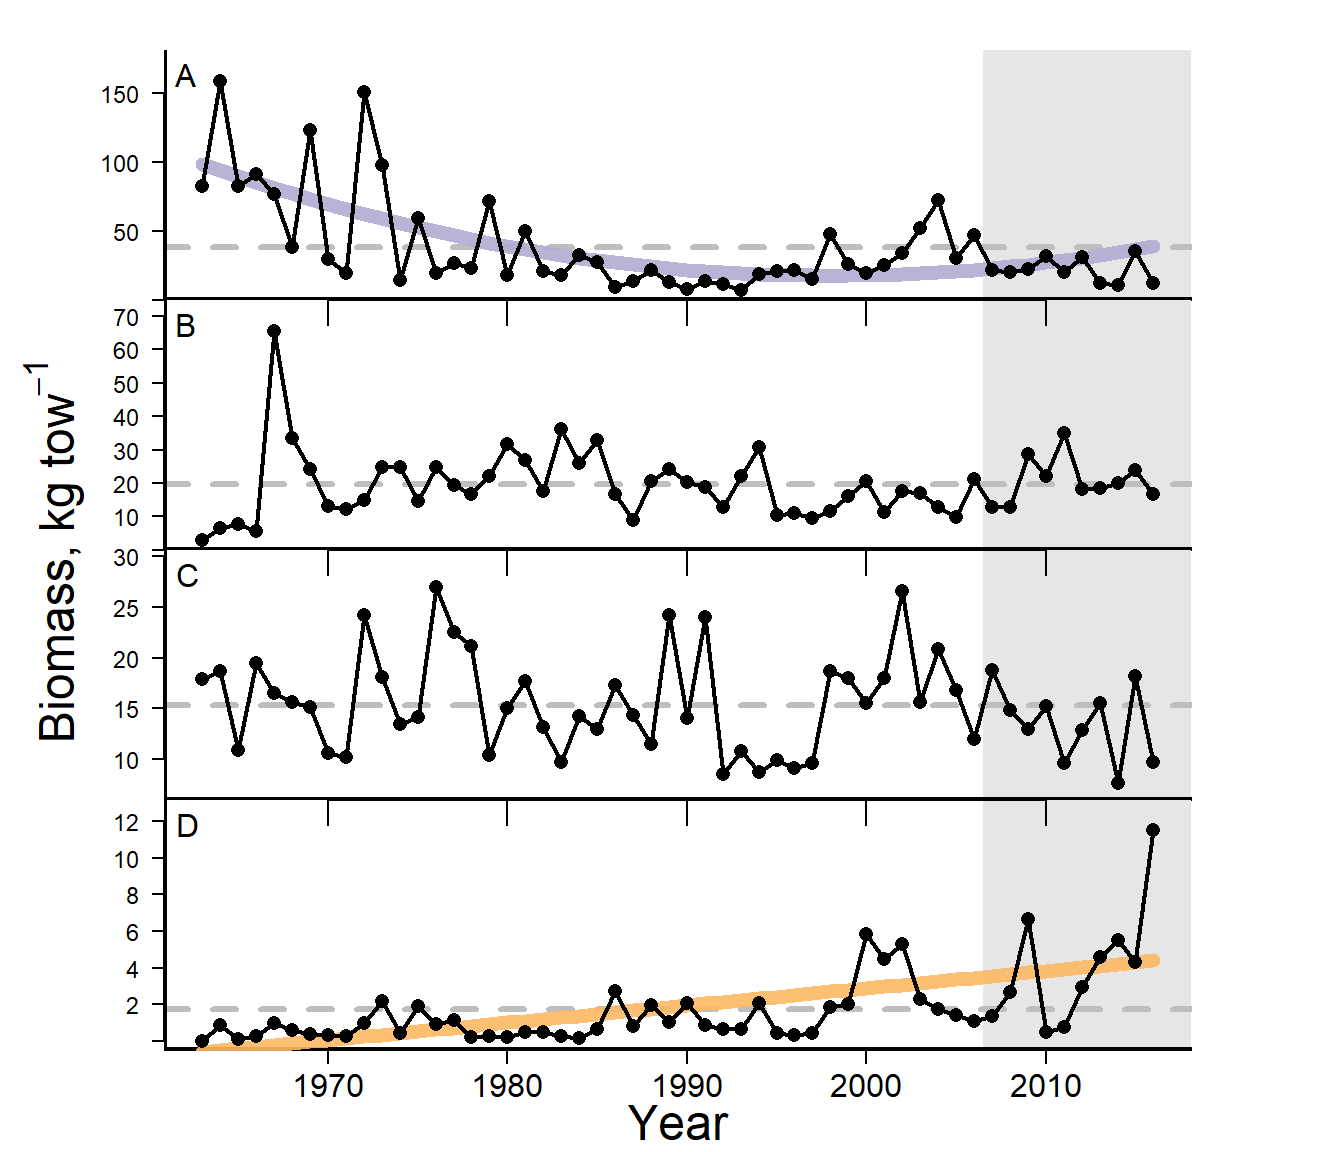
\includegraphics[width=0.5\linewidth]{C:/Users/kimberly.bastille/Desktop/tech-doc/imagesfall-survey-MAB-1} 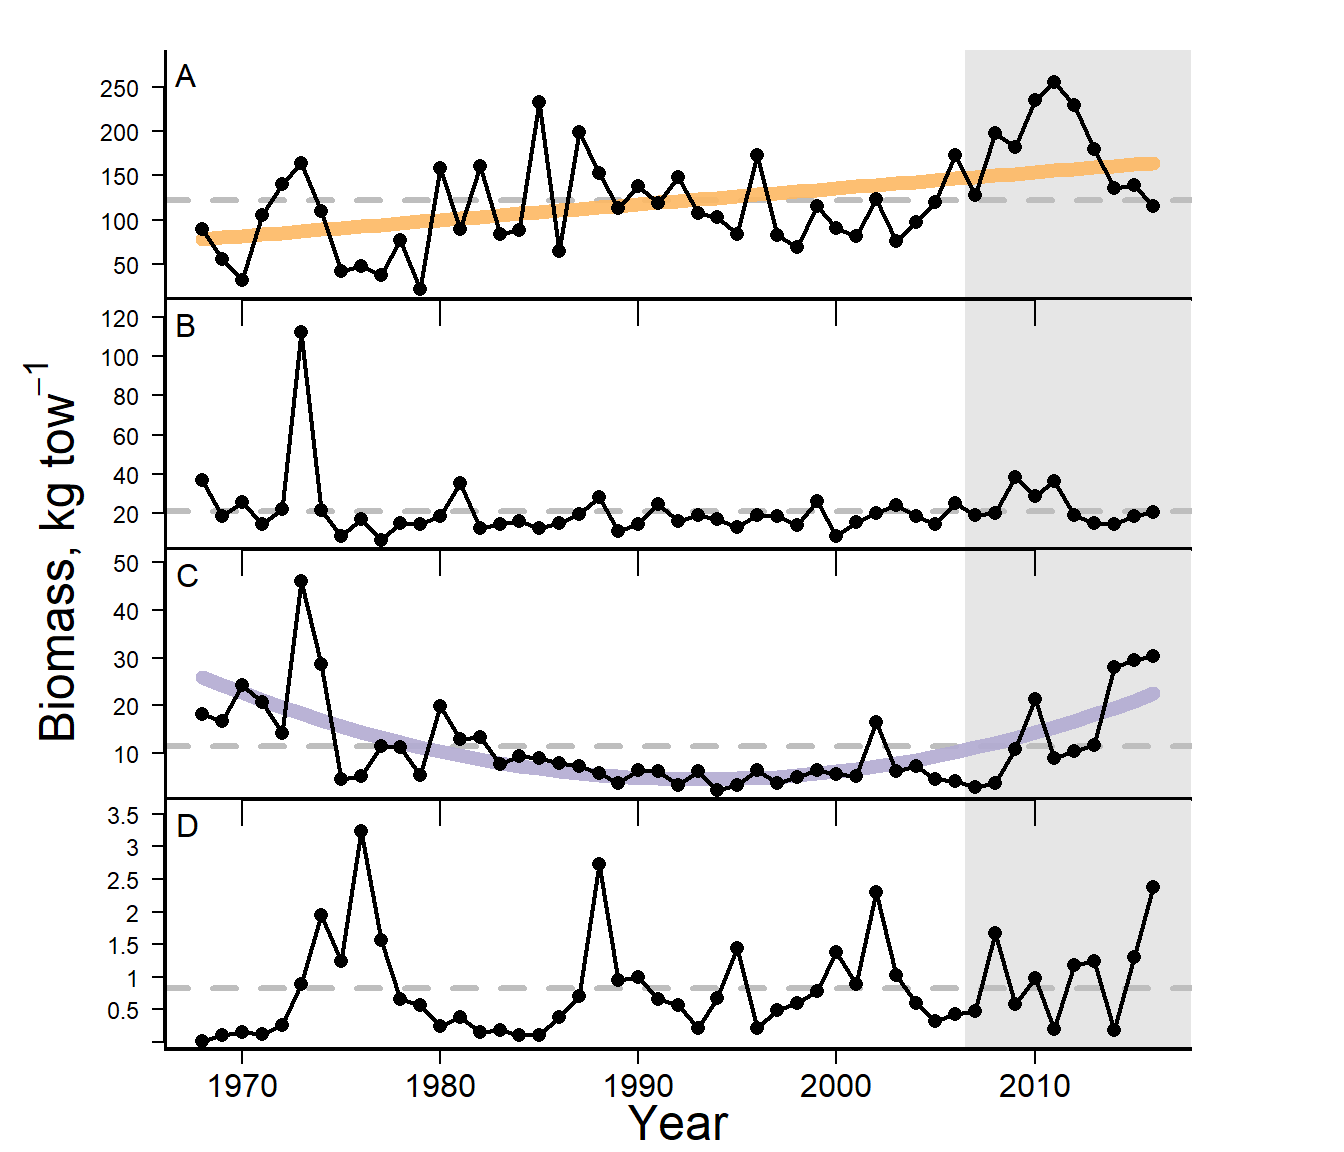
\includegraphics[width=0.5\linewidth]{C:/Users/kimberly.bastille/Desktop/tech-doc/imagesfall-survey-MAB-2} \caption{Fall (left) and spring (right) MAB Survey Biomass (A: Piscivore, B: Planktivore, C: Benthivore, D: Benthos).}\label{fig:fall-survey-MAB}
\end{figure}

\chapter{Thermal Habitat Projections}\label{thermal-habitat-projections}

\textbf{Description}: Species Thermal Habitat Projections

\textbf{Found in}: State of the Ecosystem - Gulf of Maine \& Georges
Bank (2018), State of the Ecosystem - Mid-Atlantic (2018)

\textbf{Indicator category}: Published methods

\textbf{Contributor(s)}: Vincent Saba

\textbf{Data steward}: Vincent Saba,
\href{mailto:vincent.saba@noaa.gov}{\nolinkurl{vincent.saba@noaa.gov}}

\textbf{Point of contact}: Vincent Saba,
\href{mailto:vincent.saba@noaa.gov}{\nolinkurl{vincent.saba@noaa.gov}}

\textbf{Public availability statement}: Source data are available to the
public. Model outputs for thermal habitat projections are available
\href{https://comet.nefsc.noaa.gov/erddap/info/index.html?page=1\&itemsPerPage=1000}{here}.

\section{Methods}\label{methods-31}

This indicator is based on work reported in Kleisner et al.
(\protect\hyperlink{ref-Kleisner2017}{2017}).

\subsection{Data sources}\label{data-sources-31}

\subsubsection{Global Climate Model
Projection}\label{global-climate-model-projection}

We used
\href{https://www.gfdl.noaa.gov/high-resolution-climate-modeling/}{NOAA
GFDL's CM2.6 simulation} consisting of (1) a 1860 pre-industrial
control, which brings the climate system into near-equilibrium with 1860
greenhouse gas concentrations, and (2) a transient climate response
(2xCO2) simulation where atmospheric CO2 is increased by 1\% per year,
which results in a doubling of CO2 after 70 years. The climate change
response from CM2.6 was based on the difference between these two
experimental runs. Refer to Saba et al.
(\protect\hyperlink{ref-Saba2016}{2016}) for further details.

\subsubsection{Modeling Changes in Suitable Thermal
Habitat}\label{modeling-changes-in-suitable-thermal-habitat}

The NOAA NEFSC U.S. Northeast Shelf (NES) bottom trawl survey, which has
been conducted for almost 50-years in the spring and fall, provides a
rich source of data on historical and current marine species
distribution, abundance, and habitat, as well as oceanographic
conditions (Azarovitz \protect\hyperlink{ref-Azarovitz1981}{1981}). The
survey was implemented to meet several objectives: (1) monitor trends in
abundance, biomass, and recruitment, (2) monitor the geographic
distribution of species, (3) monitor ecosystem changes, (4) monitor
changes in life history traits (e.g., trends in growth, longevity,
mortality, and maturation, and food habits), and (5) collect baseline
oceanographic and environmental data. These data can be leveraged for
exploring future changes in the patterns of abundance and distribution
of species in the region.

\subsection{Data analysis}\label{data-analysis-29}

\subsubsection{Global Climate Model
Projection}\label{global-climate-model-projection-1}

The CM2.6 80-year projections can be roughly assigned to a time period
by using the IPCC Representative Concentration Pathways (RCPs), which
describe four different 21st century pathways of anthropogenic
greenhouse gas emissions, air pollutant emissions, and land use (IPCC
\protect\hyperlink{ref-IPCC2014}{2014}). There are four RCPs, ranging
from a stringent mitigation scenario (RCP2.6), two intermediate
scenarios (RCP4.5 and RCP6.0), and one scenario with very high
greenhouse gas emissions (RCP8.5). For RCP8.5, the global average
temperature at the surface warms by 2C by approximately 2060-2070
relative to the 1986-2005 climatology (see Figure SPM.7a in
\href{https://www.ipcc.ch/pdf/assessment-report/ar5/wg1/WG1AR5_SPM_FINAL.pdf}{IPCC,
2013}). For CM2.6, the global average temperature warms by 2C by
approximately years 60-80 (see Fig. 1 in Winton et al.
(\protect\hyperlink{ref-winton_has_2014}{2014})). Therefore, the last 20
years of the transient climate response simulation roughly corresponds
to 2060-2080 of the RCP8.5 scenario.

Here, the monthly differences in surface and bottom temperatures
(`deltas') for spring (February-April) and fall (September- November)
are added to an average annual temperature climatology for spring and
fall, respectively, derived from observed surface and bottom
temperatures to produce an 80-year time series of future bottom and
surface temperatures in both seasons. The observed temperatures come
from the NEFSC spring and fall bottom trawl surveys conducted from 1968
to 2013 and represent approximately 30,000 observations over the time
series.

\subsubsection{Modeling Changes in Suitable Thermal
Habitat}\label{modeling-changes-in-suitable-thermal-habitat-1}

We modeled individual species thermal habitat across the whole U.S. NES
and not by sub-region because we did not want to assume that species
would necessarily maintain these assemblages in the future. Indeed, the
goal here is to determine future patterns of thermal habitat
availability for species on the U.S. NES in more broad terms. We fit one
GAM based on both spring and fall data (i.e., an annual model as opposed
to separate spring and fall models) and use it to project potential
changes in distribution and magnitude of biomass separately for each
season for each species. By creating a single annual model based on
temperature data from both spring and fall, we ensure that the full
thermal envelope of each species is represented. For example, if a
species with a wide thermal tolerance has historically been found in
cooler waters in the spring, and in warmer waters in the fall, an annual
model will ensure that if there are warmer waters in the spring in the
future, that species will have the potential to inhabit those areas.
Additionally, because the trawl survey data are subject to many zero
observations, we use delta-lognormal GAMs (Wood
\protect\hyperlink{ref-Wood2011a}{2011}), which model presence-absence
separately from logged positive observations. The response variables in
each of the GAMs are presence/absence and logged positive biomass of
each assemblage or individual species, respectively. A binomial link
function is used in the presence/absence models and a Gaussian link
function is used in the models with logged positive biomass. The
predictor variables are surface and bottom temperature and depth (all
measured by the survey at each station), fit with penalized regression
splines, and survey stratum, which accounts for differences in regional
habitat quality across the survey region. Stratum may be considered to
account for additional information not explicitly measured by the survey
(e.g., bottom rugosity). Predictions of species abundance are calculated
as the product of the predictions from the presence-absence model, the
exponentiated predictions from the logged positive biomass model, and a
correction factor to account for the retransformation bias associated
with the log transformation (Duan
\protect\hyperlink{ref-Duan1983}{1983}; and see Pinsky et al.
\protect\hyperlink{ref-Pinsky2013}{2013}).

We calculated the suitable thermal habitat both in terms of changes in
`suitable thermal abundance', defined as the species density possible
given appropriate temperature, depth and bathymetric conditions, and
changes in `suitable thermal area', defined as the size of the physical
area potentially occupied by a species given appropriate temperature,
depth and bathymetric conditions. Suitable thermal abundance is
determined from the predictions from the GAMs (i.e., a prediction of
biomass). However, this quantity should not be interpreted directly as a
change in future abundance or biomass, but instead as the potential
abundance of a species in the future given changes in temperature and
holding all else (e.g., fishing effort, species interactions,
productivity, etc.) constant. Suitable thermal area is determined as a
change in the suitable area that a species distribution occupies in the
future and is derived from the area of the kernel density of the
distribution. To ensure that the estimates are conservative, we select
all points with values greater than one standard deviation above the
mean. We then compute the area of these kernels using the gArea function
from the `rgeos' package in R (Bivand et al.
\protect\hyperlink{ref-Bivand2011}{2011}).

\subsection{Plotting}\label{plotting-23}

\begin{figure}
\centering
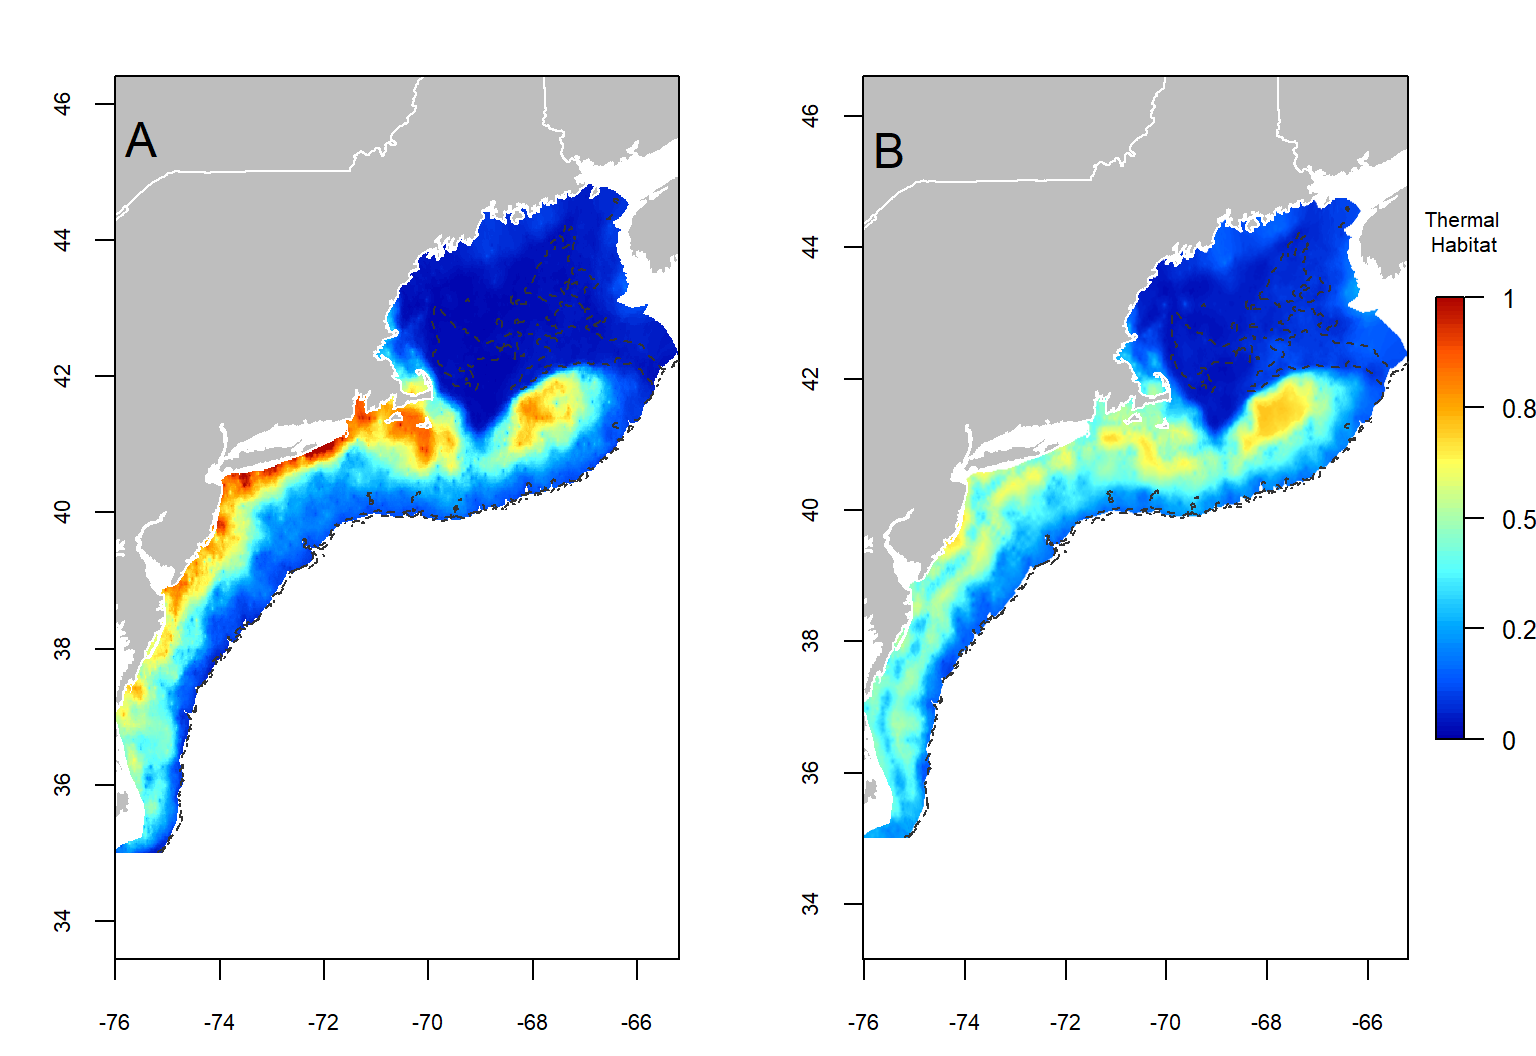
\includegraphics{C:/Users/kimberly.bastille/Desktop/tech-doc/imagesth-maps-1.pdf}
\caption{\label{fig:th-maps}Current thermal habitat estimate (A), and 20-40
year thermal habitat projection (B) for summer flounder on the Northeast
Continental Shelf.}
\end{figure}

\textbf{Note}: The thermal habitat model output for all species
presented in State of the Ecosystem reports is accessible through the
\href{https://comet.nefsc.noaa.gov/erddap/info/index.html?page=1\&itemsPerPage=1000}{NEFSC
ERDDAP server}.

\chapter{Trend Analysis}\label{trend-analysis}

\textbf{Description}: Time series trend analysis

\textbf{Found in}: State of the Ecosystem - Gulf of Maine \& Georges
Bank (2018, 2019), State of the Ecosystem - Mid-Atlantic (2018, 2019)

\textbf{Indicator category}: Extensive analysis, not yet published

\textbf{Contributor(s)}: Sean Hardison, Charles Perretti, Geret DePiper

\textbf{Data steward}: NA

\textbf{Point of contact}: Sean Hardison,
\href{mailto:sean.hardison@noaa.gov}{\nolinkurl{sean.hardison@noaa.gov}}

\textbf{Public availability statement}: NA

\section{Methods}\label{methods-32}

Summarizing trends for ecosystem indicators is desirable, but the power
of statistical tests to detect a trend is hampered by low sample size
and autocorrelated observations (see Nicholson and Jennings
\protect\hyperlink{ref-Nicholson2004}{2004}; Wagner et al.
\protect\hyperlink{ref-Wagner2013}{2013}; Storch
\protect\hyperlink{ref-VonStorch1999a}{1999}). Prior to 2018, time
series indicators in State of the Ecosystem reports were presented with
trend lines based on a Mann-Kendall test for monotonic trends to test
significance (p \textless{} 0.05) of both long term (full time series)
and recent (2007--2016) trends, although not all time series were
considered for trend analysis due to limited series lengths. There was
also concern that a Mann-Kendall test would not account for any
autocorrelation present in SOE indicators.

In a simulation study (Hardison et al.
\protect\hyperlink{ref-hardison2019}{2019}), we explored the effect of
time series length and autocorrelation strength on statistical power of
three trend detection methods: a generalized least squares model
selection approach, the Mann-Kendall test, and Mann-Kendall test with
trend-free pre-whitening. Methods were applied to simulated time series
of varying trend and autocorrelation strengths. Overall, when sample
size was low (N = 10) there were high rates of false trend detection,
and similarly, low rates of true trend detection. Both of these forms of
error were further amplified by autocorrelation in the trend residuals.
Based on these findings, we selected a minimum series length of N = 30
for indicator time series before assessing trend.

We also chose to use a GLS model selection (GLS-MS) approach to evaluate
indicator trends in the 2018 (and future) State of the Ecosystem
reports, as this approach performed best overall in the simulation
study. GLS-MS also allowed for both linear and quadratic model fits and
quantification of uncertainty in trend estimates. The model selection
procedure for the GLS approach fits four models to each time series and
selects the best fitting model using AICc. The models are, 1) linear
trend with uncorrelated residuals, 2) linear trend with correlated
residuals, 3) quadratic trend with uncorrelated residuals, and 4)
quadratic trend with correlated residuals. I.e., the models are of the
form

\[ Y_t = \alpha_0 + \alpha_1X_t + \alpha_2X_t^2 + \epsilon_t\]
\[\epsilon_t = \rho\epsilon_{t-1} + \omega_t\]

\[w_t \sim N(0, \sigma^2)\]

Where \(Y_t\) is the observation in time \(t\), \(X_t\) is the time
index, \(\epsilon_t\) is the residual in time \(t\), and \(\omega_t\) is
a normally distributed random variable. Setting \(\alpha_2 = 0\) yields
the linear trend model, and \(\rho = 0\) yields the uncorrelated
residuals model.

The best fit model was tested against the null hypothesis of no trend
through a likelihood ratio test (p \textless{} 0.05). All models were
fit using the R package \emph{nlme} (Pinheiro et al.
\protect\hyperlink{ref-Pinheiro2017}{2017}) and AICc was calculated
using the R package \emph{AICcmodavg} (Mazerolle
\protect\hyperlink{ref-Mazerolle2017a}{2017}). In SOE time series
figures, significant positive trends were colored orange, and negative
trends purple.

\subsection{Data source(s)}\label{data-sources-32}

NA

\subsection{Data extraction}\label{data-extraction-24}

NA

\subsection{Data analysis}\label{data-analysis-30}

\begin{Shaded}
\begin{Highlighting}[]
\CommentTok{#R packages}
\KeywordTok{library}\NormalTok{(dplyr)}
\KeywordTok{library}\NormalTok{(nlme)}
\KeywordTok{library}\NormalTok{(AICcmodavg)}
\KeywordTok{library}\NormalTok{(data.table)}
\end{Highlighting}
\end{Shaded}

\begin{Shaded}
\begin{Highlighting}[]
\CommentTok{# data.dir <- "./data"}
\CommentTok{# load(file.path(data.dir, "SOE_data_2018.Rdata"))}

\CommentTok{#--------------------------------GLS Model Selection-----------------------------#}
\NormalTok{fit_lm <-}\StringTok{ }\ControlFlowTok{function}\NormalTok{(dat) \{}

\NormalTok{  constant_norm <-}
\StringTok{    }\NormalTok{nlme}\OperatorTok{::}\KeywordTok{gls}\NormalTok{(series }\OperatorTok{~}\StringTok{ }\DecValTok{1}\NormalTok{, }
              \DataTypeTok{data =}\NormalTok{ dat)}
  
\NormalTok{  constant_ar1 <-}
\StringTok{    }\KeywordTok{try}\NormalTok{(nlme}\OperatorTok{::}\KeywordTok{gls}\NormalTok{(series }\OperatorTok{~}\StringTok{ }\DecValTok{1}\NormalTok{,}
                  \DataTypeTok{data =}\NormalTok{ dat,}
                  \DataTypeTok{correlation =}\NormalTok{ nlme}\OperatorTok{::}\KeywordTok{corAR1}\NormalTok{(}\DataTypeTok{form =} \OperatorTok{~}\NormalTok{time)))}
  \ControlFlowTok{if}\NormalTok{ (}\KeywordTok{class}\NormalTok{(constant_ar1) }\OperatorTok{==}\StringTok{ "try-error"}\NormalTok{)\{}
    \KeywordTok{return}\NormalTok{(best_lm <-}\StringTok{ }\KeywordTok{data.frame}\NormalTok{(}\DataTypeTok{model =} \OtherTok{NA}\NormalTok{,}
                                 \DataTypeTok{aicc  =} \OtherTok{NA}\NormalTok{,}
                                 \DataTypeTok{coefs..Intercept =} \OtherTok{NA}\NormalTok{,}
                                 \DataTypeTok{coefs.time =} \OtherTok{NA}\NormalTok{,}
                                 \DataTypeTok{coefs.time2 =} \OtherTok{NA}\NormalTok{,}
                                 \DataTypeTok{pval =} \OtherTok{NA}\NormalTok{)) }
\NormalTok{  \} }
  
  
  
  \CommentTok{# Linear model with normal error}
\NormalTok{  linear_norm <-}\StringTok{ }
\StringTok{    }\NormalTok{nlme}\OperatorTok{::}\KeywordTok{gls}\NormalTok{(series }\OperatorTok{~}\StringTok{ }\NormalTok{time, }
              \DataTypeTok{data =}\NormalTok{ dat)}
  
  \CommentTok{# Linear model with AR1 error}
\NormalTok{  linear_ar1 <-}\StringTok{ }
\StringTok{    }\KeywordTok{try}\NormalTok{(nlme}\OperatorTok{::}\KeywordTok{gls}\NormalTok{(series }\OperatorTok{~}\StringTok{ }\NormalTok{time, }
                  \DataTypeTok{data =}\NormalTok{ dat,}
                  \DataTypeTok{correlation =}\NormalTok{ nlme}\OperatorTok{::}\KeywordTok{corAR1}\NormalTok{(}\DataTypeTok{form =} \OperatorTok{~}\NormalTok{time)))}
  \ControlFlowTok{if}\NormalTok{ (}\KeywordTok{class}\NormalTok{(linear_ar1) }\OperatorTok{==}\StringTok{ "try-error"}\NormalTok{)\{}
    \KeywordTok{return}\NormalTok{(best_lm <-}\StringTok{ }\KeywordTok{data.frame}\NormalTok{(}\DataTypeTok{model =} \OtherTok{NA}\NormalTok{,}
                                 \DataTypeTok{aicc  =} \OtherTok{NA}\NormalTok{,}
                                 \DataTypeTok{coefs..Intercept =} \OtherTok{NA}\NormalTok{,}
                                 \DataTypeTok{coefs.time =} \OtherTok{NA}\NormalTok{,}
                                 \DataTypeTok{coefs.time2 =} \OtherTok{NA}\NormalTok{,}
                                 \DataTypeTok{pval =} \OtherTok{NA}\NormalTok{))}
    
\NormalTok{  \}}
  
  \CommentTok{# Polynomial model with normal error}
\NormalTok{  dat}\OperatorTok{$}\NormalTok{time2 <-}\StringTok{ }\NormalTok{dat}\OperatorTok{$}\NormalTok{time}\OperatorTok{^}\DecValTok{2}
\NormalTok{  poly_norm <-}\StringTok{ }
\StringTok{    }\NormalTok{nlme}\OperatorTok{::}\KeywordTok{gls}\NormalTok{(series }\OperatorTok{~}\StringTok{ }\NormalTok{time }\OperatorTok{+}\StringTok{ }\NormalTok{time2, }
              \DataTypeTok{data =}\NormalTok{ dat)}
  
  \CommentTok{# Polynomial model with AR1 error}
\NormalTok{  poly_ar1 <-}\StringTok{ }
\StringTok{    }\KeywordTok{try}\NormalTok{(nlme}\OperatorTok{::}\KeywordTok{gls}\NormalTok{(series }\OperatorTok{~}\StringTok{ }\NormalTok{time }\OperatorTok{+}\StringTok{ }\NormalTok{time2, }
                  \DataTypeTok{data =}\NormalTok{ dat,}
                  \DataTypeTok{correlation =}\NormalTok{ nlme}\OperatorTok{::}\KeywordTok{corAR1}\NormalTok{(}\DataTypeTok{form =} \OperatorTok{~}\NormalTok{time)))}
  \ControlFlowTok{if}\NormalTok{ (}\KeywordTok{class}\NormalTok{(poly_ar1) }\OperatorTok{==}\StringTok{ "try-error"}\NormalTok{)\{}
    \KeywordTok{return}\NormalTok{(best_lm <-}\StringTok{ }\KeywordTok{data.frame}\NormalTok{(}\DataTypeTok{model =} \OtherTok{NA}\NormalTok{,}
                                 \DataTypeTok{aicc  =} \OtherTok{NA}\NormalTok{,}
                                 \DataTypeTok{coefs..Intercept =} \OtherTok{NA}\NormalTok{,}
                                 \DataTypeTok{coefs.time =} \OtherTok{NA}\NormalTok{,}
                                 \DataTypeTok{coefs.time2 =} \OtherTok{NA}\NormalTok{,}
                                 \DataTypeTok{pval =} \OtherTok{NA}\NormalTok{))}
    
\NormalTok{  \}}
  
  \CommentTok{# Calculate AICs for all models}
\NormalTok{  df_aicc <-}
\StringTok{    }\KeywordTok{data.frame}\NormalTok{(}\DataTypeTok{model =} \KeywordTok{c}\NormalTok{(}\StringTok{"poly_norm"}\NormalTok{,}
                         \StringTok{"poly_ar1"}\NormalTok{,}
                         \StringTok{"linear_norm"}\NormalTok{,}
                         \StringTok{"linear_ar1"}\NormalTok{),}
               \DataTypeTok{aicc  =} \KeywordTok{c}\NormalTok{(}\KeywordTok{AICc}\NormalTok{(poly_norm),}
                         \KeywordTok{AICc}\NormalTok{(poly_ar1),}
                         \KeywordTok{AICc}\NormalTok{(linear_norm),}
                         \KeywordTok{AICc}\NormalTok{(linear_ar1)),}
               \DataTypeTok{coefs =} \KeywordTok{rbind}\NormalTok{(}\KeywordTok{coef}\NormalTok{(poly_norm),}
                             \KeywordTok{coef}\NormalTok{(poly_ar1),}
                             \KeywordTok{c}\NormalTok{(}\KeywordTok{coef}\NormalTok{(linear_norm), }\OtherTok{NA}\NormalTok{),}
                             \KeywordTok{c}\NormalTok{(}\KeywordTok{coef}\NormalTok{(linear_ar1),  }\OtherTok{NA}\NormalTok{)),}
               \CommentTok{# Calculate overall signifiance (need to use}
               \CommentTok{# ML not REML for this)}
               \DataTypeTok{pval =} \KeywordTok{c}\NormalTok{(}\KeywordTok{anova}\NormalTok{(}\KeywordTok{update}\NormalTok{(constant_norm, }\DataTypeTok{method =} \StringTok{"ML"}\NormalTok{),}
                              \KeywordTok{update}\NormalTok{(poly_norm, }\DataTypeTok{method =} \StringTok{"ML"}\NormalTok{))}\OperatorTok{$}\StringTok{`}\DataTypeTok{p-value}\StringTok{`}\NormalTok{[}\DecValTok{2}\NormalTok{],}
                        \KeywordTok{anova}\NormalTok{(}\KeywordTok{update}\NormalTok{(constant_ar1, }\DataTypeTok{method =} \StringTok{"ML"}\NormalTok{),}
                              \KeywordTok{update}\NormalTok{(poly_ar1, }\DataTypeTok{method =} \StringTok{"ML"}\NormalTok{))}\OperatorTok{$}\StringTok{`}\DataTypeTok{p-value}\StringTok{`}\NormalTok{[}\DecValTok{2}\NormalTok{],}
                        \KeywordTok{anova}\NormalTok{(}\KeywordTok{update}\NormalTok{(constant_norm, }\DataTypeTok{method =} \StringTok{"ML"}\NormalTok{),}
                              \KeywordTok{update}\NormalTok{(linear_norm, }\DataTypeTok{method =} \StringTok{"ML"}\NormalTok{))}\OperatorTok{$}\StringTok{`}\DataTypeTok{p-value}\StringTok{`}\NormalTok{[}\DecValTok{2}\NormalTok{],}
                        \KeywordTok{anova}\NormalTok{(}\KeywordTok{update}\NormalTok{(constant_ar1, }\DataTypeTok{method =} \StringTok{"ML"}\NormalTok{),}
                              \KeywordTok{update}\NormalTok{(linear_ar1, }\DataTypeTok{method =} \StringTok{"ML"}\NormalTok{))}\OperatorTok{$}\StringTok{`}\DataTypeTok{p-value}\StringTok{`}\NormalTok{[}\DecValTok{2}\NormalTok{]))}
  
\NormalTok{  best_lm <-}
\StringTok{    }\NormalTok{df_aicc }\OperatorTok
\StringTok{    }\NormalTok{dplyr}\OperatorTok{::}\KeywordTok{filter}\NormalTok{(aicc }\OperatorTok{==}\StringTok{ }\KeywordTok{min}\NormalTok{(aicc))}
  
  
  \ControlFlowTok{if}\NormalTok{ (best_lm}\OperatorTok{$}\NormalTok{model }\OperatorTok{==}\StringTok{ "poly_norm"}\NormalTok{) \{}
\NormalTok{    model <-}\StringTok{ }\NormalTok{poly_norm}
\NormalTok{  \} }\ControlFlowTok{else} \ControlFlowTok{if}\NormalTok{ (best_lm}\OperatorTok{$}\NormalTok{model }\OperatorTok{==}\StringTok{ "poly_ar1"}\NormalTok{) \{}
\NormalTok{    model <-}\StringTok{ }\NormalTok{poly_ar1}
\NormalTok{  \} }\ControlFlowTok{else} \ControlFlowTok{if}\NormalTok{ (best_lm}\OperatorTok{$}\NormalTok{model }\OperatorTok{==}\StringTok{ "linear_norm"}\NormalTok{) \{}
\NormalTok{    model <-}\StringTok{ }\NormalTok{linear_norm}
\NormalTok{  \} }\ControlFlowTok{else} \ControlFlowTok{if}\NormalTok{ (best_lm}\OperatorTok{$}\NormalTok{model }\OperatorTok{==}\StringTok{ "linear_ar1"}\NormalTok{) \{}
\NormalTok{    model <-}\StringTok{ }\NormalTok{linear_ar1}
\NormalTok{  \}}
  
  \KeywordTok{return}\NormalTok{(}\KeywordTok{list}\NormalTok{(}\DataTypeTok{p =}\NormalTok{ best_lm}\OperatorTok{$}\NormalTok{pval,}
              \DataTypeTok{model =}\NormalTok{ model))}
\NormalTok{\}}

\CommentTok{#-------------------------------------Plotting code------------------------------------#}
\NormalTok{soe.plot <-}\StringTok{ }\ControlFlowTok{function}\NormalTok{(data, x.var, y.var, }\DataTypeTok{x.label =} \StringTok{''}\NormalTok{, }\DataTypeTok{y.label =} \StringTok{''}\NormalTok{, }\DataTypeTok{tol =} \FloatTok{0.1}\NormalTok{,}
                     \DataTypeTok{x.start =} \OtherTok{NA}\NormalTok{, }\DataTypeTok{x.end =} \OtherTok{NA}\NormalTok{, }\DataTypeTok{end.start =} \DecValTok{2008}\NormalTok{, }\DataTypeTok{bg.col =}\NormalTok{ background, }\DataTypeTok{mean_line =}\NormalTok{ T,}
                     \DataTypeTok{end.col =}\NormalTok{ recent, }\DataTypeTok{stacked =} \OtherTok{NA}\NormalTok{, }\DataTypeTok{x.line =} \FloatTok{2.5}\NormalTok{, }\DataTypeTok{y.line =} \FloatTok{3.5}\NormalTok{, }\DataTypeTok{scale.axis =} \DecValTok{1}\NormalTok{,}
                     \DataTypeTok{rel.y.num =} \FloatTok{1.5}\NormalTok{, }\DataTypeTok{rel.y.text =} \FloatTok{1.5}\NormalTok{, }\DataTypeTok{suppressAxis =} \OtherTok{FALSE}\NormalTok{,}\DataTypeTok{status  =}\NormalTok{ F,}\DataTypeTok{anomaly =}\NormalTok{ F,}
                     \DataTypeTok{endshade =} \OtherTok{TRUE}\NormalTok{, }\DataTypeTok{full.trend =} \OtherTok{TRUE}\NormalTok{, }\DataTypeTok{point.cex =} \FloatTok{1.5}\NormalTok{, }\DataTypeTok{lwd =} \DecValTok{2}\NormalTok{, }\DataTypeTok{ymax =} \OtherTok{TRUE}\NormalTok{,}\DataTypeTok{ymin =} \OtherTok{TRUE}\NormalTok{,}
                     \DataTypeTok{y.upper =}\NormalTok{ y.upper, }\DataTypeTok{y.lower =}\NormalTok{ y.lower, }\DataTypeTok{extra =} \OtherTok{FALSE}\NormalTok{, }\DataTypeTok{x.var2 =}\NormalTok{ x.var2, }\DataTypeTok{y.var2 =}\NormalTok{ y.var2,}
                     \DataTypeTok{line.forward =} \OtherTok{FALSE}\NormalTok{, }\DataTypeTok{mean_line.2 =}\NormalTok{ T, }\DataTypeTok{cex.stacked =} \DecValTok{1}\NormalTok{, }\DataTypeTok{website =}\NormalTok{ T) \{}
  

  \CommentTok{#Select Data}
\NormalTok{  x <-}\StringTok{ }\NormalTok{data[Var }\OperatorTok{==}\StringTok{ }\NormalTok{y.var, ]}
\NormalTok{  x <-}\StringTok{ }\NormalTok{x[}\KeywordTok{order}\NormalTok{(x[, }\KeywordTok{get}\NormalTok{(x.var)]), ]}
  \KeywordTok{setnames}\NormalTok{(x, x.var, }\StringTok{'X'}\NormalTok{)}
  
  \CommentTok{#Set common time step if necessary}
  \ControlFlowTok{if}\NormalTok{(}\KeywordTok{is.na}\NormalTok{(x.start)) x.start <-}\StringTok{ }\KeywordTok{min}\NormalTok{(x[, X])}
  \ControlFlowTok{if}\NormalTok{(}\KeywordTok{is.na}\NormalTok{(x.end))   x.end   <-}\StringTok{ }\KeywordTok{max}\NormalTok{(x[, X])}
\NormalTok{  x <-}\StringTok{ }\NormalTok{x[X }\OperatorTok{>=}\StringTok{ }\NormalTok{x.start, ]}
  
  \CommentTok{#Set up plot parameters}
  \ControlFlowTok{if}\NormalTok{ (ymax }\OperatorTok{==}\StringTok{ }\OtherTok{TRUE}\NormalTok{)\{}
\NormalTok{    y.max <-}\StringTok{ }\KeywordTok{max}\NormalTok{(x[, Value]) }\OperatorTok{+}\StringTok{ }\NormalTok{tol }\OperatorTok{*}\StringTok{ }\KeywordTok{max}\NormalTok{(x[, Value])}
\NormalTok{  \} }\ControlFlowTok{else}\NormalTok{ \{}
\NormalTok{    y.max <-}\StringTok{ }\KeywordTok{as.numeric}\NormalTok{(y.upper)}
\NormalTok{  \}}
  
  \ControlFlowTok{if}\NormalTok{ (ymin }\OperatorTok{==}\StringTok{ }\OtherTok{TRUE}\NormalTok{)\{}
\NormalTok{    y.min <-}\StringTok{ }\KeywordTok{min}\NormalTok{(x[, Value]) }\OperatorTok{-}\StringTok{ }\NormalTok{tol }\OperatorTok{*}\StringTok{ }\KeywordTok{abs}\NormalTok{(}\KeywordTok{min}\NormalTok{(x[, Value]))}
\NormalTok{  \} }\ControlFlowTok{else} \ControlFlowTok{if}\NormalTok{ (ymin }\OperatorTok{==}\StringTok{ }\OtherTok{FALSE}\NormalTok{)\{}
\NormalTok{    y.min <-}\StringTok{ }\KeywordTok{as.numeric}\NormalTok{(y.lower)}
\NormalTok{  \}}
  
\NormalTok{  y.mean <-}\StringTok{ }\KeywordTok{mean}\NormalTok{(x[, Value])}
\NormalTok{  y.sd <-}\StringTok{ }\KeywordTok{sd}\NormalTok{(x[, Value])}
  
  \CommentTok{#Plot blank plot}
  \KeywordTok{plot}\NormalTok{(x[X }\OperatorTok{>=}\StringTok{ }\NormalTok{x.start, }\KeywordTok{list}\NormalTok{(X, Var)], }\DataTypeTok{xlim =} \KeywordTok{c}\NormalTok{(x.start, x.end),}
       \DataTypeTok{ylim =} \KeywordTok{c}\NormalTok{(y.min,y.max), }\DataTypeTok{xlab =} \StringTok{''}\NormalTok{, }\DataTypeTok{ylab =} \StringTok{''}\NormalTok{, }\DataTypeTok{axes =}\NormalTok{ F, }\DataTypeTok{ty =} \StringTok{'n'}\NormalTok{)}


  \CommentTok{#Add background}
\NormalTok{  u <-}\StringTok{ }\KeywordTok{par}\NormalTok{(}\StringTok{'usr'}\NormalTok{)}
  \KeywordTok{rect}\NormalTok{(u[}\DecValTok{1}\NormalTok{], u[}\DecValTok{3}\NormalTok{], u[}\DecValTok{2}\NormalTok{], u[}\DecValTok{4}\NormalTok{], }\DataTypeTok{border =} \OtherTok{NA}\NormalTok{, }\DataTypeTok{col =}\NormalTok{ bg.col)}
  
  \CommentTok{#Add end period shading}
  \ControlFlowTok{if}\NormalTok{ (endshade }\OperatorTok{==}\StringTok{ }\OtherTok{TRUE}\NormalTok{)\{}
    \KeywordTok{rect}\NormalTok{(end.start }\OperatorTok{-}\StringTok{ }\FloatTok{0.5}\NormalTok{, u[}\DecValTok{3}\NormalTok{], u[}\DecValTok{2}\NormalTok{], u[}\DecValTok{4}\NormalTok{], }\DataTypeTok{border =} \OtherTok{NA}\NormalTok{, }\DataTypeTok{col =}\NormalTok{ end.col)}
\NormalTok{  \}}
  
  \CommentTok{#Add mean line}
  \ControlFlowTok{if}\NormalTok{ (anomaly }\OperatorTok{==}\StringTok{ }\NormalTok{F)\{}
      \ControlFlowTok{if}\NormalTok{ (mean_line }\OperatorTok{==}\StringTok{ }\OtherTok{TRUE}\NormalTok{)\{}
      \KeywordTok{abline}\NormalTok{(}\DataTypeTok{h =}\NormalTok{ y.mean, }\DataTypeTok{col =} \StringTok{'grey'}\NormalTok{, }\DataTypeTok{lwd =} \DecValTok{3}\NormalTok{, }\DataTypeTok{lty =} \DecValTok{2}\NormalTok{)}
\NormalTok{      \} }
\NormalTok{  \} }\ControlFlowTok{else} \ControlFlowTok{if}\NormalTok{ (anomaly }\OperatorTok{==}\StringTok{ }\OtherTok{TRUE}\NormalTok{)\{}
      \KeywordTok{abline}\NormalTok{(}\DataTypeTok{h =} \DecValTok{0}\NormalTok{, }\DataTypeTok{col =} \StringTok{'grey'}\NormalTok{, }\DataTypeTok{lwd =} \DecValTok{3}\NormalTok{, }\DataTypeTok{lty =} \DecValTok{2}\NormalTok{)}
\NormalTok{  \}}
  
  \CommentTok{#Add x y lines}
  \KeywordTok{abline}\NormalTok{(}\DataTypeTok{h =}\NormalTok{ u[}\DecValTok{3}\NormalTok{], }\DataTypeTok{lwd=}\DecValTok{3}\NormalTok{)}
  \KeywordTok{abline}\NormalTok{(}\DataTypeTok{v =}\NormalTok{ u[}\DecValTok{1}\NormalTok{], }\DataTypeTok{lwd=}\DecValTok{3}\NormalTok{)}
  
  \CommentTok{#Add data points/lines}
  \KeywordTok{points}\NormalTok{(x[, }\KeywordTok{list}\NormalTok{(X, Value)], }\DataTypeTok{pch =} \DecValTok{16}\NormalTok{, }\DataTypeTok{cex =}\NormalTok{ point.cex)}
  \KeywordTok{lines}\NormalTok{( x[, }\KeywordTok{list}\NormalTok{(X, Value)], }\DataTypeTok{lwd =}\NormalTok{ lwd)}
  
  \CommentTok{#extra lines}
  \ControlFlowTok{if}\NormalTok{ (extra }\OperatorTok{==}\StringTok{ }\OtherTok{TRUE}\NormalTok{)\{}
\NormalTok{    x2 <-}\StringTok{ }\NormalTok{data[Var }\OperatorTok{==}\StringTok{ }\NormalTok{y.var2, ]}
\NormalTok{    x2 <-}\StringTok{ }\NormalTok{x2[}\KeywordTok{order}\NormalTok{(x2[, }\KeywordTok{get}\NormalTok{(x.var2)]), ]}
    \KeywordTok{setnames}\NormalTok{(x2, x.var2, }\StringTok{'X2'}\NormalTok{)}
\NormalTok{    x2 <-}\StringTok{ }\NormalTok{x2[X2 }\OperatorTok{>=}\StringTok{ }\NormalTok{x.start, ]}
    \ControlFlowTok{if}\NormalTok{ (mean_line.}\DecValTok{2} \OperatorTok{==}\StringTok{ }\OtherTok{TRUE}\NormalTok{)\{}
     \KeywordTok{abline}\NormalTok{(}\DataTypeTok{h =} \KeywordTok{mean}\NormalTok{(x2[, Value]), }\DataTypeTok{col =} \StringTok{'lightcoral'}\NormalTok{, }\DataTypeTok{lwd =} \DecValTok{3}\NormalTok{, }\DataTypeTok{lty =} \DecValTok{2}\NormalTok{) }
\NormalTok{    \}}
    \KeywordTok{points}\NormalTok{(x2[, }\KeywordTok{list}\NormalTok{(X2, Value)], }\DataTypeTok{pch =} \DecValTok{16}\NormalTok{, }\DataTypeTok{cex =}\NormalTok{ point.cex, }\DataTypeTok{col =} \StringTok{"indianred"}\NormalTok{)}
    \KeywordTok{lines}\NormalTok{( x2[, }\KeywordTok{list}\NormalTok{(X2, Value)], }\DataTypeTok{lwd =}\NormalTok{ lwd, }\DataTypeTok{col =} \StringTok{"indianred"}\NormalTok{)}
\NormalTok{    \}}
    
  
  \CommentTok{#Add axis}
  \ControlFlowTok{if}\NormalTok{ (suppressAxis }\OperatorTok{==}\StringTok{ }\OtherTok{FALSE}\NormalTok{)\{}
    \ControlFlowTok{if}\NormalTok{(}\KeywordTok{is.na}\NormalTok{(stacked)) }\KeywordTok{axis}\NormalTok{(}\DecValTok{1}\NormalTok{, }\DataTypeTok{cex.axis =} \DecValTok{1}\NormalTok{)}
    \ControlFlowTok{if}\NormalTok{(}\OperatorTok{!}\KeywordTok{is.na}\NormalTok{(stacked))\{}
      \ControlFlowTok{if}\NormalTok{(stacked}\OperatorTok{!=}\StringTok{ 'A'}\NormalTok{) }\KeywordTok{axis}\NormalTok{(}\DecValTok{3}\NormalTok{, }\DataTypeTok{cex.axis =} \FloatTok{1.5}\NormalTok{, }\DataTypeTok{tck =} \FloatTok{0.1}\NormalTok{, }\DataTypeTok{labels =}\NormalTok{ F)}
\NormalTok{    \}}
\NormalTok{  \}}

  \CommentTok{#Stacked axes with 0 overlap so need to remove}
\NormalTok{  labels <-}\StringTok{ }\KeywordTok{round}\NormalTok{((}\KeywordTok{axTicks}\NormalTok{(}\DecValTok{2}\NormalTok{) }\OperatorTok{/}\StringTok{ }\NormalTok{scale.axis), }\DecValTok{5}\NormalTok{)}
  \ControlFlowTok{if}\NormalTok{(labels[}\DecValTok{1}\NormalTok{] }\OperatorTok{==}\StringTok{ }\DecValTok{0}\NormalTok{) labels[}\DecValTok{1}\NormalTok{] <-}\StringTok{ ''}
  \KeywordTok{axis}\NormalTok{(}\DecValTok{2}\NormalTok{, }\DataTypeTok{at =} \KeywordTok{axTicks}\NormalTok{(}\DecValTok{2}\NormalTok{), }\DataTypeTok{labels =}\NormalTok{ labels, }\DataTypeTok{cex.axis =}\NormalTok{ rel.y.num,}
       \DataTypeTok{las =}\NormalTok{ T)}

    \CommentTok{#Add axis labels}
    \ControlFlowTok{if}\NormalTok{(}\OperatorTok{!}\NormalTok{website)\{}
      \ControlFlowTok{if}\NormalTok{(}\OperatorTok{!}\KeywordTok{is.na}\NormalTok{(stacked)) }\KeywordTok{text}\NormalTok{(u[}\DecValTok{1}\NormalTok{], u[}\DecValTok{4}\NormalTok{], }\DataTypeTok{labels =}\NormalTok{ stacked, }\DataTypeTok{cex =}\NormalTok{ cex.stacked, }\DataTypeTok{adj =} \KeywordTok{c}\NormalTok{(}\OperatorTok{-}\FloatTok{0.5}\NormalTok{, }\FloatTok{1.5}\NormalTok{))}
\NormalTok{    \} }\ControlFlowTok{else} \ControlFlowTok{if}\NormalTok{ (website)\{}
      \KeywordTok{text}\NormalTok{(u[}\DecValTok{1}\NormalTok{], u[}\DecValTok{4}\NormalTok{], }\DataTypeTok{labels =} \StringTok{""}\NormalTok{, }\DataTypeTok{cex =}\NormalTok{ cex.stacked, }\DataTypeTok{adj =} \KeywordTok{c}\NormalTok{(}\OperatorTok{-}\FloatTok{0.5}\NormalTok{, }\FloatTok{1.5}\NormalTok{))}
\NormalTok{    \}}
    \ControlFlowTok{if}\NormalTok{(}\KeywordTok{is.na}\NormalTok{(stacked))\{}
      \KeywordTok{mtext}\NormalTok{(}\DecValTok{1}\NormalTok{, }\DataTypeTok{text =}\NormalTok{ x.label, }\DataTypeTok{line =}\NormalTok{ x.line, }\DataTypeTok{cex =} \DecValTok{1}\NormalTok{)}
      \KeywordTok{mtext}\NormalTok{(}\DecValTok{2}\NormalTok{, }\DataTypeTok{text =}\NormalTok{ y.label, }\DataTypeTok{line =}\NormalTok{ y.line, }\DataTypeTok{cex =}\NormalTok{ rel.y.text)}
\NormalTok{    \}}
  
    \ControlFlowTok{if}\NormalTok{ (full.trend }\OperatorTok{==}\StringTok{ }\NormalTok{T)\{}
    \CommentTok{#Split data into past decade and full time series}
\NormalTok{    dat <-}\StringTok{ }\KeywordTok{as.data.frame}\NormalTok{(x[, }\KeywordTok{list}\NormalTok{(X, Value)])}
    
\NormalTok{    dat <-}\StringTok{ }\NormalTok{dat }\OperatorTok\StringTok{ }\NormalTok{dplyr}\OperatorTok{::}\KeywordTok{rename}\NormalTok{(}\DataTypeTok{series =}\NormalTok{ Value) }\OperatorTok
\StringTok{      }\KeywordTok{mutate}\NormalTok{(}\DataTypeTok{time =} \KeywordTok{seq}\NormalTok{(}\DecValTok{1}\NormalTok{,}\KeywordTok{nrow}\NormalTok{(dat),}\DecValTok{1}\NormalTok{))}
    
    \CommentTok{# Fit linear model}
\NormalTok{    lm_out <-}\StringTok{ }\KeywordTok{fit_lm}\NormalTok{(}\DataTypeTok{dat =}\NormalTok{ dat)}
\NormalTok{    p <-}\StringTok{ }\NormalTok{lm_out}\OperatorTok{$}\NormalTok{p}
    \ControlFlowTok{if}\NormalTok{ (p }\OperatorTok{<}\StringTok{ }\NormalTok{.}\DecValTok{05}\NormalTok{)\{}
        
\NormalTok{      newtime <-}\StringTok{ }\KeywordTok{seq}\NormalTok{(}\KeywordTok{min}\NormalTok{(dat}\OperatorTok{$}\NormalTok{time), }\KeywordTok{max}\NormalTok{(dat}\OperatorTok{$}\NormalTok{time), }\DataTypeTok{length.out=}\KeywordTok{length}\NormalTok{(dat}\OperatorTok{$}\NormalTok{time))}
\NormalTok{      newdata <-}\StringTok{ }\KeywordTok{data.frame}\NormalTok{(}\DataTypeTok{time =}\NormalTok{ newtime,}
                      \DataTypeTok{time2 =}\NormalTok{ newtime}\OperatorTok{^}\DecValTok{2}\NormalTok{)}
\NormalTok{      lm_pred <-}\StringTok{ }\NormalTok{AICcmodavg}\OperatorTok{::}\KeywordTok{predictSE}\NormalTok{(lm_out}\OperatorTok{$}\NormalTok{model, }
                                 \DataTypeTok{newdata =}\NormalTok{ newdata,}
                                 \DataTypeTok{se.fit =} \OtherTok{TRUE}\NormalTok{)}

\NormalTok{      year <-}\StringTok{ }\KeywordTok{seq}\NormalTok{(x}\OperatorTok{$}\NormalTok{X[}\DecValTok{1}\NormalTok{],x}\OperatorTok{$}\NormalTok{X[}\KeywordTok{length}\NormalTok{(x}\OperatorTok{$}\NormalTok{X)],}\DataTypeTok{length.out =} \KeywordTok{length}\NormalTok{(dat}\OperatorTok{$}\NormalTok{time))}

      \CommentTok{# Make plot}
      \ControlFlowTok{if}\NormalTok{ (lm_pred}\OperatorTok{$}\NormalTok{fit[}\KeywordTok{length}\NormalTok{(lm_pred}\OperatorTok{$}\NormalTok{fit)] }\OperatorTok{>}\StringTok{ }\NormalTok{lm_pred}\OperatorTok{$}\NormalTok{fit[}\DecValTok{1}\NormalTok{])\{}
        \KeywordTok{lines}\NormalTok{(year, lm_pred}\OperatorTok{$}\NormalTok{fit, }\DataTypeTok{col =}\NormalTok{ main.pos, }\DataTypeTok{lwd =} \DecValTok{7}\NormalTok{)}
        \KeywordTok{points}\NormalTok{(x[, }\KeywordTok{list}\NormalTok{(X, Value)], }\DataTypeTok{pch =} \DecValTok{16}\NormalTok{, }\DataTypeTok{cex =}\NormalTok{ point.cex)}
        \KeywordTok{lines}\NormalTok{( x[, }\KeywordTok{list}\NormalTok{(X, Value)], }\DataTypeTok{lwd =}\NormalTok{ lwd)}

        \ControlFlowTok{if}\NormalTok{ (line.forward }\OperatorTok{==}\StringTok{ }\OtherTok{TRUE}\NormalTok{)\{}
           \KeywordTok{lines}\NormalTok{(year, lm_pred}\OperatorTok{$}\NormalTok{fit, }\DataTypeTok{col =}\NormalTok{ main.pos, }\DataTypeTok{lwd =} \DecValTok{7}\NormalTok{)}
\NormalTok{        \}}
\NormalTok{      \} }\ControlFlowTok{else} \ControlFlowTok{if}\NormalTok{ (lm_pred}\OperatorTok{$}\NormalTok{fit[}\KeywordTok{length}\NormalTok{(lm_pred}\OperatorTok{$}\NormalTok{fit)] }\OperatorTok{<}\StringTok{ }\NormalTok{lm_pred}\OperatorTok{$}\NormalTok{fit[}\DecValTok{1}\NormalTok{])\{}
        \KeywordTok{lines}\NormalTok{(year, lm_pred}\OperatorTok{$}\NormalTok{fit, }\DataTypeTok{col =}\NormalTok{ main.neg, }\DataTypeTok{lwd =} \DecValTok{7}\NormalTok{)}
        \KeywordTok{points}\NormalTok{(x[, }\KeywordTok{list}\NormalTok{(X, Value)], }\DataTypeTok{pch =} \DecValTok{16}\NormalTok{, }\DataTypeTok{cex =}\NormalTok{ point.cex)}
        \KeywordTok{lines}\NormalTok{( x[, }\KeywordTok{list}\NormalTok{(X, Value)], }\DataTypeTok{lwd =}\NormalTok{ lwd)}
        \ControlFlowTok{if}\NormalTok{ (line.forward }\OperatorTok{==}\StringTok{ }\OtherTok{TRUE}\NormalTok{)\{}
           \KeywordTok{lines}\NormalTok{(year, lm_pred}\OperatorTok{$}\NormalTok{fit, }\DataTypeTok{col =}\NormalTok{ main.neg, }\DataTypeTok{lwd =} \DecValTok{7}\NormalTok{)}
\NormalTok{        \}}
\NormalTok{      \}}
\NormalTok{    \}}
    
    \ControlFlowTok{if}\NormalTok{ (extra }\OperatorTok{==}\StringTok{ }\OtherTok{TRUE}\NormalTok{)\{}
      
      \CommentTok{# Second variable}
\NormalTok{      dat <-}\StringTok{ }\KeywordTok{as.data.frame}\NormalTok{(x2[, }\KeywordTok{list}\NormalTok{(X2, Value)])}
    
\NormalTok{      dat <-}\StringTok{ }\NormalTok{dat }\OperatorTok\StringTok{ }\NormalTok{dplyr}\OperatorTok{::}\KeywordTok{rename}\NormalTok{(}\DataTypeTok{series =}\NormalTok{ Value) }\OperatorTok
\StringTok{      }\KeywordTok{mutate}\NormalTok{(}\DataTypeTok{time =} \KeywordTok{seq}\NormalTok{(}\DecValTok{1}\NormalTok{,}\KeywordTok{nrow}\NormalTok{(dat),}\DecValTok{1}\NormalTok{))}
    
     \CommentTok{# Fit linear model}
\NormalTok{      lm_out <-}\StringTok{ }\KeywordTok{fit_lm}\NormalTok{(}\DataTypeTok{dat =}\NormalTok{ dat)}
\NormalTok{      p <-}\StringTok{ }\NormalTok{lm_out}\OperatorTok{$}\NormalTok{p}
      \KeywordTok{points}\NormalTok{(x2[, }\KeywordTok{list}\NormalTok{(X2, Value)], }\DataTypeTok{pch =} \DecValTok{16}\NormalTok{, }\DataTypeTok{cex =}\NormalTok{ point.cex, }\DataTypeTok{col =} \StringTok{"indianred"}\NormalTok{)}
      \KeywordTok{lines}\NormalTok{( x2[, }\KeywordTok{list}\NormalTok{(X2, Value)], }\DataTypeTok{lwd =}\NormalTok{ lwd, }\DataTypeTok{col =} \StringTok{"indianred"}\NormalTok{)}
      \ControlFlowTok{if}\NormalTok{ (p }\OperatorTok{<}\StringTok{ }\NormalTok{.}\DecValTok{05}\NormalTok{)\{}
    
\NormalTok{        newtime <-}\StringTok{ }\KeywordTok{seq}\NormalTok{(}\KeywordTok{min}\NormalTok{(dat}\OperatorTok{$}\NormalTok{time), }\KeywordTok{max}\NormalTok{(dat}\OperatorTok{$}\NormalTok{time), }\DataTypeTok{length.out=}\KeywordTok{length}\NormalTok{(dat}\OperatorTok{$}\NormalTok{time))}
\NormalTok{        newdata <-}\StringTok{ }\KeywordTok{data.frame}\NormalTok{(}\DataTypeTok{time =}\NormalTok{ newtime,}
                      \DataTypeTok{time2 =}\NormalTok{ newtime}\OperatorTok{^}\DecValTok{2}\NormalTok{)}
\NormalTok{        lm_pred <-}\StringTok{ }\NormalTok{AICcmodavg}\OperatorTok{::}\KeywordTok{predictSE}\NormalTok{(lm_out}\OperatorTok{$}\NormalTok{model, }
                                 \DataTypeTok{newdata =}\NormalTok{ newdata,}
                                 \DataTypeTok{se.fit =} \OtherTok{TRUE}\NormalTok{)}

\NormalTok{        year <-}\StringTok{ }\KeywordTok{seq}\NormalTok{(x2}\OperatorTok{$}\NormalTok{X2[}\DecValTok{1}\NormalTok{],x2}\OperatorTok{$}\NormalTok{X2[}\KeywordTok{length}\NormalTok{(x2}\OperatorTok{$}\NormalTok{X2)],}\DataTypeTok{length.out =}\KeywordTok{length}\NormalTok{(dat}\OperatorTok{$}\NormalTok{time))}
   
    \CommentTok{# Make plot}
        \ControlFlowTok{if}\NormalTok{ (lm_pred}\OperatorTok{$}\NormalTok{fit[}\KeywordTok{length}\NormalTok{(lm_pred}\OperatorTok{$}\NormalTok{fit)] }\OperatorTok{>}\StringTok{ }\NormalTok{lm_pred}\OperatorTok{$}\NormalTok{fit[}\DecValTok{1}\NormalTok{] )\{}
          \KeywordTok{lines}\NormalTok{(year, lm_pred}\OperatorTok{$}\NormalTok{fit, }\DataTypeTok{col =}\NormalTok{ main.pos, }\DataTypeTok{lwd =} \DecValTok{7}\NormalTok{)}
          \KeywordTok{points}\NormalTok{(x2[, }\KeywordTok{list}\NormalTok{(X2, Value)], }\DataTypeTok{pch =} \DecValTok{16}\NormalTok{, }\DataTypeTok{cex =}\NormalTok{ point.cex, }\DataTypeTok{col =} \StringTok{"indianred"}\NormalTok{)}
          \KeywordTok{lines}\NormalTok{( x2[, }\KeywordTok{list}\NormalTok{(X2, Value)], }\DataTypeTok{lwd =}\NormalTok{ lwd, }\DataTypeTok{col =} \StringTok{"indianred"}\NormalTok{)}
\NormalTok{        \} }\ControlFlowTok{else} \ControlFlowTok{if}\NormalTok{ (lm_pred}\OperatorTok{$}\NormalTok{fit[}\KeywordTok{length}\NormalTok{(lm_pred}\OperatorTok{$}\NormalTok{fit)] }\OperatorTok{<}\StringTok{ }\NormalTok{lm_pred}\OperatorTok{$}\NormalTok{fit[}\DecValTok{1}\NormalTok{])\{}
          \KeywordTok{lines}\NormalTok{(year, lm_pred}\OperatorTok{$}\NormalTok{fit, }\DataTypeTok{col =}\NormalTok{ main.neg, }\DataTypeTok{lwd =} \DecValTok{7}\NormalTok{)}
          \KeywordTok{points}\NormalTok{(x2[, }\KeywordTok{list}\NormalTok{(X2, Value)], }\DataTypeTok{pch =} \DecValTok{16}\NormalTok{, }\DataTypeTok{cex =}\NormalTok{ point.cex, }\DataTypeTok{col =} \StringTok{"indianred"}\NormalTok{)}
          \KeywordTok{lines}\NormalTok{( x2[, }\KeywordTok{list}\NormalTok{(X2, Value)], }\DataTypeTok{lwd =}\NormalTok{ lwd, }\DataTypeTok{col =} \StringTok{"indianred"}\NormalTok{)}
\NormalTok{        \} }
\NormalTok{     \}}
\NormalTok{    \}}

\NormalTok{  \}}


 
\NormalTok{\}  }


\CommentTok{#Add axis labels for stacked plots}
\NormalTok{soe.stacked.axis <-}\StringTok{ }\ControlFlowTok{function}\NormalTok{(x.label, y.label, }\DataTypeTok{x.line =} \FloatTok{2.5}\NormalTok{,}\DataTypeTok{rel.x.text =} \FloatTok{1.5}\NormalTok{,}
                             \DataTypeTok{y.line =} \FloatTok{3.5}\NormalTok{, }\DataTypeTok{rel.y.text =} \FloatTok{1.5}\NormalTok{, }\DataTypeTok{outer =} \OtherTok{TRUE}\NormalTok{)\{}
  \KeywordTok{axis}\NormalTok{(}\DecValTok{1}\NormalTok{, }\DataTypeTok{cex.axis =}\NormalTok{ rel.x.text)}
  \KeywordTok{mtext}\NormalTok{(}\DecValTok{1}\NormalTok{, }\DataTypeTok{text =}\NormalTok{ x.label, }\DataTypeTok{line =}\NormalTok{ x.line, }\DataTypeTok{cex =}\NormalTok{ rel.x.text, }\DataTypeTok{outer =}\NormalTok{ outer)}
  \KeywordTok{mtext}\NormalTok{(}\DecValTok{2}\NormalTok{, }\DataTypeTok{text =}\NormalTok{ y.label, }\DataTypeTok{line =}\NormalTok{ y.line, }\DataTypeTok{cex =}\NormalTok{ rel.y.text, }\DataTypeTok{outer =}\NormalTok{ outer)}
  
\NormalTok{\}}


\CommentTok{#Background colors}
\NormalTok{background   <-}\StringTok{ 'white'}
\NormalTok{recent       <-}\StringTok{ '#E6E6E6'}
\NormalTok{main.pos <-}\StringTok{ }\KeywordTok{rgb}\NormalTok{(}\DecValTok{253}\OperatorTok{/}\DecValTok{255}\NormalTok{, }\DecValTok{184}\OperatorTok{/}\DecValTok{255}\NormalTok{, }\DecValTok{99}\OperatorTok{/}\DecValTok{255}\NormalTok{,  }\DataTypeTok{alpha =}\NormalTok{ .}\DecValTok{9}\NormalTok{)}
\NormalTok{main.neg <-}\StringTok{ }\KeywordTok{rgb}\NormalTok{(}\DecValTok{178}\OperatorTok{/}\DecValTok{255}\NormalTok{, }\DecValTok{171}\OperatorTok{/}\DecValTok{255}\NormalTok{, }\DecValTok{210}\OperatorTok{/}\DecValTok{255}\NormalTok{, }\DataTypeTok{alpha =}\NormalTok{ .}\DecValTok{9}\NormalTok{)}
\end{Highlighting}
\end{Shaded}

\textbf{Example plot}

\begin{Shaded}
\begin{Highlighting}[]
\NormalTok{data.dir <-}\StringTok{ "data"}
\KeywordTok{load}\NormalTok{(}\KeywordTok{file.path}\NormalTok{(data.dir,}\StringTok{"SOE_data_erddap.Rdata"}\NormalTok{))}

\NormalTok{opar <-}\StringTok{ }\KeywordTok{par}\NormalTok{(}\DataTypeTok{mar =} \KeywordTok{c}\NormalTok{(}\DecValTok{4}\NormalTok{, }\DecValTok{6}\NormalTok{, }\DecValTok{2}\NormalTok{, }\DecValTok{6}\NormalTok{))}

\KeywordTok{soe.plot}\NormalTok{(SOE.data, }\StringTok{"Time"}\NormalTok{, }\StringTok{"Mid-Atlantic Rec catch"}\NormalTok{, }\DataTypeTok{scale.axis =} \DecValTok{10}\OperatorTok{^}\DecValTok{6}\NormalTok{,}
         \DataTypeTok{end.start =} \DecValTok{2008}\NormalTok{, }\DataTypeTok{x.label =} \StringTok{'Year'}\NormalTok{, }\DataTypeTok{rel.y.text =} \FloatTok{1.5}\NormalTok{, }\DataTypeTok{rel.y.num =} \FloatTok{1.1}\NormalTok{,}
         \DataTypeTok{y.line =} \FloatTok{2.5}\NormalTok{, }\DataTypeTok{y.label =} \KeywordTok{expression}\NormalTok{(}\StringTok{"Fish caught, 10"}\OperatorTok{^}\DecValTok{6} \OperatorTok{*}\StringTok{" n"}\NormalTok{))}
\end{Highlighting}
\end{Shaded}

\begin{figure}
\centering
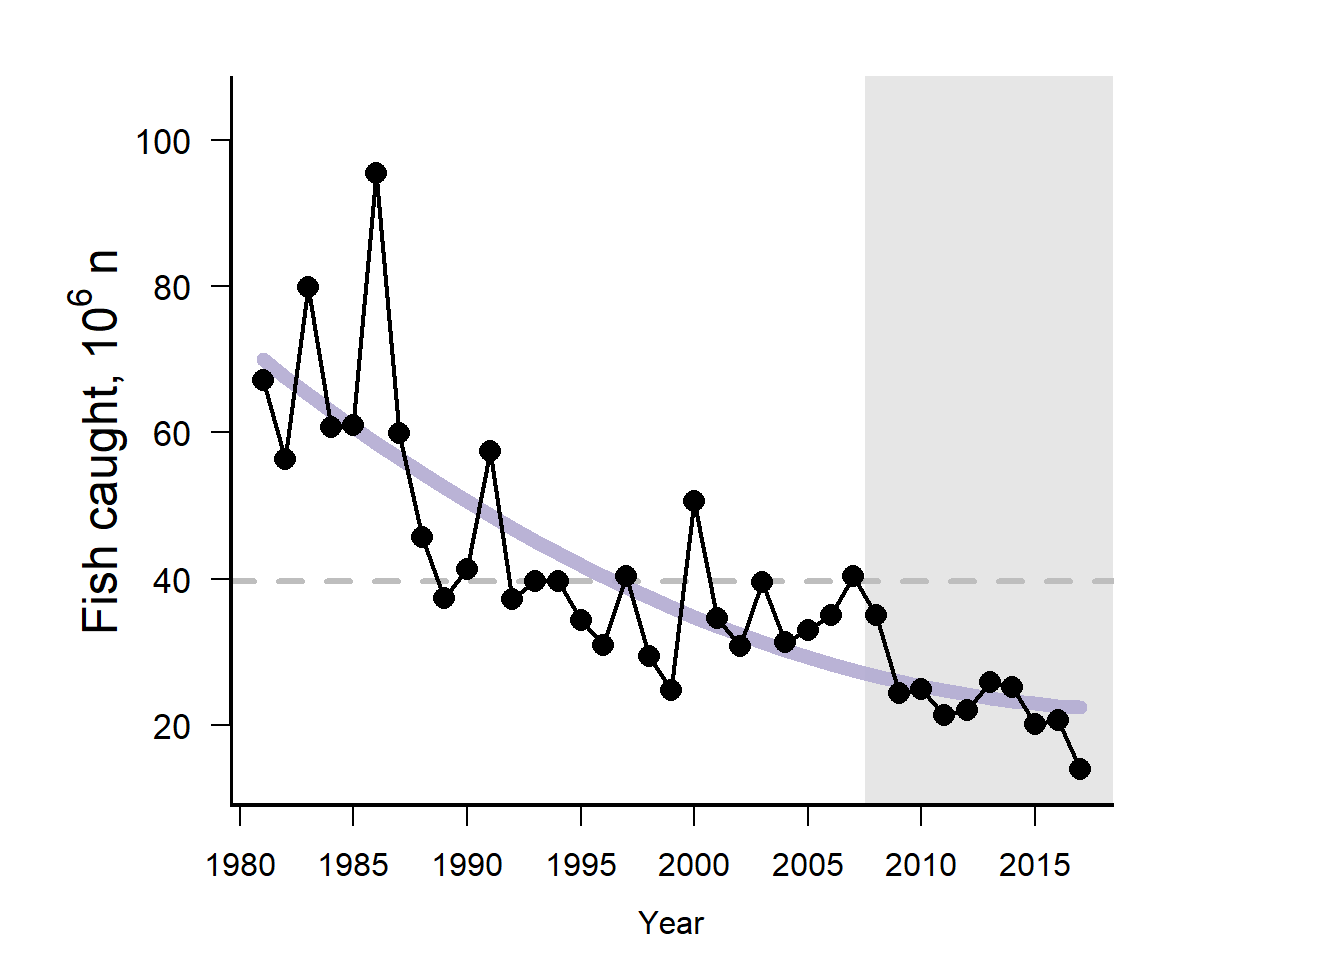
\includegraphics{C:/Users/kimberly.bastille/Desktop/tech-doc/imagesexamplefig-1.pdf}
\caption{\label{fig:examplefig}Example plot formatted for the report}
\end{figure}

\hypertarget{zooabund}{\chapter{Zooplankton}\label{zooabund}}

\textbf{Description}: Annual time series of zooplankton abundance

\textbf{Found in}: State of the Ecosystem - Gulf of Maine \& Georges
Bank (2017, 2018, 2019), State of the Ecosystem - Mid-Atlantic (2017,
2018, 2019)

\textbf{Indicator category}: Database pull with analysis; Synthesis of
published information; Extensive analysis, not yet published; Published
methods

\textbf{Contributor(s)}: Ryan Morse, Kevin Friedland

\textbf{Data steward}: Harvey Walsh,
\href{mailto:harvey.walsh@noaa.gov}{\nolinkurl{harvey.walsh@noaa.gov}};
Mike Jones,
\href{mailto:michael.jones@noaa.gov}{\nolinkurl{michael.jones@noaa.gov}}

\textbf{Point of contact}: Ryan Morse,
\href{mailto:ryan.morse@noaa.gov}{\nolinkurl{ryan.morse@noaa.gov}};
Harvey Walsh,
\href{mailto:harvey.walsh@noaa.gov}{\nolinkurl{harvey.walsh@noaa.gov}};
Kevin Friedland,
\href{mailto:kevin.friedland@noaa.gov}{\nolinkurl{kevin.friedland@noaa.gov}}

\textbf{Public availability statement}: Source data are publicly
available
\href{ftp://ftp.nefsc.noaa.gov/pub/hydro/zooplankton_data/}{here}.
Derived data can be found
\href{https://comet.nefsc.noaa.gov/erddap/tabledap/zoo_abundance_soe_v1.html}{here}.

\section{Methods}\label{methods-33}

\subsection{Data sources}\label{data-sources-33}

Zooplankton data are from the NOAA MARMAP and EcoMon cruises detailed
extensively in Kane (\protect\hyperlink{ref-Kane2007}{2007}), Kane
(\protect\hyperlink{ref-Kane2011}{2011}), and Morse et al.
(\protect\hyperlink{ref-Morse2017}{2017}).

\subsection{Data extraction}\label{data-extraction-25}

Data are from the publicly available zooplankton dataset on the NOAA FTP
server. The excel file has a list of excluded samples and cruises based
on Kane (\protect\hyperlink{ref-Kane2007}{2007}) and Kane
(\protect\hyperlink{ref-Kane2011}{2011}).

R code used in extraction process.

\begin{Shaded}
\begin{Highlighting}[]
\CommentTok{# load data}
\NormalTok{URL=}\StringTok{'ftp://ftp.nefsc.noaa.gov/pub/hydro/zooplankton_data/EcoMon_Plankton_Data_v3_0.xlsx'}
\NormalTok{ZPD=openxlsx}\OperatorTok{::}\KeywordTok{read.xlsx}\NormalTok{(URL, }\DataTypeTok{sheet=}\StringTok{'Data'}\NormalTok{)}
\end{Highlighting}
\end{Shaded}

\subsection{Data analysis}\label{data-analysis-31}

\textbf{Annual abundance anomalies}

Data are processed similarly to Kane
(\protect\hyperlink{ref-Kane2007}{2007}) and Perretti et al.
(\protect\hyperlink{ref-Perretti2017}{2017}\protect\hyperlink{ref-Perretti2017}{b}),
where a mean annual abundance by date is computed by area for each
species meeting inclusion metrics set in Morse et al.
(\protect\hyperlink{ref-Morse2017}{2017}). This is accomplished by
binning all samples for a given species to bi-monthly collection dates
based on median cruise date and taking the mean, then fitting a spline
interpolation between mean bi-monthly abundance to give expected
abundance on any given day of the year.

Abundance anomalies (Figure \ref{fig:zooplankton-abundance}) are
computed from the expected abundance on the day of sample collection.
Abundance anomaly time series are constructed for \emph{Centropages
typicus}, \emph{Pseudocalanus} spp., \emph{Calanus finmarchicus}, and
total zooplankton biovolume. The small-large copepod size index is
computed by averaging the individual abundance anomalies of
\emph{Pseudocalanus} spp., \emph{Centropages hamatus}, \emph{Centropages
typicus}, and \emph{Temora longicornis}, and subtracting the abundance
anomaly of \emph{Calanus finmarchicus}. This index tracks the overall
dominance of the small bodied copepods relative to the largest copepod
in the NEUS region, \emph{Calanus finmarchicus}.

\begin{Shaded}
\begin{Highlighting}[]
\CommentTok{#libraries}
\KeywordTok{library}\NormalTok{(vegan)}
\KeywordTok{library}\NormalTok{(stats)}
\KeywordTok{library}\NormalTok{(mgcv)}
\KeywordTok{library}\NormalTok{(reshape2)}
\KeywordTok{library}\NormalTok{(readxl)}
\KeywordTok{library}\NormalTok{(lubridate)}
\KeywordTok{library}\NormalTok{(sp)}
\KeywordTok{library}\NormalTok{(maptools)}
\KeywordTok{library}\NormalTok{(marmap)}
\KeywordTok{library}\NormalTok{(rgeos)}


\CommentTok{# load data}
\NormalTok{URL=}\StringTok{'ftp://ftp.nefsc.noaa.gov/pub/hydro/zooplankton_data/EcoMon_Plankton_Data_v3_0.xlsx'}
\NormalTok{ZPD=openxlsx}\OperatorTok{::}\KeywordTok{read.xlsx}\NormalTok{(URL, }\DataTypeTok{sheet=}\StringTok{'Data'}\NormalTok{)}
\CommentTok{# Fix date, time}
\NormalTok{dt=}\KeywordTok{as_date}\NormalTok{(ZPD}\OperatorTok{$}\NormalTok{date, }\DataTypeTok{origin =} \StringTok{"1899-12-30"}\NormalTok{)}
\NormalTok{DOY=}\KeywordTok{yday}\NormalTok{(dt) }\CommentTok{#day of year}
\NormalTok{month=}\KeywordTok{as.numeric}\NormalTok{(}\KeywordTok{format}\NormalTok{(dt, }\StringTok{'%m'}\NormalTok{))}
\NormalTok{year=}\KeywordTok{as.numeric}\NormalTok{(}\KeywordTok{format}\NormalTok{(dt, }\StringTok{'%Y'}\NormalTok{))}
\NormalTok{ZPD}\OperatorTok{$}\NormalTok{year=year}
\NormalTok{ZPD}\OperatorTok{$}\NormalTok{month=month}
\NormalTok{ZPD}\OperatorTok{$}\NormalTok{dt=dt}
\NormalTok{ZPD}\OperatorTok{$}\NormalTok{DOY=DOY}
\NormalTok{ZPD}\OperatorTok{$}\NormalTok{day=}\KeywordTok{as.numeric}\NormalTok{(}\KeywordTok{format}\NormalTok{(dt, }\StringTok{'%d'}\NormalTok{))}
\NormalTok{ZPD}\OperatorTok{$}\NormalTok{lat2=}\KeywordTok{ceiling}\NormalTok{(ZPD}\OperatorTok{$}\NormalTok{lat) }\CommentTok{#use for binning into 1 degree bins for removal of undersampled bins}
\NormalTok{ZPD}\OperatorTok{$}\NormalTok{lon2=}\KeywordTok{floor}\NormalTok{(ZPD}\OperatorTok{$}\NormalTok{lon) }\CommentTok{#use for binning into 1 degree bins for removal of undersampled bins}
\CommentTok{# ASSIGN EPU based on GPS data}
\NormalTok{## load shapefiles from EDAB EPU analysis ## not available here}

\NormalTok{gbk=}\KeywordTok{readShapeSpatial}\NormalTok{(}\StringTok{"EPU_GBKPoly.shp"}\NormalTok{)}
\NormalTok{gom=}\KeywordTok{readShapeSpatial}\NormalTok{(}\StringTok{"EPU_GOMPoly.shp"}\NormalTok{)}
\NormalTok{mab=}\KeywordTok{readShapeSpatial}\NormalTok{(}\StringTok{"EPU_MABPoly.shp"}\NormalTok{)}
\NormalTok{scs=}\KeywordTok{readShapeSpatial}\NormalTok{(}\StringTok{"EPU_SCSPoly.shp"}\NormalTok{)}
\CommentTok{#combine shapefiles GOM and GBK}
\NormalTok{gom.gbk.shp=}\KeywordTok{gUnion}\NormalTok{(gom, gbk, }\DataTypeTok{byid=}\NormalTok{F, }\DataTypeTok{id=}\OtherTok{NULL}\NormalTok{)}
\NormalTok{gom.gbk.shp=}\KeywordTok{gUnion}\NormalTok{(gom, gbk, }\DataTypeTok{byid=}\NormalTok{F, }\DataTypeTok{id=}\OtherTok{NULL}\NormalTok{)}
\NormalTok{gom.scs.shp=}\KeywordTok{gUnion}\NormalTok{(gom, scs, }\DataTypeTok{byid=}\NormalTok{F, }\DataTypeTok{id=}\OtherTok{NULL}\NormalTok{)}
\NormalTok{mab.gbk.shp=}\KeywordTok{gUnion}\NormalTok{(mab, gbk, }\DataTypeTok{byid=}\NormalTok{F, }\DataTypeTok{id=}\OtherTok{NULL}\NormalTok{)}
\NormalTok{NES.shp=}\KeywordTok{gUnion}\NormalTok{(mab.gbk.shp, gom.scs.shp, }\DataTypeTok{byid=}\NormalTok{F, }\DataTypeTok{id=}\OtherTok{NULL}\NormalTok{)}
\CommentTok{#extract just lat/lons for lines}
\NormalTok{gbk.lonlat =}\KeywordTok{as.data.frame}\NormalTok{(}\KeywordTok{lapply}\NormalTok{(}\KeywordTok{slot}\NormalTok{(gbk, }\StringTok{"polygons"}\NormalTok{), }\ControlFlowTok{function}\NormalTok{(x) }\KeywordTok{lapply}\NormalTok{(}\KeywordTok{slot}\NormalTok{(x, }\StringTok{"Polygons"}\NormalTok{), }\ControlFlowTok{function}\NormalTok{(y) }\KeywordTok{slot}\NormalTok{(y, }\StringTok{"coords"}\NormalTok{))))}
\NormalTok{gom.lonlat =}\KeywordTok{as.data.frame}\NormalTok{(}\KeywordTok{lapply}\NormalTok{(}\KeywordTok{slot}\NormalTok{(gom, }\StringTok{"polygons"}\NormalTok{), }\ControlFlowTok{function}\NormalTok{(x) }\KeywordTok{lapply}\NormalTok{(}\KeywordTok{slot}\NormalTok{(x, }\StringTok{"Polygons"}\NormalTok{), }\ControlFlowTok{function}\NormalTok{(y) }\KeywordTok{slot}\NormalTok{(y, }\StringTok{"coords"}\NormalTok{))))}
\NormalTok{mab.lonlat =}\KeywordTok{as.data.frame}\NormalTok{(}\KeywordTok{lapply}\NormalTok{(}\KeywordTok{slot}\NormalTok{(mab, }\StringTok{"polygons"}\NormalTok{), }\ControlFlowTok{function}\NormalTok{(x) }\KeywordTok{lapply}\NormalTok{(}\KeywordTok{slot}\NormalTok{(x, }\StringTok{"Polygons"}\NormalTok{), }\ControlFlowTok{function}\NormalTok{(y) }\KeywordTok{slot}\NormalTok{(y, }\StringTok{"coords"}\NormalTok{))))}
\NormalTok{scs.lonlat =}\KeywordTok{as.data.frame}\NormalTok{(}\KeywordTok{lapply}\NormalTok{(}\KeywordTok{slot}\NormalTok{(scs, }\StringTok{"polygons"}\NormalTok{), }\ControlFlowTok{function}\NormalTok{(x) }\KeywordTok{lapply}\NormalTok{(}\KeywordTok{slot}\NormalTok{(x, }\StringTok{"Polygons"}\NormalTok{), }\ControlFlowTok{function}\NormalTok{(y) }\KeywordTok{slot}\NormalTok{(y, }\StringTok{"coords"}\NormalTok{))))}
\NormalTok{gom.gbk.lonlat =}\KeywordTok{as.data.frame}\NormalTok{(}\KeywordTok{lapply}\NormalTok{(}\KeywordTok{slot}\NormalTok{(gom.gbk.shp, }\StringTok{"polygons"}\NormalTok{), }\ControlFlowTok{function}\NormalTok{(x) }\KeywordTok{lapply}\NormalTok{(}\KeywordTok{slot}\NormalTok{(x, }\StringTok{"Polygons"}\NormalTok{), }\ControlFlowTok{function}\NormalTok{(y) }\KeywordTok{slot}\NormalTok{(y, }\StringTok{"coords"}\NormalTok{))))}
\NormalTok{NES.lonlat =}\KeywordTok{as.data.frame}\NormalTok{(NES.shp}\OperatorTok{@}\NormalTok{polygons[[}\DecValTok{1}\NormalTok{]]}\OperatorTok{@}\NormalTok{Polygons[[}\DecValTok{1}\NormalTok{]]}\OperatorTok{@}\NormalTok{coords)}\CommentTok{# create matrix to use in in.out function}
\CommentTok{# create matrix to use in in.out function from package 'mgcv'}
\NormalTok{gom.mat=}\KeywordTok{as.matrix}\NormalTok{(gom.lonlat)}
\NormalTok{gbk.mat=}\KeywordTok{as.matrix}\NormalTok{(gbk.lonlat)}
\NormalTok{mab.mat=}\KeywordTok{as.matrix}\NormalTok{(mab.lonlat)}
\NormalTok{scs.mat=}\KeywordTok{as.matrix}\NormalTok{(scs.lonlat)}
\NormalTok{gom.gbk.mat=}\KeywordTok{as.matrix}\NormalTok{(gom.gbk.lonlat)}
\CommentTok{# assign samples to EPU}
\NormalTok{m4=}\KeywordTok{as.matrix}\NormalTok{(ZPD[,}\DecValTok{6}\OperatorTok{:}\DecValTok{5}\NormalTok{]) }\CommentTok{#lon,lat from ZPD}
\NormalTok{ZPD}\OperatorTok{$}\NormalTok{epu=}\OtherTok{NA}
\NormalTok{ZPD}\OperatorTok{$}\NormalTok{epu[}\KeywordTok{which}\NormalTok{(}\KeywordTok{in.out}\NormalTok{(gbk.mat, m4))]=}\StringTok{'GBK'}
\NormalTok{ZPD}\OperatorTok{$}\NormalTok{epu[}\KeywordTok{which}\NormalTok{(}\KeywordTok{in.out}\NormalTok{(gom.mat, m4))]=}\StringTok{'GOM'}
\NormalTok{ZPD}\OperatorTok{$}\NormalTok{epu[}\KeywordTok{which}\NormalTok{(}\KeywordTok{in.out}\NormalTok{(scs.mat, m4))]=}\StringTok{'SCS'}
\NormalTok{ZPD}\OperatorTok{$}\NormalTok{epu[}\KeywordTok{which}\NormalTok{(}\KeywordTok{in.out}\NormalTok{(mab.mat, m4))]=}\StringTok{'MAB'}
\NormalTok{test=ZPD[}\KeywordTok{is.na}\NormalTok{(ZPD}\OperatorTok{$}\NormalTok{epu),] }\CommentTok{#unassigned}
\NormalTok{nms=}\KeywordTok{data.frame}\NormalTok{(}\KeywordTok{colnames}\NormalTok{(ZPD)) }\CommentTok{# column names of orginal data}
\CommentTok{# limit data set to zooplankton from 1977 on}
\NormalTok{ZPDb=ZPD[,}\KeywordTok{c}\NormalTok{(}\KeywordTok{seq}\NormalTok{(}\DecValTok{1}\NormalTok{,}\DecValTok{14}\NormalTok{,}\DecValTok{1}\NormalTok{), }\KeywordTok{seq}\NormalTok{(}\DecValTok{290}\NormalTok{,}\DecValTok{297}\NormalTok{,}\DecValTok{1}\NormalTok{), }\KeywordTok{seq}\NormalTok{(}\DecValTok{106}\NormalTok{,}\DecValTok{197}\NormalTok{,}\DecValTok{1}\NormalTok{))] }\CommentTok{# check to make sure these are correct against 'nms' if data source changes!!!}
\NormalTok{ZPDb=ZPDb[}\KeywordTok{order}\NormalTok{(ZPDb}\OperatorTok{$}\NormalTok{date),]}
\NormalTok{ZPDb=ZPDb[}\KeywordTok{which}\NormalTok{(ZPDb}\OperatorTok{$}\NormalTok{year }\OperatorTok{>}\StringTok{ }\DecValTok{1976}\NormalTok{),] }\CommentTok{# remove NA data in years prior to 1977}
\CommentTok{# Select only taxa present in yearly data > x percent of samples}
\NormalTok{X=}\DecValTok{20} \CommentTok{# percent criteria to use as minimum percent in samples}
\NormalTok{ZPDa=ZPDb}
\NormalTok{ZPDa=ZPDa[}\OperatorTok{!}\KeywordTok{is.na}\NormalTok{(ZPDa}\OperatorTok{$}\NormalTok{zoo_gear),] }\CommentTok{# Remove NA in zooplankton rows}
\CommentTok{# Reduce to taxa occurrance > x percent in samples}
\NormalTok{p.a=ZPDa[,}\DecValTok{24}\OperatorTok{:}\DecValTok{114}\NormalTok{]}
\NormalTok{p.a[p.a }\OperatorTok{>}\StringTok{ }\DecValTok{0}\NormalTok{]=}\DecValTok{1} \CommentTok{# presence/absence}
\NormalTok{count=}\KeywordTok{colSums}\NormalTok{(p.a)}
\NormalTok{pct=(count}\OperatorTok{/}\KeywordTok{dim}\NormalTok{(ZPDa)[}\DecValTok{1}\NormalTok{])}\OperatorTok{*}\DecValTok{100}
\NormalTok{crit=}\KeywordTok{which}\NormalTok{(pct}\OperatorTok{>}\NormalTok{X)}
\NormalTok{ZPDa=ZPDa[}\KeywordTok{c}\NormalTok{(}\DecValTok{1}\OperatorTok{:}\DecValTok{23}\NormalTok{,crit}\OperatorTok{+}\DecValTok{23}\NormalTok{)] }\CommentTok{# data limited to taxa occurring in > X percent of samples}

\CommentTok{#Take median date from each cruise and assign cruise to bimonth for bi-monthly means aggregation}
\NormalTok{cruises=}\KeywordTok{unique}\NormalTok{(ZPDa}\OperatorTok{$}\NormalTok{cruise_name)}
\ControlFlowTok{for}\NormalTok{ (i }\ControlFlowTok{in} \DecValTok{1}\OperatorTok{:}\KeywordTok{length}\NormalTok{(cruises))\{}
\NormalTok{  ZPDa}\OperatorTok{$}\NormalTok{medmonth[ZPDa}\OperatorTok{$}\NormalTok{cruise_name }\OperatorTok{==}\StringTok{ }\NormalTok{cruises[i]]=}\KeywordTok{median}\NormalTok{(ZPDa}\OperatorTok{$}\NormalTok{DOY[ZPDa}\OperatorTok{$}\NormalTok{cruise_name }\OperatorTok{==}\StringTok{ }\NormalTok{cruises[i]])}
\NormalTok{\}}
\NormalTok{ZPDa}\OperatorTok{$}\NormalTok{bmm=}\OtherTok{NA}
\NormalTok{ZPDa}\OperatorTok{$}\NormalTok{bmm[}\KeywordTok{which}\NormalTok{(}\KeywordTok{as.integer}\NormalTok{(ZPDa}\OperatorTok{$}\NormalTok{medmonth) }\OperatorTok\StringTok{ }\KeywordTok{seq}\NormalTok{(}\DecValTok{0}\NormalTok{,}\DecValTok{59}\NormalTok{))]=}\DecValTok{1}
\NormalTok{ZPDa}\OperatorTok{$}\NormalTok{bmm[}\KeywordTok{which}\NormalTok{(}\KeywordTok{as.integer}\NormalTok{(ZPDa}\OperatorTok{$}\NormalTok{medmonth) }\OperatorTok\StringTok{ }\KeywordTok{seq}\NormalTok{(}\DecValTok{60}\NormalTok{,}\DecValTok{120}\NormalTok{))]=}\DecValTok{3}
\NormalTok{ZPDa}\OperatorTok{$}\NormalTok{bmm[}\KeywordTok{which}\NormalTok{(}\KeywordTok{as.integer}\NormalTok{(ZPDa}\OperatorTok{$}\NormalTok{medmonth) }\OperatorTok\StringTok{ }\KeywordTok{seq}\NormalTok{(}\DecValTok{121}\NormalTok{,}\DecValTok{181}\NormalTok{))]=}\DecValTok{5}
\NormalTok{ZPDa}\OperatorTok{$}\NormalTok{bmm[}\KeywordTok{which}\NormalTok{(}\KeywordTok{as.integer}\NormalTok{(ZPDa}\OperatorTok{$}\NormalTok{medmonth) }\OperatorTok\StringTok{ }\KeywordTok{seq}\NormalTok{(}\DecValTok{182}\NormalTok{,}\DecValTok{243}\NormalTok{))]=}\DecValTok{7}
\NormalTok{ZPDa}\OperatorTok{$}\NormalTok{bmm[}\KeywordTok{which}\NormalTok{(}\KeywordTok{as.integer}\NormalTok{(ZPDa}\OperatorTok{$}\NormalTok{medmonth) }\OperatorTok\StringTok{ }\KeywordTok{seq}\NormalTok{(}\DecValTok{244}\NormalTok{,}\DecValTok{304}\NormalTok{))]=}\DecValTok{9}
\NormalTok{ZPDa}\OperatorTok{$}\NormalTok{bmm[}\KeywordTok{which}\NormalTok{(}\KeywordTok{as.integer}\NormalTok{(ZPDa}\OperatorTok{$}\NormalTok{medmonth) }\OperatorTok\StringTok{ }\KeywordTok{seq}\NormalTok{(}\DecValTok{305}\NormalTok{,}\DecValTok{366}\NormalTok{))]=}\DecValTok{11}

\NormalTok{ZPDa[,}\DecValTok{14}\NormalTok{]=}\KeywordTok{as.numeric}\NormalTok{(ZPDa[,}\DecValTok{14}\NormalTok{])}
\NormalTok{ZPDa[,}\DecValTok{23}\NormalTok{]=}\KeywordTok{as.numeric}\NormalTok{(ZPDa[,}\DecValTok{23}\NormalTok{])}
\NormalTok{ZPDsave=ZPDa }\CommentTok{#from above routine, Yearly (all data) }

\NormalTok{SEASON=}\StringTok{'Yearly'}
\NormalTok{ZPDa=ZPDsave}
\CommentTok{# LOG transform data using ZPDa from above (select season first)}
\NormalTok{test=}\KeywordTok{log10}\NormalTok{(ZPDa[,}\DecValTok{24}\OperatorTok{:}\DecValTok{50}\NormalTok{]}\OperatorTok{+}\DecValTok{1}\NormalTok{) }\CommentTok{#choose columns with zooplankton data}
\NormalTok{ZPDlog=ZPDa}
\NormalTok{ZPDlog[,}\DecValTok{24}\OperatorTok{:}\DecValTok{50}\NormalTok{]=test}
\NormalTok{nm=}\KeywordTok{matrix}\NormalTok{(}\KeywordTok{colnames}\NormalTok{(ZPDlog))}

\NormalTok{area=}\StringTok{'GBK'}
\NormalTok{gbk.yr.spln=}\KeywordTok{data.frame}\NormalTok{()}
\ControlFlowTok{for}\NormalTok{ (i }\ControlFlowTok{in} \DecValTok{23}\OperatorTok{:}\DecValTok{50}\NormalTok{)\{}
\NormalTok{  num=i}
\NormalTok{  name=nm[num,}\DecValTok{1}\NormalTok{]}
\NormalTok{  mean.loc.x=}\KeywordTok{aggregate}\NormalTok{(ZPDlog[}\KeywordTok{which}\NormalTok{(ZPDlog}\OperatorTok{$}\NormalTok{epu}\OperatorTok{==}\NormalTok{area),num], }\DataTypeTok{by=}\KeywordTok{list}\NormalTok{(ZPDlog}\OperatorTok{$}\NormalTok{bmm[}\KeywordTok{which}\NormalTok{(ZPDlog}\OperatorTok{$}\NormalTok{epu}\OperatorTok{==}\NormalTok{area)]), }\DataTypeTok{FUN=}\NormalTok{mean, }\DataTypeTok{na.rm=}\NormalTok{T)}
\NormalTok{  func =}\StringTok{ }\KeywordTok{splinefun}\NormalTok{(mean.loc.x[,}\DecValTok{1}\NormalTok{], }\DataTypeTok{y=}\NormalTok{mean.loc.x[,}\DecValTok{2}\NormalTok{], }\DataTypeTok{method=}\StringTok{"natural"}\NormalTok{,  }\DataTypeTok{ties =}\NormalTok{ mean)  }
\NormalTok{  x.daily=}\KeywordTok{func}\NormalTok{(}\KeywordTok{seq}\NormalTok{(}\DecValTok{1}\NormalTok{, }\DecValTok{12}\NormalTok{, }\FloatTok{0.0302}\NormalTok{)) }\CommentTok{#365 days}
\NormalTok{  gbk.yr.spln=}\KeywordTok{rbind}\NormalTok{(gbk.yr.spln,x.daily)}
\NormalTok{\}}
\NormalTok{gbk.yr.spln=}\KeywordTok{t}\NormalTok{(gbk.yr.spln)}
\KeywordTok{rownames}\NormalTok{(gbk.yr.spln)=}\KeywordTok{seq}\NormalTok{(}\DecValTok{1}\OperatorTok{:}\DecValTok{365}\NormalTok{); }\KeywordTok{colnames}\NormalTok{(gbk.yr.spln)=nm[}\DecValTok{23}\OperatorTok{:}\DecValTok{50}\NormalTok{,}\DecValTok{1}\NormalTok{]}

\NormalTok{area=}\StringTok{'GOM'}
\NormalTok{gom.yr.spln=}\KeywordTok{data.frame}\NormalTok{()}
\ControlFlowTok{for}\NormalTok{ (i }\ControlFlowTok{in} \DecValTok{23}\OperatorTok{:}\DecValTok{50}\NormalTok{)\{}
\NormalTok{  num=i}
\NormalTok{  name=nm[num,}\DecValTok{1}\NormalTok{]}
\NormalTok{  mean.loc.x=}\KeywordTok{aggregate}\NormalTok{(ZPDlog[}\KeywordTok{which}\NormalTok{(ZPDlog}\OperatorTok{$}\NormalTok{epu}\OperatorTok{==}\NormalTok{area),num], }\DataTypeTok{by=}\KeywordTok{list}\NormalTok{(ZPDlog}\OperatorTok{$}\NormalTok{bmm[}\KeywordTok{which}\NormalTok{(ZPDlog}\OperatorTok{$}\NormalTok{epu}\OperatorTok{==}\NormalTok{area)]), }\DataTypeTok{FUN=}\NormalTok{mean, }\DataTypeTok{na.rm=}\NormalTok{T)}
\NormalTok{  func =}\StringTok{ }\KeywordTok{splinefun}\NormalTok{(mean.loc.x[,}\DecValTok{1}\NormalTok{], }\DataTypeTok{y=}\NormalTok{mean.loc.x[,}\DecValTok{2}\NormalTok{], }\DataTypeTok{method=}\StringTok{"natural"}\NormalTok{,  }\DataTypeTok{ties =}\NormalTok{ mean)}
\NormalTok{  x.daily=}\KeywordTok{func}\NormalTok{(}\KeywordTok{seq}\NormalTok{(}\DecValTok{1}\NormalTok{, }\DecValTok{12}\NormalTok{, }\FloatTok{0.0302}\NormalTok{)) }\CommentTok{#365 days}
\NormalTok{  gom.yr.spln=}\KeywordTok{rbind}\NormalTok{(gom.yr.spln,x.daily)}
\NormalTok{\}}
\NormalTok{gom.yr.spln=}\KeywordTok{t}\NormalTok{(gom.yr.spln)}
\KeywordTok{rownames}\NormalTok{(gom.yr.spln)=}\KeywordTok{seq}\NormalTok{(}\DecValTok{1}\OperatorTok{:}\DecValTok{365}\NormalTok{); }\KeywordTok{colnames}\NormalTok{(gom.yr.spln)=nm[}\DecValTok{23}\OperatorTok{:}\DecValTok{50}\NormalTok{,}\DecValTok{1}\NormalTok{]}

\NormalTok{area=}\StringTok{'MAB'}
\NormalTok{mab.yr.spln=}\KeywordTok{data.frame}\NormalTok{()}
\ControlFlowTok{for}\NormalTok{ (i }\ControlFlowTok{in} \DecValTok{23}\OperatorTok{:}\DecValTok{50}\NormalTok{)\{}
\NormalTok{  num=i}
\NormalTok{  name=nm[num,}\DecValTok{1}\NormalTok{]}
\NormalTok{  mean.loc.x=}\KeywordTok{aggregate}\NormalTok{(ZPDlog[}\KeywordTok{which}\NormalTok{(ZPDlog}\OperatorTok{$}\NormalTok{epu}\OperatorTok{==}\NormalTok{area),num], }\DataTypeTok{by=}\KeywordTok{list}\NormalTok{(ZPDlog}\OperatorTok{$}\NormalTok{bmm[}\KeywordTok{which}\NormalTok{(ZPDlog}\OperatorTok{$}\NormalTok{epu}\OperatorTok{==}\NormalTok{area)]), }\DataTypeTok{FUN=}\NormalTok{mean, }\DataTypeTok{na.rm=}\NormalTok{T)}
\NormalTok{  func =}\StringTok{ }\KeywordTok{splinefun}\NormalTok{(mean.loc.x[,}\DecValTok{1}\NormalTok{], }\DataTypeTok{y=}\NormalTok{mean.loc.x[,}\DecValTok{2}\NormalTok{], }\DataTypeTok{method=}\StringTok{"natural"}\NormalTok{,  }\DataTypeTok{ties =}\NormalTok{ mean)}
\NormalTok{  x.daily=}\KeywordTok{func}\NormalTok{(}\KeywordTok{seq}\NormalTok{(}\DecValTok{1}\NormalTok{, }\DecValTok{12}\NormalTok{, }\FloatTok{0.0302}\NormalTok{)) }\CommentTok{#365 days}
\NormalTok{  mab.yr.spln=}\KeywordTok{rbind}\NormalTok{(mab.yr.spln,x.daily)}
\NormalTok{\}}
\NormalTok{mab.yr.spln=}\KeywordTok{t}\NormalTok{(mab.yr.spln)}
\KeywordTok{rownames}\NormalTok{(mab.yr.spln)=}\KeywordTok{seq}\NormalTok{(}\DecValTok{1}\OperatorTok{:}\DecValTok{365}\NormalTok{); }\KeywordTok{colnames}\NormalTok{(mab.yr.spln)=nm[}\DecValTok{23}\OperatorTok{:}\DecValTok{50}\NormalTok{,}\DecValTok{1}\NormalTok{]}

\NormalTok{area=}\StringTok{'SCS'}
\NormalTok{scs.yr.spln=}\KeywordTok{data.frame}\NormalTok{()}
\ControlFlowTok{for}\NormalTok{ (i }\ControlFlowTok{in} \DecValTok{23}\OperatorTok{:}\DecValTok{50}\NormalTok{)\{}
\NormalTok{  num=i}
\NormalTok{  name=nm[num,}\DecValTok{1}\NormalTok{]}
\NormalTok{  mean.loc.x=}\KeywordTok{aggregate}\NormalTok{(ZPDlog[}\KeywordTok{which}\NormalTok{(ZPDlog}\OperatorTok{$}\NormalTok{epu}\OperatorTok{==}\NormalTok{area),num], }\DataTypeTok{by=}\KeywordTok{list}\NormalTok{(ZPDlog}\OperatorTok{$}\NormalTok{bmm[}\KeywordTok{which}\NormalTok{(ZPDlog}\OperatorTok{$}\NormalTok{epu}\OperatorTok{==}\NormalTok{area)]), }\DataTypeTok{FUN=}\NormalTok{mean, }\DataTypeTok{na.rm=}\NormalTok{T)}
\NormalTok{  func =}\StringTok{ }\KeywordTok{splinefun}\NormalTok{(mean.loc.x[,}\DecValTok{1}\NormalTok{], }\DataTypeTok{y=}\NormalTok{mean.loc.x[,}\DecValTok{2}\NormalTok{], }\DataTypeTok{method=}\StringTok{"natural"}\NormalTok{,  }\DataTypeTok{ties =}\NormalTok{ mean)}
\NormalTok{  x.daily=}\KeywordTok{func}\NormalTok{(}\KeywordTok{seq}\NormalTok{(}\DecValTok{1}\NormalTok{, }\DecValTok{12}\NormalTok{, }\FloatTok{0.0302}\NormalTok{)) }\CommentTok{#365 days}
\NormalTok{  scs.yr.spln=}\KeywordTok{rbind}\NormalTok{(scs.yr.spln,x.daily)}
\NormalTok{\}}
\NormalTok{scs.yr.spln=}\KeywordTok{t}\NormalTok{(scs.yr.spln)}
\KeywordTok{rownames}\NormalTok{(scs.yr.spln)=}\KeywordTok{seq}\NormalTok{(}\DecValTok{1}\OperatorTok{:}\DecValTok{365}\NormalTok{); }\KeywordTok{colnames}\NormalTok{(scs.yr.spln)=nm[}\DecValTok{23}\OperatorTok{:}\DecValTok{50}\NormalTok{,}\DecValTok{1}\NormalTok{]}

\CommentTok{# Subtract mean expected value from observed abundance to get anomaly}
\NormalTok{gbk.anom=ZPDlog[}\KeywordTok{which}\NormalTok{(ZPDlog}\OperatorTok{$}\NormalTok{epu}\OperatorTok{==}\StringTok{'GBK'}\NormalTok{),]}
\NormalTok{gom.anom=ZPDlog[}\KeywordTok{which}\NormalTok{(ZPDlog}\OperatorTok{$}\NormalTok{epu}\OperatorTok{==}\StringTok{'GOM'}\NormalTok{),]}
\NormalTok{mab.anom=ZPDlog[}\KeywordTok{which}\NormalTok{(ZPDlog}\OperatorTok{$}\NormalTok{epu}\OperatorTok{==}\StringTok{'MAB'}\NormalTok{),]}
\NormalTok{scs.anom=ZPDlog[}\KeywordTok{which}\NormalTok{(ZPDlog}\OperatorTok{$}\NormalTok{epu}\OperatorTok{==}\StringTok{'SCS'}\NormalTok{),]}

\NormalTok{gbk.anom.b=}\KeywordTok{data.frame}\NormalTok{(}\KeywordTok{matrix}\NormalTok{(}\OtherTok{NA}\NormalTok{, }\DataTypeTok{nrow =} \KeywordTok{dim}\NormalTok{(gbk.anom)[}\DecValTok{1}\NormalTok{], }\DataTypeTok{ncol =} \KeywordTok{dim}\NormalTok{(gbk.anom)[}\DecValTok{2}\NormalTok{]))}
\ControlFlowTok{for}\NormalTok{ (i }\ControlFlowTok{in} \DecValTok{1}\OperatorTok{:}\KeywordTok{dim}\NormalTok{(gbk.anom)[}\DecValTok{1}\NormalTok{])\{}
\NormalTok{  gbk.anom.b[i,}\DecValTok{23}\OperatorTok{:}\DecValTok{50}\NormalTok{]=gbk.anom[i,}\DecValTok{23}\OperatorTok{:}\DecValTok{50}\NormalTok{]}\OperatorTok{-}\NormalTok{gbk.yr.spln[}\KeywordTok{which}\NormalTok{(gbk.anom}\OperatorTok{$}\NormalTok{DOY[i]}\OperatorTok{==}\KeywordTok{rownames}\NormalTok{(gbk.yr.spln)),]}
\NormalTok{\}}
\NormalTok{gom.anom.b=}\KeywordTok{data.frame}\NormalTok{(}\KeywordTok{matrix}\NormalTok{(}\OtherTok{NA}\NormalTok{, }\DataTypeTok{nrow =} \KeywordTok{dim}\NormalTok{(gom.anom)[}\DecValTok{1}\NormalTok{], }\DataTypeTok{ncol =} \KeywordTok{dim}\NormalTok{(gom.anom)[}\DecValTok{2}\NormalTok{]))}
\ControlFlowTok{for}\NormalTok{ (i }\ControlFlowTok{in} \DecValTok{1}\OperatorTok{:}\KeywordTok{dim}\NormalTok{(gom.anom)[}\DecValTok{1}\NormalTok{])\{}
\NormalTok{  gom.anom.b[i,}\DecValTok{23}\OperatorTok{:}\DecValTok{50}\NormalTok{]=gom.anom[i,}\DecValTok{23}\OperatorTok{:}\DecValTok{50}\NormalTok{]}\OperatorTok{-}\NormalTok{gom.yr.spln[}\KeywordTok{which}\NormalTok{(gom.anom}\OperatorTok{$}\NormalTok{DOY[i]}\OperatorTok{==}\KeywordTok{rownames}\NormalTok{(gom.yr.spln)),]}
\NormalTok{\}}
\NormalTok{mab.anom.b=}\KeywordTok{data.frame}\NormalTok{(}\KeywordTok{matrix}\NormalTok{(}\OtherTok{NA}\NormalTok{, }\DataTypeTok{nrow =} \KeywordTok{dim}\NormalTok{(mab.anom)[}\DecValTok{1}\NormalTok{], }\DataTypeTok{ncol =} \KeywordTok{dim}\NormalTok{(mab.anom)[}\DecValTok{2}\NormalTok{]))}
\ControlFlowTok{for}\NormalTok{ (i }\ControlFlowTok{in} \DecValTok{1}\OperatorTok{:}\KeywordTok{dim}\NormalTok{(mab.anom)[}\DecValTok{1}\NormalTok{])\{}
\NormalTok{  mab.anom.b[i,}\DecValTok{23}\OperatorTok{:}\DecValTok{50}\NormalTok{]=mab.anom[i,}\DecValTok{23}\OperatorTok{:}\DecValTok{50}\NormalTok{]}\OperatorTok{-}\NormalTok{mab.yr.spln[}\KeywordTok{which}\NormalTok{(mab.anom}\OperatorTok{$}\NormalTok{DOY[i]}\OperatorTok{==}\KeywordTok{rownames}\NormalTok{(mab.yr.spln)),]}
\NormalTok{\}}
\NormalTok{scs.anom.b=}\KeywordTok{data.frame}\NormalTok{(}\KeywordTok{matrix}\NormalTok{(}\OtherTok{NA}\NormalTok{, }\DataTypeTok{nrow =} \KeywordTok{dim}\NormalTok{(scs.anom)[}\DecValTok{1}\NormalTok{], }\DataTypeTok{ncol =} \KeywordTok{dim}\NormalTok{(scs.anom)[}\DecValTok{2}\NormalTok{]))}
\ControlFlowTok{for}\NormalTok{ (i }\ControlFlowTok{in} \DecValTok{1}\OperatorTok{:}\KeywordTok{dim}\NormalTok{(scs.anom)[}\DecValTok{1}\NormalTok{])\{}
\NormalTok{  scs.anom.b[i,}\DecValTok{23}\OperatorTok{:}\DecValTok{50}\NormalTok{]=scs.anom[i,}\DecValTok{23}\OperatorTok{:}\DecValTok{50}\NormalTok{]}\OperatorTok{-}\NormalTok{scs.yr.spln[}\KeywordTok{which}\NormalTok{(scs.anom}\OperatorTok{$}\NormalTok{DOY[i]}\OperatorTok{==}\KeywordTok{rownames}\NormalTok{(scs.yr.spln)),]}
\NormalTok{\}  }

\NormalTok{scs.anom.b=}\KeywordTok{rbind}\NormalTok{(scs.anom.b,test)}
\CommentTok{# Aggregrate by Year, Yearly anomaly by epu}
\NormalTok{gbk.yr.anom=}\KeywordTok{aggregate}\NormalTok{(gbk.anom.b, }\DataTypeTok{by=}\KeywordTok{list}\NormalTok{(gbk.anom}\OperatorTok{$}\NormalTok{year), }\DataTypeTok{FUN=}\NormalTok{mean, }\DataTypeTok{na.rm=}\NormalTok{T); }\KeywordTok{rownames}\NormalTok{(gbk.yr.anom)=gbk.yr.anom[,}\DecValTok{1}\NormalTok{]; gbk.yr.anom[,}\DecValTok{1}\NormalTok{]=}\OtherTok{NULL}\NormalTok{; }\KeywordTok{colnames}\NormalTok{(gbk.yr.anom)=}\KeywordTok{colnames}\NormalTok{(gbk.anom)}
\NormalTok{gom.yr.anom=}\KeywordTok{aggregate}\NormalTok{(gom.anom.b, }\DataTypeTok{by=}\KeywordTok{list}\NormalTok{(gom.anom}\OperatorTok{$}\NormalTok{year), }\DataTypeTok{FUN=}\NormalTok{mean, }\DataTypeTok{na.rm=}\NormalTok{T); }\KeywordTok{rownames}\NormalTok{(gom.yr.anom)=gom.yr.anom[,}\DecValTok{1}\NormalTok{]; gom.yr.anom[,}\DecValTok{1}\NormalTok{]=}\OtherTok{NULL}\NormalTok{; }\KeywordTok{colnames}\NormalTok{(gom.yr.anom)=}\KeywordTok{colnames}\NormalTok{(gom.anom)}
\NormalTok{mab.yr.anom=}\KeywordTok{aggregate}\NormalTok{(mab.anom.b, }\DataTypeTok{by=}\KeywordTok{list}\NormalTok{(mab.anom}\OperatorTok{$}\NormalTok{year), }\DataTypeTok{FUN=}\NormalTok{mean, }\DataTypeTok{na.rm=}\NormalTok{T); }\KeywordTok{rownames}\NormalTok{(mab.yr.anom)=mab.yr.anom[,}\DecValTok{1}\NormalTok{]; mab.yr.anom[,}\DecValTok{1}\NormalTok{]=}\OtherTok{NULL}\NormalTok{; }\KeywordTok{colnames}\NormalTok{(mab.yr.anom)=}\KeywordTok{colnames}\NormalTok{(mab.anom)}
\NormalTok{scs.yr.anom=}\KeywordTok{aggregate}\NormalTok{(scs.anom.b, }\DataTypeTok{by=}\KeywordTok{list}\NormalTok{(scs.anom}\OperatorTok{$}\NormalTok{year), }\DataTypeTok{FUN=}\NormalTok{mean, }\DataTypeTok{na.rm=}\NormalTok{T); }\KeywordTok{rownames}\NormalTok{(scs.yr.anom)=scs.yr.anom[,}\DecValTok{1}\NormalTok{]; scs.yr.anom[,}\DecValTok{1}\NormalTok{]=}\OtherTok{NULL}\NormalTok{; }\KeywordTok{colnames}\NormalTok{(scs.yr.anom)=}\KeywordTok{colnames}\NormalTok{(scs.anom)}

\CommentTok{# Small-Large body copepod abundance anomaly}
\NormalTok{lgtx=}\KeywordTok{c}\NormalTok{(}\DecValTok{25}\NormalTok{) }\CommentTok{#column for Calanus finmarchicus}
\NormalTok{smtx=}\KeywordTok{c}\NormalTok{(}\DecValTok{26}\NormalTok{,}\DecValTok{24}\NormalTok{,}\DecValTok{28}\NormalTok{,}\DecValTok{27}\NormalTok{) }\CommentTok{#Pseudocalanus spp, Centropoges typicus, Centropages hamatus, Temora longicornis}

\NormalTok{dataTsm=gbk.yr.anom[,smtx]}
\NormalTok{dataTlg=gbk.yr.anom[,lgtx]}
\NormalTok{anom.gbk=}\KeywordTok{rowMeans}\NormalTok{(dataTsm)}\OperatorTok{-}\NormalTok{(dataTlg)}
\NormalTok{dataTsm=gom.yr.anom[,smtx]}
\NormalTok{dataTlg=gom.yr.anom[,lgtx]}
\NormalTok{anom.gom=}\KeywordTok{rowMeans}\NormalTok{(dataTsm)}\OperatorTok{-}\NormalTok{(dataTlg)}
\NormalTok{dataTsm=mab.yr.anom[,smtx]}
\NormalTok{dataTlg=mab.yr.anom[,lgtx]}
\NormalTok{anom.mab=}\KeywordTok{rowMeans}\NormalTok{(dataTsm)}\OperatorTok{-}\NormalTok{(dataTlg)}
\NormalTok{dataTsm=scs.yr.anom[,smtx]}
\NormalTok{dataTlg=scs.yr.anom[,lgtx]}
\NormalTok{anom.scs=}\KeywordTok{rowMeans}\NormalTok{(dataTsm)}\OperatorTok{-}\NormalTok{(dataTlg)}
\end{Highlighting}
\end{Shaded}

\textbf{Seasonal abundance}

Time series of zooplankton abundance in the spring and fall months have
been presented in the 2019 Mid-Atlantic State of the Ecosystem report.
Raw abundance data were sourced from the EcoMon cruises referenced
above, and ordinary kriging was used to estimate seasonal abundance over
the Northeast Shelf. These data were then aggregated further into time
series of mean abundance by Ecological Production Unit. These data are
presented in Figure \ref{fig:MAB-oi-zoo}.

\subsection{Data processing}\label{data-processing-19}

Zooplankton abundances indicators were formatted for inclusion in the
ecodata R package using the following code.

\textbf{Abundance anomaly}

\begin{Shaded}
\begin{Highlighting}[]
\CommentTok{# Process zooplankton abundance anomalies and small-large index }

\KeywordTok{library}\NormalTok{(dplyr)}
\KeywordTok{library}\NormalTok{(tidyr)}

\NormalTok{raw.dir <-}\StringTok{ }\NormalTok{here}\OperatorTok{::}\KeywordTok{here}\NormalTok{(}\StringTok{"data-raw"}\NormalTok{)}

\NormalTok{get_zoo_anom_sli <-}\StringTok{ }\ControlFlowTok{function}\NormalTok{(}\DataTypeTok{save_clean =}\NormalTok{ F)\{}
  
  \KeywordTok{load}\NormalTok{(}\KeywordTok{file.path}\NormalTok{(raw.dir, }\StringTok{"1977_2017_SLI_Calfin_Pseudo_Ctyp.Rdata"}\NormalTok{))}
  
\NormalTok{  zoo_anom_sli <-}\StringTok{ }\NormalTok{Zooplankton_Primary_Prod }\OperatorTok
\StringTok{  }\KeywordTok{gather}\NormalTok{(.,Var, Value, }\OperatorTok{-}\NormalTok{year) }\OperatorTok\StringTok{ }
\StringTok{  }\NormalTok{dplyr}\OperatorTok{::}\KeywordTok{rename}\NormalTok{(}\DataTypeTok{Time =}\NormalTok{ year) }\OperatorTok\StringTok{ }
\StringTok{  }\KeywordTok{separate}\NormalTok{(., Var, }\KeywordTok{c}\NormalTok{(}\StringTok{"Var"}\NormalTok{,}\StringTok{"EPU"}\NormalTok{)) }\OperatorTok\StringTok{ }
\StringTok{  }\KeywordTok{mutate}\NormalTok{(}\DataTypeTok{EPU =}\NormalTok{ plyr}\OperatorTok{::}\KeywordTok{mapvalues}\NormalTok{(EPU, }\DataTypeTok{from =} \KeywordTok{c}\NormalTok{(}\StringTok{"gom"}\NormalTok{,}\StringTok{"gbk"}\NormalTok{,}\StringTok{"scs"}\NormalTok{,}\StringTok{"mab"}\NormalTok{), }
                               \DataTypeTok{to =} \KeywordTok{c}\NormalTok{(}\StringTok{"GOM"}\NormalTok{,}\StringTok{"GB"}\NormalTok{,}\StringTok{"SS"}\NormalTok{,}\StringTok{"MAB"}\NormalTok{)),}
         \DataTypeTok{Var =}\NormalTok{ plyr}\OperatorTok{::}\KeywordTok{mapvalues}\NormalTok{(Var, }\DataTypeTok{from =} \KeywordTok{c}\NormalTok{(}\StringTok{"PseAnom"}\NormalTok{,}
                                             \StringTok{"CtyAnom"}\NormalTok{,}
                                             \StringTok{"CalAnom"}\NormalTok{,}
                                             \StringTok{"SLI"}\NormalTok{), }
                               \DataTypeTok{to =} \KeywordTok{c}\NormalTok{(}\StringTok{"pseudocalanus anomaly"}\NormalTok{,}
                                      \StringTok{"centropages anomaly"}\NormalTok{,}
                                      \StringTok{"calanus anomaly"}\NormalTok{,}
                                      \StringTok{"small-large index"}\NormalTok{)),}
         \DataTypeTok{Units =} \StringTok{"anomaly"}\NormalTok{)}
  
  \ControlFlowTok{if}\NormalTok{ (save_clean)\{}
\NormalTok{    usethis}\OperatorTok{::}\KeywordTok{use_data}\NormalTok{(zoo_anom_sli, }\DataTypeTok{overwrite =}\NormalTok{ T)}
\NormalTok{  \} }\ControlFlowTok{else}\NormalTok{ \{}
    \KeywordTok{return}\NormalTok{(zoo_anom_sli)}
\NormalTok{  \}}
\NormalTok{\}}
\KeywordTok{get_zoo_anom_sli}\NormalTok{(}\DataTypeTok{save_clean =}\NormalTok{ T)}
\end{Highlighting}
\end{Shaded}

\textbf{Seasonal abundance}

\begin{Shaded}
\begin{Highlighting}[]
\CommentTok{# A general function to process various OI data sets}

\KeywordTok{library}\NormalTok{(dplyr)}
\KeywordTok{library}\NormalTok{(tidyr)}
\KeywordTok{library}\NormalTok{(lubridate)}
\KeywordTok{library}\NormalTok{(raster)}
\KeywordTok{library}\NormalTok{(rgdal)}
\KeywordTok{library}\NormalTok{(sf)}

\NormalTok{process_oi <-}\StringTok{ }\ControlFlowTok{function}\NormalTok{(variable, }\DataTypeTok{type =} \OtherTok{NULL}\NormalTok{, season, }\DataTypeTok{genus =} \OtherTok{NULL}\NormalTok{, epu)\{}
  
  \ControlFlowTok{if}\NormalTok{(}\OperatorTok{!}\KeywordTok{is.null}\NormalTok{(type) }\OperatorTok{&}\StringTok{ }\OperatorTok{!}\NormalTok{variable }\OperatorTok\StringTok{ }\KeywordTok{c}\NormalTok{(}\StringTok{"salinity"}\NormalTok{,}\StringTok{"temperature"}\NormalTok{))\{}
    \KeywordTok{stop}\NormalTok{(}\StringTok{'type only applicable for variables "salinity" and "temperature"}
\StringTok{         as type = "bottom" or type = "surface"'}\NormalTok{)}
\NormalTok{  \} }
  
  \ControlFlowTok{if}\NormalTok{(}\OperatorTok{!}\KeywordTok{is.null}\NormalTok{(genus) }\OperatorTok{&}\StringTok{ }\NormalTok{variable }\OperatorTok{!=}\StringTok{ "zooplankton"}\NormalTok{)\{}
    \KeywordTok{stop}\NormalTok{(}\StringTok{'genus only applicable for variable "zooplankton"'}\NormalTok{)}
\NormalTok{  \} }
  
  \CommentTok{#get compiled down-sampled raster of chosen strata from shapefile. }
\NormalTok{  epumask.raster <-}\StringTok{ }\KeywordTok{get}\NormalTok{(}\KeywordTok{paste0}\NormalTok{(}\KeywordTok{tolower}\NormalTok{(epu),}\StringTok{"_rast"}\NormalTok{))}
  
  \CommentTok{#get bottom temp data and find mean for stock area--------------------------------------}
  
\NormalTok{  indir <-}\StringTok{ }\NormalTok{here}\OperatorTok{::}\KeywordTok{here}\NormalTok{(}\StringTok{"inst"}\NormalTok{,}\StringTok{"extdata"}\NormalTok{,}\StringTok{"gridded"}\NormalTok{)}
  
  \ControlFlowTok{if}\NormalTok{ (variable }\OperatorTok{==}\StringTok{ "salinity"}\NormalTok{)\{}
    \KeywordTok{load}\NormalTok{(}\KeywordTok{file.path}\NormalTok{(indir, }\KeywordTok{paste0}\NormalTok{(}\StringTok{"sal_"}\NormalTok{,type,}\StringTok{"_"}\NormalTok{,season,}\StringTok{"_spdf.rdata"}\NormalTok{)))}
\NormalTok{  \} }\ControlFlowTok{else} \ControlFlowTok{if}\NormalTok{ (variable }\OperatorTok{==}\StringTok{ "temperature"}\NormalTok{)\{}
    \KeywordTok{load}\NormalTok{(}\KeywordTok{file.path}\NormalTok{(indir, }\KeywordTok{paste0}\NormalTok{(}\StringTok{"temp_"}\NormalTok{,type,}\StringTok{"_"}\NormalTok{,season,}\StringTok{"_spdf.rdata"}\NormalTok{)))}
\NormalTok{  \} }\ControlFlowTok{else} \ControlFlowTok{if}\NormalTok{ (variable }\OperatorTok{==}\StringTok{ "chlorophyll"}\NormalTok{)\{}
    \KeywordTok{load}\NormalTok{(}\KeywordTok{file.path}\NormalTok{(indir, }\KeywordTok{paste0}\NormalTok{(}\StringTok{"chl_"}\NormalTok{,season,}\StringTok{"_1997-2018.rdata"}\NormalTok{)))}
\NormalTok{  \} }\ControlFlowTok{else} \ControlFlowTok{if}\NormalTok{ (variable }\OperatorTok{==}\StringTok{ "zooplankton"}\NormalTok{)\{}
    \KeywordTok{load}\NormalTok{(}\KeywordTok{file.path}\NormalTok{(indir, }\KeywordTok{paste0}\NormalTok{(genus,}\StringTok{"_"}\NormalTok{,season,}\StringTok{"_zoo_1977-2016.rdata"}\NormalTok{)))}
\NormalTok{  \}}
  
  
  \CommentTok{#create null df to fill with results}
\NormalTok{  data =}\StringTok{ }\KeywordTok{data.frame}\NormalTok{(}\KeywordTok{array}\NormalTok{(}\OtherTok{NA}\NormalTok{,}\DataTypeTok{dim=} \KeywordTok{c}\NormalTok{(raster}\OperatorTok{::}\KeywordTok{nlayers}\NormalTok{(ecsa_dat),}\DecValTok{5}\NormalTok{)))}
  
  \CommentTok{#loops through layers in raster brick}
  \ControlFlowTok{for}\NormalTok{(i }\ControlFlowTok{in} \DecValTok{1}\OperatorTok{:}\NormalTok{raster}\OperatorTok{::}\KeywordTok{nlayers}\NormalTok{(ecsa_dat))\{}
    \CommentTok{#load raster by year}
    
    \CommentTok{#get file information from title}
\NormalTok{    layer_id <-}\StringTok{ }\NormalTok{stringr}\OperatorTok{::}\KeywordTok{str_extract}\NormalTok{(}\KeywordTok{names}\NormalTok{(ecsa_dat)[[i]], }\StringTok{"}\CharTok{\textbackslash{}\textbackslash{}}\StringTok{d.*"}\NormalTok{)}
\NormalTok{    layer_id <-}\StringTok{ }\NormalTok{stringr}\OperatorTok{::}\KeywordTok{str_split}\NormalTok{(layer_id, }\StringTok{"_"}\NormalTok{)}
\NormalTok{    data[i,}\DecValTok{1}\NormalTok{] <-}\StringTok{ }\NormalTok{layer_id[[}\DecValTok{1}\NormalTok{]][[}\DecValTok{1}\NormalTok{]]}
\NormalTok{    data[i,}\DecValTok{2}\NormalTok{] <-}\StringTok{ }\NormalTok{layer_id[[}\DecValTok{1}\NormalTok{]][[}\DecValTok{2}\NormalTok{]]}
\NormalTok{    data[i,}\DecValTok{3}\NormalTok{] <-}\StringTok{ }\NormalTok{layer_id[[}\DecValTok{1}\NormalTok{]][[}\DecValTok{3}\NormalTok{]]}
    
    \CommentTok{#trim to stock area}
\NormalTok{    masked.raster =}\StringTok{ }\NormalTok{ecsa_dat[[i]]}\OperatorTok{*}\NormalTok{epumask.raster}
    
    \CommentTok{#find mean BT of stock area}
\NormalTok{    data[i,}\DecValTok{4}\NormalTok{] =}\StringTok{ }\NormalTok{raster}\OperatorTok{::}\KeywordTok{cellStats}\NormalTok{(masked.raster, }\DataTypeTok{stat=}\StringTok{'mean'}\NormalTok{, }\DataTypeTok{na.rm=}\OtherTok{TRUE}\NormalTok{)}
\NormalTok{    data[i,}\DecValTok{5}\NormalTok{] =}\StringTok{ }\NormalTok{raster}\OperatorTok{::}\KeywordTok{cellStats}\NormalTok{(masked.raster, }\DataTypeTok{stat =} \StringTok{'sd'}\NormalTok{, }\DataTypeTok{na.rm=}\OtherTok{TRUE}\NormalTok{)}
    \CommentTok{# }
    \CommentTok{# if (layer_id[[1]][[1]] == "1995")\{}
    \CommentTok{#   break}
    \CommentTok{# \}}
\NormalTok{  \}}
\NormalTok{  x <-}\StringTok{ }\KeywordTok{as.numeric}\NormalTok{(data}\OperatorTok{$}\NormalTok{X1)}
\NormalTok{  y.out <-}\StringTok{ }\NormalTok{data}\OperatorTok{$}\NormalTok{X4}
\NormalTok{  y.sd <-}\StringTok{ }\NormalTok{data}\OperatorTok{$}\NormalTok{X5}
  
\NormalTok{  sd.low <-}\StringTok{ }\NormalTok{y.out }\OperatorTok{-}\StringTok{ }\NormalTok{y.sd}
\NormalTok{  sd.high <-}\StringTok{ }\NormalTok{y.out }\OperatorTok{+}\StringTok{ }\NormalTok{y.sd}
  
  \CommentTok{# remove }
  \ControlFlowTok{if}\NormalTok{ (variable }\OperatorTok{==}\StringTok{ "zooplankton"}\NormalTok{)\{}
    \ControlFlowTok{if}\NormalTok{ (season }\OperatorTok{==}\StringTok{ "spring"}\NormalTok{)\{}
\NormalTok{      y.out[x }\OperatorTok\StringTok{ }\KeywordTok{c}\NormalTok{(}\DecValTok{1989}\NormalTok{, }\DecValTok{1990}\NormalTok{, }\DecValTok{1991}\NormalTok{, }\DecValTok{1994}\NormalTok{)] <-}\StringTok{ }\OtherTok{NA}
\NormalTok{      sd.low[x }\OperatorTok\StringTok{ }\KeywordTok{c}\NormalTok{(}\DecValTok{1989}\NormalTok{, }\DecValTok{1990}\NormalTok{, }\DecValTok{1991}\NormalTok{, }\DecValTok{1994}\NormalTok{)] <-}\StringTok{ }\OtherTok{NA}
\NormalTok{      sd.high[x }\OperatorTok\StringTok{ }\KeywordTok{c}\NormalTok{(}\DecValTok{1989}\NormalTok{, }\DecValTok{1990}\NormalTok{, }\DecValTok{1991}\NormalTok{, }\DecValTok{1994}\NormalTok{)] <-}\StringTok{ }\OtherTok{NA}
\NormalTok{    \} }\ControlFlowTok{else} \ControlFlowTok{if}\NormalTok{ (season }\OperatorTok{==}\StringTok{ "fall"}\NormalTok{) \{}
\NormalTok{      y.out[x }\OperatorTok\StringTok{ }\KeywordTok{c}\NormalTok{(}\DecValTok{1989}\NormalTok{, }\DecValTok{1990}\NormalTok{, }\DecValTok{1992}\NormalTok{)] <-}\StringTok{ }\OtherTok{NA}
\NormalTok{      sd.low[x }\OperatorTok\StringTok{ }\KeywordTok{c}\NormalTok{(}\DecValTok{1989}\NormalTok{, }\DecValTok{1990}\NormalTok{, }\DecValTok{1992}\NormalTok{)] <-}\StringTok{ }\OtherTok{NA}
\NormalTok{      sd.high[x }\OperatorTok\StringTok{ }\KeywordTok{c}\NormalTok{(}\DecValTok{1989}\NormalTok{, }\DecValTok{1990}\NormalTok{, }\DecValTok{1992}\NormalTok{)] <-}\StringTok{ }\OtherTok{NA}
\NormalTok{    \}}
\NormalTok{  \}}
  
  \ControlFlowTok{if}\NormalTok{(variable }\OperatorTok{==}\StringTok{ "chlorophyll"}\NormalTok{)\{}
\NormalTok{    type <-}\StringTok{ ""}
\NormalTok{  \} }\ControlFlowTok{else} \ControlFlowTok{if}\NormalTok{ (variable }\OperatorTok{==}\StringTok{ "zooplankton"}\NormalTok{)\{}
\NormalTok{    type <-}\StringTok{ }\NormalTok{genus}
\NormalTok{    variable <-}\StringTok{ "zoo"}
\NormalTok{  \} }
  
\NormalTok{  out <-}\StringTok{ }\KeywordTok{data.frame}\NormalTok{(}\DataTypeTok{Var =} \KeywordTok{paste}\NormalTok{(}\KeywordTok{paste}\NormalTok{(type,variable),season),}
                    \DataTypeTok{Time =} \KeywordTok{as.numeric}\NormalTok{(x),}
                    \DataTypeTok{Value =}\NormalTok{ y.out,}
                    \DataTypeTok{sd.low =}\NormalTok{ sd.low,}
                    \DataTypeTok{sd.high =}\NormalTok{ sd.high,}
                    \DataTypeTok{Season =}\NormalTok{ season,}
                    \DataTypeTok{epu =}\NormalTok{ epu)}
  
\NormalTok{  out <-}\StringTok{ }\NormalTok{out[out}\OperatorTok{$}\NormalTok{Time }\OperatorTok{>}\StringTok{ }\DecValTok{1968}\NormalTok{,]}
  \KeywordTok{return}\NormalTok{(out)}
  
\NormalTok{  \}}
\end{Highlighting}
\end{Shaded}

\begin{Shaded}
\begin{Highlighting}[]
\CommentTok{# Process optimally interpolated EcoMon zooplankton data}
\CommentTok{# }
\CommentTok{# These data show estimated zooplankton abundances on the NE Shelf derived from Ecosystem Monitoring Program (EcoMon) }
\CommentTok{# sampling. EcoMon conducts shelf-wide bimonthly surveys of the Northeast Large Marine Ecosystem, collecting }
\CommentTok{# and ichthyoplankton to a depth of 200 m using paired Bongo samplers with 333 $\textbackslash{}mu$m mesh netting. Zooplankton }
\CommentTok{# abundance data were interpolated across sampling locations using ordinary kriging to create a complete field. }
\CommentTok{# Here we present abundance time series for three species: *Centropages typicus*, *Temora longicornis*, and}
\CommentTok{# *Pseudocalanus* spp. These data are processed in a similar manner to optimally interpolated ocean temperature and}
\CommentTok{# salinity data sets. More information about the source data and processing methods used to derive these data sets}
\CommentTok{# can be found at https://noaa-edab.github.io/ECSA/#sec:methodszoo. }

\KeywordTok{library}\NormalTok{(tidyr)}
\KeywordTok{library}\NormalTok{(dplyr)}

\NormalTok{r.dir <-}\StringTok{ }\NormalTok{here}\OperatorTok{::}\KeywordTok{here}\NormalTok{(}\StringTok{"data-raw"}\NormalTok{)}
\KeywordTok{source}\NormalTok{(}\KeywordTok{file.path}\NormalTok{(r.dir, }\StringTok{"process_oi.R"}\NormalTok{))}

\ControlFlowTok{if}\NormalTok{ (}\OperatorTok{!}\KeywordTok{all}\NormalTok{(}\KeywordTok{exists}\NormalTok{(}\StringTok{"mab_rast"}\NormalTok{),}
         \KeywordTok{exists}\NormalTok{(}\StringTok{"gb_rast"}\NormalTok{),}
         \KeywordTok{exists}\NormalTok{(}\StringTok{"gom_rast"}\NormalTok{)))\{}
  \KeywordTok{message}\NormalTok{(}\StringTok{"Loading EPU rasters."}\NormalTok{)}
  \KeywordTok{source}\NormalTok{(}\KeywordTok{file.path}\NormalTok{(r.dir, }\StringTok{"create_epu_mask_oi.R"}\NormalTok{))}
\NormalTok{\} }\ControlFlowTok{else}\NormalTok{ \{}
  \KeywordTok{message}\NormalTok{(}\StringTok{"All EPU rasters exist; skipping load step."}\NormalTok{)}
\NormalTok{\}}

\NormalTok{get_zoo_oi <-}\StringTok{ }\ControlFlowTok{function}\NormalTok{(}\DataTypeTok{save_clean =}\NormalTok{ F)\{}
  
  \CommentTok{#MAB---------------------------------------------------------------------------------------------------}
\NormalTok{  ctyp_fall_mab <-}\StringTok{ }\KeywordTok{process_oi}\NormalTok{(}\DataTypeTok{variable =} \StringTok{"zooplankton"}\NormalTok{, }\DataTypeTok{genus =} \StringTok{"centropages"}\NormalTok{, }\DataTypeTok{season =} \StringTok{"fall"}\NormalTok{, }\DataTypeTok{epu =} \StringTok{"MAB"}\NormalTok{)}
\NormalTok{  ctyp_spring_mab <-}\StringTok{ }\KeywordTok{process_oi}\NormalTok{(}\DataTypeTok{variable =} \StringTok{"zooplankton"}\NormalTok{, }\DataTypeTok{genus =} \StringTok{"centropages"}\NormalTok{, }\DataTypeTok{season =} \StringTok{"spring"}\NormalTok{, }\DataTypeTok{epu =} \StringTok{"MAB"}\NormalTok{)}
  
\NormalTok{  tlong_fall_mab <-}\StringTok{ }\KeywordTok{process_oi}\NormalTok{(}\DataTypeTok{variable =} \StringTok{"zooplankton"}\NormalTok{, }\DataTypeTok{genus =} \StringTok{"temora"}\NormalTok{, }\DataTypeTok{season =} \StringTok{"fall"}\NormalTok{, }\DataTypeTok{epu =} \StringTok{"MAB"}\NormalTok{)}
\NormalTok{  tlong_spring_mab <-}\StringTok{ }\KeywordTok{process_oi}\NormalTok{(}\DataTypeTok{variable =} \StringTok{"zooplankton"}\NormalTok{, }\DataTypeTok{genus =} \StringTok{"temora"}\NormalTok{, }\DataTypeTok{season =} \StringTok{"spring"}\NormalTok{, }\DataTypeTok{epu =} \StringTok{"MAB"}\NormalTok{)}
  
\NormalTok{  pseudo_fall_mab <-}\StringTok{ }\KeywordTok{process_oi}\NormalTok{(}\DataTypeTok{variable =} \StringTok{"zooplankton"}\NormalTok{, }\DataTypeTok{genus =} \StringTok{"pseudocalanus"}\NormalTok{, }\DataTypeTok{season =} \StringTok{"fall"}\NormalTok{, }\DataTypeTok{epu =} \StringTok{"MAB"}\NormalTok{)}
\NormalTok{  pseudo_spring_mab <-}\StringTok{ }\KeywordTok{process_oi}\NormalTok{(}\DataTypeTok{variable =} \StringTok{"zooplankton"}\NormalTok{, }\DataTypeTok{genus =} \StringTok{"pseudocalanus"}\NormalTok{, }\DataTypeTok{season =} \StringTok{"spring"}\NormalTok{, }\DataTypeTok{epu =} \StringTok{"MAB"}\NormalTok{)}

  
  \CommentTok{#GB---------------------------------------------------------------------------------------------------}
\NormalTok{  ctyp_fall_gb <-}\StringTok{ }\KeywordTok{process_oi}\NormalTok{(}\DataTypeTok{variable =} \StringTok{"zooplankton"}\NormalTok{, }\DataTypeTok{genus =} \StringTok{"centropages"}\NormalTok{, }\DataTypeTok{season =} \StringTok{"fall"}\NormalTok{, }\DataTypeTok{epu =} \StringTok{"GB"}\NormalTok{)}
\NormalTok{  ctyp_spring_gb <-}\StringTok{ }\KeywordTok{process_oi}\NormalTok{(}\DataTypeTok{variable =} \StringTok{"zooplankton"}\NormalTok{, }\DataTypeTok{genus =} \StringTok{"centropages"}\NormalTok{, }\DataTypeTok{season =} \StringTok{"spring"}\NormalTok{, }\DataTypeTok{epu =} \StringTok{"GB"}\NormalTok{)}
  
\NormalTok{  tlong_fall_gb <-}\StringTok{ }\KeywordTok{process_oi}\NormalTok{(}\DataTypeTok{variable =} \StringTok{"zooplankton"}\NormalTok{, }\DataTypeTok{genus =} \StringTok{"temora"}\NormalTok{, }\DataTypeTok{season =} \StringTok{"fall"}\NormalTok{, }\DataTypeTok{epu =} \StringTok{"GB"}\NormalTok{)}
\NormalTok{  tlong_spring_gb <-}\StringTok{ }\KeywordTok{process_oi}\NormalTok{(}\DataTypeTok{variable =} \StringTok{"zooplankton"}\NormalTok{, }\DataTypeTok{genus =} \StringTok{"temora"}\NormalTok{, }\DataTypeTok{season =} \StringTok{"spring"}\NormalTok{, }\DataTypeTok{epu =} \StringTok{"GB"}\NormalTok{)}
  
\NormalTok{  pseudo_fall_gb <-}\StringTok{ }\KeywordTok{process_oi}\NormalTok{(}\DataTypeTok{variable =} \StringTok{"zooplankton"}\NormalTok{, }\DataTypeTok{genus =} \StringTok{"pseudocalanus"}\NormalTok{, }\DataTypeTok{season =} \StringTok{"fall"}\NormalTok{, }\DataTypeTok{epu =} \StringTok{"GB"}\NormalTok{)}
\NormalTok{  pseudo_spring_gb <-}\StringTok{ }\KeywordTok{process_oi}\NormalTok{(}\DataTypeTok{variable =} \StringTok{"zooplankton"}\NormalTok{, }\DataTypeTok{genus =} \StringTok{"pseudocalanus"}\NormalTok{, }\DataTypeTok{season =} \StringTok{"spring"}\NormalTok{, }\DataTypeTok{epu =} \StringTok{"GB"}\NormalTok{)}
  
  
  \CommentTok{#GOM---------------------------------------------------------------------------------------------------}
\NormalTok{  ctyp_fall_gom <-}\StringTok{ }\KeywordTok{process_oi}\NormalTok{(}\DataTypeTok{variable =} \StringTok{"zooplankton"}\NormalTok{, }\DataTypeTok{genus =} \StringTok{"centropages"}\NormalTok{, }\DataTypeTok{season =} \StringTok{"fall"}\NormalTok{, }\DataTypeTok{epu =} \StringTok{"GOM"}\NormalTok{)}
\NormalTok{  ctyp_spring_gom <-}\StringTok{ }\KeywordTok{process_oi}\NormalTok{(}\DataTypeTok{variable =} \StringTok{"zooplankton"}\NormalTok{, }\DataTypeTok{genus =} \StringTok{"centropages"}\NormalTok{, }\DataTypeTok{season =} \StringTok{"spring"}\NormalTok{, }\DataTypeTok{epu =} \StringTok{"GOM"}\NormalTok{)}
  
\NormalTok{  tlong_fall_gom <-}\StringTok{ }\KeywordTok{process_oi}\NormalTok{(}\DataTypeTok{variable =} \StringTok{"zooplankton"}\NormalTok{, }\DataTypeTok{genus =} \StringTok{"temora"}\NormalTok{, }\DataTypeTok{season =} \StringTok{"fall"}\NormalTok{, }\DataTypeTok{epu =} \StringTok{"GOM"}\NormalTok{)}
\NormalTok{  tlong_spring_gom <-}\StringTok{ }\KeywordTok{process_oi}\NormalTok{(}\DataTypeTok{variable =} \StringTok{"zooplankton"}\NormalTok{, }\DataTypeTok{genus =} \StringTok{"temora"}\NormalTok{, }\DataTypeTok{season =} \StringTok{"spring"}\NormalTok{, }\DataTypeTok{epu =} \StringTok{"GOM"}\NormalTok{)}
  
\NormalTok{  pseudo_fall_gom <-}\StringTok{ }\KeywordTok{process_oi}\NormalTok{(}\DataTypeTok{variable =} \StringTok{"zooplankton"}\NormalTok{, }\DataTypeTok{genus =} \StringTok{"pseudocalanus"}\NormalTok{, }\DataTypeTok{season =} \StringTok{"fall"}\NormalTok{, }\DataTypeTok{epu =} \StringTok{"GOM"}\NormalTok{)}
\NormalTok{  pseudo_spring_gom <-}\StringTok{ }\KeywordTok{process_oi}\NormalTok{(}\DataTypeTok{variable =} \StringTok{"zooplankton"}\NormalTok{, }\DataTypeTok{genus =} \StringTok{"pseudocalanus"}\NormalTok{, }\DataTypeTok{season =} \StringTok{"spring"}\NormalTok{, }\DataTypeTok{epu =} \StringTok{"GOM"}\NormalTok{)}
  
  \CommentTok{#Bind all zoo output. Be sure to include any new species here}
\NormalTok{  zoo_oi <-}\StringTok{ }\OtherTok{NULL}
  \ControlFlowTok{for}\NormalTok{ (i }\ControlFlowTok{in} \KeywordTok{ls}\NormalTok{())\{}
    \ControlFlowTok{if}\NormalTok{ (stringr}\OperatorTok{::}\KeywordTok{str_detect}\NormalTok{(i,}\StringTok{"ctyp|tlong|pseudo"}\NormalTok{))\{}
      \KeywordTok{assign}\NormalTok{(}\StringTok{"zoo_oi"}\NormalTok{, }\KeywordTok{rbind}\NormalTok{(zoo_oi, }\KeywordTok{get}\NormalTok{(i)))}
\NormalTok{    \}}
\NormalTok{  \}}
  
  \CommentTok{#Process output from masked rasters (mean, +/- 1 SD). Adjust output in process_oi(), not here.}
\NormalTok{  zoo_oi <-}\StringTok{ }\NormalTok{zoo_oi }\OperatorTok\StringTok{ }
\StringTok{    }\NormalTok{dplyr}\OperatorTok{::}\KeywordTok{rename}\NormalTok{(}\DataTypeTok{EPU =}\NormalTok{ epu) }\OperatorTok
\StringTok{    }\NormalTok{dplyr}\OperatorTok{::}\KeywordTok{select}\NormalTok{(}\OperatorTok{-}\NormalTok{Season) }\OperatorTok\StringTok{ }
\StringTok{    }\KeywordTok{mutate}\NormalTok{(}\DataTypeTok{Units =} \StringTok{"log N m^-3"}\NormalTok{)}
  
  \CommentTok{#Split out +/- SD because too lazy to gather ;)}
\NormalTok{  sd.low <-}\StringTok{ }\NormalTok{zoo_oi }\OperatorTok\StringTok{ }
\StringTok{    }\NormalTok{dplyr}\OperatorTok{::}\KeywordTok{select}\NormalTok{(}\OperatorTok{-}\NormalTok{Value, }\OperatorTok{-}\NormalTok{sd.high) }\OperatorTok\StringTok{ }
\StringTok{    }\KeywordTok{mutate}\NormalTok{(}\DataTypeTok{Var =} \KeywordTok{as.factor}\NormalTok{(}\KeywordTok{paste}\NormalTok{(Var, }\StringTok{"- 1 SD"}\NormalTok{))) }\OperatorTok\StringTok{ }
\StringTok{    }\NormalTok{dplyr}\OperatorTok{::}\KeywordTok{rename}\NormalTok{(}\DataTypeTok{Value =}\NormalTok{ sd.low)}
  
\NormalTok{  sd.high <-}\StringTok{ }\NormalTok{zoo_oi }\OperatorTok\StringTok{ }
\StringTok{    }\NormalTok{dplyr}\OperatorTok{::}\KeywordTok{select}\NormalTok{(}\OperatorTok{-}\NormalTok{Value, }\OperatorTok{-}\NormalTok{sd.low) }\OperatorTok\StringTok{ }
\StringTok{    }\KeywordTok{mutate}\NormalTok{(}\DataTypeTok{Var =} \KeywordTok{as.factor}\NormalTok{(}\KeywordTok{paste}\NormalTok{(Var, }\StringTok{"+ 1 SD"}\NormalTok{))) }\OperatorTok\StringTok{ }
\StringTok{    }\NormalTok{dplyr}\OperatorTok{::}\KeywordTok{rename}\NormalTok{(}\DataTypeTok{Value =}\NormalTok{ sd.high)}
  
\NormalTok{  zoo_oi <-}\StringTok{ }\NormalTok{zoo_oi }\OperatorTok\StringTok{ }\NormalTok{dplyr}\OperatorTok{::}\KeywordTok{select}\NormalTok{(}\OperatorTok{-}\NormalTok{sd.high,}\OperatorTok{-}\NormalTok{sd.low)}
  
  \CommentTok{#Bind all data }
\NormalTok{  zoo_oi <-}\StringTok{ }\KeywordTok{rbind}\NormalTok{(zoo_oi, sd.high, sd.low) }\OperatorTok\StringTok{ }\KeywordTok{as.data.frame}\NormalTok{()}
  
  \ControlFlowTok{if}\NormalTok{ (save_clean)\{}
\NormalTok{    usethis}\OperatorTok{::}\KeywordTok{use_data}\NormalTok{(zoo_oi, }\DataTypeTok{overwrite =}\NormalTok{ T)}
\NormalTok{  \} }\ControlFlowTok{else}\NormalTok{ \{}
    \KeywordTok{return}\NormalTok{(zoo_oi)}
\NormalTok{  \}}
  
\NormalTok{\}}
\end{Highlighting}
\end{Shaded}

\subsection{Plotting}\label{plotting-24}

\textbf{Abundance anomaly}

\begin{figure}
\centering
\includegraphics{C:/Users/kimberly.bastille/Desktop/tech-doc/imageszooplankton-abundance-1.pdf}
\caption{\label{fig:zooplankton-abundance}\emph{Centropages typicus}
abundance anomaly in the Mid-Atlantic Bight.}
\end{figure}

\textbf{Seasonal Abundance}

\begin{figure}
\centering
\includegraphics{C:/Users/kimberly.bastille/Desktop/tech-doc/imagesMAB-oi-zoo-1.pdf}
\caption{\label{fig:MAB-oi-zoo}Seasonal abundance of key zooplankton species
in the MAB.}
\end{figure}

\chapter*{References}\label{references}
\addcontentsline{toc}{chapter}{References}

\hypertarget{refs}{}
\hypertarget{ref-ACC2017}{}
ACC. 2017. ``Maryland Aquaculture Coordinating Council: Annual Report
2017.'' Annapolis, MD: Maryland Aquaculture Coordinating Council.

\hypertarget{ref-adams_uncertainty_1973}{}
Adams, Robert L. A. 1973. ``Uncertainty in Nature, Cognitive Dissonance,
and the Perceptual Distortion of Environmental Information: Weather
Forecasts and New England Beach Trip Decisions.'' \emph{Economic
Geography} 49 (4): 287--97.
doi:\href{https://doi.org/10.2307/143232}{10.2307/143232}.

\hypertarget{ref-Azarovitz1981}{}
Azarovitz, Thomas R. 1981. ``A brief historical review of the Woods Hole
Laboratory trawl survey time series.'' In \emph{Bottom Trawl Surveys},
62--67. Woods Hole, MA: National Marine Fisheries Service.
\url{http://dmoserv3.whoi.edu/data_docs/NEFSC_Bottom_Trawl/Azarovitz1981.pdf}.

\hypertarget{ref-backus_georges_1987}{}
Backus, Richard H., and Donald W. Bourne, eds. 1987. \emph{Georges
Bank}. Cambridge, MA: The MIT Press.

\hypertarget{ref-Balk2010}{}
Balk, Bert M. 2010. ``An assumption-free framework for measuring
productivity change.'' \emph{Review of Income and Wealth} 56 (s1):
S224--S256.
doi:\href{https://doi.org/10.1111/j.1475-4991.2010.00388.x}{10.1111/j.1475-4991.2010.00388.x}.

\hypertarget{ref-beardsley_nantucket_1985}{}
Beardsley, Robert C., David C. Chapman, Kenneth H. Brink, Steven R.
Ramp, and Ronald Schlitz. 1985. ``The Nantucket Shoals Flux Experiment
(NSFE79). Part I: A Basic Description of the Current and Temperature
Variability.'' \emph{Journal of Physical Oceanography} 15 (6): 713--48.
doi:\href{https://doi.org/10.1175/1520-0485(1985)015\%3C0713:TNSFEP\%3E2.0.CO;2}{10.1175/1520-0485(1985)015\textless{}0713:TNSFEP\textgreater{}2.0.CO;2}.

\hypertarget{ref-SOE1}{}
Behrenfeld, Michael J., and Paul G. Falkowski. 1997. ``Photosynthetic
Rates Derived from Satellite-Based Chlorophyll Concentration.''
\emph{Limnology and Oceanography} 42 (1): 1--20.
doi:\href{https://doi.org/10.4319/lo.1997.42.1.0001}{10.4319/lo.1997.42.1.0001}.

\hypertarget{ref-bisack_measuring_2014}{}
Bisack, K.D., and G. Magnusson. 2014. ``Measuring the Economic Value of
Increased Precision in Scientific Estimates of Marine Mammal Abundance
and Bycatch.'' \emph{North American Journal of Fisheries Management} 34
(2): 311--21.
doi:\href{https://doi.org/10.1080/02755947.2013.869281}{10.1080/02755947.2013.869281}.

\hypertarget{ref-rgdal}{}
Bivand, Roger, Tim Keitt, and Barry Rowlingson. 2018. \emph{Rgdal:
Bindings for the 'Geospatial' Data Abstraction Library}.
\url{https://CRAN.R-project.org/package=rgdal}.

\hypertarget{ref-Bivand2011}{}
Bivand, Roger, Colin Rundel, Edzer Pebesma, and Karl O. Hufthammer.
2011. ``rgeos: Interface to Geometry Engine--Open Source (GEOS).''
\href{http://scholar.google.com/scholar?hl=en\%7B/\&\%7DbtnG=Search\%7B/\&\%7Dq=intitle:Interface+to+Geometry+Engine+-+Open+Source+(GEOS)\%7B/\#\%7D0}{http://scholar.google.com/scholar?hl=en\{\textbackslash{}\&\}btnG=Search\{\textbackslash{}\&\}q=intitle:Interface+to+Geometry+Engine+-+Open+Source+(GEOS)\{\textbackslash{}\#\}0}.

\hypertarget{ref-Blackwell2000}{}
Blackwell, Brian G., Michael L. Brown, and David W. Willis. 2000.
``Relative Weight (Wr) Status and Current Use in Fisheries Assessment
and Management.'' \emph{Reviews in Fisheries Science} 8 (1): 1--44.
doi:\href{https://doi.org/10.1080/10641260091129161}{10.1080/10641260091129161}.

\hypertarget{ref-blasiak_paradigms_2014}{}
Blasiak, Robert, James L. Anderson, Peter Bridgewater, Ken Furuya,
Benjamin S. Halpern, Hisashi Kurokura, Joji Morishita, Nobuyuki Yagi,
and Akane Minohara. 2014. ``Paradigms of Sustainable Ocean Management.''
\emph{Marine Policy} 48: 206--11.
doi:\href{https://doi.org/10.1016/j.marpol.2014.03.021}{10.1016/j.marpol.2014.03.021}.

\hypertarget{ref-Boundy2015}{}
Boundy, Michael J., Andrew I. Selwood, D. Tim Harwood, Paul S. McNabb,
and Andrew D. Turner. 2015. ``Development of a sensitive and selective
liquid chromatography-mass spectrometry method for high throughput
analysis of paralytic shellfish toxins using graphitised carbon solid
phase extraction.'' \emph{Journal of Chromatography A} 1387: 1--12.
doi:\href{https://doi.org/10.1016/j.chroma.2015.01.086}{10.1016/j.chroma.2015.01.086}.

\hypertarget{ref-brown_we_2015}{}
Brown, Shandel Marie. 2015. ```We Have the Best Life There Ever Was':
Linking Sense of Place and Adaptive Capacity in Nova Scotia's Coastal
Communities.'' In \emph{Thesis, Masters in Environmental Affairs}.
University of Waterloo. \url{http://hdl.handle.net/10012/9408}.

\hypertarget{ref-Calvo2017}{}
Calvo, Lisa M. 2017. ``New Jersey Shellfish Aquaculture Situation and
Outlook Report: 2015 Production Year.'' New Jersey Sea Grant Consortium;
Haskin Shellfish Research Laboratory, Rutgers University.
\href{https://hsrl.rutgers.edu/outreach/aquaculture/AquacultureReports/NJAquaculture\%7B/_\%7DSurvey\%7B/_\%7DYr2015.pdf}{https://hsrl.rutgers.edu/outreach/aquaculture/AquacultureReports/NJAquaculture\{\textbackslash{}\_\}Survey\{\textbackslash{}\_\}Yr2015.pdf}.

\hypertarget{ref-SOE2}{}
Campbell, Janet W. 1995. ``The Lognormal Distribution as a Model for
Bio-Optical Variability in the Sea.'' \emph{Journal of Geophysical
Research: Oceans} 100 (C7): 13237--54.
doi:\href{https://doi.org/10.1029/95JC00458}{10.1029/95JC00458}.

\hypertarget{ref-Casey2010}{}
Casey, Kenneth S., Tess B. Brandon, Peter Cornillon, and Robert Evans.
2010. ``The past, present, and future of the AVHRR pathfinder SST
program.'' In \emph{Oceanography from Space: Revisited}, 273--87.
doi:\href{https://doi.org/10.1007/978-90-481-8681-5_16}{10.1007/978-90-481-8681-5\_16}.

\hypertarget{ref-castelao_temperature_2010}{}
Castelao, Renato, Scott Glenn, and Oscar Schofield. 2010. ``Temperature,
Salinity, and Density Variability in the Central Middle Atlantic
Bight.'' \emph{Journal of Geophysical Research: Oceans} 115 (C10).
doi:\href{https://doi.org/10.1029/2009JC006082}{10.1029/2009JC006082}.

\hypertarget{ref-castelao_seasonal_2008}{}
Castelao, Renato, Scott Glenn, Oscar Schofield, Robert Chant, John
Wilkin, and Josh Kohut. 2008. ``Seasonal Evolution of Hydrographic
Fields in the Central Middle Atlantic Bight from Glider Observations.''
\emph{Geophysical Research Letters} 35 (3).
doi:\href{https://doi.org/10.1029/2007GL032335}{10.1029/2007GL032335}.

\hypertarget{ref-SOE4}{}
Chin, Toshio Michael, Jorge Vazquez-Cuervo, and Edward M. Armstrong.
2017. ``A Multi-Scale High-Resolution Analysis of Global Sea Surface
Temperature.'' \emph{Remote Sensing of Environment} 200: 154--69.
doi:\href{https://doi.org/10.1016/j.rse.2017.07.029}{10.1016/j.rse.2017.07.029}.

\hypertarget{ref-clay_defining_2007}{}
Clay, Patricia M., and Julia Olson. 2007. ``Defining Fishing
Communities: Issues in Theory and Practice.'' \emph{Napa Bulletin} 28
(1): 27--42.
doi:\href{https://doi.org/10.1525/napa.2007.28.1.27}{10.1525/napa.2007.28.1.27}.

\hypertarget{ref-clay_definingfishing_2008}{}
---------. 2008. ``Defining`Fishing Communities': Vulnerability and the
Magnuson-Stevens Fishery Conservation and Management Act.'' \emph{Human
Ecology Review} 15 (2): 143.
\url{https://www.humanecologyreview.org/pastissues/her152/clayolson.pdf}.

\hypertarget{ref-colburn_social_2012}{}
Colburn, Lisa L., and Michael Jepson. 2012. ``Social Indicators of
Gentrification Pressure in Fishing Communities: A Context for Social
Impact Assessment.'' \emph{Coastal Management} 40 (3): 289--300.
doi:\href{https://doi.org/10.1080/08920753.2012.677635}{10.1080/08920753.2012.677635}.

\hypertarget{ref-colburn_indicators_2016}{}
Colburn, Lisa L., Michael Jepson, Changhua Weng, Tarsila Seara, Jeremy
Weiss, and Jonathan A. Hare. 2016. ``Indicators of Climate Change and
Social Vulnerability in Fishing Dependent Communities Along the Eastern
and Gulf Coasts of the United States.'' \emph{Marine Policy} 74:
323--33.
doi:\href{https://doi.org/10.1016/j.marpol.2016.04.030}{10.1016/j.marpol.2016.04.030}.

\hypertarget{ref-cortes-vazquez_identity_2013}{}
Cortes-Vazquez, Jose A., and Morgan Zedalis. 2013. ``Identity and Native
Species Conservation: Similar Historical Ecologies from Idaho to
Spain.'' \emph{Human Ecology} 41 (6): 937--45.
doi:\href{https://doi.org/10.1007/s10745-013-9570-3}{10.1007/s10745-013-9570-3}.

\hypertarget{ref-Cren1951a}{}
Cren, E. D. Le. 1951. ``The Length-Weight Relationship and Seasonal
Cycle in Gonad Weight and Condition in the Perch (Perca fluviatilis).''
\emph{The Journal of Animal Ecology} 20 (2): 201.
doi:\href{https://doi.org/10.2307/1540}{10.2307/1540}.

\hypertarget{ref-Cross2009}{}
Cross, Robin M, and Rolf Färe. 2009. ``Value data and the Bennet price
and quantity indicators.'' \emph{Economics Letters} 102 (1): 19--21.
doi:\href{https://doi.org/10.1016/j.econlet.2008.10.003}{10.1016/j.econlet.2008.10.003}.

\hypertarget{ref-das_chhandita_northeast_2013}{}
Das, Chhandita. 2013. ``Northeast Trip Cost Data - Overview, Estimation,
and Predictions.'' \emph{NOAA Tehnical Memorandum} NMFS\_NE\_227: 20.

\hypertarget{ref-das_chhandita_overview_2014}{}
---------. 2014. ``An Overview of the Annual Cost Survey Protocol and
Results in the Northeastern Region (2007-2009).'' \emph{NOAA Technical
Memorandum} NMFS-NE-226: 34.

\hypertarget{ref-degnbol_review_2004}{}
Degnbol, P., and A. Jarre. 2004. ``Review of Indicators in Fisheries
Management -- a Development Perspective.'' \emph{African Journal of
Marine Science} 26 (1): 303--26.
doi:\href{https://doi.org/10.2989/18142320409504063}{10.2989/18142320409504063}.

\hypertarget{ref-depiper_operationalizing_2017}{}
DePiper, Geret S., Sarah K. Gaichas, Sean M. Lucey, Patricia Pinto da
Silva, M. Robin Anderson, Heather Breeze, Alida Bundy, et al. 2017.
``Operationalizing Integrated Ecosystem Assessments Within a
Multidisciplinary Team: Lessons Learned from a Worked Example.''
\emph{ICES Journal of Marine Science} 74 (8): 2076--86.
doi:\href{https://doi.org/10.1093/icesjms/fsx038}{10.1093/icesjms/fsx038}.

\hypertarget{ref-donatuto_evaluating_2015}{}
Donatuto, Jamie, and Melissa R. Poe. 2015. ``Evaluating Sense of Place
as a Domain of Human Wellbeing for Puget Sound Restoration.'' Final
Report. Tacoma, WA: Puget Sound Institute.
\url{https://www.eopugetsound.org/sites/default/files/Donatuto\%26Poe2015_Evaluating\%20Sense\%20of\%20Place\%20Final\%20Report.pdf}.

\hypertarget{ref-donkersloot_politics_2010}{}
Donkersloot, Rachel. 2010. ``The Politics of Place and Identity in an
Irish Fishing Locale.'' \emph{Journal of Maritime Studies} 9 (2):
33--53.
\url{http://www.marecentre.nl/mast/documents/Mast2010_9.2_Donkersloot.pdf}.

\hypertarget{ref-Duan1983}{}
Duan, Naihua. 1983. ``Smearing estimate: A nonparametric
retransformation method.'' \emph{Journal of the American Statistical
Association} 78 (383): 605--10.
doi:\href{https://doi.org/10.1080/01621459.1983.10478017}{10.1080/01621459.1983.10478017}.

\hypertarget{ref-rfUtilities-package}{}
Evans, Jeffrey S., and Melanie A. Murphy. 2018. \emph{RfUtilities}.
\url{https://cran.r-project.org/package=rfUtilities}.

\hypertarget{ref-everett_role_2008}{}
Everett, Sally, and Cara Aitchison. 2008. ``The Role of Food Tourism in
Sustaining Regional Identity: A Case Study of Cornwall, South West
England.'' \emph{Journal of Sustainable Tourism} 16 (2): 150--67.
doi:\href{https://doi.org/10.2167/jost696.0}{10.2167/jost696.0}.

\hypertarget{ref-fare_adjusting_2006}{}
Färe, Rolf, James E. Kirkley, and John B. Walden. 2006. ``Adjusting
Technical Efficiency to Reflect Discarding: The Case of the U.S. Georges
Bank Multi-Species Otter Trawl Fishery.'' \emph{Fisheries Research} 78
(2-3): 257--65.
doi:\href{https://doi.org/10.1016/j.fishres.2005.12.014}{10.1016/j.fishres.2005.12.014}.

\hypertarget{ref-forsyth_recent_2015}{}
Forsyth, Jacob Samuel Tse, Magdalena Andres, and Glen G. Gawarkiewicz.
2015. ``Recent Accelerated Warming of the Continental Shelf Off New
Jersey: Observations from the CMV Oleander Expendable Bathythermograph
Line.'' \emph{Journal of Geophysical Research: Oceans} 120 (3):
2370--84.
doi:\href{https://doi.org/10.1002/2014JC010516}{10.1002/2014JC010516}.

\hypertarget{ref-fratantoni_description_2015}{}
Fratantoni, Paula S., Tamara Holzwarth-Davis, and Maureen H. Taylor.
2015. \emph{Description of Oceanographic Conditions on the Northeast
U.S. Continental Shelf During 2014. Northeast Fisheries Science Center
Reference Document 15-21}. US Dep. Commer., National Marine Fisheries
Service. \url{https://repository.library.noaa.gov/view/noaa/5047}.

\hypertarget{ref-Friedland2018}{}
Friedland, Kevin D, M Conor McManus, Ryan E Morse, and Jason S Link.
2018. ``Event Scale and Persistent Drivers of Fish and Macroinvertebrate
Distributions on the Northeast Us Shelf.'' \emph{ICES Journal of Marine
Science}.
doi:\href{https://doi.org/10.1093/icesjms/fsy167}{10.1093/icesjms/fsy167}.

\hypertarget{ref-Friedland2007}{}
Friedland, Kevin D., and Jon A. Hare. 2007. ``Long-term trends and
regime shifts in sea surface temperature on the continental shelf of the
northeast United States.'' \emph{Continental Shelf Research} 27:
2313--28.
doi:\href{https://doi.org/10.1016/j.csr.2007.06.001}{10.1016/j.csr.2007.06.001}.

\hypertarget{ref-gaichas_framework_2016}{}
Gaichas, Sarah K., Richard J. Seagraves, Jessica M. Coakley, Geret S.
DePiper, Vincent G. Guida, Jonathan A. Hare, Paul J. Rago, and Michael
J. Wilberg. 2016. ``A Framework for Incorporating Species, Fleet,
Habitat, and Climate Interactions into Fishery Management.''
\emph{Frontiers in Marine Science} 3.
doi:\href{https://doi.org/10.3389/fmars.2016.00105}{10.3389/fmars.2016.00105}.

\hypertarget{ref-irr}{}
Gamer, Matthias, Jim Lemon, and Ian Fellows Puspendra Singh. 2012.
\emph{Irr: Various Coefficients of Interrater Reliability and
Agreement}. \url{https://CRAN.R-project.org/package=irr}.

\hypertarget{ref-garrison2000dietary}{}
Garrison, Lance P, and Jason S Link. 2000. ``Dietary guild structure of
the fish community in the Northeast United States continental shelf
ecosystem.'' \emph{Marine Ecology Progress Series} 202: 231--40.
doi:\href{https://doi.org/10.3354/meps202231}{10.3354/meps202231}.

\hypertarget{ref-gawarkiewicz_direct_2012}{}
Gawarkiewicz, Glen G., Robert E. Todd, Albert J. Plueddemann, Magdalena
Andres, and James P. Manning. 2012. ``Direct Interaction Between the
Gulf Stream and the Shelfbreak South of New England.'' \emph{Scientific
Reports} 2 (August): 553.
doi:\href{https://doi.org/10.1038/srep00553}{10.1038/srep00553}.

\hypertarget{ref-Georgianna2017}{}
Georgianna, Daniel, Min-Yang Lee, and John Walden. 2017. ``Contrasting
trends in the Northeast United States groundfish and scallop processing
industries.'' \emph{Marine Policy}.
doi:\href{https://doi.org/10.1016/j.marpol.2017.08.025}{10.1016/j.marpol.2017.08.025}.

\hypertarget{ref-glenn_biogeochemical_2004}{}
Glenn, Scott, Robert Arnone, Trisha Bergmann, W. Paul Bissett, Michael
Crowley, Jay Cullen, Joe Gryzmski, et al. 2004. ``Biogeochemical Impact
of Summertime Coastal Upwelling on the New Jersey Shelf.'' \emph{Journal
of Geophysical Research: Oceans} 109 (C12).
doi:\href{https://doi.org/10.1029/2003JC002265}{10.1029/2003JC002265}.

\hypertarget{ref-gong_seasonal_2010}{}
Gong, D., J. T. Kohut, and S. M. Glenn. 2010. ``Seasonal Climatology of
Wind-Driven Circulation on the New Jersey Shelf.'' \emph{Journal of
Geophysical Research: Oceans} 115 (C4).
doi:\href{https://doi.org/10.1029/2009JC005520}{10.1029/2009JC005520}.

\hypertarget{ref-gray_mental_2013}{}
Gray, Steven A., Stefan Gray, Linda J. Cox, and Sarah Henly-Shepard.
2013. ``Mental Modeler: A Fuzzy-Logic Cognitive Mapping Modeling Tool
for Adaptive Environmental Management.'' In, 965--73. IEEE.
doi:\href{https://doi.org/10.1109/HICSS.2013.399}{10.1109/HICSS.2013.399}.

\hypertarget{ref-Grifell-Tatje2004}{}
Grifell-Tatjé, Emili, and CA Knox Lovell. 2004. ``Decomposing the
dividend.'' \emph{Journal of Comparative Economics} 32 (3): 500--518.
doi:\href{https://doi.org/10.1016/j.jce.2004.05.002}{10.1016/j.jce.2004.05.002}.

\hypertarget{ref-hall2004}{}
Hall, C Scott, and Stephen W Kress. 2004. ``Comparison of Common Tern
Reproductive Performance at Four Restored Colonies Along the Maine
Coast, 1991-2002.'' \emph{Waterbirds} 27 (4). BioOne: 424--34.
doi:\href{https://doi.org/\%2010.1675/1524-4695(2004)027\%5B0424:COCTRP\%5D2.0.CO;2}{ 10.1675/1524-4695(2004)027{[}0424:COCTRP{]}2.0.CO;2}.

\hypertarget{ref-hall2000}{}
Hall, C Scott, Stephen W Kress, and Curtice R Griffin. 2000.
``Composition, Spatial and Temporal Variation of Common and Arctic Tern
Chick Diets in the Gulf of Maine.'' \emph{Waterbirds}. JSTOR, 430--39.
doi:\href{https://doi.org/10.1675/1524-4695(2004)027\%5B0424:COCTRP\%5D2.0.CO;2}{10.1675/1524-4695(2004)027{[}0424:COCTRP{]}2.0.CO;2}.

\hypertarget{ref-halpern_index_2012}{}
Halpern, Benjamin S, Catherine Longo, Darren Hardy, Karen L McLeod,
Jameal F Samhouri, Steven K Katona, Kristin Kleisner, et al. 2012. ``An
Index to Assess the Health and Benefits of the Global Ocean.''
\emph{Nature} 488 (7413): 615--20.
doi:\href{https://doi.org/10.1038/nature11397}{10.1038/nature11397}.

\hypertarget{ref-hardison2019}{}
Hardison, Sean, Charles T Perretti, Geret S DePiper, and Andrew Beet.
2019. ``A Simulation Study of Trend Detection Methods for Integrated
Ecosystem Assessment.'' \emph{ICES Journal of Marine Science}.
doi:\href{https://doi.org/10.1093/icesjms/fsz097}{10.1093/icesjms/fsz097}.

\hypertarget{ref-Hare2016}{}
Hare, Jonathan A., Wendy E. Morrison, Mark W. Nelson, Megan M. Stachura,
Eric J. Teeters, Roger B. Griffis, Michael A. Alexander, et al. 2016.
``A vulnerability assessment of fish and invertebrates to climate change
on the northeast u.s. continental shelf.'' \emph{PLoS ONE} 11 (2).
doi:\href{https://doi.org/10.1371/journal.pone.0146756}{10.1371/journal.pone.0146756}.

\hypertarget{ref-Hayes2017}{}
Hayes, Sean Arthur, Elizabeth Josephson, Katherine Maze-Foley, Patricia
E Rosel, Barbie L Byrd, Timothy VN Cole, Laura Engleby, et al. 2017.
``US Atlantic and Gulf of Mexico Marine Mammal Stock Assessments -
2016.'' \emph{NOAA Technical Memorandum NMFS-NE-241}, no. June: 274.
\href{http://nova.nefsc.noaa.gov/palit/Waring\%20et\%20al.\%7B/_\%7D2013\%7B/_\%7DNOAA\%20Tech\%20Memo\%20NMFS-NE-223\%7B/_\%7DU\%20.\%20S\%20.\%20Atlantic\%20and\%20Gulf\%20of\%20Mexico\%20Marine\%20Mammal\%20Stock\%20Assessments\%20-\%202012.pdf}{http://nova.nefsc.noaa.gov/palit/Waring et al.\{\textbackslash{}\_\}2013\{\textbackslash{}\_\}NOAA Tech Memo NMFS-NE-223\{\textbackslash{}\_\}U . S . Atlantic and Gulf of Mexico Marine Mammal Stock Assessments - 2012.pdf}.

\hypertarget{ref-VDH2011}{}
Health, Virginia Department of. 2011. ``Virginia Recreational Water
Guidance for Microcystin and Microcystis Blooms: Provisional Guidance.''
Richmond, VA: Virginia Department of Health.
\url{http://citeseerx.ist.psu.edu/viewdoc/download?doi=10.1.1.432.955\&rep=rep1\&type=pdf}.

\hypertarget{ref-hess_climate_2008}{}
Hess, Jeremy J., Josephine N. Malilay, and Alan J. Parkinson. 2008.
``Climate Change: The Importance of Place.'' \emph{American Journal of
Preventive Medicine} 35 (5): 468--78.
doi:\href{https://doi.org/10.1016/j.amepre.2008.08.024}{10.1016/j.amepre.2008.08.024}.

\hypertarget{ref-automap}{}
Hiemstra, P.H., E.J. Pebesma, C.J.W. Twenh"ofel, and G.B.M. Heuvelink.
2008. ``Real-time automatic interpolation of ambient gamma dose rates
from the Dutch Radioactivity Monitoring Network.'' \emph{Computers \&
Geosciences}.
doi:\href{https://doi.org/10.1016/j.cageo.2008.10.011}{10.1016/j.cageo.2008.10.011}.

\hypertarget{ref-hoagland_demand_2000}{}
Hoagland, P., and A. Meeks. 2000. ```The Demand for Whalewatching at
Stellwagen Bank National Marine Sanctuary' in: The Economic Contribution
of Whalewatching to Regional Economies: Perspectives from Two National
Marine Sanctuaries.'' In \emph{NOAA Marine Sancuaries Conservation
Series}, 00--02.

\hypertarget{ref-Host1996}{}
Host, G E, P L Polzer, D J Mladenoff, M A White, and T R Crow. 1996. ``A
quantitative approach to developing regional ecosystem
classifications.'' \emph{Ecological Applications} 6 (2): 608--18.
doi:\href{https://doi.org/10.2307/2269395}{10.2307/2269395}.

\hypertarget{ref-houghton_middle_1982}{}
Houghton, R. W., R. Schlitz, R. C. Beardsley, B. Butman, and J. L.
Chamberlin. 1982. ``Middle Atlantic Bight Cold Pool: Evolution of the
Temperature Structure During Summer 1979.'' \emph{J. Phys. Oceanogr.;
(United States)} 12:10 (October).
doi:\href{https://doi.org/10.1175/1520-0485(1982)012\%3C1019:TMABCP\%3E2.0.CO;2}{10.1175/1520-0485(1982)012\textless{}1019:TMABCP\textgreater{}2.0.CO;2}.

\hypertarget{ref-SOE5}{}
Hu, Chuanmin, Zhongping Lee, and Bryan Franz. 2012. ``Chlorophyll a
Algorithms for Oligotrophic Oceans: A Novel Approach Based on Three-Band
Reflectance Difference.'' \emph{Journal of Geophysical Research} 117
(C1): C01011.
doi:\href{https://doi.org/10.1029/2011JC007395}{10.1029/2011JC007395}.

\hypertarget{ref-huang2017extended}{}
Huang, Boyin, Peter W Thorne, Viva F Banzon, Tim Boyer, Gennady
Chepurin, Jay H Lawrimore, Matthew J Menne, Thomas M Smith, Russell S
Vose, and Huai-Min Zhang. 2017a. ``Extended Reconstructed Sea Surface
Temperature, Version 5 (Ersstv5): Upgrades, Validations, and
Intercomparisons.'' \emph{Journal of Climate} 30 (20): 8179--8205.
doi:\href{https://doi.org/10.1175/JCLI-D-16-0836.1}{10.1175/JCLI-D-16-0836.1}.

\hypertarget{ref-Huang2017}{}
Huang, Boyin, Peter W. Thorne, Viva F. Banzon, Tim Boyer, Gennady
Chepurin, Jay H. Lawrimore, Matthew J. Menne, Thomas M. Smith, Russell
S. Vose, and Huai Min Zhang. 2017b. ``NOAA Extended Reconstructed Sea
Surface Temperature (ERSST), Version 5.'' NOAA National Centers for
Environmental Information.
doi:\href{https://doi.org/10.7289/V5T72FNM}{10.7289/V5T72FNM}.

\hypertarget{ref-Hudson2017a}{}
Hudson, Karen. 2017. ``Virginia Shellfish Aquaculture Situation and
Outlook Report : Results of the 2016 Virginia Shellfish Aquaculture Crop
Reporting Survey.'' Virginia Institute of Marine Science, College of
William; Mary.
doi:\href{https://doi.org/10.21220/V51K6T}{10.21220/V51K6T}.

\hypertarget{ref-Anonymous2005}{}
International, AOAC. 2005. ``AOAC Official Method 959.08. Paralytic
shellfish poison. Biological method. Final action.'' In \emph{AOAC
Official Methods for Analysis}, 18th ed., 79--80. Gaithersburg.

\hypertarget{ref-IPCC2014}{}
IPCC. 2014. ``Contribution of Working Groups I, II and III to the Fifth
Assessment Report of the Intergovernmental Panel on Climate Change.''
doi:\href{https://doi.org/10.1017/CBO9781107415324}{10.1017/CBO9781107415324}.

\hypertarget{ref-jennings_indicators_2005}{}
Jennings, Simon. 2005. ``Indicators to Support an Ecosystem Approach to
Fisheries.'' \emph{Fish and Fisheries} 6 (3): 212--32.
doi:\href{https://doi.org/10.1111/j.1467-2979.2005.00189.x}{10.1111/j.1467-2979.2005.00189.x}.

\hypertarget{ref-jepson_development_2013}{}
Jepson, Michael, and Lisa L. Colburn. 2013. ``Development of Social
Indicators of Fishing Community Vulnerability and Resilience in the US
Southeast and Northeast Regions.'' \emph{NOAA Technical Memorandum
NMFS-F/SPO-129 (US Dept Commerce, 2013)}.
\url{http://www.nmfs.noaa.gov/sfa/management/councils/training/2014/r_h3_fishing_community_vulnerability.pdf}.

\hypertarget{ref-joyce2019}{}
Joyce, Terrence M, Young-Oh Kwon, Hyodae Seo, and Caroline C Ummenhofer.
2019. ``Meridional Gulf Stream Shifts Can Influence Wintertime
Variability in the North Atlantic Storm Track and Greenland Blocking.''
\emph{Geophysical Research Letters} 46 (3). Wiley Online Library:
1702--8.
doi:\href{https://doi.org/10.1029/2018GL081087}{10.1029/2018GL081087}.

\hypertarget{ref-Kane2007}{}
Kane, Joseph. 2007. ``Zooplankton abundance trends on Georges Bank,
1977-2004.'' \emph{ICES Journal of Marine Science} 64 (5): 909--19.
doi:\href{https://doi.org/10.1093/icesjms/fsm066}{10.1093/icesjms/fsm066}.

\hypertarget{ref-Kane2011}{}
---------. 2011. ``Multiyear variability of phytoplankton abundance in
the Gulf of Maine.'' \emph{ICES Journal of Marine Science} 68 (9):
1833--41.
doi:\href{https://doi.org/10.1093/icesjms/fsr122}{10.1093/icesjms/fsr122}.

\hypertarget{ref-khakzad_role_2016}{}
Khakzad, Sorna, and David Griffith. 2016. ``The Role of Fishing Material
Culture in Communities' Sense of Place as an Added-Value in Management
of Coastal Areas.'' \emph{Journal of Marine and Island Cultures} 5 (2):
95--117.
doi:\href{https://doi.org/10.1016/j.imic.2016.09.002}{10.1016/j.imic.2016.09.002}.

\hypertarget{ref-SOE6}{}
Kirk, John T.O. 1994. \emph{Light and Photosynthesis in Aquatic
Ecosystems}. Cambridge, UK: Cambridge University Press.

\hypertarget{ref-klain_what_2014}{}
Klain, Sarah C., Terre A. Satterfield, and Kai M. A. Chan. 2014. ``What
Matters and Why? Ecosystem Services and Their Bundled Qualities.''
\emph{Ecological Economics} 107: 310--20.
doi:\href{https://doi.org/10.1016/j.ecolecon.2014.09.003}{10.1016/j.ecolecon.2014.09.003}.

\hypertarget{ref-Kleisner2017}{}
Kleisner, Kristin M., Michael J. Fogarty, Sally McGee, Jonathan A. Hare,
Skye Moret, Charles T. Perretti, and Vincent S. Saba. 2017. ``Marine
species distribution shifts on the U.S. Northeast Continental Shelf
under continued ocean warming.'' \emph{Progress in Oceanography} 153:
24--36.
doi:\href{https://doi.org/10.1016/j.pocean.2017.04.001}{10.1016/j.pocean.2017.04.001}.

\hypertarget{ref-koehn_progress_2013}{}
Koehn, J. Zachary, Daniel R. Reineman, and John N. Kittinger. 2013.
``Progress and Promise in Spatial Human Dimensions Research for
Ecosystem-Based Ocean Planning.'' \emph{Marine Policy} 42: 31--38.
doi:\href{https://doi.org/10.1016/j.marpol.2013.01.015}{10.1016/j.marpol.2013.01.015}.

\hypertarget{ref-lee_economic_2010}{}
Lee, Min-Yang. 2010. ``Economic Tradeoffs in the Gulf of Maine
Ecosystem: Herring and Whale-Watching.'' \emph{Marine Policy} 34:
156--62.
doi:\href{https://doi.org/10.1016/j.marpol.2009.06.001}{10.1016/j.marpol.2009.06.001}.

\hypertarget{ref-lee_hedonic_2014}{}
---------. 2014. ``Hedonic Pricing of Atlantic Cod: Effects of Size,
Freshness, and Gear.'' \emph{Marine Resource Economics} 29 (3).
doi:\href{https://doi.org/10.1086/677769}{10.1086/677769}.

\hypertarget{ref-lee_inverse_2013}{}
Lee, Min-Yang, and Eric M. Thunberg. 2013. ``An Inverse Demand System
for New England Groundfish: Welfare Analysis of the Transition to Catch
Share Management.'' \emph{American Journal of Agricultural Economics} 95
(5).
doi:\href{https://doi.org/10.1093/ajae/aat061}{10.1093/ajae/aat061}.

\hypertarget{ref-lee_applying_2017}{}
Lee, Min-Yang, Scott Steinback, and Kristy Wallmo. 2017. ``Applying a
Bioeconomic Model to Recreational Fisheries Management: Groundfish in
the Northeast United States.'' \emph{Marine Resource Economics} 32 (2):
191--216. doi:\href{https://doi.org/10.1086/690676}{10.1086/690676}.

\hypertarget{ref-Legendre1998}{}
Legendre, Pierre, and Loic Legendre. 1998. \emph{Numerical Ecology}.
\url{https://www.elsevier.com/books/numerical-ecology/legendre/978-0-444-89249-2}.

\hypertarget{ref-lentz_climatology_2003}{}
Lentz, S. J. 2003. ``A Climatology of Salty Intrusions over the
Continental Shelf from Georges Bank to Cape Hatteras.'' \emph{Journal of
Geophysical Research} 108 (C10).
doi:\href{https://doi.org/10.1029/2003JC001859}{10.1029/2003JC001859}.

\hypertarget{ref-lentz_seasonal_2017}{}
---------. 2017. ``Seasonal Warming of the Middle Atlantic Bight Cold
Pool.'' \emph{Journal of Geophysical Research: Oceans} 122 (2): 941--54.
doi:\href{https://doi.org/10.1002/2016JC012201}{10.1002/2016JC012201}.

\hypertarget{ref-levin_integrated_2009}{}
Levin, Phillip S, Michael J Fogarty, Steven A Murawski, and David
Fluharty. 2009. ``Integrated Ecosystem Assessments: Developing the
Scientific Basis for Ecosystem-Based Management of the Ocean.''
\emph{PLoS Biol} 7 (1): e1000014.
doi:\href{https://doi.org/10.1371/journal.pbio.1000014}{10.1371/journal.pbio.1000014}.

\hypertarget{ref-randomForest}{}
Liaw, Andy, and Matthew Wiener. 2002. ``Classification and Regression by
randomForest.'' \emph{R News} 2 (3): 18--22.
\url{https://CRAN.R-project.org/doc/Rnews/}.

\hypertarget{ref-lim2009}{}
Lim, Siew Hoon, and CA Knox Lovell. 2009. ``Profit and productivity of
US Class I railroads.'' \emph{Managerial and Decision Economics} 30 (7).
Wiley Online Library: 423--42.
doi:\href{https://doi.org/10.1002/mde.1462}{10.1002/mde.1462}.

\hypertarget{ref-link_documentation_2006}{}
Link, J.S., C.T. Griswold, E.T. Methratta, and J. Gunnard, eds. 2006.
\emph{Documentation for the Energy Modeling and Analysis eXercise
(EMAX). Northeast Fish. Sci. Cent. Ref. Doc. 06-15}. Northeast Fish.
Sci. Cent. Ref. Doc. Woods Hole, MA: US Dep. Commer., National Marine
Fisheries Service.

\hypertarget{ref-link2006EMAX}{}
Link, Jason S, Carolyn A Griswold, Elizabeth T Methratta, Jessie
Gunnard, Jon Brodziak, Tarsus Kenton, Laurel A Col, et al. 2006.
\emph{Documentation for the energy modeling and analysis exercise
(EMAX)}. US Department of Commerce, National Oceanic; Atmospheric
Administration.

\hypertarget{ref-link_translating_2005}{}
Link, Jason S. 2005. ``Translating Ecosystem Indicators into Decision
Criteria.'' \emph{ICES Journal of Marine Science} 62 (3): 569--76.
doi:\href{https://doi.org/10.1016/j.icesjms.2004.12.015}{10.1016/j.icesjms.2004.12.015}.

\hypertarget{ref-link_northeast_2008}{}
Link, Jason, William Overholtz, John O'Reilly, Jack Green, David Dow,
Debra Palka, Chris Legault, et al. 2008. ``The Northeast U.S.
Continental Shelf Energy Modeling and Analysis Exercise (EMAX):
Ecological Network Model Development and Basic Ecosystem Metrics.''
\emph{Journal of Marine Systems} 74 (1--2): 453--74.
doi:\href{https://doi.org/10.1016/j.jmarsys.2008.03.007}{10.1016/j.jmarsys.2008.03.007}.

\hypertarget{ref-Longhurst2007}{}
Longhurst, Alan R. 2007. \emph{Ecological Geography of the Sea}.
doi:\href{https://doi.org/10.1016/B978-0-12-455521-1.X5000-1}{10.1016/B978-0-12-455521-1.X5000-1}.

\hypertarget{ref-lord_understanding_2011}{}
Lord, Fabienne. 2011. ``Understanding Social Impacts by Using New
Variables and a Causal Model Diagram in New England Fisheries.''
\emph{Impact Assessment and Project Appraisal} 1: 59--68.
doi:\href{https://doi.org/10.3152/146155111X12913679730476}{10.3152/146155111X12913679730476}.

\hypertarget{ref-Maritorena2010}{}
Maritorena, Stéphane, Odile Hembise Fanton D'Andon, Antoine Mangin, and
David A Siegel. 2010. ``Merged satellite ocean color data products using
a bio-optical model: Characteristics,benefits and issues.'' \emph{Remote
Sensing of Environment} 114: 1791--1804.
doi:\href{https://doi.org/10.1016/j.rse.2010.04.002}{10.1016/j.rse.2010.04.002}.

\hypertarget{ref-matzarakis_proceedings_2001}{}
Matzarakis, A., and C.R. de Freitas, eds. 2001. ``Proceedings of the
First International Workshop on Climate, Tourism and Recreation.'' In.
Porto Carras, Greece.

\hypertarget{ref-Mazerolle2017a}{}
Mazerolle, Marc J. 2017. ``AICcmodavg: model selection and multimodel
inference based on (Q)AIC(c).''
\url{https://cran.r-project.org/package=AICcmodavg.}

\hypertarget{ref-mcgoodwin_understanding_2001}{}
McGoodwin, James R. 2001. ``Understanding the Cultures of Fishing
Communities: A Key to Fisheries Management and Food Security.'' In.
\url{http://www.fao.org/docrep/004/y1290e/y1290e00.htm}.

\hypertarget{ref-Miller_2010}{}
Miller, T. J., C. Das, P. J. Politis, A. S. Miller, S. M. Lucey, C. M.
Legault, R. W. Brown, and P. J. Rago. 2010. ``Estimation of Albatross IV
to Henry B. Bigelow Calibration Factors.'' 10-05. Woods Hole, MA:
National Marine Fisheries Service.
\url{https://www.nefsc.noaa.gov/publications/crd/crd1005/crd1005.pdf}.

\hypertarget{ref-miller_state-space_2016}{}
Miller, Timothy J., Jonathan A. Hare, and Larry A. Alade. 2016. ``A
State-Space Approach to Incorporating Environmental Effects on
Recruitment in an Age-Structured Assessment Model with an Application to
Southern New England Yellowtail Flounder.'' \emph{Canadian Journal of
Fisheries and Aquatic Sciences} 73 (8): 1261--70.
doi:\href{https://doi.org/10.1139/cjfas-2015-0339}{10.1139/cjfas-2015-0339}.

\hypertarget{ref-Milligan1985}{}
Milligan, Glenn W., and Martha C. Cooper. 1985. ``An examination of
procedures for determining the number of clusters in a data set.''
\emph{Psychometrika} 50 (2): 159--79.
doi:\href{https://doi.org/10.1007/BF02294245}{10.1007/BF02294245}.

\hypertarget{ref-SOE7}{}
Morel, André. 1991. ``Light and Marine Photosynthesis: A Spectral Model
with Geochemical and Climatological Implications.'' \emph{Progress in
Oceanography} 26 (3): 263--306.
doi:\href{https://doi.org/10.1016/0079-6611(91)90004-6}{10.1016/0079-6611(91)90004-6}.

\hypertarget{ref-SOE8}{}
Morel, André, and Jean-François Berthon. 1989. ``Surface Pigments, Algal
Biomass Profiles, and Potential Production of the Euphotic Layer:
Relationships Reinvestigated in View of Remote-Sensing Applications.''
\emph{Limnology and Oceanography} 34 (8): 1545--62.
doi:\href{https://doi.org/10.4319/lo.1989.34.8.1545}{10.4319/lo.1989.34.8.1545}.

\hypertarget{ref-Morse2017}{}
Morse, R. E., K. D. Friedland, D. Tommasi, C. Stock, and J. Nye. 2017.
``Distinct zooplankton regime shift patterns across ecoregions of the
U.S. Northeast continental shelf Large Marine Ecosystem.'' \emph{Journal
of Marine Systems} 165: 77--91.
doi:\href{https://doi.org/10.1016/j.jmarsys.2016.09.011}{10.1016/j.jmarsys.2016.09.011}.

\hypertarget{ref-mountain1991}{}
Mountain, David G. 1991. ``The Volume of Shelf Water in the Middle
Atlantic Bight: Seasonal and Interannual Variability, 1977--1987.''
\emph{Continental Shelf Research} 11 (3). Elsevier: 251--67.
doi:\href{https://doi.org/10.1016/0278-4343(91)90068-H}{10.1016/0278-4343(91)90068-H}.

\hypertarget{ref-mountain2012}{}
---------. 2012. ``Labrador Slope Water Entering the Gulf of
Maine---response to the North Atlantic Oscillation.'' \emph{Continental
Shelf Research} 47. Elsevier: 150--55.
doi:\href{https://doi.org/10.1016/j.csr.2012.07.008}{10.1016/j.csr.2012.07.008}.

\hypertarget{ref-mountain_variability_2003}{}
Mountain, David G. 2003. ``Variability in the Properties of Shelf Water
in the Middle Atlantic Bight, 1977--1999.'' \emph{Journal of Geophysical
Research} 108 (C1).
doi:\href{https://doi.org/10.1029/2001JC001044}{10.1029/2001JC001044}.

\hypertarget{ref-mountain_labrador_2012}{}
---------. 2012. ``Labrador Slope Water Entering the Gulf of
Maine---response to the North Atlantic Oscillation.'' \emph{Continental
Shelf Research} 47 (September): 150--55.
doi:\href{https://doi.org/10.1016/j.csr.2012.07.008}{10.1016/j.csr.2012.07.008}.

\hypertarget{ref-mupparapu_role_2002}{}
Mupparapu, Prashant, and Wendell S. Brown. 2002. ``Role of Convection in
Winter Mixed Layer Formation in the Gulf of Maine, February 1987.''
\emph{Journal of Geophysical Research: Oceans} 107 (C12):
22--21--22--18.
doi:\href{https://doi.org/10.1029/1999JC000116}{10.1029/1999JC000116}.

\hypertarget{ref-murawski_definitions_2000}{}
Murawski, S. 2000. ``Definitions of Overfishing from an Ecosystem
Perspective.'' \emph{ICES Journal of Marine Science} 57 (3): 649--58.
doi:\href{https://doi.org/10.1006/jmsc.2000.0738}{10.1006/jmsc.2000.0738}.

\hypertarget{ref-Murphy2010}{}
Murphy, Melanie A., Jeffrey S. Evans, and Andrew Storfer. 2010.
``Quantifying Bufo boreas connectivity in Yellowstone National Park with
landscape genetics.'' \emph{Ecology} 91 (1): 252--61.
doi:\href{https://doi.org/10.1890/08-0879.1}{10.1890/08-0879.1}.

\hypertarget{ref-NASA2}{}
NASA Ocean Biology Processing Group. 2017. ``MODIS-Aqua Level-3 Binned
Garver, Siegel, Maritorena Model (GSM) Data Version R2018.0.'' NASA
Ocean Biology DAAC.
doi:\href{https://doi.org/10.5067/AQUA/MODIS/L3B/GSM/2018}{10.5067/AQUA/MODIS/L3B/GSM/2018}.

\hypertarget{ref-NASA1}{}
---------. 2018. ``SEAWIFS-ORBVIEW-2 Level 3 Mapped Chlorophyll Data
Version R2018.0.'' NASA Ocean Biology DAAC.
doi:\href{https://doi.org/10.5067/ORBVIEW-2/SEAWIFS/L3M/CHL/2018}{10.5067/ORBVIEW-2/SEAWIFS/L3M/CHL/2018}.

\hypertarget{ref-Nicholson2004}{}
Nicholson, Mike D., and Simon Jennings. 2004. ``Testing candidate
indicators to support ecosystem-based management: The power of
monitoring surveys to detect temporal trends in fish community
metrics.''
doi:\href{https://doi.org/10.1016/j.icesjms.2003.09.004}{10.1016/j.icesjms.2003.09.004}.

\hypertarget{ref-norris-raynbird_for_2004}{}
Norris-Raynbird, Carla. 2004. ```For Hire' in the US Gulf of Mexico: A
Typology of Offshore Charter and Party Boat Operations.'' \emph{MAST
(Maritime Studies)} 1 (51 -- 65).
\url{http://www.marecentre.nl/mast/documents/ArtikelCarlaNorris-Raynbird.pdf}.

\hypertarget{ref-oberg_surviving_2016}{}
Oberg, Angela, Julia Flagg, Bonnie McCay, and Lisa L. Colburn. 2016.
``Surviving Sandy: Identity and Cultural Resilience in a New Jersey
Fishing Community.'' In \emph{Taking Chances on the Coast After
Hurricane Sandy}, edited by Dan Van Abs and Karen O.'Neill. New
Brunswick, NJ: The Rutgers University Press.
\url{muse.jhu.edu/book/45532}.

\hypertarget{ref-R-vegan}{}
Oksanen, Jari, F. Guillaume Blanchet, Michael Friendly, Roeland Kindt,
Pierre Legendre, Dan McGlinn, Peter R. Minchin, et al. 2019.
\emph{Vegan: Community Ecology Package}.
\url{https://CRAN.R-project.org/package=vegan}.

\hypertarget{ref-WHO2003}{}
Organization, World Health. 2003. \emph{Guidelines for Safe Recreational
Water Environments: Coastal and Fresh Waters}. Vol. 1. World Health
Organization.

\hypertarget{ref-SOE11}{}
O'Reilly, John E., Stéphane Maritorena, B. Greg Mitchell, David A.
Siegel, Kendall L. Carder, Sara A. Garver, Mati Kahru, and Charles
McClain. 1998. ``Ocean Color Chlorophyll Algorithms for Seawifs.''
\emph{Journal of Geophysical Research: Oceans} 103 (C11): 24937--53.
doi:\href{https://doi.org/10.1029/98JC02160}{10.1029/98JC02160}.

\hypertarget{ref-Pace2017}{}
Pace, Richard M., Peter J. Corkeron, and Scott D. Kraus. 2017.
``State-space mark-recapture estimates reveal a recent decline in
abundance of North Atlantic right whales.'' \emph{Ecology and
Evolution}.
doi:\href{https://doi.org/10.1002/ece3.3406}{10.1002/ece3.3406}.

\hypertarget{ref-randomForestExplainer}{}
Paluszynska, Aleksandra, and Przemyslaw Biecek. 2017.
\emph{randomForestExplainer: Explaining and Visualizing Random Forests
in Terms of Variable Importance}.
\url{https://CRAN.R-project.org/package=randomForestExplainer}.

\hypertarget{ref-SOE12}{}
Pan, Xiaoju, Antonio Mannino, Mary E. Russ, and Stanford B. Hooker.
2008. ``Remote Sensing of the Absorption Coefficients and Chlorophyll a
Concentration in the United States Southern Middle Atlantic Bight from
Seawifs and Modis-Aqua.'' \emph{Journal of Geophysical Research} 113
(C11): C11022.
doi:\href{https://doi.org/10.1029/2008JC004852}{10.1029/2008JC004852}.

\hypertarget{ref-SOE13}{}
Pan, Xiaoju, Antonio Mannino, Mary E. Russ, Stanford B. Hooker, and
Lawrence W. Harding Jr. 2010. ``Remote Sensing of Phytoplankton Pigment
Distribution in the United States Northeast Coast.'' \emph{Remote
Sensing of Environment} 114 (11): 2403--16.
doi:\href{https://doi.org/10.1016/j.rse.2010.05.015}{10.1016/j.rse.2010.05.015}.

\hypertarget{ref-pauly_putting_1997}{}
Pauly, Daniel. 1997. ``Putting Fisheries Management Back in Places.''
\emph{Reviews in Fish Biology and Fisheries} 7 (1): 125--27.

\hypertarget{ref-perretti_regime_2017}{}
Perretti, Charles T., Michael J. Fogarty, Kevin D. Friedland, Jon A.
Hare, Sean M. Lucey, Richard S. McBride, Timothy J. Miller, et al.
2017a. ``Regime Shifts in Fish Recruitment on the Northeast US
Continental Shelf.'' \emph{Marine Ecology Progress Series} 574: 1--11.
doi:\href{https://doi.org/10.3354/meps12183}{10.3354/meps12183}.

\hypertarget{ref-Perretti2017}{}
---------. 2017b. ``Regime shifts in fish recruitment on the Northeast
US Continental Shelf.'' \emph{Marine Ecology Progress Series} 574:
1--11. doi:\href{https://doi.org/10.3354/meps12183}{10.3354/meps12183}.

\hypertarget{ref-Pielou1984}{}
Pielou, Evelyn Chris. 1984. \emph{The Interpretation of Ecological Data:
A Primer on Classification and Ordination}. John Wiley \& Sons.

\hypertarget{ref-Pinheiro2017}{}
Pinheiro, J, D Bates, S DebRoy, D Sarkar, and R Core Team. 2017. ``nlme:
Linear and Nonlinear Mixed Effects Models.'' \emph{R Package Version
3.1-131}. \url{https://CRAN.R-project.org/package=nlme}.

\hypertarget{ref-Pinsky2013}{}
Pinsky, Malin L., Boris Worm, Michael J. Fogarty, Jorge L. Sarmiento,
and Simon A. Levin. 2013. ``Marine taxa track local climate
velocities.'' \emph{Science} 341 (6151): 1239--42.
doi:\href{https://doi.org/10.1126/science.1239352}{10.1126/science.1239352}.

\hypertarget{ref-poe_cultural_2014}{}
Poe, Melissa R., Karma C. Norman, and Phillip S. Levin. 2014. ``Cultural
Dimensions of Socioecological Systems: Key Connections and Guiding
Principles for Conservation in Coastal Environments.''
\emph{Conservation Letters} 7 (3): 166--75.
\url{https://www.nwfsc.noaa.gov/news/events/program_reviews/2016/documents/D1_PoeNormanLevin2014.pdf}.

\hypertarget{ref-pollnac_toward_2006}{}
Pollnac, Richard B., Susan Abbott-Jamieson, Courtland Smith, Marc L.
Miller, Patricia M. Clay, and Bryan Oles. 2006. ``Toward a Model for
Fisheries Social Impact Assessment.'' \emph{Marine Fisheries Review} 68:
1--4. \url{http://aquaticcommons.org/866/1/Pollnac_Toward.pdf}.

\hypertarget{ref-potschin_landscapes_2013}{}
Potschin, Marion, and Roy Haines-Young. 2013. ``Landscapes,
Sustainability and the Place-Based Analysis of Ecosystem Services.''
\emph{Landscape Ecology} 28 (6): 1053--65.
doi:\href{https://doi.org/10.1007/s10980-012-9756-x}{10.1007/s10980-012-9756-x}.

\hypertarget{ref-SOE14}{}
Project, JPL MUR MEaSUREs. 2015. ``GHRSST Level 4 Mur Global Foundation
Sea Surface Temperature Analysis (V4.1).'' CA, USA: NASA PO.DAAC.
doi:\href{https://doi.org/10.5067/GHGMR-4FJ04}{10.5067/GHGMR-4FJ04}.

\hypertarget{ref-Quilliam1995}{}
Quilliam, M. A., M. Xie, and W. R. Hardstaff. 1995. ``Rapid extraction
and cleanup for liquid chromatography determination of domoic acid in
unsalted seafood.'' \emph{Journal of AOAC International} 78 (JANUARY
1995): 543--54.

\hypertarget{ref-reed_beyond_2013}{}
Reed, Matt, Paul Courtney, Julie Urquhart, and Natalie Ross. 2013.
``Beyond Fish as Commodities: Understanding the Socio-Cultural Role of
Inshore Fisheries in England.'' \emph{Marine Policy} 37: 62--68.
doi:\href{https://doi.org/10.1016/j.marpol.2012.04.009}{10.1016/j.marpol.2012.04.009}.

\hypertarget{ref-Reynolds2007}{}
Reynolds, Richard W., Thomas M. Smith, Chunying Liu, Dudley B. Chelton,
Kenneth S. Casey, and Michael G. Schlax. 2007. ``Daily
high-resolution-blended analyses for sea surface temperature.''
\emph{Journal of Climate} 20 (22): 5473--96.
doi:\href{https://doi.org/10.1175/2007JCLI1824.1}{10.1175/2007JCLI1824.1}.

\hypertarget{ref-rice_framework_2005}{}
Rice, Jake C., and Marie-Joëlle Rochet. 2005. ``A Framework for
Selecting a Suite of Indicators for Fisheries Management.'' \emph{ICES
Journal of Marine Science} 62 (3): 516--27.
doi:\href{https://doi.org/10.1016/j.icesjms.2005.01.003}{10.1016/j.icesjms.2005.01.003}.

\hypertarget{ref-Roff2000}{}
Roff, John C., and Mark E. Taylor. 2000. ``National frameworks for
marine conservation - A hierarchical geophysical approach.''
\emph{Aquatic Conservation: Marine and Freshwater Ecosystems} 10 (3):
209--23.
doi:\href{https://doi.org/10.1002/1099-0755(200005/06)10:3\%3C209::AID-AQC408\%3E3.0.CO;2-J}{10.1002/1099-0755(200005/06)10:3\textless{}209::AID-AQC408\textgreater{}3.0.CO;2-J}.

\hypertarget{ref-Saba2016}{}
Saba, Vincent S., Stephen M. Griffies, Whit G. Anderson, Michael Winton,
Michael A. Alexander, Thomas L. Delworth, Jonathan A. Hare, et al. 2016.
``Enhanced warming of the Northwest Atlantic Ocean under climate
change.'' \emph{Journal of Geophysical Research: Oceans} 121 (1):
118--32.
doi:\href{https://doi.org/10.1002/2015JC011346}{10.1002/2015JC011346}.

\hypertarget{ref-Saha2018}{}
Saha, Korak, Xuepeng Zhao, Huai-min Zhang, Kenneth S. Casey, Dexin
Zhang, Sheekela Baker-Yeboah, Katherine A. Kilpatrick, Robert H. Evans,
Thomas Ryan, and John M. Relph. 2018. ``AVHRR Pathfinder version 5.3
level 3 collated (L3C) global 4km sea surface temperature for
1981-Present.'' NOAA National Centers for Environmental Information.
doi:\href{https://doi.org/doi:10.7289/V52J68XX\%20Accessed\%20in\%202016\%20and\%202018}{doi:10.7289/V52J68XX Accessed in 2016 and 2018}.

\hypertarget{ref-scott_climate_2004}{}
Scott, D., G McBoyle, and M. Schwartzentruber. 2004. ``Climate Change
and the Distribution of Climatic Resources for Tourism in North
America.'' \emph{Climate Research} 27: 105--17.
doi:\href{https://doi.org/10.3354/cr027105}{10.3354/cr027105}.

\hypertarget{ref-seara_perceived_2016}{}
Seara, Tarsila, Patricia M. Clay, and Lisa L. Colburn. 2016. ``Perceived
Adaptive Capacity and Natural Disasters: A Fisheries Case Study.''
\emph{Global Environmental Change} 38: 49--57.
doi:\href{https://doi.org/10.1016/j.gloenvcha.2016.01.006}{10.1016/j.gloenvcha.2016.01.006}.

\hypertarget{ref-shearman_long-term_2009}{}
Shearman, R. Kipp, and Steven J. Lentz. 2009. ``Long-Term Sea Surface
Temperature Variability Along the U.S. East Coast.'' \emph{Journal of
Physical Oceanography} 40 (5): 1004--17.
doi:\href{https://doi.org/10.1175/2009JPO4300.1}{10.1175/2009JPO4300.1}.

\hypertarget{ref-Smienk2012}{}
Smienk, Henry G F, Dolores Calvo, Pedro Razquin, Elena Domínguez, and
Luis Mata. 2012. ``Single laboratory validation of A ready-to-Use
phosphatase inhibition assay for detection of okadaic acid toxins.''
\emph{Toxins} 4 (5): 339--52.
doi:\href{https://doi.org/10.3390/toxins4050339}{10.3390/toxins4050339}.

\hypertarget{ref-smith_trophic_2010}{}
Smith, Brian E., and Jason S. Link. 2010. \emph{The Trophic Dynamics of
50 Finfish and 2 Squid Species on the Northeast US Continental Shelf.
NOAA Technichal Memorandum NMFS-NE-216}. National Marine Fisheries
Service, 166 Water Street, Woods Hole, MA 02543-1026.
\url{http://www.nefsc.noaa.gov/publications/tm/tm216/}.

\hypertarget{ref-smith_consumption_2015}{}
Smith, Laurel A., Jason S. Link, Steven X. Cadrin, and Debra L. Palka.
2015. ``Consumption by Marine Mammals on the Northeast U.S. Continental
Shelf.'' \emph{Ecological Applications} 25 (2): 373--89.
doi:\href{https://doi.org/10.1890/13-1656.1}{10.1890/13-1656.1}.

\hypertarget{ref-smith_regime_2012}{}
Smith, Peter C, Neal R Pettigrew, Philip Yeats, David W Townsend, and
Guoqi Han. 2012. ``Regime Shift in the Gulf of Maine.'' \emph{American
Fisheries Society Symposium} 79: 185--203.

\hypertarget{ref-smith_mean_1983}{}
Smith, Peter C. 1983. ``The Mean and Seasonal Circulation Off Southwest
Nova Scotia.'' \emph{Journal of Physical Oceanography} 13 (6): 1034--54.
doi:\href{https://doi.org/10.1175/1520-0485(1983)013\%3C1034:TMASCO\%3E2.0.CO;2}{10.1175/1520-0485(1983)013\textless{}1034:TMASCO\textgreater{}2.0.CO;2}.

\hypertarget{ref-smith_interannual_2001}{}
Smith, Peter C., Robert W. Houghton, Richard G. Fairbanks, and David G.
Mountain. 2001. ``Interannual Variability of Boundary Fluxes and Water
Mass Properties in the Gulf of Maine and on Georges Bank: 1993--1997.''
\emph{Deep Sea Research Part II: Topical Studies in Oceanography},
Coupled biological and physical studies of plankton populations on
Georges Bank and related North Atlantic regions, 48 (1): 37--70.
doi:\href{https://doi.org/10.1016/S0967-0645(00)00081-3}{10.1016/S0967-0645(00)00081-3}.

\hypertarget{ref-st_martin_making_2001}{}
St Martin, Kevin. 2001. ``Making Space for Community Resource Management
in Fisheries.'' \emph{Annals of the Association of American Geographers}
91 (1): 122--42.
doi:\href{https://doi.org/10.1111/0004-5608.00236}{10.1111/0004-5608.00236}.

\hypertarget{ref-steinback_scott_northeast_2006}{}
Steinback, Scott, and Eric Thunberg. 2006. ``Northeast Regional
Commercial Fishing Input-Output Model.'' \emph{NOAA Technical
Memorandum} NMFS-NE-188: 54.
\url{https://www.nefsc.noaa.gov/publications/tm/tm188/tm188.pdf}.

\hypertarget{ref-VonStorch1999a}{}
Storch, Hans von. 1999. ``Misuses of Statistical Analysis in Climate
Research.'' In \emph{Analysis of Climate Variability}, 11--26.
doi:\href{https://doi.org/10.1007/978-3-662-03744-7_2}{10.1007/978-3-662-03744-7\_2}.

\hypertarget{ref-Stutts2017}{}
Stutts, Whitney, and Jonathon Deeds. 2017. ``Single Laboratory
Validation (SLV) Protocol for Submission to the Interstate Shellfish
Sanitation Conference (ISSC) For Method Approval.'' College Park: FDA
Center for Food Safety; Applied Nutrition.
\url{http://www.issc.org/Data/Sites/1/media/00-2017biennialmeeting/--taskforcei2017/17-103-supporting-documentation.pdf}.

\hypertarget{ref-sullivan_evidence_2005}{}
Sullivan, Mark C., Robert K. Cowen, and Brian P. Steves. 2005.
``Evidence for Atmosphere-Ocean Forcing of Yellowtail Flounder (Limanda
Ferruginea) Recruitment in the Middle Atlantic Bight.'' \emph{Fisheries
Oceanography} 14 (5): 386--99.
\url{http://www.academia.edu/10197997/Evidence_for_atmosphere-ocean_forcing_of_yellowtail_flounder_Limanda_ferruginea_recruitment_in_the_Middle_Atlantic_Bight}.

\hypertarget{ref-Tang2009}{}
Tang, Ying Zhong, and Christopher J. Gobler. 2009. ``Characterization of
the toxicity of Cochlodinium polykrikoides isolates from Northeast US
estuaries to finfish and shellfish.'' \emph{Harmful Algae} 8 (3):
454--62.
doi:\href{https://doi.org/10.1016/j.hal.2008.10.001}{10.1016/j.hal.2008.10.001}.

\hypertarget{ref-eric_m_thunberg_measures_2015}{}
Thunberg, Eric M., and Steven J. Correia. 2015. ``Measures of Fishing
Fleet Diversity in the New England Groundfish Fishery.'' \emph{Marine
Policy} 58 (2015): 6--14.
doi:\href{https://doi.org/https://doi.org/10.1016/j.marpol.2015.04.005}{https://doi.org/10.1016/j.marpol.2015.04.005}.

\hypertarget{ref-townsend_oceanography_2006}{}
Townsend, David W, Andrew C Thomas, Lawrence M Mayer, Maura A Thomas,
and John A Qunilan. 2006. ``Oceanography of the Northwest Atlantic
Continental Shelf (1,W).'' In \emph{The Sea, Volume 14a}, edited by
Allan R Robinson and Kenneth H Brink, 119--68. Cambridge, MA: Harvard
University Press.
\url{https://pdfs.semanticscholar.org/bbdb/3136f6ab34fd405225fde03696feee70b36b.pdf}.

\hypertarget{ref-urquhart_constructing_2013}{}
Urquhart, Julie, and Tim Acott. 2013. ``Constructing `the Stade':
Fishers' and Non-Fishers' Identity and Place Attachment in Hastings,
South-East England.'' \emph{Marine Policy} 37: 45--54.
doi:\href{https://doi.org/10.1016/j.marpol.2012.04.004}{10.1016/j.marpol.2012.04.004}.

\hypertarget{ref-usepa2003}{}
USEPA. 2003. ``Ambient Water Quality Criteria for Dissolve Oxygen, Water
Clarity and Chlorophyll a for the Chesapeake Bay and Its Tidal
Tributaries.'' USEPA Region III Chesapeake Bay Program Office EPA
903-R-03-002, Annapolis, Maryland.
\url{https://www.chesapeakebay.net/content/publications/cbp_13142.pdf}.

\hypertarget{ref-usepa2017}{}
---------. 2017. ``Ambient Water Quality Criteria for Dissolve Oxygen,
Water Clarity and Chlorophyll a for the Chesapeake Bay and Its Tidal
Tributaries: 2017 addendum.'' USEPA Region III Chesapeake Bay Program
Office EPA 903-R-03-002, Annapolis, Maryland.
\url{https://www.chesapeakebay.net/documents/2017_Nov_ChesBayWQ_Criteria_Addendum_Final.pdf}.

\hypertarget{ref-Wagner2013}{}
Wagner, Tyler, Brian J. Irwin, James R. Bence, and Daniel B. Hayes.
2013. ``Detecting Temporal Trends in Freshwater Fisheries Surveys:
Statistical Power and the Important Linkages between Management
Questions and Monitoring Objectives.'' \emph{Fisheries} 38 (7): 309--19.
doi:\href{https://doi.org/10.1080/03632415.2013.799466}{10.1080/03632415.2013.799466}.

\hypertarget{ref-walden_productivity_2012}{}
Walden, John B., James E. Kirkley, Rolf Färe, and Philip Logan. 2012.
``Productivity Change Under an Individual Transferable Quota Management
System.'' \emph{American Journal of Agricultural Economics} 94 (4):
913--28.
doi:\href{https://doi.org/10.1093/ajae/aas025}{10.1093/ajae/aas025}.

\hypertarget{ref-RN126}{}
Walsh, Harvey J., David E. Richardson, Katrin E. Marancik, and Jonathan
A. Hare. 2015. ``Long-Term Changes in the Distributions of Larval and
Adult Fish in the Northeast U.S. Shelf Ecosystem.'' Journal Article.
\emph{PLoS ONE} 10 (9): e0137382.
doi:\href{https://doi.org/10.1371/journal.pone.0137382}{10.1371/journal.pone.0137382}.

\hypertarget{ref-waring_us_2015}{}
Waring, Gordon T., Elizabeth Josephson, Katherine Maze-Foley, and
Patricia E. Rosel, eds. 2015. \emph{US Atlantic and Gulf of Mexico
Marine Mammal Stock Assessments -- 2014. NOAA Tech Memo NMFS NE 231}. US
Dep. Commer., National Marine Fisheries Service.
doi:\href{https://doi.org/10.7289/V5TQ5ZH0}{10.7289/V5TQ5ZH0}.

\hypertarget{ref-wigley_length-weight_2003}{}
Wigley, S. E., H. M. McBride, and N. J. McHugh. 2003. ``Length-Weight
Relationships for 74 Fish Species Collected During NEFSC Research Vessel
Bottom Trawl Surveys, 1992-99.'' NOAA Technical Memorandum 171. National
Marine Fisheries Service.
\url{https://www.nefsc.noaa.gov/publications/tm/tm171/tm171.pdf}.

\hypertarget{ref-winton_has_2014}{}
Winton, Michael, Whit G. Anderson, Thomas L. Delworth, Stephen M.
Griffies, William J. Hurlin, and Anthony Rosati. 2014. ``Has Coarse
Ocean Resolution Biased Simulations of Transient Climate Sensitivity?''
\emph{Geophysical Research Letters} 41 (23): 8522--9.
doi:\href{https://doi.org/10.1002/2014GL061523}{10.1002/2014GL061523}.

\hypertarget{ref-WMO2017}{}
WMO. 2017. ``WMO Guidelines of the Calculation of Climate Normals.''
World Meteorological Organization.

\hypertarget{ref-Wood2011a}{}
Wood, S. 2011. ``Mixed GAM Computation Vehicle with GCV/AIC/REML
smoothness estimation and GAMMs by REML/PQL.''
\url{https://stat.ethz.ch/R-manual/R-devel/library/mgcv/html/mgcv-package.html}.

\hypertarget{ref-wynveen_natural_2012}{}
Wynveen, Christopher J., Gerard T. Kyle, and Stephen G. Sutton. 2012.
``Natural Area Visitors' Place Meaning and Place Attachment Ascribed to
a Marine Setting.'' \emph{Journal of Environmental Psychology} 32 (4):
287--96.
doi:\href{https://doi.org/10.1016/j.jenvp.2012.05.001}{10.1016/j.jenvp.2012.05.001}.

\hypertarget{ref-zhang2018}{}
Zhang, Qian, Rebecca R Murphy, Richard Tian, Melinda K Forsyth, Emily M
Trentacoste, Jennifer Keisman, and Peter J Tango. 2018. ``Chesapeake
Bay's water quality condition has been recovering: Insights from a
multimetric indicator assessment of thirty years of tidal monitoring
data.'' \emph{Science of the Total Environment} 637. Elsevier: 1617--25.
doi:\href{https://doi.org/10.1016/j.scitotenv.2018.05.025}{10.1016/j.scitotenv.2018.05.025}.

\hypertarget{ref-zhang_dynamics_2015}{}
Zhang, Weifeng G., and Glen G. Gawarkiewicz. 2015. ``Dynamics of the
Direct Intrusion of Gulf Stream Ring Water onto the Mid-Atlantic Bight
Shelf.'' \emph{Geophysical Research Letters} 42 (18): 7687--95.
doi:\href{https://doi.org/10.1002/2015GL065530}{10.1002/2015GL065530}.


\end{document}
